\documentclass[9pt,twocolumn,twoside,lineno]{pnas-new}
% Use the lineno option to display guide line numbers if required.

\templatetype{pnasresearcharticle} % Choose template 
% {pnasresearcharticle} = Template for a two-column research article
% {pnasmathematics} %= Template for a one-column mathematics article
% {pnasinvited} %= Template for a PNAS invited submission

\title{Semi-Permeable Vesicles: Mathematical Formulation, Numerics, and
Physics}

% Use letters for affiliations, numbers to show equal authorship (if applicable) and to indicate the corresponding author
\author[a]{Ashley Gannon}
\author[b]{Yuan-Nan Young} 
\author[a,1]{Bryan Quaife}

\affil[a]{Department of Scientific Computing, Florida State University}
\affil[b]{Department of Mathematical Sciences, New Jeresey Institute of
Technology}

% Please give the surname of the lead author for the running footer
\leadauthor{Quaife} 

% Please add a significance statement to explain the relevance of your work
\significancestatement{Authors must submit a 120-word maximum statement
about the significance of their research paper written at a level
understandable to an undergraduate educated scientist outside their
field of speciality. The primary goal of the significance statement is
to explain the relevance of the work in broad context to a broad
readership. The significance statement appears in the paper itself and
is required for all research papers.}

% Please include corresponding author, author contribution and author declaration information
\authorcontributions{All authors contributed equally.}
%\authordeclaration{Please declare any competing interests here.}
%\equalauthors{\textsuperscript{1}A.O.(Author One) contributed equally to this work with A.T. (Author Two) (remove if not applicable).}
\correspondingauthor{\textsuperscript{1} E-mail: bquaife\@fsu.edu}

% At least three keywords are required at submission. Please provide three to five keywords, separated by the pipe symbol.
\keywords{Keyword 1 $|$ Keyword 2 $|$ Keyword 3 $|$ ...} 

\begin{abstract}
We describe a mathematical model for a semi-permeable vesicle and derive
  a boundary integral equation formulation for simulating its
  hydrodynamics.  

Please provide an abstract of no more than 250 words in a single paragraph. Abstracts should explain to the general reader the major contributions of the article. References in the abstract must be cited in full within the abstract itself and cited in the text.
\end{abstract}

\dates{This manuscript was compiled on \today}
\doi{\url{www.pnas.org/cgi/doi/10.1073/pnas.XXXXXXXXXX}}

\input my_macros2.tex	

\newif\ifTikz
\Tikztrue
%\Tikzfalse

%\usepgfplotslibrary{external}
%\tikzexternalize

\begin{document}

\maketitle
\thispagestyle{firststyle}
\ifthenelse{\boolean{shortarticle}}{\ifthenelse{\boolean{singlecolumn}}{\abscontentformatted}{\abscontent}}{}


\dropcap{T}his PNAS journal template is provided to help you write your
work in the correct journal format. Instructions for use are provided
below. We do not start with a section heading for the introduction, but
rather type the intro starting here.

\section*{Governing equations} \label{sc:formulate}
We consider a two-dimensional semi-permeable vesicle suspended in an
unbounded viscous fluid driven by the imposed flow $\uu_\infty(\xx)$.
Since fluid is transported across the semi-permeable vesicle membrane,
we only consider fluids with uniform viscosity. Letting $\gamma$ be the
vesicle interface, the fluid velocity $\uu$ and pressure $p$ satisfy
%
\begin{alignat}{3}
  \label{eqn:governing}
  -\nabla p + \mu \triangle \uu &= 0, \quad
  \nabla \cdot \uu = 0, \qquad &&\xx \in \RR^2 \setminus \gamma, \\
%
  \uu(\xx) &\rightarrow \uu_\infty(\xx),
    &&\norm{\xx} \rightarrow \infty,
\end{alignat}
where $\mu$ is the fluid viscosity. Letting $\nn$ be the outward normal
to $\gamma$, $\jump{\cdot}$ be the jump across the interface, and $T$ be
the hydrodynamic stress tensor, the interfacial boundary conditions are
\begin{align}
  \label{eqn:jump}
  \jump{T\cdot\nn} = \ff_\mathrm{mem}, \quad \jump{\uu} = 0,
\end{align}
where $\ff_\mathrm{mem}$ is the membrane force that results from the
Helfrich energy with bending modulus $k_b$, and a tension term that acts
as a Lagrange multiplier to satisfy the local inextensibility condition.
Following~\cite{vee-gue-zor-bir2009}, we modify the bending tension and
forces as
$\ff_\mathrm{mem} = \ff_\mathrm{ben} +
\ff_\mathrm{ten}$, where
\begin{align}
  \label{eqn:membraneForces}
  \ff_\mathrm{ben} = -k_b \xx_{ssss}, \qquad
  \ff_\mathrm{ten} = (\sigma \xx_s)_s.
\end{align}
The physical tension is $\Lambda = \sigma + 1.5 \kappa^2$, where
$\kappa$ is the membrane curvature.

Semi-permeability is introduced by modifying the vesicle velocity from
the standard choice. Instead of using the no-slip boundary condition, we
assume the fluid flux through the boundary is proportional to the
mechanical force~\cite{yao-mor2017}. That is, 
\begin{align}
  \label{eqn:vesicleFlux}
  \uu - \dot{\xx} = - \beta (\ff_\mathrm{mem} \cdot \nn) \nn, \qquad
  \xx \in \gamma,
\end{align}
where $\beta$ is the semi-permeability rate.  


%%%%%%%%%%%%%%%%%%%%%%%%%%%%%%%%%%%%%%%%%%%%%%%%%%%%%%%%%%%%%%%%%%%%%%%%
\subsection*{Integral equation formulation}
Since the fluid satisfies the Stokes equations, it can be represented as
layer potential. Given the interfacial boundary
conditions~\eqref{eqn:jump}, the fluid velocity is
\begin{align}
  \uu(\xx) = \uu_\infty(\xx) + \SS[\ff_\mathrm{mem}](\xx), \quad
    \xx \in \Omega,
\end{align}
where $\SS$ is the single-layer potential
\begin{align}
  \SS[\ff](\xx) = \frac{1}{4\pi\mu} \int_{\gamma} \left(
    -\mathbf{I} \log\rho + \frac{\rr \otimes \rr}{\rho^2} \right)
    \ff(\yy) ds_{\yy},
\end{align}
with $\rr = \xx - \yy$ and $\rho = \norm{\rr}$. Imposing the flux
condition~\eqref{eqn:vesicleFlux} and the inextensibility condition, the
vesicle velocity satisfies
\begin{align}
  \label{eqn:vesVelocity}
  \dot{\xx} &= \uu_\infty(\xx) + \beta (\ff_\mathrm{mem}\cdot\nn)\nn
  + \SS [\ff_\mathrm{mem}](\xx),  \quad
  \xx_s \cdot \dot{\xx}_s = 0.
\end{align}

%%%%%%%%%%%%%%%%%%%%%%%%%%%%%%%%%%%%%%%%%%%%%%%%%%%%%%%%%%%%%%%%%%%%%%%%
\subsection*{Dimensionless equations}
The inextensibility condition guarantees that the vesicle's length, $L$,
is conserved, while its area, $A$, can change due to semi-permeability.
Therefore, the reduced area $\nu = 4\pi A/L^2 \in (0,1]$ is not
conserved. We non-dimensionalize~\eqref{eqn:vesVelocity} by introducing
the length scale $R_0 = L/2\pi$ and defining the time scale $\tau = \mu
R_0^3/k_b$, the tension scale $Q = k_b/R_0^2$, and the permeability
scale $W = R_0/\mu$. The background velocity $\uu_\infty$ is
non-dimensionalized with $R_0/\tau$.

%%%%%%%%%%%%%%%%%%%%%%%%%%%%%%%%%%%%%%%%%%%%%%%%%%%%%%%%%%%%%%%%%%%%%%%%
\subsection*{Area dynamics}
Following the analysis of Veerapaneni et al.~\cite{vee-raj-bir-pur2009},
we compute the steady state shape of a semi-permeable vesicle in a
quiescent flow. The steady state shape is a stationary point of the
Lagrangian
\begin{align}
  \mathcal{L} = \frac{1}{2}\int_{\gamma} \kappa^2 \, ds +
    \Lambda \left(\int_{\gamma} ds  - L \right),
\end{align}
where the Lagrange multiplier $\Lambda$ is the tension. Note the absence
of the pressure Lagrange multiplier since the vesicle's area fluctuates.
Taking the variation of $\mathcal{L}$ with respect to $\gamma$ and
setting it to zero, the steady state shape satisfies $\kappa_{ss} +
\frac{1}{2}\kappa^3 - \Lambda \kappa = 0$, with initial conditions
$\kappa(0) = \kappa_0$ and $\kappa_s(0) = 0$.  Integrating once, we have
\begin{align}
  \frac{\kappa_s^2}{2} + \frac{\kappa^4}{8} - 
    \frac{\Lambda}{2}\kappa^2 = \frac{\kappa_0^4}{8} - 
    \frac{\Lambda}{2}\kappa_0^2.
  \label{eqn:curveODE}
\end{align}
Assuming $\kappa_s \neq 0$,~\eqref{eqn:curveODE} is separable, and can
be solved analytically in terms of the {\em EllipticF} function using
Mathematica. Unlike in the impermeable case~\cite{vee-raj-bir-pur2009},
the solution of~\eqref{eqn:curveODE} is not periodic unless $\kappa(s) =
\kappa_0$. Therefore, the steady state shape of a semi-permeable vesicle
in a quiescent flow is a circle with radius $L/2\pi$. Therefore, the
steady state curvature and tension are
\begin{align}
  \kappa = \frac{2\pi}{L}, \: \Lambda = \frac{2\pi^2}{L^2}.
  \label{eqn:SSshape}
\end{align}
Note that in contrast to a impermeable vesicle, the tension is positive
rather than negative.

We also compute the transient area of the vesicle. Since the area of the
vesicle is
\begin{align}
  A(t) = \frac{1}{2}\int_{\gamma} (\xx \cdot \nn)\, ds,
  \label{eqn:area}
\end{align}
its derivative includes terms due to the time derivative of $\xx \cdot
\nn$ and a term due to interface stretching~\cite{lai-tse-hua2008}, but
this latter term term is zero because of the local inextensibility
condition. Therefore,
\begin{align}
  \dot{A}(t) =
  \frac{1}{2} \int_{\gamma} (\dot{\xx} \cdot \nn)\, ds  + 
  \frac{1}{2} \int_{\gamma} (\xx \cdot \dot{\nn})\, ds.
\end{align}
Applying integration by parts, the two integrals agree, and we have
%\begin{align}
%  \int_\gamma (\xx \cdot \dot{\nn})\, ds 
%    = \int_\gamma \left(\xx \cdot \dot{\xx}_s^\perp \right)
%    = -\int_\gamma \left(\xx^\perp \cdot \dot{\xx}_s\right)\, ds 
%    = \int_\gamma \left(\xx_s^\perp \cdot \dot{\xx}\right)\, ds 
%    = \int_\gamma (\dot{\xx} \cdot \nn)\, ds.
%\end{align}
\begin{align}
  \dot{A}(t) = \int_\gamma \left(\beta (\ff \cdot \nn)\nn 
    + \SS[\ff]\right) \cdot \nn\, ds 
  = \beta \int_\gamma (\ff \cdot \nn)\, ds,
\end{align}
where we have used the incompressibility of the single-layer potential.
Repeatedly applying integration by parts, we have
\begin{align}
  \dot{A}(t) &= \beta \int_\gamma \left( -\xx_{ssss} + 
    (\sigma \xx_s)_s \right) \cdot \nn \, ds \\
  &= -\beta \int_\gamma \left(-\xx_{sss} + \sigma \xx_s 
    \right) \cdot \kappa \xx_s \, ds \\
  &= -\beta \int_\gamma \left(\xx_{ss} \cdot 
    (\kappa \xx_s)_s + \kappa \sigma \right) \, ds \\
  &= -\beta \int_\gamma \left(\kappa (\xx_{ss} \cdot \xx_{ss}) + 
    \kappa_s (\xx_{ss} \cdot \xx_s) + \kappa \sigma \right) 
    \, ds \\
  &= -\beta \int_\gamma \left(\kappa^3 + \kappa \sigma \right) 
    \, ds = \beta \int_\gamma \left(
    \frac{\kappa^3}{2} - \kappa \Lambda \right) \, ds.
  \label{eqn:areaROC}
\end{align}
Note that~\eqref{eqn:SSshape} and are consistent since the constant
curvature and tension values cause the integrand to vanish.

%%%%%%%%%%%%%%%%%%%%%%%%%%%%%%%%%%%%%%%%%%%%%%%%%%%%%%%%%%%%%%%%%%%%%%%%
\section*{Numerical Methods}

%%%%%%%%%%%%%%%%%%%%%%%%%%%%%%%%%%%%%%%%%%%%%%%%%%%%%%%%%%%%%%%%%%%%%%%%
\subsection*{Discretization in Space}
By using a boundary integral equation formulation, the unknowns are the
vesicle's position and tension that we track at $N$ discretization
points. Derivatives are computed with Fourier differentiation, and the
eighth-order quadrature~\cite{alp1999} is applied to the single-layer
potential. For constricted flows, nearly-singular integrals are computed
with an interpolation-based quadrature rule~\cite{qua-bir2014}.

%%%%%%%%%%%%%%%%%%%%%%%%%%%%%%%%%%%%%%%%%%%%%%%%%%%%%%%%%%%%%%%%%%%%%%%%
\subsection*{Discretization in Time}
To eliminate stringent time step restrictions, we modify a time stepping
method that discretizes high-order derivatives
semi-implicitly~\cite{vee-gue-zor-bir2009}. We introduce the notation
\begin{alignat}{3}
  &B[\xx]\ff = -\frac{d^4}{ds^4} \ff,  \qquad
  &&T[\xx]\sigma = (\sigma \xx_s)_s, \\
  &D[\xx]\ff = \xx_s \cdot \ff_s, 
  &&P[\xx]\ff = (\ff \cdot \nn) \nn,
\end{alignat}
for the differential and projection operators. Letting $B^N$ be the
bending operator due to the vesicle configuration at time $t^N$, and
similar notation for the other operators, we use the first-order
semi-implicit time stepping method
\begin{alignat}{3}  
  \frac{\xx^{N+1} - \xx^N}{\Delta t} &= \uu_\infty(\xx^N) 
  &&+ \beta P^N\left(B^N\xx^{N+1} + T^N\sigma^{N+1}\right) \nonumber \\
  & &&+ \SS^N\left(B^N\xx^{N+1} + T^N\sigma^{N+1}\right), 
\end{alignat}
and  the inextensibility condition is discretized as
\begin{align}
  D^N\xx^{N+1} &= 1.
\end{align}
To achieve second-order accuracy over long time horizons, we modify an
adaptive spectral deferred correction time stepping
method~\cite{qua-bir2016}. Since the area of the vesicle is not
conserved, we only use the length of the vesicle to estimate the error
which determines if a time step is accepted or not and determines the
subsequent time step size.

%%%%%%%%%%%%%%%%%%%%%%%%%%%%%%%%%%%%%%%%%%%%%%%%%%%%%%%%%%%%%%%%%%%%%%%%
\section*{Examples}
We consider a single semi-permeable vesicle in quiescent, shear, and
parabolic flows. We also consider a semi-permeable vesicle passing
through a constriction. For each example, all vesicles have a length
$L$, but the area is not conserved because of semi-permeability. We vary
the initial vesicle reduced area, the permeability rate, and the flow
rate. For all simulations, the bending modulus is $10^{-19}J$.

%%%%%%%%%%%%%%%%%%%%%%%%%%%%%%%%%%%%%%%%%%%%%%%%%%%%%%%%%%%%%%%%%%%%%%%%
\subsection*{Quiescent Flow} 
We consider a semi-permeable elliptical vesicle with initial reduced
area $\nu = 0.65$ and several different permeability rates in a
quiescent flow. Based on our analysis, the steady state shape is a
circle with constant tension $\Lambda = 2\pi^2/L^2$.
By~\eqref{eqn:areaROC}, the area change is proportional to $\beta$, and
we expect both the time for the vesicle to deviate from its initial
area, and the time to reach its steady state to be proportional to
$\beta^{-1}$. In Table~\ref{tbl:ellipseRelaxTimes}, we report the time,
$t_\mathrm{steady}$, required for the vesicle's area to be within 1.3\%
of its maximum area, and the time, $t_\mathrm{inflate}$, required for
the vesicle's area to exceed 1.3\% of its initial area. Both times are
proportional to $\beta^{-1}$. We plot the area of a vesicle with six
different permeability rates in Figure~\ref{fig:ellipseArea}. The area
is computed directly from the vesicle shape and the time axis is scaled
by $\beta$. The plot verifies that the time for the vesicle to reach a
circular shape is proportional to $\beta^{-1}$. We also
solve~\eqref{eqn:areaROC} for the $\beta=10$ simulation and superimpose
its solution with dots on Figure~\ref{fig:ellipseArea}.
\begin{table}[htp]
  \centering
  \caption{\label{tbl:ellipseRelaxTimes} The time for a semi-permeable
  vesicle to its steady state ($t_\mathrm{steady}$) and to begin
  inflating ($t_\mathrm{inflate}$).}
  \begin{tabular}{C{0.8cm}C{2cm}C{0.8cm}C{2cm}C{0.8cm}}
    $\beta$ & $t_\mathrm{steady}$ & ratio & $t_\mathrm{inflate}$ & ratio \\
    \midrule
    $10^{0}$  & $6.45 \times 10^{0}$ & ---  
              & $2.17 \times 10^{-2}$ & --- \\ 
    $10^{-1}$ & $2.00 \times 10^{1}$ & 3.10 & 
                $1.25 \times 10^{-1}$ & 5.76 \\
    $10^{-2}$ & $9.61 \times 10^{1}$ & 4.81 & 
                $1.59 \times 10^{0}$ & 12.72 \\
    $10^{-3}$ & $8.36 \times 10^{2}$ & 8.71 & 
                $2.19 \times 10^{1}$ & 13.77 \\
    $10^{-4}$ & $8.15 \times 10^{3}$ & 9.74 & 
                $2.14 \times 10^{2}$ & 9.77 \\
    $10^{-5}$ & $8.03 \times 10^{4}$ & 9.85 & 
                $2.20 \times 10^{3}$ & 10.14 \\
    \bottomrule
  \end{tabular}
\end{table}


\begin{figure}[htp]
  \centering
%  \ifTikz
  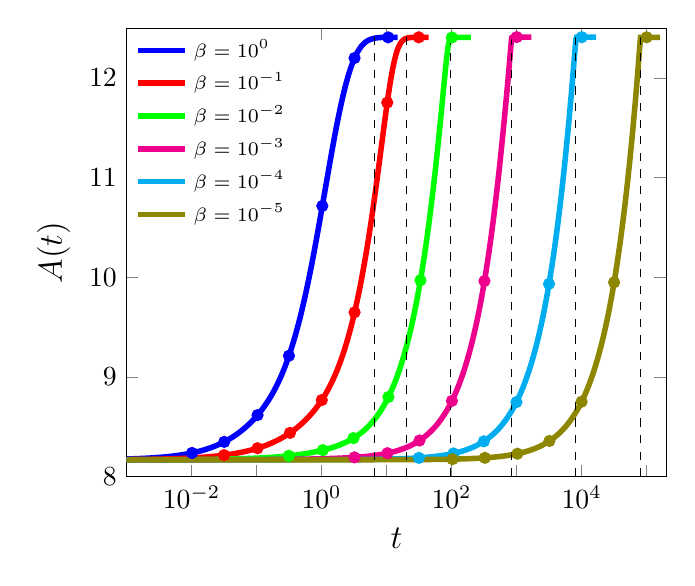
\begin{tikzpicture}[scale=1]

  \begin{axis}[
    xmin = 1e-3,
    xmax = 200000,
    xmode = log,
    xminorticks = false,
    xtick = {1e-3,1e-2,1e-1,1e0,1e1,1e2,1e3,1e4,1e5},
    xticklabels = {,$10^{-2}$,,$10^0$,,$10^2$,,$10^4$},
    ymin = 8,
    ymax = 12.5,
    xlabel = {\large $t$},
    ylabel = {\large ${A}(t)$},
    ylabel near ticks,
    legend entries = {$\beta=10^{0}$,
    $\beta = 10^{-1}$,
    $\beta = 10^{-2}$,
    $\beta = 10^{-3}$,
    $\beta = 10^{-4}$,
    $\beta = 10^{-5}$},
    legend cell align=left,
    legend style={draw=none,font=\scriptsize},
    legend style={at={(0.0,1.00)},anchor=north west}
  ]

\addplot[blue, line width=2pt] coordinates{
(9.4768e-04,8.1757e+00)
(9.8663e-04,8.1760e+00)
(1.0241e-03,8.1763e+00)
(1.0646e-03,8.1766e+00)
(1.1067e-03,8.1769e+00)
(1.1499e-03,8.1772e+00)
(1.1950e-03,8.1776e+00)
(1.2408e-03,8.1779e+00)
(1.2898e-03,8.1783e+00)
(1.3376e-03,8.1787e+00)
(1.3891e-03,8.1791e+00)
(1.4415e-03,8.1795e+00)
(1.4973e-03,8.1799e+00)
(1.5520e-03,8.1803e+00)
(1.6111e-03,8.1807e+00)
(1.6704e-03,8.1812e+00)
(1.7345e-03,8.1817e+00)
(1.7963e-03,8.1821e+00)
(1.8631e-03,8.1826e+00)
(1.9319e-03,8.1831e+00)
(2.0033e-03,8.1837e+00)
(2.0766e-03,8.1842e+00)
(2.1534e-03,8.1848e+00)
(2.2309e-03,8.1853e+00)
(2.3143e-03,8.1859e+00)
(2.3948e-03,8.1865e+00)
(2.4817e-03,8.1872e+00)
(2.5712e-03,8.1878e+00)
(2.6643e-03,8.1885e+00)
(2.7595e-03,8.1892e+00)
(2.8596e-03,8.1899e+00)
(2.9601e-03,8.1906e+00)
(3.0687e-03,8.1914e+00)
(3.1734e-03,8.1921e+00)
(3.2864e-03,8.1929e+00)
(3.4030e-03,8.1937e+00)
(3.5239e-03,8.1945e+00)
(3.6482e-03,8.1954e+00)
(3.7780e-03,8.1963e+00)
(3.9097e-03,8.1972e+00)
(4.0504e-03,8.1982e+00)
(4.1879e-03,8.1991e+00)
(4.3365e-03,8.2001e+00)
(4.4863e-03,8.2011e+00)
(4.6479e-03,8.2022e+00)
(4.8033e-03,8.2033e+00)
(4.9712e-03,8.2044e+00)
(5.1453e-03,8.2055e+00)
(5.3244e-03,8.2067e+00)
(5.5112e-03,8.2079e+00)
(5.7014e-03,8.2092e+00)
(5.9033e-03,8.2105e+00)
(6.1030e-03,8.2118e+00)
(6.3188e-03,8.2132e+00)
(6.5324e-03,8.2145e+00)
(6.7631e-03,8.2160e+00)
(6.9913e-03,8.2174e+00)
(7.2378e-03,8.2190e+00)
(7.4822e-03,8.2205e+00)
(7.7461e-03,8.2222e+00)
(8.0072e-03,8.2238e+00)
(8.2892e-03,8.2255e+00)
(8.5694e-03,8.2272e+00)
(8.8720e-03,8.2291e+00)
(9.1711e-03,8.2309e+00)
(9.4941e-03,8.2328e+00)
(9.8167e-03,8.2347e+00)
(1.0165e-02,8.2368e+00)
(1.0508e-02,8.2388e+00)
(1.0878e-02,8.2410e+00)
(1.1251e-02,8.2431e+00)
(1.1655e-02,8.2455e+00)
(1.2046e-02,8.2477e+00)
(1.2468e-02,8.2501e+00)
(1.2905e-02,8.2526e+00)
(1.3358e-02,8.2551e+00)
(1.3828e-02,8.2577e+00)
(1.4314e-02,8.2604e+00)
(1.4818e-02,8.2632e+00)
(1.5339e-02,8.2660e+00)
(1.5881e-02,8.2690e+00)
(1.6439e-02,8.2720e+00)
(1.7023e-02,8.2751e+00)
(1.7615e-02,8.2782e+00)
(1.8249e-02,8.2815e+00)
(1.8871e-02,8.2848e+00)
(1.9543e-02,8.2883e+00)
(2.0220e-02,8.2917e+00)
(2.0952e-02,8.2955e+00)
(2.1659e-02,8.2990e+00)
(2.2423e-02,8.3029e+00)
(2.3213e-02,8.3068e+00)
(2.4034e-02,8.3109e+00)
(2.4880e-02,8.3150e+00)
(2.5764e-02,8.3193e+00)
(2.6671e-02,8.3237e+00)
(2.7629e-02,8.3282e+00)
(2.8594e-02,8.3328e+00)
(2.9636e-02,8.3377e+00)
(3.0663e-02,8.3425e+00)
(3.1772e-02,8.3476e+00)
(3.2911e-02,8.3528e+00)
(3.4123e-02,8.3583e+00)
(3.5342e-02,8.3638e+00)
(3.6660e-02,8.3697e+00)
(3.7985e-02,8.3755e+00)
(3.9416e-02,8.3818e+00)
(4.0867e-02,8.3880e+00)
(4.2434e-02,8.3947e+00)
(4.4013e-02,8.4014e+00)
(4.5717e-02,8.4085e+00)
(4.7458e-02,8.4157e+00)
(4.9338e-02,8.4234e+00)
(5.1222e-02,8.4311e+00)
(5.3258e-02,8.4392e+00)
(5.5352e-02,8.4475e+00)
(5.7597e-02,8.4562e+00)
(5.9853e-02,8.4649e+00)
(6.2290e-02,8.4741e+00)
(6.4760e-02,8.4834e+00)
(6.7428e-02,8.4933e+00)
(7.0077e-02,8.5029e+00)
(7.2937e-02,8.5133e+00)
(7.5840e-02,8.5236e+00)
(7.8966e-02,8.5346e+00)
(8.2030e-02,8.5452e+00)
(8.5339e-02,8.5565e+00)
(8.8709e-02,8.5680e+00)
(9.2296e-02,8.5799e+00)
(9.5855e-02,8.5917e+00)
(9.9698e-02,8.6043e+00)
(1.0351e-01,8.6166e+00)
(1.0763e-01,8.6298e+00)
(1.1171e-01,8.6427e+00)
(1.1612e-01,8.6565e+00)
(1.2050e-01,8.6701e+00)
(1.2523e-01,8.6846e+00)
(1.2994e-01,8.6990e+00)
(1.3502e-01,8.7143e+00)
(1.4009e-01,8.7295e+00)
(1.4556e-01,8.7458e+00)
(1.5104e-01,8.7619e+00)
(1.5695e-01,8.7792e+00)
(1.6288e-01,8.7965e+00)
(1.6930e-01,8.8150e+00)
(1.7576e-01,8.8335e+00)
(1.8273e-01,8.8533e+00)
(1.8981e-01,8.8734e+00)
(1.9746e-01,8.8949e+00)
(2.0523e-01,8.9166e+00)
(2.1362e-01,8.9400e+00)
(2.2228e-01,8.9639e+00)
(2.3165e-01,8.9896e+00)
(2.4123e-01,9.0158e+00)
(2.5159e-01,9.0440e+00)
(2.6259e-01,9.0737e+00)
(2.7431e-01,9.1051e+00)
(2.8683e-01,9.1385e+00)
(3.0026e-01,9.1741e+00)
(3.1471e-01,9.2121e+00)
(3.3031e-01,9.2528e+00)
(3.4716e-01,9.2965e+00)
(3.6536e-01,9.3432e+00)
(3.8502e-01,9.3931e+00)
(4.0625e-01,9.4465e+00)
(4.2917e-01,9.5035e+00)
(4.5393e-01,9.5642e+00)
(4.8067e-01,9.6288e+00)
(5.0955e-01,9.6975e+00)
(5.4074e-01,9.7703e+00)
(5.7443e-01,9.8473e+00)
(6.1081e-01,9.9285e+00)
(6.5010e-01,1.0014e+01)
(6.9253e-01,1.0104e+01)
(7.3784e-01,1.0196e+01)
(7.8261e-01,1.0285e+01)
(8.3076e-01,1.0377e+01)
(8.7692e-01,1.0462e+01)
(9.2677e-01,1.0550e+01)
(9.7489e-01,1.0631e+01)
(1.0269e+00,1.0716e+01)
(1.0764e+00,1.0793e+01)
(1.1300e+00,1.0872e+01)
(1.1822e+00,1.0946e+01)
(1.2385e+00,1.1022e+01)
(1.2927e+00,1.1092e+01)
(1.3512e+00,1.1163e+01)
(1.4092e+00,1.1230e+01)
(1.4714e+00,1.1298e+01)
(1.5325e+00,1.1361e+01)
(1.5985e+00,1.1426e+01)
(1.6641e+00,1.1485e+01)
(1.7349e+00,1.1546e+01)
(1.8052e+00,1.1602e+01)
(1.8810e+00,1.1659e+01)
(1.9574e+00,1.1712e+01)
(2.0400e+00,1.1765e+01)
(2.1224e+00,1.1814e+01)
(2.2113e+00,1.1863e+01)
(2.3022e+00,1.1909e+01)
(2.4001e+00,1.1954e+01)
(2.4986e+00,1.1995e+01)
(2.6050e+00,1.2035e+01)
(2.7145e+00,1.2072e+01)
(2.8326e+00,1.2108e+01)
(2.9520e+00,1.2141e+01)
(3.0811e+00,1.2172e+01)
(3.2159e+00,1.2201e+01)
(3.3602e+00,1.2228e+01)
(3.5098e+00,1.2252e+01)
(3.6714e+00,1.2274e+01)
(3.8404e+00,1.2294e+01)
(4.0230e+00,1.2313e+01)
(4.2172e+00,1.2329e+01)
(4.4270e+00,1.2343e+01)
(4.6535e+00,1.2356e+01)
(4.8981e+00,1.2367e+01)
(5.1624e+00,1.2376e+01)
(5.4477e+00,1.2384e+01)
(5.7559e+00,1.2390e+01)
(6.0887e+00,1.2395e+01)
(6.4482e+00,1.2399e+01)
(6.8364e+00,1.2402e+01)
(7.2557e+00,1.2404e+01)
(7.7086e+00,1.2406e+01)
(8.1976e+00,1.2407e+01)
(8.7258e+00,1.2408e+01)
(9.2962e+00,1.2408e+01)
(9.9123e+00,1.2408e+01)
(1.0578e+01,1.2408e+01)
(1.1296e+01,1.2409e+01)
(1.2072e+01,1.2409e+01)
(1.2910e+01,1.2409e+01)
(1.3816e+01,1.2409e+01)
(1.4793e+01,1.2409e+01)
};

\addplot[red, line width=2pt] coordinates{
(8.9801e-04,8.1703e+00)
(9.6711e-04,8.1704e+00)
(1.0378e-03,8.1706e+00)
(1.1141e-03,8.1707e+00)
(1.1924e-03,8.1709e+00)
(1.2769e-03,8.1711e+00)
(1.3627e-03,8.1713e+00)
(1.4554e-03,8.1715e+00)
(1.5509e-03,8.1717e+00)
(1.6540e-03,8.1719e+00)
(1.7574e-03,8.1721e+00)
(1.8690e-03,8.1723e+00)
(1.9858e-03,8.1726e+00)
(2.1089e-03,8.1728e+00)
(2.2403e-03,8.1731e+00)
(2.3705e-03,8.1733e+00)
(2.5112e-03,8.1736e+00)
(2.6632e-03,8.1739e+00)
(2.8177e-03,8.1742e+00)
(2.9847e-03,8.1745e+00)
(3.1555e-03,8.1748e+00)
(3.3400e-03,8.1752e+00)
(3.5266e-03,8.1755e+00)
(3.7281e-03,8.1759e+00)
(3.9356e-03,8.1763e+00)
(4.1597e-03,8.1767e+00)
(4.3833e-03,8.1771e+00)
(4.6247e-03,8.1775e+00)
(4.8783e-03,8.1780e+00)
(5.1431e-03,8.1784e+00)
(5.4224e-03,8.1789e+00)
(5.7119e-03,8.1794e+00)
(6.0208e-03,8.1799e+00)
(6.3343e-03,8.1805e+00)
(6.6730e-03,8.1810e+00)
(7.0173e-03,8.1816e+00)
(7.3892e-03,8.1822e+00)
(7.7661e-03,8.1828e+00)
(8.1731e-03,8.1835e+00)
(8.5876e-03,8.1841e+00)
(9.0353e-03,8.1848e+00)
(9.4873e-03,8.1855e+00)
(9.9753e-03,8.1863e+00)
(1.0475e-02,8.1870e+00)
(1.1015e-02,8.1878e+00)
(1.1555e-02,8.1886e+00)
(1.2138e-02,8.1895e+00)
(1.2744e-02,8.1904e+00)
(1.3386e-02,8.1913e+00)
(1.4046e-02,8.1922e+00)
(1.4759e-02,8.1933e+00)
(1.5466e-02,8.1942e+00)
(1.6231e-02,8.1953e+00)
(1.7035e-02,8.1964e+00)
(1.7871e-02,8.1975e+00)
(1.8756e-02,8.1987e+00)
(1.9666e-02,8.1999e+00)
(2.0647e-02,8.2012e+00)
(2.1626e-02,8.2024e+00)
(2.2683e-02,8.2038e+00)
(2.3789e-02,8.2052e+00)
(2.4950e-02,8.2066e+00)
(2.6162e-02,8.2081e+00)
(2.7438e-02,8.2097e+00)
(2.8763e-02,8.2113e+00)
(3.0173e-02,8.2129e+00)
(3.1613e-02,8.2146e+00)
(3.3168e-02,8.2164e+00)
(3.4735e-02,8.2182e+00)
(3.6426e-02,8.2201e+00)
(3.8172e-02,8.2221e+00)
(4.0050e-02,8.2242e+00)
(4.1932e-02,8.2262e+00)
(4.3965e-02,8.2284e+00)
(4.6084e-02,8.2306e+00)
(4.8327e-02,8.2330e+00)
(5.0644e-02,8.2354e+00)
(5.3137e-02,8.2380e+00)
(5.5643e-02,8.2405e+00)
(5.8350e-02,8.2432e+00)
(6.1172e-02,8.2460e+00)
(6.4169e-02,8.2489e+00)
(6.7256e-02,8.2518e+00)
(7.0590e-02,8.2550e+00)
(7.3941e-02,8.2581e+00)
(7.7560e-02,8.2615e+00)
(8.1344e-02,8.2649e+00)
(8.5342e-02,8.2685e+00)
(8.9492e-02,8.2722e+00)
(9.3930e-02,8.2760e+00)
(9.8442e-02,8.2799e+00)
(1.0331e-01,8.2841e+00)
(1.0830e-01,8.2882e+00)
(1.1368e-01,8.2927e+00)
(1.1914e-01,8.2971e+00)
(1.2504e-01,8.3019e+00)
(1.3111e-01,8.3067e+00)
(1.3768e-01,8.3118e+00)
(1.4432e-01,8.3169e+00)
(1.5150e-01,8.3224e+00)
(1.5905e-01,8.3280e+00)
(1.6705e-01,8.3339e+00)
(1.7546e-01,8.3400e+00)
(1.8446e-01,8.3465e+00)
(1.9382e-01,8.3531e+00)
(2.0392e-01,8.3601e+00)
(2.1449e-01,8.3673e+00)
(2.2590e-01,8.3750e+00)
(2.3780e-01,8.3829e+00)
(2.5065e-01,8.3912e+00)
(2.6410e-01,8.3999e+00)
(2.7863e-01,8.4090e+00)
(2.9359e-01,8.4183e+00)
(3.0974e-01,8.4281e+00)
(3.2647e-01,8.4381e+00)
(3.4453e-01,8.4487e+00)
(3.6267e-01,8.4592e+00)
(3.8226e-01,8.4703e+00)
(4.0247e-01,8.4815e+00)
(4.2405e-01,8.4934e+00)
(4.4580e-01,8.5051e+00)
(4.6929e-01,8.5175e+00)
(4.9301e-01,8.5299e+00)
(5.1862e-01,8.5430e+00)
(5.4454e-01,8.5560e+00)
(5.7254e-01,8.5699e+00)
(6.0108e-01,8.5839e+00)
(6.3190e-01,8.5988e+00)
(6.6353e-01,8.6138e+00)
(6.9769e-01,8.6298e+00)
(7.3322e-01,8.6462e+00)
(7.7158e-01,8.6638e+00)
(8.1191e-01,8.6820e+00)
(8.5546e-01,8.7014e+00)
(9.0232e-01,8.7221e+00)
(9.5293e-01,8.7442e+00)
(1.0076e+00,8.7678e+00)
(1.0666e+00,8.7930e+00)
(1.1304e+00,8.8201e+00)
(1.1992e+00,8.8491e+00)
(1.2736e+00,8.8801e+00)
(1.3539e+00,8.9134e+00)
(1.4406e+00,8.9491e+00)
(1.5343e+00,8.9874e+00)
(1.6355e+00,9.0285e+00)
(1.7447e+00,9.0726e+00)
(1.8627e+00,9.1201e+00)
(1.9901e+00,9.1710e+00)
(2.1278e+00,9.2257e+00)
(2.2764e+00,9.2844e+00)
(2.4370e+00,9.3474e+00)
(2.6103e+00,9.4150e+00)
(2.7976e+00,9.4875e+00)
(2.9998e+00,9.5652e+00)
(3.2182e+00,9.6483e+00)
(3.4541e+00,9.7372e+00)
(3.7088e+00,9.8322e+00)
(3.9840e+00,9.9336e+00)
(4.2811e+00,1.0041e+01)
(4.6020e+00,1.0156e+01)
(4.9486e+00,1.0278e+01)
(5.3229e+00,1.0406e+01)
(5.6770e+00,1.0525e+01)
(5.9957e+00,1.0630e+01)
(6.3399e+00,1.0740e+01)
(6.7116e+00,1.0856e+01)
(7.0771e+00,1.0967e+01)
(7.4393e+00,1.1072e+01)
(7.7963e+00,1.1173e+01)
(8.1517e+00,1.1270e+01)
(8.5014e+00,1.1361e+01)
(8.8524e+00,1.1449e+01)
(9.1955e+00,1.1530e+01)
(9.5460e+00,1.1610e+01)
(9.8822e+00,1.1682e+01)
(1.0239e+01,1.1754e+01)
(1.0565e+01,1.1816e+01)
(1.0917e+01,1.1878e+01)
(1.1259e+01,1.1935e+01)
(1.1625e+01,1.1990e+01)
(1.1965e+01,1.2037e+01)
(1.2333e+01,1.2084e+01)
(1.2707e+01,1.2126e+01)
(1.3095e+01,1.2166e+01)
(1.3492e+01,1.2201e+01)
(1.3914e+01,1.2234e+01)
(1.4341e+01,1.2263e+01)
(1.4803e+01,1.2289e+01)
(1.5291e+01,1.2312e+01)
(1.5819e+01,1.2332e+01)
(1.6387e+01,1.2350e+01)
(1.7001e+01,1.2364e+01)
(1.7664e+01,1.2376e+01)
(1.8381e+01,1.2385e+01)
(1.9154e+01,1.2393e+01)
(1.9989e+01,1.2398e+01)
(2.0891e+01,1.2402e+01)
(2.1866e+01,1.2404e+01)
(2.2918e+01,1.2406e+01)
(2.4054e+01,1.2407e+01)
(2.5281e+01,1.2408e+01)
(2.6607e+01,1.2408e+01)
(2.8038e+01,1.2409e+01)
(2.9584e+01,1.2409e+01)
(3.1254e+01,1.2409e+01)
(3.3057e+01,1.2409e+01)
(3.5005e+01,1.2409e+01)
(3.7108e+01,1.2409e+01)
(3.9380e+01,1.2409e+01)
(4.1833e+01,1.2409e+01)
(4.4483e+01,1.2409e+01)
};

\addplot[green, line width=2pt] coordinates{
(8.4580e-04,8.1684e+00)
(9.4755e-04,8.1684e+00)
(1.0574e-03,8.1684e+00)
(1.1761e-03,8.1685e+00)
(1.3043e-03,8.1685e+00)
(1.4427e-03,8.1685e+00)
(1.5922e-03,8.1686e+00)
(1.7537e-03,8.1686e+00)
(1.9281e-03,8.1687e+00)
(2.1164e-03,8.1687e+00)
(2.3198e-03,8.1688e+00)
(2.5395e-03,8.1688e+00)
(2.7768e-03,8.1689e+00)
(3.0330e-03,8.1690e+00)
(3.3097e-03,8.1690e+00)
(3.6086e-03,8.1691e+00)
(3.9314e-03,8.1692e+00)
(4.2800e-03,8.1693e+00)
(4.6564e-03,8.1694e+00)
(5.0631e-03,8.1695e+00)
(5.5022e-03,8.1696e+00)
(5.9737e-03,8.1697e+00)
(6.4672e-03,8.1698e+00)
(7.0003e-03,8.1699e+00)
(7.5566e-03,8.1700e+00)
(8.1573e-03,8.1702e+00)
(8.7843e-03,8.1703e+00)
(9.4615e-03,8.1704e+00)
(1.0165e-02,8.1706e+00)
(1.0925e-02,8.1707e+00)
(1.1717e-02,8.1709e+00)
(1.2573e-02,8.1711e+00)
(1.3457e-02,8.1713e+00)
(1.4411e-02,8.1715e+00)
(1.5409e-02,8.1717e+00)
(1.6487e-02,8.1719e+00)
(1.7591e-02,8.1721e+00)
(1.8782e-02,8.1723e+00)
(2.0041e-02,8.1725e+00)
(2.1375e-02,8.1728e+00)
(2.2780e-02,8.1730e+00)
(2.4277e-02,8.1733e+00)
(2.5838e-02,8.1736e+00)
(2.7524e-02,8.1739e+00)
(2.9244e-02,8.1742e+00)
(3.1103e-02,8.1745e+00)
(3.3064e-02,8.1748e+00)
(3.5141e-02,8.1752e+00)
(3.7327e-02,8.1755e+00)
(3.9651e-02,8.1759e+00)
(4.2083e-02,8.1763e+00)
(4.4693e-02,8.1767e+00)
(4.7379e-02,8.1771e+00)
(5.0279e-02,8.1776e+00)
(5.3296e-02,8.1781e+00)
(5.6554e-02,8.1785e+00)
(5.9884e-02,8.1790e+00)
(6.3482e-02,8.1796e+00)
(6.7262e-02,8.1801e+00)
(7.1292e-02,8.1807e+00)
(7.5489e-02,8.1813e+00)
(8.0022e-02,8.1819e+00)
(8.4654e-02,8.1825e+00)
(8.9657e-02,8.1832e+00)
(9.4927e-02,8.1839e+00)
(1.0053e-01,8.1846e+00)
(1.0640e-01,8.1853e+00)
(1.1270e-01,8.1861e+00)
(1.1920e-01,8.1869e+00)
(1.2623e-01,8.1878e+00)
(1.3354e-01,8.1887e+00)
(1.4144e-01,8.1896e+00)
(1.4957e-01,8.1906e+00)
(1.5834e-01,8.1916e+00)
(1.6755e-01,8.1926e+00)
(1.7743e-01,8.1938e+00)
(1.8767e-01,8.1949e+00)
(1.9873e-01,8.1961e+00)
(2.1022e-01,8.1973e+00)
(2.2263e-01,8.1986e+00)
(2.3551e-01,8.2000e+00)
(2.4941e-01,8.2014e+00)
(2.6393e-01,8.2028e+00)
(2.7962e-01,8.2044e+00)
(2.9597e-01,8.2060e+00)
(3.1362e-01,8.2077e+00)
(3.3229e-01,8.2094e+00)
(3.5244e-01,8.2113e+00)
(3.7360e-01,8.2133e+00)
(3.9644e-01,8.2153e+00)
(4.2098e-01,8.2175e+00)
(4.4715e-01,8.2198e+00)
(4.7538e-01,8.2222e+00)
(5.0531e-01,8.2247e+00)
(5.3763e-01,8.2273e+00)
(5.7179e-01,8.2301e+00)
(6.0869e-01,8.2330e+00)
(6.4706e-01,8.2360e+00)
(6.8851e-01,8.2392e+00)
(7.3155e-01,8.2424e+00)
(7.7803e-01,8.2459e+00)
(8.2549e-01,8.2493e+00)
(8.7674e-01,8.2530e+00)
(9.3002e-01,8.2567e+00)
(9.8749e-01,8.2606e+00)
(1.0462e+00,8.2646e+00)
(1.1096e+00,8.2688e+00)
(1.1771e+00,8.2732e+00)
(1.2488e+00,8.2779e+00)
(1.3262e+00,8.2828e+00)
(1.4086e+00,8.2879e+00)
(1.4976e+00,8.2934e+00)
(1.5937e+00,8.2992e+00)
(1.6976e+00,8.3055e+00)
(1.8097e+00,8.3121e+00)
(1.9308e+00,8.3192e+00)
(2.0616e+00,8.3268e+00)
(2.2028e+00,8.3350e+00)
(2.3554e+00,8.3437e+00)
(2.5202e+00,8.3530e+00)
(2.6981e+00,8.3630e+00)
(2.8903e+00,8.3738e+00)
(3.0978e+00,8.3854e+00)
(3.3220e+00,8.3979e+00)
(3.5641e+00,8.4113e+00)
(3.8255e+00,8.4257e+00)
(4.1079e+00,8.4413e+00)
(4.4129e+00,8.4581e+00)
(4.7422e+00,8.4762e+00)
(5.0979e+00,8.4957e+00)
(5.4821e+00,8.5168e+00)
(5.8970e+00,8.5395e+00)
(6.3451e+00,8.5639e+00)
(6.8290e+00,8.5903e+00)
(7.3517e+00,8.6188e+00)
(7.9161e+00,8.6495e+00)
(8.5258e+00,8.6826e+00)
(9.1842e+00,8.7183e+00)
(9.8952e+00,8.7567e+00)
(1.0663e+01,8.7981e+00)
(1.1493e+01,8.8428e+00)
(1.2388e+01,8.8908e+00)
(1.3356e+01,8.9426e+00)
(1.4400e+01,8.9984e+00)
(1.5529e+01,9.0584e+00)
(1.6747e+01,9.1230e+00)
(1.8064e+01,9.1924e+00)
(1.9485e+01,9.2671e+00)
(2.1020e+01,9.3475e+00)
(2.2678e+01,9.4338e+00)
(2.4469e+01,9.5265e+00)
(2.6402e+01,9.6260e+00)
(2.8491e+01,9.7328e+00)
(3.0747e+01,9.8473e+00)
(3.3183e+01,9.9701e+00)
(3.5814e+01,1.0101e+01)
(3.8655e+01,1.0242e+01)
(4.1724e+01,1.0392e+01)
(4.5038e+01,1.0552e+01)
(4.8617e+01,1.0723e+01)
(5.2483e+01,1.0904e+01)
(5.6658e+01,1.1096e+01)
(5.9881e+01,1.1242e+01)
(6.2782e+01,1.1371e+01)
(6.5915e+01,1.1507e+01)
(6.8271e+01,1.1608e+01)
(7.0392e+01,1.1697e+01)
(7.2683e+01,1.1791e+01)
(7.4546e+01,1.1866e+01)
(7.6222e+01,1.1931e+01)
(7.8032e+01,1.1999e+01)
(7.9448e+01,1.2051e+01)
(8.0722e+01,1.2095e+01)
(8.2097e+01,1.2142e+01)
(8.3366e+01,1.2182e+01)
(8.4508e+01,1.2216e+01)
(8.5741e+01,1.2251e+01)
(8.6817e+01,1.2279e+01)
(8.7785e+01,1.2301e+01)
(8.8830e+01,1.2323e+01)
(8.9960e+01,1.2343e+01)
(9.1041e+01,1.2360e+01)
(9.2209e+01,1.2374e+01)
(9.3410e+01,1.2385e+01)
(9.4707e+01,1.2393e+01)
(9.6108e+01,1.2399e+01)
(9.7620e+01,1.2403e+01)
(9.9254e+01,1.2406e+01)
(1.0102e+02,1.2407e+01)
(1.0292e+02,1.2408e+01)
(1.0498e+02,1.2409e+01)
(1.0720e+02,1.2409e+01)
(1.0960e+02,1.2409e+01)
(1.1220e+02,1.2409e+01)
(1.1500e+02,1.2409e+01)
(1.1802e+02,1.2409e+01)
(1.2129e+02,1.2409e+01)
(1.2481e+02,1.2409e+01)
(1.2862e+02,1.2409e+01)
(1.3274e+02,1.2409e+01)
(1.3718e+02,1.2409e+01)
(1.4198e+02,1.2409e+01)
(1.4716e+02,1.2409e+01)
(1.5276e+02,1.2409e+01)
(1.5880e+02,1.2409e+01)
(1.6533e+02,1.2409e+01)
(1.7238e+02,1.2409e+01)
(1.8000e+02,1.2409e+01)
(1.8822e+02,1.2409e+01)
(1.9710e+02,1.2409e+01)
};

\addplot[magenta, line width=2pt] coordinates{
(7.8511e-04,8.1682e+00)
(9.0052e-04,8.1682e+00)
(1.0252e-03,8.1682e+00)
(1.1598e-03,8.1682e+00)
(1.3052e-03,8.1682e+00)
(1.4622e-03,8.1682e+00)
(1.6318e-03,8.1682e+00)
(1.8149e-03,8.1682e+00)
(2.0127e-03,8.1682e+00)
(2.2263e-03,8.1682e+00)
(2.4570e-03,8.1682e+00)
(2.7062e-03,8.1682e+00)
(2.9753e-03,8.1682e+00)
(3.2659e-03,8.1682e+00)
(3.5798e-03,8.1682e+00)
(3.9188e-03,8.1682e+00)
(4.2849e-03,8.1683e+00)
(4.6803e-03,8.1683e+00)
(5.1073e-03,8.1683e+00)
(5.5685e-03,8.1683e+00)
(6.0666e-03,8.1683e+00)
(6.6045e-03,8.1683e+00)
(7.1855e-03,8.1683e+00)
(7.8129e-03,8.1683e+00)
(8.4905e-03,8.1684e+00)
(9.2224e-03,8.1684e+00)
(9.9991e-03,8.1684e+00)
(1.0827e-02,8.1684e+00)
(1.1702e-02,8.1684e+00)
(1.2641e-02,8.1684e+00)
(1.3621e-02,8.1685e+00)
(1.4679e-02,8.1685e+00)
(1.5779e-02,8.1685e+00)
(1.6968e-02,8.1685e+00)
(1.8208e-02,8.1686e+00)
(1.9547e-02,8.1686e+00)
(2.0933e-02,8.1686e+00)
(2.2430e-02,8.1686e+00)
(2.3996e-02,8.1687e+00)
(2.5687e-02,8.1687e+00)
(2.7422e-02,8.1687e+00)
(2.9295e-02,8.1688e+00)
(3.1276e-02,8.1688e+00)
(3.3376e-02,8.1689e+00)
(3.5593e-02,8.1689e+00)
(3.7949e-02,8.1689e+00)
(4.0425e-02,8.1690e+00)
(4.3074e-02,8.1690e+00)
(4.5826e-02,8.1691e+00)
(4.8797e-02,8.1691e+00)
(5.1865e-02,8.1692e+00)
(5.5178e-02,8.1692e+00)
(5.8630e-02,8.1693e+00)
(6.2358e-02,8.1693e+00)
(6.6187e-02,8.1694e+00)
(7.0322e-02,8.1695e+00)
(7.4666e-02,8.1695e+00)
(7.9318e-02,8.1696e+00)
(8.4141e-02,8.1697e+00)
(8.9350e-02,8.1697e+00)
(9.4748e-02,8.1698e+00)
(1.0058e-01,8.1699e+00)
(1.0663e-01,8.1700e+00)
(1.1316e-01,8.1701e+00)
(1.1994e-01,8.1702e+00)
(1.2725e-01,8.1703e+00)
(1.3486e-01,8.1703e+00)
(1.4308e-01,8.1705e+00)
(1.5159e-01,8.1706e+00)
(1.6079e-01,8.1707e+00)
(1.7039e-01,8.1708e+00)
(1.8076e-01,8.1709e+00)
(1.9148e-01,8.1710e+00)
(2.0304e-01,8.1712e+00)
(2.1521e-01,8.1713e+00)
(2.2829e-01,8.1715e+00)
(2.4187e-01,8.1716e+00)
(2.5654e-01,8.1718e+00)
(2.7191e-01,8.1719e+00)
(2.8850e-01,8.1721e+00)
(3.0579e-01,8.1723e+00)
(3.2446e-01,8.1725e+00)
(3.4425e-01,8.1727e+00)
(3.6555e-01,8.1729e+00)
(3.8802e-01,8.1731e+00)
(4.1229e-01,8.1734e+00)
(4.3823e-01,8.1736e+00)
(4.6618e-01,8.1739e+00)
(4.9600e-01,8.1741e+00)
(5.2821e-01,8.1744e+00)
(5.6259e-01,8.1747e+00)
(5.9972e-01,8.1751e+00)
(6.3901e-01,8.1754e+00)
(6.8145e-01,8.1758e+00)
(7.2600e-01,8.1761e+00)
(7.7412e-01,8.1765e+00)
(8.2397e-01,8.1769e+00)
(8.7782e-01,8.1773e+00)
(9.3363e-01,8.1778e+00)
(9.9391e-01,8.1782e+00)
(1.0560e+00,8.1787e+00)
(1.1231e+00,8.1792e+00)
(1.1935e+00,8.1797e+00)
(1.2696e+00,8.1802e+00)
(1.3493e+00,8.1807e+00)
(1.4353e+00,8.1813e+00)
(1.5282e+00,8.1819e+00)
(1.6286e+00,8.1826e+00)
(1.7370e+00,8.1833e+00)
(1.8540e+00,8.1841e+00)
(1.9805e+00,8.1849e+00)
(2.1170e+00,8.1857e+00)
(2.2645e+00,8.1866e+00)
(2.4237e+00,8.1876e+00)
(2.5957e+00,8.1887e+00)
(2.7815e+00,8.1898e+00)
(2.9821e+00,8.1910e+00)
(3.1988e+00,8.1923e+00)
(3.4328e+00,8.1937e+00)
(3.6855e+00,8.1952e+00)
(3.9584e+00,8.1968e+00)
(4.2532e+00,8.1986e+00)
(4.5716e+00,8.2004e+00)
(4.9154e+00,8.2025e+00)
(5.2868e+00,8.2046e+00)
(5.6878e+00,8.2070e+00)
(6.1209e+00,8.2096e+00)
(6.5887e+00,8.2123e+00)
(7.0939e+00,8.2153e+00)
(7.6395e+00,8.2185e+00)
(8.2288e+00,8.2219e+00)
(8.8652e+00,8.2257e+00)
(9.5525e+00,8.2297e+00)
(1.0295e+01,8.2341e+00)
(1.1096e+01,8.2388e+00)
(1.1962e+01,8.2439e+00)
(1.2897e+01,8.2494e+00)
(1.3907e+01,8.2553e+00)
(1.4998e+01,8.2617e+00)
(1.6176e+01,8.2686e+00)
(1.7448e+01,8.2760e+00)
(1.8822e+01,8.2841e+00)
(2.0306e+01,8.2928e+00)
(2.1908e+01,8.3021e+00)
(2.3639e+01,8.3123e+00)
(2.5509e+01,8.3232e+00)
(2.7527e+01,8.3350e+00)
(2.9708e+01,8.3477e+00)
(3.2062e+01,8.3614e+00)
(3.4605e+01,8.3763e+00)
(3.7352e+01,8.3922e+00)
(4.0318e+01,8.4095e+00)
(4.3522e+01,8.4281e+00)
(4.6982e+01,8.4482e+00)
(5.0718e+01,8.4698e+00)
(5.4754e+01,8.4932e+00)
(5.9112e+01,8.5184e+00)
(6.3819e+01,8.5455e+00)
(6.8903e+01,8.5748e+00)
(7.4393e+01,8.6064e+00)
(8.0323e+01,8.6404e+00)
(8.6727e+01,8.6771e+00)
(9.3643e+01,8.7167e+00)
(1.0111e+02,8.7592e+00)
(1.0918e+02,8.8051e+00)
(1.1789e+02,8.8545e+00)
(1.2730e+02,8.9077e+00)
(1.3746e+02,8.9650e+00)
(1.4844e+02,9.0266e+00)
(1.6029e+02,9.0930e+00)
(1.7309e+02,9.1643e+00)
(1.8692e+02,9.2410e+00)
(2.0185e+02,9.3234e+00)
(2.1798e+02,9.4120e+00)
(2.3539e+02,9.5071e+00)
(2.5420e+02,9.6093e+00)
(2.7452e+02,9.7189e+00)
(2.9646e+02,9.8364e+00)
(3.2015e+02,9.9624e+00)
(3.4574e+02,1.0097e+01)
(3.7338e+02,1.0242e+01)
(4.0323e+02,1.0396e+01)
(4.3546e+02,1.0561e+01)
(4.7028e+02,1.0737e+01)
(5.0788e+02,1.0924e+01)
(5.4849e+02,1.1122e+01)
(5.9234e+02,1.1332e+01)
(6.3971e+02,1.1553e+01)
(6.9087e+02,1.1783e+01)
(7.3860e+02,1.1988e+01)
(7.6471e+02,1.2103e+01)
(7.8821e+02,1.2203e+01)
(7.9978e+02,1.2253e+01)
(8.1019e+02,1.2297e+01)
(8.1786e+02,1.2328e+01)
(8.2476e+02,1.2355e+01)
(8.2894e+02,1.2370e+01)
(8.3270e+02,1.2383e+01)
(8.3676e+02,1.2394e+01)
(8.4008e+02,1.2402e+01)
(8.4307e+02,1.2406e+01)
(8.4630e+02,1.2409e+01)
(8.4979e+02,1.2410e+01)
(8.5355e+02,1.2410e+01)
(8.5762e+02,1.2411e+01)
(8.6201e+02,1.2411e+01)
(8.6676e+02,1.2411e+01)
(8.7188e+02,1.2411e+01)
(8.7741e+02,1.2411e+01)
(8.8339e+02,1.2411e+01)
(8.8984e+02,1.2411e+01)
(8.9681e+02,1.2411e+01)
(9.0434e+02,1.2411e+01)
(9.1247e+02,1.2411e+01)
(9.2125e+02,1.2411e+01)
(9.3074e+02,1.2411e+01)
(9.4098e+02,1.2411e+01)
(9.5204e+02,1.2411e+01)
(9.6399e+02,1.2411e+01)
(9.7689e+02,1.2411e+01)
(9.9082e+02,1.2411e+01)
(1.0059e+03,1.2411e+01)
(1.0221e+03,1.2411e+01)
(1.0397e+03,1.2411e+01)
(1.0586e+03,1.2411e+01)
(1.0791e+03,1.2411e+01)
(1.1012e+03,1.2411e+01)
(1.1251e+03,1.2411e+01)
(1.1509e+03,1.2411e+01)
(1.1787e+03,1.2411e+01)
(1.2088e+03,1.2411e+01)
(1.2413e+03,1.2411e+01)
(1.2764e+03,1.2411e+01)
(1.3143e+03,1.2411e+01)
(1.3552e+03,1.2411e+01)
(1.3994e+03,1.2411e+01)
(1.4472e+03,1.2411e+01)
(1.4987e+03,1.2411e+01)
(1.5544e+03,1.2411e+01)
(1.6145e+03,1.2411e+01)
(1.6795e+03,1.2411e+01)
};

\addplot[cyan, line width=2pt] coordinates{
(8.1786e-04,8.1681e+00)
(9.4671e-04,8.1681e+00)
(1.0859e-03,8.1681e+00)
(1.2362e-03,8.1681e+00)
(1.3985e-03,8.1681e+00)
(1.5738e-03,8.1681e+00)
(1.7632e-03,8.1681e+00)
(1.9676e-03,8.1681e+00)
(2.1885e-03,8.1681e+00)
(2.4270e-03,8.1681e+00)
(2.6846e-03,8.1681e+00)
(2.9628e-03,8.1681e+00)
(3.2632e-03,8.1681e+00)
(3.5877e-03,8.1682e+00)
(3.9381e-03,8.1682e+00)
(4.3166e-03,8.1682e+00)
(4.7254e-03,8.1682e+00)
(5.1669e-03,8.1682e+00)
(5.6436e-03,8.1682e+00)
(6.1586e-03,8.1682e+00)
(6.7147e-03,8.1682e+00)
(7.3153e-03,8.1682e+00)
(7.9639e-03,8.1682e+00)
(8.6645e-03,8.1682e+00)
(9.4210e-03,8.1682e+00)
(1.0214e-02,8.1682e+00)
(1.1071e-02,8.1682e+00)
(1.1964e-02,8.1682e+00)
(1.2929e-02,8.1682e+00)
(1.3939e-02,8.1682e+00)
(1.5030e-02,8.1682e+00)
(1.6161e-02,8.1682e+00)
(1.7381e-02,8.1682e+00)
(1.8664e-02,8.1682e+00)
(2.0045e-02,8.1682e+00)
(2.1470e-02,8.1682e+00)
(2.3010e-02,8.1682e+00)
(2.4627e-02,8.1682e+00)
(2.6364e-02,8.1682e+00)
(2.8162e-02,8.1682e+00)
(3.0104e-02,8.1682e+00)
(3.2128e-02,8.1682e+00)
(3.4315e-02,8.1682e+00)
(3.6564e-02,8.1682e+00)
(3.8994e-02,8.1682e+00)
(4.1545e-02,8.1682e+00)
(4.4281e-02,8.1682e+00)
(4.7112e-02,8.1682e+00)
(5.0169e-02,8.1682e+00)
(5.3346e-02,8.1682e+00)
(5.6777e-02,8.1683e+00)
(6.0318e-02,8.1683e+00)
(6.4142e-02,8.1683e+00)
(6.8131e-02,8.1683e+00)
(7.2439e-02,8.1683e+00)
(7.6859e-02,8.1683e+00)
(8.1633e-02,8.1683e+00)
(8.6663e-02,8.1683e+00)
(9.2024e-02,8.1683e+00)
(9.7633e-02,8.1683e+00)
(1.0369e-01,8.1683e+00)
(1.0989e-01,8.1683e+00)
(1.1660e-01,8.1683e+00)
(1.2368e-01,8.1683e+00)
(1.3121e-01,8.1684e+00)
(1.3915e-01,8.1684e+00)
(1.4762e-01,8.1684e+00)
(1.5649e-01,8.1684e+00)
(1.6606e-01,8.1684e+00)
(1.7592e-01,8.1684e+00)
(1.8656e-01,8.1684e+00)
(1.9782e-01,8.1684e+00)
(2.0981e-01,8.1685e+00)
(2.2242e-01,8.1685e+00)
(2.3598e-01,8.1685e+00)
(2.5007e-01,8.1685e+00)
(2.6529e-01,8.1685e+00)
(2.8125e-01,8.1685e+00)
(2.9849e-01,8.1685e+00)
(3.1645e-01,8.1686e+00)
(3.3585e-01,8.1686e+00)
(3.5648e-01,8.1686e+00)
(3.7861e-01,8.1686e+00)
(4.0213e-01,8.1687e+00)
(4.2752e-01,8.1687e+00)
(4.5449e-01,8.1687e+00)
(4.8362e-01,8.1687e+00)
(5.1489e-01,8.1688e+00)
(5.4849e-01,8.1688e+00)
(5.8452e-01,8.1688e+00)
(6.2316e-01,8.1688e+00)
(6.6440e-01,8.1689e+00)
(7.0851e-01,8.1689e+00)
(7.5520e-01,8.1690e+00)
(8.0510e-01,8.1690e+00)
(8.5737e-01,8.1690e+00)
(9.1358e-01,8.1691e+00)
(9.7150e-01,8.1691e+00)
(1.0341e+00,8.1692e+00)
(1.0993e+00,8.1692e+00)
(1.1697e+00,8.1693e+00)
(1.2428e+00,8.1693e+00)
(1.3218e+00,8.1694e+00)
(1.4067e+00,8.1694e+00)
(1.4977e+00,8.1695e+00)
(1.5960e+00,8.1696e+00)
(1.7022e+00,8.1696e+00)
(1.8169e+00,8.1697e+00)
(1.9407e+00,8.1698e+00)
(2.0744e+00,8.1699e+00)
(2.2189e+00,8.1699e+00)
(2.3749e+00,8.1700e+00)
(2.5434e+00,8.1701e+00)
(2.7253e+00,8.1703e+00)
(2.9218e+00,8.1704e+00)
(3.1341e+00,8.1705e+00)
(3.3633e+00,8.1706e+00)
(3.6108e+00,8.1708e+00)
(3.8782e+00,8.1710e+00)
(4.1669e+00,8.1711e+00)
(4.4787e+00,8.1713e+00)
(4.8155e+00,8.1715e+00)
(5.1793e+00,8.1717e+00)
(5.5721e+00,8.1720e+00)
(5.9963e+00,8.1722e+00)
(6.4545e+00,8.1725e+00)
(6.9494e+00,8.1728e+00)
(7.4838e+00,8.1731e+00)
(8.0610e+00,8.1734e+00)
(8.6844e+00,8.1738e+00)
(9.3576e+00,8.1742e+00)
(1.0085e+01,8.1746e+00)
(1.0870e+01,8.1751e+00)
(1.1718e+01,8.1756e+00)
(1.2634e+01,8.1761e+00)
(1.3623e+01,8.1767e+00)
(1.4692e+01,8.1774e+00)
(1.5845e+01,8.1781e+00)
(1.7091e+01,8.1788e+00)
(1.8437e+01,8.1796e+00)
(1.9891e+01,8.1804e+00)
(2.1460e+01,8.1814e+00)
(2.3156e+01,8.1824e+00)
(2.4987e+01,8.1835e+00)
(2.6964e+01,8.1846e+00)
(2.9100e+01,8.1859e+00)
(3.1406e+01,8.1873e+00)
(3.3897e+01,8.1887e+00)
(3.6587e+01,8.1903e+00)
(3.9493e+01,8.1921e+00)
(4.2631e+01,8.1939e+00)
(4.6020e+01,8.1959e+00)
(4.9680e+01,8.1981e+00)
(5.3633e+01,8.2004e+00)
(5.7902e+01,8.2030e+00)
(6.2513e+01,8.2057e+00)
(6.7492e+01,8.2086e+00)
(7.2870e+01,8.2118e+00)
(7.8678e+01,8.2153e+00)
(8.4951e+01,8.2190e+00)
(9.1725e+01,8.2230e+00)
(9.9042e+01,8.2273e+00)
(1.0694e+02,8.2320e+00)
(1.1548e+02,8.2370e+00)
(1.2469e+02,8.2424e+00)
(1.3465e+02,8.2483e+00)
(1.4540e+02,8.2547e+00)
(1.5701e+02,8.2615e+00)
(1.6955e+02,8.2689e+00)
(1.8309e+02,8.2769e+00)
(1.9772e+02,8.2855e+00)
(2.1351e+02,8.2948e+00)
(2.3057e+02,8.3048e+00)
(2.4900e+02,8.3157e+00)
(2.6889e+02,8.3274e+00)
(2.9038e+02,8.3400e+00)
(3.1359e+02,8.3536e+00)
(3.3866e+02,8.3683e+00)
(3.6573e+02,8.3842e+00)
(3.9497e+02,8.4013e+00)
(4.2654e+02,8.4197e+00)
(4.6064e+02,8.4396e+00)
(4.9747e+02,8.4611e+00)
(5.3725e+02,8.4842e+00)
(5.8021e+02,8.5092e+00)
(6.2660e+02,8.5361e+00)
(6.7671e+02,8.5651e+00)
(7.3083e+02,8.5963e+00)
(7.8927e+02,8.6300e+00)
(8.5239e+02,8.6663e+00)
(9.2056e+02,8.7054e+00)
(9.9418e+02,8.7475e+00)
(1.0737e+03,8.7928e+00)
(1.1596e+03,8.8415e+00)
(1.2523e+03,8.8940e+00)
(1.3523e+03,8.9503e+00)
(1.4523e+03,9.0064e+00)
(1.5523e+03,9.0623e+00)
(1.6523e+03,9.1181e+00)
(1.7523e+03,9.1736e+00)
(1.8523e+03,9.2290e+00)
(1.9523e+03,9.2843e+00)
(2.0523e+03,9.3393e+00)
(2.1523e+03,9.3942e+00)
(2.2523e+03,9.4489e+00)
(2.3523e+03,9.5035e+00)
(2.4523e+03,9.5579e+00)
(2.5523e+03,9.6121e+00)
(2.6523e+03,9.6662e+00)
(2.7523e+03,9.7201e+00)
(2.8523e+03,9.7738e+00)
(2.9523e+03,9.8274e+00)
(3.0523e+03,9.8808e+00)
(3.1523e+03,9.9341e+00)
(3.2523e+03,9.9872e+00)
(3.3523e+03,1.0040e+01)
(3.4523e+03,1.0093e+01)
(3.5523e+03,1.0146e+01)
(3.6523e+03,1.0198e+01)
(3.7523e+03,1.0250e+01)
(3.8523e+03,1.0303e+01)
(3.9523e+03,1.0355e+01)
(4.0523e+03,1.0407e+01)
(4.1523e+03,1.0458e+01)
(4.2523e+03,1.0510e+01)
(4.3523e+03,1.0561e+01)
(4.4523e+03,1.0613e+01)
(4.5523e+03,1.0664e+01)
(4.6523e+03,1.0715e+01)
(4.7523e+03,1.0766e+01)
(4.8523e+03,1.0817e+01)
(4.9523e+03,1.0867e+01)
(5.0523e+03,1.0918e+01)
(5.1523e+03,1.0968e+01)
(5.2523e+03,1.1018e+01)
(5.3523e+03,1.1068e+01)
(5.4523e+03,1.1118e+01)
(5.5523e+03,1.1167e+01)
(5.6523e+03,1.1217e+01)
(5.7523e+03,1.1266e+01)
(5.8523e+03,1.1316e+01)
(5.9523e+03,1.1365e+01)
(6.0523e+03,1.1414e+01)
(6.1523e+03,1.1463e+01)
(6.2523e+03,1.1511e+01)
(6.3523e+03,1.1560e+01)
(6.4523e+03,1.1608e+01)
(6.5523e+03,1.1656e+01)
(6.6523e+03,1.1704e+01)
(6.7523e+03,1.1752e+01)
(6.8523e+03,1.1799e+01)
(6.9523e+03,1.1847e+01)
(7.0523e+03,1.1894e+01)
(7.1523e+03,1.1940e+01)
(7.2523e+03,1.1987e+01)
(7.3523e+03,1.2033e+01)
(7.4523e+03,1.2079e+01)
(7.5523e+03,1.2125e+01)
(7.6523e+03,1.2170e+01)
(7.7523e+03,1.2214e+01)
(7.8523e+03,1.2257e+01)
(7.9523e+03,1.2300e+01)
(8.0523e+03,1.2340e+01)
(8.1523e+03,1.2376e+01)
(8.2523e+03,1.2402e+01)
(8.3523e+03,1.2410e+01)
(8.4523e+03,1.2410e+01)
(8.5523e+03,1.2410e+01)
(8.6523e+03,1.2410e+01)
(8.7523e+03,1.2410e+01)
(8.8523e+03,1.2410e+01)
(8.9523e+03,1.2410e+01)
(9.0523e+03,1.2410e+01)
(9.1523e+03,1.2410e+01)
(9.2523e+03,1.2410e+01)
(9.3523e+03,1.2410e+01)
(9.4523e+03,1.2410e+01)
(9.5523e+03,1.2410e+01)
(9.6523e+03,1.2410e+01)
(9.7523e+03,1.2410e+01)
(9.8523e+03,1.2410e+01)
(9.9523e+03,1.2410e+01)
(1.0052e+04,1.2410e+01)
(1.0152e+04,1.2410e+01)
(1.0252e+04,1.2410e+01)
(1.0352e+04,1.2410e+01)
(1.0452e+04,1.2410e+01)
(1.0552e+04,1.2410e+01)
(1.0652e+04,1.2410e+01)
(1.0752e+04,1.2410e+01)
(1.0852e+04,1.2410e+01)
(1.0952e+04,1.2410e+01)
(1.1052e+04,1.2410e+01)
(1.1152e+04,1.2410e+01)
(1.1252e+04,1.2410e+01)
(1.1352e+04,1.2410e+01)
(1.1452e+04,1.2410e+01)
(1.1552e+04,1.2410e+01)
(1.1652e+04,1.2410e+01)
(1.1752e+04,1.2410e+01)
(1.1852e+04,1.2410e+01)
(1.1952e+04,1.2410e+01)
(1.2052e+04,1.2410e+01)
(1.2152e+04,1.2410e+01)
(1.2252e+04,1.2410e+01)
(1.2352e+04,1.2410e+01)
(1.2452e+04,1.2410e+01)
(1.2552e+04,1.2410e+01)
(1.2652e+04,1.2410e+01)
(1.2752e+04,1.2410e+01)
(1.2852e+04,1.2410e+01)
(1.2952e+04,1.2410e+01)
(1.3052e+04,1.2410e+01)
(1.3152e+04,1.2410e+01)
(1.3252e+04,1.2410e+01)
(1.3352e+04,1.2410e+01)
(1.3452e+04,1.2410e+01)
(1.3552e+04,1.2410e+01)
(1.3652e+04,1.2410e+01)
(1.3752e+04,1.2410e+01)
(1.3852e+04,1.2410e+01)
(1.3952e+04,1.2410e+01)
(1.4052e+04,1.2410e+01)
(1.4152e+04,1.2410e+01)
(1.4252e+04,1.2410e+01)
(1.4352e+04,1.2410e+01)
(1.4452e+04,1.2410e+01)
(1.4552e+04,1.2410e+01)
(1.4652e+04,1.2410e+01)
(1.4752e+04,1.2410e+01)
(1.4852e+04,1.2410e+01)
(1.4952e+04,1.2410e+01)
(1.5052e+04,1.2410e+01)
(1.5152e+04,1.2410e+01)
(1.5252e+04,1.2410e+01)
(1.5352e+04,1.2410e+01)
(1.5452e+04,1.2410e+01)
(1.5552e+04,1.2410e+01)
(1.5652e+04,1.2410e+01)
(1.5752e+04,1.2410e+01)
(1.5852e+04,1.2410e+01)
(1.5952e+04,1.2410e+01)
(1.6052e+04,1.2410e+01)
(1.6152e+04,1.2410e+01)
(1.6252e+04,1.2410e+01)
(1.6352e+04,1.2410e+01)
(1.6452e+04,1.2410e+01)
(1.6552e+04,1.2410e+01)
(1.6652e+04,1.2410e+01)
};

\addplot[olive, line width=2pt] coordinates{
(9.8532e-04,8.1681e+00)
(9.9716e-04,8.1681e+00)
(1.0092e-03,8.1681e+00)
(1.0211e-03,8.1681e+00)
(1.0333e-03,8.1681e+00)
(1.0453e-03,8.1681e+00)
(1.0575e-03,8.1681e+00)
(1.0697e-03,8.1681e+00)
(1.0820e-03,8.1681e+00)
(1.0943e-03,8.1681e+00)
(1.1067e-03,8.1681e+00)
(1.1191e-03,8.1681e+00)
(1.1317e-03,8.1681e+00)
(1.1441e-03,8.1681e+00)
(1.1568e-03,8.1681e+00)
(1.1693e-03,8.1681e+00)
(1.1821e-03,8.1681e+00)
(1.1948e-03,8.1681e+00)
(1.2076e-03,8.1681e+00)
(1.2204e-03,8.1681e+00)
(1.2334e-03,8.1681e+00)
(1.2463e-03,8.1681e+00)
(1.2594e-03,8.1681e+00)
(1.2724e-03,8.1681e+00)
(1.2855e-03,8.1681e+00)
(1.2987e-03,8.1681e+00)
(1.3119e-03,8.1681e+00)
(1.3252e-03,8.1681e+00)
(1.3386e-03,8.1681e+00)
(1.3519e-03,8.1681e+00)
(1.3654e-03,8.1681e+00)
(1.3789e-03,8.1681e+00)
(1.3924e-03,8.1681e+00)
(1.4060e-03,8.1681e+00)
(1.4197e-03,8.1681e+00)
(1.4334e-03,8.1681e+00)
(1.4472e-03,8.1681e+00)
(1.4610e-03,8.1681e+00)
(1.4749e-03,8.1681e+00)
(1.4889e-03,8.1681e+00)
(1.5029e-03,8.1681e+00)
(1.5169e-03,8.1681e+00)
(1.5310e-03,8.1681e+00)
(1.5452e-03,8.1681e+00)
(1.5594e-03,8.1681e+00)
(1.5737e-03,8.1681e+00)
(1.5880e-03,8.1681e+00)
(1.6024e-03,8.1681e+00)
(1.6169e-03,8.1681e+00)
(1.6314e-03,8.1681e+00)
(1.6459e-03,8.1681e+00)
(1.6605e-03,8.1681e+00)
(1.6752e-03,8.1681e+00)
(1.6899e-03,8.1681e+00)
(1.7048e-03,8.1681e+00)
(1.7196e-03,8.1681e+00)
(1.7345e-03,8.1681e+00)
(1.7495e-03,8.1681e+00)
(1.7645e-03,8.1681e+00)
(1.7796e-03,8.1681e+00)
(1.7947e-03,8.1681e+00)
(1.8099e-03,8.1681e+00)
(1.8252e-03,8.1681e+00)
(1.8405e-03,8.1681e+00)
(1.8559e-03,8.1681e+00)
(1.8713e-03,8.1681e+00)
(1.8868e-03,8.1681e+00)
(1.9024e-03,8.1681e+00)
(1.9180e-03,8.1681e+00)
(1.9337e-03,8.1681e+00)
(1.9494e-03,8.1681e+00)
(1.9652e-03,8.1681e+00)
(1.9811e-03,8.1681e+00)
(1.9970e-03,8.1681e+00)
(2.0130e-03,8.1681e+00)
(2.0291e-03,8.1681e+00)
(2.0452e-03,8.1681e+00)
(2.0613e-03,8.1681e+00)
(2.0776e-03,8.1681e+00)
(2.0939e-03,8.1681e+00)
(2.1102e-03,8.1681e+00)
(2.1266e-03,8.1681e+00)
(2.1431e-03,8.1681e+00)
(2.1596e-03,8.1681e+00)
(2.1762e-03,8.1681e+00)
(2.1929e-03,8.1681e+00)
(2.2096e-03,8.1681e+00)
(2.2265e-03,8.1681e+00)
(2.2433e-03,8.1681e+00)
(2.2602e-03,8.1681e+00)
(2.2772e-03,8.1681e+00)
(2.2943e-03,8.1681e+00)
(2.3114e-03,8.1681e+00)
(2.3286e-03,8.1681e+00)
(2.3458e-03,8.1681e+00)
(2.3631e-03,8.1681e+00)
(2.3805e-03,8.1681e+00)
(2.3979e-03,8.1681e+00)
(2.4154e-03,8.1681e+00)
(2.4330e-03,8.1681e+00)
(2.4506e-03,8.1681e+00)
(2.4683e-03,8.1681e+00)
(2.4861e-03,8.1681e+00)
(2.5040e-03,8.1681e+00)
(2.5219e-03,8.1681e+00)
(2.5398e-03,8.1681e+00)
(2.5578e-03,8.1681e+00)
(2.5760e-03,8.1681e+00)
(2.5941e-03,8.1681e+00)
(2.6124e-03,8.1681e+00)
(2.6307e-03,8.1681e+00)
(2.6491e-03,8.1681e+00)
(2.6675e-03,8.1681e+00)
(2.6860e-03,8.1681e+00)
(2.7046e-03,8.1681e+00)
(2.7232e-03,8.1681e+00)
(2.7419e-03,8.1681e+00)
(2.7607e-03,8.1681e+00)
(2.7796e-03,8.1681e+00)
(2.7985e-03,8.1681e+00)
(2.8175e-03,8.1681e+00)
(2.8366e-03,8.1681e+00)
(2.8557e-03,8.1681e+00)
(2.8750e-03,8.1681e+00)
(2.8942e-03,8.1681e+00)
(2.9136e-03,8.1681e+00)
(2.9330e-03,8.1681e+00)
(2.9525e-03,8.1681e+00)
(2.9721e-03,8.1681e+00)
(2.9917e-03,8.1681e+00)
(3.0114e-03,8.1681e+00)
(3.0312e-03,8.1681e+00)
(3.0511e-03,8.1681e+00)
(3.0710e-03,8.1681e+00)
(3.0910e-03,8.1681e+00)
(3.1111e-03,8.1681e+00)
(3.1312e-03,8.1681e+00)
(3.1515e-03,8.1681e+00)
(3.1718e-03,8.1681e+00)
(3.1921e-03,8.1681e+00)
(3.2126e-03,8.1681e+00)
(3.2331e-03,8.1681e+00)
(3.2537e-03,8.1681e+00)
(3.2744e-03,8.1681e+00)
(3.2951e-03,8.1681e+00)
(3.3160e-03,8.1681e+00)
(3.3369e-03,8.1681e+00)
(3.3579e-03,8.1681e+00)
(3.3789e-03,8.1681e+00)
(3.4001e-03,8.1681e+00)
(3.4213e-03,8.1681e+00)
(3.4426e-03,8.1681e+00)
(3.4639e-03,8.1681e+00)
(3.4854e-03,8.1681e+00)
(3.5069e-03,8.1681e+00)
(3.5285e-03,8.1681e+00)
(3.5502e-03,8.1681e+00)
(3.5720e-03,8.1681e+00)
(3.5937e-03,8.1681e+00)
(3.6157e-03,8.1681e+00)
(3.6377e-03,8.1681e+00)
(3.6598e-03,8.1681e+00)
(3.6819e-03,8.1681e+00)
(3.7042e-03,8.1681e+00)
(3.7265e-03,8.1681e+00)
(3.7489e-03,8.1681e+00)
(3.7714e-03,8.1681e+00)
(3.7940e-03,8.1681e+00)
(3.8166e-03,8.1681e+00)
(3.8394e-03,8.1681e+00)
(3.8621e-03,8.1681e+00)
(3.8851e-03,8.1681e+00)
(3.9080e-03,8.1681e+00)
(3.9311e-03,8.1681e+00)
(3.9542e-03,8.1681e+00)
(3.9775e-03,8.1681e+00)
(4.0007e-03,8.1681e+00)
(4.0242e-03,8.1681e+00)
(4.0476e-03,8.1681e+00)
(4.0713e-03,8.1681e+00)
(4.0948e-03,8.1681e+00)
(4.1187e-03,8.1681e+00)
(4.1424e-03,8.1681e+00)
(4.1664e-03,8.1681e+00)
(4.1903e-03,8.1681e+00)
(4.2145e-03,8.1681e+00)
(4.2386e-03,8.1681e+00)
(4.2629e-03,8.1681e+00)
(4.2872e-03,8.1681e+00)
(4.3117e-03,8.1681e+00)
(4.3361e-03,8.1681e+00)
(4.3608e-03,8.1681e+00)
(4.3855e-03,8.1681e+00)
(4.4103e-03,8.1681e+00)
(4.4351e-03,8.1681e+00)
(4.4602e-03,8.1681e+00)
(4.4852e-03,8.1681e+00)
(4.5104e-03,8.1681e+00)
(4.5356e-03,8.1681e+00)
(4.5610e-03,8.1681e+00)
(4.5864e-03,8.1681e+00)
(4.6119e-03,8.1681e+00)
(4.6375e-03,8.1681e+00)
(4.6632e-03,8.1681e+00)
(4.6890e-03,8.1681e+00)
(4.7149e-03,8.1681e+00)
(4.7409e-03,8.1681e+00)
(4.7670e-03,8.1681e+00)
(4.7932e-03,8.1681e+00)
(4.8194e-03,8.1681e+00)
(4.8458e-03,8.1681e+00)
(4.8723e-03,8.1681e+00)
(4.8988e-03,8.1681e+00)
(4.9255e-03,8.1681e+00)
(4.9522e-03,8.1681e+00)
(4.9791e-03,8.1681e+00)
(5.0060e-03,8.1681e+00)
(5.0331e-03,8.1681e+00)
(5.0602e-03,8.1681e+00)
(5.0874e-03,8.1681e+00)
(5.1148e-03,8.1681e+00)
(5.1422e-03,8.1681e+00)
(5.1697e-03,8.1681e+00)
(5.1974e-03,8.1681e+00)
(5.2251e-03,8.1681e+00)
(5.2529e-03,8.1681e+00)
(5.2809e-03,8.1681e+00)
(5.3089e-03,8.1681e+00)
(5.3371e-03,8.1681e+00)
(5.3653e-03,8.1681e+00)
(5.3937e-03,8.1681e+00)
(5.4221e-03,8.1681e+00)
(5.4507e-03,8.1681e+00)
(5.4793e-03,8.1681e+00)
(5.5081e-03,8.1681e+00)
(5.5369e-03,8.1681e+00)
(5.5659e-03,8.1681e+00)
(5.5949e-03,8.1681e+00)
(5.6242e-03,8.1681e+00)
(5.6534e-03,8.1681e+00)
(5.6828e-03,8.1681e+00)
(5.7123e-03,8.1681e+00)
(5.7419e-03,8.1681e+00)
(5.7716e-03,8.1681e+00)
(5.8014e-03,8.1681e+00)
(5.8313e-03,8.1681e+00)
(5.8614e-03,8.1681e+00)
(5.8915e-03,8.1681e+00)
(5.9217e-03,8.1681e+00)
(5.9521e-03,8.1681e+00)
(5.9826e-03,8.1681e+00)
(6.0132e-03,8.1681e+00)
(6.0439e-03,8.1681e+00)
(6.0747e-03,8.1681e+00)
(6.1056e-03,8.1681e+00)
(6.1366e-03,8.1681e+00)
(6.1678e-03,8.1681e+00)
(6.1990e-03,8.1681e+00)
(6.2304e-03,8.1681e+00)
(6.2619e-03,8.1681e+00)
(6.2935e-03,8.1681e+00)
(6.3252e-03,8.1681e+00)
(6.3570e-03,8.1681e+00)
(6.3890e-03,8.1681e+00)
(6.4210e-03,8.1681e+00)
(6.4532e-03,8.1681e+00)
(6.4855e-03,8.1681e+00)
(6.5179e-03,8.1681e+00)
(6.5504e-03,8.1681e+00)
(6.5831e-03,8.1681e+00)
(6.6158e-03,8.1681e+00)
(6.6487e-03,8.1681e+00)
(6.6817e-03,8.1681e+00)
(6.7149e-03,8.1681e+00)
(6.7481e-03,8.1681e+00)
(6.7815e-03,8.1681e+00)
(6.8150e-03,8.1681e+00)
(6.8486e-03,8.1681e+00)
(6.8823e-03,8.1681e+00)
(6.9162e-03,8.1681e+00)
(6.9501e-03,8.1681e+00)
(6.9843e-03,8.1681e+00)
(7.0185e-03,8.1681e+00)
(7.0529e-03,8.1681e+00)
(7.0874e-03,8.1681e+00)
(7.1220e-03,8.1681e+00)
(7.1567e-03,8.1681e+00)
(7.1916e-03,8.1681e+00)
(7.2266e-03,8.1681e+00)
(7.2617e-03,8.1681e+00)
(7.2970e-03,8.1681e+00)
(7.3323e-03,8.1681e+00)
(7.3679e-03,8.1681e+00)
(7.4034e-03,8.1681e+00)
(7.4393e-03,8.1681e+00)
(7.4751e-03,8.1681e+00)
(7.5112e-03,8.1681e+00)
(7.5473e-03,8.1681e+00)
(7.5836e-03,8.1681e+00)
(7.6201e-03,8.1681e+00)
(7.6566e-03,8.1681e+00)
(7.6933e-03,8.1681e+00)
(7.7302e-03,8.1681e+00)
(7.7671e-03,8.1681e+00)
(7.8042e-03,8.1681e+00)
(7.8415e-03,8.1681e+00)
(7.8789e-03,8.1681e+00)
(7.9164e-03,8.1681e+00)
(7.9540e-03,8.1681e+00)
(7.9918e-03,8.1681e+00)
(8.0298e-03,8.1681e+00)
(8.0678e-03,8.1681e+00)
(8.1061e-03,8.1681e+00)
(8.1444e-03,8.1681e+00)
(8.1829e-03,8.1681e+00)
(8.2215e-03,8.1681e+00)
(8.2604e-03,8.1681e+00)
(8.2992e-03,8.1681e+00)
(8.3383e-03,8.1681e+00)
(8.3775e-03,8.1681e+00)
(8.4169e-03,8.1681e+00)
(8.4564e-03,8.1681e+00)
(8.4961e-03,8.1681e+00)
(8.5359e-03,8.1681e+00)
(8.5758e-03,8.1681e+00)
(8.6159e-03,8.1681e+00)
(8.6562e-03,8.1681e+00)
(8.6965e-03,8.1681e+00)
(8.7371e-03,8.1681e+00)
(8.7778e-03,8.1681e+00)
(8.8186e-03,8.1681e+00)
(8.8596e-03,8.1681e+00)
(8.9008e-03,8.1681e+00)
(8.9421e-03,8.1681e+00)
(8.9836e-03,8.1681e+00)
(9.0252e-03,8.1681e+00)
(9.0670e-03,8.1681e+00)
(9.1089e-03,8.1681e+00)
(9.1510e-03,8.1681e+00)
(9.1932e-03,8.1681e+00)
(9.2356e-03,8.1681e+00)
(9.2781e-03,8.1681e+00)
(9.3209e-03,8.1681e+00)
(9.3637e-03,8.1681e+00)
(9.4068e-03,8.1681e+00)
(9.4499e-03,8.1681e+00)
(9.4934e-03,8.1681e+00)
(9.5368e-03,8.1681e+00)
(9.5806e-03,8.1681e+00)
(9.6244e-03,8.1681e+00)
(9.6684e-03,8.1681e+00)
(9.7125e-03,8.1681e+00)
(9.7569e-03,8.1681e+00)
(9.8014e-03,8.1681e+00)
(9.8461e-03,8.1681e+00)
(9.8909e-03,8.1681e+00)
(9.9360e-03,8.1681e+00)
(9.9811e-03,8.1681e+00)
(1.0027e-02,8.1681e+00)
(1.0072e-02,8.1681e+00)
(1.0118e-02,8.1681e+00)
(1.0164e-02,8.1681e+00)
(1.0210e-02,8.1681e+00)
(1.0256e-02,8.1681e+00)
(1.0302e-02,8.1681e+00)
(1.0349e-02,8.1681e+00)
(1.0396e-02,8.1681e+00)
(1.0442e-02,8.1681e+00)
(1.0490e-02,8.1681e+00)
(1.0537e-02,8.1681e+00)
(1.0584e-02,8.1681e+00)
(1.0632e-02,8.1681e+00)
(1.0680e-02,8.1681e+00)
(1.0728e-02,8.1681e+00)
(1.0776e-02,8.1681e+00)
(1.0824e-02,8.1681e+00)
(1.0873e-02,8.1681e+00)
(1.0922e-02,8.1681e+00)
(1.0971e-02,8.1681e+00)
(1.1020e-02,8.1681e+00)
(1.1069e-02,8.1681e+00)
(1.1118e-02,8.1681e+00)
(1.1168e-02,8.1681e+00)
(1.1218e-02,8.1681e+00)
(1.1268e-02,8.1681e+00)
(1.1318e-02,8.1681e+00)
(1.1369e-02,8.1681e+00)
(1.1419e-02,8.1681e+00)
(1.1470e-02,8.1681e+00)
(1.1521e-02,8.1681e+00)
(1.1572e-02,8.1681e+00)
(1.1624e-02,8.1681e+00)
(1.1675e-02,8.1681e+00)
(1.1727e-02,8.1681e+00)
(1.1779e-02,8.1681e+00)
(1.1831e-02,8.1681e+00)
(1.1884e-02,8.1681e+00)
(1.1936e-02,8.1681e+00)
(1.1989e-02,8.1681e+00)
(1.2042e-02,8.1681e+00)
(1.2095e-02,8.1681e+00)
(1.2149e-02,8.1681e+00)
(1.2202e-02,8.1681e+00)
(1.2256e-02,8.1681e+00)
(1.2310e-02,8.1681e+00)
(1.2365e-02,8.1681e+00)
(1.2419e-02,8.1681e+00)
(1.2474e-02,8.1681e+00)
(1.2529e-02,8.1681e+00)
(1.2584e-02,8.1681e+00)
(1.2639e-02,8.1681e+00)
(1.2695e-02,8.1681e+00)
(1.2750e-02,8.1681e+00)
(1.2806e-02,8.1681e+00)
(1.2863e-02,8.1681e+00)
(1.2919e-02,8.1681e+00)
(1.2976e-02,8.1681e+00)
(1.3032e-02,8.1681e+00)
(1.3090e-02,8.1681e+00)
(1.3147e-02,8.1681e+00)
(1.3204e-02,8.1681e+00)
(1.3262e-02,8.1681e+00)
(1.3320e-02,8.1681e+00)
(1.3378e-02,8.1681e+00)
(1.3437e-02,8.1681e+00)
(1.3495e-02,8.1681e+00)
(1.3554e-02,8.1681e+00)
(1.3613e-02,8.1681e+00)
(1.3673e-02,8.1681e+00)
(1.3732e-02,8.1681e+00)
(1.3792e-02,8.1681e+00)
(1.3852e-02,8.1681e+00)
(1.3912e-02,8.1681e+00)
(1.3973e-02,8.1681e+00)
(1.4034e-02,8.1681e+00)
(1.4095e-02,8.1681e+00)
(1.4156e-02,8.1681e+00)
(1.4217e-02,8.1681e+00)
(1.4279e-02,8.1681e+00)
(1.4341e-02,8.1681e+00)
(1.4403e-02,8.1681e+00)
(1.4466e-02,8.1681e+00)
(1.4528e-02,8.1681e+00)
(1.4591e-02,8.1681e+00)
(1.4655e-02,8.1681e+00)
(1.4718e-02,8.1681e+00)
(1.4782e-02,8.1681e+00)
(1.4846e-02,8.1681e+00)
(1.4910e-02,8.1681e+00)
(1.4975e-02,8.1681e+00)
(1.5039e-02,8.1681e+00)
(1.5104e-02,8.1681e+00)
(1.5170e-02,8.1681e+00)
(1.5235e-02,8.1681e+00)
(1.5301e-02,8.1681e+00)
(1.5367e-02,8.1681e+00)
(1.5433e-02,8.1681e+00)
(1.5500e-02,8.1681e+00)
(1.5567e-02,8.1681e+00)
(1.5634e-02,8.1681e+00)
(1.5701e-02,8.1681e+00)
(1.5769e-02,8.1681e+00)
(1.5837e-02,8.1681e+00)
(1.5905e-02,8.1681e+00)
(1.5973e-02,8.1681e+00)
(1.6042e-02,8.1681e+00)
(1.6111e-02,8.1681e+00)
(1.6181e-02,8.1681e+00)
(1.6250e-02,8.1681e+00)
(1.6320e-02,8.1681e+00)
(1.6390e-02,8.1681e+00)
(1.6461e-02,8.1681e+00)
(1.6531e-02,8.1681e+00)
(1.6602e-02,8.1681e+00)
(1.6674e-02,8.1681e+00)
(1.6745e-02,8.1681e+00)
(1.6817e-02,8.1681e+00)
(1.6889e-02,8.1681e+00)
(1.6962e-02,8.1681e+00)
(1.7035e-02,8.1681e+00)
(1.7108e-02,8.1681e+00)
(1.7181e-02,8.1681e+00)
(1.7255e-02,8.1681e+00)
(1.7329e-02,8.1681e+00)
(1.7403e-02,8.1681e+00)
(1.7478e-02,8.1681e+00)
(1.7553e-02,8.1681e+00)
(1.7628e-02,8.1681e+00)
(1.7703e-02,8.1681e+00)
(1.7779e-02,8.1681e+00)
(1.7855e-02,8.1681e+00)
(1.7932e-02,8.1681e+00)
(1.8009e-02,8.1681e+00)
(1.8086e-02,8.1681e+00)
(1.8163e-02,8.1681e+00)
(1.8241e-02,8.1681e+00)
(1.8319e-02,8.1681e+00)
(1.8397e-02,8.1681e+00)
(1.8476e-02,8.1681e+00)
(1.8555e-02,8.1681e+00)
(1.8634e-02,8.1681e+00)
(1.8714e-02,8.1681e+00)
(1.8794e-02,8.1681e+00)
(1.8874e-02,8.1681e+00)
(1.8955e-02,8.1681e+00)
(1.9036e-02,8.1681e+00)
(1.9117e-02,8.1681e+00)
(1.9199e-02,8.1681e+00)
(1.9281e-02,8.1681e+00)
(1.9364e-02,8.1681e+00)
(1.9446e-02,8.1681e+00)
(1.9530e-02,8.1681e+00)
(1.9613e-02,8.1681e+00)
(1.9697e-02,8.1681e+00)
(1.9781e-02,8.1681e+00)
(1.9865e-02,8.1681e+00)
(1.9950e-02,8.1681e+00)
(2.0035e-02,8.1681e+00)
(2.0121e-02,8.1681e+00)
(2.0207e-02,8.1681e+00)
(2.0293e-02,8.1681e+00)
(2.0380e-02,8.1681e+00)
(2.0467e-02,8.1681e+00)
(2.0554e-02,8.1681e+00)
(2.0642e-02,8.1681e+00)
(2.0730e-02,8.1681e+00)
(2.0819e-02,8.1681e+00)
(2.0908e-02,8.1681e+00)
(2.0997e-02,8.1681e+00)
(2.1087e-02,8.1681e+00)
(2.1177e-02,8.1681e+00)
(2.1267e-02,8.1681e+00)
(2.1358e-02,8.1681e+00)
(2.1449e-02,8.1681e+00)
(2.1541e-02,8.1681e+00)
(2.1633e-02,8.1681e+00)
(2.1725e-02,8.1681e+00)
(2.1818e-02,8.1681e+00)
(2.1911e-02,8.1681e+00)
(2.2005e-02,8.1681e+00)
(2.2099e-02,8.1681e+00)
(2.2193e-02,8.1681e+00)
(2.2288e-02,8.1681e+00)
(2.2383e-02,8.1681e+00)
(2.2479e-02,8.1681e+00)
(2.2575e-02,8.1681e+00)
(2.2672e-02,8.1681e+00)
(2.2768e-02,8.1681e+00)
(2.2866e-02,8.1681e+00)
(2.2963e-02,8.1681e+00)
(2.3062e-02,8.1681e+00)
(2.3160e-02,8.1681e+00)
(2.3259e-02,8.1681e+00)
(2.3359e-02,8.1681e+00)
(2.3459e-02,8.1681e+00)
(2.3559e-02,8.1681e+00)
(2.3660e-02,8.1681e+00)
(2.3761e-02,8.1681e+00)
(2.3863e-02,8.1681e+00)
(2.3965e-02,8.1681e+00)
(2.4067e-02,8.1681e+00)
(2.4170e-02,8.1681e+00)
(2.4274e-02,8.1681e+00)
(2.4378e-02,8.1681e+00)
(2.4482e-02,8.1681e+00)
(2.4587e-02,8.1681e+00)
(2.4692e-02,8.1681e+00)
(2.4798e-02,8.1681e+00)
(2.4905e-02,8.1681e+00)
(2.5011e-02,8.1681e+00)
(2.5118e-02,8.1681e+00)
(2.5226e-02,8.1681e+00)
(2.5334e-02,8.1681e+00)
(2.5443e-02,8.1681e+00)
(2.5552e-02,8.1681e+00)
(2.5662e-02,8.1681e+00)
(2.5772e-02,8.1681e+00)
(2.5883e-02,8.1681e+00)
(2.5994e-02,8.1681e+00)
(2.6105e-02,8.1681e+00)
(2.6217e-02,8.1681e+00)
(2.6330e-02,8.1681e+00)
(2.6443e-02,8.1681e+00)
(2.6557e-02,8.1681e+00)
(2.6671e-02,8.1681e+00)
(2.6786e-02,8.1681e+00)
(2.6901e-02,8.1681e+00)
(2.7017e-02,8.1681e+00)
(2.7133e-02,8.1681e+00)
(2.7250e-02,8.1681e+00)
(2.7367e-02,8.1681e+00)
(2.7485e-02,8.1681e+00)
(2.7603e-02,8.1681e+00)
(2.7722e-02,8.1681e+00)
(2.7842e-02,8.1681e+00)
(2.7962e-02,8.1681e+00)
(2.8082e-02,8.1681e+00)
(2.8203e-02,8.1681e+00)
(2.8325e-02,8.1681e+00)
(2.8447e-02,8.1681e+00)
(2.8570e-02,8.1681e+00)
(2.8693e-02,8.1681e+00)
(2.8817e-02,8.1681e+00)
(2.8942e-02,8.1681e+00)
(2.9067e-02,8.1681e+00)
(2.9193e-02,8.1681e+00)
(2.9319e-02,8.1681e+00)
(2.9446e-02,8.1681e+00)
(2.9573e-02,8.1681e+00)
(2.9701e-02,8.1681e+00)
(2.9830e-02,8.1681e+00)
(2.9959e-02,8.1681e+00)
(3.0089e-02,8.1681e+00)
(3.0219e-02,8.1681e+00)
(3.0351e-02,8.1681e+00)
(3.0482e-02,8.1681e+00)
(3.0615e-02,8.1681e+00)
(3.0747e-02,8.1681e+00)
(3.0881e-02,8.1681e+00)
(3.1015e-02,8.1681e+00)
(3.1150e-02,8.1681e+00)
(3.1285e-02,8.1681e+00)
(3.1422e-02,8.1681e+00)
(3.1558e-02,8.1681e+00)
(3.1696e-02,8.1681e+00)
(3.1834e-02,8.1681e+00)
(3.1972e-02,8.1681e+00)
(3.2112e-02,8.1681e+00)
(3.2252e-02,8.1681e+00)
(3.2392e-02,8.1681e+00)
(3.2534e-02,8.1681e+00)
(3.2676e-02,8.1681e+00)
(3.2819e-02,8.1681e+00)
(3.2962e-02,8.1681e+00)
(3.3106e-02,8.1681e+00)
(3.3251e-02,8.1681e+00)
(3.3396e-02,8.1681e+00)
(3.3543e-02,8.1681e+00)
(3.3689e-02,8.1681e+00)
(3.3837e-02,8.1681e+00)
(3.3985e-02,8.1681e+00)
(3.4134e-02,8.1681e+00)
(3.4284e-02,8.1681e+00)
(3.4435e-02,8.1681e+00)
(3.4597e-02,8.1681e+00)
(3.4773e-02,8.1681e+00)
(3.4962e-02,8.1681e+00)
(3.5167e-02,8.1681e+00)
(3.5388e-02,8.1681e+00)
(3.5627e-02,8.1681e+00)
(3.5885e-02,8.1681e+00)
(3.6163e-02,8.1681e+00)
(3.6464e-02,8.1681e+00)
(3.6789e-02,8.1681e+00)
(3.7140e-02,8.1681e+00)
(3.7519e-02,8.1681e+00)
(3.7928e-02,8.1681e+00)
(3.8370e-02,8.1681e+00)
(3.8847e-02,8.1681e+00)
(3.9363e-02,8.1681e+00)
(3.9919e-02,8.1681e+00)
(4.0521e-02,8.1681e+00)
(4.1170e-02,8.1681e+00)
(4.1871e-02,8.1681e+00)
(4.2629e-02,8.1681e+00)
(4.3447e-02,8.1681e+00)
(4.4330e-02,8.1681e+00)
(4.5285e-02,8.1682e+00)
(4.6315e-02,8.1682e+00)
(4.7428e-02,8.1682e+00)
(4.8630e-02,8.1682e+00)
(4.9928e-02,8.1682e+00)
(5.1330e-02,8.1682e+00)
(5.2744e-02,8.1682e+00)
(5.4237e-02,8.1682e+00)
(5.5686e-02,8.1682e+00)
(5.7250e-02,8.1682e+00)
(5.8776e-02,8.1682e+00)
(6.0425e-02,8.1682e+00)
(6.2018e-02,8.1682e+00)
(6.3739e-02,8.1682e+00)
(6.5431e-02,8.1682e+00)
(6.7258e-02,8.1682e+00)
(6.9002e-02,8.1682e+00)
(7.0885e-02,8.1682e+00)
(7.2778e-02,8.1682e+00)
(7.4788e-02,8.1682e+00)
(7.6722e-02,8.1682e+00)
(7.8811e-02,8.1682e+00)
(8.0880e-02,8.1682e+00)
(8.3116e-02,8.1682e+00)
(8.5219e-02,8.1682e+00)
(8.7490e-02,8.1682e+00)
(8.9833e-02,8.1682e+00)
(9.2207e-02,8.1682e+00)
(9.4691e-02,8.1682e+00)
(9.7146e-02,8.1682e+00)
(9.9796e-02,8.1682e+00)
(1.0230e-01,8.1682e+00)
(1.0501e-01,8.1682e+00)
(1.0778e-01,8.1682e+00)
(1.1063e-01,8.1682e+00)
(1.1353e-01,8.1682e+00)
(1.1655e-01,8.1682e+00)
(1.1955e-01,8.1682e+00)
(1.2278e-01,8.1682e+00)
(1.2583e-01,8.1682e+00)
(1.2913e-01,8.1682e+00)
(1.3251e-01,8.1682e+00)
(1.3598e-01,8.1682e+00)
(1.3954e-01,8.1682e+00)
(1.4317e-01,8.1682e+00)
(1.4693e-01,8.1682e+00)
(1.5072e-01,8.1682e+00)
(1.5473e-01,8.1682e+00)
(1.5860e-01,8.1682e+00)
(1.6279e-01,8.1682e+00)
(1.6693e-01,8.1682e+00)
(1.7140e-01,8.1682e+00)
(1.7562e-01,8.1682e+00)
(1.8018e-01,8.1682e+00)
(1.8487e-01,8.1682e+00)
(1.8965e-01,8.1682e+00)
(1.9461e-01,8.1682e+00)
(1.9960e-01,8.1682e+00)
(2.0489e-01,8.1682e+00)
(2.0999e-01,8.1682e+00)
(2.1550e-01,8.1682e+00)
(2.2097e-01,8.1682e+00)
(2.2687e-01,8.1682e+00)
(2.3244e-01,8.1682e+00)
(2.3845e-01,8.1682e+00)
(2.4465e-01,8.1682e+00)
(2.5095e-01,8.1682e+00)
(2.5751e-01,8.1682e+00)
(2.6407e-01,8.1682e+00)
(2.7113e-01,8.1682e+00)
(2.7778e-01,8.1682e+00)
(2.8495e-01,8.1682e+00)
(2.9239e-01,8.1682e+00)
(2.9990e-01,8.1682e+00)
(3.0785e-01,8.1682e+00)
(3.1558e-01,8.1682e+00)
(3.2393e-01,8.1682e+00)
(3.3213e-01,8.1682e+00)
(3.4099e-01,8.1682e+00)
(3.4956e-01,8.1682e+00)
(3.5882e-01,8.1682e+00)
(3.6805e-01,8.1682e+00)
(3.7801e-01,8.1682e+00)
(3.8747e-01,8.1682e+00)
(3.9769e-01,8.1682e+00)
(4.0824e-01,8.1682e+00)
(4.1905e-01,8.1682e+00)
(4.3026e-01,8.1682e+00)
(4.4165e-01,8.1682e+00)
(4.5366e-01,8.1682e+00)
(4.6554e-01,8.1682e+00)
(4.7838e-01,8.1682e+00)
(4.9083e-01,8.1682e+00)
(5.0427e-01,8.1682e+00)
(5.1778e-01,8.1682e+00)
(5.3231e-01,8.1682e+00)
(5.4621e-01,8.1682e+00)
(5.6122e-01,8.1682e+00)
(5.7665e-01,8.1682e+00)
(5.9260e-01,8.1682e+00)
(6.0890e-01,8.1682e+00)
(6.2591e-01,8.1682e+00)
(6.4300e-01,8.1682e+00)
(6.6133e-01,8.1682e+00)
(6.7888e-01,8.1682e+00)
(6.9784e-01,8.1682e+00)
(7.1703e-01,8.1682e+00)
(7.3725e-01,8.1682e+00)
(7.5712e-01,8.1682e+00)
(7.7858e-01,8.1682e+00)
(7.9923e-01,8.1682e+00)
(8.2153e-01,8.1682e+00)
(8.4368e-01,8.1682e+00)
(8.6760e-01,8.1682e+00)
(8.9005e-01,8.1682e+00)
(9.1430e-01,8.1682e+00)
(9.3929e-01,8.1682e+00)
(9.6464e-01,8.1682e+00)
(9.9106e-01,8.1682e+00)
(1.0173e+00,8.1682e+00)
(1.0457e+00,8.1682e+00)
(1.0723e+00,8.1682e+00)
(1.1010e+00,8.1682e+00)
(1.1307e+00,8.1682e+00)
(1.1606e+00,8.1683e+00)
(1.1923e+00,8.1683e+00)
(1.2232e+00,8.1683e+00)
(1.2567e+00,8.1683e+00)
(1.2892e+00,8.1683e+00)
(1.3243e+00,8.1683e+00)
(1.3591e+00,8.1683e+00)
(1.3967e+00,8.1683e+00)
(1.4331e+00,8.1683e+00)
(1.4723e+00,8.1683e+00)
(1.5122e+00,8.1683e+00)
(1.5547e+00,8.1683e+00)
(1.5965e+00,8.1683e+00)
(1.6416e+00,8.1683e+00)
(1.6873e+00,8.1683e+00)
(1.7367e+00,8.1683e+00)
(1.7851e+00,8.1683e+00)
(1.8373e+00,8.1683e+00)
(1.8924e+00,8.1683e+00)
(1.9493e+00,8.1683e+00)
(2.0106e+00,8.1683e+00)
(2.0725e+00,8.1683e+00)
(2.1393e+00,8.1683e+00)
(2.2111e+00,8.1683e+00)
(2.2860e+00,8.1683e+00)
(2.3669e+00,8.1683e+00)
(2.4543e+00,8.1683e+00)
(2.5485e+00,8.1683e+00)
(2.6502e+00,8.1683e+00)
(2.7600e+00,8.1684e+00)
(2.8787e+00,8.1684e+00)
(3.0068e+00,8.1684e+00)
(3.1452e+00,8.1684e+00)
(3.2946e+00,8.1684e+00)
(3.4560e+00,8.1684e+00)
(3.6303e+00,8.1684e+00)
(3.8185e+00,8.1684e+00)
(4.0218e+00,8.1684e+00)
(4.2414e+00,8.1684e+00)
(4.4786e+00,8.1685e+00)
(4.7347e+00,8.1685e+00)
(5.0113e+00,8.1685e+00)
(5.3100e+00,8.1685e+00)
(5.6326e+00,8.1685e+00)
(5.9810e+00,8.1685e+00)
(6.3573e+00,8.1686e+00)
(6.7637e+00,8.1686e+00)
(7.2027e+00,8.1686e+00)
(7.6767e+00,8.1686e+00)
(8.1887e+00,8.1687e+00)
(8.7416e+00,8.1687e+00)
(9.3387e+00,8.1687e+00)
(9.9837e+00,8.1688e+00)
(1.0680e+01,8.1688e+00)
(1.1432e+01,8.1689e+00)
(1.2245e+01,8.1689e+00)
(1.3122e+01,8.1690e+00)
(1.4070e+01,8.1690e+00)
(1.5093e+01,8.1691e+00)
(1.6199e+01,8.1691e+00)
(1.7392e+01,8.1692e+00)
(1.8681e+01,8.1693e+00)
(2.0074e+01,8.1694e+00)
(2.1578e+01,8.1695e+00)
(2.3202e+01,8.1696e+00)
(2.4955e+01,8.1697e+00)
(2.6850e+01,8.1698e+00)
(2.8896e+01,8.1699e+00)
(3.1105e+01,8.1700e+00)
(3.3491e+01,8.1702e+00)
(3.6068e+01,8.1703e+00)
(3.8852e+01,8.1705e+00)
(4.1858e+01,8.1707e+00)
(4.5104e+01,8.1709e+00)
(4.8610e+01,8.1711e+00)
(5.2397e+01,8.1713e+00)
(5.6486e+01,8.1715e+00)
(6.0903e+01,8.1718e+00)
(6.5673e+01,8.1721e+00)
(7.0825e+01,8.1724e+00)
(7.6389e+01,8.1727e+00)
(8.2398e+01,8.1731e+00)
(8.8887e+01,8.1735e+00)
(9.5896e+01,8.1739e+00)
(1.0347e+02,8.1743e+00)
(1.1164e+02,8.1748e+00)
(1.2047e+02,8.1753e+00)
(1.3001e+02,8.1759e+00)
(1.4030e+02,8.1765e+00)
(1.5143e+02,8.1772e+00)
(1.6344e+02,8.1779e+00)
(1.7641e+02,8.1787e+00)
(1.9042e+02,8.1795e+00)
(2.0555e+02,8.1804e+00)
(2.2189e+02,8.1814e+00)
(2.3954e+02,8.1824e+00)
(2.5860e+02,8.1835e+00)
(2.7919e+02,8.1847e+00)
(3.0142e+02,8.1861e+00)
(3.2544e+02,8.1875e+00)
(3.5137e+02,8.1890e+00)
(3.7938e+02,8.1907e+00)
(4.0962e+02,8.1925e+00)
(4.4229e+02,8.1944e+00)
(4.7757e+02,8.1965e+00)
(5.1568e+02,8.1988e+00)
(5.5683e+02,8.2012e+00)
(6.0127e+02,8.2038e+00)
(6.4927e+02,8.2067e+00)
(7.0111e+02,8.2097e+00)
(7.5710e+02,8.2131e+00)
(8.1756e+02,8.2166e+00)
(8.8287e+02,8.2205e+00)
(9.5339e+02,8.2247e+00)
(1.0296e+03,8.2292e+00)
(1.1118e+03,8.2340e+00)
(1.2007e+03,8.2393e+00)
(1.2966e+03,8.2449e+00)
(1.3966e+03,8.2508e+00)
(1.4966e+03,8.2567e+00)
(1.5966e+03,8.2626e+00)
(1.6966e+03,8.2685e+00)
(1.7966e+03,8.2744e+00)
(1.8966e+03,8.2803e+00)
(1.9966e+03,8.2862e+00)
(2.0966e+03,8.2921e+00)
(2.1966e+03,8.2980e+00)
(2.2966e+03,8.3039e+00)
(2.3966e+03,8.3098e+00)
(2.4966e+03,8.3156e+00)
(2.5966e+03,8.3215e+00)
(2.6966e+03,8.3274e+00)
(2.7966e+03,8.3333e+00)
(2.8966e+03,8.3391e+00)
(2.9966e+03,8.3450e+00)
(3.0966e+03,8.3509e+00)
(3.1966e+03,8.3567e+00)
(3.2966e+03,8.3626e+00)
(3.3966e+03,8.3685e+00)
(3.4966e+03,8.3743e+00)
(3.5966e+03,8.3802e+00)
(3.6966e+03,8.3860e+00)
(3.7966e+03,8.3919e+00)
(3.8966e+03,8.3977e+00)
(3.9966e+03,8.4036e+00)
(4.0966e+03,8.4094e+00)
(4.1966e+03,8.4153e+00)
(4.2966e+03,8.4211e+00)
(4.3966e+03,8.4270e+00)
(4.4966e+03,8.4328e+00)
(4.5966e+03,8.4387e+00)
(4.6966e+03,8.4445e+00)
(4.7966e+03,8.4503e+00)
(4.8966e+03,8.4562e+00)
(4.9966e+03,8.4620e+00)
(5.0966e+03,8.4678e+00)
(5.1966e+03,8.4736e+00)
(5.2966e+03,8.4795e+00)
(5.3966e+03,8.4853e+00)
(5.4966e+03,8.4911e+00)
(5.5966e+03,8.4969e+00)
(5.6966e+03,8.5027e+00)
(5.7966e+03,8.5086e+00)
(5.8966e+03,8.5144e+00)
(5.9966e+03,8.5202e+00)
(6.0966e+03,8.5260e+00)
(6.1966e+03,8.5318e+00)
(6.2966e+03,8.5376e+00)
(6.3966e+03,8.5434e+00)
(6.4966e+03,8.5492e+00)
(6.5966e+03,8.5550e+00)
(6.6966e+03,8.5608e+00)
(6.7966e+03,8.5666e+00)
(6.8966e+03,8.5724e+00)
(6.9966e+03,8.5782e+00)
(7.0966e+03,8.5840e+00)
(7.1966e+03,8.5898e+00)
(7.2966e+03,8.5955e+00)
(7.3966e+03,8.6013e+00)
(7.4966e+03,8.6071e+00)
(7.5966e+03,8.6129e+00)
(7.6966e+03,8.6187e+00)
(7.7966e+03,8.6244e+00)
(7.8966e+03,8.6302e+00)
(7.9966e+03,8.6360e+00)
(8.0966e+03,8.6418e+00)
(8.1966e+03,8.6475e+00)
(8.2966e+03,8.6533e+00)
(8.3966e+03,8.6591e+00)
(8.4966e+03,8.6648e+00)
(8.5966e+03,8.6706e+00)
(8.6966e+03,8.6763e+00)
(8.7966e+03,8.6821e+00)
(8.8966e+03,8.6879e+00)
(8.9966e+03,8.6936e+00)
(9.0966e+03,8.6994e+00)
(9.1966e+03,8.7051e+00)
(9.2966e+03,8.7109e+00)
(9.3966e+03,8.7166e+00)
(9.4966e+03,8.7224e+00)
(9.5966e+03,8.7281e+00)
(9.6966e+03,8.7338e+00)
(9.7966e+03,8.7396e+00)
(9.8966e+03,8.7453e+00)
(9.9966e+03,8.7510e+00)
(1.0097e+04,8.7568e+00)
(1.0197e+04,8.7625e+00)
(1.0297e+04,8.7682e+00)
(1.0397e+04,8.7740e+00)
(1.0497e+04,8.7797e+00)
(1.0597e+04,8.7854e+00)
(1.0697e+04,8.7911e+00)
(1.0797e+04,8.7969e+00)
(1.0897e+04,8.8026e+00)
(1.0997e+04,8.8083e+00)
(1.1097e+04,8.8140e+00)
(1.1197e+04,8.8197e+00)
(1.1297e+04,8.8254e+00)
(1.1397e+04,8.8311e+00)
(1.1497e+04,8.8368e+00)
(1.1597e+04,8.8426e+00)
(1.1697e+04,8.8483e+00)
(1.1797e+04,8.8540e+00)
(1.1897e+04,8.8597e+00)
(1.1997e+04,8.8654e+00)
(1.2097e+04,8.8711e+00)
(1.2197e+04,8.8767e+00)
(1.2297e+04,8.8824e+00)
(1.2397e+04,8.8881e+00)
(1.2497e+04,8.8938e+00)
(1.2597e+04,8.8995e+00)
(1.2697e+04,8.9052e+00)
(1.2797e+04,8.9109e+00)
(1.2897e+04,8.9166e+00)
(1.2997e+04,8.9222e+00)
(1.3097e+04,8.9279e+00)
(1.3197e+04,8.9336e+00)
(1.3297e+04,8.9393e+00)
(1.3397e+04,8.9449e+00)
(1.3497e+04,8.9506e+00)
(1.3597e+04,8.9563e+00)
(1.3697e+04,8.9619e+00)
(1.3797e+04,8.9676e+00)
(1.3897e+04,8.9733e+00)
(1.3997e+04,8.9789e+00)
(1.4097e+04,8.9846e+00)
(1.4197e+04,8.9903e+00)
(1.4297e+04,8.9959e+00)
(1.4397e+04,9.0016e+00)
(1.4497e+04,9.0072e+00)
(1.4597e+04,9.0129e+00)
(1.4697e+04,9.0185e+00)
(1.4797e+04,9.0242e+00)
(1.4897e+04,9.0298e+00)
(1.4997e+04,9.0355e+00)
(1.5097e+04,9.0411e+00)
(1.5197e+04,9.0467e+00)
(1.5297e+04,9.0524e+00)
(1.5397e+04,9.0580e+00)
(1.5497e+04,9.0637e+00)
(1.5597e+04,9.0693e+00)
(1.5697e+04,9.0749e+00)
(1.5797e+04,9.0806e+00)
(1.5897e+04,9.0862e+00)
(1.5997e+04,9.0918e+00)
(1.6097e+04,9.0974e+00)
(1.6197e+04,9.1031e+00)
(1.6297e+04,9.1087e+00)
(1.6397e+04,9.1143e+00)
(1.6497e+04,9.1199e+00)
(1.6597e+04,9.1255e+00)
(1.6697e+04,9.1311e+00)
(1.6797e+04,9.1368e+00)
(1.6897e+04,9.1424e+00)
(1.6997e+04,9.1480e+00)
(1.7097e+04,9.1536e+00)
(1.7197e+04,9.1592e+00)
(1.7297e+04,9.1648e+00)
(1.7397e+04,9.1704e+00)
(1.7497e+04,9.1760e+00)
(1.7597e+04,9.1816e+00)
(1.7697e+04,9.1872e+00)
(1.7797e+04,9.1928e+00)
(1.7897e+04,9.1984e+00)
(1.7997e+04,9.2040e+00)
(1.8097e+04,9.2096e+00)
(1.8197e+04,9.2152e+00)
(1.8297e+04,9.2207e+00)
(1.8397e+04,9.2263e+00)
(1.8497e+04,9.2319e+00)
(1.8597e+04,9.2375e+00)
(1.8697e+04,9.2431e+00)
(1.8797e+04,9.2486e+00)
(1.8897e+04,9.2542e+00)
(1.8997e+04,9.2598e+00)
(1.9097e+04,9.2654e+00)
(1.9197e+04,9.2709e+00)
(1.9297e+04,9.2765e+00)
(1.9397e+04,9.2821e+00)
(1.9497e+04,9.2876e+00)
(1.9597e+04,9.2932e+00)
(1.9697e+04,9.2988e+00)
(1.9797e+04,9.3043e+00)
(1.9897e+04,9.3099e+00)
(1.9997e+04,9.3155e+00)
(2.0097e+04,9.3210e+00)
(2.0197e+04,9.3266e+00)
(2.0297e+04,9.3321e+00)
(2.0397e+04,9.3377e+00)
(2.0497e+04,9.3432e+00)
(2.0597e+04,9.3488e+00)
(2.0697e+04,9.3543e+00)
(2.0797e+04,9.3599e+00)
(2.0897e+04,9.3654e+00)
(2.0997e+04,9.3709e+00)
(2.1097e+04,9.3765e+00)
(2.1197e+04,9.3820e+00)
(2.1297e+04,9.3876e+00)
(2.1397e+04,9.3931e+00)
(2.1497e+04,9.3986e+00)
(2.1597e+04,9.4042e+00)
(2.1697e+04,9.4097e+00)
(2.1797e+04,9.4152e+00)
(2.1897e+04,9.4207e+00)
(2.1997e+04,9.4263e+00)
(2.2097e+04,9.4318e+00)
(2.2197e+04,9.4373e+00)
(2.2297e+04,9.4428e+00)
(2.2397e+04,9.4483e+00)
(2.2497e+04,9.4539e+00)
(2.2597e+04,9.4594e+00)
(2.2697e+04,9.4649e+00)
(2.2797e+04,9.4704e+00)
(2.2897e+04,9.4759e+00)
(2.2997e+04,9.4814e+00)
(2.3097e+04,9.4869e+00)
(2.3197e+04,9.4924e+00)
(2.3297e+04,9.4979e+00)
(2.3397e+04,9.5034e+00)
(2.3497e+04,9.5089e+00)
(2.3597e+04,9.5144e+00)
(2.3697e+04,9.5199e+00)
(2.3797e+04,9.5254e+00)
(2.3897e+04,9.5309e+00)
(2.3997e+04,9.5364e+00)
(2.4097e+04,9.5419e+00)
(2.4197e+04,9.5474e+00)
(2.4297e+04,9.5529e+00)
(2.4397e+04,9.5584e+00)
(2.4497e+04,9.5638e+00)
(2.4597e+04,9.5693e+00)
(2.4697e+04,9.5748e+00)
(2.4797e+04,9.5803e+00)
(2.4897e+04,9.5858e+00)
(2.4997e+04,9.5912e+00)
(2.5097e+04,9.5967e+00)
(2.5197e+04,9.6022e+00)
(2.5297e+04,9.6077e+00)
(2.5397e+04,9.6131e+00)
(2.5497e+04,9.6186e+00)
(2.5597e+04,9.6241e+00)
(2.5697e+04,9.6295e+00)
(2.5797e+04,9.6350e+00)
(2.5897e+04,9.6405e+00)
(2.5997e+04,9.6459e+00)
(2.6097e+04,9.6514e+00)
(2.6197e+04,9.6568e+00)
(2.6297e+04,9.6623e+00)
(2.6397e+04,9.6677e+00)
(2.6497e+04,9.6732e+00)
(2.6597e+04,9.6786e+00)
(2.6697e+04,9.6841e+00)
(2.6797e+04,9.6895e+00)
(2.6897e+04,9.6950e+00)
(2.6997e+04,9.7004e+00)
(2.7097e+04,9.7059e+00)
(2.7197e+04,9.7113e+00)
(2.7297e+04,9.7167e+00)
(2.7397e+04,9.7222e+00)
(2.7497e+04,9.7276e+00)
(2.7597e+04,9.7331e+00)
(2.7697e+04,9.7385e+00)
(2.7797e+04,9.7439e+00)
(2.7897e+04,9.7493e+00)
(2.7997e+04,9.7548e+00)
(2.8097e+04,9.7602e+00)
(2.8197e+04,9.7656e+00)
(2.8297e+04,9.7710e+00)
(2.8397e+04,9.7765e+00)
(2.8497e+04,9.7819e+00)
(2.8597e+04,9.7873e+00)
(2.8697e+04,9.7927e+00)
(2.8797e+04,9.7981e+00)
(2.8897e+04,9.8036e+00)
(2.8997e+04,9.8090e+00)
(2.9097e+04,9.8144e+00)
(2.9197e+04,9.8198e+00)
(2.9297e+04,9.8252e+00)
(2.9397e+04,9.8306e+00)
(2.9497e+04,9.8360e+00)
(2.9597e+04,9.8414e+00)
(2.9697e+04,9.8468e+00)
(2.9797e+04,9.8522e+00)
(2.9897e+04,9.8576e+00)
(2.9997e+04,9.8630e+00)
(3.0097e+04,9.8684e+00)
(3.0197e+04,9.8738e+00)
(3.0297e+04,9.8792e+00)
(3.0397e+04,9.8846e+00)
(3.0497e+04,9.8900e+00)
(3.0597e+04,9.8954e+00)
(3.0697e+04,9.9007e+00)
(3.0797e+04,9.9061e+00)
(3.0897e+04,9.9115e+00)
(3.0997e+04,9.9169e+00)
(3.1097e+04,9.9223e+00)
(3.1197e+04,9.9277e+00)
(3.1297e+04,9.9330e+00)
(3.1397e+04,9.9384e+00)
(3.1497e+04,9.9438e+00)
(3.1597e+04,9.9492e+00)
(3.1697e+04,9.9545e+00)
(3.1797e+04,9.9599e+00)
(3.1897e+04,9.9653e+00)
(3.1997e+04,9.9706e+00)
(3.2097e+04,9.9760e+00)
(3.2197e+04,9.9814e+00)
(3.2297e+04,9.9867e+00)
(3.2397e+04,9.9921e+00)
(3.2497e+04,9.9974e+00)
(3.2597e+04,1.0003e+01)
(3.2697e+04,1.0008e+01)
(3.2797e+04,1.0014e+01)
(3.2897e+04,1.0019e+01)
(3.2997e+04,1.0024e+01)
(3.3097e+04,1.0030e+01)
(3.3197e+04,1.0035e+01)
(3.3297e+04,1.0040e+01)
(3.3397e+04,1.0046e+01)
(3.3497e+04,1.0051e+01)
(3.3597e+04,1.0056e+01)
(3.3697e+04,1.0062e+01)
(3.3797e+04,1.0067e+01)
(3.3897e+04,1.0072e+01)
(3.3997e+04,1.0078e+01)
(3.4097e+04,1.0083e+01)
(3.4197e+04,1.0088e+01)
(3.4297e+04,1.0094e+01)
(3.4397e+04,1.0099e+01)
(3.4497e+04,1.0104e+01)
(3.4597e+04,1.0110e+01)
(3.4697e+04,1.0115e+01)
(3.4797e+04,1.0120e+01)
(3.4897e+04,1.0126e+01)
(3.4997e+04,1.0131e+01)
(3.5097e+04,1.0136e+01)
(3.5197e+04,1.0142e+01)
(3.5297e+04,1.0147e+01)
(3.5397e+04,1.0152e+01)
(3.5497e+04,1.0158e+01)
(3.5597e+04,1.0163e+01)
(3.5697e+04,1.0168e+01)
(3.5797e+04,1.0173e+01)
(3.5897e+04,1.0179e+01)
(3.5997e+04,1.0184e+01)
(3.6097e+04,1.0189e+01)
(3.6197e+04,1.0195e+01)
(3.6297e+04,1.0200e+01)
(3.6397e+04,1.0205e+01)
(3.6497e+04,1.0211e+01)
(3.6597e+04,1.0216e+01)
(3.6697e+04,1.0221e+01)
(3.6797e+04,1.0226e+01)
(3.6897e+04,1.0232e+01)
(3.6997e+04,1.0237e+01)
(3.7097e+04,1.0242e+01)
(3.7197e+04,1.0248e+01)
(3.7297e+04,1.0253e+01)
(3.7397e+04,1.0258e+01)
(3.7497e+04,1.0264e+01)
(3.7597e+04,1.0269e+01)
(3.7697e+04,1.0274e+01)
(3.7797e+04,1.0279e+01)
(3.7897e+04,1.0285e+01)
(3.7997e+04,1.0290e+01)
(3.8097e+04,1.0295e+01)
(3.8197e+04,1.0300e+01)
(3.8297e+04,1.0306e+01)
(3.8397e+04,1.0311e+01)
(3.8497e+04,1.0316e+01)
(3.8597e+04,1.0322e+01)
(3.8697e+04,1.0327e+01)
(3.8797e+04,1.0332e+01)
(3.8897e+04,1.0337e+01)
(3.8997e+04,1.0343e+01)
(3.9097e+04,1.0348e+01)
(3.9197e+04,1.0353e+01)
(3.9297e+04,1.0358e+01)
(3.9397e+04,1.0364e+01)
(3.9497e+04,1.0369e+01)
(3.9597e+04,1.0374e+01)
(3.9697e+04,1.0379e+01)
(3.9797e+04,1.0385e+01)
(3.9897e+04,1.0390e+01)
(3.9997e+04,1.0395e+01)
(4.0097e+04,1.0400e+01)
(4.0197e+04,1.0406e+01)
(4.0297e+04,1.0411e+01)
(4.0397e+04,1.0416e+01)
(4.0497e+04,1.0421e+01)
(4.0597e+04,1.0427e+01)
(4.0697e+04,1.0432e+01)
(4.0797e+04,1.0437e+01)
(4.0897e+04,1.0442e+01)
(4.0997e+04,1.0448e+01)
(4.1097e+04,1.0453e+01)
(4.1197e+04,1.0458e+01)
(4.1297e+04,1.0463e+01)
(4.1397e+04,1.0469e+01)
(4.1497e+04,1.0474e+01)
(4.1597e+04,1.0479e+01)
(4.1697e+04,1.0484e+01)
(4.1797e+04,1.0489e+01)
(4.1897e+04,1.0495e+01)
(4.1997e+04,1.0500e+01)
(4.2097e+04,1.0505e+01)
(4.2197e+04,1.0510e+01)
(4.2297e+04,1.0516e+01)
(4.2397e+04,1.0521e+01)
(4.2497e+04,1.0526e+01)
(4.2597e+04,1.0531e+01)
(4.2697e+04,1.0536e+01)
(4.2797e+04,1.0542e+01)
(4.2897e+04,1.0547e+01)
(4.2997e+04,1.0552e+01)
(4.3097e+04,1.0557e+01)
(4.3197e+04,1.0562e+01)
(4.3297e+04,1.0568e+01)
(4.3397e+04,1.0573e+01)
(4.3497e+04,1.0578e+01)
(4.3597e+04,1.0583e+01)
(4.3697e+04,1.0588e+01)
(4.3797e+04,1.0594e+01)
(4.3897e+04,1.0599e+01)
(4.3997e+04,1.0604e+01)
(4.4097e+04,1.0609e+01)
(4.4197e+04,1.0614e+01)
(4.4297e+04,1.0620e+01)
(4.4397e+04,1.0625e+01)
(4.4497e+04,1.0630e+01)
(4.4597e+04,1.0635e+01)
(4.4697e+04,1.0640e+01)
(4.4797e+04,1.0646e+01)
(4.4897e+04,1.0651e+01)
(4.4997e+04,1.0656e+01)
(4.5097e+04,1.0661e+01)
(4.5197e+04,1.0666e+01)
(4.5297e+04,1.0671e+01)
(4.5397e+04,1.0677e+01)
(4.5497e+04,1.0682e+01)
(4.5597e+04,1.0687e+01)
(4.5697e+04,1.0692e+01)
(4.5797e+04,1.0697e+01)
(4.5897e+04,1.0702e+01)
(4.5997e+04,1.0708e+01)
(4.6097e+04,1.0713e+01)
(4.6197e+04,1.0718e+01)
(4.6297e+04,1.0723e+01)
(4.6397e+04,1.0728e+01)
(4.6497e+04,1.0733e+01)
(4.6597e+04,1.0739e+01)
(4.6697e+04,1.0744e+01)
(4.6797e+04,1.0749e+01)
(4.6897e+04,1.0754e+01)
(4.6997e+04,1.0759e+01)
(4.7097e+04,1.0764e+01)
(4.7197e+04,1.0770e+01)
(4.7297e+04,1.0775e+01)
(4.7397e+04,1.0780e+01)
(4.7497e+04,1.0785e+01)
(4.7597e+04,1.0790e+01)
(4.7697e+04,1.0795e+01)
(4.7797e+04,1.0800e+01)
(4.7897e+04,1.0806e+01)
(4.7997e+04,1.0811e+01)
(4.8097e+04,1.0816e+01)
(4.8197e+04,1.0821e+01)
(4.8297e+04,1.0826e+01)
(4.8397e+04,1.0831e+01)
(4.8497e+04,1.0836e+01)
(4.8597e+04,1.0841e+01)
(4.8697e+04,1.0847e+01)
(4.8797e+04,1.0852e+01)
(4.8897e+04,1.0857e+01)
(4.8997e+04,1.0862e+01)
(4.9097e+04,1.0867e+01)
(4.9197e+04,1.0872e+01)
(4.9297e+04,1.0877e+01)
(4.9397e+04,1.0882e+01)
(4.9497e+04,1.0888e+01)
(4.9597e+04,1.0893e+01)
(4.9697e+04,1.0898e+01)
(4.9797e+04,1.0903e+01)
(4.9897e+04,1.0908e+01)
(4.9997e+04,1.0913e+01)
(5.0097e+04,1.0918e+01)
(5.0197e+04,1.0923e+01)
(5.0297e+04,1.0929e+01)
(5.0397e+04,1.0934e+01)
(5.0497e+04,1.0939e+01)
(5.0597e+04,1.0944e+01)
(5.0697e+04,1.0949e+01)
(5.0797e+04,1.0954e+01)
(5.0897e+04,1.0959e+01)
(5.0997e+04,1.0964e+01)
(5.1097e+04,1.0969e+01)
(5.1197e+04,1.0974e+01)
(5.1297e+04,1.0980e+01)
(5.1397e+04,1.0985e+01)
(5.1497e+04,1.0990e+01)
(5.1597e+04,1.0995e+01)
(5.1697e+04,1.1000e+01)
(5.1797e+04,1.1005e+01)
(5.1897e+04,1.1010e+01)
(5.1997e+04,1.1015e+01)
(5.2097e+04,1.1020e+01)
(5.2197e+04,1.1025e+01)
(5.2297e+04,1.1030e+01)
(5.2397e+04,1.1036e+01)
(5.2497e+04,1.1041e+01)
(5.2597e+04,1.1046e+01)
(5.2697e+04,1.1051e+01)
(5.2797e+04,1.1056e+01)
(5.2897e+04,1.1061e+01)
(5.2997e+04,1.1066e+01)
(5.3097e+04,1.1071e+01)
(5.3197e+04,1.1076e+01)
(5.3297e+04,1.1081e+01)
(5.3397e+04,1.1086e+01)
(5.3497e+04,1.1091e+01)
(5.3597e+04,1.1096e+01)
(5.3697e+04,1.1101e+01)
(5.3797e+04,1.1107e+01)
(5.3897e+04,1.1112e+01)
(5.3997e+04,1.1117e+01)
(5.4097e+04,1.1122e+01)
(5.4197e+04,1.1127e+01)
(5.4297e+04,1.1132e+01)
(5.4397e+04,1.1137e+01)
(5.4497e+04,1.1142e+01)
(5.4597e+04,1.1147e+01)
(5.4697e+04,1.1152e+01)
(5.4797e+04,1.1157e+01)
(5.4897e+04,1.1162e+01)
(5.4997e+04,1.1167e+01)
(5.5097e+04,1.1172e+01)
(5.5197e+04,1.1177e+01)
(5.5297e+04,1.1182e+01)
(5.5397e+04,1.1187e+01)
(5.5497e+04,1.1192e+01)
(5.5597e+04,1.1197e+01)
(5.5697e+04,1.1203e+01)
(5.5797e+04,1.1208e+01)
(5.5897e+04,1.1213e+01)
(5.5997e+04,1.1218e+01)
(5.6097e+04,1.1223e+01)
(5.6197e+04,1.1228e+01)
(5.6297e+04,1.1233e+01)
(5.6397e+04,1.1238e+01)
(5.6497e+04,1.1243e+01)
(5.6597e+04,1.1248e+01)
(5.6697e+04,1.1253e+01)
(5.6797e+04,1.1258e+01)
(5.6897e+04,1.1263e+01)
(5.6997e+04,1.1268e+01)
(5.7097e+04,1.1273e+01)
(5.7197e+04,1.1278e+01)
(5.7297e+04,1.1283e+01)
(5.7397e+04,1.1288e+01)
(5.7497e+04,1.1293e+01)
(5.7597e+04,1.1298e+01)
(5.7697e+04,1.1303e+01)
(5.7797e+04,1.1308e+01)
(5.7897e+04,1.1313e+01)
(5.7997e+04,1.1318e+01)
(5.8097e+04,1.1323e+01)
(5.8197e+04,1.1328e+01)
(5.8297e+04,1.1333e+01)
(5.8397e+04,1.1338e+01)
(5.8497e+04,1.1343e+01)
(5.8597e+04,1.1348e+01)
(5.8697e+04,1.1353e+01)
(5.8797e+04,1.1358e+01)
(5.8897e+04,1.1363e+01)
(5.8997e+04,1.1368e+01)
(5.9097e+04,1.1373e+01)
(5.9197e+04,1.1378e+01)
(5.9297e+04,1.1383e+01)
(5.9397e+04,1.1388e+01)
(5.9497e+04,1.1393e+01)
(5.9597e+04,1.1398e+01)
(5.9697e+04,1.1403e+01)
(5.9797e+04,1.1408e+01)
(5.9897e+04,1.1413e+01)
(5.9997e+04,1.1418e+01)
(6.0097e+04,1.1423e+01)
(6.0197e+04,1.1428e+01)
(6.0297e+04,1.1433e+01)
(6.0397e+04,1.1438e+01)
(6.0497e+04,1.1443e+01)
(6.0597e+04,1.1448e+01)
(6.0697e+04,1.1453e+01)
(6.0797e+04,1.1458e+01)
(6.0897e+04,1.1463e+01)
(6.0997e+04,1.1468e+01)
(6.1097e+04,1.1473e+01)
(6.1197e+04,1.1478e+01)
(6.1297e+04,1.1483e+01)
(6.1397e+04,1.1488e+01)
(6.1497e+04,1.1493e+01)
(6.1597e+04,1.1498e+01)
(6.1697e+04,1.1503e+01)
(6.1797e+04,1.1508e+01)
(6.1897e+04,1.1513e+01)
(6.1997e+04,1.1518e+01)
(6.2097e+04,1.1522e+01)
(6.2197e+04,1.1527e+01)
(6.2297e+04,1.1532e+01)
(6.2397e+04,1.1537e+01)
(6.2497e+04,1.1542e+01)
(6.2597e+04,1.1547e+01)
(6.2697e+04,1.1552e+01)
(6.2797e+04,1.1557e+01)
(6.2897e+04,1.1562e+01)
(6.2997e+04,1.1567e+01)
(6.3097e+04,1.1572e+01)
(6.3197e+04,1.1577e+01)
(6.3297e+04,1.1582e+01)
(6.3397e+04,1.1587e+01)
(6.3497e+04,1.1592e+01)
(6.3597e+04,1.1597e+01)
(6.3697e+04,1.1602e+01)
(6.3797e+04,1.1607e+01)
(6.3897e+04,1.1612e+01)
(6.3997e+04,1.1617e+01)
(6.4097e+04,1.1621e+01)
(6.4197e+04,1.1626e+01)
(6.4297e+04,1.1631e+01)
(6.4397e+04,1.1636e+01)
(6.4497e+04,1.1641e+01)
(6.4597e+04,1.1646e+01)
(6.4697e+04,1.1651e+01)
(6.4797e+04,1.1656e+01)
(6.4897e+04,1.1661e+01)
(6.4997e+04,1.1666e+01)
(6.5097e+04,1.1671e+01)
(6.5197e+04,1.1676e+01)
(6.5297e+04,1.1681e+01)
(6.5397e+04,1.1685e+01)
(6.5497e+04,1.1690e+01)
(6.5597e+04,1.1695e+01)
(6.5697e+04,1.1700e+01)
(6.5797e+04,1.1705e+01)
(6.5897e+04,1.1710e+01)
(6.5997e+04,1.1715e+01)
(6.6097e+04,1.1720e+01)
(6.6197e+04,1.1725e+01)
(6.6297e+04,1.1730e+01)
(6.6397e+04,1.1735e+01)
(6.6497e+04,1.1740e+01)
(6.6597e+04,1.1744e+01)
(6.6697e+04,1.1749e+01)
(6.6797e+04,1.1754e+01)
(6.6897e+04,1.1759e+01)
(6.6997e+04,1.1764e+01)
(6.7097e+04,1.1769e+01)
(6.7197e+04,1.1774e+01)
(6.7297e+04,1.1779e+01)
(6.7397e+04,1.1784e+01)
(6.7497e+04,1.1789e+01)
(6.7597e+04,1.1793e+01)
(6.7697e+04,1.1798e+01)
(6.7797e+04,1.1803e+01)
(6.7897e+04,1.1808e+01)
(6.7997e+04,1.1813e+01)
(6.8097e+04,1.1818e+01)
(6.8197e+04,1.1823e+01)
(6.8297e+04,1.1828e+01)
(6.8397e+04,1.1833e+01)
(6.8497e+04,1.1837e+01)
(6.8597e+04,1.1842e+01)
(6.8697e+04,1.1847e+01)
(6.8797e+04,1.1852e+01)
(6.8897e+04,1.1857e+01)
(6.8997e+04,1.1862e+01)
(6.9097e+04,1.1867e+01)
(6.9197e+04,1.1872e+01)
(6.9297e+04,1.1876e+01)
(6.9397e+04,1.1881e+01)
(6.9497e+04,1.1886e+01)
(6.9597e+04,1.1891e+01)
(6.9697e+04,1.1896e+01)
(6.9797e+04,1.1901e+01)
(6.9897e+04,1.1906e+01)
(6.9997e+04,1.1910e+01)
(7.0097e+04,1.1915e+01)
(7.0197e+04,1.1920e+01)
(7.0297e+04,1.1925e+01)
(7.0397e+04,1.1930e+01)
(7.0497e+04,1.1935e+01)
(7.0597e+04,1.1940e+01)
(7.0697e+04,1.1944e+01)
(7.0797e+04,1.1949e+01)
(7.0897e+04,1.1954e+01)
(7.0997e+04,1.1959e+01)
(7.1097e+04,1.1964e+01)
(7.1197e+04,1.1969e+01)
(7.1297e+04,1.1974e+01)
(7.1397e+04,1.1978e+01)
(7.1497e+04,1.1983e+01)
(7.1597e+04,1.1988e+01)
(7.1697e+04,1.1993e+01)
(7.1797e+04,1.1998e+01)
(7.1897e+04,1.2003e+01)
(7.1997e+04,1.2007e+01)
(7.2097e+04,1.2012e+01)
(7.2197e+04,1.2017e+01)
(7.2297e+04,1.2022e+01)
(7.2397e+04,1.2027e+01)
(7.2497e+04,1.2032e+01)
(7.2597e+04,1.2036e+01)
(7.2697e+04,1.2041e+01)
(7.2797e+04,1.2046e+01)
(7.2897e+04,1.2051e+01)
(7.2997e+04,1.2056e+01)
(7.3097e+04,1.2061e+01)
(7.3197e+04,1.2065e+01)
(7.3297e+04,1.2070e+01)
(7.3397e+04,1.2075e+01)
(7.3497e+04,1.2080e+01)
(7.3597e+04,1.2085e+01)
(7.3697e+04,1.2089e+01)
(7.3797e+04,1.2094e+01)
(7.3897e+04,1.2099e+01)
(7.3997e+04,1.2104e+01)
(7.4097e+04,1.2109e+01)
(7.4197e+04,1.2113e+01)
(7.4297e+04,1.2118e+01)
(7.4397e+04,1.2123e+01)
(7.4497e+04,1.2128e+01)
(7.4597e+04,1.2133e+01)
(7.4697e+04,1.2137e+01)
(7.4797e+04,1.2142e+01)
(7.4897e+04,1.2147e+01)
(7.4997e+04,1.2152e+01)
(7.5097e+04,1.2157e+01)
(7.5197e+04,1.2161e+01)
(7.5297e+04,1.2166e+01)
(7.5397e+04,1.2171e+01)
(7.5497e+04,1.2176e+01)
(7.5597e+04,1.2181e+01)
(7.5697e+04,1.2185e+01)
(7.5797e+04,1.2190e+01)
(7.5897e+04,1.2195e+01)
(7.5997e+04,1.2200e+01)
(7.6097e+04,1.2204e+01)
(7.6197e+04,1.2209e+01)
(7.6297e+04,1.2214e+01)
(7.6397e+04,1.2219e+01)
(7.6497e+04,1.2223e+01)
(7.6597e+04,1.2228e+01)
(7.6697e+04,1.2233e+01)
(7.6797e+04,1.2238e+01)
(7.6897e+04,1.2242e+01)
(7.6997e+04,1.2247e+01)
(7.7097e+04,1.2252e+01)
(7.7197e+04,1.2257e+01)
(7.7297e+04,1.2261e+01)
(7.7397e+04,1.2266e+01)
(7.7497e+04,1.2271e+01)
(7.7597e+04,1.2276e+01)
(7.7697e+04,1.2280e+01)
(7.7797e+04,1.2285e+01)
(7.7897e+04,1.2290e+01)
(7.7997e+04,1.2295e+01)
(7.8097e+04,1.2299e+01)
(7.8197e+04,1.2304e+01)
(7.8297e+04,1.2309e+01)
(7.8397e+04,1.2313e+01)
(7.8497e+04,1.2318e+01)
(7.8597e+04,1.2323e+01)
(7.8697e+04,1.2327e+01)
(7.8797e+04,1.2332e+01)
(7.8897e+04,1.2337e+01)
(7.8997e+04,1.2341e+01)
(7.9097e+04,1.2346e+01)
(7.9197e+04,1.2351e+01)
(7.9297e+04,1.2355e+01)
(7.9397e+04,1.2360e+01)
(7.9497e+04,1.2365e+01)
(7.9597e+04,1.2369e+01)
(7.9697e+04,1.2374e+01)
(7.9797e+04,1.2378e+01)
(7.9897e+04,1.2383e+01)
(7.9997e+04,1.2387e+01)
(8.0097e+04,1.2391e+01)
(8.0197e+04,1.2396e+01)
(8.0297e+04,1.2400e+01)
(8.0397e+04,1.2404e+01)
(8.0497e+04,1.2407e+01)
(8.0597e+04,1.2409e+01)
(8.0697e+04,1.2409e+01)
(8.0797e+04,1.2409e+01)
(8.0897e+04,1.2409e+01)
(8.0997e+04,1.2409e+01)
(8.1097e+04,1.2409e+01)
(8.1197e+04,1.2409e+01)
(8.1297e+04,1.2409e+01)
(8.1397e+04,1.2409e+01)
(8.1497e+04,1.2409e+01)
(8.1597e+04,1.2409e+01)
(8.1697e+04,1.2409e+01)
(8.1797e+04,1.2409e+01)
(8.1897e+04,1.2409e+01)
(8.1997e+04,1.2409e+01)
(8.2097e+04,1.2409e+01)
(8.2197e+04,1.2409e+01)
(8.2297e+04,1.2409e+01)
(8.2397e+04,1.2409e+01)
(8.2497e+04,1.2409e+01)
(8.2597e+04,1.2409e+01)
(8.2697e+04,1.2409e+01)
(8.2797e+04,1.2409e+01)
(8.2897e+04,1.2409e+01)
(8.2997e+04,1.2409e+01)
(8.3097e+04,1.2409e+01)
(8.3197e+04,1.2409e+01)
(8.3297e+04,1.2409e+01)
(8.3397e+04,1.2409e+01)
(8.3497e+04,1.2409e+01)
(8.3597e+04,1.2409e+01)
(8.3697e+04,1.2409e+01)
(8.3797e+04,1.2409e+01)
(8.3897e+04,1.2409e+01)
(8.3997e+04,1.2409e+01)
(8.4097e+04,1.2409e+01)
(8.4197e+04,1.2409e+01)
(8.4297e+04,1.2409e+01)
(8.4397e+04,1.2409e+01)
(8.4497e+04,1.2409e+01)
(8.4597e+04,1.2409e+01)
(8.4697e+04,1.2409e+01)
(8.4797e+04,1.2409e+01)
(8.4897e+04,1.2409e+01)
(8.4997e+04,1.2409e+01)
(8.5097e+04,1.2409e+01)
(8.5197e+04,1.2409e+01)
(8.5297e+04,1.2409e+01)
(8.5397e+04,1.2409e+01)
(8.5497e+04,1.2409e+01)
(8.5597e+04,1.2409e+01)
(8.5697e+04,1.2409e+01)
(8.5797e+04,1.2409e+01)
(8.5897e+04,1.2409e+01)
(8.5997e+04,1.2409e+01)
(8.6097e+04,1.2409e+01)
(8.6197e+04,1.2409e+01)
(8.6297e+04,1.2409e+01)
(8.6397e+04,1.2409e+01)
(8.6497e+04,1.2409e+01)
(8.6597e+04,1.2409e+01)
(8.6697e+04,1.2409e+01)
(8.6797e+04,1.2409e+01)
(8.6897e+04,1.2409e+01)
(8.6997e+04,1.2409e+01)
(8.7097e+04,1.2409e+01)
(8.7197e+04,1.2409e+01)
(8.7297e+04,1.2409e+01)
(8.7397e+04,1.2409e+01)
(8.7497e+04,1.2409e+01)
(8.7597e+04,1.2409e+01)
(8.7697e+04,1.2409e+01)
(8.7797e+04,1.2409e+01)
(8.7897e+04,1.2409e+01)
(8.7997e+04,1.2409e+01)
(8.8097e+04,1.2409e+01)
(8.8197e+04,1.2409e+01)
(8.8297e+04,1.2409e+01)
(8.8397e+04,1.2409e+01)
(8.8497e+04,1.2409e+01)
(8.8597e+04,1.2409e+01)
(8.8697e+04,1.2409e+01)
(8.8797e+04,1.2409e+01)
(8.8897e+04,1.2409e+01)
(8.8997e+04,1.2409e+01)
(8.9097e+04,1.2409e+01)
(8.9197e+04,1.2409e+01)
(8.9297e+04,1.2409e+01)
(8.9397e+04,1.2409e+01)
(8.9497e+04,1.2409e+01)
(8.9597e+04,1.2409e+01)
(8.9697e+04,1.2409e+01)
(8.9797e+04,1.2409e+01)
(8.9897e+04,1.2409e+01)
(8.9997e+04,1.2409e+01)
(9.0097e+04,1.2409e+01)
(9.0197e+04,1.2409e+01)
(9.0297e+04,1.2409e+01)
(9.0397e+04,1.2409e+01)
(9.0497e+04,1.2409e+01)
(9.0597e+04,1.2409e+01)
(9.0697e+04,1.2409e+01)
(9.0797e+04,1.2409e+01)
(9.0897e+04,1.2409e+01)
(9.0997e+04,1.2409e+01)
(9.1097e+04,1.2409e+01)
(9.1197e+04,1.2409e+01)
(9.1297e+04,1.2409e+01)
(9.1397e+04,1.2409e+01)
(9.1497e+04,1.2409e+01)
(9.1597e+04,1.2409e+01)
(9.1697e+04,1.2409e+01)
(9.1797e+04,1.2409e+01)
(9.1897e+04,1.2409e+01)
(9.1997e+04,1.2409e+01)
(9.2097e+04,1.2409e+01)
(9.2197e+04,1.2409e+01)
(9.2297e+04,1.2409e+01)
(9.2397e+04,1.2409e+01)
(9.2497e+04,1.2409e+01)
(9.2597e+04,1.2409e+01)
(9.2697e+04,1.2409e+01)
(9.2797e+04,1.2409e+01)
(9.2897e+04,1.2409e+01)
(9.2997e+04,1.2409e+01)
(9.3097e+04,1.2409e+01)
(9.3197e+04,1.2409e+01)
(9.3297e+04,1.2409e+01)
(9.3397e+04,1.2409e+01)
(9.3497e+04,1.2409e+01)
(9.3597e+04,1.2409e+01)
(9.3697e+04,1.2409e+01)
(9.3797e+04,1.2409e+01)
(9.3897e+04,1.2409e+01)
(9.3997e+04,1.2409e+01)
(9.4097e+04,1.2409e+01)
(9.4197e+04,1.2409e+01)
(9.4297e+04,1.2409e+01)
(9.4397e+04,1.2409e+01)
(9.4497e+04,1.2409e+01)
(9.4597e+04,1.2409e+01)
(9.4697e+04,1.2409e+01)
(9.4797e+04,1.2409e+01)
(9.4897e+04,1.2409e+01)
(9.4997e+04,1.2409e+01)
(9.5097e+04,1.2409e+01)
(9.5197e+04,1.2409e+01)
(9.5297e+04,1.2409e+01)
(9.5397e+04,1.2409e+01)
(9.5497e+04,1.2409e+01)
(9.5597e+04,1.2409e+01)
(9.5697e+04,1.2409e+01)
(9.5797e+04,1.2409e+01)
(9.5897e+04,1.2409e+01)
(9.5997e+04,1.2409e+01)
(9.6097e+04,1.2409e+01)
(9.6197e+04,1.2409e+01)
(9.6297e+04,1.2409e+01)
(9.6397e+04,1.2409e+01)
(9.6497e+04,1.2409e+01)
(9.6597e+04,1.2409e+01)
(9.6697e+04,1.2409e+01)
(9.6797e+04,1.2409e+01)
(9.6897e+04,1.2409e+01)
(9.6997e+04,1.2409e+01)
(9.7097e+04,1.2409e+01)
(9.7197e+04,1.2409e+01)
(9.7297e+04,1.2409e+01)
(9.7397e+04,1.2409e+01)
(9.7497e+04,1.2409e+01)
(9.7597e+04,1.2409e+01)
(9.7697e+04,1.2409e+01)
(9.7797e+04,1.2409e+01)
(9.7897e+04,1.2409e+01)
(9.7997e+04,1.2409e+01)
(9.8097e+04,1.2409e+01)
(9.8197e+04,1.2409e+01)
(9.8297e+04,1.2409e+01)
(9.8397e+04,1.2409e+01)
(9.8497e+04,1.2409e+01)
(9.8597e+04,1.2409e+01)
(9.8697e+04,1.2409e+01)
(9.8797e+04,1.2409e+01)
(9.8897e+04,1.2409e+01)
(9.8997e+04,1.2409e+01)
(9.9097e+04,1.2409e+01)
(9.9197e+04,1.2409e+01)
(9.9297e+04,1.2409e+01)
(9.9397e+04,1.2409e+01)
(9.9497e+04,1.2409e+01)
(9.9597e+04,1.2409e+01)
(9.9697e+04,1.2409e+01)
(9.9797e+04,1.2409e+01)
(9.9897e+04,1.2409e+01)
(9.9997e+04,1.2409e+01)
(1.0010e+05,1.2409e+01)
(1.0020e+05,1.2409e+01)
(1.0030e+05,1.2409e+01)
(1.0040e+05,1.2409e+01)
(1.0050e+05,1.2409e+01)
(1.0060e+05,1.2409e+01)
(1.0070e+05,1.2409e+01)
(1.0080e+05,1.2409e+01)
(1.0090e+05,1.2409e+01)
(1.0100e+05,1.2409e+01)
(1.0110e+05,1.2409e+01)
(1.0120e+05,1.2409e+01)
(1.0130e+05,1.2409e+01)
(1.0140e+05,1.2409e+01)
(1.0150e+05,1.2409e+01)
(1.0160e+05,1.2409e+01)
(1.0170e+05,1.2409e+01)
(1.0180e+05,1.2409e+01)
(1.0190e+05,1.2409e+01)
(1.0200e+05,1.2409e+01)
(1.0210e+05,1.2409e+01)
(1.0220e+05,1.2409e+01)
(1.0230e+05,1.2409e+01)
(1.0240e+05,1.2409e+01)
(1.0250e+05,1.2409e+01)
(1.0260e+05,1.2409e+01)
(1.0270e+05,1.2409e+01)
(1.0280e+05,1.2409e+01)
(1.0290e+05,1.2409e+01)
(1.0300e+05,1.2409e+01)
(1.0310e+05,1.2409e+01)
(1.0320e+05,1.2409e+01)
(1.0330e+05,1.2409e+01)
(1.0340e+05,1.2409e+01)
(1.0350e+05,1.2409e+01)
(1.0360e+05,1.2409e+01)
(1.0370e+05,1.2409e+01)
(1.0380e+05,1.2409e+01)
(1.0390e+05,1.2409e+01)
(1.0400e+05,1.2409e+01)
(1.0410e+05,1.2409e+01)
(1.0420e+05,1.2409e+01)
(1.0430e+05,1.2409e+01)
(1.0440e+05,1.2409e+01)
(1.0450e+05,1.2409e+01)
(1.0460e+05,1.2409e+01)
(1.0470e+05,1.2409e+01)
(1.0480e+05,1.2409e+01)
(1.0490e+05,1.2409e+01)
(1.0500e+05,1.2409e+01)
(1.0510e+05,1.2409e+01)
(1.0520e+05,1.2409e+01)
(1.0530e+05,1.2409e+01)
(1.0540e+05,1.2409e+01)
(1.0550e+05,1.2409e+01)
(1.0560e+05,1.2409e+01)
(1.0570e+05,1.2409e+01)
(1.0580e+05,1.2409e+01)
(1.0590e+05,1.2409e+01)
(1.0600e+05,1.2409e+01)
(1.0610e+05,1.2409e+01)
(1.0620e+05,1.2409e+01)
(1.0630e+05,1.2409e+01)
(1.0640e+05,1.2409e+01)
(1.0650e+05,1.2409e+01)
(1.0660e+05,1.2409e+01)
(1.0670e+05,1.2409e+01)
(1.0680e+05,1.2409e+01)
(1.0690e+05,1.2409e+01)
(1.0700e+05,1.2409e+01)
(1.0710e+05,1.2409e+01)
(1.0720e+05,1.2409e+01)
(1.0730e+05,1.2409e+01)
(1.0740e+05,1.2409e+01)
(1.0750e+05,1.2409e+01)
(1.0760e+05,1.2409e+01)
(1.0770e+05,1.2409e+01)
(1.0780e+05,1.2409e+01)
(1.0790e+05,1.2409e+01)
(1.0800e+05,1.2409e+01)
(1.0810e+05,1.2409e+01)
(1.0820e+05,1.2409e+01)
(1.0830e+05,1.2409e+01)
(1.0840e+05,1.2409e+01)
(1.0850e+05,1.2409e+01)
(1.0860e+05,1.2409e+01)
(1.0870e+05,1.2409e+01)
(1.0880e+05,1.2409e+01)
(1.0890e+05,1.2409e+01)
(1.0900e+05,1.2409e+01)
(1.0910e+05,1.2409e+01)
(1.0920e+05,1.2409e+01)
(1.0930e+05,1.2409e+01)
(1.0940e+05,1.2409e+01)
(1.0950e+05,1.2409e+01)
(1.0960e+05,1.2409e+01)
(1.0970e+05,1.2409e+01)
(1.0980e+05,1.2409e+01)
(1.0990e+05,1.2409e+01)
(1.1000e+05,1.2409e+01)
(1.1010e+05,1.2409e+01)
(1.1020e+05,1.2409e+01)
(1.1030e+05,1.2409e+01)
(1.1040e+05,1.2409e+01)
(1.1050e+05,1.2409e+01)
(1.1060e+05,1.2409e+01)
(1.1070e+05,1.2409e+01)
(1.1080e+05,1.2409e+01)
(1.1090e+05,1.2409e+01)
(1.1100e+05,1.2409e+01)
(1.1110e+05,1.2409e+01)
(1.1120e+05,1.2409e+01)
(1.1130e+05,1.2409e+01)
(1.1140e+05,1.2409e+01)
(1.1150e+05,1.2409e+01)
(1.1160e+05,1.2409e+01)
(1.1170e+05,1.2409e+01)
(1.1180e+05,1.2409e+01)
(1.1190e+05,1.2409e+01)
(1.1200e+05,1.2409e+01)
(1.1210e+05,1.2409e+01)
(1.1220e+05,1.2409e+01)
(1.1230e+05,1.2409e+01)
(1.1240e+05,1.2409e+01)
(1.1250e+05,1.2409e+01)
(1.1260e+05,1.2409e+01)
(1.1270e+05,1.2409e+01)
(1.1280e+05,1.2409e+01)
(1.1290e+05,1.2409e+01)
(1.1300e+05,1.2409e+01)
(1.1310e+05,1.2409e+01)
(1.1320e+05,1.2409e+01)
(1.1330e+05,1.2409e+01)
(1.1340e+05,1.2409e+01)
(1.1350e+05,1.2409e+01)
(1.1360e+05,1.2409e+01)
(1.1370e+05,1.2409e+01)
(1.1380e+05,1.2409e+01)
(1.1390e+05,1.2409e+01)
(1.1400e+05,1.2409e+01)
(1.1410e+05,1.2409e+01)
(1.1420e+05,1.2409e+01)
(1.1430e+05,1.2409e+01)
(1.1440e+05,1.2409e+01)
(1.1450e+05,1.2409e+01)
(1.1460e+05,1.2409e+01)
(1.1470e+05,1.2409e+01)
(1.1480e+05,1.2409e+01)
(1.1490e+05,1.2409e+01)
(1.1500e+05,1.2409e+01)
(1.1510e+05,1.2409e+01)
(1.1520e+05,1.2409e+01)
(1.1530e+05,1.2409e+01)
(1.1540e+05,1.2409e+01)
(1.1550e+05,1.2409e+01)
(1.1560e+05,1.2409e+01)
(1.1570e+05,1.2409e+01)
(1.1580e+05,1.2409e+01)
(1.1590e+05,1.2409e+01)
(1.1600e+05,1.2409e+01)
(1.1610e+05,1.2409e+01)
(1.1620e+05,1.2409e+01)
(1.1630e+05,1.2409e+01)
(1.1640e+05,1.2409e+01)
(1.1650e+05,1.2409e+01)
(1.1660e+05,1.2409e+01)
(1.1670e+05,1.2409e+01)
(1.1680e+05,1.2409e+01)
(1.1690e+05,1.2409e+01)
(1.1700e+05,1.2409e+01)
(1.1710e+05,1.2409e+01)
(1.1720e+05,1.2409e+01)
(1.1730e+05,1.2409e+01)
(1.1740e+05,1.2409e+01)
(1.1750e+05,1.2409e+01)
(1.1760e+05,1.2409e+01)
(1.1770e+05,1.2409e+01)
(1.1780e+05,1.2409e+01)
(1.1790e+05,1.2409e+01)
(1.1800e+05,1.2409e+01)
(1.1810e+05,1.2409e+01)
(1.1820e+05,1.2409e+01)
(1.1830e+05,1.2409e+01)
(1.1840e+05,1.2409e+01)
(1.1850e+05,1.2409e+01)
(1.1860e+05,1.2409e+01)
(1.1870e+05,1.2409e+01)
(1.1880e+05,1.2409e+01)
(1.1890e+05,1.2409e+01)
(1.1900e+05,1.2409e+01)
(1.1910e+05,1.2409e+01)
(1.1920e+05,1.2409e+01)
(1.1930e+05,1.2409e+01)
(1.1940e+05,1.2409e+01)
(1.1950e+05,1.2409e+01)
(1.1960e+05,1.2409e+01)
(1.1970e+05,1.2409e+01)
(1.1980e+05,1.2409e+01)
(1.1990e+05,1.2409e+01)
(1.2000e+05,1.2409e+01)
(1.2010e+05,1.2409e+01)
(1.2020e+05,1.2409e+01)
(1.2030e+05,1.2409e+01)
(1.2040e+05,1.2409e+01)
(1.2050e+05,1.2409e+01)
(1.2060e+05,1.2409e+01)
(1.2070e+05,1.2409e+01)
(1.2080e+05,1.2409e+01)
(1.2090e+05,1.2409e+01)
(1.2100e+05,1.2409e+01)
(1.2110e+05,1.2409e+01)
(1.2120e+05,1.2409e+01)
(1.2130e+05,1.2409e+01)
(1.2140e+05,1.2409e+01)
(1.2150e+05,1.2409e+01)
(1.2160e+05,1.2409e+01)
(1.2170e+05,1.2409e+01)
(1.2180e+05,1.2409e+01)
(1.2190e+05,1.2409e+01)
(1.2200e+05,1.2409e+01)
(1.2210e+05,1.2409e+01)
(1.2220e+05,1.2409e+01)
(1.2230e+05,1.2409e+01)
(1.2240e+05,1.2409e+01)
(1.2250e+05,1.2409e+01)
(1.2260e+05,1.2409e+01)
(1.2270e+05,1.2409e+01)
(1.2280e+05,1.2409e+01)
(1.2290e+05,1.2409e+01)
(1.2300e+05,1.2409e+01)
(1.2310e+05,1.2409e+01)
(1.2320e+05,1.2409e+01)
(1.2330e+05,1.2409e+01)
(1.2340e+05,1.2409e+01)
(1.2350e+05,1.2409e+01)
(1.2360e+05,1.2409e+01)
(1.2370e+05,1.2409e+01)
(1.2380e+05,1.2409e+01)
(1.2390e+05,1.2409e+01)
(1.2400e+05,1.2409e+01)
(1.2410e+05,1.2409e+01)
(1.2420e+05,1.2409e+01)
(1.2430e+05,1.2409e+01)
(1.2440e+05,1.2409e+01)
(1.2450e+05,1.2409e+01)
(1.2460e+05,1.2409e+01)
(1.2470e+05,1.2409e+01)
(1.2480e+05,1.2409e+01)
(1.2490e+05,1.2409e+01)
(1.2500e+05,1.2409e+01)
(1.2510e+05,1.2409e+01)
(1.2520e+05,1.2409e+01)
(1.2530e+05,1.2409e+01)
(1.2540e+05,1.2409e+01)
(1.2550e+05,1.2409e+01)
(1.2560e+05,1.2409e+01)
(1.2570e+05,1.2409e+01)
(1.2580e+05,1.2409e+01)
(1.2590e+05,1.2409e+01)
(1.2600e+05,1.2409e+01)
(1.2610e+05,1.2409e+01)
(1.2620e+05,1.2409e+01)
(1.2630e+05,1.2409e+01)
(1.2640e+05,1.2409e+01)
(1.2650e+05,1.2409e+01)
(1.2660e+05,1.2409e+01)
(1.2670e+05,1.2409e+01)
(1.2680e+05,1.2409e+01)
(1.2690e+05,1.2409e+01)
(1.2700e+05,1.2409e+01)
(1.2710e+05,1.2409e+01)
(1.2720e+05,1.2409e+01)
(1.2730e+05,1.2409e+01)
(1.2740e+05,1.2409e+01)
(1.2750e+05,1.2409e+01)
(1.2760e+05,1.2409e+01)
(1.2770e+05,1.2409e+01)
(1.2780e+05,1.2409e+01)
(1.2790e+05,1.2409e+01)
(1.2800e+05,1.2409e+01)
(1.2810e+05,1.2409e+01)
(1.2820e+05,1.2409e+01)
(1.2830e+05,1.2409e+01)
(1.2840e+05,1.2409e+01)
(1.2850e+05,1.2409e+01)
(1.2860e+05,1.2409e+01)
(1.2870e+05,1.2409e+01)
(1.2880e+05,1.2409e+01)
(1.2890e+05,1.2409e+01)
(1.2900e+05,1.2409e+01)
(1.2910e+05,1.2409e+01)
(1.2920e+05,1.2409e+01)
(1.2930e+05,1.2409e+01)
(1.2940e+05,1.2409e+01)
(1.2950e+05,1.2409e+01)
(1.2960e+05,1.2409e+01)
(1.2970e+05,1.2409e+01)
(1.2980e+05,1.2409e+01)
(1.2990e+05,1.2409e+01)
(1.3000e+05,1.2409e+01)
(1.3010e+05,1.2409e+01)
(1.3020e+05,1.2409e+01)
(1.3030e+05,1.2409e+01)
(1.3040e+05,1.2409e+01)
(1.3050e+05,1.2409e+01)
(1.3060e+05,1.2409e+01)
(1.3070e+05,1.2409e+01)
(1.3080e+05,1.2409e+01)
(1.3090e+05,1.2409e+01)
(1.3100e+05,1.2409e+01)
(1.3110e+05,1.2409e+01)
(1.3120e+05,1.2409e+01)
(1.3130e+05,1.2409e+01)
(1.3140e+05,1.2409e+01)
(1.3150e+05,1.2409e+01)
(1.3160e+05,1.2409e+01)
(1.3170e+05,1.2409e+01)
(1.3180e+05,1.2409e+01)
(1.3190e+05,1.2409e+01)
(1.3200e+05,1.2409e+01)
(1.3210e+05,1.2409e+01)
(1.3220e+05,1.2409e+01)
(1.3230e+05,1.2409e+01)
(1.3240e+05,1.2409e+01)
(1.3250e+05,1.2409e+01)
(1.3260e+05,1.2409e+01)
(1.3270e+05,1.2409e+01)
(1.3280e+05,1.2409e+01)
(1.3290e+05,1.2409e+01)
(1.3300e+05,1.2409e+01)
(1.3310e+05,1.2409e+01)
(1.3320e+05,1.2409e+01)
(1.3330e+05,1.2409e+01)
(1.3340e+05,1.2409e+01)
(1.3350e+05,1.2409e+01)
(1.3360e+05,1.2409e+01)
(1.3370e+05,1.2409e+01)
(1.3380e+05,1.2409e+01)
(1.3390e+05,1.2409e+01)
(1.3400e+05,1.2409e+01)
(1.3410e+05,1.2409e+01)
(1.3420e+05,1.2409e+01)
(1.3430e+05,1.2409e+01)
(1.3440e+05,1.2409e+01)
(1.3450e+05,1.2409e+01)
(1.3460e+05,1.2409e+01)
(1.3470e+05,1.2409e+01)
(1.3480e+05,1.2409e+01)
(1.3490e+05,1.2409e+01)
(1.3500e+05,1.2409e+01)
(1.3510e+05,1.2409e+01)
(1.3520e+05,1.2409e+01)
(1.3530e+05,1.2409e+01)
(1.3540e+05,1.2409e+01)
(1.3550e+05,1.2409e+01)
(1.3560e+05,1.2409e+01)
(1.3570e+05,1.2409e+01)
(1.3580e+05,1.2409e+01)
(1.3590e+05,1.2409e+01)
(1.3600e+05,1.2409e+01)
(1.3610e+05,1.2409e+01)
(1.3620e+05,1.2409e+01)
(1.3630e+05,1.2409e+01)
(1.3640e+05,1.2409e+01)
(1.3650e+05,1.2409e+01)
(1.3660e+05,1.2409e+01)
(1.3670e+05,1.2409e+01)
(1.3680e+05,1.2409e+01)
(1.3690e+05,1.2409e+01)
(1.3700e+05,1.2409e+01)
(1.3710e+05,1.2409e+01)
(1.3720e+05,1.2409e+01)
(1.3730e+05,1.2409e+01)
(1.3740e+05,1.2409e+01)
(1.3750e+05,1.2409e+01)
(1.3760e+05,1.2409e+01)
(1.3770e+05,1.2409e+01)
(1.3780e+05,1.2409e+01)
(1.3790e+05,1.2409e+01)
(1.3800e+05,1.2409e+01)
(1.3810e+05,1.2409e+01)
(1.3820e+05,1.2409e+01)
(1.3830e+05,1.2409e+01)
(1.3840e+05,1.2409e+01)
(1.3850e+05,1.2409e+01)
(1.3860e+05,1.2409e+01)
(1.3870e+05,1.2409e+01)
(1.3880e+05,1.2409e+01)
(1.3890e+05,1.2409e+01)
(1.3900e+05,1.2409e+01)
(1.3910e+05,1.2409e+01)
(1.3920e+05,1.2409e+01)
(1.3930e+05,1.2409e+01)
(1.3940e+05,1.2409e+01)
(1.3950e+05,1.2409e+01)
(1.3960e+05,1.2409e+01)
(1.3970e+05,1.2409e+01)
(1.3980e+05,1.2409e+01)
(1.3990e+05,1.2409e+01)
(1.4000e+05,1.2409e+01)
(1.4010e+05,1.2409e+01)
(1.4020e+05,1.2409e+01)
(1.4030e+05,1.2409e+01)
(1.4040e+05,1.2409e+01)
(1.4050e+05,1.2409e+01)
(1.4060e+05,1.2409e+01)
(1.4070e+05,1.2409e+01)
(1.4080e+05,1.2409e+01)
(1.4090e+05,1.2409e+01)
(1.4100e+05,1.2409e+01)
(1.4110e+05,1.2409e+01)
(1.4120e+05,1.2409e+01)
(1.4130e+05,1.2409e+01)
(1.4140e+05,1.2409e+01)
(1.4150e+05,1.2409e+01)
(1.4160e+05,1.2409e+01)
(1.4170e+05,1.2409e+01)
(1.4180e+05,1.2409e+01)
(1.4190e+05,1.2409e+01)
(1.4200e+05,1.2409e+01)
(1.4210e+05,1.2409e+01)
(1.4220e+05,1.2409e+01)
(1.4230e+05,1.2409e+01)
(1.4240e+05,1.2409e+01)
(1.4250e+05,1.2409e+01)
(1.4260e+05,1.2409e+01)
(1.4270e+05,1.2409e+01)
(1.4280e+05,1.2409e+01)
(1.4290e+05,1.2409e+01)
(1.4300e+05,1.2409e+01)
(1.4310e+05,1.2409e+01)
(1.4320e+05,1.2409e+01)
(1.4330e+05,1.2409e+01)
(1.4340e+05,1.2409e+01)
(1.4350e+05,1.2409e+01)
(1.4360e+05,1.2409e+01)
(1.4370e+05,1.2409e+01)
(1.4380e+05,1.2409e+01)
(1.4390e+05,1.2409e+01)
(1.4400e+05,1.2409e+01)
(1.4410e+05,1.2409e+01)
(1.4420e+05,1.2409e+01)
(1.4430e+05,1.2409e+01)
(1.4440e+05,1.2409e+01)
(1.4450e+05,1.2409e+01)
(1.4460e+05,1.2409e+01)
(1.4470e+05,1.2409e+01)
(1.4480e+05,1.2409e+01)
(1.4490e+05,1.2409e+01)
(1.4500e+05,1.2409e+01)
(1.4510e+05,1.2409e+01)
(1.4520e+05,1.2409e+01)
(1.4530e+05,1.2409e+01)
(1.4540e+05,1.2409e+01)
(1.4550e+05,1.2409e+01)
(1.4560e+05,1.2409e+01)
(1.4570e+05,1.2409e+01)
(1.4580e+05,1.2409e+01)
(1.4590e+05,1.2409e+01)
(1.4600e+05,1.2409e+01)
(1.4610e+05,1.2409e+01)
(1.4620e+05,1.2409e+01)
(1.4630e+05,1.2409e+01)
(1.4640e+05,1.2409e+01)
(1.4650e+05,1.2409e+01)
(1.4660e+05,1.2409e+01)
(1.4670e+05,1.2409e+01)
(1.4680e+05,1.2409e+01)
(1.4690e+05,1.2409e+01)
(1.4700e+05,1.2409e+01)
(1.4710e+05,1.2409e+01)
(1.4720e+05,1.2409e+01)
(1.4730e+05,1.2409e+01)
(1.4740e+05,1.2409e+01)
(1.4750e+05,1.2409e+01)
(1.4760e+05,1.2409e+01)
(1.4770e+05,1.2409e+01)
(1.4780e+05,1.2409e+01)
(1.4790e+05,1.2409e+01)
(1.4800e+05,1.2409e+01)
(1.4810e+05,1.2409e+01)
(1.4820e+05,1.2409e+01)
(1.4830e+05,1.2409e+01)
(1.4840e+05,1.2409e+01)
(1.4850e+05,1.2409e+01)
(1.4860e+05,1.2409e+01)
(1.4870e+05,1.2409e+01)
(1.4880e+05,1.2409e+01)
(1.4890e+05,1.2409e+01)
(1.4900e+05,1.2409e+01)
(1.4910e+05,1.2409e+01)
(1.4920e+05,1.2409e+01)
(1.4930e+05,1.2409e+01)
(1.4940e+05,1.2409e+01)
(1.4950e+05,1.2409e+01)
(1.4960e+05,1.2409e+01)
(1.4970e+05,1.2409e+01)
(1.4980e+05,1.2409e+01)
(1.4990e+05,1.2409e+01)
(1.5000e+05,1.2409e+01)
(1.5010e+05,1.2409e+01)
(1.5020e+05,1.2409e+01)
(1.5030e+05,1.2409e+01)
(1.5040e+05,1.2409e+01)
(1.5050e+05,1.2409e+01)
(1.5060e+05,1.2409e+01)
(1.5070e+05,1.2409e+01)
(1.5080e+05,1.2409e+01)
(1.5090e+05,1.2409e+01)
(1.5100e+05,1.2409e+01)
(1.5110e+05,1.2409e+01)
(1.5120e+05,1.2409e+01)
(1.5130e+05,1.2409e+01)
(1.5140e+05,1.2409e+01)
(1.5150e+05,1.2409e+01)
(1.5160e+05,1.2409e+01)
(1.5170e+05,1.2409e+01)
(1.5180e+05,1.2409e+01)
(1.5190e+05,1.2409e+01)
(1.5200e+05,1.2409e+01)
(1.5210e+05,1.2409e+01)
(1.5220e+05,1.2409e+01)
(1.5230e+05,1.2409e+01)
(1.5240e+05,1.2409e+01)
(1.5250e+05,1.2409e+01)
(1.5260e+05,1.2409e+01)
(1.5270e+05,1.2409e+01)
(1.5280e+05,1.2409e+01)
(1.5290e+05,1.2409e+01)
(1.5300e+05,1.2409e+01)
(1.5310e+05,1.2409e+01)
(1.5320e+05,1.2409e+01)
(1.5330e+05,1.2409e+01)
(1.5340e+05,1.2409e+01)
(1.5350e+05,1.2409e+01)
(1.5360e+05,1.2409e+01)
(1.5370e+05,1.2409e+01)
(1.5380e+05,1.2409e+01)
(1.5390e+05,1.2409e+01)
(1.5400e+05,1.2409e+01)
(1.5410e+05,1.2409e+01)
(1.5420e+05,1.2409e+01)
(1.5430e+05,1.2409e+01)
(1.5440e+05,1.2409e+01)
(1.5450e+05,1.2409e+01)
(1.5460e+05,1.2409e+01)
(1.5470e+05,1.2409e+01)
(1.5480e+05,1.2409e+01)
(1.5490e+05,1.2409e+01)
(1.5500e+05,1.2409e+01)
(1.5510e+05,1.2409e+01)
(1.5520e+05,1.2409e+01)
(1.5530e+05,1.2409e+01)
(1.5540e+05,1.2409e+01)
(1.5550e+05,1.2409e+01)
(1.5560e+05,1.2409e+01)
(1.5570e+05,1.2409e+01)
(1.5580e+05,1.2409e+01)
(1.5590e+05,1.2409e+01)
(1.5600e+05,1.2409e+01)
(1.5610e+05,1.2409e+01)
(1.5620e+05,1.2409e+01)
(1.5630e+05,1.2409e+01)
(1.5640e+05,1.2409e+01)
(1.5650e+05,1.2409e+01)
(1.5660e+05,1.2409e+01)
(1.5670e+05,1.2409e+01)
(1.5680e+05,1.2409e+01)
(1.5690e+05,1.2409e+01)
(1.5700e+05,1.2409e+01)
(1.5710e+05,1.2409e+01)
(1.5720e+05,1.2409e+01)
(1.5730e+05,1.2409e+01)
(1.5740e+05,1.2409e+01)
(1.5750e+05,1.2409e+01)
(1.5760e+05,1.2409e+01)
(1.5770e+05,1.2409e+01)
(1.5780e+05,1.2409e+01)
(1.5790e+05,1.2409e+01)
(1.5800e+05,1.2409e+01)
(1.5810e+05,1.2409e+01)
(1.5820e+05,1.2409e+01)
(1.5830e+05,1.2409e+01)
(1.5840e+05,1.2409e+01)
(1.5850e+05,1.2409e+01)
(1.5860e+05,1.2409e+01)
(1.5870e+05,1.2409e+01)
(1.5880e+05,1.2409e+01)
(1.5890e+05,1.2409e+01)
(1.5900e+05,1.2409e+01)
(1.5910e+05,1.2409e+01)
(1.5920e+05,1.2409e+01)
(1.5930e+05,1.2409e+01)
(1.5940e+05,1.2409e+01)
(1.5950e+05,1.2409e+01)
(1.5960e+05,1.2409e+01)
(1.5970e+05,1.2409e+01)
(1.5980e+05,1.2409e+01)
(1.5990e+05,1.2409e+01)
(1.6000e+05,1.2409e+01)
(1.6010e+05,1.2409e+01)
(1.6020e+05,1.2409e+01)
(1.6030e+05,1.2409e+01)
(1.6040e+05,1.2409e+01)
(1.6050e+05,1.2409e+01)
(1.6060e+05,1.2409e+01)
(1.6070e+05,1.2409e+01)
(1.6080e+05,1.2409e+01)
(1.6090e+05,1.2409e+01)
};

\addplot[blue, only marks] coordinates{
(1.0165e-02,8.2368e+00)
(3.1772e-02,8.3476e+00)
(1.0351e-01,8.6166e+00)
(3.1471e-01,9.2121e+00)
(1.0269e+00,1.0716e+01)
(3.2159e+00,1.2201e+01)
(1.0578e+01,1.2408e+01)
};

\addplot[red, only marks] coordinates{
(3.1613e-02,8.2146e+00)
(1.0331e-01,8.2841e+00)
(3.2647e-01,8.4381e+00)
(1.0076e+00,8.7678e+00)
(3.2182e+00,9.6483e+00)
(1.0239e+01,1.1754e+01)
(3.1254e+01,1.2409e+01)
};

\addplot[green, only marks] coordinates{
%(1.0574e-03,8.1684e+00)
%(3.3097e-03,8.1690e+00)
%(1.0165e-02,8.1706e+00)
%(3.1103e-02,8.1745e+00)
%(1.0053e-01,8.1846e+00)
(3.1362e-01,8.2077e+00)
(1.0462e+00,8.2646e+00)
(3.0978e+00,8.3854e+00)
(1.0663e+01,8.7981e+00)
(3.3183e+01,9.9701e+00)
(1.0102e+02,1.2407e+01)
};

\addplot[magenta, only marks] coordinates{
%(1.0252e-03,8.1682e+00)
%(3.2659e-03,8.1682e+00)
%(9.9991e-03,8.1684e+00)
%(3.1276e-02,8.1688e+00)
%(1.0058e-01,8.1699e+00)
%(3.2446e-01,8.1725e+00)
%(1.0560e+00,8.1787e+00)
(3.1988e+00,8.1923e+00)
(1.0295e+01,8.2341e+00)
(3.2062e+01,8.3614e+00)
(1.0111e+02,8.7592e+00)
(3.2015e+02,9.9624e+00)
(1.0059e+03,1.2411e+01)
};

\addplot[cyan, only marks] coordinates{
%(1.0859e-03,8.1681e+00)
%(3.2632e-03,8.1681e+00)
%(1.0214e-02,8.1682e+00)
%(3.2128e-02,8.1682e+00)
%(1.0369e-01,8.1683e+00)
%(3.1645e-01,8.1686e+00)
%(1.0341e+00,8.1692e+00)
%(3.1341e+00,8.1705e+00)
%(1.0085e+01,8.1746e+00)
(3.1406e+01,8.1873e+00)
(1.0694e+02,8.2320e+00)
(3.1359e+02,8.3536e+00)
(9.9418e+02,8.7475e+00)
(3.1523e+03,9.9341e+00)
(1.0052e+04,1.2410e+01)
};

\addplot[olive, only marks] coordinates{
%(1.0027e-02,8.1681e+00)
%(3.1696e-02,8.1681e+00)
%(1.0230e-01,8.1682e+00)
%(3.1558e-01,8.1682e+00)
%(1.0173e+00,8.1682e+00)
%(3.1452e+00,8.1684e+00)
%(9.9837e+00,8.1688e+00)
%(3.1105e+01,8.1700e+00)
(1.0347e+02,8.1743e+00)
(3.2544e+02,8.1875e+00)
(1.0296e+03,8.2292e+00)
(3.1966e+03,8.3567e+00)
(9.9966e+03,8.7510e+00)
(3.1597e+04,9.9492e+00)
(1.0010e+05,1.2409e+01)
};


\addplot[black, dashed, line width=0.4pt] coordinates{
  (6.4482,8)
  (6.4482,12.5)
};

\addplot[black, dashed, line width=0.4pt] coordinates{
  (19.9893,8)
  (19.9893,12.5)
};

\addplot[black, dashed, line width=0.4pt] coordinates{
  (96.1076,8)
  (96.1076,12.5)
};

\addplot[black, dashed, line width=0.4pt] coordinates{
  (836.7611,8)
  (836.7611,12.5)
};

\addplot[black, dashed, line width=0.4pt] coordinates{
  (8.1523e3,8)
  (8.1523e3,12.5)
};

\addplot[black, dashed, line width=0.4pt] coordinates{
  (8.0297e4,8)
  (8.0297e4,12.5)
};

\end{axis}


\end{tikzpicture}

%  \fi
%  \includegraphics[width=0.8\linewidth]{figures/ellipseArea}
  \caption{\label{fig:ellipseArea} The area of an elliptical
  semi-permeable vesicle, with permeability rate $\beta$ in a quiescent
  flow. The time axis is scaled by the permeability rate $\beta$. Since
  the curves collapse to a single curve, the permeability rate $\beta$
  sets a relaxation time scale.}
\end{figure}

We further analyze the transient dynamics by consider the vesicle
velocity~\eqref{eqn:vesVelocity} for small $\beta$. The vesicle velocity
depends on two terms: (i) the permeability velocity, $\beta(\ff \cdot
\nn)\nn$, and (ii) the force balance velocity, $\SS[\ff]$. At early
times, since $\beta \ll 1$, the permeability velocity is much smaller
than the force balance velocity and the vesicle dynamics resembles that
of a relaxing impermeable vesicle. As the force balance velocity
decreases, the permeability velocity becomes significant, and the
vesicle begins to inflate to a circle. This results in the membrane
force converging to zero \todo[inline]{Is this right?}, as does the
velocity due to permeability and force balance. Letting $\beta =
10^{-3}$, the force balance velocity (blue) and the permeability
velocity (red) are plotted at three times in
Figure~\ref{fig:vesVelocity}. We also plot the velocity of an
identically initialized impermeable vesicle (green). At $t=0.5$, the
permeability velocity is small relative to the force balance velocity,
and the force balance velocity matches with the impermeable vesicle
velocity. At time $t=5$, all three velocities are comparable in size,
and the semi-permeable vesicle begins to inflate. Then, at time $t=50$,
the impermeable vesicle is at its steady state, while the semi-permeable
vesicle is still inflating. The bottom right plot of
Figure~\ref{fig:vesVelocity} is the maximum norm of the different
velocity contributions as a function of time, and the black vertical
lines correspond to the times reported in the other three subplots.

%  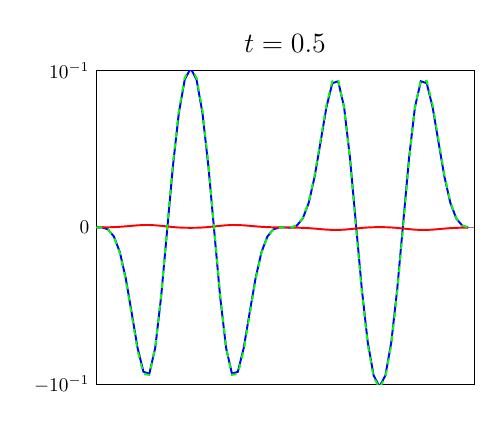
\begin{tikzpicture}[scale=0.7]

\begin{axis}[
    xtick = \empty,
    xmin = 0,
    xmax = 6.2832,
    ymin = -0.1,
    ymax = +0.1,
    ytick = {-0.1,0,0.1},
    yticklabels = {$-10^{-1}$,$0$,$10^{-1}$},
    scaled y ticks = false,
    scaled y ticks = false,
    title = {\Large $t = 0.5$},
  ]

\addplot[blue, line width=1pt] coordinates{
(0.0000e+00,6.0582e-12)
(9.8175e-02,6.4493e-05)
(1.9635e-01,-1.2452e-03)
(2.9452e-01,-5.7788e-03)
(3.9270e-01,-1.5693e-02)
(4.9087e-01,-3.2280e-02)
(5.8905e-01,-5.4213e-02)
(6.8722e-01,-7.6587e-02)
(7.8540e-01,-9.1961e-02)
(8.8357e-01,-9.3196e-02)
(9.8175e-01,-7.6651e-02)
(1.0799e+00,-4.4122e-02)
(1.1781e+00,-2.4484e-03)
(1.2763e+00,3.9226e-02)
(1.3744e+00,7.2989e-02)
(1.4726e+00,9.4253e-02)
(1.5708e+00,1.0142e-01)
(1.6690e+00,9.4253e-02)
(1.7671e+00,7.2989e-02)
(1.8653e+00,3.9226e-02)
(1.9635e+00,-2.4484e-03)
(2.0617e+00,-4.4122e-02)
(2.1598e+00,-7.6651e-02)
(2.2580e+00,-9.3196e-02)
(2.3562e+00,-9.1961e-02)
(2.4544e+00,-7.6587e-02)
(2.5525e+00,-5.4213e-02)
(2.6507e+00,-3.2280e-02)
(2.7489e+00,-1.5693e-02)
(2.8471e+00,-5.7788e-03)
(2.9452e+00,-1.2452e-03)
(3.0434e+00,6.4493e-05)
(3.1416e+00,6.6748e-12)
(3.2398e+00,-6.4493e-05)
(3.3379e+00,1.2452e-03)
(3.4361e+00,5.7788e-03)
(3.5343e+00,1.5693e-02)
(3.6325e+00,3.2280e-02)
(3.7306e+00,5.4213e-02)
(3.8288e+00,7.6587e-02)
(3.9270e+00,9.1961e-02)
(4.0252e+00,9.3196e-02)
(4.1233e+00,7.6651e-02)
(4.2215e+00,4.4122e-02)
(4.3197e+00,2.4484e-03)
(4.4179e+00,-3.9226e-02)
(4.5160e+00,-7.2989e-02)
(4.6142e+00,-9.4253e-02)
(4.7124e+00,-1.0142e-01)
(4.8106e+00,-9.4253e-02)
(4.9087e+00,-7.2989e-02)
(5.0069e+00,-3.9226e-02)
(5.1051e+00,2.4484e-03)
(5.2033e+00,4.4122e-02)
(5.3014e+00,7.6651e-02)
(5.3996e+00,9.3196e-02)
(5.4978e+00,9.1961e-02)
(5.5960e+00,7.6587e-02)
(5.6941e+00,5.4213e-02)
(5.7923e+00,3.2280e-02)
(5.8905e+00,1.5693e-02)
(5.9887e+00,5.7788e-03)
(6.0868e+00,1.2452e-03)
(6.1850e+00,-6.4493e-05)
};

\addplot[red, line width=1pt] coordinates{
(0.0000e+00,6.7339e-18)
(9.8175e-02,4.3333e-05)
(1.9635e-01,1.1058e-04)
(2.9452e-01,2.3031e-04)
(3.9270e-01,4.2984e-04)
(4.9087e-01,7.1540e-04)
(5.8905e-01,1.0514e-03)
(6.8722e-01,1.3614e-03)
(7.8540e-01,1.5567e-03)
(8.8357e-01,1.5722e-03)
(9.8175e-01,1.3903e-03)
(1.0799e+00,1.0511e-03)
(1.1781e+00,6.4307e-04)
(1.2763e+00,2.6721e-04)
(1.3744e+00,-7.6823e-06)
(1.4726e+00,-1.6322e-04)
(1.5708e+00,-2.1189e-04)
(1.6690e+00,-1.6322e-04)
(1.7671e+00,-7.6823e-06)
(1.8653e+00,2.6721e-04)
(1.9635e+00,6.4307e-04)
(2.0617e+00,1.0511e-03)
(2.1598e+00,1.3903e-03)
(2.2580e+00,1.5722e-03)
(2.3562e+00,1.5567e-03)
(2.4544e+00,1.3614e-03)
(2.5525e+00,1.0514e-03)
(2.6507e+00,7.1540e-04)
(2.7489e+00,4.2984e-04)
(2.8471e+00,2.3031e-04)
(2.9452e+00,1.1058e-04)
(3.0434e+00,4.3333e-05)
(3.1416e+00,-2.9592e-17)
(3.2398e+00,-4.3333e-05)
(3.3379e+00,-1.1058e-04)
(3.4361e+00,-2.3031e-04)
(3.5343e+00,-4.2984e-04)
(3.6325e+00,-7.1540e-04)
(3.7306e+00,-1.0514e-03)
(3.8288e+00,-1.3614e-03)
(3.9270e+00,-1.5567e-03)
(4.0252e+00,-1.5722e-03)
(4.1233e+00,-1.3903e-03)
(4.2215e+00,-1.0511e-03)
(4.3197e+00,-6.4307e-04)
(4.4179e+00,-2.6721e-04)
(4.5160e+00,7.6823e-06)
(4.6142e+00,1.6322e-04)
(4.7124e+00,2.1189e-04)
(4.8106e+00,1.6322e-04)
(4.9087e+00,7.6823e-06)
(5.0069e+00,-2.6721e-04)
(5.1051e+00,-6.4307e-04)
(5.2033e+00,-1.0511e-03)
(5.3014e+00,-1.3903e-03)
(5.3996e+00,-1.5722e-03)
(5.4978e+00,-1.5567e-03)
(5.5960e+00,-1.3614e-03)
(5.6941e+00,-1.0514e-03)
(5.7923e+00,-7.1540e-04)
(5.8905e+00,-4.2984e-04)
(5.9887e+00,-2.3031e-04)
(6.0868e+00,-1.1058e-04)
(6.1850e+00,-4.3333e-05)
};

\addplot[green, dashed, line width=1pt] coordinates{
(0.0000e+00,-3.9124e-12)
(9.8175e-02,2.0720e-05)
(1.9635e-01,-1.3715e-03)
(2.9452e-01,-6.0708e-03)
(3.9270e-01,-1.6268e-02)
(4.9087e-01,-3.3236e-02)
(5.8905e-01,-5.5539e-02)
(6.8722e-01,-7.8093e-02)
(7.8540e-01,-9.3289e-02)
(8.8357e-01,-9.3941e-02)
(9.8175e-01,-7.6532e-02)
(1.0799e+00,-4.3130e-02)
(1.1781e+00,-8.7651e-04)
(1.2763e+00,4.0917e-02)
(1.3744e+00,7.4420e-02)
(1.4726e+00,9.5324e-02)
(1.5708e+00,1.0233e-01)
(1.6690e+00,9.5324e-02)
(1.7671e+00,7.4420e-02)
(1.8653e+00,4.0917e-02)
(1.9635e+00,-8.7651e-04)
(2.0617e+00,-4.3130e-02)
(2.1598e+00,-7.6532e-02)
(2.2580e+00,-9.3941e-02)
(2.3562e+00,-9.3289e-02)
(2.4544e+00,-7.8093e-02)
(2.5525e+00,-5.5539e-02)
(2.6507e+00,-3.3236e-02)
(2.7489e+00,-1.6268e-02)
(2.8471e+00,-6.0708e-03)
(2.9452e+00,-1.3715e-03)
(3.0434e+00,2.0720e-05)
(3.1416e+00,5.6502e-13)
(3.2398e+00,-2.0720e-05)
(3.3379e+00,1.3715e-03)
(3.4361e+00,6.0708e-03)
(3.5343e+00,1.6268e-02)
(3.6325e+00,3.3236e-02)
(3.7306e+00,5.5539e-02)
(3.8288e+00,7.8093e-02)
(3.9270e+00,9.3289e-02)
(4.0252e+00,9.3941e-02)
(4.1233e+00,7.6532e-02)
(4.2215e+00,4.3130e-02)
(4.3197e+00,8.7651e-04)
(4.4179e+00,-4.0917e-02)
(4.5160e+00,-7.4420e-02)
(4.6142e+00,-9.5324e-02)
(4.7124e+00,-1.0233e-01)
(4.8106e+00,-9.5324e-02)
(4.9087e+00,-7.4420e-02)
(5.0069e+00,-4.0917e-02)
(5.1051e+00,8.7651e-04)
(5.2033e+00,4.3130e-02)
(5.3014e+00,7.6532e-02)
(5.3996e+00,9.3941e-02)
(5.4978e+00,9.3289e-02)
(5.5960e+00,7.8093e-02)
(5.6941e+00,5.5539e-02)
(5.7923e+00,3.3236e-02)
(5.8905e+00,1.6268e-02)
(5.9887e+00,6.0708e-03)
(6.0868e+00,1.3715e-03)
(6.1850e+00,-2.0720e-05)
};

\end{axis}



\end{tikzpicture}

%  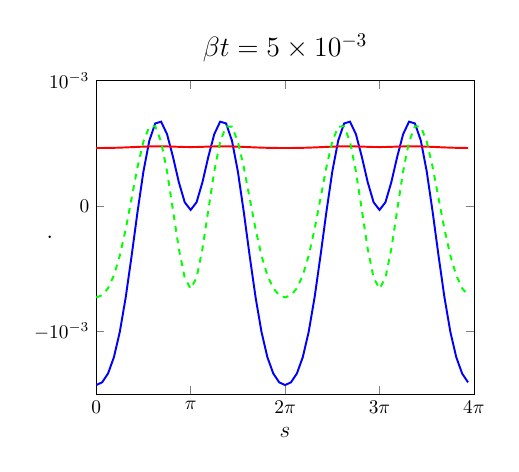
\begin{tikzpicture}[scale=0.7]

\begin{axis}[
    xmin = 0,
    xmax = 6.2832,
    xtick = {0,1.5708,3.1416,4.7124,6.2832},
    xticklabels = {$0$, $\pi$, $2\pi$, $3\pi$, $4\pi$},
    xlabel = {\large $s$},
    ymin = -0.0015,
    ymax = +0.001,
    ytick = {-0.001,0,0.001},
    yticklabels = {$-10^{-3}$,$0$,$10^{-3}$},
    ylabel = {\large $\uu \cdot \nn$},
    ylabel near ticks,
    ylabel shift = {-18pt},
    scaled y ticks = false,
    title = {\Large $\beta t = 5 \times 10^{-3}$},
  ]

\addplot[blue, line width=1pt] coordinates{
(0.0000e+00,-1.4252e-03)
(9.8175e-02,-1.4035e-03)
(1.9635e-01,-1.3334e-03)
(2.9452e-01,-1.2031e-03)
(3.9270e-01,-1.0011e-03)
(4.9087e-01,-7.2625e-04)
(5.8905e-01,-3.9562e-04)
(6.8722e-01,-4.5522e-05)
(7.8540e-01,2.7595e-04)
(8.8357e-01,5.2203e-04)
(9.8175e-01,6.5904e-04)
(1.0799e+00,6.7307e-04)
(1.1781e+00,5.7336e-04)
(1.2763e+00,3.9382e-04)
(1.3744e+00,1.9062e-04)
(1.4726e+00,3.0662e-05)
(1.5708e+00,-3.0007e-05)
(1.6690e+00,3.0662e-05)
(1.7671e+00,1.9062e-04)
(1.8653e+00,3.9382e-04)
(1.9635e+00,5.7336e-04)
(2.0617e+00,6.7307e-04)
(2.1598e+00,6.5904e-04)
(2.2580e+00,5.2203e-04)
(2.3562e+00,2.7595e-04)
(2.4544e+00,-4.5522e-05)
(2.5525e+00,-3.9562e-04)
(2.6507e+00,-7.2625e-04)
(2.7489e+00,-1.0011e-03)
(2.8471e+00,-1.2031e-03)
(2.9452e+00,-1.3334e-03)
(3.0434e+00,-1.4035e-03)
(3.1416e+00,-1.4252e-03)
(3.2398e+00,-1.4035e-03)
(3.3379e+00,-1.3334e-03)
(3.4361e+00,-1.2031e-03)
(3.5343e+00,-1.0011e-03)
(3.6325e+00,-7.2625e-04)
(3.7306e+00,-3.9562e-04)
(3.8288e+00,-4.5522e-05)
(3.9270e+00,2.7595e-04)
(4.0252e+00,5.2203e-04)
(4.1233e+00,6.5904e-04)
(4.2215e+00,6.7307e-04)
(4.3197e+00,5.7336e-04)
(4.4179e+00,3.9382e-04)
(4.5160e+00,1.9062e-04)
(4.6142e+00,3.0662e-05)
(4.7124e+00,-3.0007e-05)
(4.8106e+00,3.0662e-05)
(4.9087e+00,1.9062e-04)
(5.0069e+00,3.9382e-04)
(5.1051e+00,5.7336e-04)
(5.2033e+00,6.7307e-04)
(5.3014e+00,6.5904e-04)
(5.3996e+00,5.2203e-04)
(5.4978e+00,2.7595e-04)
(5.5960e+00,-4.5522e-05)
(5.6941e+00,-3.9562e-04)
(5.7923e+00,-7.2625e-04)
(5.8905e+00,-1.0011e-03)
(5.9887e+00,-1.2031e-03)
(6.0868e+00,-1.3334e-03)
(6.1850e+00,-1.4035e-03)
};

\addplot[red, line width=1pt] coordinates{
(0.0000e+00,4.6324e-04)
(9.8175e-02,4.6339e-04)
(1.9635e-01,4.6387e-04)
(2.9452e-01,4.6475e-04)
(3.9270e-01,4.6609e-04)
(4.9087e-01,4.6787e-04)
(5.8905e-01,4.6994e-04)
(6.8722e-01,4.7207e-04)
(7.8540e-01,4.7399e-04)
(8.8357e-01,4.7546e-04)
(9.8175e-01,4.7630e-04)
(1.0799e+00,4.7637e-04)
(1.1781e+00,4.7565e-04)
(1.2763e+00,4.7429e-04)
(1.3744e+00,4.7265e-04)
(1.4726e+00,4.7130e-04)
(1.5708e+00,4.7077e-04)
(1.6690e+00,4.7130e-04)
(1.7671e+00,4.7265e-04)
(1.8653e+00,4.7429e-04)
(1.9635e+00,4.7565e-04)
(2.0617e+00,4.7637e-04)
(2.1598e+00,4.7630e-04)
(2.2580e+00,4.7546e-04)
(2.3562e+00,4.7399e-04)
(2.4544e+00,4.7207e-04)
(2.5525e+00,4.6994e-04)
(2.6507e+00,4.6787e-04)
(2.7489e+00,4.6609e-04)
(2.8471e+00,4.6475e-04)
(2.9452e+00,4.6387e-04)
(3.0434e+00,4.6339e-04)
(3.1416e+00,4.6324e-04)
(3.2398e+00,4.6339e-04)
(3.3379e+00,4.6387e-04)
(3.4361e+00,4.6475e-04)
(3.5343e+00,4.6609e-04)
(3.6325e+00,4.6787e-04)
(3.7306e+00,4.6994e-04)
(3.8288e+00,4.7207e-04)
(3.9270e+00,4.7399e-04)
(4.0252e+00,4.7546e-04)
(4.1233e+00,4.7630e-04)
(4.2215e+00,4.7637e-04)
(4.3197e+00,4.7565e-04)
(4.4179e+00,4.7429e-04)
(4.5160e+00,4.7265e-04)
(4.6142e+00,4.7130e-04)
(4.7124e+00,4.7077e-04)
(4.8106e+00,4.7130e-04)
(4.9087e+00,4.7265e-04)
(5.0069e+00,4.7429e-04)
(5.1051e+00,4.7565e-04)
(5.2033e+00,4.7637e-04)
(5.3014e+00,4.7630e-04)
(5.3996e+00,4.7546e-04)
(5.4978e+00,4.7399e-04)
(5.5960e+00,4.7207e-04)
(5.6941e+00,4.6994e-04)
(5.7923e+00,4.6787e-04)
(5.8905e+00,4.6609e-04)
(5.9887e+00,4.6475e-04)
(6.0868e+00,4.6387e-04)
(6.1850e+00,4.6339e-04)
};

\addplot[green, dashed, line width=1pt] coordinates{
(0.0000e+00,-7.2674e-04)
(9.8175e-02,-7.0951e-04)
(1.9635e-01,-6.5403e-04)
(2.9452e-01,-5.5135e-04)
(3.9270e-01,-3.9376e-04)
(4.9087e-01,-1.8298e-04)
(5.8905e-01,6.3302e-05)
(6.8722e-01,3.1063e-04)
(7.8540e-01,5.1478e-04)
(8.8357e-01,6.3332e-04)
(9.8175e-01,6.3615e-04)
(1.0799e+00,5.1265e-04)
(1.1781e+00,2.7661e-04)
(1.2763e+00,-3.0169e-05)
(1.3744e+00,-3.3971e-04)
(1.4726e+00,-5.7126e-04)
(1.5708e+00,-6.5729e-04)
(1.6690e+00,-5.7126e-04)
(1.7671e+00,-3.3971e-04)
(1.8653e+00,-3.0169e-05)
(1.9635e+00,2.7661e-04)
(2.0617e+00,5.1265e-04)
(2.1598e+00,6.3615e-04)
(2.2580e+00,6.3332e-04)
(2.3562e+00,5.1478e-04)
(2.4544e+00,3.1063e-04)
(2.5525e+00,6.3302e-05)
(2.6507e+00,-1.8298e-04)
(2.7489e+00,-3.9376e-04)
(2.8471e+00,-5.5135e-04)
(2.9452e+00,-6.5403e-04)
(3.0434e+00,-7.0951e-04)
(3.1416e+00,-7.2674e-04)
(3.2398e+00,-7.0951e-04)
(3.3379e+00,-6.5403e-04)
(3.4361e+00,-5.5135e-04)
(3.5343e+00,-3.9376e-04)
(3.6325e+00,-1.8298e-04)
(3.7306e+00,6.3302e-05)
(3.8288e+00,3.1063e-04)
(3.9270e+00,5.1478e-04)
(4.0252e+00,6.3332e-04)
(4.1233e+00,6.3615e-04)
(4.2215e+00,5.1265e-04)
(4.3197e+00,2.7661e-04)
(4.4179e+00,-3.0169e-05)
(4.5160e+00,-3.3971e-04)
(4.6142e+00,-5.7126e-04)
(4.7124e+00,-6.5729e-04)
(4.8106e+00,-5.7126e-04)
(4.9087e+00,-3.3971e-04)
(5.0069e+00,-3.0169e-05)
(5.1051e+00,2.7661e-04)
(5.2033e+00,5.1265e-04)
(5.3014e+00,6.3615e-04)
(5.3996e+00,6.3332e-04)
(5.4978e+00,5.1478e-04)
(5.5960e+00,3.1063e-04)
(5.6941e+00,6.3302e-05)
(5.7923e+00,-1.8298e-04)
(5.8905e+00,-3.9376e-04)
(5.9887e+00,-5.5135e-04)
(6.0868e+00,-6.5403e-04)
(6.1850e+00,-7.0951e-04)
};

\end{axis}


\end{tikzpicture}

%  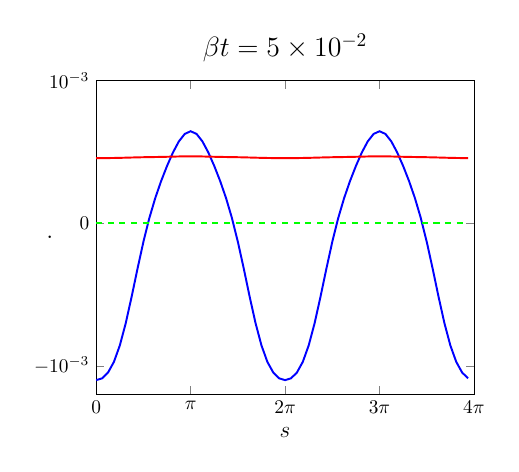
\begin{tikzpicture}[scale=0.7]


\begin{axis}[
    xmin = 0,
    xmax = 6.2832,
    xtick = {0,1.5708,3.1416,4.7124,6.2832},
    xticklabels = {$0$, $\pi$, $2\pi$, $3\pi$, $4\pi$},
    xlabel = {\large $s$},
    ymin = -0.0012,
    ymax = +0.001,
    ytick = {-0.001,0,0.001},
    yticklabels = {$-10^{-3}$,$0$,$10^{-3}$},
    ylabel = {\large $\uu \cdot \nn$},
    ylabel near ticks,
    ylabel shift = {-18pt},
    scaled y ticks = false,
    title = {\Large $\beta t = 5 \times 10^{-2}$},
  ]

\addplot[blue, line width=1pt] coordinates{
(0.0000e+00,-1.0996e-03)
(9.8175e-02,-1.0870e-03)
(1.9635e-01,-1.0466e-03)
(2.9452e-01,-9.7170e-04)
(3.9270e-01,-8.5638e-04)
(4.9087e-01,-7.0082e-04)
(5.8905e-01,-5.1507e-04)
(6.8722e-01,-3.1782e-04)
(7.8540e-01,-1.2954e-04)
(8.8357e-01,3.6091e-05)
(9.8175e-01,1.7622e-04)
(1.0799e+00,2.9597e-04)
(1.1781e+00,4.0183e-04)
(1.2763e+00,4.9586e-04)
(1.3744e+00,5.7370e-04)
(1.4726e+00,6.2639e-04)
(1.5708e+00,6.4517e-04)
(1.6690e+00,6.2639e-04)
(1.7671e+00,5.7370e-04)
(1.8653e+00,4.9586e-04)
(1.9635e+00,4.0183e-04)
(2.0617e+00,2.9597e-04)
(2.1598e+00,1.7622e-04)
(2.2580e+00,3.6091e-05)
(2.3562e+00,-1.2954e-04)
(2.4544e+00,-3.1782e-04)
(2.5525e+00,-5.1507e-04)
(2.6507e+00,-7.0082e-04)
(2.7489e+00,-8.5638e-04)
(2.8471e+00,-9.7170e-04)
(2.9452e+00,-1.0466e-03)
(3.0434e+00,-1.0870e-03)
(3.1416e+00,-1.0996e-03)
(3.2398e+00,-1.0870e-03)
(3.3379e+00,-1.0466e-03)
(3.4361e+00,-9.7170e-04)
(3.5343e+00,-8.5638e-04)
(3.6325e+00,-7.0082e-04)
(3.7306e+00,-5.1507e-04)
(3.8288e+00,-3.1782e-04)
(3.9270e+00,-1.2954e-04)
(4.0252e+00,3.6091e-05)
(4.1233e+00,1.7622e-04)
(4.2215e+00,2.9597e-04)
(4.3197e+00,4.0183e-04)
(4.4179e+00,4.9586e-04)
(4.5160e+00,5.7370e-04)
(4.6142e+00,6.2639e-04)
(4.7124e+00,6.4517e-04)
(4.8106e+00,6.2639e-04)
(4.9087e+00,5.7370e-04)
(5.0069e+00,4.9586e-04)
(5.1051e+00,4.0183e-04)
(5.2033e+00,2.9597e-04)
(5.3014e+00,1.7622e-04)
(5.3996e+00,3.6091e-05)
(5.4978e+00,-1.2954e-04)
(5.5960e+00,-3.1782e-04)
(5.6941e+00,-5.1507e-04)
(5.7923e+00,-7.0082e-04)
(5.8905e+00,-8.5638e-04)
(5.9887e+00,-9.7170e-04)
(6.0868e+00,-1.0466e-03)
(6.1850e+00,-1.0870e-03)
};

\addplot[red, line width=1pt] coordinates{
(0.0000e+00,4.5667e-04)
(9.8175e-02,4.5678e-04)
(1.9635e-01,4.5711e-04)
(2.9452e-01,4.5772e-04)
(3.9270e-01,4.5862e-04)
(4.9087e-01,4.5975e-04)
(5.8905e-01,4.6097e-04)
(6.8722e-01,4.6210e-04)
(7.8540e-01,4.6302e-04)
(8.8357e-01,4.6376e-04)
(9.8175e-01,4.6444e-04)
(1.0799e+00,4.6521e-04)
(1.1781e+00,4.6616e-04)
(1.2763e+00,4.6723e-04)
(1.3744e+00,4.6829e-04)
(1.4726e+00,4.6908e-04)
(1.5708e+00,4.6938e-04)
(1.6690e+00,4.6908e-04)
(1.7671e+00,4.6829e-04)
(1.8653e+00,4.6723e-04)
(1.9635e+00,4.6616e-04)
(2.0617e+00,4.6521e-04)
(2.1598e+00,4.6444e-04)
(2.2580e+00,4.6376e-04)
(2.3562e+00,4.6302e-04)
(2.4544e+00,4.6210e-04)
(2.5525e+00,4.6097e-04)
(2.6507e+00,4.5975e-04)
(2.7489e+00,4.5862e-04)
(2.8471e+00,4.5772e-04)
(2.9452e+00,4.5711e-04)
(3.0434e+00,4.5678e-04)
(3.1416e+00,4.5667e-04)
(3.2398e+00,4.5678e-04)
(3.3379e+00,4.5711e-04)
(3.4361e+00,4.5772e-04)
(3.5343e+00,4.5862e-04)
(3.6325e+00,4.5975e-04)
(3.7306e+00,4.6097e-04)
(3.8288e+00,4.6210e-04)
(3.9270e+00,4.6302e-04)
(4.0252e+00,4.6376e-04)
(4.1233e+00,4.6444e-04)
(4.2215e+00,4.6521e-04)
(4.3197e+00,4.6616e-04)
(4.4179e+00,4.6723e-04)
(4.5160e+00,4.6829e-04)
(4.6142e+00,4.6908e-04)
(4.7124e+00,4.6938e-04)
(4.8106e+00,4.6908e-04)
(4.9087e+00,4.6829e-04)
(5.0069e+00,4.6723e-04)
(5.1051e+00,4.6616e-04)
(5.2033e+00,4.6521e-04)
(5.3014e+00,4.6444e-04)
(5.3996e+00,4.6376e-04)
(5.4978e+00,4.6302e-04)
(5.5960e+00,4.6210e-04)
(5.6941e+00,4.6097e-04)
(5.7923e+00,4.5975e-04)
(5.8905e+00,4.5862e-04)
(5.9887e+00,4.5772e-04)
(6.0868e+00,4.5711e-04)
(6.1850e+00,4.5678e-04)
};

\addplot[green, dashed, line width=1pt] coordinates{
(0.0000e+00,-2.3701e-12)
(9.8175e-02,-5.1013e-12)
(1.9635e-01,-2.1890e-12)
(2.9452e-01,-3.5219e-12)
(3.9270e-01,-1.5410e-12)
(4.9087e-01,-1.8243e-12)
(5.8905e-01,-4.6256e-13)
(6.8722e-01,8.3140e-13)
(7.8540e-01,1.0570e-12)
(8.8357e-01,2.3248e-12)
(9.8175e-01,2.1470e-12)
(1.0799e+00,3.2332e-12)
(1.1781e+00,2.3841e-12)
(1.2763e+00,3.6752e-12)
(1.3744e+00,2.7500e-12)
(1.4726e+00,3.8911e-12)
(1.5708e+00,3.0465e-12)
(1.6690e+00,3.7839e-12)
(1.7671e+00,2.9670e-12)
(1.8653e+00,3.3832e-12)
(1.9635e+00,2.5833e-12)
(2.0617e+00,3.1272e-12)
(2.1598e+00,1.9943e-12)
(2.2580e+00,2.8072e-12)
(2.3562e+00,4.5835e-13)
(2.4544e+00,1.8049e-12)
(2.5525e+00,-1.7784e-12)
(2.6507e+00,4.5430e-13)
(2.7489e+00,-4.4271e-12)
(2.8471e+00,-1.2356e-12)
(2.9452e+00,-4.6053e-12)
(3.0434e+00,-2.1283e-12)
(3.1416e+00,-5.5059e-12)
(3.2398e+00,-3.2576e-12)
(3.3379e+00,-2.5917e-12)
(3.4361e+00,-3.6846e-12)
(3.5343e+00,-1.2203e-12)
(3.6325e+00,-2.5257e-12)
(3.7306e+00,4.3051e-13)
(3.8288e+00,-1.0295e-13)
(3.9270e+00,2.0464e-12)
(4.0252e+00,1.3831e-12)
(4.1233e+00,3.1439e-12)
(4.2215e+00,2.1068e-12)
(4.3197e+00,3.5191e-12)
(4.4179e+00,2.5897e-12)
(4.5160e+00,3.8035e-12)
(4.6142e+00,2.9385e-12)
(4.7124e+00,3.9496e-12)
(4.8106e+00,2.9646e-12)
(4.9087e+00,3.7350e-12)
(5.0069e+00,2.6137e-12)
(5.1051e+00,3.3981e-12)
(5.2033e+00,2.3594e-12)
(5.3014e+00,2.9610e-12)
(5.3996e+00,1.6281e-12)
(5.4978e+00,1.7719e-12)
(5.5960e+00,1.6160e-13)
(5.6941e+00,-2.2854e-13)
(5.7923e+00,-1.1349e-12)
(5.8905e+00,-2.8796e-12)
(5.9887e+00,-2.9905e-12)
(6.0868e+00,-2.1672e-12)
(6.1850e+00,-5.0508e-12)
};

\end{axis}

\end{tikzpicture}

%  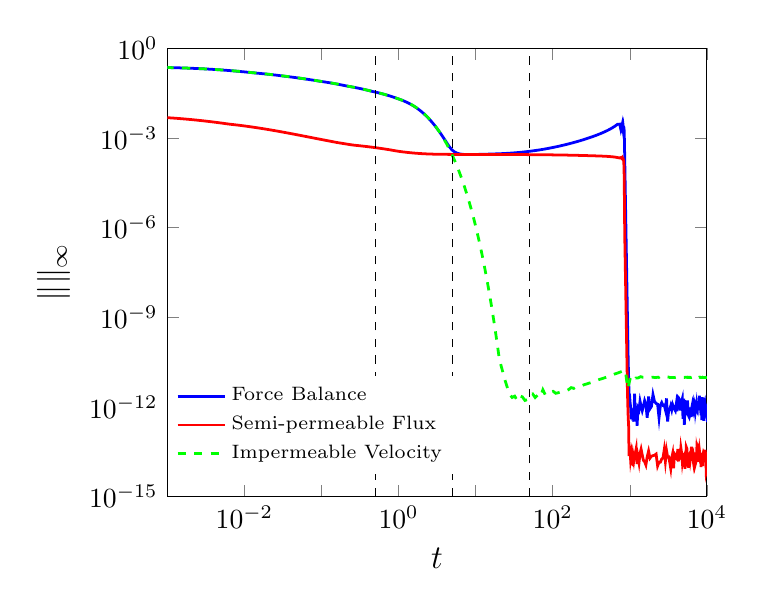
\begin{tikzpicture}[scale=1]

  \begin{axis}[
    name = maxPlot,
    xmin = 1e-3,
    xmax = 10000,
    ymin = 1e-15,
    ymax = 1e0,
    xmode = log,
    ymode = log,
    xminorticks = false,
    yminorticks = false,
    xtick = {1e-3,1e-2,1e-1,1e0,1e1,1e2,1e3,1e4},
    xticklabels = {,$10^{-2}$,,$10^0$,,$10^2$,,$10^4$},
    xlabel = {\large $t$},
    ylabel = {\large $\|\uu\|_\infty$},
    ylabel near ticks,
    legend entries = {Force Balance,
    Semi-permeable Flux,Impermeable Velocity},
    legend cell align=left,
    legend style={draw=none,font=\scriptsize},
    legend style={at={(0.0,0.05)},anchor=south west}
  ]

\addplot[blue, line width=1pt] coordinates{
(0.0000e+00,2.5143e-01)
(6.4149e-05,2.4906e-01)
(1.2188e-04,2.4693e-01)
(1.8424e-04,2.4478e-01)
(2.5158e-04,2.4254e-01)
(3.2431e-04,2.4022e-01)
(4.0286e-04,2.3783e-01)
(4.8769e-04,2.3537e-01)
(5.7930e-04,2.3284e-01)
(6.7825e-04,2.3024e-01)
(7.8511e-04,2.2773e-01)
(9.0052e-04,2.2619e-01)
(1.0252e-03,2.2455e-01)
(1.1598e-03,2.2283e-01)
(1.3052e-03,2.2100e-01)
(1.4622e-03,2.1908e-01)
(1.6318e-03,2.1706e-01)
(1.8149e-03,2.1494e-01)
(2.0127e-03,2.1273e-01)
(2.2263e-03,2.1043e-01)
(2.4570e-03,2.0804e-01)
(2.7062e-03,2.0557e-01)
(2.9753e-03,2.0301e-01)
(3.2659e-03,2.0037e-01)
(3.5798e-03,1.9766e-01)
(3.9188e-03,1.9487e-01)
(4.2849e-03,1.9201e-01)
(4.6803e-03,1.8909e-01)
(5.1073e-03,1.8610e-01)
(5.5685e-03,1.8306e-01)
(6.0666e-03,1.7997e-01)
(6.6045e-03,1.7683e-01)
(7.1855e-03,1.7365e-01)
(7.8129e-03,1.7043e-01)
(8.4905e-03,1.6718e-01)
(9.2224e-03,1.6390e-01)
(9.9991e-03,1.6066e-01)
(1.0827e-02,1.5743e-01)
(1.1702e-02,1.5426e-01)
(1.2641e-02,1.5108e-01)
(1.3621e-02,1.4800e-01)
(1.4679e-02,1.4543e-01)
(1.5779e-02,1.4296e-01)
(1.6968e-02,1.4043e-01)
(1.8208e-02,1.3794e-01)
(1.9547e-02,1.3539e-01)
(2.0933e-02,1.3290e-01)
(2.2430e-02,1.3035e-01)
(2.3996e-02,1.2782e-01)
(2.5687e-02,1.2523e-01)
(2.7422e-02,1.2273e-01)
(2.9295e-02,1.2015e-01)
(3.1276e-02,1.1758e-01)
(3.3376e-02,1.1510e-01)
(3.5593e-02,1.1281e-01)
(3.7949e-02,1.1053e-01)
(4.0425e-02,1.0827e-01)
(4.3074e-02,1.0599e-01)
(4.5826e-02,1.0377e-01)
(4.8797e-02,1.0149e-01)
(5.1865e-02,9.9283e-02)
(5.5178e-02,9.7024e-02)
(5.8630e-02,9.4806e-02)
(6.2358e-02,9.2538e-02)
(6.6187e-02,9.0543e-02)
(7.0322e-02,8.8527e-02)
(7.4666e-02,8.6516e-02)
(7.9318e-02,8.4459e-02)
(8.4141e-02,8.2434e-02)
(8.9350e-02,8.0349e-02)
(9.4748e-02,7.8401e-02)
(1.0058e-01,7.6656e-02)
(1.0663e-01,7.4942e-02)
(1.1316e-01,7.3178e-02)
(1.1994e-01,7.1447e-02)
(1.2725e-01,6.9669e-02)
(1.3486e-01,6.7918e-02)
(1.4308e-01,6.6121e-02)
(1.5159e-01,6.4360e-02)
(1.6079e-01,6.2557e-02)
(1.7039e-01,6.0778e-02)
(1.8076e-01,5.8961e-02)
(1.9148e-01,5.7215e-02)
(2.0304e-01,5.5535e-02)
(2.1521e-01,5.3906e-02)
(2.2829e-01,5.2503e-02)
(2.4187e-01,5.1119e-02)
(2.5654e-01,4.9696e-02)
(2.7191e-01,4.8285e-02)
(2.8850e-01,4.6839e-02)
(3.0579e-01,4.5415e-02)
(3.2446e-01,4.3960e-02)
(3.4425e-01,4.2507e-02)
(3.6555e-01,4.1032e-02)
(3.8802e-01,3.9571e-02)
(4.1229e-01,3.8090e-02)
(4.3823e-01,3.6663e-02)
(4.6618e-01,3.5256e-02)
(4.9600e-01,3.4003e-02)
(5.2821e-01,3.2752e-02)
(5.6259e-01,3.1488e-02)
(5.9972e-01,3.0196e-02)
(6.3901e-01,2.8902e-02)
(6.8145e-01,2.7582e-02)
(7.2600e-01,2.6334e-02)
(7.7412e-01,2.5064e-02)
(8.2397e-01,2.3816e-02)
(8.7782e-01,2.2537e-02)
(9.3363e-01,2.1296e-02)
(9.9391e-01,2.0088e-02)
(1.0560e+00,1.8988e-02)
(1.1231e+00,1.7874e-02)
(1.1935e+00,1.6761e-02)
(1.2696e+00,1.5602e-02)
(1.3493e+00,1.4457e-02)
(1.4353e+00,1.3282e-02)
(1.5282e+00,1.2101e-02)
(1.6286e+00,1.0921e-02)
(1.7370e+00,9.7569e-03)
(1.8540e+00,8.6206e-03)
(1.9805e+00,7.5269e-03)
(2.1170e+00,6.4886e-03)
(2.2645e+00,5.5180e-03)
(2.4237e+00,4.6252e-03)
(2.5957e+00,3.8178e-03)
(2.7815e+00,3.1018e-03)
(2.9821e+00,2.4840e-03)
(3.1988e+00,1.9590e-03)
(3.4328e+00,1.5197e-03)
(3.6855e+00,1.1615e-03)
(3.9584e+00,8.7926e-04)
(4.2532e+00,6.5945e-04)
(4.5716e+00,4.9988e-04)
(4.9154e+00,3.9480e-04)
(5.2868e+00,3.4142e-04)
(5.6878e+00,3.0992e-04)
(6.1209e+00,2.9209e-04)
(6.5887e+00,2.8332e-04)
(7.0939e+00,2.7818e-04)
(7.6395e+00,2.7687e-04)
(8.2288e+00,2.7653e-04)
(8.8652e+00,2.7680e-04)
(9.5525e+00,2.7748e-04)
(1.0295e+01,2.7843e-04)
(1.1096e+01,2.7956e-04)
(1.1962e+01,2.8085e-04)
(1.2897e+01,2.8227e-04)
(1.3907e+01,2.8381e-04)
(1.4998e+01,2.8549e-04)
(1.6176e+01,2.8731e-04)
(1.7448e+01,2.8927e-04)
(1.8822e+01,2.9140e-04)
(2.0306e+01,2.9371e-04)
(2.1908e+01,2.9620e-04)
(2.3639e+01,2.9906e-04)
(2.5509e+01,3.0232e-04)
(2.7527e+01,3.0615e-04)
(2.9708e+01,3.1030e-04)
(3.2062e+01,3.1485e-04)
(3.4605e+01,3.2004e-04)
(3.7352e+01,3.2577e-04)
(4.0318e+01,3.3238e-04)
(4.3522e+01,3.3966e-04)
(4.6982e+01,3.4754e-04)
(5.0718e+01,3.5606e-04)
(5.4754e+01,3.6529e-04)
(5.9112e+01,3.7527e-04)
(6.3819e+01,3.8609e-04)
(6.8903e+01,3.9780e-04)
(7.4393e+01,4.1106e-04)
(8.0323e+01,4.2566e-04)
(8.6727e+01,4.4148e-04)
(9.3643e+01,4.5860e-04)
(1.0111e+02,4.7716e-04)
(1.0918e+02,4.9728e-04)
(1.1789e+02,5.1910e-04)
(1.2730e+02,5.4279e-04)
(1.3746e+02,5.6851e-04)
(1.4844e+02,5.9648e-04)
(1.6029e+02,6.2690e-04)
(1.7309e+02,6.6004e-04)
(1.8692e+02,6.9619e-04)
(2.0185e+02,7.3567e-04)
(2.1798e+02,7.7888e-04)
(2.3539e+02,8.2627e-04)
(2.5420e+02,8.7860e-04)
(2.7452e+02,9.3646e-04)
(2.9646e+02,1.0004e-03)
(3.2015e+02,1.0713e-03)
(3.4574e+02,1.1504e-03)
(3.7338e+02,1.2392e-03)
(4.0323e+02,1.3396e-03)
(4.3546e+02,1.4544e-03)
(4.7028e+02,1.5874e-03)
(5.0788e+02,1.7443e-03)
(5.4849e+02,1.9321e-03)
(5.9234e+02,2.1625e-03)
(6.3971e+02,2.4532e-03)
(6.9087e+02,2.8309e-03)
(7.3860e+02,2.8717e-03)
(7.6471e+02,1.8870e-03)
(7.8821e+02,2.5831e-03)
(7.9978e+02,1.5132e-03)
(8.1019e+02,2.1951e-03)
(8.1786e+02,1.8397e-03)
(8.2476e+02,2.1848e-03)
(8.2894e+02,1.9639e-03)
(8.3270e+02,2.1935e-03)
(8.3676e+02,2.1955e-03)
(8.4008e+02,2.0963e-03)
(8.4307e+02,1.8359e-03)
(8.4630e+02,1.3692e-03)
(8.4979e+02,8.5321e-04)
(8.5355e+02,4.6151e-04)
(8.5762e+02,2.2880e-04)
(8.6201e+02,1.0623e-04)
(8.6676e+02,4.6574e-05)
(8.7188e+02,1.9205e-05)
(8.7741e+02,7.4416e-06)
(8.8339e+02,2.6891e-06)
(8.8984e+02,9.0581e-07)
(8.9681e+02,2.8105e-07)
(9.0434e+02,8.0677e-08)
(9.1247e+02,2.0930e-08)
(9.2125e+02,5.0195e-09)
(9.3074e+02,1.0411e-09)
(9.4098e+02,2.1553e-10)
(9.5204e+02,3.3127e-11)
(9.6399e+02,1.0173e-11)
(9.7689e+02,2.6156e-12)
(9.9082e+02,2.5647e-12)
(1.0059e+03,1.4604e-12)
(1.0221e+03,1.0297e-12)
(1.0397e+03,3.8532e-13)
(1.0586e+03,8.7966e-13)
(1.0791e+03,5.6448e-13)
(1.1012e+03,6.7332e-13)
(1.1251e+03,3.1864e-13)
(1.1509e+03,2.7655e-12)
(1.1787e+03,4.3047e-13)
(1.2088e+03,9.2874e-13)
(1.2413e+03,2.3389e-13)
(1.2764e+03,9.1925e-13)
(1.3143e+03,7.9248e-13)
(1.3552e+03,1.5394e-12)
(1.3994e+03,1.0368e-12)
(1.4472e+03,7.4452e-13)
(1.4987e+03,1.0463e-12)
(1.5544e+03,1.6068e-12)
(1.6145e+03,1.2030e-12)
(1.6795e+03,4.3113e-13)
(1.7496e+03,2.2264e-12)
(1.8254e+03,8.6291e-13)
(1.9072e+03,1.0332e-12)
(1.9955e+03,2.5592e-12)
(2.0910e+03,1.4926e-12)
(2.1910e+03,1.3019e-12)
(2.2910e+03,1.2244e-12)
(2.3910e+03,4.2932e-13)
(2.4910e+03,1.1290e-12)
(2.5910e+03,1.3855e-12)
(2.6910e+03,1.1209e-12)
(2.7910e+03,1.1519e-12)
(2.8910e+03,7.9919e-13)
(2.9910e+03,1.9182e-12)
(3.0910e+03,3.2355e-13)
(3.1910e+03,7.8306e-13)
(3.2910e+03,8.0543e-13)
(3.3910e+03,1.0720e-12)
(3.4910e+03,7.9869e-13)
(3.5910e+03,1.1848e-12)
(3.6910e+03,9.7610e-13)
(3.7910e+03,8.4733e-13)
(3.8910e+03,7.4753e-13)
(3.9910e+03,1.1734e-12)
(4.0910e+03,7.0933e-13)
(4.1910e+03,2.1420e-12)
(4.2910e+03,2.0005e-12)
(4.3910e+03,1.7126e-12)
(4.4910e+03,8.2398e-13)
(4.5910e+03,8.2245e-13)
(4.6910e+03,1.5379e-12)
(4.7910e+03,1.8778e-12)
(4.8910e+03,3.9299e-13)
(4.9910e+03,1.8851e-12)
(5.0910e+03,2.5074e-13)
(5.1910e+03,9.8207e-13)
(5.2910e+03,9.0016e-13)
(5.3910e+03,1.6474e-12)
(5.4910e+03,5.2017e-13)
(5.5910e+03,1.6420e-12)
(5.6910e+03,7.9097e-13)
(5.7910e+03,4.9046e-13)
(5.8910e+03,4.4748e-13)
(5.9910e+03,5.4278e-13)
(6.0910e+03,9.5033e-13)
(6.1910e+03,4.5112e-13)
(6.2910e+03,8.8500e-13)
(6.3910e+03,1.0037e-12)
(6.4910e+03,1.2334e-12)
(6.5910e+03,9.5577e-13)
(6.6910e+03,1.4078e-12)
(6.7910e+03,4.8365e-13)
(6.8910e+03,1.3804e-12)
(6.9910e+03,1.2211e-12)
(7.0910e+03,7.2179e-13)
(7.1910e+03,9.3724e-13)
(7.2910e+03,1.1978e-12)
(7.3910e+03,7.6460e-13)
(7.4910e+03,7.1138e-13)
(7.5910e+03,1.4478e-12)
(7.6910e+03,9.7540e-13)
(7.7910e+03,9.4444e-13)
(7.8910e+03,7.7455e-13)
(7.9910e+03,2.3758e-12)
(8.0910e+03,1.3559e-12)
(8.1910e+03,8.2851e-13)
(8.2910e+03,7.7395e-13)
(8.3910e+03,5.2508e-13)
(8.4910e+03,1.5877e-12)
(8.5910e+03,3.6241e-13)
(8.6910e+03,2.0898e-12)
(8.7910e+03,1.1283e-12)
(8.8910e+03,5.7107e-13)
(8.9910e+03,8.8000e-13)
(9.0910e+03,3.4033e-13)
(9.1910e+03,1.9988e-12)
(9.2910e+03,1.2492e-12)
(9.3910e+03,1.3974e-12)
(9.4910e+03,1.1016e-12)
(9.5910e+03,8.3162e-13)
(9.6910e+03,9.6957e-13)
(9.7910e+03,9.9004e-13)
(9.8910e+03,1.1992e-12)
(9.9910e+03,7.0748e-13)
(1.0091e+04,8.0575e-13)
(1.0191e+04,4.0864e-13)
(1.0291e+04,3.1129e-13)
(1.0391e+04,5.2996e-13)
(1.0491e+04,2.2481e-12)
(1.0591e+04,7.9016e-13)
(1.0691e+04,9.1354e-13)
(1.0791e+04,4.7389e-13)
(1.0891e+04,6.1893e-13)
(1.0991e+04,1.8346e-12)
(1.1091e+04,1.5432e-12)
(1.1191e+04,9.1388e-13)
(1.1291e+04,8.0937e-13)
(1.1391e+04,1.5291e-12)
(1.1491e+04,8.5536e-13)
(1.1591e+04,1.9577e-12)
(1.1691e+04,8.2352e-13)
(1.1791e+04,1.0942e-12)
(1.1891e+04,9.8388e-13)
(1.1991e+04,1.6554e-12)
(1.2091e+04,1.3927e-12)
(1.2191e+04,9.2175e-13)
(1.2291e+04,1.0800e-12)
(1.2391e+04,6.8912e-13)
(1.2491e+04,6.7045e-13)
(1.2591e+04,1.3170e-12)
(1.2691e+04,1.0000e-12)
(1.2791e+04,6.0368e-13)
(1.2891e+04,4.6551e-13)
(1.2991e+04,4.2708e-13)
(1.3091e+04,7.9265e-13)
(1.3191e+04,1.0978e-12)
(1.3291e+04,1.0257e-12)
(1.3391e+04,5.0769e-13)
(1.3491e+04,1.4083e-12)
(1.3591e+04,8.9094e-13)
(1.3691e+04,1.4698e-12)
(1.3791e+04,9.7415e-13)
(1.3891e+04,8.7689e-13)
(1.3991e+04,6.3129e-13)
(1.4091e+04,7.5509e-13)
(1.4191e+04,1.8049e-12)
(1.4291e+04,5.0680e-13)
(1.4391e+04,1.2294e-12)
(1.4491e+04,1.5597e-12)
(1.4591e+04,5.4681e-13)
(1.4691e+04,9.8953e-13)
(1.4791e+04,1.1934e-12)
(1.4891e+04,1.7594e-12)
(1.4991e+04,1.6216e-12)
(1.5091e+04,7.2236e-13)
(1.5191e+04,1.9573e-12)
(1.5291e+04,4.4939e-13)
(1.5391e+04,1.4691e-12)
(1.5491e+04,1.2943e-12)
(1.5591e+04,2.4329e-12)
(1.5691e+04,1.6416e-12)
(1.5791e+04,1.2694e-12)
(1.5891e+04,8.1613e-13)
(1.5991e+04,6.8194e-13)
(1.6091e+04,1.5994e-12)
(1.6191e+04,3.7993e-13)
(1.6291e+04,1.3779e-12)
(1.6391e+04,1.2776e-12)
(1.6491e+04,5.6385e-13)
(1.6591e+04,1.6089e-12)
(1.6691e+04,2.0244e-12)
(1.6791e+04,2.0989e-12)
(1.6891e+04,1.7240e-12)
(1.6991e+04,1.4830e-12)
(1.7091e+04,1.5747e-12)
(1.7191e+04,1.5543e-12)
(1.7291e+04,7.0006e-13)
(1.7391e+04,1.3472e-12)
(1.7491e+04,3.4862e-13)
(1.7591e+04,1.2367e-12)
(1.7691e+04,7.0192e-13)
(1.7791e+04,6.6082e-13)
(1.7891e+04,4.8511e-13)
(1.7991e+04,1.3491e-12)
(1.8091e+04,6.3469e-13)
(1.8191e+04,1.9423e-12)
(1.8291e+04,1.2199e-12)
(1.8391e+04,8.7569e-13)
(1.8491e+04,8.7707e-13)
(1.8591e+04,1.4653e-12)
(1.8691e+04,1.7261e-12)
(1.8791e+04,1.2364e-12)
(1.8891e+04,7.5528e-13)
(1.8991e+04,4.3179e-13)
(1.9091e+04,6.1800e-13)
(1.9191e+04,1.5140e-12)
(1.9291e+04,9.4249e-13)
(1.9391e+04,9.7265e-13)
(1.9491e+04,1.2219e-12)
(1.9591e+04,5.4964e-13)
(1.9691e+04,1.7148e-12)
(1.9791e+04,9.5472e-13)
(1.9891e+04,8.7837e-13)
(1.9991e+04,3.7547e-13)
(2.0000e+04,4.7031e-13)
};

\addplot[red, line width=1pt] coordinates{
(0.0000e+00,5.6693e-03)
(6.4149e-05,5.6070e-03)
(1.2188e-04,5.5480e-03)
(1.8424e-04,5.4839e-03)
(2.5158e-04,5.4139e-03)
(3.2431e-04,5.3388e-03)
(4.0286e-04,5.2588e-03)
(4.8769e-04,5.1745e-03)
(5.7930e-04,5.0862e-03)
(6.7825e-04,4.9945e-03)
(7.8511e-04,4.8999e-03)
(9.0052e-04,4.8029e-03)
(1.0252e-03,4.7041e-03)
(1.1598e-03,4.6038e-03)
(1.3052e-03,4.5025e-03)
(1.4622e-03,4.4006e-03)
(1.6318e-03,4.2983e-03)
(1.8149e-03,4.1958e-03)
(2.0127e-03,4.0934e-03)
(2.2263e-03,3.9913e-03)
(2.4570e-03,3.8896e-03)
(2.7062e-03,3.7884e-03)
(2.9753e-03,3.6879e-03)
(3.2659e-03,3.5882e-03)
(3.5798e-03,3.4893e-03)
(3.9188e-03,3.3914e-03)
(4.2849e-03,3.2947e-03)
(4.6803e-03,3.1991e-03)
(5.1073e-03,3.1048e-03)
(5.5685e-03,3.0120e-03)
(6.0666e-03,2.9206e-03)
(6.6045e-03,2.8397e-03)
(7.1855e-03,2.7728e-03)
(7.8129e-03,2.7048e-03)
(8.4905e-03,2.6360e-03)
(9.2224e-03,2.5666e-03)
(9.9991e-03,2.4980e-03)
(1.0827e-02,2.4299e-03)
(1.1702e-02,2.3632e-03)
(1.2641e-02,2.2969e-03)
(1.3621e-02,2.2328e-03)
(1.4679e-02,2.1688e-03)
(1.5779e-02,2.1072e-03)
(1.6968e-02,2.0459e-03)
(1.8208e-02,1.9868e-03)
(1.9547e-02,1.9280e-03)
(2.0933e-02,1.8720e-03)
(2.2430e-02,1.8163e-03)
(2.3996e-02,1.7626e-03)
(2.5687e-02,1.7094e-03)
(2.7422e-02,1.6591e-03)
(2.9295e-02,1.6092e-03)
(3.1276e-02,1.5608e-03)
(3.3376e-02,1.5136e-03)
(3.5593e-02,1.4679e-03)
(3.7949e-02,1.4234e-03)
(4.0425e-02,1.3804e-03)
(4.3074e-02,1.3383e-03)
(4.5826e-02,1.2981e-03)
(4.8797e-02,1.2584e-03)
(5.1865e-02,1.2207e-03)
(5.5178e-02,1.1835e-03)
(5.8630e-02,1.1479e-03)
(6.2358e-02,1.1129e-03)
(6.6187e-02,1.0797e-03)
(7.0322e-02,1.0471e-03)
(7.4666e-02,1.0156e-03)
(7.9318e-02,9.8477e-04)
(8.4141e-02,9.5547e-04)
(8.9350e-02,9.2771e-04)
(9.4748e-02,9.0119e-04)
(1.0058e-01,8.7493e-04)
(1.0663e-01,8.4973e-04)
(1.1316e-01,8.2472e-04)
(1.1994e-01,8.0175e-04)
(1.2725e-01,7.7887e-04)
(1.3486e-01,7.5669e-04)
(1.4308e-01,7.3449e-04)
(1.5159e-01,7.1299e-04)
(1.6079e-01,6.9400e-04)
(1.7039e-01,6.7759e-04)
(1.8076e-01,6.6117e-04)
(1.9148e-01,6.4538e-04)
(2.0304e-01,6.2948e-04)
(2.1521e-01,6.1393e-04)
(2.2829e-01,5.9921e-04)
(2.4187e-01,5.8578e-04)
(2.5654e-01,5.7434e-04)
(2.7191e-01,5.6389e-04)
(2.8850e-01,5.5493e-04)
(3.0579e-01,5.4624e-04)
(3.2446e-01,5.3727e-04)
(3.4425e-01,5.2835e-04)
(3.6555e-01,5.1914e-04)
(3.8802e-01,5.0994e-04)
(4.1229e-01,5.0036e-04)
(4.3823e-01,4.9059e-04)
(4.6618e-01,4.8044e-04)
(4.9600e-01,4.7006e-04)
(5.2821e-01,4.5973e-04)
(5.6259e-01,4.4973e-04)
(5.9972e-01,4.3934e-04)
(6.3901e-01,4.2889e-04)
(6.8145e-01,4.1805e-04)
(7.2600e-01,4.0731e-04)
(7.7412e-01,3.9623e-04)
(8.2397e-01,3.8552e-04)
(8.7782e-01,3.7451e-04)
(9.3363e-01,3.6409e-04)
(9.9391e-01,3.5501e-04)
(1.0560e+00,3.4721e-04)
(1.1231e+00,3.3996e-04)
(1.1935e+00,3.3369e-04)
(1.2696e+00,3.2756e-04)
(1.3493e+00,3.2206e-04)
(1.4353e+00,3.1687e-04)
(1.5282e+00,3.1206e-04)
(1.6286e+00,3.0756e-04)
(1.7370e+00,3.0343e-04)
(1.8540e+00,2.9968e-04)
(1.9805e+00,2.9630e-04)
(2.1170e+00,2.9331e-04)
(2.2645e+00,2.9068e-04)
(2.4237e+00,2.8840e-04)
(2.5957e+00,2.8645e-04)
(2.7815e+00,2.8481e-04)
(2.9821e+00,2.8345e-04)
(3.1988e+00,2.8233e-04)
(3.4328e+00,2.8143e-04)
(3.6855e+00,2.8072e-04)
(3.9584e+00,2.8016e-04)
(4.2532e+00,2.7973e-04)
(4.5716e+00,2.7940e-04)
(4.9154e+00,2.7916e-04)
(5.2868e+00,2.7897e-04)
(5.6878e+00,2.7883e-04)
(6.1209e+00,2.7872e-04)
(6.5887e+00,2.7863e-04)
(7.0939e+00,2.7855e-04)
(7.6395e+00,2.7847e-04)
(8.2288e+00,2.7840e-04)
(8.8652e+00,2.7833e-04)
(9.5525e+00,2.7825e-04)
(1.0295e+01,2.7817e-04)
(1.1096e+01,2.7808e-04)
(1.1962e+01,2.7799e-04)
(1.2897e+01,2.7788e-04)
(1.3907e+01,2.7777e-04)
(1.4998e+01,2.7765e-04)
(1.6176e+01,2.7753e-04)
(1.7448e+01,2.7739e-04)
(1.8822e+01,2.7724e-04)
(2.0306e+01,2.7708e-04)
(2.1908e+01,2.7690e-04)
(2.3639e+01,2.7671e-04)
(2.5509e+01,2.7651e-04)
(2.7527e+01,2.7629e-04)
(2.9708e+01,2.7605e-04)
(3.2062e+01,2.7580e-04)
(3.4605e+01,2.7552e-04)
(3.7352e+01,2.7523e-04)
(4.0318e+01,2.7490e-04)
(4.3522e+01,2.7456e-04)
(4.6982e+01,2.7419e-04)
(5.0718e+01,2.7378e-04)
(5.4754e+01,2.7335e-04)
(5.9112e+01,2.7288e-04)
(6.3819e+01,2.7238e-04)
(6.8903e+01,2.7183e-04)
(7.4393e+01,2.7124e-04)
(8.0323e+01,2.7065e-04)
(8.6727e+01,2.7007e-04)
(9.3643e+01,2.6944e-04)
(1.0111e+02,2.6876e-04)
(1.0918e+02,2.6803e-04)
(1.1789e+02,2.6724e-04)
(1.2730e+02,2.6639e-04)
(1.3746e+02,2.6548e-04)
(1.4844e+02,2.6449e-04)
(1.6029e+02,2.6342e-04)
(1.7309e+02,2.6227e-04)
(1.8692e+02,2.6103e-04)
(2.0185e+02,2.5986e-04)
(2.1798e+02,2.5863e-04)
(2.3539e+02,2.5730e-04)
(2.5420e+02,2.5586e-04)
(2.7452e+02,2.5437e-04)
(2.9646e+02,2.5292e-04)
(3.2015e+02,2.5134e-04)
(3.4574e+02,2.4980e-04)
(3.7338e+02,2.4820e-04)
(4.0323e+02,2.4643e-04)
(4.3546e+02,2.4443e-04)
(4.7028e+02,2.4214e-04)
(5.0788e+02,2.3947e-04)
(5.4849e+02,2.3624e-04)
(5.9234e+02,2.3218e-04)
(6.3971e+02,2.2674e-04)
(6.9087e+02,2.1876e-04)
(7.3860e+02,2.1165e-04)
(7.6471e+02,2.1850e-04)
(7.8821e+02,2.0199e-04)
(7.9978e+02,2.1512e-04)
(8.1019e+02,1.9615e-04)
(8.1786e+02,1.9725e-04)
(8.2476e+02,1.7795e-04)
(8.2894e+02,1.7558e-04)
(8.3270e+02,1.5295e-04)
(8.3676e+02,1.2683e-04)
(8.4008e+02,9.5715e-05)
(8.4307e+02,6.1539e-05)
(8.4630e+02,2.9768e-05)
(8.4979e+02,1.0317e-05)
(8.5355e+02,2.7336e-06)
(8.5762e+02,6.9224e-07)
(8.6201e+02,3.0044e-07)
(8.6676e+02,1.3603e-07)
(8.7188e+02,5.7548e-08)
(8.7741e+02,2.2651e-08)
(8.8339e+02,8.2446e-09)
(8.8984e+02,2.8171e-09)
(8.9681e+02,8.7232e-10)
(9.0434e+02,2.5644e-10)
(9.1247e+02,6.5383e-11)
(9.2125e+02,1.6783e-11)
(9.3074e+02,3.2506e-12)
(9.4098e+02,1.1296e-12)
(9.5204e+02,4.3169e-13)
(9.6399e+02,2.3733e-13)
(9.7689e+02,2.2621e-14)
(9.9082e+02,4.3649e-14)
(1.0059e+03,3.4117e-14)
(1.0221e+03,1.7449e-14)
(1.0397e+03,2.3844e-14)
(1.0586e+03,1.2719e-14)
(1.0791e+03,1.2123e-14)
(1.1012e+03,2.3179e-14)
(1.1251e+03,1.6207e-14)
(1.1509e+03,2.5628e-14)
(1.1787e+03,2.8429e-14)
(1.2088e+03,3.9962e-14)
(1.2413e+03,1.2196e-14)
(1.2764e+03,2.0626e-14)
(1.3143e+03,1.3292e-14)
(1.3552e+03,2.7086e-14)
(1.3994e+03,3.8263e-14)
(1.4472e+03,2.4673e-14)
(1.4987e+03,1.6260e-14)
(1.5544e+03,1.4749e-14)
(1.6145e+03,1.1371e-14)
(1.6795e+03,2.1419e-14)
(1.7496e+03,3.2947e-14)
(1.8254e+03,1.9222e-14)
(1.9072e+03,2.2400e-14)
(1.9955e+03,2.3172e-14)
(2.0910e+03,2.3993e-14)
(2.1910e+03,2.6299e-14)
(2.2910e+03,1.0545e-14)
(2.3910e+03,1.4095e-14)
(2.4910e+03,1.4118e-14)
(2.5910e+03,1.7952e-14)
(2.6910e+03,1.9555e-14)
(2.7910e+03,3.6036e-14)
(2.8910e+03,1.4932e-14)
(2.9910e+03,3.4162e-14)
(3.0910e+03,2.0982e-14)
(3.1910e+03,2.1237e-14)
(3.2910e+03,1.4081e-14)
(3.3910e+03,8.7783e-15)
(3.4910e+03,1.9536e-14)
(3.5910e+03,2.7275e-14)
(3.6910e+03,8.7754e-15)
(3.7910e+03,2.6815e-14)
(3.8910e+03,2.4278e-14)
(3.9910e+03,1.8711e-14)
(4.0910e+03,1.7574e-14)
(4.1910e+03,3.8939e-14)
(4.2910e+03,2.1952e-14)
(4.3910e+03,1.8438e-14)
(4.4910e+03,2.0446e-14)
(4.5910e+03,4.2310e-14)
(4.6910e+03,2.9090e-14)
(4.7910e+03,1.4671e-14)
(4.8910e+03,2.1928e-14)
(4.9910e+03,2.3796e-14)
(5.0910e+03,1.5050e-14)
(5.1910e+03,8.4461e-15)
(5.2910e+03,1.4975e-14)
(5.3910e+03,4.5208e-14)
(5.4910e+03,3.9769e-14)
(5.5910e+03,1.0303e-14)
(5.6910e+03,1.5348e-14)
(5.7910e+03,9.1048e-15)
(5.8910e+03,2.4236e-14)
(5.9910e+03,2.6767e-14)
(6.0910e+03,1.7249e-14)
(6.1910e+03,2.3393e-14)
(6.2910e+03,4.6190e-14)
(6.3910e+03,2.4691e-14)
(6.4910e+03,2.4260e-14)
(6.5910e+03,2.7087e-14)
(6.6910e+03,1.3509e-14)
(6.7910e+03,1.0599e-14)
(6.8910e+03,1.3049e-14)
(6.9910e+03,2.9886e-14)
(7.0910e+03,1.2369e-14)
(7.1910e+03,1.4245e-14)
(7.2910e+03,1.6823e-14)
(7.3910e+03,3.9814e-14)
(7.4910e+03,3.2972e-14)
(7.5910e+03,2.5795e-14)
(7.6910e+03,1.4391e-14)
(7.7910e+03,2.9495e-14)
(7.8910e+03,2.5102e-14)
(7.9910e+03,3.4773e-14)
(8.0910e+03,2.6366e-14)
(8.1910e+03,2.5085e-14)
(8.2910e+03,2.4418e-14)
(8.3910e+03,9.6396e-15)
(8.4910e+03,2.8596e-14)
(8.5910e+03,2.3453e-14)
(8.6910e+03,2.3874e-14)
(8.7910e+03,1.0467e-14)
(8.8910e+03,2.5197e-14)
(8.9910e+03,2.9020e-14)
(9.0910e+03,2.6943e-14)
(9.1910e+03,2.1377e-14)
(9.2910e+03,1.3795e-14)
(9.3910e+03,3.0234e-14)
(9.4910e+03,3.6269e-14)
(9.5910e+03,1.7869e-14)
(9.6910e+03,1.7195e-14)
(9.7910e+03,6.6374e-15)
(9.8910e+03,7.4312e-15)
(9.9910e+03,3.1134e-14)
(1.0091e+04,1.2721e-14)
(1.0191e+04,2.3357e-14)
(1.0291e+04,2.4906e-14)
(1.0391e+04,1.9568e-14)
(1.0491e+04,2.3754e-14)
(1.0591e+04,3.1157e-14)
(1.0691e+04,2.5085e-14)
(1.0791e+04,2.9293e-14)
(1.0891e+04,2.2021e-14)
(1.0991e+04,2.2934e-14)
(1.1091e+04,1.5633e-14)
(1.1191e+04,2.1718e-14)
(1.1291e+04,4.8615e-14)
(1.1391e+04,2.5722e-14)
(1.1491e+04,1.2631e-14)
(1.1591e+04,3.6677e-14)
(1.1691e+04,1.7100e-14)
(1.1791e+04,3.8447e-14)
(1.1891e+04,4.4168e-14)
(1.1991e+04,3.8039e-14)
(1.2091e+04,1.3166e-14)
(1.2191e+04,1.0820e-14)
(1.2291e+04,1.5829e-14)
(1.2391e+04,1.7789e-14)
(1.2491e+04,7.2545e-15)
(1.2591e+04,1.8568e-14)
(1.2691e+04,3.0936e-14)
(1.2791e+04,2.0484e-14)
(1.2891e+04,1.6596e-14)
(1.2991e+04,2.9214e-14)
(1.3091e+04,2.0248e-14)
(1.3191e+04,3.6711e-14)
(1.3291e+04,2.9857e-14)
(1.3391e+04,9.6160e-15)
(1.3491e+04,2.0237e-14)
(1.3591e+04,2.2302e-14)
(1.3691e+04,2.3002e-14)
(1.3791e+04,2.7511e-14)
(1.3891e+04,1.6357e-14)
(1.3991e+04,1.9212e-14)
(1.4091e+04,2.5781e-14)
(1.4191e+04,3.2396e-14)
(1.4291e+04,1.5631e-14)
(1.4391e+04,1.2267e-14)
(1.4491e+04,1.9854e-14)
(1.4591e+04,1.7628e-14)
(1.4691e+04,3.4073e-14)
(1.4791e+04,4.2443e-14)
(1.4891e+04,3.0432e-14)
(1.4991e+04,4.2351e-14)
(1.5091e+04,4.1907e-14)
(1.5191e+04,2.3215e-14)
(1.5291e+04,2.3100e-14)
(1.5391e+04,1.8164e-14)
(1.5491e+04,2.9011e-14)
(1.5591e+04,2.1870e-14)
(1.5691e+04,2.2520e-14)
(1.5791e+04,1.4747e-14)
(1.5891e+04,2.4073e-14)
(1.5991e+04,3.7654e-14)
(1.6091e+04,2.4416e-14)
(1.6191e+04,1.1497e-14)
(1.6291e+04,1.7328e-14)
(1.6391e+04,4.3015e-14)
(1.6491e+04,1.8581e-14)
(1.6591e+04,1.5256e-14)
(1.6691e+04,2.5442e-14)
(1.6791e+04,1.7565e-14)
(1.6891e+04,1.6557e-14)
(1.6991e+04,2.0475e-14)
(1.7091e+04,1.5720e-14)
(1.7191e+04,8.4512e-15)
(1.7291e+04,1.4006e-14)
(1.7391e+04,1.8519e-14)
(1.7491e+04,7.7379e-15)
(1.7591e+04,2.8026e-14)
(1.7691e+04,2.6360e-14)
(1.7791e+04,1.4545e-14)
(1.7891e+04,2.5924e-14)
(1.7991e+04,1.9612e-14)
(1.8091e+04,1.2754e-14)
(1.8191e+04,8.6501e-15)
(1.8291e+04,2.3384e-14)
(1.8391e+04,2.9081e-14)
(1.8491e+04,2.0677e-14)
(1.8591e+04,1.1112e-14)
(1.8691e+04,2.8848e-14)
(1.8791e+04,1.9517e-14)
(1.8891e+04,1.4772e-14)
(1.8991e+04,2.1345e-14)
(1.9091e+04,2.9260e-14)
(1.9191e+04,1.3769e-14)
(1.9291e+04,1.1431e-14)
(1.9391e+04,3.7128e-14)
(1.9491e+04,2.4117e-14)
(1.9591e+04,1.2209e-14)
(1.9691e+04,3.2980e-14)
(1.9791e+04,1.7004e-14)
(1.9891e+04,7.7523e-15)
(1.9991e+04,2.1033e-14)
(2.0000e+04,3.4849e-14)
};

\addplot[green, dashed, line width=1pt] coordinates{
(0.0000e+00,2.5098e-01)
(7.9049e-05,2.4823e-01)
(1.5019e-04,2.4578e-01)
(2.2703e-04,2.4332e-01)
(3.1001e-04,2.4076e-01)
(3.9963e-04,2.3814e-01)
(4.9642e-04,2.3544e-01)
(6.0096e-04,2.3267e-01)
(7.1386e-04,2.2984e-01)
(8.3578e-04,2.2695e-01)
(9.6747e-04,2.2505e-01)
(1.1097e-03,2.2328e-01)
(1.2633e-03,2.2141e-01)
(1.4292e-03,2.1945e-01)
(1.6083e-03,2.1738e-01)
(1.8018e-03,2.1521e-01)
(2.0108e-03,2.1294e-01)
(2.2364e-03,2.1058e-01)
(2.4802e-03,2.0813e-01)
(2.7434e-03,2.0559e-01)
(3.0277e-03,2.0297e-01)
(3.3348e-03,2.0026e-01)
(3.6664e-03,1.9748e-01)
(4.0245e-03,1.9462e-01)
(4.4113e-03,1.9170e-01)
(4.8290e-03,1.8871e-01)
(5.2801e-03,1.8566e-01)
(5.7674e-03,1.8256e-01)
(6.2936e-03,1.7940e-01)
(6.8619e-03,1.7620e-01)
(7.4756e-03,1.7296e-01)
(8.1385e-03,1.6969e-01)
(8.8544e-03,1.6639e-01)
(9.6276e-03,1.6306e-01)
(1.0429e-02,1.5984e-01)
(1.1295e-02,1.5660e-01)
(1.2214e-02,1.5340e-01)
(1.3192e-02,1.5022e-01)
(1.4225e-02,1.4709e-01)
(1.5331e-02,1.4437e-01)
(1.6488e-02,1.4187e-01)
(1.7738e-02,1.3932e-01)
(1.9029e-02,1.3683e-01)
(2.0424e-02,1.3428e-01)
(2.1890e-02,1.3174e-01)
(2.3464e-02,1.2917e-01)
(2.5097e-02,1.2664e-01)
(2.6859e-02,1.2406e-01)
(2.8694e-02,1.2151e-01)
(3.0676e-02,1.1890e-01)
(3.2723e-02,1.1635e-01)
(3.4934e-02,1.1395e-01)
(3.7243e-02,1.1167e-01)
(3.9737e-02,1.0936e-01)
(4.2293e-02,1.0713e-01)
(4.5055e-02,1.0486e-01)
(4.7967e-02,1.0260e-01)
(5.1066e-02,1.0034e-01)
(5.4316e-02,9.8096e-02)
(5.7805e-02,9.5823e-02)
(6.1408e-02,9.3609e-02)
(6.5298e-02,9.1347e-02)
(6.9355e-02,8.9278e-02)
(7.3737e-02,8.7235e-02)
(7.8235e-02,8.5243e-02)
(8.3094e-02,8.3187e-02)
(8.8208e-02,8.1133e-02)
(9.3669e-02,7.9046e-02)
(9.9365e-02,7.7232e-02)
(1.0552e-01,7.5475e-02)
(1.1184e-01,7.3764e-02)
(1.1868e-01,7.2004e-02)
(1.2587e-01,7.0250e-02)
(1.3357e-01,6.8467e-02)
(1.4158e-01,6.6710e-02)
(1.5024e-01,6.4908e-02)
(1.5921e-01,6.3143e-02)
(1.6889e-01,6.1337e-02)
(1.7902e-01,5.9555e-02)
(1.8995e-01,5.7736e-02)
(2.0124e-01,5.5975e-02)
(2.1344e-01,5.4293e-02)
(2.2629e-01,5.2798e-02)
(2.4007e-01,5.1392e-02)
(2.5445e-01,5.0000e-02)
(2.6998e-01,4.8570e-02)
(2.8618e-01,4.7158e-02)
(3.0368e-01,4.5712e-02)
(3.2208e-01,4.4277e-02)
(3.4196e-01,4.2812e-02)
(3.6284e-01,4.1364e-02)
(3.8539e-01,3.9891e-02)
(4.0944e-01,3.8418e-02)
(4.3536e-01,3.6930e-02)
(4.6292e-01,3.5511e-02)
(4.9269e-01,3.4157e-02)
(5.2462e-01,3.2921e-02)
(5.5898e-01,3.1659e-02)
(5.9572e-01,3.0383e-02)
(6.3524e-01,2.9084e-02)
(6.7718e-01,2.7782e-02)
(7.2235e-01,2.6465e-02)
(7.6958e-01,2.5224e-02)
(8.2059e-01,2.3952e-02)
(8.7343e-01,2.2703e-02)
(9.3049e-01,2.1424e-02)
(9.8957e-01,2.0216e-02)
(1.0534e+00,1.9058e-02)
(1.1195e+00,1.7981e-02)
(1.1909e+00,1.6853e-02)
(1.2660e+00,1.5728e-02)
(1.3470e+00,1.4563e-02)
(1.4332e+00,1.3401e-02)
(1.5262e+00,1.2221e-02)
(1.6266e+00,1.1043e-02)
(1.7351e+00,9.8758e-03)
(1.8523e+00,8.7355e-03)
(1.9788e+00,7.6349e-03)
(2.1155e+00,6.5880e-03)
(2.2631e+00,5.6074e-03)
(2.4225e+00,4.7028e-03)
(2.5946e+00,3.8825e-03)
(2.7805e+00,3.1517e-03)
(2.9813e+00,2.5129e-03)
(3.1982e+00,1.9657e-03)
(3.4324e+00,1.5067e-03)
(3.6854e+00,1.1301e-03)
(3.9585e+00,8.2839e-04)
(4.2536e+00,5.9253e-04)
(4.5722e+00,4.1293e-04)
(4.9163e+00,2.7991e-04)
(5.2880e+00,1.8423e-04)
(5.6894e+00,1.1754e-04)
(6.1229e+00,7.2550e-05)
(6.5911e+00,4.3221e-05)
(7.0967e+00,2.4795e-05)
(7.6428e+00,1.3666e-05)
(8.2326e+00,7.2190e-06)
(8.8696e+00,3.6443e-06)
(9.5575e+00,1.7531e-06)
(1.0300e+01,8.0117e-07)
(1.1103e+01,3.4671e-07)
(1.1969e+01,1.4160e-07)
(1.2905e+01,5.4375e-08)
(1.3916e+01,1.9557e-08)
(1.5008e+01,6.5601e-09)
(1.6187e+01,2.0439e-09)
(1.7460e+01,5.8862e-10)
(1.8835e+01,1.5597e-10)
(2.0320e+01,3.8143e-11)
(2.1924e+01,1.8633e-11)
(2.3657e+01,8.7763e-12)
(2.5528e+01,4.7407e-12)
(2.7548e+01,2.6355e-12)
(2.9730e+01,2.0559e-12)
(3.2087e+01,2.2771e-12)
(3.4632e+01,1.6226e-12)
(3.7381e+01,2.3248e-12)
(4.0350e+01,2.1554e-12)
(4.3557e+01,1.6344e-12)
(4.7020e+01,1.7455e-12)
(5.0759e+01,2.5639e-12)
(5.4799e+01,2.7186e-12)
(5.9161e+01,2.0402e-12)
(6.3872e+01,2.4824e-12)
(6.8960e+01,2.1381e-12)
(7.4455e+01,3.7182e-12)
(8.0390e+01,2.4513e-12)
(8.6800e+01,2.8169e-12)
(9.3722e+01,3.0758e-12)
(1.0120e+02,3.3028e-12)
(1.0927e+02,2.8365e-12)
(1.1799e+02,2.9590e-12)
(1.2741e+02,3.1587e-12)
(1.3758e+02,3.2125e-12)
(1.4857e+02,3.4191e-12)
(1.6043e+02,3.7651e-12)
(1.7324e+02,4.3911e-12)
(1.8708e+02,4.1412e-12)
(2.0203e+02,4.6815e-12)
(2.1817e+02,4.8861e-12)
(2.3560e+02,5.0417e-12)
(2.5442e+02,5.4703e-12)
(2.7476e+02,5.8246e-12)
(2.9671e+02,6.1999e-12)
(3.2043e+02,6.5984e-12)
(3.4604e+02,7.1861e-12)
(3.7370e+02,7.6200e-12)
(4.0358e+02,8.2710e-12)
(4.3584e+02,8.7611e-12)
(4.7069e+02,9.3601e-12)
(5.0832e+02,1.0088e-11)
(5.4897e+02,1.1181e-11)
(5.9286e+02,1.1686e-11)
(6.4027e+02,1.2610e-11)
(6.9147e+02,1.3457e-11)
(7.4677e+02,1.4485e-11)
(8.0649e+02,1.5671e-11)
(8.7098e+02,1.6867e-11)
(9.4064e+02,4.0698e-12)
(1.0159e+03,9.3937e-12)
(1.0971e+03,7.3120e-12)
(1.1849e+03,9.1161e-12)
(1.2796e+03,9.2852e-12)
(1.3796e+03,1.0204e-11)
(1.4796e+03,9.7565e-12)
(1.5796e+03,9.7371e-12)
(1.6796e+03,9.6417e-12)
(1.7796e+03,9.9750e-12)
(1.8796e+03,9.6146e-12)
(1.9796e+03,9.8207e-12)
(2.0796e+03,9.5693e-12)
(2.1796e+03,9.5532e-12)
(2.2796e+03,9.7414e-12)
(2.3796e+03,9.6510e-12)
(2.4796e+03,1.0366e-11)
(2.5796e+03,9.7363e-12)
(2.6796e+03,9.7004e-12)
(2.7796e+03,9.5434e-12)
(2.8796e+03,9.5641e-12)
(2.9796e+03,9.6679e-12)
(3.0796e+03,9.9416e-12)
(3.1796e+03,9.8994e-12)
(3.2796e+03,9.6315e-12)
(3.3796e+03,9.5663e-12)
(3.4796e+03,9.5860e-12)
(3.5796e+03,9.6156e-12)
(3.6796e+03,9.5202e-12)
(3.7796e+03,9.6394e-12)
(3.8796e+03,9.6259e-12)
(3.9796e+03,9.8050e-12)
(4.0796e+03,9.7616e-12)
(4.1796e+03,9.5942e-12)
(4.2796e+03,9.8353e-12)
(4.3796e+03,9.7715e-12)
(4.4796e+03,9.5369e-12)
(4.5796e+03,9.5675e-12)
(4.6796e+03,9.5829e-12)
(4.7796e+03,9.7260e-12)
(4.8796e+03,9.6628e-12)
(4.9796e+03,9.5908e-12)
(5.0796e+03,9.5705e-12)
(5.1796e+03,9.7122e-12)
(5.2796e+03,9.8086e-12)
(5.3796e+03,9.7163e-12)
(5.4796e+03,9.6569e-12)
(5.5796e+03,9.7917e-12)
(5.6796e+03,9.5615e-12)
(5.7796e+03,9.6810e-12)
(5.8796e+03,9.5562e-12)
(5.9796e+03,9.7869e-12)
(6.0796e+03,9.6950e-12)
(6.1796e+03,9.5704e-12)
(6.2796e+03,9.5730e-12)
(6.3796e+03,9.7137e-12)
(6.4796e+03,9.5541e-12)
(6.5796e+03,9.5534e-12)
(6.6796e+03,9.5564e-12)
(6.7796e+03,9.5413e-12)
(6.8796e+03,9.5431e-12)
(6.9796e+03,9.8308e-12)
(7.0796e+03,9.8837e-12)
(7.1796e+03,1.0448e-11)
(7.2796e+03,9.7986e-12)
(7.3796e+03,9.6981e-12)
(7.4796e+03,9.5304e-12)
(7.5796e+03,9.5552e-12)
(7.6796e+03,9.6131e-12)
(7.7796e+03,9.5730e-12)
(7.8796e+03,9.7423e-12)
(7.9796e+03,9.7285e-12)
(8.0796e+03,9.8376e-12)
(8.1796e+03,9.5912e-12)
(8.2796e+03,9.5550e-12)
(8.3796e+03,9.5594e-12)
(8.4796e+03,9.5739e-12)
(8.5796e+03,9.6410e-12)
(8.6796e+03,9.6251e-12)
(8.7796e+03,9.7819e-12)
(8.8796e+03,9.6298e-12)
(8.9796e+03,9.5849e-12)
(9.0796e+03,9.5444e-12)
(9.1796e+03,9.5641e-12)
(9.2796e+03,9.5916e-12)
(9.3796e+03,9.6237e-12)
(9.4796e+03,9.5538e-12)
(9.5796e+03,9.6400e-12)
(9.6796e+03,9.5797e-12)
(9.7796e+03,9.5703e-12)
(9.8796e+03,9.6225e-12)
(9.9796e+03,9.6496e-12)
(1.0080e+04,9.8844e-12)
(1.0180e+04,9.5379e-12)
(1.0280e+04,9.5550e-12)
(1.0380e+04,9.5713e-12)
(1.0480e+04,9.6333e-12)
(1.0580e+04,9.5724e-12)
(1.0680e+04,9.5701e-12)
(1.0780e+04,9.5285e-12)
(1.0880e+04,9.8690e-12)
(1.0980e+04,9.8649e-12)
(1.1080e+04,1.0032e-11)
(1.1180e+04,1.0056e-11)
(1.1280e+04,9.5417e-12)
(1.1380e+04,9.7058e-12)
(1.1480e+04,9.5483e-12)
(1.1580e+04,9.6052e-12)
(1.1680e+04,9.5557e-12)
(1.1780e+04,9.6531e-12)
(1.1880e+04,9.5540e-12)
(1.1980e+04,9.6653e-12)
(1.2080e+04,9.5918e-12)
(1.2180e+04,9.6198e-12)
(1.2280e+04,9.5496e-12)
(1.2380e+04,9.7144e-12)
(1.2480e+04,9.5753e-12)
(1.2580e+04,9.6531e-12)
(1.2680e+04,9.5840e-12)
(1.2780e+04,9.5498e-12)
(1.2880e+04,9.6000e-12)
(1.2980e+04,9.5583e-12)
(1.3080e+04,9.5210e-12)
(1.3180e+04,9.5396e-12)
(1.3280e+04,9.5434e-12)
(1.3380e+04,9.9768e-12)
(1.3480e+04,9.7135e-12)
(1.3580e+04,9.5574e-12)
(1.3680e+04,9.6302e-12)
(1.3780e+04,9.5745e-12)
(1.3880e+04,9.6905e-12)
(1.3980e+04,9.5725e-12)
(1.4080e+04,9.6554e-12)
(1.4180e+04,9.5887e-12)
(1.4280e+04,9.6255e-12)
(1.4380e+04,9.7616e-12)
(1.4480e+04,9.8713e-12)
(1.4580e+04,9.5477e-12)
(1.4680e+04,9.7461e-12)
(1.4780e+04,9.7021e-12)
(1.4880e+04,9.5554e-12)
(1.4980e+04,9.6217e-12)
(1.5080e+04,9.5405e-12)
(1.5180e+04,9.6090e-12)
(1.5280e+04,9.5911e-12)
(1.5380e+04,9.5638e-12)
(1.5480e+04,9.7680e-12)
(1.5580e+04,9.5617e-12)
(1.5680e+04,9.5644e-12)
(1.5780e+04,9.6752e-12)
(1.5880e+04,9.7885e-12)
(1.5980e+04,9.5624e-12)
(1.6080e+04,9.6919e-12)
(1.6180e+04,9.6169e-12)
(1.6280e+04,9.6907e-12)
(1.6380e+04,9.5615e-12)
(1.6480e+04,9.8517e-12)
(1.6580e+04,9.6741e-12)
(1.6680e+04,9.7514e-12)
(1.6780e+04,9.7950e-12)
(1.6880e+04,9.7215e-12)
(1.6980e+04,9.9650e-12)
(1.7080e+04,9.7248e-12)
(1.7180e+04,9.6043e-12)
(1.7280e+04,9.5804e-12)
(1.7380e+04,9.5615e-12)
(1.7480e+04,9.7110e-12)
(1.7580e+04,9.5265e-12)
(1.7680e+04,9.5805e-12)
(1.7780e+04,1.0197e-11)
(1.7880e+04,9.7436e-12)
(1.7980e+04,9.6708e-12)
(1.8080e+04,9.5530e-12)
(1.8180e+04,9.5492e-12)
(1.8280e+04,9.6187e-12)
(1.8380e+04,9.6512e-12)
(1.8480e+04,9.6485e-12)
(1.8580e+04,9.6259e-12)
(1.8680e+04,9.5648e-12)
(1.8780e+04,9.5386e-12)
(1.8880e+04,9.5722e-12)
(1.8980e+04,9.6344e-12)
(1.9080e+04,9.5776e-12)
(1.9180e+04,9.7229e-12)
(1.9280e+04,9.7991e-12)
(1.9380e+04,9.5130e-12)
(1.9480e+04,9.6170e-12)
(1.9580e+04,9.6116e-12)
(1.9680e+04,9.5596e-12)
(1.9780e+04,9.5719e-12)
(1.9880e+04,9.5480e-12)
(1.9980e+04,9.6638e-12)
(2.0000e+04,6.3391e-12)
};

\addplot[black, dashed, line width=0.4pt] coordinates{
  (0.5,1e-15)
  (0.5,1)
};

\addplot[black, dashed, line width=0.4pt] coordinates{
  (5,1e-15)
  (5,1)
};

\addplot[black, dashed, line width=0.4pt] coordinates{
  (50,1e-15)
  (50,1)
};

\end{axis}


\end{tikzpicture}

\begin{figure}[htp]
  \centering
%  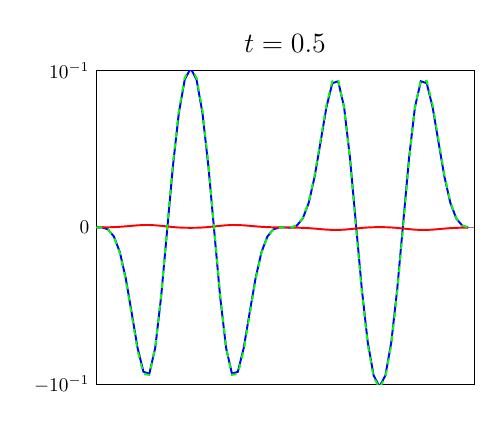
\begin{tikzpicture}[scale=0.7]

\begin{axis}[
    xtick = \empty,
    xmin = 0,
    xmax = 6.2832,
    ymin = -0.1,
    ymax = +0.1,
    ytick = {-0.1,0,0.1},
    yticklabels = {$-10^{-1}$,$0$,$10^{-1}$},
    scaled y ticks = false,
    scaled y ticks = false,
    title = {\Large $t = 0.5$},
  ]

\addplot[blue, line width=1pt] coordinates{
(0.0000e+00,6.0582e-12)
(9.8175e-02,6.4493e-05)
(1.9635e-01,-1.2452e-03)
(2.9452e-01,-5.7788e-03)
(3.9270e-01,-1.5693e-02)
(4.9087e-01,-3.2280e-02)
(5.8905e-01,-5.4213e-02)
(6.8722e-01,-7.6587e-02)
(7.8540e-01,-9.1961e-02)
(8.8357e-01,-9.3196e-02)
(9.8175e-01,-7.6651e-02)
(1.0799e+00,-4.4122e-02)
(1.1781e+00,-2.4484e-03)
(1.2763e+00,3.9226e-02)
(1.3744e+00,7.2989e-02)
(1.4726e+00,9.4253e-02)
(1.5708e+00,1.0142e-01)
(1.6690e+00,9.4253e-02)
(1.7671e+00,7.2989e-02)
(1.8653e+00,3.9226e-02)
(1.9635e+00,-2.4484e-03)
(2.0617e+00,-4.4122e-02)
(2.1598e+00,-7.6651e-02)
(2.2580e+00,-9.3196e-02)
(2.3562e+00,-9.1961e-02)
(2.4544e+00,-7.6587e-02)
(2.5525e+00,-5.4213e-02)
(2.6507e+00,-3.2280e-02)
(2.7489e+00,-1.5693e-02)
(2.8471e+00,-5.7788e-03)
(2.9452e+00,-1.2452e-03)
(3.0434e+00,6.4493e-05)
(3.1416e+00,6.6748e-12)
(3.2398e+00,-6.4493e-05)
(3.3379e+00,1.2452e-03)
(3.4361e+00,5.7788e-03)
(3.5343e+00,1.5693e-02)
(3.6325e+00,3.2280e-02)
(3.7306e+00,5.4213e-02)
(3.8288e+00,7.6587e-02)
(3.9270e+00,9.1961e-02)
(4.0252e+00,9.3196e-02)
(4.1233e+00,7.6651e-02)
(4.2215e+00,4.4122e-02)
(4.3197e+00,2.4484e-03)
(4.4179e+00,-3.9226e-02)
(4.5160e+00,-7.2989e-02)
(4.6142e+00,-9.4253e-02)
(4.7124e+00,-1.0142e-01)
(4.8106e+00,-9.4253e-02)
(4.9087e+00,-7.2989e-02)
(5.0069e+00,-3.9226e-02)
(5.1051e+00,2.4484e-03)
(5.2033e+00,4.4122e-02)
(5.3014e+00,7.6651e-02)
(5.3996e+00,9.3196e-02)
(5.4978e+00,9.1961e-02)
(5.5960e+00,7.6587e-02)
(5.6941e+00,5.4213e-02)
(5.7923e+00,3.2280e-02)
(5.8905e+00,1.5693e-02)
(5.9887e+00,5.7788e-03)
(6.0868e+00,1.2452e-03)
(6.1850e+00,-6.4493e-05)
};

\addplot[red, line width=1pt] coordinates{
(0.0000e+00,6.7339e-18)
(9.8175e-02,4.3333e-05)
(1.9635e-01,1.1058e-04)
(2.9452e-01,2.3031e-04)
(3.9270e-01,4.2984e-04)
(4.9087e-01,7.1540e-04)
(5.8905e-01,1.0514e-03)
(6.8722e-01,1.3614e-03)
(7.8540e-01,1.5567e-03)
(8.8357e-01,1.5722e-03)
(9.8175e-01,1.3903e-03)
(1.0799e+00,1.0511e-03)
(1.1781e+00,6.4307e-04)
(1.2763e+00,2.6721e-04)
(1.3744e+00,-7.6823e-06)
(1.4726e+00,-1.6322e-04)
(1.5708e+00,-2.1189e-04)
(1.6690e+00,-1.6322e-04)
(1.7671e+00,-7.6823e-06)
(1.8653e+00,2.6721e-04)
(1.9635e+00,6.4307e-04)
(2.0617e+00,1.0511e-03)
(2.1598e+00,1.3903e-03)
(2.2580e+00,1.5722e-03)
(2.3562e+00,1.5567e-03)
(2.4544e+00,1.3614e-03)
(2.5525e+00,1.0514e-03)
(2.6507e+00,7.1540e-04)
(2.7489e+00,4.2984e-04)
(2.8471e+00,2.3031e-04)
(2.9452e+00,1.1058e-04)
(3.0434e+00,4.3333e-05)
(3.1416e+00,-2.9592e-17)
(3.2398e+00,-4.3333e-05)
(3.3379e+00,-1.1058e-04)
(3.4361e+00,-2.3031e-04)
(3.5343e+00,-4.2984e-04)
(3.6325e+00,-7.1540e-04)
(3.7306e+00,-1.0514e-03)
(3.8288e+00,-1.3614e-03)
(3.9270e+00,-1.5567e-03)
(4.0252e+00,-1.5722e-03)
(4.1233e+00,-1.3903e-03)
(4.2215e+00,-1.0511e-03)
(4.3197e+00,-6.4307e-04)
(4.4179e+00,-2.6721e-04)
(4.5160e+00,7.6823e-06)
(4.6142e+00,1.6322e-04)
(4.7124e+00,2.1189e-04)
(4.8106e+00,1.6322e-04)
(4.9087e+00,7.6823e-06)
(5.0069e+00,-2.6721e-04)
(5.1051e+00,-6.4307e-04)
(5.2033e+00,-1.0511e-03)
(5.3014e+00,-1.3903e-03)
(5.3996e+00,-1.5722e-03)
(5.4978e+00,-1.5567e-03)
(5.5960e+00,-1.3614e-03)
(5.6941e+00,-1.0514e-03)
(5.7923e+00,-7.1540e-04)
(5.8905e+00,-4.2984e-04)
(5.9887e+00,-2.3031e-04)
(6.0868e+00,-1.1058e-04)
(6.1850e+00,-4.3333e-05)
};

\addplot[green, dashed, line width=1pt] coordinates{
(0.0000e+00,-3.9124e-12)
(9.8175e-02,2.0720e-05)
(1.9635e-01,-1.3715e-03)
(2.9452e-01,-6.0708e-03)
(3.9270e-01,-1.6268e-02)
(4.9087e-01,-3.3236e-02)
(5.8905e-01,-5.5539e-02)
(6.8722e-01,-7.8093e-02)
(7.8540e-01,-9.3289e-02)
(8.8357e-01,-9.3941e-02)
(9.8175e-01,-7.6532e-02)
(1.0799e+00,-4.3130e-02)
(1.1781e+00,-8.7651e-04)
(1.2763e+00,4.0917e-02)
(1.3744e+00,7.4420e-02)
(1.4726e+00,9.5324e-02)
(1.5708e+00,1.0233e-01)
(1.6690e+00,9.5324e-02)
(1.7671e+00,7.4420e-02)
(1.8653e+00,4.0917e-02)
(1.9635e+00,-8.7651e-04)
(2.0617e+00,-4.3130e-02)
(2.1598e+00,-7.6532e-02)
(2.2580e+00,-9.3941e-02)
(2.3562e+00,-9.3289e-02)
(2.4544e+00,-7.8093e-02)
(2.5525e+00,-5.5539e-02)
(2.6507e+00,-3.3236e-02)
(2.7489e+00,-1.6268e-02)
(2.8471e+00,-6.0708e-03)
(2.9452e+00,-1.3715e-03)
(3.0434e+00,2.0720e-05)
(3.1416e+00,5.6502e-13)
(3.2398e+00,-2.0720e-05)
(3.3379e+00,1.3715e-03)
(3.4361e+00,6.0708e-03)
(3.5343e+00,1.6268e-02)
(3.6325e+00,3.3236e-02)
(3.7306e+00,5.5539e-02)
(3.8288e+00,7.8093e-02)
(3.9270e+00,9.3289e-02)
(4.0252e+00,9.3941e-02)
(4.1233e+00,7.6532e-02)
(4.2215e+00,4.3130e-02)
(4.3197e+00,8.7651e-04)
(4.4179e+00,-4.0917e-02)
(4.5160e+00,-7.4420e-02)
(4.6142e+00,-9.5324e-02)
(4.7124e+00,-1.0233e-01)
(4.8106e+00,-9.5324e-02)
(4.9087e+00,-7.4420e-02)
(5.0069e+00,-4.0917e-02)
(5.1051e+00,8.7651e-04)
(5.2033e+00,4.3130e-02)
(5.3014e+00,7.6532e-02)
(5.3996e+00,9.3941e-02)
(5.4978e+00,9.3289e-02)
(5.5960e+00,7.8093e-02)
(5.6941e+00,5.5539e-02)
(5.7923e+00,3.3236e-02)
(5.8905e+00,1.6268e-02)
(5.9887e+00,6.0708e-03)
(6.0868e+00,1.3715e-03)
(6.1850e+00,-2.0720e-05)
};

\end{axis}



\end{tikzpicture}

%  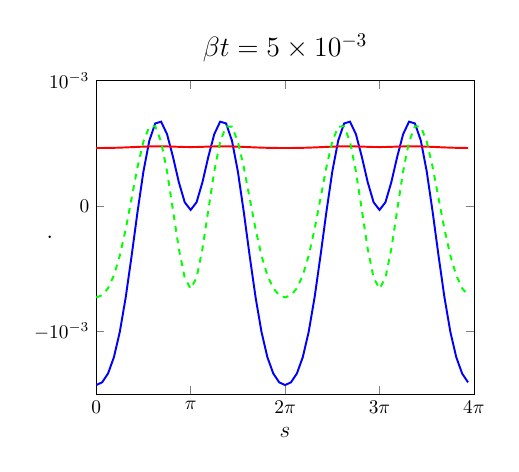
\begin{tikzpicture}[scale=0.7]

\begin{axis}[
    xmin = 0,
    xmax = 6.2832,
    xtick = {0,1.5708,3.1416,4.7124,6.2832},
    xticklabels = {$0$, $\pi$, $2\pi$, $3\pi$, $4\pi$},
    xlabel = {\large $s$},
    ymin = -0.0015,
    ymax = +0.001,
    ytick = {-0.001,0,0.001},
    yticklabels = {$-10^{-3}$,$0$,$10^{-3}$},
    ylabel = {\large $\uu \cdot \nn$},
    ylabel near ticks,
    ylabel shift = {-18pt},
    scaled y ticks = false,
    title = {\Large $\beta t = 5 \times 10^{-3}$},
  ]

\addplot[blue, line width=1pt] coordinates{
(0.0000e+00,-1.4252e-03)
(9.8175e-02,-1.4035e-03)
(1.9635e-01,-1.3334e-03)
(2.9452e-01,-1.2031e-03)
(3.9270e-01,-1.0011e-03)
(4.9087e-01,-7.2625e-04)
(5.8905e-01,-3.9562e-04)
(6.8722e-01,-4.5522e-05)
(7.8540e-01,2.7595e-04)
(8.8357e-01,5.2203e-04)
(9.8175e-01,6.5904e-04)
(1.0799e+00,6.7307e-04)
(1.1781e+00,5.7336e-04)
(1.2763e+00,3.9382e-04)
(1.3744e+00,1.9062e-04)
(1.4726e+00,3.0662e-05)
(1.5708e+00,-3.0007e-05)
(1.6690e+00,3.0662e-05)
(1.7671e+00,1.9062e-04)
(1.8653e+00,3.9382e-04)
(1.9635e+00,5.7336e-04)
(2.0617e+00,6.7307e-04)
(2.1598e+00,6.5904e-04)
(2.2580e+00,5.2203e-04)
(2.3562e+00,2.7595e-04)
(2.4544e+00,-4.5522e-05)
(2.5525e+00,-3.9562e-04)
(2.6507e+00,-7.2625e-04)
(2.7489e+00,-1.0011e-03)
(2.8471e+00,-1.2031e-03)
(2.9452e+00,-1.3334e-03)
(3.0434e+00,-1.4035e-03)
(3.1416e+00,-1.4252e-03)
(3.2398e+00,-1.4035e-03)
(3.3379e+00,-1.3334e-03)
(3.4361e+00,-1.2031e-03)
(3.5343e+00,-1.0011e-03)
(3.6325e+00,-7.2625e-04)
(3.7306e+00,-3.9562e-04)
(3.8288e+00,-4.5522e-05)
(3.9270e+00,2.7595e-04)
(4.0252e+00,5.2203e-04)
(4.1233e+00,6.5904e-04)
(4.2215e+00,6.7307e-04)
(4.3197e+00,5.7336e-04)
(4.4179e+00,3.9382e-04)
(4.5160e+00,1.9062e-04)
(4.6142e+00,3.0662e-05)
(4.7124e+00,-3.0007e-05)
(4.8106e+00,3.0662e-05)
(4.9087e+00,1.9062e-04)
(5.0069e+00,3.9382e-04)
(5.1051e+00,5.7336e-04)
(5.2033e+00,6.7307e-04)
(5.3014e+00,6.5904e-04)
(5.3996e+00,5.2203e-04)
(5.4978e+00,2.7595e-04)
(5.5960e+00,-4.5522e-05)
(5.6941e+00,-3.9562e-04)
(5.7923e+00,-7.2625e-04)
(5.8905e+00,-1.0011e-03)
(5.9887e+00,-1.2031e-03)
(6.0868e+00,-1.3334e-03)
(6.1850e+00,-1.4035e-03)
};

\addplot[red, line width=1pt] coordinates{
(0.0000e+00,4.6324e-04)
(9.8175e-02,4.6339e-04)
(1.9635e-01,4.6387e-04)
(2.9452e-01,4.6475e-04)
(3.9270e-01,4.6609e-04)
(4.9087e-01,4.6787e-04)
(5.8905e-01,4.6994e-04)
(6.8722e-01,4.7207e-04)
(7.8540e-01,4.7399e-04)
(8.8357e-01,4.7546e-04)
(9.8175e-01,4.7630e-04)
(1.0799e+00,4.7637e-04)
(1.1781e+00,4.7565e-04)
(1.2763e+00,4.7429e-04)
(1.3744e+00,4.7265e-04)
(1.4726e+00,4.7130e-04)
(1.5708e+00,4.7077e-04)
(1.6690e+00,4.7130e-04)
(1.7671e+00,4.7265e-04)
(1.8653e+00,4.7429e-04)
(1.9635e+00,4.7565e-04)
(2.0617e+00,4.7637e-04)
(2.1598e+00,4.7630e-04)
(2.2580e+00,4.7546e-04)
(2.3562e+00,4.7399e-04)
(2.4544e+00,4.7207e-04)
(2.5525e+00,4.6994e-04)
(2.6507e+00,4.6787e-04)
(2.7489e+00,4.6609e-04)
(2.8471e+00,4.6475e-04)
(2.9452e+00,4.6387e-04)
(3.0434e+00,4.6339e-04)
(3.1416e+00,4.6324e-04)
(3.2398e+00,4.6339e-04)
(3.3379e+00,4.6387e-04)
(3.4361e+00,4.6475e-04)
(3.5343e+00,4.6609e-04)
(3.6325e+00,4.6787e-04)
(3.7306e+00,4.6994e-04)
(3.8288e+00,4.7207e-04)
(3.9270e+00,4.7399e-04)
(4.0252e+00,4.7546e-04)
(4.1233e+00,4.7630e-04)
(4.2215e+00,4.7637e-04)
(4.3197e+00,4.7565e-04)
(4.4179e+00,4.7429e-04)
(4.5160e+00,4.7265e-04)
(4.6142e+00,4.7130e-04)
(4.7124e+00,4.7077e-04)
(4.8106e+00,4.7130e-04)
(4.9087e+00,4.7265e-04)
(5.0069e+00,4.7429e-04)
(5.1051e+00,4.7565e-04)
(5.2033e+00,4.7637e-04)
(5.3014e+00,4.7630e-04)
(5.3996e+00,4.7546e-04)
(5.4978e+00,4.7399e-04)
(5.5960e+00,4.7207e-04)
(5.6941e+00,4.6994e-04)
(5.7923e+00,4.6787e-04)
(5.8905e+00,4.6609e-04)
(5.9887e+00,4.6475e-04)
(6.0868e+00,4.6387e-04)
(6.1850e+00,4.6339e-04)
};

\addplot[green, dashed, line width=1pt] coordinates{
(0.0000e+00,-7.2674e-04)
(9.8175e-02,-7.0951e-04)
(1.9635e-01,-6.5403e-04)
(2.9452e-01,-5.5135e-04)
(3.9270e-01,-3.9376e-04)
(4.9087e-01,-1.8298e-04)
(5.8905e-01,6.3302e-05)
(6.8722e-01,3.1063e-04)
(7.8540e-01,5.1478e-04)
(8.8357e-01,6.3332e-04)
(9.8175e-01,6.3615e-04)
(1.0799e+00,5.1265e-04)
(1.1781e+00,2.7661e-04)
(1.2763e+00,-3.0169e-05)
(1.3744e+00,-3.3971e-04)
(1.4726e+00,-5.7126e-04)
(1.5708e+00,-6.5729e-04)
(1.6690e+00,-5.7126e-04)
(1.7671e+00,-3.3971e-04)
(1.8653e+00,-3.0169e-05)
(1.9635e+00,2.7661e-04)
(2.0617e+00,5.1265e-04)
(2.1598e+00,6.3615e-04)
(2.2580e+00,6.3332e-04)
(2.3562e+00,5.1478e-04)
(2.4544e+00,3.1063e-04)
(2.5525e+00,6.3302e-05)
(2.6507e+00,-1.8298e-04)
(2.7489e+00,-3.9376e-04)
(2.8471e+00,-5.5135e-04)
(2.9452e+00,-6.5403e-04)
(3.0434e+00,-7.0951e-04)
(3.1416e+00,-7.2674e-04)
(3.2398e+00,-7.0951e-04)
(3.3379e+00,-6.5403e-04)
(3.4361e+00,-5.5135e-04)
(3.5343e+00,-3.9376e-04)
(3.6325e+00,-1.8298e-04)
(3.7306e+00,6.3302e-05)
(3.8288e+00,3.1063e-04)
(3.9270e+00,5.1478e-04)
(4.0252e+00,6.3332e-04)
(4.1233e+00,6.3615e-04)
(4.2215e+00,5.1265e-04)
(4.3197e+00,2.7661e-04)
(4.4179e+00,-3.0169e-05)
(4.5160e+00,-3.3971e-04)
(4.6142e+00,-5.7126e-04)
(4.7124e+00,-6.5729e-04)
(4.8106e+00,-5.7126e-04)
(4.9087e+00,-3.3971e-04)
(5.0069e+00,-3.0169e-05)
(5.1051e+00,2.7661e-04)
(5.2033e+00,5.1265e-04)
(5.3014e+00,6.3615e-04)
(5.3996e+00,6.3332e-04)
(5.4978e+00,5.1478e-04)
(5.5960e+00,3.1063e-04)
(5.6941e+00,6.3302e-05)
(5.7923e+00,-1.8298e-04)
(5.8905e+00,-3.9376e-04)
(5.9887e+00,-5.5135e-04)
(6.0868e+00,-6.5403e-04)
(6.1850e+00,-7.0951e-04)
};

\end{axis}


\end{tikzpicture}

%  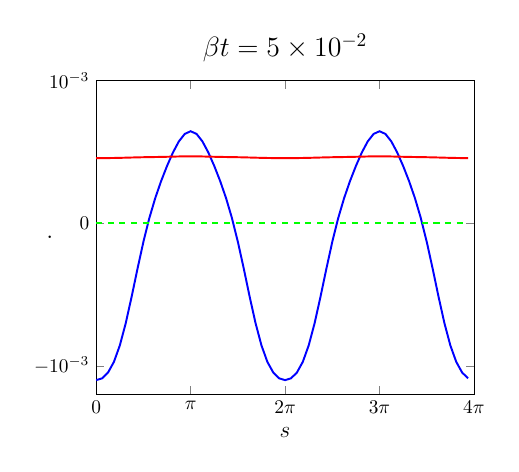
\begin{tikzpicture}[scale=0.7]


\begin{axis}[
    xmin = 0,
    xmax = 6.2832,
    xtick = {0,1.5708,3.1416,4.7124,6.2832},
    xticklabels = {$0$, $\pi$, $2\pi$, $3\pi$, $4\pi$},
    xlabel = {\large $s$},
    ymin = -0.0012,
    ymax = +0.001,
    ytick = {-0.001,0,0.001},
    yticklabels = {$-10^{-3}$,$0$,$10^{-3}$},
    ylabel = {\large $\uu \cdot \nn$},
    ylabel near ticks,
    ylabel shift = {-18pt},
    scaled y ticks = false,
    title = {\Large $\beta t = 5 \times 10^{-2}$},
  ]

\addplot[blue, line width=1pt] coordinates{
(0.0000e+00,-1.0996e-03)
(9.8175e-02,-1.0870e-03)
(1.9635e-01,-1.0466e-03)
(2.9452e-01,-9.7170e-04)
(3.9270e-01,-8.5638e-04)
(4.9087e-01,-7.0082e-04)
(5.8905e-01,-5.1507e-04)
(6.8722e-01,-3.1782e-04)
(7.8540e-01,-1.2954e-04)
(8.8357e-01,3.6091e-05)
(9.8175e-01,1.7622e-04)
(1.0799e+00,2.9597e-04)
(1.1781e+00,4.0183e-04)
(1.2763e+00,4.9586e-04)
(1.3744e+00,5.7370e-04)
(1.4726e+00,6.2639e-04)
(1.5708e+00,6.4517e-04)
(1.6690e+00,6.2639e-04)
(1.7671e+00,5.7370e-04)
(1.8653e+00,4.9586e-04)
(1.9635e+00,4.0183e-04)
(2.0617e+00,2.9597e-04)
(2.1598e+00,1.7622e-04)
(2.2580e+00,3.6091e-05)
(2.3562e+00,-1.2954e-04)
(2.4544e+00,-3.1782e-04)
(2.5525e+00,-5.1507e-04)
(2.6507e+00,-7.0082e-04)
(2.7489e+00,-8.5638e-04)
(2.8471e+00,-9.7170e-04)
(2.9452e+00,-1.0466e-03)
(3.0434e+00,-1.0870e-03)
(3.1416e+00,-1.0996e-03)
(3.2398e+00,-1.0870e-03)
(3.3379e+00,-1.0466e-03)
(3.4361e+00,-9.7170e-04)
(3.5343e+00,-8.5638e-04)
(3.6325e+00,-7.0082e-04)
(3.7306e+00,-5.1507e-04)
(3.8288e+00,-3.1782e-04)
(3.9270e+00,-1.2954e-04)
(4.0252e+00,3.6091e-05)
(4.1233e+00,1.7622e-04)
(4.2215e+00,2.9597e-04)
(4.3197e+00,4.0183e-04)
(4.4179e+00,4.9586e-04)
(4.5160e+00,5.7370e-04)
(4.6142e+00,6.2639e-04)
(4.7124e+00,6.4517e-04)
(4.8106e+00,6.2639e-04)
(4.9087e+00,5.7370e-04)
(5.0069e+00,4.9586e-04)
(5.1051e+00,4.0183e-04)
(5.2033e+00,2.9597e-04)
(5.3014e+00,1.7622e-04)
(5.3996e+00,3.6091e-05)
(5.4978e+00,-1.2954e-04)
(5.5960e+00,-3.1782e-04)
(5.6941e+00,-5.1507e-04)
(5.7923e+00,-7.0082e-04)
(5.8905e+00,-8.5638e-04)
(5.9887e+00,-9.7170e-04)
(6.0868e+00,-1.0466e-03)
(6.1850e+00,-1.0870e-03)
};

\addplot[red, line width=1pt] coordinates{
(0.0000e+00,4.5667e-04)
(9.8175e-02,4.5678e-04)
(1.9635e-01,4.5711e-04)
(2.9452e-01,4.5772e-04)
(3.9270e-01,4.5862e-04)
(4.9087e-01,4.5975e-04)
(5.8905e-01,4.6097e-04)
(6.8722e-01,4.6210e-04)
(7.8540e-01,4.6302e-04)
(8.8357e-01,4.6376e-04)
(9.8175e-01,4.6444e-04)
(1.0799e+00,4.6521e-04)
(1.1781e+00,4.6616e-04)
(1.2763e+00,4.6723e-04)
(1.3744e+00,4.6829e-04)
(1.4726e+00,4.6908e-04)
(1.5708e+00,4.6938e-04)
(1.6690e+00,4.6908e-04)
(1.7671e+00,4.6829e-04)
(1.8653e+00,4.6723e-04)
(1.9635e+00,4.6616e-04)
(2.0617e+00,4.6521e-04)
(2.1598e+00,4.6444e-04)
(2.2580e+00,4.6376e-04)
(2.3562e+00,4.6302e-04)
(2.4544e+00,4.6210e-04)
(2.5525e+00,4.6097e-04)
(2.6507e+00,4.5975e-04)
(2.7489e+00,4.5862e-04)
(2.8471e+00,4.5772e-04)
(2.9452e+00,4.5711e-04)
(3.0434e+00,4.5678e-04)
(3.1416e+00,4.5667e-04)
(3.2398e+00,4.5678e-04)
(3.3379e+00,4.5711e-04)
(3.4361e+00,4.5772e-04)
(3.5343e+00,4.5862e-04)
(3.6325e+00,4.5975e-04)
(3.7306e+00,4.6097e-04)
(3.8288e+00,4.6210e-04)
(3.9270e+00,4.6302e-04)
(4.0252e+00,4.6376e-04)
(4.1233e+00,4.6444e-04)
(4.2215e+00,4.6521e-04)
(4.3197e+00,4.6616e-04)
(4.4179e+00,4.6723e-04)
(4.5160e+00,4.6829e-04)
(4.6142e+00,4.6908e-04)
(4.7124e+00,4.6938e-04)
(4.8106e+00,4.6908e-04)
(4.9087e+00,4.6829e-04)
(5.0069e+00,4.6723e-04)
(5.1051e+00,4.6616e-04)
(5.2033e+00,4.6521e-04)
(5.3014e+00,4.6444e-04)
(5.3996e+00,4.6376e-04)
(5.4978e+00,4.6302e-04)
(5.5960e+00,4.6210e-04)
(5.6941e+00,4.6097e-04)
(5.7923e+00,4.5975e-04)
(5.8905e+00,4.5862e-04)
(5.9887e+00,4.5772e-04)
(6.0868e+00,4.5711e-04)
(6.1850e+00,4.5678e-04)
};

\addplot[green, dashed, line width=1pt] coordinates{
(0.0000e+00,-2.3701e-12)
(9.8175e-02,-5.1013e-12)
(1.9635e-01,-2.1890e-12)
(2.9452e-01,-3.5219e-12)
(3.9270e-01,-1.5410e-12)
(4.9087e-01,-1.8243e-12)
(5.8905e-01,-4.6256e-13)
(6.8722e-01,8.3140e-13)
(7.8540e-01,1.0570e-12)
(8.8357e-01,2.3248e-12)
(9.8175e-01,2.1470e-12)
(1.0799e+00,3.2332e-12)
(1.1781e+00,2.3841e-12)
(1.2763e+00,3.6752e-12)
(1.3744e+00,2.7500e-12)
(1.4726e+00,3.8911e-12)
(1.5708e+00,3.0465e-12)
(1.6690e+00,3.7839e-12)
(1.7671e+00,2.9670e-12)
(1.8653e+00,3.3832e-12)
(1.9635e+00,2.5833e-12)
(2.0617e+00,3.1272e-12)
(2.1598e+00,1.9943e-12)
(2.2580e+00,2.8072e-12)
(2.3562e+00,4.5835e-13)
(2.4544e+00,1.8049e-12)
(2.5525e+00,-1.7784e-12)
(2.6507e+00,4.5430e-13)
(2.7489e+00,-4.4271e-12)
(2.8471e+00,-1.2356e-12)
(2.9452e+00,-4.6053e-12)
(3.0434e+00,-2.1283e-12)
(3.1416e+00,-5.5059e-12)
(3.2398e+00,-3.2576e-12)
(3.3379e+00,-2.5917e-12)
(3.4361e+00,-3.6846e-12)
(3.5343e+00,-1.2203e-12)
(3.6325e+00,-2.5257e-12)
(3.7306e+00,4.3051e-13)
(3.8288e+00,-1.0295e-13)
(3.9270e+00,2.0464e-12)
(4.0252e+00,1.3831e-12)
(4.1233e+00,3.1439e-12)
(4.2215e+00,2.1068e-12)
(4.3197e+00,3.5191e-12)
(4.4179e+00,2.5897e-12)
(4.5160e+00,3.8035e-12)
(4.6142e+00,2.9385e-12)
(4.7124e+00,3.9496e-12)
(4.8106e+00,2.9646e-12)
(4.9087e+00,3.7350e-12)
(5.0069e+00,2.6137e-12)
(5.1051e+00,3.3981e-12)
(5.2033e+00,2.3594e-12)
(5.3014e+00,2.9610e-12)
(5.3996e+00,1.6281e-12)
(5.4978e+00,1.7719e-12)
(5.5960e+00,1.6160e-13)
(5.6941e+00,-2.2854e-13)
(5.7923e+00,-1.1349e-12)
(5.8905e+00,-2.8796e-12)
(5.9887e+00,-2.9905e-12)
(6.0868e+00,-2.1672e-12)
(6.1850e+00,-5.0508e-12)
};

\end{axis}

\end{tikzpicture}

%  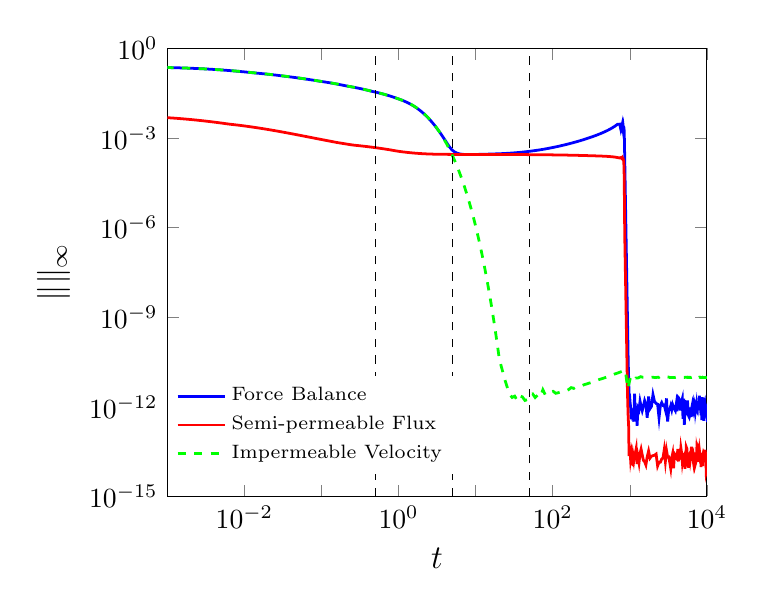
\begin{tikzpicture}[scale=1]

  \begin{axis}[
    name = maxPlot,
    xmin = 1e-3,
    xmax = 10000,
    ymin = 1e-15,
    ymax = 1e0,
    xmode = log,
    ymode = log,
    xminorticks = false,
    yminorticks = false,
    xtick = {1e-3,1e-2,1e-1,1e0,1e1,1e2,1e3,1e4},
    xticklabels = {,$10^{-2}$,,$10^0$,,$10^2$,,$10^4$},
    xlabel = {\large $t$},
    ylabel = {\large $\|\uu\|_\infty$},
    ylabel near ticks,
    legend entries = {Force Balance,
    Semi-permeable Flux,Impermeable Velocity},
    legend cell align=left,
    legend style={draw=none,font=\scriptsize},
    legend style={at={(0.0,0.05)},anchor=south west}
  ]

\addplot[blue, line width=1pt] coordinates{
(0.0000e+00,2.5143e-01)
(6.4149e-05,2.4906e-01)
(1.2188e-04,2.4693e-01)
(1.8424e-04,2.4478e-01)
(2.5158e-04,2.4254e-01)
(3.2431e-04,2.4022e-01)
(4.0286e-04,2.3783e-01)
(4.8769e-04,2.3537e-01)
(5.7930e-04,2.3284e-01)
(6.7825e-04,2.3024e-01)
(7.8511e-04,2.2773e-01)
(9.0052e-04,2.2619e-01)
(1.0252e-03,2.2455e-01)
(1.1598e-03,2.2283e-01)
(1.3052e-03,2.2100e-01)
(1.4622e-03,2.1908e-01)
(1.6318e-03,2.1706e-01)
(1.8149e-03,2.1494e-01)
(2.0127e-03,2.1273e-01)
(2.2263e-03,2.1043e-01)
(2.4570e-03,2.0804e-01)
(2.7062e-03,2.0557e-01)
(2.9753e-03,2.0301e-01)
(3.2659e-03,2.0037e-01)
(3.5798e-03,1.9766e-01)
(3.9188e-03,1.9487e-01)
(4.2849e-03,1.9201e-01)
(4.6803e-03,1.8909e-01)
(5.1073e-03,1.8610e-01)
(5.5685e-03,1.8306e-01)
(6.0666e-03,1.7997e-01)
(6.6045e-03,1.7683e-01)
(7.1855e-03,1.7365e-01)
(7.8129e-03,1.7043e-01)
(8.4905e-03,1.6718e-01)
(9.2224e-03,1.6390e-01)
(9.9991e-03,1.6066e-01)
(1.0827e-02,1.5743e-01)
(1.1702e-02,1.5426e-01)
(1.2641e-02,1.5108e-01)
(1.3621e-02,1.4800e-01)
(1.4679e-02,1.4543e-01)
(1.5779e-02,1.4296e-01)
(1.6968e-02,1.4043e-01)
(1.8208e-02,1.3794e-01)
(1.9547e-02,1.3539e-01)
(2.0933e-02,1.3290e-01)
(2.2430e-02,1.3035e-01)
(2.3996e-02,1.2782e-01)
(2.5687e-02,1.2523e-01)
(2.7422e-02,1.2273e-01)
(2.9295e-02,1.2015e-01)
(3.1276e-02,1.1758e-01)
(3.3376e-02,1.1510e-01)
(3.5593e-02,1.1281e-01)
(3.7949e-02,1.1053e-01)
(4.0425e-02,1.0827e-01)
(4.3074e-02,1.0599e-01)
(4.5826e-02,1.0377e-01)
(4.8797e-02,1.0149e-01)
(5.1865e-02,9.9283e-02)
(5.5178e-02,9.7024e-02)
(5.8630e-02,9.4806e-02)
(6.2358e-02,9.2538e-02)
(6.6187e-02,9.0543e-02)
(7.0322e-02,8.8527e-02)
(7.4666e-02,8.6516e-02)
(7.9318e-02,8.4459e-02)
(8.4141e-02,8.2434e-02)
(8.9350e-02,8.0349e-02)
(9.4748e-02,7.8401e-02)
(1.0058e-01,7.6656e-02)
(1.0663e-01,7.4942e-02)
(1.1316e-01,7.3178e-02)
(1.1994e-01,7.1447e-02)
(1.2725e-01,6.9669e-02)
(1.3486e-01,6.7918e-02)
(1.4308e-01,6.6121e-02)
(1.5159e-01,6.4360e-02)
(1.6079e-01,6.2557e-02)
(1.7039e-01,6.0778e-02)
(1.8076e-01,5.8961e-02)
(1.9148e-01,5.7215e-02)
(2.0304e-01,5.5535e-02)
(2.1521e-01,5.3906e-02)
(2.2829e-01,5.2503e-02)
(2.4187e-01,5.1119e-02)
(2.5654e-01,4.9696e-02)
(2.7191e-01,4.8285e-02)
(2.8850e-01,4.6839e-02)
(3.0579e-01,4.5415e-02)
(3.2446e-01,4.3960e-02)
(3.4425e-01,4.2507e-02)
(3.6555e-01,4.1032e-02)
(3.8802e-01,3.9571e-02)
(4.1229e-01,3.8090e-02)
(4.3823e-01,3.6663e-02)
(4.6618e-01,3.5256e-02)
(4.9600e-01,3.4003e-02)
(5.2821e-01,3.2752e-02)
(5.6259e-01,3.1488e-02)
(5.9972e-01,3.0196e-02)
(6.3901e-01,2.8902e-02)
(6.8145e-01,2.7582e-02)
(7.2600e-01,2.6334e-02)
(7.7412e-01,2.5064e-02)
(8.2397e-01,2.3816e-02)
(8.7782e-01,2.2537e-02)
(9.3363e-01,2.1296e-02)
(9.9391e-01,2.0088e-02)
(1.0560e+00,1.8988e-02)
(1.1231e+00,1.7874e-02)
(1.1935e+00,1.6761e-02)
(1.2696e+00,1.5602e-02)
(1.3493e+00,1.4457e-02)
(1.4353e+00,1.3282e-02)
(1.5282e+00,1.2101e-02)
(1.6286e+00,1.0921e-02)
(1.7370e+00,9.7569e-03)
(1.8540e+00,8.6206e-03)
(1.9805e+00,7.5269e-03)
(2.1170e+00,6.4886e-03)
(2.2645e+00,5.5180e-03)
(2.4237e+00,4.6252e-03)
(2.5957e+00,3.8178e-03)
(2.7815e+00,3.1018e-03)
(2.9821e+00,2.4840e-03)
(3.1988e+00,1.9590e-03)
(3.4328e+00,1.5197e-03)
(3.6855e+00,1.1615e-03)
(3.9584e+00,8.7926e-04)
(4.2532e+00,6.5945e-04)
(4.5716e+00,4.9988e-04)
(4.9154e+00,3.9480e-04)
(5.2868e+00,3.4142e-04)
(5.6878e+00,3.0992e-04)
(6.1209e+00,2.9209e-04)
(6.5887e+00,2.8332e-04)
(7.0939e+00,2.7818e-04)
(7.6395e+00,2.7687e-04)
(8.2288e+00,2.7653e-04)
(8.8652e+00,2.7680e-04)
(9.5525e+00,2.7748e-04)
(1.0295e+01,2.7843e-04)
(1.1096e+01,2.7956e-04)
(1.1962e+01,2.8085e-04)
(1.2897e+01,2.8227e-04)
(1.3907e+01,2.8381e-04)
(1.4998e+01,2.8549e-04)
(1.6176e+01,2.8731e-04)
(1.7448e+01,2.8927e-04)
(1.8822e+01,2.9140e-04)
(2.0306e+01,2.9371e-04)
(2.1908e+01,2.9620e-04)
(2.3639e+01,2.9906e-04)
(2.5509e+01,3.0232e-04)
(2.7527e+01,3.0615e-04)
(2.9708e+01,3.1030e-04)
(3.2062e+01,3.1485e-04)
(3.4605e+01,3.2004e-04)
(3.7352e+01,3.2577e-04)
(4.0318e+01,3.3238e-04)
(4.3522e+01,3.3966e-04)
(4.6982e+01,3.4754e-04)
(5.0718e+01,3.5606e-04)
(5.4754e+01,3.6529e-04)
(5.9112e+01,3.7527e-04)
(6.3819e+01,3.8609e-04)
(6.8903e+01,3.9780e-04)
(7.4393e+01,4.1106e-04)
(8.0323e+01,4.2566e-04)
(8.6727e+01,4.4148e-04)
(9.3643e+01,4.5860e-04)
(1.0111e+02,4.7716e-04)
(1.0918e+02,4.9728e-04)
(1.1789e+02,5.1910e-04)
(1.2730e+02,5.4279e-04)
(1.3746e+02,5.6851e-04)
(1.4844e+02,5.9648e-04)
(1.6029e+02,6.2690e-04)
(1.7309e+02,6.6004e-04)
(1.8692e+02,6.9619e-04)
(2.0185e+02,7.3567e-04)
(2.1798e+02,7.7888e-04)
(2.3539e+02,8.2627e-04)
(2.5420e+02,8.7860e-04)
(2.7452e+02,9.3646e-04)
(2.9646e+02,1.0004e-03)
(3.2015e+02,1.0713e-03)
(3.4574e+02,1.1504e-03)
(3.7338e+02,1.2392e-03)
(4.0323e+02,1.3396e-03)
(4.3546e+02,1.4544e-03)
(4.7028e+02,1.5874e-03)
(5.0788e+02,1.7443e-03)
(5.4849e+02,1.9321e-03)
(5.9234e+02,2.1625e-03)
(6.3971e+02,2.4532e-03)
(6.9087e+02,2.8309e-03)
(7.3860e+02,2.8717e-03)
(7.6471e+02,1.8870e-03)
(7.8821e+02,2.5831e-03)
(7.9978e+02,1.5132e-03)
(8.1019e+02,2.1951e-03)
(8.1786e+02,1.8397e-03)
(8.2476e+02,2.1848e-03)
(8.2894e+02,1.9639e-03)
(8.3270e+02,2.1935e-03)
(8.3676e+02,2.1955e-03)
(8.4008e+02,2.0963e-03)
(8.4307e+02,1.8359e-03)
(8.4630e+02,1.3692e-03)
(8.4979e+02,8.5321e-04)
(8.5355e+02,4.6151e-04)
(8.5762e+02,2.2880e-04)
(8.6201e+02,1.0623e-04)
(8.6676e+02,4.6574e-05)
(8.7188e+02,1.9205e-05)
(8.7741e+02,7.4416e-06)
(8.8339e+02,2.6891e-06)
(8.8984e+02,9.0581e-07)
(8.9681e+02,2.8105e-07)
(9.0434e+02,8.0677e-08)
(9.1247e+02,2.0930e-08)
(9.2125e+02,5.0195e-09)
(9.3074e+02,1.0411e-09)
(9.4098e+02,2.1553e-10)
(9.5204e+02,3.3127e-11)
(9.6399e+02,1.0173e-11)
(9.7689e+02,2.6156e-12)
(9.9082e+02,2.5647e-12)
(1.0059e+03,1.4604e-12)
(1.0221e+03,1.0297e-12)
(1.0397e+03,3.8532e-13)
(1.0586e+03,8.7966e-13)
(1.0791e+03,5.6448e-13)
(1.1012e+03,6.7332e-13)
(1.1251e+03,3.1864e-13)
(1.1509e+03,2.7655e-12)
(1.1787e+03,4.3047e-13)
(1.2088e+03,9.2874e-13)
(1.2413e+03,2.3389e-13)
(1.2764e+03,9.1925e-13)
(1.3143e+03,7.9248e-13)
(1.3552e+03,1.5394e-12)
(1.3994e+03,1.0368e-12)
(1.4472e+03,7.4452e-13)
(1.4987e+03,1.0463e-12)
(1.5544e+03,1.6068e-12)
(1.6145e+03,1.2030e-12)
(1.6795e+03,4.3113e-13)
(1.7496e+03,2.2264e-12)
(1.8254e+03,8.6291e-13)
(1.9072e+03,1.0332e-12)
(1.9955e+03,2.5592e-12)
(2.0910e+03,1.4926e-12)
(2.1910e+03,1.3019e-12)
(2.2910e+03,1.2244e-12)
(2.3910e+03,4.2932e-13)
(2.4910e+03,1.1290e-12)
(2.5910e+03,1.3855e-12)
(2.6910e+03,1.1209e-12)
(2.7910e+03,1.1519e-12)
(2.8910e+03,7.9919e-13)
(2.9910e+03,1.9182e-12)
(3.0910e+03,3.2355e-13)
(3.1910e+03,7.8306e-13)
(3.2910e+03,8.0543e-13)
(3.3910e+03,1.0720e-12)
(3.4910e+03,7.9869e-13)
(3.5910e+03,1.1848e-12)
(3.6910e+03,9.7610e-13)
(3.7910e+03,8.4733e-13)
(3.8910e+03,7.4753e-13)
(3.9910e+03,1.1734e-12)
(4.0910e+03,7.0933e-13)
(4.1910e+03,2.1420e-12)
(4.2910e+03,2.0005e-12)
(4.3910e+03,1.7126e-12)
(4.4910e+03,8.2398e-13)
(4.5910e+03,8.2245e-13)
(4.6910e+03,1.5379e-12)
(4.7910e+03,1.8778e-12)
(4.8910e+03,3.9299e-13)
(4.9910e+03,1.8851e-12)
(5.0910e+03,2.5074e-13)
(5.1910e+03,9.8207e-13)
(5.2910e+03,9.0016e-13)
(5.3910e+03,1.6474e-12)
(5.4910e+03,5.2017e-13)
(5.5910e+03,1.6420e-12)
(5.6910e+03,7.9097e-13)
(5.7910e+03,4.9046e-13)
(5.8910e+03,4.4748e-13)
(5.9910e+03,5.4278e-13)
(6.0910e+03,9.5033e-13)
(6.1910e+03,4.5112e-13)
(6.2910e+03,8.8500e-13)
(6.3910e+03,1.0037e-12)
(6.4910e+03,1.2334e-12)
(6.5910e+03,9.5577e-13)
(6.6910e+03,1.4078e-12)
(6.7910e+03,4.8365e-13)
(6.8910e+03,1.3804e-12)
(6.9910e+03,1.2211e-12)
(7.0910e+03,7.2179e-13)
(7.1910e+03,9.3724e-13)
(7.2910e+03,1.1978e-12)
(7.3910e+03,7.6460e-13)
(7.4910e+03,7.1138e-13)
(7.5910e+03,1.4478e-12)
(7.6910e+03,9.7540e-13)
(7.7910e+03,9.4444e-13)
(7.8910e+03,7.7455e-13)
(7.9910e+03,2.3758e-12)
(8.0910e+03,1.3559e-12)
(8.1910e+03,8.2851e-13)
(8.2910e+03,7.7395e-13)
(8.3910e+03,5.2508e-13)
(8.4910e+03,1.5877e-12)
(8.5910e+03,3.6241e-13)
(8.6910e+03,2.0898e-12)
(8.7910e+03,1.1283e-12)
(8.8910e+03,5.7107e-13)
(8.9910e+03,8.8000e-13)
(9.0910e+03,3.4033e-13)
(9.1910e+03,1.9988e-12)
(9.2910e+03,1.2492e-12)
(9.3910e+03,1.3974e-12)
(9.4910e+03,1.1016e-12)
(9.5910e+03,8.3162e-13)
(9.6910e+03,9.6957e-13)
(9.7910e+03,9.9004e-13)
(9.8910e+03,1.1992e-12)
(9.9910e+03,7.0748e-13)
(1.0091e+04,8.0575e-13)
(1.0191e+04,4.0864e-13)
(1.0291e+04,3.1129e-13)
(1.0391e+04,5.2996e-13)
(1.0491e+04,2.2481e-12)
(1.0591e+04,7.9016e-13)
(1.0691e+04,9.1354e-13)
(1.0791e+04,4.7389e-13)
(1.0891e+04,6.1893e-13)
(1.0991e+04,1.8346e-12)
(1.1091e+04,1.5432e-12)
(1.1191e+04,9.1388e-13)
(1.1291e+04,8.0937e-13)
(1.1391e+04,1.5291e-12)
(1.1491e+04,8.5536e-13)
(1.1591e+04,1.9577e-12)
(1.1691e+04,8.2352e-13)
(1.1791e+04,1.0942e-12)
(1.1891e+04,9.8388e-13)
(1.1991e+04,1.6554e-12)
(1.2091e+04,1.3927e-12)
(1.2191e+04,9.2175e-13)
(1.2291e+04,1.0800e-12)
(1.2391e+04,6.8912e-13)
(1.2491e+04,6.7045e-13)
(1.2591e+04,1.3170e-12)
(1.2691e+04,1.0000e-12)
(1.2791e+04,6.0368e-13)
(1.2891e+04,4.6551e-13)
(1.2991e+04,4.2708e-13)
(1.3091e+04,7.9265e-13)
(1.3191e+04,1.0978e-12)
(1.3291e+04,1.0257e-12)
(1.3391e+04,5.0769e-13)
(1.3491e+04,1.4083e-12)
(1.3591e+04,8.9094e-13)
(1.3691e+04,1.4698e-12)
(1.3791e+04,9.7415e-13)
(1.3891e+04,8.7689e-13)
(1.3991e+04,6.3129e-13)
(1.4091e+04,7.5509e-13)
(1.4191e+04,1.8049e-12)
(1.4291e+04,5.0680e-13)
(1.4391e+04,1.2294e-12)
(1.4491e+04,1.5597e-12)
(1.4591e+04,5.4681e-13)
(1.4691e+04,9.8953e-13)
(1.4791e+04,1.1934e-12)
(1.4891e+04,1.7594e-12)
(1.4991e+04,1.6216e-12)
(1.5091e+04,7.2236e-13)
(1.5191e+04,1.9573e-12)
(1.5291e+04,4.4939e-13)
(1.5391e+04,1.4691e-12)
(1.5491e+04,1.2943e-12)
(1.5591e+04,2.4329e-12)
(1.5691e+04,1.6416e-12)
(1.5791e+04,1.2694e-12)
(1.5891e+04,8.1613e-13)
(1.5991e+04,6.8194e-13)
(1.6091e+04,1.5994e-12)
(1.6191e+04,3.7993e-13)
(1.6291e+04,1.3779e-12)
(1.6391e+04,1.2776e-12)
(1.6491e+04,5.6385e-13)
(1.6591e+04,1.6089e-12)
(1.6691e+04,2.0244e-12)
(1.6791e+04,2.0989e-12)
(1.6891e+04,1.7240e-12)
(1.6991e+04,1.4830e-12)
(1.7091e+04,1.5747e-12)
(1.7191e+04,1.5543e-12)
(1.7291e+04,7.0006e-13)
(1.7391e+04,1.3472e-12)
(1.7491e+04,3.4862e-13)
(1.7591e+04,1.2367e-12)
(1.7691e+04,7.0192e-13)
(1.7791e+04,6.6082e-13)
(1.7891e+04,4.8511e-13)
(1.7991e+04,1.3491e-12)
(1.8091e+04,6.3469e-13)
(1.8191e+04,1.9423e-12)
(1.8291e+04,1.2199e-12)
(1.8391e+04,8.7569e-13)
(1.8491e+04,8.7707e-13)
(1.8591e+04,1.4653e-12)
(1.8691e+04,1.7261e-12)
(1.8791e+04,1.2364e-12)
(1.8891e+04,7.5528e-13)
(1.8991e+04,4.3179e-13)
(1.9091e+04,6.1800e-13)
(1.9191e+04,1.5140e-12)
(1.9291e+04,9.4249e-13)
(1.9391e+04,9.7265e-13)
(1.9491e+04,1.2219e-12)
(1.9591e+04,5.4964e-13)
(1.9691e+04,1.7148e-12)
(1.9791e+04,9.5472e-13)
(1.9891e+04,8.7837e-13)
(1.9991e+04,3.7547e-13)
(2.0000e+04,4.7031e-13)
};

\addplot[red, line width=1pt] coordinates{
(0.0000e+00,5.6693e-03)
(6.4149e-05,5.6070e-03)
(1.2188e-04,5.5480e-03)
(1.8424e-04,5.4839e-03)
(2.5158e-04,5.4139e-03)
(3.2431e-04,5.3388e-03)
(4.0286e-04,5.2588e-03)
(4.8769e-04,5.1745e-03)
(5.7930e-04,5.0862e-03)
(6.7825e-04,4.9945e-03)
(7.8511e-04,4.8999e-03)
(9.0052e-04,4.8029e-03)
(1.0252e-03,4.7041e-03)
(1.1598e-03,4.6038e-03)
(1.3052e-03,4.5025e-03)
(1.4622e-03,4.4006e-03)
(1.6318e-03,4.2983e-03)
(1.8149e-03,4.1958e-03)
(2.0127e-03,4.0934e-03)
(2.2263e-03,3.9913e-03)
(2.4570e-03,3.8896e-03)
(2.7062e-03,3.7884e-03)
(2.9753e-03,3.6879e-03)
(3.2659e-03,3.5882e-03)
(3.5798e-03,3.4893e-03)
(3.9188e-03,3.3914e-03)
(4.2849e-03,3.2947e-03)
(4.6803e-03,3.1991e-03)
(5.1073e-03,3.1048e-03)
(5.5685e-03,3.0120e-03)
(6.0666e-03,2.9206e-03)
(6.6045e-03,2.8397e-03)
(7.1855e-03,2.7728e-03)
(7.8129e-03,2.7048e-03)
(8.4905e-03,2.6360e-03)
(9.2224e-03,2.5666e-03)
(9.9991e-03,2.4980e-03)
(1.0827e-02,2.4299e-03)
(1.1702e-02,2.3632e-03)
(1.2641e-02,2.2969e-03)
(1.3621e-02,2.2328e-03)
(1.4679e-02,2.1688e-03)
(1.5779e-02,2.1072e-03)
(1.6968e-02,2.0459e-03)
(1.8208e-02,1.9868e-03)
(1.9547e-02,1.9280e-03)
(2.0933e-02,1.8720e-03)
(2.2430e-02,1.8163e-03)
(2.3996e-02,1.7626e-03)
(2.5687e-02,1.7094e-03)
(2.7422e-02,1.6591e-03)
(2.9295e-02,1.6092e-03)
(3.1276e-02,1.5608e-03)
(3.3376e-02,1.5136e-03)
(3.5593e-02,1.4679e-03)
(3.7949e-02,1.4234e-03)
(4.0425e-02,1.3804e-03)
(4.3074e-02,1.3383e-03)
(4.5826e-02,1.2981e-03)
(4.8797e-02,1.2584e-03)
(5.1865e-02,1.2207e-03)
(5.5178e-02,1.1835e-03)
(5.8630e-02,1.1479e-03)
(6.2358e-02,1.1129e-03)
(6.6187e-02,1.0797e-03)
(7.0322e-02,1.0471e-03)
(7.4666e-02,1.0156e-03)
(7.9318e-02,9.8477e-04)
(8.4141e-02,9.5547e-04)
(8.9350e-02,9.2771e-04)
(9.4748e-02,9.0119e-04)
(1.0058e-01,8.7493e-04)
(1.0663e-01,8.4973e-04)
(1.1316e-01,8.2472e-04)
(1.1994e-01,8.0175e-04)
(1.2725e-01,7.7887e-04)
(1.3486e-01,7.5669e-04)
(1.4308e-01,7.3449e-04)
(1.5159e-01,7.1299e-04)
(1.6079e-01,6.9400e-04)
(1.7039e-01,6.7759e-04)
(1.8076e-01,6.6117e-04)
(1.9148e-01,6.4538e-04)
(2.0304e-01,6.2948e-04)
(2.1521e-01,6.1393e-04)
(2.2829e-01,5.9921e-04)
(2.4187e-01,5.8578e-04)
(2.5654e-01,5.7434e-04)
(2.7191e-01,5.6389e-04)
(2.8850e-01,5.5493e-04)
(3.0579e-01,5.4624e-04)
(3.2446e-01,5.3727e-04)
(3.4425e-01,5.2835e-04)
(3.6555e-01,5.1914e-04)
(3.8802e-01,5.0994e-04)
(4.1229e-01,5.0036e-04)
(4.3823e-01,4.9059e-04)
(4.6618e-01,4.8044e-04)
(4.9600e-01,4.7006e-04)
(5.2821e-01,4.5973e-04)
(5.6259e-01,4.4973e-04)
(5.9972e-01,4.3934e-04)
(6.3901e-01,4.2889e-04)
(6.8145e-01,4.1805e-04)
(7.2600e-01,4.0731e-04)
(7.7412e-01,3.9623e-04)
(8.2397e-01,3.8552e-04)
(8.7782e-01,3.7451e-04)
(9.3363e-01,3.6409e-04)
(9.9391e-01,3.5501e-04)
(1.0560e+00,3.4721e-04)
(1.1231e+00,3.3996e-04)
(1.1935e+00,3.3369e-04)
(1.2696e+00,3.2756e-04)
(1.3493e+00,3.2206e-04)
(1.4353e+00,3.1687e-04)
(1.5282e+00,3.1206e-04)
(1.6286e+00,3.0756e-04)
(1.7370e+00,3.0343e-04)
(1.8540e+00,2.9968e-04)
(1.9805e+00,2.9630e-04)
(2.1170e+00,2.9331e-04)
(2.2645e+00,2.9068e-04)
(2.4237e+00,2.8840e-04)
(2.5957e+00,2.8645e-04)
(2.7815e+00,2.8481e-04)
(2.9821e+00,2.8345e-04)
(3.1988e+00,2.8233e-04)
(3.4328e+00,2.8143e-04)
(3.6855e+00,2.8072e-04)
(3.9584e+00,2.8016e-04)
(4.2532e+00,2.7973e-04)
(4.5716e+00,2.7940e-04)
(4.9154e+00,2.7916e-04)
(5.2868e+00,2.7897e-04)
(5.6878e+00,2.7883e-04)
(6.1209e+00,2.7872e-04)
(6.5887e+00,2.7863e-04)
(7.0939e+00,2.7855e-04)
(7.6395e+00,2.7847e-04)
(8.2288e+00,2.7840e-04)
(8.8652e+00,2.7833e-04)
(9.5525e+00,2.7825e-04)
(1.0295e+01,2.7817e-04)
(1.1096e+01,2.7808e-04)
(1.1962e+01,2.7799e-04)
(1.2897e+01,2.7788e-04)
(1.3907e+01,2.7777e-04)
(1.4998e+01,2.7765e-04)
(1.6176e+01,2.7753e-04)
(1.7448e+01,2.7739e-04)
(1.8822e+01,2.7724e-04)
(2.0306e+01,2.7708e-04)
(2.1908e+01,2.7690e-04)
(2.3639e+01,2.7671e-04)
(2.5509e+01,2.7651e-04)
(2.7527e+01,2.7629e-04)
(2.9708e+01,2.7605e-04)
(3.2062e+01,2.7580e-04)
(3.4605e+01,2.7552e-04)
(3.7352e+01,2.7523e-04)
(4.0318e+01,2.7490e-04)
(4.3522e+01,2.7456e-04)
(4.6982e+01,2.7419e-04)
(5.0718e+01,2.7378e-04)
(5.4754e+01,2.7335e-04)
(5.9112e+01,2.7288e-04)
(6.3819e+01,2.7238e-04)
(6.8903e+01,2.7183e-04)
(7.4393e+01,2.7124e-04)
(8.0323e+01,2.7065e-04)
(8.6727e+01,2.7007e-04)
(9.3643e+01,2.6944e-04)
(1.0111e+02,2.6876e-04)
(1.0918e+02,2.6803e-04)
(1.1789e+02,2.6724e-04)
(1.2730e+02,2.6639e-04)
(1.3746e+02,2.6548e-04)
(1.4844e+02,2.6449e-04)
(1.6029e+02,2.6342e-04)
(1.7309e+02,2.6227e-04)
(1.8692e+02,2.6103e-04)
(2.0185e+02,2.5986e-04)
(2.1798e+02,2.5863e-04)
(2.3539e+02,2.5730e-04)
(2.5420e+02,2.5586e-04)
(2.7452e+02,2.5437e-04)
(2.9646e+02,2.5292e-04)
(3.2015e+02,2.5134e-04)
(3.4574e+02,2.4980e-04)
(3.7338e+02,2.4820e-04)
(4.0323e+02,2.4643e-04)
(4.3546e+02,2.4443e-04)
(4.7028e+02,2.4214e-04)
(5.0788e+02,2.3947e-04)
(5.4849e+02,2.3624e-04)
(5.9234e+02,2.3218e-04)
(6.3971e+02,2.2674e-04)
(6.9087e+02,2.1876e-04)
(7.3860e+02,2.1165e-04)
(7.6471e+02,2.1850e-04)
(7.8821e+02,2.0199e-04)
(7.9978e+02,2.1512e-04)
(8.1019e+02,1.9615e-04)
(8.1786e+02,1.9725e-04)
(8.2476e+02,1.7795e-04)
(8.2894e+02,1.7558e-04)
(8.3270e+02,1.5295e-04)
(8.3676e+02,1.2683e-04)
(8.4008e+02,9.5715e-05)
(8.4307e+02,6.1539e-05)
(8.4630e+02,2.9768e-05)
(8.4979e+02,1.0317e-05)
(8.5355e+02,2.7336e-06)
(8.5762e+02,6.9224e-07)
(8.6201e+02,3.0044e-07)
(8.6676e+02,1.3603e-07)
(8.7188e+02,5.7548e-08)
(8.7741e+02,2.2651e-08)
(8.8339e+02,8.2446e-09)
(8.8984e+02,2.8171e-09)
(8.9681e+02,8.7232e-10)
(9.0434e+02,2.5644e-10)
(9.1247e+02,6.5383e-11)
(9.2125e+02,1.6783e-11)
(9.3074e+02,3.2506e-12)
(9.4098e+02,1.1296e-12)
(9.5204e+02,4.3169e-13)
(9.6399e+02,2.3733e-13)
(9.7689e+02,2.2621e-14)
(9.9082e+02,4.3649e-14)
(1.0059e+03,3.4117e-14)
(1.0221e+03,1.7449e-14)
(1.0397e+03,2.3844e-14)
(1.0586e+03,1.2719e-14)
(1.0791e+03,1.2123e-14)
(1.1012e+03,2.3179e-14)
(1.1251e+03,1.6207e-14)
(1.1509e+03,2.5628e-14)
(1.1787e+03,2.8429e-14)
(1.2088e+03,3.9962e-14)
(1.2413e+03,1.2196e-14)
(1.2764e+03,2.0626e-14)
(1.3143e+03,1.3292e-14)
(1.3552e+03,2.7086e-14)
(1.3994e+03,3.8263e-14)
(1.4472e+03,2.4673e-14)
(1.4987e+03,1.6260e-14)
(1.5544e+03,1.4749e-14)
(1.6145e+03,1.1371e-14)
(1.6795e+03,2.1419e-14)
(1.7496e+03,3.2947e-14)
(1.8254e+03,1.9222e-14)
(1.9072e+03,2.2400e-14)
(1.9955e+03,2.3172e-14)
(2.0910e+03,2.3993e-14)
(2.1910e+03,2.6299e-14)
(2.2910e+03,1.0545e-14)
(2.3910e+03,1.4095e-14)
(2.4910e+03,1.4118e-14)
(2.5910e+03,1.7952e-14)
(2.6910e+03,1.9555e-14)
(2.7910e+03,3.6036e-14)
(2.8910e+03,1.4932e-14)
(2.9910e+03,3.4162e-14)
(3.0910e+03,2.0982e-14)
(3.1910e+03,2.1237e-14)
(3.2910e+03,1.4081e-14)
(3.3910e+03,8.7783e-15)
(3.4910e+03,1.9536e-14)
(3.5910e+03,2.7275e-14)
(3.6910e+03,8.7754e-15)
(3.7910e+03,2.6815e-14)
(3.8910e+03,2.4278e-14)
(3.9910e+03,1.8711e-14)
(4.0910e+03,1.7574e-14)
(4.1910e+03,3.8939e-14)
(4.2910e+03,2.1952e-14)
(4.3910e+03,1.8438e-14)
(4.4910e+03,2.0446e-14)
(4.5910e+03,4.2310e-14)
(4.6910e+03,2.9090e-14)
(4.7910e+03,1.4671e-14)
(4.8910e+03,2.1928e-14)
(4.9910e+03,2.3796e-14)
(5.0910e+03,1.5050e-14)
(5.1910e+03,8.4461e-15)
(5.2910e+03,1.4975e-14)
(5.3910e+03,4.5208e-14)
(5.4910e+03,3.9769e-14)
(5.5910e+03,1.0303e-14)
(5.6910e+03,1.5348e-14)
(5.7910e+03,9.1048e-15)
(5.8910e+03,2.4236e-14)
(5.9910e+03,2.6767e-14)
(6.0910e+03,1.7249e-14)
(6.1910e+03,2.3393e-14)
(6.2910e+03,4.6190e-14)
(6.3910e+03,2.4691e-14)
(6.4910e+03,2.4260e-14)
(6.5910e+03,2.7087e-14)
(6.6910e+03,1.3509e-14)
(6.7910e+03,1.0599e-14)
(6.8910e+03,1.3049e-14)
(6.9910e+03,2.9886e-14)
(7.0910e+03,1.2369e-14)
(7.1910e+03,1.4245e-14)
(7.2910e+03,1.6823e-14)
(7.3910e+03,3.9814e-14)
(7.4910e+03,3.2972e-14)
(7.5910e+03,2.5795e-14)
(7.6910e+03,1.4391e-14)
(7.7910e+03,2.9495e-14)
(7.8910e+03,2.5102e-14)
(7.9910e+03,3.4773e-14)
(8.0910e+03,2.6366e-14)
(8.1910e+03,2.5085e-14)
(8.2910e+03,2.4418e-14)
(8.3910e+03,9.6396e-15)
(8.4910e+03,2.8596e-14)
(8.5910e+03,2.3453e-14)
(8.6910e+03,2.3874e-14)
(8.7910e+03,1.0467e-14)
(8.8910e+03,2.5197e-14)
(8.9910e+03,2.9020e-14)
(9.0910e+03,2.6943e-14)
(9.1910e+03,2.1377e-14)
(9.2910e+03,1.3795e-14)
(9.3910e+03,3.0234e-14)
(9.4910e+03,3.6269e-14)
(9.5910e+03,1.7869e-14)
(9.6910e+03,1.7195e-14)
(9.7910e+03,6.6374e-15)
(9.8910e+03,7.4312e-15)
(9.9910e+03,3.1134e-14)
(1.0091e+04,1.2721e-14)
(1.0191e+04,2.3357e-14)
(1.0291e+04,2.4906e-14)
(1.0391e+04,1.9568e-14)
(1.0491e+04,2.3754e-14)
(1.0591e+04,3.1157e-14)
(1.0691e+04,2.5085e-14)
(1.0791e+04,2.9293e-14)
(1.0891e+04,2.2021e-14)
(1.0991e+04,2.2934e-14)
(1.1091e+04,1.5633e-14)
(1.1191e+04,2.1718e-14)
(1.1291e+04,4.8615e-14)
(1.1391e+04,2.5722e-14)
(1.1491e+04,1.2631e-14)
(1.1591e+04,3.6677e-14)
(1.1691e+04,1.7100e-14)
(1.1791e+04,3.8447e-14)
(1.1891e+04,4.4168e-14)
(1.1991e+04,3.8039e-14)
(1.2091e+04,1.3166e-14)
(1.2191e+04,1.0820e-14)
(1.2291e+04,1.5829e-14)
(1.2391e+04,1.7789e-14)
(1.2491e+04,7.2545e-15)
(1.2591e+04,1.8568e-14)
(1.2691e+04,3.0936e-14)
(1.2791e+04,2.0484e-14)
(1.2891e+04,1.6596e-14)
(1.2991e+04,2.9214e-14)
(1.3091e+04,2.0248e-14)
(1.3191e+04,3.6711e-14)
(1.3291e+04,2.9857e-14)
(1.3391e+04,9.6160e-15)
(1.3491e+04,2.0237e-14)
(1.3591e+04,2.2302e-14)
(1.3691e+04,2.3002e-14)
(1.3791e+04,2.7511e-14)
(1.3891e+04,1.6357e-14)
(1.3991e+04,1.9212e-14)
(1.4091e+04,2.5781e-14)
(1.4191e+04,3.2396e-14)
(1.4291e+04,1.5631e-14)
(1.4391e+04,1.2267e-14)
(1.4491e+04,1.9854e-14)
(1.4591e+04,1.7628e-14)
(1.4691e+04,3.4073e-14)
(1.4791e+04,4.2443e-14)
(1.4891e+04,3.0432e-14)
(1.4991e+04,4.2351e-14)
(1.5091e+04,4.1907e-14)
(1.5191e+04,2.3215e-14)
(1.5291e+04,2.3100e-14)
(1.5391e+04,1.8164e-14)
(1.5491e+04,2.9011e-14)
(1.5591e+04,2.1870e-14)
(1.5691e+04,2.2520e-14)
(1.5791e+04,1.4747e-14)
(1.5891e+04,2.4073e-14)
(1.5991e+04,3.7654e-14)
(1.6091e+04,2.4416e-14)
(1.6191e+04,1.1497e-14)
(1.6291e+04,1.7328e-14)
(1.6391e+04,4.3015e-14)
(1.6491e+04,1.8581e-14)
(1.6591e+04,1.5256e-14)
(1.6691e+04,2.5442e-14)
(1.6791e+04,1.7565e-14)
(1.6891e+04,1.6557e-14)
(1.6991e+04,2.0475e-14)
(1.7091e+04,1.5720e-14)
(1.7191e+04,8.4512e-15)
(1.7291e+04,1.4006e-14)
(1.7391e+04,1.8519e-14)
(1.7491e+04,7.7379e-15)
(1.7591e+04,2.8026e-14)
(1.7691e+04,2.6360e-14)
(1.7791e+04,1.4545e-14)
(1.7891e+04,2.5924e-14)
(1.7991e+04,1.9612e-14)
(1.8091e+04,1.2754e-14)
(1.8191e+04,8.6501e-15)
(1.8291e+04,2.3384e-14)
(1.8391e+04,2.9081e-14)
(1.8491e+04,2.0677e-14)
(1.8591e+04,1.1112e-14)
(1.8691e+04,2.8848e-14)
(1.8791e+04,1.9517e-14)
(1.8891e+04,1.4772e-14)
(1.8991e+04,2.1345e-14)
(1.9091e+04,2.9260e-14)
(1.9191e+04,1.3769e-14)
(1.9291e+04,1.1431e-14)
(1.9391e+04,3.7128e-14)
(1.9491e+04,2.4117e-14)
(1.9591e+04,1.2209e-14)
(1.9691e+04,3.2980e-14)
(1.9791e+04,1.7004e-14)
(1.9891e+04,7.7523e-15)
(1.9991e+04,2.1033e-14)
(2.0000e+04,3.4849e-14)
};

\addplot[green, dashed, line width=1pt] coordinates{
(0.0000e+00,2.5098e-01)
(7.9049e-05,2.4823e-01)
(1.5019e-04,2.4578e-01)
(2.2703e-04,2.4332e-01)
(3.1001e-04,2.4076e-01)
(3.9963e-04,2.3814e-01)
(4.9642e-04,2.3544e-01)
(6.0096e-04,2.3267e-01)
(7.1386e-04,2.2984e-01)
(8.3578e-04,2.2695e-01)
(9.6747e-04,2.2505e-01)
(1.1097e-03,2.2328e-01)
(1.2633e-03,2.2141e-01)
(1.4292e-03,2.1945e-01)
(1.6083e-03,2.1738e-01)
(1.8018e-03,2.1521e-01)
(2.0108e-03,2.1294e-01)
(2.2364e-03,2.1058e-01)
(2.4802e-03,2.0813e-01)
(2.7434e-03,2.0559e-01)
(3.0277e-03,2.0297e-01)
(3.3348e-03,2.0026e-01)
(3.6664e-03,1.9748e-01)
(4.0245e-03,1.9462e-01)
(4.4113e-03,1.9170e-01)
(4.8290e-03,1.8871e-01)
(5.2801e-03,1.8566e-01)
(5.7674e-03,1.8256e-01)
(6.2936e-03,1.7940e-01)
(6.8619e-03,1.7620e-01)
(7.4756e-03,1.7296e-01)
(8.1385e-03,1.6969e-01)
(8.8544e-03,1.6639e-01)
(9.6276e-03,1.6306e-01)
(1.0429e-02,1.5984e-01)
(1.1295e-02,1.5660e-01)
(1.2214e-02,1.5340e-01)
(1.3192e-02,1.5022e-01)
(1.4225e-02,1.4709e-01)
(1.5331e-02,1.4437e-01)
(1.6488e-02,1.4187e-01)
(1.7738e-02,1.3932e-01)
(1.9029e-02,1.3683e-01)
(2.0424e-02,1.3428e-01)
(2.1890e-02,1.3174e-01)
(2.3464e-02,1.2917e-01)
(2.5097e-02,1.2664e-01)
(2.6859e-02,1.2406e-01)
(2.8694e-02,1.2151e-01)
(3.0676e-02,1.1890e-01)
(3.2723e-02,1.1635e-01)
(3.4934e-02,1.1395e-01)
(3.7243e-02,1.1167e-01)
(3.9737e-02,1.0936e-01)
(4.2293e-02,1.0713e-01)
(4.5055e-02,1.0486e-01)
(4.7967e-02,1.0260e-01)
(5.1066e-02,1.0034e-01)
(5.4316e-02,9.8096e-02)
(5.7805e-02,9.5823e-02)
(6.1408e-02,9.3609e-02)
(6.5298e-02,9.1347e-02)
(6.9355e-02,8.9278e-02)
(7.3737e-02,8.7235e-02)
(7.8235e-02,8.5243e-02)
(8.3094e-02,8.3187e-02)
(8.8208e-02,8.1133e-02)
(9.3669e-02,7.9046e-02)
(9.9365e-02,7.7232e-02)
(1.0552e-01,7.5475e-02)
(1.1184e-01,7.3764e-02)
(1.1868e-01,7.2004e-02)
(1.2587e-01,7.0250e-02)
(1.3357e-01,6.8467e-02)
(1.4158e-01,6.6710e-02)
(1.5024e-01,6.4908e-02)
(1.5921e-01,6.3143e-02)
(1.6889e-01,6.1337e-02)
(1.7902e-01,5.9555e-02)
(1.8995e-01,5.7736e-02)
(2.0124e-01,5.5975e-02)
(2.1344e-01,5.4293e-02)
(2.2629e-01,5.2798e-02)
(2.4007e-01,5.1392e-02)
(2.5445e-01,5.0000e-02)
(2.6998e-01,4.8570e-02)
(2.8618e-01,4.7158e-02)
(3.0368e-01,4.5712e-02)
(3.2208e-01,4.4277e-02)
(3.4196e-01,4.2812e-02)
(3.6284e-01,4.1364e-02)
(3.8539e-01,3.9891e-02)
(4.0944e-01,3.8418e-02)
(4.3536e-01,3.6930e-02)
(4.6292e-01,3.5511e-02)
(4.9269e-01,3.4157e-02)
(5.2462e-01,3.2921e-02)
(5.5898e-01,3.1659e-02)
(5.9572e-01,3.0383e-02)
(6.3524e-01,2.9084e-02)
(6.7718e-01,2.7782e-02)
(7.2235e-01,2.6465e-02)
(7.6958e-01,2.5224e-02)
(8.2059e-01,2.3952e-02)
(8.7343e-01,2.2703e-02)
(9.3049e-01,2.1424e-02)
(9.8957e-01,2.0216e-02)
(1.0534e+00,1.9058e-02)
(1.1195e+00,1.7981e-02)
(1.1909e+00,1.6853e-02)
(1.2660e+00,1.5728e-02)
(1.3470e+00,1.4563e-02)
(1.4332e+00,1.3401e-02)
(1.5262e+00,1.2221e-02)
(1.6266e+00,1.1043e-02)
(1.7351e+00,9.8758e-03)
(1.8523e+00,8.7355e-03)
(1.9788e+00,7.6349e-03)
(2.1155e+00,6.5880e-03)
(2.2631e+00,5.6074e-03)
(2.4225e+00,4.7028e-03)
(2.5946e+00,3.8825e-03)
(2.7805e+00,3.1517e-03)
(2.9813e+00,2.5129e-03)
(3.1982e+00,1.9657e-03)
(3.4324e+00,1.5067e-03)
(3.6854e+00,1.1301e-03)
(3.9585e+00,8.2839e-04)
(4.2536e+00,5.9253e-04)
(4.5722e+00,4.1293e-04)
(4.9163e+00,2.7991e-04)
(5.2880e+00,1.8423e-04)
(5.6894e+00,1.1754e-04)
(6.1229e+00,7.2550e-05)
(6.5911e+00,4.3221e-05)
(7.0967e+00,2.4795e-05)
(7.6428e+00,1.3666e-05)
(8.2326e+00,7.2190e-06)
(8.8696e+00,3.6443e-06)
(9.5575e+00,1.7531e-06)
(1.0300e+01,8.0117e-07)
(1.1103e+01,3.4671e-07)
(1.1969e+01,1.4160e-07)
(1.2905e+01,5.4375e-08)
(1.3916e+01,1.9557e-08)
(1.5008e+01,6.5601e-09)
(1.6187e+01,2.0439e-09)
(1.7460e+01,5.8862e-10)
(1.8835e+01,1.5597e-10)
(2.0320e+01,3.8143e-11)
(2.1924e+01,1.8633e-11)
(2.3657e+01,8.7763e-12)
(2.5528e+01,4.7407e-12)
(2.7548e+01,2.6355e-12)
(2.9730e+01,2.0559e-12)
(3.2087e+01,2.2771e-12)
(3.4632e+01,1.6226e-12)
(3.7381e+01,2.3248e-12)
(4.0350e+01,2.1554e-12)
(4.3557e+01,1.6344e-12)
(4.7020e+01,1.7455e-12)
(5.0759e+01,2.5639e-12)
(5.4799e+01,2.7186e-12)
(5.9161e+01,2.0402e-12)
(6.3872e+01,2.4824e-12)
(6.8960e+01,2.1381e-12)
(7.4455e+01,3.7182e-12)
(8.0390e+01,2.4513e-12)
(8.6800e+01,2.8169e-12)
(9.3722e+01,3.0758e-12)
(1.0120e+02,3.3028e-12)
(1.0927e+02,2.8365e-12)
(1.1799e+02,2.9590e-12)
(1.2741e+02,3.1587e-12)
(1.3758e+02,3.2125e-12)
(1.4857e+02,3.4191e-12)
(1.6043e+02,3.7651e-12)
(1.7324e+02,4.3911e-12)
(1.8708e+02,4.1412e-12)
(2.0203e+02,4.6815e-12)
(2.1817e+02,4.8861e-12)
(2.3560e+02,5.0417e-12)
(2.5442e+02,5.4703e-12)
(2.7476e+02,5.8246e-12)
(2.9671e+02,6.1999e-12)
(3.2043e+02,6.5984e-12)
(3.4604e+02,7.1861e-12)
(3.7370e+02,7.6200e-12)
(4.0358e+02,8.2710e-12)
(4.3584e+02,8.7611e-12)
(4.7069e+02,9.3601e-12)
(5.0832e+02,1.0088e-11)
(5.4897e+02,1.1181e-11)
(5.9286e+02,1.1686e-11)
(6.4027e+02,1.2610e-11)
(6.9147e+02,1.3457e-11)
(7.4677e+02,1.4485e-11)
(8.0649e+02,1.5671e-11)
(8.7098e+02,1.6867e-11)
(9.4064e+02,4.0698e-12)
(1.0159e+03,9.3937e-12)
(1.0971e+03,7.3120e-12)
(1.1849e+03,9.1161e-12)
(1.2796e+03,9.2852e-12)
(1.3796e+03,1.0204e-11)
(1.4796e+03,9.7565e-12)
(1.5796e+03,9.7371e-12)
(1.6796e+03,9.6417e-12)
(1.7796e+03,9.9750e-12)
(1.8796e+03,9.6146e-12)
(1.9796e+03,9.8207e-12)
(2.0796e+03,9.5693e-12)
(2.1796e+03,9.5532e-12)
(2.2796e+03,9.7414e-12)
(2.3796e+03,9.6510e-12)
(2.4796e+03,1.0366e-11)
(2.5796e+03,9.7363e-12)
(2.6796e+03,9.7004e-12)
(2.7796e+03,9.5434e-12)
(2.8796e+03,9.5641e-12)
(2.9796e+03,9.6679e-12)
(3.0796e+03,9.9416e-12)
(3.1796e+03,9.8994e-12)
(3.2796e+03,9.6315e-12)
(3.3796e+03,9.5663e-12)
(3.4796e+03,9.5860e-12)
(3.5796e+03,9.6156e-12)
(3.6796e+03,9.5202e-12)
(3.7796e+03,9.6394e-12)
(3.8796e+03,9.6259e-12)
(3.9796e+03,9.8050e-12)
(4.0796e+03,9.7616e-12)
(4.1796e+03,9.5942e-12)
(4.2796e+03,9.8353e-12)
(4.3796e+03,9.7715e-12)
(4.4796e+03,9.5369e-12)
(4.5796e+03,9.5675e-12)
(4.6796e+03,9.5829e-12)
(4.7796e+03,9.7260e-12)
(4.8796e+03,9.6628e-12)
(4.9796e+03,9.5908e-12)
(5.0796e+03,9.5705e-12)
(5.1796e+03,9.7122e-12)
(5.2796e+03,9.8086e-12)
(5.3796e+03,9.7163e-12)
(5.4796e+03,9.6569e-12)
(5.5796e+03,9.7917e-12)
(5.6796e+03,9.5615e-12)
(5.7796e+03,9.6810e-12)
(5.8796e+03,9.5562e-12)
(5.9796e+03,9.7869e-12)
(6.0796e+03,9.6950e-12)
(6.1796e+03,9.5704e-12)
(6.2796e+03,9.5730e-12)
(6.3796e+03,9.7137e-12)
(6.4796e+03,9.5541e-12)
(6.5796e+03,9.5534e-12)
(6.6796e+03,9.5564e-12)
(6.7796e+03,9.5413e-12)
(6.8796e+03,9.5431e-12)
(6.9796e+03,9.8308e-12)
(7.0796e+03,9.8837e-12)
(7.1796e+03,1.0448e-11)
(7.2796e+03,9.7986e-12)
(7.3796e+03,9.6981e-12)
(7.4796e+03,9.5304e-12)
(7.5796e+03,9.5552e-12)
(7.6796e+03,9.6131e-12)
(7.7796e+03,9.5730e-12)
(7.8796e+03,9.7423e-12)
(7.9796e+03,9.7285e-12)
(8.0796e+03,9.8376e-12)
(8.1796e+03,9.5912e-12)
(8.2796e+03,9.5550e-12)
(8.3796e+03,9.5594e-12)
(8.4796e+03,9.5739e-12)
(8.5796e+03,9.6410e-12)
(8.6796e+03,9.6251e-12)
(8.7796e+03,9.7819e-12)
(8.8796e+03,9.6298e-12)
(8.9796e+03,9.5849e-12)
(9.0796e+03,9.5444e-12)
(9.1796e+03,9.5641e-12)
(9.2796e+03,9.5916e-12)
(9.3796e+03,9.6237e-12)
(9.4796e+03,9.5538e-12)
(9.5796e+03,9.6400e-12)
(9.6796e+03,9.5797e-12)
(9.7796e+03,9.5703e-12)
(9.8796e+03,9.6225e-12)
(9.9796e+03,9.6496e-12)
(1.0080e+04,9.8844e-12)
(1.0180e+04,9.5379e-12)
(1.0280e+04,9.5550e-12)
(1.0380e+04,9.5713e-12)
(1.0480e+04,9.6333e-12)
(1.0580e+04,9.5724e-12)
(1.0680e+04,9.5701e-12)
(1.0780e+04,9.5285e-12)
(1.0880e+04,9.8690e-12)
(1.0980e+04,9.8649e-12)
(1.1080e+04,1.0032e-11)
(1.1180e+04,1.0056e-11)
(1.1280e+04,9.5417e-12)
(1.1380e+04,9.7058e-12)
(1.1480e+04,9.5483e-12)
(1.1580e+04,9.6052e-12)
(1.1680e+04,9.5557e-12)
(1.1780e+04,9.6531e-12)
(1.1880e+04,9.5540e-12)
(1.1980e+04,9.6653e-12)
(1.2080e+04,9.5918e-12)
(1.2180e+04,9.6198e-12)
(1.2280e+04,9.5496e-12)
(1.2380e+04,9.7144e-12)
(1.2480e+04,9.5753e-12)
(1.2580e+04,9.6531e-12)
(1.2680e+04,9.5840e-12)
(1.2780e+04,9.5498e-12)
(1.2880e+04,9.6000e-12)
(1.2980e+04,9.5583e-12)
(1.3080e+04,9.5210e-12)
(1.3180e+04,9.5396e-12)
(1.3280e+04,9.5434e-12)
(1.3380e+04,9.9768e-12)
(1.3480e+04,9.7135e-12)
(1.3580e+04,9.5574e-12)
(1.3680e+04,9.6302e-12)
(1.3780e+04,9.5745e-12)
(1.3880e+04,9.6905e-12)
(1.3980e+04,9.5725e-12)
(1.4080e+04,9.6554e-12)
(1.4180e+04,9.5887e-12)
(1.4280e+04,9.6255e-12)
(1.4380e+04,9.7616e-12)
(1.4480e+04,9.8713e-12)
(1.4580e+04,9.5477e-12)
(1.4680e+04,9.7461e-12)
(1.4780e+04,9.7021e-12)
(1.4880e+04,9.5554e-12)
(1.4980e+04,9.6217e-12)
(1.5080e+04,9.5405e-12)
(1.5180e+04,9.6090e-12)
(1.5280e+04,9.5911e-12)
(1.5380e+04,9.5638e-12)
(1.5480e+04,9.7680e-12)
(1.5580e+04,9.5617e-12)
(1.5680e+04,9.5644e-12)
(1.5780e+04,9.6752e-12)
(1.5880e+04,9.7885e-12)
(1.5980e+04,9.5624e-12)
(1.6080e+04,9.6919e-12)
(1.6180e+04,9.6169e-12)
(1.6280e+04,9.6907e-12)
(1.6380e+04,9.5615e-12)
(1.6480e+04,9.8517e-12)
(1.6580e+04,9.6741e-12)
(1.6680e+04,9.7514e-12)
(1.6780e+04,9.7950e-12)
(1.6880e+04,9.7215e-12)
(1.6980e+04,9.9650e-12)
(1.7080e+04,9.7248e-12)
(1.7180e+04,9.6043e-12)
(1.7280e+04,9.5804e-12)
(1.7380e+04,9.5615e-12)
(1.7480e+04,9.7110e-12)
(1.7580e+04,9.5265e-12)
(1.7680e+04,9.5805e-12)
(1.7780e+04,1.0197e-11)
(1.7880e+04,9.7436e-12)
(1.7980e+04,9.6708e-12)
(1.8080e+04,9.5530e-12)
(1.8180e+04,9.5492e-12)
(1.8280e+04,9.6187e-12)
(1.8380e+04,9.6512e-12)
(1.8480e+04,9.6485e-12)
(1.8580e+04,9.6259e-12)
(1.8680e+04,9.5648e-12)
(1.8780e+04,9.5386e-12)
(1.8880e+04,9.5722e-12)
(1.8980e+04,9.6344e-12)
(1.9080e+04,9.5776e-12)
(1.9180e+04,9.7229e-12)
(1.9280e+04,9.7991e-12)
(1.9380e+04,9.5130e-12)
(1.9480e+04,9.6170e-12)
(1.9580e+04,9.6116e-12)
(1.9680e+04,9.5596e-12)
(1.9780e+04,9.5719e-12)
(1.9880e+04,9.5480e-12)
(1.9980e+04,9.6638e-12)
(2.0000e+04,6.3391e-12)
};

\addplot[black, dashed, line width=0.4pt] coordinates{
  (0.5,1e-15)
  (0.5,1)
};

\addplot[black, dashed, line width=0.4pt] coordinates{
  (5,1e-15)
  (5,1)
};

\addplot[black, dashed, line width=0.4pt] coordinates{
  (50,1e-15)
  (50,1)
};

\end{axis}


\end{tikzpicture}

  \includegraphics[width=0.48\linewidth]{figures/ellipseVelocity1.pdf}
  \includegraphics[width=0.48\linewidth]{figures/ellipseVelocity2.pdf}
  \includegraphics[width=0.48\linewidth]{figures/ellipseVelocity3.pdf}
  \includegraphics[width=0.48\linewidth]{figures/ellipseVelocityNorms.pdf}
  \caption{\label{fig:vesVelocity} The velocity contributions due to
  force balance (blue) and permeability (red). The green dashed line is
  the velocity of an impermeable vesicle with the same initial shape as
  the semi-permeable vesicle. The bottom right plot is the max norm of
  each contributor to the vesicle velocities. The three black lines
  correspond to the times reported in the other three plots.}
\end{figure}

\todo[inline]{left off here}
We next investigate the interplay between the tension, flux, and
curvature of a semi-permeable vesicle. We let $\beta = 1$ and initialize
the vesicle with regions of both positive and negative curvature. The
vesicle tension, $\Lambda$, and the flux, $\ff \cdot \nn$, are plotted
in Figure~\ref{fig:starTensionFlux}. The vesicle undergoes three general
behaviors: (i) For $t \in (0,1.6 \times 10^{-2})$, the vesicle has a net
negative flux resulting in a loss of area; (ii) For $t \in (1.6 \times
10^{-2},1.0)$, the vesicle has a net positive flux and the tension along
most of the membrane is negative; (iii) For $t \in (1.0,2.0)$, the
vesicle is near its steady state and transitions to a positive constant
tension. In the first time interval, the vesicle deflates. Near the
points of largest negative curvature, there is a large negative tension
and large inflow (positive flux).  Correspondingly, near the points with
largest positive curvature, there is a small tension and outflow
(negative flux). In the second time interval, the tension is negative
and the flux is positive nearly everywhere. The regions with largest
negative curvature correspond to regions with largest negative tension
and the most inflow. Finally, in the last time interval, the tension
transitions to a positive constant function, the membrane force and flux
transition to zero, resulting in a steady state circular vesicle with
positive constant tension.

\begin{figure}[htp]
  \centering
  \includegraphics[width=0.48\linewidth,trim =2cm 5cm 0cm 5cm, clip=true]{figures/StarTensionTime1.pdf}
  \includegraphics[width=0.48\linewidth,trim =2cm 5cm 0cm 5cm, clip=true]{figures/StarFluxTime1.pdf}

  \includegraphics[width=0.48\linewidth,trim =2cm 5cm 0cm 5cm, clip=true]{figures/StarTensionTime2.pdf}
  \includegraphics[width=0.48\linewidth,trim =2cm 5cm 0cm 5cm, clip=true]{figures/StarFluxTime2.pdf}

  \includegraphics[width=0.48\linewidth,trim =2cm 5cm 0cm 5cm, clip=true]{figures/StarTensionTime3.pdf}
  \includegraphics[width=0.48\linewidth,trim =2cm 5cm 0cm 5cm, clip=true]{figures/StarFluxTime3.pdf}

  \includegraphics[width=0.48\linewidth,trim =2cm 5cm 0cm 5cm, clip=true]{figures/StarTensionTime4.pdf}
  \includegraphics[width=0.48\linewidth,trim =2cm 5cm 0cm 5cm, clip=true]{figures/StarFluxTime4.pdf}

  \includegraphics[width=0.48\linewidth,trim =2cm 5cm 0cm 5cm, clip=true]{figures/StarTensionTime5.pdf}
  \includegraphics[width=0.48\linewidth,trim =2cm 5cm 0cm 5cm, clip=true]{figures/StarFluxTime5.pdf}
  \caption{\label{fig:starTensionFlux} The vesicle tension (left) and
  flux (right) of the semi-permeable vesicle in a quiescent flow with
  $\beta=1$.}
\end{figure}

%\begin{figure}[htp]
%  \centering
%  \includegraphics[width=0.18\linewidth,trim =2cm 5cm 0cm 5cm, clip=true]{figures/StarTensionTime1.pdf}
%  \includegraphics[width=0.18\linewidth,trim =2cm 5cm 0cm 5cm, clip=true]{figures/StarTensionTime2.pdf}
%  \includegraphics[width=0.18\linewidth,trim =2cm 5cm 0cm 5cm, clip=true]{figures/StarTensionTime3.pdf}
%  \includegraphics[width=0.18\linewidth,trim =2cm 5cm 0cm 5cm, clip=true]{figures/StarTensionTime4.pdf}
%  \includegraphics[width=0.18\linewidth,trim =2cm 5cm 0cm 5cm,clip=true]{figures/StarTensionTime5.pdf}
%
%  \includegraphics[width=0.18\linewidth,trim =2cm 5cm 0cm 5cm, clip=true]{figures/StarFluxTime1.pdf}
%  \includegraphics[width=0.18\linewidth,trim =2cm 5cm 0cm 5cm, clip=true]{figures/StarFluxTime2.pdf}
%  \includegraphics[width=0.18\linewidth,trim =2cm 5cm 0cm 5cm, clip=true]{figures/StarFluxTime3.pdf}
%  \includegraphics[width=0.18\linewidth,trim =2cm 5cm 0cm 5cm, clip=true]{figures/StarFluxTime4.pdf}
%  \includegraphics[width=0.18\linewidth,trim =2cm 5cm 0cm 5cm, clip=true]{figures/StarFluxTime5.pdf}
%  \caption{\label{fig:starTensionFlux} The vesicle tension (top) and
%  flux (bottom) of the semi-permeable vesicle in a quiescent
%  flow with $\beta=1$.}
%\end{figure}


%%%%%%%%%%%%%%%%%%%%%%%%%%%%%%%%%%%%%%%%%%%%%%%%%%%%%%%%%%%%%%%%%%%%%%%%
\subsection*{Shear Flow}
We consider a semi-permeable vesicle in the shear flow
$\uu_{\infty}(\xx) = \dot{\gamma} (y,0)$ with different permeability
rates $\beta$ and shear rates $\dot{\gamma}$. Depending on its reduced
area and viscosity contrast, two-dimensional vesicles either tank tread
or tumble~\cite{fin-lam-sei-gom2008,kra-win-sei-lip1996}. Since we are
considering semi-permeable vesicles, we assume there is no viscosity
contrast, and tumbling is not possible.

We initialize an elliptical vesicle with reduced area $\nu = 0.65$, and
with its long axis oriented in the $y$-direction. For all permeability
rates and shear rates, the semi-permeable vesicle tilts to an
inclination angle and undergoes tank treading dynamics. Because of the
semi-permeability, the initial and final reduced areas differ. In
Figure~\ref{fig:shearPhaseDiagram}, we plot the final shape of the
vesicle for various permeability rates, $\beta$, and shear rates
$\dot{\gamma}$. The shear rate has the largest effect on the final
reduced area.

\begin{figure}[htp]
  \centering
  %\ifTikz
%  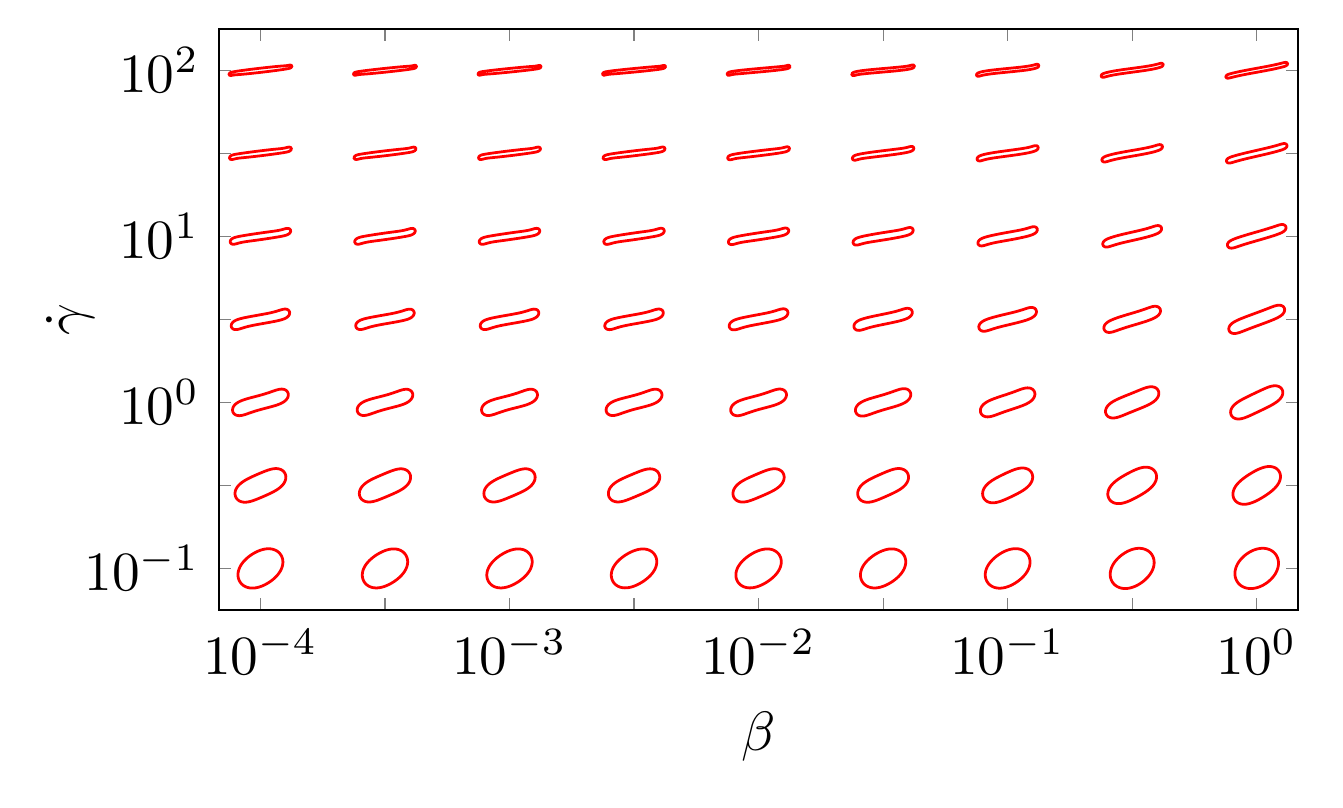
\begin{tikzpicture}[scale=2.0]

\pgfmathsetlengthmacro\MajorTickLength{
      \pgfkeysvalueof{/pgfplots/major tick length} * 0.5
    }

  \begin{axis}[
    major tick length=\MajorTickLength,
    compat=newest,
    axis equal image,
    xmin = 12,
    xmax = 64,
    ymin = 0,
    ymax = 28,
    xtick = {14,20,26,32,38,44,50,56,62},
    xticklabels = {$10^{-4}$,,$10^{-3}$,,$10^{-2}$,,
                    $10^{-1}$,,$10^{0}$},
    xlabel = {$\beta$},
    ytick = {2,6,10,14,18,22,26},
    yticklabels = {$10^{-1}$,,$10^{0}$,,$10^{1}$,,$10^2$},
    ylabel = {$\dot{\gamma}$},
    ylabel near ticks,
    ylabel shift = {-0.3cm},
  ]

%% beta = 1e-5,shear rate = 1e-1
%\addplot[red,line width=0.5pt] coordinates{
%(1.3082e+00,2.4832e+00)
%(1.2919e+00,2.4670e+00)
%(1.2754e+00,2.4502e+00)
%(1.2586e+00,2.4327e+00)
%(1.2413e+00,2.4139e+00)
%(1.2233e+00,2.3937e+00)
%(1.2044e+00,2.3719e+00)
%(1.1848e+00,2.3481e+00)
%(1.1643e+00,2.3223e+00)
%(1.1432e+00,2.2942e+00)
%(1.1215e+00,2.2638e+00)
%(1.0995e+00,2.2308e+00)
%(1.0773e+00,2.1952e+00)
%(1.0552e+00,2.1569e+00)
%(1.0337e+00,2.1158e+00)
%(1.0130e+00,2.0718e+00)
%(9.9361e-01,2.0249e+00)
%(9.7599e-01,1.9751e+00)
%(9.6068e-01,1.9226e+00)
%(9.4824e-01,1.8674e+00)
%(9.3928e-01,1.8097e+00)
%(9.3443e-01,1.7499e+00)
%(9.3429e-01,1.6884e+00)
%(9.3945e-01,1.6257e+00)
%(9.5045e-01,1.5624e+00)
%(9.6770e-01,1.4994e+00)
%(9.9148e-01,1.4374e+00)
%(1.0219e+00,1.3774e+00)
%(1.0589e+00,1.3204e+00)
%(1.1022e+00,1.2672e+00)
%(1.1513e+00,1.2186e+00)
%(1.2055e+00,1.1754e+00)
%(1.2640e+00,1.1380e+00)
%(1.3261e+00,1.1068e+00)
%(1.3908e+00,1.0818e+00)
%(1.4572e+00,1.0629e+00)
%(1.5246e+00,1.0500e+00)
%(1.5922e+00,1.0427e+00)
%(1.6594e+00,1.0405e+00)
%(1.7257e+00,1.0429e+00)
%(1.7908e+00,1.0495e+00)
%(1.8542e+00,1.0596e+00)
%(1.9158e+00,1.0729e+00)
%(1.9752e+00,1.0888e+00)
%(2.0324e+00,1.1068e+00)
%(2.0873e+00,1.1266e+00)
%(2.1398e+00,1.1478e+00)
%(2.1898e+00,1.1701e+00)
%(2.2373e+00,1.1931e+00)
%(2.2823e+00,1.2166e+00)
%(2.3248e+00,1.2402e+00)
%(2.3647e+00,1.2639e+00)
%(2.4022e+00,1.2873e+00)
%(2.4372e+00,1.3104e+00)
%(2.4699e+00,1.3329e+00)
%(2.5002e+00,1.3547e+00)
%(2.5283e+00,1.3758e+00)
%(2.5543e+00,1.3960e+00)
%(2.5783e+00,1.4154e+00)
%(2.6005e+00,1.4338e+00)
%(2.6210e+00,1.4515e+00)
%(2.6401e+00,1.4685e+00)
%(2.6581e+00,1.4848e+00)
%(2.6752e+00,1.5009e+00)
%(2.6918e+00,1.5168e+00)
%(2.7081e+00,1.5330e+00)
%(2.7246e+00,1.5498e+00)
%(2.7414e+00,1.5673e+00)
%(2.7587e+00,1.5861e+00)
%(2.7767e+00,1.6063e+00)
%(2.7956e+00,1.6281e+00)
%(2.8152e+00,1.6519e+00)
%(2.8357e+00,1.6777e+00)
%(2.8568e+00,1.7058e+00)
%(2.8785e+00,1.7362e+00)
%(2.9005e+00,1.7692e+00)
%(2.9227e+00,1.8048e+00)
%(2.9448e+00,1.8431e+00)
%(2.9663e+00,1.8842e+00)
%(2.9870e+00,1.9282e+00)
%(3.0064e+00,1.9751e+00)
%(3.0240e+00,2.0249e+00)
%(3.0393e+00,2.0774e+00)
%(3.0518e+00,2.1326e+00)
%(3.0607e+00,2.1903e+00)
%(3.0656e+00,2.2501e+00)
%(3.0657e+00,2.3116e+00)
%(3.0605e+00,2.3743e+00)
%(3.0496e+00,2.4376e+00)
%(3.0323e+00,2.5006e+00)
%(3.0085e+00,2.5626e+00)
%(2.9781e+00,2.6226e+00)
%(2.9411e+00,2.6796e+00)
%(2.8978e+00,2.7328e+00)
%(2.8487e+00,2.7814e+00)
%(2.7945e+00,2.8246e+00)
%(2.7360e+00,2.8620e+00)
%(2.6739e+00,2.8932e+00)
%(2.6092e+00,2.9182e+00)
%(2.5428e+00,2.9371e+00)
%(2.4754e+00,2.9500e+00)
%(2.4078e+00,2.9573e+00)
%(2.3406e+00,2.9595e+00)
%(2.2743e+00,2.9571e+00)
%(2.2092e+00,2.9505e+00)
%(2.1458e+00,2.9404e+00)
%(2.0842e+00,2.9271e+00)
%(2.0248e+00,2.9112e+00)
%(1.9676e+00,2.8932e+00)
%(1.9127e+00,2.8734e+00)
%(1.8602e+00,2.8522e+00)
%(1.8102e+00,2.8299e+00)
%(1.7627e+00,2.8069e+00)
%(1.7177e+00,2.7834e+00)
%(1.6752e+00,2.7598e+00)
%(1.6353e+00,2.7361e+00)
%(1.5978e+00,2.7127e+00)
%(1.5628e+00,2.6896e+00)
%(1.5301e+00,2.6671e+00)
%(1.4998e+00,2.6453e+00)
%(1.4717e+00,2.6242e+00)
%(1.4457e+00,2.6040e+00)
%(1.4217e+00,2.5846e+00)
%(1.3995e+00,2.5662e+00)
%(1.3790e+00,2.5485e+00)
%(1.3599e+00,2.5315e+00)
%(1.3419e+00,2.5152e+00)
%(1.3248e+00,2.4991e+00)
%(1.3082e+00,2.4832e+00)
%};
%
%% beta = 1e-5,shear rate = 1e-0.5
%\addplot[red,line width=0.5pt] coordinates{
%(2.5471e+00,6.8094e+00)
%(2.5246e+00,6.8052e+00)
%(2.5017e+00,6.8005e+00)
%(2.4780e+00,6.7951e+00)
%(2.4533e+00,6.7891e+00)
%(2.4272e+00,6.7823e+00)
%(2.3994e+00,6.7746e+00)
%(2.3700e+00,6.7658e+00)
%(2.3386e+00,6.7561e+00)
%(2.3054e+00,6.7451e+00)
%(2.2702e+00,6.7330e+00)
%(2.2329e+00,6.7196e+00)
%(2.1938e+00,6.7050e+00)
%(2.1526e+00,6.6891e+00)
%(2.1096e+00,6.6720e+00)
%(2.0647e+00,6.6537e+00)
%(2.0181e+00,6.6343e+00)
%(1.9697e+00,6.6136e+00)
%(1.9196e+00,6.5919e+00)
%(1.8680e+00,6.5690e+00)
%(1.8150e+00,6.5451e+00)
%(1.7606e+00,6.5202e+00)
%(1.7050e+00,6.4942e+00)
%(1.6484e+00,6.4671e+00)
%(1.5909e+00,6.4390e+00)
%(1.5327e+00,6.4096e+00)
%(1.4740e+00,6.3790e+00)
%(1.4150e+00,6.3470e+00)
%(1.3561e+00,6.3134e+00)
%(1.2974e+00,6.2782e+00)
%(1.2394e+00,6.2412e+00)
%(1.1824e+00,6.2020e+00)
%(1.1269e+00,6.1606e+00)
%(1.0733e+00,6.1166e+00)
%(1.0223e+00,6.0700e+00)
%(9.7444e-01,6.0205e+00)
%(9.3048e-01,5.9681e+00)
%(8.9122e-01,5.9129e+00)
%(8.5749e-01,5.8549e+00)
%(8.3016e-01,5.7946e+00)
%(8.1001e-01,5.7327e+00)
%(7.9770e-01,5.6699e+00)
%(7.9368e-01,5.6073e+00)
%(7.9806e-01,5.5462e+00)
%(8.1063e-01,5.4877e+00)
%(8.3076e-01,5.4332e+00)
%(8.5751e-01,5.3836e+00)
%(8.8969e-01,5.3395e+00)
%(9.2601e-01,5.3015e+00)
%(9.6514e-01,5.2695e+00)
%(1.0059e+00,5.2433e+00)
%(1.0472e+00,5.2224e+00)
%(1.0882e+00,5.2063e+00)
%(1.1282e+00,5.1943e+00)
%(1.1668e+00,5.1858e+00)
%(1.2037e+00,5.1801e+00)
%(1.2385e+00,5.1768e+00)
%(1.2713e+00,5.1753e+00)
%(1.3020e+00,5.1752e+00)
%(1.3308e+00,5.1762e+00)
%(1.3577e+00,5.1780e+00)
%(1.3831e+00,5.1805e+00)
%(1.4071e+00,5.1834e+00)
%(1.4303e+00,5.1868e+00)
%(1.4529e+00,5.1906e+00)
%(1.4754e+00,5.1948e+00)
%(1.4983e+00,5.1995e+00)
%(1.5220e+00,5.2049e+00)
%(1.5467e+00,5.2109e+00)
%(1.5728e+00,5.2177e+00)
%(1.6006e+00,5.2254e+00)
%(1.6300e+00,5.2342e+00)
%(1.6614e+00,5.2439e+00)
%(1.6946e+00,5.2549e+00)
%(1.7298e+00,5.2670e+00)
%(1.7671e+00,5.2804e+00)
%(1.8062e+00,5.2950e+00)
%(1.8474e+00,5.3109e+00)
%(1.8904e+00,5.3280e+00)
%(1.9353e+00,5.3463e+00)
%(1.9819e+00,5.3657e+00)
%(2.0303e+00,5.3864e+00)
%(2.0804e+00,5.4081e+00)
%(2.1320e+00,5.4310e+00)
%(2.1850e+00,5.4549e+00)
%(2.2394e+00,5.4798e+00)
%(2.2950e+00,5.5058e+00)
%(2.3516e+00,5.5329e+00)
%(2.4091e+00,5.5610e+00)
%(2.4673e+00,5.5904e+00)
%(2.5260e+00,5.6210e+00)
%(2.5850e+00,5.6530e+00)
%(2.6439e+00,5.6866e+00)
%(2.7026e+00,5.7218e+00)
%(2.7606e+00,5.7588e+00)
%(2.8176e+00,5.7980e+00)
%(2.8731e+00,5.8394e+00)
%(2.9267e+00,5.8834e+00)
%(2.9777e+00,5.9300e+00)
%(3.0256e+00,5.9795e+00)
%(3.0695e+00,6.0319e+00)
%(3.1088e+00,6.0871e+00)
%(3.1425e+00,6.1451e+00)
%(3.1698e+00,6.2054e+00)
%(3.1900e+00,6.2673e+00)
%(3.2023e+00,6.3301e+00)
%(3.2063e+00,6.3927e+00)
%(3.2019e+00,6.4538e+00)
%(3.1894e+00,6.5123e+00)
%(3.1692e+00,6.5668e+00)
%(3.1425e+00,6.6164e+00)
%(3.1103e+00,6.6605e+00)
%(3.0740e+00,6.6985e+00)
%(3.0349e+00,6.7305e+00)
%(2.9941e+00,6.7567e+00)
%(2.9528e+00,6.7776e+00)
%(2.9118e+00,6.7937e+00)
%(2.8718e+00,6.8057e+00)
%(2.8332e+00,6.8142e+00)
%(2.7963e+00,6.8199e+00)
%(2.7615e+00,6.8232e+00)
%(2.7287e+00,6.8247e+00)
%(2.6980e+00,6.8248e+00)
%(2.6692e+00,6.8238e+00)
%(2.6423e+00,6.8220e+00)
%(2.6169e+00,6.8195e+00)
%(2.5929e+00,6.8166e+00)
%(2.5697e+00,6.8132e+00)
%(2.5471e+00,6.8094e+00)
%};
%
%% beta = 1e-5,shear rate = 1e0
%\addplot[red,line width=0.5pt] coordinates{
%(7.4250e-01,9.8323e+00)
%(7.2969e-01,9.8134e+00)
%(7.1771e-01,9.7934e+00)
%(7.0652e-01,9.7720e+00)
%(6.9625e-01,9.7488e+00)
%(6.8719e-01,9.7235e+00)
%(6.7978e-01,9.6958e+00)
%(6.7465e-01,9.6656e+00)
%(6.7258e-01,9.6330e+00)
%(6.7446e-01,9.5982e+00)
%(6.8128e-01,9.5617e+00)
%(6.9398e-01,9.5245e+00)
%(7.1333e-01,9.4876e+00)
%(7.3977e-01,9.4527e+00)
%(7.7331e-01,9.4211e+00)
%(8.1347e-01,9.3944e+00)
%(8.5935e-01,9.3736e+00)
%(9.0980e-01,9.3596e+00)
%(9.6363e-01,9.3522e+00)
%(1.0198e+00,9.3513e+00)
%(1.0776e+00,9.3561e+00)
%(1.1364e+00,9.3658e+00)
%(1.1959e+00,9.3794e+00)
%(1.2562e+00,9.3960e+00)
%(1.3172e+00,9.4149e+00)
%(1.3788e+00,9.4352e+00)
%(1.4412e+00,9.4566e+00)
%(1.5044e+00,9.4784e+00)
%(1.5683e+00,9.5003e+00)
%(1.6329e+00,9.5222e+00)
%(1.6980e+00,9.5437e+00)
%(1.7636e+00,9.5648e+00)
%(1.8294e+00,9.5854e+00)
%(1.8955e+00,9.6055e+00)
%(1.9615e+00,9.6251e+00)
%(2.0274e+00,9.6442e+00)
%(2.0930e+00,9.6629e+00)
%(2.1580e+00,9.6812e+00)
%(2.2224e+00,9.6991e+00)
%(2.2859e+00,9.7167e+00)
%(2.3485e+00,9.7341e+00)
%(2.4099e+00,9.7513e+00)
%(2.4701e+00,9.7685e+00)
%(2.5288e+00,9.7855e+00)
%(2.5859e+00,9.8026e+00)
%(2.6412e+00,9.8197e+00)
%(2.6947e+00,9.8370e+00)
%(2.7462e+00,9.8545e+00)
%(2.7956e+00,9.8721e+00)
%(2.8427e+00,9.8901e+00)
%(2.8874e+00,9.9082e+00)
%(2.9297e+00,9.9267e+00)
%(2.9694e+00,9.9454e+00)
%(3.0066e+00,9.9642e+00)
%(3.0410e+00,9.9833e+00)
%(3.0729e+00,1.0002e+01)
%(3.1021e+00,1.0021e+01)
%(3.1288e+00,1.0040e+01)
%(3.1530e+00,1.0059e+01)
%(3.1749e+00,1.0077e+01)
%(3.1947e+00,1.0096e+01)
%(3.2126e+00,1.0114e+01)
%(3.2289e+00,1.0132e+01)
%(3.2438e+00,1.0149e+01)
%(3.2575e+00,1.0168e+01)
%(3.2703e+00,1.0187e+01)
%(3.2823e+00,1.0207e+01)
%(3.2935e+00,1.0228e+01)
%(3.3038e+00,1.0251e+01)
%(3.3128e+00,1.0277e+01)
%(3.3202e+00,1.0304e+01)
%(3.3253e+00,1.0334e+01)
%(3.3274e+00,1.0367e+01)
%(3.3255e+00,1.0402e+01)
%(3.3187e+00,1.0438e+01)
%(3.3060e+00,1.0476e+01)
%(3.2867e+00,1.0512e+01)
%(3.2602e+00,1.0547e+01)
%(3.2267e+00,1.0579e+01)
%(3.1865e+00,1.0606e+01)
%(3.1406e+00,1.0626e+01)
%(3.0902e+00,1.0640e+01)
%(3.0364e+00,1.0648e+01)
%(2.9802e+00,1.0649e+01)
%(2.9224e+00,1.0644e+01)
%(2.8636e+00,1.0634e+01)
%(2.8041e+00,1.0621e+01)
%(2.7438e+00,1.0604e+01)
%(2.6828e+00,1.0585e+01)
%(2.6212e+00,1.0565e+01)
%(2.5588e+00,1.0543e+01)
%(2.4956e+00,1.0522e+01)
%(2.4317e+00,1.0500e+01)
%(2.3671e+00,1.0478e+01)
%(2.3020e+00,1.0456e+01)
%(2.2364e+00,1.0435e+01)
%(2.1706e+00,1.0415e+01)
%(2.1045e+00,1.0394e+01)
%(2.0385e+00,1.0375e+01)
%(1.9726e+00,1.0356e+01)
%(1.9071e+00,1.0337e+01)
%(1.8420e+00,1.0319e+01)
%(1.7776e+00,1.0301e+01)
%(1.7141e+00,1.0283e+01)
%(1.6515e+00,1.0266e+01)
%(1.5901e+00,1.0249e+01)
%(1.5299e+00,1.0232e+01)
%(1.4712e+00,1.0214e+01)
%(1.4141e+00,1.0197e+01)
%(1.3588e+00,1.0180e+01)
%(1.3053e+00,1.0163e+01)
%(1.2538e+00,1.0146e+01)
%(1.2044e+00,1.0128e+01)
%(1.1573e+00,1.0110e+01)
%(1.1126e+00,1.0092e+01)
%(1.0703e+00,1.0073e+01)
%(1.0306e+00,1.0055e+01)
%(9.9345e-01,1.0036e+01)
%(9.5895e-01,1.0017e+01)
%(9.2710e-01,9.9977e+00)
%(8.9788e-01,9.9786e+00)
%(8.7120e-01,9.9597e+00)
%(8.4698e-01,9.9410e+00)
%(8.2507e-01,9.9225e+00)
%(8.0527e-01,9.9043e+00)
%(7.8737e-01,9.8863e+00)
%(7.7111e-01,9.8685e+00)
%(7.5623e-01,9.8505e+00)
%(7.4250e-01,9.8323e+00)
%};
%
%% beta = 1e-5,shear rate = 1e0.5
%\addplot[red,line width=0.5pt] coordinates{
%(1.3090e+00,1.3613e+01)
%(1.3310e+00,1.3619e+01)
%(1.3535e+00,1.3625e+01)
%(1.3769e+00,1.3631e+01)
%(1.4014e+00,1.3637e+01)
%(1.4275e+00,1.3644e+01)
%(1.4553e+00,1.3651e+01)
%(1.4851e+00,1.3658e+01)
%(1.5169e+00,1.3665e+01)
%(1.5509e+00,1.3673e+01)
%(1.5871e+00,1.3681e+01)
%(1.6256e+00,1.3689e+01)
%(1.6663e+00,1.3697e+01)
%(1.7092e+00,1.3706e+01)
%(1.7544e+00,1.3715e+01)
%(1.8017e+00,1.3724e+01)
%(1.8511e+00,1.3734e+01)
%(1.9025e+00,1.3744e+01)
%(1.9558e+00,1.3754e+01)
%(2.0109e+00,1.3765e+01)
%(2.0678e+00,1.3776e+01)
%(2.1262e+00,1.3787e+01)
%(2.1862e+00,1.3798e+01)
%(2.2475e+00,1.3810e+01)
%(2.3100e+00,1.3823e+01)
%(2.3736e+00,1.3835e+01)
%(2.4382e+00,1.3848e+01)
%(2.5036e+00,1.3861e+01)
%(2.5696e+00,1.3875e+01)
%(2.6362e+00,1.3889e+01)
%(2.7031e+00,1.3904e+01)
%(2.7702e+00,1.3919e+01)
%(2.8373e+00,1.3935e+01)
%(2.9041e+00,1.3952e+01)
%(2.9703e+00,1.3970e+01)
%(3.0357e+00,1.3991e+01)
%(3.0998e+00,1.4014e+01)
%(3.1620e+00,1.4040e+01)
%(3.2213e+00,1.4070e+01)
%(3.2763e+00,1.4106e+01)
%(3.3251e+00,1.4149e+01)
%(3.3648e+00,1.4199e+01)
%(3.3917e+00,1.4255e+01)
%(3.4021e+00,1.4315e+01)
%(3.3939e+00,1.4374e+01)
%(3.3679e+00,1.4425e+01)
%(3.3282e+00,1.4464e+01)
%(3.2806e+00,1.4490e+01)
%(3.2301e+00,1.4504e+01)
%(3.1800e+00,1.4508e+01)
%(3.1319e+00,1.4505e+01)
%(3.0863e+00,1.4498e+01)
%(3.0435e+00,1.4489e+01)
%(3.0032e+00,1.4479e+01)
%(2.9653e+00,1.4468e+01)
%(2.9298e+00,1.4458e+01)
%(2.8965e+00,1.4447e+01)
%(2.8652e+00,1.4438e+01)
%(2.8360e+00,1.4429e+01)
%(2.8086e+00,1.4421e+01)
%(2.7829e+00,1.4413e+01)
%(2.7585e+00,1.4406e+01)
%(2.7354e+00,1.4399e+01)
%(2.7130e+00,1.4393e+01)
%(2.6910e+00,1.4387e+01)
%(2.6690e+00,1.4381e+01)
%(2.6465e+00,1.4375e+01)
%(2.6231e+00,1.4369e+01)
%(2.5986e+00,1.4363e+01)
%(2.5725e+00,1.4356e+01)
%(2.5447e+00,1.4349e+01)
%(2.5149e+00,1.4342e+01)
%(2.4831e+00,1.4335e+01)
%(2.4491e+00,1.4327e+01)
%(2.4129e+00,1.4319e+01)
%(2.3744e+00,1.4311e+01)
%(2.3337e+00,1.4303e+01)
%(2.2908e+00,1.4294e+01)
%(2.2456e+00,1.4285e+01)
%(2.1983e+00,1.4276e+01)
%(2.1489e+00,1.4266e+01)
%(2.0975e+00,1.4256e+01)
%(2.0442e+00,1.4246e+01)
%(1.9891e+00,1.4235e+01)
%(1.9322e+00,1.4224e+01)
%(1.8738e+00,1.4213e+01)
%(1.8138e+00,1.4202e+01)
%(1.7525e+00,1.4190e+01)
%(1.6900e+00,1.4177e+01)
%(1.6264e+00,1.4165e+01)
%(1.5618e+00,1.4152e+01)
%(1.4964e+00,1.4139e+01)
%(1.4304e+00,1.4125e+01)
%(1.3638e+00,1.4111e+01)
%(1.2969e+00,1.4096e+01)
%(1.2298e+00,1.4081e+01)
%(1.1627e+00,1.4065e+01)
%(1.0959e+00,1.4048e+01)
%(1.0297e+00,1.4030e+01)
%(9.6426e-01,1.4009e+01)
%(9.0016e-01,1.3986e+01)
%(8.3801e-01,1.3960e+01)
%(7.7872e-01,1.3930e+01)
%(7.2367e-01,1.3894e+01)
%(6.7488e-01,1.3851e+01)
%(6.3523e-01,1.3801e+01)
%(6.0833e-01,1.3745e+01)
%(5.9787e-01,1.3685e+01)
%(6.0610e-01,1.3626e+01)
%(6.3214e-01,1.3575e+01)
%(6.7181e-01,1.3536e+01)
%(7.1940e-01,1.3510e+01)
%(7.6988e-01,1.3496e+01)
%(8.1999e-01,1.3492e+01)
%(8.6812e-01,1.3495e+01)
%(9.1367e-01,1.3502e+01)
%(9.5655e-01,1.3511e+01)
%(9.9684e-01,1.3521e+01)
%(1.0347e+00,1.3532e+01)
%(1.0702e+00,1.3542e+01)
%(1.1035e+00,1.3553e+01)
%(1.1348e+00,1.3562e+01)
%(1.1640e+00,1.3571e+01)
%(1.1914e+00,1.3579e+01)
%(1.2171e+00,1.3587e+01)
%(1.2415e+00,1.3594e+01)
%(1.2646e+00,1.3601e+01)
%(1.2870e+00,1.3607e+01)
%(1.3090e+00,1.3613e+01)
%};
%
%% beta = 1e-5,shear rate = 1e1
%\addplot[red,line width=0.5pt] coordinates{
%(2.3881e+00,1.7877e+01)
%(2.4105e+00,1.7881e+01)
%(2.4333e+00,1.7885e+01)
%(2.4570e+00,1.7890e+01)
%(2.4818e+00,1.7895e+01)
%(2.5082e+00,1.7900e+01)
%(2.5362e+00,1.7905e+01)
%(2.5662e+00,1.7911e+01)
%(2.5982e+00,1.7918e+01)
%(2.6323e+00,1.7925e+01)
%(2.6686e+00,1.7932e+01)
%(2.7071e+00,1.7940e+01)
%(2.7478e+00,1.7949e+01)
%(2.7906e+00,1.7958e+01)
%(2.8356e+00,1.7968e+01)
%(2.8827e+00,1.7978e+01)
%(2.9317e+00,1.7989e+01)
%(2.9826e+00,1.8001e+01)
%(3.0353e+00,1.8014e+01)
%(3.0896e+00,1.8028e+01)
%(3.1452e+00,1.8044e+01)
%(3.2018e+00,1.8063e+01)
%(3.2587e+00,1.8085e+01)
%(3.3147e+00,1.8112e+01)
%(3.3675e+00,1.8147e+01)
%(3.4125e+00,1.8194e+01)
%(3.4411e+00,1.8253e+01)
%(3.4419e+00,1.8319e+01)
%(3.4090e+00,1.8376e+01)
%(3.3511e+00,1.8411e+01)
%(3.2836e+00,1.8421e+01)
%(3.2152e+00,1.8415e+01)
%(3.1477e+00,1.8401e+01)
%(3.0808e+00,1.8384e+01)
%(3.0140e+00,1.8368e+01)
%(2.9472e+00,1.8353e+01)
%(2.8805e+00,1.8340e+01)
%(2.8142e+00,1.8328e+01)
%(2.7485e+00,1.8316e+01)
%(2.6835e+00,1.8306e+01)
%(2.6195e+00,1.8295e+01)
%(2.5566e+00,1.8285e+01)
%(2.4950e+00,1.8276e+01)
%(2.4347e+00,1.8266e+01)
%(2.3760e+00,1.8257e+01)
%(2.3189e+00,1.8248e+01)
%(2.2635e+00,1.8239e+01)
%(2.2099e+00,1.8230e+01)
%(2.1583e+00,1.8222e+01)
%(2.1088e+00,1.8213e+01)
%(2.0613e+00,1.8205e+01)
%(2.0159e+00,1.8197e+01)
%(1.9727e+00,1.8190e+01)
%(1.9318e+00,1.8182e+01)
%(1.8931e+00,1.8176e+01)
%(1.8566e+00,1.8169e+01)
%(1.8224e+00,1.8163e+01)
%(1.7903e+00,1.8157e+01)
%(1.7602e+00,1.8151e+01)
%(1.7321e+00,1.8146e+01)
%(1.7057e+00,1.8141e+01)
%(1.6808e+00,1.8137e+01)
%(1.6571e+00,1.8132e+01)
%(1.6343e+00,1.8128e+01)
%(1.6119e+00,1.8123e+01)
%(1.5895e+00,1.8119e+01)
%(1.5667e+00,1.8115e+01)
%(1.5430e+00,1.8110e+01)
%(1.5182e+00,1.8105e+01)
%(1.4918e+00,1.8100e+01)
%(1.4638e+00,1.8095e+01)
%(1.4338e+00,1.8089e+01)
%(1.4018e+00,1.8082e+01)
%(1.3677e+00,1.8075e+01)
%(1.3314e+00,1.8068e+01)
%(1.2929e+00,1.8060e+01)
%(1.2522e+00,1.8051e+01)
%(1.2094e+00,1.8042e+01)
%(1.1644e+00,1.8032e+01)
%(1.1173e+00,1.8022e+01)
%(1.0683e+00,1.8011e+01)
%(1.0174e+00,1.7999e+01)
%(9.6467e-01,1.7986e+01)
%(9.1039e-01,1.7972e+01)
%(8.5478e-01,1.7956e+01)
%(7.9822e-01,1.7937e+01)
%(7.4133e-01,1.7915e+01)
%(6.8532e-01,1.7888e+01)
%(6.3251e-01,1.7853e+01)
%(5.8755e-01,1.7806e+01)
%(5.5890e-01,1.7747e+01)
%(5.5806e-01,1.7681e+01)
%(5.9103e-01,1.7624e+01)
%(6.4895e-01,1.7589e+01)
%(7.1640e-01,1.7579e+01)
%(7.8479e-01,1.7585e+01)
%(8.5226e-01,1.7599e+01)
%(9.1921e-01,1.7616e+01)
%(9.8604e-01,1.7632e+01)
%(1.0528e+00,1.7647e+01)
%(1.1195e+00,1.7660e+01)
%(1.1858e+00,1.7672e+01)
%(1.2515e+00,1.7684e+01)
%(1.3165e+00,1.7694e+01)
%(1.3805e+00,1.7705e+01)
%(1.4434e+00,1.7715e+01)
%(1.5050e+00,1.7724e+01)
%(1.5653e+00,1.7734e+01)
%(1.6240e+00,1.7743e+01)
%(1.6811e+00,1.7752e+01)
%(1.7365e+00,1.7761e+01)
%(1.7901e+00,1.7770e+01)
%(1.8417e+00,1.7778e+01)
%(1.8912e+00,1.7787e+01)
%(1.9387e+00,1.7795e+01)
%(1.9841e+00,1.7803e+01)
%(2.0273e+00,1.7810e+01)
%(2.0682e+00,1.7818e+01)
%(2.1069e+00,1.7824e+01)
%(2.1434e+00,1.7831e+01)
%(2.1776e+00,1.7837e+01)
%(2.2097e+00,1.7843e+01)
%(2.2398e+00,1.7849e+01)
%(2.2679e+00,1.7854e+01)
%(2.2943e+00,1.7859e+01)
%(2.3192e+00,1.7863e+01)
%(2.3429e+00,1.7868e+01)
%(2.3657e+00,1.7872e+01)
%(2.3881e+00,1.7877e+01)
%};
%
%% beta = 1e-5,shear rate = 1e1.5
%\addplot[red,line width=0.5pt] coordinates{
%(3.3517e+00,2.2105e+01)
%(3.3727e+00,2.2114e+01)
%(3.3936e+00,2.2124e+01)
%(3.4143e+00,2.2136e+01)
%(3.4347e+00,2.2151e+01)
%(3.4539e+00,2.2170e+01)
%(3.4703e+00,2.2193e+01)
%(3.4812e+00,2.2222e+01)
%(3.4825e+00,2.2254e+01)
%(3.4705e+00,2.2287e+01)
%(3.4445e+00,2.2313e+01)
%(3.4084e+00,2.2328e+01)
%(3.3671e+00,2.2332e+01)
%(3.3235e+00,2.2328e+01)
%(3.2783e+00,2.2319e+01)
%(3.2311e+00,2.2309e+01)
%(3.1818e+00,2.2299e+01)
%(3.1303e+00,2.2290e+01)
%(3.0766e+00,2.2282e+01)
%(3.0210e+00,2.2275e+01)
%(2.9636e+00,2.2268e+01)
%(2.9044e+00,2.2261e+01)
%(2.8438e+00,2.2254e+01)
%(2.7818e+00,2.2247e+01)
%(2.7185e+00,2.2240e+01)
%(2.6541e+00,2.2232e+01)
%(2.5887e+00,2.2224e+01)
%(2.5226e+00,2.2216e+01)
%(2.4557e+00,2.2208e+01)
%(2.3882e+00,2.2199e+01)
%(2.3203e+00,2.2190e+01)
%(2.2522e+00,2.2180e+01)
%(2.1839e+00,2.2171e+01)
%(2.1157e+00,2.2161e+01)
%(2.0476e+00,2.2152e+01)
%(1.9799e+00,2.2142e+01)
%(1.9126e+00,2.2132e+01)
%(1.8459e+00,2.2122e+01)
%(1.7799e+00,2.2112e+01)
%(1.7149e+00,2.2102e+01)
%(1.6508e+00,2.2092e+01)
%(1.5879e+00,2.2082e+01)
%(1.5263e+00,2.2072e+01)
%(1.4661e+00,2.2062e+01)
%(1.4074e+00,2.2052e+01)
%(1.3503e+00,2.2042e+01)
%(1.2950e+00,2.2033e+01)
%(1.2415e+00,2.2024e+01)
%(1.1900e+00,2.2015e+01)
%(1.1405e+00,2.2006e+01)
%(1.0931e+00,2.1997e+01)
%(1.0478e+00,2.1989e+01)
%(1.0047e+00,2.1981e+01)
%(9.6388e-01,2.1973e+01)
%(9.2529e-01,2.1965e+01)
%(8.8896e-01,2.1958e+01)
%(8.5487e-01,2.1951e+01)
%(8.2295e-01,2.1944e+01)
%(7.9313e-01,2.1937e+01)
%(7.6529e-01,2.1931e+01)
%(7.3927e-01,2.1924e+01)
%(7.1484e-01,2.1917e+01)
%(6.9174e-01,2.1910e+01)
%(6.6967e-01,2.1903e+01)
%(6.4828e-01,2.1895e+01)
%(6.2728e-01,2.1886e+01)
%(6.0643e-01,2.1876e+01)
%(5.8570e-01,2.1864e+01)
%(5.6534e-01,2.1849e+01)
%(5.4613e-01,2.1830e+01)
%(5.2968e-01,2.1807e+01)
%(5.1882e-01,2.1778e+01)
%(5.1752e-01,2.1746e+01)
%(5.2953e-01,2.1713e+01)
%(5.5546e-01,2.1687e+01)
%(5.9156e-01,2.1672e+01)
%(6.3286e-01,2.1668e+01)
%(6.7647e-01,2.1672e+01)
%(7.2172e-01,2.1681e+01)
%(7.6887e-01,2.1691e+01)
%(8.1818e-01,2.1701e+01)
%(8.6971e-01,2.1710e+01)
%(9.2336e-01,2.1718e+01)
%(9.7900e-01,2.1725e+01)
%(1.0365e+00,2.1732e+01)
%(1.0956e+00,2.1739e+01)
%(1.1562e+00,2.1746e+01)
%(1.2182e+00,2.1753e+01)
%(1.2815e+00,2.1760e+01)
%(1.3459e+00,2.1768e+01)
%(1.4113e+00,2.1776e+01)
%(1.4775e+00,2.1784e+01)
%(1.5443e+00,2.1792e+01)
%(1.6118e+00,2.1801e+01)
%(1.6797e+00,2.1810e+01)
%(1.7478e+00,2.1820e+01)
%(1.8161e+00,2.1829e+01)
%(1.8843e+00,2.1839e+01)
%(1.9524e+00,2.1848e+01)
%(2.0201e+00,2.1858e+01)
%(2.0874e+00,2.1868e+01)
%(2.1541e+00,2.1878e+01)
%(2.2201e+00,2.1888e+01)
%(2.2851e+00,2.1898e+01)
%(2.3492e+00,2.1908e+01)
%(2.4121e+00,2.1918e+01)
%(2.4737e+00,2.1928e+01)
%(2.5339e+00,2.1938e+01)
%(2.5926e+00,2.1948e+01)
%(2.6497e+00,2.1958e+01)
%(2.7050e+00,2.1967e+01)
%(2.7585e+00,2.1976e+01)
%(2.8100e+00,2.1985e+01)
%(2.8595e+00,2.1994e+01)
%(2.9069e+00,2.2003e+01)
%(2.9522e+00,2.2011e+01)
%(2.9953e+00,2.2019e+01)
%(3.0361e+00,2.2027e+01)
%(3.0747e+00,2.2035e+01)
%(3.1110e+00,2.2042e+01)
%(3.1451e+00,2.2049e+01)
%(3.1771e+00,2.2056e+01)
%(3.2069e+00,2.2063e+01)
%(3.2347e+00,2.2069e+01)
%(3.2607e+00,2.2076e+01)
%(3.2852e+00,2.2083e+01)
%(3.3083e+00,2.2090e+01)
%(3.3303e+00,2.2097e+01)
%(3.3517e+00,2.2105e+01)
%};
%
%% beta = 1e-5,shear rate = 1e2
%\addplot[red,line width=0.5pt] coordinates{
%(1.1063e+00,2.5989e+01)
%(1.0841e+00,2.5984e+01)
%(1.0614e+00,2.5979e+01)
%(1.0381e+00,2.5974e+01)
%(1.0134e+00,2.5969e+01)
%(9.8737e-01,2.5963e+01)
%(9.5954e-01,2.5956e+01)
%(9.2996e-01,2.5950e+01)
%(8.9827e-01,2.5942e+01)
%(8.6465e-01,2.5934e+01)
%(8.2879e-01,2.5925e+01)
%(7.9097e-01,2.5915e+01)
%(7.5094e-01,2.5904e+01)
%(7.0915e-01,2.5892e+01)
%(6.6544e-01,2.5877e+01)
%(6.2084e-01,2.5860e+01)
%(5.7627e-01,2.5837e+01)
%(5.3697e-01,2.5803e+01)
%(5.1549e-01,2.5754e+01)
%(5.3367e-01,2.5704e+01)
%(5.8473e-01,2.5678e+01)
%(6.4358e-01,2.5675e+01)
%(7.0440e-01,2.5679e+01)
%(7.6628e-01,2.5683e+01)
%(8.2968e-01,2.5686e+01)
%(8.9395e-01,2.5691e+01)
%(9.5934e-01,2.5696e+01)
%(1.0253e+00,2.5703e+01)
%(1.0922e+00,2.5710e+01)
%(1.1593e+00,2.5717e+01)
%(1.2270e+00,2.5725e+01)
%(1.2948e+00,2.5734e+01)
%(1.3628e+00,2.5743e+01)
%(1.4307e+00,2.5752e+01)
%(1.4985e+00,2.5762e+01)
%(1.5658e+00,2.5772e+01)
%(1.6328e+00,2.5782e+01)
%(1.6990e+00,2.5792e+01)
%(1.7647e+00,2.5802e+01)
%(1.8293e+00,2.5813e+01)
%(1.8930e+00,2.5823e+01)
%(1.9555e+00,2.5833e+01)
%(2.0168e+00,2.5844e+01)
%(2.0767e+00,2.5854e+01)
%(2.1351e+00,2.5864e+01)
%(2.1918e+00,2.5874e+01)
%(2.2468e+00,2.5884e+01)
%(2.2999e+00,2.5894e+01)
%(2.3512e+00,2.5903e+01)
%(2.4005e+00,2.5912e+01)
%(2.4477e+00,2.5921e+01)
%(2.4927e+00,2.5930e+01)
%(2.5356e+00,2.5938e+01)
%(2.5762e+00,2.5946e+01)
%(2.6147e+00,2.5953e+01)
%(2.6509e+00,2.5960e+01)
%(2.6849e+00,2.5967e+01)
%(2.7167e+00,2.5974e+01)
%(2.7466e+00,2.5980e+01)
%(2.7745e+00,2.5985e+01)
%(2.8007e+00,2.5991e+01)
%(2.8253e+00,2.5996e+01)
%(2.8489e+00,2.6001e+01)
%(2.8715e+00,2.6006e+01)
%(2.8937e+00,2.6011e+01)
%(2.9159e+00,2.6016e+01)
%(2.9385e+00,2.6021e+01)
%(2.9619e+00,2.6026e+01)
%(2.9866e+00,2.6031e+01)
%(3.0126e+00,2.6037e+01)
%(3.0405e+00,2.6044e+01)
%(3.0700e+00,2.6050e+01)
%(3.1017e+00,2.6058e+01)
%(3.1353e+00,2.6066e+01)
%(3.1712e+00,2.6075e+01)
%(3.2090e+00,2.6085e+01)
%(3.2491e+00,2.6096e+01)
%(3.2908e+00,2.6108e+01)
%(3.3346e+00,2.6123e+01)
%(3.3792e+00,2.6140e+01)
%(3.4237e+00,2.6163e+01)
%(3.4630e+00,2.6197e+01)
%(3.4845e+00,2.6246e+01)
%(3.4663e+00,2.6296e+01)
%(3.4153e+00,2.6322e+01)
%(3.3564e+00,2.6325e+01)
%(3.2956e+00,2.6321e+01)
%(3.2337e+00,2.6317e+01)
%(3.1703e+00,2.6314e+01)
%(3.1061e+00,2.6309e+01)
%(3.0407e+00,2.6304e+01)
%(2.9747e+00,2.6297e+01)
%(2.9078e+00,2.6290e+01)
%(2.8407e+00,2.6283e+01)
%(2.7730e+00,2.6275e+01)
%(2.7052e+00,2.6266e+01)
%(2.6372e+00,2.6257e+01)
%(2.5693e+00,2.6248e+01)
%(2.5015e+00,2.6238e+01)
%(2.4342e+00,2.6228e+01)
%(2.3672e+00,2.6218e+01)
%(2.3010e+00,2.6208e+01)
%(2.2353e+00,2.6198e+01)
%(2.1707e+00,2.6187e+01)
%(2.1070e+00,2.6177e+01)
%(2.0445e+00,2.6167e+01)
%(1.9832e+00,2.6156e+01)
%(1.9233e+00,2.6146e+01)
%(1.8649e+00,2.6136e+01)
%(1.8082e+00,2.6126e+01)
%(1.7532e+00,2.6116e+01)
%(1.7001e+00,2.6106e+01)
%(1.6488e+00,2.6097e+01)
%(1.5995e+00,2.6088e+01)
%(1.5523e+00,2.6079e+01)
%(1.5073e+00,2.6070e+01)
%(1.4644e+00,2.6062e+01)
%(1.4238e+00,2.6054e+01)
%(1.3853e+00,2.6047e+01)
%(1.3491e+00,2.6040e+01)
%(1.3151e+00,2.6033e+01)
%(1.2833e+00,2.6026e+01)
%(1.2534e+00,2.6020e+01)
%(1.2255e+00,2.6015e+01)
%(1.1993e+00,2.6009e+01)
%(1.1747e+00,2.6004e+01)
%(1.1511e+00,2.5999e+01)
%(1.1285e+00,2.5994e+01)
%(1.1063e+00,2.5989e+01)
%};
%
%% beta = 1e-4.5,shear rate = 1e-1
%\addplot[red,line width=0.5pt] coordinates{
%(7.8403e+00,2.8763e+00)
%(7.8191e+00,2.8675e+00)
%(7.7976e+00,2.8581e+00)
%(7.7755e+00,2.8480e+00)
%(7.7524e+00,2.8370e+00)
%(7.7282e+00,2.8249e+00)
%(7.7026e+00,2.8116e+00)
%(7.6755e+00,2.7968e+00)
%(7.6469e+00,2.7805e+00)
%(7.6168e+00,2.7624e+00)
%(7.5852e+00,2.7425e+00)
%(7.5521e+00,2.7206e+00)
%(7.5177e+00,2.6966e+00)
%(7.4821e+00,2.6704e+00)
%(7.4455e+00,2.6418e+00)
%(7.4081e+00,2.6108e+00)
%(7.3700e+00,2.5772e+00)
%(7.3315e+00,2.5411e+00)
%(7.2929e+00,2.5023e+00)
%(7.2545e+00,2.4608e+00)
%(7.2165e+00,2.4165e+00)
%(7.1794e+00,2.3693e+00)
%(7.1434e+00,2.3194e+00)
%(7.1091e+00,2.2666e+00)
%(7.0768e+00,2.2111e+00)
%(7.0471e+00,2.1529e+00)
%(7.0203e+00,2.0921e+00)
%(6.9971e+00,2.0290e+00)
%(6.9780e+00,1.9637e+00)
%(6.9635e+00,1.8966e+00)
%(6.9541e+00,1.8282e+00)
%(6.9503e+00,1.7590e+00)
%(6.9524e+00,1.6895e+00)
%(6.9607e+00,1.6206e+00)
%(6.9754e+00,1.5528e+00)
%(6.9964e+00,1.4870e+00)
%(7.0236e+00,1.4241e+00)
%(7.0566e+00,1.3646e+00)
%(7.0949e+00,1.3094e+00)
%(7.1380e+00,1.2588e+00)
%(7.1850e+00,1.2134e+00)
%(7.2352e+00,1.1734e+00)
%(7.2877e+00,1.1387e+00)
%(7.3418e+00,1.1095e+00)
%(7.3968e+00,1.0854e+00)
%(7.4519e+00,1.0661e+00)
%(7.5065e+00,1.0514e+00)
%(7.5602e+00,1.0408e+00)
%(7.6125e+00,1.0338e+00)
%(7.6631e+00,1.0300e+00)
%(7.7117e+00,1.0289e+00)
%(7.7581e+00,1.0301e+00)
%(7.8022e+00,1.0332e+00)
%(7.8439e+00,1.0378e+00)
%(7.8831e+00,1.0437e+00)
%(7.9199e+00,1.0504e+00)
%(7.9542e+00,1.0578e+00)
%(7.9862e+00,1.0656e+00)
%(8.0159e+00,1.0737e+00)
%(8.0436e+00,1.0820e+00)
%(8.0694e+00,1.0902e+00)
%(8.0935e+00,1.0985e+00)
%(8.1164e+00,1.1067e+00)
%(8.1383e+00,1.1151e+00)
%(8.1597e+00,1.1237e+00)
%(8.1809e+00,1.1325e+00)
%(8.2024e+00,1.1419e+00)
%(8.2245e+00,1.1520e+00)
%(8.2476e+00,1.1630e+00)
%(8.2718e+00,1.1751e+00)
%(8.2974e+00,1.1884e+00)
%(8.3245e+00,1.2032e+00)
%(8.3531e+00,1.2195e+00)
%(8.3832e+00,1.2376e+00)
%(8.4148e+00,1.2575e+00)
%(8.4479e+00,1.2794e+00)
%(8.4823e+00,1.3034e+00)
%(8.5179e+00,1.3296e+00)
%(8.5545e+00,1.3582e+00)
%(8.5919e+00,1.3892e+00)
%(8.6300e+00,1.4228e+00)
%(8.6685e+00,1.4589e+00)
%(8.7071e+00,1.4977e+00)
%(8.7455e+00,1.5392e+00)
%(8.7835e+00,1.5835e+00)
%(8.8206e+00,1.6307e+00)
%(8.8566e+00,1.6806e+00)
%(8.8909e+00,1.7334e+00)
%(8.9232e+00,1.7889e+00)
%(8.9529e+00,1.8471e+00)
%(8.9797e+00,1.9079e+00)
%(9.0029e+00,1.9710e+00)
%(9.0220e+00,2.0363e+00)
%(9.0365e+00,2.1034e+00)
%(9.0459e+00,2.1718e+00)
%(9.0497e+00,2.2410e+00)
%(9.0476e+00,2.3105e+00)
%(9.0393e+00,2.3794e+00)
%(9.0246e+00,2.4472e+00)
%(9.0036e+00,2.5130e+00)
%(8.9764e+00,2.5759e+00)
%(8.9434e+00,2.6354e+00)
%(8.9051e+00,2.6906e+00)
%(8.8620e+00,2.7412e+00)
%(8.8150e+00,2.7866e+00)
%(8.7648e+00,2.8266e+00)
%(8.7123e+00,2.8613e+00)
%(8.6582e+00,2.8905e+00)
%(8.6032e+00,2.9146e+00)
%(8.5481e+00,2.9339e+00)
%(8.4935e+00,2.9486e+00)
%(8.4398e+00,2.9592e+00)
%(8.3875e+00,2.9662e+00)
%(8.3369e+00,2.9700e+00)
%(8.2883e+00,2.9711e+00)
%(8.2419e+00,2.9699e+00)
%(8.1978e+00,2.9668e+00)
%(8.1561e+00,2.9622e+00)
%(8.1169e+00,2.9563e+00)
%(8.0801e+00,2.9496e+00)
%(8.0458e+00,2.9422e+00)
%(8.0138e+00,2.9344e+00)
%(7.9841e+00,2.9263e+00)
%(7.9564e+00,2.9180e+00)
%(7.9306e+00,2.9098e+00)
%(7.9065e+00,2.9015e+00)
%(7.8836e+00,2.8933e+00)
%(7.8617e+00,2.8849e+00)
%(7.8403e+00,2.8763e+00)
%};
%
%% beta = 1e-4.5,shear rate = 1e-0.5
%\addplot[red,line width=0.5pt] coordinates{
%(6.8580e+00,5.8393e+00)
%(6.8488e+00,5.8182e+00)
%(6.8402e+00,5.7963e+00)
%(6.8322e+00,5.7734e+00)
%(6.8248e+00,5.7490e+00)
%(6.8181e+00,5.7227e+00)
%(6.8124e+00,5.6944e+00)
%(6.8081e+00,5.6639e+00)
%(6.8055e+00,5.6311e+00)
%(6.8052e+00,5.5960e+00)
%(6.8077e+00,5.5587e+00)
%(6.8136e+00,5.5195e+00)
%(6.8237e+00,5.4788e+00)
%(6.8386e+00,5.4372e+00)
%(6.8587e+00,5.3954e+00)
%(6.8846e+00,5.3542e+00)
%(6.9165e+00,5.3148e+00)
%(6.9543e+00,5.2780e+00)
%(6.9979e+00,5.2450e+00)
%(7.0468e+00,5.2165e+00)
%(7.1002e+00,5.1932e+00)
%(7.1576e+00,5.1756e+00)
%(7.2179e+00,5.1638e+00)
%(7.2806e+00,5.1576e+00)
%(7.3448e+00,5.1569e+00)
%(7.4100e+00,5.1612e+00)
%(7.4758e+00,5.1700e+00)
%(7.5419e+00,5.1826e+00)
%(7.6080e+00,5.1986e+00)
%(7.6740e+00,5.2174e+00)
%(7.7398e+00,5.2385e+00)
%(7.8052e+00,5.2615e+00)
%(7.8703e+00,5.2860e+00)
%(7.9348e+00,5.3117e+00)
%(7.9988e+00,5.3384e+00)
%(8.0622e+00,5.3658e+00)
%(8.1248e+00,5.3939e+00)
%(8.1866e+00,5.4224e+00)
%(8.2474e+00,5.4512e+00)
%(8.3071e+00,5.4804e+00)
%(8.3655e+00,5.5098e+00)
%(8.4225e+00,5.5394e+00)
%(8.4779e+00,5.5692e+00)
%(8.5317e+00,5.5991e+00)
%(8.5836e+00,5.6292e+00)
%(8.6336e+00,5.6593e+00)
%(8.6815e+00,5.6895e+00)
%(8.7271e+00,5.7198e+00)
%(8.7703e+00,5.7500e+00)
%(8.8112e+00,5.7801e+00)
%(8.8495e+00,5.8100e+00)
%(8.8853e+00,5.8397e+00)
%(8.9184e+00,5.8689e+00)
%(8.9490e+00,5.8977e+00)
%(8.9769e+00,5.9258e+00)
%(9.0024e+00,5.9531e+00)
%(9.0254e+00,5.9797e+00)
%(9.0461e+00,6.0052e+00)
%(9.0647e+00,6.0298e+00)
%(9.0813e+00,6.0535e+00)
%(9.0961e+00,6.0761e+00)
%(9.1094e+00,6.0980e+00)
%(9.1213e+00,6.1192e+00)
%(9.1321e+00,6.1400e+00)
%(9.1420e+00,6.1607e+00)
%(9.1512e+00,6.1818e+00)
%(9.1598e+00,6.2037e+00)
%(9.1678e+00,6.2266e+00)
%(9.1752e+00,6.2510e+00)
%(9.1819e+00,6.2773e+00)
%(9.1876e+00,6.3056e+00)
%(9.1919e+00,6.3361e+00)
%(9.1945e+00,6.3689e+00)
%(9.1948e+00,6.4040e+00)
%(9.1923e+00,6.4413e+00)
%(9.1864e+00,6.4805e+00)
%(9.1763e+00,6.5212e+00)
%(9.1614e+00,6.5628e+00)
%(9.1413e+00,6.6046e+00)
%(9.1154e+00,6.6458e+00)
%(9.0835e+00,6.6852e+00)
%(9.0457e+00,6.7220e+00)
%(9.0021e+00,6.7550e+00)
%(8.9532e+00,6.7835e+00)
%(8.8998e+00,6.8068e+00)
%(8.8424e+00,6.8244e+00)
%(8.7821e+00,6.8362e+00)
%(8.7194e+00,6.8424e+00)
%(8.6552e+00,6.8431e+00)
%(8.5900e+00,6.8388e+00)
%(8.5242e+00,6.8300e+00)
%(8.4581e+00,6.8174e+00)
%(8.3920e+00,6.8014e+00)
%(8.3260e+00,6.7826e+00)
%(8.2602e+00,6.7615e+00)
%(8.1948e+00,6.7385e+00)
%(8.1297e+00,6.7140e+00)
%(8.0652e+00,6.6883e+00)
%(8.0012e+00,6.6616e+00)
%(7.9378e+00,6.6342e+00)
%(7.8752e+00,6.6061e+00)
%(7.8134e+00,6.5776e+00)
%(7.7526e+00,6.5488e+00)
%(7.6929e+00,6.5196e+00)
%(7.6345e+00,6.4902e+00)
%(7.5775e+00,6.4606e+00)
%(7.5221e+00,6.4308e+00)
%(7.4683e+00,6.4009e+00)
%(7.4164e+00,6.3708e+00)
%(7.3664e+00,6.3407e+00)
%(7.3185e+00,6.3105e+00)
%(7.2729e+00,6.2802e+00)
%(7.2297e+00,6.2500e+00)
%(7.1888e+00,6.2199e+00)
%(7.1505e+00,6.1900e+00)
%(7.1147e+00,6.1603e+00)
%(7.0816e+00,6.1311e+00)
%(7.0510e+00,6.1023e+00)
%(7.0231e+00,6.0742e+00)
%(6.9976e+00,6.0469e+00)
%(6.9746e+00,6.0203e+00)
%(6.9539e+00,5.9948e+00)
%(6.9353e+00,5.9702e+00)
%(6.9187e+00,5.9465e+00)
%(6.9039e+00,5.9239e+00)
%(6.8906e+00,5.9020e+00)
%(6.8787e+00,5.8808e+00)
%(6.8679e+00,5.8600e+00)
%(6.8580e+00,5.8393e+00)
%};
%
%% beta = 1e-4.5,shear rate = 1e0
%\addplot[red,line width=0.5pt] coordinates{
%(8.4228e+00,1.0516e+01)
%(8.4011e+00,1.0509e+01)
%(8.3789e+00,1.0502e+01)
%(8.3559e+00,1.0494e+01)
%(8.3317e+00,1.0486e+01)
%(8.3060e+00,1.0478e+01)
%(8.2786e+00,1.0469e+01)
%(8.2493e+00,1.0459e+01)
%(8.2180e+00,1.0449e+01)
%(8.1846e+00,1.0439e+01)
%(8.1490e+00,1.0427e+01)
%(8.1112e+00,1.0416e+01)
%(8.0712e+00,1.0404e+01)
%(8.0289e+00,1.0391e+01)
%(7.9846e+00,1.0377e+01)
%(7.9380e+00,1.0364e+01)
%(7.8895e+00,1.0349e+01)
%(7.8389e+00,1.0335e+01)
%(7.7865e+00,1.0319e+01)
%(7.7323e+00,1.0303e+01)
%(7.6764e+00,1.0287e+01)
%(7.6190e+00,1.0270e+01)
%(7.5601e+00,1.0252e+01)
%(7.5001e+00,1.0234e+01)
%(7.4389e+00,1.0215e+01)
%(7.3768e+00,1.0195e+01)
%(7.3141e+00,1.0173e+01)
%(7.2509e+00,1.0151e+01)
%(7.1875e+00,1.0126e+01)
%(7.1242e+00,1.0100e+01)
%(7.0615e+00,1.0071e+01)
%(6.9999e+00,1.0040e+01)
%(6.9399e+00,1.0005e+01)
%(6.8824e+00,9.9664e+00)
%(6.8285e+00,9.9230e+00)
%(6.7795e+00,9.8746e+00)
%(6.7373e+00,9.8208e+00)
%(6.7038e+00,9.7618e+00)
%(6.6814e+00,9.6986e+00)
%(6.6721e+00,9.6331e+00)
%(6.6773e+00,9.5682e+00)
%(6.6970e+00,9.5074e+00)
%(6.7299e+00,9.4540e+00)
%(6.7731e+00,9.4105e+00)
%(6.8232e+00,9.3779e+00)
%(6.8770e+00,9.3559e+00)
%(6.9320e+00,9.3431e+00)
%(6.9864e+00,9.3379e+00)
%(7.0390e+00,9.3384e+00)
%(7.0894e+00,9.3430e+00)
%(7.1373e+00,9.3506e+00)
%(7.1827e+00,9.3601e+00)
%(7.2255e+00,9.3706e+00)
%(7.2659e+00,9.3817e+00)
%(7.3038e+00,9.3930e+00)
%(7.3395e+00,9.4041e+00)
%(7.3728e+00,9.4148e+00)
%(7.4040e+00,9.4251e+00)
%(7.4332e+00,9.4348e+00)
%(7.4605e+00,9.4440e+00)
%(7.4861e+00,9.4527e+00)
%(7.5103e+00,9.4609e+00)
%(7.5332e+00,9.4687e+00)
%(7.5554e+00,9.4762e+00)
%(7.5772e+00,9.4835e+00)
%(7.5989e+00,9.4908e+00)
%(7.6211e+00,9.4983e+00)
%(7.6441e+00,9.5059e+00)
%(7.6683e+00,9.5140e+00)
%(7.6940e+00,9.5224e+00)
%(7.7214e+00,9.5313e+00)
%(7.7507e+00,9.5408e+00)
%(7.7820e+00,9.5508e+00)
%(7.8154e+00,9.5614e+00)
%(7.8510e+00,9.5725e+00)
%(7.8888e+00,9.5842e+00)
%(7.9288e+00,9.5965e+00)
%(7.9711e+00,9.6092e+00)
%(8.0154e+00,9.6225e+00)
%(8.0620e+00,9.6364e+00)
%(8.1105e+00,9.6507e+00)
%(8.1611e+00,9.6655e+00)
%(8.2135e+00,9.6808e+00)
%(8.2677e+00,9.6966e+00)
%(8.3236e+00,9.7130e+00)
%(8.3810e+00,9.7300e+00)
%(8.4399e+00,9.7477e+00)
%(8.4999e+00,9.7660e+00)
%(8.5611e+00,9.7852e+00)
%(8.6232e+00,9.8054e+00)
%(8.6859e+00,9.8267e+00)
%(8.7491e+00,9.8494e+00)
%(8.8125e+00,9.8737e+00)
%(8.8758e+00,9.8999e+00)
%(8.9385e+00,9.9285e+00)
%(9.0001e+00,9.9600e+00)
%(9.0601e+00,9.9948e+00)
%(9.1176e+00,1.0034e+01)
%(9.1715e+00,1.0077e+01)
%(9.2205e+00,1.0125e+01)
%(9.2627e+00,1.0179e+01)
%(9.2962e+00,1.0238e+01)
%(9.3186e+00,1.0301e+01)
%(9.3279e+00,1.0367e+01)
%(9.3227e+00,1.0432e+01)
%(9.3030e+00,1.0493e+01)
%(9.2701e+00,1.0546e+01)
%(9.2269e+00,1.0589e+01)
%(9.1768e+00,1.0622e+01)
%(9.1230e+00,1.0644e+01)
%(9.0680e+00,1.0657e+01)
%(9.0136e+00,1.0662e+01)
%(8.9610e+00,1.0662e+01)
%(8.9106e+00,1.0657e+01)
%(8.8627e+00,1.0649e+01)
%(8.8173e+00,1.0640e+01)
%(8.7745e+00,1.0629e+01)
%(8.7341e+00,1.0618e+01)
%(8.6962e+00,1.0607e+01)
%(8.6605e+00,1.0596e+01)
%(8.6272e+00,1.0585e+01)
%(8.5960e+00,1.0575e+01)
%(8.5668e+00,1.0565e+01)
%(8.5395e+00,1.0556e+01)
%(8.5139e+00,1.0547e+01)
%(8.4897e+00,1.0539e+01)
%(8.4668e+00,1.0531e+01)
%(8.4446e+00,1.0524e+01)
%(8.4228e+00,1.0516e+01)
%};
%
%% beta = 1e-4.5,shear rate = 1e0.5
%\addplot[red,line width=0.5pt] coordinates{
%(8.9402e+00,1.4456e+01)
%(8.9183e+00,1.4449e+01)
%(8.8960e+00,1.4442e+01)
%(8.8729e+00,1.4435e+01)
%(8.8486e+00,1.4427e+01)
%(8.8228e+00,1.4420e+01)
%(8.7953e+00,1.4411e+01)
%(8.7658e+00,1.4403e+01)
%(8.7343e+00,1.4394e+01)
%(8.7007e+00,1.4384e+01)
%(8.6647e+00,1.4375e+01)
%(8.6265e+00,1.4365e+01)
%(8.5860e+00,1.4354e+01)
%(8.5433e+00,1.4344e+01)
%(8.4982e+00,1.4334e+01)
%(8.4510e+00,1.4323e+01)
%(8.4016e+00,1.4312e+01)
%(8.3502e+00,1.4302e+01)
%(8.2968e+00,1.4291e+01)
%(8.2415e+00,1.4280e+01)
%(8.1845e+00,1.4269e+01)
%(8.1258e+00,1.4258e+01)
%(8.0656e+00,1.4246e+01)
%(8.0040e+00,1.4235e+01)
%(7.9412e+00,1.4223e+01)
%(7.8772e+00,1.4211e+01)
%(7.8123e+00,1.4199e+01)
%(7.7465e+00,1.4186e+01)
%(7.6800e+00,1.4173e+01)
%(7.6129e+00,1.4160e+01)
%(7.5454e+00,1.4147e+01)
%(7.4777e+00,1.4134e+01)
%(7.4099e+00,1.4120e+01)
%(7.3422e+00,1.4106e+01)
%(7.2747e+00,1.4091e+01)
%(7.2076e+00,1.4076e+01)
%(7.1412e+00,1.4060e+01)
%(7.0756e+00,1.4044e+01)
%(7.0111e+00,1.4026e+01)
%(6.9480e+00,1.4006e+01)
%(6.8867e+00,1.3984e+01)
%(6.8278e+00,1.3959e+01)
%(6.7721e+00,1.3930e+01)
%(6.7206e+00,1.3897e+01)
%(6.6749e+00,1.3859e+01)
%(6.6369e+00,1.3815e+01)
%(6.6090e+00,1.3766e+01)
%(6.5935e+00,1.3714e+01)
%(6.5921e+00,1.3662e+01)
%(6.6048e+00,1.3613e+01)
%(6.6294e+00,1.3571e+01)
%(6.6625e+00,1.3539e+01)
%(6.7003e+00,1.3517e+01)
%(6.7397e+00,1.3503e+01)
%(6.7785e+00,1.3496e+01)
%(6.8157e+00,1.3495e+01)
%(6.8506e+00,1.3496e+01)
%(6.8831e+00,1.3500e+01)
%(6.9133e+00,1.3505e+01)
%(6.9414e+00,1.3512e+01)
%(6.9676e+00,1.3518e+01)
%(6.9922e+00,1.3525e+01)
%(7.0154e+00,1.3531e+01)
%(7.0378e+00,1.3538e+01)
%(7.0598e+00,1.3544e+01)
%(7.0817e+00,1.3551e+01)
%(7.1040e+00,1.3558e+01)
%(7.1271e+00,1.3565e+01)
%(7.1514e+00,1.3573e+01)
%(7.1772e+00,1.3580e+01)
%(7.2047e+00,1.3589e+01)
%(7.2342e+00,1.3597e+01)
%(7.2657e+00,1.3606e+01)
%(7.2993e+00,1.3616e+01)
%(7.3353e+00,1.3625e+01)
%(7.3735e+00,1.3635e+01)
%(7.4140e+00,1.3646e+01)
%(7.4567e+00,1.3656e+01)
%(7.5018e+00,1.3666e+01)
%(7.5490e+00,1.3677e+01)
%(7.5984e+00,1.3688e+01)
%(7.6498e+00,1.3698e+01)
%(7.7032e+00,1.3709e+01)
%(7.7585e+00,1.3720e+01)
%(7.8155e+00,1.3731e+01)
%(7.8742e+00,1.3742e+01)
%(7.9344e+00,1.3754e+01)
%(7.9960e+00,1.3765e+01)
%(8.0588e+00,1.3777e+01)
%(8.1228e+00,1.3789e+01)
%(8.1877e+00,1.3801e+01)
%(8.2535e+00,1.3814e+01)
%(8.3200e+00,1.3827e+01)
%(8.3871e+00,1.3840e+01)
%(8.4546e+00,1.3853e+01)
%(8.5223e+00,1.3866e+01)
%(8.5901e+00,1.3880e+01)
%(8.6578e+00,1.3894e+01)
%(8.7253e+00,1.3909e+01)
%(8.7924e+00,1.3924e+01)
%(8.8588e+00,1.3940e+01)
%(8.9244e+00,1.3956e+01)
%(8.9889e+00,1.3974e+01)
%(9.0520e+00,1.3994e+01)
%(9.1133e+00,1.4016e+01)
%(9.1722e+00,1.4041e+01)
%(9.2279e+00,1.4070e+01)
%(9.2794e+00,1.4103e+01)
%(9.3251e+00,1.4141e+01)
%(9.3631e+00,1.4185e+01)
%(9.3910e+00,1.4234e+01)
%(9.4065e+00,1.4286e+01)
%(9.4079e+00,1.4338e+01)
%(9.3952e+00,1.4387e+01)
%(9.3706e+00,1.4429e+01)
%(9.3375e+00,1.4461e+01)
%(9.2997e+00,1.4483e+01)
%(9.2603e+00,1.4497e+01)
%(9.2215e+00,1.4504e+01)
%(9.1843e+00,1.4505e+01)
%(9.1494e+00,1.4504e+01)
%(9.1169e+00,1.4500e+01)
%(9.0867e+00,1.4495e+01)
%(9.0586e+00,1.4488e+01)
%(9.0324e+00,1.4482e+01)
%(9.0078e+00,1.4475e+01)
%(8.9846e+00,1.4469e+01)
%(8.9622e+00,1.4462e+01)
%(8.9402e+00,1.4456e+01)
%};
%
%% beta = 1e-4.5,shear rate = 1e1
%\addplot[red,line width=0.5pt] coordinates{
%(7.3554e+00,1.7747e+01)
%(7.3781e+00,1.7751e+01)
%(7.4011e+00,1.7754e+01)
%(7.4250e+00,1.7757e+01)
%(7.4501e+00,1.7761e+01)
%(7.4768e+00,1.7764e+01)
%(7.5052e+00,1.7768e+01)
%(7.5355e+00,1.7772e+01)
%(7.5679e+00,1.7777e+01)
%(7.6024e+00,1.7782e+01)
%(7.6392e+00,1.7786e+01)
%(7.6782e+00,1.7792e+01)
%(7.7195e+00,1.7797e+01)
%(7.7630e+00,1.7803e+01)
%(7.8086e+00,1.7810e+01)
%(7.8564e+00,1.7816e+01)
%(7.9063e+00,1.7824e+01)
%(7.9582e+00,1.7831e+01)
%(8.0120e+00,1.7839e+01)
%(8.0675e+00,1.7847e+01)
%(8.1249e+00,1.7855e+01)
%(8.1838e+00,1.7864e+01)
%(8.2442e+00,1.7873e+01)
%(8.3060e+00,1.7883e+01)
%(8.3690e+00,1.7893e+01)
%(8.4331e+00,1.7903e+01)
%(8.4982e+00,1.7913e+01)
%(8.5641e+00,1.7924e+01)
%(8.6308e+00,1.7935e+01)
%(8.6980e+00,1.7946e+01)
%(8.7656e+00,1.7957e+01)
%(8.8334e+00,1.7969e+01)
%(8.9014e+00,1.7981e+01)
%(8.9692e+00,1.7994e+01)
%(9.0368e+00,1.8007e+01)
%(9.1039e+00,1.8021e+01)
%(9.1701e+00,1.8037e+01)
%(9.2349e+00,1.8056e+01)
%(9.2974e+00,1.8080e+01)
%(9.3557e+00,1.8110e+01)
%(9.4065e+00,1.8150e+01)
%(9.4435e+00,1.8202e+01)
%(9.4578e+00,1.8262e+01)
%(9.4427e+00,1.8321e+01)
%(9.4020e+00,1.8363e+01)
%(9.3484e+00,1.8384e+01)
%(9.2925e+00,1.8388e+01)
%(9.2386e+00,1.8381e+01)
%(9.1876e+00,1.8369e+01)
%(9.1390e+00,1.8356e+01)
%(9.0926e+00,1.8343e+01)
%(9.0481e+00,1.8331e+01)
%(9.0056e+00,1.8320e+01)
%(8.9652e+00,1.8310e+01)
%(8.9268e+00,1.8301e+01)
%(8.8904e+00,1.8294e+01)
%(8.8562e+00,1.8287e+01)
%(8.8241e+00,1.8281e+01)
%(8.7939e+00,1.8276e+01)
%(8.7657e+00,1.8271e+01)
%(8.7391e+00,1.8267e+01)
%(8.7141e+00,1.8263e+01)
%(8.6902e+00,1.8259e+01)
%(8.6672e+00,1.8256e+01)
%(8.6446e+00,1.8253e+01)
%(8.6219e+00,1.8249e+01)
%(8.5989e+00,1.8246e+01)
%(8.5750e+00,1.8243e+01)
%(8.5499e+00,1.8239e+01)
%(8.5232e+00,1.8236e+01)
%(8.4948e+00,1.8232e+01)
%(8.4645e+00,1.8228e+01)
%(8.4321e+00,1.8223e+01)
%(8.3976e+00,1.8218e+01)
%(8.3608e+00,1.8214e+01)
%(8.3218e+00,1.8208e+01)
%(8.2805e+00,1.8203e+01)
%(8.2370e+00,1.8197e+01)
%(8.1914e+00,1.8190e+01)
%(8.1436e+00,1.8184e+01)
%(8.0937e+00,1.8176e+01)
%(8.0418e+00,1.8169e+01)
%(7.9880e+00,1.8161e+01)
%(7.9324e+00,1.8153e+01)
%(7.8751e+00,1.8145e+01)
%(7.8162e+00,1.8136e+01)
%(7.7558e+00,1.8127e+01)
%(7.6940e+00,1.8117e+01)
%(7.6310e+00,1.8107e+01)
%(7.5669e+00,1.8097e+01)
%(7.5018e+00,1.8087e+01)
%(7.4359e+00,1.8076e+01)
%(7.3692e+00,1.8065e+01)
%(7.3020e+00,1.8054e+01)
%(7.2344e+00,1.8043e+01)
%(7.1666e+00,1.8031e+01)
%(7.0986e+00,1.8019e+01)
%(7.0308e+00,1.8006e+01)
%(6.9632e+00,1.7993e+01)
%(6.8961e+00,1.7979e+01)
%(6.8299e+00,1.7963e+01)
%(6.7651e+00,1.7944e+01)
%(6.7026e+00,1.7920e+01)
%(6.6443e+00,1.7890e+01)
%(6.5935e+00,1.7850e+01)
%(6.5565e+00,1.7798e+01)
%(6.5422e+00,1.7738e+01)
%(6.5573e+00,1.7679e+01)
%(6.5980e+00,1.7637e+01)
%(6.6516e+00,1.7616e+01)
%(6.7075e+00,1.7612e+01)
%(6.7614e+00,1.7619e+01)
%(6.8124e+00,1.7631e+01)
%(6.8610e+00,1.7644e+01)
%(6.9074e+00,1.7657e+01)
%(6.9519e+00,1.7669e+01)
%(6.9944e+00,1.7680e+01)
%(7.0348e+00,1.7690e+01)
%(7.0732e+00,1.7699e+01)
%(7.1096e+00,1.7706e+01)
%(7.1438e+00,1.7713e+01)
%(7.1759e+00,1.7719e+01)
%(7.2061e+00,1.7724e+01)
%(7.2343e+00,1.7729e+01)
%(7.2609e+00,1.7733e+01)
%(7.2859e+00,1.7737e+01)
%(7.3098e+00,1.7741e+01)
%(7.3328e+00,1.7744e+01)
%(7.3554e+00,1.7747e+01)
%};
%
%% beta = 1e-4.5,shear rate = 1e1.5
%\addplot[red,line width=0.5pt] coordinates{
%(6.7048e+00,2.1930e+01)
%(6.6828e+00,2.1924e+01)
%(6.6605e+00,2.1918e+01)
%(6.6377e+00,2.1910e+01)
%(6.6142e+00,2.1900e+01)
%(6.5901e+00,2.1889e+01)
%(6.5659e+00,2.1873e+01)
%(6.5429e+00,2.1853e+01)
%(6.5233e+00,2.1827e+01)
%(6.5116e+00,2.1795e+01)
%(6.5134e+00,2.1758e+01)
%(6.5329e+00,2.1724e+01)
%(6.5676e+00,2.1702e+01)
%(6.6106e+00,2.1695e+01)
%(6.6564e+00,2.1698e+01)
%(6.7036e+00,2.1708e+01)
%(6.7523e+00,2.1721e+01)
%(6.8032e+00,2.1733e+01)
%(6.8564e+00,2.1744e+01)
%(6.9117e+00,2.1753e+01)
%(6.9690e+00,2.1761e+01)
%(7.0280e+00,2.1769e+01)
%(7.0887e+00,2.1775e+01)
%(7.1508e+00,2.1782e+01)
%(7.2142e+00,2.1788e+01)
%(7.2787e+00,2.1794e+01)
%(7.3442e+00,2.1801e+01)
%(7.4105e+00,2.1808e+01)
%(7.4776e+00,2.1816e+01)
%(7.5452e+00,2.1823e+01)
%(7.6132e+00,2.1831e+01)
%(7.6815e+00,2.1839e+01)
%(7.7500e+00,2.1847e+01)
%(7.8184e+00,2.1855e+01)
%(7.8867e+00,2.1863e+01)
%(7.9546e+00,2.1871e+01)
%(8.0221e+00,2.1880e+01)
%(8.0891e+00,2.1888e+01)
%(8.1552e+00,2.1897e+01)
%(8.2205e+00,2.1905e+01)
%(8.2848e+00,2.1914e+01)
%(8.3480e+00,2.1922e+01)
%(8.4098e+00,2.1930e+01)
%(8.4703e+00,2.1939e+01)
%(8.5292e+00,2.1947e+01)
%(8.5865e+00,2.1955e+01)
%(8.6421e+00,2.1963e+01)
%(8.6958e+00,2.1970e+01)
%(8.7476e+00,2.1978e+01)
%(8.7974e+00,2.1985e+01)
%(8.8451e+00,2.1992e+01)
%(8.8906e+00,2.1999e+01)
%(8.9339e+00,2.2006e+01)
%(8.9750e+00,2.2012e+01)
%(9.0139e+00,2.2018e+01)
%(9.0505e+00,2.2024e+01)
%(9.0848e+00,2.2030e+01)
%(9.1170e+00,2.2035e+01)
%(9.1472e+00,2.2040e+01)
%(9.1754e+00,2.2045e+01)
%(9.2018e+00,2.2050e+01)
%(9.2266e+00,2.2055e+01)
%(9.2503e+00,2.2060e+01)
%(9.2730e+00,2.2065e+01)
%(9.2952e+00,2.2070e+01)
%(9.3172e+00,2.2076e+01)
%(9.3395e+00,2.2082e+01)
%(9.3623e+00,2.2090e+01)
%(9.3858e+00,2.2100e+01)
%(9.4099e+00,2.2111e+01)
%(9.4341e+00,2.2127e+01)
%(9.4571e+00,2.2147e+01)
%(9.4767e+00,2.2173e+01)
%(9.4884e+00,2.2205e+01)
%(9.4866e+00,2.2242e+01)
%(9.4671e+00,2.2276e+01)
%(9.4324e+00,2.2298e+01)
%(9.3894e+00,2.2305e+01)
%(9.3436e+00,2.2302e+01)
%(9.2964e+00,2.2292e+01)
%(9.2477e+00,2.2279e+01)
%(9.1968e+00,2.2267e+01)
%(9.1436e+00,2.2256e+01)
%(9.0883e+00,2.2247e+01)
%(9.0310e+00,2.2239e+01)
%(8.9720e+00,2.2231e+01)
%(8.9113e+00,2.2225e+01)
%(8.8492e+00,2.2218e+01)
%(8.7858e+00,2.2212e+01)
%(8.7213e+00,2.2206e+01)
%(8.6558e+00,2.2199e+01)
%(8.5895e+00,2.2192e+01)
%(8.5224e+00,2.2184e+01)
%(8.4548e+00,2.2177e+01)
%(8.3868e+00,2.2169e+01)
%(8.3185e+00,2.2161e+01)
%(8.2500e+00,2.2153e+01)
%(8.1816e+00,2.2145e+01)
%(8.1133e+00,2.2137e+01)
%(8.0454e+00,2.2129e+01)
%(7.9778e+00,2.2120e+01)
%(7.9109e+00,2.2112e+01)
%(7.8448e+00,2.2103e+01)
%(7.7795e+00,2.2095e+01)
%(7.7152e+00,2.2086e+01)
%(7.6520e+00,2.2078e+01)
%(7.5902e+00,2.2070e+01)
%(7.5297e+00,2.2061e+01)
%(7.4708e+00,2.2053e+01)
%(7.4135e+00,2.2045e+01)
%(7.3579e+00,2.2037e+01)
%(7.3042e+00,2.2030e+01)
%(7.2524e+00,2.2022e+01)
%(7.2026e+00,2.2015e+01)
%(7.1549e+00,2.2008e+01)
%(7.1094e+00,2.2001e+01)
%(7.0661e+00,2.1994e+01)
%(7.0250e+00,2.1988e+01)
%(6.9861e+00,2.1982e+01)
%(6.9495e+00,2.1976e+01)
%(6.9152e+00,2.1970e+01)
%(6.8830e+00,2.1965e+01)
%(6.8528e+00,2.1960e+01)
%(6.8246e+00,2.1955e+01)
%(6.7982e+00,2.1950e+01)
%(6.7734e+00,2.1945e+01)
%(6.7497e+00,2.1940e+01)
%(6.7270e+00,2.1935e+01)
%(6.7048e+00,2.1930e+01)
%};
%
%% beta = 1e-4.5,shear rate = 1e2
%\addplot[red,line width=0.5pt] coordinates{
%(7.7778e+00,2.5851e+01)
%(7.8006e+00,2.5853e+01)
%(7.8236e+00,2.5856e+01)
%(7.8477e+00,2.5860e+01)
%(7.8727e+00,2.5863e+01)
%(7.8995e+00,2.5866e+01)
%(7.9279e+00,2.5870e+01)
%(7.9584e+00,2.5874e+01)
%(7.9907e+00,2.5878e+01)
%(8.0254e+00,2.5883e+01)
%(8.0621e+00,2.5888e+01)
%(8.1013e+00,2.5893e+01)
%(8.1425e+00,2.5899e+01)
%(8.1861e+00,2.5905e+01)
%(8.2317e+00,2.5912e+01)
%(8.2797e+00,2.5918e+01)
%(8.3295e+00,2.5925e+01)
%(8.3815e+00,2.5933e+01)
%(8.4352e+00,2.5941e+01)
%(8.4910e+00,2.5949e+01)
%(8.5482e+00,2.5958e+01)
%(8.6074e+00,2.5966e+01)
%(8.6676e+00,2.5976e+01)
%(8.7296e+00,2.5985e+01)
%(8.7924e+00,2.5995e+01)
%(8.8568e+00,2.6006e+01)
%(8.9216e+00,2.6016e+01)
%(8.9878e+00,2.6027e+01)
%(9.0540e+00,2.6039e+01)
%(9.1214e+00,2.6051e+01)
%(9.1883e+00,2.6064e+01)
%(9.2563e+00,2.6077e+01)
%(9.3231e+00,2.6092e+01)
%(9.3904e+00,2.6110e+01)
%(9.4524e+00,2.6137e+01)
%(9.5021e+00,2.6185e+01)
%(9.4969e+00,2.6247e+01)
%(9.4373e+00,2.6277e+01)
%(9.3714e+00,2.6273e+01)
%(9.3056e+00,2.6263e+01)
%(9.2416e+00,2.6256e+01)
%(9.1776e+00,2.6251e+01)
%(9.1156e+00,2.6246e+01)
%(9.0543e+00,2.6241e+01)
%(8.9952e+00,2.6236e+01)
%(8.9372e+00,2.6231e+01)
%(8.8814e+00,2.6226e+01)
%(8.8271e+00,2.6220e+01)
%(8.7751e+00,2.6215e+01)
%(8.7248e+00,2.6209e+01)
%(8.6769e+00,2.6204e+01)
%(8.6309e+00,2.6199e+01)
%(8.5874e+00,2.6194e+01)
%(8.5458e+00,2.6189e+01)
%(8.5068e+00,2.6185e+01)
%(8.4698e+00,2.6180e+01)
%(8.4353e+00,2.6176e+01)
%(8.4027e+00,2.6172e+01)
%(8.3724e+00,2.6168e+01)
%(8.3438e+00,2.6165e+01)
%(8.3172e+00,2.6161e+01)
%(8.2919e+00,2.6158e+01)
%(8.2680e+00,2.6155e+01)
%(8.2448e+00,2.6152e+01)
%(8.2222e+00,2.6149e+01)
%(8.1994e+00,2.6147e+01)
%(8.1764e+00,2.6144e+01)
%(8.1523e+00,2.6140e+01)
%(8.1273e+00,2.6137e+01)
%(8.1005e+00,2.6134e+01)
%(8.0721e+00,2.6130e+01)
%(8.0416e+00,2.6126e+01)
%(8.0093e+00,2.6122e+01)
%(7.9746e+00,2.6117e+01)
%(7.9379e+00,2.6112e+01)
%(7.8987e+00,2.6107e+01)
%(7.8575e+00,2.6101e+01)
%(7.8139e+00,2.6095e+01)
%(7.7683e+00,2.6088e+01)
%(7.7203e+00,2.6082e+01)
%(7.6705e+00,2.6075e+01)
%(7.6185e+00,2.6067e+01)
%(7.5648e+00,2.6059e+01)
%(7.5090e+00,2.6051e+01)
%(7.4518e+00,2.6042e+01)
%(7.3926e+00,2.6034e+01)
%(7.3324e+00,2.6024e+01)
%(7.2704e+00,2.6015e+01)
%(7.2076e+00,2.6005e+01)
%(7.1432e+00,2.5994e+01)
%(7.0784e+00,2.5984e+01)
%(7.0122e+00,2.5973e+01)
%(6.9460e+00,2.5961e+01)
%(6.8786e+00,2.5949e+01)
%(6.8117e+00,2.5936e+01)
%(6.7437e+00,2.5923e+01)
%(6.6769e+00,2.5908e+01)
%(6.6096e+00,2.5890e+01)
%(6.5476e+00,2.5863e+01)
%(6.4979e+00,2.5815e+01)
%(6.5031e+00,2.5753e+01)
%(6.5627e+00,2.5723e+01)
%(6.6286e+00,2.5727e+01)
%(6.6944e+00,2.5737e+01)
%(6.7584e+00,2.5744e+01)
%(6.8224e+00,2.5749e+01)
%(6.8844e+00,2.5754e+01)
%(6.9457e+00,2.5759e+01)
%(7.0048e+00,2.5764e+01)
%(7.0628e+00,2.5769e+01)
%(7.1186e+00,2.5774e+01)
%(7.1729e+00,2.5780e+01)
%(7.2249e+00,2.5785e+01)
%(7.2752e+00,2.5791e+01)
%(7.3231e+00,2.5796e+01)
%(7.3691e+00,2.5801e+01)
%(7.4126e+00,2.5806e+01)
%(7.4542e+00,2.5811e+01)
%(7.4932e+00,2.5815e+01)
%(7.5302e+00,2.5820e+01)
%(7.5647e+00,2.5824e+01)
%(7.5973e+00,2.5828e+01)
%(7.6276e+00,2.5832e+01)
%(7.6562e+00,2.5835e+01)
%(7.6828e+00,2.5839e+01)
%(7.7081e+00,2.5842e+01)
%(7.7320e+00,2.5845e+01)
%(7.7552e+00,2.5848e+01)
%(7.7778e+00,2.5851e+01)
%};

% beta = 1e-4,shear rate = 1e-1
\addplot[red,line width=0.5pt] coordinates{
(1.3015e+01,1.3514e+00)
(1.3028e+01,1.3322e+00)
(1.3041e+01,1.3132e+00)
(1.3056e+01,1.2940e+00)
(1.3073e+01,1.2745e+00)
(1.3091e+01,1.2546e+00)
(1.3112e+01,1.2344e+00)
(1.3135e+01,1.2139e+00)
(1.3160e+01,1.1932e+00)
(1.3189e+01,1.1727e+00)
(1.3220e+01,1.1527e+00)
(1.3255e+01,1.1334e+00)
(1.3293e+01,1.1154e+00)
(1.3334e+01,1.0989e+00)
(1.3378e+01,1.0843e+00)
(1.3425e+01,1.0721e+00)
(1.3475e+01,1.0626e+00)
(1.3527e+01,1.0560e+00)
(1.3582e+01,1.0526e+00)
(1.3638e+01,1.0525e+00)
(1.3697e+01,1.0559e+00)
(1.3756e+01,1.0628e+00)
(1.3817e+01,1.0731e+00)
(1.3878e+01,1.0868e+00)
(1.3940e+01,1.1037e+00)
(1.4003e+01,1.1238e+00)
(1.4065e+01,1.1469e+00)
(1.4127e+01,1.1728e+00)
(1.4189e+01,1.2013e+00)
(1.4250e+01,1.2323e+00)
(1.4310e+01,1.2656e+00)
(1.4370e+01,1.3010e+00)
(1.4429e+01,1.3385e+00)
(1.4486e+01,1.3779e+00)
(1.4542e+01,1.4190e+00)
(1.4596e+01,1.4618e+00)
(1.4648e+01,1.5062e+00)
(1.4698e+01,1.5520e+00)
(1.4746e+01,1.5992e+00)
(1.4792e+01,1.6476e+00)
(1.4835e+01,1.6971e+00)
(1.4874e+01,1.7476e+00)
(1.4911e+01,1.7988e+00)
(1.4944e+01,1.8507e+00)
(1.4974e+01,1.9028e+00)
(1.5000e+01,1.9550e+00)
(1.5022e+01,2.0070e+00)
(1.5041e+01,2.0584e+00)
(1.5056e+01,2.1090e+00)
(1.5067e+01,2.1584e+00)
(1.5075e+01,2.2064e+00)
(1.5080e+01,2.2526e+00)
(1.5082e+01,2.2967e+00)
(1.5081e+01,2.3386e+00)
(1.5078e+01,2.3782e+00)
(1.5073e+01,2.4152e+00)
(1.5067e+01,2.4497e+00)
(1.5059e+01,2.4817e+00)
(1.5050e+01,2.5112e+00)
(1.5040e+01,2.5384e+00)
(1.5030e+01,2.5635e+00)
(1.5019e+01,2.5868e+00)
(1.5009e+01,2.6084e+00)
(1.4997e+01,2.6289e+00)
(1.4985e+01,2.6486e+00)
(1.4972e+01,2.6678e+00)
(1.4959e+01,2.6868e+00)
(1.4944e+01,2.7060e+00)
(1.4927e+01,2.7255e+00)
(1.4909e+01,2.7454e+00)
(1.4888e+01,2.7656e+00)
(1.4865e+01,2.7861e+00)
(1.4840e+01,2.8068e+00)
(1.4811e+01,2.8273e+00)
(1.4780e+01,2.8473e+00)
(1.4745e+01,2.8666e+00)
(1.4707e+01,2.8846e+00)
(1.4666e+01,2.9011e+00)
(1.4622e+01,2.9157e+00)
(1.4575e+01,2.9279e+00)
(1.4525e+01,2.9374e+00)
(1.4473e+01,2.9440e+00)
(1.4418e+01,2.9474e+00)
(1.4362e+01,2.9475e+00)
(1.4303e+01,2.9441e+00)
(1.4244e+01,2.9372e+00)
(1.4183e+01,2.9269e+00)
(1.4122e+01,2.9132e+00)
(1.4060e+01,2.8963e+00)
(1.3997e+01,2.8762e+00)
(1.3935e+01,2.8531e+00)
(1.3873e+01,2.8272e+00)
(1.3811e+01,2.7987e+00)
(1.3750e+01,2.7677e+00)
(1.3690e+01,2.7344e+00)
(1.3630e+01,2.6990e+00)
(1.3571e+01,2.6615e+00)
(1.3514e+01,2.6221e+00)
(1.3458e+01,2.5810e+00)
(1.3404e+01,2.5382e+00)
(1.3352e+01,2.4938e+00)
(1.3302e+01,2.4480e+00)
(1.3254e+01,2.4008e+00)
(1.3208e+01,2.3524e+00)
(1.3165e+01,2.3029e+00)
(1.3126e+01,2.2524e+00)
(1.3089e+01,2.2012e+00)
(1.3056e+01,2.1493e+00)
(1.3026e+01,2.0972e+00)
(1.3000e+01,2.0450e+00)
(1.2978e+01,1.9930e+00)
(1.2959e+01,1.9416e+00)
(1.2944e+01,1.8910e+00)
(1.2933e+01,1.8416e+00)
(1.2925e+01,1.7936e+00)
(1.2920e+01,1.7474e+00)
(1.2918e+01,1.7033e+00)
(1.2919e+01,1.6614e+00)
(1.2922e+01,1.6218e+00)
(1.2927e+01,1.5848e+00)
(1.2933e+01,1.5503e+00)
(1.2941e+01,1.5183e+00)
(1.2950e+01,1.4888e+00)
(1.2960e+01,1.4616e+00)
(1.2970e+01,1.4365e+00)
(1.2981e+01,1.4132e+00)
(1.2991e+01,1.3916e+00)
(1.3003e+01,1.3711e+00)
(1.3015e+01,1.3514e+00)
};

% beta = 1e-4,shear rate = 1e-0.5
\addplot[red,line width=0.5pt] coordinates{
(1.3902e+01,5.3643e+00)
(1.3923e+01,5.3730e+00)
(1.3944e+01,5.3820e+00)
(1.3967e+01,5.3913e+00)
(1.3990e+01,5.4012e+00)
(1.4015e+01,5.4117e+00)
(1.4042e+01,5.4230e+00)
(1.4070e+01,5.4351e+00)
(1.4101e+01,5.4481e+00)
(1.4133e+01,5.4620e+00)
(1.4167e+01,5.4769e+00)
(1.4203e+01,5.4928e+00)
(1.4242e+01,5.5098e+00)
(1.4282e+01,5.5278e+00)
(1.4325e+01,5.5468e+00)
(1.4369e+01,5.5670e+00)
(1.4415e+01,5.5884e+00)
(1.4463e+01,5.6110e+00)
(1.4512e+01,5.6349e+00)
(1.4562e+01,5.6601e+00)
(1.4614e+01,5.6869e+00)
(1.4667e+01,5.7154e+00)
(1.4721e+01,5.7458e+00)
(1.4775e+01,5.7783e+00)
(1.4829e+01,5.8131e+00)
(1.4882e+01,5.8506e+00)
(1.4935e+01,5.8910e+00)
(1.4986e+01,5.9346e+00)
(1.5035e+01,5.9819e+00)
(1.5081e+01,6.0329e+00)
(1.5122e+01,6.0880e+00)
(1.5159e+01,6.1470e+00)
(1.5188e+01,6.2098e+00)
(1.5210e+01,6.2758e+00)
(1.5223e+01,6.3440e+00)
(1.5225e+01,6.4129e+00)
(1.5216e+01,6.4809e+00)
(1.5196e+01,6.5459e+00)
(1.5166e+01,6.6058e+00)
(1.5126e+01,6.6591e+00)
(1.5079e+01,6.7043e+00)
(1.5026e+01,6.7410e+00)
(1.4970e+01,6.7692e+00)
(1.4912e+01,6.7892e+00)
(1.4853e+01,6.8021e+00)
(1.4796e+01,6.8088e+00)
(1.4739e+01,6.8103e+00)
(1.4684e+01,6.8078e+00)
(1.4632e+01,6.8021e+00)
(1.4582e+01,6.7940e+00)
(1.4534e+01,6.7842e+00)
(1.4489e+01,6.7732e+00)
(1.4446e+01,6.7615e+00)
(1.4406e+01,6.7495e+00)
(1.4368e+01,6.7374e+00)
(1.4333e+01,6.7254e+00)
(1.4300e+01,6.7138e+00)
(1.4269e+01,6.7025e+00)
(1.4240e+01,6.6917e+00)
(1.4213e+01,6.6814e+00)
(1.4188e+01,6.6716e+00)
(1.4164e+01,6.6622e+00)
(1.4142e+01,6.6532e+00)
(1.4120e+01,6.6444e+00)
(1.4098e+01,6.6357e+00)
(1.4077e+01,6.6270e+00)
(1.4056e+01,6.6180e+00)
(1.4033e+01,6.6087e+00)
(1.4010e+01,6.5988e+00)
(1.3985e+01,6.5883e+00)
(1.3958e+01,6.5770e+00)
(1.3930e+01,6.5649e+00)
(1.3899e+01,6.5519e+00)
(1.3867e+01,6.5380e+00)
(1.3833e+01,6.5231e+00)
(1.3797e+01,6.5072e+00)
(1.3758e+01,6.4902e+00)
(1.3718e+01,6.4722e+00)
(1.3675e+01,6.4532e+00)
(1.3631e+01,6.4330e+00)
(1.3585e+01,6.4116e+00)
(1.3537e+01,6.3890e+00)
(1.3488e+01,6.3651e+00)
(1.3438e+01,6.3399e+00)
(1.3386e+01,6.3131e+00)
(1.3333e+01,6.2846e+00)
(1.3279e+01,6.2542e+00)
(1.3225e+01,6.2217e+00)
(1.3171e+01,6.1869e+00)
(1.3118e+01,6.1494e+00)
(1.3065e+01,6.1090e+00)
(1.3014e+01,6.0654e+00)
(1.2965e+01,6.0181e+00)
(1.2919e+01,5.9671e+00)
(1.2878e+01,5.9120e+00)
(1.2841e+01,5.8530e+00)
(1.2812e+01,5.7902e+00)
(1.2790e+01,5.7242e+00)
(1.2777e+01,5.6560e+00)
(1.2775e+01,5.5871e+00)
(1.2784e+01,5.5191e+00)
(1.2804e+01,5.4541e+00)
(1.2834e+01,5.3942e+00)
(1.2874e+01,5.3409e+00)
(1.2921e+01,5.2957e+00)
(1.2974e+01,5.2590e+00)
(1.3030e+01,5.2308e+00)
(1.3088e+01,5.2108e+00)
(1.3147e+01,5.1979e+00)
(1.3204e+01,5.1912e+00)
(1.3261e+01,5.1897e+00)
(1.3316e+01,5.1922e+00)
(1.3368e+01,5.1979e+00)
(1.3418e+01,5.2060e+00)
(1.3466e+01,5.2158e+00)
(1.3511e+01,5.2268e+00)
(1.3554e+01,5.2385e+00)
(1.3594e+01,5.2505e+00)
(1.3632e+01,5.2626e+00)
(1.3667e+01,5.2746e+00)
(1.3700e+01,5.2862e+00)
(1.3731e+01,5.2975e+00)
(1.3760e+01,5.3083e+00)
(1.3787e+01,5.3186e+00)
(1.3812e+01,5.3284e+00)
(1.3836e+01,5.3378e+00)
(1.3858e+01,5.3468e+00)
(1.3880e+01,5.3556e+00)
(1.3902e+01,5.3643e+00)
};

% beta = 1e-4,shear rate = 1e0
\addplot[red,line width=0.5pt] coordinates{
(1.2997e+01,1.0043e+01)
(1.2976e+01,1.0032e+01)
(1.2955e+01,1.0022e+01)
(1.2934e+01,1.0010e+01)
(1.2912e+01,9.9968e+00)
(1.2889e+01,9.9825e+00)
(1.2865e+01,9.9664e+00)
(1.2840e+01,9.9483e+00)
(1.2815e+01,9.9277e+00)
(1.2788e+01,9.9044e+00)
(1.2762e+01,9.8778e+00)
(1.2736e+01,9.8477e+00)
(1.2712e+01,9.8135e+00)
(1.2690e+01,9.7750e+00)
(1.2673e+01,9.7321e+00)
(1.2661e+01,9.6851e+00)
(1.2656e+01,9.6346e+00)
(1.2661e+01,9.5821e+00)
(1.2677e+01,9.5299e+00)
(1.2705e+01,9.4808e+00)
(1.2744e+01,9.4377e+00)
(1.2793e+01,9.4032e+00)
(1.2850e+01,9.3787e+00)
(1.2911e+01,9.3645e+00)
(1.2975e+01,9.3599e+00)
(1.3040e+01,9.3635e+00)
(1.3106e+01,9.3736e+00)
(1.3171e+01,9.3887e+00)
(1.3237e+01,9.4073e+00)
(1.3302e+01,9.4281e+00)
(1.3368e+01,9.4503e+00)
(1.3433e+01,9.4732e+00)
(1.3499e+01,9.4961e+00)
(1.3564e+01,9.5188e+00)
(1.3630e+01,9.5409e+00)
(1.3696e+01,9.5624e+00)
(1.3761e+01,9.5831e+00)
(1.3826e+01,9.6030e+00)
(1.3891e+01,9.6221e+00)
(1.3955e+01,9.6403e+00)
(1.4018e+01,9.6579e+00)
(1.4080e+01,9.6748e+00)
(1.4140e+01,9.6910e+00)
(1.4200e+01,9.7067e+00)
(1.4258e+01,9.7219e+00)
(1.4315e+01,9.7366e+00)
(1.4369e+01,9.7508e+00)
(1.4422e+01,9.7647e+00)
(1.4473e+01,9.7783e+00)
(1.4522e+01,9.7915e+00)
(1.4569e+01,9.8044e+00)
(1.4614e+01,9.8170e+00)
(1.4656e+01,9.8294e+00)
(1.4696e+01,9.8415e+00)
(1.4734e+01,9.8533e+00)
(1.4770e+01,9.8649e+00)
(1.4803e+01,9.8761e+00)
(1.4834e+01,9.8870e+00)
(1.4863e+01,9.8977e+00)
(1.4890e+01,9.9080e+00)
(1.4915e+01,9.9181e+00)
(1.4939e+01,9.9280e+00)
(1.4961e+01,9.9377e+00)
(1.4982e+01,9.9474e+00)
(1.5003e+01,9.9573e+00)
(1.5024e+01,9.9676e+00)
(1.5045e+01,9.9785e+00)
(1.5066e+01,9.9903e+00)
(1.5088e+01,1.0003e+01)
(1.5111e+01,1.0017e+01)
(1.5135e+01,1.0034e+01)
(1.5160e+01,1.0052e+01)
(1.5185e+01,1.0072e+01)
(1.5212e+01,1.0096e+01)
(1.5238e+01,1.0122e+01)
(1.5264e+01,1.0152e+01)
(1.5288e+01,1.0187e+01)
(1.5310e+01,1.0225e+01)
(1.5327e+01,1.0268e+01)
(1.5339e+01,1.0315e+01)
(1.5344e+01,1.0365e+01)
(1.5339e+01,1.0418e+01)
(1.5323e+01,1.0470e+01)
(1.5295e+01,1.0519e+01)
(1.5256e+01,1.0562e+01)
(1.5207e+01,1.0597e+01)
(1.5150e+01,1.0621e+01)
(1.5089e+01,1.0635e+01)
(1.5025e+01,1.0640e+01)
(1.4960e+01,1.0636e+01)
(1.4894e+01,1.0626e+01)
(1.4829e+01,1.0611e+01)
(1.4763e+01,1.0593e+01)
(1.4698e+01,1.0572e+01)
(1.4632e+01,1.0550e+01)
(1.4567e+01,1.0527e+01)
(1.4501e+01,1.0504e+01)
(1.4436e+01,1.0481e+01)
(1.4370e+01,1.0459e+01)
(1.4304e+01,1.0438e+01)
(1.4239e+01,1.0417e+01)
(1.4174e+01,1.0397e+01)
(1.4109e+01,1.0378e+01)
(1.4045e+01,1.0360e+01)
(1.3982e+01,1.0342e+01)
(1.3920e+01,1.0325e+01)
(1.3860e+01,1.0309e+01)
(1.3800e+01,1.0293e+01)
(1.3742e+01,1.0278e+01)
(1.3685e+01,1.0263e+01)
(1.3631e+01,1.0249e+01)
(1.3578e+01,1.0235e+01)
(1.3527e+01,1.0222e+01)
(1.3478e+01,1.0209e+01)
(1.3431e+01,1.0196e+01)
(1.3386e+01,1.0183e+01)
(1.3344e+01,1.0171e+01)
(1.3304e+01,1.0159e+01)
(1.3266e+01,1.0147e+01)
(1.3230e+01,1.0135e+01)
(1.3197e+01,1.0124e+01)
(1.3166e+01,1.0113e+01)
(1.3137e+01,1.0102e+01)
(1.3110e+01,1.0092e+01)
(1.3085e+01,1.0082e+01)
(1.3061e+01,1.0072e+01)
(1.3039e+01,1.0062e+01)
(1.3018e+01,1.0053e+01)
(1.2997e+01,1.0043e+01)
};

% beta = 1e-4,shear rate = 1e0.5
\addplot[red,line width=0.5pt] coordinates{
(1.2982e+01,1.4018e+01)
(1.2961e+01,1.4012e+01)
(1.2938e+01,1.4005e+01)
(1.2916e+01,1.3997e+01)
(1.2892e+01,1.3988e+01)
(1.2867e+01,1.3979e+01)
(1.2840e+01,1.3968e+01)
(1.2812e+01,1.3955e+01)
(1.2783e+01,1.3940e+01)
(1.2753e+01,1.3923e+01)
(1.2722e+01,1.3903e+01)
(1.2691e+01,1.3878e+01)
(1.2661e+01,1.3849e+01)
(1.2634e+01,1.3815e+01)
(1.2611e+01,1.3775e+01)
(1.2596e+01,1.3729e+01)
(1.2593e+01,1.3679e+01)
(1.2603e+01,1.3628e+01)
(1.2630e+01,1.3581e+01)
(1.2671e+01,1.3543e+01)
(1.2723e+01,1.3518e+01)
(1.2781e+01,1.3506e+01)
(1.2842e+01,1.3506e+01)
(1.2904e+01,1.3515e+01)
(1.2966e+01,1.3529e+01)
(1.3028e+01,1.3547e+01)
(1.3091e+01,1.3567e+01)
(1.3155e+01,1.3587e+01)
(1.3219e+01,1.3607e+01)
(1.3285e+01,1.3626e+01)
(1.3351e+01,1.3644e+01)
(1.3418e+01,1.3661e+01)
(1.3485e+01,1.3677e+01)
(1.3552e+01,1.3692e+01)
(1.3619e+01,1.3706e+01)
(1.3687e+01,1.3720e+01)
(1.3754e+01,1.3732e+01)
(1.3820e+01,1.3745e+01)
(1.3886e+01,1.3757e+01)
(1.3950e+01,1.3769e+01)
(1.4014e+01,1.3780e+01)
(1.4077e+01,1.3791e+01)
(1.4139e+01,1.3802e+01)
(1.4199e+01,1.3813e+01)
(1.4257e+01,1.3823e+01)
(1.4314e+01,1.3834e+01)
(1.4370e+01,1.3844e+01)
(1.4423e+01,1.3853e+01)
(1.4475e+01,1.3863e+01)
(1.4524e+01,1.3872e+01)
(1.4572e+01,1.3881e+01)
(1.4617e+01,1.3890e+01)
(1.4660e+01,1.3898e+01)
(1.4701e+01,1.3907e+01)
(1.4739e+01,1.3914e+01)
(1.4776e+01,1.3922e+01)
(1.4810e+01,1.3929e+01)
(1.4841e+01,1.3937e+01)
(1.4871e+01,1.3943e+01)
(1.4899e+01,1.3950e+01)
(1.4925e+01,1.3957e+01)
(1.4950e+01,1.3963e+01)
(1.4973e+01,1.3969e+01)
(1.4996e+01,1.3975e+01)
(1.5018e+01,1.3982e+01)
(1.5039e+01,1.3988e+01)
(1.5062e+01,1.3995e+01)
(1.5084e+01,1.4003e+01)
(1.5108e+01,1.4012e+01)
(1.5133e+01,1.4021e+01)
(1.5160e+01,1.4032e+01)
(1.5188e+01,1.4045e+01)
(1.5217e+01,1.4060e+01)
(1.5247e+01,1.4077e+01)
(1.5278e+01,1.4097e+01)
(1.5309e+01,1.4122e+01)
(1.5339e+01,1.4151e+01)
(1.5366e+01,1.4185e+01)
(1.5389e+01,1.4225e+01)
(1.5404e+01,1.4271e+01)
(1.5407e+01,1.4321e+01)
(1.5397e+01,1.4372e+01)
(1.5370e+01,1.4419e+01)
(1.5329e+01,1.4457e+01)
(1.5277e+01,1.4482e+01)
(1.5219e+01,1.4494e+01)
(1.5158e+01,1.4494e+01)
(1.5096e+01,1.4485e+01)
(1.5034e+01,1.4471e+01)
(1.4972e+01,1.4453e+01)
(1.4909e+01,1.4433e+01)
(1.4845e+01,1.4413e+01)
(1.4781e+01,1.4393e+01)
(1.4715e+01,1.4374e+01)
(1.4649e+01,1.4356e+01)
(1.4582e+01,1.4339e+01)
(1.4515e+01,1.4323e+01)
(1.4448e+01,1.4308e+01)
(1.4381e+01,1.4294e+01)
(1.4313e+01,1.4280e+01)
(1.4246e+01,1.4268e+01)
(1.4180e+01,1.4255e+01)
(1.4114e+01,1.4243e+01)
(1.4050e+01,1.4231e+01)
(1.3986e+01,1.4220e+01)
(1.3923e+01,1.4209e+01)
(1.3861e+01,1.4198e+01)
(1.3801e+01,1.4187e+01)
(1.3743e+01,1.4177e+01)
(1.3686e+01,1.4166e+01)
(1.3630e+01,1.4156e+01)
(1.3577e+01,1.4147e+01)
(1.3525e+01,1.4137e+01)
(1.3476e+01,1.4128e+01)
(1.3428e+01,1.4119e+01)
(1.3383e+01,1.4110e+01)
(1.3340e+01,1.4102e+01)
(1.3299e+01,1.4093e+01)
(1.3261e+01,1.4086e+01)
(1.3224e+01,1.4078e+01)
(1.3190e+01,1.4071e+01)
(1.3159e+01,1.4063e+01)
(1.3129e+01,1.4057e+01)
(1.3101e+01,1.4050e+01)
(1.3075e+01,1.4043e+01)
(1.3050e+01,1.4037e+01)
(1.3027e+01,1.4031e+01)
(1.3004e+01,1.4025e+01)
(1.2982e+01,1.4018e+01)
};

% beta = 1e-4,shear rate = 1e1
\addplot[red,line width=0.5pt] coordinates{
(1.4597e+01,1.7930e+01)
(1.4619e+01,1.7934e+01)
(1.4642e+01,1.7938e+01)
(1.4666e+01,1.7941e+01)
(1.4691e+01,1.7945e+01)
(1.4718e+01,1.7950e+01)
(1.4746e+01,1.7954e+01)
(1.4776e+01,1.7959e+01)
(1.4808e+01,1.7965e+01)
(1.4842e+01,1.7971e+01)
(1.4879e+01,1.7977e+01)
(1.4918e+01,1.7984e+01)
(1.4959e+01,1.7991e+01)
(1.5002e+01,1.7999e+01)
(1.5047e+01,1.8008e+01)
(1.5094e+01,1.8018e+01)
(1.5143e+01,1.8029e+01)
(1.5194e+01,1.8042e+01)
(1.5246e+01,1.8058e+01)
(1.5298e+01,1.8078e+01)
(1.5350e+01,1.8104e+01)
(1.5397e+01,1.8140e+01)
(1.5436e+01,1.8187e+01)
(1.5456e+01,1.8245e+01)
(1.5447e+01,1.8308e+01)
(1.5406e+01,1.8357e+01)
(1.5345e+01,1.8381e+01)
(1.5279e+01,1.8383e+01)
(1.5212e+01,1.8372e+01)
(1.5147e+01,1.8354e+01)
(1.5081e+01,1.8335e+01)
(1.5015e+01,1.8317e+01)
(1.4948e+01,1.8301e+01)
(1.4880e+01,1.8287e+01)
(1.4813e+01,1.8274e+01)
(1.4745e+01,1.8263e+01)
(1.4678e+01,1.8253e+01)
(1.4611e+01,1.8243e+01)
(1.4545e+01,1.8234e+01)
(1.4480e+01,1.8225e+01)
(1.4415e+01,1.8217e+01)
(1.4352e+01,1.8208e+01)
(1.4290e+01,1.8200e+01)
(1.4230e+01,1.8192e+01)
(1.4171e+01,1.8184e+01)
(1.4114e+01,1.8176e+01)
(1.4058e+01,1.8168e+01)
(1.4004e+01,1.8160e+01)
(1.3952e+01,1.8153e+01)
(1.3903e+01,1.8146e+01)
(1.3855e+01,1.8139e+01)
(1.3809e+01,1.8132e+01)
(1.3766e+01,1.8126e+01)
(1.3725e+01,1.8120e+01)
(1.3686e+01,1.8114e+01)
(1.3649e+01,1.8108e+01)
(1.3615e+01,1.8103e+01)
(1.3583e+01,1.8098e+01)
(1.3552e+01,1.8093e+01)
(1.3524e+01,1.8089e+01)
(1.3498e+01,1.8085e+01)
(1.3473e+01,1.8081e+01)
(1.3449e+01,1.8077e+01)
(1.3426e+01,1.8073e+01)
(1.3403e+01,1.8070e+01)
(1.3381e+01,1.8066e+01)
(1.3358e+01,1.8062e+01)
(1.3334e+01,1.8059e+01)
(1.3309e+01,1.8055e+01)
(1.3282e+01,1.8050e+01)
(1.3254e+01,1.8046e+01)
(1.3224e+01,1.8041e+01)
(1.3192e+01,1.8035e+01)
(1.3158e+01,1.8029e+01)
(1.3121e+01,1.8023e+01)
(1.3082e+01,1.8016e+01)
(1.3041e+01,1.8009e+01)
(1.2998e+01,1.8001e+01)
(1.2953e+01,1.7992e+01)
(1.2906e+01,1.7982e+01)
(1.2857e+01,1.7971e+01)
(1.2806e+01,1.7958e+01)
(1.2754e+01,1.7942e+01)
(1.2702e+01,1.7922e+01)
(1.2650e+01,1.7896e+01)
(1.2603e+01,1.7860e+01)
(1.2564e+01,1.7813e+01)
(1.2544e+01,1.7755e+01)
(1.2553e+01,1.7692e+01)
(1.2594e+01,1.7643e+01)
(1.2655e+01,1.7619e+01)
(1.2721e+01,1.7617e+01)
(1.2788e+01,1.7628e+01)
(1.2853e+01,1.7646e+01)
(1.2919e+01,1.7665e+01)
(1.2985e+01,1.7683e+01)
(1.3052e+01,1.7699e+01)
(1.3120e+01,1.7713e+01)
(1.3187e+01,1.7726e+01)
(1.3255e+01,1.7737e+01)
(1.3322e+01,1.7747e+01)
(1.3389e+01,1.7757e+01)
(1.3455e+01,1.7766e+01)
(1.3520e+01,1.7775e+01)
(1.3585e+01,1.7783e+01)
(1.3648e+01,1.7792e+01)
(1.3710e+01,1.7800e+01)
(1.3770e+01,1.7808e+01)
(1.3829e+01,1.7816e+01)
(1.3886e+01,1.7824e+01)
(1.3942e+01,1.7832e+01)
(1.3996e+01,1.7840e+01)
(1.4048e+01,1.7847e+01)
(1.4097e+01,1.7854e+01)
(1.4145e+01,1.7861e+01)
(1.4191e+01,1.7868e+01)
(1.4234e+01,1.7874e+01)
(1.4275e+01,1.7880e+01)
(1.4314e+01,1.7886e+01)
(1.4351e+01,1.7892e+01)
(1.4385e+01,1.7897e+01)
(1.4417e+01,1.7902e+01)
(1.4448e+01,1.7907e+01)
(1.4476e+01,1.7911e+01)
(1.4502e+01,1.7915e+01)
(1.4527e+01,1.7919e+01)
(1.4551e+01,1.7923e+01)
(1.4574e+01,1.7927e+01)
(1.4597e+01,1.7930e+01)
};

% beta = 1e-4,shear rate = 1e1.5
\addplot[red,line width=0.5pt] coordinates{
(1.4044e+01,2.2125e+01)
(1.4021e+01,2.2122e+01)
(1.3998e+01,2.2119e+01)
(1.3974e+01,2.2116e+01)
(1.3949e+01,2.2113e+01)
(1.3923e+01,2.2110e+01)
(1.3894e+01,2.2106e+01)
(1.3864e+01,2.2103e+01)
(1.3831e+01,2.2099e+01)
(1.3797e+01,2.2094e+01)
(1.3760e+01,2.2090e+01)
(1.3721e+01,2.2085e+01)
(1.3680e+01,2.2079e+01)
(1.3636e+01,2.2074e+01)
(1.3591e+01,2.2068e+01)
(1.3543e+01,2.2061e+01)
(1.3493e+01,2.2055e+01)
(1.3441e+01,2.2048e+01)
(1.3388e+01,2.2041e+01)
(1.3332e+01,2.2033e+01)
(1.3275e+01,2.2025e+01)
(1.3216e+01,2.2017e+01)
(1.3155e+01,2.2008e+01)
(1.3094e+01,2.1999e+01)
(1.3031e+01,2.1990e+01)
(1.2967e+01,2.1980e+01)
(1.2902e+01,2.1970e+01)
(1.2836e+01,2.1959e+01)
(1.2769e+01,2.1947e+01)
(1.2703e+01,2.1932e+01)
(1.2637e+01,2.1913e+01)
(1.2575e+01,2.1883e+01)
(1.2526e+01,2.1836e+01)
(1.2511e+01,2.1770e+01)
(1.2548e+01,2.1715e+01)
(1.2614e+01,2.1699e+01)
(1.2681e+01,2.1708e+01)
(1.2747e+01,2.1725e+01)
(1.2811e+01,2.1741e+01)
(1.2876e+01,2.1754e+01)
(1.2940e+01,2.1764e+01)
(1.3003e+01,2.1772e+01)
(1.3065e+01,2.1779e+01)
(1.3126e+01,2.1785e+01)
(1.3185e+01,2.1791e+01)
(1.3242e+01,2.1797e+01)
(1.3298e+01,2.1802e+01)
(1.3352e+01,2.1808e+01)
(1.3404e+01,2.1813e+01)
(1.3454e+01,2.1818e+01)
(1.3502e+01,2.1823e+01)
(1.3548e+01,2.1828e+01)
(1.3592e+01,2.1833e+01)
(1.3633e+01,2.1838e+01)
(1.3672e+01,2.1842e+01)
(1.3709e+01,2.1846e+01)
(1.3743e+01,2.1850e+01)
(1.3776e+01,2.1854e+01)
(1.3806e+01,2.1858e+01)
(1.3835e+01,2.1861e+01)
(1.3861e+01,2.1864e+01)
(1.3886e+01,2.1867e+01)
(1.3910e+01,2.1870e+01)
(1.3933e+01,2.1873e+01)
(1.3956e+01,2.1875e+01)
(1.3979e+01,2.1878e+01)
(1.4002e+01,2.1881e+01)
(1.4026e+01,2.1884e+01)
(1.4051e+01,2.1887e+01)
(1.4077e+01,2.1890e+01)
(1.4106e+01,2.1894e+01)
(1.4136e+01,2.1897e+01)
(1.4169e+01,2.1901e+01)
(1.4203e+01,2.1906e+01)
(1.4240e+01,2.1910e+01)
(1.4279e+01,2.1915e+01)
(1.4320e+01,2.1921e+01)
(1.4364e+01,2.1926e+01)
(1.4409e+01,2.1932e+01)
(1.4457e+01,2.1939e+01)
(1.4507e+01,2.1945e+01)
(1.4559e+01,2.1952e+01)
(1.4612e+01,2.1959e+01)
(1.4668e+01,2.1967e+01)
(1.4725e+01,2.1975e+01)
(1.4784e+01,2.1983e+01)
(1.4845e+01,2.1992e+01)
(1.4906e+01,2.2001e+01)
(1.4969e+01,2.2010e+01)
(1.5033e+01,2.2020e+01)
(1.5098e+01,2.2030e+01)
(1.5164e+01,2.2041e+01)
(1.5231e+01,2.2053e+01)
(1.5297e+01,2.2068e+01)
(1.5363e+01,2.2087e+01)
(1.5425e+01,2.2117e+01)
(1.5474e+01,2.2164e+01)
(1.5489e+01,2.2230e+01)
(1.5452e+01,2.2285e+01)
(1.5386e+01,2.2301e+01)
(1.5319e+01,2.2292e+01)
(1.5253e+01,2.2275e+01)
(1.5189e+01,2.2259e+01)
(1.5124e+01,2.2246e+01)
(1.5060e+01,2.2236e+01)
(1.4997e+01,2.2228e+01)
(1.4935e+01,2.2221e+01)
(1.4874e+01,2.2215e+01)
(1.4815e+01,2.2209e+01)
(1.4758e+01,2.2203e+01)
(1.4702e+01,2.2198e+01)
(1.4648e+01,2.2192e+01)
(1.4596e+01,2.2187e+01)
(1.4546e+01,2.2182e+01)
(1.4498e+01,2.2177e+01)
(1.4452e+01,2.2172e+01)
(1.4408e+01,2.2167e+01)
(1.4367e+01,2.2162e+01)
(1.4328e+01,2.2158e+01)
(1.4291e+01,2.2154e+01)
(1.4257e+01,2.2150e+01)
(1.4224e+01,2.2146e+01)
(1.4194e+01,2.2142e+01)
(1.4165e+01,2.2139e+01)
(1.4139e+01,2.2136e+01)
(1.4114e+01,2.2133e+01)
(1.4090e+01,2.2130e+01)
(1.4067e+01,2.2127e+01)
(1.4044e+01,2.2125e+01)
};

% beta = 1e-4,shear rate = 1e2
\addplot[red,line width=0.5pt] coordinates{
(1.4596e+01,2.6166e+01)
(1.4573e+01,2.6163e+01)
(1.4550e+01,2.6161e+01)
(1.4526e+01,2.6158e+01)
(1.4501e+01,2.6156e+01)
(1.4474e+01,2.6153e+01)
(1.4445e+01,2.6150e+01)
(1.4415e+01,2.6147e+01)
(1.4383e+01,2.6143e+01)
(1.4348e+01,2.6140e+01)
(1.4311e+01,2.6136e+01)
(1.4272e+01,2.6131e+01)
(1.4230e+01,2.6127e+01)
(1.4187e+01,2.6122e+01)
(1.4141e+01,2.6117e+01)
(1.4093e+01,2.6112e+01)
(1.4043e+01,2.6106e+01)
(1.3991e+01,2.6100e+01)
(1.3937e+01,2.6094e+01)
(1.3881e+01,2.6087e+01)
(1.3824e+01,2.6080e+01)
(1.3764e+01,2.6073e+01)
(1.3704e+01,2.6066e+01)
(1.3642e+01,2.6058e+01)
(1.3578e+01,2.6051e+01)
(1.3514e+01,2.6043e+01)
(1.3449e+01,2.6034e+01)
(1.3382e+01,2.6026e+01)
(1.3316e+01,2.6017e+01)
(1.3248e+01,2.6008e+01)
(1.3180e+01,2.5999e+01)
(1.3112e+01,2.5990e+01)
(1.3044e+01,2.5980e+01)
(1.2975e+01,2.5970e+01)
(1.2907e+01,2.5961e+01)
(1.2839e+01,2.5950e+01)
(1.2772e+01,2.5939e+01)
(1.2706e+01,2.5928e+01)
(1.2641e+01,2.5915e+01)
(1.2577e+01,2.5897e+01)
(1.2520e+01,2.5867e+01)
(1.2488e+01,2.5812e+01)
(1.2513e+01,2.5761e+01)
(1.2573e+01,2.5748e+01)
(1.2631e+01,2.5757e+01)
(1.2689e+01,2.5768e+01)
(1.2744e+01,2.5776e+01)
(1.2798e+01,2.5782e+01)
(1.2850e+01,2.5786e+01)
(1.2901e+01,2.5790e+01)
(1.2949e+01,2.5793e+01)
(1.2995e+01,2.5797e+01)
(1.3038e+01,2.5800e+01)
(1.3080e+01,2.5804e+01)
(1.3119e+01,2.5807e+01)
(1.3156e+01,2.5811e+01)
(1.3191e+01,2.5814e+01)
(1.3223e+01,2.5817e+01)
(1.3254e+01,2.5820e+01)
(1.3282e+01,2.5822e+01)
(1.3309e+01,2.5825e+01)
(1.3334e+01,2.5827e+01)
(1.3358e+01,2.5830e+01)
(1.3382e+01,2.5832e+01)
(1.3404e+01,2.5834e+01)
(1.3427e+01,2.5837e+01)
(1.3450e+01,2.5839e+01)
(1.3474e+01,2.5842e+01)
(1.3499e+01,2.5844e+01)
(1.3526e+01,2.5847e+01)
(1.3555e+01,2.5850e+01)
(1.3585e+01,2.5853e+01)
(1.3617e+01,2.5857e+01)
(1.3652e+01,2.5860e+01)
(1.3689e+01,2.5864e+01)
(1.3728e+01,2.5869e+01)
(1.3770e+01,2.5873e+01)
(1.3813e+01,2.5878e+01)
(1.3859e+01,2.5883e+01)
(1.3907e+01,2.5888e+01)
(1.3957e+01,2.5894e+01)
(1.4009e+01,2.5900e+01)
(1.4063e+01,2.5906e+01)
(1.4119e+01,2.5913e+01)
(1.4176e+01,2.5920e+01)
(1.4236e+01,2.5927e+01)
(1.4296e+01,2.5934e+01)
(1.4358e+01,2.5942e+01)
(1.4422e+01,2.5949e+01)
(1.4486e+01,2.5957e+01)
(1.4551e+01,2.5966e+01)
(1.4618e+01,2.5974e+01)
(1.4684e+01,2.5983e+01)
(1.4752e+01,2.5992e+01)
(1.4820e+01,2.6001e+01)
(1.4888e+01,2.6010e+01)
(1.4956e+01,2.6020e+01)
(1.5025e+01,2.6030e+01)
(1.5093e+01,2.6039e+01)
(1.5161e+01,2.6050e+01)
(1.5228e+01,2.6061e+01)
(1.5294e+01,2.6072e+01)
(1.5359e+01,2.6085e+01)
(1.5423e+01,2.6103e+01)
(1.5480e+01,2.6133e+01)
(1.5512e+01,2.6188e+01)
(1.5487e+01,2.6239e+01)
(1.5427e+01,2.6252e+01)
(1.5369e+01,2.6243e+01)
(1.5311e+01,2.6232e+01)
(1.5256e+01,2.6224e+01)
(1.5202e+01,2.6218e+01)
(1.5150e+01,2.6214e+01)
(1.5099e+01,2.6210e+01)
(1.5051e+01,2.6207e+01)
(1.5005e+01,2.6203e+01)
(1.4962e+01,2.6200e+01)
(1.4920e+01,2.6196e+01)
(1.4881e+01,2.6193e+01)
(1.4844e+01,2.6189e+01)
(1.4809e+01,2.6186e+01)
(1.4777e+01,2.6183e+01)
(1.4746e+01,2.6180e+01)
(1.4718e+01,2.6178e+01)
(1.4691e+01,2.6175e+01)
(1.4666e+01,2.6173e+01)
(1.4642e+01,2.6170e+01)
(1.4618e+01,2.6168e+01)
(1.4596e+01,2.6166e+01)
};

% beta = 1e-3.5,shear rate = 1e-1
\addplot[red,line width=0.5pt] coordinates{
(1.9858e+01,2.7992e+00)
(1.9838e+01,2.7894e+00)
(1.9816e+01,2.7791e+00)
(1.9795e+01,2.7683e+00)
(1.9772e+01,2.7566e+00)
(1.9748e+01,2.7440e+00)
(1.9723e+01,2.7302e+00)
(1.9696e+01,2.7151e+00)
(1.9667e+01,2.6985e+00)
(1.9637e+01,2.6804e+00)
(1.9606e+01,2.6607e+00)
(1.9572e+01,2.6392e+00)
(1.9537e+01,2.6158e+00)
(1.9501e+01,2.5905e+00)
(1.9464e+01,2.5632e+00)
(1.9425e+01,2.5338e+00)
(1.9385e+01,2.5021e+00)
(1.9345e+01,2.4682e+00)
(1.9304e+01,2.4318e+00)
(1.9263e+01,2.3930e+00)
(1.9222e+01,2.3516e+00)
(1.9181e+01,2.3076e+00)
(1.9141e+01,2.2607e+00)
(1.9102e+01,2.2110e+00)
(1.9065e+01,2.1585e+00)
(1.9031e+01,2.1030e+00)
(1.8999e+01,2.0447e+00)
(1.8971e+01,1.9836e+00)
(1.8947e+01,1.9199e+00)
(1.8928e+01,1.8539e+00)
(1.8915e+01,1.7862e+00)
(1.8908e+01,1.7172e+00)
(1.8908e+01,1.6477e+00)
(1.8915e+01,1.5786e+00)
(1.8930e+01,1.5109e+00)
(1.8952e+01,1.4455e+00)
(1.8981e+01,1.3835e+00)
(1.9017e+01,1.3258e+00)
(1.9059e+01,1.2733e+00)
(1.9106e+01,1.2265e+00)
(1.9157e+01,1.1858e+00)
(1.9212e+01,1.1514e+00)
(1.9268e+01,1.1231e+00)
(1.9325e+01,1.1007e+00)
(1.9383e+01,1.0838e+00)
(1.9440e+01,1.0719e+00)
(1.9496e+01,1.0645e+00)
(1.9550e+01,1.0610e+00)
(1.9603e+01,1.0607e+00)
(1.9654e+01,1.0632e+00)
(1.9702e+01,1.0680e+00)
(1.9748e+01,1.0746e+00)
(1.9792e+01,1.0825e+00)
(1.9833e+01,1.0915e+00)
(1.9871e+01,1.1012e+00)
(1.9907e+01,1.1114e+00)
(1.9941e+01,1.1217e+00)
(1.9972e+01,1.1321e+00)
(2.0001e+01,1.1425e+00)
(2.0028e+01,1.1526e+00)
(2.0053e+01,1.1625e+00)
(2.0077e+01,1.1722e+00)
(2.0099e+01,1.1818e+00)
(2.0121e+01,1.1913e+00)
(2.0142e+01,1.2008e+00)
(2.0162e+01,1.2106e+00)
(2.0184e+01,1.2209e+00)
(2.0205e+01,1.2317e+00)
(2.0228e+01,1.2434e+00)
(2.0252e+01,1.2560e+00)
(2.0277e+01,1.2698e+00)
(2.0304e+01,1.2849e+00)
(2.0333e+01,1.3015e+00)
(2.0363e+01,1.3196e+00)
(2.0394e+01,1.3393e+00)
(2.0428e+01,1.3608e+00)
(2.0463e+01,1.3842e+00)
(2.0499e+01,1.4095e+00)
(2.0536e+01,1.4368e+00)
(2.0575e+01,1.4662e+00)
(2.0615e+01,1.4979e+00)
(2.0655e+01,1.5318e+00)
(2.0696e+01,1.5682e+00)
(2.0737e+01,1.6070e+00)
(2.0778e+01,1.6484e+00)
(2.0819e+01,1.6924e+00)
(2.0859e+01,1.7393e+00)
(2.0898e+01,1.7890e+00)
(2.0935e+01,1.8415e+00)
(2.0969e+01,1.8970e+00)
(2.1001e+01,1.9553e+00)
(2.1029e+01,2.0164e+00)
(2.1053e+01,2.0801e+00)
(2.1072e+01,2.1461e+00)
(2.1085e+01,2.2138e+00)
(2.1092e+01,2.2828e+00)
(2.1092e+01,2.3523e+00)
(2.1085e+01,2.4214e+00)
(2.1070e+01,2.4891e+00)
(2.1048e+01,2.5545e+00)
(2.1019e+01,2.6165e+00)
(2.0983e+01,2.6742e+00)
(2.0941e+01,2.7267e+00)
(2.0894e+01,2.7735e+00)
(2.0843e+01,2.8142e+00)
(2.0788e+01,2.8486e+00)
(2.0732e+01,2.8769e+00)
(2.0675e+01,2.8993e+00)
(2.0617e+01,2.9162e+00)
(2.0560e+01,2.9281e+00)
(2.0504e+01,2.9355e+00)
(2.0450e+01,2.9390e+00)
(2.0397e+01,2.9393e+00)
(2.0346e+01,2.9368e+00)
(2.0298e+01,2.9320e+00)
(2.0252e+01,2.9254e+00)
(2.0208e+01,2.9175e+00)
(2.0167e+01,2.9085e+00)
(2.0129e+01,2.8988e+00)
(2.0093e+01,2.8886e+00)
(2.0059e+01,2.8783e+00)
(2.0028e+01,2.8679e+00)
(1.9999e+01,2.8575e+00)
(1.9972e+01,2.8474e+00)
(1.9947e+01,2.8375e+00)
(1.9923e+01,2.8278e+00)
(1.9901e+01,2.8182e+00)
(1.9879e+01,2.8087e+00)
(1.9858e+01,2.7992e+00)
};

% beta = 1e-3.5,shear rate = 1e-0.5
\addplot[red,line width=0.5pt] coordinates{
(1.8803e+01,5.7907e+00)
(1.8795e+01,5.7692e+00)
(1.8787e+01,5.7470e+00)
(1.8780e+01,5.7237e+00)
(1.8775e+01,5.6988e+00)
(1.8770e+01,5.6721e+00)
(1.8767e+01,5.6435e+00)
(1.8765e+01,5.6127e+00)
(1.8766e+01,5.5798e+00)
(1.8770e+01,5.5449e+00)
(1.8778e+01,5.5083e+00)
(1.8789e+01,5.4704e+00)
(1.8806e+01,5.4319e+00)
(1.8828e+01,5.3935e+00)
(1.8855e+01,5.3562e+00)
(1.8889e+01,5.3210e+00)
(1.8928e+01,5.2889e+00)
(1.8973e+01,5.2609e+00)
(1.9022e+01,5.2378e+00)
(1.9076e+01,5.2201e+00)
(1.9133e+01,5.2081e+00)
(1.9193e+01,5.2019e+00)
(1.9254e+01,5.2012e+00)
(1.9317e+01,5.2056e+00)
(1.9381e+01,5.2146e+00)
(1.9445e+01,5.2277e+00)
(1.9509e+01,5.2441e+00)
(1.9574e+01,5.2634e+00)
(1.9638e+01,5.2849e+00)
(1.9703e+01,5.3081e+00)
(1.9767e+01,5.3326e+00)
(1.9832e+01,5.3581e+00)
(1.9896e+01,5.3842e+00)
(1.9960e+01,5.4107e+00)
(2.0024e+01,5.4374e+00)
(2.0088e+01,5.4642e+00)
(2.0151e+01,5.4909e+00)
(2.0214e+01,5.5176e+00)
(2.0276e+01,5.5442e+00)
(2.0337e+01,5.5706e+00)
(2.0396e+01,5.5970e+00)
(2.0455e+01,5.6234e+00)
(2.0512e+01,5.6498e+00)
(2.0568e+01,5.6763e+00)
(2.0622e+01,5.7029e+00)
(2.0673e+01,5.7296e+00)
(2.0723e+01,5.7565e+00)
(2.0771e+01,5.7837e+00)
(2.0816e+01,5.8110e+00)
(2.0858e+01,5.8385e+00)
(2.0899e+01,5.8661e+00)
(2.0936e+01,5.8937e+00)
(2.0970e+01,5.9212e+00)
(2.1002e+01,5.9486e+00)
(2.1031e+01,5.9756e+00)
(2.1058e+01,6.0021e+00)
(2.1081e+01,6.0280e+00)
(2.1103e+01,6.0532e+00)
(2.1121e+01,6.0776e+00)
(2.1138e+01,6.1011e+00)
(2.1153e+01,6.1238e+00)
(2.1166e+01,6.1458e+00)
(2.1177e+01,6.1672e+00)
(2.1188e+01,6.1883e+00)
(2.1197e+01,6.2093e+00)
(2.1205e+01,6.2308e+00)
(2.1213e+01,6.2530e+00)
(2.1220e+01,6.2763e+00)
(2.1225e+01,6.3012e+00)
(2.1230e+01,6.3279e+00)
(2.1233e+01,6.3565e+00)
(2.1235e+01,6.3873e+00)
(2.1234e+01,6.4202e+00)
(2.1230e+01,6.4551e+00)
(2.1222e+01,6.4917e+00)
(2.1211e+01,6.5296e+00)
(2.1194e+01,6.5681e+00)
(2.1172e+01,6.6065e+00)
(2.1145e+01,6.6438e+00)
(2.1111e+01,6.6790e+00)
(2.1072e+01,6.7111e+00)
(2.1027e+01,6.7391e+00)
(2.0978e+01,6.7622e+00)
(2.0924e+01,6.7799e+00)
(2.0867e+01,6.7919e+00)
(2.0807e+01,6.7981e+00)
(2.0746e+01,6.7988e+00)
(2.0683e+01,6.7944e+00)
(2.0619e+01,6.7854e+00)
(2.0555e+01,6.7723e+00)
(2.0491e+01,6.7559e+00)
(2.0426e+01,6.7366e+00)
(2.0362e+01,6.7151e+00)
(2.0297e+01,6.6919e+00)
(2.0233e+01,6.6674e+00)
(2.0168e+01,6.6419e+00)
(2.0104e+01,6.6158e+00)
(2.0040e+01,6.5893e+00)
(1.9976e+01,6.5626e+00)
(1.9912e+01,6.5358e+00)
(1.9849e+01,6.5091e+00)
(1.9786e+01,6.4824e+00)
(1.9724e+01,6.4558e+00)
(1.9663e+01,6.4294e+00)
(1.9604e+01,6.4030e+00)
(1.9545e+01,6.3766e+00)
(1.9488e+01,6.3502e+00)
(1.9432e+01,6.3237e+00)
(1.9378e+01,6.2971e+00)
(1.9327e+01,6.2704e+00)
(1.9277e+01,6.2435e+00)
(1.9229e+01,6.2163e+00)
(1.9184e+01,6.1890e+00)
(1.9142e+01,6.1615e+00)
(1.9101e+01,6.1339e+00)
(1.9064e+01,6.1063e+00)
(1.9030e+01,6.0788e+00)
(1.8998e+01,6.0514e+00)
(1.8969e+01,6.0244e+00)
(1.8942e+01,5.9979e+00)
(1.8919e+01,5.9720e+00)
(1.8897e+01,5.9468e+00)
(1.8879e+01,5.9224e+00)
(1.8862e+01,5.8989e+00)
(1.8847e+01,5.8762e+00)
(1.8834e+01,5.8542e+00)
(1.8823e+01,5.8328e+00)
(1.8812e+01,5.8117e+00)
(1.8803e+01,5.7907e+00)
};

% beta = 1e-3.5,shear rate = 1e0
\addplot[red,line width=0.5pt] coordinates{
(2.0051e+01,1.0351e+01)
(2.0029e+01,1.0345e+01)
(2.0006e+01,1.0339e+01)
(1.9983e+01,1.0332e+01)
(1.9958e+01,1.0326e+01)
(1.9932e+01,1.0319e+01)
(1.9905e+01,1.0311e+01)
(1.9875e+01,1.0304e+01)
(1.9843e+01,1.0295e+01)
(1.9809e+01,1.0287e+01)
(1.9773e+01,1.0278e+01)
(1.9735e+01,1.0268e+01)
(1.9694e+01,1.0258e+01)
(1.9652e+01,1.0247e+01)
(1.9607e+01,1.0236e+01)
(1.9560e+01,1.0224e+01)
(1.9511e+01,1.0211e+01)
(1.9460e+01,1.0198e+01)
(1.9408e+01,1.0184e+01)
(1.9353e+01,1.0169e+01)
(1.9298e+01,1.0153e+01)
(1.9241e+01,1.0135e+01)
(1.9182e+01,1.0116e+01)
(1.9123e+01,1.0095e+01)
(1.9064e+01,1.0071e+01)
(1.9004e+01,1.0045e+01)
(1.8946e+01,1.0015e+01)
(1.8888e+01,9.9810e+00)
(1.8833e+01,9.9419e+00)
(1.8781e+01,9.8969e+00)
(1.8736e+01,9.8455e+00)
(1.8699e+01,9.7876e+00)
(1.8672e+01,9.7236e+00)
(1.8661e+01,9.6556e+00)
(1.8665e+01,9.5870e+00)
(1.8688e+01,9.5222e+00)
(1.8726e+01,9.4660e+00)
(1.8778e+01,9.4221e+00)
(1.8837e+01,9.3918e+00)
(1.8901e+01,9.3745e+00)
(1.8965e+01,9.3683e+00)
(1.9029e+01,9.3707e+00)
(1.9091e+01,9.3794e+00)
(1.9151e+01,9.3923e+00)
(1.9209e+01,9.4079e+00)
(1.9264e+01,9.4251e+00)
(1.9318e+01,9.4429e+00)
(1.9369e+01,9.4608e+00)
(1.9419e+01,9.4783e+00)
(1.9466e+01,9.4952e+00)
(1.9512e+01,9.5112e+00)
(1.9556e+01,9.5264e+00)
(1.9597e+01,9.5407e+00)
(1.9637e+01,9.5540e+00)
(1.9674e+01,9.5663e+00)
(1.9710e+01,9.5777e+00)
(1.9743e+01,9.5883e+00)
(1.9774e+01,9.5980e+00)
(1.9804e+01,9.6069e+00)
(1.9831e+01,9.6152e+00)
(1.9857e+01,9.6228e+00)
(1.9881e+01,9.6299e+00)
(1.9905e+01,9.6366e+00)
(1.9927e+01,9.6430e+00)
(1.9949e+01,9.6492e+00)
(1.9971e+01,9.6553e+00)
(1.9994e+01,9.6615e+00)
(2.0017e+01,9.6678e+00)
(2.0042e+01,9.6744e+00)
(2.0068e+01,9.6813e+00)
(2.0095e+01,9.6886e+00)
(2.0125e+01,9.6964e+00)
(2.0157e+01,9.7046e+00)
(2.0191e+01,9.7132e+00)
(2.0227e+01,9.7224e+00)
(2.0265e+01,9.7321e+00)
(2.0306e+01,9.7422e+00)
(2.0348e+01,9.7530e+00)
(2.0393e+01,9.7643e+00)
(2.0440e+01,9.7761e+00)
(2.0489e+01,9.7887e+00)
(2.0540e+01,9.8020e+00)
(2.0592e+01,9.8161e+00)
(2.0647e+01,9.8312e+00)
(2.0702e+01,9.8474e+00)
(2.0759e+01,9.8649e+00)
(2.0818e+01,9.8840e+00)
(2.0877e+01,9.9051e+00)
(2.0936e+01,9.9286e+00)
(2.0996e+01,9.9550e+00)
(2.1054e+01,9.9848e+00)
(2.1112e+01,1.0019e+01)
(2.1167e+01,1.0058e+01)
(2.1219e+01,1.0103e+01)
(2.1264e+01,1.0154e+01)
(2.1301e+01,1.0212e+01)
(2.1328e+01,1.0276e+01)
(2.1339e+01,1.0344e+01)
(2.1335e+01,1.0413e+01)
(2.1312e+01,1.0478e+01)
(2.1274e+01,1.0534e+01)
(2.1222e+01,1.0578e+01)
(2.1163e+01,1.0608e+01)
(2.1099e+01,1.0626e+01)
(2.1035e+01,1.0632e+01)
(2.0971e+01,1.0629e+01)
(2.0909e+01,1.0621e+01)
(2.0849e+01,1.0608e+01)
(2.0791e+01,1.0592e+01)
(2.0736e+01,1.0575e+01)
(2.0682e+01,1.0557e+01)
(2.0631e+01,1.0539e+01)
(2.0581e+01,1.0522e+01)
(2.0534e+01,1.0505e+01)
(2.0488e+01,1.0489e+01)
(2.0444e+01,1.0474e+01)
(2.0403e+01,1.0459e+01)
(2.0363e+01,1.0446e+01)
(2.0326e+01,1.0434e+01)
(2.0290e+01,1.0422e+01)
(2.0257e+01,1.0412e+01)
(2.0226e+01,1.0402e+01)
(2.0196e+01,1.0393e+01)
(2.0169e+01,1.0385e+01)
(2.0143e+01,1.0377e+01)
(2.0119e+01,1.0370e+01)
(2.0095e+01,1.0363e+01)
(2.0073e+01,1.0357e+01)
(2.0051e+01,1.0351e+01)
};

% beta = 1e-3.5,shear rate = 1e0.5
\addplot[red,line width=0.5pt] coordinates{
(1.8977e+01,1.4017e+01)
(1.8955e+01,1.4011e+01)
(1.8933e+01,1.4004e+01)
(1.8910e+01,1.3996e+01)
(1.8886e+01,1.3988e+01)
(1.8861e+01,1.3978e+01)
(1.8835e+01,1.3967e+01)
(1.8807e+01,1.3954e+01)
(1.8778e+01,1.3939e+01)
(1.8748e+01,1.3922e+01)
(1.8717e+01,1.3901e+01)
(1.8686e+01,1.3876e+01)
(1.8657e+01,1.3847e+01)
(1.8630e+01,1.3812e+01)
(1.8608e+01,1.3772e+01)
(1.8595e+01,1.3726e+01)
(1.8593e+01,1.3676e+01)
(1.8605e+01,1.3625e+01)
(1.8633e+01,1.3579e+01)
(1.8676e+01,1.3543e+01)
(1.8729e+01,1.3519e+01)
(1.8787e+01,1.3509e+01)
(1.8848e+01,1.3510e+01)
(1.8910e+01,1.3520e+01)
(1.8972e+01,1.3535e+01)
(1.9034e+01,1.3553e+01)
(1.9097e+01,1.3573e+01)
(1.9160e+01,1.3594e+01)
(1.9225e+01,1.3614e+01)
(1.9290e+01,1.3633e+01)
(1.9356e+01,1.3651e+01)
(1.9423e+01,1.3667e+01)
(1.9490e+01,1.3683e+01)
(1.9557e+01,1.3698e+01)
(1.9625e+01,1.3712e+01)
(1.9692e+01,1.3725e+01)
(1.9759e+01,1.3738e+01)
(1.9825e+01,1.3750e+01)
(1.9891e+01,1.3762e+01)
(1.9956e+01,1.3774e+01)
(2.0020e+01,1.3785e+01)
(2.0083e+01,1.3796e+01)
(2.0144e+01,1.3806e+01)
(2.0204e+01,1.3817e+01)
(2.0263e+01,1.3827e+01)
(2.0320e+01,1.3837e+01)
(2.0375e+01,1.3847e+01)
(2.0429e+01,1.3857e+01)
(2.0480e+01,1.3866e+01)
(2.0530e+01,1.3875e+01)
(2.0577e+01,1.3884e+01)
(2.0622e+01,1.3892e+01)
(2.0665e+01,1.3901e+01)
(2.0706e+01,1.3909e+01)
(2.0745e+01,1.3916e+01)
(2.0781e+01,1.3924e+01)
(2.0815e+01,1.3931e+01)
(2.0847e+01,1.3938e+01)
(2.0877e+01,1.3945e+01)
(2.0905e+01,1.3951e+01)
(2.0931e+01,1.3958e+01)
(2.0955e+01,1.3964e+01)
(2.0979e+01,1.3970e+01)
(2.1001e+01,1.3976e+01)
(2.1023e+01,1.3983e+01)
(2.1045e+01,1.3989e+01)
(2.1067e+01,1.3996e+01)
(2.1090e+01,1.4004e+01)
(2.1114e+01,1.4012e+01)
(2.1139e+01,1.4022e+01)
(2.1165e+01,1.4033e+01)
(2.1193e+01,1.4046e+01)
(2.1222e+01,1.4061e+01)
(2.1252e+01,1.4078e+01)
(2.1283e+01,1.4099e+01)
(2.1314e+01,1.4124e+01)
(2.1343e+01,1.4153e+01)
(2.1370e+01,1.4188e+01)
(2.1392e+01,1.4228e+01)
(2.1405e+01,1.4274e+01)
(2.1407e+01,1.4324e+01)
(2.1395e+01,1.4375e+01)
(2.1367e+01,1.4421e+01)
(2.1324e+01,1.4457e+01)
(2.1271e+01,1.4481e+01)
(2.1213e+01,1.4491e+01)
(2.1152e+01,1.4490e+01)
(2.1090e+01,1.4480e+01)
(2.1028e+01,1.4465e+01)
(2.0966e+01,1.4447e+01)
(2.0903e+01,1.4427e+01)
(2.0840e+01,1.4406e+01)
(2.0775e+01,1.4386e+01)
(2.0710e+01,1.4367e+01)
(2.0644e+01,1.4349e+01)
(2.0577e+01,1.4333e+01)
(2.0510e+01,1.4317e+01)
(2.0443e+01,1.4302e+01)
(2.0375e+01,1.4288e+01)
(2.0308e+01,1.4275e+01)
(2.0241e+01,1.4262e+01)
(2.0175e+01,1.4250e+01)
(2.0109e+01,1.4238e+01)
(2.0044e+01,1.4226e+01)
(1.9980e+01,1.4215e+01)
(1.9917e+01,1.4204e+01)
(1.9856e+01,1.4194e+01)
(1.9796e+01,1.4183e+01)
(1.9737e+01,1.4173e+01)
(1.9680e+01,1.4163e+01)
(1.9625e+01,1.4153e+01)
(1.9571e+01,1.4143e+01)
(1.9520e+01,1.4134e+01)
(1.9470e+01,1.4125e+01)
(1.9423e+01,1.4116e+01)
(1.9378e+01,1.4108e+01)
(1.9335e+01,1.4099e+01)
(1.9294e+01,1.4091e+01)
(1.9255e+01,1.4084e+01)
(1.9219e+01,1.4076e+01)
(1.9185e+01,1.4069e+01)
(1.9153e+01,1.4062e+01)
(1.9123e+01,1.4055e+01)
(1.9095e+01,1.4049e+01)
(1.9069e+01,1.4042e+01)
(1.9045e+01,1.4036e+01)
(1.9021e+01,1.4030e+01)
(1.8999e+01,1.4024e+01)
(1.8977e+01,1.4017e+01)
};

% beta = 1e-3.5,shear rate = 1e1
\addplot[red,line width=0.5pt] coordinates{
(2.0819e+01,1.7967e+01)
(2.0842e+01,1.7971e+01)
(2.0865e+01,1.7975e+01)
(2.0889e+01,1.7979e+01)
(2.0914e+01,1.7983e+01)
(2.0940e+01,1.7988e+01)
(2.0968e+01,1.7993e+01)
(2.0998e+01,1.7998e+01)
(2.1030e+01,1.8004e+01)
(2.1064e+01,1.8011e+01)
(2.1101e+01,1.8019e+01)
(2.1139e+01,1.8027e+01)
(2.1179e+01,1.8037e+01)
(2.1222e+01,1.8049e+01)
(2.1265e+01,1.8064e+01)
(2.1310e+01,1.8082e+01)
(2.1354e+01,1.8106e+01)
(2.1396e+01,1.8137e+01)
(2.1432e+01,1.8178e+01)
(2.1454e+01,1.8229e+01)
(2.1454e+01,1.8286e+01)
(2.1426e+01,1.8338e+01)
(2.1375e+01,1.8372e+01)
(2.1314e+01,1.8383e+01)
(2.1251e+01,1.8378e+01)
(2.1187e+01,1.8363e+01)
(2.1124e+01,1.8345e+01)
(2.1060e+01,1.8327e+01)
(2.0995e+01,1.8310e+01)
(2.0929e+01,1.8294e+01)
(2.0861e+01,1.8280e+01)
(2.0794e+01,1.8268e+01)
(2.0726e+01,1.8257e+01)
(2.0658e+01,1.8247e+01)
(2.0590e+01,1.8237e+01)
(2.0522e+01,1.8228e+01)
(2.0454e+01,1.8219e+01)
(2.0387e+01,1.8210e+01)
(2.0321e+01,1.8202e+01)
(2.0256e+01,1.8193e+01)
(2.0192e+01,1.8184e+01)
(2.0129e+01,1.8176e+01)
(2.0067e+01,1.8167e+01)
(2.0006e+01,1.8159e+01)
(1.9947e+01,1.8151e+01)
(1.9890e+01,1.8142e+01)
(1.9835e+01,1.8134e+01)
(1.9781e+01,1.8127e+01)
(1.9729e+01,1.8119e+01)
(1.9679e+01,1.8112e+01)
(1.9632e+01,1.8104e+01)
(1.9586e+01,1.8098e+01)
(1.9543e+01,1.8091e+01)
(1.9502e+01,1.8085e+01)
(1.9463e+01,1.8079e+01)
(1.9426e+01,1.8073e+01)
(1.9392e+01,1.8067e+01)
(1.9360e+01,1.8062e+01)
(1.9330e+01,1.8057e+01)
(1.9301e+01,1.8053e+01)
(1.9275e+01,1.8049e+01)
(1.9250e+01,1.8045e+01)
(1.9226e+01,1.8041e+01)
(1.9203e+01,1.8037e+01)
(1.9181e+01,1.8033e+01)
(1.9158e+01,1.8029e+01)
(1.9135e+01,1.8025e+01)
(1.9111e+01,1.8021e+01)
(1.9086e+01,1.8017e+01)
(1.9060e+01,1.8012e+01)
(1.9032e+01,1.8007e+01)
(1.9002e+01,1.8002e+01)
(1.8970e+01,1.7996e+01)
(1.8936e+01,1.7989e+01)
(1.8899e+01,1.7981e+01)
(1.8861e+01,1.7973e+01)
(1.8821e+01,1.7963e+01)
(1.8778e+01,1.7951e+01)
(1.8735e+01,1.7936e+01)
(1.8690e+01,1.7918e+01)
(1.8646e+01,1.7894e+01)
(1.8604e+01,1.7863e+01)
(1.8568e+01,1.7822e+01)
(1.8546e+01,1.7771e+01)
(1.8546e+01,1.7714e+01)
(1.8574e+01,1.7662e+01)
(1.8625e+01,1.7628e+01)
(1.8686e+01,1.7617e+01)
(1.8749e+01,1.7622e+01)
(1.8813e+01,1.7637e+01)
(1.8876e+01,1.7655e+01)
(1.8940e+01,1.7673e+01)
(1.9005e+01,1.7690e+01)
(1.9071e+01,1.7706e+01)
(1.9139e+01,1.7720e+01)
(1.9206e+01,1.7732e+01)
(1.9274e+01,1.7743e+01)
(1.9342e+01,1.7753e+01)
(1.9410e+01,1.7763e+01)
(1.9478e+01,1.7772e+01)
(1.9546e+01,1.7781e+01)
(1.9613e+01,1.7790e+01)
(1.9679e+01,1.7798e+01)
(1.9744e+01,1.7807e+01)
(1.9808e+01,1.7816e+01)
(1.9871e+01,1.7824e+01)
(1.9933e+01,1.7833e+01)
(1.9994e+01,1.7841e+01)
(2.0053e+01,1.7849e+01)
(2.0110e+01,1.7858e+01)
(2.0165e+01,1.7866e+01)
(2.0219e+01,1.7873e+01)
(2.0271e+01,1.7881e+01)
(2.0321e+01,1.7888e+01)
(2.0368e+01,1.7896e+01)
(2.0414e+01,1.7902e+01)
(2.0457e+01,1.7909e+01)
(2.0498e+01,1.7915e+01)
(2.0537e+01,1.7921e+01)
(2.0574e+01,1.7927e+01)
(2.0608e+01,1.7933e+01)
(2.0640e+01,1.7938e+01)
(2.0670e+01,1.7943e+01)
(2.0699e+01,1.7947e+01)
(2.0725e+01,1.7951e+01)
(2.0750e+01,1.7955e+01)
(2.0774e+01,1.7959e+01)
(2.0797e+01,1.7963e+01)
(2.0819e+01,1.7967e+01)
};

% beta = 1e-3.5,shear rate = 1e1.5
\addplot[red,line width=0.5pt] coordinates{
(2.0564e+01,2.2181e+01)
(2.0541e+01,2.2179e+01)
(2.0518e+01,2.2176e+01)
(2.0494e+01,2.2174e+01)
(2.0469e+01,2.2171e+01)
(2.0442e+01,2.2168e+01)
(2.0414e+01,2.2165e+01)
(2.0384e+01,2.2162e+01)
(2.0351e+01,2.2158e+01)
(2.0317e+01,2.2154e+01)
(2.0280e+01,2.2150e+01)
(2.0241e+01,2.2146e+01)
(2.0199e+01,2.2141e+01)
(2.0156e+01,2.2136e+01)
(2.0110e+01,2.2131e+01)
(2.0062e+01,2.2125e+01)
(2.0012e+01,2.2119e+01)
(1.9960e+01,2.2113e+01)
(1.9907e+01,2.2107e+01)
(1.9851e+01,2.2100e+01)
(1.9793e+01,2.2093e+01)
(1.9734e+01,2.2085e+01)
(1.9674e+01,2.2078e+01)
(1.9612e+01,2.2070e+01)
(1.9549e+01,2.2062e+01)
(1.9485e+01,2.2053e+01)
(1.9419e+01,2.2045e+01)
(1.9353e+01,2.2036e+01)
(1.9286e+01,2.2026e+01)
(1.9219e+01,2.2017e+01)
(1.9151e+01,2.2007e+01)
(1.9083e+01,2.1998e+01)
(1.9015e+01,2.1988e+01)
(1.8947e+01,2.1977e+01)
(1.8879e+01,2.1967e+01)
(1.8812e+01,2.1955e+01)
(1.8745e+01,2.1943e+01)
(1.8679e+01,2.1927e+01)
(1.8616e+01,2.1906e+01)
(1.8559e+01,2.1873e+01)
(1.8518e+01,2.1824e+01)
(1.8513e+01,2.1762e+01)
(1.8552e+01,2.1715e+01)
(1.8611e+01,2.1701e+01)
(1.8670e+01,2.1708e+01)
(1.8726e+01,2.1721e+01)
(1.8780e+01,2.1735e+01)
(1.8833e+01,2.1748e+01)
(1.8884e+01,2.1758e+01)
(1.8934e+01,2.1766e+01)
(1.8982e+01,2.1772e+01)
(1.9027e+01,2.1777e+01)
(1.9071e+01,2.1782e+01)
(1.9112e+01,2.1787e+01)
(1.9151e+01,2.1790e+01)
(1.9188e+01,2.1794e+01)
(1.9223e+01,2.1797e+01)
(1.9255e+01,2.1801e+01)
(1.9286e+01,2.1804e+01)
(1.9314e+01,2.1806e+01)
(1.9341e+01,2.1809e+01)
(1.9366e+01,2.1812e+01)
(1.9390e+01,2.1814e+01)
(1.9413e+01,2.1816e+01)
(1.9436e+01,2.1819e+01)
(1.9459e+01,2.1821e+01)
(1.9482e+01,2.1824e+01)
(1.9506e+01,2.1826e+01)
(1.9531e+01,2.1829e+01)
(1.9558e+01,2.1832e+01)
(1.9586e+01,2.1835e+01)
(1.9616e+01,2.1838e+01)
(1.9649e+01,2.1842e+01)
(1.9683e+01,2.1846e+01)
(1.9720e+01,2.1850e+01)
(1.9759e+01,2.1854e+01)
(1.9801e+01,2.1859e+01)
(1.9844e+01,2.1864e+01)
(1.9890e+01,2.1869e+01)
(1.9938e+01,2.1875e+01)
(1.9988e+01,2.1881e+01)
(2.0040e+01,2.1887e+01)
(2.0093e+01,2.1893e+01)
(2.0149e+01,2.1900e+01)
(2.0207e+01,2.1907e+01)
(2.0266e+01,2.1915e+01)
(2.0326e+01,2.1922e+01)
(2.0388e+01,2.1930e+01)
(2.0451e+01,2.1938e+01)
(2.0515e+01,2.1947e+01)
(2.0581e+01,2.1955e+01)
(2.0647e+01,2.1964e+01)
(2.0714e+01,2.1974e+01)
(2.0781e+01,2.1983e+01)
(2.0849e+01,2.1993e+01)
(2.0917e+01,2.2002e+01)
(2.0985e+01,2.2012e+01)
(2.1053e+01,2.2023e+01)
(2.1121e+01,2.2033e+01)
(2.1188e+01,2.2045e+01)
(2.1255e+01,2.2057e+01)
(2.1321e+01,2.2073e+01)
(2.1384e+01,2.2094e+01)
(2.1441e+01,2.2127e+01)
(2.1482e+01,2.2176e+01)
(2.1487e+01,2.2238e+01)
(2.1448e+01,2.2285e+01)
(2.1389e+01,2.2299e+01)
(2.1330e+01,2.2292e+01)
(2.1274e+01,2.2279e+01)
(2.1220e+01,2.2265e+01)
(2.1167e+01,2.2252e+01)
(2.1116e+01,2.2242e+01)
(2.1066e+01,2.2234e+01)
(2.1018e+01,2.2228e+01)
(2.0973e+01,2.2223e+01)
(2.0929e+01,2.2218e+01)
(2.0888e+01,2.2213e+01)
(2.0849e+01,2.2210e+01)
(2.0812e+01,2.2206e+01)
(2.0777e+01,2.2203e+01)
(2.0745e+01,2.2199e+01)
(2.0714e+01,2.2196e+01)
(2.0686e+01,2.2194e+01)
(2.0659e+01,2.2191e+01)
(2.0634e+01,2.2188e+01)
(2.0610e+01,2.2186e+01)
(2.0587e+01,2.2184e+01)
(2.0564e+01,2.2181e+01)
};

% beta = 1e-3.5,shear rate = 1e2
\addplot[red,line width=0.5pt] coordinates{
(2.1156e+01,2.6044e+01)
(2.1179e+01,2.6048e+01)
(2.1202e+01,2.6051e+01)
(2.1226e+01,2.6055e+01)
(2.1251e+01,2.6058e+01)
(2.1277e+01,2.6062e+01)
(2.1306e+01,2.6067e+01)
(2.1336e+01,2.6072e+01)
(2.1368e+01,2.6079e+01)
(2.1402e+01,2.6087e+01)
(2.1437e+01,2.6098e+01)
(2.1472e+01,2.6116e+01)
(2.1502e+01,2.6144e+01)
(2.1515e+01,2.6185e+01)
(2.1494e+01,2.6225e+01)
(2.1449e+01,2.6240e+01)
(2.1399e+01,2.6235e+01)
(2.1348e+01,2.6223e+01)
(2.1295e+01,2.6213e+01)
(2.1239e+01,2.6205e+01)
(2.1182e+01,2.6199e+01)
(2.1122e+01,2.6194e+01)
(2.1061e+01,2.6190e+01)
(2.0999e+01,2.6185e+01)
(2.0935e+01,2.6181e+01)
(2.0870e+01,2.6175e+01)
(2.0805e+01,2.6170e+01)
(2.0738e+01,2.6164e+01)
(2.0671e+01,2.6158e+01)
(2.0603e+01,2.6152e+01)
(2.0535e+01,2.6145e+01)
(2.0466e+01,2.6139e+01)
(2.0398e+01,2.6132e+01)
(2.0329e+01,2.6125e+01)
(2.0261e+01,2.6119e+01)
(2.0192e+01,2.6112e+01)
(2.0125e+01,2.6105e+01)
(2.0057e+01,2.6098e+01)
(1.9991e+01,2.6091e+01)
(1.9925e+01,2.6084e+01)
(1.9861e+01,2.6077e+01)
(1.9797e+01,2.6070e+01)
(1.9735e+01,2.6063e+01)
(1.9675e+01,2.6057e+01)
(1.9615e+01,2.6050e+01)
(1.9558e+01,2.6044e+01)
(1.9502e+01,2.6037e+01)
(1.9448e+01,2.6031e+01)
(1.9396e+01,2.6025e+01)
(1.9346e+01,2.6019e+01)
(1.9298e+01,2.6014e+01)
(1.9252e+01,2.6008e+01)
(1.9208e+01,2.6003e+01)
(1.9167e+01,2.5998e+01)
(1.9128e+01,2.5993e+01)
(1.9091e+01,2.5988e+01)
(1.9057e+01,2.5984e+01)
(1.9024e+01,2.5980e+01)
(1.8994e+01,2.5976e+01)
(1.8965e+01,2.5972e+01)
(1.8939e+01,2.5969e+01)
(1.8914e+01,2.5965e+01)
(1.8890e+01,2.5962e+01)
(1.8867e+01,2.5959e+01)
(1.8844e+01,2.5956e+01)
(1.8821e+01,2.5952e+01)
(1.8798e+01,2.5949e+01)
(1.8774e+01,2.5945e+01)
(1.8749e+01,2.5942e+01)
(1.8723e+01,2.5938e+01)
(1.8694e+01,2.5933e+01)
(1.8664e+01,2.5928e+01)
(1.8632e+01,2.5921e+01)
(1.8598e+01,2.5913e+01)
(1.8563e+01,2.5902e+01)
(1.8528e+01,2.5884e+01)
(1.8498e+01,2.5856e+01)
(1.8485e+01,2.5815e+01)
(1.8506e+01,2.5775e+01)
(1.8551e+01,2.5760e+01)
(1.8601e+01,2.5765e+01)
(1.8652e+01,2.5777e+01)
(1.8705e+01,2.5787e+01)
(1.8761e+01,2.5795e+01)
(1.8818e+01,2.5801e+01)
(1.8878e+01,2.5806e+01)
(1.8939e+01,2.5810e+01)
(1.9001e+01,2.5815e+01)
(1.9065e+01,2.5819e+01)
(1.9130e+01,2.5825e+01)
(1.9195e+01,2.5830e+01)
(1.9262e+01,2.5836e+01)
(1.9329e+01,2.5842e+01)
(1.9397e+01,2.5848e+01)
(1.9465e+01,2.5855e+01)
(1.9534e+01,2.5861e+01)
(1.9602e+01,2.5868e+01)
(1.9671e+01,2.5875e+01)
(1.9739e+01,2.5881e+01)
(1.9808e+01,2.5888e+01)
(1.9875e+01,2.5895e+01)
(1.9943e+01,2.5902e+01)
(2.0009e+01,2.5909e+01)
(2.0075e+01,2.5916e+01)
(2.0139e+01,2.5923e+01)
(2.0203e+01,2.5930e+01)
(2.0265e+01,2.5937e+01)
(2.0325e+01,2.5943e+01)
(2.0385e+01,2.5950e+01)
(2.0442e+01,2.5956e+01)
(2.0498e+01,2.5963e+01)
(2.0552e+01,2.5969e+01)
(2.0604e+01,2.5975e+01)
(2.0654e+01,2.5981e+01)
(2.0702e+01,2.5986e+01)
(2.0748e+01,2.5992e+01)
(2.0792e+01,2.5997e+01)
(2.0833e+01,2.6002e+01)
(2.0872e+01,2.6007e+01)
(2.0909e+01,2.6012e+01)
(2.0943e+01,2.6016e+01)
(2.0976e+01,2.6020e+01)
(2.1006e+01,2.6024e+01)
(2.1035e+01,2.6028e+01)
(2.1061e+01,2.6031e+01)
(2.1086e+01,2.6035e+01)
(2.1110e+01,2.6038e+01)
(2.1133e+01,2.6041e+01)
(2.1156e+01,2.6044e+01)
};

% beta = 1e-3,shear rate = 1e-1
\addplot[red,line width=0.5pt] coordinates{
(2.6818e+01,1.6907e+00)
(2.6833e+01,1.7080e+00)
(2.6848e+01,1.7259e+00)
(2.6864e+01,1.7447e+00)
(2.6880e+01,1.7647e+00)
(2.6896e+01,1.7863e+00)
(2.6913e+01,1.8096e+00)
(2.6931e+01,1.8350e+00)
(2.6949e+01,1.8625e+00)
(2.6967e+01,1.8925e+00)
(2.6985e+01,1.9250e+00)
(2.7004e+01,1.9602e+00)
(2.7021e+01,1.9981e+00)
(2.7038e+01,2.0390e+00)
(2.7054e+01,2.0827e+00)
(2.7068e+01,2.1293e+00)
(2.7079e+01,2.1788e+00)
(2.7088e+01,2.2309e+00)
(2.7092e+01,2.2854e+00)
(2.7093e+01,2.3420e+00)
(2.7088e+01,2.4001e+00)
(2.7078e+01,2.4592e+00)
(2.7061e+01,2.5185e+00)
(2.7038e+01,2.5771e+00)
(2.7009e+01,2.6340e+00)
(2.6972e+01,2.6883e+00)
(2.6929e+01,2.7389e+00)
(2.6880e+01,2.7849e+00)
(2.6826e+01,2.8255e+00)
(2.6767e+01,2.8602e+00)
(2.6704e+01,2.8886e+00)
(2.6638e+01,2.9105e+00)
(2.6570e+01,2.9261e+00)
(2.6501e+01,2.9356e+00)
(2.6432e+01,2.9393e+00)
(2.6363e+01,2.9378e+00)
(2.6295e+01,2.9315e+00)
(2.6228e+01,2.9211e+00)
(2.6162e+01,2.9071e+00)
(2.6098e+01,2.8900e+00)
(2.6035e+01,2.8704e+00)
(2.5975e+01,2.8486e+00)
(2.5916e+01,2.8250e+00)
(2.5860e+01,2.8001e+00)
(2.5806e+01,2.7741e+00)
(2.5754e+01,2.7474e+00)
(2.5705e+01,2.7202e+00)
(2.5657e+01,2.6927e+00)
(2.5612e+01,2.6651e+00)
(2.5570e+01,2.6377e+00)
(2.5529e+01,2.6105e+00)
(2.5491e+01,2.5838e+00)
(2.5456e+01,2.5576e+00)
(2.5422e+01,2.5321e+00)
(2.5391e+01,2.5074e+00)
(2.5363e+01,2.4836e+00)
(2.5336e+01,2.4607e+00)
(2.5311e+01,2.4388e+00)
(2.5289e+01,2.4180e+00)
(2.5268e+01,2.3981e+00)
(2.5248e+01,2.3792e+00)
(2.5230e+01,2.3610e+00)
(2.5213e+01,2.3435e+00)
(2.5197e+01,2.3263e+00)
(2.5182e+01,2.3093e+00)
(2.5167e+01,2.2920e+00)
(2.5152e+01,2.2741e+00)
(2.5136e+01,2.2553e+00)
(2.5120e+01,2.2353e+00)
(2.5104e+01,2.2137e+00)
(2.5087e+01,2.1904e+00)
(2.5069e+01,2.1650e+00)
(2.5051e+01,2.1375e+00)
(2.5033e+01,2.1075e+00)
(2.5015e+01,2.0750e+00)
(2.4996e+01,2.0398e+00)
(2.4979e+01,2.0019e+00)
(2.4962e+01,1.9610e+00)
(2.4946e+01,1.9173e+00)
(2.4932e+01,1.8707e+00)
(2.4921e+01,1.8212e+00)
(2.4912e+01,1.7691e+00)
(2.4908e+01,1.7146e+00)
(2.4907e+01,1.6580e+00)
(2.4912e+01,1.5999e+00)
(2.4922e+01,1.5408e+00)
(2.4939e+01,1.4815e+00)
(2.4962e+01,1.4229e+00)
(2.4991e+01,1.3660e+00)
(2.5028e+01,1.3117e+00)
(2.5071e+01,1.2611e+00)
(2.5120e+01,1.2151e+00)
(2.5174e+01,1.1745e+00)
(2.5233e+01,1.1398e+00)
(2.5296e+01,1.1114e+00)
(2.5362e+01,1.0895e+00)
(2.5430e+01,1.0739e+00)
(2.5499e+01,1.0644e+00)
(2.5568e+01,1.0607e+00)
(2.5637e+01,1.0622e+00)
(2.5705e+01,1.0685e+00)
(2.5772e+01,1.0789e+00)
(2.5838e+01,1.0929e+00)
(2.5902e+01,1.1100e+00)
(2.5965e+01,1.1296e+00)
(2.6025e+01,1.1514e+00)
(2.6084e+01,1.1750e+00)
(2.6140e+01,1.1999e+00)
(2.6194e+01,1.2259e+00)
(2.6246e+01,1.2526e+00)
(2.6295e+01,1.2798e+00)
(2.6343e+01,1.3073e+00)
(2.6388e+01,1.3349e+00)
(2.6430e+01,1.3623e+00)
(2.6471e+01,1.3895e+00)
(2.6509e+01,1.4162e+00)
(2.6544e+01,1.4424e+00)
(2.6578e+01,1.4679e+00)
(2.6609e+01,1.4926e+00)
(2.6637e+01,1.5164e+00)
(2.6664e+01,1.5393e+00)
(2.6689e+01,1.5612e+00)
(2.6711e+01,1.5820e+00)
(2.6732e+01,1.6019e+00)
(2.6752e+01,1.6208e+00)
(2.6770e+01,1.6390e+00)
(2.6787e+01,1.6565e+00)
(2.6803e+01,1.6737e+00)
(2.6818e+01,1.6907e+00)
};

% beta = 1e-3,shear rate = 1e-0.5
\addplot[red,line width=0.5pt] coordinates{
(2.7186e+01,6.1842e+00)
(2.7195e+01,6.2052e+00)
(2.7204e+01,6.2270e+00)
(2.7212e+01,6.2499e+00)
(2.7219e+01,6.2744e+00)
(2.7225e+01,6.3008e+00)
(2.7230e+01,6.3292e+00)
(2.7233e+01,6.3599e+00)
(2.7235e+01,6.3928e+00)
(2.7233e+01,6.4279e+00)
(2.7228e+01,6.4649e+00)
(2.7219e+01,6.5035e+00)
(2.7205e+01,6.5431e+00)
(2.7186e+01,6.5829e+00)
(2.7161e+01,6.6221e+00)
(2.7130e+01,6.6597e+00)
(2.7094e+01,6.6944e+00)
(2.7051e+01,6.7253e+00)
(2.7003e+01,6.7515e+00)
(2.6950e+01,6.7723e+00)
(2.6894e+01,6.7873e+00)
(2.6834e+01,6.7963e+00)
(2.6773e+01,6.7995e+00)
(2.6710e+01,6.7973e+00)
(2.6646e+01,6.7902e+00)
(2.6582e+01,6.7787e+00)
(2.6517e+01,6.7636e+00)
(2.6453e+01,6.7453e+00)
(2.6388e+01,6.7246e+00)
(2.6323e+01,6.7020e+00)
(2.6258e+01,6.6779e+00)
(2.6194e+01,6.6527e+00)
(2.6129e+01,6.6268e+00)
(2.6065e+01,6.6004e+00)
(2.6001e+01,6.5738e+00)
(2.5937e+01,6.5471e+00)
(2.5874e+01,6.5203e+00)
(2.5811e+01,6.4937e+00)
(2.5749e+01,6.4672e+00)
(2.5689e+01,6.4408e+00)
(2.5629e+01,6.4145e+00)
(2.5570e+01,6.3883e+00)
(2.5513e+01,6.3622e+00)
(2.5457e+01,6.3360e+00)
(2.5403e+01,6.3097e+00)
(2.5351e+01,6.2834e+00)
(2.5301e+01,6.2569e+00)
(2.5253e+01,6.2303e+00)
(2.5208e+01,6.2036e+00)
(2.5165e+01,6.1767e+00)
(2.5124e+01,6.1498e+00)
(2.5086e+01,6.1229e+00)
(2.5051e+01,6.0961e+00)
(2.5019e+01,6.0696e+00)
(2.4989e+01,6.0433e+00)
(2.4962e+01,6.0176e+00)
(2.4937e+01,5.9924e+00)
(2.4915e+01,5.9679e+00)
(2.4896e+01,5.9442e+00)
(2.4878e+01,5.9214e+00)
(2.4862e+01,5.8992e+00)
(2.4848e+01,5.8778e+00)
(2.4836e+01,5.8570e+00)
(2.4825e+01,5.8364e+00)
(2.4814e+01,5.8158e+00)
(2.4805e+01,5.7948e+00)
(2.4796e+01,5.7730e+00)
(2.4788e+01,5.7501e+00)
(2.4781e+01,5.7256e+00)
(2.4775e+01,5.6992e+00)
(2.4770e+01,5.6708e+00)
(2.4767e+01,5.6401e+00)
(2.4765e+01,5.6072e+00)
(2.4767e+01,5.5721e+00)
(2.4772e+01,5.5351e+00)
(2.4781e+01,5.4965e+00)
(2.4795e+01,5.4569e+00)
(2.4814e+01,5.4171e+00)
(2.4839e+01,5.3779e+00)
(2.4870e+01,5.3403e+00)
(2.4906e+01,5.3056e+00)
(2.4949e+01,5.2747e+00)
(2.4997e+01,5.2485e+00)
(2.5050e+01,5.2277e+00)
(2.5106e+01,5.2127e+00)
(2.5166e+01,5.2037e+00)
(2.5227e+01,5.2005e+00)
(2.5290e+01,5.2027e+00)
(2.5354e+01,5.2098e+00)
(2.5418e+01,5.2213e+00)
(2.5483e+01,5.2364e+00)
(2.5547e+01,5.2547e+00)
(2.5612e+01,5.2754e+00)
(2.5677e+01,5.2980e+00)
(2.5742e+01,5.3221e+00)
(2.5806e+01,5.3473e+00)
(2.5871e+01,5.3732e+00)
(2.5935e+01,5.3996e+00)
(2.5999e+01,5.4262e+00)
(2.6063e+01,5.4529e+00)
(2.6126e+01,5.4797e+00)
(2.6189e+01,5.5063e+00)
(2.6251e+01,5.5328e+00)
(2.6311e+01,5.5592e+00)
(2.6371e+01,5.5855e+00)
(2.6430e+01,5.6117e+00)
(2.6487e+01,5.6378e+00)
(2.6543e+01,5.6640e+00)
(2.6597e+01,5.6903e+00)
(2.6649e+01,5.7166e+00)
(2.6699e+01,5.7431e+00)
(2.6747e+01,5.7697e+00)
(2.6792e+01,5.7964e+00)
(2.6835e+01,5.8233e+00)
(2.6876e+01,5.8502e+00)
(2.6914e+01,5.8771e+00)
(2.6949e+01,5.9039e+00)
(2.6981e+01,5.9304e+00)
(2.7011e+01,5.9567e+00)
(2.7038e+01,5.9824e+00)
(2.7063e+01,6.0076e+00)
(2.7085e+01,6.0321e+00)
(2.7104e+01,6.0558e+00)
(2.7122e+01,6.0786e+00)
(2.7138e+01,6.1008e+00)
(2.7152e+01,6.1222e+00)
(2.7164e+01,6.1430e+00)
(2.7175e+01,6.1636e+00)
(2.7186e+01,6.1842e+00)
};

% beta = 1e-3,shear rate = 1e0
\addplot[red,line width=0.5pt] coordinates{
(2.5450e+01,1.0196e+01)
(2.5428e+01,1.0190e+01)
(2.5406e+01,1.0184e+01)
(2.5382e+01,1.0178e+01)
(2.5357e+01,1.0171e+01)
(2.5331e+01,1.0163e+01)
(2.5304e+01,1.0155e+01)
(2.5274e+01,1.0147e+01)
(2.5243e+01,1.0137e+01)
(2.5209e+01,1.0126e+01)
(2.5174e+01,1.0114e+01)
(2.5136e+01,1.0101e+01)
(2.5097e+01,1.0086e+01)
(2.5056e+01,1.0070e+01)
(2.5014e+01,1.0051e+01)
(2.4970e+01,1.0030e+01)
(2.4925e+01,1.0006e+01)
(2.4880e+01,9.9790e+00)
(2.4835e+01,9.9477e+00)
(2.4791e+01,9.9117e+00)
(2.4750e+01,9.8702e+00)
(2.4713e+01,9.8229e+00)
(2.4683e+01,9.7694e+00)
(2.4662e+01,9.7102e+00)
(2.4653e+01,9.6467e+00)
(2.4659e+01,9.5818e+00)
(2.4681e+01,9.5194e+00)
(2.4719e+01,9.4642e+00)
(2.4771e+01,9.4200e+00)
(2.4832e+01,9.3892e+00)
(2.4899e+01,9.3717e+00)
(2.4968e+01,9.3661e+00)
(2.5037e+01,9.3702e+00)
(2.5106e+01,9.3814e+00)
(2.5173e+01,9.3976e+00)
(2.5239e+01,9.4171e+00)
(2.5304e+01,9.4385e+00)
(2.5369e+01,9.4607e+00)
(2.5432e+01,9.4832e+00)
(2.5495e+01,9.5053e+00)
(2.5557e+01,9.5268e+00)
(2.5617e+01,9.5474e+00)
(2.5677e+01,9.5671e+00)
(2.5736e+01,9.5858e+00)
(2.5793e+01,9.6035e+00)
(2.5849e+01,9.6201e+00)
(2.5903e+01,9.6358e+00)
(2.5956e+01,9.6506e+00)
(2.6007e+01,9.6646e+00)
(2.6056e+01,9.6777e+00)
(2.6103e+01,9.6900e+00)
(2.6148e+01,9.7017e+00)
(2.6191e+01,9.7126e+00)
(2.6232e+01,9.7229e+00)
(2.6270e+01,9.7326e+00)
(2.6306e+01,9.7417e+00)
(2.6340e+01,9.7503e+00)
(2.6372e+01,9.7583e+00)
(2.6402e+01,9.7658e+00)
(2.6430e+01,9.7729e+00)
(2.6456e+01,9.7796e+00)
(2.6481e+01,9.7859e+00)
(2.6505e+01,9.7920e+00)
(2.6527e+01,9.7979e+00)
(2.6550e+01,9.8038e+00)
(2.6572e+01,9.8097e+00)
(2.6594e+01,9.8158e+00)
(2.6618e+01,9.8223e+00)
(2.6643e+01,9.8291e+00)
(2.6669e+01,9.8365e+00)
(2.6696e+01,9.8446e+00)
(2.6726e+01,9.8534e+00)
(2.6757e+01,9.8631e+00)
(2.6791e+01,9.8738e+00)
(2.6826e+01,9.8857e+00)
(2.6864e+01,9.8989e+00)
(2.6903e+01,9.9136e+00)
(2.6944e+01,9.9301e+00)
(2.6986e+01,9.9487e+00)
(2.7030e+01,9.9697e+00)
(2.7075e+01,9.9936e+00)
(2.7120e+01,1.0021e+01)
(2.7165e+01,1.0052e+01)
(2.7209e+01,1.0088e+01)
(2.7250e+01,1.0130e+01)
(2.7287e+01,1.0177e+01)
(2.7317e+01,1.0231e+01)
(2.7338e+01,1.0290e+01)
(2.7347e+01,1.0353e+01)
(2.7341e+01,1.0418e+01)
(2.7319e+01,1.0481e+01)
(2.7281e+01,1.0536e+01)
(2.7229e+01,1.0580e+01)
(2.7168e+01,1.0611e+01)
(2.7101e+01,1.0628e+01)
(2.7032e+01,1.0634e+01)
(2.6963e+01,1.0630e+01)
(2.6894e+01,1.0619e+01)
(2.6827e+01,1.0602e+01)
(2.6761e+01,1.0583e+01)
(2.6696e+01,1.0562e+01)
(2.6631e+01,1.0539e+01)
(2.6568e+01,1.0517e+01)
(2.6505e+01,1.0495e+01)
(2.6443e+01,1.0473e+01)
(2.6383e+01,1.0453e+01)
(2.6323e+01,1.0433e+01)
(2.6264e+01,1.0414e+01)
(2.6207e+01,1.0397e+01)
(2.6151e+01,1.0380e+01)
(2.6097e+01,1.0364e+01)
(2.6044e+01,1.0349e+01)
(2.5993e+01,1.0335e+01)
(2.5944e+01,1.0322e+01)
(2.5897e+01,1.0310e+01)
(2.5852e+01,1.0298e+01)
(2.5809e+01,1.0287e+01)
(2.5768e+01,1.0277e+01)
(2.5730e+01,1.0267e+01)
(2.5694e+01,1.0258e+01)
(2.5660e+01,1.0250e+01)
(2.5628e+01,1.0242e+01)
(2.5598e+01,1.0234e+01)
(2.5570e+01,1.0227e+01)
(2.5544e+01,1.0220e+01)
(2.5519e+01,1.0214e+01)
(2.5495e+01,1.0208e+01)
(2.5473e+01,1.0202e+01)
(2.5450e+01,1.0196e+01)
};

% beta = 1e-3,shear rate = 1e0.5
\addplot[red,line width=0.5pt] coordinates{
(2.5118e+01,1.4054e+01)
(2.5095e+01,1.4049e+01)
(2.5073e+01,1.4043e+01)
(2.5049e+01,1.4037e+01)
(2.5025e+01,1.4031e+01)
(2.4999e+01,1.4024e+01)
(2.4971e+01,1.4016e+01)
(2.4942e+01,1.4007e+01)
(2.4911e+01,1.3997e+01)
(2.4878e+01,1.3985e+01)
(2.4843e+01,1.3971e+01)
(2.4807e+01,1.3955e+01)
(2.4770e+01,1.3936e+01)
(2.4733e+01,1.3913e+01)
(2.4696e+01,1.3886e+01)
(2.4660e+01,1.3853e+01)
(2.4629e+01,1.3814e+01)
(2.4604e+01,1.3767e+01)
(2.4590e+01,1.3715e+01)
(2.4592e+01,1.3659e+01)
(2.4612e+01,1.3605e+01)
(2.4649e+01,1.3559e+01)
(2.4701e+01,1.3527e+01)
(2.4761e+01,1.3510e+01)
(2.4825e+01,1.3507e+01)
(2.4889e+01,1.3515e+01)
(2.4954e+01,1.3529e+01)
(2.5018e+01,1.3547e+01)
(2.5083e+01,1.3568e+01)
(2.5148e+01,1.3589e+01)
(2.5213e+01,1.3609e+01)
(2.5279e+01,1.3628e+01)
(2.5346e+01,1.3647e+01)
(2.5413e+01,1.3664e+01)
(2.5480e+01,1.3680e+01)
(2.5547e+01,1.3695e+01)
(2.5614e+01,1.3709e+01)
(2.5680e+01,1.3722e+01)
(2.5746e+01,1.3734e+01)
(2.5811e+01,1.3746e+01)
(2.5875e+01,1.3758e+01)
(2.5937e+01,1.3769e+01)
(2.5999e+01,1.3780e+01)
(2.6059e+01,1.3791e+01)
(2.6118e+01,1.3801e+01)
(2.6175e+01,1.3811e+01)
(2.6231e+01,1.3821e+01)
(2.6284e+01,1.3830e+01)
(2.6336e+01,1.3839e+01)
(2.6386e+01,1.3848e+01)
(2.6433e+01,1.3857e+01)
(2.6479e+01,1.3865e+01)
(2.6522e+01,1.3873e+01)
(2.6563e+01,1.3881e+01)
(2.6602e+01,1.3888e+01)
(2.6638e+01,1.3895e+01)
(2.6672e+01,1.3901e+01)
(2.6704e+01,1.3908e+01)
(2.6734e+01,1.3914e+01)
(2.6763e+01,1.3920e+01)
(2.6789e+01,1.3925e+01)
(2.6814e+01,1.3930e+01)
(2.6837e+01,1.3936e+01)
(2.6860e+01,1.3941e+01)
(2.6882e+01,1.3946e+01)
(2.6905e+01,1.3951e+01)
(2.6927e+01,1.3957e+01)
(2.6951e+01,1.3963e+01)
(2.6975e+01,1.3969e+01)
(2.7001e+01,1.3976e+01)
(2.7029e+01,1.3984e+01)
(2.7058e+01,1.3993e+01)
(2.7089e+01,1.4003e+01)
(2.7122e+01,1.4015e+01)
(2.7157e+01,1.4029e+01)
(2.7193e+01,1.4045e+01)
(2.7230e+01,1.4064e+01)
(2.7267e+01,1.4087e+01)
(2.7304e+01,1.4114e+01)
(2.7340e+01,1.4147e+01)
(2.7371e+01,1.4186e+01)
(2.7396e+01,1.4233e+01)
(2.7410e+01,1.4285e+01)
(2.7408e+01,1.4341e+01)
(2.7388e+01,1.4395e+01)
(2.7351e+01,1.4441e+01)
(2.7299e+01,1.4473e+01)
(2.7239e+01,1.4490e+01)
(2.7175e+01,1.4493e+01)
(2.7111e+01,1.4485e+01)
(2.7046e+01,1.4471e+01)
(2.6982e+01,1.4453e+01)
(2.6917e+01,1.4432e+01)
(2.6852e+01,1.4411e+01)
(2.6787e+01,1.4391e+01)
(2.6721e+01,1.4372e+01)
(2.6654e+01,1.4353e+01)
(2.6587e+01,1.4336e+01)
(2.6520e+01,1.4320e+01)
(2.6453e+01,1.4305e+01)
(2.6386e+01,1.4291e+01)
(2.6320e+01,1.4278e+01)
(2.6254e+01,1.4266e+01)
(2.6189e+01,1.4254e+01)
(2.6125e+01,1.4242e+01)
(2.6063e+01,1.4231e+01)
(2.6001e+01,1.4220e+01)
(2.5941e+01,1.4209e+01)
(2.5882e+01,1.4199e+01)
(2.5825e+01,1.4189e+01)
(2.5769e+01,1.4179e+01)
(2.5716e+01,1.4170e+01)
(2.5664e+01,1.4161e+01)
(2.5614e+01,1.4152e+01)
(2.5567e+01,1.4143e+01)
(2.5521e+01,1.4135e+01)
(2.5478e+01,1.4127e+01)
(2.5437e+01,1.4119e+01)
(2.5398e+01,1.4112e+01)
(2.5362e+01,1.4105e+01)
(2.5328e+01,1.4099e+01)
(2.5296e+01,1.4092e+01)
(2.5266e+01,1.4086e+01)
(2.5237e+01,1.4080e+01)
(2.5211e+01,1.4075e+01)
(2.5186e+01,1.4070e+01)
(2.5163e+01,1.4064e+01)
(2.5140e+01,1.4059e+01)
(2.5118e+01,1.4054e+01)
};

% beta = 1e-3,shear rate = 1e1
\addplot[red,line width=0.5pt] coordinates{
(2.7105e+01,1.8342e+01)
(2.7083e+01,1.8335e+01)
(2.7061e+01,1.8329e+01)
(2.7038e+01,1.8323e+01)
(2.7013e+01,1.8316e+01)
(2.6987e+01,1.8310e+01)
(2.6959e+01,1.8303e+01)
(2.6930e+01,1.8296e+01)
(2.6898e+01,1.8289e+01)
(2.6863e+01,1.8282e+01)
(2.6827e+01,1.8276e+01)
(2.6788e+01,1.8269e+01)
(2.6747e+01,1.8262e+01)
(2.6704e+01,1.8255e+01)
(2.6658e+01,1.8248e+01)
(2.6611e+01,1.8242e+01)
(2.6561e+01,1.8235e+01)
(2.6509e+01,1.8228e+01)
(2.6455e+01,1.8221e+01)
(2.6399e+01,1.8213e+01)
(2.6342e+01,1.8206e+01)
(2.6283e+01,1.8198e+01)
(2.6223e+01,1.8190e+01)
(2.6161e+01,1.8181e+01)
(2.6098e+01,1.8173e+01)
(2.6033e+01,1.8164e+01)
(2.5968e+01,1.8154e+01)
(2.5902e+01,1.8145e+01)
(2.5835e+01,1.8135e+01)
(2.5768e+01,1.8125e+01)
(2.5700e+01,1.8115e+01)
(2.5632e+01,1.8105e+01)
(2.5564e+01,1.8095e+01)
(2.5496e+01,1.8084e+01)
(2.5428e+01,1.8074e+01)
(2.5360e+01,1.8063e+01)
(2.5293e+01,1.8052e+01)
(2.5227e+01,1.8041e+01)
(2.5161e+01,1.8030e+01)
(2.5096e+01,1.8019e+01)
(2.5032e+01,1.8007e+01)
(2.4969e+01,1.7996e+01)
(2.4908e+01,1.7983e+01)
(2.4849e+01,1.7969e+01)
(2.4791e+01,1.7954e+01)
(2.4736e+01,1.7936e+01)
(2.4685e+01,1.7914e+01)
(2.4637e+01,1.7888e+01)
(2.4596e+01,1.7855e+01)
(2.4565e+01,1.7816e+01)
(2.4547e+01,1.7772e+01)
(2.4544e+01,1.7726e+01)
(2.4557e+01,1.7684e+01)
(2.4583e+01,1.7652e+01)
(2.4616e+01,1.7631e+01)
(2.4651e+01,1.7620e+01)
(2.4686e+01,1.7616e+01)
(2.4718e+01,1.7617e+01)
(2.4749e+01,1.7621e+01)
(2.4777e+01,1.7626e+01)
(2.4803e+01,1.7632e+01)
(2.4827e+01,1.7639e+01)
(2.4851e+01,1.7645e+01)
(2.4873e+01,1.7652e+01)
(2.4895e+01,1.7658e+01)
(2.4917e+01,1.7665e+01)
(2.4939e+01,1.7671e+01)
(2.4962e+01,1.7677e+01)
(2.4987e+01,1.7684e+01)
(2.5013e+01,1.7690e+01)
(2.5041e+01,1.7697e+01)
(2.5070e+01,1.7704e+01)
(2.5102e+01,1.7711e+01)
(2.5137e+01,1.7718e+01)
(2.5173e+01,1.7724e+01)
(2.5212e+01,1.7731e+01)
(2.5253e+01,1.7738e+01)
(2.5296e+01,1.7745e+01)
(2.5342e+01,1.7752e+01)
(2.5389e+01,1.7758e+01)
(2.5439e+01,1.7765e+01)
(2.5491e+01,1.7772e+01)
(2.5545e+01,1.7779e+01)
(2.5601e+01,1.7787e+01)
(2.5658e+01,1.7794e+01)
(2.5717e+01,1.7802e+01)
(2.5777e+01,1.7810e+01)
(2.5839e+01,1.7819e+01)
(2.5902e+01,1.7827e+01)
(2.5967e+01,1.7836e+01)
(2.6032e+01,1.7846e+01)
(2.6098e+01,1.7855e+01)
(2.6165e+01,1.7865e+01)
(2.6232e+01,1.7875e+01)
(2.6300e+01,1.7885e+01)
(2.6368e+01,1.7895e+01)
(2.6436e+01,1.7905e+01)
(2.6504e+01,1.7916e+01)
(2.6572e+01,1.7926e+01)
(2.6640e+01,1.7937e+01)
(2.6707e+01,1.7948e+01)
(2.6773e+01,1.7959e+01)
(2.6839e+01,1.7970e+01)
(2.6904e+01,1.7981e+01)
(2.6968e+01,1.7993e+01)
(2.7031e+01,1.8004e+01)
(2.7092e+01,1.8017e+01)
(2.7151e+01,1.8031e+01)
(2.7209e+01,1.8046e+01)
(2.7264e+01,1.8064e+01)
(2.7315e+01,1.8086e+01)
(2.7363e+01,1.8112e+01)
(2.7404e+01,1.8145e+01)
(2.7435e+01,1.8184e+01)
(2.7453e+01,1.8228e+01)
(2.7456e+01,1.8274e+01)
(2.7443e+01,1.8316e+01)
(2.7417e+01,1.8348e+01)
(2.7384e+01,1.8369e+01)
(2.7349e+01,1.8380e+01)
(2.7314e+01,1.8384e+01)
(2.7282e+01,1.8383e+01)
(2.7251e+01,1.8379e+01)
(2.7223e+01,1.8374e+01)
(2.7197e+01,1.8368e+01)
(2.7173e+01,1.8361e+01)
(2.7149e+01,1.8355e+01)
(2.7127e+01,1.8348e+01)
(2.7105e+01,1.8342e+01)
};

% beta = 1e-3,shear rate = 1e1.5
\addplot[red,line width=0.5pt] coordinates{
(2.5170e+01,2.1791e+01)
(2.5192e+01,2.1794e+01)
(2.5215e+01,2.1796e+01)
(2.5239e+01,2.1798e+01)
(2.5265e+01,2.1801e+01)
(2.5291e+01,2.1804e+01)
(2.5320e+01,2.1806e+01)
(2.5350e+01,2.1809e+01)
(2.5383e+01,2.1813e+01)
(2.5417e+01,2.1816e+01)
(2.5454e+01,2.1820e+01)
(2.5493e+01,2.1824e+01)
(2.5535e+01,2.1829e+01)
(2.5578e+01,2.1834e+01)
(2.5624e+01,2.1839e+01)
(2.5672e+01,2.1844e+01)
(2.5722e+01,2.1850e+01)
(2.5774e+01,2.1855e+01)
(2.5828e+01,2.1862e+01)
(2.5883e+01,2.1868e+01)
(2.5941e+01,2.1875e+01)
(2.6000e+01,2.1882e+01)
(2.6060e+01,2.1889e+01)
(2.6122e+01,2.1897e+01)
(2.6186e+01,2.1904e+01)
(2.6250e+01,2.1912e+01)
(2.6315e+01,2.1921e+01)
(2.6381e+01,2.1929e+01)
(2.6448e+01,2.1938e+01)
(2.6516e+01,2.1947e+01)
(2.6584e+01,2.1956e+01)
(2.6652e+01,2.1965e+01)
(2.6720e+01,2.1974e+01)
(2.6788e+01,2.1984e+01)
(2.6856e+01,2.1993e+01)
(2.6924e+01,2.2003e+01)
(2.6991e+01,2.2013e+01)
(2.7058e+01,2.2023e+01)
(2.7124e+01,2.2034e+01)
(2.7189e+01,2.2045e+01)
(2.7252e+01,2.2057e+01)
(2.7314e+01,2.2071e+01)
(2.7374e+01,2.2090e+01)
(2.7428e+01,2.2118e+01)
(2.7471e+01,2.2159e+01)
(2.7490e+01,2.2212e+01)
(2.7473e+01,2.2265e+01)
(2.7429e+01,2.2295e+01)
(2.7377e+01,2.2300e+01)
(2.7327e+01,2.2293e+01)
(2.7280e+01,2.2282e+01)
(2.7236e+01,2.2270e+01)
(2.7193e+01,2.2259e+01)
(2.7153e+01,2.2251e+01)
(2.7114e+01,2.2243e+01)
(2.7078e+01,2.2237e+01)
(2.7043e+01,2.2232e+01)
(2.7011e+01,2.2228e+01)
(2.6980e+01,2.2224e+01)
(2.6952e+01,2.2221e+01)
(2.6925e+01,2.2218e+01)
(2.6900e+01,2.2216e+01)
(2.6876e+01,2.2213e+01)
(2.6853e+01,2.2211e+01)
(2.6830e+01,2.2209e+01)
(2.6808e+01,2.2206e+01)
(2.6785e+01,2.2204e+01)
(2.6761e+01,2.2202e+01)
(2.6735e+01,2.2199e+01)
(2.6709e+01,2.2196e+01)
(2.6680e+01,2.2194e+01)
(2.6650e+01,2.2191e+01)
(2.6617e+01,2.2187e+01)
(2.6583e+01,2.2184e+01)
(2.6546e+01,2.2180e+01)
(2.6507e+01,2.2176e+01)
(2.6465e+01,2.2171e+01)
(2.6422e+01,2.2166e+01)
(2.6376e+01,2.2161e+01)
(2.6328e+01,2.2156e+01)
(2.6278e+01,2.2150e+01)
(2.6226e+01,2.2145e+01)
(2.6172e+01,2.2138e+01)
(2.6117e+01,2.2132e+01)
(2.6059e+01,2.2125e+01)
(2.6000e+01,2.2118e+01)
(2.5940e+01,2.2111e+01)
(2.5878e+01,2.2103e+01)
(2.5814e+01,2.2096e+01)
(2.5750e+01,2.2088e+01)
(2.5685e+01,2.2079e+01)
(2.5619e+01,2.2071e+01)
(2.5552e+01,2.2062e+01)
(2.5484e+01,2.2053e+01)
(2.5416e+01,2.2044e+01)
(2.5348e+01,2.2035e+01)
(2.5280e+01,2.2026e+01)
(2.5212e+01,2.2016e+01)
(2.5144e+01,2.2007e+01)
(2.5076e+01,2.1997e+01)
(2.5009e+01,2.1987e+01)
(2.4942e+01,2.1977e+01)
(2.4876e+01,2.1966e+01)
(2.4811e+01,2.1955e+01)
(2.4748e+01,2.1943e+01)
(2.4686e+01,2.1929e+01)
(2.4626e+01,2.1910e+01)
(2.4572e+01,2.1882e+01)
(2.4529e+01,2.1841e+01)
(2.4510e+01,2.1788e+01)
(2.4527e+01,2.1735e+01)
(2.4571e+01,2.1705e+01)
(2.4623e+01,2.1700e+01)
(2.4673e+01,2.1707e+01)
(2.4720e+01,2.1718e+01)
(2.4764e+01,2.1730e+01)
(2.4807e+01,2.1741e+01)
(2.4847e+01,2.1749e+01)
(2.4886e+01,2.1757e+01)
(2.4922e+01,2.1763e+01)
(2.4957e+01,2.1768e+01)
(2.4989e+01,2.1772e+01)
(2.5020e+01,2.1776e+01)
(2.5048e+01,2.1779e+01)
(2.5075e+01,2.1782e+01)
(2.5100e+01,2.1784e+01)
(2.5124e+01,2.1787e+01)
(2.5147e+01,2.1789e+01)
(2.5170e+01,2.1791e+01)
};

% beta = 1e-3,shear rate = 1e2
\addplot[red,line width=0.5pt] coordinates{
(2.7420e+01,2.6235e+01)
(2.7397e+01,2.6231e+01)
(2.7375e+01,2.6225e+01)
(2.7351e+01,2.6220e+01)
(2.7327e+01,2.6214e+01)
(2.7300e+01,2.6209e+01)
(2.7272e+01,2.6204e+01)
(2.7242e+01,2.6200e+01)
(2.7209e+01,2.6196e+01)
(2.7175e+01,2.6192e+01)
(2.7138e+01,2.6189e+01)
(2.7099e+01,2.6187e+01)
(2.7057e+01,2.6184e+01)
(2.7013e+01,2.6180e+01)
(2.6967e+01,2.6177e+01)
(2.6919e+01,2.6173e+01)
(2.6869e+01,2.6169e+01)
(2.6817e+01,2.6165e+01)
(2.6763e+01,2.6160e+01)
(2.6707e+01,2.6156e+01)
(2.6649e+01,2.6150e+01)
(2.6590e+01,2.6145e+01)
(2.6529e+01,2.6140e+01)
(2.6467e+01,2.6134e+01)
(2.6404e+01,2.6128e+01)
(2.6339e+01,2.6122e+01)
(2.6274e+01,2.6115e+01)
(2.6207e+01,2.6109e+01)
(2.6140e+01,2.6102e+01)
(2.6073e+01,2.6096e+01)
(2.6004e+01,2.6089e+01)
(2.5936e+01,2.6082e+01)
(2.5867e+01,2.6075e+01)
(2.5799e+01,2.6068e+01)
(2.5731e+01,2.6061e+01)
(2.5662e+01,2.6054e+01)
(2.5595e+01,2.6046e+01)
(2.5528e+01,2.6039e+01)
(2.5461e+01,2.6032e+01)
(2.5396e+01,2.6025e+01)
(2.5332e+01,2.6017e+01)
(2.5268e+01,2.6010e+01)
(2.5206e+01,2.6003e+01)
(2.5146e+01,2.5996e+01)
(2.5087e+01,2.5989e+01)
(2.5029e+01,2.5982e+01)
(2.4974e+01,2.5975e+01)
(2.4920e+01,2.5968e+01)
(2.4868e+01,2.5961e+01)
(2.4818e+01,2.5954e+01)
(2.4770e+01,2.5947e+01)
(2.4725e+01,2.5940e+01)
(2.4681e+01,2.5934e+01)
(2.4641e+01,2.5926e+01)
(2.4602e+01,2.5917e+01)
(2.4567e+01,2.5906e+01)
(2.4535e+01,2.5891e+01)
(2.4509e+01,2.5872e+01)
(2.4492e+01,2.5847e+01)
(2.4487e+01,2.5819e+01)
(2.4495e+01,2.5793e+01)
(2.4512e+01,2.5775e+01)
(2.4534e+01,2.5766e+01)
(2.4558e+01,2.5764e+01)
(2.4580e+01,2.5765e+01)
(2.4603e+01,2.5769e+01)
(2.4625e+01,2.5775e+01)
(2.4649e+01,2.5780e+01)
(2.4673e+01,2.5786e+01)
(2.4700e+01,2.5791e+01)
(2.4728e+01,2.5796e+01)
(2.4758e+01,2.5800e+01)
(2.4791e+01,2.5804e+01)
(2.4825e+01,2.5808e+01)
(2.4862e+01,2.5811e+01)
(2.4901e+01,2.5813e+01)
(2.4943e+01,2.5816e+01)
(2.4987e+01,2.5820e+01)
(2.5033e+01,2.5823e+01)
(2.5081e+01,2.5827e+01)
(2.5131e+01,2.5831e+01)
(2.5183e+01,2.5835e+01)
(2.5237e+01,2.5840e+01)
(2.5293e+01,2.5844e+01)
(2.5351e+01,2.5850e+01)
(2.5410e+01,2.5855e+01)
(2.5471e+01,2.5860e+01)
(2.5533e+01,2.5866e+01)
(2.5596e+01,2.5872e+01)
(2.5661e+01,2.5878e+01)
(2.5726e+01,2.5885e+01)
(2.5793e+01,2.5891e+01)
(2.5860e+01,2.5898e+01)
(2.5927e+01,2.5904e+01)
(2.5996e+01,2.5911e+01)
(2.6064e+01,2.5918e+01)
(2.6133e+01,2.5925e+01)
(2.6201e+01,2.5932e+01)
(2.6269e+01,2.5939e+01)
(2.6338e+01,2.5946e+01)
(2.6405e+01,2.5954e+01)
(2.6472e+01,2.5961e+01)
(2.6539e+01,2.5968e+01)
(2.6604e+01,2.5975e+01)
(2.6668e+01,2.5983e+01)
(2.6732e+01,2.5990e+01)
(2.6794e+01,2.5997e+01)
(2.6854e+01,2.6004e+01)
(2.6913e+01,2.6011e+01)
(2.6971e+01,2.6018e+01)
(2.7026e+01,2.6025e+01)
(2.7080e+01,2.6032e+01)
(2.7132e+01,2.6039e+01)
(2.7182e+01,2.6046e+01)
(2.7230e+01,2.6053e+01)
(2.7275e+01,2.6060e+01)
(2.7319e+01,2.6066e+01)
(2.7359e+01,2.6074e+01)
(2.7398e+01,2.6083e+01)
(2.7433e+01,2.6094e+01)
(2.7465e+01,2.6109e+01)
(2.7491e+01,2.6128e+01)
(2.7508e+01,2.6153e+01)
(2.7513e+01,2.6181e+01)
(2.7505e+01,2.6207e+01)
(2.7488e+01,2.6225e+01)
(2.7466e+01,2.6234e+01)
(2.7442e+01,2.6236e+01)
(2.7420e+01,2.6235e+01)
};

% beta = 1e-2.5,shear rate = 1e-1
\addplot[red,line width=0.5pt] coordinates{
(3.1654e+01,2.6848e+00)
(3.1635e+01,2.6729e+00)
(3.1615e+01,2.6606e+00)
(3.1594e+01,2.6476e+00)
(3.1573e+01,2.6337e+00)
(3.1550e+01,2.6187e+00)
(3.1526e+01,2.6025e+00)
(3.1501e+01,2.5848e+00)
(3.1474e+01,2.5656e+00)
(3.1446e+01,2.5446e+00)
(3.1417e+01,2.5219e+00)
(3.1386e+01,2.4972e+00)
(3.1353e+01,2.4704e+00)
(3.1320e+01,2.4415e+00)
(3.1285e+01,2.4103e+00)
(3.1250e+01,2.3767e+00)
(3.1215e+01,2.3406e+00)
(3.1179e+01,2.3019e+00)
(3.1143e+01,2.2604e+00)
(3.1108e+01,2.2162e+00)
(3.1073e+01,2.1690e+00)
(3.1040e+01,2.1188e+00)
(3.1010e+01,2.0656e+00)
(3.0981e+01,2.0093e+00)
(3.0956e+01,1.9501e+00)
(3.0935e+01,1.8882e+00)
(3.0919e+01,1.8238e+00)
(3.0909e+01,1.7574e+00)
(3.0904e+01,1.6896e+00)
(3.0907e+01,1.6210e+00)
(3.0916e+01,1.5527e+00)
(3.0934e+01,1.4856e+00)
(3.0959e+01,1.4208e+00)
(3.0991e+01,1.3595e+00)
(3.1031e+01,1.3026e+00)
(3.1077e+01,1.2510e+00)
(3.1128e+01,1.2055e+00)
(3.1184e+01,1.1664e+00)
(3.1243e+01,1.1339e+00)
(3.1304e+01,1.1081e+00)
(3.1366e+01,1.0885e+00)
(3.1429e+01,1.0748e+00)
(3.1491e+01,1.0665e+00)
(3.1553e+01,1.0630e+00)
(3.1613e+01,1.0636e+00)
(3.1671e+01,1.0677e+00)
(3.1727e+01,1.0747e+00)
(3.1781e+01,1.0842e+00)
(3.1832e+01,1.0956e+00)
(3.1882e+01,1.1085e+00)
(3.1928e+01,1.1225e+00)
(3.1972e+01,1.1372e+00)
(3.2014e+01,1.1523e+00)
(3.2053e+01,1.1677e+00)
(3.2089e+01,1.1830e+00)
(3.2123e+01,1.1982e+00)
(3.2155e+01,1.2130e+00)
(3.2185e+01,1.2274e+00)
(3.2212e+01,1.2412e+00)
(3.2238e+01,1.2546e+00)
(3.2262e+01,1.2674e+00)
(3.2284e+01,1.2797e+00)
(3.2305e+01,1.2917e+00)
(3.2326e+01,1.3034e+00)
(3.2346e+01,1.3152e+00)
(3.2365e+01,1.3271e+00)
(3.2385e+01,1.3394e+00)
(3.2406e+01,1.3524e+00)
(3.2427e+01,1.3663e+00)
(3.2450e+01,1.3813e+00)
(3.2474e+01,1.3975e+00)
(3.2499e+01,1.4152e+00)
(3.2526e+01,1.4344e+00)
(3.2554e+01,1.4554e+00)
(3.2583e+01,1.4781e+00)
(3.2614e+01,1.5028e+00)
(3.2647e+01,1.5296e+00)
(3.2680e+01,1.5585e+00)
(3.2715e+01,1.5897e+00)
(3.2750e+01,1.6233e+00)
(3.2785e+01,1.6594e+00)
(3.2821e+01,1.6981e+00)
(3.2857e+01,1.7396e+00)
(3.2892e+01,1.7838e+00)
(3.2927e+01,1.8310e+00)
(3.2960e+01,1.8812e+00)
(3.2990e+01,1.9344e+00)
(3.3019e+01,1.9907e+00)
(3.3044e+01,2.0499e+00)
(3.3065e+01,2.1118e+00)
(3.3081e+01,2.1762e+00)
(3.3091e+01,2.2426e+00)
(3.3096e+01,2.3104e+00)
(3.3093e+01,2.3790e+00)
(3.3084e+01,2.4473e+00)
(3.3066e+01,2.5144e+00)
(3.3041e+01,2.5792e+00)
(3.3009e+01,2.6405e+00)
(3.2969e+01,2.6974e+00)
(3.2923e+01,2.7490e+00)
(3.2872e+01,2.7945e+00)
(3.2816e+01,2.8336e+00)
(3.2757e+01,2.8661e+00)
(3.2696e+01,2.8919e+00)
(3.2634e+01,2.9115e+00)
(3.2571e+01,2.9252e+00)
(3.2509e+01,2.9335e+00)
(3.2447e+01,2.9370e+00)
(3.2387e+01,2.9364e+00)
(3.2329e+01,2.9323e+00)
(3.2273e+01,2.9253e+00)
(3.2219e+01,2.9158e+00)
(3.2168e+01,2.9044e+00)
(3.2118e+01,2.8915e+00)
(3.2072e+01,2.8775e+00)
(3.2028e+01,2.8628e+00)
(3.1986e+01,2.8477e+00)
(3.1947e+01,2.8323e+00)
(3.1911e+01,2.8170e+00)
(3.1877e+01,2.8018e+00)
(3.1845e+01,2.7870e+00)
(3.1815e+01,2.7726e+00)
(3.1788e+01,2.7588e+00)
(3.1762e+01,2.7454e+00)
(3.1738e+01,2.7326e+00)
(3.1716e+01,2.7203e+00)
(3.1695e+01,2.7083e+00)
(3.1674e+01,2.6966e+00)
(3.1654e+01,2.6848e+00)
};

% beta = 1e-2.5,shear rate = 1e-0.5
\addplot[red,line width=0.5pt] coordinates{
(3.3124e+01,6.0803e+00)
(3.3138e+01,6.0990e+00)
(3.3151e+01,6.1185e+00)
(3.3163e+01,6.1393e+00)
(3.3176e+01,6.1616e+00)
(3.3188e+01,6.1858e+00)
(3.3200e+01,6.2122e+00)
(3.3211e+01,6.2410e+00)
(3.3220e+01,6.2725e+00)
(3.3228e+01,6.3067e+00)
(3.3234e+01,6.3436e+00)
(3.3236e+01,6.3832e+00)
(3.3235e+01,6.4251e+00)
(3.3229e+01,6.4689e+00)
(3.3218e+01,6.5138e+00)
(3.3200e+01,6.5591e+00)
(3.3175e+01,6.6035e+00)
(3.3144e+01,6.6458e+00)
(3.3106e+01,6.6847e+00)
(3.3061e+01,6.7190e+00)
(3.3010e+01,6.7477e+00)
(3.2954e+01,6.7701e+00)
(3.2895e+01,6.7857e+00)
(3.2832e+01,6.7947e+00)
(3.2768e+01,6.7974e+00)
(3.2703e+01,6.7942e+00)
(3.2637e+01,6.7858e+00)
(3.2571e+01,6.7731e+00)
(3.2505e+01,6.7567e+00)
(3.2439e+01,6.7373e+00)
(3.2374e+01,6.7156e+00)
(3.2308e+01,6.6922e+00)
(3.2243e+01,6.6675e+00)
(3.2179e+01,6.6420e+00)
(3.2115e+01,6.6159e+00)
(3.2051e+01,6.5896e+00)
(3.1987e+01,6.5632e+00)
(3.1925e+01,6.5369e+00)
(3.1863e+01,6.5107e+00)
(3.1801e+01,6.4848e+00)
(3.1741e+01,6.4591e+00)
(3.1682e+01,6.4337e+00)
(3.1625e+01,6.4086e+00)
(3.1568e+01,6.3836e+00)
(3.1514e+01,6.3589e+00)
(3.1461e+01,6.3343e+00)
(3.1410e+01,6.3098e+00)
(3.1361e+01,6.2855e+00)
(3.1314e+01,6.2612e+00)
(3.1269e+01,6.2371e+00)
(3.1227e+01,6.2131e+00)
(3.1187e+01,6.1892e+00)
(3.1150e+01,6.1656e+00)
(3.1115e+01,6.1422e+00)
(3.1083e+01,6.1193e+00)
(3.1053e+01,6.0968e+00)
(3.1025e+01,6.0748e+00)
(3.1000e+01,6.0534e+00)
(3.0977e+01,6.0328e+00)
(3.0957e+01,6.0127e+00)
(3.0938e+01,5.9934e+00)
(3.0920e+01,5.9746e+00)
(3.0904e+01,5.9562e+00)
(3.0890e+01,5.9380e+00)
(3.0876e+01,5.9197e+00)
(3.0862e+01,5.9010e+00)
(3.0849e+01,5.8815e+00)
(3.0837e+01,5.8607e+00)
(3.0824e+01,5.8384e+00)
(3.0812e+01,5.8142e+00)
(3.0800e+01,5.7878e+00)
(3.0789e+01,5.7590e+00)
(3.0780e+01,5.7275e+00)
(3.0772e+01,5.6933e+00)
(3.0766e+01,5.6564e+00)
(3.0764e+01,5.6168e+00)
(3.0765e+01,5.5749e+00)
(3.0771e+01,5.5311e+00)
(3.0782e+01,5.4862e+00)
(3.0800e+01,5.4409e+00)
(3.0825e+01,5.3965e+00)
(3.0856e+01,5.3542e+00)
(3.0894e+01,5.3153e+00)
(3.0939e+01,5.2810e+00)
(3.0990e+01,5.2523e+00)
(3.1046e+01,5.2299e+00)
(3.1105e+01,5.2143e+00)
(3.1168e+01,5.2053e+00)
(3.1232e+01,5.2026e+00)
(3.1297e+01,5.2058e+00)
(3.1363e+01,5.2142e+00)
(3.1429e+01,5.2269e+00)
(3.1495e+01,5.2433e+00)
(3.1561e+01,5.2627e+00)
(3.1626e+01,5.2844e+00)
(3.1692e+01,5.3078e+00)
(3.1757e+01,5.3325e+00)
(3.1821e+01,5.3580e+00)
(3.1885e+01,5.3841e+00)
(3.1949e+01,5.4104e+00)
(3.2013e+01,5.4368e+00)
(3.2075e+01,5.4631e+00)
(3.2137e+01,5.4893e+00)
(3.2199e+01,5.5152e+00)
(3.2259e+01,5.5409e+00)
(3.2318e+01,5.5663e+00)
(3.2375e+01,5.5914e+00)
(3.2432e+01,5.6164e+00)
(3.2486e+01,5.6411e+00)
(3.2539e+01,5.6657e+00)
(3.2590e+01,5.6902e+00)
(3.2639e+01,5.7145e+00)
(3.2686e+01,5.7388e+00)
(3.2731e+01,5.7629e+00)
(3.2773e+01,5.7869e+00)
(3.2813e+01,5.8108e+00)
(3.2850e+01,5.8344e+00)
(3.2885e+01,5.8578e+00)
(3.2917e+01,5.8807e+00)
(3.2947e+01,5.9032e+00)
(3.2975e+01,5.9252e+00)
(3.3000e+01,5.9466e+00)
(3.3023e+01,5.9672e+00)
(3.3043e+01,5.9873e+00)
(3.3062e+01,6.0066e+00)
(3.3080e+01,6.0254e+00)
(3.3096e+01,6.0438e+00)
(3.3110e+01,6.0620e+00)
(3.3124e+01,6.0803e+00)
};

% beta = 1e-2.5,shear rate = 1e0
\addplot[red,line width=0.5pt] coordinates{
(3.2234e+01,9.7243e+00)
(3.2257e+01,9.7299e+00)
(3.2279e+01,9.7356e+00)
(3.2303e+01,9.7415e+00)
(3.2328e+01,9.7477e+00)
(3.2354e+01,9.7543e+00)
(3.2382e+01,9.7613e+00)
(3.2412e+01,9.7689e+00)
(3.2444e+01,9.7770e+00)
(3.2478e+01,9.7857e+00)
(3.2514e+01,9.7950e+00)
(3.2552e+01,9.8051e+00)
(3.2593e+01,9.8159e+00)
(3.2636e+01,9.8277e+00)
(3.2680e+01,9.8404e+00)
(3.2727e+01,9.8542e+00)
(3.2775e+01,9.8693e+00)
(3.2825e+01,9.8858e+00)
(3.2877e+01,9.9042e+00)
(3.2930e+01,9.9247e+00)
(3.2983e+01,9.9476e+00)
(3.3037e+01,9.9737e+00)
(3.3091e+01,1.0003e+01)
(3.3144e+01,1.0037e+01)
(3.3195e+01,1.0077e+01)
(3.3242e+01,1.0122e+01)
(3.3284e+01,1.0174e+01)
(3.3317e+01,1.0232e+01)
(3.3339e+01,1.0296e+01)
(3.3347e+01,1.0364e+01)
(3.3338e+01,1.0432e+01)
(3.3310e+01,1.0496e+01)
(3.3267e+01,1.0550e+01)
(3.3211e+01,1.0591e+01)
(3.3147e+01,1.0618e+01)
(3.3080e+01,1.0632e+01)
(3.3011e+01,1.0634e+01)
(3.2944e+01,1.0628e+01)
(3.2877e+01,1.0615e+01)
(3.2813e+01,1.0599e+01)
(3.2751e+01,1.0580e+01)
(3.2690e+01,1.0560e+01)
(3.2630e+01,1.0539e+01)
(3.2572e+01,1.0518e+01)
(3.2516e+01,1.0498e+01)
(3.2461e+01,1.0479e+01)
(3.2407e+01,1.0460e+01)
(3.2355e+01,1.0443e+01)
(3.2305e+01,1.0427e+01)
(3.2257e+01,1.0411e+01)
(3.2210e+01,1.0397e+01)
(3.2166e+01,1.0384e+01)
(3.2123e+01,1.0371e+01)
(3.2083e+01,1.0360e+01)
(3.2045e+01,1.0349e+01)
(3.2009e+01,1.0339e+01)
(3.1975e+01,1.0330e+01)
(3.1943e+01,1.0321e+01)
(3.1913e+01,1.0314e+01)
(3.1885e+01,1.0306e+01)
(3.1859e+01,1.0300e+01)
(3.1834e+01,1.0293e+01)
(3.1811e+01,1.0287e+01)
(3.1788e+01,1.0281e+01)
(3.1766e+01,1.0276e+01)
(3.1743e+01,1.0270e+01)
(3.1721e+01,1.0264e+01)
(3.1697e+01,1.0258e+01)
(3.1672e+01,1.0252e+01)
(3.1646e+01,1.0246e+01)
(3.1618e+01,1.0239e+01)
(3.1588e+01,1.0231e+01)
(3.1556e+01,1.0223e+01)
(3.1522e+01,1.0214e+01)
(3.1486e+01,1.0205e+01)
(3.1448e+01,1.0195e+01)
(3.1407e+01,1.0184e+01)
(3.1364e+01,1.0172e+01)
(3.1320e+01,1.0160e+01)
(3.1273e+01,1.0146e+01)
(3.1225e+01,1.0131e+01)
(3.1175e+01,1.0114e+01)
(3.1123e+01,1.0096e+01)
(3.1070e+01,1.0075e+01)
(3.1017e+01,1.0052e+01)
(3.0963e+01,1.0026e+01)
(3.0909e+01,9.9966e+00)
(3.0856e+01,9.9625e+00)
(3.0805e+01,9.9233e+00)
(3.0758e+01,9.8781e+00)
(3.0716e+01,9.8264e+00)
(3.0683e+01,9.7681e+00)
(3.0661e+01,9.7039e+00)
(3.0653e+01,9.6358e+00)
(3.0662e+01,9.5676e+00)
(3.0690e+01,9.5040e+00)
(3.0733e+01,9.4499e+00)
(3.0789e+01,9.4088e+00)
(3.0853e+01,9.3819e+00)
(3.0920e+01,9.3684e+00)
(3.0989e+01,9.3661e+00)
(3.1056e+01,9.3724e+00)
(3.1123e+01,9.3848e+00)
(3.1187e+01,9.4012e+00)
(3.1249e+01,9.4202e+00)
(3.1310e+01,9.4404e+00)
(3.1370e+01,9.4611e+00)
(3.1428e+01,9.4817e+00)
(3.1484e+01,9.5018e+00)
(3.1539e+01,9.5211e+00)
(3.1593e+01,9.5395e+00)
(3.1645e+01,9.5569e+00)
(3.1695e+01,9.5733e+00)
(3.1743e+01,9.5886e+00)
(3.1790e+01,9.6030e+00)
(3.1834e+01,9.6163e+00)
(3.1877e+01,9.6287e+00)
(3.1917e+01,9.6403e+00)
(3.1955e+01,9.6510e+00)
(3.1991e+01,9.6609e+00)
(3.2025e+01,9.6701e+00)
(3.2057e+01,9.6786e+00)
(3.2087e+01,9.6864e+00)
(3.2115e+01,9.6937e+00)
(3.2141e+01,9.7005e+00)
(3.2166e+01,9.7068e+00)
(3.2189e+01,9.7129e+00)
(3.2212e+01,9.7186e+00)
(3.2234e+01,9.7243e+00)
};

% beta = 1e-2.5,shear rate = 1e0.5
\addplot[red,line width=0.5pt] coordinates{
(3.2599e+01,1.4342e+01)
(3.2577e+01,1.4337e+01)
(3.2554e+01,1.4331e+01)
(3.2531e+01,1.4326e+01)
(3.2506e+01,1.4320e+01)
(3.2480e+01,1.4314e+01)
(3.2452e+01,1.4308e+01)
(3.2422e+01,1.4302e+01)
(3.2390e+01,1.4295e+01)
(3.2356e+01,1.4288e+01)
(3.2319e+01,1.4281e+01)
(3.2281e+01,1.4273e+01)
(3.2240e+01,1.4265e+01)
(3.2196e+01,1.4257e+01)
(3.2151e+01,1.4249e+01)
(3.2103e+01,1.4240e+01)
(3.2054e+01,1.4231e+01)
(3.2002e+01,1.4222e+01)
(3.1949e+01,1.4213e+01)
(3.1893e+01,1.4203e+01)
(3.1836e+01,1.4193e+01)
(3.1777e+01,1.4182e+01)
(3.1717e+01,1.4171e+01)
(3.1655e+01,1.4160e+01)
(3.1593e+01,1.4149e+01)
(3.1529e+01,1.4137e+01)
(3.1464e+01,1.4125e+01)
(3.1398e+01,1.4113e+01)
(3.1332e+01,1.4100e+01)
(3.1265e+01,1.4086e+01)
(3.1198e+01,1.4072e+01)
(3.1130e+01,1.4057e+01)
(3.1063e+01,1.4041e+01)
(3.0997e+01,1.4023e+01)
(3.0931e+01,1.4002e+01)
(3.0866e+01,1.3979e+01)
(3.0804e+01,1.3952e+01)
(3.0745e+01,1.3919e+01)
(3.0691e+01,1.3879e+01)
(3.0644e+01,1.3832e+01)
(3.0610e+01,1.3777e+01)
(3.0592e+01,1.3716e+01)
(3.0593e+01,1.3654e+01)
(3.0615e+01,1.3597e+01)
(3.0655e+01,1.3553e+01)
(3.0704e+01,1.3523e+01)
(3.0758e+01,1.3508e+01)
(3.0812e+01,1.3504e+01)
(3.0865e+01,1.3508e+01)
(3.0914e+01,1.3516e+01)
(3.0961e+01,1.3528e+01)
(3.1006e+01,1.3540e+01)
(3.1048e+01,1.3553e+01)
(3.1088e+01,1.3566e+01)
(3.1125e+01,1.3578e+01)
(3.1161e+01,1.3589e+01)
(3.1194e+01,1.3600e+01)
(3.1225e+01,1.3609e+01)
(3.1255e+01,1.3618e+01)
(3.1282e+01,1.3626e+01)
(3.1308e+01,1.3633e+01)
(3.1333e+01,1.3640e+01)
(3.1356e+01,1.3646e+01)
(3.1378e+01,1.3652e+01)
(3.1401e+01,1.3658e+01)
(3.1423e+01,1.3663e+01)
(3.1446e+01,1.3669e+01)
(3.1469e+01,1.3674e+01)
(3.1494e+01,1.3680e+01)
(3.1520e+01,1.3686e+01)
(3.1548e+01,1.3692e+01)
(3.1578e+01,1.3698e+01)
(3.1610e+01,1.3705e+01)
(3.1644e+01,1.3712e+01)
(3.1681e+01,1.3719e+01)
(3.1719e+01,1.3727e+01)
(3.1760e+01,1.3735e+01)
(3.1804e+01,1.3743e+01)
(3.1849e+01,1.3751e+01)
(3.1897e+01,1.3760e+01)
(3.1946e+01,1.3769e+01)
(3.1998e+01,1.3778e+01)
(3.2051e+01,1.3787e+01)
(3.2107e+01,1.3797e+01)
(3.2164e+01,1.3807e+01)
(3.2223e+01,1.3818e+01)
(3.2283e+01,1.3829e+01)
(3.2345e+01,1.3840e+01)
(3.2407e+01,1.3851e+01)
(3.2471e+01,1.3863e+01)
(3.2536e+01,1.3875e+01)
(3.2602e+01,1.3887e+01)
(3.2668e+01,1.3900e+01)
(3.2735e+01,1.3914e+01)
(3.2802e+01,1.3928e+01)
(3.2870e+01,1.3943e+01)
(3.2937e+01,1.3959e+01)
(3.3003e+01,1.3977e+01)
(3.3069e+01,1.3998e+01)
(3.3134e+01,1.4021e+01)
(3.3196e+01,1.4048e+01)
(3.3255e+01,1.4081e+01)
(3.3309e+01,1.4121e+01)
(3.3356e+01,1.4168e+01)
(3.3390e+01,1.4223e+01)
(3.3408e+01,1.4284e+01)
(3.3407e+01,1.4346e+01)
(3.3385e+01,1.4403e+01)
(3.3345e+01,1.4447e+01)
(3.3296e+01,1.4477e+01)
(3.3242e+01,1.4492e+01)
(3.3188e+01,1.4496e+01)
(3.3135e+01,1.4492e+01)
(3.3086e+01,1.4484e+01)
(3.3039e+01,1.4472e+01)
(3.2994e+01,1.4460e+01)
(3.2952e+01,1.4447e+01)
(3.2912e+01,1.4434e+01)
(3.2875e+01,1.4422e+01)
(3.2839e+01,1.4411e+01)
(3.2806e+01,1.4400e+01)
(3.2775e+01,1.4391e+01)
(3.2745e+01,1.4382e+01)
(3.2718e+01,1.4374e+01)
(3.2692e+01,1.4367e+01)
(3.2667e+01,1.4360e+01)
(3.2644e+01,1.4354e+01)
(3.2622e+01,1.4348e+01)
(3.2599e+01,1.4342e+01)
};

% beta = 1e-2.5,shear rate = 1e1
\addplot[red,line width=0.5pt] coordinates{
(3.3083e+01,1.8340e+01)
(3.3061e+01,1.8334e+01)
(3.3038e+01,1.8328e+01)
(3.3015e+01,1.8321e+01)
(3.2991e+01,1.8315e+01)
(3.2964e+01,1.8309e+01)
(3.2937e+01,1.8302e+01)
(3.2907e+01,1.8296e+01)
(3.2875e+01,1.8289e+01)
(3.2841e+01,1.8282e+01)
(3.2804e+01,1.8276e+01)
(3.2765e+01,1.8269e+01)
(3.2724e+01,1.8262e+01)
(3.2681e+01,1.8256e+01)
(3.2635e+01,1.8249e+01)
(3.2588e+01,1.8242e+01)
(3.2538e+01,1.8235e+01)
(3.2486e+01,1.8228e+01)
(3.2432e+01,1.8221e+01)
(3.2376e+01,1.8213e+01)
(3.2319e+01,1.8206e+01)
(3.2260e+01,1.8198e+01)
(3.2200e+01,1.8189e+01)
(3.2138e+01,1.8181e+01)
(3.2075e+01,1.8172e+01)
(3.2010e+01,1.8163e+01)
(3.1945e+01,1.8153e+01)
(3.1879e+01,1.8144e+01)
(3.1813e+01,1.8134e+01)
(3.1745e+01,1.8124e+01)
(3.1677e+01,1.8114e+01)
(3.1609e+01,1.8103e+01)
(3.1541e+01,1.8093e+01)
(3.1473e+01,1.8082e+01)
(3.1405e+01,1.8071e+01)
(3.1338e+01,1.8060e+01)
(3.1271e+01,1.8049e+01)
(3.1204e+01,1.8037e+01)
(3.1138e+01,1.8026e+01)
(3.1073e+01,1.8015e+01)
(3.1010e+01,1.8003e+01)
(3.0947e+01,1.7990e+01)
(3.0886e+01,1.7977e+01)
(3.0827e+01,1.7962e+01)
(3.0770e+01,1.7946e+01)
(3.0715e+01,1.7926e+01)
(3.0665e+01,1.7902e+01)
(3.0620e+01,1.7872e+01)
(3.0582e+01,1.7836e+01)
(3.0556e+01,1.7793e+01)
(3.0544e+01,1.7746e+01)
(3.0550e+01,1.7701e+01)
(3.0571e+01,1.7663e+01)
(3.0602e+01,1.7635e+01)
(3.0638e+01,1.7619e+01)
(3.0674e+01,1.7613e+01)
(3.0709e+01,1.7612e+01)
(3.0741e+01,1.7615e+01)
(3.0771e+01,1.7621e+01)
(3.0799e+01,1.7627e+01)
(3.0825e+01,1.7634e+01)
(3.0850e+01,1.7641e+01)
(3.0873e+01,1.7647e+01)
(3.0895e+01,1.7654e+01)
(3.0917e+01,1.7660e+01)
(3.0939e+01,1.7666e+01)
(3.0962e+01,1.7672e+01)
(3.0985e+01,1.7679e+01)
(3.1009e+01,1.7685e+01)
(3.1036e+01,1.7691e+01)
(3.1063e+01,1.7698e+01)
(3.1093e+01,1.7704e+01)
(3.1125e+01,1.7711e+01)
(3.1159e+01,1.7718e+01)
(3.1196e+01,1.7724e+01)
(3.1235e+01,1.7731e+01)
(3.1276e+01,1.7738e+01)
(3.1319e+01,1.7744e+01)
(3.1365e+01,1.7751e+01)
(3.1412e+01,1.7758e+01)
(3.1462e+01,1.7765e+01)
(3.1514e+01,1.7772e+01)
(3.1568e+01,1.7779e+01)
(3.1624e+01,1.7787e+01)
(3.1681e+01,1.7794e+01)
(3.1740e+01,1.7802e+01)
(3.1800e+01,1.7811e+01)
(3.1862e+01,1.7819e+01)
(3.1925e+01,1.7828e+01)
(3.1990e+01,1.7837e+01)
(3.2055e+01,1.7847e+01)
(3.2121e+01,1.7856e+01)
(3.2187e+01,1.7866e+01)
(3.2255e+01,1.7876e+01)
(3.2323e+01,1.7886e+01)
(3.2391e+01,1.7897e+01)
(3.2459e+01,1.7907e+01)
(3.2527e+01,1.7918e+01)
(3.2595e+01,1.7929e+01)
(3.2662e+01,1.7940e+01)
(3.2729e+01,1.7951e+01)
(3.2796e+01,1.7963e+01)
(3.2862e+01,1.7974e+01)
(3.2927e+01,1.7985e+01)
(3.2990e+01,1.7997e+01)
(3.3053e+01,1.8010e+01)
(3.3114e+01,1.8023e+01)
(3.3173e+01,1.8038e+01)
(3.3230e+01,1.8054e+01)
(3.3285e+01,1.8074e+01)
(3.3335e+01,1.8098e+01)
(3.3380e+01,1.8128e+01)
(3.3418e+01,1.8164e+01)
(3.3444e+01,1.8207e+01)
(3.3456e+01,1.8254e+01)
(3.3450e+01,1.8299e+01)
(3.3429e+01,1.8337e+01)
(3.3398e+01,1.8365e+01)
(3.3362e+01,1.8381e+01)
(3.3326e+01,1.8387e+01)
(3.3291e+01,1.8388e+01)
(3.3259e+01,1.8385e+01)
(3.3229e+01,1.8379e+01)
(3.3201e+01,1.8373e+01)
(3.3175e+01,1.8366e+01)
(3.3150e+01,1.8359e+01)
(3.3127e+01,1.8353e+01)
(3.3105e+01,1.8346e+01)
(3.3083e+01,1.8340e+01)
};

% beta = 1e-2.5,shear rate = 1e1.5
\addplot[red,line width=0.5pt] coordinates{
(3.1138e+01,2.2007e+01)
(3.1116e+01,2.2003e+01)
(3.1093e+01,2.2000e+01)
(3.1069e+01,2.1996e+01)
(3.1044e+01,2.1993e+01)
(3.1017e+01,2.1989e+01)
(3.0989e+01,2.1984e+01)
(3.0959e+01,2.1980e+01)
(3.0927e+01,2.1974e+01)
(3.0892e+01,2.1969e+01)
(3.0856e+01,2.1963e+01)
(3.0817e+01,2.1956e+01)
(3.0776e+01,2.1948e+01)
(3.0733e+01,2.1939e+01)
(3.0689e+01,2.1928e+01)
(3.0643e+01,2.1914e+01)
(3.0596e+01,2.1894e+01)
(3.0553e+01,2.1865e+01)
(3.0520e+01,2.1822e+01)
(3.0512e+01,2.1768e+01)
(3.0541e+01,2.1719e+01)
(3.0596e+01,2.1697e+01)
(3.0656e+01,2.1700e+01)
(3.0717e+01,2.1714e+01)
(3.0779e+01,2.1730e+01)
(3.0842e+01,2.1745e+01)
(3.0907e+01,2.1757e+01)
(3.0973e+01,2.1767e+01)
(3.1039e+01,2.1776e+01)
(3.1107e+01,2.1783e+01)
(3.1175e+01,2.1790e+01)
(3.1243e+01,2.1797e+01)
(3.1312e+01,2.1804e+01)
(3.1381e+01,2.1811e+01)
(3.1449e+01,2.1819e+01)
(3.1517e+01,2.1826e+01)
(3.1585e+01,2.1833e+01)
(3.1652e+01,2.1841e+01)
(3.1718e+01,2.1848e+01)
(3.1783e+01,2.1856e+01)
(3.1848e+01,2.1863e+01)
(3.1911e+01,2.1870e+01)
(3.1973e+01,2.1878e+01)
(3.2033e+01,2.1885e+01)
(3.2093e+01,2.1892e+01)
(3.2150e+01,2.1899e+01)
(3.2206e+01,2.1906e+01)
(3.2259e+01,2.1913e+01)
(3.2311e+01,2.1919e+01)
(3.2361e+01,2.1926e+01)
(3.2409e+01,2.1932e+01)
(3.2455e+01,2.1938e+01)
(3.2498e+01,2.1943e+01)
(3.2539e+01,2.1949e+01)
(3.2578e+01,2.1954e+01)
(3.2615e+01,2.1959e+01)
(3.2650e+01,2.1964e+01)
(3.2682e+01,2.1968e+01)
(3.2712e+01,2.1972e+01)
(3.2741e+01,2.1976e+01)
(3.2767e+01,2.1980e+01)
(3.2792e+01,2.1983e+01)
(3.2816e+01,2.1987e+01)
(3.2839e+01,2.1990e+01)
(3.2862e+01,2.1993e+01)
(3.2884e+01,2.1997e+01)
(3.2907e+01,2.2000e+01)
(3.2931e+01,2.2004e+01)
(3.2956e+01,2.2007e+01)
(3.2983e+01,2.2011e+01)
(3.3011e+01,2.2016e+01)
(3.3041e+01,2.2020e+01)
(3.3073e+01,2.2026e+01)
(3.3108e+01,2.2031e+01)
(3.3144e+01,2.2037e+01)
(3.3183e+01,2.2044e+01)
(3.3224e+01,2.2052e+01)
(3.3267e+01,2.2061e+01)
(3.3311e+01,2.2072e+01)
(3.3357e+01,2.2086e+01)
(3.3404e+01,2.2106e+01)
(3.3447e+01,2.2135e+01)
(3.3480e+01,2.2178e+01)
(3.3488e+01,2.2232e+01)
(3.3459e+01,2.2281e+01)
(3.3404e+01,2.2303e+01)
(3.3344e+01,2.2300e+01)
(3.3283e+01,2.2286e+01)
(3.3221e+01,2.2270e+01)
(3.3158e+01,2.2255e+01)
(3.3093e+01,2.2243e+01)
(3.3027e+01,2.2233e+01)
(3.2961e+01,2.2224e+01)
(3.2893e+01,2.2217e+01)
(3.2825e+01,2.2210e+01)
(3.2757e+01,2.2203e+01)
(3.2688e+01,2.2196e+01)
(3.2619e+01,2.2189e+01)
(3.2551e+01,2.2181e+01)
(3.2483e+01,2.2174e+01)
(3.2415e+01,2.2167e+01)
(3.2348e+01,2.2159e+01)
(3.2282e+01,2.2152e+01)
(3.2217e+01,2.2144e+01)
(3.2152e+01,2.2137e+01)
(3.2089e+01,2.2130e+01)
(3.2027e+01,2.2122e+01)
(3.1967e+01,2.2115e+01)
(3.1907e+01,2.2108e+01)
(3.1850e+01,2.2101e+01)
(3.1794e+01,2.2094e+01)
(3.1741e+01,2.2087e+01)
(3.1689e+01,2.2081e+01)
(3.1639e+01,2.2074e+01)
(3.1591e+01,2.2068e+01)
(3.1545e+01,2.2062e+01)
(3.1502e+01,2.2057e+01)
(3.1461e+01,2.2051e+01)
(3.1422e+01,2.2046e+01)
(3.1385e+01,2.2041e+01)
(3.1350e+01,2.2036e+01)
(3.1318e+01,2.2032e+01)
(3.1288e+01,2.2028e+01)
(3.1259e+01,2.2024e+01)
(3.1233e+01,2.2020e+01)
(3.1208e+01,2.2017e+01)
(3.1184e+01,2.2013e+01)
(3.1161e+01,2.2010e+01)
(3.1138e+01,2.2007e+01)
};

% beta = 1e-2.5,shear rate = 1e2
\addplot[red,line width=0.5pt] coordinates{
(3.3010e+01,2.6177e+01)
(3.2987e+01,2.6175e+01)
(3.2964e+01,2.6173e+01)
(3.2940e+01,2.6171e+01)
(3.2915e+01,2.6169e+01)
(3.2888e+01,2.6167e+01)
(3.2859e+01,2.6165e+01)
(3.2829e+01,2.6162e+01)
(3.2796e+01,2.6159e+01)
(3.2762e+01,2.6156e+01)
(3.2725e+01,2.6153e+01)
(3.2685e+01,2.6150e+01)
(3.2644e+01,2.6146e+01)
(3.2600e+01,2.6142e+01)
(3.2554e+01,2.6138e+01)
(3.2506e+01,2.6134e+01)
(3.2456e+01,2.6129e+01)
(3.2404e+01,2.6124e+01)
(3.2350e+01,2.6120e+01)
(3.2294e+01,2.6114e+01)
(3.2237e+01,2.6109e+01)
(3.2177e+01,2.6103e+01)
(3.2117e+01,2.6098e+01)
(3.2054e+01,2.6092e+01)
(3.1991e+01,2.6086e+01)
(3.1926e+01,2.6079e+01)
(3.1861e+01,2.6073e+01)
(3.1795e+01,2.6066e+01)
(3.1727e+01,2.6060e+01)
(3.1660e+01,2.6053e+01)
(3.1592e+01,2.6046e+01)
(3.1523e+01,2.6039e+01)
(3.1455e+01,2.6032e+01)
(3.1386e+01,2.6024e+01)
(3.1318e+01,2.6017e+01)
(3.1250e+01,2.6009e+01)
(3.1182e+01,2.6002e+01)
(3.1115e+01,2.5994e+01)
(3.1049e+01,2.5986e+01)
(3.0983e+01,2.5978e+01)
(3.0919e+01,2.5970e+01)
(3.0856e+01,2.5962e+01)
(3.0794e+01,2.5953e+01)
(3.0734e+01,2.5944e+01)
(3.0675e+01,2.5934e+01)
(3.0618e+01,2.5923e+01)
(3.0564e+01,2.5906e+01)
(3.0518e+01,2.5880e+01)
(3.0489e+01,2.5837e+01)
(3.0498e+01,2.5789e+01)
(3.0538e+01,2.5765e+01)
(3.0584e+01,2.5766e+01)
(3.0627e+01,2.5775e+01)
(3.0667e+01,2.5785e+01)
(3.0706e+01,2.5793e+01)
(3.0742e+01,2.5800e+01)
(3.0777e+01,2.5804e+01)
(3.0809e+01,2.5808e+01)
(3.0840e+01,2.5811e+01)
(3.0868e+01,2.5814e+01)
(3.0895e+01,2.5816e+01)
(3.0920e+01,2.5818e+01)
(3.0944e+01,2.5820e+01)
(3.0967e+01,2.5822e+01)
(3.0990e+01,2.5823e+01)
(3.1013e+01,2.5825e+01)
(3.1036e+01,2.5827e+01)
(3.1060e+01,2.5829e+01)
(3.1085e+01,2.5831e+01)
(3.1112e+01,2.5833e+01)
(3.1141e+01,2.5835e+01)
(3.1171e+01,2.5838e+01)
(3.1204e+01,2.5841e+01)
(3.1238e+01,2.5844e+01)
(3.1275e+01,2.5847e+01)
(3.1315e+01,2.5850e+01)
(3.1356e+01,2.5854e+01)
(3.1400e+01,2.5858e+01)
(3.1446e+01,2.5862e+01)
(3.1494e+01,2.5866e+01)
(3.1544e+01,2.5871e+01)
(3.1596e+01,2.5876e+01)
(3.1650e+01,2.5880e+01)
(3.1706e+01,2.5886e+01)
(3.1763e+01,2.5891e+01)
(3.1823e+01,2.5897e+01)
(3.1883e+01,2.5902e+01)
(3.1946e+01,2.5908e+01)
(3.2009e+01,2.5914e+01)
(3.2074e+01,2.5921e+01)
(3.2139e+01,2.5927e+01)
(3.2205e+01,2.5934e+01)
(3.2273e+01,2.5940e+01)
(3.2340e+01,2.5947e+01)
(3.2408e+01,2.5954e+01)
(3.2477e+01,2.5961e+01)
(3.2545e+01,2.5968e+01)
(3.2614e+01,2.5976e+01)
(3.2682e+01,2.5983e+01)
(3.2750e+01,2.5991e+01)
(3.2818e+01,2.5998e+01)
(3.2885e+01,2.6006e+01)
(3.2951e+01,2.6014e+01)
(3.3017e+01,2.6022e+01)
(3.3081e+01,2.6030e+01)
(3.3144e+01,2.6038e+01)
(3.3206e+01,2.6047e+01)
(3.3266e+01,2.6056e+01)
(3.3325e+01,2.6066e+01)
(3.3382e+01,2.6077e+01)
(3.3436e+01,2.6094e+01)
(3.3482e+01,2.6120e+01)
(3.3511e+01,2.6163e+01)
(3.3502e+01,2.6211e+01)
(3.3462e+01,2.6235e+01)
(3.3416e+01,2.6234e+01)
(3.3373e+01,2.6225e+01)
(3.3333e+01,2.6215e+01)
(3.3294e+01,2.6207e+01)
(3.3258e+01,2.6200e+01)
(3.3223e+01,2.6196e+01)
(3.3191e+01,2.6192e+01)
(3.3160e+01,2.6189e+01)
(3.3132e+01,2.6186e+01)
(3.3105e+01,2.6184e+01)
(3.3080e+01,2.6182e+01)
(3.3056e+01,2.6180e+01)
(3.3033e+01,2.6178e+01)
(3.3010e+01,2.6177e+01)
};


% beta = 1e-2,shear rate = 1e-1
\addplot[red,line width=0.5pt] coordinates{
(3.8053e+01,2.8748e+00)
(3.8031e+01,2.8675e+00)
(3.8009e+01,2.8598e+00)
(3.7986e+01,2.8514e+00)
(3.7962e+01,2.8422e+00)
(3.7936e+01,2.8320e+00)
(3.7909e+01,2.8208e+00)
(3.7881e+01,2.8083e+00)
(3.7851e+01,2.7946e+00)
(3.7819e+01,2.7794e+00)
(3.7785e+01,2.7626e+00)
(3.7750e+01,2.7442e+00)
(3.7713e+01,2.7241e+00)
(3.7675e+01,2.7022e+00)
(3.7635e+01,2.6784e+00)
(3.7594e+01,2.6526e+00)
(3.7551e+01,2.6248e+00)
(3.7508e+01,2.5949e+00)
(3.7464e+01,2.5629e+00)
(3.7419e+01,2.5286e+00)
(3.7373e+01,2.4920e+00)
(3.7327e+01,2.4531e+00)
(3.7282e+01,2.4117e+00)
(3.7237e+01,2.3677e+00)
(3.7192e+01,2.3212e+00)
(3.7149e+01,2.2720e+00)
(3.7108e+01,2.2201e+00)
(3.7069e+01,2.1654e+00)
(3.7032e+01,2.1080e+00)
(3.6999e+01,2.0479e+00)
(3.6970e+01,1.9853e+00)
(3.6946e+01,1.9204e+00)
(3.6927e+01,1.8537e+00)
(3.6913e+01,1.7855e+00)
(3.6907e+01,1.7167e+00)
(3.6907e+01,1.6478e+00)
(3.6914e+01,1.5797e+00)
(3.6928e+01,1.5135e+00)
(3.6949e+01,1.4499e+00)
(3.6977e+01,1.3899e+00)
(3.7011e+01,1.3343e+00)
(3.7050e+01,1.2837e+00)
(3.7094e+01,1.2385e+00)
(3.7141e+01,1.1990e+00)
(3.7190e+01,1.1652e+00)
(3.7241e+01,1.1369e+00)
(3.7293e+01,1.1140e+00)
(3.7344e+01,1.0959e+00)
(3.7395e+01,1.0823e+00)
(3.7445e+01,1.0726e+00)
(3.7493e+01,1.0663e+00)
(3.7539e+01,1.0629e+00)
(3.7584e+01,1.0620e+00)
(3.7625e+01,1.0630e+00)
(3.7665e+01,1.0656e+00)
(3.7702e+01,1.0695e+00)
(3.7737e+01,1.0743e+00)
(3.7770e+01,1.0797e+00)
(3.7800e+01,1.0857e+00)
(3.7828e+01,1.0919e+00)
(3.7855e+01,1.0983e+00)
(3.7880e+01,1.1048e+00)
(3.7903e+01,1.1114e+00)
(3.7925e+01,1.1182e+00)
(3.7947e+01,1.1252e+00)
(3.7969e+01,1.1325e+00)
(3.7991e+01,1.1402e+00)
(3.8014e+01,1.1486e+00)
(3.8038e+01,1.1578e+00)
(3.8064e+01,1.1680e+00)
(3.8091e+01,1.1792e+00)
(3.8119e+01,1.1917e+00)
(3.8149e+01,1.2054e+00)
(3.8181e+01,1.2206e+00)
(3.8215e+01,1.2374e+00)
(3.8250e+01,1.2558e+00)
(3.8287e+01,1.2759e+00)
(3.8325e+01,1.2978e+00)
(3.8365e+01,1.3216e+00)
(3.8406e+01,1.3474e+00)
(3.8449e+01,1.3752e+00)
(3.8492e+01,1.4051e+00)
(3.8536e+01,1.4371e+00)
(3.8581e+01,1.4714e+00)
(3.8627e+01,1.5080e+00)
(3.8673e+01,1.5469e+00)
(3.8718e+01,1.5883e+00)
(3.8763e+01,1.6323e+00)
(3.8808e+01,1.6788e+00)
(3.8851e+01,1.7280e+00)
(3.8892e+01,1.7799e+00)
(3.8931e+01,1.8346e+00)
(3.8968e+01,1.8920e+00)
(3.9001e+01,1.9521e+00)
(3.9030e+01,2.0147e+00)
(3.9054e+01,2.0796e+00)
(3.9073e+01,2.1463e+00)
(3.9087e+01,2.2145e+00)
(3.9093e+01,2.2833e+00)
(3.9093e+01,2.3522e+00)
(3.9086e+01,2.4203e+00)
(3.9072e+01,2.4865e+00)
(3.9051e+01,2.5501e+00)
(3.9023e+01,2.6101e+00)
(3.8989e+01,2.6657e+00)
(3.8950e+01,2.7163e+00)
(3.8906e+01,2.7615e+00)
(3.8859e+01,2.8010e+00)
(3.8810e+01,2.8348e+00)
(3.8759e+01,2.8631e+00)
(3.8707e+01,2.8860e+00)
(3.8656e+01,2.9041e+00)
(3.8605e+01,2.9177e+00)
(3.8555e+01,2.9274e+00)
(3.8507e+01,2.9337e+00)
(3.8461e+01,2.9371e+00)
(3.8416e+01,2.9380e+00)
(3.8375e+01,2.9370e+00)
(3.8335e+01,2.9344e+00)
(3.8298e+01,2.9305e+00)
(3.8263e+01,2.9257e+00)
(3.8230e+01,2.9203e+00)
(3.8200e+01,2.9143e+00)
(3.8172e+01,2.9081e+00)
(3.8145e+01,2.9017e+00)
(3.8120e+01,2.8952e+00)
(3.8097e+01,2.8886e+00)
(3.8075e+01,2.8818e+00)
(3.8053e+01,2.8748e+00)
};

% beta = 1e-2,shear rate = 1e-0.5
\addplot[red,line width=0.5pt] coordinates{
(3.6874e+01,5.3358e+00)
(3.6891e+01,5.3196e+00)
(3.6908e+01,5.3041e+00)
(3.6928e+01,5.2892e+00)
(3.6949e+01,5.2747e+00)
(3.6972e+01,5.2608e+00)
(3.6997e+01,5.2475e+00)
(3.7026e+01,5.2352e+00)
(3.7057e+01,5.2241e+00)
(3.7091e+01,5.2146e+00)
(3.7127e+01,5.2070e+00)
(3.7166e+01,5.2015e+00)
(3.7208e+01,5.1985e+00)
(3.7252e+01,5.1981e+00)
(3.7299e+01,5.2005e+00)
(3.7347e+01,5.2058e+00)
(3.7397e+01,5.2138e+00)
(3.7449e+01,5.2246e+00)
(3.7502e+01,5.2379e+00)
(3.7556e+01,5.2536e+00)
(3.7612e+01,5.2714e+00)
(3.7669e+01,5.2911e+00)
(3.7726e+01,5.3124e+00)
(3.7785e+01,5.3352e+00)
(3.7845e+01,5.3590e+00)
(3.7905e+01,5.3838e+00)
(3.7966e+01,5.4093e+00)
(3.8028e+01,5.4355e+00)
(3.8091e+01,5.4621e+00)
(3.8154e+01,5.4890e+00)
(3.8218e+01,5.5164e+00)
(3.8281e+01,5.5440e+00)
(3.8345e+01,5.5720e+00)
(3.8408e+01,5.6004e+00)
(3.8471e+01,5.6293e+00)
(3.8534e+01,5.6587e+00)
(3.8595e+01,5.6888e+00)
(3.8656e+01,5.7198e+00)
(3.8715e+01,5.7517e+00)
(3.8773e+01,5.7848e+00)
(3.8828e+01,5.8191e+00)
(3.8882e+01,5.8548e+00)
(3.8933e+01,5.8920e+00)
(3.8980e+01,5.9306e+00)
(3.9025e+01,5.9709e+00)
(3.9066e+01,6.0125e+00)
(3.9103e+01,6.0554e+00)
(3.9135e+01,6.0995e+00)
(3.9163e+01,6.1442e+00)
(3.9186e+01,6.1893e+00)
(3.9205e+01,6.2343e+00)
(3.9218e+01,6.2787e+00)
(3.9227e+01,6.3220e+00)
(3.9232e+01,6.3636e+00)
(3.9233e+01,6.4033e+00)
(3.9230e+01,6.4406e+00)
(3.9224e+01,6.4752e+00)
(3.9216e+01,6.5072e+00)
(3.9207e+01,6.5364e+00)
(3.9195e+01,6.5629e+00)
(3.9183e+01,6.5870e+00)
(3.9170e+01,6.6088e+00)
(3.9156e+01,6.6287e+00)
(3.9141e+01,6.6471e+00)
(3.9126e+01,6.6642e+00)
(3.9109e+01,6.6804e+00)
(3.9092e+01,6.6959e+00)
(3.9072e+01,6.7108e+00)
(3.9051e+01,6.7253e+00)
(3.9028e+01,6.7392e+00)
(3.9003e+01,6.7525e+00)
(3.8974e+01,6.7648e+00)
(3.8943e+01,6.7759e+00)
(3.8909e+01,6.7854e+00)
(3.8873e+01,6.7930e+00)
(3.8834e+01,6.7985e+00)
(3.8792e+01,6.8015e+00)
(3.8748e+01,6.8019e+00)
(3.8701e+01,6.7995e+00)
(3.8653e+01,6.7942e+00)
(3.8603e+01,6.7862e+00)
(3.8551e+01,6.7754e+00)
(3.8498e+01,6.7621e+00)
(3.8444e+01,6.7464e+00)
(3.8388e+01,6.7286e+00)
(3.8331e+01,6.7089e+00)
(3.8274e+01,6.6876e+00)
(3.8215e+01,6.6648e+00)
(3.8155e+01,6.6410e+00)
(3.8095e+01,6.6162e+00)
(3.8034e+01,6.5907e+00)
(3.7972e+01,6.5645e+00)
(3.7909e+01,6.5379e+00)
(3.7846e+01,6.5110e+00)
(3.7782e+01,6.4836e+00)
(3.7719e+01,6.4560e+00)
(3.7655e+01,6.4280e+00)
(3.7592e+01,6.3996e+00)
(3.7529e+01,6.3707e+00)
(3.7466e+01,6.3413e+00)
(3.7405e+01,6.3112e+00)
(3.7344e+01,6.2802e+00)
(3.7285e+01,6.2483e+00)
(3.7227e+01,6.2152e+00)
(3.7172e+01,6.1809e+00)
(3.7118e+01,6.1452e+00)
(3.7067e+01,6.1080e+00)
(3.7020e+01,6.0694e+00)
(3.6975e+01,6.0291e+00)
(3.6934e+01,5.9875e+00)
(3.6897e+01,5.9446e+00)
(3.6865e+01,5.9005e+00)
(3.6837e+01,5.8558e+00)
(3.6814e+01,5.8107e+00)
(3.6795e+01,5.7657e+00)
(3.6782e+01,5.7213e+00)
(3.6773e+01,5.6780e+00)
(3.6768e+01,5.6364e+00)
(3.6767e+01,5.5967e+00)
(3.6770e+01,5.5594e+00)
(3.6776e+01,5.5248e+00)
(3.6784e+01,5.4928e+00)
(3.6793e+01,5.4636e+00)
(3.6805e+01,5.4371e+00)
(3.6817e+01,5.4130e+00)
(3.6830e+01,5.3912e+00)
(3.6844e+01,5.3713e+00)
(3.6859e+01,5.3529e+00)
(3.6874e+01,5.3358e+00)
};

% beta = 1e-2,shear rate = 1e0
\addplot[red,line width=0.5pt] coordinates{
(3.9046e+01,9.9811e+00)
(3.9066e+01,9.9923e+00)
(3.9087e+01,1.0004e+01)
(3.9107e+01,1.0017e+01)
(3.9129e+01,1.0031e+01)
(3.9151e+01,1.0047e+01)
(3.9173e+01,1.0064e+01)
(3.9197e+01,1.0084e+01)
(3.9221e+01,1.0107e+01)
(3.9245e+01,1.0132e+01)
(3.9269e+01,1.0161e+01)
(3.9291e+01,1.0194e+01)
(3.9311e+01,1.0231e+01)
(3.9328e+01,1.0272e+01)
(3.9339e+01,1.0317e+01)
(3.9343e+01,1.0365e+01)
(3.9339e+01,1.0416e+01)
(3.9324e+01,1.0466e+01)
(3.9298e+01,1.0514e+01)
(3.9262e+01,1.0558e+01)
(3.9215e+01,1.0593e+01)
(3.9161e+01,1.0619e+01)
(3.9102e+01,1.0635e+01)
(3.9040e+01,1.0642e+01)
(3.8975e+01,1.0640e+01)
(3.8911e+01,1.0632e+01)
(3.8846e+01,1.0618e+01)
(3.8781e+01,1.0600e+01)
(3.8716e+01,1.0580e+01)
(3.8651e+01,1.0558e+01)
(3.8586e+01,1.0535e+01)
(3.8520e+01,1.0512e+01)
(3.8455e+01,1.0489e+01)
(3.8389e+01,1.0466e+01)
(3.8323e+01,1.0444e+01)
(3.8258e+01,1.0422e+01)
(3.8192e+01,1.0402e+01)
(3.8127e+01,1.0382e+01)
(3.8062e+01,1.0363e+01)
(3.7999e+01,1.0345e+01)
(3.7936e+01,1.0328e+01)
(3.7874e+01,1.0311e+01)
(3.7813e+01,1.0295e+01)
(3.7753e+01,1.0279e+01)
(3.7695e+01,1.0264e+01)
(3.7639e+01,1.0249e+01)
(3.7584e+01,1.0235e+01)
(3.7531e+01,1.0221e+01)
(3.7480e+01,1.0207e+01)
(3.7431e+01,1.0194e+01)
(3.7384e+01,1.0181e+01)
(3.7340e+01,1.0168e+01)
(3.7297e+01,1.0155e+01)
(3.7257e+01,1.0142e+01)
(3.7220e+01,1.0130e+01)
(3.7184e+01,1.0118e+01)
(3.7151e+01,1.0106e+01)
(3.7121e+01,1.0094e+01)
(3.7092e+01,1.0083e+01)
(3.7065e+01,1.0072e+01)
(3.7040e+01,1.0061e+01)
(3.7017e+01,1.0051e+01)
(3.6995e+01,1.0040e+01)
(3.6974e+01,1.0030e+01)
(3.6954e+01,1.0019e+01)
(3.6934e+01,1.0008e+01)
(3.6913e+01,9.9959e+00)
(3.6893e+01,9.9831e+00)
(3.6871e+01,9.9690e+00)
(3.6849e+01,9.9533e+00)
(3.6827e+01,9.9357e+00)
(3.6803e+01,9.9158e+00)
(3.6779e+01,9.8933e+00)
(3.6755e+01,9.8678e+00)
(3.6731e+01,9.8388e+00)
(3.6709e+01,9.8060e+00)
(3.6689e+01,9.7692e+00)
(3.6672e+01,9.7282e+00)
(3.6661e+01,9.6832e+00)
(3.6657e+01,9.6348e+00)
(3.6661e+01,9.5843e+00)
(3.6676e+01,9.5337e+00)
(3.6702e+01,9.4855e+00)
(3.6738e+01,9.4425e+00)
(3.6785e+01,9.4071e+00)
(3.6839e+01,9.3810e+00)
(3.6898e+01,9.3648e+00)
(3.6960e+01,9.3580e+00)
(3.7025e+01,9.3596e+00)
(3.7089e+01,9.3681e+00)
(3.7154e+01,9.3819e+00)
(3.7219e+01,9.3997e+00)
(3.7284e+01,9.4201e+00)
(3.7349e+01,9.4421e+00)
(3.7414e+01,9.4651e+00)
(3.7480e+01,9.4884e+00)
(3.7545e+01,9.5115e+00)
(3.7611e+01,9.5342e+00)
(3.7677e+01,9.5562e+00)
(3.7742e+01,9.5775e+00)
(3.7808e+01,9.5980e+00)
(3.7873e+01,9.6177e+00)
(3.7938e+01,9.6366e+00)
(3.8001e+01,9.6547e+00)
(3.8064e+01,9.6721e+00)
(3.8126e+01,9.6888e+00)
(3.8187e+01,9.7050e+00)
(3.8247e+01,9.7206e+00)
(3.8305e+01,9.7358e+00)
(3.8361e+01,9.7505e+00)
(3.8416e+01,9.7649e+00)
(3.8469e+01,9.7789e+00)
(3.8520e+01,9.7927e+00)
(3.8569e+01,9.8061e+00)
(3.8616e+01,9.8194e+00)
(3.8660e+01,9.8324e+00)
(3.8703e+01,9.8452e+00)
(3.8743e+01,9.8577e+00)
(3.8780e+01,9.8701e+00)
(3.8816e+01,9.8822e+00)
(3.8849e+01,9.8941e+00)
(3.8879e+01,9.9057e+00)
(3.8908e+01,9.9170e+00)
(3.8935e+01,9.9280e+00)
(3.8960e+01,9.9388e+00)
(3.8983e+01,9.9494e+00)
(3.9005e+01,9.9599e+00)
(3.9026e+01,9.9704e+00)
(3.9046e+01,9.9811e+00)
};

% beta = 1e-2,shear rate = 1e0.5
\addplot[red,line width=0.5pt] coordinates{
(3.7093e+01,1.4048e+01)
(3.7071e+01,1.4042e+01)
(3.7048e+01,1.4036e+01)
(3.7025e+01,1.4029e+01)
(3.7000e+01,1.4022e+01)
(3.6974e+01,1.4015e+01)
(3.6947e+01,1.4006e+01)
(3.6917e+01,1.3996e+01)
(3.6886e+01,1.3985e+01)
(3.6854e+01,1.3972e+01)
(3.6820e+01,1.3957e+01)
(3.6784e+01,1.3939e+01)
(3.6748e+01,1.3918e+01)
(3.6711e+01,1.3894e+01)
(3.6675e+01,1.3864e+01)
(3.6642e+01,1.3829e+01)
(3.6613e+01,1.3787e+01)
(3.6593e+01,1.3738e+01)
(3.6585e+01,1.3684e+01)
(3.6592e+01,1.3628e+01)
(3.6618e+01,1.3576e+01)
(3.6660e+01,1.3534e+01)
(3.6715e+01,1.3506e+01)
(3.6776e+01,1.3494e+01)
(3.6841e+01,1.3494e+01)
(3.6905e+01,1.3503e+01)
(3.6970e+01,1.3518e+01)
(3.7034e+01,1.3537e+01)
(3.7099e+01,1.3558e+01)
(3.7165e+01,1.3578e+01)
(3.7231e+01,1.3599e+01)
(3.7297e+01,1.3618e+01)
(3.7364e+01,1.3636e+01)
(3.7432e+01,1.3653e+01)
(3.7499e+01,1.3669e+01)
(3.7567e+01,1.3685e+01)
(3.7634e+01,1.3699e+01)
(3.7700e+01,1.3712e+01)
(3.7766e+01,1.3725e+01)
(3.7832e+01,1.3738e+01)
(3.7896e+01,1.3750e+01)
(3.7959e+01,1.3762e+01)
(3.8021e+01,1.3773e+01)
(3.8081e+01,1.3785e+01)
(3.8140e+01,1.3796e+01)
(3.8198e+01,1.3806e+01)
(3.8253e+01,1.3817e+01)
(3.8307e+01,1.3827e+01)
(3.8359e+01,1.3837e+01)
(3.8409e+01,1.3846e+01)
(3.8457e+01,1.3855e+01)
(3.8502e+01,1.3864e+01)
(3.8546e+01,1.3873e+01)
(3.8587e+01,1.3881e+01)
(3.8626e+01,1.3889e+01)
(3.8662e+01,1.3897e+01)
(3.8697e+01,1.3904e+01)
(3.8729e+01,1.3911e+01)
(3.8759e+01,1.3917e+01)
(3.8787e+01,1.3924e+01)
(3.8813e+01,1.3930e+01)
(3.8838e+01,1.3935e+01)
(3.8862e+01,1.3941e+01)
(3.8885e+01,1.3947e+01)
(3.8907e+01,1.3952e+01)
(3.8929e+01,1.3958e+01)
(3.8952e+01,1.3964e+01)
(3.8975e+01,1.3971e+01)
(3.9000e+01,1.3978e+01)
(3.9026e+01,1.3985e+01)
(3.9053e+01,1.3994e+01)
(3.9083e+01,1.4004e+01)
(3.9114e+01,1.4015e+01)
(3.9146e+01,1.4028e+01)
(3.9180e+01,1.4043e+01)
(3.9216e+01,1.4061e+01)
(3.9252e+01,1.4082e+01)
(3.9289e+01,1.4106e+01)
(3.9325e+01,1.4136e+01)
(3.9358e+01,1.4171e+01)
(3.9387e+01,1.4213e+01)
(3.9407e+01,1.4262e+01)
(3.9415e+01,1.4316e+01)
(3.9408e+01,1.4372e+01)
(3.9382e+01,1.4424e+01)
(3.9340e+01,1.4466e+01)
(3.9285e+01,1.4494e+01)
(3.9224e+01,1.4506e+01)
(3.9159e+01,1.4506e+01)
(3.9095e+01,1.4497e+01)
(3.9030e+01,1.4482e+01)
(3.8966e+01,1.4463e+01)
(3.8901e+01,1.4442e+01)
(3.8835e+01,1.4422e+01)
(3.8769e+01,1.4401e+01)
(3.8703e+01,1.4382e+01)
(3.8636e+01,1.4364e+01)
(3.8568e+01,1.4347e+01)
(3.8501e+01,1.4331e+01)
(3.8433e+01,1.4315e+01)
(3.8366e+01,1.4301e+01)
(3.8300e+01,1.4288e+01)
(3.8234e+01,1.4275e+01)
(3.8168e+01,1.4262e+01)
(3.8104e+01,1.4250e+01)
(3.8041e+01,1.4238e+01)
(3.7979e+01,1.4227e+01)
(3.7919e+01,1.4215e+01)
(3.7860e+01,1.4204e+01)
(3.7802e+01,1.4194e+01)
(3.7747e+01,1.4183e+01)
(3.7693e+01,1.4173e+01)
(3.7641e+01,1.4163e+01)
(3.7591e+01,1.4154e+01)
(3.7543e+01,1.4145e+01)
(3.7498e+01,1.4136e+01)
(3.7454e+01,1.4127e+01)
(3.7413e+01,1.4119e+01)
(3.7374e+01,1.4111e+01)
(3.7338e+01,1.4103e+01)
(3.7303e+01,1.4096e+01)
(3.7271e+01,1.4089e+01)
(3.7241e+01,1.4083e+01)
(3.7213e+01,1.4076e+01)
(3.7187e+01,1.4070e+01)
(3.7162e+01,1.4065e+01)
(3.7138e+01,1.4059e+01)
(3.7115e+01,1.4053e+01)
(3.7093e+01,1.4048e+01)
};

% beta = 1e-2,shear rate = 1e1
\addplot[red,line width=0.5pt] coordinates{
(3.8942e+01,1.7989e+01)
(3.8965e+01,1.7994e+01)
(3.8987e+01,1.7998e+01)
(3.9011e+01,1.8003e+01)
(3.9036e+01,1.8008e+01)
(3.9062e+01,1.8014e+01)
(3.9090e+01,1.8020e+01)
(3.9120e+01,1.8028e+01)
(3.9151e+01,1.8036e+01)
(3.9185e+01,1.8045e+01)
(3.9220e+01,1.8056e+01)
(3.9257e+01,1.8069e+01)
(3.9296e+01,1.8086e+01)
(3.9335e+01,1.8106e+01)
(3.9373e+01,1.8131e+01)
(3.9409e+01,1.8164e+01)
(3.9437e+01,1.8205e+01)
(3.9452e+01,1.8255e+01)
(3.9447e+01,1.8309e+01)
(3.9419e+01,1.8356e+01)
(3.9370e+01,1.8387e+01)
(3.9312e+01,1.8399e+01)
(3.9251e+01,1.8396e+01)
(3.9190e+01,1.8384e+01)
(3.9129e+01,1.8367e+01)
(3.9066e+01,1.8349e+01)
(3.9003e+01,1.8331e+01)
(3.8938e+01,1.8315e+01)
(3.8872e+01,1.8301e+01)
(3.8805e+01,1.8288e+01)
(3.8738e+01,1.8276e+01)
(3.8670e+01,1.8265e+01)
(3.8602e+01,1.8254e+01)
(3.8533e+01,1.8244e+01)
(3.8465e+01,1.8235e+01)
(3.8397e+01,1.8225e+01)
(3.8330e+01,1.8215e+01)
(3.8263e+01,1.8206e+01)
(3.8197e+01,1.8196e+01)
(3.8132e+01,1.8187e+01)
(3.8068e+01,1.8178e+01)
(3.8004e+01,1.8168e+01)
(3.7943e+01,1.8159e+01)
(3.7882e+01,1.8150e+01)
(3.7823e+01,1.8141e+01)
(3.7766e+01,1.8132e+01)
(3.7711e+01,1.8123e+01)
(3.7657e+01,1.8115e+01)
(3.7605e+01,1.8106e+01)
(3.7556e+01,1.8098e+01)
(3.7508e+01,1.8091e+01)
(3.7463e+01,1.8083e+01)
(3.7419e+01,1.8076e+01)
(3.7378e+01,1.8069e+01)
(3.7339e+01,1.8062e+01)
(3.7303e+01,1.8056e+01)
(3.7269e+01,1.8050e+01)
(3.7236e+01,1.8044e+01)
(3.7206e+01,1.8039e+01)
(3.7178e+01,1.8034e+01)
(3.7152e+01,1.8029e+01)
(3.7127e+01,1.8024e+01)
(3.7103e+01,1.8020e+01)
(3.7080e+01,1.8015e+01)
(3.7058e+01,1.8011e+01)
(3.7035e+01,1.8006e+01)
(3.7013e+01,1.8002e+01)
(3.6989e+01,1.7997e+01)
(3.6964e+01,1.7992e+01)
(3.6938e+01,1.7986e+01)
(3.6910e+01,1.7980e+01)
(3.6880e+01,1.7972e+01)
(3.6849e+01,1.7964e+01)
(3.6815e+01,1.7955e+01)
(3.6780e+01,1.7944e+01)
(3.6743e+01,1.7931e+01)
(3.6704e+01,1.7914e+01)
(3.6665e+01,1.7894e+01)
(3.6627e+01,1.7869e+01)
(3.6591e+01,1.7836e+01)
(3.6563e+01,1.7795e+01)
(3.6548e+01,1.7745e+01)
(3.6553e+01,1.7691e+01)
(3.6581e+01,1.7644e+01)
(3.6630e+01,1.7613e+01)
(3.6688e+01,1.7601e+01)
(3.6749e+01,1.7604e+01)
(3.6810e+01,1.7616e+01)
(3.6871e+01,1.7633e+01)
(3.6934e+01,1.7651e+01)
(3.6997e+01,1.7669e+01)
(3.7062e+01,1.7685e+01)
(3.7128e+01,1.7699e+01)
(3.7195e+01,1.7712e+01)
(3.7262e+01,1.7724e+01)
(3.7330e+01,1.7735e+01)
(3.7398e+01,1.7746e+01)
(3.7467e+01,1.7756e+01)
(3.7535e+01,1.7765e+01)
(3.7603e+01,1.7775e+01)
(3.7670e+01,1.7785e+01)
(3.7737e+01,1.7794e+01)
(3.7803e+01,1.7804e+01)
(3.7868e+01,1.7813e+01)
(3.7932e+01,1.7822e+01)
(3.7996e+01,1.7832e+01)
(3.8057e+01,1.7841e+01)
(3.8118e+01,1.7850e+01)
(3.8177e+01,1.7859e+01)
(3.8234e+01,1.7868e+01)
(3.8289e+01,1.7877e+01)
(3.8343e+01,1.7885e+01)
(3.8395e+01,1.7894e+01)
(3.8444e+01,1.7902e+01)
(3.8492e+01,1.7909e+01)
(3.8537e+01,1.7917e+01)
(3.8581e+01,1.7924e+01)
(3.8622e+01,1.7931e+01)
(3.8661e+01,1.7938e+01)
(3.8697e+01,1.7944e+01)
(3.8731e+01,1.7950e+01)
(3.8764e+01,1.7956e+01)
(3.8794e+01,1.7961e+01)
(3.8822e+01,1.7966e+01)
(3.8848e+01,1.7971e+01)
(3.8873e+01,1.7976e+01)
(3.8897e+01,1.7980e+01)
(3.8920e+01,1.7985e+01)
(3.8942e+01,1.7989e+01)
};

% beta = 1e-2,shear rate = 1e1.5
\addplot[red,line width=0.5pt] coordinates{
(3.8752e+01,2.2207e+01)
(3.8729e+01,2.2205e+01)
(3.8706e+01,2.2202e+01)
(3.8682e+01,2.2200e+01)
(3.8657e+01,2.2197e+01)
(3.8630e+01,2.2194e+01)
(3.8602e+01,2.2191e+01)
(3.8571e+01,2.2188e+01)
(3.8539e+01,2.2184e+01)
(3.8504e+01,2.2180e+01)
(3.8468e+01,2.2176e+01)
(3.8428e+01,2.2172e+01)
(3.8387e+01,2.2167e+01)
(3.8343e+01,2.2162e+01)
(3.8298e+01,2.2157e+01)
(3.8250e+01,2.2151e+01)
(3.8200e+01,2.2145e+01)
(3.8148e+01,2.2139e+01)
(3.8094e+01,2.2133e+01)
(3.8038e+01,2.2126e+01)
(3.7981e+01,2.2119e+01)
(3.7921e+01,2.2112e+01)
(3.7861e+01,2.2105e+01)
(3.7799e+01,2.2097e+01)
(3.7736e+01,2.2089e+01)
(3.7671e+01,2.2081e+01)
(3.7606e+01,2.2073e+01)
(3.7540e+01,2.2064e+01)
(3.7473e+01,2.2055e+01)
(3.7405e+01,2.2046e+01)
(3.7337e+01,2.2037e+01)
(3.7269e+01,2.2027e+01)
(3.7201e+01,2.2017e+01)
(3.7133e+01,2.2007e+01)
(3.7065e+01,2.1997e+01)
(3.6997e+01,2.1986e+01)
(3.6930e+01,2.1975e+01)
(3.6863e+01,2.1963e+01)
(3.6798e+01,2.1951e+01)
(3.6733e+01,2.1937e+01)
(3.6671e+01,2.1919e+01)
(3.6612e+01,2.1896e+01)
(3.6559e+01,2.1863e+01)
(3.6521e+01,2.1815e+01)
(3.6514e+01,2.1757e+01)
(3.6544e+01,2.1709e+01)
(3.6596e+01,2.1688e+01)
(3.6650e+01,2.1689e+01)
(3.6701e+01,2.1699e+01)
(3.6750e+01,2.1712e+01)
(3.6796e+01,2.1724e+01)
(3.6841e+01,2.1735e+01)
(3.6884e+01,2.1744e+01)
(3.6925e+01,2.1752e+01)
(3.6964e+01,2.1758e+01)
(3.7001e+01,2.1763e+01)
(3.7035e+01,2.1768e+01)
(3.7067e+01,2.1772e+01)
(3.7098e+01,2.1776e+01)
(3.7126e+01,2.1779e+01)
(3.7153e+01,2.1782e+01)
(3.7178e+01,2.1785e+01)
(3.7202e+01,2.1788e+01)
(3.7225e+01,2.1790e+01)
(3.7248e+01,2.1793e+01)
(3.7271e+01,2.1795e+01)
(3.7294e+01,2.1798e+01)
(3.7318e+01,2.1800e+01)
(3.7343e+01,2.1803e+01)
(3.7370e+01,2.1806e+01)
(3.7398e+01,2.1809e+01)
(3.7429e+01,2.1812e+01)
(3.7461e+01,2.1816e+01)
(3.7496e+01,2.1820e+01)
(3.7532e+01,2.1824e+01)
(3.7572e+01,2.1828e+01)
(3.7613e+01,2.1833e+01)
(3.7657e+01,2.1838e+01)
(3.7702e+01,2.1843e+01)
(3.7750e+01,2.1849e+01)
(3.7800e+01,2.1855e+01)
(3.7852e+01,2.1861e+01)
(3.7906e+01,2.1867e+01)
(3.7962e+01,2.1874e+01)
(3.8019e+01,2.1881e+01)
(3.8079e+01,2.1888e+01)
(3.8139e+01,2.1895e+01)
(3.8201e+01,2.1903e+01)
(3.8264e+01,2.1911e+01)
(3.8329e+01,2.1919e+01)
(3.8394e+01,2.1927e+01)
(3.8460e+01,2.1936e+01)
(3.8527e+01,2.1945e+01)
(3.8595e+01,2.1954e+01)
(3.8663e+01,2.1963e+01)
(3.8731e+01,2.1973e+01)
(3.8799e+01,2.1983e+01)
(3.8867e+01,2.1993e+01)
(3.8935e+01,2.2003e+01)
(3.9003e+01,2.2014e+01)
(3.9070e+01,2.2025e+01)
(3.9137e+01,2.2037e+01)
(3.9202e+01,2.2049e+01)
(3.9267e+01,2.2063e+01)
(3.9329e+01,2.2081e+01)
(3.9388e+01,2.2104e+01)
(3.9441e+01,2.2137e+01)
(3.9479e+01,2.2185e+01)
(3.9486e+01,2.2243e+01)
(3.9456e+01,2.2291e+01)
(3.9404e+01,2.2312e+01)
(3.9350e+01,2.2311e+01)
(3.9299e+01,2.2301e+01)
(3.9250e+01,2.2288e+01)
(3.9204e+01,2.2276e+01)
(3.9159e+01,2.2265e+01)
(3.9116e+01,2.2256e+01)
(3.9075e+01,2.2248e+01)
(3.9036e+01,2.2242e+01)
(3.8999e+01,2.2237e+01)
(3.8965e+01,2.2232e+01)
(3.8933e+01,2.2228e+01)
(3.8902e+01,2.2224e+01)
(3.8874e+01,2.2221e+01)
(3.8847e+01,2.2218e+01)
(3.8822e+01,2.2215e+01)
(3.8798e+01,2.2212e+01)
(3.8775e+01,2.2210e+01)
(3.8752e+01,2.2207e+01)
};

% beta = 1e-2,shear rate = 1e2
\addplot[red,line width=0.5pt] coordinates{
(3.6935e+01,2.5820e+01)
(3.6957e+01,2.5822e+01)
(3.6980e+01,2.5824e+01)
(3.7005e+01,2.5827e+01)
(3.7030e+01,2.5829e+01)
(3.7056e+01,2.5831e+01)
(3.7085e+01,2.5834e+01)
(3.7115e+01,2.5836e+01)
(3.7148e+01,2.5839e+01)
(3.7183e+01,2.5842e+01)
(3.7220e+01,2.5846e+01)
(3.7259e+01,2.5849e+01)
(3.7300e+01,2.5853e+01)
(3.7344e+01,2.5857e+01)
(3.7390e+01,2.5861e+01)
(3.7438e+01,2.5865e+01)
(3.7488e+01,2.5870e+01)
(3.7540e+01,2.5874e+01)
(3.7594e+01,2.5879e+01)
(3.7650e+01,2.5884e+01)
(3.7707e+01,2.5889e+01)
(3.7767e+01,2.5894e+01)
(3.7827e+01,2.5900e+01)
(3.7890e+01,2.5905e+01)
(3.7953e+01,2.5911e+01)
(3.8018e+01,2.5917e+01)
(3.8083e+01,2.5923e+01)
(3.8150e+01,2.5929e+01)
(3.8217e+01,2.5935e+01)
(3.8284e+01,2.5941e+01)
(3.8353e+01,2.5948e+01)
(3.8421e+01,2.5955e+01)
(3.8490e+01,2.5961e+01)
(3.8558e+01,2.5968e+01)
(3.8627e+01,2.5975e+01)
(3.8695e+01,2.5982e+01)
(3.8762e+01,2.5989e+01)
(3.8829e+01,2.5996e+01)
(3.8896e+01,2.6004e+01)
(3.8961e+01,2.6012e+01)
(3.9025e+01,2.6019e+01)
(3.9089e+01,2.6028e+01)
(3.9150e+01,2.6036e+01)
(3.9211e+01,2.6045e+01)
(3.9269e+01,2.6054e+01)
(3.9326e+01,2.6065e+01)
(3.9381e+01,2.6077e+01)
(3.9433e+01,2.6094e+01)
(3.9477e+01,2.6120e+01)
(3.9507e+01,2.6161e+01)
(3.9504e+01,2.6207e+01)
(3.9470e+01,2.6237e+01)
(3.9426e+01,2.6241e+01)
(3.9385e+01,2.6235e+01)
(3.9347e+01,2.6225e+01)
(3.9311e+01,2.6216e+01)
(3.9278e+01,2.6208e+01)
(3.9245e+01,2.6202e+01)
(3.9215e+01,2.6197e+01)
(3.9187e+01,2.6193e+01)
(3.9160e+01,2.6190e+01)
(3.9135e+01,2.6187e+01)
(3.9111e+01,2.6184e+01)
(3.9088e+01,2.6182e+01)
(3.9065e+01,2.6180e+01)
(3.9043e+01,2.6178e+01)
(3.9020e+01,2.6176e+01)
(3.8995e+01,2.6173e+01)
(3.8970e+01,2.6171e+01)
(3.8944e+01,2.6169e+01)
(3.8915e+01,2.6166e+01)
(3.8885e+01,2.6164e+01)
(3.8852e+01,2.6161e+01)
(3.8817e+01,2.6158e+01)
(3.8780e+01,2.6154e+01)
(3.8741e+01,2.6151e+01)
(3.8700e+01,2.6147e+01)
(3.8656e+01,2.6143e+01)
(3.8610e+01,2.6139e+01)
(3.8562e+01,2.6135e+01)
(3.8512e+01,2.6130e+01)
(3.8460e+01,2.6126e+01)
(3.8406e+01,2.6121e+01)
(3.8350e+01,2.6116e+01)
(3.8293e+01,2.6111e+01)
(3.8233e+01,2.6106e+01)
(3.8173e+01,2.6100e+01)
(3.8110e+01,2.6095e+01)
(3.8047e+01,2.6089e+01)
(3.7982e+01,2.6083e+01)
(3.7917e+01,2.6077e+01)
(3.7850e+01,2.6071e+01)
(3.7783e+01,2.6065e+01)
(3.7716e+01,2.6059e+01)
(3.7647e+01,2.6052e+01)
(3.7579e+01,2.6045e+01)
(3.7510e+01,2.6039e+01)
(3.7442e+01,2.6032e+01)
(3.7373e+01,2.6025e+01)
(3.7305e+01,2.6018e+01)
(3.7238e+01,2.6011e+01)
(3.7171e+01,2.6004e+01)
(3.7104e+01,2.5996e+01)
(3.7039e+01,2.5988e+01)
(3.6975e+01,2.5981e+01)
(3.6911e+01,2.5972e+01)
(3.6850e+01,2.5964e+01)
(3.6789e+01,2.5955e+01)
(3.6731e+01,2.5946e+01)
(3.6674e+01,2.5935e+01)
(3.6619e+01,2.5923e+01)
(3.6567e+01,2.5906e+01)
(3.6523e+01,2.5880e+01)
(3.6493e+01,2.5839e+01)
(3.6496e+01,2.5793e+01)
(3.6530e+01,2.5763e+01)
(3.6574e+01,2.5759e+01)
(3.6615e+01,2.5765e+01)
(3.6653e+01,2.5775e+01)
(3.6689e+01,2.5784e+01)
(3.6722e+01,2.5792e+01)
(3.6755e+01,2.5798e+01)
(3.6785e+01,2.5803e+01)
(3.6813e+01,2.5807e+01)
(3.6840e+01,2.5810e+01)
(3.6865e+01,2.5813e+01)
(3.6889e+01,2.5816e+01)
(3.6912e+01,2.5818e+01)
(3.6935e+01,2.5820e+01)
};


% beta = 1e-1.5,shear rate = 1e-1
\addplot[red,line width=0.5pt] coordinates{
(4.4788e+01,2.8469e+00)
(4.4768e+01,2.8581e+00)
(4.4747e+01,2.8687e+00)
(4.4725e+01,2.8789e+00)
(4.4702e+01,2.8888e+00)
(4.4676e+01,2.8983e+00)
(4.4649e+01,2.9074e+00)
(4.4619e+01,2.9158e+00)
(4.4587e+01,2.9234e+00)
(4.4553e+01,2.9300e+00)
(4.4516e+01,2.9354e+00)
(4.4476e+01,2.9392e+00)
(4.4434e+01,2.9412e+00)
(4.4390e+01,2.9413e+00)
(4.4344e+01,2.9392e+00)
(4.4295e+01,2.9347e+00)
(4.4245e+01,2.9276e+00)
(4.4193e+01,2.9180e+00)
(4.4140e+01,2.9057e+00)
(4.4085e+01,2.8907e+00)
(4.4030e+01,2.8730e+00)
(4.3973e+01,2.8527e+00)
(4.3916e+01,2.8297e+00)
(4.3859e+01,2.8043e+00)
(4.3801e+01,2.7764e+00)
(4.3743e+01,2.7463e+00)
(4.3685e+01,2.7138e+00)
(4.3627e+01,2.6792e+00)
(4.3570e+01,2.6425e+00)
(4.3513e+01,2.6038e+00)
(4.3458e+01,2.5631e+00)
(4.3403e+01,2.5205e+00)
(4.3349e+01,2.4760e+00)
(4.3298e+01,2.4297e+00)
(4.3248e+01,2.3815e+00)
(4.3200e+01,2.3316e+00)
(4.3155e+01,2.2800e+00)
(4.3113e+01,2.2268e+00)
(4.3074e+01,2.1720e+00)
(4.3038e+01,2.1160e+00)
(4.3006e+01,2.0588e+00)
(4.2979e+01,2.0008e+00)
(4.2956e+01,1.9422e+00)
(4.2937e+01,1.8836e+00)
(4.2923e+01,1.8252e+00)
(4.2914e+01,1.7676e+00)
(4.2910e+01,1.7112e+00)
(4.2910e+01,1.6564e+00)
(4.2914e+01,1.6039e+00)
(4.2922e+01,1.5538e+00)
(4.2934e+01,1.5066e+00)
(4.2948e+01,1.4625e+00)
(4.2965e+01,1.4217e+00)
(4.2984e+01,1.3842e+00)
(4.3004e+01,1.3501e+00)
(4.3026e+01,1.3192e+00)
(4.3047e+01,1.2915e+00)
(4.3069e+01,1.2667e+00)
(4.3090e+01,1.2447e+00)
(4.3112e+01,1.2250e+00)
(4.3132e+01,1.2076e+00)
(4.3152e+01,1.1919e+00)
(4.3172e+01,1.1778e+00)
(4.3192e+01,1.1650e+00)
(4.3212e+01,1.1531e+00)
(4.3232e+01,1.1419e+00)
(4.3253e+01,1.1313e+00)
(4.3275e+01,1.1211e+00)
(4.3298e+01,1.1112e+00)
(4.3324e+01,1.1017e+00)
(4.3351e+01,1.0926e+00)
(4.3381e+01,1.0842e+00)
(4.3413e+01,1.0766e+00)
(4.3447e+01,1.0700e+00)
(4.3484e+01,1.0646e+00)
(4.3524e+01,1.0608e+00)
(4.3566e+01,1.0588e+00)
(4.3610e+01,1.0587e+00)
(4.3656e+01,1.0608e+00)
(4.3705e+01,1.0653e+00)
(4.3755e+01,1.0724e+00)
(4.3807e+01,1.0820e+00)
(4.3860e+01,1.0943e+00)
(4.3915e+01,1.1093e+00)
(4.3970e+01,1.1270e+00)
(4.4027e+01,1.1473e+00)
(4.4084e+01,1.1703e+00)
(4.4141e+01,1.1957e+00)
(4.4199e+01,1.2236e+00)
(4.4257e+01,1.2537e+00)
(4.4315e+01,1.2862e+00)
(4.4373e+01,1.3208e+00)
(4.4430e+01,1.3575e+00)
(4.4487e+01,1.3962e+00)
(4.4542e+01,1.4369e+00)
(4.4597e+01,1.4795e+00)
(4.4651e+01,1.5240e+00)
(4.4702e+01,1.5703e+00)
(4.4752e+01,1.6185e+00)
(4.4800e+01,1.6684e+00)
(4.4845e+01,1.7200e+00)
(4.4887e+01,1.7732e+00)
(4.4926e+01,1.8280e+00)
(4.4962e+01,1.8840e+00)
(4.4994e+01,1.9412e+00)
(4.5021e+01,1.9992e+00)
(4.5044e+01,2.0578e+00)
(4.5063e+01,2.1164e+00)
(4.5077e+01,2.1748e+00)
(4.5086e+01,2.2324e+00)
(4.5090e+01,2.2888e+00)
(4.5090e+01,2.3436e+00)
(4.5086e+01,2.3961e+00)
(4.5078e+01,2.4462e+00)
(4.5066e+01,2.4934e+00)
(4.5052e+01,2.5375e+00)
(4.5035e+01,2.5783e+00)
(4.5016e+01,2.6158e+00)
(4.4996e+01,2.6499e+00)
(4.4974e+01,2.6808e+00)
(4.4953e+01,2.7085e+00)
(4.4931e+01,2.7333e+00)
(4.4910e+01,2.7553e+00)
(4.4888e+01,2.7750e+00)
(4.4868e+01,2.7924e+00)
(4.4848e+01,2.8081e+00)
(4.4828e+01,2.8222e+00)
(4.4808e+01,2.8350e+00)
(4.4788e+01,2.8469e+00)
};

% beta = 1e-1.5,shear rate = 1e-0.5
\addplot[red,line width=0.5pt] coordinates{
(4.4267e+01,6.6998e+00)
(4.4245e+01,6.6916e+00)
(4.4223e+01,6.6830e+00)
(4.4201e+01,6.6740e+00)
(4.4177e+01,6.6645e+00)
(4.4152e+01,6.6542e+00)
(4.4125e+01,6.6432e+00)
(4.4097e+01,6.6313e+00)
(4.4067e+01,6.6185e+00)
(4.4034e+01,6.6047e+00)
(4.4000e+01,6.5900e+00)
(4.3964e+01,6.5742e+00)
(4.3925e+01,6.5575e+00)
(4.3885e+01,6.5397e+00)
(4.3842e+01,6.5210e+00)
(4.3798e+01,6.5013e+00)
(4.3751e+01,6.4806e+00)
(4.3703e+01,6.4589e+00)
(4.3653e+01,6.4362e+00)
(4.3602e+01,6.4124e+00)
(4.3549e+01,6.3875e+00)
(4.3495e+01,6.3615e+00)
(4.3440e+01,6.3341e+00)
(4.3384e+01,6.3053e+00)
(4.3328e+01,6.2749e+00)
(4.3271e+01,6.2426e+00)
(4.3214e+01,6.2083e+00)
(4.3157e+01,6.1716e+00)
(4.3102e+01,6.1323e+00)
(4.3048e+01,6.0899e+00)
(4.2996e+01,6.0443e+00)
(4.2947e+01,5.9951e+00)
(4.2902e+01,5.9422e+00)
(4.2862e+01,5.8854e+00)
(4.2828e+01,5.8249e+00)
(4.2802e+01,5.7613e+00)
(4.2784e+01,5.6951e+00)
(4.2775e+01,5.6277e+00)
(4.2777e+01,5.5605e+00)
(4.2789e+01,5.4953e+00)
(4.2811e+01,5.4339e+00)
(4.2843e+01,5.3781e+00)
(4.2882e+01,5.3291e+00)
(4.2928e+01,5.2877e+00)
(4.2978e+01,5.2543e+00)
(4.3030e+01,5.2285e+00)
(4.3083e+01,5.2098e+00)
(4.3137e+01,5.1974e+00)
(4.3189e+01,5.1904e+00)
(4.3239e+01,5.1877e+00)
(4.3288e+01,5.1886e+00)
(4.3334e+01,5.1922e+00)
(4.3378e+01,5.1979e+00)
(4.3419e+01,5.2051e+00)
(4.3458e+01,5.2132e+00)
(4.3495e+01,5.2220e+00)
(4.3529e+01,5.2311e+00)
(4.3560e+01,5.2403e+00)
(4.3590e+01,5.2495e+00)
(4.3617e+01,5.2584e+00)
(4.3643e+01,5.2671e+00)
(4.3667e+01,5.2756e+00)
(4.3690e+01,5.2839e+00)
(4.3712e+01,5.2920e+00)
(4.3733e+01,5.3002e+00)
(4.3755e+01,5.3084e+00)
(4.3777e+01,5.3170e+00)
(4.3799e+01,5.3260e+00)
(4.3823e+01,5.3355e+00)
(4.3848e+01,5.3458e+00)
(4.3875e+01,5.3568e+00)
(4.3903e+01,5.3687e+00)
(4.3933e+01,5.3815e+00)
(4.3966e+01,5.3953e+00)
(4.4000e+01,5.4100e+00)
(4.4036e+01,5.4258e+00)
(4.4075e+01,5.4425e+00)
(4.4115e+01,5.4603e+00)
(4.4158e+01,5.4790e+00)
(4.4202e+01,5.4987e+00)
(4.4249e+01,5.5194e+00)
(4.4297e+01,5.5411e+00)
(4.4347e+01,5.5638e+00)
(4.4398e+01,5.5876e+00)
(4.4451e+01,5.6125e+00)
(4.4505e+01,5.6385e+00)
(4.4560e+01,5.6659e+00)
(4.4616e+01,5.6947e+00)
(4.4672e+01,5.7251e+00)
(4.4729e+01,5.7574e+00)
(4.4786e+01,5.7917e+00)
(4.4843e+01,5.8284e+00)
(4.4898e+01,5.8677e+00)
(4.4952e+01,5.9101e+00)
(4.5004e+01,5.9557e+00)
(4.5053e+01,6.0049e+00)
(4.5098e+01,6.0578e+00)
(4.5138e+01,6.1146e+00)
(4.5172e+01,6.1751e+00)
(4.5198e+01,6.2387e+00)
(4.5216e+01,6.3049e+00)
(4.5225e+01,6.3723e+00)
(4.5223e+01,6.4395e+00)
(4.5211e+01,6.5047e+00)
(4.5189e+01,6.5661e+00)
(4.5157e+01,6.6219e+00)
(4.5118e+01,6.6709e+00)
(4.5072e+01,6.7123e+00)
(4.5022e+01,6.7457e+00)
(4.4970e+01,6.7715e+00)
(4.4917e+01,6.7902e+00)
(4.4863e+01,6.8026e+00)
(4.4811e+01,6.8096e+00)
(4.4761e+01,6.8123e+00)
(4.4712e+01,6.8114e+00)
(4.4666e+01,6.8078e+00)
(4.4622e+01,6.8021e+00)
(4.4581e+01,6.7949e+00)
(4.4542e+01,6.7868e+00)
(4.4505e+01,6.7780e+00)
(4.4471e+01,6.7689e+00)
(4.4440e+01,6.7597e+00)
(4.4410e+01,6.7505e+00)
(4.4383e+01,6.7416e+00)
(4.4357e+01,6.7329e+00)
(4.4333e+01,6.7244e+00)
(4.4310e+01,6.7161e+00)
(4.4288e+01,6.7080e+00)
(4.4267e+01,6.6998e+00)
};

% beta = 1e-1.5,shear rate = 1e0
\addplot[red,line width=0.5pt] coordinates{
(4.3530e+01,9.4812e+00)
(4.3551e+01,9.4890e+00)
(4.3574e+01,9.4968e+00)
(4.3597e+01,9.5049e+00)
(4.3621e+01,9.5134e+00)
(4.3646e+01,9.5223e+00)
(4.3673e+01,9.5317e+00)
(4.3703e+01,9.5417e+00)
(4.3734e+01,9.5522e+00)
(4.3767e+01,9.5632e+00)
(4.3803e+01,9.5748e+00)
(4.3840e+01,9.5869e+00)
(4.3880e+01,9.5995e+00)
(4.3923e+01,9.6126e+00)
(4.3967e+01,9.6261e+00)
(4.4014e+01,9.6401e+00)
(4.4062e+01,9.6544e+00)
(4.4113e+01,9.6691e+00)
(4.4166e+01,9.6842e+00)
(4.4220e+01,9.6996e+00)
(4.4276e+01,9.7155e+00)
(4.4334e+01,9.7318e+00)
(4.4393e+01,9.7486e+00)
(4.4454e+01,9.7660e+00)
(4.4515e+01,9.7840e+00)
(4.4578e+01,9.8028e+00)
(4.4642e+01,9.8225e+00)
(4.4705e+01,9.8433e+00)
(4.4770e+01,9.8655e+00)
(4.4834e+01,9.8895e+00)
(4.4898e+01,9.9155e+00)
(4.4961e+01,9.9440e+00)
(4.5023e+01,9.9755e+00)
(4.5083e+01,1.0011e+01)
(4.5140e+01,1.0050e+01)
(4.5193e+01,1.0095e+01)
(4.5240e+01,1.0144e+01)
(4.5280e+01,1.0199e+01)
(4.5310e+01,1.0259e+01)
(4.5329e+01,1.0323e+01)
(4.5333e+01,1.0388e+01)
(4.5324e+01,1.0451e+01)
(4.5300e+01,1.0510e+01)
(4.5264e+01,1.0559e+01)
(4.5219e+01,1.0599e+01)
(4.5169e+01,1.0628e+01)
(4.5115e+01,1.0647e+01)
(4.5062e+01,1.0657e+01)
(4.5009e+01,1.0661e+01)
(4.4958e+01,1.0659e+01)
(4.4910e+01,1.0653e+01)
(4.4864e+01,1.0645e+01)
(4.4821e+01,1.0635e+01)
(4.4781e+01,1.0625e+01)
(4.4743e+01,1.0613e+01)
(4.4707e+01,1.0602e+01)
(4.4674e+01,1.0591e+01)
(4.4643e+01,1.0580e+01)
(4.4614e+01,1.0570e+01)
(4.4586e+01,1.0561e+01)
(4.4561e+01,1.0551e+01)
(4.4537e+01,1.0543e+01)
(4.4514e+01,1.0535e+01)
(4.4492e+01,1.0527e+01)
(4.4470e+01,1.0519e+01)
(4.4449e+01,1.0511e+01)
(4.4426e+01,1.0503e+01)
(4.4403e+01,1.0495e+01)
(4.4379e+01,1.0487e+01)
(4.4354e+01,1.0478e+01)
(4.4327e+01,1.0468e+01)
(4.4297e+01,1.0458e+01)
(4.4266e+01,1.0448e+01)
(4.4233e+01,1.0437e+01)
(4.4197e+01,1.0425e+01)
(4.4160e+01,1.0413e+01)
(4.4120e+01,1.0400e+01)
(4.4077e+01,1.0387e+01)
(4.4033e+01,1.0374e+01)
(4.3986e+01,1.0360e+01)
(4.3938e+01,1.0346e+01)
(4.3887e+01,1.0331e+01)
(4.3834e+01,1.0316e+01)
(4.3780e+01,1.0300e+01)
(4.3724e+01,1.0284e+01)
(4.3666e+01,1.0268e+01)
(4.3607e+01,1.0251e+01)
(4.3546e+01,1.0234e+01)
(4.3485e+01,1.0216e+01)
(4.3422e+01,1.0197e+01)
(4.3358e+01,1.0178e+01)
(4.3295e+01,1.0157e+01)
(4.3230e+01,1.0134e+01)
(4.3166e+01,1.0111e+01)
(4.3102e+01,1.0085e+01)
(4.3039e+01,1.0056e+01)
(4.2977e+01,1.0024e+01)
(4.2917e+01,9.9893e+00)
(4.2860e+01,9.9498e+00)
(4.2807e+01,9.9055e+00)
(4.2760e+01,9.8558e+00)
(4.2720e+01,9.8008e+00)
(4.2690e+01,9.7407e+00)
(4.2671e+01,9.6770e+00)
(4.2667e+01,9.6119e+00)
(4.2676e+01,9.5486e+00)
(4.2700e+01,9.4905e+00)
(4.2736e+01,9.4406e+00)
(4.2781e+01,9.4009e+00)
(4.2831e+01,9.3719e+00)
(4.2885e+01,9.3529e+00)
(4.2938e+01,9.3426e+00)
(4.2991e+01,9.3391e+00)
(4.3042e+01,9.3409e+00)
(4.3090e+01,9.3465e+00)
(4.3136e+01,9.3547e+00)
(4.3179e+01,9.3646e+00)
(4.3219e+01,9.3754e+00)
(4.3257e+01,9.3866e+00)
(4.3293e+01,9.3978e+00)
(4.3326e+01,9.4089e+00)
(4.3357e+01,9.4196e+00)
(4.3386e+01,9.4298e+00)
(4.3414e+01,9.4394e+00)
(4.3439e+01,9.4486e+00)
(4.3463e+01,9.4572e+00)
(4.3486e+01,9.4655e+00)
(4.3508e+01,9.4734e+00)
(4.3530e+01,9.4812e+00)
};

% beta = 1e-1.5,shear rate = 1e0.5
\addplot[red,line width=0.5pt] coordinates{
(4.5247e+01,1.4094e+01)
(4.5266e+01,1.4107e+01)
(4.5285e+01,1.4122e+01)
(4.5303e+01,1.4137e+01)
(4.5322e+01,1.4155e+01)
(4.5340e+01,1.4174e+01)
(4.5358e+01,1.4197e+01)
(4.5375e+01,1.4223e+01)
(4.5389e+01,1.4253e+01)
(4.5400e+01,1.4286e+01)
(4.5406e+01,1.4323e+01)
(4.5405e+01,1.4362e+01)
(4.5394e+01,1.4403e+01)
(4.5374e+01,1.4442e+01)
(4.5343e+01,1.4476e+01)
(4.5302e+01,1.4504e+01)
(4.5255e+01,1.4522e+01)
(4.5203e+01,1.4530e+01)
(4.5148e+01,1.4531e+01)
(4.5092e+01,1.4524e+01)
(4.5035e+01,1.4512e+01)
(4.4977e+01,1.4496e+01)
(4.4918e+01,1.4478e+01)
(4.4858e+01,1.4459e+01)
(4.4797e+01,1.4439e+01)
(4.4735e+01,1.4420e+01)
(4.4671e+01,1.4401e+01)
(4.4606e+01,1.4383e+01)
(4.4540e+01,1.4366e+01)
(4.4474e+01,1.4350e+01)
(4.4407e+01,1.4334e+01)
(4.4339e+01,1.4318e+01)
(4.4271e+01,1.4304e+01)
(4.4203e+01,1.4289e+01)
(4.4135e+01,1.4275e+01)
(4.4068e+01,1.4261e+01)
(4.4000e+01,1.4247e+01)
(4.3934e+01,1.4234e+01)
(4.3868e+01,1.4220e+01)
(4.3803e+01,1.4207e+01)
(4.3739e+01,1.4194e+01)
(4.3676e+01,1.4181e+01)
(4.3614e+01,1.4168e+01)
(4.3554e+01,1.4155e+01)
(4.3495e+01,1.4142e+01)
(4.3438e+01,1.4130e+01)
(4.3383e+01,1.4117e+01)
(4.3330e+01,1.4105e+01)
(4.3278e+01,1.4093e+01)
(4.3229e+01,1.4081e+01)
(4.3182e+01,1.4069e+01)
(4.3137e+01,1.4057e+01)
(4.3095e+01,1.4045e+01)
(4.3054e+01,1.4033e+01)
(4.3016e+01,1.4022e+01)
(4.2981e+01,1.4010e+01)
(4.2948e+01,1.3998e+01)
(4.2917e+01,1.3987e+01)
(4.2888e+01,1.3975e+01)
(4.2862e+01,1.3964e+01)
(4.2837e+01,1.3953e+01)
(4.2814e+01,1.3941e+01)
(4.2793e+01,1.3930e+01)
(4.2773e+01,1.3918e+01)
(4.2753e+01,1.3906e+01)
(4.2734e+01,1.3893e+01)
(4.2715e+01,1.3878e+01)
(4.2697e+01,1.3863e+01)
(4.2678e+01,1.3845e+01)
(4.2660e+01,1.3826e+01)
(4.2642e+01,1.3803e+01)
(4.2625e+01,1.3777e+01)
(4.2611e+01,1.3747e+01)
(4.2600e+01,1.3714e+01)
(4.2594e+01,1.3677e+01)
(4.2595e+01,1.3638e+01)
(4.2606e+01,1.3597e+01)
(4.2626e+01,1.3558e+01)
(4.2657e+01,1.3524e+01)
(4.2698e+01,1.3496e+01)
(4.2745e+01,1.3478e+01)
(4.2797e+01,1.3470e+01)
(4.2852e+01,1.3469e+01)
(4.2908e+01,1.3476e+01)
(4.2965e+01,1.3488e+01)
(4.3023e+01,1.3504e+01)
(4.3082e+01,1.3522e+01)
(4.3142e+01,1.3541e+01)
(4.3203e+01,1.3561e+01)
(4.3265e+01,1.3580e+01)
(4.3329e+01,1.3599e+01)
(4.3394e+01,1.3617e+01)
(4.3460e+01,1.3634e+01)
(4.3526e+01,1.3650e+01)
(4.3593e+01,1.3666e+01)
(4.3661e+01,1.3682e+01)
(4.3729e+01,1.3696e+01)
(4.3797e+01,1.3711e+01)
(4.3865e+01,1.3725e+01)
(4.3932e+01,1.3739e+01)
(4.4000e+01,1.3753e+01)
(4.4066e+01,1.3766e+01)
(4.4132e+01,1.3780e+01)
(4.4197e+01,1.3793e+01)
(4.4261e+01,1.3806e+01)
(4.4324e+01,1.3819e+01)
(4.4386e+01,1.3832e+01)
(4.4446e+01,1.3845e+01)
(4.4505e+01,1.3858e+01)
(4.4562e+01,1.3870e+01)
(4.4617e+01,1.3883e+01)
(4.4670e+01,1.3895e+01)
(4.4722e+01,1.3907e+01)
(4.4771e+01,1.3919e+01)
(4.4818e+01,1.3931e+01)
(4.4863e+01,1.3943e+01)
(4.4905e+01,1.3955e+01)
(4.4946e+01,1.3967e+01)
(4.4984e+01,1.3978e+01)
(4.5019e+01,1.3990e+01)
(4.5052e+01,1.4002e+01)
(4.5083e+01,1.4013e+01)
(4.5112e+01,1.4025e+01)
(4.5138e+01,1.4036e+01)
(4.5163e+01,1.4047e+01)
(4.5186e+01,1.4059e+01)
(4.5207e+01,1.4070e+01)
(4.5227e+01,1.4082e+01)
(4.5247e+01,1.4094e+01)
};

% beta = 1e-1.5,shear rate = 1e1
\addplot[red,line width=0.5pt] coordinates{
(4.4862e+01,1.8323e+01)
(4.4840e+01,1.8318e+01)
(4.4817e+01,1.8313e+01)
(4.4793e+01,1.8308e+01)
(4.4768e+01,1.8303e+01)
(4.4742e+01,1.8298e+01)
(4.4714e+01,1.8293e+01)
(4.4683e+01,1.8287e+01)
(4.4651e+01,1.8282e+01)
(4.4617e+01,1.8276e+01)
(4.4580e+01,1.8270e+01)
(4.4541e+01,1.8263e+01)
(4.4500e+01,1.8257e+01)
(4.4457e+01,1.8250e+01)
(4.4411e+01,1.8243e+01)
(4.4363e+01,1.8235e+01)
(4.4313e+01,1.8228e+01)
(4.4262e+01,1.8220e+01)
(4.4208e+01,1.8211e+01)
(4.4152e+01,1.8202e+01)
(4.4095e+01,1.8193e+01)
(4.4036e+01,1.8184e+01)
(4.3975e+01,1.8175e+01)
(4.3914e+01,1.8165e+01)
(4.3851e+01,1.8154e+01)
(4.3786e+01,1.8144e+01)
(4.3721e+01,1.8133e+01)
(4.3655e+01,1.8122e+01)
(4.3589e+01,1.8110e+01)
(4.3522e+01,1.8098e+01)
(4.3454e+01,1.8086e+01)
(4.3386e+01,1.8074e+01)
(4.3318e+01,1.8061e+01)
(4.3250e+01,1.8048e+01)
(4.3183e+01,1.8035e+01)
(4.3115e+01,1.8021e+01)
(4.3049e+01,1.8007e+01)
(4.2983e+01,1.7991e+01)
(4.2918e+01,1.7975e+01)
(4.2854e+01,1.7958e+01)
(4.2792e+01,1.7938e+01)
(4.2733e+01,1.7914e+01)
(4.2677e+01,1.7886e+01)
(4.2627e+01,1.7851e+01)
(4.2586e+01,1.7808e+01)
(4.2559e+01,1.7757e+01)
(4.2552e+01,1.7701e+01)
(4.2567e+01,1.7650e+01)
(4.2601e+01,1.7610e+01)
(4.2645e+01,1.7586e+01)
(4.2693e+01,1.7577e+01)
(4.2739e+01,1.7577e+01)
(4.2782e+01,1.7584e+01)
(4.2823e+01,1.7593e+01)
(4.2861e+01,1.7603e+01)
(4.2897e+01,1.7613e+01)
(4.2930e+01,1.7623e+01)
(4.2962e+01,1.7632e+01)
(4.2991e+01,1.7641e+01)
(4.3019e+01,1.7648e+01)
(4.3045e+01,1.7655e+01)
(4.3069e+01,1.7661e+01)
(4.3093e+01,1.7667e+01)
(4.3116e+01,1.7672e+01)
(4.3138e+01,1.7677e+01)
(4.3160e+01,1.7682e+01)
(4.3183e+01,1.7687e+01)
(4.3207e+01,1.7692e+01)
(4.3232e+01,1.7697e+01)
(4.3258e+01,1.7702e+01)
(4.3286e+01,1.7707e+01)
(4.3317e+01,1.7713e+01)
(4.3349e+01,1.7718e+01)
(4.3383e+01,1.7724e+01)
(4.3420e+01,1.7730e+01)
(4.3459e+01,1.7737e+01)
(4.3500e+01,1.7743e+01)
(4.3543e+01,1.7750e+01)
(4.3589e+01,1.7757e+01)
(4.3637e+01,1.7765e+01)
(4.3687e+01,1.7772e+01)
(4.3738e+01,1.7780e+01)
(4.3792e+01,1.7789e+01)
(4.3848e+01,1.7798e+01)
(4.3905e+01,1.7807e+01)
(4.3964e+01,1.7816e+01)
(4.4025e+01,1.7825e+01)
(4.4086e+01,1.7835e+01)
(4.4149e+01,1.7846e+01)
(4.4214e+01,1.7856e+01)
(4.4279e+01,1.7867e+01)
(4.4345e+01,1.7878e+01)
(4.4411e+01,1.7890e+01)
(4.4478e+01,1.7902e+01)
(4.4546e+01,1.7914e+01)
(4.4614e+01,1.7926e+01)
(4.4682e+01,1.7939e+01)
(4.4750e+01,1.7952e+01)
(4.4817e+01,1.7965e+01)
(4.4885e+01,1.7979e+01)
(4.4951e+01,1.7993e+01)
(4.5017e+01,1.8009e+01)
(4.5082e+01,1.8025e+01)
(4.5146e+01,1.8042e+01)
(4.5208e+01,1.8062e+01)
(4.5267e+01,1.8086e+01)
(4.5323e+01,1.8114e+01)
(4.5373e+01,1.8149e+01)
(4.5414e+01,1.8192e+01)
(4.5441e+01,1.8243e+01)
(4.5448e+01,1.8299e+01)
(4.5433e+01,1.8350e+01)
(4.5399e+01,1.8390e+01)
(4.5355e+01,1.8414e+01)
(4.5307e+01,1.8423e+01)
(4.5261e+01,1.8423e+01)
(4.5218e+01,1.8416e+01)
(4.5177e+01,1.8407e+01)
(4.5139e+01,1.8397e+01)
(4.5103e+01,1.8387e+01)
(4.5070e+01,1.8377e+01)
(4.5038e+01,1.8368e+01)
(4.5009e+01,1.8359e+01)
(4.4981e+01,1.8352e+01)
(4.4955e+01,1.8345e+01)
(4.4931e+01,1.8339e+01)
(4.4907e+01,1.8333e+01)
(4.4884e+01,1.8328e+01)
(4.4862e+01,1.8323e+01)
};

% beta = 1e-1.5,shear rate = 1e1.5
\addplot[red,line width=0.5pt] coordinates{
(4.5108e+01,2.2034e+01)
(4.5130e+01,2.2039e+01)
(4.5153e+01,2.2044e+01)
(4.5177e+01,2.2049e+01)
(4.5201e+01,2.2054e+01)
(4.5228e+01,2.2061e+01)
(4.5255e+01,2.2068e+01)
(4.5285e+01,2.2076e+01)
(4.5316e+01,2.2086e+01)
(4.5348e+01,2.2099e+01)
(4.5382e+01,2.2114e+01)
(4.5416e+01,2.2135e+01)
(4.5447e+01,2.2162e+01)
(4.5471e+01,2.2198e+01)
(4.5481e+01,2.2243e+01)
(4.5467e+01,2.2288e+01)
(4.5430e+01,2.2321e+01)
(4.5379e+01,2.2333e+01)
(4.5325e+01,2.2329e+01)
(4.5270e+01,2.2317e+01)
(4.5215e+01,2.2301e+01)
(4.5157e+01,2.2285e+01)
(4.5098e+01,2.2271e+01)
(4.5037e+01,2.2259e+01)
(4.4974e+01,2.2248e+01)
(4.4910e+01,2.2238e+01)
(4.4845e+01,2.2229e+01)
(4.4778e+01,2.2220e+01)
(4.4711e+01,2.2212e+01)
(4.4644e+01,2.2204e+01)
(4.4576e+01,2.2195e+01)
(4.4508e+01,2.2187e+01)
(4.4439e+01,2.2179e+01)
(4.4371e+01,2.2170e+01)
(4.4302e+01,2.2162e+01)
(4.4234e+01,2.2154e+01)
(4.4167e+01,2.2146e+01)
(4.4100e+01,2.2138e+01)
(4.4034e+01,2.2130e+01)
(4.3968e+01,2.2122e+01)
(4.3904e+01,2.2114e+01)
(4.3841e+01,2.2106e+01)
(4.3779e+01,2.2098e+01)
(4.3718e+01,2.2090e+01)
(4.3659e+01,2.2083e+01)
(4.3602e+01,2.2075e+01)
(4.3546e+01,2.2068e+01)
(4.3492e+01,2.2061e+01)
(4.3440e+01,2.2054e+01)
(4.3391e+01,2.2047e+01)
(4.3343e+01,2.2040e+01)
(4.3297e+01,2.2033e+01)
(4.3254e+01,2.2027e+01)
(4.3213e+01,2.2021e+01)
(4.3174e+01,2.2015e+01)
(4.3137e+01,2.2009e+01)
(4.3103e+01,2.2003e+01)
(4.3071e+01,2.1998e+01)
(4.3041e+01,2.1993e+01)
(4.3012e+01,2.1988e+01)
(4.2986e+01,2.1983e+01)
(4.2961e+01,2.1979e+01)
(4.2937e+01,2.1974e+01)
(4.2914e+01,2.1970e+01)
(4.2892e+01,2.1966e+01)
(4.2870e+01,2.1961e+01)
(4.2847e+01,2.1956e+01)
(4.2823e+01,2.1951e+01)
(4.2799e+01,2.1946e+01)
(4.2772e+01,2.1939e+01)
(4.2745e+01,2.1932e+01)
(4.2715e+01,2.1924e+01)
(4.2684e+01,2.1914e+01)
(4.2652e+01,2.1901e+01)
(4.2618e+01,2.1886e+01)
(4.2584e+01,2.1865e+01)
(4.2553e+01,2.1838e+01)
(4.2529e+01,2.1802e+01)
(4.2519e+01,2.1757e+01)
(4.2533e+01,2.1712e+01)
(4.2570e+01,2.1679e+01)
(4.2621e+01,2.1667e+01)
(4.2675e+01,2.1671e+01)
(4.2730e+01,2.1683e+01)
(4.2785e+01,2.1699e+01)
(4.2843e+01,2.1715e+01)
(4.2902e+01,2.1729e+01)
(4.2963e+01,2.1741e+01)
(4.3026e+01,2.1752e+01)
(4.3090e+01,2.1762e+01)
(4.3155e+01,2.1771e+01)
(4.3222e+01,2.1780e+01)
(4.3289e+01,2.1788e+01)
(4.3356e+01,2.1796e+01)
(4.3424e+01,2.1805e+01)
(4.3492e+01,2.1813e+01)
(4.3561e+01,2.1821e+01)
(4.3629e+01,2.1830e+01)
(4.3698e+01,2.1838e+01)
(4.3766e+01,2.1846e+01)
(4.3833e+01,2.1854e+01)
(4.3900e+01,2.1862e+01)
(4.3966e+01,2.1870e+01)
(4.4032e+01,2.1878e+01)
(4.4096e+01,2.1886e+01)
(4.4159e+01,2.1894e+01)
(4.4221e+01,2.1902e+01)
(4.4282e+01,2.1910e+01)
(4.4341e+01,2.1917e+01)
(4.4398e+01,2.1925e+01)
(4.4454e+01,2.1932e+01)
(4.4508e+01,2.1939e+01)
(4.4560e+01,2.1946e+01)
(4.4609e+01,2.1953e+01)
(4.4657e+01,2.1960e+01)
(4.4703e+01,2.1967e+01)
(4.4746e+01,2.1973e+01)
(4.4787e+01,2.1979e+01)
(4.4826e+01,2.1985e+01)
(4.4863e+01,2.1991e+01)
(4.4897e+01,2.1997e+01)
(4.4929e+01,2.2002e+01)
(4.4959e+01,2.2007e+01)
(4.4988e+01,2.2012e+01)
(4.5014e+01,2.2017e+01)
(4.5039e+01,2.2021e+01)
(4.5063e+01,2.2026e+01)
(4.5086e+01,2.2030e+01)
(4.5108e+01,2.2034e+01)
};

% beta = 1e-1.5,shear rate = 1e2
\addplot[red,line width=0.5pt] coordinates{
(4.4154e+01,2.5929e+01)
(4.4177e+01,2.5931e+01)
(4.4200e+01,2.5933e+01)
(4.4224e+01,2.5935e+01)
(4.4249e+01,2.5937e+01)
(4.4276e+01,2.5940e+01)
(4.4305e+01,2.5942e+01)
(4.4335e+01,2.5945e+01)
(4.4368e+01,2.5948e+01)
(4.4402e+01,2.5951e+01)
(4.4439e+01,2.5955e+01)
(4.4478e+01,2.5958e+01)
(4.4520e+01,2.5962e+01)
(4.4563e+01,2.5967e+01)
(4.4609e+01,2.5971e+01)
(4.4657e+01,2.5976e+01)
(4.4707e+01,2.5981e+01)
(4.4759e+01,2.5987e+01)
(4.4813e+01,2.5993e+01)
(4.4869e+01,2.5999e+01)
(4.4926e+01,2.6006e+01)
(4.4985e+01,2.6013e+01)
(4.5046e+01,2.6021e+01)
(4.5108e+01,2.6030e+01)
(4.5171e+01,2.6040e+01)
(4.5234e+01,2.6050e+01)
(4.5299e+01,2.6064e+01)
(4.5364e+01,2.6079e+01)
(4.5427e+01,2.6102e+01)
(4.5483e+01,2.6139e+01)
(4.5505e+01,2.6203e+01)
(4.5464e+01,2.6252e+01)
(4.5394e+01,2.6253e+01)
(4.5328e+01,2.6237e+01)
(4.5261e+01,2.6219e+01)
(4.5194e+01,2.6206e+01)
(4.5127e+01,2.6195e+01)
(4.5060e+01,2.6186e+01)
(4.4994e+01,2.6178e+01)
(4.4929e+01,2.6171e+01)
(4.4864e+01,2.6164e+01)
(4.4801e+01,2.6157e+01)
(4.4738e+01,2.6151e+01)
(4.4678e+01,2.6146e+01)
(4.4619e+01,2.6140e+01)
(4.4561e+01,2.6135e+01)
(4.4505e+01,2.6129e+01)
(4.4451e+01,2.6125e+01)
(4.4399e+01,2.6120e+01)
(4.4349e+01,2.6115e+01)
(4.4301e+01,2.6111e+01)
(4.4255e+01,2.6107e+01)
(4.4211e+01,2.6103e+01)
(4.4170e+01,2.6100e+01)
(4.4131e+01,2.6096e+01)
(4.4094e+01,2.6093e+01)
(4.4059e+01,2.6090e+01)
(4.4027e+01,2.6087e+01)
(4.3996e+01,2.6084e+01)
(4.3968e+01,2.6082e+01)
(4.3941e+01,2.6080e+01)
(4.3916e+01,2.6077e+01)
(4.3892e+01,2.6075e+01)
(4.3868e+01,2.6073e+01)
(4.3846e+01,2.6071e+01)
(4.3823e+01,2.6069e+01)
(4.3800e+01,2.6067e+01)
(4.3776e+01,2.6065e+01)
(4.3751e+01,2.6063e+01)
(4.3724e+01,2.6060e+01)
(4.3695e+01,2.6058e+01)
(4.3665e+01,2.6055e+01)
(4.3632e+01,2.6052e+01)
(4.3598e+01,2.6049e+01)
(4.3561e+01,2.6045e+01)
(4.3522e+01,2.6042e+01)
(4.3480e+01,2.6038e+01)
(4.3437e+01,2.6033e+01)
(4.3391e+01,2.6029e+01)
(4.3343e+01,2.6024e+01)
(4.3293e+01,2.6019e+01)
(4.3241e+01,2.6013e+01)
(4.3187e+01,2.6007e+01)
(4.3131e+01,2.6001e+01)
(4.3074e+01,2.5994e+01)
(4.3015e+01,2.5987e+01)
(4.2954e+01,2.5979e+01)
(4.2892e+01,2.5970e+01)
(4.2829e+01,2.5960e+01)
(4.2766e+01,2.5950e+01)
(4.2701e+01,2.5936e+01)
(4.2636e+01,2.5921e+01)
(4.2573e+01,2.5898e+01)
(4.2517e+01,2.5861e+01)
(4.2495e+01,2.5797e+01)
(4.2536e+01,2.5748e+01)
(4.2606e+01,2.5747e+01)
(4.2672e+01,2.5763e+01)
(4.2739e+01,2.5781e+01)
(4.2806e+01,2.5794e+01)
(4.2873e+01,2.5805e+01)
(4.2940e+01,2.5814e+01)
(4.3006e+01,2.5822e+01)
(4.3071e+01,2.5829e+01)
(4.3136e+01,2.5836e+01)
(4.3199e+01,2.5843e+01)
(4.3262e+01,2.5849e+01)
(4.3322e+01,2.5854e+01)
(4.3381e+01,2.5860e+01)
(4.3439e+01,2.5865e+01)
(4.3495e+01,2.5871e+01)
(4.3549e+01,2.5875e+01)
(4.3601e+01,2.5880e+01)
(4.3651e+01,2.5885e+01)
(4.3699e+01,2.5889e+01)
(4.3745e+01,2.5893e+01)
(4.3789e+01,2.5897e+01)
(4.3830e+01,2.5900e+01)
(4.3869e+01,2.5904e+01)
(4.3906e+01,2.5907e+01)
(4.3941e+01,2.5910e+01)
(4.3973e+01,2.5913e+01)
(4.4004e+01,2.5916e+01)
(4.4032e+01,2.5918e+01)
(4.4059e+01,2.5920e+01)
(4.4084e+01,2.5923e+01)
(4.4108e+01,2.5925e+01)
(4.4132e+01,2.5927e+01)
(4.4154e+01,2.5929e+01)
};


% beta = 1e-1,shear rate = 1e-1
\addplot[red,line width=0.5pt] coordinates{
(5.1050e+01,2.1008e+00)
(5.1056e+01,2.1231e+00)
(5.1061e+01,2.1460e+00)
(5.1066e+01,2.1699e+00)
(5.1070e+01,2.1951e+00)
(5.1074e+01,2.2219e+00)
(5.1076e+01,2.2507e+00)
(5.1078e+01,2.2815e+00)
(5.1078e+01,2.3144e+00)
(5.1077e+01,2.3495e+00)
(5.1074e+01,2.3867e+00)
(5.1068e+01,2.4260e+00)
(5.1059e+01,2.4670e+00)
(5.1047e+01,2.5096e+00)
(5.1031e+01,2.5532e+00)
(5.1011e+01,2.5975e+00)
(5.0987e+01,2.6419e+00)
(5.0957e+01,2.6857e+00)
(5.0923e+01,2.7283e+00)
(5.0883e+01,2.7690e+00)
(5.0839e+01,2.8069e+00)
(5.0790e+01,2.8415e+00)
(5.0737e+01,2.8721e+00)
(5.0680e+01,2.8981e+00)
(5.0619e+01,2.9193e+00)
(5.0556e+01,2.9353e+00)
(5.0490e+01,2.9461e+00)
(5.0423e+01,2.9516e+00)
(5.0355e+01,2.9520e+00)
(5.0287e+01,2.9476e+00)
(5.0218e+01,2.9386e+00)
(5.0150e+01,2.9254e+00)
(5.0083e+01,2.9085e+00)
(5.0016e+01,2.8880e+00)
(4.9951e+01,2.8645e+00)
(4.9887e+01,2.8384e+00)
(4.9825e+01,2.8098e+00)
(4.9764e+01,2.7793e+00)
(4.9705e+01,2.7470e+00)
(4.9648e+01,2.7132e+00)
(4.9593e+01,2.6782e+00)
(4.9540e+01,2.6422e+00)
(4.9489e+01,2.6054e+00)
(4.9440e+01,2.5679e+00)
(4.9393e+01,2.5299e+00)
(4.9349e+01,2.4917e+00)
(4.9308e+01,2.4534e+00)
(4.9269e+01,2.4151e+00)
(4.9232e+01,2.3770e+00)
(4.9198e+01,2.3392e+00)
(4.9167e+01,2.3021e+00)
(4.9138e+01,2.2656e+00)
(4.9112e+01,2.2300e+00)
(4.9088e+01,2.1955e+00)
(4.9067e+01,2.1621e+00)
(4.9047e+01,2.1300e+00)
(4.9030e+01,2.0992e+00)
(4.9015e+01,2.0699e+00)
(4.9002e+01,2.0421e+00)
(4.8990e+01,2.0157e+00)
(4.8980e+01,1.9906e+00)
(4.8971e+01,1.9667e+00)
(4.8963e+01,1.9437e+00)
(4.8956e+01,1.9213e+00)
(4.8950e+01,1.8992e+00)
(4.8944e+01,1.8769e+00)
(4.8939e+01,1.8540e+00)
(4.8934e+01,1.8301e+00)
(4.8930e+01,1.8049e+00)
(4.8926e+01,1.7781e+00)
(4.8924e+01,1.7493e+00)
(4.8922e+01,1.7185e+00)
(4.8922e+01,1.6856e+00)
(4.8923e+01,1.6505e+00)
(4.8926e+01,1.6133e+00)
(4.8932e+01,1.5740e+00)
(4.8941e+01,1.5330e+00)
(4.8953e+01,1.4904e+00)
(4.8969e+01,1.4468e+00)
(4.8989e+01,1.4025e+00)
(4.9013e+01,1.3581e+00)
(4.9043e+01,1.3143e+00)
(4.9077e+01,1.2717e+00)
(4.9117e+01,1.2310e+00)
(4.9161e+01,1.1931e+00)
(4.9210e+01,1.1585e+00)
(4.9263e+01,1.1279e+00)
(4.9320e+01,1.1019e+00)
(4.9381e+01,1.0807e+00)
(4.9444e+01,1.0647e+00)
(4.9510e+01,1.0539e+00)
(4.9577e+01,1.0484e+00)
(4.9645e+01,1.0480e+00)
(4.9713e+01,1.0524e+00)
(4.9782e+01,1.0614e+00)
(4.9850e+01,1.0746e+00)
(4.9917e+01,1.0915e+00)
(4.9984e+01,1.1120e+00)
(5.0049e+01,1.1355e+00)
(5.0113e+01,1.1616e+00)
(5.0175e+01,1.1902e+00)
(5.0236e+01,1.2207e+00)
(5.0295e+01,1.2530e+00)
(5.0352e+01,1.2868e+00)
(5.0407e+01,1.3218e+00)
(5.0460e+01,1.3578e+00)
(5.0511e+01,1.3946e+00)
(5.0560e+01,1.4321e+00)
(5.0607e+01,1.4701e+00)
(5.0651e+01,1.5083e+00)
(5.0692e+01,1.5466e+00)
(5.0731e+01,1.5849e+00)
(5.0768e+01,1.6230e+00)
(5.0802e+01,1.6608e+00)
(5.0833e+01,1.6979e+00)
(5.0862e+01,1.7344e+00)
(5.0888e+01,1.7700e+00)
(5.0912e+01,1.8045e+00)
(5.0933e+01,1.8379e+00)
(5.0953e+01,1.8700e+00)
(5.0970e+01,1.9008e+00)
(5.0985e+01,1.9301e+00)
(5.0998e+01,1.9579e+00)
(5.1010e+01,1.9843e+00)
(5.1020e+01,2.0094e+00)
(5.1029e+01,2.0333e+00)
(5.1037e+01,2.0563e+00)
(5.1044e+01,2.0787e+00)
(5.1050e+01,2.1008e+00)
};

% beta = 1e-1,shear rate = 1e-0.5
\addplot[red,line width=0.5pt] coordinates{
(4.8901e+01,5.9160e+00)
(4.8889e+01,5.8967e+00)
(4.8876e+01,5.8768e+00)
(4.8864e+01,5.8556e+00)
(4.8853e+01,5.8330e+00)
(4.8841e+01,5.8085e+00)
(4.8830e+01,5.7818e+00)
(4.8820e+01,5.7528e+00)
(4.8810e+01,5.7212e+00)
(4.8803e+01,5.6869e+00)
(4.8797e+01,5.6499e+00)
(4.8794e+01,5.6104e+00)
(4.8795e+01,5.5685e+00)
(4.8800e+01,5.5245e+00)
(4.8810e+01,5.4792e+00)
(4.8826e+01,5.4333e+00)
(4.8848e+01,5.3877e+00)
(4.8877e+01,5.3436e+00)
(4.8913e+01,5.3021e+00)
(4.8955e+01,5.2646e+00)
(4.9003e+01,5.2319e+00)
(4.9057e+01,5.2051e+00)
(4.9115e+01,5.1845e+00)
(4.9176e+01,5.1706e+00)
(4.9240e+01,5.1631e+00)
(4.9305e+01,5.1618e+00)
(4.9372e+01,5.1662e+00)
(4.9438e+01,5.1756e+00)
(4.9505e+01,5.1893e+00)
(4.9571e+01,5.2067e+00)
(4.9637e+01,5.2270e+00)
(4.9703e+01,5.2498e+00)
(4.9768e+01,5.2744e+00)
(4.9832e+01,5.3004e+00)
(4.9896e+01,5.3275e+00)
(4.9959e+01,5.3553e+00)
(5.0022e+01,5.3835e+00)
(5.0084e+01,5.4120e+00)
(5.0144e+01,5.4406e+00)
(5.0204e+01,5.4691e+00)
(5.0263e+01,5.4976e+00)
(5.0321e+01,5.5260e+00)
(5.0377e+01,5.5542e+00)
(5.0432e+01,5.5822e+00)
(5.0485e+01,5.6100e+00)
(5.0537e+01,5.6376e+00)
(5.0586e+01,5.6651e+00)
(5.0634e+01,5.6923e+00)
(5.0679e+01,5.7193e+00)
(5.0722e+01,5.7461e+00)
(5.0763e+01,5.7726e+00)
(5.0801e+01,5.7988e+00)
(5.0837e+01,5.8246e+00)
(5.0870e+01,5.8499e+00)
(5.0901e+01,5.8746e+00)
(5.0930e+01,5.8987e+00)
(5.0956e+01,5.9221e+00)
(5.0980e+01,5.9448e+00)
(5.1002e+01,5.9666e+00)
(5.1022e+01,5.9876e+00)
(5.1040e+01,6.0078e+00)
(5.1056e+01,6.0274e+00)
(5.1071e+01,6.0464e+00)
(5.1085e+01,6.0652e+00)
(5.1099e+01,6.0840e+00)
(5.1111e+01,6.1033e+00)
(5.1124e+01,6.1232e+00)
(5.1136e+01,6.1444e+00)
(5.1147e+01,6.1670e+00)
(5.1159e+01,6.1915e+00)
(5.1170e+01,6.2182e+00)
(5.1180e+01,6.2472e+00)
(5.1190e+01,6.2788e+00)
(5.1197e+01,6.3131e+00)
(5.1203e+01,6.3501e+00)
(5.1206e+01,6.3896e+00)
(5.1205e+01,6.4315e+00)
(5.1200e+01,6.4755e+00)
(5.1190e+01,6.5208e+00)
(5.1174e+01,6.5667e+00)
(5.1152e+01,6.6123e+00)
(5.1123e+01,6.6564e+00)
(5.1087e+01,6.6979e+00)
(5.1045e+01,6.7354e+00)
(5.0997e+01,6.7681e+00)
(5.0943e+01,6.7949e+00)
(5.0885e+01,6.8155e+00)
(5.0824e+01,6.8294e+00)
(5.0760e+01,6.8369e+00)
(5.0695e+01,6.8382e+00)
(5.0628e+01,6.8338e+00)
(5.0562e+01,6.8244e+00)
(5.0495e+01,6.8107e+00)
(5.0429e+01,6.7933e+00)
(5.0363e+01,6.7730e+00)
(5.0297e+01,6.7502e+00)
(5.0232e+01,6.7256e+00)
(5.0168e+01,6.6996e+00)
(5.0104e+01,6.6725e+00)
(5.0041e+01,6.6447e+00)
(4.9978e+01,6.6165e+00)
(4.9916e+01,6.5880e+00)
(4.9856e+01,6.5594e+00)
(4.9796e+01,6.5309e+00)
(4.9737e+01,6.5024e+00)
(4.9679e+01,6.4740e+00)
(4.9623e+01,6.4458e+00)
(4.9568e+01,6.4178e+00)
(4.9515e+01,6.3900e+00)
(4.9463e+01,6.3624e+00)
(4.9414e+01,6.3349e+00)
(4.9366e+01,6.3077e+00)
(4.9321e+01,6.2807e+00)
(4.9278e+01,6.2539e+00)
(4.9237e+01,6.2274e+00)
(4.9199e+01,6.2012e+00)
(4.9163e+01,6.1754e+00)
(4.9130e+01,6.1501e+00)
(4.9099e+01,6.1254e+00)
(4.9070e+01,6.1013e+00)
(4.9044e+01,6.0779e+00)
(4.9020e+01,6.0552e+00)
(4.8998e+01,6.0334e+00)
(4.8978e+01,6.0124e+00)
(4.8960e+01,5.9922e+00)
(4.8944e+01,5.9726e+00)
(4.8929e+01,5.9536e+00)
(4.8915e+01,5.9348e+00)
(4.8901e+01,5.9160e+00)
};

% beta = 1e-1,shear rate = 1e0
\addplot[red,line width=0.5pt] coordinates{
(5.1188e+01,1.0122e+01)
(5.1203e+01,1.0139e+01)
(5.1219e+01,1.0157e+01)
(5.1233e+01,1.0176e+01)
(5.1248e+01,1.0197e+01)
(5.1262e+01,1.0220e+01)
(5.1276e+01,1.0246e+01)
(5.1288e+01,1.0274e+01)
(5.1299e+01,1.0305e+01)
(5.1308e+01,1.0339e+01)
(5.1313e+01,1.0376e+01)
(5.1313e+01,1.0416e+01)
(5.1308e+01,1.0457e+01)
(5.1296e+01,1.0500e+01)
(5.1277e+01,1.0542e+01)
(5.1249e+01,1.0582e+01)
(5.1214e+01,1.0618e+01)
(5.1171e+01,1.0649e+01)
(5.1122e+01,1.0673e+01)
(5.1068e+01,1.0689e+01)
(5.1010e+01,1.0697e+01)
(5.0950e+01,1.0699e+01)
(5.0889e+01,1.0694e+01)
(5.0827e+01,1.0684e+01)
(5.0764e+01,1.0669e+01)
(5.0701e+01,1.0651e+01)
(5.0638e+01,1.0630e+01)
(5.0575e+01,1.0608e+01)
(5.0511e+01,1.0585e+01)
(5.0446e+01,1.0561e+01)
(5.0382e+01,1.0536e+01)
(5.0317e+01,1.0512e+01)
(5.0252e+01,1.0488e+01)
(5.0186e+01,1.0465e+01)
(5.0121e+01,1.0442e+01)
(5.0056e+01,1.0419e+01)
(4.9991e+01,1.0397e+01)
(4.9926e+01,1.0375e+01)
(4.9862e+01,1.0354e+01)
(4.9799e+01,1.0333e+01)
(4.9737e+01,1.0313e+01)
(4.9676e+01,1.0293e+01)
(4.9616e+01,1.0273e+01)
(4.9558e+01,1.0254e+01)
(4.9501e+01,1.0234e+01)
(4.9446e+01,1.0215e+01)
(4.9393e+01,1.0196e+01)
(4.9341e+01,1.0177e+01)
(4.9292e+01,1.0158e+01)
(4.9245e+01,1.0140e+01)
(4.9200e+01,1.0121e+01)
(4.9157e+01,1.0102e+01)
(4.9117e+01,1.0084e+01)
(4.9080e+01,1.0065e+01)
(4.9045e+01,1.0047e+01)
(4.9012e+01,1.0029e+01)
(4.8982e+01,1.0011e+01)
(4.8954e+01,9.9931e+00)
(4.8928e+01,9.9758e+00)
(4.8905e+01,9.9589e+00)
(4.8883e+01,9.9424e+00)
(4.8864e+01,9.9262e+00)
(4.8845e+01,9.9101e+00)
(4.8828e+01,9.8941e+00)
(4.8812e+01,9.8777e+00)
(4.8797e+01,9.8608e+00)
(4.8781e+01,9.8429e+00)
(4.8767e+01,9.8236e+00)
(4.8752e+01,9.8027e+00)
(4.8738e+01,9.7796e+00)
(4.8724e+01,9.7542e+00)
(4.8712e+01,9.7260e+00)
(4.8701e+01,9.6950e+00)
(4.8692e+01,9.6609e+00)
(4.8687e+01,9.6239e+00)
(4.8687e+01,9.5842e+00)
(4.8692e+01,9.5426e+00)
(4.8704e+01,9.5001e+00)
(4.8723e+01,9.4579e+00)
(4.8751e+01,9.4179e+00)
(4.8786e+01,9.3818e+00)
(4.8829e+01,9.3512e+00)
(4.8878e+01,9.3274e+00)
(4.8932e+01,9.3112e+00)
(4.8990e+01,9.3025e+00)
(4.9050e+01,9.3010e+00)
(4.9111e+01,9.3059e+00)
(4.9173e+01,9.3162e+00)
(4.9236e+01,9.3309e+00)
(4.9299e+01,9.3490e+00)
(4.9362e+01,9.3696e+00)
(4.9425e+01,9.3919e+00)
(4.9489e+01,9.4153e+00)
(4.9554e+01,9.4393e+00)
(4.9618e+01,9.4636e+00)
(4.9683e+01,9.4878e+00)
(4.9748e+01,9.5117e+00)
(4.9814e+01,9.5353e+00)
(4.9879e+01,9.5584e+00)
(4.9944e+01,9.5810e+00)
(5.0009e+01,9.6031e+00)
(5.0074e+01,9.6247e+00)
(5.0138e+01,9.6459e+00)
(5.0201e+01,9.6667e+00)
(5.0263e+01,9.6870e+00)
(5.0324e+01,9.7071e+00)
(5.0384e+01,9.7268e+00)
(5.0442e+01,9.7463e+00)
(5.0499e+01,9.7656e+00)
(5.0554e+01,9.7848e+00)
(5.0607e+01,9.8038e+00)
(5.0659e+01,9.8227e+00)
(5.0708e+01,9.8416e+00)
(5.0755e+01,9.8604e+00)
(5.0800e+01,9.8791e+00)
(5.0843e+01,9.8978e+00)
(5.0883e+01,9.9164e+00)
(5.0920e+01,9.9349e+00)
(5.0955e+01,9.9533e+00)
(5.0988e+01,9.9714e+00)
(5.1018e+01,9.9893e+00)
(5.1046e+01,1.0007e+01)
(5.1072e+01,1.0024e+01)
(5.1095e+01,1.0041e+01)
(5.1117e+01,1.0058e+01)
(5.1136e+01,1.0074e+01)
(5.1155e+01,1.0090e+01)
(5.1172e+01,1.0106e+01)
(5.1188e+01,1.0122e+01)
};

% beta = 1e-1,shear rate = 1e0.5
\addplot[red,line width=0.5pt] coordinates{
(4.9922e+01,1.4254e+01)
(4.9899e+01,1.4249e+01)
(4.9876e+01,1.4243e+01)
(4.9853e+01,1.4237e+01)
(4.9828e+01,1.4232e+01)
(4.9801e+01,1.4225e+01)
(4.9773e+01,1.4219e+01)
(4.9743e+01,1.4211e+01)
(4.9711e+01,1.4204e+01)
(4.9677e+01,1.4195e+01)
(4.9641e+01,1.4186e+01)
(4.9602e+01,1.4177e+01)
(4.9562e+01,1.4167e+01)
(4.9519e+01,1.4156e+01)
(4.9474e+01,1.4144e+01)
(4.9427e+01,1.4132e+01)
(4.9378e+01,1.4119e+01)
(4.9327e+01,1.4105e+01)
(4.9274e+01,1.4090e+01)
(4.9220e+01,1.4074e+01)
(4.9164e+01,1.4057e+01)
(4.9107e+01,1.4039e+01)
(4.9049e+01,1.4019e+01)
(4.8990e+01,1.3997e+01)
(4.8930e+01,1.3972e+01)
(4.8871e+01,1.3945e+01)
(4.8813e+01,1.3913e+01)
(4.8757e+01,1.3875e+01)
(4.8705e+01,1.3831e+01)
(4.8661e+01,1.3779e+01)
(4.8628e+01,1.3719e+01)
(4.8611e+01,1.3652e+01)
(4.8617e+01,1.3583e+01)
(4.8646e+01,1.3520e+01)
(4.8695e+01,1.3471e+01)
(4.8756e+01,1.3441e+01)
(4.8823e+01,1.3427e+01)
(4.8891e+01,1.3427e+01)
(4.8958e+01,1.3437e+01)
(4.9022e+01,1.3452e+01)
(4.9085e+01,1.3471e+01)
(4.9146e+01,1.3490e+01)
(4.9206e+01,1.3510e+01)
(4.9265e+01,1.3529e+01)
(4.9322e+01,1.3548e+01)
(4.9377e+01,1.3565e+01)
(4.9432e+01,1.3581e+01)
(4.9484e+01,1.3597e+01)
(4.9535e+01,1.3611e+01)
(4.9584e+01,1.3624e+01)
(4.9631e+01,1.3637e+01)
(4.9676e+01,1.3649e+01)
(4.9719e+01,1.3659e+01)
(4.9759e+01,1.3670e+01)
(4.9798e+01,1.3679e+01)
(4.9834e+01,1.3688e+01)
(4.9868e+01,1.3696e+01)
(4.9900e+01,1.3704e+01)
(4.9930e+01,1.3711e+01)
(4.9958e+01,1.3718e+01)
(4.9985e+01,1.3724e+01)
(5.0010e+01,1.3730e+01)
(5.0033e+01,1.3735e+01)
(5.0056e+01,1.3741e+01)
(5.0078e+01,1.3746e+01)
(5.0101e+01,1.3751e+01)
(5.0124e+01,1.3757e+01)
(5.0147e+01,1.3763e+01)
(5.0172e+01,1.3768e+01)
(5.0199e+01,1.3775e+01)
(5.0227e+01,1.3781e+01)
(5.0257e+01,1.3789e+01)
(5.0289e+01,1.3796e+01)
(5.0323e+01,1.3805e+01)
(5.0359e+01,1.3814e+01)
(5.0398e+01,1.3823e+01)
(5.0438e+01,1.3833e+01)
(5.0481e+01,1.3844e+01)
(5.0526e+01,1.3856e+01)
(5.0573e+01,1.3868e+01)
(5.0622e+01,1.3881e+01)
(5.0673e+01,1.3895e+01)
(5.0726e+01,1.3910e+01)
(5.0780e+01,1.3926e+01)
(5.0836e+01,1.3943e+01)
(5.0893e+01,1.3961e+01)
(5.0951e+01,1.3981e+01)
(5.1010e+01,1.4003e+01)
(5.1070e+01,1.4028e+01)
(5.1129e+01,1.4055e+01)
(5.1187e+01,1.4087e+01)
(5.1243e+01,1.4125e+01)
(5.1295e+01,1.4169e+01)
(5.1339e+01,1.4221e+01)
(5.1372e+01,1.4281e+01)
(5.1389e+01,1.4348e+01)
(5.1383e+01,1.4417e+01)
(5.1354e+01,1.4480e+01)
(5.1305e+01,1.4529e+01)
(5.1244e+01,1.4559e+01)
(5.1177e+01,1.4573e+01)
(5.1109e+01,1.4573e+01)
(5.1042e+01,1.4563e+01)
(5.0978e+01,1.4548e+01)
(5.0915e+01,1.4529e+01)
(5.0854e+01,1.4510e+01)
(5.0794e+01,1.4490e+01)
(5.0735e+01,1.4471e+01)
(5.0678e+01,1.4452e+01)
(5.0623e+01,1.4435e+01)
(5.0568e+01,1.4419e+01)
(5.0516e+01,1.4403e+01)
(5.0465e+01,1.4389e+01)
(5.0416e+01,1.4376e+01)
(5.0369e+01,1.4363e+01)
(5.0324e+01,1.4351e+01)
(5.0281e+01,1.4341e+01)
(5.0241e+01,1.4330e+01)
(5.0202e+01,1.4321e+01)
(5.0166e+01,1.4312e+01)
(5.0132e+01,1.4304e+01)
(5.0100e+01,1.4296e+01)
(5.0070e+01,1.4289e+01)
(5.0042e+01,1.4282e+01)
(5.0015e+01,1.4276e+01)
(4.9990e+01,1.4270e+01)
(4.9967e+01,1.4265e+01)
(4.9944e+01,1.4259e+01)
(4.9922e+01,1.4254e+01)
};

% beta = 1e-1,shear rate = 1e1
\addplot[red,line width=0.5pt] coordinates{
(5.0533e+01,1.7910e+01)
(5.0555e+01,1.7914e+01)
(5.0578e+01,1.7919e+01)
(5.0601e+01,1.7924e+01)
(5.0626e+01,1.7929e+01)
(5.0652e+01,1.7935e+01)
(5.0680e+01,1.7941e+01)
(5.0710e+01,1.7947e+01)
(5.0742e+01,1.7954e+01)
(5.0776e+01,1.7962e+01)
(5.0812e+01,1.7970e+01)
(5.0851e+01,1.7979e+01)
(5.0891e+01,1.7989e+01)
(5.0934e+01,1.8000e+01)
(5.0978e+01,1.8012e+01)
(5.1025e+01,1.8025e+01)
(5.1073e+01,1.8039e+01)
(5.1123e+01,1.8055e+01)
(5.1174e+01,1.8074e+01)
(5.1226e+01,1.8095e+01)
(5.1278e+01,1.8121e+01)
(5.1328e+01,1.8152e+01)
(5.1374e+01,1.8192e+01)
(5.1411e+01,1.8242e+01)
(5.1431e+01,1.8302e+01)
(5.1425e+01,1.8366e+01)
(5.1389e+01,1.8420e+01)
(5.1331e+01,1.8453e+01)
(5.1264e+01,1.8463e+01)
(5.1197e+01,1.8457e+01)
(5.1130e+01,1.8442e+01)
(5.1064e+01,1.8422e+01)
(5.0998e+01,1.8402e+01)
(5.0932e+01,1.8382e+01)
(5.0866e+01,1.8364e+01)
(5.0799e+01,1.8347e+01)
(5.0733e+01,1.8331e+01)
(5.0667e+01,1.8316e+01)
(5.0602e+01,1.8302e+01)
(5.0537e+01,1.8289e+01)
(5.0474e+01,1.8277e+01)
(5.0411e+01,1.8265e+01)
(5.0350e+01,1.8254e+01)
(5.0289e+01,1.8243e+01)
(5.0231e+01,1.8233e+01)
(5.0174e+01,1.8222e+01)
(5.0119e+01,1.8212e+01)
(5.0065e+01,1.8203e+01)
(5.0014e+01,1.8194e+01)
(4.9964e+01,1.8185e+01)
(4.9917e+01,1.8176e+01)
(4.9871e+01,1.8168e+01)
(4.9828e+01,1.8160e+01)
(4.9787e+01,1.8152e+01)
(4.9748e+01,1.8145e+01)
(4.9712e+01,1.8138e+01)
(4.9678e+01,1.8132e+01)
(4.9646e+01,1.8126e+01)
(4.9616e+01,1.8120e+01)
(4.9587e+01,1.8114e+01)
(4.9561e+01,1.8109e+01)
(4.9536e+01,1.8104e+01)
(4.9513e+01,1.8100e+01)
(4.9490e+01,1.8095e+01)
(4.9467e+01,1.8090e+01)
(4.9445e+01,1.8086e+01)
(4.9422e+01,1.8081e+01)
(4.9399e+01,1.8076e+01)
(4.9374e+01,1.8071e+01)
(4.9348e+01,1.8065e+01)
(4.9320e+01,1.8059e+01)
(4.9290e+01,1.8053e+01)
(4.9258e+01,1.8046e+01)
(4.9224e+01,1.8038e+01)
(4.9188e+01,1.8030e+01)
(4.9149e+01,1.8021e+01)
(4.9109e+01,1.8011e+01)
(4.9066e+01,1.8000e+01)
(4.9022e+01,1.7988e+01)
(4.8975e+01,1.7975e+01)
(4.8927e+01,1.7961e+01)
(4.8877e+01,1.7945e+01)
(4.8826e+01,1.7926e+01)
(4.8774e+01,1.7905e+01)
(4.8722e+01,1.7879e+01)
(4.8672e+01,1.7848e+01)
(4.8626e+01,1.7808e+01)
(4.8589e+01,1.7758e+01)
(4.8569e+01,1.7698e+01)
(4.8575e+01,1.7634e+01)
(4.8611e+01,1.7580e+01)
(4.8669e+01,1.7547e+01)
(4.8736e+01,1.7537e+01)
(4.8803e+01,1.7543e+01)
(4.8870e+01,1.7558e+01)
(4.8936e+01,1.7578e+01)
(4.9002e+01,1.7598e+01)
(4.9068e+01,1.7618e+01)
(4.9134e+01,1.7636e+01)
(4.9201e+01,1.7653e+01)
(4.9267e+01,1.7669e+01)
(4.9333e+01,1.7684e+01)
(4.9398e+01,1.7698e+01)
(4.9463e+01,1.7711e+01)
(4.9526e+01,1.7723e+01)
(4.9589e+01,1.7735e+01)
(4.9650e+01,1.7746e+01)
(4.9711e+01,1.7757e+01)
(4.9769e+01,1.7767e+01)
(4.9826e+01,1.7778e+01)
(4.9881e+01,1.7788e+01)
(4.9935e+01,1.7797e+01)
(4.9986e+01,1.7806e+01)
(5.0036e+01,1.7815e+01)
(5.0083e+01,1.7824e+01)
(5.0129e+01,1.7832e+01)
(5.0172e+01,1.7840e+01)
(5.0213e+01,1.7848e+01)
(5.0252e+01,1.7855e+01)
(5.0288e+01,1.7862e+01)
(5.0322e+01,1.7868e+01)
(5.0354e+01,1.7874e+01)
(5.0384e+01,1.7880e+01)
(5.0413e+01,1.7886e+01)
(5.0439e+01,1.7891e+01)
(5.0464e+01,1.7896e+01)
(5.0487e+01,1.7900e+01)
(5.0510e+01,1.7905e+01)
(5.0533e+01,1.7910e+01)
};

% beta = 1e-1,shear rate = 1e1.5
\addplot[red,line width=0.5pt] coordinates{
(5.0817e+01,2.2248e+01)
(5.0794e+01,2.2244e+01)
(5.0771e+01,2.2240e+01)
(5.0747e+01,2.2236e+01)
(5.0722e+01,2.2232e+01)
(5.0696e+01,2.2228e+01)
(5.0667e+01,2.2224e+01)
(5.0637e+01,2.2219e+01)
(5.0605e+01,2.2214e+01)
(5.0570e+01,2.2209e+01)
(5.0534e+01,2.2204e+01)
(5.0495e+01,2.2198e+01)
(5.0453e+01,2.2193e+01)
(5.0410e+01,2.2187e+01)
(5.0364e+01,2.2180e+01)
(5.0316e+01,2.2174e+01)
(5.0266e+01,2.2167e+01)
(5.0215e+01,2.2160e+01)
(5.0161e+01,2.2153e+01)
(5.0105e+01,2.2145e+01)
(5.0047e+01,2.2137e+01)
(4.9988e+01,2.2129e+01)
(4.9928e+01,2.2121e+01)
(4.9866e+01,2.2113e+01)
(4.9803e+01,2.2104e+01)
(4.9738e+01,2.2095e+01)
(4.9673e+01,2.2086e+01)
(4.9607e+01,2.2077e+01)
(4.9540e+01,2.2067e+01)
(4.9473e+01,2.2057e+01)
(4.9405e+01,2.2047e+01)
(4.9337e+01,2.2036e+01)
(4.9269e+01,2.2025e+01)
(4.9201e+01,2.2013e+01)
(4.9133e+01,2.2001e+01)
(4.9065e+01,2.1988e+01)
(4.8999e+01,2.1975e+01)
(4.8933e+01,2.1961e+01)
(4.8868e+01,2.1945e+01)
(4.8804e+01,2.1929e+01)
(4.8742e+01,2.1910e+01)
(4.8682e+01,2.1888e+01)
(4.8625e+01,2.1861e+01)
(4.8576e+01,2.1826e+01)
(4.8539e+01,2.1779e+01)
(4.8527e+01,2.1723e+01)
(4.8547e+01,2.1671e+01)
(4.8590e+01,2.1640e+01)
(4.8641e+01,2.1631e+01)
(4.8692e+01,2.1635e+01)
(4.8739e+01,2.1646e+01)
(4.8783e+01,2.1658e+01)
(4.8825e+01,2.1671e+01)
(4.8865e+01,2.1682e+01)
(4.8903e+01,2.1693e+01)
(4.8939e+01,2.1702e+01)
(4.8973e+01,2.1710e+01)
(4.9005e+01,2.1718e+01)
(4.9035e+01,2.1724e+01)
(4.9063e+01,2.1730e+01)
(4.9089e+01,2.1735e+01)
(4.9114e+01,2.1740e+01)
(4.9138e+01,2.1744e+01)
(4.9161e+01,2.1748e+01)
(4.9183e+01,2.1752e+01)
(4.9206e+01,2.1756e+01)
(4.9229e+01,2.1760e+01)
(4.9253e+01,2.1764e+01)
(4.9278e+01,2.1768e+01)
(4.9304e+01,2.1772e+01)
(4.9333e+01,2.1776e+01)
(4.9363e+01,2.1781e+01)
(4.9395e+01,2.1786e+01)
(4.9430e+01,2.1791e+01)
(4.9466e+01,2.1796e+01)
(4.9505e+01,2.1802e+01)
(4.9547e+01,2.1807e+01)
(4.9590e+01,2.1813e+01)
(4.9636e+01,2.1820e+01)
(4.9684e+01,2.1826e+01)
(4.9734e+01,2.1833e+01)
(4.9785e+01,2.1840e+01)
(4.9839e+01,2.1847e+01)
(4.9895e+01,2.1855e+01)
(4.9953e+01,2.1863e+01)
(5.0012e+01,2.1871e+01)
(5.0072e+01,2.1879e+01)
(5.0134e+01,2.1887e+01)
(5.0197e+01,2.1896e+01)
(5.0262e+01,2.1905e+01)
(5.0327e+01,2.1914e+01)
(5.0393e+01,2.1923e+01)
(5.0460e+01,2.1933e+01)
(5.0527e+01,2.1943e+01)
(5.0595e+01,2.1953e+01)
(5.0663e+01,2.1964e+01)
(5.0731e+01,2.1975e+01)
(5.0799e+01,2.1987e+01)
(5.0867e+01,2.1999e+01)
(5.0935e+01,2.2012e+01)
(5.1001e+01,2.2025e+01)
(5.1067e+01,2.2039e+01)
(5.1132e+01,2.2055e+01)
(5.1196e+01,2.2071e+01)
(5.1258e+01,2.2090e+01)
(5.1318e+01,2.2112e+01)
(5.1375e+01,2.2139e+01)
(5.1424e+01,2.2174e+01)
(5.1461e+01,2.2221e+01)
(5.1473e+01,2.2277e+01)
(5.1453e+01,2.2329e+01)
(5.1410e+01,2.2360e+01)
(5.1359e+01,2.2369e+01)
(5.1308e+01,2.2365e+01)
(5.1261e+01,2.2354e+01)
(5.1217e+01,2.2342e+01)
(5.1175e+01,2.2329e+01)
(5.1135e+01,2.2318e+01)
(5.1097e+01,2.2307e+01)
(5.1061e+01,2.2298e+01)
(5.1027e+01,2.2290e+01)
(5.0995e+01,2.2282e+01)
(5.0965e+01,2.2276e+01)
(5.0937e+01,2.2270e+01)
(5.0911e+01,2.2265e+01)
(5.0886e+01,2.2260e+01)
(5.0862e+01,2.2256e+01)
(5.0839e+01,2.2252e+01)
(5.0817e+01,2.2248e+01)
};

% beta = 1e-1,shear rate = 1e2
\addplot[red,line width=0.5pt] coordinates{
(4.8935e+01,2.5964e+01)
(4.8912e+01,2.5960e+01)
(4.8889e+01,2.5956e+01)
(4.8866e+01,2.5952e+01)
(4.8841e+01,2.5947e+01)
(4.8814e+01,2.5942e+01)
(4.8786e+01,2.5936e+01)
(4.8756e+01,2.5929e+01)
(4.8724e+01,2.5922e+01)
(4.8691e+01,2.5913e+01)
(4.8655e+01,2.5903e+01)
(4.8618e+01,2.5890e+01)
(4.8580e+01,2.5874e+01)
(4.8542e+01,2.5851e+01)
(4.8511e+01,2.5817e+01)
(4.8499e+01,2.5771e+01)
(4.8522e+01,2.5728e+01)
(4.8570e+01,2.5709e+01)
(4.8624e+01,2.5714e+01)
(4.8678e+01,2.5728e+01)
(4.8734e+01,2.5744e+01)
(4.8792e+01,2.5759e+01)
(4.8851e+01,2.5772e+01)
(4.8913e+01,2.5784e+01)
(4.8975e+01,2.5795e+01)
(4.9040e+01,2.5805e+01)
(4.9105e+01,2.5814e+01)
(4.9171e+01,2.5823e+01)
(4.9238e+01,2.5832e+01)
(4.9306e+01,2.5840e+01)
(4.9374e+01,2.5848e+01)
(4.9442e+01,2.5855e+01)
(4.9511e+01,2.5863e+01)
(4.9580e+01,2.5870e+01)
(4.9648e+01,2.5877e+01)
(4.9716e+01,2.5884e+01)
(4.9784e+01,2.5891e+01)
(4.9851e+01,2.5897e+01)
(4.9918e+01,2.5904e+01)
(4.9983e+01,2.5910e+01)
(5.0048e+01,2.5917e+01)
(5.0112e+01,2.5923e+01)
(5.0174e+01,2.5929e+01)
(5.0235e+01,2.5935e+01)
(5.0294e+01,2.5941e+01)
(5.0352e+01,2.5947e+01)
(5.0407e+01,2.5953e+01)
(5.0462e+01,2.5959e+01)
(5.0514e+01,2.5964e+01)
(5.0564e+01,2.5970e+01)
(5.0612e+01,2.5975e+01)
(5.0658e+01,2.5980e+01)
(5.0701e+01,2.5985e+01)
(5.0743e+01,2.5990e+01)
(5.0782e+01,2.5995e+01)
(5.0818e+01,2.6000e+01)
(5.0853e+01,2.6004e+01)
(5.0885e+01,2.6009e+01)
(5.0916e+01,2.6013e+01)
(5.0944e+01,2.6017e+01)
(5.0971e+01,2.6021e+01)
(5.0996e+01,2.6025e+01)
(5.1020e+01,2.6029e+01)
(5.1043e+01,2.6032e+01)
(5.1065e+01,2.6036e+01)
(5.1088e+01,2.6040e+01)
(5.1111e+01,2.6044e+01)
(5.1134e+01,2.6048e+01)
(5.1159e+01,2.6053e+01)
(5.1186e+01,2.6058e+01)
(5.1214e+01,2.6064e+01)
(5.1244e+01,2.6071e+01)
(5.1276e+01,2.6078e+01)
(5.1309e+01,2.6087e+01)
(5.1345e+01,2.6097e+01)
(5.1382e+01,2.6110e+01)
(5.1420e+01,2.6126e+01)
(5.1458e+01,2.6149e+01)
(5.1489e+01,2.6183e+01)
(5.1501e+01,2.6229e+01)
(5.1478e+01,2.6272e+01)
(5.1430e+01,2.6291e+01)
(5.1376e+01,2.6286e+01)
(5.1322e+01,2.6272e+01)
(5.1266e+01,2.6256e+01)
(5.1208e+01,2.6241e+01)
(5.1149e+01,2.6228e+01)
(5.1087e+01,2.6216e+01)
(5.1025e+01,2.6205e+01)
(5.0960e+01,2.6195e+01)
(5.0895e+01,2.6186e+01)
(5.0829e+01,2.6177e+01)
(5.0762e+01,2.6168e+01)
(5.0694e+01,2.6160e+01)
(5.0626e+01,2.6152e+01)
(5.0558e+01,2.6145e+01)
(5.0489e+01,2.6137e+01)
(5.0420e+01,2.6130e+01)
(5.0352e+01,2.6123e+01)
(5.0284e+01,2.6116e+01)
(5.0216e+01,2.6109e+01)
(5.0149e+01,2.6103e+01)
(5.0082e+01,2.6096e+01)
(5.0017e+01,2.6090e+01)
(4.9952e+01,2.6083e+01)
(4.9888e+01,2.6077e+01)
(4.9826e+01,2.6071e+01)
(4.9765e+01,2.6065e+01)
(4.9706e+01,2.6059e+01)
(4.9648e+01,2.6053e+01)
(4.9593e+01,2.6047e+01)
(4.9538e+01,2.6041e+01)
(4.9486e+01,2.6036e+01)
(4.9436e+01,2.6030e+01)
(4.9388e+01,2.6025e+01)
(4.9342e+01,2.6020e+01)
(4.9299e+01,2.6015e+01)
(4.9257e+01,2.6010e+01)
(4.9218e+01,2.6005e+01)
(4.9182e+01,2.6000e+01)
(4.9147e+01,2.5996e+01)
(4.9115e+01,2.5991e+01)
(4.9084e+01,2.5987e+01)
(4.9056e+01,2.5983e+01)
(4.9029e+01,2.5979e+01)
(4.9004e+01,2.5975e+01)
(4.8980e+01,2.5971e+01)
(4.8957e+01,2.5968e+01)
(4.8935e+01,2.5964e+01)
};


% beta = 1e-0.5,shear rate = 1e-1
\addplot[red,line width=0.5pt] coordinates{
(5.6313e+01,1.2272e+00)
(5.6333e+01,1.2389e+00)
(5.6353e+01,1.2511e+00)
(5.6374e+01,1.2640e+00)
(5.6395e+01,1.2779e+00)
(5.6418e+01,1.2929e+00)
(5.6442e+01,1.3092e+00)
(5.6467e+01,1.3271e+00)
(5.6493e+01,1.3466e+00)
(5.6521e+01,1.3680e+00)
(5.6550e+01,1.3913e+00)
(5.6581e+01,1.4166e+00)
(5.6613e+01,1.4441e+00)
(5.6645e+01,1.4739e+00)
(5.6679e+01,1.5060e+00)
(5.6713e+01,1.5406e+00)
(5.6747e+01,1.5778e+00)
(5.6782e+01,1.6176e+00)
(5.6817e+01,1.6600e+00)
(5.6851e+01,1.7053e+00)
(5.6884e+01,1.7533e+00)
(5.6916e+01,1.8042e+00)
(5.6946e+01,1.8580e+00)
(5.6973e+01,1.9145e+00)
(5.6998e+01,1.9738e+00)
(5.7019e+01,2.0355e+00)
(5.7037e+01,2.0996e+00)
(5.7049e+01,2.1657e+00)
(5.7057e+01,2.2333e+00)
(5.7058e+01,2.3019e+00)
(5.7054e+01,2.3708e+00)
(5.7042e+01,2.4392e+00)
(5.7024e+01,2.5062e+00)
(5.6999e+01,2.5711e+00)
(5.6968e+01,2.6328e+00)
(5.6930e+01,2.6905e+00)
(5.6886e+01,2.7435e+00)
(5.6838e+01,2.7911e+00)
(5.6785e+01,2.8331e+00)
(5.6729e+01,2.8691e+00)
(5.6671e+01,2.8991e+00)
(5.6612e+01,2.9232e+00)
(5.6552e+01,2.9417e+00)
(5.6492e+01,2.9551e+00)
(5.6432e+01,2.9636e+00)
(5.6374e+01,2.9680e+00)
(5.6318e+01,2.9686e+00)
(5.6263e+01,2.9660e+00)
(5.6211e+01,2.9606e+00)
(5.6160e+01,2.9531e+00)
(5.6113e+01,2.9437e+00)
(5.6067e+01,2.9330e+00)
(5.6025e+01,2.9212e+00)
(5.5985e+01,2.9086e+00)
(5.5947e+01,2.8957e+00)
(5.5912e+01,2.8825e+00)
(5.5880e+01,2.8693e+00)
(5.5850e+01,2.8563e+00)
(5.5822e+01,2.8435e+00)
(5.5796e+01,2.8310e+00)
(5.5771e+01,2.8189e+00)
(5.5749e+01,2.8071e+00)
(5.5727e+01,2.7956e+00)
(5.5707e+01,2.7842e+00)
(5.5687e+01,2.7728e+00)
(5.5667e+01,2.7611e+00)
(5.5647e+01,2.7489e+00)
(5.5626e+01,2.7360e+00)
(5.5605e+01,2.7221e+00)
(5.5582e+01,2.7071e+00)
(5.5558e+01,2.6908e+00)
(5.5533e+01,2.6729e+00)
(5.5507e+01,2.6534e+00)
(5.5479e+01,2.6320e+00)
(5.5450e+01,2.6087e+00)
(5.5419e+01,2.5834e+00)
(5.5387e+01,2.5559e+00)
(5.5355e+01,2.5261e+00)
(5.5321e+01,2.4940e+00)
(5.5287e+01,2.4594e+00)
(5.5253e+01,2.4222e+00)
(5.5218e+01,2.3824e+00)
(5.5183e+01,2.3400e+00)
(5.5149e+01,2.2947e+00)
(5.5116e+01,2.2467e+00)
(5.5084e+01,2.1958e+00)
(5.5054e+01,2.1420e+00)
(5.5027e+01,2.0855e+00)
(5.5002e+01,2.0262e+00)
(5.4981e+01,1.9645e+00)
(5.4963e+01,1.9004e+00)
(5.4951e+01,1.8343e+00)
(5.4943e+01,1.7667e+00)
(5.4942e+01,1.6981e+00)
(5.4946e+01,1.6292e+00)
(5.4958e+01,1.5608e+00)
(5.4976e+01,1.4938e+00)
(5.5001e+01,1.4289e+00)
(5.5032e+01,1.3672e+00)
(5.5070e+01,1.3095e+00)
(5.5114e+01,1.2565e+00)
(5.5162e+01,1.2089e+00)
(5.5215e+01,1.1669e+00)
(5.5271e+01,1.1309e+00)
(5.5329e+01,1.1009e+00)
(5.5388e+01,1.0768e+00)
(5.5448e+01,1.0583e+00)
(5.5508e+01,1.0449e+00)
(5.5568e+01,1.0364e+00)
(5.5626e+01,1.0320e+00)
(5.5682e+01,1.0314e+00)
(5.5737e+01,1.0340e+00)
(5.5789e+01,1.0394e+00)
(5.5840e+01,1.0469e+00)
(5.5887e+01,1.0563e+00)
(5.5933e+01,1.0670e+00)
(5.5975e+01,1.0788e+00)
(5.6015e+01,1.0914e+00)
(5.6053e+01,1.1043e+00)
(5.6088e+01,1.1175e+00)
(5.6120e+01,1.1307e+00)
(5.6150e+01,1.1437e+00)
(5.6178e+01,1.1565e+00)
(5.6204e+01,1.1690e+00)
(5.6229e+01,1.1811e+00)
(5.6251e+01,1.1929e+00)
(5.6273e+01,1.2044e+00)
(5.6293e+01,1.2158e+00)
(5.6313e+01,1.2272e+00)
};

% beta = 1e-0.5,shear rate = 1e-0.5
\addplot[red,line width=0.5pt] coordinates{
(5.5442e+01,6.3732e+00)
(5.5423e+01,6.3608e+00)
(5.5403e+01,6.3480e+00)
(5.5383e+01,6.3346e+00)
(5.5361e+01,6.3204e+00)
(5.5339e+01,6.3051e+00)
(5.5315e+01,6.2886e+00)
(5.5290e+01,6.2707e+00)
(5.5264e+01,6.2512e+00)
(5.5236e+01,6.2300e+00)
(5.5206e+01,6.2070e+00)
(5.5176e+01,6.1819e+00)
(5.5144e+01,6.1546e+00)
(5.5111e+01,6.1250e+00)
(5.5077e+01,6.0929e+00)
(5.5044e+01,6.0580e+00)
(5.5010e+01,6.0202e+00)
(5.4976e+01,5.9792e+00)
(5.4944e+01,5.9348e+00)
(5.4914e+01,5.8869e+00)
(5.4887e+01,5.8354e+00)
(5.4863e+01,5.7803e+00)
(5.4844e+01,5.7217e+00)
(5.4832e+01,5.6601e+00)
(5.4826e+01,5.5961e+00)
(5.4829e+01,5.5309e+00)
(5.4841e+01,5.4656e+00)
(5.4863e+01,5.4020e+00)
(5.4894e+01,5.3419e+00)
(5.4936e+01,5.2871e+00)
(5.4985e+01,5.2390e+00)
(5.5042e+01,5.1989e+00)
(5.5103e+01,5.1674e+00)
(5.5169e+01,5.1445e+00)
(5.5237e+01,5.1299e+00)
(5.5305e+01,5.1229e+00)
(5.5374e+01,5.1227e+00)
(5.5442e+01,5.1283e+00)
(5.5508e+01,5.1386e+00)
(5.5573e+01,5.1529e+00)
(5.5636e+01,5.1701e+00)
(5.5697e+01,5.1898e+00)
(5.5756e+01,5.2111e+00)
(5.5814e+01,5.2337e+00)
(5.5869e+01,5.2570e+00)
(5.5922e+01,5.2807e+00)
(5.5974e+01,5.3046e+00)
(5.6023e+01,5.3284e+00)
(5.6070e+01,5.3518e+00)
(5.6115e+01,5.3749e+00)
(5.6159e+01,5.3973e+00)
(5.6200e+01,5.4190e+00)
(5.6238e+01,5.4400e+00)
(5.6275e+01,5.4601e+00)
(5.6310e+01,5.4794e+00)
(5.6343e+01,5.4977e+00)
(5.6373e+01,5.5151e+00)
(5.6402e+01,5.5316e+00)
(5.6428e+01,5.5472e+00)
(5.6453e+01,5.5620e+00)
(5.6476e+01,5.5760e+00)
(5.6498e+01,5.5892e+00)
(5.6519e+01,5.6020e+00)
(5.6539e+01,5.6144e+00)
(5.6558e+01,5.6268e+00)
(5.6577e+01,5.6392e+00)
(5.6597e+01,5.6520e+00)
(5.6617e+01,5.6654e+00)
(5.6639e+01,5.6796e+00)
(5.6661e+01,5.6949e+00)
(5.6685e+01,5.7114e+00)
(5.6710e+01,5.7293e+00)
(5.6736e+01,5.7488e+00)
(5.6764e+01,5.7700e+00)
(5.6794e+01,5.7930e+00)
(5.6824e+01,5.8181e+00)
(5.6856e+01,5.8454e+00)
(5.6889e+01,5.8750e+00)
(5.6923e+01,5.9071e+00)
(5.6956e+01,5.9420e+00)
(5.6990e+01,5.9798e+00)
(5.7024e+01,6.0208e+00)
(5.7056e+01,6.0652e+00)
(5.7086e+01,6.1131e+00)
(5.7113e+01,6.1646e+00)
(5.7137e+01,6.2197e+00)
(5.7156e+01,6.2783e+00)
(5.7168e+01,6.3399e+00)
(5.7174e+01,6.4039e+00)
(5.7171e+01,6.4691e+00)
(5.7159e+01,6.5344e+00)
(5.7137e+01,6.5980e+00)
(5.7106e+01,6.6581e+00)
(5.7064e+01,6.7129e+00)
(5.7015e+01,6.7610e+00)
(5.6958e+01,6.8011e+00)
(5.6897e+01,6.8326e+00)
(5.6831e+01,6.8555e+00)
(5.6763e+01,6.8701e+00)
(5.6695e+01,6.8771e+00)
(5.6626e+01,6.8773e+00)
(5.6558e+01,6.8717e+00)
(5.6492e+01,6.8614e+00)
(5.6427e+01,6.8471e+00)
(5.6364e+01,6.8299e+00)
(5.6303e+01,6.8102e+00)
(5.6244e+01,6.7889e+00)
(5.6186e+01,6.7663e+00)
(5.6131e+01,6.7430e+00)
(5.6078e+01,6.7193e+00)
(5.6026e+01,6.6954e+00)
(5.5977e+01,6.6716e+00)
(5.5930e+01,6.6482e+00)
(5.5885e+01,6.6251e+00)
(5.5841e+01,6.6027e+00)
(5.5800e+01,6.5810e+00)
(5.5762e+01,6.5600e+00)
(5.5725e+01,6.5399e+00)
(5.5690e+01,6.5206e+00)
(5.5657e+01,6.5023e+00)
(5.5627e+01,6.4849e+00)
(5.5598e+01,6.4684e+00)
(5.5572e+01,6.4528e+00)
(5.5547e+01,6.4380e+00)
(5.5524e+01,6.4240e+00)
(5.5502e+01,6.4108e+00)
(5.5481e+01,6.3980e+00)
(5.5461e+01,6.3856e+00)
(5.5442e+01,6.3732e+00)
};

% beta = 1e-0.5,shear rate = 1e0
\addplot[red,line width=0.5pt] coordinates{
(5.5166e+01,1.0089e+01)
(5.5145e+01,1.0078e+01)
(5.5125e+01,1.0067e+01)
(5.5104e+01,1.0055e+01)
(5.5082e+01,1.0042e+01)
(5.5059e+01,1.0028e+01)
(5.5034e+01,1.0012e+01)
(5.5008e+01,9.9955e+00)
(5.4981e+01,9.9766e+00)
(5.4953e+01,9.9556e+00)
(5.4924e+01,9.9323e+00)
(5.4894e+01,9.9063e+00)
(5.4864e+01,9.8773e+00)
(5.4834e+01,9.8448e+00)
(5.4805e+01,9.8087e+00)
(5.4777e+01,9.7684e+00)
(5.4753e+01,9.7238e+00)
(5.4734e+01,9.6748e+00)
(5.4721e+01,9.6217e+00)
(5.4715e+01,9.5654e+00)
(5.4720e+01,9.5074e+00)
(5.4737e+01,9.4497e+00)
(5.4765e+01,9.3952e+00)
(5.4805e+01,9.3468e+00)
(5.4855e+01,9.3068e+00)
(5.4913e+01,9.2769e+00)
(5.4977e+01,9.2576e+00)
(5.5043e+01,9.2483e+00)
(5.5111e+01,9.2480e+00)
(5.5179e+01,9.2551e+00)
(5.5247e+01,9.2681e+00)
(5.5314e+01,9.2856e+00)
(5.5381e+01,9.3064e+00)
(5.5446e+01,9.3295e+00)
(5.5511e+01,9.3541e+00)
(5.5575e+01,9.3796e+00)
(5.5639e+01,9.4054e+00)
(5.5702e+01,9.4313e+00)
(5.5764e+01,9.4570e+00)
(5.5825e+01,9.4824e+00)
(5.5886e+01,9.5072e+00)
(5.5945e+01,9.5315e+00)
(5.6004e+01,9.5552e+00)
(5.6061e+01,9.5782e+00)
(5.6116e+01,9.6005e+00)
(5.6170e+01,9.6222e+00)
(5.6223e+01,9.6432e+00)
(5.6274e+01,9.6636e+00)
(5.6323e+01,9.6833e+00)
(5.6370e+01,9.7023e+00)
(5.6415e+01,9.7206e+00)
(5.6458e+01,9.7383e+00)
(5.6499e+01,9.7553e+00)
(5.6537e+01,9.7717e+00)
(5.6574e+01,9.7873e+00)
(5.6608e+01,9.8023e+00)
(5.6640e+01,9.8165e+00)
(5.6670e+01,9.8301e+00)
(5.6698e+01,9.8431e+00)
(5.6724e+01,9.8554e+00)
(5.6749e+01,9.8671e+00)
(5.6771e+01,9.8784e+00)
(5.6793e+01,9.8893e+00)
(5.6814e+01,9.9001e+00)
(5.6834e+01,9.9108e+00)
(5.6855e+01,9.9217e+00)
(5.6875e+01,9.9330e+00)
(5.6896e+01,9.9451e+00)
(5.6918e+01,9.9580e+00)
(5.6941e+01,9.9721e+00)
(5.6966e+01,9.9875e+00)
(5.6992e+01,1.0005e+01)
(5.7019e+01,1.0023e+01)
(5.7047e+01,1.0044e+01)
(5.7076e+01,1.0068e+01)
(5.7106e+01,1.0094e+01)
(5.7136e+01,1.0123e+01)
(5.7166e+01,1.0155e+01)
(5.7195e+01,1.0191e+01)
(5.7223e+01,1.0232e+01)
(5.7247e+01,1.0276e+01)
(5.7266e+01,1.0325e+01)
(5.7279e+01,1.0378e+01)
(5.7285e+01,1.0435e+01)
(5.7280e+01,1.0493e+01)
(5.7263e+01,1.0550e+01)
(5.7235e+01,1.0605e+01)
(5.7195e+01,1.0653e+01)
(5.7145e+01,1.0693e+01)
(5.7087e+01,1.0723e+01)
(5.7023e+01,1.0742e+01)
(5.6957e+01,1.0752e+01)
(5.6889e+01,1.0752e+01)
(5.6821e+01,1.0745e+01)
(5.6753e+01,1.0732e+01)
(5.6686e+01,1.0714e+01)
(5.6619e+01,1.0694e+01)
(5.6554e+01,1.0670e+01)
(5.6489e+01,1.0646e+01)
(5.6425e+01,1.0620e+01)
(5.6361e+01,1.0595e+01)
(5.6298e+01,1.0569e+01)
(5.6236e+01,1.0543e+01)
(5.6175e+01,1.0518e+01)
(5.6114e+01,1.0493e+01)
(5.6055e+01,1.0468e+01)
(5.5996e+01,1.0445e+01)
(5.5939e+01,1.0422e+01)
(5.5884e+01,1.0399e+01)
(5.5830e+01,1.0378e+01)
(5.5777e+01,1.0357e+01)
(5.5726e+01,1.0336e+01)
(5.5677e+01,1.0317e+01)
(5.5630e+01,1.0298e+01)
(5.5585e+01,1.0279e+01)
(5.5542e+01,1.0262e+01)
(5.5501e+01,1.0245e+01)
(5.5463e+01,1.0228e+01)
(5.5426e+01,1.0213e+01)
(5.5392e+01,1.0198e+01)
(5.5360e+01,1.0183e+01)
(5.5330e+01,1.0170e+01)
(5.5302e+01,1.0157e+01)
(5.5276e+01,1.0145e+01)
(5.5251e+01,1.0133e+01)
(5.5229e+01,1.0122e+01)
(5.5207e+01,1.0111e+01)
(5.5186e+01,1.0100e+01)
(5.5166e+01,1.0089e+01)
};

% beta = 1e-0.5,shear rate = 1e0.5
\addplot[red,line width=0.5pt] coordinates{
(5.6594e+01,1.4487e+01)
(5.6573e+01,1.4480e+01)
(5.6551e+01,1.4472e+01)
(5.6528e+01,1.4464e+01)
(5.6503e+01,1.4456e+01)
(5.6478e+01,1.4447e+01)
(5.6451e+01,1.4438e+01)
(5.6421e+01,1.4429e+01)
(5.6390e+01,1.4418e+01)
(5.6357e+01,1.4407e+01)
(5.6321e+01,1.4396e+01)
(5.6283e+01,1.4384e+01)
(5.6243e+01,1.4372e+01)
(5.6201e+01,1.4359e+01)
(5.6157e+01,1.4345e+01)
(5.6110e+01,1.4331e+01)
(5.6062e+01,1.4317e+01)
(5.6011e+01,1.4302e+01)
(5.5959e+01,1.4286e+01)
(5.5905e+01,1.4270e+01)
(5.5849e+01,1.4254e+01)
(5.5791e+01,1.4237e+01)
(5.5733e+01,1.4219e+01)
(5.5672e+01,1.4201e+01)
(5.5611e+01,1.4182e+01)
(5.5549e+01,1.4163e+01)
(5.5485e+01,1.4143e+01)
(5.5421e+01,1.4123e+01)
(5.5357e+01,1.4102e+01)
(5.5292e+01,1.4080e+01)
(5.5227e+01,1.4057e+01)
(5.5162e+01,1.4033e+01)
(5.5097e+01,1.4008e+01)
(5.5033e+01,1.3981e+01)
(5.4970e+01,1.3953e+01)
(5.4909e+01,1.3922e+01)
(5.4849e+01,1.3887e+01)
(5.4793e+01,1.3848e+01)
(5.4742e+01,1.3805e+01)
(5.4698e+01,1.3756e+01)
(5.4664e+01,1.3700e+01)
(5.4642e+01,1.3640e+01)
(5.4636e+01,1.3578e+01)
(5.4647e+01,1.3518e+01)
(5.4675e+01,1.3465e+01)
(5.4716e+01,1.3423e+01)
(5.4764e+01,1.3394e+01)
(5.4816e+01,1.3378e+01)
(5.4868e+01,1.3370e+01)
(5.4919e+01,1.3370e+01)
(5.4967e+01,1.3375e+01)
(5.5013e+01,1.3384e+01)
(5.5056e+01,1.3394e+01)
(5.5096e+01,1.3405e+01)
(5.5134e+01,1.3417e+01)
(5.5169e+01,1.3429e+01)
(5.5202e+01,1.3440e+01)
(5.5233e+01,1.3451e+01)
(5.5262e+01,1.3461e+01)
(5.5290e+01,1.3471e+01)
(5.5315e+01,1.3480e+01)
(5.5339e+01,1.3489e+01)
(5.5362e+01,1.3497e+01)
(5.5384e+01,1.3505e+01)
(5.5406e+01,1.3513e+01)
(5.5427e+01,1.3520e+01)
(5.5449e+01,1.3528e+01)
(5.5472e+01,1.3536e+01)
(5.5497e+01,1.3544e+01)
(5.5522e+01,1.3553e+01)
(5.5549e+01,1.3562e+01)
(5.5579e+01,1.3571e+01)
(5.5610e+01,1.3582e+01)
(5.5643e+01,1.3593e+01)
(5.5679e+01,1.3604e+01)
(5.5717e+01,1.3616e+01)
(5.5757e+01,1.3628e+01)
(5.5799e+01,1.3641e+01)
(5.5843e+01,1.3655e+01)
(5.5890e+01,1.3669e+01)
(5.5938e+01,1.3683e+01)
(5.5989e+01,1.3698e+01)
(5.6041e+01,1.3714e+01)
(5.6095e+01,1.3730e+01)
(5.6151e+01,1.3746e+01)
(5.6209e+01,1.3763e+01)
(5.6267e+01,1.3781e+01)
(5.6328e+01,1.3799e+01)
(5.6389e+01,1.3818e+01)
(5.6451e+01,1.3837e+01)
(5.6515e+01,1.3857e+01)
(5.6579e+01,1.3877e+01)
(5.6643e+01,1.3898e+01)
(5.6708e+01,1.3920e+01)
(5.6773e+01,1.3943e+01)
(5.6838e+01,1.3967e+01)
(5.6903e+01,1.3992e+01)
(5.6967e+01,1.4019e+01)
(5.7030e+01,1.4047e+01)
(5.7091e+01,1.4078e+01)
(5.7151e+01,1.4113e+01)
(5.7207e+01,1.4152e+01)
(5.7258e+01,1.4195e+01)
(5.7302e+01,1.4244e+01)
(5.7336e+01,1.4300e+01)
(5.7358e+01,1.4360e+01)
(5.7364e+01,1.4422e+01)
(5.7353e+01,1.4482e+01)
(5.7325e+01,1.4535e+01)
(5.7284e+01,1.4577e+01)
(5.7236e+01,1.4606e+01)
(5.7184e+01,1.4622e+01)
(5.7132e+01,1.4630e+01)
(5.7081e+01,1.4630e+01)
(5.7033e+01,1.4625e+01)
(5.6987e+01,1.4616e+01)
(5.6944e+01,1.4606e+01)
(5.6904e+01,1.4595e+01)
(5.6866e+01,1.4583e+01)
(5.6831e+01,1.4571e+01)
(5.6798e+01,1.4560e+01)
(5.6767e+01,1.4549e+01)
(5.6738e+01,1.4539e+01)
(5.6710e+01,1.4529e+01)
(5.6685e+01,1.4520e+01)
(5.6661e+01,1.4511e+01)
(5.6638e+01,1.4503e+01)
(5.6616e+01,1.4495e+01)
(5.6594e+01,1.4487e+01)
};

% beta = 1e-0.5,shear rate = 1e1
\addplot[red,line width=0.5pt] coordinates{
(5.4612e+01,1.7726e+01)
(5.4601e+01,1.7706e+01)
(5.4592e+01,1.7685e+01)
(5.4586e+01,1.7661e+01)
(5.4583e+01,1.7636e+01)
(5.4585e+01,1.7609e+01)
(5.4592e+01,1.7582e+01)
(5.4606e+01,1.7554e+01)
(5.4627e+01,1.7529e+01)
(5.4655e+01,1.7509e+01)
(5.4689e+01,1.7493e+01)
(5.4727e+01,1.7485e+01)
(5.4769e+01,1.7482e+01)
(5.4812e+01,1.7486e+01)
(5.4858e+01,1.7494e+01)
(5.4905e+01,1.7506e+01)
(5.4953e+01,1.7520e+01)
(5.5003e+01,1.7536e+01)
(5.5054e+01,1.7553e+01)
(5.5108e+01,1.7570e+01)
(5.5163e+01,1.7587e+01)
(5.5220e+01,1.7605e+01)
(5.5279e+01,1.7622e+01)
(5.5339e+01,1.7639e+01)
(5.5401e+01,1.7655e+01)
(5.5463e+01,1.7672e+01)
(5.5527e+01,1.7688e+01)
(5.5592e+01,1.7703e+01)
(5.5658e+01,1.7719e+01)
(5.5724e+01,1.7734e+01)
(5.5791e+01,1.7750e+01)
(5.5858e+01,1.7765e+01)
(5.5926e+01,1.7780e+01)
(5.5993e+01,1.7795e+01)
(5.6060e+01,1.7810e+01)
(5.6127e+01,1.7825e+01)
(5.6194e+01,1.7841e+01)
(5.6259e+01,1.7856e+01)
(5.6325e+01,1.7871e+01)
(5.6389e+01,1.7886e+01)
(5.6452e+01,1.7901e+01)
(5.6514e+01,1.7916e+01)
(5.6574e+01,1.7931e+01)
(5.6634e+01,1.7946e+01)
(5.6691e+01,1.7961e+01)
(5.6747e+01,1.7976e+01)
(5.6801e+01,1.7991e+01)
(5.6854e+01,1.8006e+01)
(5.6904e+01,1.8021e+01)
(5.6952e+01,1.8036e+01)
(5.6998e+01,1.8051e+01)
(5.7042e+01,1.8065e+01)
(5.7083e+01,1.8080e+01)
(5.7122e+01,1.8095e+01)
(5.7158e+01,1.8110e+01)
(5.7192e+01,1.8125e+01)
(5.7224e+01,1.8140e+01)
(5.7253e+01,1.8156e+01)
(5.7279e+01,1.8171e+01)
(5.7303e+01,1.8187e+01)
(5.7324e+01,1.8203e+01)
(5.7343e+01,1.8220e+01)
(5.7360e+01,1.8237e+01)
(5.7375e+01,1.8255e+01)
(5.7388e+01,1.8274e+01)
(5.7399e+01,1.8294e+01)
(5.7408e+01,1.8315e+01)
(5.7414e+01,1.8339e+01)
(5.7417e+01,1.8364e+01)
(5.7415e+01,1.8391e+01)
(5.7408e+01,1.8418e+01)
(5.7394e+01,1.8446e+01)
(5.7373e+01,1.8471e+01)
(5.7345e+01,1.8491e+01)
(5.7311e+01,1.8507e+01)
(5.7273e+01,1.8515e+01)
(5.7231e+01,1.8518e+01)
(5.7188e+01,1.8514e+01)
(5.7142e+01,1.8506e+01)
(5.7095e+01,1.8494e+01)
(5.7047e+01,1.8480e+01)
(5.6997e+01,1.8464e+01)
(5.6946e+01,1.8447e+01)
(5.6892e+01,1.8430e+01)
(5.6837e+01,1.8413e+01)
(5.6780e+01,1.8395e+01)
(5.6721e+01,1.8378e+01)
(5.6661e+01,1.8361e+01)
(5.6599e+01,1.8345e+01)
(5.6537e+01,1.8328e+01)
(5.6473e+01,1.8312e+01)
(5.6408e+01,1.8297e+01)
(5.6342e+01,1.8281e+01)
(5.6276e+01,1.8266e+01)
(5.6209e+01,1.8250e+01)
(5.6142e+01,1.8235e+01)
(5.6074e+01,1.8220e+01)
(5.6007e+01,1.8205e+01)
(5.5940e+01,1.8190e+01)
(5.5873e+01,1.8175e+01)
(5.5806e+01,1.8159e+01)
(5.5741e+01,1.8144e+01)
(5.5675e+01,1.8129e+01)
(5.5611e+01,1.8114e+01)
(5.5548e+01,1.8099e+01)
(5.5486e+01,1.8084e+01)
(5.5426e+01,1.8069e+01)
(5.5366e+01,1.8054e+01)
(5.5309e+01,1.8039e+01)
(5.5253e+01,1.8024e+01)
(5.5199e+01,1.8009e+01)
(5.5146e+01,1.7994e+01)
(5.5096e+01,1.7979e+01)
(5.5048e+01,1.7964e+01)
(5.5002e+01,1.7949e+01)
(5.4958e+01,1.7935e+01)
(5.4917e+01,1.7920e+01)
(5.4878e+01,1.7905e+01)
(5.4842e+01,1.7890e+01)
(5.4808e+01,1.7875e+01)
(5.4776e+01,1.7860e+01)
(5.4747e+01,1.7844e+01)
(5.4721e+01,1.7829e+01)
(5.4697e+01,1.7813e+01)
(5.4676e+01,1.7797e+01)
(5.4657e+01,1.7780e+01)
(5.4640e+01,1.7763e+01)
(5.4625e+01,1.7745e+01)
(5.4612e+01,1.7726e+01)
};

% beta = 1e-0.5,shear rate = 1e1.5
\addplot[red,line width=0.5pt] coordinates{
(5.5457e+01,2.2041e+01)
(5.5435e+01,2.2036e+01)
(5.5412e+01,2.2032e+01)
(5.5388e+01,2.2027e+01)
(5.5363e+01,2.2022e+01)
(5.5337e+01,2.2017e+01)
(5.5309e+01,2.2012e+01)
(5.5279e+01,2.2005e+01)
(5.5247e+01,2.1999e+01)
(5.5213e+01,2.1991e+01)
(5.5177e+01,2.1984e+01)
(5.5139e+01,2.1975e+01)
(5.5098e+01,2.1966e+01)
(5.5055e+01,2.1956e+01)
(5.5011e+01,2.1945e+01)
(5.4964e+01,2.1933e+01)
(5.4915e+01,2.1920e+01)
(5.4865e+01,2.1905e+01)
(5.4813e+01,2.1889e+01)
(5.4760e+01,2.1872e+01)
(5.4706e+01,2.1851e+01)
(5.4652e+01,2.1825e+01)
(5.4602e+01,2.1791e+01)
(5.4560e+01,2.1745e+01)
(5.4541e+01,2.1685e+01)
(5.4560e+01,2.1625e+01)
(5.4614e+01,2.1588e+01)
(5.4679e+01,2.1580e+01)
(5.4746e+01,2.1590e+01)
(5.4812e+01,2.1608e+01)
(5.4877e+01,2.1628e+01)
(5.4943e+01,2.1647e+01)
(5.5010e+01,2.1666e+01)
(5.5076e+01,2.1683e+01)
(5.5143e+01,2.1699e+01)
(5.5210e+01,2.1715e+01)
(5.5276e+01,2.1729e+01)
(5.5342e+01,2.1743e+01)
(5.5408e+01,2.1756e+01)
(5.5472e+01,2.1768e+01)
(5.5536e+01,2.1780e+01)
(5.5599e+01,2.1792e+01)
(5.5660e+01,2.1803e+01)
(5.5720e+01,2.1814e+01)
(5.5779e+01,2.1824e+01)
(5.5836e+01,2.1834e+01)
(5.5891e+01,2.1844e+01)
(5.5945e+01,2.1853e+01)
(5.5996e+01,2.1862e+01)
(5.6046e+01,2.1870e+01)
(5.6093e+01,2.1879e+01)
(5.6139e+01,2.1886e+01)
(5.6182e+01,2.1894e+01)
(5.6223e+01,2.1901e+01)
(5.6261e+01,2.1908e+01)
(5.6298e+01,2.1914e+01)
(5.6332e+01,2.1920e+01)
(5.6364e+01,2.1926e+01)
(5.6394e+01,2.1932e+01)
(5.6423e+01,2.1937e+01)
(5.6449e+01,2.1942e+01)
(5.6474e+01,2.1946e+01)
(5.6498e+01,2.1951e+01)
(5.6520e+01,2.1955e+01)
(5.6543e+01,2.1959e+01)
(5.6565e+01,2.1964e+01)
(5.6588e+01,2.1968e+01)
(5.6612e+01,2.1973e+01)
(5.6637e+01,2.1978e+01)
(5.6663e+01,2.1983e+01)
(5.6691e+01,2.1988e+01)
(5.6721e+01,2.1995e+01)
(5.6753e+01,2.2001e+01)
(5.6787e+01,2.2009e+01)
(5.6823e+01,2.2016e+01)
(5.6861e+01,2.2025e+01)
(5.6902e+01,2.2034e+01)
(5.6945e+01,2.2044e+01)
(5.6989e+01,2.2055e+01)
(5.7036e+01,2.2067e+01)
(5.7085e+01,2.2080e+01)
(5.7135e+01,2.2095e+01)
(5.7187e+01,2.2111e+01)
(5.7240e+01,2.2128e+01)
(5.7294e+01,2.2149e+01)
(5.7348e+01,2.2175e+01)
(5.7398e+01,2.2209e+01)
(5.7440e+01,2.2255e+01)
(5.7459e+01,2.2315e+01)
(5.7440e+01,2.2375e+01)
(5.7386e+01,2.2412e+01)
(5.7321e+01,2.2420e+01)
(5.7254e+01,2.2410e+01)
(5.7188e+01,2.2392e+01)
(5.7123e+01,2.2372e+01)
(5.7057e+01,2.2353e+01)
(5.6990e+01,2.2334e+01)
(5.6924e+01,2.2317e+01)
(5.6857e+01,2.2301e+01)
(5.6790e+01,2.2285e+01)
(5.6724e+01,2.2271e+01)
(5.6658e+01,2.2257e+01)
(5.6592e+01,2.2244e+01)
(5.6528e+01,2.2232e+01)
(5.6464e+01,2.2220e+01)
(5.6401e+01,2.2208e+01)
(5.6340e+01,2.2197e+01)
(5.6280e+01,2.2186e+01)
(5.6221e+01,2.2176e+01)
(5.6164e+01,2.2166e+01)
(5.6109e+01,2.2156e+01)
(5.6055e+01,2.2147e+01)
(5.6004e+01,2.2138e+01)
(5.5954e+01,2.2130e+01)
(5.5907e+01,2.2121e+01)
(5.5861e+01,2.2114e+01)
(5.5818e+01,2.2106e+01)
(5.5777e+01,2.2099e+01)
(5.5739e+01,2.2092e+01)
(5.5702e+01,2.2086e+01)
(5.5668e+01,2.2080e+01)
(5.5636e+01,2.2074e+01)
(5.5606e+01,2.2068e+01)
(5.5577e+01,2.2063e+01)
(5.5551e+01,2.2058e+01)
(5.5526e+01,2.2054e+01)
(5.5502e+01,2.2049e+01)
(5.5480e+01,2.2045e+01)
(5.5457e+01,2.2041e+01)
};

% beta = 1e-0.5,shear rate = 1e2
\addplot[red,line width=0.5pt] coordinates{
(5.7470e+01,2.6317e+01)
(5.7451e+01,2.6329e+01)
(5.7429e+01,2.6336e+01)
(5.7405e+01,2.6339e+01)
(5.7380e+01,2.6337e+01)
(5.7353e+01,2.6333e+01)
(5.7326e+01,2.6327e+01)
(5.7296e+01,2.6319e+01)
(5.7265e+01,2.6310e+01)
(5.7231e+01,2.6300e+01)
(5.7195e+01,2.6291e+01)
(5.7157e+01,2.6281e+01)
(5.7117e+01,2.6271e+01)
(5.7074e+01,2.6261e+01)
(5.7029e+01,2.6251e+01)
(5.6982e+01,2.6242e+01)
(5.6932e+01,2.6232e+01)
(5.6881e+01,2.6222e+01)
(5.6827e+01,2.6213e+01)
(5.6772e+01,2.6203e+01)
(5.6715e+01,2.6194e+01)
(5.6656e+01,2.6185e+01)
(5.6596e+01,2.6175e+01)
(5.6534e+01,2.6166e+01)
(5.6471e+01,2.6157e+01)
(5.6406e+01,2.6148e+01)
(5.6341e+01,2.6139e+01)
(5.6275e+01,2.6130e+01)
(5.6208e+01,2.6121e+01)
(5.6141e+01,2.6112e+01)
(5.6073e+01,2.6103e+01)
(5.6005e+01,2.6093e+01)
(5.5936e+01,2.6084e+01)
(5.5868e+01,2.6075e+01)
(5.5800e+01,2.6066e+01)
(5.5732e+01,2.6057e+01)
(5.5664e+01,2.6048e+01)
(5.5597e+01,2.6039e+01)
(5.5531e+01,2.6029e+01)
(5.5466e+01,2.6020e+01)
(5.5402e+01,2.6010e+01)
(5.5339e+01,2.6001e+01)
(5.5277e+01,2.5991e+01)
(5.5217e+01,2.5981e+01)
(5.5158e+01,2.5971e+01)
(5.5101e+01,2.5961e+01)
(5.5046e+01,2.5951e+01)
(5.4992e+01,2.5941e+01)
(5.4941e+01,2.5930e+01)
(5.4892e+01,2.5920e+01)
(5.4845e+01,2.5909e+01)
(5.4800e+01,2.5899e+01)
(5.4758e+01,2.5888e+01)
(5.4717e+01,2.5877e+01)
(5.4680e+01,2.5865e+01)
(5.4644e+01,2.5854e+01)
(5.4612e+01,2.5841e+01)
(5.4583e+01,2.5827e+01)
(5.4557e+01,2.5811e+01)
(5.4535e+01,2.5792e+01)
(5.4519e+01,2.5771e+01)
(5.4510e+01,2.5747e+01)
(5.4509e+01,2.5723e+01)
(5.4516e+01,2.5701e+01)
(5.4530e+01,2.5683e+01)
(5.4549e+01,2.5671e+01)
(5.4571e+01,2.5664e+01)
(5.4595e+01,2.5661e+01)
(5.4620e+01,2.5663e+01)
(5.4647e+01,2.5667e+01)
(5.4674e+01,2.5673e+01)
(5.4704e+01,2.5681e+01)
(5.4735e+01,2.5690e+01)
(5.4769e+01,2.5700e+01)
(5.4805e+01,2.5709e+01)
(5.4843e+01,2.5719e+01)
(5.4883e+01,2.5729e+01)
(5.4926e+01,2.5739e+01)
(5.4971e+01,2.5749e+01)
(5.5018e+01,2.5758e+01)
(5.5068e+01,2.5768e+01)
(5.5119e+01,2.5778e+01)
(5.5173e+01,2.5787e+01)
(5.5228e+01,2.5797e+01)
(5.5285e+01,2.5806e+01)
(5.5344e+01,2.5815e+01)
(5.5404e+01,2.5825e+01)
(5.5466e+01,2.5834e+01)
(5.5529e+01,2.5843e+01)
(5.5594e+01,2.5852e+01)
(5.5659e+01,2.5861e+01)
(5.5725e+01,2.5870e+01)
(5.5792e+01,2.5879e+01)
(5.5859e+01,2.5888e+01)
(5.5927e+01,2.5897e+01)
(5.5995e+01,2.5907e+01)
(5.6064e+01,2.5916e+01)
(5.6132e+01,2.5925e+01)
(5.6200e+01,2.5934e+01)
(5.6268e+01,2.5943e+01)
(5.6336e+01,2.5952e+01)
(5.6403e+01,2.5961e+01)
(5.6469e+01,2.5971e+01)
(5.6534e+01,2.5980e+01)
(5.6598e+01,2.5990e+01)
(5.6661e+01,2.5999e+01)
(5.6723e+01,2.6009e+01)
(5.6783e+01,2.6019e+01)
(5.6842e+01,2.6029e+01)
(5.6899e+01,2.6039e+01)
(5.6954e+01,2.6049e+01)
(5.7008e+01,2.6059e+01)
(5.7059e+01,2.6070e+01)
(5.7108e+01,2.6080e+01)
(5.7155e+01,2.6091e+01)
(5.7200e+01,2.6101e+01)
(5.7242e+01,2.6112e+01)
(5.7283e+01,2.6123e+01)
(5.7320e+01,2.6135e+01)
(5.7356e+01,2.6146e+01)
(5.7388e+01,2.6159e+01)
(5.7417e+01,2.6173e+01)
(5.7443e+01,2.6189e+01)
(5.7465e+01,2.6208e+01)
(5.7481e+01,2.6229e+01)
(5.7490e+01,2.6253e+01)
(5.7491e+01,2.6277e+01)
(5.7484e+01,2.6299e+01)
(5.7470e+01,2.6317e+01)
};



% beta = 1e+0,shear rate = 1e-1
\addplot[red,line width=0.5pt] coordinates{
(6.0955e+01,1.8291e+00)
(6.0953e+01,1.8062e+00)
(6.0951e+01,1.7827e+00)
(6.0951e+01,1.7583e+00)
(6.0951e+01,1.7328e+00)
(6.0952e+01,1.7056e+00)
(6.0954e+01,1.6768e+00)
(6.0958e+01,1.6461e+00)
(6.0963e+01,1.6135e+00)
(6.0970e+01,1.5791e+00)
(6.0980e+01,1.5429e+00)
(6.0992e+01,1.5050e+00)
(6.1007e+01,1.4658e+00)
(6.1025e+01,1.4255e+00)
(6.1047e+01,1.3846e+00)
(6.1073e+01,1.3435e+00)
(6.1103e+01,1.3027e+00)
(6.1138e+01,1.2628e+00)
(6.1177e+01,1.2243e+00)
(6.1220e+01,1.1880e+00)
(6.1268e+01,1.1543e+00)
(6.1319e+01,1.1238e+00)
(6.1374e+01,1.0971e+00)
(6.1433e+01,1.0745e+00)
(6.1494e+01,1.0563e+00)
(6.1558e+01,1.0428e+00)
(6.1624e+01,1.0341e+00)
(6.1691e+01,1.0302e+00)
(6.1759e+01,1.0310e+00)
(6.1827e+01,1.0364e+00)
(6.1895e+01,1.0463e+00)
(6.1963e+01,1.0602e+00)
(6.2030e+01,1.0781e+00)
(6.2096e+01,1.0995e+00)
(6.2160e+01,1.1242e+00)
(6.2223e+01,1.1518e+00)
(6.2285e+01,1.1821e+00)
(6.2344e+01,1.2148e+00)
(6.2402e+01,1.2495e+00)
(6.2457e+01,1.2861e+00)
(6.2510e+01,1.3242e+00)
(6.2560e+01,1.3636e+00)
(6.2608e+01,1.4041e+00)
(6.2654e+01,1.4454e+00)
(6.2696e+01,1.4873e+00)
(6.2736e+01,1.5297e+00)
(6.2774e+01,1.5722e+00)
(6.2808e+01,1.6146e+00)
(6.2840e+01,1.6568e+00)
(6.2868e+01,1.6984e+00)
(6.2895e+01,1.7394e+00)
(6.2918e+01,1.7795e+00)
(6.2939e+01,1.8184e+00)
(6.2957e+01,1.8561e+00)
(6.2973e+01,1.8923e+00)
(6.2987e+01,1.9270e+00)
(6.2999e+01,1.9601e+00)
(6.3009e+01,1.9914e+00)
(6.3018e+01,2.0211e+00)
(6.3025e+01,2.0491e+00)
(6.3031e+01,2.0755e+00)
(6.3036e+01,2.1007e+00)
(6.3040e+01,2.1247e+00)
(6.3043e+01,2.1480e+00)
(6.3045e+01,2.1709e+00)
(6.3047e+01,2.1938e+00)
(6.3049e+01,2.2173e+00)
(6.3049e+01,2.2417e+00)
(6.3049e+01,2.2672e+00)
(6.3048e+01,2.2944e+00)
(6.3046e+01,2.3232e+00)
(6.3042e+01,2.3539e+00)
(6.3037e+01,2.3865e+00)
(6.3030e+01,2.4209e+00)
(6.3020e+01,2.4571e+00)
(6.3008e+01,2.4950e+00)
(6.2993e+01,2.5342e+00)
(6.2975e+01,2.5745e+00)
(6.2953e+01,2.6154e+00)
(6.2927e+01,2.6565e+00)
(6.2897e+01,2.6973e+00)
(6.2862e+01,2.7372e+00)
(6.2823e+01,2.7757e+00)
(6.2780e+01,2.8120e+00)
(6.2732e+01,2.8457e+00)
(6.2681e+01,2.8762e+00)
(6.2626e+01,2.9029e+00)
(6.2567e+01,2.9255e+00)
(6.2506e+01,2.9437e+00)
(6.2442e+01,2.9572e+00)
(6.2376e+01,2.9659e+00)
(6.2309e+01,2.9698e+00)
(6.2241e+01,2.9690e+00)
(6.2173e+01,2.9636e+00)
(6.2105e+01,2.9537e+00)
(6.2037e+01,2.9398e+00)
(6.1970e+01,2.9219e+00)
(6.1904e+01,2.9005e+00)
(6.1840e+01,2.8758e+00)
(6.1777e+01,2.8482e+00)
(6.1715e+01,2.8179e+00)
(6.1656e+01,2.7852e+00)
(6.1598e+01,2.7505e+00)
(6.1543e+01,2.7139e+00)
(6.1490e+01,2.6758e+00)
(6.1440e+01,2.6364e+00)
(6.1392e+01,2.5959e+00)
(6.1346e+01,2.5546e+00)
(6.1304e+01,2.5127e+00)
(6.1264e+01,2.4703e+00)
(6.1226e+01,2.4278e+00)
(6.1192e+01,2.3854e+00)
(6.1160e+01,2.3432e+00)
(6.1132e+01,2.3016e+00)
(6.1105e+01,2.2606e+00)
(6.1082e+01,2.2205e+00)
(6.1061e+01,2.1816e+00)
(6.1043e+01,2.1439e+00)
(6.1027e+01,2.1077e+00)
(6.1013e+01,2.0730e+00)
(6.1001e+01,2.0399e+00)
(6.0991e+01,2.0086e+00)
(6.0982e+01,1.9789e+00)
(6.0975e+01,1.9509e+00)
(6.0969e+01,1.9245e+00)
(6.0964e+01,1.8993e+00)
(6.0960e+01,1.8753e+00)
(6.0957e+01,1.8520e+00)
(6.0955e+01,1.8291e+00)
};

% beta = 1e+0,shear rate = 1e-0.5
\addplot[red,line width=0.5pt] coordinates{
(6.2645e+01,6.9089e+00)
(6.2622e+01,6.9097e+00)
(6.2599e+01,6.9098e+00)
(6.2574e+01,6.9092e+00)
(6.2549e+01,6.9078e+00)
(6.2522e+01,6.9054e+00)
(6.2493e+01,6.9020e+00)
(6.2463e+01,6.8975e+00)
(6.2430e+01,6.8916e+00)
(6.2396e+01,6.8842e+00)
(6.2360e+01,6.8752e+00)
(6.2322e+01,6.8646e+00)
(6.2282e+01,6.8521e+00)
(6.2240e+01,6.8378e+00)
(6.2196e+01,6.8216e+00)
(6.2151e+01,6.8034e+00)
(6.2104e+01,6.7834e+00)
(6.2056e+01,6.7615e+00)
(6.2007e+01,6.7377e+00)
(6.1957e+01,6.7122e+00)
(6.1905e+01,6.6850e+00)
(6.1852e+01,6.6562e+00)
(6.1799e+01,6.6258e+00)
(6.1745e+01,6.5939e+00)
(6.1690e+01,6.5606e+00)
(6.1634e+01,6.5259e+00)
(6.1579e+01,6.4898e+00)
(6.1523e+01,6.4524e+00)
(6.1467e+01,6.4137e+00)
(6.1411e+01,6.3737e+00)
(6.1356e+01,6.3322e+00)
(6.1301e+01,6.2893e+00)
(6.1248e+01,6.2448e+00)
(6.1196e+01,6.1986e+00)
(6.1146e+01,6.1508e+00)
(6.1098e+01,6.1011e+00)
(6.1053e+01,6.0495e+00)
(6.1011e+01,5.9960e+00)
(6.0973e+01,5.9407e+00)
(6.0939e+01,5.8835e+00)
(6.0910e+01,5.8248e+00)
(6.0887e+01,5.7650e+00)
(6.0870e+01,5.7044e+00)
(6.0859e+01,5.6439e+00)
(6.0855e+01,5.5841e+00)
(6.0857e+01,5.5258e+00)
(6.0866e+01,5.4700e+00)
(6.0881e+01,5.4173e+00)
(6.0900e+01,5.3685e+00)
(6.0925e+01,5.3240e+00)
(6.0952e+01,5.2841e+00)
(6.0983e+01,5.2490e+00)
(6.1015e+01,5.2186e+00)
(6.1048e+01,5.1926e+00)
(6.1081e+01,5.1707e+00)
(6.1113e+01,5.1526e+00)
(6.1145e+01,5.1377e+00)
(6.1176e+01,5.1257e+00)
(6.1205e+01,5.1161e+00)
(6.1233e+01,5.1086e+00)
(6.1259e+01,5.1028e+00)
(6.1284e+01,5.0983e+00)
(6.1309e+01,5.0950e+00)
(6.1332e+01,5.0927e+00)
(6.1355e+01,5.0911e+00)
(6.1378e+01,5.0903e+00)
(6.1401e+01,5.0902e+00)
(6.1426e+01,5.0908e+00)
(6.1451e+01,5.0922e+00)
(6.1478e+01,5.0946e+00)
(6.1507e+01,5.0980e+00)
(6.1537e+01,5.1025e+00)
(6.1570e+01,5.1084e+00)
(6.1604e+01,5.1158e+00)
(6.1640e+01,5.1248e+00)
(6.1678e+01,5.1354e+00)
(6.1718e+01,5.1479e+00)
(6.1760e+01,5.1622e+00)
(6.1804e+01,5.1784e+00)
(6.1849e+01,5.1966e+00)
(6.1896e+01,5.2166e+00)
(6.1944e+01,5.2385e+00)
(6.1993e+01,5.2623e+00)
(6.2043e+01,5.2878e+00)
(6.2095e+01,5.3150e+00)
(6.2148e+01,5.3438e+00)
(6.2201e+01,5.3742e+00)
(6.2255e+01,5.4061e+00)
(6.2310e+01,5.4394e+00)
(6.2366e+01,5.4741e+00)
(6.2421e+01,5.5102e+00)
(6.2477e+01,5.5476e+00)
(6.2533e+01,5.5863e+00)
(6.2589e+01,5.6263e+00)
(6.2644e+01,5.6678e+00)
(6.2699e+01,5.7107e+00)
(6.2752e+01,5.7552e+00)
(6.2804e+01,5.8014e+00)
(6.2854e+01,5.8492e+00)
(6.2902e+01,5.8989e+00)
(6.2947e+01,5.9505e+00)
(6.2989e+01,6.0040e+00)
(6.3027e+01,6.0593e+00)
(6.3061e+01,6.1165e+00)
(6.3090e+01,6.1752e+00)
(6.3113e+01,6.2350e+00)
(6.3130e+01,6.2956e+00)
(6.3141e+01,6.3561e+00)
(6.3145e+01,6.4159e+00)
(6.3143e+01,6.4742e+00)
(6.3134e+01,6.5300e+00)
(6.3119e+01,6.5827e+00)
(6.3100e+01,6.6315e+00)
(6.3075e+01,6.6760e+00)
(6.3048e+01,6.7159e+00)
(6.3017e+01,6.7510e+00)
(6.2985e+01,6.7814e+00)
(6.2952e+01,6.8074e+00)
(6.2919e+01,6.8293e+00)
(6.2887e+01,6.8474e+00)
(6.2855e+01,6.8623e+00)
(6.2824e+01,6.8743e+00)
(6.2795e+01,6.8839e+00)
(6.2767e+01,6.8914e+00)
(6.2741e+01,6.8972e+00)
(6.2716e+01,6.9017e+00)
(6.2691e+01,6.9050e+00)
(6.2668e+01,6.9073e+00)
(6.2645e+01,6.9089e+00)
};

% beta = 1e+0,shear rate = 1e0
\addplot[red,line width=0.5pt] coordinates{
(6.3249e+01,1.0397e+01)
(6.3253e+01,1.0419e+01)
(6.3256e+01,1.0443e+01)
(6.3257e+01,1.0467e+01)
(6.3257e+01,1.0492e+01)
(6.3254e+01,1.0519e+01)
(6.3249e+01,1.0548e+01)
(6.3240e+01,1.0577e+01)
(6.3228e+01,1.0608e+01)
(6.3211e+01,1.0639e+01)
(6.3190e+01,1.0669e+01)
(6.3163e+01,1.0699e+01)
(6.3131e+01,1.0726e+01)
(6.3094e+01,1.0750e+01)
(6.3052e+01,1.0770e+01)
(6.3006e+01,1.0785e+01)
(6.2957e+01,1.0795e+01)
(6.2904e+01,1.0800e+01)
(6.2849e+01,1.0800e+01)
(6.2793e+01,1.0794e+01)
(6.2736e+01,1.0785e+01)
(6.2677e+01,1.0771e+01)
(6.2618e+01,1.0754e+01)
(6.2558e+01,1.0733e+01)
(6.2498e+01,1.0711e+01)
(6.2438e+01,1.0686e+01)
(6.2377e+01,1.0660e+01)
(6.2315e+01,1.0633e+01)
(6.2253e+01,1.0605e+01)
(6.2191e+01,1.0576e+01)
(6.2129e+01,1.0547e+01)
(6.2066e+01,1.0517e+01)
(6.2003e+01,1.0487e+01)
(6.1940e+01,1.0457e+01)
(6.1878e+01,1.0428e+01)
(6.1815e+01,1.0398e+01)
(6.1753e+01,1.0368e+01)
(6.1692e+01,1.0339e+01)
(6.1631e+01,1.0310e+01)
(6.1572e+01,1.0281e+01)
(6.1513e+01,1.0251e+01)
(6.1456e+01,1.0223e+01)
(6.1400e+01,1.0194e+01)
(6.1345e+01,1.0165e+01)
(6.1293e+01,1.0137e+01)
(6.1242e+01,1.0108e+01)
(6.1193e+01,1.0080e+01)
(6.1146e+01,1.0051e+01)
(6.1102e+01,1.0022e+01)
(6.1060e+01,9.9937e+00)
(6.1021e+01,9.9650e+00)
(6.0984e+01,9.9363e+00)
(6.0951e+01,9.9077e+00)
(6.0920e+01,9.8793e+00)
(6.0892e+01,9.8511e+00)
(6.0867e+01,9.8233e+00)
(6.0845e+01,9.7960e+00)
(6.0825e+01,9.7694e+00)
(6.0808e+01,9.7435e+00)
(6.0794e+01,9.7185e+00)
(6.0782e+01,9.6943e+00)
(6.0772e+01,9.6708e+00)
(6.0763e+01,9.6480e+00)
(6.0756e+01,9.6256e+00)
(6.0751e+01,9.6033e+00)
(6.0747e+01,9.5806e+00)
(6.0744e+01,9.5573e+00)
(6.0743e+01,9.5331e+00)
(6.0743e+01,9.5075e+00)
(6.0746e+01,9.4806e+00)
(6.0751e+01,9.4522e+00)
(6.0760e+01,9.4226e+00)
(6.0772e+01,9.3921e+00)
(6.0789e+01,9.3612e+00)
(6.0810e+01,9.3306e+00)
(6.0837e+01,9.3013e+00)
(6.0869e+01,9.2741e+00)
(6.0906e+01,9.2501e+00)
(6.0948e+01,9.2302e+00)
(6.0994e+01,9.2149e+00)
(6.1043e+01,9.2047e+00)
(6.1096e+01,9.1999e+00)
(6.1151e+01,9.2003e+00)
(6.1207e+01,9.2056e+00)
(6.1264e+01,9.2154e+00)
(6.1323e+01,9.2292e+00)
(6.1382e+01,9.2465e+00)
(6.1442e+01,9.2667e+00)
(6.1502e+01,9.2893e+00)
(6.1562e+01,9.3138e+00)
(6.1623e+01,9.3399e+00)
(6.1685e+01,9.3672e+00)
(6.1747e+01,9.3954e+00)
(6.1809e+01,9.4242e+00)
(6.1871e+01,9.4535e+00)
(6.1934e+01,9.4830e+00)
(6.1997e+01,9.5128e+00)
(6.2060e+01,9.5425e+00)
(6.2122e+01,9.5723e+00)
(6.2185e+01,9.6020e+00)
(6.2247e+01,9.6316e+00)
(6.2308e+01,9.6610e+00)
(6.2369e+01,9.6903e+00)
(6.2428e+01,9.7195e+00)
(6.2487e+01,9.7485e+00)
(6.2544e+01,9.7774e+00)
(6.2600e+01,9.8061e+00)
(6.2655e+01,9.8348e+00)
(6.2707e+01,9.8634e+00)
(6.2758e+01,9.8919e+00)
(6.2807e+01,9.9205e+00)
(6.2854e+01,9.9490e+00)
(6.2898e+01,9.9777e+00)
(6.2940e+01,1.0006e+01)
(6.2979e+01,1.0035e+01)
(6.3016e+01,1.0064e+01)
(6.3049e+01,1.0092e+01)
(6.3080e+01,1.0121e+01)
(6.3108e+01,1.0149e+01)
(6.3133e+01,1.0177e+01)
(6.3155e+01,1.0204e+01)
(6.3175e+01,1.0231e+01)
(6.3192e+01,1.0257e+01)
(6.3206e+01,1.0282e+01)
(6.3218e+01,1.0306e+01)
(6.3228e+01,1.0329e+01)
(6.3237e+01,1.0352e+01)
(6.3244e+01,1.0374e+01)
(6.3249e+01,1.0397e+01)
};

% beta = 1e+0,shear rate = 1e0.5
\addplot[red,line width=0.5pt] coordinates{
(6.2428e+01,1.3839e+01)
(6.2449e+01,1.3847e+01)
(6.2471e+01,1.3856e+01)
(6.2494e+01,1.3864e+01)
(6.2518e+01,1.3873e+01)
(6.2543e+01,1.3883e+01)
(6.2570e+01,1.3894e+01)
(6.2599e+01,1.3905e+01)
(6.2629e+01,1.3917e+01)
(6.2662e+01,1.3930e+01)
(6.2697e+01,1.3943e+01)
(6.2734e+01,1.3958e+01)
(6.2772e+01,1.3974e+01)
(6.2813e+01,1.3991e+01)
(6.2856e+01,1.4010e+01)
(6.2900e+01,1.4030e+01)
(6.2946e+01,1.4051e+01)
(6.2994e+01,1.4074e+01)
(6.3042e+01,1.4100e+01)
(6.3091e+01,1.4128e+01)
(6.3141e+01,1.4159e+01)
(6.3189e+01,1.4194e+01)
(6.3235e+01,1.4235e+01)
(6.3278e+01,1.4281e+01)
(6.3313e+01,1.4335e+01)
(6.3337e+01,1.4396e+01)
(6.3346e+01,1.4461e+01)
(6.3335e+01,1.4527e+01)
(6.3303e+01,1.4587e+01)
(6.3254e+01,1.4634e+01)
(6.3192e+01,1.4665e+01)
(6.3125e+01,1.4680e+01)
(6.3055e+01,1.4682e+01)
(6.2986e+01,1.4674e+01)
(6.2919e+01,1.4659e+01)
(6.2852e+01,1.4640e+01)
(6.2787e+01,1.4618e+01)
(6.2723e+01,1.4595e+01)
(6.2661e+01,1.4571e+01)
(6.2599e+01,1.4547e+01)
(6.2538e+01,1.4523e+01)
(6.2478e+01,1.4499e+01)
(6.2419e+01,1.4477e+01)
(6.2362e+01,1.4454e+01)
(6.2306e+01,1.4433e+01)
(6.2251e+01,1.4412e+01)
(6.2198e+01,1.4392e+01)
(6.2147e+01,1.4373e+01)
(6.2098e+01,1.4355e+01)
(6.2050e+01,1.4337e+01)
(6.2005e+01,1.4320e+01)
(6.1961e+01,1.4304e+01)
(6.1919e+01,1.4289e+01)
(6.1880e+01,1.4275e+01)
(6.1843e+01,1.4261e+01)
(6.1808e+01,1.4248e+01)
(6.1775e+01,1.4236e+01)
(6.1744e+01,1.4224e+01)
(6.1715e+01,1.4214e+01)
(6.1688e+01,1.4204e+01)
(6.1663e+01,1.4194e+01)
(6.1639e+01,1.4185e+01)
(6.1616e+01,1.4177e+01)
(6.1594e+01,1.4169e+01)
(6.1572e+01,1.4161e+01)
(6.1551e+01,1.4153e+01)
(6.1529e+01,1.4144e+01)
(6.1506e+01,1.4136e+01)
(6.1482e+01,1.4127e+01)
(6.1457e+01,1.4117e+01)
(6.1430e+01,1.4106e+01)
(6.1401e+01,1.4095e+01)
(6.1371e+01,1.4083e+01)
(6.1338e+01,1.4070e+01)
(6.1303e+01,1.4057e+01)
(6.1266e+01,1.4042e+01)
(6.1228e+01,1.4026e+01)
(6.1187e+01,1.4009e+01)
(6.1144e+01,1.3990e+01)
(6.1100e+01,1.3970e+01)
(6.1054e+01,1.3949e+01)
(6.1006e+01,1.3926e+01)
(6.0958e+01,1.3900e+01)
(6.0909e+01,1.3872e+01)
(6.0859e+01,1.3841e+01)
(6.0811e+01,1.3806e+01)
(6.0765e+01,1.3765e+01)
(6.0722e+01,1.3719e+01)
(6.0687e+01,1.3665e+01)
(6.0663e+01,1.3604e+01)
(6.0654e+01,1.3539e+01)
(6.0665e+01,1.3473e+01)
(6.0697e+01,1.3413e+01)
(6.0746e+01,1.3366e+01)
(6.0808e+01,1.3335e+01)
(6.0875e+01,1.3320e+01)
(6.0945e+01,1.3318e+01)
(6.1014e+01,1.3326e+01)
(6.1081e+01,1.3341e+01)
(6.1148e+01,1.3360e+01)
(6.1213e+01,1.3382e+01)
(6.1277e+01,1.3405e+01)
(6.1339e+01,1.3429e+01)
(6.1401e+01,1.3453e+01)
(6.1462e+01,1.3477e+01)
(6.1522e+01,1.3501e+01)
(6.1581e+01,1.3523e+01)
(6.1638e+01,1.3546e+01)
(6.1694e+01,1.3567e+01)
(6.1749e+01,1.3588e+01)
(6.1802e+01,1.3608e+01)
(6.1853e+01,1.3627e+01)
(6.1902e+01,1.3645e+01)
(6.1950e+01,1.3663e+01)
(6.1995e+01,1.3680e+01)
(6.2039e+01,1.3696e+01)
(6.2081e+01,1.3711e+01)
(6.2120e+01,1.3725e+01)
(6.2157e+01,1.3739e+01)
(6.2192e+01,1.3752e+01)
(6.2225e+01,1.3764e+01)
(6.2256e+01,1.3776e+01)
(6.2285e+01,1.3786e+01)
(6.2312e+01,1.3796e+01)
(6.2337e+01,1.3806e+01)
(6.2361e+01,1.3815e+01)
(6.2384e+01,1.3823e+01)
(6.2406e+01,1.3831e+01)
(6.2428e+01,1.3839e+01)
};

% beta = 1e+0,shear rate = 1e1
\addplot[red,line width=0.5pt] coordinates{
(6.1843e+01,1.7742e+01)
(6.1865e+01,1.7749e+01)
(6.1888e+01,1.7755e+01)
(6.1911e+01,1.7762e+01)
(6.1936e+01,1.7769e+01)
(6.1962e+01,1.7777e+01)
(6.1990e+01,1.7785e+01)
(6.2019e+01,1.7793e+01)
(6.2051e+01,1.7802e+01)
(6.2085e+01,1.7812e+01)
(6.2121e+01,1.7822e+01)
(6.2159e+01,1.7833e+01)
(6.2199e+01,1.7845e+01)
(6.2241e+01,1.7857e+01)
(6.2286e+01,1.7870e+01)
(6.2333e+01,1.7884e+01)
(6.2381e+01,1.7898e+01)
(6.2432e+01,1.7913e+01)
(6.2484e+01,1.7929e+01)
(6.2539e+01,1.7945e+01)
(6.2595e+01,1.7962e+01)
(6.2652e+01,1.7980e+01)
(6.2711e+01,1.7998e+01)
(6.2771e+01,1.8017e+01)
(6.2832e+01,1.8037e+01)
(6.2894e+01,1.8058e+01)
(6.2956e+01,1.8079e+01)
(6.3020e+01,1.8102e+01)
(6.3083e+01,1.8126e+01)
(6.3147e+01,1.8153e+01)
(6.3209e+01,1.8182e+01)
(6.3270e+01,1.8216e+01)
(6.3326e+01,1.8257e+01)
(6.3374e+01,1.8307e+01)
(6.3405e+01,1.8368e+01)
(6.3412e+01,1.8437e+01)
(6.3387e+01,1.8500e+01)
(6.3336e+01,1.8544e+01)
(6.3273e+01,1.8566e+01)
(6.3207e+01,1.8570e+01)
(6.3142e+01,1.8562e+01)
(6.3079e+01,1.8547e+01)
(6.3019e+01,1.8529e+01)
(6.2960e+01,1.8510e+01)
(6.2904e+01,1.8491e+01)
(6.2848e+01,1.8472e+01)
(6.2795e+01,1.8454e+01)
(6.2743e+01,1.8437e+01)
(6.2693e+01,1.8421e+01)
(6.2644e+01,1.8405e+01)
(6.2598e+01,1.8390e+01)
(6.2554e+01,1.8376e+01)
(6.2511e+01,1.8363e+01)
(6.2471e+01,1.8351e+01)
(6.2433e+01,1.8339e+01)
(6.2398e+01,1.8329e+01)
(6.2364e+01,1.8318e+01)
(6.2332e+01,1.8309e+01)
(6.2303e+01,1.8300e+01)
(6.2275e+01,1.8292e+01)
(6.2249e+01,1.8285e+01)
(6.2225e+01,1.8277e+01)
(6.2201e+01,1.8271e+01)
(6.2179e+01,1.8264e+01)
(6.2157e+01,1.8258e+01)
(6.2135e+01,1.8251e+01)
(6.2112e+01,1.8245e+01)
(6.2089e+01,1.8238e+01)
(6.2064e+01,1.8231e+01)
(6.2038e+01,1.8223e+01)
(6.2010e+01,1.8215e+01)
(6.1981e+01,1.8207e+01)
(6.1949e+01,1.8198e+01)
(6.1915e+01,1.8188e+01)
(6.1879e+01,1.8178e+01)
(6.1841e+01,1.8167e+01)
(6.1801e+01,1.8155e+01)
(6.1759e+01,1.8143e+01)
(6.1714e+01,1.8130e+01)
(6.1667e+01,1.8116e+01)
(6.1619e+01,1.8102e+01)
(6.1568e+01,1.8087e+01)
(6.1516e+01,1.8071e+01)
(6.1461e+01,1.8055e+01)
(6.1405e+01,1.8038e+01)
(6.1348e+01,1.8020e+01)
(6.1289e+01,1.8002e+01)
(6.1229e+01,1.7983e+01)
(6.1168e+01,1.7963e+01)
(6.1106e+01,1.7942e+01)
(6.1044e+01,1.7921e+01)
(6.0980e+01,1.7898e+01)
(6.0917e+01,1.7874e+01)
(6.0853e+01,1.7847e+01)
(6.0791e+01,1.7818e+01)
(6.0730e+01,1.7784e+01)
(6.0674e+01,1.7743e+01)
(6.0626e+01,1.7693e+01)
(6.0595e+01,1.7632e+01)
(6.0588e+01,1.7563e+01)
(6.0613e+01,1.7500e+01)
(6.0664e+01,1.7456e+01)
(6.0727e+01,1.7434e+01)
(6.0793e+01,1.7430e+01)
(6.0858e+01,1.7438e+01)
(6.0921e+01,1.7453e+01)
(6.0981e+01,1.7471e+01)
(6.1040e+01,1.7490e+01)
(6.1096e+01,1.7509e+01)
(6.1152e+01,1.7528e+01)
(6.1205e+01,1.7546e+01)
(6.1257e+01,1.7563e+01)
(6.1307e+01,1.7579e+01)
(6.1356e+01,1.7595e+01)
(6.1402e+01,1.7610e+01)
(6.1446e+01,1.7624e+01)
(6.1489e+01,1.7637e+01)
(6.1529e+01,1.7649e+01)
(6.1567e+01,1.7661e+01)
(6.1602e+01,1.7671e+01)
(6.1636e+01,1.7682e+01)
(6.1668e+01,1.7691e+01)
(6.1697e+01,1.7700e+01)
(6.1725e+01,1.7708e+01)
(6.1751e+01,1.7715e+01)
(6.1775e+01,1.7723e+01)
(6.1799e+01,1.7729e+01)
(6.1821e+01,1.7736e+01)
(6.1843e+01,1.7742e+01)
};

% beta = 1e+0,shear rate = 1e1.5
\addplot[red,line width=0.5pt] coordinates{
(6.0915e+01,2.1584e+01)
(6.0937e+01,2.1591e+01)
(6.0960e+01,2.1598e+01)
(6.0983e+01,2.1605e+01)
(6.1007e+01,2.1612e+01)
(6.1033e+01,2.1619e+01)
(6.1061e+01,2.1627e+01)
(6.1091e+01,2.1636e+01)
(6.1122e+01,2.1644e+01)
(6.1156e+01,2.1654e+01)
(6.1192e+01,2.1663e+01)
(6.1230e+01,2.1673e+01)
(6.1271e+01,2.1684e+01)
(6.1314e+01,2.1695e+01)
(6.1359e+01,2.1706e+01)
(6.1406e+01,2.1718e+01)
(6.1455e+01,2.1730e+01)
(6.1506e+01,2.1743e+01)
(6.1559e+01,2.1755e+01)
(6.1614e+01,2.1768e+01)
(6.1671e+01,2.1782e+01)
(6.1729e+01,2.1795e+01)
(6.1789e+01,2.1809e+01)
(6.1850e+01,2.1823e+01)
(6.1913e+01,2.1837e+01)
(6.1976e+01,2.1852e+01)
(6.2041e+01,2.1867e+01)
(6.2106e+01,2.1882e+01)
(6.2173e+01,2.1897e+01)
(6.2239e+01,2.1912e+01)
(6.2306e+01,2.1928e+01)
(6.2374e+01,2.1943e+01)
(6.2441e+01,2.1959e+01)
(6.2509e+01,2.1975e+01)
(6.2576e+01,2.1991e+01)
(6.2643e+01,2.2008e+01)
(6.2710e+01,2.2024e+01)
(6.2775e+01,2.2041e+01)
(6.2840e+01,2.2058e+01)
(6.2904e+01,2.2075e+01)
(6.2967e+01,2.2092e+01)
(6.3029e+01,2.2110e+01)
(6.3089e+01,2.2127e+01)
(6.3148e+01,2.2145e+01)
(6.3205e+01,2.2164e+01)
(6.3260e+01,2.2183e+01)
(6.3312e+01,2.2205e+01)
(6.3361e+01,2.2230e+01)
(6.3404e+01,2.2260e+01)
(6.3437e+01,2.2298e+01)
(6.3457e+01,2.2342e+01)
(6.3456e+01,2.2388e+01)
(6.3436e+01,2.2427e+01)
(6.3403e+01,2.2452e+01)
(6.3366e+01,2.2466e+01)
(6.3329e+01,2.2469e+01)
(6.3294e+01,2.2468e+01)
(6.3261e+01,2.2463e+01)
(6.3231e+01,2.2457e+01)
(6.3203e+01,2.2450e+01)
(6.3177e+01,2.2443e+01)
(6.3153e+01,2.2436e+01)
(6.3129e+01,2.2429e+01)
(6.3107e+01,2.2422e+01)
(6.3085e+01,2.2416e+01)
(6.3063e+01,2.2409e+01)
(6.3040e+01,2.2402e+01)
(6.3017e+01,2.2395e+01)
(6.2993e+01,2.2388e+01)
(6.2967e+01,2.2381e+01)
(6.2939e+01,2.2373e+01)
(6.2909e+01,2.2364e+01)
(6.2878e+01,2.2356e+01)
(6.2844e+01,2.2346e+01)
(6.2808e+01,2.2337e+01)
(6.2770e+01,2.2327e+01)
(6.2729e+01,2.2316e+01)
(6.2686e+01,2.2305e+01)
(6.2641e+01,2.2294e+01)
(6.2594e+01,2.2282e+01)
(6.2545e+01,2.2270e+01)
(6.2494e+01,2.2257e+01)
(6.2441e+01,2.2245e+01)
(6.2386e+01,2.2232e+01)
(6.2329e+01,2.2218e+01)
(6.2271e+01,2.2205e+01)
(6.2211e+01,2.2191e+01)
(6.2150e+01,2.2177e+01)
(6.2087e+01,2.2163e+01)
(6.2024e+01,2.2148e+01)
(6.1959e+01,2.2133e+01)
(6.1894e+01,2.2118e+01)
(6.1827e+01,2.2103e+01)
(6.1761e+01,2.2088e+01)
(6.1694e+01,2.2072e+01)
(6.1626e+01,2.2057e+01)
(6.1559e+01,2.2041e+01)
(6.1491e+01,2.2025e+01)
(6.1424e+01,2.2009e+01)
(6.1357e+01,2.1992e+01)
(6.1290e+01,2.1976e+01)
(6.1225e+01,2.1959e+01)
(6.1160e+01,2.1942e+01)
(6.1096e+01,2.1925e+01)
(6.1033e+01,2.1908e+01)
(6.0971e+01,2.1890e+01)
(6.0911e+01,2.1873e+01)
(6.0852e+01,2.1855e+01)
(6.0795e+01,2.1836e+01)
(6.0740e+01,2.1817e+01)
(6.0688e+01,2.1795e+01)
(6.0639e+01,2.1770e+01)
(6.0596e+01,2.1740e+01)
(6.0563e+01,2.1702e+01)
(6.0543e+01,2.1658e+01)
(6.0544e+01,2.1612e+01)
(6.0564e+01,2.1573e+01)
(6.0597e+01,2.1548e+01)
(6.0634e+01,2.1534e+01)
(6.0671e+01,2.1531e+01)
(6.0706e+01,2.1532e+01)
(6.0739e+01,2.1537e+01)
(6.0769e+01,2.1543e+01)
(6.0797e+01,2.1550e+01)
(6.0823e+01,2.1557e+01)
(6.0847e+01,2.1564e+01)
(6.0871e+01,2.1571e+01)
(6.0893e+01,2.1578e+01)
(6.0915e+01,2.1584e+01)
};

% beta = 1e+0,shear rate = 1e2
\addplot[red,line width=0.5pt] coordinates{
(6.1268e+01,2.5958e+01)
(6.1246e+01,2.5953e+01)
(6.1223e+01,2.5949e+01)
(6.1199e+01,2.5944e+01)
(6.1175e+01,2.5938e+01)
(6.1148e+01,2.5933e+01)
(6.1120e+01,2.5927e+01)
(6.1090e+01,2.5920e+01)
(6.1058e+01,2.5913e+01)
(6.1024e+01,2.5906e+01)
(6.0988e+01,2.5898e+01)
(6.0950e+01,2.5889e+01)
(6.0909e+01,2.5879e+01)
(6.0866e+01,2.5869e+01)
(6.0822e+01,2.5858e+01)
(6.0775e+01,2.5845e+01)
(6.0726e+01,2.5832e+01)
(6.0676e+01,2.5817e+01)
(6.0625e+01,2.5800e+01)
(6.0574e+01,2.5776e+01)
(6.0530e+01,2.5738e+01)
(6.0514e+01,2.5682e+01)
(6.0546e+01,2.5633e+01)
(6.0607e+01,2.5618e+01)
(6.0670e+01,2.5625e+01)
(6.0733e+01,2.5640e+01)
(6.0797e+01,2.5656e+01)
(6.0861e+01,2.5673e+01)
(6.0927e+01,2.5689e+01)
(6.0993e+01,2.5705e+01)
(6.1060e+01,2.5720e+01)
(6.1127e+01,2.5735e+01)
(6.1195e+01,2.5750e+01)
(6.1263e+01,2.5764e+01)
(6.1330e+01,2.5777e+01)
(6.1397e+01,2.5791e+01)
(6.1464e+01,2.5804e+01)
(6.1531e+01,2.5817e+01)
(6.1596e+01,2.5829e+01)
(6.1661e+01,2.5842e+01)
(6.1725e+01,2.5853e+01)
(6.1788e+01,2.5865e+01)
(6.1849e+01,2.5876e+01)
(6.1909e+01,2.5887e+01)
(6.1968e+01,2.5898e+01)
(6.2025e+01,2.5908e+01)
(6.2080e+01,2.5918e+01)
(6.2134e+01,2.5928e+01)
(6.2185e+01,2.5938e+01)
(6.2235e+01,2.5947e+01)
(6.2282e+01,2.5956e+01)
(6.2328e+01,2.5964e+01)
(6.2371e+01,2.5972e+01)
(6.2412e+01,2.5980e+01)
(6.2451e+01,2.5987e+01)
(6.2487e+01,2.5994e+01)
(6.2521e+01,2.6001e+01)
(6.2553e+01,2.6007e+01)
(6.2583e+01,2.6013e+01)
(6.2612e+01,2.6018e+01)
(6.2638e+01,2.6023e+01)
(6.2663e+01,2.6028e+01)
(6.2687e+01,2.6033e+01)
(6.2709e+01,2.6038e+01)
(6.2732e+01,2.6042e+01)
(6.2754e+01,2.6047e+01)
(6.2777e+01,2.6051e+01)
(6.2801e+01,2.6056e+01)
(6.2825e+01,2.6062e+01)
(6.2852e+01,2.6067e+01)
(6.2880e+01,2.6073e+01)
(6.2910e+01,2.6080e+01)
(6.2942e+01,2.6087e+01)
(6.2976e+01,2.6094e+01)
(6.3012e+01,2.6102e+01)
(6.3050e+01,2.6111e+01)
(6.3091e+01,2.6121e+01)
(6.3134e+01,2.6131e+01)
(6.3178e+01,2.6142e+01)
(6.3225e+01,2.6155e+01)
(6.3274e+01,2.6168e+01)
(6.3324e+01,2.6183e+01)
(6.3375e+01,2.6200e+01)
(6.3426e+01,2.6224e+01)
(6.3470e+01,2.6262e+01)
(6.3486e+01,2.6318e+01)
(6.3454e+01,2.6367e+01)
(6.3393e+01,2.6382e+01)
(6.3330e+01,2.6375e+01)
(6.3267e+01,2.6360e+01)
(6.3203e+01,2.6344e+01)
(6.3139e+01,2.6327e+01)
(6.3073e+01,2.6311e+01)
(6.3007e+01,2.6295e+01)
(6.2940e+01,2.6280e+01)
(6.2873e+01,2.6265e+01)
(6.2805e+01,2.6250e+01)
(6.2737e+01,2.6236e+01)
(6.2670e+01,2.6223e+01)
(6.2603e+01,2.6209e+01)
(6.2536e+01,2.6196e+01)
(6.2469e+01,2.6183e+01)
(6.2404e+01,2.6171e+01)
(6.2339e+01,2.6158e+01)
(6.2275e+01,2.6147e+01)
(6.2212e+01,2.6135e+01)
(6.2151e+01,2.6124e+01)
(6.2091e+01,2.6113e+01)
(6.2032e+01,2.6102e+01)
(6.1975e+01,2.6092e+01)
(6.1920e+01,2.6082e+01)
(6.1866e+01,2.6072e+01)
(6.1815e+01,2.6062e+01)
(6.1765e+01,2.6053e+01)
(6.1718e+01,2.6044e+01)
(6.1672e+01,2.6036e+01)
(6.1629e+01,2.6028e+01)
(6.1588e+01,2.6020e+01)
(6.1549e+01,2.6013e+01)
(6.1513e+01,2.6006e+01)
(6.1479e+01,2.5999e+01)
(6.1447e+01,2.5993e+01)
(6.1417e+01,2.5987e+01)
(6.1388e+01,2.5982e+01)
(6.1362e+01,2.5977e+01)
(6.1337e+01,2.5972e+01)
(6.1313e+01,2.5967e+01)
(6.1291e+01,2.5962e+01)
(6.1268e+01,2.5958e+01)
};



\end{axis}


\end{tikzpicture}

  %\fi
  \includegraphics[width=\linewidth]{figures/shearPhaseDiagramRA2.pdf}
  \caption{\label{fig:shearPhaseDiagram} The steady state shape of a
  semi-permeable vesicle with several different permeability rates
  $\beta$ and shear rates $\dot{\gamma}$. The final reduced areas are
  reported for the largest and smallest parameter values. The final
  reduced area decreases with the flow rate, while the permeability rate
  has a very small effect on the steady state shape.}
\end{figure}

%%%%%%%%%%%%%%%%%%%%%%%%%%%%%%%%%%%%%%%%%%%%%%%%%%%%%%%%%%%%%%%%%%%%%%%%
\subsection*{Poiseuille Flow}
We consider a semi-permeable vesicle in the Poiseuille flow $\uu =
U(1-(y/W)^2,0)$, where $U$ is the maximum imposed velocity. The length
of the vesicle is $L = 2\pi$. We examine the effect of the non-linear
Poiseuille flow on the migration of semi-permeable vesicle. In this
experiment, the vesicle is initialized above the center line $y=0$, and
it migrates towards the center line~\cite{dan-vla-mis2009}. For an
impermeable vesicle, depending on the vesicles reduced area and the flow
rate,  the long time vesicle shape is either an axisymmetric parachute
or bullet, or a asymmetric tank-treading slipper~\cite{kao-bir-mis2009}.
To validate our methods, in
Figure~\ref{fig:parabolicOffCenterImpermeablePhaseDiagram} we
reconstruct the phase diagram for an impermeable
vesicle~\cite{kao-bir-mis2009} (see Figure 2). While the vesicle shapes
qualitatively agree, Kaoui et al.~report that the vesicles with
$\nu=0.7$ and flow rates $U = 1200 \mu m/s$ and $U = 1600 \mu m/s$ are
axisymmetric. In our simulations these vesicles are slightly asymmetric,
are undergoing a tank treading motion, and we therefore report them as
asymmetric slippers.

\begin{figure}[htp]
  \ifTikz
  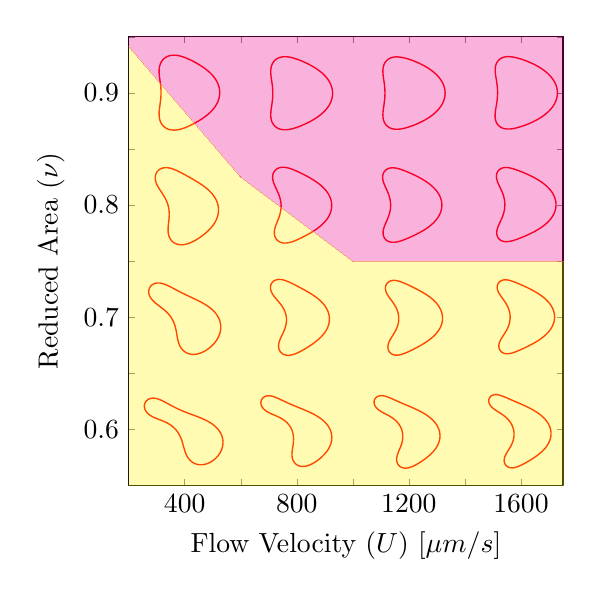
\begin{tikzpicture}[scale=1.0]

\pgfmathsetlengthmacro\MajorTickLength{
      \pgfkeysvalueof{/pgfplots/major tick length} * 0.5
    }

  \begin{axis}[
    major tick length=\MajorTickLength,
    compat=newest,
    axis equal image,
    xmin = 2,
    xmax = 33,
    ymin = -2,
    ymax = 30,
    xtick = {2,6,10,14,18,22,26,30},
    xticklabels = {,$400$,,$800$,,$1200$,,$1600$},
    xlabel = {Flow Velocity ($U$) [$\mu m/s$]},
    ytick = {2,6,10,14,18,22,26,30},
    yticklabels = {$0.6$,,$0.7$,,$0.8$,,$0.9$,},
    ylabel = {Reduced Area ($\nu$)},
    ylabel near ticks,
%    ylabel shift = {-0.3cm},
  ]

% RA = 0.60,flow rate = 200
\addplot[red,line width=0.5pt] coordinates{
%(2.3676e+00,3.6765e-01)
%(2.3997e+00,3.2822e-01)
%(2.4334e+00,2.8830e-01)
%(2.4696e+00,2.4708e-01)
%(2.5092e+00,2.0396e-01)
%(2.5531e+00,1.5862e-01)
%(2.6019e+00,1.1101e-01)
%(2.6566e+00,6.1345e-02)
%(2.7178e+00,1.0104e-02)
%(2.7861e+00,-4.1964e-02)
%(2.8623e+00,-9.3851e-02)
%(2.9469e+00,-1.4429e-01)
%(3.0402e+00,-1.9175e-01)
%(3.1425e+00,-2.3450e-01)
%(3.2536e+00,-2.7064e-01)
%(3.3733e+00,-2.9813e-01)
%(3.5006e+00,-3.1496e-01)
%(3.6345e+00,-3.1918e-01)
%(3.7733e+00,-3.0904e-01)
%(3.9151e+00,-2.8306e-01)
%(4.0576e+00,-2.4008e-01)
%(4.1983e+00,-1.7935e-01)
%(4.3344e+00,-1.0048e-01)
%(4.4630e+00,-3.5203e-03)
%(4.5811e+00,1.1103e-01)
%(4.6853e+00,2.4214e-01)
%(4.7727e+00,3.8824e-01)
%(4.8401e+00,5.4705e-01)
%(4.8850e+00,7.1565e-01)
%(4.9055e+00,8.9050e-01)
%(4.9004e+00,1.0677e+00)
%(4.8699e+00,1.2430e+00)
%(4.8151e+00,1.4129e+00)
%(4.7382e+00,1.5739e+00)
%(4.6419e+00,1.7236e+00)
%(4.5295e+00,1.8608e+00)
%(4.4044e+00,1.9848e+00)
%(4.2696e+00,2.0957e+00)
%(4.1281e+00,2.1945e+00)
%(3.9821e+00,2.2823e+00)
%(3.8338e+00,2.3604e+00)
%(3.6848e+00,2.4303e+00)
%(3.5366e+00,2.4935e+00)
%(3.3901e+00,2.5511e+00)
%(3.2463e+00,2.6044e+00)
%(3.1061e+00,2.6544e+00)
%(2.9699e+00,2.7018e+00)
%(2.8383e+00,2.7473e+00)
%(2.7118e+00,2.7914e+00)
%(2.5906e+00,2.8344e+00)
%(2.4752e+00,2.8764e+00)
%(2.3658e+00,2.9175e+00)
%(2.2624e+00,2.9576e+00)
%(2.1653e+00,2.9968e+00)
%(2.0745e+00,3.0348e+00)
%(1.9899e+00,3.0714e+00)
%(1.9115e+00,3.1066e+00)
%(1.8391e+00,3.1401e+00)
%(1.7725e+00,3.1720e+00)
%(1.7112e+00,3.2020e+00)
%(1.6549e+00,3.2303e+00)
%(1.6028e+00,3.2571e+00)
%(1.5543e+00,3.2826e+00)
%(1.5082e+00,3.3073e+00)
%(1.4635e+00,3.3316e+00)
%(1.4190e+00,3.3562e+00)
%(1.3735e+00,3.3819e+00)
%(1.3259e+00,3.4091e+00)
%(1.2753e+00,3.4385e+00)
%(1.2210e+00,3.4706e+00)
%(1.1625e+00,3.5056e+00)
%(1.0994e+00,3.5440e+00)
%(1.0314e+00,3.5859e+00)
%(9.5848e-01,3.6313e+00)
%(8.8034e-01,3.6801e+00)
%(7.9686e-01,3.7323e+00)
%(7.0785e-01,3.7875e+00)
%(6.1307e-01,3.8450e+00)
%(5.1214e-01,3.9040e+00)
%(4.0459e-01,3.9633e+00)
%(2.8985e-01,4.0211e+00)
%(1.6729e-01,4.0752e+00)
%(3.6375e-02,4.1225e+00)
%(-1.0307e-01,4.1590e+00)
%(-2.5041e-01,4.1798e+00)
%(-4.0355e-01,4.1793e+00)
%(-5.5821e-01,4.1513e+00)
%(-7.0730e-01,4.0910e+00)
%(-8.4111e-01,3.9959e+00)
%(-9.4859e-01,3.8679e+00)
%(-1.0198e+00,3.7137e+00)
%(-1.0483e+00,3.5439e+00)
%(-1.0330e+00,3.3704e+00)
%(-9.7746e-01,3.2035e+00)
%(-8.8809e-01,3.0506e+00)
%(-7.7255e-01,2.9152e+00)
%(-6.3810e-01,2.7979e+00)
%(-4.9085e-01,2.6970e+00)
%(-3.3557e-01,2.6097e+00)
%(-1.7586e-01,2.5325e+00)
%(-1.4370e-02,2.4621e+00)
%(1.4688e-01,2.3950e+00)
%(3.0626e-01,2.3286e+00)
%(4.6240e-01,2.2604e+00)
%(6.1404e-01,2.1890e+00)
%(7.6005e-01,2.1131e+00)
%(8.9944e-01,2.0322e+00)
%(1.0314e+00,1.9464e+00)
%(1.1553e+00,1.8561e+00)
%(1.2708e+00,1.7621e+00)
%(1.3777e+00,1.6654e+00)
%(1.4763e+00,1.5671e+00)
%(1.5670e+00,1.4684e+00)
%(1.6501e+00,1.3704e+00)
%(1.7264e+00,1.2742e+00)
%(1.7965e+00,1.1806e+00)
%(1.8611e+00,1.0905e+00)
%(1.9208e+00,1.0044e+00)
%(1.9761e+00,9.2296e-01)
%(2.0275e+00,8.4642e-01)
%(2.0753e+00,7.7503e-01)
%(2.1200e+00,7.0886e-01)
%(2.1616e+00,6.4786e-01)
%(2.2005e+00,5.9182e-01)
%(2.2370e+00,5.4038e-01)
%(2.2714e+00,4.9302e-01)
%(2.3042e+00,4.4904e-01)
%(2.3360e+00,4.0758e-01)
%(2.3676e+00,3.6765e-01)
};

% RA = 0.65,flow rate = 200
\addplot[red,line width=0.5pt] coordinates{
%(4.6365e+00,5.5272e+00)
%(4.6104e+00,5.5780e+00)
%(4.5819e+00,5.6286e+00)
%(4.5503e+00,5.6800e+00)
%(4.5150e+00,5.7325e+00)
%(4.4753e+00,5.7867e+00)
%(4.4307e+00,5.8427e+00)
%(4.3806e+00,5.9004e+00)
%(4.3245e+00,5.9596e+00)
%(4.2618e+00,6.0201e+00)
%(4.1924e+00,6.0815e+00)
%(4.1160e+00,6.1434e+00)
%(4.0325e+00,6.2053e+00)
%(3.9418e+00,6.2669e+00)
%(3.8441e+00,6.3278e+00)
%(3.7396e+00,6.3879e+00)
%(3.6285e+00,6.4469e+00)
%(3.5112e+00,6.5048e+00)
%(3.3880e+00,6.5618e+00)
%(3.2595e+00,6.6181e+00)
%(3.1260e+00,6.6740e+00)
%(2.9882e+00,6.7300e+00)
%(2.8465e+00,6.7866e+00)
%(2.7015e+00,6.8444e+00)
%(2.5538e+00,6.9038e+00)
%(2.4039e+00,6.9656e+00)
%(2.2524e+00,7.0302e+00)
%(2.1001e+00,7.0981e+00)
%(1.9473e+00,7.1696e+00)
%(1.7948e+00,7.2448e+00)
%(1.6428e+00,7.3238e+00)
%(1.4919e+00,7.4062e+00)
%(1.3422e+00,7.4916e+00)
%(1.1938e+00,7.5791e+00)
%(1.0465e+00,7.6678e+00)
%(8.9992e-01,7.7563e+00)
%(7.5347e-01,7.8428e+00)
%(6.0643e-01,7.9254e+00)
%(4.5803e-01,8.0016e+00)
%(3.0765e-01,8.0685e+00)
%(1.5503e-01,8.1230e+00)
%(6.2232e-04,8.1617e+00)
%(-1.5412e-01,8.1810e+00)
%(-3.0651e-01,8.1781e+00)
%(-4.5260e-01,8.1511e+00)
%(-5.8754e-01,8.0995e+00)
%(-7.0631e-01,8.0252e+00)
%(-8.0461e-01,7.9319e+00)
%(-8.7974e-01,7.8251e+00)
%(-9.3092e-01,7.7103e+00)
%(-9.5928e-01,7.5933e+00)
%(-9.6737e-01,7.4786e+00)
%(-9.5850e-01,7.3694e+00)
%(-9.3625e-01,7.2679e+00)
%(-9.0401e-01,7.1751e+00)
%(-8.6478e-01,7.0911e+00)
%(-8.2104e-01,7.0158e+00)
%(-7.7475e-01,6.9486e+00)
%(-7.2739e-01,6.8886e+00)
%(-6.7997e-01,6.8350e+00)
%(-6.3313e-01,6.7869e+00)
%(-5.8712e-01,6.7434e+00)
%(-5.4188e-01,6.7036e+00)
%(-4.9708e-01,6.6665e+00)
%(-4.5216e-01,6.6313e+00)
%(-4.0640e-01,6.5972e+00)
%(-3.5900e-01,6.5635e+00)
%(-3.0919e-01,6.5296e+00)
%(-2.5622e-01,6.4949e+00)
%(-1.9949e-01,6.4589e+00)
%(-1.3852e-01,6.4215e+00)
%(-7.2943e-02,6.3822e+00)
%(-2.5571e-03,6.3408e+00)
%(7.2727e-02,6.2970e+00)
%(1.5287e-01,6.2505e+00)
%(2.3772e-01,6.2008e+00)
%(3.2699e-01,6.1475e+00)
%(4.2029e-01,6.0899e+00)
%(5.1714e-01,6.0277e+00)
%(6.1690e-01,5.9600e+00)
%(7.1889e-01,5.8863e+00)
%(8.2232e-01,5.8062e+00)
%(9.2637e-01,5.7191e+00)
%(1.0302e+00,5.6247e+00)
%(1.1331e+00,5.5230e+00)
%(1.2344e+00,5.4141e+00)
%(1.3338e+00,5.2982e+00)
%(1.4309e+00,5.1761e+00)
%(1.5261e+00,5.0484e+00)
%(1.6200e+00,4.9162e+00)
%(1.7134e+00,4.7806e+00)
%(1.8077e+00,4.6430e+00)
%(1.9045e+00,4.5049e+00)
%(2.0055e+00,4.3681e+00)
%(2.1127e+00,4.2345e+00)
%(2.2276e+00,4.1067e+00)
%(2.3515e+00,3.9869e+00)
%(2.4851e+00,3.8781e+00)
%(2.6282e+00,3.7828e+00)
%(2.7799e+00,3.7036e+00)
%(2.9385e+00,3.6424e+00)
%(3.1018e+00,3.6006e+00)
%(3.2671e+00,3.5787e+00)
%(3.4316e+00,3.5766e+00)
%(3.5928e+00,3.5934e+00)
%(3.7483e+00,3.6277e+00)
%(3.8960e+00,3.6779e+00)
%(4.0343e+00,3.7421e+00)
%(4.1620e+00,3.8185e+00)
%(4.2779e+00,3.9049e+00)
%(4.3816e+00,3.9994e+00)
%(4.4725e+00,4.1001e+00)
%(4.5505e+00,4.2052e+00)
%(4.6157e+00,4.3127e+00)
%(4.6685e+00,4.4210e+00)
%(4.7096e+00,4.5285e+00)
%(4.7399e+00,4.6339e+00)
%(4.7602e+00,4.7358e+00)
%(4.7718e+00,4.8335e+00)
%(4.7759e+00,4.9260e+00)
%(4.7737e+00,5.0131e+00)
%(4.7663e+00,5.0944e+00)
%(4.7548e+00,5.1699e+00)
%(4.7401e+00,5.2399e+00)
%(4.7228e+00,5.3048e+00)
%(4.7037e+00,5.3652e+00)
%(4.6829e+00,5.4218e+00)
%(4.6605e+00,5.4755e+00)
%(4.6365e+00,5.5272e+00)
};

% RA = 0.70,flow rate = 200
\addplot[red,line width=0.5pt] coordinates{
%(2.7354e+00,1.0999e+01)
%(2.6782e+00,1.1024e+01)
%(2.6202e+00,1.1050e+01)
%(2.5606e+00,1.1076e+01)
%(2.4986e+00,1.1104e+01)
%(2.4336e+00,1.1133e+01)
%(2.3652e+00,1.1164e+01)
%(2.2930e+00,1.1198e+01)
%(2.2167e+00,1.1233e+01)
%(2.1362e+00,1.1272e+01)
%(2.0513e+00,1.1313e+01)
%(1.9622e+00,1.1358e+01)
%(1.8689e+00,1.1405e+01)
%(1.7714e+00,1.1456e+01)
%(1.6699e+00,1.1511e+01)
%(1.5646e+00,1.1569e+01)
%(1.4555e+00,1.1631e+01)
%(1.3428e+00,1.1696e+01)
%(1.2266e+00,1.1764e+01)
%(1.1066e+00,1.1834e+01)
%(9.8286e-01,1.1906e+01)
%(8.5490e-01,1.1978e+01)
%(7.2224e-01,1.2049e+01)
%(5.8426e-01,1.2118e+01)
%(4.4027e-01,1.2180e+01)
%(2.8977e-01,1.2233e+01)
%(1.3273e-01,1.2273e+01)
%(-2.9927e-02,1.2294e+01)
%(-1.9563e-01,1.2292e+01)
%(-3.5964e-01,1.2260e+01)
%(-5.1479e-01,1.2195e+01)
%(-6.5210e-01,1.2097e+01)
%(-7.6239e-01,1.1969e+01)
%(-8.3835e-01,1.1818e+01)
%(-8.7638e-01,1.1654e+01)
%(-8.7699e-01,1.1486e+01)
%(-8.4408e-01,1.1322e+01)
%(-7.8341e-01,1.1168e+01)
%(-7.0131e-01,1.1026e+01)
%(-6.0364e-01,1.0897e+01)
%(-4.9541e-01,1.0779e+01)
%(-3.8067e-01,1.0672e+01)
%(-2.6258e-01,1.0573e+01)
%(-1.4356e-01,1.0481e+01)
%(-2.5489e-02,1.0393e+01)
%(9.0185e-02,1.0309e+01)
%(2.0234e-01,1.0227e+01)
%(3.1013e-01,1.0146e+01)
%(4.1289e-01,1.0067e+01)
%(5.1018e-01,9.9877e+00)
%(6.0169e-01,9.9096e+00)
%(6.8730e-01,9.8324e+00)
%(7.6698e-01,9.7564e+00)
%(8.4085e-01,9.6820e+00)
%(9.0911e-01,9.6095e+00)
%(9.7203e-01,9.5392e+00)
%(1.0300e+00,9.4713e+00)
%(1.0833e+00,9.4061e+00)
%(1.1324e+00,9.3435e+00)
%(1.1779e+00,9.2836e+00)
%(1.2201e+00,9.2262e+00)
%(1.2596e+00,9.1710e+00)
%(1.2969e+00,9.1175e+00)
%(1.3327e+00,9.0652e+00)
%(1.3676e+00,9.0133e+00)
%(1.4020e+00,8.9612e+00)
%(1.4368e+00,8.9082e+00)
%(1.4723e+00,8.8535e+00)
%(1.5091e+00,8.7964e+00)
%(1.5477e+00,8.7365e+00)
%(1.5886e+00,8.6734e+00)
%(1.6321e+00,8.6069e+00)
%(1.6788e+00,8.5367e+00)
%(1.7292e+00,8.4631e+00)
%(1.7837e+00,8.3861e+00)
%(1.8431e+00,8.3061e+00)
%(1.9080e+00,8.2238e+00)
%(1.9792e+00,8.1398e+00)
%(2.0576e+00,8.0553e+00)
%(2.1438e+00,7.9714e+00)
%(2.2388e+00,7.8898e+00)
%(2.3430e+00,7.8120e+00)
%(2.4568e+00,7.7402e+00)
%(2.5802e+00,7.6763e+00)
%(2.7128e+00,7.6226e+00)
%(2.8538e+00,7.5810e+00)
%(3.0018e+00,7.5534e+00)
%(3.1552e+00,7.5412e+00)
%(3.3120e+00,7.5453e+00)
%(3.4702e+00,7.5664e+00)
%(3.6277e+00,7.6046e+00)
%(3.7823e+00,7.6597e+00)
%(3.9318e+00,7.7314e+00)
%(4.0744e+00,7.8189e+00)
%(4.2078e+00,7.9215e+00)
%(4.3302e+00,8.0380e+00)
%(4.4396e+00,8.1673e+00)
%(4.5340e+00,8.3079e+00)
%(4.6116e+00,8.4580e+00)
%(4.6709e+00,8.6155e+00)
%(4.7107e+00,8.7779e+00)
%(4.7306e+00,8.9426e+00)
%(4.7305e+00,9.1067e+00)
%(4.7112e+00,9.2675e+00)
%(4.6741e+00,9.4228e+00)
%(4.6210e+00,9.5705e+00)
%(4.5543e+00,9.7092e+00)
%(4.4763e+00,9.8380e+00)
%(4.3894e+00,9.9565e+00)
%(4.2960e+00,1.0065e+01)
%(4.1980e+00,1.0163e+01)
%(4.0973e+00,1.0253e+01)
%(3.9955e+00,1.0334e+01)
%(3.8939e+00,1.0407e+01)
%(3.7935e+00,1.0473e+01)
%(3.6953e+00,1.0534e+01)
%(3.5998e+00,1.0589e+01)
%(3.5077e+00,1.0639e+01)
%(3.4193e+00,1.0684e+01)
%(3.3348e+00,1.0726e+01)
%(3.2544e+00,1.0765e+01)
%(3.1781e+00,1.0801e+01)
%(3.1059e+00,1.0834e+01)
%(3.0374e+00,1.0865e+01)
%(2.9724e+00,1.0894e+01)
%(2.9103e+00,1.0922e+01)
%(2.8506e+00,1.0948e+01)
%(2.7926e+00,1.0974e+01)
%(2.7354e+00,1.0999e+01)
};

% RA = 0.75,flow rate = 200
\addplot[red,line width=0.5pt] coordinates{
%(1.3501e+00,1.5934e+01)
%(1.2911e+00,1.5968e+01)
%(1.2312e+00,1.6002e+01)
%(1.1699e+00,1.6036e+01)
%(1.1063e+00,1.6071e+01)
%(1.0399e+00,1.6107e+01)
%(9.7001e-01,1.6144e+01)
%(8.9614e-01,1.6182e+01)
%(8.1776e-01,1.6220e+01)
%(7.3440e-01,1.6259e+01)
%(6.4559e-01,1.6296e+01)
%(5.5092e-01,1.6332e+01)
%(4.5001e-01,1.6365e+01)
%(3.4263e-01,1.6392e+01)
%(2.2878e-01,1.6413e+01)
%(1.0884e-01,1.6424e+01)
%(-1.6164e-02,1.6422e+01)
%(-1.4430e-01,1.6403e+01)
%(-2.7244e-01,1.6365e+01)
%(-3.9616e-01,1.6304e+01)
%(-5.0986e-01,1.6219e+01)
%(-6.0731e-01,1.6112e+01)
%(-6.8259e-01,1.5983e+01)
%(-7.3114e-01,1.5839e+01)
%(-7.5058e-01,1.5686e+01)
%(-7.4090e-01,1.5529e+01)
%(-7.0418e-01,1.5373e+01)
%(-6.4387e-01,1.5223e+01)
%(-5.6407e-01,1.5081e+01)
%(-4.6894e-01,1.4946e+01)
%(-3.6230e-01,1.4819e+01)
%(-2.4752e-01,1.4699e+01)
%(-1.2747e-01,1.4583e+01)
%(-4.5946e-03,1.4470e+01)
%(1.1906e-01,1.4358e+01)
%(2.4175e-01,1.4247e+01)
%(3.6196e-01,1.4134e+01)
%(4.7846e-01,1.4019e+01)
%(5.9026e-01,1.3902e+01)
%(6.9661e-01,1.3783e+01)
%(7.9707e-01,1.3662e+01)
%(8.9146e-01,1.3539e+01)
%(9.7990e-01,1.3415e+01)
%(1.0627e+00,1.3291e+01)
%(1.1405e+00,1.3168e+01)
%(1.2140e+00,1.3047e+01)
%(1.2839e+00,1.2928e+01)
%(1.3511e+00,1.2812e+01)
%(1.4163e+00,1.2700e+01)
%(1.4802e+00,1.2592e+01)
%(1.5434e+00,1.2490e+01)
%(1.6063e+00,1.2392e+01)
%(1.6692e+00,1.2301e+01)
%(1.7321e+00,1.2216e+01)
%(1.7951e+00,1.2136e+01)
%(1.8581e+00,1.2063e+01)
%(1.9210e+00,1.1997e+01)
%(1.9835e+00,1.1936e+01)
%(2.0454e+00,1.1881e+01)
%(2.1068e+00,1.1831e+01)
%(2.1675e+00,1.1786e+01)
%(2.2278e+00,1.1745e+01)
%(2.2879e+00,1.1708e+01)
%(2.3481e+00,1.1675e+01)
%(2.4090e+00,1.1645e+01)
%(2.4712e+00,1.1618e+01)
%(2.5354e+00,1.1593e+01)
%(2.6022e+00,1.1571e+01)
%(2.6722e+00,1.1552e+01)
%(2.7459e+00,1.1535e+01)
%(2.8239e+00,1.1522e+01)
%(2.9063e+00,1.1512e+01)
%(2.9934e+00,1.1508e+01)
%(3.0852e+00,1.1508e+01)
%(3.1814e+00,1.1514e+01)
%(3.2818e+00,1.1526e+01)
%(3.3860e+00,1.1546e+01)
%(3.4933e+00,1.1574e+01)
%(3.6031e+00,1.1611e+01)
%(3.7145e+00,1.1657e+01)
%(3.8266e+00,1.1712e+01)
%(3.9384e+00,1.1778e+01)
%(4.0486e+00,1.1854e+01)
%(4.1561e+00,1.1940e+01)
%(4.2594e+00,1.2038e+01)
%(4.3569e+00,1.2146e+01)
%(4.4469e+00,1.2264e+01)
%(4.5276e+00,1.2393e+01)
%(4.5971e+00,1.2532e+01)
%(4.6533e+00,1.2679e+01)
%(4.6944e+00,1.2833e+01)
%(4.7189e+00,1.2993e+01)
%(4.7256e+00,1.3156e+01)
%(4.7137e+00,1.3321e+01)
%(4.6832e+00,1.3484e+01)
%(4.6347e+00,1.3643e+01)
%(4.5693e+00,1.3796e+01)
%(4.4886e+00,1.3942e+01)
%(4.3947e+00,1.4080e+01)
%(4.2897e+00,1.4208e+01)
%(4.1755e+00,1.4327e+01)
%(4.0544e+00,1.4436e+01)
%(3.9281e+00,1.4538e+01)
%(3.7983e+00,1.4631e+01)
%(3.6664e+00,1.4717e+01)
%(3.5336e+00,1.4797e+01)
%(3.4011e+00,1.4872e+01)
%(3.2696e+00,1.4942e+01)
%(3.1401e+00,1.5008e+01)
%(3.0130e+00,1.5072e+01)
%(2.8889e+00,1.5132e+01)
%(2.7683e+00,1.5190e+01)
%(2.6516e+00,1.5246e+01)
%(2.5390e+00,1.5301e+01)
%(2.4307e+00,1.5354e+01)
%(2.3269e+00,1.5405e+01)
%(2.2278e+00,1.5455e+01)
%(2.1334e+00,1.5503e+01)
%(2.0435e+00,1.5550e+01)
%(1.9583e+00,1.5595e+01)
%(1.8774e+00,1.5638e+01)
%(1.8008e+00,1.5680e+01)
%(1.7282e+00,1.5720e+01)
%(1.6591e+00,1.5759e+01)
%(1.5932e+00,1.5796e+01)
%(1.5300e+00,1.5832e+01)
%(1.4688e+00,1.5866e+01)
%(1.4091e+00,1.5900e+01)
%(1.3501e+00,1.5934e+01)
};

% RA = 0.80,flow rate = 200
\addplot[red,line width=0.5pt] coordinates{
%(-5.6959e-03,2.0451e+01)
%(-7.7009e-02,2.0432e+01)
%(-1.4714e-01,2.0407e+01)
%(-2.1601e-01,2.0375e+01)
%(-2.8329e-01,2.0336e+01)
%(-3.4837e-01,2.0289e+01)
%(-4.1033e-01,2.0233e+01)
%(-4.6795e-01,2.0168e+01)
%(-5.1972e-01,2.0094e+01)
%(-5.6397e-01,2.0011e+01)
%(-5.9898e-01,1.9918e+01)
%(-6.2315e-01,1.9818e+01)
%(-6.3512e-01,1.9711e+01)
%(-6.3392e-01,1.9599e+01)
%(-6.1909e-01,1.9484e+01)
%(-5.9064e-01,1.9367e+01)
%(-5.4906e-01,1.9249e+01)
%(-4.9524e-01,1.9132e+01)
%(-4.3036e-01,1.9016e+01)
%(-3.5578e-01,1.8901e+01)
%(-2.7297e-01,1.8788e+01)
%(-1.8345e-01,1.8675e+01)
%(-8.8729e-02,1.8562e+01)
%(9.7143e-03,1.8449e+01)
%(1.1044e-01,1.8334e+01)
%(2.1207e-01,1.8217e+01)
%(3.1330e-01,1.8097e+01)
%(4.1293e-01,1.7973e+01)
%(5.0994e-01,1.7845e+01)
%(6.0346e-01,1.7713e+01)
%(6.9292e-01,1.7577e+01)
%(7.7805e-01,1.7437e+01)
%(8.5889e-01,1.7295e+01)
%(9.3588e-01,1.7150e+01)
%(1.0098e+00,1.7005e+01)
%(1.0816e+00,1.6859e+01)
%(1.1528e+00,1.6713e+01)
%(1.2246e+00,1.6570e+01)
%(1.2988e+00,1.6429e+01)
%(1.3766e+00,1.6292e+01)
%(1.4594e+00,1.6161e+01)
%(1.5481e+00,1.6037e+01)
%(1.6432e+00,1.5921e+01)
%(1.7449e+00,1.5815e+01)
%(1.8526e+00,1.5719e+01)
%(1.9655e+00,1.5636e+01)
%(2.0824e+00,1.5565e+01)
%(2.2018e+00,1.5506e+01)
%(2.3224e+00,1.5460e+01)
%(2.4426e+00,1.5426e+01)
%(2.5610e+00,1.5403e+01)
%(2.6765e+00,1.5390e+01)
%(2.7884e+00,1.5386e+01)
%(2.8958e+00,1.5390e+01)
%(2.9984e+00,1.5400e+01)
%(3.0960e+00,1.5415e+01)
%(3.1884e+00,1.5435e+01)
%(3.2758e+00,1.5459e+01)
%(3.3585e+00,1.5486e+01)
%(3.4366e+00,1.5515e+01)
%(3.5107e+00,1.5546e+01)
%(3.5811e+00,1.5579e+01)
%(3.6485e+00,1.5614e+01)
%(3.7135e+00,1.5651e+01)
%(3.7764e+00,1.5689e+01)
%(3.8380e+00,1.5730e+01)
%(3.8987e+00,1.5773e+01)
%(3.9588e+00,1.5819e+01)
%(4.0188e+00,1.5869e+01)
%(4.0787e+00,1.5923e+01)
%(4.1386e+00,1.5981e+01)
%(4.1984e+00,1.6044e+01)
%(4.2578e+00,1.6112e+01)
%(4.3165e+00,1.6186e+01)
%(4.3737e+00,1.6267e+01)
%(4.4288e+00,1.6354e+01)
%(4.4809e+00,1.6448e+01)
%(4.5289e+00,1.6549e+01)
%(4.5717e+00,1.6657e+01)
%(4.6080e+00,1.6772e+01)
%(4.6364e+00,1.6894e+01)
%(4.6557e+00,1.7021e+01)
%(4.6643e+00,1.7154e+01)
%(4.6613e+00,1.7291e+01)
%(4.6456e+00,1.7430e+01)
%(4.6165e+00,1.7571e+01)
%(4.5738e+00,1.7712e+01)
%(4.5174e+00,1.7851e+01)
%(4.4479e+00,1.7987e+01)
%(4.3658e+00,1.8118e+01)
%(4.2723e+00,1.8245e+01)
%(4.1686e+00,1.8365e+01)
%(4.0558e+00,1.8480e+01)
%(3.9354e+00,1.8588e+01)
%(3.8087e+00,1.8690e+01)
%(3.6769e+00,1.8786e+01)
%(3.5411e+00,1.8878e+01)
%(3.4024e+00,1.8965e+01)
%(3.2618e+00,1.9048e+01)
%(3.1201e+00,1.9128e+01)
%(2.9781e+00,1.9206e+01)
%(2.8364e+00,1.9282e+01)
%(2.6958e+00,1.9356e+01)
%(2.5566e+00,1.9429e+01)
%(2.4195e+00,1.9502e+01)
%(2.2847e+00,1.9574e+01)
%(2.1526e+00,1.9645e+01)
%(2.0235e+00,1.9715e+01)
%(1.8975e+00,1.9785e+01)
%(1.7748e+00,1.9853e+01)
%(1.6554e+00,1.9920e+01)
%(1.5394e+00,1.9985e+01)
%(1.4265e+00,2.0047e+01)
%(1.3168e+00,2.0107e+01)
%(1.2102e+00,2.0164e+01)
%(1.1065e+00,2.0216e+01)
%(1.0057e+00,2.0265e+01)
%(9.0761e-01,2.0309e+01)
%(8.1223e-01,2.0348e+01)
%(7.1950e-01,2.0382e+01)
%(6.2940e-01,2.0411e+01)
%(5.4191e-01,2.0434e+01)
%(4.5700e-01,2.0452e+01)
%(3.7459e-01,2.0465e+01)
%(2.9457e-01,2.0473e+01)
%(2.1677e-01,2.0475e+01)
%(1.4096e-01,2.0472e+01)
%(6.6893e-02,2.0465e+01)
%(-5.6959e-03,2.0451e+01)
};

% RA = 0.85,flow rate = 200
\addplot[red,line width=0.5pt] coordinates{
%(1.1897e+00,2.4414e+01)
%(1.1157e+00,2.4445e+01)
%(1.0404e+00,2.4475e+01)
%(9.6319e-01,2.4502e+01)
%(8.8353e-01,2.4528e+01)
%(8.0087e-01,2.4550e+01)
%(7.1478e-01,2.4570e+01)
%(6.2490e-01,2.4585e+01)
%(5.3105e-01,2.4595e+01)
%(4.3326e-01,2.4599e+01)
%(3.3189e-01,2.4594e+01)
%(2.2766e-01,2.4580e+01)
%(1.2184e-01,2.4553e+01)
%(1.6274e-02,2.4513e+01)
%(-8.6567e-02,2.4457e+01)
%(-1.8363e-01,2.4385e+01)
%(-2.7148e-01,2.4297e+01)
%(-3.4665e-01,2.4193e+01)
%(-4.0601e-01,2.4075e+01)
%(-4.4721e-01,2.3946e+01)
%(-4.6896e-01,2.3809e+01)
%(-4.7110e-01,2.3668e+01)
%(-4.5452e-01,2.3524e+01)
%(-4.2094e-01,2.3381e+01)
%(-3.7257e-01,2.3239e+01)
%(-3.1188e-01,2.3099e+01)
%(-2.4139e-01,2.2962e+01)
%(-1.6352e-01,2.2828e+01)
%(-8.0514e-02,2.2694e+01)
%(5.5560e-03,2.2561e+01)
%(9.2846e-02,2.2428e+01)
%(1.7972e-01,2.2294e+01)
%(2.6478e-01,2.2159e+01)
%(3.4685e-01,2.2021e+01)
%(4.2506e-01,2.1882e+01)
%(4.9880e-01,2.1741e+01)
%(5.6780e-01,2.1599e+01)
%(6.3210e-01,2.1455e+01)
%(6.9205e-01,2.1312e+01)
%(7.4829e-01,2.1168e+01)
%(8.0169e-01,2.1026e+01)
%(8.5331e-01,2.0885e+01)
%(9.0431e-01,2.0747e+01)
%(9.5586e-01,2.0612e+01)
%(1.0091e+00,2.0480e+01)
%(1.0651e+00,2.0353e+01)
%(1.1247e+00,2.0232e+01)
%(1.1885e+00,2.0116e+01)
%(1.2568e+00,2.0007e+01)
%(1.3296e+00,1.9906e+01)
%(1.4068e+00,1.9813e+01)
%(1.4877e+00,1.9729e+01)
%(1.5719e+00,1.9653e+01)
%(1.6584e+00,1.9587e+01)
%(1.7465e+00,1.9529e+01)
%(1.8354e+00,1.9480e+01)
%(1.9243e+00,1.9439e+01)
%(2.0126e+00,1.9405e+01)
%(2.0998e+00,1.9379e+01)
%(2.1858e+00,1.9359e+01)
%(2.2703e+00,1.9344e+01)
%(2.3534e+00,1.9335e+01)
%(2.4353e+00,1.9330e+01)
%(2.5161e+00,1.9330e+01)
%(2.5963e+00,1.9333e+01)
%(2.6763e+00,1.9341e+01)
%(2.7563e+00,1.9352e+01)
%(2.8369e+00,1.9367e+01)
%(2.9183e+00,1.9386e+01)
%(3.0009e+00,1.9410e+01)
%(3.0849e+00,1.9437e+01)
%(3.1703e+00,1.9469e+01)
%(3.2573e+00,1.9506e+01)
%(3.3458e+00,1.9547e+01)
%(3.4356e+00,1.9595e+01)
%(3.5267e+00,1.9648e+01)
%(3.6187e+00,1.9706e+01)
%(3.7112e+00,1.9771e+01)
%(3.8038e+00,1.9843e+01)
%(3.8959e+00,1.9921e+01)
%(3.9868e+00,2.0007e+01)
%(4.0757e+00,2.0099e+01)
%(4.1617e+00,2.0199e+01)
%(4.2438e+00,2.0307e+01)
%(4.3207e+00,2.0423e+01)
%(4.3910e+00,2.0546e+01)
%(4.4534e+00,2.0676e+01)
%(4.5064e+00,2.0814e+01)
%(4.5484e+00,2.0958e+01)
%(4.5781e+00,2.1107e+01)
%(4.5942e+00,2.1260e+01)
%(4.5959e+00,2.1416e+01)
%(4.5825e+00,2.1572e+01)
%(4.5539e+00,2.1728e+01)
%(4.5105e+00,2.1881e+01)
%(4.4531e+00,2.2030e+01)
%(4.3826e+00,2.2173e+01)
%(4.3005e+00,2.2311e+01)
%(4.2083e+00,2.2441e+01)
%(4.1076e+00,2.2564e+01)
%(3.9998e+00,2.2680e+01)
%(3.8866e+00,2.2789e+01)
%(3.7692e+00,2.2891e+01)
%(3.6490e+00,2.2988e+01)
%(3.5269e+00,2.3078e+01)
%(3.4040e+00,2.3164e+01)
%(3.2811e+00,2.3245e+01)
%(3.1589e+00,2.3323e+01)
%(3.0379e+00,2.3397e+01)
%(2.9188e+00,2.3468e+01)
%(2.8019e+00,2.3536e+01)
%(2.6876e+00,2.3602e+01)
%(2.5761e+00,2.3666e+01)
%(2.4677e+00,2.3728e+01)
%(2.3626e+00,2.3788e+01)
%(2.2608e+00,2.3845e+01)
%(2.1624e+00,2.3901e+01)
%(2.0673e+00,2.3955e+01)
%(1.9756e+00,2.4006e+01)
%(1.8870e+00,2.4056e+01)
%(1.8015e+00,2.4104e+01)
%(1.7187e+00,2.4149e+01)
%(1.6386e+00,2.4193e+01)
%(1.5606e+00,2.4234e+01)
%(1.4845e+00,2.4274e+01)
%(1.4099e+00,2.4311e+01)
%(1.3362e+00,2.4347e+01)
%(1.2630e+00,2.4382e+01)
%(1.1897e+00,2.4414e+01)
};

% RA = 0.90,flow rate = 200
\addplot[red,line width=0.5pt] coordinates{
%(3.8381e+00,2.4242e+01)
%(3.8983e+00,2.4309e+01)
%(3.9567e+00,2.4378e+01)
%(4.0134e+00,2.4449e+01)
%(4.0682e+00,2.4523e+01)
%(4.1211e+00,2.4600e+01)
%(4.1719e+00,2.4681e+01)
%(4.2204e+00,2.4766e+01)
%(4.2661e+00,2.4855e+01)
%(4.3085e+00,2.4948e+01)
%(4.3471e+00,2.5046e+01)
%(4.3812e+00,2.5148e+01)
%(4.4100e+00,2.5256e+01)
%(4.4328e+00,2.5367e+01)
%(4.4488e+00,2.5483e+01)
%(4.4571e+00,2.5603e+01)
%(4.4570e+00,2.5726e+01)
%(4.4478e+00,2.5851e+01)
%(4.4291e+00,2.5979e+01)
%(4.4005e+00,2.6107e+01)
%(4.3617e+00,2.6236e+01)
%(4.3129e+00,2.6363e+01)
%(4.2543e+00,2.6490e+01)
%(4.1863e+00,2.6613e+01)
%(4.1094e+00,2.6734e+01)
%(4.0244e+00,2.6852e+01)
%(3.9320e+00,2.6965e+01)
%(3.8329e+00,2.7075e+01)
%(3.7281e+00,2.7181e+01)
%(3.6184e+00,2.7284e+01)
%(3.5044e+00,2.7382e+01)
%(3.3870e+00,2.7478e+01)
%(3.2668e+00,2.7570e+01)
%(3.1444e+00,2.7659e+01)
%(3.0204e+00,2.7746e+01)
%(2.8953e+00,2.7830e+01)
%(2.7694e+00,2.7911e+01)
%(2.6431e+00,2.7991e+01)
%(2.5168e+00,2.8068e+01)
%(2.3905e+00,2.8142e+01)
%(2.2644e+00,2.8214e+01)
%(2.1388e+00,2.8282e+01)
%(2.0135e+00,2.8347e+01)
%(1.8886e+00,2.8408e+01)
%(1.7641e+00,2.8465e+01)
%(1.6400e+00,2.8516e+01)
%(1.5164e+00,2.8561e+01)
%(1.3935e+00,2.8599e+01)
%(1.2713e+00,2.8630e+01)
%(1.1504e+00,2.8653e+01)
%(1.0312e+00,2.8666e+01)
%(9.1431e-01,2.8670e+01)
%(8.0052e-01,2.8665e+01)
%(6.9066e-01,2.8649e+01)
%(5.8565e-01,2.8624e+01)
%(4.8635e-01,2.8590e+01)
%(3.9356e-01,2.8546e+01)
%(3.0794e-01,2.8495e+01)
%(2.2997e-01,2.8436e+01)
%(1.5996e-01,2.8371e+01)
%(9.8035e-02,2.8301e+01)
%(4.4159e-02,2.8226e+01)
%(-1.8319e-03,2.8148e+01)
%(-4.0189e-02,2.8066e+01)
%(-7.1217e-02,2.7982e+01)
%(-9.5246e-02,2.7896e+01)
%(-1.1261e-01,2.7807e+01)
%(-1.2363e-01,2.7717e+01)
%(-1.2864e-01,2.7625e+01)
%(-1.2792e-01,2.7531e+01)
%(-1.2181e-01,2.7436e+01)
%(-1.1063e-01,2.7339e+01)
%(-9.4729e-02,2.7240e+01)
%(-7.4496e-02,2.7140e+01)
%(-5.0361e-02,2.7037e+01)
%(-2.2803e-02,2.6933e+01)
%(7.6509e-03,2.6826e+01)
%(4.0427e-02,2.6717e+01)
%(7.4910e-02,2.6605e+01)
%(1.1046e-01,2.6490e+01)
%(1.4641e-01,2.6373e+01)
%(1.8211e-01,2.6252e+01)
%(2.1694e-01,2.6128e+01)
%(2.5033e-01,2.6000e+01)
%(2.8184e-01,2.5870e+01)
%(3.1114e-01,2.5736e+01)
%(3.3807e-01,2.5600e+01)
%(3.6269e-01,2.5461e+01)
%(3.8530e-01,2.5320e+01)
%(4.0646e-01,2.5176e+01)
%(4.2702e-01,2.5031e+01)
%(4.4809e-01,2.4884e+01)
%(4.7104e-01,2.4737e+01)
%(4.9749e-01,2.4589e+01)
%(5.2920e-01,2.4442e+01)
%(5.6805e-01,2.4296e+01)
%(6.1587e-01,2.4152e+01)
%(6.7433e-01,2.4012e+01)
%(7.4470e-01,2.3879e+01)
%(8.2775e-01,2.3753e+01)
%(9.2355e-01,2.3638e+01)
%(1.0314e+00,2.3535e+01)
%(1.1499e+00,2.3446e+01)
%(1.2771e+00,2.3373e+01)
%(1.4105e+00,2.3317e+01)
%(1.5479e+00,2.3277e+01)
%(1.6868e+00,2.3252e+01)
%(1.8255e+00,2.3241e+01)
%(1.9621e+00,2.3243e+01)
%(2.0957e+00,2.3256e+01)
%(2.2254e+00,2.3278e+01)
%(2.3507e+00,2.3308e+01)
%(2.4713e+00,2.3345e+01)
%(2.5871e+00,2.3386e+01)
%(2.6981e+00,2.3432e+01)
%(2.8043e+00,2.3481e+01)
%(2.9060e+00,2.3533e+01)
%(3.0032e+00,2.3586e+01)
%(3.0962e+00,2.3641e+01)
%(3.1851e+00,2.3698e+01)
%(3.2702e+00,2.3755e+01)
%(3.3515e+00,2.3813e+01)
%(3.4295e+00,2.3872e+01)
%(3.5042e+00,2.3931e+01)
%(3.5760e+00,2.3991e+01)
%(3.6451e+00,2.4052e+01)
%(3.7116e+00,2.4114e+01)
%(3.7759e+00,2.4178e+01)
%(3.8381e+00,2.4242e+01)
};

% RA = 0.95,flow rate = 200
\addplot[red,line width=0.5pt] coordinates{
%(5.3512e-01,2.7659e+01)
%(6.1155e-01,2.7596e+01)
%(6.9316e-01,2.7540e+01)
%(7.7965e-01,2.7490e+01)
%(8.7067e-01,2.7447e+01)
%(9.6584e-01,2.7411e+01)
%(1.0648e+00,2.7383e+01)
%(1.1670e+00,2.7362e+01)
%(1.2721e+00,2.7348e+01)
%(1.3798e+00,2.7342e+01)
%(1.4895e+00,2.7343e+01)
%(1.6011e+00,2.7351e+01)
%(1.7141e+00,2.7366e+01)
%(1.8282e+00,2.7387e+01)
%(1.9434e+00,2.7415e+01)
%(2.0593e+00,2.7448e+01)
%(2.1759e+00,2.7487e+01)
%(2.2930e+00,2.7531e+01)
%(2.4105e+00,2.7580e+01)
%(2.5283e+00,2.7633e+01)
%(2.6463e+00,2.7691e+01)
%(2.7644e+00,2.7752e+01)
%(2.8823e+00,2.7818e+01)
%(3.0000e+00,2.7888e+01)
%(3.1171e+00,2.7961e+01)
%(3.2334e+00,2.8038e+01)
%(3.3485e+00,2.8119e+01)
%(3.4620e+00,2.8205e+01)
%(3.5733e+00,2.8294e+01)
%(3.6821e+00,2.8388e+01)
%(3.7875e+00,2.8486e+01)
%(3.8890e+00,2.8589e+01)
%(3.9857e+00,2.8696e+01)
%(4.0768e+00,2.8809e+01)
%(4.1615e+00,2.8926e+01)
%(4.2388e+00,2.9047e+01)
%(4.3080e+00,2.9173e+01)
%(4.3682e+00,2.9302e+01)
%(4.4187e+00,2.9435e+01)
%(4.4589e+00,2.9570e+01)
%(4.4884e+00,2.9706e+01)
%(4.5070e+00,2.9843e+01)
%(4.5148e+00,2.9980e+01)
%(4.5119e+00,3.0115e+01)
%(4.4988e+00,3.0247e+01)
%(4.4762e+00,3.0376e+01)
%(4.4448e+00,3.0502e+01)
%(4.4055e+00,3.0623e+01)
%(4.3591e+00,3.0739e+01)
%(4.3066e+00,3.0850e+01)
%(4.2489e+00,3.0956e+01)
%(4.1867e+00,3.1056e+01)
%(4.1209e+00,3.1152e+01)
%(4.0522e+00,3.1243e+01)
%(3.9810e+00,3.1329e+01)
%(3.9079e+00,3.1411e+01)
%(3.8332e+00,3.1489e+01)
%(3.7574e+00,3.1563e+01)
%(3.6806e+00,3.1633e+01)
%(3.6030e+00,3.1701e+01)
%(3.5247e+00,3.1766e+01)
%(3.4456e+00,3.1828e+01)
%(3.3658e+00,3.1888e+01)
%(3.2852e+00,3.1946e+01)
%(3.2037e+00,3.2002e+01)
%(3.1210e+00,3.2057e+01)
%(3.0372e+00,3.2110e+01)
%(2.9519e+00,3.2162e+01)
%(2.8650e+00,3.2212e+01)
%(2.7762e+00,3.2262e+01)
%(2.6854e+00,3.2310e+01)
%(2.5922e+00,3.2357e+01)
%(2.4966e+00,3.2403e+01)
%(2.3982e+00,3.2447e+01)
%(2.2968e+00,3.2489e+01)
%(2.1924e+00,3.2529e+01)
%(2.0846e+00,3.2566e+01)
%(1.9735e+00,3.2599e+01)
%(1.8588e+00,3.2629e+01)
%(1.7407e+00,3.2653e+01)
%(1.6192e+00,3.2670e+01)
%(1.4946e+00,3.2681e+01)
%(1.3675e+00,3.2682e+01)
%(1.2385e+00,3.2674e+01)
%(1.1089e+00,3.2653e+01)
%(9.7993e-01,3.2620e+01)
%(8.5340e-01,3.2574e+01)
%(7.3126e-01,3.2512e+01)
%(6.1560e-01,3.2437e+01)
%(5.0846e-01,3.2348e+01)
%(4.1158e-01,3.2246e+01)
%(3.2630e-01,3.2132e+01)
%(2.5336e-01,3.2010e+01)
%(1.9291e-01,3.1879e+01)
%(1.4451e-01,3.1744e+01)
%(1.0727e-01,3.1604e+01)
%(7.9918e-02,3.1462e+01)
%(6.1011e-02,3.1319e+01)
%(4.9008e-02,3.1175e+01)
%(4.2387e-02,3.1031e+01)
%(3.9722e-02,3.0888e+01)
%(3.9735e-02,3.0745e+01)
%(4.1324e-02,3.0603e+01)
%(4.3590e-02,3.0462e+01)
%(4.5839e-02,3.0322e+01)
%(4.7584e-02,3.0184e+01)
%(4.8539e-02,3.0047e+01)
%(4.8603e-02,2.9912e+01)
%(4.7844e-02,2.9779e+01)
%(4.6478e-02,2.9648e+01)
%(4.4845e-02,2.9519e+01)
%(4.3384e-02,2.9391e+01)
%(4.2608e-02,2.9266e+01)
%(4.3083e-02,2.9143e+01)
%(4.5399e-02,2.9023e+01)
%(5.0157e-02,2.8904e+01)
%(5.7947e-02,2.8789e+01)
%(6.9329e-02,2.8675e+01)
%(8.4826e-02,2.8564e+01)
%(1.0490e-01,2.8456e+01)
%(1.2997e-01,2.8352e+01)
%(1.6036e-01,2.8250e+01)
%(1.9635e-01,2.8152e+01)
%(2.3811e-01,2.8058e+01)
%(2.8576e-01,2.7968e+01)
%(3.3935e-01,2.7883e+01)
%(3.9884e-01,2.7803e+01)
%(4.6415e-01,2.7728e+01)
%(5.3512e-01,2.7659e+01)
};

% RA = 0.60,flow rate = 400
\addplot[red,line width=0.5pt] coordinates{
(8.2753e+00,-1.2064e-02)
(8.3098e+00,2.5307e-02)
(8.3441e+00,6.4666e-02)
(8.3790e+00,1.0705e-01)
(8.4147e+00,1.5342e-01)
(8.4514e+00,2.0469e-01)
(8.4890e+00,2.6161e-01)
(8.5271e+00,3.2488e-01)
(8.5651e+00,3.9507e-01)
(8.6020e+00,4.7266e-01)
(8.6368e+00,5.5800e-01)
(8.6682e+00,6.5129e-01)
(8.6948e+00,7.5256e-01)
(8.7148e+00,8.6158e-01)
(8.7266e+00,9.7788e-01)
(8.7283e+00,1.1006e+00)
(8.7183e+00,1.2287e+00)
(8.6951e+00,1.3607e+00)
(8.6576e+00,1.4947e+00)
(8.6051e+00,1.6290e+00)
(8.5374e+00,1.7615e+00)
(8.4548e+00,1.8906e+00)
(8.3580e+00,2.0147e+00)
(8.2481e+00,2.1325e+00)
(8.1265e+00,2.2433e+00)
(7.9946e+00,2.3468e+00)
(7.8540e+00,2.4429e+00)
(7.7060e+00,2.5319e+00)
(7.5522e+00,2.6145e+00)
(7.3936e+00,2.6914e+00)
(7.2315e+00,2.7634e+00)
(7.0669e+00,2.8315e+00)
(6.9006e+00,2.8966e+00)
(6.7336e+00,2.9597e+00)
(6.5665e+00,3.0217e+00)
(6.4002e+00,3.0833e+00)
(6.2352e+00,3.1452e+00)
(6.0723e+00,3.2082e+00)
(5.9121e+00,3.2725e+00)
(5.7550e+00,3.3385e+00)
(5.6017e+00,3.4062e+00)
(5.4524e+00,3.4756e+00)
(5.3076e+00,3.5463e+00)
(5.1675e+00,3.6179e+00)
(5.0320e+00,3.6897e+00)
(4.9012e+00,3.7609e+00)
(4.7749e+00,3.8304e+00)
(4.6528e+00,3.8974e+00)
(4.5346e+00,3.9606e+00)
(4.4201e+00,4.0188e+00)
(4.3089e+00,4.0711e+00)
(4.2011e+00,4.1161e+00)
(4.0966e+00,4.1532e+00)
(3.9958e+00,4.1816e+00)
(3.8993e+00,4.2010e+00)
(3.8078e+00,4.2113e+00)
(3.7219e+00,4.2130e+00)
(3.6424e+00,4.2067e+00)
(3.5697e+00,4.1935e+00)
(3.5042e+00,4.1747e+00)
(3.4457e+00,4.1512e+00)
(3.3937e+00,4.1243e+00)
(3.3477e+00,4.0945e+00)
(3.3066e+00,4.0622e+00)
(3.2697e+00,4.0272e+00)
(3.2362e+00,3.9890e+00)
(3.2057e+00,3.9466e+00)
(3.1782e+00,3.8992e+00)
(3.1543e+00,3.8458e+00)
(3.1352e+00,3.7857e+00)
(3.1224e+00,3.7187e+00)
(3.1178e+00,3.6451e+00)
(3.1233e+00,3.5655e+00)
(3.1406e+00,3.4814e+00)
(3.1712e+00,3.3945e+00)
(3.2160e+00,3.3069e+00)
(3.2753e+00,3.2207e+00)
(3.3487e+00,3.1377e+00)
(3.4353e+00,3.0593e+00)
(3.5342e+00,2.9864e+00)
(3.6437e+00,2.9193e+00)
(3.7626e+00,2.8575e+00)
(3.8895e+00,2.8002e+00)
(4.0230e+00,2.7457e+00)
(4.1620e+00,2.6922e+00)
(4.3052e+00,2.6374e+00)
(4.4514e+00,2.5791e+00)
(4.5992e+00,2.5148e+00)
(4.7469e+00,2.4423e+00)
(4.8927e+00,2.3595e+00)
(5.0343e+00,2.2650e+00)
(5.1697e+00,2.1579e+00)
(5.2966e+00,2.0379e+00)
(5.4129e+00,1.9057e+00)
(5.5174e+00,1.7624e+00)
(5.6091e+00,1.6097e+00)
(5.6882e+00,1.4497e+00)
(5.7558e+00,1.2844e+00)
(5.8136e+00,1.1159e+00)
(5.8643e+00,9.4589e-01)
(5.9111e+00,7.7603e-01)
(5.9578e+00,6.0775e-01)
(6.0081e+00,4.4256e-01)
(6.0657e+00,2.8227e-01)
(6.1337e+00,1.2910e-01)
(6.2145e+00,-1.4186e-02)
(6.3092e+00,-1.4452e-01)
(6.4172e+00,-2.5885e-01)
(6.5368e+00,-3.5462e-01)
(6.6649e+00,-4.3026e-01)
(6.7981e+00,-4.8542e-01)
(6.9326e+00,-5.2095e-01)
(7.0653e+00,-5.3864e-01)
(7.1938e+00,-5.4087e-01)
(7.3161e+00,-5.3026e-01)
(7.4311e+00,-5.0940e-01)
(7.5382e+00,-4.8066e-01)
(7.6370e+00,-4.4615e-01)
(7.7276e+00,-4.0769e-01)
(7.8102e+00,-3.6677e-01)
(7.8851e+00,-3.2462e-01)
(7.9527e+00,-2.8224e-01)
(8.0136e+00,-2.4037e-01)
(8.0682e+00,-1.9953e-01)
(8.1173e+00,-1.6000e-01)
(8.1617e+00,-1.2184e-01)
(8.2022e+00,-8.4817e-02)
(8.2397e+00,-4.8468e-02)
(8.2753e+00,-1.2064e-02)
};

% RA = 0.65,flow rate = 400
\addplot[red,line width=0.5pt] coordinates{
%(8.4179e+00,5.6225e+00)
%(8.3962e+00,5.6753e+00)
%(8.3721e+00,5.7282e+00)
%(8.3450e+00,5.7821e+00)
%(8.3144e+00,5.8375e+00)
%(8.2796e+00,5.8950e+00)
%(8.2401e+00,5.9546e+00)
%(8.1951e+00,6.0164e+00)
%(8.1443e+00,6.0803e+00)
%(8.0871e+00,6.1460e+00)
%(8.0232e+00,6.2131e+00)
%(7.9522e+00,6.2812e+00)
%(7.8741e+00,6.3498e+00)
%(7.7887e+00,6.4185e+00)
%(7.6960e+00,6.4869e+00)
%(7.5963e+00,6.5546e+00)
%(7.4897e+00,6.6214e+00)
%(7.3765e+00,6.6871e+00)
%(7.2572e+00,6.7517e+00)
%(7.1320e+00,6.8152e+00)
%(7.0015e+00,6.8777e+00)
%(6.8662e+00,6.9396e+00)
%(6.7265e+00,7.0011e+00)
%(6.5831e+00,7.0626e+00)
%(6.4363e+00,7.1245e+00)
%(6.2869e+00,7.1874e+00)
%(6.1353e+00,7.2518e+00)
%(5.9822e+00,7.3180e+00)
%(5.8281e+00,7.3866e+00)
%(5.6735e+00,7.4577e+00)
%(5.5191e+00,7.5316e+00)
%(5.3651e+00,7.6083e+00)
%(5.2120e+00,7.6873e+00)
%(5.0598e+00,7.7683e+00)
%(4.9086e+00,7.8501e+00)
%(4.7579e+00,7.9315e+00)
%(4.6073e+00,8.0105e+00)
%(4.4558e+00,8.0846e+00)
%(4.3026e+00,8.1507e+00)
%(4.1471e+00,8.2046e+00)
%(3.9893e+00,8.2417e+00)
%(3.8309e+00,8.2567e+00)
%(3.6755e+00,8.2449e+00)
%(3.5291e+00,8.2029e+00)
%(3.3995e+00,8.1306e+00)
%(3.2945e+00,8.0316e+00)
%(3.2197e+00,7.9133e+00)
%(3.1772e+00,7.7847e+00)
%(3.1652e+00,7.6546e+00)
%(3.1793e+00,7.5298e+00)
%(3.2138e+00,7.4144e+00)
%(3.2632e+00,7.3105e+00)
%(3.3224e+00,7.2184e+00)
%(3.3876e+00,7.1374e+00)
%(3.4557e+00,7.0664e+00)
%(3.5244e+00,7.0042e+00)
%(3.5921e+00,6.9495e+00)
%(3.6578e+00,6.9010e+00)
%(3.7208e+00,6.8578e+00)
%(3.7809e+00,6.8189e+00)
%(3.8380e+00,6.7835e+00)
%(3.8923e+00,6.7509e+00)
%(3.9443e+00,6.7205e+00)
%(3.9947e+00,6.6914e+00)
%(4.0443e+00,6.6632e+00)
%(4.0939e+00,6.6349e+00)
%(4.1444e+00,6.6061e+00)
%(4.1966e+00,6.5761e+00)
%(4.2514e+00,6.5441e+00)
%(4.3090e+00,6.5097e+00)
%(4.3700e+00,6.4723e+00)
%(4.4345e+00,6.4313e+00)
%(4.5024e+00,6.3860e+00)
%(4.5736e+00,6.3358e+00)
%(4.6477e+00,6.2801e+00)
%(4.7241e+00,6.2183e+00)
%(4.8022e+00,6.1495e+00)
%(4.8809e+00,6.0733e+00)
%(4.9594e+00,5.9890e+00)
%(5.0365e+00,5.8964e+00)
%(5.1110e+00,5.7950e+00)
%(5.1818e+00,5.6850e+00)
%(5.2480e+00,5.5665e+00)
%(5.3087e+00,5.4400e+00)
%(5.3637e+00,5.3062e+00)
%(5.4128e+00,5.1658e+00)
%(5.4568e+00,5.0197e+00)
%(5.4969e+00,4.8688e+00)
%(5.5351e+00,4.7142e+00)
%(5.5738e+00,4.5567e+00)
%(5.6163e+00,4.3976e+00)
%(5.6662e+00,4.2384e+00)
%(5.7273e+00,4.0813e+00)
%(5.8034e+00,3.9292e+00)
%(5.8974e+00,3.7862e+00)
%(6.0106e+00,3.6569e+00)
%(6.1425e+00,3.5464e+00)
%(6.2908e+00,3.4588e+00)
%(6.4511e+00,3.3970e+00)
%(6.6185e+00,3.3619e+00)
%(6.7882e+00,3.3524e+00)
%(6.9562e+00,3.3661e+00)
%(7.1195e+00,3.3999e+00)
%(7.2761e+00,3.4506e+00)
%(7.4248e+00,3.5150e+00)
%(7.5649e+00,3.5907e+00)
%(7.6960e+00,3.6754e+00)
%(7.8177e+00,3.7674e+00)
%(7.9299e+00,3.8651e+00)
%(8.0322e+00,3.9674e+00)
%(8.1245e+00,4.0731e+00)
%(8.2066e+00,4.1812e+00)
%(8.2783e+00,4.2906e+00)
%(8.3398e+00,4.4003e+00)
%(8.3911e+00,4.5094e+00)
%(8.4326e+00,4.6168e+00)
%(8.4649e+00,4.7215e+00)
%(8.4885e+00,4.8228e+00)
%(8.5042e+00,4.9198e+00)
%(8.5131e+00,5.0121e+00)
%(8.5160e+00,5.0991e+00)
%(8.5139e+00,5.1807e+00)
%(8.5077e+00,5.2569e+00)
%(8.4981e+00,5.3278e+00)
%(8.4859e+00,5.3938e+00)
%(8.4715e+00,5.4555e+00)
%(8.4554e+00,5.5136e+00)
%(8.4375e+00,5.5690e+00)
%(8.4179e+00,5.6225e+00)
};

% RA = 0.70,flow rate = 400
\addplot[red,line width=0.5pt] coordinates{
(7.4214e+00,7.5718e+00)
(7.4755e+00,7.6029e+00)
(7.5296e+00,7.6360e+00)
(7.5844e+00,7.6715e+00)
(7.6404e+00,7.7100e+00)
(7.6980e+00,7.7519e+00)
(7.7576e+00,7.7978e+00)
(7.8191e+00,7.8481e+00)
(7.8827e+00,7.9035e+00)
(7.9479e+00,7.9644e+00)
(8.0146e+00,8.0312e+00)
(8.0822e+00,8.1044e+00)
(8.1500e+00,8.1844e+00)
(8.2172e+00,8.2716e+00)
(8.2828e+00,8.3664e+00)
(8.3455e+00,8.4691e+00)
(8.4039e+00,8.5799e+00)
(8.4565e+00,8.6988e+00)
(8.5014e+00,8.8258e+00)
(8.5366e+00,8.9602e+00)
(8.5604e+00,9.1013e+00)
(8.5709e+00,9.2479e+00)
(8.5666e+00,9.3985e+00)
(8.5463e+00,9.5510e+00)
(8.5094e+00,9.7036e+00)
(8.4559e+00,9.8540e+00)
(8.3864e+00,1.0000e+01)
(8.3020e+00,1.0141e+01)
(8.2041e+00,1.0275e+01)
(8.0943e+00,1.0401e+01)
(7.9746e+00,1.0520e+01)
(7.8466e+00,1.0630e+01)
(7.7121e+00,1.0733e+01)
(7.5724e+00,1.0829e+01)
(7.4291e+00,1.0919e+01)
(7.2833e+00,1.1003e+01)
(7.1361e+00,1.1083e+01)
(6.9884e+00,1.1159e+01)
(6.8410e+00,1.1231e+01)
(6.6947e+00,1.1301e+01)
(6.5501e+00,1.1369e+01)
(6.4079e+00,1.1435e+01)
(6.2685e+00,1.1501e+01)
(6.1323e+00,1.1565e+01)
(5.9998e+00,1.1629e+01)
(5.8712e+00,1.1692e+01)
(5.7469e+00,1.1754e+01)
(5.6270e+00,1.1815e+01)
(5.5116e+00,1.1875e+01)
(5.4008e+00,1.1934e+01)
(5.2946e+00,1.1990e+01)
(5.1929e+00,1.2045e+01)
(5.0956e+00,1.2096e+01)
(5.0026e+00,1.2145e+01)
(4.9138e+00,1.2190e+01)
(4.8289e+00,1.2231e+01)
(4.7480e+00,1.2269e+01)
(4.6706e+00,1.2302e+01)
(4.5968e+00,1.2332e+01)
(4.5261e+00,1.2357e+01)
(4.4582e+00,1.2379e+01)
(4.3928e+00,1.2397e+01)
(4.3292e+00,1.2412e+01)
(4.2668e+00,1.2423e+01)
(4.2048e+00,1.2431e+01)
(4.1425e+00,1.2435e+01)
(4.0791e+00,1.2435e+01)
(4.0140e+00,1.2431e+01)
(3.9468e+00,1.2421e+01)
(3.8776e+00,1.2404e+01)
(3.8067e+00,1.2379e+01)
(3.7352e+00,1.2345e+01)
(3.6647e+00,1.2299e+01)
(3.5978e+00,1.2240e+01)
(3.5375e+00,1.2167e+01)
(3.4874e+00,1.2081e+01)
(3.4509e+00,1.1983e+01)
(3.4314e+00,1.1875e+01)
(3.4310e+00,1.1760e+01)
(3.4507e+00,1.1641e+01)
(3.4905e+00,1.1522e+01)
(3.5490e+00,1.1406e+01)
(3.6242e+00,1.1295e+01)
(3.7136e+00,1.1188e+01)
(3.8149e+00,1.1087e+01)
(3.9255e+00,1.0990e+01)
(4.0431e+00,1.0896e+01)
(4.1658e+00,1.0803e+01)
(4.2913e+00,1.0709e+01)
(4.4179e+00,1.0611e+01)
(4.5435e+00,1.0509e+01)
(4.6661e+00,1.0400e+01)
(4.7836e+00,1.0282e+01)
(4.8940e+00,1.0157e+01)
(4.9956e+00,1.0023e+01)
(5.0869e+00,9.8802e+00)
(5.1667e+00,9.7308e+00)
(5.2348e+00,9.5756e+00)
(5.2915e+00,9.4163e+00)
(5.3377e+00,9.2544e+00)
(5.3752e+00,9.0913e+00)
(5.4064e+00,8.9283e+00)
(5.4338e+00,8.7664e+00)
(5.4606e+00,8.6065e+00)
(5.4900e+00,8.4495e+00)
(5.5250e+00,8.2964e+00)
(5.5683e+00,8.1487e+00)
(5.6222e+00,8.0081e+00)
(5.6881e+00,7.8767e+00)
(5.7662e+00,7.7568e+00)
(5.8558e+00,7.6507e+00)
(5.9552e+00,7.5600e+00)
(6.0619e+00,7.4857e+00)
(6.1729e+00,7.4278e+00)
(6.2856e+00,7.3856e+00)
(6.3974e+00,7.3578e+00)
(6.5064e+00,7.3424e+00)
(6.6111e+00,7.3376e+00)
(6.7106e+00,7.3413e+00)
(6.8044e+00,7.3517e+00)
(6.8923e+00,7.3674e+00)
(6.9742e+00,7.3869e+00)
(7.0506e+00,7.4092e+00)
(7.1218e+00,7.4334e+00)
(7.1882e+00,7.4591e+00)
(7.2507e+00,7.4859e+00)
(7.3098e+00,7.5135e+00)
(7.3664e+00,7.5421e+00)
(7.4214e+00,7.5718e+00)
};

% RA = 0.75,flow rate = 400
\addplot[red,line width=0.5pt] coordinates{
%(4.7190e+00,1.6502e+01)
%(4.6536e+00,1.6521e+01)
%(4.5868e+00,1.6537e+01)
%(4.5177e+00,1.6551e+01)
%(4.4457e+00,1.6561e+01)
%(4.3703e+00,1.6566e+01)
%(4.2912e+00,1.6566e+01)
%(4.2086e+00,1.6559e+01)
%(4.1229e+00,1.6542e+01)
%(4.0353e+00,1.6515e+01)
%(3.9479e+00,1.6475e+01)
%(3.8634e+00,1.6419e+01)
%(3.7854e+00,1.6347e+01)
%(3.7181e+00,1.6259e+01)
%(3.6659e+00,1.6156e+01)
%(3.6324e+00,1.6040e+01)
%(3.6200e+00,1.5916e+01)
%(3.6299e+00,1.5787e+01)
%(3.6613e+00,1.5657e+01)
%(3.7126e+00,1.5529e+01)
%(3.7811e+00,1.5404e+01)
%(3.8638e+00,1.5285e+01)
%(3.9578e+00,1.5169e+01)
%(4.0602e+00,1.5056e+01)
%(4.1684e+00,1.4945e+01)
%(4.2799e+00,1.4834e+01)
%(4.3925e+00,1.4720e+01)
%(4.5037e+00,1.4602e+01)
%(4.6114e+00,1.4479e+01)
%(4.7135e+00,1.4350e+01)
%(4.8080e+00,1.4214e+01)
%(4.8931e+00,1.4070e+01)
%(4.9675e+00,1.3921e+01)
%(5.0302e+00,1.3766e+01)
%(5.0810e+00,1.3608e+01)
%(5.1203e+00,1.3447e+01)
%(5.1491e+00,1.3284e+01)
%(5.1692e+00,1.3122e+01)
%(5.1828e+00,1.2961e+01)
%(5.1924e+00,1.2801e+01)
%(5.2010e+00,1.2644e+01)
%(5.2114e+00,1.2489e+01)
%(5.2268e+00,1.2337e+01)
%(5.2498e+00,1.2190e+01)
%(5.2828e+00,1.2048e+01)
%(5.3275e+00,1.1914e+01)
%(5.3847e+00,1.1788e+01)
%(5.4545e+00,1.1674e+01)
%(5.5355e+00,1.1573e+01)
%(5.6258e+00,1.1486e+01)
%(5.7229e+00,1.1415e+01)
%(5.8242e+00,1.1359e+01)
%(5.9269e+00,1.1317e+01)
%(6.0290e+00,1.1288e+01)
%(6.1287e+00,1.1271e+01)
%(6.2248e+00,1.1263e+01)
%(6.3166e+00,1.1262e+01)
%(6.4036e+00,1.1268e+01)
%(6.4859e+00,1.1279e+01)
%(6.5637e+00,1.1294e+01)
%(6.6372e+00,1.1311e+01)
%(6.7071e+00,1.1331e+01)
%(6.7740e+00,1.1353e+01)
%(6.8385e+00,1.1377e+01)
%(6.9015e+00,1.1403e+01)
%(6.9637e+00,1.1430e+01)
%(7.0258e+00,1.1460e+01)
%(7.0885e+00,1.1492e+01)
%(7.1523e+00,1.1526e+01)
%(7.2178e+00,1.1564e+01)
%(7.2852e+00,1.1606e+01)
%(7.3549e+00,1.1651e+01)
%(7.4268e+00,1.1700e+01)
%(7.5010e+00,1.1754e+01)
%(7.5774e+00,1.1813e+01)
%(7.6558e+00,1.1877e+01)
%(7.7358e+00,1.1947e+01)
%(7.8171e+00,1.2023e+01)
%(7.8989e+00,1.2105e+01)
%(7.9807e+00,1.2193e+01)
%(8.0615e+00,1.2289e+01)
%(8.1402e+00,1.2392e+01)
%(8.2156e+00,1.2502e+01)
%(8.2861e+00,1.2621e+01)
%(8.3502e+00,1.2748e+01)
%(8.4059e+00,1.2882e+01)
%(8.4513e+00,1.3024e+01)
%(8.4846e+00,1.3173e+01)
%(8.5038e+00,1.3326e+01)
%(8.5075e+00,1.3484e+01)
%(8.4947e+00,1.3643e+01)
%(8.4648e+00,1.3802e+01)
%(8.4181e+00,1.3959e+01)
%(8.3552e+00,1.4111e+01)
%(8.2774e+00,1.4258e+01)
%(8.1864e+00,1.4397e+01)
%(8.0839e+00,1.4529e+01)
%(7.9719e+00,1.4652e+01)
%(7.8521e+00,1.4768e+01)
%(7.7262e+00,1.4876e+01)
%(7.5959e+00,1.4977e+01)
%(7.4624e+00,1.5072e+01)
%(7.3271e+00,1.5161e+01)
%(7.1908e+00,1.5244e+01)
%(7.0546e+00,1.5324e+01)
%(6.9193e+00,1.5399e+01)
%(6.7854e+00,1.5472e+01)
%(6.6537e+00,1.5541e+01)
%(6.5245e+00,1.5609e+01)
%(6.3984e+00,1.5674e+01)
%(6.2758e+00,1.5737e+01)
%(6.1568e+00,1.5799e+01)
%(6.0418e+00,1.5859e+01)
%(5.9310e+00,1.5917e+01)
%(5.8244e+00,1.5973e+01)
%(5.7221e+00,1.6027e+01)
%(5.6242e+00,1.6080e+01)
%(5.5305e+00,1.6129e+01)
%(5.4410e+00,1.6177e+01)
%(5.3555e+00,1.6222e+01)
%(5.2739e+00,1.6264e+01)
%(5.1960e+00,1.6303e+01)
%(5.1213e+00,1.6339e+01)
%(5.0497e+00,1.6373e+01)
%(4.9807e+00,1.6404e+01)
%(4.9137e+00,1.6432e+01)
%(4.8482e+00,1.6458e+01)
%(4.7836e+00,1.6481e+01)
%(4.7190e+00,1.6502e+01)
};

% RA = 0.80,flow rate = 400
\addplot[red,line width=0.5pt] coordinates{
(7.6553e+00,1.6147e+01)
(7.7084e+00,1.6198e+01)
(7.7610e+00,1.6251e+01)
(7.8133e+00,1.6306e+01)
(7.8656e+00,1.6364e+01)
(7.9181e+00,1.6425e+01)
(7.9707e+00,1.6490e+01)
(8.0233e+00,1.6559e+01)
(8.0757e+00,1.6633e+01)
(8.1273e+00,1.6712e+01)
(8.1776e+00,1.6797e+01)
(8.2258e+00,1.6888e+01)
(8.2710e+00,1.6986e+01)
(8.3120e+00,1.7090e+01)
(8.3477e+00,1.7201e+01)
(8.3768e+00,1.7318e+01)
(8.3978e+00,1.7442e+01)
(8.4094e+00,1.7570e+01)
(8.4103e+00,1.7703e+01)
(8.3996e+00,1.7840e+01)
(8.3762e+00,1.7978e+01)
(8.3399e+00,1.8118e+01)
(8.2905e+00,1.8256e+01)
(8.2282e+00,1.8393e+01)
(8.1537e+00,1.8526e+01)
(8.0678e+00,1.8655e+01)
(7.9717e+00,1.8780e+01)
(7.8665e+00,1.8899e+01)
(7.7533e+00,1.9014e+01)
(7.6335e+00,1.9123e+01)
(7.5081e+00,1.9227e+01)
(7.3783e+00,1.9326e+01)
(7.2450e+00,1.9421e+01)
(7.1092e+00,1.9513e+01)
(6.9716e+00,1.9602e+01)
(6.8331e+00,1.9687e+01)
(6.6941e+00,1.9771e+01)
(6.5555e+00,1.9852e+01)
(6.4175e+00,1.9931e+01)
(6.2807e+00,2.0009e+01)
(6.1454e+00,2.0085e+01)
(6.0117e+00,2.0159e+01)
(5.8800e+00,2.0231e+01)
(5.7501e+00,2.0300e+01)
(5.6222e+00,2.0366e+01)
(5.4961e+00,2.0428e+01)
(5.3717e+00,2.0485e+01)
(5.2488e+00,2.0537e+01)
(5.1275e+00,2.0581e+01)
(5.0079e+00,2.0617e+01)
(4.8902e+00,2.0644e+01)
(4.7750e+00,2.0661e+01)
(4.6632e+00,2.0666e+01)
(4.5559e+00,2.0661e+01)
(4.4541e+00,2.0644e+01)
(4.3593e+00,2.0617e+01)
(4.2724e+00,2.0579e+01)
(4.1945e+00,2.0533e+01)
(4.1259e+00,2.0480e+01)
(4.0671e+00,2.0421e+01)
(4.0176e+00,2.0357e+01)
(3.9773e+00,2.0290e+01)
(3.9456e+00,2.0222e+01)
(3.9218e+00,2.0151e+01)
(3.9055e+00,2.0079e+01)
(3.8962e+00,2.0006e+01)
(3.8936e+00,1.9931e+01)
(3.8976e+00,1.9855e+01)
(3.9080e+00,1.9778e+01)
(3.9248e+00,1.9699e+01)
(3.9481e+00,1.9619e+01)
(3.9778e+00,1.9538e+01)
(4.0137e+00,1.9454e+01)
(4.0556e+00,1.9369e+01)
(4.1033e+00,1.9283e+01)
(4.1563e+00,1.9194e+01)
(4.2139e+00,1.9103e+01)
(4.2754e+00,1.9010e+01)
(4.3399e+00,1.8913e+01)
(4.4064e+00,1.8812e+01)
(4.4737e+00,1.8707e+01)
(4.5406e+00,1.8596e+01)
(4.6055e+00,1.8480e+01)
(4.6670e+00,1.8358e+01)
(4.7236e+00,1.8229e+01)
(4.7737e+00,1.8094e+01)
(4.8161e+00,1.7953e+01)
(4.8497e+00,1.7807e+01)
(4.8736e+00,1.7656e+01)
(4.8878e+00,1.7501e+01)
(4.8924e+00,1.7344e+01)
(4.8884e+00,1.7185e+01)
(4.8772e+00,1.7025e+01)
(4.8610e+00,1.6863e+01)
(4.8424e+00,1.6701e+01)
(4.8247e+00,1.6539e+01)
(4.8117e+00,1.6376e+01)
(4.8075e+00,1.6212e+01)
(4.8165e+00,1.6048e+01)
(4.8430e+00,1.5888e+01)
(4.8905e+00,1.5733e+01)
(4.9610e+00,1.5589e+01)
(5.0545e+00,1.5460e+01)
(5.1685e+00,1.5352e+01)
(5.2986e+00,1.5268e+01)
(5.4394e+00,1.5209e+01)
(5.5853e+00,1.5174e+01)
(5.7318e+00,1.5161e+01)
(5.8756e+00,1.5166e+01)
(6.0147e+00,1.5187e+01)
(6.1479e+00,1.5218e+01)
(6.2749e+00,1.5258e+01)
(6.3954e+00,1.5305e+01)
(6.5098e+00,1.5355e+01)
(6.6182e+00,1.5409e+01)
(6.7208e+00,1.5464e+01)
(6.8180e+00,1.5519e+01)
(6.9099e+00,1.5575e+01)
(6.9969e+00,1.5631e+01)
(7.0791e+00,1.5686e+01)
(7.1568e+00,1.5740e+01)
(7.2302e+00,1.5793e+01)
(7.2997e+00,1.5845e+01)
(7.3656e+00,1.5897e+01)
(7.4283e+00,1.5947e+01)
(7.4881e+00,1.5997e+01)
(7.5456e+00,1.6047e+01)
(7.6011e+00,1.6096e+01)
(7.6553e+00,1.6147e+01)
};

% RA = 0.85,flow rate = 400
\addplot[red,line width=0.5pt] coordinates{
%(7.7256e+00,2.3318e+01)
%(7.6674e+00,2.3374e+01)
%(7.6075e+00,2.3428e+01)
%(7.5456e+00,2.3482e+01)
%(7.4813e+00,2.3536e+01)
%(7.4144e+00,2.3589e+01)
%(7.3445e+00,2.3643e+01)
%(7.2713e+00,2.3698e+01)
%(7.1946e+00,2.3753e+01)
%(7.1143e+00,2.3809e+01)
%(7.0301e+00,2.3866e+01)
%(6.9420e+00,2.3924e+01)
%(6.8499e+00,2.3983e+01)
%(6.7538e+00,2.4043e+01)
%(6.6536e+00,2.4103e+01)
%(6.5495e+00,2.4165e+01)
%(6.4414e+00,2.4227e+01)
%(6.3294e+00,2.4290e+01)
%(6.2134e+00,2.4353e+01)
%(6.0934e+00,2.4416e+01)
%(5.9694e+00,2.4479e+01)
%(5.8411e+00,2.4539e+01)
%(5.7083e+00,2.4597e+01)
%(5.5709e+00,2.4651e+01)
%(5.4285e+00,2.4697e+01)
%(5.2812e+00,2.4735e+01)
%(5.1292e+00,2.4760e+01)
%(4.9738e+00,2.4768e+01)
%(4.8173e+00,2.4756e+01)
%(4.6636e+00,2.4718e+01)
%(4.5185e+00,2.4654e+01)
%(4.3885e+00,2.4561e+01)
%(4.2802e+00,2.4444e+01)
%(4.1983e+00,2.4306e+01)
%(4.1448e+00,2.4156e+01)
%(4.1187e+00,2.3999e+01)
%(4.1168e+00,2.3841e+01)
%(4.1344e+00,2.3685e+01)
%(4.1668e+00,2.3532e+01)
%(4.2093e+00,2.3384e+01)
%(4.2581e+00,2.3240e+01)
%(4.3096e+00,2.3099e+01)
%(4.3612e+00,2.2961e+01)
%(4.4107e+00,2.2825e+01)
%(4.4563e+00,2.2690e+01)
%(4.4967e+00,2.2557e+01)
%(4.5311e+00,2.2426e+01)
%(4.5591e+00,2.2297e+01)
%(4.5803e+00,2.2170e+01)
%(4.5949e+00,2.2046e+01)
%(4.6032e+00,2.1926e+01)
%(4.6058e+00,2.1809e+01)
%(4.6034e+00,2.1695e+01)
%(4.5965e+00,2.1586e+01)
%(4.5861e+00,2.1481e+01)
%(4.5727e+00,2.1381e+01)
%(4.5573e+00,2.1284e+01)
%(4.5403e+00,2.1191e+01)
%(4.5223e+00,2.1101e+01)
%(4.5039e+00,2.1015e+01)
%(4.4854e+00,2.0931e+01)
%(4.4673e+00,2.0849e+01)
%(4.4498e+00,2.0769e+01)
%(4.4332e+00,2.0690e+01)
%(4.4178e+00,2.0611e+01)
%(4.4039e+00,2.0532e+01)
%(4.3920e+00,2.0452e+01)
%(4.3825e+00,2.0370e+01)
%(4.3761e+00,2.0287e+01)
%(4.3736e+00,2.0201e+01)
%(4.3761e+00,2.0113e+01)
%(4.3846e+00,2.0022e+01)
%(4.4008e+00,1.9929e+01)
%(4.4260e+00,1.9834e+01)
%(4.4619e+00,1.9739e+01)
%(4.5100e+00,1.9645e+01)
%(4.5715e+00,1.9555e+01)
%(4.6471e+00,1.9471e+01)
%(4.7367e+00,1.9396e+01)
%(4.8395e+00,1.9332e+01)
%(4.9539e+00,1.9282e+01)
%(5.0777e+00,1.9248e+01)
%(5.2086e+00,1.9229e+01)
%(5.3442e+00,1.9227e+01)
%(5.4826e+00,1.9239e+01)
%(5.6223e+00,1.9265e+01)
%(5.7624e+00,1.9302e+01)
%(5.9022e+00,1.9350e+01)
%(6.0415e+00,1.9405e+01)
%(6.1803e+00,1.9468e+01)
%(6.3185e+00,1.9537e+01)
%(6.4561e+00,1.9610e+01)
%(6.5931e+00,1.9688e+01)
%(6.7293e+00,1.9769e+01)
%(6.8645e+00,1.9853e+01)
%(6.9983e+00,1.9941e+01)
%(7.1303e+00,2.0032e+01)
%(7.2601e+00,2.0126e+01)
%(7.3868e+00,2.0223e+01)
%(7.5100e+00,2.0324e+01)
%(7.6286e+00,2.0429e+01)
%(7.7420e+00,2.0539e+01)
%(7.8491e+00,2.0652e+01)
%(7.9489e+00,2.0769e+01)
%(8.0406e+00,2.0891e+01)
%(8.1230e+00,2.1016e+01)
%(8.1954e+00,2.1145e+01)
%(8.2570e+00,2.1276e+01)
%(8.3071e+00,2.1409e+01)
%(8.3457e+00,2.1542e+01)
%(8.3725e+00,2.1675e+01)
%(8.3878e+00,2.1807e+01)
%(8.3923e+00,2.1935e+01)
%(8.3866e+00,2.2060e+01)
%(8.3718e+00,2.2180e+01)
%(8.3490e+00,2.2295e+01)
%(8.3192e+00,2.2404e+01)
%(8.2836e+00,2.2507e+01)
%(8.2433e+00,2.2605e+01)
%(8.1992e+00,2.2696e+01)
%(8.1522e+00,2.2782e+01)
%(8.1029e+00,2.2863e+01)
%(8.0521e+00,2.2939e+01)
%(7.9999e+00,2.3010e+01)
%(7.9468e+00,2.3078e+01)
%(7.8929e+00,2.3142e+01)
%(7.8381e+00,2.3203e+01)
%(7.7824e+00,2.3261e+01)
%(7.7256e+00,2.3318e+01)
};

% RA = 0.90,flow rate = 400
\addplot[red,line width=0.5pt] coordinates{
(4.2301e+00,2.4048e+01)
(4.2600e+00,2.3963e+01)
(4.2968e+00,2.3881e+01)
(4.3412e+00,2.3802e+01)
(4.3934e+00,2.3726e+01)
(4.4538e+00,2.3655e+01)
(4.5224e+00,2.3588e+01)
(4.5991e+00,2.3528e+01)
(4.6838e+00,2.3476e+01)
(4.7760e+00,2.3431e+01)
(4.8748e+00,2.3395e+01)
(4.9794e+00,2.3369e+01)
(5.0891e+00,2.3353e+01)
(5.2027e+00,2.3346e+01)
(5.3196e+00,2.3349e+01)
(5.4389e+00,2.3361e+01)
(5.5602e+00,2.3381e+01)
(5.6828e+00,2.3410e+01)
(5.8066e+00,2.3445e+01)
(5.9314e+00,2.3486e+01)
(6.0570e+00,2.3533e+01)
(6.1833e+00,2.3585e+01)
(6.3103e+00,2.3641e+01)
(6.4378e+00,2.3702e+01)
(6.5657e+00,2.3766e+01)
(6.6939e+00,2.3833e+01)
(6.8221e+00,2.3904e+01)
(6.9500e+00,2.3978e+01)
(7.0773e+00,2.4055e+01)
(7.2035e+00,2.4136e+01)
(7.3283e+00,2.4220e+01)
(7.4509e+00,2.4309e+01)
(7.5707e+00,2.4401e+01)
(7.6871e+00,2.4498e+01)
(7.7992e+00,2.4599e+01)
(7.9062e+00,2.4705e+01)
(8.0071e+00,2.4815e+01)
(8.1010e+00,2.4931e+01)
(8.1869e+00,2.5051e+01)
(8.2637e+00,2.5176e+01)
(8.3306e+00,2.5304e+01)
(8.3868e+00,2.5435e+01)
(8.4317e+00,2.5569e+01)
(8.4649e+00,2.5704e+01)
(8.4863e+00,2.5839e+01)
(8.4960e+00,2.5972e+01)
(8.4945e+00,2.6104e+01)
(8.4826e+00,2.6232e+01)
(8.4610e+00,2.6356e+01)
(8.4309e+00,2.6475e+01)
(8.3932e+00,2.6589e+01)
(8.3491e+00,2.6697e+01)
(8.2996e+00,2.6799e+01)
(8.2458e+00,2.6896e+01)
(8.1884e+00,2.6987e+01)
(8.1283e+00,2.7074e+01)
(8.0660e+00,2.7155e+01)
(8.0021e+00,2.7231e+01)
(7.9369e+00,2.7304e+01)
(7.8707e+00,2.7373e+01)
(7.8038e+00,2.7438e+01)
(7.7361e+00,2.7500e+01)
(7.6677e+00,2.7560e+01)
(7.5985e+00,2.7618e+01)
(7.5283e+00,2.7673e+01)
(7.4569e+00,2.7728e+01)
(7.3842e+00,2.7781e+01)
(7.3099e+00,2.7833e+01)
(7.2337e+00,2.7885e+01)
(7.1555e+00,2.7936e+01)
(7.0749e+00,2.7987e+01)
(6.9918e+00,2.8038e+01)
(6.9060e+00,2.8089e+01)
(6.8172e+00,2.8140e+01)
(6.7253e+00,2.8191e+01)
(6.6302e+00,2.8242e+01)
(6.5317e+00,2.8292e+01)
(6.4298e+00,2.8343e+01)
(6.3242e+00,2.8393e+01)
(6.2148e+00,2.8442e+01)
(6.1016e+00,2.8490e+01)
(5.9844e+00,2.8536e+01)
(5.8630e+00,2.8578e+01)
(5.7374e+00,2.8617e+01)
(5.6075e+00,2.8649e+01)
(5.4734e+00,2.8675e+01)
(5.3355e+00,2.8691e+01)
(5.1946e+00,2.8695e+01)
(5.0521e+00,2.8684e+01)
(4.9102e+00,2.8656e+01)
(4.7719e+00,2.8608e+01)
(4.6409e+00,2.8540e+01)
(4.5213e+00,2.8452e+01)
(4.4168e+00,2.8344e+01)
(4.3304e+00,2.8221e+01)
(4.2633e+00,2.8086e+01)
(4.2156e+00,2.7943e+01)
(4.1857e+00,2.7794e+01)
(4.1713e+00,2.7644e+01)
(4.1694e+00,2.7493e+01)
(4.1770e+00,2.7344e+01)
(4.1913e+00,2.7195e+01)
(4.2096e+00,2.7049e+01)
(4.2296e+00,2.6904e+01)
(4.2495e+00,2.6760e+01)
(4.2679e+00,2.6618e+01)
(4.2834e+00,2.6478e+01)
(4.2954e+00,2.6340e+01)
(4.3033e+00,2.6203e+01)
(4.3069e+00,2.6069e+01)
(4.3064e+00,2.5938e+01)
(4.3019e+00,2.5809e+01)
(4.2940e+00,2.5684e+01)
(4.2832e+00,2.5561e+01)
(4.2701e+00,2.5442e+01)
(4.2556e+00,2.5326e+01)
(4.2402e+00,2.5213e+01)
(4.2248e+00,2.5103e+01)
(4.2101e+00,2.4996e+01)
(4.1967e+00,2.4892e+01)
(4.1854e+00,2.4790e+01)
(4.1766e+00,2.4691e+01)
(4.1709e+00,2.4594e+01)
(4.1688e+00,2.4498e+01)
(4.1709e+00,2.4405e+01)
(4.1776e+00,2.4313e+01)
(4.1894e+00,2.4223e+01)
(4.2067e+00,2.4134e+01)
(4.2301e+00,2.4048e+01)
};

% RA = 0.95,flow rate = 400
\addplot[red,line width=0.5pt] coordinates{
%(8.0105e+00,3.1309e+01)
%(7.9423e+00,3.1381e+01)
%(7.8715e+00,3.1450e+01)
%(7.7982e+00,3.1518e+01)
%(7.7222e+00,3.1584e+01)
%(7.6436e+00,3.1648e+01)
%(7.5623e+00,3.1711e+01)
%(7.4782e+00,3.1773e+01)
%(7.3912e+00,3.1834e+01)
%(7.3014e+00,3.1893e+01)
%(7.2085e+00,3.1952e+01)
%(7.1127e+00,3.2009e+01)
%(7.0138e+00,3.2066e+01)
%(6.9118e+00,3.2121e+01)
%(6.8067e+00,3.2176e+01)
%(6.6985e+00,3.2229e+01)
%(6.5871e+00,3.2281e+01)
%(6.4726e+00,3.2331e+01)
%(6.3549e+00,3.2379e+01)
%(6.2340e+00,3.2425e+01)
%(6.1100e+00,3.2467e+01)
%(5.9827e+00,3.2507e+01)
%(5.8524e+00,3.2542e+01)
%(5.7190e+00,3.2571e+01)
%(5.5827e+00,3.2594e+01)
%(5.4439e+00,3.2608e+01)
%(5.3033e+00,3.2613e+01)
%(5.1616e+00,3.2607e+01)
%(5.0203e+00,3.2587e+01)
%(4.8810e+00,3.2553e+01)
%(4.7460e+00,3.2503e+01)
%(4.6177e+00,3.2436e+01)
%(4.4987e+00,3.2354e+01)
%(4.3912e+00,3.2258e+01)
%(4.2969e+00,3.2149e+01)
%(4.2169e+00,3.2029e+01)
%(4.1512e+00,3.1901e+01)
%(4.0992e+00,3.1768e+01)
%(4.0597e+00,3.1632e+01)
%(4.0311e+00,3.1494e+01)
%(4.0115e+00,3.1356e+01)
%(3.9992e+00,3.1218e+01)
%(3.9926e+00,3.1082e+01)
%(3.9900e+00,3.0947e+01)
%(3.9901e+00,3.0814e+01)
%(3.9919e+00,3.0682e+01)
%(3.9945e+00,3.0553e+01)
%(3.9972e+00,3.0426e+01)
%(3.9995e+00,3.0301e+01)
%(4.0011e+00,3.0178e+01)
%(4.0020e+00,3.0058e+01)
%(4.0019e+00,2.9939e+01)
%(4.0009e+00,2.9823e+01)
%(3.9993e+00,2.9709e+01)
%(3.9972e+00,2.9597e+01)
%(3.9949e+00,2.9488e+01)
%(3.9926e+00,2.9380e+01)
%(3.9908e+00,2.9274e+01)
%(3.9898e+00,2.9169e+01)
%(3.9900e+00,2.9067e+01)
%(3.9918e+00,2.8965e+01)
%(3.9957e+00,2.8864e+01)
%(4.0021e+00,2.8765e+01)
%(4.0115e+00,2.8666e+01)
%(4.0246e+00,2.8568e+01)
%(4.0418e+00,2.8470e+01)
%(4.0638e+00,2.8374e+01)
%(4.0914e+00,2.8278e+01)
%(4.1251e+00,2.8183e+01)
%(4.1657e+00,2.8090e+01)
%(4.2137e+00,2.7999e+01)
%(4.2699e+00,2.7911e+01)
%(4.3345e+00,2.7827e+01)
%(4.4077e+00,2.7748e+01)
%(4.4898e+00,2.7675e+01)
%(4.5802e+00,2.7609e+01)
%(4.6786e+00,2.7552e+01)
%(4.7842e+00,2.7504e+01)
%(4.8961e+00,2.7465e+01)
%(5.0133e+00,2.7437e+01)
%(5.1347e+00,2.7418e+01)
%(5.2594e+00,2.7410e+01)
%(5.3866e+00,2.7411e+01)
%(5.5155e+00,2.7420e+01)
%(5.6456e+00,2.7438e+01)
%(5.7764e+00,2.7463e+01)
%(5.9077e+00,2.7495e+01)
%(6.0391e+00,2.7532e+01)
%(6.1704e+00,2.7575e+01)
%(6.3016e+00,2.7623e+01)
%(6.4325e+00,2.7675e+01)
%(6.5629e+00,2.7731e+01)
%(6.6925e+00,2.7791e+01)
%(6.8213e+00,2.7854e+01)
%(6.9489e+00,2.7921e+01)
%(7.0751e+00,2.7991e+01)
%(7.1995e+00,2.8065e+01)
%(7.3217e+00,2.8142e+01)
%(7.4414e+00,2.8223e+01)
%(7.5580e+00,2.8308e+01)
%(7.6711e+00,2.8396e+01)
%(7.7801e+00,2.8488e+01)
%(7.8845e+00,2.8584e+01)
%(7.9835e+00,2.8684e+01)
%(8.0767e+00,2.8788e+01)
%(8.1633e+00,2.8896e+01)
%(8.2426e+00,2.9007e+01)
%(8.3142e+00,2.9121e+01)
%(8.3774e+00,2.9238e+01)
%(8.4318e+00,2.9358e+01)
%(8.4770e+00,2.9479e+01)
%(8.5128e+00,2.9601e+01)
%(8.5391e+00,2.9723e+01)
%(8.5561e+00,2.9845e+01)
%(8.5639e+00,2.9965e+01)
%(8.5630e+00,3.0083e+01)
%(8.5538e+00,3.0199e+01)
%(8.5369e+00,3.0312e+01)
%(8.5129e+00,3.0421e+01)
%(8.4826e+00,3.0526e+01)
%(8.4465e+00,3.0628e+01)
%(8.4052e+00,3.0725e+01)
%(8.3594e+00,3.0819e+01)
%(8.3094e+00,3.0909e+01)
%(8.2558e+00,3.0995e+01)
%(8.1989e+00,3.1078e+01)
%(8.1389e+00,3.1158e+01)
%(8.0760e+00,3.1235e+01)
%(8.0105e+00,3.1309e+01)
};

% RA = 0.60,flow rate = 600
\addplot[red,line width=0.5pt] coordinates{
%(7.2804e+00,3.8326e+00)
%(7.2748e+00,3.7820e+00)
%(7.2741e+00,3.7298e+00)
%(7.2788e+00,3.6751e+00)
%(7.2896e+00,3.6176e+00)
%(7.3074e+00,3.5572e+00)
%(7.3334e+00,3.4941e+00)
%(7.3685e+00,3.4291e+00)
%(7.4135e+00,3.3633e+00)
%(7.4689e+00,3.2976e+00)
%(7.5349e+00,3.2333e+00)
%(7.6112e+00,3.1711e+00)
%(7.6976e+00,3.1119e+00)
%(7.7932e+00,3.0559e+00)
%(7.8975e+00,3.0029e+00)
%(8.0094e+00,2.9524e+00)
%(8.1283e+00,2.9034e+00)
%(8.2531e+00,2.8546e+00)
%(8.3829e+00,2.8041e+00)
%(8.5166e+00,2.7501e+00)
%(8.6531e+00,2.6905e+00)
%(8.7907e+00,2.6230e+00)
%(8.9278e+00,2.5456e+00)
%(9.0621e+00,2.4566e+00)
%(9.1913e+00,2.3546e+00)
%(9.3126e+00,2.2390e+00)
%(9.4235e+00,2.1098e+00)
%(9.5216e+00,1.9678e+00)
%(9.6049e+00,1.8144e+00)
%(9.6723e+00,1.6516e+00)
%(9.7237e+00,1.4819e+00)
%(9.7598e+00,1.3074e+00)
%(9.7827e+00,1.1304e+00)
%(9.7953e+00,9.5223e-01)
%(9.8015e+00,7.7415e-01)
%(9.8059e+00,5.9680e-01)
%(9.8138e+00,4.2077e-01)
%(9.8308e+00,2.4698e-01)
%(9.8623e+00,7.7255e-02)
%(9.9131e+00,-8.5222e-02)
%(9.9863e+00,-2.3583e-01)
%(1.0083e+01,-3.6901e-01)
%(1.0200e+01,-4.7949e-01)
%(1.0332e+01,-5.6361e-01)
%(1.0475e+01,-6.2024e-01)
%(1.0620e+01,-6.5081e-01)
%(1.0764e+01,-6.5855e-01)
%(1.0903e+01,-6.4756e-01)
%(1.1034e+01,-6.2201e-01)
%(1.1158e+01,-5.8564e-01)
%(1.1272e+01,-5.4158e-01)
%(1.1378e+01,-4.9237e-01)
%(1.1476e+01,-4.4000e-01)
%(1.1566e+01,-3.8601e-01)
%(1.1648e+01,-3.3161e-01)
%(1.1723e+01,-2.7774e-01)
%(1.1791e+01,-2.2512e-01)
%(1.1852e+01,-1.7426e-01)
%(1.1908e+01,-1.2553e-01)
%(1.1958e+01,-7.9139e-02)
%(1.2003e+01,-3.5094e-02)
%(1.2044e+01,6.7818e-03)
%(1.2081e+01,4.6886e-02)
%(1.2116e+01,8.5848e-02)
%(1.2149e+01,1.2451e-01)
%(1.2181e+01,1.6389e-01)
%(1.2213e+01,2.0506e-01)
%(1.2246e+01,2.4910e-01)
%(1.2280e+01,2.9699e-01)
%(1.2315e+01,3.4962e-01)
%(1.2350e+01,4.0776e-01)
%(1.2387e+01,4.7206e-01)
%(1.2423e+01,5.4311e-01)
%(1.2458e+01,6.2136e-01)
%(1.2492e+01,7.0717e-01)
%(1.2523e+01,8.0078e-01)
%(1.2549e+01,9.0222e-01)
%(1.2568e+01,1.0113e+00)
%(1.2580e+01,1.1277e+00)
%(1.2582e+01,1.2504e+00)
%(1.2572e+01,1.3785e+00)
%(1.2549e+01,1.5106e+00)
%(1.2512e+01,1.6448e+00)
%(1.2461e+01,1.7794e+00)
%(1.2394e+01,1.9125e+00)
%(1.2313e+01,2.0424e+00)
%(1.2217e+01,2.1677e+00)
%(1.2109e+01,2.2873e+00)
%(1.1990e+01,2.4004e+00)
%(1.1860e+01,2.5067e+00)
%(1.1722e+01,2.6063e+00)
%(1.1577e+01,2.6994e+00)
%(1.1425e+01,2.7865e+00)
%(1.1269e+01,2.8682e+00)
%(1.1109e+01,2.9452e+00)
%(1.0947e+01,3.0182e+00)
%(1.0782e+01,3.0880e+00)
%(1.0617e+01,3.1555e+00)
%(1.0451e+01,3.2213e+00)
%(1.0286e+01,3.2862e+00)
%(1.0122e+01,3.3507e+00)
%(9.9601e+00,3.4154e+00)
%(9.8003e+00,3.4808e+00)
%(9.6434e+00,3.5471e+00)
%(9.4898e+00,3.6145e+00)
%(9.3401e+00,3.6828e+00)
%(9.1945e+00,3.7519e+00)
%(9.0531e+00,3.8212e+00)
%(8.9160e+00,3.8899e+00)
%(8.7831e+00,3.9571e+00)
%(8.6542e+00,4.0217e+00)
%(8.5287e+00,4.0822e+00)
%(8.4065e+00,4.1370e+00)
%(8.2871e+00,4.1846e+00)
%(8.1705e+00,4.2233e+00)
%(8.0571e+00,4.2515e+00)
%(7.9475e+00,4.2680e+00)
%(7.8429e+00,4.2722e+00)
%(7.7449e+00,4.2639e+00)
%(7.6550e+00,4.2438e+00)
%(7.5746e+00,4.2135e+00)
%(7.5048e+00,4.1750e+00)
%(7.4459e+00,4.1305e+00)
%(7.3976e+00,4.0824e+00)
%(7.3592e+00,4.0324e+00)
%(7.3294e+00,3.9821e+00)
%(7.3071e+00,3.9320e+00)
%(7.2910e+00,3.8823e+00)
%(7.2804e+00,3.8326e+00)
};

% RA = 0.65,flow rate = 600
\addplot[red,line width=0.5pt] coordinates{
%(1.2283e+01,4.7342e+00)
%(1.2304e+01,4.7871e+00)
%(1.2324e+01,4.8418e+00)
%(1.2342e+01,4.8991e+00)
%(1.2360e+01,4.9601e+00)
%(1.2375e+01,5.0255e+00)
%(1.2388e+01,5.0958e+00)
%(1.2399e+01,5.1715e+00)
%(1.2406e+01,5.2529e+00)
%(1.2408e+01,5.3399e+00)
%(1.2405e+01,5.4325e+00)
%(1.2395e+01,5.5304e+00)
%(1.2377e+01,5.6328e+00)
%(1.2350e+01,5.7390e+00)
%(1.2313e+01,5.8482e+00)
%(1.2266e+01,5.9591e+00)
%(1.2208e+01,6.0707e+00)
%(1.2139e+01,6.1818e+00)
%(1.2058e+01,6.2914e+00)
%(1.1968e+01,6.3986e+00)
%(1.1867e+01,6.5026e+00)
%(1.1757e+01,6.6030e+00)
%(1.1639e+01,6.6994e+00)
%(1.1513e+01,6.7917e+00)
%(1.1381e+01,6.8800e+00)
%(1.1242e+01,6.9645e+00)
%(1.1099e+01,7.0456e+00)
%(1.0951e+01,7.1236e+00)
%(1.0800e+01,7.1991e+00)
%(1.0647e+01,7.2726e+00)
%(1.0492e+01,7.3447e+00)
%(1.0335e+01,7.4158e+00)
%(1.0178e+01,7.4865e+00)
%(1.0021e+01,7.5573e+00)
%(9.8641e+00,7.6287e+00)
%(9.7087e+00,7.7008e+00)
%(9.5550e+00,7.7737e+00)
%(9.4033e+00,7.8475e+00)
%(9.2539e+00,7.9218e+00)
%(9.1068e+00,7.9959e+00)
%(8.9620e+00,8.0689e+00)
%(8.8191e+00,8.1394e+00)
%(8.6777e+00,8.2055e+00)
%(8.5371e+00,8.2649e+00)
%(8.3970e+00,8.3148e+00)
%(8.2572e+00,8.3520e+00)
%(8.1185e+00,8.3731e+00)
%(7.9829e+00,8.3747e+00)
%(7.8537e+00,8.3546e+00)
%(7.7355e+00,8.3121e+00)
%(7.6330e+00,8.2490e+00)
%(7.5503e+00,8.1691e+00)
%(7.4895e+00,8.0781e+00)
%(7.4507e+00,7.9818e+00)
%(7.4319e+00,7.8854e+00)
%(7.4298e+00,7.7928e+00)
%(7.4411e+00,7.7065e+00)
%(7.4621e+00,7.6277e+00)
%(7.4900e+00,7.5565e+00)
%(7.5225e+00,7.4928e+00)
%(7.5578e+00,7.4357e+00)
%(7.5949e+00,7.3843e+00)
%(7.6331e+00,7.3376e+00)
%(7.6723e+00,7.2946e+00)
%(7.7126e+00,7.2543e+00)
%(7.7546e+00,7.2157e+00)
%(7.7988e+00,7.1779e+00)
%(7.8460e+00,7.1403e+00)
%(7.8967e+00,7.1023e+00)
%(7.9516e+00,7.0636e+00)
%(8.0110e+00,7.0237e+00)
%(8.0752e+00,6.9823e+00)
%(8.1445e+00,6.9390e+00)
%(8.2188e+00,6.8936e+00)
%(8.2980e+00,6.8454e+00)
%(8.3818e+00,6.7939e+00)
%(8.4697e+00,6.7383e+00)
%(8.5611e+00,6.6777e+00)
%(8.6551e+00,6.6111e+00)
%(8.7507e+00,6.5376e+00)
%(8.8465e+00,6.4561e+00)
%(8.9410e+00,6.3656e+00)
%(9.0325e+00,6.2653e+00)
%(9.1192e+00,6.1549e+00)
%(9.1989e+00,6.0342e+00)
%(9.2699e+00,5.9035e+00)
%(9.3305e+00,5.7634e+00)
%(9.3794e+00,5.6152e+00)
%(9.4159e+00,5.4602e+00)
%(9.4400e+00,5.2998e+00)
%(9.4527e+00,5.1357e+00)
%(9.4558e+00,4.9688e+00)
%(9.4518e+00,4.8002e+00)
%(9.4443e+00,4.6302e+00)
%(9.4379e+00,4.4590e+00)
%(9.4377e+00,4.2870e+00)
%(9.4497e+00,4.1151e+00)
%(9.4798e+00,3.9455e+00)
%(9.5335e+00,3.7823e+00)
%(9.6143e+00,3.6315e+00)
%(9.7225e+00,3.5005e+00)
%(9.8544e+00,3.3959e+00)
%(1.0004e+01,3.3220e+00)
%(1.0163e+01,3.2794e+00)
%(1.0324e+01,3.2657e+00)
%(1.0483e+01,3.2766e+00)
%(1.0636e+01,3.3069e+00)
%(1.0782e+01,3.3521e+00)
%(1.0919e+01,3.4081e+00)
%(1.1049e+01,3.4718e+00)
%(1.1172e+01,3.5408e+00)
%(1.1286e+01,3.6133e+00)
%(1.1394e+01,3.6880e+00)
%(1.1494e+01,3.7638e+00)
%(1.1588e+01,3.8400e+00)
%(1.1674e+01,3.9159e+00)
%(1.1754e+01,3.9910e+00)
%(1.1827e+01,4.0649e+00)
%(1.1894e+01,4.1370e+00)
%(1.1955e+01,4.2072e+00)
%(1.2009e+01,4.2751e+00)
%(1.2058e+01,4.3404e+00)
%(1.2102e+01,4.4031e+00)
%(1.2141e+01,4.4632e+00)
%(1.2176e+01,4.5207e+00)
%(1.2207e+01,4.5760e+00)
%(1.2235e+01,4.6295e+00)
%(1.2260e+01,4.6819e+00)
%(1.2283e+01,4.7342e+00)
};

% RA = 0.70,flow rate = 600
\addplot[red,line width=0.5pt] coordinates{
%(9.1240e+00,9.5870e+00)
%(9.1316e+00,9.5250e+00)
%(9.1373e+00,9.4618e+00)
%(9.1409e+00,9.3966e+00)
%(9.1425e+00,9.3287e+00)
%(9.1419e+00,9.2574e+00)
%(9.1388e+00,9.1823e+00)
%(9.1332e+00,9.1029e+00)
%(9.1247e+00,9.0190e+00)
%(9.1135e+00,8.9304e+00)
%(9.0996e+00,8.8370e+00)
%(9.0833e+00,8.7387e+00)
%(9.0652e+00,8.6354e+00)
%(9.0465e+00,8.5268e+00)
%(9.0284e+00,8.4129e+00)
%(9.0131e+00,8.2935e+00)
%(9.0033e+00,8.1685e+00)
%(9.0023e+00,8.0384e+00)
%(9.0140e+00,7.9043e+00)
%(9.0430e+00,7.7684e+00)
%(9.0934e+00,7.6345e+00)
%(9.1683e+00,7.5081e+00)
%(9.2686e+00,7.3959e+00)
%(9.3924e+00,7.3047e+00)
%(9.5349e+00,7.2394e+00)
%(9.6902e+00,7.2024e+00)
%(9.8520e+00,7.1932e+00)
%(1.0015e+01,7.2088e+00)
%(1.0177e+01,7.2453e+00)
%(1.0336e+01,7.2986e+00)
%(1.0491e+01,7.3650e+00)
%(1.0642e+01,7.4416e+00)
%(1.0789e+01,7.5261e+00)
%(1.0932e+01,7.6170e+00)
%(1.1071e+01,7.7131e+00)
%(1.1206e+01,7.8138e+00)
%(1.1337e+01,7.9186e+00)
%(1.1462e+01,8.0276e+00)
%(1.1581e+01,8.1405e+00)
%(1.1694e+01,8.2574e+00)
%(1.1798e+01,8.3782e+00)
%(1.1894e+01,8.5027e+00)
%(1.1980e+01,8.6307e+00)
%(1.2054e+01,8.7615e+00)
%(1.2117e+01,8.8944e+00)
%(1.2168e+01,9.0283e+00)
%(1.2206e+01,9.1620e+00)
%(1.2232e+01,9.2942e+00)
%(1.2245e+01,9.4236e+00)
%(1.2248e+01,9.5489e+00)
%(1.2240e+01,9.6690e+00)
%(1.2223e+01,9.7831e+00)
%(1.2199e+01,9.8905e+00)
%(1.2169e+01,9.9910e+00)
%(1.2134e+01,1.0084e+01)
%(1.2095e+01,1.0171e+01)
%(1.2055e+01,1.0250e+01)
%(1.2013e+01,1.0323e+01)
%(1.1970e+01,1.0390e+01)
%(1.1927e+01,1.0452e+01)
%(1.1884e+01,1.0509e+01)
%(1.1841e+01,1.0562e+01)
%(1.1799e+01,1.0611e+01)
%(1.1756e+01,1.0658e+01)
%(1.1713e+01,1.0703e+01)
%(1.1669e+01,1.0747e+01)
%(1.1623e+01,1.0791e+01)
%(1.1574e+01,1.0835e+01)
%(1.1523e+01,1.0879e+01)
%(1.1468e+01,1.0925e+01)
%(1.1409e+01,1.0971e+01)
%(1.1345e+01,1.1019e+01)
%(1.1277e+01,1.1069e+01)
%(1.1203e+01,1.1119e+01)
%(1.1125e+01,1.1172e+01)
%(1.1041e+01,1.1225e+01)
%(1.0951e+01,1.1279e+01)
%(1.0856e+01,1.1335e+01)
%(1.0756e+01,1.1392e+01)
%(1.0650e+01,1.1450e+01)
%(1.0540e+01,1.1509e+01)
%(1.0424e+01,1.1569e+01)
%(1.0304e+01,1.1631e+01)
%(1.0180e+01,1.1694e+01)
%(1.0053e+01,1.1758e+01)
%(9.9211e+00,1.1824e+01)
%(9.7866e+00,1.1892e+01)
%(9.6492e+00,1.1962e+01)
%(9.5093e+00,1.2033e+01)
%(9.3670e+00,1.2106e+01)
%(9.2224e+00,1.2179e+01)
%(9.0752e+00,1.2252e+01)
%(8.9251e+00,1.2323e+01)
%(8.7712e+00,1.2389e+01)
%(8.6129e+00,1.2447e+01)
%(8.4495e+00,1.2490e+01)
%(8.2817e+00,1.2513e+01)
%(8.1125e+00,1.2508e+01)
%(7.9491e+00,1.2466e+01)
%(7.8027e+00,1.2383e+01)
%(7.6870e+00,1.2263e+01)
%(7.6128e+00,1.2115e+01)
%(7.5844e+00,1.1954e+01)
%(7.5983e+00,1.1793e+01)
%(7.6464e+00,1.1641e+01)
%(7.7196e+00,1.1502e+01)
%(7.8092e+00,1.1377e+01)
%(7.9088e+00,1.1264e+01)
%(8.0134e+00,1.1160e+01)
%(8.1192e+00,1.1064e+01)
%(8.2239e+00,1.0972e+01)
%(8.3253e+00,1.0883e+01)
%(8.4221e+00,1.0796e+01)
%(8.5132e+00,1.0710e+01)
%(8.5978e+00,1.0625e+01)
%(8.6754e+00,1.0539e+01)
%(8.7457e+00,1.0455e+01)
%(8.8086e+00,1.0371e+01)
%(8.8642e+00,1.0288e+01)
%(8.9129e+00,1.0207e+01)
%(8.9551e+00,1.0128e+01)
%(8.9912e+00,1.0052e+01)
%(9.0219e+00,9.9787e+00)
%(9.0477e+00,9.9081e+00)
%(9.0693e+00,9.8401e+00)
%(9.0873e+00,9.7746e+00)
%(9.1021e+00,9.7110e+00)
%(9.1142e+00,9.6488e+00)
%(9.1240e+00,9.5870e+00)
};

% RA = 0.75,flow rate = 600
\addplot[red,line width=0.5pt] coordinates{
%(9.3960e+00,1.1243e+01)
%(9.4640e+00,1.1241e+01)
%(9.5328e+00,1.1243e+01)
%(9.6029e+00,1.1250e+01)
%(9.6749e+00,1.1261e+01)
%(9.7490e+00,1.1277e+01)
%(9.8256e+00,1.1297e+01)
%(9.9049e+00,1.1322e+01)
%(9.9872e+00,1.1351e+01)
%(1.0072e+01,1.1385e+01)
%(1.0161e+01,1.1424e+01)
%(1.0252e+01,1.1468e+01)
%(1.0347e+01,1.1516e+01)
%(1.0445e+01,1.1568e+01)
%(1.0546e+01,1.1625e+01)
%(1.0650e+01,1.1686e+01)
%(1.0757e+01,1.1752e+01)
%(1.0867e+01,1.1821e+01)
%(1.0979e+01,1.1894e+01)
%(1.1093e+01,1.1972e+01)
%(1.1209e+01,1.2054e+01)
%(1.1326e+01,1.2141e+01)
%(1.1444e+01,1.2233e+01)
%(1.1561e+01,1.2331e+01)
%(1.1676e+01,1.2435e+01)
%(1.1789e+01,1.2545e+01)
%(1.1897e+01,1.2663e+01)
%(1.2000e+01,1.2788e+01)
%(1.2096e+01,1.2921e+01)
%(1.2182e+01,1.3062e+01)
%(1.2256e+01,1.3210e+01)
%(1.2317e+01,1.3366e+01)
%(1.2361e+01,1.3527e+01)
%(1.2389e+01,1.3691e+01)
%(1.2398e+01,1.3858e+01)
%(1.2389e+01,1.4023e+01)
%(1.2363e+01,1.4186e+01)
%(1.2319e+01,1.4344e+01)
%(1.2260e+01,1.4495e+01)
%(1.2189e+01,1.4638e+01)
%(1.2107e+01,1.4773e+01)
%(1.2016e+01,1.4899e+01)
%(1.1919e+01,1.5016e+01)
%(1.1817e+01,1.5125e+01)
%(1.1712e+01,1.5226e+01)
%(1.1606e+01,1.5320e+01)
%(1.1499e+01,1.5408e+01)
%(1.1393e+01,1.5489e+01)
%(1.1287e+01,1.5565e+01)
%(1.1184e+01,1.5636e+01)
%(1.1083e+01,1.5703e+01)
%(1.0986e+01,1.5765e+01)
%(1.0891e+01,1.5823e+01)
%(1.0800e+01,1.5878e+01)
%(1.0713e+01,1.5930e+01)
%(1.0630e+01,1.5978e+01)
%(1.0550e+01,1.6024e+01)
%(1.0474e+01,1.6067e+01)
%(1.0401e+01,1.6108e+01)
%(1.0332e+01,1.6146e+01)
%(1.0266e+01,1.6183e+01)
%(1.0202e+01,1.6218e+01)
%(1.0140e+01,1.6251e+01)
%(1.0080e+01,1.6284e+01)
%(1.0020e+01,1.6316e+01)
%(9.9594e+00,1.6348e+01)
%(9.8983e+00,1.6380e+01)
%(9.8357e+00,1.6412e+01)
%(9.7707e+00,1.6445e+01)
%(9.7028e+00,1.6478e+01)
%(9.6313e+00,1.6512e+01)
%(9.5558e+00,1.6547e+01)
%(9.4757e+00,1.6581e+01)
%(9.3905e+00,1.6616e+01)
%(9.2998e+00,1.6649e+01)
%(9.2031e+00,1.6679e+01)
%(9.1002e+00,1.6705e+01)
%(8.9909e+00,1.6725e+01)
%(8.8755e+00,1.6734e+01)
%(8.7550e+00,1.6731e+01)
%(8.6317e+00,1.6709e+01)
%(8.5097e+00,1.6665e+01)
%(8.3949e+00,1.6597e+01)
%(8.2946e+00,1.6502e+01)
%(8.2165e+00,1.6384e+01)
%(8.1666e+00,1.6247e+01)
%(8.1477e+00,1.6099e+01)
%(8.1589e+00,1.5948e+01)
%(8.1966e+00,1.5797e+01)
%(8.2557e+00,1.5651e+01)
%(8.3310e+00,1.5510e+01)
%(8.4174e+00,1.5373e+01)
%(8.5104e+00,1.5238e+01)
%(8.6060e+00,1.5103e+01)
%(8.7007e+00,1.4967e+01)
%(8.7913e+00,1.4827e+01)
%(8.8750e+00,1.4683e+01)
%(8.9490e+00,1.4533e+01)
%(9.0112e+00,1.4378e+01)
%(9.0598e+00,1.4219e+01)
%(9.0935e+00,1.4058e+01)
%(9.1120e+00,1.3895e+01)
%(9.1155e+00,1.3733e+01)
%(9.1051e+00,1.3574e+01)
%(9.0822e+00,1.3417e+01)
%(9.0489e+00,1.3266e+01)
%(9.0077e+00,1.3119e+01)
%(8.9611e+00,1.2978e+01)
%(8.9117e+00,1.2840e+01)
%(8.8622e+00,1.2707e+01)
%(8.8152e+00,1.2577e+01)
%(8.7732e+00,1.2450e+01)
%(8.7384e+00,1.2325e+01)
%(8.7129e+00,1.2202e+01)
%(8.6986e+00,1.2082e+01)
%(8.6965e+00,1.1967e+01)
%(8.7072e+00,1.1856e+01)
%(8.7307e+00,1.1753e+01)
%(8.7660e+00,1.1658e+01)
%(8.8116e+00,1.1573e+01)
%(8.8655e+00,1.1498e+01)
%(8.9256e+00,1.1435e+01)
%(8.9898e+00,1.1382e+01)
%(9.0566e+00,1.1340e+01)
%(9.1245e+00,1.1306e+01)
%(9.1926e+00,1.1281e+01)
%(9.2606e+00,1.1262e+01)
%(9.3283e+00,1.1250e+01)
%(9.3960e+00,1.1243e+01)
};

% RA = 0.80,flow rate = 600
\addplot[red,line width=0.5pt] coordinates{
%(1.1861e+01,1.9113e+01)
%(1.1812e+01,1.9168e+01)
%(1.1760e+01,1.9222e+01)
%(1.1706e+01,1.9276e+01)
%(1.1650e+01,1.9329e+01)
%(1.1590e+01,1.9383e+01)
%(1.1527e+01,1.9438e+01)
%(1.1460e+01,1.9493e+01)
%(1.1389e+01,1.9549e+01)
%(1.1313e+01,1.9607e+01)
%(1.1233e+01,1.9665e+01)
%(1.1148e+01,1.9724e+01)
%(1.1059e+01,1.9784e+01)
%(1.0965e+01,1.9845e+01)
%(1.0866e+01,1.9906e+01)
%(1.0763e+01,1.9969e+01)
%(1.0655e+01,2.0033e+01)
%(1.0543e+01,2.0097e+01)
%(1.0426e+01,2.0162e+01)
%(1.0306e+01,2.0228e+01)
%(1.0182e+01,2.0294e+01)
%(1.0054e+01,2.0360e+01)
%(9.9223e+00,2.0426e+01)
%(9.7867e+00,2.0490e+01)
%(9.6470e+00,2.0552e+01)
%(9.5030e+00,2.0610e+01)
%(9.3542e+00,2.0661e+01)
%(9.2005e+00,2.0703e+01)
%(9.0421e+00,2.0730e+01)
%(8.8804e+00,2.0738e+01)
%(8.7186e+00,2.0720e+01)
%(8.5626e+00,2.0672e+01)
%(8.4204e+00,2.0591e+01)
%(8.3016e+00,2.0479e+01)
%(8.2137e+00,2.0341e+01)
%(8.1605e+00,2.0187e+01)
%(8.1409e+00,2.0026e+01)
%(8.1502e+00,1.9866e+01)
%(8.1821e+00,1.9710e+01)
%(8.2301e+00,1.9560e+01)
%(8.2885e+00,1.9416e+01)
%(8.3523e+00,1.9277e+01)
%(8.4179e+00,1.9142e+01)
%(8.4823e+00,1.9010e+01)
%(8.5430e+00,1.8879e+01)
%(8.5984e+00,1.8750e+01)
%(8.6471e+00,1.8622e+01)
%(8.6884e+00,1.8495e+01)
%(8.7217e+00,1.8370e+01)
%(8.7469e+00,1.8248e+01)
%(8.7644e+00,1.8128e+01)
%(8.7744e+00,1.8012e+01)
%(8.7778e+00,1.7900e+01)
%(8.7751e+00,1.7792e+01)
%(8.7672e+00,1.7689e+01)
%(8.7550e+00,1.7591e+01)
%(8.7393e+00,1.7498e+01)
%(8.7209e+00,1.7409e+01)
%(8.7003e+00,1.7325e+01)
%(8.6781e+00,1.7244e+01)
%(8.6549e+00,1.7167e+01)
%(8.6308e+00,1.7093e+01)
%(8.6061e+00,1.7021e+01)
%(8.5811e+00,1.6951e+01)
%(8.5557e+00,1.6881e+01)
%(8.5300e+00,1.6812e+01)
%(8.5042e+00,1.6742e+01)
%(8.4784e+00,1.6670e+01)
%(8.4527e+00,1.6597e+01)
%(8.4276e+00,1.6520e+01)
%(8.4037e+00,1.6440e+01)
%(8.3818e+00,1.6356e+01)
%(8.3630e+00,1.6267e+01)
%(8.3489e+00,1.6174e+01)
%(8.3414e+00,1.6075e+01)
%(8.3429e+00,1.5972e+01)
%(8.3561e+00,1.5865e+01)
%(8.3837e+00,1.5757e+01)
%(8.4284e+00,1.5649e+01)
%(8.4921e+00,1.5547e+01)
%(8.5756e+00,1.5453e+01)
%(8.6777e+00,1.5375e+01)
%(8.7961e+00,1.5314e+01)
%(8.9269e+00,1.5273e+01)
%(9.0662e+00,1.5253e+01)
%(9.2103e+00,1.5254e+01)
%(9.3565e+00,1.5272e+01)
%(9.5032e+00,1.5305e+01)
%(9.6494e+00,1.5350e+01)
%(9.7948e+00,1.5405e+01)
%(9.9395e+00,1.5467e+01)
%(1.0084e+01,1.5535e+01)
%(1.0227e+01,1.5608e+01)
%(1.0370e+01,1.5684e+01)
%(1.0513e+01,1.5764e+01)
%(1.0655e+01,1.5846e+01)
%(1.0795e+01,1.5930e+01)
%(1.0934e+01,1.6018e+01)
%(1.1071e+01,1.6108e+01)
%(1.1205e+01,1.6201e+01)
%(1.1335e+01,1.6297e+01)
%(1.1461e+01,1.6397e+01)
%(1.1582e+01,1.6501e+01)
%(1.1698e+01,1.6608e+01)
%(1.1806e+01,1.6720e+01)
%(1.1906e+01,1.6835e+01)
%(1.1998e+01,1.6955e+01)
%(1.2079e+01,1.7077e+01)
%(1.2151e+01,1.7203e+01)
%(1.2211e+01,1.7330e+01)
%(1.2259e+01,1.7458e+01)
%(1.2296e+01,1.7586e+01)
%(1.2322e+01,1.7713e+01)
%(1.2336e+01,1.7837e+01)
%(1.2340e+01,1.7958e+01)
%(1.2335e+01,1.8074e+01)
%(1.2322e+01,1.8186e+01)
%(1.2301e+01,1.8291e+01)
%(1.2275e+01,1.8391e+01)
%(1.2244e+01,1.8485e+01)
%(1.2209e+01,1.8573e+01)
%(1.2171e+01,1.8656e+01)
%(1.2130e+01,1.8733e+01)
%(1.2088e+01,1.8805e+01)
%(1.2045e+01,1.8873e+01)
%(1.2001e+01,1.8937e+01)
%(1.1955e+01,1.8998e+01)
%(1.1909e+01,1.9056e+01)
%(1.1861e+01,1.9113e+01)
};

% RA = 0.85,flow rate = 600
\addplot[red,line width=0.5pt] coordinates{
%(8.9588e+00,2.4676e+01)
%(8.8803e+00,2.4660e+01)
%(8.8029e+00,2.4637e+01)
%(8.7271e+00,2.4606e+01)
%(8.6535e+00,2.4566e+01)
%(8.5828e+00,2.4518e+01)
%(8.5163e+00,2.4460e+01)
%(8.4553e+00,2.4393e+01)
%(8.4013e+00,2.4315e+01)
%(8.3558e+00,2.4229e+01)
%(8.3202e+00,2.4134e+01)
%(8.2952e+00,2.4032e+01)
%(8.2815e+00,2.3924e+01)
%(8.2789e+00,2.3811e+01)
%(8.2870e+00,2.3694e+01)
%(8.3047e+00,2.3574e+01)
%(8.3307e+00,2.3453e+01)
%(8.3633e+00,2.3328e+01)
%(8.4009e+00,2.3202e+01)
%(8.4416e+00,2.3073e+01)
%(8.4834e+00,2.2940e+01)
%(8.5245e+00,2.2805e+01)
%(8.5627e+00,2.2665e+01)
%(8.5965e+00,2.2522e+01)
%(8.6239e+00,2.2374e+01)
%(8.6437e+00,2.2224e+01)
%(8.6545e+00,2.2070e+01)
%(8.6556e+00,2.1915e+01)
%(8.6466e+00,2.1758e+01)
%(8.6278e+00,2.1601e+01)
%(8.5998e+00,2.1444e+01)
%(8.5637e+00,2.1289e+01)
%(8.5212e+00,2.1135e+01)
%(8.4746e+00,2.0982e+01)
%(8.4263e+00,2.0830e+01)
%(8.3795e+00,2.0678e+01)
%(8.3374e+00,2.0525e+01)
%(8.3039e+00,2.0372e+01)
%(8.2833e+00,2.0218e+01)
%(8.2795e+00,2.0064e+01)
%(8.2964e+00,1.9913e+01)
%(8.3365e+00,1.9769e+01)
%(8.4005e+00,1.9636e+01)
%(8.4869e+00,1.9521e+01)
%(8.5917e+00,1.9426e+01)
%(8.7096e+00,1.9353e+01)
%(8.8353e+00,1.9303e+01)
%(8.9638e+00,1.9274e+01)
%(9.0915e+00,1.9262e+01)
%(9.2161e+00,1.9264e+01)
%(9.3362e+00,1.9277e+01)
%(9.4512e+00,1.9299e+01)
%(9.5610e+00,1.9326e+01)
%(9.6656e+00,1.9357e+01)
%(9.7652e+00,1.9391e+01)
%(9.8603e+00,1.9427e+01)
%(9.9511e+00,1.9463e+01)
%(1.0038e+01,1.9500e+01)
%(1.0121e+01,1.9537e+01)
%(1.0201e+01,1.9574e+01)
%(1.0279e+01,1.9611e+01)
%(1.0354e+01,1.9648e+01)
%(1.0427e+01,1.9684e+01)
%(1.0499e+01,1.9721e+01)
%(1.0570e+01,1.9758e+01)
%(1.0641e+01,1.9796e+01)
%(1.0712e+01,1.9835e+01)
%(1.0784e+01,1.9874e+01)
%(1.0857e+01,1.9915e+01)
%(1.0931e+01,1.9958e+01)
%(1.1007e+01,2.0003e+01)
%(1.1085e+01,2.0051e+01)
%(1.1164e+01,2.0101e+01)
%(1.1247e+01,2.0154e+01)
%(1.1331e+01,2.0211e+01)
%(1.1417e+01,2.0271e+01)
%(1.1505e+01,2.0335e+01)
%(1.1594e+01,2.0404e+01)
%(1.1685e+01,2.0478e+01)
%(1.1776e+01,2.0558e+01)
%(1.1867e+01,2.0643e+01)
%(1.1957e+01,2.0734e+01)
%(1.2045e+01,2.0833e+01)
%(1.2129e+01,2.0938e+01)
%(1.2209e+01,2.1052e+01)
%(1.2283e+01,2.1172e+01)
%(1.2349e+01,2.1301e+01)
%(1.2405e+01,2.1437e+01)
%(1.2450e+01,2.1580e+01)
%(1.2482e+01,2.1728e+01)
%(1.2499e+01,2.1881e+01)
%(1.2501e+01,2.2037e+01)
%(1.2486e+01,2.2193e+01)
%(1.2456e+01,2.2348e+01)
%(1.2410e+01,2.2500e+01)
%(1.2350e+01,2.2648e+01)
%(1.2276e+01,2.2790e+01)
%(1.2191e+01,2.2925e+01)
%(1.2097e+01,2.3054e+01)
%(1.1994e+01,2.3175e+01)
%(1.1885e+01,2.3289e+01)
%(1.1771e+01,2.3397e+01)
%(1.1653e+01,2.3499e+01)
%(1.1533e+01,2.3594e+01)
%(1.1410e+01,2.3684e+01)
%(1.1287e+01,2.3769e+01)
%(1.1164e+01,2.3850e+01)
%(1.1041e+01,2.3926e+01)
%(1.0920e+01,2.3999e+01)
%(1.0799e+01,2.4068e+01)
%(1.0681e+01,2.4133e+01)
%(1.0565e+01,2.4195e+01)
%(1.0451e+01,2.4254e+01)
%(1.0339e+01,2.4310e+01)
%(1.0231e+01,2.4362e+01)
%(1.0125e+01,2.4412e+01)
%(1.0021e+01,2.4457e+01)
%(9.9207e+00,2.4500e+01)
%(9.8228e+00,2.4538e+01)
%(9.7275e+00,2.4573e+01)
%(9.6346e+00,2.4603e+01)
%(9.5439e+00,2.4629e+01)
%(9.4554e+00,2.4651e+01)
%(9.3689e+00,2.4668e+01)
%(9.2841e+00,2.4680e+01)
%(9.2009e+00,2.4687e+01)
%(9.1191e+00,2.4689e+01)
%(9.0384e+00,2.4686e+01)
%(8.9588e+00,2.4676e+01)
};

% RA = 0.90,flow rate = 600
\addplot[red,line width=0.5pt] coordinates{
%(8.1568e+00,2.7018e+01)
%(8.1695e+00,2.6929e+01)
%(8.1825e+00,2.6840e+01)
%(8.1955e+00,2.6750e+01)
%(8.2080e+00,2.6659e+01)
%(8.2199e+00,2.6566e+01)
%(8.2307e+00,2.6471e+01)
%(8.2402e+00,2.6374e+01)
%(8.2479e+00,2.6275e+01)
%(8.2536e+00,2.6173e+01)
%(8.2570e+00,2.6068e+01)
%(8.2576e+00,2.5960e+01)
%(8.2554e+00,2.5849e+01)
%(8.2501e+00,2.5735e+01)
%(8.2416e+00,2.5619e+01)
%(8.2301e+00,2.5499e+01)
%(8.2158e+00,2.5377e+01)
%(8.1992e+00,2.5252e+01)
%(8.1809e+00,2.5125e+01)
%(8.1620e+00,2.4995e+01)
%(8.1438e+00,2.4862e+01)
%(8.1281e+00,2.4727e+01)
%(8.1169e+00,2.4588e+01)
%(8.1129e+00,2.4447e+01)
%(8.1190e+00,2.4304e+01)
%(8.1384e+00,2.4161e+01)
%(8.1741e+00,2.4019e+01)
%(8.2287e+00,2.3882e+01)
%(8.3039e+00,2.3753e+01)
%(8.3995e+00,2.3638e+01)
%(8.5138e+00,2.3541e+01)
%(8.6433e+00,2.3463e+01)
%(8.7839e+00,2.3407e+01)
%(8.9311e+00,2.3373e+01)
%(9.0813e+00,2.3358e+01)
%(9.2319e+00,2.3359e+01)
%(9.3810e+00,2.3375e+01)
%(9.5276e+00,2.3401e+01)
%(9.6712e+00,2.3436e+01)
%(9.8117e+00,2.3477e+01)
%(9.9489e+00,2.3523e+01)
%(1.0083e+01,2.3573e+01)
%(1.0214e+01,2.3626e+01)
%(1.0341e+01,2.3680e+01)
%(1.0466e+01,2.3737e+01)
%(1.0587e+01,2.3794e+01)
%(1.0704e+01,2.3853e+01)
%(1.0819e+01,2.3912e+01)
%(1.0929e+01,2.3972e+01)
%(1.1036e+01,2.4033e+01)
%(1.1139e+01,2.4095e+01)
%(1.1238e+01,2.4156e+01)
%(1.1333e+01,2.4219e+01)
%(1.1424e+01,2.4282e+01)
%(1.1512e+01,2.4345e+01)
%(1.1595e+01,2.4409e+01)
%(1.1675e+01,2.4473e+01)
%(1.1751e+01,2.4538e+01)
%(1.1823e+01,2.4604e+01)
%(1.1891e+01,2.4670e+01)
%(1.1956e+01,2.4737e+01)
%(1.2018e+01,2.4806e+01)
%(1.2076e+01,2.4875e+01)
%(1.2131e+01,2.4946e+01)
%(1.2184e+01,2.5019e+01)
%(1.2233e+01,2.5094e+01)
%(1.2279e+01,2.5172e+01)
%(1.2321e+01,2.5252e+01)
%(1.2361e+01,2.5335e+01)
%(1.2396e+01,2.5422e+01)
%(1.2427e+01,2.5512e+01)
%(1.2454e+01,2.5606e+01)
%(1.2475e+01,2.5703e+01)
%(1.2491e+01,2.5804e+01)
%(1.2499e+01,2.5909e+01)
%(1.2501e+01,2.6017e+01)
%(1.2495e+01,2.6127e+01)
%(1.2481e+01,2.6240e+01)
%(1.2458e+01,2.6355e+01)
%(1.2425e+01,2.6470e+01)
%(1.2384e+01,2.6586e+01)
%(1.2333e+01,2.6701e+01)
%(1.2273e+01,2.6814e+01)
%(1.2204e+01,2.6926e+01)
%(1.2127e+01,2.7036e+01)
%(1.2042e+01,2.7143e+01)
%(1.1949e+01,2.7246e+01)
%(1.1850e+01,2.7346e+01)
%(1.1745e+01,2.7443e+01)
%(1.1634e+01,2.7536e+01)
%(1.1518e+01,2.7626e+01)
%(1.1399e+01,2.7713e+01)
%(1.1275e+01,2.7796e+01)
%(1.1148e+01,2.7876e+01)
%(1.1019e+01,2.7953e+01)
%(1.0887e+01,2.8027e+01)
%(1.0754e+01,2.8098e+01)
%(1.0619e+01,2.8166e+01)
%(1.0483e+01,2.8231e+01)
%(1.0346e+01,2.8294e+01)
%(1.0208e+01,2.8353e+01)
%(1.0070e+01,2.8408e+01)
%(9.9313e+00,2.8459e+01)
%(9.7923e+00,2.8505e+01)
%(9.6532e+00,2.8545e+01)
%(9.5141e+00,2.8578e+01)
%(9.3752e+00,2.8602e+01)
%(9.2371e+00,2.8616e+01)
%(9.1007e+00,2.8619e+01)
%(8.9672e+00,2.8609e+01)
%(8.8382e+00,2.8584e+01)
%(8.7157e+00,2.8545e+01)
%(8.6020e+00,2.8491e+01)
%(8.4989e+00,2.8425e+01)
%(8.4082e+00,2.8346e+01)
%(8.3307e+00,2.8259e+01)
%(8.2667e+00,2.8165e+01)
%(8.2158e+00,2.8066e+01)
%(8.1769e+00,2.7966e+01)
%(8.1487e+00,2.7865e+01)
%(8.1297e+00,2.7764e+01)
%(8.1185e+00,2.7665e+01)
%(8.1135e+00,2.7567e+01)
%(8.1135e+00,2.7472e+01)
%(8.1175e+00,2.7379e+01)
%(8.1245e+00,2.7287e+01)
%(8.1338e+00,2.7196e+01)
%(8.1447e+00,2.7107e+01)
%(8.1568e+00,2.7018e+01)
};

% RA = 0.95,flow rate = 600
\addplot[red,line width=0.5pt] coordinates{
%(1.2294e+01,2.9060e+01)
%(1.2344e+01,2.9146e+01)
%(1.2390e+01,2.9234e+01)
%(1.2432e+01,2.9324e+01)
%(1.2469e+01,2.9418e+01)
%(1.2501e+01,2.9514e+01)
%(1.2527e+01,2.9613e+01)
%(1.2548e+01,2.9716e+01)
%(1.2563e+01,2.9821e+01)
%(1.2571e+01,2.9928e+01)
%(1.2571e+01,3.0038e+01)
%(1.2564e+01,3.0149e+01)
%(1.2549e+01,3.0262e+01)
%(1.2526e+01,3.0376e+01)
%(1.2494e+01,3.0490e+01)
%(1.2454e+01,3.0604e+01)
%(1.2406e+01,3.0717e+01)
%(1.2349e+01,3.0828e+01)
%(1.2285e+01,3.0938e+01)
%(1.2213e+01,3.1045e+01)
%(1.2133e+01,3.1149e+01)
%(1.2047e+01,3.1251e+01)
%(1.1955e+01,3.1349e+01)
%(1.1857e+01,3.1445e+01)
%(1.1754e+01,3.1536e+01)
%(1.1646e+01,3.1625e+01)
%(1.1533e+01,3.1710e+01)
%(1.1417e+01,3.1791e+01)
%(1.1298e+01,3.1869e+01)
%(1.1175e+01,3.1944e+01)
%(1.1050e+01,3.2015e+01)
%(1.0923e+01,3.2083e+01)
%(1.0793e+01,3.2147e+01)
%(1.0662e+01,3.2209e+01)
%(1.0530e+01,3.2266e+01)
%(1.0396e+01,3.2320e+01)
%(1.0262e+01,3.2370e+01)
%(1.0127e+01,3.2416e+01)
%(9.9911e+00,3.2458e+01)
%(9.8550e+00,3.2494e+01)
%(9.7187e+00,3.2524e+01)
%(9.5826e+00,3.2547e+01)
%(9.4469e+00,3.2563e+01)
%(9.3122e+00,3.2571e+01)
%(9.1791e+00,3.2568e+01)
%(9.0485e+00,3.2556e+01)
%(8.9215e+00,3.2532e+01)
%(8.7993e+00,3.2497e+01)
%(8.6835e+00,3.2450e+01)
%(8.5752e+00,3.2393e+01)
%(8.4757e+00,3.2324e+01)
%(8.3861e+00,3.2247e+01)
%(8.3067e+00,3.2163e+01)
%(8.2378e+00,3.2072e+01)
%(8.1791e+00,3.1977e+01)
%(8.1300e+00,3.1879e+01)
%(8.0897e+00,3.1779e+01)
%(8.0573e+00,3.1678e+01)
%(8.0318e+00,3.1577e+01)
%(8.0122e+00,3.1476e+01)
%(7.9976e+00,3.1375e+01)
%(7.9872e+00,3.1275e+01)
%(7.9802e+00,3.1175e+01)
%(7.9759e+00,3.1076e+01)
%(7.9738e+00,3.0977e+01)
%(7.9733e+00,3.0878e+01)
%(7.9740e+00,3.0779e+01)
%(7.9756e+00,3.0679e+01)
%(7.9776e+00,3.0578e+01)
%(7.9799e+00,3.0477e+01)
%(7.9821e+00,3.0374e+01)
%(7.9840e+00,3.0270e+01)
%(7.9854e+00,3.0164e+01)
%(7.9862e+00,3.0056e+01)
%(7.9862e+00,2.9946e+01)
%(7.9855e+00,2.9834e+01)
%(7.9841e+00,2.9720e+01)
%(7.9820e+00,2.9604e+01)
%(7.9794e+00,2.9486e+01)
%(7.9768e+00,2.9365e+01)
%(7.9745e+00,2.9243e+01)
%(7.9733e+00,2.9117e+01)
%(7.9740e+00,2.8990e+01)
%(7.9776e+00,2.8861e+01)
%(7.9855e+00,2.8730e+01)
%(7.9990e+00,2.8598e+01)
%(8.0201e+00,2.8464e+01)
%(8.0504e+00,2.8331e+01)
%(8.0918e+00,2.8199e+01)
%(8.1459e+00,2.8071e+01)
%(8.2142e+00,2.7948e+01)
%(8.2971e+00,2.7833e+01)
%(8.3945e+00,2.7728e+01)
%(8.5053e+00,2.7637e+01)
%(8.6275e+00,2.7561e+01)
%(8.7589e+00,2.7501e+01)
%(8.8967e+00,2.7458e+01)
%(9.0384e+00,2.7429e+01)
%(9.1822e+00,2.7415e+01)
%(9.3262e+00,2.7413e+01)
%(9.4694e+00,2.7423e+01)
%(9.6111e+00,2.7441e+01)
%(9.7506e+00,2.7466e+01)
%(9.8878e+00,2.7498e+01)
%(1.0022e+01,2.7535e+01)
%(1.0154e+01,2.7576e+01)
%(1.0283e+01,2.7621e+01)
%(1.0410e+01,2.7669e+01)
%(1.0533e+01,2.7719e+01)
%(1.0653e+01,2.7771e+01)
%(1.0771e+01,2.7825e+01)
%(1.0885e+01,2.7882e+01)
%(1.0996e+01,2.7939e+01)
%(1.1103e+01,2.7999e+01)
%(1.1207e+01,2.8059e+01)
%(1.1308e+01,2.8121e+01)
%(1.1405e+01,2.8185e+01)
%(1.1499e+01,2.8250e+01)
%(1.1589e+01,2.8316e+01)
%(1.1676e+01,2.8383e+01)
%(1.1759e+01,2.8452e+01)
%(1.1838e+01,2.8522e+01)
%(1.1914e+01,2.8594e+01)
%(1.1987e+01,2.8667e+01)
%(1.2055e+01,2.8742e+01)
%(1.2120e+01,2.8818e+01)
%(1.2182e+01,2.8897e+01)
%(1.2240e+01,2.8977e+01)
%(1.2294e+01,2.9060e+01)
};

% RA = 0.60,flow rate = 800
\addplot[red,line width=0.5pt] coordinates{
(1.3620e+01,3.7554e+00)
(1.3573e+01,3.7756e+00)
(1.3525e+01,3.7964e+00)
(1.3475e+01,3.8185e+00)
(1.3421e+01,3.8423e+00)
(1.3364e+01,3.8681e+00)
(1.3302e+01,3.8964e+00)
(1.3234e+01,3.9273e+00)
(1.3162e+01,3.9610e+00)
(1.3084e+01,3.9977e+00)
(1.3001e+01,4.0373e+00)
(1.2912e+01,4.0798e+00)
(1.2818e+01,4.1249e+00)
(1.2717e+01,4.1719e+00)
(1.2611e+01,4.2200e+00)
(1.2497e+01,4.2677e+00)
(1.2377e+01,4.3125e+00)
(1.2249e+01,4.3508e+00)
(1.2112e+01,4.3775e+00)
(1.1968e+01,4.3854e+00)
(1.1821e+01,4.3657e+00)
(1.1679e+01,4.3096e+00)
(1.1556e+01,4.2122e+00)
(1.1469e+01,4.0770e+00)
(1.1433e+01,3.9173e+00)
(1.1450e+01,3.7512e+00)
(1.1516e+01,3.5945e+00)
(1.1619e+01,3.4563e+00)
(1.1748e+01,3.3389e+00)
(1.1894e+01,3.2403e+00)
(1.2050e+01,3.1563e+00)
(1.2212e+01,3.0817e+00)
(1.2377e+01,3.0116e+00)
(1.2541e+01,2.9413e+00)
(1.2703e+01,2.8668e+00)
(1.2860e+01,2.7851e+00)
(1.3011e+01,2.6939e+00)
(1.3152e+01,2.5918e+00)
(1.3283e+01,2.4783e+00)
(1.3399e+01,2.3541e+00)
(1.3500e+01,2.2205e+00)
(1.3585e+01,2.0793e+00)
(1.3652e+01,1.9330e+00)
(1.3703e+01,1.7840e+00)
(1.3738e+01,1.6348e+00)
(1.3759e+01,1.4873e+00)
(1.3767e+01,1.3433e+00)
(1.3766e+01,1.2041e+00)
(1.3757e+01,1.0704e+00)
(1.3742e+01,9.4260e-01)
(1.3725e+01,8.2095e-01)
(1.3708e+01,7.0537e-01)
(1.3691e+01,5.9578e-01)
(1.3676e+01,4.9209e-01)
(1.3664e+01,3.9429e-01)
(1.3657e+01,3.0240e-01)
(1.3654e+01,2.1651e-01)
(1.3655e+01,1.3671e-01)
(1.3660e+01,6.3035e-02)
(1.3669e+01,-4.6172e-03)
(1.3681e+01,-6.6520e-02)
(1.3696e+01,-1.2317e-01)
(1.3713e+01,-1.7527e-01)
(1.3732e+01,-2.2376e-01)
(1.3754e+01,-2.6968e-01)
(1.3779e+01,-3.1405e-01)
(1.3808e+01,-3.5775e-01)
(1.3841e+01,-4.0129e-01)
(1.3880e+01,-4.4476e-01)
(1.3926e+01,-4.8774e-01)
(1.3980e+01,-5.2933e-01)
(1.4043e+01,-5.6816e-01)
(1.4115e+01,-6.0257e-01)
(1.4196e+01,-6.3067e-01)
(1.4286e+01,-6.5063e-01)
(1.4384e+01,-6.6085e-01)
(1.4489e+01,-6.6012e-01)
(1.4599e+01,-6.4775e-01)
(1.4714e+01,-6.2356e-01)
(1.4831e+01,-5.8779e-01)
(1.4951e+01,-5.4102e-01)
(1.5072e+01,-4.8397e-01)
(1.5194e+01,-4.1740e-01)
(1.5317e+01,-3.4198e-01)
(1.5440e+01,-2.5825e-01)
(1.5563e+01,-1.6655e-01)
(1.5685e+01,-6.7001e-02)
(1.5805e+01,4.0489e-02)
(1.5923e+01,1.5618e-01)
(1.6035e+01,2.8046e-01)
(1.6141e+01,4.1375e-01)
(1.6239e+01,5.5635e-01)
(1.6325e+01,7.0831e-01)
(1.6396e+01,8.6920e-01)
(1.6451e+01,1.0379e+00)
(1.6486e+01,1.2126e+00)
(1.6499e+01,1.3907e+00)
(1.6488e+01,1.5689e+00)
(1.6455e+01,1.7439e+00)
(1.6401e+01,1.9126e+00)
(1.6327e+01,2.0725e+00)
(1.6237e+01,2.2220e+00)
(1.6133e+01,2.3602e+00)
(1.6019e+01,2.4869e+00)
(1.5898e+01,2.6025e+00)
(1.5771e+01,2.7077e+00)
(1.5642e+01,2.8034e+00)
(1.5511e+01,2.8906e+00)
(1.5380e+01,2.9701e+00)
(1.5250e+01,3.0430e+00)
(1.5122e+01,3.1098e+00)
(1.4997e+01,3.1714e+00)
(1.4876e+01,3.2283e+00)
(1.4758e+01,3.2811e+00)
(1.4646e+01,3.3302e+00)
(1.4538e+01,3.3759e+00)
(1.4436e+01,3.4186e+00)
(1.4339e+01,3.4585e+00)
(1.4248e+01,3.4957e+00)
(1.4162e+01,3.5305e+00)
(1.4083e+01,3.5629e+00)
(1.4009e+01,3.5930e+00)
(1.3940e+01,3.6210e+00)
(1.3877e+01,3.6470e+00)
(1.3819e+01,3.6711e+00)
(1.3765e+01,3.6937e+00)
(1.3714e+01,3.7150e+00)
(1.3666e+01,3.7354e+00)
(1.3620e+01,3.7554e+00)
};

% RA = 0.65,flow rate = 800
\addplot[red,line width=0.5pt] coordinates{
%(1.2104e+01,7.1961e+00)
%(1.2150e+01,7.1617e+00)
%(1.2196e+01,7.1273e+00)
%(1.2245e+01,7.0922e+00)
%(1.2297e+01,7.0557e+00)
%(1.2352e+01,7.0172e+00)
%(1.2411e+01,6.9761e+00)
%(1.2473e+01,6.9320e+00)
%(1.2540e+01,6.8841e+00)
%(1.2609e+01,6.8319e+00)
%(1.2682e+01,6.7747e+00)
%(1.2758e+01,6.7117e+00)
%(1.2835e+01,6.6422e+00)
%(1.2914e+01,6.5652e+00)
%(1.2991e+01,6.4801e+00)
%(1.3067e+01,6.3861e+00)
%(1.3139e+01,6.2828e+00)
%(1.3205e+01,6.1699e+00)
%(1.3264e+01,6.0475e+00)
%(1.3313e+01,5.9161e+00)
%(1.3351e+01,5.7765e+00)
%(1.3377e+01,5.6299e+00)
%(1.3389e+01,5.4778e+00)
%(1.3387e+01,5.3216e+00)
%(1.3373e+01,5.1630e+00)
%(1.3347e+01,5.0029e+00)
%(1.3311e+01,4.8422e+00)
%(1.3268e+01,4.6807e+00)
%(1.3223e+01,4.5180e+00)
%(1.3182e+01,4.3530e+00)
%(1.3149e+01,4.1849e+00)
%(1.3133e+01,4.0137e+00)
%(1.3141e+01,3.8417e+00)
%(1.3182e+01,3.6744e+00)
%(1.3259e+01,3.5211e+00)
%(1.3372e+01,3.3926e+00)
%(1.3512e+01,3.2980e+00)
%(1.3671e+01,3.2409e+00)
%(1.3836e+01,3.2196e+00)
%(1.4001e+01,3.2282e+00)
%(1.4160e+01,3.2598e+00)
%(1.4311e+01,3.3078e+00)
%(1.4456e+01,3.3673e+00)
%(1.4593e+01,3.4343e+00)
%(1.4723e+01,3.5060e+00)
%(1.4847e+01,3.5806e+00)
%(1.4965e+01,3.6569e+00)
%(1.5077e+01,3.7337e+00)
%(1.5183e+01,3.8107e+00)
%(1.5283e+01,3.8872e+00)
%(1.5377e+01,3.9629e+00)
%(1.5465e+01,4.0376e+00)
%(1.5546e+01,4.1109e+00)
%(1.5622e+01,4.1826e+00)
%(1.5691e+01,4.2524e+00)
%(1.5754e+01,4.3201e+00)
%(1.5812e+01,4.3856e+00)
%(1.5864e+01,4.4485e+00)
%(1.5911e+01,4.5089e+00)
%(1.5953e+01,4.5668e+00)
%(1.5991e+01,4.6223e+00)
%(1.6025e+01,4.6757e+00)
%(1.6056e+01,4.7275e+00)
%(1.6084e+01,4.7783e+00)
%(1.6111e+01,4.8289e+00)
%(1.6135e+01,4.8804e+00)
%(1.6159e+01,4.9336e+00)
%(1.6181e+01,4.9896e+00)
%(1.6203e+01,5.0493e+00)
%(1.6223e+01,5.1134e+00)
%(1.6241e+01,5.1826e+00)
%(1.6257e+01,5.2574e+00)
%(1.6270e+01,5.3381e+00)
%(1.6278e+01,5.4248e+00)
%(1.6282e+01,5.5174e+00)
%(1.6279e+01,5.6157e+00)
%(1.6268e+01,5.7192e+00)
%(1.6248e+01,5.8271e+00)
%(1.6219e+01,5.9385e+00)
%(1.6179e+01,6.0524e+00)
%(1.6129e+01,6.1675e+00)
%(1.6066e+01,6.2827e+00)
%(1.5993e+01,6.3969e+00)
%(1.5909e+01,6.5091e+00)
%(1.5814e+01,6.6185e+00)
%(1.5709e+01,6.7246e+00)
%(1.5596e+01,6.8269e+00)
%(1.5475e+01,6.9252e+00)
%(1.5346e+01,7.0196e+00)
%(1.5212e+01,7.1102e+00)
%(1.5072e+01,7.1973e+00)
%(1.4928e+01,7.2811e+00)
%(1.4780e+01,7.3620e+00)
%(1.4629e+01,7.4406e+00)
%(1.4475e+01,7.5172e+00)
%(1.4321e+01,7.5924e+00)
%(1.4165e+01,7.6666e+00)
%(1.4009e+01,7.7402e+00)
%(1.3853e+01,7.8137e+00)
%(1.3699e+01,7.8872e+00)
%(1.3545e+01,7.9609e+00)
%(1.3393e+01,8.0345e+00)
%(1.3243e+01,8.1076e+00)
%(1.3095e+01,8.1794e+00)
%(1.2948e+01,8.2484e+00)
%(1.2802e+01,8.3128e+00)
%(1.2657e+01,8.3697e+00)
%(1.2512e+01,8.4160e+00)
%(1.2366e+01,8.4473e+00)
%(1.2222e+01,8.4593e+00)
%(1.2082e+01,8.4478e+00)
%(1.1952e+01,8.4101e+00)
%(1.1838e+01,8.3465e+00)
%(1.1746e+01,8.2608e+00)
%(1.1681e+01,8.1598e+00)
%(1.1643e+01,8.0513e+00)
%(1.1630e+01,7.9426e+00)
%(1.1637e+01,7.8390e+00)
%(1.1660e+01,7.7434e+00)
%(1.1694e+01,7.6572e+00)
%(1.1735e+01,7.5804e+00)
%(1.1780e+01,7.5124e+00)
%(1.1827e+01,7.4522e+00)
%(1.1875e+01,7.3988e+00)
%(1.1922e+01,7.3510e+00)
%(1.1969e+01,7.3079e+00)
%(1.2014e+01,7.2683e+00)
%(1.2059e+01,7.2314e+00)
%(1.2104e+01,7.1961e+00)
};

% RA = 0.70,flow rate = 800
\addplot[red,line width=0.5pt] coordinates{
(1.2699e+01,7.9012e+00)
(1.2704e+01,7.8389e+00)
(1.2714e+01,7.7763e+00)
(1.2731e+01,7.7132e+00)
(1.2755e+01,7.6496e+00)
(1.2787e+01,7.5860e+00)
(1.2829e+01,7.5234e+00)
(1.2881e+01,7.4633e+00)
(1.2945e+01,7.4078e+00)
(1.3020e+01,7.3590e+00)
(1.3105e+01,7.3193e+00)
(1.3201e+01,7.2906e+00)
(1.3304e+01,7.2743e+00)
(1.3415e+01,7.2712e+00)
(1.3530e+01,7.2811e+00)
(1.3648e+01,7.3033e+00)
(1.3769e+01,7.3368e+00)
(1.3892e+01,7.3801e+00)
(1.4016e+01,7.4319e+00)
(1.4142e+01,7.4909e+00)
(1.4270e+01,7.5560e+00)
(1.4399e+01,7.6264e+00)
(1.4530e+01,7.7013e+00)
(1.4663e+01,7.7802e+00)
(1.4796e+01,7.8631e+00)
(1.4931e+01,7.9498e+00)
(1.5065e+01,8.0406e+00)
(1.5200e+01,8.1356e+00)
(1.5332e+01,8.2352e+00)
(1.5463e+01,8.3401e+00)
(1.5591e+01,8.4506e+00)
(1.5713e+01,8.5672e+00)
(1.5830e+01,8.6906e+00)
(1.5938e+01,8.8209e+00)
(1.6037e+01,8.9583e+00)
(1.6124e+01,9.1026e+00)
(1.6198e+01,9.2531e+00)
(1.6256e+01,9.4087e+00)
(1.6297e+01,9.5678e+00)
(1.6321e+01,9.7284e+00)
(1.6326e+01,9.8881e+00)
(1.6315e+01,1.0045e+01)
(1.6287e+01,1.0196e+01)
(1.6245e+01,1.0341e+01)
(1.6191e+01,1.0478e+01)
(1.6127e+01,1.0606e+01)
(1.6055e+01,1.0725e+01)
(1.5978e+01,1.0836e+01)
(1.5897e+01,1.0938e+01)
(1.5813e+01,1.1031e+01)
(1.5729e+01,1.1117e+01)
(1.5645e+01,1.1196e+01)
(1.5562e+01,1.1269e+01)
(1.5480e+01,1.1335e+01)
(1.5402e+01,1.1396e+01)
(1.5326e+01,1.1453e+01)
(1.5253e+01,1.1504e+01)
(1.5183e+01,1.1552e+01)
(1.5117e+01,1.1596e+01)
(1.5053e+01,1.1637e+01)
(1.4993e+01,1.1675e+01)
(1.4935e+01,1.1710e+01)
(1.4879e+01,1.1744e+01)
(1.4825e+01,1.1776e+01)
(1.4771e+01,1.1808e+01)
(1.4716e+01,1.1839e+01)
(1.4661e+01,1.1871e+01)
(1.4604e+01,1.1903e+01)
(1.4545e+01,1.1936e+01)
(1.4482e+01,1.1970e+01)
(1.4416e+01,1.2006e+01)
(1.4346e+01,1.2044e+01)
(1.4272e+01,1.2084e+01)
(1.4193e+01,1.2126e+01)
(1.4109e+01,1.2170e+01)
(1.4021e+01,1.2216e+01)
(1.3928e+01,1.2264e+01)
(1.3830e+01,1.2315e+01)
(1.3727e+01,1.2366e+01)
(1.3619e+01,1.2420e+01)
(1.3505e+01,1.2473e+01)
(1.3386e+01,1.2527e+01)
(1.3261e+01,1.2577e+01)
(1.3130e+01,1.2623e+01)
(1.2992e+01,1.2661e+01)
(1.2847e+01,1.2685e+01)
(1.2696e+01,1.2688e+01)
(1.2544e+01,1.2664e+01)
(1.2399e+01,1.2605e+01)
(1.2272e+01,1.2508e+01)
(1.2178e+01,1.2377e+01)
(1.2125e+01,1.2221e+01)
(1.2117e+01,1.2056e+01)
(1.2149e+01,1.1892e+01)
(1.2212e+01,1.1736e+01)
(1.2297e+01,1.1589e+01)
(1.2397e+01,1.1452e+01)
(1.2505e+01,1.1321e+01)
(1.2616e+01,1.1194e+01)
(1.2726e+01,1.1066e+01)
(1.2832e+01,1.0936e+01)
(1.2930e+01,1.0802e+01)
(1.3019e+01,1.0664e+01)
(1.3096e+01,1.0521e+01)
(1.3159e+01,1.0374e+01)
(1.3207e+01,1.0224e+01)
(1.3240e+01,1.0074e+01)
(1.3259e+01,9.9240e+00)
(1.3263e+01,9.7769e+00)
(1.3254e+01,9.6339e+00)
(1.3234e+01,9.4962e+00)
(1.3205e+01,9.3646e+00)
(1.3168e+01,9.2396e+00)
(1.3126e+01,9.1214e+00)
(1.3081e+01,9.0097e+00)
(1.3034e+01,8.9042e+00)
(1.2988e+01,8.8044e+00)
(1.2942e+01,8.7099e+00)
(1.2899e+01,8.6200e+00)
(1.2859e+01,8.5344e+00)
(1.2823e+01,8.4526e+00)
(1.2791e+01,8.3744e+00)
(1.2764e+01,8.2995e+00)
(1.2741e+01,8.2277e+00)
(1.2724e+01,8.1585e+00)
(1.2711e+01,8.0918e+00)
(1.2702e+01,8.0271e+00)
(1.2698e+01,7.9637e+00)
(1.2699e+01,7.9012e+00)
};

% RA = 0.75,flow rate = 800
\addplot[red,line width=0.5pt] coordinates{
%(1.2355e+01,1.5482e+01)
%(1.2388e+01,1.5422e+01)
%(1.2422e+01,1.5363e+01)
%(1.2459e+01,1.5302e+01)
%(1.2497e+01,1.5240e+01)
%(1.2537e+01,1.5176e+01)
%(1.2578e+01,1.5109e+01)
%(1.2622e+01,1.5038e+01)
%(1.2667e+01,1.4963e+01)
%(1.2712e+01,1.4883e+01)
%(1.2758e+01,1.4798e+01)
%(1.2803e+01,1.4707e+01)
%(1.2847e+01,1.4610e+01)
%(1.2887e+01,1.4506e+01)
%(1.2924e+01,1.4396e+01)
%(1.2954e+01,1.4280e+01)
%(1.2978e+01,1.4157e+01)
%(1.2994e+01,1.4028e+01)
%(1.3000e+01,1.3894e+01)
%(1.2995e+01,1.3756e+01)
%(1.2979e+01,1.3614e+01)
%(1.2952e+01,1.3471e+01)
%(1.2913e+01,1.3327e+01)
%(1.2864e+01,1.3183e+01)
%(1.2806e+01,1.3039e+01)
%(1.2741e+01,1.2895e+01)
%(1.2671e+01,1.2751e+01)
%(1.2599e+01,1.2605e+01)
%(1.2531e+01,1.2457e+01)
%(1.2470e+01,1.2303e+01)
%(1.2424e+01,1.2144e+01)
%(1.2400e+01,1.1979e+01)
%(1.2405e+01,1.1812e+01)
%(1.2447e+01,1.1651e+01)
%(1.2528e+01,1.1505e+01)
%(1.2643e+01,1.1387e+01)
%(1.2785e+01,1.1303e+01)
%(1.2942e+01,1.1256e+01)
%(1.3103e+01,1.1241e+01)
%(1.3263e+01,1.1252e+01)
%(1.3417e+01,1.1283e+01)
%(1.3566e+01,1.1327e+01)
%(1.3709e+01,1.1380e+01)
%(1.3847e+01,1.1438e+01)
%(1.3979e+01,1.1499e+01)
%(1.4107e+01,1.1562e+01)
%(1.4230e+01,1.1625e+01)
%(1.4348e+01,1.1688e+01)
%(1.4462e+01,1.1751e+01)
%(1.4571e+01,1.1812e+01)
%(1.4676e+01,1.1873e+01)
%(1.4776e+01,1.1932e+01)
%(1.4871e+01,1.1990e+01)
%(1.4961e+01,1.2046e+01)
%(1.5046e+01,1.2102e+01)
%(1.5126e+01,1.2155e+01)
%(1.5202e+01,1.2208e+01)
%(1.5273e+01,1.2258e+01)
%(1.5340e+01,1.2308e+01)
%(1.5402e+01,1.2356e+01)
%(1.5462e+01,1.2403e+01)
%(1.5518e+01,1.2450e+01)
%(1.5571e+01,1.2496e+01)
%(1.5623e+01,1.2542e+01)
%(1.5672e+01,1.2588e+01)
%(1.5721e+01,1.2635e+01)
%(1.5770e+01,1.2684e+01)
%(1.5818e+01,1.2736e+01)
%(1.5866e+01,1.2790e+01)
%(1.5915e+01,1.2848e+01)
%(1.5963e+01,1.2911e+01)
%(1.6012e+01,1.2978e+01)
%(1.6061e+01,1.3051e+01)
%(1.6108e+01,1.3130e+01)
%(1.6154e+01,1.3215e+01)
%(1.6197e+01,1.3306e+01)
%(1.6236e+01,1.3405e+01)
%(1.6270e+01,1.3511e+01)
%(1.6298e+01,1.3624e+01)
%(1.6317e+01,1.3743e+01)
%(1.6327e+01,1.3868e+01)
%(1.6325e+01,1.3997e+01)
%(1.6312e+01,1.4131e+01)
%(1.6286e+01,1.4267e+01)
%(1.6246e+01,1.4403e+01)
%(1.6192e+01,1.4539e+01)
%(1.6126e+01,1.4672e+01)
%(1.6047e+01,1.4803e+01)
%(1.5957e+01,1.4929e+01)
%(1.5857e+01,1.5051e+01)
%(1.5747e+01,1.5168e+01)
%(1.5630e+01,1.5280e+01)
%(1.5506e+01,1.5387e+01)
%(1.5376e+01,1.5489e+01)
%(1.5242e+01,1.5587e+01)
%(1.5104e+01,1.5680e+01)
%(1.4963e+01,1.5770e+01)
%(1.4820e+01,1.5857e+01)
%(1.4676e+01,1.5941e+01)
%(1.4531e+01,1.6022e+01)
%(1.4386e+01,1.6101e+01)
%(1.4242e+01,1.6178e+01)
%(1.4098e+01,1.6253e+01)
%(1.3955e+01,1.6324e+01)
%(1.3813e+01,1.6393e+01)
%(1.3672e+01,1.6459e+01)
%(1.3532e+01,1.6519e+01)
%(1.3393e+01,1.6572e+01)
%(1.3254e+01,1.6617e+01)
%(1.3116e+01,1.6652e+01)
%(1.2979e+01,1.6672e+01)
%(1.2845e+01,1.6676e+01)
%(1.2717e+01,1.6662e+01)
%(1.2596e+01,1.6629e+01)
%(1.2487e+01,1.6577e+01)
%(1.2394e+01,1.6509e+01)
%(1.2319e+01,1.6427e+01)
%(1.2262e+01,1.6337e+01)
%(1.2223e+01,1.6244e+01)
%(1.2201e+01,1.6150e+01)
%(1.2192e+01,1.6058e+01)
%(1.2194e+01,1.5971e+01)
%(1.2204e+01,1.5889e+01)
%(1.2221e+01,1.5811e+01)
%(1.2243e+01,1.5739e+01)
%(1.2267e+01,1.5670e+01)
%(1.2295e+01,1.5605e+01)
%(1.2324e+01,1.5543e+01)
%(1.2355e+01,1.5482e+01)
};

% RA = 0.80,flow rate = 800
\addplot[red,line width=0.5pt] coordinates{
(1.3841e+01,1.5443e+01)
(1.3910e+01,1.5470e+01)
(1.3979e+01,1.5499e+01)
(1.4049e+01,1.5530e+01)
(1.4120e+01,1.5562e+01)
(1.4193e+01,1.5596e+01)
(1.4268e+01,1.5632e+01)
(1.4347e+01,1.5670e+01)
(1.4428e+01,1.5711e+01)
(1.4512e+01,1.5754e+01)
(1.4600e+01,1.5800e+01)
(1.4691e+01,1.5849e+01)
(1.4786e+01,1.5900e+01)
(1.4884e+01,1.5956e+01)
(1.4985e+01,1.6014e+01)
(1.5088e+01,1.6077e+01)
(1.5194e+01,1.6143e+01)
(1.5303e+01,1.6214e+01)
(1.5413e+01,1.6289e+01)
(1.5523e+01,1.6370e+01)
(1.5634e+01,1.6457e+01)
(1.5745e+01,1.6550e+01)
(1.5853e+01,1.6650e+01)
(1.5959e+01,1.6757e+01)
(1.6060e+01,1.6871e+01)
(1.6155e+01,1.6994e+01)
(1.6242e+01,1.7125e+01)
(1.6320e+01,1.7265e+01)
(1.6385e+01,1.7412e+01)
(1.6436e+01,1.7566e+01)
(1.6471e+01,1.7725e+01)
(1.6488e+01,1.7888e+01)
(1.6488e+01,1.8052e+01)
(1.6469e+01,1.8214e+01)
(1.6433e+01,1.8374e+01)
(1.6381e+01,1.8528e+01)
(1.6314e+01,1.8676e+01)
(1.6235e+01,1.8816e+01)
(1.6145e+01,1.8948e+01)
(1.6048e+01,1.9071e+01)
(1.5944e+01,1.9187e+01)
(1.5835e+01,1.9294e+01)
(1.5723e+01,1.9395e+01)
(1.5610e+01,1.9488e+01)
(1.5495e+01,1.9576e+01)
(1.5380e+01,1.9657e+01)
(1.5267e+01,1.9733e+01)
(1.5154e+01,1.9805e+01)
(1.5044e+01,1.9872e+01)
(1.4936e+01,1.9935e+01)
(1.4831e+01,1.9995e+01)
(1.4729e+01,2.0051e+01)
(1.4630e+01,2.0103e+01)
(1.4534e+01,2.0153e+01)
(1.4442e+01,2.0200e+01)
(1.4354e+01,2.0244e+01)
(1.4269e+01,2.0286e+01)
(1.4187e+01,2.0325e+01)
(1.4109e+01,2.0363e+01)
(1.4033e+01,2.0397e+01)
(1.3960e+01,2.0430e+01)
(1.3888e+01,2.0462e+01)
(1.3818e+01,2.0491e+01)
(1.3749e+01,2.0519e+01)
(1.3680e+01,2.0546e+01)
(1.3611e+01,2.0572e+01)
(1.3541e+01,2.0596e+01)
(1.3468e+01,2.0619e+01)
(1.3393e+01,2.0640e+01)
(1.3315e+01,2.0659e+01)
(1.3233e+01,2.0675e+01)
(1.3147e+01,2.0687e+01)
(1.3057e+01,2.0694e+01)
(1.2962e+01,2.0693e+01)
(1.2864e+01,2.0683e+01)
(1.2764e+01,2.0660e+01)
(1.2663e+01,2.0623e+01)
(1.2565e+01,2.0569e+01)
(1.2475e+01,2.0496e+01)
(1.2396e+01,2.0404e+01)
(1.2334e+01,2.0296e+01)
(1.2292e+01,2.0174e+01)
(1.2273e+01,2.0042e+01)
(1.2274e+01,1.9905e+01)
(1.2295e+01,1.9766e+01)
(1.2332e+01,1.9627e+01)
(1.2382e+01,1.9489e+01)
(1.2440e+01,1.9351e+01)
(1.2505e+01,1.9212e+01)
(1.2571e+01,1.9072e+01)
(1.2637e+01,1.8929e+01)
(1.2699e+01,1.8782e+01)
(1.2755e+01,1.8631e+01)
(1.2803e+01,1.8476e+01)
(1.2839e+01,1.8317e+01)
(1.2864e+01,1.8156e+01)
(1.2876e+01,1.7992e+01)
(1.2874e+01,1.7828e+01)
(1.2859e+01,1.7665e+01)
(1.2832e+01,1.7504e+01)
(1.2794e+01,1.7347e+01)
(1.2748e+01,1.7193e+01)
(1.2695e+01,1.7043e+01)
(1.2638e+01,1.6896e+01)
(1.2580e+01,1.6752e+01)
(1.2524e+01,1.6609e+01)
(1.2474e+01,1.6468e+01)
(1.2433e+01,1.6326e+01)
(1.2405e+01,1.6185e+01)
(1.2393e+01,1.6045e+01)
(1.2400e+01,1.5908e+01)
(1.2428e+01,1.5778e+01)
(1.2477e+01,1.5658e+01)
(1.2544e+01,1.5553e+01)
(1.2627e+01,1.5465e+01)
(1.2721e+01,1.5396e+01)
(1.2821e+01,1.5346e+01)
(1.2923e+01,1.5312e+01)
(1.3025e+01,1.5292e+01)
(1.3123e+01,1.5284e+01)
(1.3218e+01,1.5286e+01)
(1.3309e+01,1.5294e+01)
(1.3395e+01,1.5308e+01)
(1.3477e+01,1.5325e+01)
(1.3555e+01,1.5345e+01)
(1.3629e+01,1.5367e+01)
(1.3702e+01,1.5391e+01)
(1.3772e+01,1.5416e+01)
(1.3841e+01,1.5443e+01)
};

% RA = 0.85,flow rate = 800
\addplot[red,line width=0.5pt] coordinates{
%(1.4808e+01,2.4094e+01)
%(1.4737e+01,2.4132e+01)
%(1.4665e+01,2.4169e+01)
%(1.4592e+01,2.4205e+01)
%(1.4517e+01,2.4243e+01)
%(1.4440e+01,2.4280e+01)
%(1.4360e+01,2.4318e+01)
%(1.4278e+01,2.4356e+01)
%(1.4192e+01,2.4394e+01)
%(1.4102e+01,2.4433e+01)
%(1.4009e+01,2.4473e+01)
%(1.3911e+01,2.4512e+01)
%(1.3809e+01,2.4551e+01)
%(1.3702e+01,2.4588e+01)
%(1.3591e+01,2.4623e+01)
%(1.3475e+01,2.4655e+01)
%(1.3353e+01,2.4682e+01)
%(1.3226e+01,2.4700e+01)
%(1.3094e+01,2.4708e+01)
%(1.2959e+01,2.4702e+01)
%(1.2823e+01,2.4677e+01)
%(1.2690e+01,2.4630e+01)
%(1.2565e+01,2.4558e+01)
%(1.2454e+01,2.4461e+01)
%(1.2365e+01,2.4341e+01)
%(1.2301e+01,2.4204e+01)
%(1.2263e+01,2.4055e+01)
%(1.2251e+01,2.3900e+01)
%(1.2261e+01,2.3743e+01)
%(1.2287e+01,2.3587e+01)
%(1.2325e+01,2.3432e+01)
%(1.2370e+01,2.3279e+01)
%(1.2419e+01,2.3127e+01)
%(1.2467e+01,2.2975e+01)
%(1.2513e+01,2.2822e+01)
%(1.2554e+01,2.2668e+01)
%(1.2587e+01,2.2514e+01)
%(1.2613e+01,2.2359e+01)
%(1.2629e+01,2.2204e+01)
%(1.2635e+01,2.2050e+01)
%(1.2631e+01,2.1898e+01)
%(1.2619e+01,2.1749e+01)
%(1.2598e+01,2.1603e+01)
%(1.2571e+01,2.1461e+01)
%(1.2537e+01,2.1324e+01)
%(1.2500e+01,2.1190e+01)
%(1.2460e+01,2.1061e+01)
%(1.2420e+01,2.0935e+01)
%(1.2381e+01,2.0813e+01)
%(1.2344e+01,2.0694e+01)
%(1.2312e+01,2.0577e+01)
%(1.2285e+01,2.0464e+01)
%(1.2266e+01,2.0352e+01)
%(1.2254e+01,2.0244e+01)
%(1.2252e+01,2.0139e+01)
%(1.2259e+01,2.0038e+01)
%(1.2275e+01,1.9941e+01)
%(1.2302e+01,1.9851e+01)
%(1.2337e+01,1.9767e+01)
%(1.2381e+01,1.9690e+01)
%(1.2432e+01,1.9621e+01)
%(1.2489e+01,1.9561e+01)
%(1.2552e+01,1.9508e+01)
%(1.2619e+01,1.9464e+01)
%(1.2690e+01,1.9427e+01)
%(1.2765e+01,1.9397e+01)
%(1.2843e+01,1.9375e+01)
%(1.2923e+01,1.9360e+01)
%(1.3006e+01,1.9351e+01)
%(1.3092e+01,1.9349e+01)
%(1.3180e+01,1.9353e+01)
%(1.3271e+01,1.9362e+01)
%(1.3364e+01,1.9378e+01)
%(1.3460e+01,1.9399e+01)
%(1.3558e+01,1.9424e+01)
%(1.3659e+01,1.9455e+01)
%(1.3762e+01,1.9490e+01)
%(1.3868e+01,1.9529e+01)
%(1.3977e+01,1.9572e+01)
%(1.4088e+01,1.9618e+01)
%(1.4203e+01,1.9668e+01)
%(1.4319e+01,1.9721e+01)
%(1.4439e+01,1.9777e+01)
%(1.4561e+01,1.9836e+01)
%(1.4684e+01,1.9898e+01)
%(1.4810e+01,1.9964e+01)
%(1.4937e+01,2.0034e+01)
%(1.5065e+01,2.0107e+01)
%(1.5193e+01,2.0184e+01)
%(1.5321e+01,2.0265e+01)
%(1.5448e+01,2.0352e+01)
%(1.5574e+01,2.0443e+01)
%(1.5697e+01,2.0540e+01)
%(1.5817e+01,2.0644e+01)
%(1.5932e+01,2.0753e+01)
%(1.6041e+01,2.0870e+01)
%(1.6143e+01,2.0993e+01)
%(1.6236e+01,2.1123e+01)
%(1.6318e+01,2.1259e+01)
%(1.6388e+01,2.1402e+01)
%(1.6445e+01,2.1549e+01)
%(1.6487e+01,2.1701e+01)
%(1.6513e+01,2.1854e+01)
%(1.6523e+01,2.2007e+01)
%(1.6517e+01,2.2159e+01)
%(1.6497e+01,2.2307e+01)
%(1.6463e+01,2.2451e+01)
%(1.6416e+01,2.2588e+01)
%(1.6360e+01,2.2717e+01)
%(1.6295e+01,2.2840e+01)
%(1.6223e+01,2.2954e+01)
%(1.6146e+01,2.3061e+01)
%(1.6065e+01,2.3161e+01)
%(1.5981e+01,2.3253e+01)
%(1.5897e+01,2.3339e+01)
%(1.5811e+01,2.3419e+01)
%(1.5726e+01,2.3493e+01)
%(1.5641e+01,2.3562e+01)
%(1.5558e+01,2.3626e+01)
%(1.5476e+01,2.3686e+01)
%(1.5396e+01,2.3742e+01)
%(1.5317e+01,2.3794e+01)
%(1.5241e+01,2.3844e+01)
%(1.5166e+01,2.3890e+01)
%(1.5092e+01,2.3934e+01)
%(1.5020e+01,2.3976e+01)
%(1.4949e+01,2.4017e+01)
%(1.4878e+01,2.4056e+01)
%(1.4808e+01,2.4094e+01)
};

% RA = 0.90,flow rate = 800
\addplot[red,line width=0.5pt] coordinates{
(1.2334e+01,2.8215e+01)
(1.2285e+01,2.8140e+01)
(1.2243e+01,2.8061e+01)
(1.2208e+01,2.7977e+01)
(1.2181e+01,2.7889e+01)
(1.2161e+01,2.7797e+01)
(1.2147e+01,2.7703e+01)
(1.2140e+01,2.7606e+01)
(1.2138e+01,2.7506e+01)
(1.2141e+01,2.7404e+01)
(1.2148e+01,2.7299e+01)
(1.2159e+01,2.7191e+01)
(1.2173e+01,2.7081e+01)
(1.2189e+01,2.6969e+01)
(1.2206e+01,2.6853e+01)
(1.2223e+01,2.6734e+01)
(1.2240e+01,2.6613e+01)
(1.2255e+01,2.6488e+01)
(1.2268e+01,2.6360e+01)
(1.2277e+01,2.6229e+01)
(1.2283e+01,2.6095e+01)
(1.2285e+01,2.5958e+01)
(1.2282e+01,2.5819e+01)
(1.2274e+01,2.5678e+01)
(1.2262e+01,2.5536e+01)
(1.2246e+01,2.5392e+01)
(1.2227e+01,2.5247e+01)
(1.2206e+01,2.5101e+01)
(1.2184e+01,2.4953e+01)
(1.2164e+01,2.4805e+01)
(1.2148e+01,2.4655e+01)
(1.2139e+01,2.4504e+01)
(1.2140e+01,2.4353e+01)
(1.2154e+01,2.4202e+01)
(1.2184e+01,2.4055e+01)
(1.2234e+01,2.3913e+01)
(1.2305e+01,2.3781e+01)
(1.2397e+01,2.3664e+01)
(1.2506e+01,2.3564e+01)
(1.2629e+01,2.3486e+01)
(1.2762e+01,2.3429e+01)
(1.2900e+01,2.3392e+01)
(1.3040e+01,2.3373e+01)
(1.3179e+01,2.3369e+01)
(1.3315e+01,2.3378e+01)
(1.3448e+01,2.3396e+01)
(1.3577e+01,2.3421e+01)
(1.3702e+01,2.3451e+01)
(1.3823e+01,2.3485e+01)
(1.3940e+01,2.3522e+01)
(1.4053e+01,2.3561e+01)
(1.4163e+01,2.3602e+01)
(1.4269e+01,2.3643e+01)
(1.4372e+01,2.3686e+01)
(1.4471e+01,2.3728e+01)
(1.4567e+01,2.3771e+01)
(1.4660e+01,2.3814e+01)
(1.4749e+01,2.3858e+01)
(1.4837e+01,2.3901e+01)
(1.4921e+01,2.3945e+01)
(1.5004e+01,2.3989e+01)
(1.5084e+01,2.4034e+01)
(1.5163e+01,2.4079e+01)
(1.5240e+01,2.4126e+01)
(1.5316e+01,2.4173e+01)
(1.5391e+01,2.4222e+01)
(1.5466e+01,2.4273e+01)
(1.5540e+01,2.4325e+01)
(1.5614e+01,2.4380e+01)
(1.5687e+01,2.4438e+01)
(1.5761e+01,2.4498e+01)
(1.5834e+01,2.4563e+01)
(1.5907e+01,2.4631e+01)
(1.5980e+01,2.4703e+01)
(1.6051e+01,2.4780e+01)
(1.6122e+01,2.4862e+01)
(1.6190e+01,2.4949e+01)
(1.6255e+01,2.5042e+01)
(1.6317e+01,2.5141e+01)
(1.6374e+01,2.5246e+01)
(1.6426e+01,2.5358e+01)
(1.6470e+01,2.5476e+01)
(1.6506e+01,2.5599e+01)
(1.6533e+01,2.5728e+01)
(1.6549e+01,2.5861e+01)
(1.6553e+01,2.5997e+01)
(1.6545e+01,2.6136e+01)
(1.6524e+01,2.6275e+01)
(1.6491e+01,2.6414e+01)
(1.6444e+01,2.6551e+01)
(1.6386e+01,2.6685e+01)
(1.6316e+01,2.6815e+01)
(1.6236e+01,2.6941e+01)
(1.6147e+01,2.7062e+01)
(1.6050e+01,2.7177e+01)
(1.5946e+01,2.7286e+01)
(1.5837e+01,2.7390e+01)
(1.5722e+01,2.7489e+01)
(1.5603e+01,2.7582e+01)
(1.5482e+01,2.7671e+01)
(1.5358e+01,2.7755e+01)
(1.5232e+01,2.7834e+01)
(1.5104e+01,2.7909e+01)
(1.4977e+01,2.7980e+01)
(1.4848e+01,2.8048e+01)
(1.4720e+01,2.8112e+01)
(1.4593e+01,2.8172e+01)
(1.4466e+01,2.8229e+01)
(1.4341e+01,2.8282e+01)
(1.4216e+01,2.8332e+01)
(1.4094e+01,2.8379e+01)
(1.3972e+01,2.8422e+01)
(1.3853e+01,2.8461e+01)
(1.3735e+01,2.8495e+01)
(1.3619e+01,2.8525e+01)
(1.3504e+01,2.8549e+01)
(1.3392e+01,2.8568e+01)
(1.3282e+01,2.8580e+01)
(1.3174e+01,2.8586e+01)
(1.3069e+01,2.8584e+01)
(1.2967e+01,2.8574e+01)
(1.2869e+01,2.8557e+01)
(1.2775e+01,2.8531e+01)
(1.2686e+01,2.8497e+01)
(1.2603e+01,2.8455e+01)
(1.2525e+01,2.8405e+01)
(1.2455e+01,2.8348e+01)
(1.2391e+01,2.8285e+01)
(1.2334e+01,2.8215e+01)
};

% RA = 0.95,flow rate = 800
\addplot[red,line width=0.5pt] coordinates{
%(1.5525e+01,2.8248e+01)
%(1.5605e+01,2.8306e+01)
%(1.5683e+01,2.8367e+01)
%(1.5761e+01,2.8430e+01)
%(1.5837e+01,2.8495e+01)
%(1.5912e+01,2.8564e+01)
%(1.5985e+01,2.8637e+01)
%(1.6056e+01,2.8712e+01)
%(1.6126e+01,2.8792e+01)
%(1.6193e+01,2.8877e+01)
%(1.6258e+01,2.8965e+01)
%(1.6319e+01,2.9059e+01)
%(1.6376e+01,2.9157e+01)
%(1.6429e+01,2.9261e+01)
%(1.6476e+01,2.9369e+01)
%(1.6516e+01,2.9483e+01)
%(1.6549e+01,2.9601e+01)
%(1.6574e+01,2.9724e+01)
%(1.6589e+01,2.9850e+01)
%(1.6595e+01,2.9979e+01)
%(1.6590e+01,3.0110e+01)
%(1.6575e+01,3.0242e+01)
%(1.6548e+01,3.0375e+01)
%(1.6510e+01,3.0506e+01)
%(1.6462e+01,3.0635e+01)
%(1.6404e+01,3.0762e+01)
%(1.6336e+01,3.0885e+01)
%(1.6259e+01,3.1005e+01)
%(1.6174e+01,3.1119e+01)
%(1.6083e+01,3.1230e+01)
%(1.5985e+01,3.1335e+01)
%(1.5881e+01,3.1436e+01)
%(1.5773e+01,3.1532e+01)
%(1.5661e+01,3.1623e+01)
%(1.5545e+01,3.1709e+01)
%(1.5427e+01,3.1791e+01)
%(1.5306e+01,3.1869e+01)
%(1.5183e+01,3.1942e+01)
%(1.5060e+01,3.2012e+01)
%(1.4935e+01,3.2077e+01)
%(1.4809e+01,3.2138e+01)
%(1.4684e+01,3.2195e+01)
%(1.4558e+01,3.2249e+01)
%(1.4433e+01,3.2299e+01)
%(1.4308e+01,3.2345e+01)
%(1.4183e+01,3.2387e+01)
%(1.4060e+01,3.2425e+01)
%(1.3937e+01,3.2459e+01)
%(1.3816e+01,3.2488e+01)
%(1.3695e+01,3.2512e+01)
%(1.3576e+01,3.2531e+01)
%(1.3459e+01,3.2545e+01)
%(1.3343e+01,3.2552e+01)
%(1.3229e+01,3.2552e+01)
%(1.3117e+01,3.2546e+01)
%(1.3009e+01,3.2532e+01)
%(1.2903e+01,3.2510e+01)
%(1.2801e+01,3.2480e+01)
%(1.2704e+01,3.2442e+01)
%(1.2612e+01,3.2397e+01)
%(1.2526e+01,3.2343e+01)
%(1.2446e+01,3.2282e+01)
%(1.2372e+01,3.2215e+01)
%(1.2306e+01,3.2141e+01)
%(1.2246e+01,3.2062e+01)
%(1.2194e+01,3.1978e+01)
%(1.2149e+01,3.1890e+01)
%(1.2110e+01,3.1798e+01)
%(1.2078e+01,3.1702e+01)
%(1.2051e+01,3.1604e+01)
%(1.2030e+01,3.1503e+01)
%(1.2014e+01,3.1400e+01)
%(1.2003e+01,3.1295e+01)
%(1.1995e+01,3.1188e+01)
%(1.1990e+01,3.1078e+01)
%(1.1987e+01,3.0966e+01)
%(1.1987e+01,3.0852e+01)
%(1.1988e+01,3.0736e+01)
%(1.1991e+01,3.0618e+01)
%(1.1993e+01,3.0497e+01)
%(1.1996e+01,3.0374e+01)
%(1.1998e+01,3.0249e+01)
%(1.1999e+01,3.0122e+01)
%(1.2000e+01,2.9993e+01)
%(1.1999e+01,2.9862e+01)
%(1.1998e+01,2.9728e+01)
%(1.1996e+01,2.9593e+01)
%(1.1993e+01,2.9457e+01)
%(1.1990e+01,2.9319e+01)
%(1.1988e+01,2.9179e+01)
%(1.1987e+01,2.9038e+01)
%(1.1990e+01,2.8896e+01)
%(1.1996e+01,2.8754e+01)
%(1.2009e+01,2.8611e+01)
%(1.2030e+01,2.8468e+01)
%(1.2061e+01,2.8327e+01)
%(1.2104e+01,2.8189e+01)
%(1.2161e+01,2.8056e+01)
%(1.2232e+01,2.7931e+01)
%(1.2318e+01,2.7815e+01)
%(1.2418e+01,2.7713e+01)
%(1.2531e+01,2.7625e+01)
%(1.2653e+01,2.7553e+01)
%(1.2783e+01,2.7498e+01)
%(1.2916e+01,2.7458e+01)
%(1.3052e+01,2.7433e+01)
%(1.3188e+01,2.7421e+01)
%(1.3323e+01,2.7419e+01)
%(1.3456e+01,2.7427e+01)
%(1.3587e+01,2.7442e+01)
%(1.3714e+01,2.7463e+01)
%(1.3839e+01,2.7489e+01)
%(1.3960e+01,2.7519e+01)
%(1.4078e+01,2.7552e+01)
%(1.4193e+01,2.7588e+01)
%(1.4305e+01,2.7626e+01)
%(1.4415e+01,2.7666e+01)
%(1.4521e+01,2.7707e+01)
%(1.4624e+01,2.7750e+01)
%(1.4724e+01,2.7794e+01)
%(1.4822e+01,2.7840e+01)
%(1.4917e+01,2.7886e+01)
%(1.5010e+01,2.7934e+01)
%(1.5101e+01,2.7983e+01)
%(1.5189e+01,2.8033e+01)
%(1.5276e+01,2.8084e+01)
%(1.5360e+01,2.8137e+01)
%(1.5443e+01,2.8191e+01)
%(1.5525e+01,2.8248e+01)
};

% RA = 0.60,flow rate = 1000
\addplot[red,line width=0.5pt] coordinates{
%(1.5969e+01,3.2035e+00)
%(1.6014e+01,3.1787e+00)
%(1.6060e+01,3.1541e+00)
%(1.6108e+01,3.1290e+00)
%(1.6161e+01,3.1030e+00)
%(1.6218e+01,3.0756e+00)
%(1.6279e+01,3.0463e+00)
%(1.6346e+01,3.0149e+00)
%(1.6418e+01,2.9808e+00)
%(1.6496e+01,2.9435e+00)
%(1.6578e+01,2.9024e+00)
%(1.6666e+01,2.8566e+00)
%(1.6757e+01,2.8053e+00)
%(1.6852e+01,2.7475e+00)
%(1.6948e+01,2.6819e+00)
%(1.7046e+01,2.6076e+00)
%(1.7143e+01,2.5234e+00)
%(1.7238e+01,2.4284e+00)
%(1.7328e+01,2.3220e+00)
%(1.7411e+01,2.2040e+00)
%(1.7484e+01,2.0744e+00)
%(1.7546e+01,1.9341e+00)
%(1.7594e+01,1.7841e+00)
%(1.7626e+01,1.6262e+00)
%(1.7642e+01,1.4624e+00)
%(1.7641e+01,1.2947e+00)
%(1.7624e+01,1.1252e+00)
%(1.7593e+01,9.5526e-01)
%(1.7551e+01,7.8567e-01)
%(1.7502e+01,6.1632e-01)
%(1.7452e+01,4.4628e-01)
%(1.7406e+01,2.7412e-01)
%(1.7372e+01,9.8706e-02)
%(1.7361e+01,-7.9404e-02)
%(1.7381e+01,-2.5615e-01)
%(1.7441e+01,-4.2265e-01)
%(1.7543e+01,-5.6623e-01)
%(1.7679e+01,-6.7469e-01)
%(1.7838e+01,-7.4152e-01)
%(1.8006e+01,-7.6793e-01)
%(1.8173e+01,-7.6056e-01)
%(1.8334e+01,-7.2784e-01)
%(1.8487e+01,-6.7743e-01)
%(1.8632e+01,-6.1530e-01)
%(1.8769e+01,-5.4572e-01)
%(1.8898e+01,-4.7163e-01)
%(1.9020e+01,-3.9502e-01)
%(1.9136e+01,-3.1720e-01)
%(1.9245e+01,-2.3907e-01)
%(1.9347e+01,-1.6128e-01)
%(1.9443e+01,-8.4286e-02)
%(1.9532e+01,-8.4961e-03)
%(1.9614e+01,6.5742e-02)
%(1.9690e+01,1.3810e-01)
%(1.9759e+01,2.0824e-01)
%(1.9822e+01,2.7587e-01)
%(1.9878e+01,3.4071e-01)
%(1.9929e+01,4.0252e-01)
%(1.9974e+01,4.6114e-01)
%(2.0014e+01,5.1654e-01)
%(2.0049e+01,5.6881e-01)
%(2.0080e+01,6.1827e-01)
%(2.0108e+01,6.6542e-01)
%(2.0134e+01,7.1105e-01)
%(2.0157e+01,7.5616e-01)
%(2.0180e+01,8.0191e-01)
%(2.0201e+01,8.4955e-01)
%(2.0222e+01,9.0027e-01)
%(2.0243e+01,9.5514e-01)
%(2.0262e+01,1.0150e+00)
%(2.0281e+01,1.0807e+00)
%(2.0298e+01,1.1527e+00)
%(2.0312e+01,1.2313e+00)
%(2.0322e+01,1.3166e+00)
%(2.0326e+01,1.4087e+00)
%(2.0325e+01,1.5072e+00)
%(2.0315e+01,1.6115e+00)
%(2.0296e+01,1.7207e+00)
%(2.0267e+01,1.8340e+00)
%(2.0226e+01,1.9499e+00)
%(2.0174e+01,2.0672e+00)
%(2.0109e+01,2.1844e+00)
%(2.0032e+01,2.3004e+00)
%(1.9943e+01,2.4140e+00)
%(1.9843e+01,2.5243e+00)
%(1.9732e+01,2.6307e+00)
%(1.9613e+01,2.7328e+00)
%(1.9484e+01,2.8304e+00)
%(1.9348e+01,2.9235e+00)
%(1.9206e+01,3.0122e+00)
%(1.9058e+01,3.0968e+00)
%(1.8906e+01,3.1777e+00)
%(1.8749e+01,3.2553e+00)
%(1.8589e+01,3.3301e+00)
%(1.8427e+01,3.4025e+00)
%(1.8264e+01,3.4732e+00)
%(1.8099e+01,3.5425e+00)
%(1.7934e+01,3.6112e+00)
%(1.7770e+01,3.6797e+00)
%(1.7606e+01,3.7485e+00)
%(1.7444e+01,3.8178e+00)
%(1.7284e+01,3.8880e+00)
%(1.7127e+01,3.9587e+00)
%(1.6972e+01,4.0296e+00)
%(1.6819e+01,4.0997e+00)
%(1.6669e+01,4.1673e+00)
%(1.6521e+01,4.2301e+00)
%(1.6373e+01,4.2848e+00)
%(1.6226e+01,4.3270e+00)
%(1.6079e+01,4.3518e+00)
%(1.5935e+01,4.3536e+00)
%(1.5798e+01,4.3280e+00)
%(1.5676e+01,4.2733e+00)
%(1.5577e+01,4.1923e+00)
%(1.5506e+01,4.0922e+00)
%(1.5466e+01,3.9825e+00)
%(1.5455e+01,3.8724e+00)
%(1.5467e+01,3.7685e+00)
%(1.5496e+01,3.6746e+00)
%(1.5537e+01,3.5919e+00)
%(1.5585e+01,3.5203e+00)
%(1.5635e+01,3.4588e+00)
%(1.5687e+01,3.4060e+00)
%(1.5738e+01,3.3607e+00)
%(1.5788e+01,3.3216e+00)
%(1.5835e+01,3.2873e+00)
%(1.5881e+01,3.2569e+00)
%(1.5925e+01,3.2293e+00)
%(1.5969e+01,3.2035e+00)
};

% RA = 0.65,flow rate = 1000
\addplot[red,line width=0.5pt] coordinates{
%(1.6761e+01,6.8201e+00)
%(1.6800e+01,6.7790e+00)
%(1.6840e+01,6.7363e+00)
%(1.6880e+01,6.6910e+00)
%(1.6920e+01,6.6422e+00)
%(1.6962e+01,6.5891e+00)
%(1.7004e+01,6.5310e+00)
%(1.7046e+01,6.4672e+00)
%(1.7088e+01,6.3971e+00)
%(1.7129e+01,6.3201e+00)
%(1.7168e+01,6.2360e+00)
%(1.7203e+01,6.1443e+00)
%(1.7235e+01,6.0450e+00)
%(1.7260e+01,5.9383e+00)
%(1.7279e+01,5.8246e+00)
%(1.7288e+01,5.7043e+00)
%(1.7288e+01,5.5784e+00)
%(1.7278e+01,5.4479e+00)
%(1.7256e+01,5.3138e+00)
%(1.7223e+01,5.1774e+00)
%(1.7179e+01,5.0394e+00)
%(1.7125e+01,4.9006e+00)
%(1.7063e+01,4.7610e+00)
%(1.6995e+01,4.6201e+00)
%(1.6926e+01,4.4766e+00)
%(1.6859e+01,4.3287e+00)
%(1.6800e+01,4.1747e+00)
%(1.6759e+01,4.0131e+00)
%(1.6743e+01,3.8453e+00)
%(1.6763e+01,3.6766e+00)
%(1.6826e+01,3.5179e+00)
%(1.6933e+01,3.3838e+00)
%(1.7075e+01,3.2871e+00)
%(1.7238e+01,3.2333e+00)
%(1.7410e+01,3.2195e+00)
%(1.7580e+01,3.2380e+00)
%(1.7745e+01,3.2798e+00)
%(1.7904e+01,3.3375e+00)
%(1.8056e+01,3.4055e+00)
%(1.8203e+01,3.4798e+00)
%(1.8345e+01,3.5580e+00)
%(1.8483e+01,3.6384e+00)
%(1.8616e+01,3.7201e+00)
%(1.8745e+01,3.8024e+00)
%(1.8869e+01,3.8852e+00)
%(1.8988e+01,3.9681e+00)
%(1.9101e+01,4.0512e+00)
%(1.9208e+01,4.1342e+00)
%(1.9310e+01,4.2170e+00)
%(1.9405e+01,4.2996e+00)
%(1.9493e+01,4.3816e+00)
%(1.9575e+01,4.4629e+00)
%(1.9650e+01,4.5431e+00)
%(1.9718e+01,4.6219e+00)
%(1.9779e+01,4.6990e+00)
%(1.9834e+01,4.7739e+00)
%(1.9882e+01,4.8464e+00)
%(1.9925e+01,4.9163e+00)
%(1.9962e+01,4.9832e+00)
%(1.9994e+01,5.0472e+00)
%(2.0022e+01,5.1085e+00)
%(2.0046e+01,5.1672e+00)
%(2.0066e+01,5.2239e+00)
%(2.0084e+01,5.2794e+00)
%(2.0099e+01,5.3344e+00)
%(2.0113e+01,5.3899e+00)
%(2.0124e+01,5.4470e+00)
%(2.0133e+01,5.5066e+00)
%(2.0140e+01,5.5696e+00)
%(2.0145e+01,5.6367e+00)
%(2.0146e+01,5.7083e+00)
%(2.0143e+01,5.7848e+00)
%(2.0135e+01,5.8661e+00)
%(2.0122e+01,5.9522e+00)
%(2.0102e+01,6.0428e+00)
%(2.0075e+01,6.1374e+00)
%(2.0039e+01,6.2351e+00)
%(1.9994e+01,6.3354e+00)
%(1.9941e+01,6.4373e+00)
%(1.9877e+01,6.5399e+00)
%(1.9804e+01,6.6425e+00)
%(1.9722e+01,6.7442e+00)
%(1.9630e+01,6.8444e+00)
%(1.9530e+01,6.9427e+00)
%(1.9421e+01,7.0387e+00)
%(1.9305e+01,7.1320e+00)
%(1.9182e+01,7.2228e+00)
%(1.9053e+01,7.3109e+00)
%(1.8919e+01,7.3965e+00)
%(1.8779e+01,7.4797e+00)
%(1.8636e+01,7.5609e+00)
%(1.8489e+01,7.6403e+00)
%(1.8339e+01,7.7182e+00)
%(1.8187e+01,7.7952e+00)
%(1.8034e+01,7.8714e+00)
%(1.7879e+01,7.9472e+00)
%(1.7724e+01,8.0228e+00)
%(1.7569e+01,8.0983e+00)
%(1.7414e+01,8.1735e+00)
%(1.7260e+01,8.2476e+00)
%(1.7105e+01,8.3194e+00)
%(1.6951e+01,8.3869e+00)
%(1.6795e+01,8.4469e+00)
%(1.6637e+01,8.4950e+00)
%(1.6478e+01,8.5253e+00)
%(1.6319e+01,8.5306e+00)
%(1.6165e+01,8.5042e+00)
%(1.6026e+01,8.4419e+00)
%(1.5913e+01,8.3456e+00)
%(1.5836e+01,8.2237e+00)
%(1.5798e+01,8.0889e+00)
%(1.5796e+01,7.9534e+00)
%(1.5824e+01,7.8255e+00)
%(1.5872e+01,7.7093e+00)
%(1.5934e+01,7.6058e+00)
%(1.6003e+01,7.5139e+00)
%(1.6076e+01,7.4322e+00)
%(1.6150e+01,7.3589e+00)
%(1.6223e+01,7.2925e+00)
%(1.6293e+01,7.2316e+00)
%(1.6360e+01,7.1754e+00)
%(1.6422e+01,7.1230e+00)
%(1.6481e+01,7.0739e+00)
%(1.6535e+01,7.0275e+00)
%(1.6586e+01,6.9834e+00)
%(1.6634e+01,6.9412e+00)
%(1.6678e+01,6.9004e+00)
%(1.6720e+01,6.8602e+00)
%(1.6761e+01,6.8201e+00)
};

% RA = 0.70,flow rate = 1000
\addplot[red,line width=0.5pt] coordinates{
%(1.8674e+01,1.1979e+01)
%(1.8619e+01,1.2010e+01)
%(1.8564e+01,1.2040e+01)
%(1.8506e+01,1.2071e+01)
%(1.8446e+01,1.2103e+01)
%(1.8383e+01,1.2136e+01)
%(1.8316e+01,1.2171e+01)
%(1.8245e+01,1.2207e+01)
%(1.8170e+01,1.2246e+01)
%(1.8090e+01,1.2286e+01)
%(1.8006e+01,1.2328e+01)
%(1.7916e+01,1.2372e+01)
%(1.7822e+01,1.2418e+01)
%(1.7722e+01,1.2465e+01)
%(1.7617e+01,1.2512e+01)
%(1.7506e+01,1.2559e+01)
%(1.7389e+01,1.2604e+01)
%(1.7265e+01,1.2645e+01)
%(1.7134e+01,1.2678e+01)
%(1.6997e+01,1.2700e+01)
%(1.6854e+01,1.2703e+01)
%(1.6708e+01,1.2680e+01)
%(1.6568e+01,1.2625e+01)
%(1.6444e+01,1.2534e+01)
%(1.6350e+01,1.2410e+01)
%(1.6294e+01,1.2260e+01)
%(1.6282e+01,1.2099e+01)
%(1.6308e+01,1.1936e+01)
%(1.6365e+01,1.1780e+01)
%(1.6444e+01,1.1633e+01)
%(1.6537e+01,1.1492e+01)
%(1.6638e+01,1.1356e+01)
%(1.6742e+01,1.1222e+01)
%(1.6844e+01,1.1086e+01)
%(1.6941e+01,1.0947e+01)
%(1.7029e+01,1.0804e+01)
%(1.7107e+01,1.0655e+01)
%(1.7171e+01,1.0502e+01)
%(1.7220e+01,1.0345e+01)
%(1.7254e+01,1.0186e+01)
%(1.7271e+01,1.0027e+01)
%(1.7272e+01,9.8698e+00)
%(1.7258e+01,9.7162e+00)
%(1.7231e+01,9.5679e+00)
%(1.7192e+01,9.4258e+00)
%(1.7143e+01,9.2908e+00)
%(1.7088e+01,9.1630e+00)
%(1.7028e+01,9.0422e+00)
%(1.6965e+01,8.9280e+00)
%(1.6902e+01,8.8197e+00)
%(1.6840e+01,8.7163e+00)
%(1.6781e+01,8.6171e+00)
%(1.6726e+01,8.5214e+00)
%(1.6677e+01,8.4287e+00)
%(1.6634e+01,8.3386e+00)
%(1.6598e+01,8.2509e+00)
%(1.6571e+01,8.1659e+00)
%(1.6551e+01,8.0838e+00)
%(1.6540e+01,8.0050e+00)
%(1.6536e+01,7.9298e+00)
%(1.6539e+01,7.8585e+00)
%(1.6549e+01,7.7913e+00)
%(1.6566e+01,7.7281e+00)
%(1.6589e+01,7.6688e+00)
%(1.6617e+01,7.6131e+00)
%(1.6652e+01,7.5609e+00)
%(1.6692e+01,7.5121e+00)
%(1.6740e+01,7.4672e+00)
%(1.6794e+01,7.4265e+00)
%(1.6856e+01,7.3910e+00)
%(1.6925e+01,7.3617e+00)
%(1.7002e+01,7.3395e+00)
%(1.7085e+01,7.3255e+00)
%(1.7175e+01,7.3204e+00)
%(1.7269e+01,7.3246e+00)
%(1.7368e+01,7.3380e+00)
%(1.7471e+01,7.3602e+00)
%(1.7577e+01,7.3908e+00)
%(1.7686e+01,7.4289e+00)
%(1.7798e+01,7.4736e+00)
%(1.7913e+01,7.5241e+00)
%(1.8030e+01,7.5797e+00)
%(1.8151e+01,7.6397e+00)
%(1.8275e+01,7.7037e+00)
%(1.8402e+01,7.7711e+00)
%(1.8531e+01,7.8420e+00)
%(1.8662e+01,7.9162e+00)
%(1.8796e+01,7.9938e+00)
%(1.8930e+01,8.0752e+00)
%(1.9066e+01,8.1605e+00)
%(1.9201e+01,8.2503e+00)
%(1.9336e+01,8.3450e+00)
%(1.9468e+01,8.4452e+00)
%(1.9598e+01,8.5515e+00)
%(1.9723e+01,8.6644e+00)
%(1.9843e+01,8.7844e+00)
%(1.9955e+01,8.9119e+00)
%(2.0058e+01,9.0472e+00)
%(2.0149e+01,9.1900e+00)
%(2.0226e+01,9.3398e+00)
%(2.0288e+01,9.4955e+00)
%(2.0333e+01,9.6556e+00)
%(2.0359e+01,9.8179e+00)
%(2.0366e+01,9.9800e+00)
%(2.0356e+01,1.0140e+01)
%(2.0328e+01,1.0294e+01)
%(2.0285e+01,1.0442e+01)
%(2.0229e+01,1.0583e+01)
%(2.0162e+01,1.0714e+01)
%(2.0087e+01,1.0836e+01)
%(2.0006e+01,1.0949e+01)
%(1.9921e+01,1.1054e+01)
%(1.9833e+01,1.1150e+01)
%(1.9744e+01,1.1238e+01)
%(1.9655e+01,1.1320e+01)
%(1.9567e+01,1.1394e+01)
%(1.9481e+01,1.1463e+01)
%(1.9397e+01,1.1526e+01)
%(1.9316e+01,1.1585e+01)
%(1.9238e+01,1.1638e+01)
%(1.9164e+01,1.1688e+01)
%(1.9093e+01,1.1733e+01)
%(1.9025e+01,1.1775e+01)
%(1.8961e+01,1.1814e+01)
%(1.8899e+01,1.1851e+01)
%(1.8841e+01,1.1885e+01)
%(1.8784e+01,1.1918e+01)
%(1.8729e+01,1.1949e+01)
%(1.8674e+01,1.1979e+01)
};

% RA = 0.75,flow rate = 1000
\addplot[red,line width=0.5pt] coordinates{
%(1.8862e+01,1.5945e+01)
%(1.8803e+01,1.5978e+01)
%(1.8743e+01,1.6011e+01)
%(1.8681e+01,1.6045e+01)
%(1.8616e+01,1.6079e+01)
%(1.8549e+01,1.6114e+01)
%(1.8479e+01,1.6151e+01)
%(1.8405e+01,1.6188e+01)
%(1.8327e+01,1.6227e+01)
%(1.8244e+01,1.6268e+01)
%(1.8157e+01,1.6310e+01)
%(1.8066e+01,1.6354e+01)
%(1.7970e+01,1.6399e+01)
%(1.7868e+01,1.6445e+01)
%(1.7762e+01,1.6492e+01)
%(1.7651e+01,1.6539e+01)
%(1.7534e+01,1.6584e+01)
%(1.7412e+01,1.6627e+01)
%(1.7283e+01,1.6665e+01)
%(1.7148e+01,1.6694e+01)
%(1.7007e+01,1.6711e+01)
%(1.6862e+01,1.6709e+01)
%(1.6715e+01,1.6681e+01)
%(1.6575e+01,1.6622e+01)
%(1.6452e+01,1.6529e+01)
%(1.6356e+01,1.6404e+01)
%(1.6297e+01,1.6255e+01)
%(1.6277e+01,1.6095e+01)
%(1.6292e+01,1.5932e+01)
%(1.6336e+01,1.5773e+01)
%(1.6401e+01,1.5619e+01)
%(1.6478e+01,1.5472e+01)
%(1.6563e+01,1.5328e+01)
%(1.6650e+01,1.5185e+01)
%(1.6735e+01,1.5041e+01)
%(1.6814e+01,1.4895e+01)
%(1.6885e+01,1.4746e+01)
%(1.6946e+01,1.4594e+01)
%(1.6994e+01,1.4439e+01)
%(1.7029e+01,1.4283e+01)
%(1.7050e+01,1.4126e+01)
%(1.7057e+01,1.3971e+01)
%(1.7050e+01,1.3819e+01)
%(1.7031e+01,1.3671e+01)
%(1.7002e+01,1.3528e+01)
%(1.6963e+01,1.3391e+01)
%(1.6917e+01,1.3261e+01)
%(1.6866e+01,1.3137e+01)
%(1.6812e+01,1.3019e+01)
%(1.6756e+01,1.2907e+01)
%(1.6701e+01,1.2800e+01)
%(1.6647e+01,1.2697e+01)
%(1.6597e+01,1.2597e+01)
%(1.6552e+01,1.2501e+01)
%(1.6512e+01,1.2408e+01)
%(1.6478e+01,1.2318e+01)
%(1.6452e+01,1.2230e+01)
%(1.6433e+01,1.2144e+01)
%(1.6421e+01,1.2062e+01)
%(1.6417e+01,1.1983e+01)
%(1.6421e+01,1.1907e+01)
%(1.6431e+01,1.1835e+01)
%(1.6449e+01,1.1767e+01)
%(1.6473e+01,1.1703e+01)
%(1.6504e+01,1.1642e+01)
%(1.6541e+01,1.1585e+01)
%(1.6586e+01,1.1533e+01)
%(1.6637e+01,1.1484e+01)
%(1.6696e+01,1.1441e+01)
%(1.6762e+01,1.1404e+01)
%(1.6835e+01,1.1374e+01)
%(1.6915e+01,1.1352e+01)
%(1.7001e+01,1.1337e+01)
%(1.7093e+01,1.1332e+01)
%(1.7190e+01,1.1336e+01)
%(1.7290e+01,1.1349e+01)
%(1.7395e+01,1.1370e+01)
%(1.7502e+01,1.1399e+01)
%(1.7612e+01,1.1434e+01)
%(1.7726e+01,1.1476e+01)
%(1.7842e+01,1.1524e+01)
%(1.7961e+01,1.1576e+01)
%(1.8083e+01,1.1632e+01)
%(1.8207e+01,1.1692e+01)
%(1.8335e+01,1.1755e+01)
%(1.8465e+01,1.1821e+01)
%(1.8597e+01,1.1891e+01)
%(1.8731e+01,1.1964e+01)
%(1.8866e+01,1.2040e+01)
%(1.9003e+01,1.2120e+01)
%(1.9139e+01,1.2204e+01)
%(1.9275e+01,1.2293e+01)
%(1.9409e+01,1.2387e+01)
%(1.9541e+01,1.2486e+01)
%(1.9669e+01,1.2592e+01)
%(1.9793e+01,1.2704e+01)
%(1.9911e+01,1.2823e+01)
%(2.0020e+01,1.2949e+01)
%(2.0120e+01,1.3082e+01)
%(2.0209e+01,1.3223e+01)
%(2.0285e+01,1.3370e+01)
%(2.0345e+01,1.3522e+01)
%(2.0389e+01,1.3678e+01)
%(2.0416e+01,1.3836e+01)
%(2.0425e+01,1.3994e+01)
%(2.0417e+01,1.4149e+01)
%(2.0393e+01,1.4299e+01)
%(2.0354e+01,1.4443e+01)
%(2.0304e+01,1.4580e+01)
%(2.0243e+01,1.4709e+01)
%(2.0174e+01,1.4829e+01)
%(2.0099e+01,1.4940e+01)
%(2.0020e+01,1.5043e+01)
%(1.9938e+01,1.5138e+01)
%(1.9855e+01,1.5226e+01)
%(1.9772e+01,1.5307e+01)
%(1.9689e+01,1.5381e+01)
%(1.9607e+01,1.5449e+01)
%(1.9528e+01,1.5512e+01)
%(1.9451e+01,1.5570e+01)
%(1.9376e+01,1.5624e+01)
%(1.9304e+01,1.5673e+01)
%(1.9235e+01,1.5720e+01)
%(1.9168e+01,1.5762e+01)
%(1.9104e+01,1.5803e+01)
%(1.9042e+01,1.5840e+01)
%(1.8981e+01,1.5877e+01)
%(1.8921e+01,1.5911e+01)
%(1.8862e+01,1.5945e+01)
};

% RA = 0.80,flow rate = 1000
\addplot[red,line width=0.5pt] coordinates{
%(1.6454e+01,1.6823e+01)
%(1.6425e+01,1.6755e+01)
%(1.6396e+01,1.6687e+01)
%(1.6367e+01,1.6617e+01)
%(1.6338e+01,1.6544e+01)
%(1.6311e+01,1.6468e+01)
%(1.6285e+01,1.6389e+01)
%(1.6262e+01,1.6305e+01)
%(1.6243e+01,1.6216e+01)
%(1.6231e+01,1.6122e+01)
%(1.6227e+01,1.6024e+01)
%(1.6234e+01,1.5921e+01)
%(1.6256e+01,1.5815e+01)
%(1.6296e+01,1.5711e+01)
%(1.6355e+01,1.5610e+01)
%(1.6434e+01,1.5520e+01)
%(1.6533e+01,1.5444e+01)
%(1.6649e+01,1.5386e+01)
%(1.6777e+01,1.5349e+01)
%(1.6913e+01,1.5332e+01)
%(1.7054e+01,1.5335e+01)
%(1.7197e+01,1.5354e+01)
%(1.7340e+01,1.5386e+01)
%(1.7485e+01,1.5428e+01)
%(1.7629e+01,1.5478e+01)
%(1.7774e+01,1.5534e+01)
%(1.7920e+01,1.5595e+01)
%(1.8065e+01,1.5659e+01)
%(1.8212e+01,1.5726e+01)
%(1.8358e+01,1.5796e+01)
%(1.8504e+01,1.5869e+01)
%(1.8649e+01,1.5944e+01)
%(1.8794e+01,1.6022e+01)
%(1.8936e+01,1.6103e+01)
%(1.9077e+01,1.6187e+01)
%(1.9214e+01,1.6274e+01)
%(1.9348e+01,1.6366e+01)
%(1.9478e+01,1.6461e+01)
%(1.9602e+01,1.6560e+01)
%(1.9721e+01,1.6664e+01)
%(1.9832e+01,1.6772e+01)
%(1.9936e+01,1.6885e+01)
%(2.0031e+01,1.7001e+01)
%(2.0115e+01,1.7121e+01)
%(2.0190e+01,1.7245e+01)
%(2.0253e+01,1.7370e+01)
%(2.0304e+01,1.7497e+01)
%(2.0344e+01,1.7625e+01)
%(2.0371e+01,1.7751e+01)
%(2.0387e+01,1.7875e+01)
%(2.0393e+01,1.7995e+01)
%(2.0389e+01,1.8112e+01)
%(2.0376e+01,1.8223e+01)
%(2.0356e+01,1.8329e+01)
%(2.0329e+01,1.8428e+01)
%(2.0298e+01,1.8522e+01)
%(2.0262e+01,1.8610e+01)
%(2.0224e+01,1.8692e+01)
%(2.0183e+01,1.8769e+01)
%(2.0141e+01,1.8841e+01)
%(2.0097e+01,1.8908e+01)
%(2.0052e+01,1.8972e+01)
%(2.0006e+01,1.9032e+01)
%(1.9959e+01,1.9090e+01)
%(1.9910e+01,1.9146e+01)
%(1.9860e+01,1.9200e+01)
%(1.9808e+01,1.9254e+01)
%(1.9754e+01,1.9307e+01)
%(1.9696e+01,1.9359e+01)
%(1.9636e+01,1.9413e+01)
%(1.9572e+01,1.9466e+01)
%(1.9504e+01,1.9520e+01)
%(1.9432e+01,1.9575e+01)
%(1.9355e+01,1.9630e+01)
%(1.9274e+01,1.9687e+01)
%(1.9188e+01,1.9744e+01)
%(1.9097e+01,1.9801e+01)
%(1.9001e+01,1.9859e+01)
%(1.8901e+01,1.9918e+01)
%(1.8796e+01,1.9977e+01)
%(1.8686e+01,2.0036e+01)
%(1.8571e+01,2.0096e+01)
%(1.8453e+01,2.0156e+01)
%(1.8330e+01,2.0216e+01)
%(1.8203e+01,2.0277e+01)
%(1.8072e+01,2.0337e+01)
%(1.7938e+01,2.0397e+01)
%(1.7800e+01,2.0456e+01)
%(1.7658e+01,2.0513e+01)
%(1.7513e+01,2.0566e+01)
%(1.7363e+01,2.0614e+01)
%(1.7209e+01,2.0654e+01)
%(1.7051e+01,2.0680e+01)
%(1.6889e+01,2.0689e+01)
%(1.6728e+01,2.0672e+01)
%(1.6572e+01,2.0624e+01)
%(1.6431e+01,2.0541e+01)
%(1.6316e+01,2.0425e+01)
%(1.6234e+01,2.0284e+01)
%(1.6190e+01,2.0127e+01)
%(1.6181e+01,1.9966e+01)
%(1.6199e+01,1.9806e+01)
%(1.6238e+01,1.9652e+01)
%(1.6290e+01,1.9504e+01)
%(1.6350e+01,1.9361e+01)
%(1.6413e+01,1.9221e+01)
%(1.6476e+01,1.9085e+01)
%(1.6535e+01,1.8950e+01)
%(1.6589e+01,1.8817e+01)
%(1.6636e+01,1.8684e+01)
%(1.6676e+01,1.8553e+01)
%(1.6707e+01,1.8424e+01)
%(1.6731e+01,1.8297e+01)
%(1.6746e+01,1.8173e+01)
%(1.6753e+01,1.8053e+01)
%(1.6754e+01,1.7936e+01)
%(1.6748e+01,1.7824e+01)
%(1.6736e+01,1.7717e+01)
%(1.6720e+01,1.7615e+01)
%(1.6700e+01,1.7518e+01)
%(1.6678e+01,1.7427e+01)
%(1.6653e+01,1.7339e+01)
%(1.6626e+01,1.7257e+01)
%(1.6599e+01,1.7178e+01)
%(1.6570e+01,1.7103e+01)
%(1.6541e+01,1.7030e+01)
%(1.6512e+01,1.6960e+01)
%(1.6483e+01,1.6891e+01)
%(1.6454e+01,1.6823e+01)
};

% RA = 0.85,flow rate = 1000
\addplot[red,line width=0.5pt] coordinates{
%(1.9488e+01,2.3656e+01)
%(1.9422e+01,2.3702e+01)
%(1.9355e+01,2.3747e+01)
%(1.9287e+01,2.3792e+01)
%(1.9216e+01,2.3836e+01)
%(1.9143e+01,2.3881e+01)
%(1.9067e+01,2.3925e+01)
%(1.8987e+01,2.3970e+01)
%(1.8905e+01,2.4016e+01)
%(1.8818e+01,2.4062e+01)
%(1.8728e+01,2.4108e+01)
%(1.8634e+01,2.4155e+01)
%(1.8536e+01,2.4202e+01)
%(1.8434e+01,2.4250e+01)
%(1.8327e+01,2.4299e+01)
%(1.8217e+01,2.4347e+01)
%(1.8102e+01,2.4396e+01)
%(1.7983e+01,2.4444e+01)
%(1.7860e+01,2.4492e+01)
%(1.7733e+01,2.4538e+01)
%(1.7601e+01,2.4581e+01)
%(1.7465e+01,2.4620e+01)
%(1.7324e+01,2.4652e+01)
%(1.7179e+01,2.4675e+01)
%(1.7030e+01,2.4685e+01)
%(1.6878e+01,2.4677e+01)
%(1.6728e+01,2.4645e+01)
%(1.6584e+01,2.4585e+01)
%(1.6455e+01,2.4496e+01)
%(1.6349e+01,2.4379e+01)
%(1.6272e+01,2.4241e+01)
%(1.6225e+01,2.4089e+01)
%(1.6207e+01,2.3930e+01)
%(1.6213e+01,2.3770e+01)
%(1.6237e+01,2.3613e+01)
%(1.6274e+01,2.3458e+01)
%(1.6319e+01,2.3306e+01)
%(1.6367e+01,2.3157e+01)
%(1.6415e+01,2.3009e+01)
%(1.6460e+01,2.2861e+01)
%(1.6500e+01,2.2715e+01)
%(1.6534e+01,2.2569e+01)
%(1.6560e+01,2.2424e+01)
%(1.6579e+01,2.2281e+01)
%(1.6589e+01,2.2139e+01)
%(1.6592e+01,2.2001e+01)
%(1.6587e+01,2.1866e+01)
%(1.6575e+01,2.1734e+01)
%(1.6557e+01,2.1607e+01)
%(1.6534e+01,2.1485e+01)
%(1.6507e+01,2.1367e+01)
%(1.6477e+01,2.1254e+01)
%(1.6445e+01,2.1145e+01)
%(1.6413e+01,2.1041e+01)
%(1.6381e+01,2.0941e+01)
%(1.6349e+01,2.0845e+01)
%(1.6320e+01,2.0751e+01)
%(1.6292e+01,2.0661e+01)
%(1.6268e+01,2.0573e+01)
%(1.6247e+01,2.0488e+01)
%(1.6230e+01,2.0404e+01)
%(1.6217e+01,2.0321e+01)
%(1.6209e+01,2.0240e+01)
%(1.6206e+01,2.0159e+01)
%(1.6209e+01,2.0079e+01)
%(1.6219e+01,1.9999e+01)
%(1.6235e+01,1.9920e+01)
%(1.6260e+01,1.9842e+01)
%(1.6294e+01,1.9766e+01)
%(1.6338e+01,1.9692e+01)
%(1.6392e+01,1.9622e+01)
%(1.6456e+01,1.9558e+01)
%(1.6531e+01,1.9501e+01)
%(1.6616e+01,1.9453e+01)
%(1.6711e+01,1.9416e+01)
%(1.6812e+01,1.9389e+01)
%(1.6920e+01,1.9374e+01)
%(1.7033e+01,1.9370e+01)
%(1.7150e+01,1.9376e+01)
%(1.7270e+01,1.9392e+01)
%(1.7392e+01,1.9417e+01)
%(1.7516e+01,1.9449e+01)
%(1.7643e+01,1.9487e+01)
%(1.7771e+01,1.9531e+01)
%(1.7901e+01,1.9579e+01)
%(1.8033e+01,1.9630e+01)
%(1.8166e+01,1.9686e+01)
%(1.8301e+01,1.9745e+01)
%(1.8438e+01,1.9806e+01)
%(1.8575e+01,1.9871e+01)
%(1.8713e+01,1.9939e+01)
%(1.8851e+01,2.0011e+01)
%(1.8989e+01,2.0086e+01)
%(1.9126e+01,2.0165e+01)
%(1.9262e+01,2.0247e+01)
%(1.9395e+01,2.0335e+01)
%(1.9526e+01,2.0427e+01)
%(1.9653e+01,2.0524e+01)
%(1.9775e+01,2.0627e+01)
%(1.9892e+01,2.0735e+01)
%(2.0002e+01,2.0848e+01)
%(2.0104e+01,2.0967e+01)
%(2.0196e+01,2.1092e+01)
%(2.0279e+01,2.1222e+01)
%(2.0350e+01,2.1356e+01)
%(2.0408e+01,2.1494e+01)
%(2.0453e+01,2.1634e+01)
%(2.0485e+01,2.1775e+01)
%(2.0502e+01,2.1916e+01)
%(2.0506e+01,2.2054e+01)
%(2.0497e+01,2.2189e+01)
%(2.0477e+01,2.2320e+01)
%(2.0447e+01,2.2444e+01)
%(2.0408e+01,2.2562e+01)
%(2.0361e+01,2.2674e+01)
%(2.0309e+01,2.2779e+01)
%(2.0253e+01,2.2876e+01)
%(2.0193e+01,2.2968e+01)
%(2.0131e+01,2.3052e+01)
%(2.0067e+01,2.3132e+01)
%(2.0003e+01,2.3205e+01)
%(1.9938e+01,2.3274e+01)
%(1.9873e+01,2.3338e+01)
%(1.9809e+01,2.3398e+01)
%(1.9745e+01,2.3455e+01)
%(1.9681e+01,2.3508e+01)
%(1.9617e+01,2.3559e+01)
%(1.9552e+01,2.3608e+01)
%(1.9488e+01,2.3656e+01)
};

% RA = 0.90,flow rate = 1000
\addplot[red,line width=0.5pt] coordinates{
%(1.6911e+01,2.8556e+01)
%(1.6823e+01,2.8537e+01)
%(1.6737e+01,2.8510e+01)
%(1.6654e+01,2.8475e+01)
%(1.6573e+01,2.8431e+01)
%(1.6496e+01,2.8378e+01)
%(1.6424e+01,2.8315e+01)
%(1.6359e+01,2.8243e+01)
%(1.6301e+01,2.8162e+01)
%(1.6251e+01,2.8072e+01)
%(1.6211e+01,2.7975e+01)
%(1.6180e+01,2.7872e+01)
%(1.6159e+01,2.7763e+01)
%(1.6147e+01,2.7650e+01)
%(1.6143e+01,2.7533e+01)
%(1.6147e+01,2.7413e+01)
%(1.6156e+01,2.7291e+01)
%(1.6170e+01,2.7166e+01)
%(1.6187e+01,2.7038e+01)
%(1.6206e+01,2.6908e+01)
%(1.6225e+01,2.6775e+01)
%(1.6244e+01,2.6640e+01)
%(1.6260e+01,2.6502e+01)
%(1.6274e+01,2.6362e+01)
%(1.6284e+01,2.6219e+01)
%(1.6290e+01,2.6075e+01)
%(1.6290e+01,2.5928e+01)
%(1.6286e+01,2.5780e+01)
%(1.6277e+01,2.5632e+01)
%(1.6263e+01,2.5483e+01)
%(1.6245e+01,2.5333e+01)
%(1.6225e+01,2.5183e+01)
%(1.6203e+01,2.5034e+01)
%(1.6181e+01,2.4884e+01)
%(1.6162e+01,2.4734e+01)
%(1.6149e+01,2.4584e+01)
%(1.6143e+01,2.4434e+01)
%(1.6149e+01,2.4286e+01)
%(1.6170e+01,2.4139e+01)
%(1.6207e+01,2.3998e+01)
%(1.6264e+01,2.3865e+01)
%(1.6340e+01,2.3744e+01)
%(1.6433e+01,2.3639e+01)
%(1.6542e+01,2.3552e+01)
%(1.6660e+01,2.3485e+01)
%(1.6785e+01,2.3437e+01)
%(1.6913e+01,2.3406e+01)
%(1.7041e+01,2.3391e+01)
%(1.7167e+01,2.3388e+01)
%(1.7289e+01,2.3394e+01)
%(1.7408e+01,2.3408e+01)
%(1.7524e+01,2.3428e+01)
%(1.7635e+01,2.3452e+01)
%(1.7742e+01,2.3479e+01)
%(1.7846e+01,2.3509e+01)
%(1.7947e+01,2.3540e+01)
%(1.8044e+01,2.3572e+01)
%(1.8138e+01,2.3605e+01)
%(1.8229e+01,2.3639e+01)
%(1.8318e+01,2.3673e+01)
%(1.8405e+01,2.3708e+01)
%(1.8490e+01,2.3744e+01)
%(1.8573e+01,2.3780e+01)
%(1.8655e+01,2.3817e+01)
%(1.8737e+01,2.3855e+01)
%(1.8818e+01,2.3894e+01)
%(1.8898e+01,2.3934e+01)
%(1.8979e+01,2.3976e+01)
%(1.9060e+01,2.4019e+01)
%(1.9141e+01,2.4065e+01)
%(1.9224e+01,2.4113e+01)
%(1.9307e+01,2.4163e+01)
%(1.9391e+01,2.4217e+01)
%(1.9476e+01,2.4274e+01)
%(1.9562e+01,2.4334e+01)
%(1.9649e+01,2.4399e+01)
%(1.9736e+01,2.4467e+01)
%(1.9823e+01,2.4541e+01)
%(1.9909e+01,2.4619e+01)
%(1.9995e+01,2.4703e+01)
%(2.0079e+01,2.4793e+01)
%(2.0160e+01,2.4889e+01)
%(2.0237e+01,2.4992e+01)
%(2.0310e+01,2.5101e+01)
%(2.0377e+01,2.5217e+01)
%(2.0436e+01,2.5340e+01)
%(2.0487e+01,2.5469e+01)
%(2.0527e+01,2.5605e+01)
%(2.0556e+01,2.5745e+01)
%(2.0571e+01,2.5888e+01)
%(2.0573e+01,2.6035e+01)
%(2.0561e+01,2.6182e+01)
%(2.0534e+01,2.6328e+01)
%(2.0494e+01,2.6473e+01)
%(2.0440e+01,2.6613e+01)
%(2.0375e+01,2.6749e+01)
%(2.0299e+01,2.6880e+01)
%(2.0213e+01,2.7004e+01)
%(2.0119e+01,2.7123e+01)
%(2.0019e+01,2.7235e+01)
%(1.9912e+01,2.7340e+01)
%(1.9802e+01,2.7440e+01)
%(1.9688e+01,2.7534e+01)
%(1.9571e+01,2.7622e+01)
%(1.9452e+01,2.7705e+01)
%(1.9333e+01,2.7783e+01)
%(1.9212e+01,2.7857e+01)
%(1.9092e+01,2.7926e+01)
%(1.8972e+01,2.7991e+01)
%(1.8852e+01,2.8052e+01)
%(1.8734e+01,2.8109e+01)
%(1.8617e+01,2.8163e+01)
%(1.8502e+01,2.8214e+01)
%(1.8389e+01,2.8261e+01)
%(1.8278e+01,2.8306e+01)
%(1.8168e+01,2.8347e+01)
%(1.8061e+01,2.8385e+01)
%(1.7956e+01,2.8420e+01)
%(1.7853e+01,2.8452e+01)
%(1.7752e+01,2.8481e+01)
%(1.7653e+01,2.8506e+01)
%(1.7555e+01,2.8528e+01)
%(1.7460e+01,2.8546e+01)
%(1.7365e+01,2.8560e+01)
%(1.7272e+01,2.8570e+01)
%(1.7181e+01,2.8575e+01)
%(1.7090e+01,2.8575e+01)
%(1.7000e+01,2.8569e+01)
%(1.6911e+01,2.8556e+01)
};

% RA = 0.95,flow rate = 1000
\addplot[red,line width=0.5pt] coordinates{
%(1.8951e+01,2.7902e+01)
%(1.9039e+01,2.7947e+01)
%(1.9127e+01,2.7994e+01)
%(1.9213e+01,2.8044e+01)
%(1.9300e+01,2.8095e+01)
%(1.9386e+01,2.8149e+01)
%(1.9472e+01,2.8206e+01)
%(1.9557e+01,2.8266e+01)
%(1.9643e+01,2.8329e+01)
%(1.9727e+01,2.8395e+01)
%(1.9812e+01,2.8466e+01)
%(1.9895e+01,2.8540e+01)
%(1.9977e+01,2.8619e+01)
%(2.0057e+01,2.8703e+01)
%(2.0135e+01,2.8792e+01)
%(2.0210e+01,2.8886e+01)
%(2.0282e+01,2.8986e+01)
%(2.0349e+01,2.9092e+01)
%(2.0410e+01,2.9203e+01)
%(2.0465e+01,2.9320e+01)
%(2.0513e+01,2.9442e+01)
%(2.0552e+01,2.9570e+01)
%(2.0581e+01,2.9701e+01)
%(2.0599e+01,2.9837e+01)
%(2.0606e+01,2.9975e+01)
%(2.0601e+01,3.0114e+01)
%(2.0584e+01,3.0254e+01)
%(2.0555e+01,3.0393e+01)
%(2.0514e+01,3.0529e+01)
%(2.0462e+01,3.0663e+01)
%(2.0399e+01,3.0793e+01)
%(2.0328e+01,3.0918e+01)
%(2.0247e+01,3.1038e+01)
%(2.0159e+01,3.1153e+01)
%(2.0065e+01,3.1263e+01)
%(1.9966e+01,3.1367e+01)
%(1.9861e+01,3.1465e+01)
%(1.9753e+01,3.1558e+01)
%(1.9642e+01,3.1647e+01)
%(1.9529e+01,3.1730e+01)
%(1.9413e+01,3.1808e+01)
%(1.9296e+01,3.1882e+01)
%(1.9179e+01,3.1951e+01)
%(1.9061e+01,3.2016e+01)
%(1.8942e+01,3.2078e+01)
%(1.8824e+01,3.2135e+01)
%(1.8706e+01,3.2188e+01)
%(1.8589e+01,3.2238e+01)
%(1.8473e+01,3.2284e+01)
%(1.8358e+01,3.2327e+01)
%(1.8244e+01,3.2366e+01)
%(1.8131e+01,3.2401e+01)
%(1.8019e+01,3.2433e+01)
%(1.7909e+01,3.2462e+01)
%(1.7800e+01,3.2487e+01)
%(1.7692e+01,3.2508e+01)
%(1.7586e+01,3.2524e+01)
%(1.7481e+01,3.2537e+01)
%(1.7377e+01,3.2544e+01)
%(1.7274e+01,3.2547e+01)
%(1.7172e+01,3.2544e+01)
%(1.7072e+01,3.2536e+01)
%(1.6973e+01,3.2521e+01)
%(1.6877e+01,3.2499e+01)
%(1.6782e+01,3.2470e+01)
%(1.6690e+01,3.2433e+01)
%(1.6602e+01,3.2388e+01)
%(1.6517e+01,3.2335e+01)
%(1.6438e+01,3.2273e+01)
%(1.6364e+01,3.2204e+01)
%(1.6296e+01,3.2126e+01)
%(1.6235e+01,3.2042e+01)
%(1.6181e+01,3.1950e+01)
%(1.6135e+01,3.1853e+01)
%(1.6097e+01,3.1750e+01)
%(1.6065e+01,3.1643e+01)
%(1.6040e+01,3.1531e+01)
%(1.6022e+01,3.1417e+01)
%(1.6009e+01,3.1299e+01)
%(1.6000e+01,3.1179e+01)
%(1.5996e+01,3.1056e+01)
%(1.5994e+01,3.0931e+01)
%(1.5994e+01,3.0804e+01)
%(1.5996e+01,3.0675e+01)
%(1.5999e+01,3.0544e+01)
%(1.6001e+01,3.0410e+01)
%(1.6004e+01,3.0275e+01)
%(1.6005e+01,3.0139e+01)
%(1.6006e+01,3.0001e+01)
%(1.6006e+01,2.9861e+01)
%(1.6004e+01,2.9720e+01)
%(1.6002e+01,2.9578e+01)
%(1.5999e+01,2.9435e+01)
%(1.5996e+01,2.9292e+01)
%(1.5994e+01,2.9148e+01)
%(1.5994e+01,2.9003e+01)
%(1.5997e+01,2.8859e+01)
%(1.6006e+01,2.8715e+01)
%(1.6020e+01,2.8571e+01)
%(1.6043e+01,2.8429e+01)
%(1.6077e+01,2.8289e+01)
%(1.6122e+01,2.8154e+01)
%(1.6181e+01,2.8025e+01)
%(1.6254e+01,2.7905e+01)
%(1.6341e+01,2.7795e+01)
%(1.6440e+01,2.7699e+01)
%(1.6550e+01,2.7618e+01)
%(1.6668e+01,2.7553e+01)
%(1.6791e+01,2.7502e+01)
%(1.6917e+01,2.7466e+01)
%(1.7044e+01,2.7443e+01)
%(1.7171e+01,2.7431e+01)
%(1.7296e+01,2.7428e+01)
%(1.7419e+01,2.7433e+01)
%(1.7539e+01,2.7445e+01)
%(1.7656e+01,2.7461e+01)
%(1.7770e+01,2.7482e+01)
%(1.7881e+01,2.7507e+01)
%(1.7990e+01,2.7534e+01)
%(1.8096e+01,2.7563e+01)
%(1.8199e+01,2.7595e+01)
%(1.8299e+01,2.7628e+01)
%(1.8398e+01,2.7663e+01)
%(1.8494e+01,2.7699e+01)
%(1.8588e+01,2.7737e+01)
%(1.8681e+01,2.7776e+01)
%(1.8772e+01,2.7816e+01)
%(1.8862e+01,2.7858e+01)
%(1.8951e+01,2.7902e+01)
};

% RA = 0.60,flow rate = 1200
\addplot[red,line width=0.5pt] coordinates{
(2.3063e+01,3.1292e+00)
(2.3019e+01,3.1550e+00)
(2.2974e+01,3.1810e+00)
(2.2926e+01,3.2079e+00)
(2.2875e+01,3.2360e+00)
(2.2819e+01,3.2657e+00)
(2.2759e+01,3.2973e+00)
(2.2693e+01,3.3307e+00)
(2.2621e+01,3.3661e+00)
(2.2544e+01,3.4034e+00)
(2.2460e+01,3.4425e+00)
(2.2371e+01,3.4836e+00)
(2.2275e+01,3.5264e+00)
(2.2173e+01,3.5710e+00)
(2.2066e+01,3.6173e+00)
(2.1953e+01,3.6654e+00)
(2.1834e+01,3.7155e+00)
(2.1711e+01,3.7676e+00)
(2.1583e+01,3.8218e+00)
(2.1450e+01,3.8784e+00)
(2.1313e+01,3.9376e+00)
(2.1173e+01,3.9993e+00)
(2.1029e+01,4.0634e+00)
(2.0882e+01,4.1294e+00)
(2.0731e+01,4.1960e+00)
(2.0576e+01,4.2611e+00)
(2.0417e+01,4.3204e+00)
(2.0251e+01,4.3676e+00)
(2.0078e+01,4.3925e+00)
(1.9902e+01,4.3817e+00)
(1.9736e+01,4.3213e+00)
(1.9602e+01,4.2058e+00)
(1.9524e+01,4.0464e+00)
(1.9513e+01,3.8691e+00)
(1.9564e+01,3.6990e+00)
(1.9660e+01,3.5499e+00)
(1.9783e+01,3.4245e+00)
(1.9923e+01,3.3192e+00)
(2.0070e+01,3.2284e+00)
(2.0219e+01,3.1466e+00)
(2.0368e+01,3.0687e+00)
(2.0513e+01,2.9912e+00)
(2.0653e+01,2.9111e+00)
(2.0786e+01,2.8268e+00)
(2.0911e+01,2.7372e+00)
(2.1025e+01,2.6422e+00)
(2.1129e+01,2.5421e+00)
(2.1222e+01,2.4378e+00)
(2.1302e+01,2.3305e+00)
(2.1370e+01,2.2215e+00)
(2.1426e+01,2.1124e+00)
(2.1472e+01,2.0045e+00)
(2.1506e+01,1.8991e+00)
(2.1532e+01,1.7975e+00)
(2.1549e+01,1.7005e+00)
(2.1559e+01,1.6089e+00)
(2.1564e+01,1.5230e+00)
(2.1564e+01,1.4432e+00)
(2.1560e+01,1.3694e+00)
(2.1554e+01,1.3014e+00)
(2.1545e+01,1.2389e+00)
(2.1535e+01,1.1811e+00)
(2.1525e+01,1.1273e+00)
(2.1513e+01,1.0763e+00)
(2.1501e+01,1.0270e+00)
(2.1487e+01,9.7800e-01)
(2.1472e+01,9.2799e-01)
(2.1454e+01,8.7583e-01)
(2.1435e+01,8.2056e-01)
(2.1413e+01,7.6141e-01)
(2.1388e+01,6.9784e-01)
(2.1360e+01,6.2941e-01)
(2.1330e+01,5.5576e-01)
(2.1296e+01,4.7654e-01)
(2.1261e+01,3.9135e-01)
(2.1225e+01,2.9967e-01)
(2.1190e+01,2.0090e-01)
(2.1159e+01,9.4436e-02)
(2.1135e+01,-2.0115e-02)
(2.1124e+01,-1.4242e-01)
(2.1132e+01,-2.7063e-01)
(2.1164e+01,-4.0042e-01)
(2.1227e+01,-5.2435e-01)
(2.1322e+01,-6.3251e-01)
(2.1446e+01,-7.1502e-01)
(2.1590e+01,-7.6538e-01)
(2.1747e+01,-7.8234e-01)
(2.1907e+01,-7.6920e-01)
(2.2067e+01,-7.3157e-01)
(2.2225e+01,-6.7527e-01)
(2.2381e+01,-6.0523e-01)
(2.2534e+01,-5.2514e-01)
(2.2685e+01,-4.3752e-01)
(2.2834e+01,-3.4396e-01)
(2.2982e+01,-2.4530e-01)
(2.3127e+01,-1.4188e-01)
(2.3269e+01,-3.3638e-02)
(2.3407e+01,7.9703e-02)
(2.3540e+01,1.9856e-01)
(2.3666e+01,3.2337e-01)
(2.3784e+01,4.5451e-01)
(2.3892e+01,5.9217e-01)
(2.3987e+01,7.3621e-01)
(2.4068e+01,8.8607e-01)
(2.4133e+01,1.0406e+00)
(2.4180e+01,1.1983e+00)
(2.4209e+01,1.3569e+00)
(2.4219e+01,1.5139e+00)
(2.4212e+01,1.6671e+00)
(2.4188e+01,1.8141e+00)
(2.4150e+01,1.9532e+00)
(2.4100e+01,2.0833e+00)
(2.4041e+01,2.2036e+00)
(2.3975e+01,2.3141e+00)
(2.3905e+01,2.4149e+00)
(2.3832e+01,2.5065e+00)
(2.3759e+01,2.5893e+00)
(2.3685e+01,2.6641e+00)
(2.3613e+01,2.7315e+00)
(2.3544e+01,2.7921e+00)
(2.3477e+01,2.8465e+00)
(2.3414e+01,2.8953e+00)
(2.3355e+01,2.9391e+00)
(2.3299e+01,2.9784e+00)
(2.3247e+01,3.0138e+00)
(2.3198e+01,3.0459e+00)
(2.3151e+01,3.0754e+00)
(2.3107e+01,3.1029e+00)
(2.3063e+01,3.1292e+00)
};

% RA = 0.65,flow rate = 1200
\addplot[red,line width=0.5pt] coordinates{
%(2.1196e+01,6.0983e+00)
%(2.1206e+01,6.0420e+00)
%(2.1214e+01,5.9843e+00)
%(2.1219e+01,5.9242e+00)
%(2.1222e+01,5.8608e+00)
%(2.1223e+01,5.7936e+00)
%(2.1220e+01,5.7219e+00)
%(2.1213e+01,5.6457e+00)
%(2.1202e+01,5.5647e+00)
%(2.1185e+01,5.4791e+00)
%(2.1162e+01,5.3892e+00)
%(2.1132e+01,5.2953e+00)
%(2.1096e+01,5.1978e+00)
%(2.1051e+01,5.0974e+00)
%(2.1000e+01,4.9943e+00)
%(2.0940e+01,4.8891e+00)
%(2.0875e+01,4.7816e+00)
%(2.0804e+01,4.6716e+00)
%(2.0729e+01,4.5582e+00)
%(2.0652e+01,4.4401e+00)
%(2.0579e+01,4.3154e+00)
%(2.0512e+01,4.1820e+00)
%(2.0460e+01,4.0384e+00)
%(2.0432e+01,3.8849e+00)
%(2.0438e+01,3.7259e+00)
%(2.0487e+01,3.5717e+00)
%(2.0582e+01,3.4377e+00)
%(2.0716e+01,3.3389e+00)
%(2.0875e+01,3.2829e+00)
%(2.1044e+01,3.2680e+00)
%(2.1215e+01,3.2865e+00)
%(2.1382e+01,3.3290e+00)
%(2.1544e+01,3.3874e+00)
%(2.1702e+01,3.4561e+00)
%(2.1858e+01,3.5310e+00)
%(2.2010e+01,3.6096e+00)
%(2.2160e+01,3.6905e+00)
%(2.2307e+01,3.7729e+00)
%(2.2452e+01,3.8565e+00)
%(2.2594e+01,3.9412e+00)
%(2.2732e+01,4.0270e+00)
%(2.2865e+01,4.1142e+00)
%(2.2994e+01,4.2028e+00)
%(2.3117e+01,4.2929e+00)
%(2.3235e+01,4.3846e+00)
%(2.3346e+01,4.4779e+00)
%(2.3450e+01,4.5727e+00)
%(2.3546e+01,4.6687e+00)
%(2.3634e+01,4.7657e+00)
%(2.3714e+01,4.8632e+00)
%(2.3785e+01,4.9607e+00)
%(2.3848e+01,5.0576e+00)
%(2.3901e+01,5.1532e+00)
%(2.3947e+01,5.2468e+00)
%(2.3985e+01,5.3378e+00)
%(2.4015e+01,5.4256e+00)
%(2.4038e+01,5.5096e+00)
%(2.4056e+01,5.5895e+00)
%(2.4068e+01,5.6651e+00)
%(2.4075e+01,5.7363e+00)
%(2.4079e+01,5.8035e+00)
%(2.4080e+01,5.8669e+00)
%(2.4078e+01,5.9273e+00)
%(2.4073e+01,5.9853e+00)
%(2.4066e+01,6.0421e+00)
%(2.4057e+01,6.0985e+00)
%(2.4046e+01,6.1555e+00)
%(2.4031e+01,6.2141e+00)
%(2.4013e+01,6.2750e+00)
%(2.3992e+01,6.3387e+00)
%(2.3965e+01,6.4054e+00)
%(2.3934e+01,6.4753e+00)
%(2.3897e+01,6.5483e+00)
%(2.3854e+01,6.6241e+00)
%(2.3804e+01,6.7024e+00)
%(2.3747e+01,6.7827e+00)
%(2.3683e+01,6.8646e+00)
%(2.3611e+01,6.9476e+00)
%(2.3532e+01,7.0312e+00)
%(2.3445e+01,7.1149e+00)
%(2.3350e+01,7.1984e+00)
%(2.3249e+01,7.2813e+00)
%(2.3141e+01,7.3634e+00)
%(2.3026e+01,7.4446e+00)
%(2.2905e+01,7.5246e+00)
%(2.2779e+01,7.6035e+00)
%(2.2647e+01,7.6814e+00)
%(2.2511e+01,7.7584e+00)
%(2.2371e+01,7.8346e+00)
%(2.2227e+01,7.9101e+00)
%(2.2081e+01,7.9854e+00)
%(2.1931e+01,8.0604e+00)
%(2.1780e+01,8.1355e+00)
%(2.1627e+01,8.2104e+00)
%(2.1472e+01,8.2850e+00)
%(2.1317e+01,8.3581e+00)
%(2.1159e+01,8.4284e+00)
%(2.0999e+01,8.4928e+00)
%(2.0835e+01,8.5469e+00)
%(2.0668e+01,8.5840e+00)
%(2.0498e+01,8.5954e+00)
%(2.0332e+01,8.5710e+00)
%(2.0180e+01,8.5033e+00)
%(2.0058e+01,8.3926e+00)
%(1.9982e+01,8.2502e+00)
%(1.9955e+01,8.0935e+00)
%(1.9973e+01,7.9386e+00)
%(2.0024e+01,7.7947e+00)
%(2.0097e+01,7.6650e+00)
%(2.0183e+01,7.5483e+00)
%(2.0275e+01,7.4424e+00)
%(2.0369e+01,7.3443e+00)
%(2.0462e+01,7.2519e+00)
%(2.0552e+01,7.1631e+00)
%(2.0636e+01,7.0770e+00)
%(2.0715e+01,6.9928e+00)
%(2.0787e+01,6.9101e+00)
%(2.0853e+01,6.8291e+00)
%(2.0911e+01,6.7498e+00)
%(2.0963e+01,6.6727e+00)
%(2.1008e+01,6.5981e+00)
%(2.1047e+01,6.5263e+00)
%(2.1081e+01,6.4574e+00)
%(2.1109e+01,6.3916e+00)
%(2.1133e+01,6.3288e+00)
%(2.1153e+01,6.2687e+00)
%(2.1170e+01,6.2107e+00)
%(2.1185e+01,6.1543e+00)
%(2.1196e+01,6.0983e+00)
};

% RA = 0.70,flow rate = 1200
\addplot[red,line width=0.5pt] coordinates{
(2.2605e+01,7.8504e+00)
(2.2660e+01,7.8802e+00)
(2.2716e+01,7.9108e+00)
(2.2773e+01,7.9426e+00)
(2.2832e+01,7.9761e+00)
(2.2894e+01,8.0117e+00)
(2.2959e+01,8.0499e+00)
(2.3027e+01,8.0910e+00)
(2.3099e+01,8.1353e+00)
(2.3175e+01,8.1833e+00)
(2.3254e+01,8.2352e+00)
(2.3336e+01,8.2916e+00)
(2.3422e+01,8.3526e+00)
(2.3510e+01,8.4189e+00)
(2.3600e+01,8.4909e+00)
(2.3692e+01,8.5690e+00)
(2.3784e+01,8.6539e+00)
(2.3877e+01,8.7461e+00)
(2.3967e+01,8.8461e+00)
(2.4054e+01,8.9546e+00)
(2.4137e+01,9.0720e+00)
(2.4212e+01,9.1984e+00)
(2.4278e+01,9.3340e+00)
(2.4333e+01,9.4783e+00)
(2.4373e+01,9.6302e+00)
(2.4397e+01,9.7883e+00)
(2.4403e+01,9.9505e+00)
(2.4390e+01,1.0114e+01)
(2.4357e+01,1.0277e+01)
(2.4306e+01,1.0437e+01)
(2.4238e+01,1.0591e+01)
(2.4155e+01,1.0739e+01)
(2.4058e+01,1.0878e+01)
(2.3951e+01,1.1010e+01)
(2.3835e+01,1.1133e+01)
(2.3712e+01,1.1249e+01)
(2.3584e+01,1.1357e+01)
(2.3452e+01,1.1458e+01)
(2.3318e+01,1.1553e+01)
(2.3182e+01,1.1642e+01)
(2.3046e+01,1.1726e+01)
(2.2910e+01,1.1805e+01)
(2.2776e+01,1.1881e+01)
(2.2643e+01,1.1952e+01)
(2.2512e+01,1.2020e+01)
(2.2384e+01,1.2085e+01)
(2.2260e+01,1.2147e+01)
(2.2139e+01,1.2206e+01)
(2.2021e+01,1.2263e+01)
(2.1907e+01,1.2316e+01)
(2.1798e+01,1.2366e+01)
(2.1692e+01,1.2413e+01)
(2.1591e+01,1.2456e+01)
(2.1493e+01,1.2494e+01)
(2.1399e+01,1.2528e+01)
(2.1309e+01,1.2558e+01)
(2.1223e+01,1.2581e+01)
(2.1141e+01,1.2600e+01)
(2.1062e+01,1.2612e+01)
(2.0987e+01,1.2619e+01)
(2.0916e+01,1.2621e+01)
(2.0848e+01,1.2617e+01)
(2.0783e+01,1.2607e+01)
(2.0722e+01,1.2593e+01)
(2.0663e+01,1.2572e+01)
(2.0606e+01,1.2546e+01)
(2.0552e+01,1.2513e+01)
(2.0500e+01,1.2473e+01)
(2.0452e+01,1.2424e+01)
(2.0410e+01,1.2367e+01)
(2.0373e+01,1.2301e+01)
(2.0346e+01,1.2227e+01)
(2.0328e+01,1.2144e+01)
(2.0323e+01,1.2055e+01)
(2.0330e+01,1.1961e+01)
(2.0352e+01,1.1863e+01)
(2.0386e+01,1.1764e+01)
(2.0432e+01,1.1663e+01)
(2.0488e+01,1.1563e+01)
(2.0554e+01,1.1462e+01)
(2.0627e+01,1.1359e+01)
(2.0705e+01,1.1255e+01)
(2.0785e+01,1.1147e+01)
(2.0867e+01,1.1034e+01)
(2.0948e+01,1.0915e+01)
(2.1025e+01,1.0790e+01)
(2.1096e+01,1.0656e+01)
(2.1158e+01,1.0515e+01)
(2.1209e+01,1.0366e+01)
(2.1247e+01,1.0211e+01)
(2.1271e+01,1.0050e+01)
(2.1278e+01,9.8859e+00)
(2.1268e+01,9.7199e+00)
(2.1241e+01,9.5544e+00)
(2.1198e+01,9.3913e+00)
(2.1141e+01,9.2320e+00)
(2.1070e+01,9.0774e+00)
(2.0990e+01,8.9277e+00)
(2.0903e+01,8.7822e+00)
(2.0814e+01,8.6394e+00)
(2.0725e+01,8.4971e+00)
(2.0643e+01,8.3527e+00)
(2.0572e+01,8.2039e+00)
(2.0522e+01,8.0496e+00)
(2.0499e+01,7.8915e+00)
(2.0510e+01,7.7350e+00)
(2.0560e+01,7.5895e+00)
(2.0646e+01,7.4661e+00)
(2.0760e+01,7.3732e+00)
(2.0890e+01,7.3138e+00)
(2.1027e+01,7.2850e+00)
(2.1161e+01,7.2807e+00)
(2.1291e+01,7.2943e+00)
(2.1414e+01,7.3201e+00)
(2.1530e+01,7.3535e+00)
(2.1639e+01,7.3914e+00)
(2.1742e+01,7.4316e+00)
(2.1839e+01,7.4724e+00)
(2.1930e+01,7.5130e+00)
(2.2016e+01,7.5528e+00)
(2.2096e+01,7.5912e+00)
(2.2172e+01,7.6281e+00)
(2.2244e+01,7.6635e+00)
(2.2311e+01,7.6973e+00)
(2.2375e+01,7.7297e+00)
(2.2435e+01,7.7609e+00)
(2.2493e+01,7.7912e+00)
(2.2550e+01,7.8209e+00)
(2.2605e+01,7.8504e+00)
};

% RA = 0.75,flow rate = 1200
\addplot[red,line width=0.5pt] coordinates{
%(2.4047e+01,1.4800e+01)
%(2.4010e+01,1.4857e+01)
%(2.3970e+01,1.4913e+01)
%(2.3928e+01,1.4970e+01)
%(2.3882e+01,1.5027e+01)
%(2.3833e+01,1.5084e+01)
%(2.3779e+01,1.5143e+01)
%(2.3721e+01,1.5202e+01)
%(2.3659e+01,1.5263e+01)
%(2.3590e+01,1.5325e+01)
%(2.3517e+01,1.5388e+01)
%(2.3438e+01,1.5451e+01)
%(2.3354e+01,1.5516e+01)
%(2.3263e+01,1.5581e+01)
%(2.3168e+01,1.5646e+01)
%(2.3066e+01,1.5712e+01)
%(2.2960e+01,1.5778e+01)
%(2.2848e+01,1.5844e+01)
%(2.2731e+01,1.5909e+01)
%(2.2609e+01,1.5975e+01)
%(2.2483e+01,1.6041e+01)
%(2.2353e+01,1.6106e+01)
%(2.2219e+01,1.6172e+01)
%(2.2081e+01,1.6237e+01)
%(2.1940e+01,1.6302e+01)
%(2.1796e+01,1.6367e+01)
%(2.1649e+01,1.6430e+01)
%(2.1499e+01,1.6491e+01)
%(2.1346e+01,1.6549e+01)
%(2.1188e+01,1.6599e+01)
%(2.1027e+01,1.6639e+01)
%(2.0862e+01,1.6661e+01)
%(2.0695e+01,1.6659e+01)
%(2.0532e+01,1.6625e+01)
%(2.0383e+01,1.6551e+01)
%(2.0261e+01,1.6440e+01)
%(2.0177e+01,1.6298e+01)
%(2.0137e+01,1.6140e+01)
%(2.0137e+01,1.5978e+01)
%(2.0167e+01,1.5821e+01)
%(2.0220e+01,1.5672e+01)
%(2.0287e+01,1.5532e+01)
%(2.0361e+01,1.5398e+01)
%(2.0437e+01,1.5270e+01)
%(2.0512e+01,1.5145e+01)
%(2.0584e+01,1.5022e+01)
%(2.0650e+01,1.4900e+01)
%(2.0708e+01,1.4780e+01)
%(2.0760e+01,1.4660e+01)
%(2.0802e+01,1.4543e+01)
%(2.0837e+01,1.4427e+01)
%(2.0864e+01,1.4314e+01)
%(2.0882e+01,1.4205e+01)
%(2.0894e+01,1.4099e+01)
%(2.0900e+01,1.3998e+01)
%(2.0899e+01,1.3901e+01)
%(2.0894e+01,1.3810e+01)
%(2.0885e+01,1.3723e+01)
%(2.0873e+01,1.3641e+01)
%(2.0858e+01,1.3563e+01)
%(2.0840e+01,1.3489e+01)
%(2.0821e+01,1.3419e+01)
%(2.0800e+01,1.3352e+01)
%(2.0778e+01,1.3286e+01)
%(2.0754e+01,1.3223e+01)
%(2.0728e+01,1.3160e+01)
%(2.0700e+01,1.3097e+01)
%(2.0671e+01,1.3033e+01)
%(2.0639e+01,1.2967e+01)
%(2.0605e+01,1.2900e+01)
%(2.0568e+01,1.2829e+01)
%(2.0530e+01,1.2756e+01)
%(2.0488e+01,1.2679e+01)
%(2.0446e+01,1.2597e+01)
%(2.0403e+01,1.2511e+01)
%(2.0360e+01,1.2419e+01)
%(2.0320e+01,1.2321e+01)
%(2.0284e+01,1.2215e+01)
%(2.0258e+01,1.2102e+01)
%(2.0245e+01,1.1983e+01)
%(2.0250e+01,1.1858e+01)
%(2.0279e+01,1.1731e+01)
%(2.0336e+01,1.1610e+01)
%(2.0423e+01,1.1503e+01)
%(2.0536e+01,1.1417e+01)
%(2.0669e+01,1.1359e+01)
%(2.0816e+01,1.1330e+01)
%(2.0968e+01,1.1327e+01)
%(2.1122e+01,1.1346e+01)
%(2.1276e+01,1.1381e+01)
%(2.1429e+01,1.1428e+01)
%(2.1581e+01,1.1484e+01)
%(2.1733e+01,1.1546e+01)
%(2.1885e+01,1.1612e+01)
%(2.2036e+01,1.1682e+01)
%(2.2187e+01,1.1753e+01)
%(2.2337e+01,1.1827e+01)
%(2.2486e+01,1.1903e+01)
%(2.2634e+01,1.1981e+01)
%(2.2779e+01,1.2061e+01)
%(2.2922e+01,1.2144e+01)
%(2.3061e+01,1.2230e+01)
%(2.3197e+01,1.2319e+01)
%(2.3328e+01,1.2412e+01)
%(2.3453e+01,1.2508e+01)
%(2.3573e+01,1.2608e+01)
%(2.3685e+01,1.2711e+01)
%(2.3790e+01,1.2817e+01)
%(2.3886e+01,1.2927e+01)
%(2.3973e+01,1.3040e+01)
%(2.4050e+01,1.3155e+01)
%(2.4116e+01,1.3271e+01)
%(2.4172e+01,1.3389e+01)
%(2.4217e+01,1.3506e+01)
%(2.4251e+01,1.3622e+01)
%(2.4275e+01,1.3735e+01)
%(2.4290e+01,1.3845e+01)
%(2.4295e+01,1.3951e+01)
%(2.4293e+01,1.4053e+01)
%(2.4285e+01,1.4149e+01)
%(2.4271e+01,1.4240e+01)
%(2.4252e+01,1.4326e+01)
%(2.4230e+01,1.4406e+01)
%(2.4204e+01,1.4481e+01)
%(2.4176e+01,1.4551e+01)
%(2.4147e+01,1.4618e+01)
%(2.4115e+01,1.4681e+01)
%(2.4082e+01,1.4741e+01)
%(2.4047e+01,1.4800e+01)
};

% RA = 0.80,flow rate = 1200
\addplot[red,line width=0.5pt] coordinates{
(2.0690e+01,1.7846e+01)
(2.0684e+01,1.7772e+01)
(2.0675e+01,1.7698e+01)
(2.0664e+01,1.7623e+01)
(2.0649e+01,1.7547e+01)
(2.0631e+01,1.7468e+01)
(2.0610e+01,1.7387e+01)
(2.0585e+01,1.7304e+01)
(2.0556e+01,1.7218e+01)
(2.0524e+01,1.7129e+01)
(2.0488e+01,1.7037e+01)
(2.0448e+01,1.6942e+01)
(2.0405e+01,1.6843e+01)
(2.0360e+01,1.6740e+01)
(2.0314e+01,1.6633e+01)
(2.0268e+01,1.6521e+01)
(2.0226e+01,1.6404e+01)
(2.0189e+01,1.6280e+01)
(2.0164e+01,1.6149e+01)
(2.0154e+01,1.6013e+01)
(2.0167e+01,1.5873e+01)
(2.0207e+01,1.5734e+01)
(2.0279e+01,1.5606e+01)
(2.0381e+01,1.5496e+01)
(2.0509e+01,1.5414e+01)
(2.0655e+01,1.5361e+01)
(2.0811e+01,1.5338e+01)
(2.0970e+01,1.5340e+01)
(2.1129e+01,1.5363e+01)
(2.1287e+01,1.5399e+01)
(2.1443e+01,1.5446e+01)
(2.1598e+01,1.5500e+01)
(2.1751e+01,1.5559e+01)
(2.1903e+01,1.5622e+01)
(2.2053e+01,1.5686e+01)
(2.2202e+01,1.5753e+01)
(2.2349e+01,1.5822e+01)
(2.2494e+01,1.5892e+01)
(2.2636e+01,1.5964e+01)
(2.2775e+01,1.6038e+01)
(2.2911e+01,1.6113e+01)
(2.3042e+01,1.6191e+01)
(2.3170e+01,1.6271e+01)
(2.3292e+01,1.6353e+01)
(2.3409e+01,1.6437e+01)
(2.3520e+01,1.6523e+01)
(2.3626e+01,1.6611e+01)
(2.3724e+01,1.6701e+01)
(2.3816e+01,1.6792e+01)
(2.3900e+01,1.6884e+01)
(2.3977e+01,1.6978e+01)
(2.4046e+01,1.7071e+01)
(2.4107e+01,1.7165e+01)
(2.4161e+01,1.7258e+01)
(2.4207e+01,1.7351e+01)
(2.4246e+01,1.7442e+01)
(2.4278e+01,1.7531e+01)
(2.4304e+01,1.7618e+01)
(2.4324e+01,1.7702e+01)
(2.4338e+01,1.7785e+01)
(2.4347e+01,1.7865e+01)
(2.4352e+01,1.7942e+01)
(2.4353e+01,1.8018e+01)
(2.4349e+01,1.8093e+01)
(2.4342e+01,1.8167e+01)
(2.4331e+01,1.8240e+01)
(2.4317e+01,1.8313e+01)
(2.4298e+01,1.8387e+01)
(2.4275e+01,1.8461e+01)
(2.4248e+01,1.8537e+01)
(2.4215e+01,1.8614e+01)
(2.4177e+01,1.8692e+01)
(2.4134e+01,1.8772e+01)
(2.4085e+01,1.8853e+01)
(2.4029e+01,1.8934e+01)
(2.3967e+01,1.9017e+01)
(2.3898e+01,1.9100e+01)
(2.3823e+01,1.9182e+01)
(2.3741e+01,1.9265e+01)
(2.3652e+01,1.9347e+01)
(2.3558e+01,1.9429e+01)
(2.3457e+01,1.9509e+01)
(2.3350e+01,1.9589e+01)
(2.3237e+01,1.9667e+01)
(2.3119e+01,1.9743e+01)
(2.2996e+01,1.9818e+01)
(2.2869e+01,1.9892e+01)
(2.2738e+01,1.9964e+01)
(2.2602e+01,2.0035e+01)
(2.2464e+01,2.0105e+01)
(2.2322e+01,2.0173e+01)
(2.2177e+01,2.0240e+01)
(2.2031e+01,2.0305e+01)
(2.1882e+01,2.0369e+01)
(2.1731e+01,2.0431e+01)
(2.1579e+01,2.0490e+01)
(2.1424e+01,2.0544e+01)
(2.1267e+01,2.0592e+01)
(2.1108e+01,2.0630e+01)
(2.0947e+01,2.0653e+01)
(2.0786e+01,2.0657e+01)
(2.0627e+01,2.0635e+01)
(2.0477e+01,2.0581e+01)
(2.0345e+01,2.0496e+01)
(2.0241e+01,2.0381e+01)
(2.0170e+01,2.0246e+01)
(2.0133e+01,2.0101e+01)
(2.0125e+01,1.9955e+01)
(2.0141e+01,1.9812e+01)
(2.0173e+01,1.9675e+01)
(2.0216e+01,1.9545e+01)
(2.0266e+01,1.9421e+01)
(2.0318e+01,1.9303e+01)
(2.0370e+01,1.9189e+01)
(2.0420e+01,1.9079e+01)
(2.0467e+01,1.8973e+01)
(2.0509e+01,1.8869e+01)
(2.0548e+01,1.8769e+01)
(2.0581e+01,1.8671e+01)
(2.0610e+01,1.8577e+01)
(2.0634e+01,1.8485e+01)
(2.0654e+01,1.8396e+01)
(2.0669e+01,1.8311e+01)
(2.0680e+01,1.8228e+01)
(2.0688e+01,1.8148e+01)
(2.0693e+01,1.8070e+01)
(2.0695e+01,1.7994e+01)
(2.0694e+01,1.7920e+01)
(2.0690e+01,1.7846e+01)
};

% RA = 0.85,flow rate = 1200
\addplot[red,line width=0.5pt] coordinates{
%(2.3834e+01,2.3350e+01)
%(2.3774e+01,2.3404e+01)
%(2.3713e+01,2.3457e+01)
%(2.3650e+01,2.3509e+01)
%(2.3584e+01,2.3561e+01)
%(2.3516e+01,2.3612e+01)
%(2.3444e+01,2.3663e+01)
%(2.3369e+01,2.3715e+01)
%(2.3290e+01,2.3767e+01)
%(2.3207e+01,2.3819e+01)
%(2.3120e+01,2.3871e+01)
%(2.3029e+01,2.3923e+01)
%(2.2934e+01,2.3976e+01)
%(2.2834e+01,2.4029e+01)
%(2.2730e+01,2.4082e+01)
%(2.2621e+01,2.4135e+01)
%(2.2509e+01,2.4188e+01)
%(2.2392e+01,2.4241e+01)
%(2.2271e+01,2.4294e+01)
%(2.2146e+01,2.4346e+01)
%(2.2018e+01,2.4398e+01)
%(2.1885e+01,2.4449e+01)
%(2.1749e+01,2.4498e+01)
%(2.1609e+01,2.4544e+01)
%(2.1466e+01,2.4586e+01)
%(2.1318e+01,2.4622e+01)
%(2.1167e+01,2.4649e+01)
%(2.1012e+01,2.4663e+01)
%(2.0855e+01,2.4658e+01)
%(2.0700e+01,2.4629e+01)
%(2.0552e+01,2.4571e+01)
%(2.0420e+01,2.4483e+01)
%(2.0311e+01,2.4366e+01)
%(2.0233e+01,2.4227e+01)
%(2.0187e+01,2.4074e+01)
%(2.0171e+01,2.3916e+01)
%(2.0179e+01,2.3758e+01)
%(2.0204e+01,2.3603e+01)
%(2.0241e+01,2.3452e+01)
%(2.0285e+01,2.3305e+01)
%(2.0332e+01,2.3160e+01)
%(2.0378e+01,2.3018e+01)
%(2.0421e+01,2.2877e+01)
%(2.0460e+01,2.2737e+01)
%(2.0493e+01,2.2600e+01)
%(2.0519e+01,2.2464e+01)
%(2.0539e+01,2.2330e+01)
%(2.0551e+01,2.2198e+01)
%(2.0557e+01,2.2070e+01)
%(2.0556e+01,2.1946e+01)
%(2.0550e+01,2.1825e+01)
%(2.0538e+01,2.1709e+01)
%(2.0522e+01,2.1597e+01)
%(2.0503e+01,2.1489e+01)
%(2.0480e+01,2.1387e+01)
%(2.0456e+01,2.1288e+01)
%(2.0430e+01,2.1194e+01)
%(2.0403e+01,2.1104e+01)
%(2.0375e+01,2.1017e+01)
%(2.0348e+01,2.0933e+01)
%(2.0322e+01,2.0851e+01)
%(2.0296e+01,2.0772e+01)
%(2.0272e+01,2.0693e+01)
%(2.0249e+01,2.0616e+01)
%(2.0228e+01,2.0539e+01)
%(2.0209e+01,2.0461e+01)
%(2.0193e+01,2.0381e+01)
%(2.0181e+01,2.0300e+01)
%(2.0173e+01,2.0217e+01)
%(2.0171e+01,2.0132e+01)
%(2.0176e+01,2.0044e+01)
%(2.0190e+01,1.9954e+01)
%(2.0215e+01,1.9863e+01)
%(2.0253e+01,1.9773e+01)
%(2.0305e+01,1.9685e+01)
%(2.0372e+01,1.9604e+01)
%(2.0453e+01,1.9532e+01)
%(2.0549e+01,1.9472e+01)
%(2.0657e+01,1.9427e+01)
%(2.0773e+01,1.9396e+01)
%(2.0897e+01,1.9381e+01)
%(2.1025e+01,1.9380e+01)
%(2.1157e+01,1.9392e+01)
%(2.1290e+01,1.9414e+01)
%(2.1425e+01,1.9445e+01)
%(2.1562e+01,1.9483e+01)
%(2.1700e+01,1.9527e+01)
%(2.1839e+01,1.9576e+01)
%(2.1979e+01,1.9629e+01)
%(2.2120e+01,1.9685e+01)
%(2.2262e+01,1.9744e+01)
%(2.2405e+01,1.9806e+01)
%(2.2547e+01,1.9872e+01)
%(2.2690e+01,1.9940e+01)
%(2.2832e+01,2.0012e+01)
%(2.2972e+01,2.0087e+01)
%(2.3111e+01,2.0166e+01)
%(2.3248e+01,2.0249e+01)
%(2.3382e+01,2.0336e+01)
%(2.3512e+01,2.0427e+01)
%(2.3638e+01,2.0523e+01)
%(2.3758e+01,2.0624e+01)
%(2.3873e+01,2.0729e+01)
%(2.3980e+01,2.0839e+01)
%(2.4079e+01,2.0954e+01)
%(2.4170e+01,2.1073e+01)
%(2.4250e+01,2.1197e+01)
%(2.4320e+01,2.1323e+01)
%(2.4378e+01,2.1453e+01)
%(2.4424e+01,2.1583e+01)
%(2.4458e+01,2.1714e+01)
%(2.4479e+01,2.1844e+01)
%(2.4489e+01,2.1972e+01)
%(2.4488e+01,2.2097e+01)
%(2.4477e+01,2.2217e+01)
%(2.4457e+01,2.2332e+01)
%(2.4429e+01,2.2442e+01)
%(2.4395e+01,2.2545e+01)
%(2.4355e+01,2.2643e+01)
%(2.4312e+01,2.2734e+01)
%(2.4265e+01,2.2820e+01)
%(2.4216e+01,2.2900e+01)
%(2.4164e+01,2.2976e+01)
%(2.4112e+01,2.3047e+01)
%(2.4058e+01,2.3113e+01)
%(2.4004e+01,2.3177e+01)
%(2.3948e+01,2.3237e+01)
%(2.3891e+01,2.3294e+01)
%(2.3834e+01,2.3350e+01)
};

% RA = 0.90,flow rate = 1200
\addplot[red,line width=0.5pt] coordinates{
(2.1364e+01,2.8557e+01)
(2.1275e+01,2.8566e+01)
(2.1185e+01,2.8572e+01)
(2.1094e+01,2.8572e+01)
(2.1002e+01,2.8567e+01)
(2.0910e+01,2.8556e+01)
(2.0816e+01,2.8536e+01)
(2.0723e+01,2.8507e+01)
(2.0632e+01,2.8468e+01)
(2.0543e+01,2.8417e+01)
(2.0459e+01,2.8354e+01)
(2.0382e+01,2.8278e+01)
(2.0314e+01,2.8191e+01)
(2.0256e+01,2.8093e+01)
(2.0210e+01,2.7985e+01)
(2.0177e+01,2.7870e+01)
(2.0156e+01,2.7749e+01)
(2.0145e+01,2.7624e+01)
(2.0144e+01,2.7495e+01)
(2.0151e+01,2.7364e+01)
(2.0164e+01,2.7231e+01)
(2.0182e+01,2.7095e+01)
(2.0201e+01,2.6958e+01)
(2.0221e+01,2.6818e+01)
(2.0241e+01,2.6677e+01)
(2.0259e+01,2.6533e+01)
(2.0273e+01,2.6387e+01)
(2.0284e+01,2.6240e+01)
(2.0290e+01,2.6091e+01)
(2.0291e+01,2.5941e+01)
(2.0286e+01,2.5790e+01)
(2.0277e+01,2.5640e+01)
(2.0263e+01,2.5489e+01)
(2.0246e+01,2.5339e+01)
(2.0226e+01,2.5189e+01)
(2.0204e+01,2.5040e+01)
(2.0183e+01,2.4892e+01)
(2.0164e+01,2.4744e+01)
(2.0150e+01,2.4597e+01)
(2.0144e+01,2.4451e+01)
(2.0148e+01,2.4306e+01)
(2.0165e+01,2.4164e+01)
(2.0199e+01,2.4027e+01)
(2.0250e+01,2.3898e+01)
(2.0318e+01,2.3780e+01)
(2.0403e+01,2.3677e+01)
(2.0502e+01,2.3590e+01)
(2.0610e+01,2.3521e+01)
(2.0725e+01,2.3470e+01)
(2.0843e+01,2.3436e+01)
(2.0961e+01,2.3415e+01)
(2.1078e+01,2.3406e+01)
(2.1192e+01,2.3406e+01)
(2.1302e+01,2.3414e+01)
(2.1409e+01,2.3427e+01)
(2.1513e+01,2.3445e+01)
(2.1613e+01,2.3465e+01)
(2.1710e+01,2.3489e+01)
(2.1804e+01,2.3514e+01)
(2.1896e+01,2.3540e+01)
(2.1985e+01,2.3568e+01)
(2.2072e+01,2.3597e+01)
(2.2158e+01,2.3627e+01)
(2.2243e+01,2.3657e+01)
(2.2327e+01,2.3689e+01)
(2.2410e+01,2.3722e+01)
(2.2494e+01,2.3756e+01)
(2.2577e+01,2.3792e+01)
(2.2662e+01,2.3829e+01)
(2.2747e+01,2.3868e+01)
(2.2833e+01,2.3909e+01)
(2.2920e+01,2.3952e+01)
(2.3009e+01,2.3998e+01)
(2.3099e+01,2.4046e+01)
(2.3190e+01,2.4098e+01)
(2.3283e+01,2.4153e+01)
(2.3377e+01,2.4212e+01)
(2.3473e+01,2.4274e+01)
(2.3568e+01,2.4341e+01)
(2.3665e+01,2.4413e+01)
(2.3761e+01,2.4489e+01)
(2.3856e+01,2.4571e+01)
(2.3950e+01,2.4659e+01)
(2.4043e+01,2.4752e+01)
(2.4132e+01,2.4853e+01)
(2.4216e+01,2.4959e+01)
(2.4296e+01,2.5073e+01)
(2.4369e+01,2.5194e+01)
(2.4434e+01,2.5321e+01)
(2.4488e+01,2.5455e+01)
(2.4532e+01,2.5595e+01)
(2.4563e+01,2.5739e+01)
(2.4580e+01,2.5887e+01)
(2.4583e+01,2.6037e+01)
(2.4571e+01,2.6187e+01)
(2.4544e+01,2.6336e+01)
(2.4503e+01,2.6481e+01)
(2.4449e+01,2.6622e+01)
(2.4383e+01,2.6758e+01)
(2.4307e+01,2.6888e+01)
(2.4222e+01,2.7011e+01)
(2.4129e+01,2.7128e+01)
(2.4031e+01,2.7238e+01)
(2.3927e+01,2.7342e+01)
(2.3820e+01,2.7439e+01)
(2.3710e+01,2.7530e+01)
(2.3598e+01,2.7615e+01)
(2.3484e+01,2.7696e+01)
(2.3370e+01,2.7771e+01)
(2.3256e+01,2.7841e+01)
(2.3143e+01,2.7907e+01)
(2.3030e+01,2.7969e+01)
(2.2918e+01,2.8027e+01)
(2.2808e+01,2.8081e+01)
(2.2699e+01,2.8132e+01)
(2.2592e+01,2.8180e+01)
(2.2488e+01,2.8224e+01)
(2.2385e+01,2.8266e+01)
(2.2284e+01,2.8305e+01)
(2.2186e+01,2.8341e+01)
(2.2089e+01,2.8375e+01)
(2.1995e+01,2.8407e+01)
(2.1902e+01,2.8436e+01)
(2.1810e+01,2.8462e+01)
(2.1720e+01,2.8487e+01)
(2.1630e+01,2.8508e+01)
(2.1541e+01,2.8528e+01)
(2.1453e+01,2.8544e+01)
(2.1364e+01,2.8557e+01)
};

% RA = 0.95,flow rate = 1200
\addplot[red,line width=0.5pt] coordinates{
%(2.2463e+01,2.7693e+01)
%(2.2556e+01,2.7729e+01)
%(2.2648e+01,2.7767e+01)
%(2.2739e+01,2.7806e+01)
%(2.2831e+01,2.7848e+01)
%(2.2923e+01,2.7892e+01)
%(2.3015e+01,2.7938e+01)
%(2.3107e+01,2.7987e+01)
%(2.3200e+01,2.8038e+01)
%(2.3293e+01,2.8093e+01)
%(2.3386e+01,2.8151e+01)
%(2.3480e+01,2.8213e+01)
%(2.3573e+01,2.8278e+01)
%(2.3666e+01,2.8348e+01)
%(2.3759e+01,2.8421e+01)
%(2.3851e+01,2.8500e+01)
%(2.3941e+01,2.8583e+01)
%(2.4029e+01,2.8672e+01)
%(2.4114e+01,2.8766e+01)
%(2.4196e+01,2.8866e+01)
%(2.4274e+01,2.8972e+01)
%(2.4347e+01,2.9083e+01)
%(2.4413e+01,2.9201e+01)
%(2.4471e+01,2.9324e+01)
%(2.4521e+01,2.9453e+01)
%(2.4561e+01,2.9587e+01)
%(2.4591e+01,2.9725e+01)
%(2.4608e+01,2.9866e+01)
%(2.4613e+01,3.0009e+01)
%(2.4605e+01,3.0152e+01)
%(2.4584e+01,3.0295e+01)
%(2.4551e+01,3.0435e+01)
%(2.4506e+01,3.0573e+01)
%(2.4451e+01,3.0706e+01)
%(2.4385e+01,3.0835e+01)
%(2.4311e+01,3.0958e+01)
%(2.4229e+01,3.1076e+01)
%(2.4140e+01,3.1188e+01)
%(2.4046e+01,3.1294e+01)
%(2.3948e+01,3.1395e+01)
%(2.3845e+01,3.1489e+01)
%(2.3740e+01,3.1579e+01)
%(2.3632e+01,3.1663e+01)
%(2.3523e+01,3.1742e+01)
%(2.3412e+01,3.1817e+01)
%(2.3301e+01,3.1887e+01)
%(2.3189e+01,3.1952e+01)
%(2.3078e+01,3.2014e+01)
%(2.2967e+01,3.2071e+01)
%(2.2856e+01,3.2125e+01)
%(2.2746e+01,3.2175e+01)
%(2.2637e+01,3.2222e+01)
%(2.2530e+01,3.2266e+01)
%(2.2423e+01,3.2306e+01)
%(2.2318e+01,3.2343e+01)
%(2.2214e+01,3.2378e+01)
%(2.2110e+01,3.2409e+01)
%(2.2008e+01,3.2438e+01)
%(2.1907e+01,3.2463e+01)
%(2.1807e+01,3.2486e+01)
%(2.1707e+01,3.2505e+01)
%(2.1608e+01,3.2521e+01)
%(2.1509e+01,3.2534e+01)
%(2.1410e+01,3.2543e+01)
%(2.1311e+01,3.2547e+01)
%(2.1212e+01,3.2547e+01)
%(2.1113e+01,3.2541e+01)
%(2.1014e+01,3.2530e+01)
%(2.0915e+01,3.2511e+01)
%(2.0817e+01,3.2485e+01)
%(2.0720e+01,3.2450e+01)
%(2.0626e+01,3.2406e+01)
%(2.0535e+01,3.2352e+01)
%(2.0448e+01,3.2288e+01)
%(2.0367e+01,3.2213e+01)
%(2.0293e+01,3.2129e+01)
%(2.0228e+01,3.2036e+01)
%(2.0171e+01,3.1935e+01)
%(2.0123e+01,3.1827e+01)
%(2.0085e+01,3.1713e+01)
%(2.0055e+01,3.1593e+01)
%(2.0032e+01,3.1470e+01)
%(2.0017e+01,3.1344e+01)
%(2.0007e+01,3.1215e+01)
%(2.0001e+01,3.1084e+01)
%(1.9999e+01,3.0951e+01)
%(2.0000e+01,3.0816e+01)
%(2.0002e+01,3.0679e+01)
%(2.0005e+01,3.0541e+01)
%(2.0008e+01,3.0402e+01)
%(2.0010e+01,3.0261e+01)
%(2.0012e+01,3.0119e+01)
%(2.0012e+01,2.9976e+01)
%(2.0011e+01,2.9833e+01)
%(2.0009e+01,2.9689e+01)
%(2.0007e+01,2.9544e+01)
%(2.0004e+01,2.9400e+01)
%(2.0001e+01,2.9255e+01)
%(1.9999e+01,2.9111e+01)
%(2.0000e+01,2.8966e+01)
%(2.0004e+01,2.8823e+01)
%(2.0013e+01,2.8681e+01)
%(2.0029e+01,2.8540e+01)
%(2.0053e+01,2.8401e+01)
%(2.0087e+01,2.8266e+01)
%(2.0132e+01,2.8135e+01)
%(2.0191e+01,2.8012e+01)
%(2.0262e+01,2.7897e+01)
%(2.0346e+01,2.7794e+01)
%(2.0440e+01,2.7703e+01)
%(2.0544e+01,2.7626e+01)
%(2.0655e+01,2.7564e+01)
%(2.0770e+01,2.7516e+01)
%(2.0888e+01,2.7480e+01)
%(2.1006e+01,2.7456e+01)
%(2.1124e+01,2.7442e+01)
%(2.1240e+01,2.7437e+01)
%(2.1354e+01,2.7439e+01)
%(2.1465e+01,2.7446e+01)
%(2.1574e+01,2.7459e+01)
%(2.1681e+01,2.7475e+01)
%(2.1785e+01,2.7494e+01)
%(2.1887e+01,2.7517e+01)
%(2.1987e+01,2.7541e+01)
%(2.2085e+01,2.7568e+01)
%(2.2181e+01,2.7597e+01)
%(2.2276e+01,2.7627e+01)
%(2.2370e+01,2.7659e+01)
%(2.2463e+01,2.7693e+01)
};

% RA = 0.60,flow rate = 1400
\addplot[red,line width=0.5pt] coordinates{
%(2.4202e+01,4.4421e+00)
%(2.4153e+01,4.4279e+00)
%(2.4105e+01,4.4087e+00)
%(2.4056e+01,4.3831e+00)
%(2.4008e+01,4.3497e+00)
%(2.3962e+01,4.3070e+00)
%(2.3919e+01,4.2538e+00)
%(2.3883e+01,4.1893e+00)
%(2.3858e+01,4.1137e+00)
%(2.3846e+01,4.0287e+00)
%(2.3851e+01,3.9367e+00)
%(2.3875e+01,3.8412e+00)
%(2.3917e+01,3.7456e+00)
%(2.3978e+01,3.6527e+00)
%(2.4055e+01,3.5645e+00)
%(2.4145e+01,3.4816e+00)
%(2.4248e+01,3.4037e+00)
%(2.4359e+01,3.3296e+00)
%(2.4479e+01,3.2575e+00)
%(2.4604e+01,3.1853e+00)
%(2.4732e+01,3.1104e+00)
%(2.4864e+01,3.0306e+00)
%(2.4995e+01,2.9436e+00)
%(2.5124e+01,2.8472e+00)
%(2.5249e+01,2.7399e+00)
%(2.5367e+01,2.6205e+00)
%(2.5475e+01,2.4887e+00)
%(2.5570e+01,2.3445e+00)
%(2.5649e+01,2.1890e+00)
%(2.5711e+01,2.0238e+00)
%(2.5753e+01,1.8513e+00)
%(2.5773e+01,1.6743e+00)
%(2.5772e+01,1.4957e+00)
%(2.5751e+01,1.3183e+00)
%(2.5711e+01,1.1446e+00)
%(2.5655e+01,9.7623e-01)
%(2.5587e+01,8.1375e-01)
%(2.5510e+01,6.5675e-01)
%(2.5430e+01,5.0370e-01)
%(2.5352e+01,3.5224e-01)
%(2.5282e+01,1.9975e-01)
%(2.5228e+01,4.4290e-02)
%(2.5198e+01,-1.1396e-01)
%(2.5199e+01,-2.7115e-01)
%(2.5239e+01,-4.1905e-01)
%(2.5314e+01,-5.4682e-01)
%(2.5419e+01,-6.4505e-01)
%(2.5542e+01,-7.0972e-01)
%(2.5672e+01,-7.4288e-01)
%(2.5800e+01,-7.5041e-01)
%(2.5923e+01,-7.3914e-01)
%(2.6037e+01,-7.1519e-01)
%(2.6143e+01,-6.8329e-01)
%(2.6242e+01,-6.4689e-01)
%(2.6332e+01,-6.0837e-01)
%(2.6416e+01,-5.6937e-01)
%(2.6493e+01,-5.3097e-01)
%(2.6564e+01,-4.9388e-01)
%(2.6629e+01,-4.5851e-01)
%(2.6688e+01,-4.2506e-01)
%(2.6743e+01,-3.9357e-01)
%(2.6793e+01,-3.6387e-01)
%(2.6840e+01,-3.3565e-01)
%(2.6885e+01,-3.0846e-01)
%(2.6928e+01,-2.8169e-01)
%(2.6971e+01,-2.5463e-01)
%(2.7016e+01,-2.2654e-01)
%(2.7062e+01,-1.9671e-01)
%(2.7111e+01,-1.6452e-01)
%(2.7163e+01,-1.2938e-01)
%(2.7219e+01,-9.0833e-02)
%(2.7280e+01,-4.8442e-02)
%(2.7345e+01,-1.8214e-03)
%(2.7414e+01,4.9401e-02)
%(2.7487e+01,1.0560e-01)
%(2.7564e+01,1.6719e-01)
%(2.7644e+01,2.3458e-01)
%(2.7727e+01,3.0827e-01)
%(2.7812e+01,3.8879e-01)
%(2.7898e+01,4.7671e-01)
%(2.7984e+01,5.7265e-01)
%(2.8067e+01,6.7725e-01)
%(2.8148e+01,7.9107e-01)
%(2.8222e+01,9.1456e-01)
%(2.8289e+01,1.0479e+00)
%(2.8344e+01,1.1909e+00)
%(2.8386e+01,1.3428e+00)
%(2.8411e+01,1.5020e+00)
%(2.8417e+01,1.6665e+00)
%(2.8402e+01,1.8335e+00)
%(2.8366e+01,2.0001e+00)
%(2.8310e+01,2.1633e+00)
%(2.8234e+01,2.3207e+00)
%(2.8141e+01,2.4704e+00)
%(2.8033e+01,2.6115e+00)
%(2.7913e+01,2.7434e+00)
%(2.7784e+01,2.8663e+00)
%(2.7646e+01,2.9805e+00)
%(2.7503e+01,3.0866e+00)
%(2.7355e+01,3.1853e+00)
%(2.7205e+01,3.2772e+00)
%(2.7053e+01,3.3631e+00)
%(2.6900e+01,3.4436e+00)
%(2.6747e+01,3.5195e+00)
%(2.6596e+01,3.5912e+00)
%(2.6446e+01,3.6593e+00)
%(2.6298e+01,3.7244e+00)
%(2.6153e+01,3.7869e+00)
%(2.6012e+01,3.8472e+00)
%(2.5875e+01,3.9055e+00)
%(2.5742e+01,3.9622e+00)
%(2.5614e+01,4.0172e+00)
%(2.5491e+01,4.0707e+00)
%(2.5374e+01,4.1223e+00)
%(2.5261e+01,4.1719e+00)
%(2.5154e+01,4.2190e+00)
%(2.5052e+01,4.2631e+00)
%(2.4956e+01,4.3038e+00)
%(2.4864e+01,4.3404e+00)
%(2.4778e+01,4.3725e+00)
%(2.4696e+01,4.3997e+00)
%(2.4619e+01,4.4217e+00)
%(2.4547e+01,4.4385e+00)
%(2.4480e+01,4.4502e+00)
%(2.4417e+01,4.4570e+00)
%(2.4359e+01,4.4594e+00)
%(2.4304e+01,4.4575e+00)
%(2.4252e+01,4.4518e+00)
%(2.4202e+01,4.4421e+00)
};

% RA = 0.65,flow rate = 1400
\addplot[red,line width=0.5pt] coordinates{
%(2.4508e+01,7.4458e+00)
%(2.4546e+01,7.4034e+00)
%(2.4585e+01,7.3606e+00)
%(2.4627e+01,7.3166e+00)
%(2.4670e+01,7.2704e+00)
%(2.4716e+01,7.2214e+00)
%(2.4765e+01,7.1689e+00)
%(2.4817e+01,7.1122e+00)
%(2.4871e+01,7.0506e+00)
%(2.4927e+01,6.9836e+00)
%(2.4984e+01,6.9105e+00)
%(2.5042e+01,6.8308e+00)
%(2.5099e+01,6.7437e+00)
%(2.5154e+01,6.6488e+00)
%(2.5206e+01,6.5459e+00)
%(2.5253e+01,6.4347e+00)
%(2.5294e+01,6.3153e+00)
%(2.5326e+01,6.1881e+00)
%(2.5347e+01,6.0539e+00)
%(2.5356e+01,5.9136e+00)
%(2.5352e+01,5.7687e+00)
%(2.5334e+01,5.6208e+00)
%(2.5301e+01,5.4716e+00)
%(2.5253e+01,5.3229e+00)
%(2.5191e+01,5.1759e+00)
%(2.5116e+01,5.0319e+00)
%(2.5030e+01,4.8911e+00)
%(2.4936e+01,4.7531e+00)
%(2.4836e+01,4.6164e+00)
%(2.4736e+01,4.4785e+00)
%(2.4640e+01,4.3361e+00)
%(2.4557e+01,4.1857e+00)
%(2.4494e+01,4.0248e+00)
%(2.4466e+01,3.8548e+00)
%(2.4484e+01,3.6841e+00)
%(2.4555e+01,3.5288e+00)
%(2.4674e+01,3.4073e+00)
%(2.4824e+01,3.3315e+00)
%(2.4988e+01,3.3007e+00)
%(2.5152e+01,3.3062e+00)
%(2.5312e+01,3.3370e+00)
%(2.5464e+01,3.3837e+00)
%(2.5611e+01,3.4397e+00)
%(2.5751e+01,3.5007e+00)
%(2.5886e+01,3.5639e+00)
%(2.6016e+01,3.6277e+00)
%(2.6142e+01,3.6912e+00)
%(2.6262e+01,3.7538e+00)
%(2.6378e+01,3.8152e+00)
%(2.6489e+01,3.8753e+00)
%(2.6595e+01,3.9340e+00)
%(2.6695e+01,3.9911e+00)
%(2.6790e+01,4.0467e+00)
%(2.6879e+01,4.1006e+00)
%(2.6962e+01,4.1527e+00)
%(2.7040e+01,4.2030e+00)
%(2.7113e+01,4.2513e+00)
%(2.7180e+01,4.2977e+00)
%(2.7243e+01,4.3422e+00)
%(2.7301e+01,4.3847e+00)
%(2.7354e+01,4.4255e+00)
%(2.7404e+01,4.4648e+00)
%(2.7451e+01,4.5029e+00)
%(2.7495e+01,4.5405e+00)
%(2.7538e+01,4.5780e+00)
%(2.7581e+01,4.6163e+00)
%(2.7623e+01,4.6562e+00)
%(2.7667e+01,4.6984e+00)
%(2.7711e+01,4.7437e+00)
%(2.7757e+01,4.7928e+00)
%(2.7804e+01,4.8466e+00)
%(2.7853e+01,4.9055e+00)
%(2.7903e+01,4.9703e+00)
%(2.7954e+01,5.0415e+00)
%(2.8004e+01,5.1196e+00)
%(2.8053e+01,5.2051e+00)
%(2.8099e+01,5.2984e+00)
%(2.8142e+01,5.3997e+00)
%(2.8178e+01,5.5091e+00)
%(2.8208e+01,5.6263e+00)
%(2.8227e+01,5.7507e+00)
%(2.8236e+01,5.8815e+00)
%(2.8231e+01,6.0174e+00)
%(2.8213e+01,6.1567e+00)
%(2.8179e+01,6.2976e+00)
%(2.8130e+01,6.4383e+00)
%(2.8066e+01,6.5772e+00)
%(2.7988e+01,6.7126e+00)
%(2.7897e+01,6.8436e+00)
%(2.7794e+01,6.9694e+00)
%(2.7681e+01,7.0896e+00)
%(2.7559e+01,7.2040e+00)
%(2.7430e+01,7.3128e+00)
%(2.7295e+01,7.4162e+00)
%(2.7154e+01,7.5146e+00)
%(2.7009e+01,7.6082e+00)
%(2.6862e+01,7.6977e+00)
%(2.6712e+01,7.7834e+00)
%(2.6561e+01,7.8657e+00)
%(2.6409e+01,7.9453e+00)
%(2.6257e+01,8.0224e+00)
%(2.6105e+01,8.0974e+00)
%(2.5955e+01,8.1705e+00)
%(2.5806e+01,8.2418e+00)
%(2.5659e+01,8.3109e+00)
%(2.5514e+01,8.3772e+00)
%(2.5371e+01,8.4394e+00)
%(2.5229e+01,8.4959e+00)
%(2.5088e+01,8.5439e+00)
%(2.4947e+01,8.5801e+00)
%(2.4808e+01,8.6003e+00)
%(2.4672e+01,8.6003e+00)
%(2.4544e+01,8.5767e+00)
%(2.4428e+01,8.5280e+00)
%(2.4331e+01,8.4566e+00)
%(2.4258e+01,8.3678e+00)
%(2.4210e+01,8.2691e+00)
%(2.4186e+01,8.1678e+00)
%(2.4183e+01,8.0694e+00)
%(2.4195e+01,7.9774e+00)
%(2.4218e+01,7.8933e+00)
%(2.4248e+01,7.8173e+00)
%(2.4283e+01,7.7489e+00)
%(2.4319e+01,7.6874e+00)
%(2.4357e+01,7.6316e+00)
%(2.4395e+01,7.5806e+00)
%(2.4432e+01,7.5334e+00)
%(2.4470e+01,7.4888e+00)
%(2.4508e+01,7.4458e+00)
};

% RA = 0.70,flow rate = 1400
\addplot[red,line width=0.5pt] coordinates{
%(2.4747e+01,7.4436e+00)
%(2.4804e+01,7.4172e+00)
%(2.4864e+01,7.3966e+00)
%(2.4928e+01,7.3817e+00)
%(2.4995e+01,7.3724e+00)
%(2.5067e+01,7.3691e+00)
%(2.5142e+01,7.3717e+00)
%(2.5221e+01,7.3805e+00)
%(2.5304e+01,7.3953e+00)
%(2.5391e+01,7.4162e+00)
%(2.5482e+01,7.4428e+00)
%(2.5577e+01,7.4747e+00)
%(2.5675e+01,7.5117e+00)
%(2.5778e+01,7.5531e+00)
%(2.5884e+01,7.5986e+00)
%(2.5994e+01,7.6479e+00)
%(2.6108e+01,7.7005e+00)
%(2.6226e+01,7.7564e+00)
%(2.6347e+01,7.8153e+00)
%(2.6472e+01,7.8774e+00)
%(2.6600e+01,7.9428e+00)
%(2.6730e+01,8.0116e+00)
%(2.6863e+01,8.0841e+00)
%(2.6996e+01,8.1607e+00)
%(2.7131e+01,8.2418e+00)
%(2.7266e+01,8.3280e+00)
%(2.7400e+01,8.4196e+00)
%(2.7533e+01,8.5174e+00)
%(2.7662e+01,8.6217e+00)
%(2.7787e+01,8.7333e+00)
%(2.7907e+01,8.8526e+00)
%(2.8018e+01,8.9800e+00)
%(2.8120e+01,9.1156e+00)
%(2.8210e+01,9.2594e+00)
%(2.8286e+01,9.4107e+00)
%(2.8346e+01,9.5684e+00)
%(2.8388e+01,9.7307e+00)
%(2.8410e+01,9.8954e+00)
%(2.8413e+01,1.0060e+01)
%(2.8396e+01,1.0221e+01)
%(2.8362e+01,1.0378e+01)
%(2.8312e+01,1.0527e+01)
%(2.8249e+01,1.0667e+01)
%(2.8175e+01,1.0799e+01)
%(2.8093e+01,1.0921e+01)
%(2.8005e+01,1.1034e+01)
%(2.7913e+01,1.1138e+01)
%(2.7818e+01,1.1234e+01)
%(2.7722e+01,1.1323e+01)
%(2.7626e+01,1.1404e+01)
%(2.7532e+01,1.1479e+01)
%(2.7439e+01,1.1547e+01)
%(2.7348e+01,1.1610e+01)
%(2.7261e+01,1.1669e+01)
%(2.7177e+01,1.1722e+01)
%(2.7096e+01,1.1771e+01)
%(2.7019e+01,1.1817e+01)
%(2.6946e+01,1.1859e+01)
%(2.6876e+01,1.1898e+01)
%(2.6810e+01,1.1934e+01)
%(2.6747e+01,1.1968e+01)
%(2.6687e+01,1.1999e+01)
%(2.6629e+01,1.2029e+01)
%(2.6572e+01,1.2058e+01)
%(2.6516e+01,1.2086e+01)
%(2.6460e+01,1.2114e+01)
%(2.6403e+01,1.2142e+01)
%(2.6345e+01,1.2171e+01)
%(2.6283e+01,1.2200e+01)
%(2.6219e+01,1.2231e+01)
%(2.6151e+01,1.2263e+01)
%(2.6078e+01,1.2296e+01)
%(2.6002e+01,1.2331e+01)
%(2.5920e+01,1.2368e+01)
%(2.5834e+01,1.2407e+01)
%(2.5742e+01,1.2447e+01)
%(2.5645e+01,1.2487e+01)
%(2.5543e+01,1.2528e+01)
%(2.5435e+01,1.2569e+01)
%(2.5321e+01,1.2607e+01)
%(2.5200e+01,1.2640e+01)
%(2.5072e+01,1.2665e+01)
%(2.4937e+01,1.2676e+01)
%(2.4799e+01,1.2667e+01)
%(2.4660e+01,1.2630e+01)
%(2.4532e+01,1.2559e+01)
%(2.4426e+01,1.2452e+01)
%(2.4355e+01,1.2316e+01)
%(2.4326e+01,1.2162e+01)
%(2.4338e+01,1.2002e+01)
%(2.4384e+01,1.1847e+01)
%(2.4455e+01,1.1698e+01)
%(2.4542e+01,1.1557e+01)
%(2.4639e+01,1.1420e+01)
%(2.4739e+01,1.1284e+01)
%(2.4839e+01,1.1147e+01)
%(2.4934e+01,1.1006e+01)
%(2.5021e+01,1.0860e+01)
%(2.5098e+01,1.0709e+01)
%(2.5162e+01,1.0553e+01)
%(2.5211e+01,1.0393e+01)
%(2.5244e+01,1.0230e+01)
%(2.5261e+01,1.0066e+01)
%(2.5261e+01,9.9036e+00)
%(2.5246e+01,9.7443e+00)
%(2.5217e+01,9.5899e+00)
%(2.5174e+01,9.4415e+00)
%(2.5122e+01,9.3000e+00)
%(2.5061e+01,9.1659e+00)
%(2.4994e+01,9.0389e+00)
%(2.4924e+01,8.9187e+00)
%(2.4852e+01,8.8044e+00)
%(2.4781e+01,8.6949e+00)
%(2.4714e+01,8.5892e+00)
%(2.4651e+01,8.4862e+00)
%(2.4595e+01,8.3852e+00)
%(2.4547e+01,8.2857e+00)
%(2.4510e+01,8.1876e+00)
%(2.4483e+01,8.0914e+00)
%(2.4468e+01,7.9981e+00)
%(2.4465e+01,7.9088e+00)
%(2.4474e+01,7.8248e+00)
%(2.4493e+01,7.7474e+00)
%(2.4521e+01,7.6775e+00)
%(2.4556e+01,7.6156e+00)
%(2.4598e+01,7.5616e+00)
%(2.4644e+01,7.5153e+00)
%(2.4694e+01,7.4762e+00)
%(2.4747e+01,7.4436e+00)
};

% RA = 0.75,flow rate = 1400
\addplot[red,line width=0.5pt] coordinates{
%(2.7985e+01,1.4930e+01)
%(2.7944e+01,1.4984e+01)
%(2.7900e+01,1.5038e+01)
%(2.7854e+01,1.5091e+01)
%(2.7805e+01,1.5145e+01)
%(2.7752e+01,1.5199e+01)
%(2.7695e+01,1.5255e+01)
%(2.7634e+01,1.5311e+01)
%(2.7568e+01,1.5368e+01)
%(2.7496e+01,1.5427e+01)
%(2.7420e+01,1.5486e+01)
%(2.7339e+01,1.5546e+01)
%(2.7251e+01,1.5607e+01)
%(2.7159e+01,1.5669e+01)
%(2.7061e+01,1.5731e+01)
%(2.6957e+01,1.5793e+01)
%(2.6848e+01,1.5856e+01)
%(2.6735e+01,1.5918e+01)
%(2.6616e+01,1.5981e+01)
%(2.6493e+01,1.6043e+01)
%(2.6365e+01,1.6106e+01)
%(2.6233e+01,1.6168e+01)
%(2.6097e+01,1.6230e+01)
%(2.5958e+01,1.6292e+01)
%(2.5816e+01,1.6354e+01)
%(2.5670e+01,1.6415e+01)
%(2.5521e+01,1.6474e+01)
%(2.5369e+01,1.6531e+01)
%(2.5213e+01,1.6581e+01)
%(2.5053e+01,1.6622e+01)
%(2.4889e+01,1.6648e+01)
%(2.4723e+01,1.6651e+01)
%(2.4559e+01,1.6623e+01)
%(2.4406e+01,1.6556e+01)
%(2.4279e+01,1.6449e+01)
%(2.4191e+01,1.6309e+01)
%(2.4147e+01,1.6150e+01)
%(2.4145e+01,1.5987e+01)
%(2.4177e+01,1.5828e+01)
%(2.4231e+01,1.5677e+01)
%(2.4300e+01,1.5535e+01)
%(2.4375e+01,1.5399e+01)
%(2.4453e+01,1.5268e+01)
%(2.4530e+01,1.5139e+01)
%(2.4602e+01,1.5013e+01)
%(2.4668e+01,1.4887e+01)
%(2.4726e+01,1.4761e+01)
%(2.4777e+01,1.4637e+01)
%(2.4818e+01,1.4514e+01)
%(2.4851e+01,1.4393e+01)
%(2.4875e+01,1.4275e+01)
%(2.4891e+01,1.4160e+01)
%(2.4900e+01,1.4049e+01)
%(2.4902e+01,1.3943e+01)
%(2.4898e+01,1.3841e+01)
%(2.4889e+01,1.3745e+01)
%(2.4876e+01,1.3654e+01)
%(2.4859e+01,1.3568e+01)
%(2.4840e+01,1.3487e+01)
%(2.4819e+01,1.3411e+01)
%(2.4796e+01,1.3339e+01)
%(2.4771e+01,1.3270e+01)
%(2.4746e+01,1.3205e+01)
%(2.4719e+01,1.3141e+01)
%(2.4692e+01,1.3079e+01)
%(2.4663e+01,1.3017e+01)
%(2.4632e+01,1.2955e+01)
%(2.4600e+01,1.2893e+01)
%(2.4566e+01,1.2828e+01)
%(2.4531e+01,1.2761e+01)
%(2.4493e+01,1.2692e+01)
%(2.4454e+01,1.2618e+01)
%(2.4414e+01,1.2541e+01)
%(2.4373e+01,1.2458e+01)
%(2.4334e+01,1.2370e+01)
%(2.4297e+01,1.2275e+01)
%(2.4266e+01,1.2174e+01)
%(2.4244e+01,1.2065e+01)
%(2.4236e+01,1.1949e+01)
%(2.4247e+01,1.1829e+01)
%(2.4281e+01,1.1709e+01)
%(2.4343e+01,1.1595e+01)
%(2.4433e+01,1.1496e+01)
%(2.4548e+01,1.1419e+01)
%(2.4681e+01,1.1369e+01)
%(2.4825e+01,1.1347e+01)
%(2.4974e+01,1.1348e+01)
%(2.5125e+01,1.1370e+01)
%(2.5276e+01,1.1406e+01)
%(2.5427e+01,1.1453e+01)
%(2.5578e+01,1.1508e+01)
%(2.5729e+01,1.1568e+01)
%(2.5880e+01,1.1632e+01)
%(2.6031e+01,1.1698e+01)
%(2.6183e+01,1.1768e+01)
%(2.6334e+01,1.1839e+01)
%(2.6484e+01,1.1913e+01)
%(2.6633e+01,1.1989e+01)
%(2.6780e+01,1.2068e+01)
%(2.6925e+01,1.2150e+01)
%(2.7066e+01,1.2235e+01)
%(2.7204e+01,1.2324e+01)
%(2.7337e+01,1.2416e+01)
%(2.7466e+01,1.2513e+01)
%(2.7588e+01,1.2613e+01)
%(2.7703e+01,1.2718e+01)
%(2.7810e+01,1.2826e+01)
%(2.7909e+01,1.2938e+01)
%(2.7998e+01,1.3054e+01)
%(2.8077e+01,1.3172e+01)
%(2.8145e+01,1.3292e+01)
%(2.8202e+01,1.3414e+01)
%(2.8247e+01,1.3536e+01)
%(2.8281e+01,1.3657e+01)
%(2.8304e+01,1.3775e+01)
%(2.8316e+01,1.3891e+01)
%(2.8319e+01,1.4002e+01)
%(2.8314e+01,1.4108e+01)
%(2.8301e+01,1.4209e+01)
%(2.8283e+01,1.4304e+01)
%(2.8259e+01,1.4393e+01)
%(2.8232e+01,1.4476e+01)
%(2.8202e+01,1.4553e+01)
%(2.8169e+01,1.4626e+01)
%(2.8135e+01,1.4693e+01)
%(2.8099e+01,1.4757e+01)
%(2.8063e+01,1.4817e+01)
%(2.8025e+01,1.4875e+01)
%(2.7985e+01,1.4930e+01)
};

% RA = 0.80,flow rate = 1400
\addplot[red,line width=0.5pt] coordinates{
%(2.6450e+01,2.0212e+01)
%(2.6382e+01,2.0242e+01)
%(2.6314e+01,2.0273e+01)
%(2.6244e+01,2.0303e+01)
%(2.6173e+01,2.0333e+01)
%(2.6098e+01,2.0364e+01)
%(2.6021e+01,2.0396e+01)
%(2.5940e+01,2.0428e+01)
%(2.5856e+01,2.0461e+01)
%(2.5767e+01,2.0494e+01)
%(2.5674e+01,2.0527e+01)
%(2.5576e+01,2.0560e+01)
%(2.5474e+01,2.0592e+01)
%(2.5365e+01,2.0621e+01)
%(2.5252e+01,2.0645e+01)
%(2.5133e+01,2.0663e+01)
%(2.5008e+01,2.0671e+01)
%(2.4879e+01,2.0664e+01)
%(2.4749e+01,2.0638e+01)
%(2.4623e+01,2.0587e+01)
%(2.4507e+01,2.0509e+01)
%(2.4410e+01,2.0403e+01)
%(2.4341e+01,2.0273e+01)
%(2.4303e+01,2.0129e+01)
%(2.4295e+01,1.9976e+01)
%(2.4314e+01,1.9823e+01)
%(2.4353e+01,1.9670e+01)
%(2.4407e+01,1.9521e+01)
%(2.4469e+01,1.9373e+01)
%(2.4536e+01,1.9225e+01)
%(2.4602e+01,1.9076e+01)
%(2.4665e+01,1.8925e+01)
%(2.4722e+01,1.8772e+01)
%(2.4770e+01,1.8615e+01)
%(2.4808e+01,1.8457e+01)
%(2.4835e+01,1.8296e+01)
%(2.4850e+01,1.8135e+01)
%(2.4852e+01,1.7974e+01)
%(2.4842e+01,1.7816e+01)
%(2.4820e+01,1.7660e+01)
%(2.4789e+01,1.7508e+01)
%(2.4748e+01,1.7361e+01)
%(2.4700e+01,1.7219e+01)
%(2.4647e+01,1.7082e+01)
%(2.4590e+01,1.6949e+01)
%(2.4533e+01,1.6821e+01)
%(2.4477e+01,1.6696e+01)
%(2.4424e+01,1.6574e+01)
%(2.4377e+01,1.6454e+01)
%(2.4339e+01,1.6335e+01)
%(2.4312e+01,1.6217e+01)
%(2.4297e+01,1.6102e+01)
%(2.4296e+01,1.5990e+01)
%(2.4310e+01,1.5884e+01)
%(2.4339e+01,1.5785e+01)
%(2.4381e+01,1.5696e+01)
%(2.4434e+01,1.5618e+01)
%(2.4497e+01,1.5553e+01)
%(2.4565e+01,1.5500e+01)
%(2.4637e+01,1.5458e+01)
%(2.4711e+01,1.5427e+01)
%(2.4786e+01,1.5405e+01)
%(2.4861e+01,1.5391e+01)
%(2.4935e+01,1.5383e+01)
%(2.5008e+01,1.5382e+01)
%(2.5082e+01,1.5385e+01)
%(2.5156e+01,1.5392e+01)
%(2.5231e+01,1.5404e+01)
%(2.5308e+01,1.5419e+01)
%(2.5386e+01,1.5437e+01)
%(2.5467e+01,1.5459e+01)
%(2.5550e+01,1.5484e+01)
%(2.5636e+01,1.5512e+01)
%(2.5725e+01,1.5543e+01)
%(2.5818e+01,1.5578e+01)
%(2.5914e+01,1.5614e+01)
%(2.6014e+01,1.5654e+01)
%(2.6118e+01,1.5696e+01)
%(2.6225e+01,1.5742e+01)
%(2.6336e+01,1.5790e+01)
%(2.6450e+01,1.5841e+01)
%(2.6567e+01,1.5895e+01)
%(2.6687e+01,1.5953e+01)
%(2.6809e+01,1.6014e+01)
%(2.6934e+01,1.6079e+01)
%(2.7060e+01,1.6148e+01)
%(2.7188e+01,1.6222e+01)
%(2.7316e+01,1.6300e+01)
%(2.7444e+01,1.6384e+01)
%(2.7570e+01,1.6474e+01)
%(2.7695e+01,1.6570e+01)
%(2.7817e+01,1.6673e+01)
%(2.7934e+01,1.6783e+01)
%(2.8046e+01,1.6900e+01)
%(2.8150e+01,1.7025e+01)
%(2.8245e+01,1.7158e+01)
%(2.8328e+01,1.7299e+01)
%(2.8399e+01,1.7446e+01)
%(2.8454e+01,1.7600e+01)
%(2.8493e+01,1.7758e+01)
%(2.8515e+01,1.7918e+01)
%(2.8518e+01,1.8079e+01)
%(2.8503e+01,1.8237e+01)
%(2.8472e+01,1.8391e+01)
%(2.8425e+01,1.8539e+01)
%(2.8366e+01,1.8680e+01)
%(2.8296e+01,1.8812e+01)
%(2.8216e+01,1.8936e+01)
%(2.8131e+01,1.9052e+01)
%(2.8040e+01,1.9159e+01)
%(2.7946e+01,1.9258e+01)
%(2.7850e+01,1.9350e+01)
%(2.7753e+01,1.9435e+01)
%(2.7656e+01,1.9514e+01)
%(2.7559e+01,1.9587e+01)
%(2.7465e+01,1.9654e+01)
%(2.7372e+01,1.9716e+01)
%(2.7281e+01,1.9774e+01)
%(2.7193e+01,1.9828e+01)
%(2.7108e+01,1.9878e+01)
%(2.7026e+01,1.9924e+01)
%(2.6946e+01,1.9968e+01)
%(2.6869e+01,2.0008e+01)
%(2.6795e+01,2.0046e+01)
%(2.6723e+01,2.0082e+01)
%(2.6653e+01,2.0117e+01)
%(2.6584e+01,2.0149e+01)
%(2.6517e+01,2.0181e+01)
%(2.6450e+01,2.0212e+01)
};

% RA = 0.85,flow rate = 1400
\addplot[red,line width=0.5pt] coordinates{
%(2.8114e+01,2.3011e+01)
%(2.8065e+01,2.3074e+01)
%(2.8013e+01,2.3136e+01)
%(2.7959e+01,2.3197e+01)
%(2.7901e+01,2.3257e+01)
%(2.7840e+01,2.3317e+01)
%(2.7776e+01,2.3378e+01)
%(2.7707e+01,2.3438e+01)
%(2.7634e+01,2.3498e+01)
%(2.7557e+01,2.3558e+01)
%(2.7476e+01,2.3618e+01)
%(2.7389e+01,2.3679e+01)
%(2.7299e+01,2.3739e+01)
%(2.7203e+01,2.3799e+01)
%(2.7103e+01,2.3860e+01)
%(2.6998e+01,2.3919e+01)
%(2.6888e+01,2.3979e+01)
%(2.6774e+01,2.4038e+01)
%(2.6655e+01,2.4096e+01)
%(2.6533e+01,2.4154e+01)
%(2.6406e+01,2.4211e+01)
%(2.6276e+01,2.4267e+01)
%(2.6143e+01,2.4322e+01)
%(2.6005e+01,2.4376e+01)
%(2.5865e+01,2.4428e+01)
%(2.5722e+01,2.4479e+01)
%(2.5575e+01,2.4526e+01)
%(2.5426e+01,2.4569e+01)
%(2.5273e+01,2.4605e+01)
%(2.5118e+01,2.4632e+01)
%(2.4959e+01,2.4645e+01)
%(2.4800e+01,2.4638e+01)
%(2.4644e+01,2.4607e+01)
%(2.4496e+01,2.4546e+01)
%(2.4366e+01,2.4454e+01)
%(2.4263e+01,2.4334e+01)
%(2.4191e+01,2.4194e+01)
%(2.4151e+01,2.4042e+01)
%(2.4140e+01,2.3887e+01)
%(2.4151e+01,2.3733e+01)
%(2.4178e+01,2.3584e+01)
%(2.4215e+01,2.3439e+01)
%(2.4257e+01,2.3298e+01)
%(2.4302e+01,2.3160e+01)
%(2.4345e+01,2.3025e+01)
%(2.4386e+01,2.2893e+01)
%(2.4423e+01,2.2763e+01)
%(2.4455e+01,2.2635e+01)
%(2.4481e+01,2.2509e+01)
%(2.4501e+01,2.2386e+01)
%(2.4515e+01,2.2266e+01)
%(2.4524e+01,2.2149e+01)
%(2.4527e+01,2.2036e+01)
%(2.4526e+01,2.1927e+01)
%(2.4520e+01,2.1822e+01)
%(2.4511e+01,2.1721e+01)
%(2.4498e+01,2.1624e+01)
%(2.4483e+01,2.1531e+01)
%(2.4465e+01,2.1442e+01)
%(2.4446e+01,2.1356e+01)
%(2.4425e+01,2.1273e+01)
%(2.4403e+01,2.1192e+01)
%(2.4380e+01,2.1113e+01)
%(2.4356e+01,2.1036e+01)
%(2.4332e+01,2.0960e+01)
%(2.4307e+01,2.0884e+01)
%(2.4282e+01,2.0807e+01)
%(2.4257e+01,2.0729e+01)
%(2.4232e+01,2.0649e+01)
%(2.4208e+01,2.0567e+01)
%(2.4186e+01,2.0481e+01)
%(2.4167e+01,2.0392e+01)
%(2.4151e+01,2.0299e+01)
%(2.4142e+01,2.0202e+01)
%(2.4140e+01,2.0101e+01)
%(2.4149e+01,1.9996e+01)
%(2.4173e+01,1.9889e+01)
%(2.4212e+01,1.9784e+01)
%(2.4271e+01,1.9683e+01)
%(2.4349e+01,1.9591e+01)
%(2.4446e+01,1.9513e+01)
%(2.4559e+01,1.9452e+01)
%(2.4684e+01,1.9410e+01)
%(2.4817e+01,1.9388e+01)
%(2.4956e+01,1.9384e+01)
%(2.5097e+01,1.9394e+01)
%(2.5240e+01,1.9416e+01)
%(2.5384e+01,1.9449e+01)
%(2.5528e+01,1.9488e+01)
%(2.5673e+01,1.9534e+01)
%(2.5819e+01,1.9583e+01)
%(2.5965e+01,1.9637e+01)
%(2.6111e+01,1.9694e+01)
%(2.6257e+01,1.9754e+01)
%(2.6403e+01,1.9816e+01)
%(2.6549e+01,1.9882e+01)
%(2.6693e+01,1.9951e+01)
%(2.6836e+01,2.0023e+01)
%(2.6977e+01,2.0098e+01)
%(2.7116e+01,2.0177e+01)
%(2.7251e+01,2.0259e+01)
%(2.7382e+01,2.0345e+01)
%(2.7509e+01,2.0435e+01)
%(2.7631e+01,2.0528e+01)
%(2.7748e+01,2.0626e+01)
%(2.7858e+01,2.0728e+01)
%(2.7960e+01,2.0833e+01)
%(2.8055e+01,2.0942e+01)
%(2.8142e+01,2.1055e+01)
%(2.8219e+01,2.1170e+01)
%(2.8286e+01,2.1287e+01)
%(2.8343e+01,2.1406e+01)
%(2.8389e+01,2.1526e+01)
%(2.8425e+01,2.1645e+01)
%(2.8450e+01,2.1763e+01)
%(2.8465e+01,2.1879e+01)
%(2.8471e+01,2.1992e+01)
%(2.8469e+01,2.2101e+01)
%(2.8459e+01,2.2206e+01)
%(2.8442e+01,2.2306e+01)
%(2.8420e+01,2.2401e+01)
%(2.8393e+01,2.2492e+01)
%(2.8361e+01,2.2577e+01)
%(2.8326e+01,2.2658e+01)
%(2.8289e+01,2.2735e+01)
%(2.8249e+01,2.2808e+01)
%(2.8206e+01,2.2878e+01)
%(2.8161e+01,2.2946e+01)
%(2.8114e+01,2.3011e+01)
};

% RA = 0.90,flow rate = 1400
\addplot[red,line width=0.5pt] coordinates{
%(2.5804e+01,2.8473e+01)
%(2.5717e+01,2.8496e+01)
%(2.5630e+01,2.8518e+01)
%(2.5541e+01,2.8538e+01)
%(2.5451e+01,2.8555e+01)
%(2.5358e+01,2.8570e+01)
%(2.5264e+01,2.8581e+01)
%(2.5166e+01,2.8588e+01)
%(2.5067e+01,2.8589e+01)
%(2.4964e+01,2.8583e+01)
%(2.4860e+01,2.8568e+01)
%(2.4756e+01,2.8542e+01)
%(2.4652e+01,2.8504e+01)
%(2.4551e+01,2.8451e+01)
%(2.4456e+01,2.8382e+01)
%(2.4371e+01,2.8298e+01)
%(2.4298e+01,2.8199e+01)
%(2.4240e+01,2.8088e+01)
%(2.4197e+01,2.7967e+01)
%(2.4170e+01,2.7838e+01)
%(2.4157e+01,2.7705e+01)
%(2.4157e+01,2.7568e+01)
%(2.4166e+01,2.7430e+01)
%(2.4183e+01,2.7289e+01)
%(2.4204e+01,2.7148e+01)
%(2.4228e+01,2.7005e+01)
%(2.4253e+01,2.6861e+01)
%(2.4276e+01,2.6715e+01)
%(2.4297e+01,2.6567e+01)
%(2.4314e+01,2.6418e+01)
%(2.4327e+01,2.6268e+01)
%(2.4334e+01,2.6117e+01)
%(2.4336e+01,2.5966e+01)
%(2.4332e+01,2.5814e+01)
%(2.4323e+01,2.5664e+01)
%(2.4309e+01,2.5514e+01)
%(2.4290e+01,2.5365e+01)
%(2.4268e+01,2.5217e+01)
%(2.4244e+01,2.5072e+01)
%(2.4220e+01,2.4927e+01)
%(2.4197e+01,2.4784e+01)
%(2.4177e+01,2.4642e+01)
%(2.4164e+01,2.4502e+01)
%(2.4159e+01,2.4363e+01)
%(2.4165e+01,2.4227e+01)
%(2.4185e+01,2.4094e+01)
%(2.4220e+01,2.3968e+01)
%(2.4271e+01,2.3850e+01)
%(2.4338e+01,2.3743e+01)
%(2.4419e+01,2.3651e+01)
%(2.4511e+01,2.3574e+01)
%(2.4611e+01,2.3513e+01)
%(2.4715e+01,2.3468e+01)
%(2.4821e+01,2.3437e+01)
%(2.4927e+01,2.3417e+01)
%(2.5032e+01,2.3408e+01)
%(2.5134e+01,2.3407e+01)
%(2.5234e+01,2.3412e+01)
%(2.5331e+01,2.3422e+01)
%(2.5425e+01,2.3435e+01)
%(2.5517e+01,2.3452e+01)
%(2.5607e+01,2.3472e+01)
%(2.5696e+01,2.3493e+01)
%(2.5783e+01,2.3516e+01)
%(2.5869e+01,2.3541e+01)
%(2.5955e+01,2.3567e+01)
%(2.6041e+01,2.3595e+01)
%(2.6127e+01,2.3624e+01)
%(2.6214e+01,2.3655e+01)
%(2.6302e+01,2.3688e+01)
%(2.6391e+01,2.3723e+01)
%(2.6482e+01,2.3759e+01)
%(2.6574e+01,2.3798e+01)
%(2.6669e+01,2.3840e+01)
%(2.6766e+01,2.3884e+01)
%(2.6865e+01,2.3931e+01)
%(2.6965e+01,2.3982e+01)
%(2.7068e+01,2.4036e+01)
%(2.7172e+01,2.4094e+01)
%(2.7277e+01,2.4155e+01)
%(2.7384e+01,2.4221e+01)
%(2.7490e+01,2.4291e+01)
%(2.7597e+01,2.4366e+01)
%(2.7703e+01,2.4446e+01)
%(2.7808e+01,2.4532e+01)
%(2.7910e+01,2.4623e+01)
%(2.8010e+01,2.4719e+01)
%(2.8107e+01,2.4822e+01)
%(2.8198e+01,2.4932e+01)
%(2.8284e+01,2.5049e+01)
%(2.8363e+01,2.5172e+01)
%(2.8433e+01,2.5303e+01)
%(2.8493e+01,2.5440e+01)
%(2.8540e+01,2.5583e+01)
%(2.8575e+01,2.5731e+01)
%(2.8594e+01,2.5882e+01)
%(2.8599e+01,2.6035e+01)
%(2.8588e+01,2.6187e+01)
%(2.8562e+01,2.6337e+01)
%(2.8522e+01,2.6483e+01)
%(2.8469e+01,2.6624e+01)
%(2.8405e+01,2.6759e+01)
%(2.8330e+01,2.6887e+01)
%(2.8248e+01,2.7008e+01)
%(2.8159e+01,2.7122e+01)
%(2.8064e+01,2.7229e+01)
%(2.7965e+01,2.7330e+01)
%(2.7863e+01,2.7425e+01)
%(2.7757e+01,2.7513e+01)
%(2.7650e+01,2.7597e+01)
%(2.7542e+01,2.7675e+01)
%(2.7434e+01,2.7748e+01)
%(2.7326e+01,2.7816e+01)
%(2.7218e+01,2.7880e+01)
%(2.7111e+01,2.7940e+01)
%(2.7006e+01,2.7995e+01)
%(2.6903e+01,2.8047e+01)
%(2.6802e+01,2.8096e+01)
%(2.6703e+01,2.8142e+01)
%(2.6606e+01,2.8185e+01)
%(2.6511e+01,2.8225e+01)
%(2.6418e+01,2.8263e+01)
%(2.6327e+01,2.8298e+01)
%(2.6237e+01,2.8332e+01)
%(2.6149e+01,2.8363e+01)
%(2.6062e+01,2.8393e+01)
%(2.5976e+01,2.8421e+01)
%(2.5890e+01,2.8448e+01)
%(2.5804e+01,2.8473e+01)
};

% RA = 0.95,flow rate = 1400
\addplot[red,line width=0.5pt] coordinates{
%(2.5311e+01,2.7443e+01)
%(2.5410e+01,2.7449e+01)
%(2.5509e+01,2.7460e+01)
%(2.5608e+01,2.7474e+01)
%(2.5707e+01,2.7492e+01)
%(2.5807e+01,2.7513e+01)
%(2.5907e+01,2.7536e+01)
%(2.6009e+01,2.7563e+01)
%(2.6112e+01,2.7593e+01)
%(2.6216e+01,2.7625e+01)
%(2.6322e+01,2.7660e+01)
%(2.6428e+01,2.7698e+01)
%(2.6537e+01,2.7739e+01)
%(2.6646e+01,2.7783e+01)
%(2.6756e+01,2.7831e+01)
%(2.6868e+01,2.7882e+01)
%(2.6980e+01,2.7936e+01)
%(2.7093e+01,2.7994e+01)
%(2.7205e+01,2.8055e+01)
%(2.7318e+01,2.8121e+01)
%(2.7429e+01,2.8191e+01)
%(2.7540e+01,2.8265e+01)
%(2.7650e+01,2.8344e+01)
%(2.7758e+01,2.8428e+01)
%(2.7864e+01,2.8518e+01)
%(2.7967e+01,2.8613e+01)
%(2.8066e+01,2.8713e+01)
%(2.8161e+01,2.8820e+01)
%(2.8250e+01,2.8933e+01)
%(2.8333e+01,2.9052e+01)
%(2.8407e+01,2.9177e+01)
%(2.8473e+01,2.9308e+01)
%(2.8528e+01,2.9443e+01)
%(2.8572e+01,2.9583e+01)
%(2.8603e+01,2.9725e+01)
%(2.8621e+01,2.9869e+01)
%(2.8627e+01,3.0013e+01)
%(2.8619e+01,3.0156e+01)
%(2.8599e+01,3.0297e+01)
%(2.8567e+01,3.0434e+01)
%(2.8524e+01,3.0567e+01)
%(2.8471e+01,3.0695e+01)
%(2.8410e+01,3.0818e+01)
%(2.8341e+01,3.0935e+01)
%(2.8266e+01,3.1047e+01)
%(2.8185e+01,3.1152e+01)
%(2.8100e+01,3.1252e+01)
%(2.8012e+01,3.1347e+01)
%(2.7921e+01,3.1435e+01)
%(2.7828e+01,3.1519e+01)
%(2.7735e+01,3.1597e+01)
%(2.7640e+01,3.1671e+01)
%(2.7545e+01,3.1740e+01)
%(2.7450e+01,3.1805e+01)
%(2.7355e+01,3.1866e+01)
%(2.7261e+01,3.1924e+01)
%(2.7167e+01,3.1978e+01)
%(2.7074e+01,3.2029e+01)
%(2.6981e+01,3.2077e+01)
%(2.6889e+01,3.2123e+01)
%(2.6797e+01,3.2166e+01)
%(2.6705e+01,3.2207e+01)
%(2.6613e+01,3.2246e+01)
%(2.6521e+01,3.2283e+01)
%(2.6428e+01,3.2318e+01)
%(2.6335e+01,3.2352e+01)
%(2.6241e+01,3.2384e+01)
%(2.6146e+01,3.2414e+01)
%(2.6049e+01,3.2443e+01)
%(2.5951e+01,3.2469e+01)
%(2.5851e+01,3.2494e+01)
%(2.5749e+01,3.2516e+01)
%(2.5645e+01,3.2536e+01)
%(2.5539e+01,3.2553e+01)
%(2.5430e+01,3.2565e+01)
%(2.5318e+01,3.2573e+01)
%(2.5204e+01,3.2575e+01)
%(2.5088e+01,3.2569e+01)
%(2.4971e+01,3.2555e+01)
%(2.4853e+01,3.2531e+01)
%(2.4736e+01,3.2494e+01)
%(2.4621e+01,3.2443e+01)
%(2.4512e+01,3.2378e+01)
%(2.4411e+01,3.2297e+01)
%(2.4320e+01,3.2203e+01)
%(2.4242e+01,3.2095e+01)
%(2.4177e+01,3.1977e+01)
%(2.4126e+01,3.1850e+01)
%(2.4089e+01,3.1717e+01)
%(2.4062e+01,3.1580e+01)
%(2.4046e+01,3.1440e+01)
%(2.4037e+01,3.1299e+01)
%(2.4035e+01,3.1156e+01)
%(2.4036e+01,3.1012e+01)
%(2.4040e+01,3.0868e+01)
%(2.4046e+01,3.0724e+01)
%(2.4051e+01,3.0579e+01)
%(2.4057e+01,3.0435e+01)
%(2.4060e+01,3.0290e+01)
%(2.4063e+01,3.0146e+01)
%(2.4063e+01,3.0003e+01)
%(2.4062e+01,2.9860e+01)
%(2.4059e+01,2.9718e+01)
%(2.4055e+01,2.9577e+01)
%(2.4049e+01,2.9438e+01)
%(2.4043e+01,2.9300e+01)
%(2.4038e+01,2.9163e+01)
%(2.4033e+01,2.9028e+01)
%(2.4030e+01,2.8895e+01)
%(2.4031e+01,2.8764e+01)
%(2.4036e+01,2.8635e+01)
%(2.4047e+01,2.8508e+01)
%(2.4065e+01,2.8384e+01)
%(2.4091e+01,2.8264e+01)
%(2.4126e+01,2.8149e+01)
%(2.4170e+01,2.8039e+01)
%(2.4225e+01,2.7937e+01)
%(2.4289e+01,2.7843e+01)
%(2.4362e+01,2.7758e+01)
%(2.4443e+01,2.7684e+01)
%(2.4530e+01,2.7621e+01)
%(2.4622e+01,2.7568e+01)
%(2.4718e+01,2.7526e+01)
%(2.4815e+01,2.7493e+01)
%(2.4914e+01,2.7469e+01)
%(2.5014e+01,2.7453e+01)
%(2.5113e+01,2.7444e+01)
%(2.5212e+01,2.7441e+01)
%(2.5311e+01,2.7443e+01)
};

% RA = 0.60,flow rate = 1600
\addplot[red,line width=0.5pt] coordinates{
(3.1347e+01,3.0510e+00)
(3.1306e+01,3.0819e+00)
(3.1264e+01,3.1129e+00)
(3.1219e+01,3.1448e+00)
(3.1171e+01,3.1782e+00)
(3.1119e+01,3.2133e+00)
(3.1062e+01,3.2505e+00)
(3.0999e+01,3.2897e+00)
(3.0930e+01,3.3309e+00)
(3.0856e+01,3.3742e+00)
(3.0776e+01,3.4193e+00)
(3.0689e+01,3.4661e+00)
(3.0596e+01,3.5144e+00)
(3.0497e+01,3.5642e+00)
(3.0391e+01,3.6153e+00)
(3.0280e+01,3.6676e+00)
(3.0163e+01,3.7210e+00)
(3.0041e+01,3.7757e+00)
(2.9913e+01,3.8315e+00)
(2.9780e+01,3.8888e+00)
(2.9643e+01,3.9475e+00)
(2.9502e+01,4.0080e+00)
(2.9358e+01,4.0704e+00)
(2.9210e+01,4.1346e+00)
(2.9059e+01,4.2004e+00)
(2.8905e+01,4.2669e+00)
(2.8747e+01,4.3321e+00)
(2.8585e+01,4.3923e+00)
(2.8417e+01,4.4410e+00)
(2.8243e+01,4.4677e+00)
(2.8066e+01,4.4576e+00)
(2.7900e+01,4.3952e+00)
(2.7770e+01,4.2748e+00)
(2.7701e+01,4.1113e+00)
(2.7703e+01,3.9340e+00)
(2.7765e+01,3.7682e+00)
(2.7866e+01,3.6245e+00)
(2.7991e+01,3.5027e+00)
(2.8129e+01,3.3974e+00)
(2.8270e+01,3.3027e+00)
(2.8412e+01,3.2130e+00)
(2.8551e+01,3.1244e+00)
(2.8685e+01,3.0340e+00)
(2.8811e+01,2.9399e+00)
(2.8929e+01,2.8414e+00)
(2.9036e+01,2.7383e+00)
(2.9133e+01,2.6311e+00)
(2.9218e+01,2.5206e+00)
(2.9291e+01,2.4082e+00)
(2.9352e+01,2.2950e+00)
(2.9402e+01,2.1826e+00)
(2.9440e+01,2.0721e+00)
(2.9469e+01,1.9649e+00)
(2.9489e+01,1.8620e+00)
(2.9500e+01,1.7642e+00)
(2.9505e+01,1.6720e+00)
(2.9505e+01,1.5860e+00)
(2.9500e+01,1.5063e+00)
(2.9492e+01,1.4328e+00)
(2.9482e+01,1.3654e+00)
(2.9469e+01,1.3034e+00)
(2.9456e+01,1.2464e+00)
(2.9441e+01,1.1935e+00)
(2.9426e+01,1.1435e+00)
(2.9410e+01,1.0952e+00)
(2.9392e+01,1.0475e+00)
(2.9373e+01,9.9893e-01)
(2.9351e+01,9.4849e-01)
(2.9326e+01,8.9530e-01)
(2.9298e+01,8.3870e-01)
(2.9267e+01,7.7825e-01)
(2.9231e+01,7.1365e-01)
(2.9190e+01,6.4471e-01)
(2.9146e+01,5.7120e-01)
(2.9097e+01,4.9284e-01)
(2.9045e+01,4.0919e-01)
(2.8991e+01,3.1954e-01)
(2.8936e+01,2.2288e-01)
(2.8884e+01,1.1796e-01)
(2.8840e+01,3.5000e-03)
(2.8808e+01,-1.2112e-01)
(2.8798e+01,-2.5465e-01)
(2.8818e+01,-3.9219e-01)
(2.8876e+01,-5.2384e-01)
(2.8974e+01,-6.3585e-01)
(2.9104e+01,-7.1540e-01)
(2.9256e+01,-7.5620e-01)
(2.9417e+01,-7.6007e-01)
(2.9580e+01,-7.3392e-01)
(2.9740e+01,-6.8578e-01)
(2.9899e+01,-6.2254e-01)
(3.0055e+01,-5.4919e-01)
(3.0210e+01,-4.6907e-01)
(3.0365e+01,-3.8415e-01)
(3.0519e+01,-2.9551e-01)
(3.0672e+01,-2.0353e-01)
(3.0823e+01,-1.0823e-01)
(3.0972e+01,-9.3383e-03)
(3.1117e+01,9.3538e-02)
(3.1259e+01,2.0086e-01)
(3.1395e+01,3.1310e-01)
(3.1524e+01,4.3066e-01)
(3.1645e+01,5.5386e-01)
(3.1757e+01,6.8284e-01)
(3.1857e+01,8.1746e-01)
(3.1944e+01,9.5724e-01)
(3.2017e+01,1.1013e+00)
(3.2073e+01,1.2482e+00)
(3.2113e+01,1.3963e+00)
(3.2137e+01,1.5435e+00)
(3.2144e+01,1.6876e+00)
(3.2136e+01,1.8267e+00)
(3.2115e+01,1.9591e+00)
(3.2082e+01,2.0835e+00)
(3.2041e+01,2.1993e+00)
(3.1993e+01,2.3060e+00)
(3.1940e+01,2.4037e+00)
(3.1885e+01,2.4926e+00)
(3.1828e+01,2.5731e+00)
(3.1771e+01,2.6458e+00)
(3.1715e+01,2.7113e+00)
(3.1661e+01,2.7700e+00)
(3.1609e+01,2.8228e+00)
(3.1560e+01,2.8701e+00)
(3.1514e+01,2.9127e+00)
(3.1469e+01,2.9513e+00)
(3.1427e+01,2.9866e+00)
(3.1387e+01,3.0196e+00)
(3.1347e+01,3.0510e+00)
};

% RA = 0.65,flow rate = 1600
\addplot[red,line width=0.5pt] coordinates{
%(3.2098e+01,5.9005e+00)
%(3.2099e+01,5.9576e+00)
%(3.2096e+01,6.0159e+00)
%(3.2091e+01,6.0761e+00)
%(3.2083e+01,6.1390e+00)
%(3.2072e+01,6.2053e+00)
%(3.2056e+01,6.2752e+00)
%(3.2035e+01,6.3489e+00)
%(3.2008e+01,6.4263e+00)
%(3.1975e+01,6.5072e+00)
%(3.1936e+01,6.5911e+00)
%(3.1888e+01,6.6776e+00)
%(3.1833e+01,6.7661e+00)
%(3.1770e+01,6.8559e+00)
%(3.1699e+01,6.9465e+00)
%(3.1619e+01,7.0373e+00)
%(3.1531e+01,7.1277e+00)
%(3.1436e+01,7.2173e+00)
%(3.1332e+01,7.3058e+00)
%(3.1222e+01,7.3928e+00)
%(3.1105e+01,7.4782e+00)
%(3.0981e+01,7.5619e+00)
%(3.0852e+01,7.6437e+00)
%(3.0718e+01,7.7238e+00)
%(3.0579e+01,7.8023e+00)
%(3.0436e+01,7.8793e+00)
%(3.0289e+01,7.9549e+00)
%(3.0139e+01,8.0295e+00)
%(2.9987e+01,8.1033e+00)
%(2.9833e+01,8.1765e+00)
%(2.9678e+01,8.2490e+00)
%(2.9521e+01,8.3207e+00)
%(2.9363e+01,8.3907e+00)
%(2.9204e+01,8.4575e+00)
%(2.9043e+01,8.5182e+00)
%(2.8879e+01,8.5680e+00)
%(2.8711e+01,8.5997e+00)
%(2.8543e+01,8.6037e+00)
%(2.8380e+01,8.5694e+00)
%(2.8236e+01,8.4902e+00)
%(2.8128e+01,8.3694e+00)
%(2.8070e+01,8.2217e+00)
%(2.8061e+01,8.0661e+00)
%(2.8092e+01,7.9167e+00)
%(2.8151e+01,7.7801e+00)
%(2.8228e+01,7.6568e+00)
%(2.8313e+01,7.5450e+00)
%(2.8401e+01,7.4417e+00)
%(2.8489e+01,7.3446e+00)
%(2.8575e+01,7.2517e+00)
%(2.8655e+01,7.1617e+00)
%(2.8730e+01,7.0740e+00)
%(2.8799e+01,6.9882e+00)
%(2.8861e+01,6.9044e+00)
%(2.8916e+01,6.8227e+00)
%(2.8965e+01,6.7435e+00)
%(2.9007e+01,6.6671e+00)
%(2.9043e+01,6.5937e+00)
%(2.9074e+01,6.5236e+00)
%(2.9100e+01,6.4568e+00)
%(2.9122e+01,6.3931e+00)
%(2.9140e+01,6.3323e+00)
%(2.9155e+01,6.2738e+00)
%(2.9167e+01,6.2169e+00)
%(2.9177e+01,6.1606e+00)
%(2.9185e+01,6.1040e+00)
%(2.9192e+01,6.0460e+00)
%(2.9195e+01,5.9858e+00)
%(2.9197e+01,5.9223e+00)
%(2.9196e+01,5.8550e+00)
%(2.9192e+01,5.7835e+00)
%(2.9183e+01,5.7073e+00)
%(2.9170e+01,5.6266e+00)
%(2.9152e+01,5.5413e+00)
%(2.9127e+01,5.4517e+00)
%(2.9096e+01,5.3583e+00)
%(2.9057e+01,5.2616e+00)
%(2.9010e+01,5.1621e+00)
%(2.8956e+01,5.0605e+00)
%(2.8893e+01,4.9571e+00)
%(2.8823e+01,4.8523e+00)
%(2.8747e+01,4.7458e+00)
%(2.8665e+01,4.6373e+00)
%(2.8580e+01,4.5254e+00)
%(2.8494e+01,4.4082e+00)
%(2.8413e+01,4.2834e+00)
%(2.8342e+01,4.1480e+00)
%(2.8291e+01,4.0005e+00)
%(2.8270e+01,3.8426e+00)
%(2.8293e+01,3.6824e+00)
%(2.8367e+01,3.5358e+00)
%(2.8488e+01,3.4217e+00)
%(2.8642e+01,3.3525e+00)
%(2.8810e+01,3.3286e+00)
%(2.8981e+01,3.3413e+00)
%(2.9149e+01,3.3796e+00)
%(2.9313e+01,3.4341e+00)
%(2.9473e+01,3.4984e+00)
%(2.9631e+01,3.5681e+00)
%(2.9786e+01,3.6408e+00)
%(2.9940e+01,3.7151e+00)
%(3.0091e+01,3.7905e+00)
%(3.0240e+01,3.8666e+00)
%(3.0386e+01,3.9437e+00)
%(3.0529e+01,4.0216e+00)
%(3.0667e+01,4.1008e+00)
%(3.0801e+01,4.1811e+00)
%(3.0931e+01,4.2629e+00)
%(3.1054e+01,4.3461e+00)
%(3.1172e+01,4.4307e+00)
%(3.1284e+01,4.5167e+00)
%(3.1388e+01,4.6038e+00)
%(3.1485e+01,4.6919e+00)
%(3.1575e+01,4.7806e+00)
%(3.1657e+01,4.8695e+00)
%(3.1730e+01,4.9582e+00)
%(3.1796e+01,5.0461e+00)
%(3.1854e+01,5.1328e+00)
%(3.1904e+01,5.2175e+00)
%(3.1947e+01,5.2999e+00)
%(3.1983e+01,5.3793e+00)
%(3.2013e+01,5.4555e+00)
%(3.2037e+01,5.5282e+00)
%(3.2057e+01,5.5973e+00)
%(3.2072e+01,5.6629e+00)
%(3.2083e+01,5.7254e+00)
%(3.2091e+01,5.7853e+00)
%(3.2096e+01,5.8433e+00)
%(3.2098e+01,5.9005e+00)
};

% RA = 0.70,flow rate = 1600
\addplot[red,line width=0.5pt] coordinates{
(2.8440e+01,7.7742e+00)
(2.8460e+01,7.7149e+00)
(2.8487e+01,7.6576e+00)
(2.8522e+01,7.6027e+00)
(2.8567e+01,7.5509e+00)
(2.8620e+01,7.5036e+00)
(2.8683e+01,7.4621e+00)
(2.8755e+01,7.4280e+00)
(2.8836e+01,7.4028e+00)
(2.8924e+01,7.3877e+00)
(2.9018e+01,7.3830e+00)
(2.9118e+01,7.3888e+00)
(2.9222e+01,7.4045e+00)
(2.9329e+01,7.4291e+00)
(2.9440e+01,7.4615e+00)
(2.9555e+01,7.5006e+00)
(2.9672e+01,7.5453e+00)
(2.9793e+01,7.5946e+00)
(2.9917e+01,7.6477e+00)
(3.0044e+01,7.7043e+00)
(3.0175e+01,7.7640e+00)
(3.0308e+01,7.8266e+00)
(3.0444e+01,7.8922e+00)
(3.0582e+01,7.9609e+00)
(3.0722e+01,8.0330e+00)
(3.0863e+01,8.1089e+00)
(3.1005e+01,8.1890e+00)
(3.1146e+01,8.2736e+00)
(3.1286e+01,8.3634e+00)
(3.1424e+01,8.4587e+00)
(3.1559e+01,8.5600e+00)
(3.1689e+01,8.6680e+00)
(3.1814e+01,8.7830e+00)
(3.1932e+01,8.9053e+00)
(3.2041e+01,9.0353e+00)
(3.2138e+01,9.1728e+00)
(3.2223e+01,9.3174e+00)
(3.2293e+01,9.4682e+00)
(3.2346e+01,9.6238e+00)
(3.2381e+01,9.7824e+00)
(3.2398e+01,9.9415e+00)
(3.2396e+01,1.0099e+01)
(3.2377e+01,1.0252e+01)
(3.2342e+01,1.0399e+01)
(3.2294e+01,1.0538e+01)
(3.2235e+01,1.0668e+01)
(3.2167e+01,1.0790e+01)
(3.2093e+01,1.0903e+01)
(3.2014e+01,1.1006e+01)
(3.1932e+01,1.1102e+01)
(3.1849e+01,1.1189e+01)
(3.1766e+01,1.1269e+01)
(3.1684e+01,1.1343e+01)
(3.1603e+01,1.1410e+01)
(3.1525e+01,1.1472e+01)
(3.1449e+01,1.1528e+01)
(3.1376e+01,1.1580e+01)
(3.1306e+01,1.1627e+01)
(3.1239e+01,1.1671e+01)
(3.1176e+01,1.1711e+01)
(3.1115e+01,1.1749e+01)
(3.1056e+01,1.1783e+01)
(3.1000e+01,1.1816e+01)
(3.0945e+01,1.1848e+01)
(3.0890e+01,1.1878e+01)
(3.0835e+01,1.1908e+01)
(3.0779e+01,1.1938e+01)
(3.0721e+01,1.1968e+01)
(3.0660e+01,1.1999e+01)
(3.0597e+01,1.2031e+01)
(3.0529e+01,1.2065e+01)
(3.0457e+01,1.2100e+01)
(3.0381e+01,1.2136e+01)
(3.0300e+01,1.2174e+01)
(3.0215e+01,1.2214e+01)
(3.0124e+01,1.2255e+01)
(3.0028e+01,1.2299e+01)
(2.9927e+01,1.2343e+01)
(2.9821e+01,1.2389e+01)
(2.9710e+01,1.2436e+01)
(2.9594e+01,1.2484e+01)
(2.9472e+01,1.2530e+01)
(2.9345e+01,1.2575e+01)
(2.9212e+01,1.2615e+01)
(2.9072e+01,1.2646e+01)
(2.8925e+01,1.2662e+01)
(2.8775e+01,1.2656e+01)
(2.8626e+01,1.2617e+01)
(2.8490e+01,1.2539e+01)
(2.8382e+01,1.2421e+01)
(2.8318e+01,1.2273e+01)
(2.8300e+01,1.2110e+01)
(2.8326e+01,1.1946e+01)
(2.8385e+01,1.1789e+01)
(2.8466e+01,1.1641e+01)
(2.8560e+01,1.1499e+01)
(2.8659e+01,1.1362e+01)
(2.8760e+01,1.1225e+01)
(2.8857e+01,1.1085e+01)
(2.8947e+01,1.0943e+01)
(2.9027e+01,1.0796e+01)
(2.9096e+01,1.0644e+01)
(2.9151e+01,1.0489e+01)
(2.9192e+01,1.0332e+01)
(2.9217e+01,1.0174e+01)
(2.9227e+01,1.0017e+01)
(2.9223e+01,9.8625e+00)
(2.9205e+01,9.7126e+00)
(2.9175e+01,9.5684e+00)
(2.9135e+01,9.4307e+00)
(2.9086e+01,9.3002e+00)
(2.9031e+01,9.1771e+00)
(2.8971e+01,9.0613e+00)
(2.8908e+01,8.9524e+00)
(2.8845e+01,8.8498e+00)
(2.8782e+01,8.7528e+00)
(2.8722e+01,8.6605e+00)
(2.8665e+01,8.5722e+00)
(2.8612e+01,8.4874e+00)
(2.8565e+01,8.4055e+00)
(2.8524e+01,8.3260e+00)
(2.8489e+01,8.2490e+00)
(2.8462e+01,8.1742e+00)
(2.8441e+01,8.1018e+00)
(2.8427e+01,8.0317e+00)
(2.8420e+01,7.9640e+00)
(2.8420e+01,7.8986e+00)
(2.8427e+01,7.8354e+00)
(2.8440e+01,7.7742e+00)
};

% RA = 0.75,flow rate = 1600
\addplot[red,line width=0.5pt] coordinates{
%(3.1815e+01,1.5179e+01)
%(3.1767e+01,1.5227e+01)
%(3.1717e+01,1.5274e+01)
%(3.1665e+01,1.5322e+01)
%(3.1609e+01,1.5370e+01)
%(3.1551e+01,1.5418e+01)
%(3.1489e+01,1.5467e+01)
%(3.1422e+01,1.5517e+01)
%(3.1351e+01,1.5568e+01)
%(3.1275e+01,1.5621e+01)
%(3.1195e+01,1.5674e+01)
%(3.1109e+01,1.5728e+01)
%(3.1018e+01,1.5783e+01)
%(3.0921e+01,1.5838e+01)
%(3.0820e+01,1.5894e+01)
%(3.0713e+01,1.5951e+01)
%(3.0601e+01,1.6008e+01)
%(3.0484e+01,1.6065e+01)
%(3.0363e+01,1.6123e+01)
%(3.0237e+01,1.6180e+01)
%(3.0107e+01,1.6238e+01)
%(2.9973e+01,1.6296e+01)
%(2.9836e+01,1.6354e+01)
%(2.9694e+01,1.6411e+01)
%(2.9550e+01,1.6468e+01)
%(2.9401e+01,1.6521e+01)
%(2.9249e+01,1.6571e+01)
%(2.9092e+01,1.6612e+01)
%(2.8931e+01,1.6641e+01)
%(2.8766e+01,1.6648e+01)
%(2.8601e+01,1.6626e+01)
%(2.8446e+01,1.6566e+01)
%(2.8314e+01,1.6464e+01)
%(2.8221e+01,1.6327e+01)
%(2.8173e+01,1.6167e+01)
%(2.8169e+01,1.6002e+01)
%(2.8201e+01,1.5840e+01)
%(2.8258e+01,1.5686e+01)
%(2.8329e+01,1.5540e+01)
%(2.8408e+01,1.5400e+01)
%(2.8488e+01,1.5264e+01)
%(2.8567e+01,1.5130e+01)
%(2.8642e+01,1.4997e+01)
%(2.8709e+01,1.4864e+01)
%(2.8768e+01,1.4730e+01)
%(2.8817e+01,1.4597e+01)
%(2.8857e+01,1.4464e+01)
%(2.8887e+01,1.4333e+01)
%(2.8908e+01,1.4205e+01)
%(2.8919e+01,1.4080e+01)
%(2.8922e+01,1.3959e+01)
%(2.8918e+01,1.3843e+01)
%(2.8906e+01,1.3733e+01)
%(2.8890e+01,1.3628e+01)
%(2.8869e+01,1.3529e+01)
%(2.8844e+01,1.3435e+01)
%(2.8817e+01,1.3347e+01)
%(2.8788e+01,1.3265e+01)
%(2.8757e+01,1.3187e+01)
%(2.8726e+01,1.3115e+01)
%(2.8695e+01,1.3046e+01)
%(2.8663e+01,1.2980e+01)
%(2.8631e+01,1.2917e+01)
%(2.8599e+01,1.2856e+01)
%(2.8567e+01,1.2796e+01)
%(2.8534e+01,1.2736e+01)
%(2.8501e+01,1.2676e+01)
%(2.8468e+01,1.2614e+01)
%(2.8434e+01,1.2549e+01)
%(2.8400e+01,1.2482e+01)
%(2.8366e+01,1.2410e+01)
%(2.8333e+01,1.2333e+01)
%(2.8303e+01,1.2251e+01)
%(2.8277e+01,1.2163e+01)
%(2.8258e+01,1.2068e+01)
%(2.8250e+01,1.1967e+01)
%(2.8256e+01,1.1861e+01)
%(2.8281e+01,1.1753e+01)
%(2.8328e+01,1.1647e+01)
%(2.8400e+01,1.1551e+01)
%(2.8496e+01,1.1470e+01)
%(2.8611e+01,1.1411e+01)
%(2.8741e+01,1.1375e+01)
%(2.8879e+01,1.1363e+01)
%(2.9021e+01,1.1372e+01)
%(2.9165e+01,1.1396e+01)
%(2.9309e+01,1.1433e+01)
%(2.9455e+01,1.1480e+01)
%(2.9601e+01,1.1532e+01)
%(2.9749e+01,1.1590e+01)
%(2.9897e+01,1.1650e+01)
%(3.0046e+01,1.1714e+01)
%(3.0196e+01,1.1780e+01)
%(3.0347e+01,1.1849e+01)
%(3.0497e+01,1.1921e+01)
%(3.0647e+01,1.1996e+01)
%(3.0795e+01,1.2073e+01)
%(3.0941e+01,1.2154e+01)
%(3.1085e+01,1.2239e+01)
%(3.1226e+01,1.2328e+01)
%(3.1362e+01,1.2422e+01)
%(3.1494e+01,1.2519e+01)
%(3.1620e+01,1.2622e+01)
%(3.1739e+01,1.2729e+01)
%(3.1850e+01,1.2841e+01)
%(3.1953e+01,1.2958e+01)
%(3.2046e+01,1.3079e+01)
%(3.2127e+01,1.3204e+01)
%(3.2197e+01,1.3333e+01)
%(3.2255e+01,1.3463e+01)
%(3.2299e+01,1.3594e+01)
%(3.2331e+01,1.3724e+01)
%(3.2350e+01,1.3853e+01)
%(3.2356e+01,1.3978e+01)
%(3.2352e+01,1.4099e+01)
%(3.2339e+01,1.4214e+01)
%(3.2317e+01,1.4324e+01)
%(3.2288e+01,1.4426e+01)
%(3.2254e+01,1.4522e+01)
%(3.2217e+01,1.4611e+01)
%(3.2176e+01,1.4693e+01)
%(3.2133e+01,1.4770e+01)
%(3.2089e+01,1.4840e+01)
%(3.2044e+01,1.4906e+01)
%(3.1999e+01,1.4967e+01)
%(3.1954e+01,1.5024e+01)
%(3.1908e+01,1.5078e+01)
%(3.1862e+01,1.5129e+01)
%(3.1815e+01,1.5179e+01)
};

% RA = 0.80,flow rate = 1600
\addplot[red,line width=0.5pt] coordinates{
(3.1208e+01,1.9803e+01)
(3.1143e+01,1.9841e+01)
(3.1077e+01,1.9879e+01)
(3.1010e+01,1.9917e+01)
(3.0940e+01,1.9955e+01)
(3.0867e+01,1.9994e+01)
(3.0791e+01,2.0033e+01)
(3.0712e+01,2.0072e+01)
(3.0629e+01,2.0113e+01)
(3.0541e+01,2.0154e+01)
(3.0450e+01,2.0196e+01)
(3.0354e+01,2.0238e+01)
(3.0255e+01,2.0282e+01)
(3.0150e+01,2.0325e+01)
(3.0042e+01,2.0370e+01)
(2.9929e+01,2.0415e+01)
(2.9812e+01,2.0460e+01)
(2.9691e+01,2.0504e+01)
(2.9565e+01,2.0548e+01)
(2.9435e+01,2.0589e+01)
(2.9299e+01,2.0626e+01)
(2.9159e+01,2.0656e+01)
(2.9013e+01,2.0675e+01)
(2.8863e+01,2.0676e+01)
(2.8712e+01,2.0654e+01)
(2.8567e+01,2.0601e+01)
(2.8437e+01,2.0512e+01)
(2.8336e+01,2.0390e+01)
(2.8271e+01,2.0243e+01)
(2.8245e+01,2.0083e+01)
(2.8255e+01,1.9921e+01)
(2.8291e+01,1.9761e+01)
(2.8345e+01,1.9607e+01)
(2.8410e+01,1.9456e+01)
(2.8480e+01,1.9309e+01)
(2.8551e+01,1.9162e+01)
(2.8618e+01,1.9015e+01)
(2.8680e+01,1.8866e+01)
(2.8733e+01,1.8716e+01)
(2.8778e+01,1.8565e+01)
(2.8812e+01,1.8414e+01)
(2.8835e+01,1.8263e+01)
(2.8847e+01,1.8113e+01)
(2.8848e+01,1.7966e+01)
(2.8839e+01,1.7822e+01)
(2.8821e+01,1.7682e+01)
(2.8795e+01,1.7548e+01)
(2.8762e+01,1.7418e+01)
(2.8724e+01,1.7295e+01)
(2.8682e+01,1.7177e+01)
(2.8637e+01,1.7065e+01)
(2.8590e+01,1.6958e+01)
(2.8544e+01,1.6857e+01)
(2.8498e+01,1.6759e+01)
(2.8454e+01,1.6666e+01)
(2.8414e+01,1.6575e+01)
(2.8377e+01,1.6488e+01)
(2.8345e+01,1.6404e+01)
(2.8318e+01,1.6321e+01)
(2.8296e+01,1.6241e+01)
(2.8280e+01,1.6162e+01)
(2.8271e+01,1.6085e+01)
(2.8268e+01,1.6009e+01)
(2.8272e+01,1.5935e+01)
(2.8284e+01,1.5862e+01)
(2.8304e+01,1.5791e+01)
(2.8333e+01,1.5722e+01)
(2.8370e+01,1.5656e+01)
(2.8418e+01,1.5594e+01)
(2.8475e+01,1.5538e+01)
(2.8543e+01,1.5488e+01)
(2.8620e+01,1.5447e+01)
(2.8705e+01,1.5416e+01)
(2.8797e+01,1.5395e+01)
(2.8896e+01,1.5384e+01)
(2.8999e+01,1.5384e+01)
(2.9106e+01,1.5393e+01)
(2.9217e+01,1.5411e+01)
(2.9330e+01,1.5437e+01)
(2.9447e+01,1.5468e+01)
(2.9566e+01,1.5505e+01)
(2.9688e+01,1.5547e+01)
(2.9813e+01,1.5592e+01)
(2.9941e+01,1.5641e+01)
(3.0071e+01,1.5693e+01)
(3.0205e+01,1.5748e+01)
(3.0341e+01,1.5806e+01)
(3.0479e+01,1.5868e+01)
(3.0619e+01,1.5933e+01)
(3.0760e+01,1.6001e+01)
(3.0903e+01,1.6074e+01)
(3.1046e+01,1.6151e+01)
(3.1188e+01,1.6233e+01)
(3.1329e+01,1.6320e+01)
(3.1467e+01,1.6412e+01)
(3.1602e+01,1.6510e+01)
(3.1731e+01,1.6614e+01)
(3.1855e+01,1.6723e+01)
(3.1972e+01,1.6838e+01)
(3.2081e+01,1.6960e+01)
(3.2180e+01,1.7088e+01)
(3.2268e+01,1.7222e+01)
(3.2344e+01,1.7362e+01)
(3.2406e+01,1.7507e+01)
(3.2453e+01,1.7655e+01)
(3.2484e+01,1.7806e+01)
(3.2499e+01,1.7957e+01)
(3.2498e+01,1.8105e+01)
(3.2482e+01,1.8250e+01)
(3.2453e+01,1.8388e+01)
(3.2412e+01,1.8520e+01)
(3.2361e+01,1.8645e+01)
(3.2303e+01,1.8761e+01)
(3.2239e+01,1.8869e+01)
(3.2171e+01,1.8969e+01)
(3.2100e+01,1.9061e+01)
(3.2027e+01,1.9146e+01)
(3.1954e+01,1.9225e+01)
(3.1881e+01,1.9298e+01)
(3.1809e+01,1.9365e+01)
(3.1737e+01,1.9427e+01)
(3.1667e+01,1.9485e+01)
(3.1598e+01,1.9538e+01)
(3.1531e+01,1.9589e+01)
(3.1465e+01,1.9636e+01)
(3.1400e+01,1.9680e+01)
(3.1336e+01,1.9723e+01)
(3.1272e+01,1.9763e+01)
(3.1208e+01,1.9803e+01)
};

% RA = 0.85,flow rate = 1600
\addplot[red,line width=0.5pt] coordinates{
%(3.2309e+01,2.2663e+01)
%(3.2273e+01,2.2735e+01)
%(3.2233e+01,2.2805e+01)
%(3.2190e+01,2.2875e+01)
%(3.2143e+01,2.2944e+01)
%(3.2092e+01,2.3013e+01)
%(3.2037e+01,2.3082e+01)
%(3.1978e+01,2.3151e+01)
%(3.1913e+01,2.3221e+01)
%(3.1844e+01,2.3290e+01)
%(3.1769e+01,2.3360e+01)
%(3.1689e+01,2.3429e+01)
%(3.1604e+01,2.3499e+01)
%(3.1513e+01,2.3569e+01)
%(3.1416e+01,2.3638e+01)
%(3.1313e+01,2.3707e+01)
%(3.1206e+01,2.3775e+01)
%(3.1093e+01,2.3843e+01)
%(3.0975e+01,2.3909e+01)
%(3.0853e+01,2.3974e+01)
%(3.0727e+01,2.4038e+01)
%(3.0598e+01,2.4100e+01)
%(3.0464e+01,2.4161e+01)
%(3.0328e+01,2.4220e+01)
%(3.0189e+01,2.4278e+01)
%(3.0048e+01,2.4334e+01)
%(2.9903e+01,2.4389e+01)
%(2.9757e+01,2.4441e+01)
%(2.9608e+01,2.4491e+01)
%(2.9457e+01,2.4538e+01)
%(2.9303e+01,2.4579e+01)
%(2.9147e+01,2.4613e+01)
%(2.8989e+01,2.4635e+01)
%(2.8829e+01,2.4641e+01)
%(2.8671e+01,2.4625e+01)
%(2.8518e+01,2.4582e+01)
%(2.8378e+01,2.4507e+01)
%(2.8262e+01,2.4402e+01)
%(2.8176e+01,2.4272e+01)
%(2.8123e+01,2.4128e+01)
%(2.8102e+01,2.3977e+01)
%(2.8106e+01,2.3828e+01)
%(2.8129e+01,2.3682e+01)
%(2.8164e+01,2.3542e+01)
%(2.8207e+01,2.3406e+01)
%(2.8252e+01,2.3276e+01)
%(2.8298e+01,2.3148e+01)
%(2.8342e+01,2.3024e+01)
%(2.8384e+01,2.2902e+01)
%(2.8421e+01,2.2783e+01)
%(2.8453e+01,2.2667e+01)
%(2.8480e+01,2.2553e+01)
%(2.8502e+01,2.2442e+01)
%(2.8519e+01,2.2334e+01)
%(2.8532e+01,2.2229e+01)
%(2.8540e+01,2.2128e+01)
%(2.8543e+01,2.2030e+01)
%(2.8543e+01,2.1936e+01)
%(2.8540e+01,2.1845e+01)
%(2.8534e+01,2.1757e+01)
%(2.8524e+01,2.1671e+01)
%(2.8513e+01,2.1588e+01)
%(2.8499e+01,2.1508e+01)
%(2.8484e+01,2.1428e+01)
%(2.8466e+01,2.1350e+01)
%(2.8447e+01,2.1272e+01)
%(2.8425e+01,2.1194e+01)
%(2.8402e+01,2.1115e+01)
%(2.8377e+01,2.1036e+01)
%(2.8350e+01,2.0954e+01)
%(2.8322e+01,2.0871e+01)
%(2.8292e+01,2.0784e+01)
%(2.8262e+01,2.0695e+01)
%(2.8232e+01,2.0602e+01)
%(2.8202e+01,2.0505e+01)
%(2.8175e+01,2.0403e+01)
%(2.8153e+01,2.0296e+01)
%(2.8138e+01,2.0184e+01)
%(2.8133e+01,2.0067e+01)
%(2.8144e+01,1.9947e+01)
%(2.8173e+01,1.9826e+01)
%(2.8224e+01,1.9708e+01)
%(2.8301e+01,1.9600e+01)
%(2.8400e+01,1.9509e+01)
%(2.8520e+01,1.9439e+01)
%(2.8654e+01,1.9392e+01)
%(2.8797e+01,1.9369e+01)
%(2.8944e+01,1.9366e+01)
%(2.9093e+01,1.9380e+01)
%(2.9243e+01,1.9406e+01)
%(2.9392e+01,1.9442e+01)
%(2.9542e+01,1.9485e+01)
%(2.9692e+01,1.9532e+01)
%(2.9841e+01,1.9584e+01)
%(2.9991e+01,1.9640e+01)
%(3.0140e+01,1.9698e+01)
%(3.0289e+01,1.9759e+01)
%(3.0437e+01,1.9823e+01)
%(3.0584e+01,1.9890e+01)
%(3.0730e+01,1.9960e+01)
%(3.0874e+01,2.0034e+01)
%(3.1015e+01,2.0110e+01)
%(3.1153e+01,2.0191e+01)
%(3.1286e+01,2.0274e+01)
%(3.1415e+01,2.0360e+01)
%(3.1538e+01,2.0449e+01)
%(3.1655e+01,2.0541e+01)
%(3.1765e+01,2.0636e+01)
%(3.1868e+01,2.0734e+01)
%(3.1964e+01,2.0834e+01)
%(3.2053e+01,2.0937e+01)
%(3.2133e+01,2.1042e+01)
%(3.2204e+01,2.1149e+01)
%(3.2267e+01,2.1257e+01)
%(3.2321e+01,2.1365e+01)
%(3.2366e+01,2.1474e+01)
%(3.2402e+01,2.1582e+01)
%(3.2429e+01,2.1689e+01)
%(3.2448e+01,2.1794e+01)
%(3.2459e+01,2.1896e+01)
%(3.2463e+01,2.1994e+01)
%(3.2460e+01,2.2090e+01)
%(3.2452e+01,2.2181e+01)
%(3.2438e+01,2.2270e+01)
%(3.2420e+01,2.2354e+01)
%(3.2397e+01,2.2435e+01)
%(3.2371e+01,2.2514e+01)
%(3.2342e+01,2.2589e+01)
%(3.2309e+01,2.2663e+01)
};

% RA = 0.90,flow rate = 1600
\addplot[red,line width=0.5pt] coordinates{
(3.0083e+01,2.8391e+01)
(2.9997e+01,2.8419e+01)
(2.9911e+01,2.8445e+01)
(2.9824e+01,2.8471e+01)
(2.9735e+01,2.8495e+01)
(2.9644e+01,2.8517e+01)
(2.9551e+01,2.8538e+01)
(2.9455e+01,2.8556e+01)
(2.9357e+01,2.8572e+01)
(2.9255e+01,2.8583e+01)
(2.9150e+01,2.8590e+01)
(2.9042e+01,2.8590e+01)
(2.8932e+01,2.8581e+01)
(2.8820e+01,2.8562e+01)
(2.8707e+01,2.8529e+01)
(2.8598e+01,2.8481e+01)
(2.8494e+01,2.8416e+01)
(2.8399e+01,2.8333e+01)
(2.8318e+01,2.8233e+01)
(2.8253e+01,2.8119e+01)
(2.8205e+01,2.7994e+01)
(2.8175e+01,2.7861e+01)
(2.8160e+01,2.7723e+01)
(2.8159e+01,2.7582e+01)
(2.8168e+01,2.7439e+01)
(2.8185e+01,2.7295e+01)
(2.8206e+01,2.7150e+01)
(2.8230e+01,2.7004e+01)
(2.8254e+01,2.6857e+01)
(2.8276e+01,2.6709e+01)
(2.8296e+01,2.6560e+01)
(2.8312e+01,2.6409e+01)
(2.8323e+01,2.6259e+01)
(2.8329e+01,2.6107e+01)
(2.8329e+01,2.5956e+01)
(2.8324e+01,2.5806e+01)
(2.8314e+01,2.5656e+01)
(2.8300e+01,2.5508e+01)
(2.8281e+01,2.5361e+01)
(2.8259e+01,2.5216e+01)
(2.8236e+01,2.5074e+01)
(2.8212e+01,2.4933e+01)
(2.8189e+01,2.4793e+01)
(2.8170e+01,2.4656e+01)
(2.8157e+01,2.4520e+01)
(2.8151e+01,2.4386e+01)
(2.8155e+01,2.4255e+01)
(2.8171e+01,2.4127e+01)
(2.8201e+01,2.4005e+01)
(2.8246e+01,2.3891e+01)
(2.8305e+01,2.3786e+01)
(2.8377e+01,2.3695e+01)
(2.8460e+01,2.3617e+01)
(2.8551e+01,2.3554e+01)
(2.8647e+01,2.3505e+01)
(2.8746e+01,2.3469e+01)
(2.8845e+01,2.3445e+01)
(2.8944e+01,2.3430e+01)
(2.9041e+01,2.3423e+01)
(2.9137e+01,2.3424e+01)
(2.9230e+01,2.3429e+01)
(2.9322e+01,2.3438e+01)
(2.9412e+01,2.3451e+01)
(2.9501e+01,2.3467e+01)
(2.9588e+01,2.3486e+01)
(2.9676e+01,2.3506e+01)
(2.9763e+01,2.3529e+01)
(2.9851e+01,2.3553e+01)
(2.9939e+01,2.3579e+01)
(3.0028e+01,2.3607e+01)
(3.0119e+01,2.3637e+01)
(3.0211e+01,2.3669e+01)
(3.0305e+01,2.3703e+01)
(3.0401e+01,2.3740e+01)
(3.0499e+01,2.3779e+01)
(3.0599e+01,2.3821e+01)
(3.0702e+01,2.3865e+01)
(3.0806e+01,2.3913e+01)
(3.0913e+01,2.3964e+01)
(3.1022e+01,2.4019e+01)
(3.1132e+01,2.4078e+01)
(3.1244e+01,2.4141e+01)
(3.1356e+01,2.4209e+01)
(3.1468e+01,2.4281e+01)
(3.1580e+01,2.4358e+01)
(3.1691e+01,2.4440e+01)
(3.1800e+01,2.4527e+01)
(3.1907e+01,2.4620e+01)
(3.2010e+01,2.4720e+01)
(3.2109e+01,2.4825e+01)
(3.2203e+01,2.4937e+01)
(3.2291e+01,2.5057e+01)
(3.2370e+01,2.5183e+01)
(3.2441e+01,2.5316e+01)
(3.2500e+01,2.5455e+01)
(3.2547e+01,2.5600e+01)
(3.2580e+01,2.5749e+01)
(3.2598e+01,2.5901e+01)
(3.2601e+01,2.6054e+01)
(3.2588e+01,2.6205e+01)
(3.2561e+01,2.6354e+01)
(3.2520e+01,2.6498e+01)
(3.2466e+01,2.6636e+01)
(3.2402e+01,2.6768e+01)
(3.2329e+01,2.6893e+01)
(3.2249e+01,2.7011e+01)
(3.2162e+01,2.7123e+01)
(3.2070e+01,2.7227e+01)
(3.1975e+01,2.7325e+01)
(3.1876e+01,2.7417e+01)
(3.1775e+01,2.7504e+01)
(3.1673e+01,2.7585e+01)
(3.1570e+01,2.7661e+01)
(3.1468e+01,2.7732e+01)
(3.1365e+01,2.7798e+01)
(3.1264e+01,2.7860e+01)
(3.1164e+01,2.7918e+01)
(3.1065e+01,2.7972e+01)
(3.0968e+01,2.8023e+01)
(3.0873e+01,2.8070e+01)
(3.0780e+01,2.8114e+01)
(3.0688e+01,2.8156e+01)
(3.0599e+01,2.8195e+01)
(3.0510e+01,2.8232e+01)
(3.0423e+01,2.8267e+01)
(3.0338e+01,2.8300e+01)
(3.0252e+01,2.8332e+01)
(3.0167e+01,2.8362e+01)
(3.0083e+01,2.8391e+01)
};

% RA = 0.95,flow rate = 1600
\addplot[red,line width=0.5pt] coordinates{
%(3.0015e+01,2.7557e+01)
%(3.0110e+01,2.7584e+01)
%(3.0205e+01,2.7613e+01)
%(3.0300e+01,2.7644e+01)
%(3.0395e+01,2.7677e+01)
%(3.0491e+01,2.7712e+01)
%(3.0587e+01,2.7749e+01)
%(3.0684e+01,2.7789e+01)
%(3.0781e+01,2.7831e+01)
%(3.0880e+01,2.7876e+01)
%(3.0979e+01,2.7925e+01)
%(3.1080e+01,2.7976e+01)
%(3.1181e+01,2.8031e+01)
%(3.1283e+01,2.8090e+01)
%(3.1385e+01,2.8153e+01)
%(3.1488e+01,2.8220e+01)
%(3.1590e+01,2.8291e+01)
%(3.1692e+01,2.8367e+01)
%(3.1792e+01,2.8447e+01)
%(3.1891e+01,2.8533e+01)
%(3.1987e+01,2.8624e+01)
%(3.2080e+01,2.8720e+01)
%(3.2168e+01,2.8822e+01)
%(3.2253e+01,2.8929e+01)
%(3.2331e+01,2.9043e+01)
%(3.2403e+01,2.9163e+01)
%(3.2467e+01,2.9289e+01)
%(3.2522e+01,2.9420e+01)
%(3.2567e+01,2.9557e+01)
%(3.2600e+01,2.9697e+01)
%(3.2620e+01,2.9841e+01)
%(3.2628e+01,2.9987e+01)
%(3.2622e+01,3.0133e+01)
%(3.2602e+01,3.0278e+01)
%(3.2570e+01,3.0421e+01)
%(3.2526e+01,3.0559e+01)
%(3.2472e+01,3.0693e+01)
%(3.2407e+01,3.0821e+01)
%(3.2335e+01,3.0943e+01)
%(3.2255e+01,3.1059e+01)
%(3.2169e+01,3.1169e+01)
%(3.2078e+01,3.1273e+01)
%(3.1983e+01,3.1372e+01)
%(3.1885e+01,3.1465e+01)
%(3.1783e+01,3.1553e+01)
%(3.1680e+01,3.1635e+01)
%(3.1575e+01,3.1713e+01)
%(3.1469e+01,3.1787e+01)
%(3.1362e+01,3.1856e+01)
%(3.1255e+01,3.1920e+01)
%(3.1149e+01,3.1981e+01)
%(3.1043e+01,3.2037e+01)
%(3.0938e+01,3.2090e+01)
%(3.0835e+01,3.2140e+01)
%(3.0732e+01,3.2186e+01)
%(3.0630e+01,3.2229e+01)
%(3.0530e+01,3.2269e+01)
%(3.0431e+01,3.2307e+01)
%(3.0332e+01,3.2341e+01)
%(3.0235e+01,3.2374e+01)
%(3.0138e+01,3.2404e+01)
%(3.0041e+01,3.2432e+01)
%(2.9945e+01,3.2457e+01)
%(2.9848e+01,3.2481e+01)
%(2.9751e+01,3.2501e+01)
%(2.9654e+01,3.2520e+01)
%(2.9556e+01,3.2535e+01)
%(2.9456e+01,3.2547e+01)
%(2.9356e+01,3.2555e+01)
%(2.9254e+01,3.2559e+01)
%(2.9152e+01,3.2558e+01)
%(2.9047e+01,3.2550e+01)
%(2.8942e+01,3.2536e+01)
%(2.8837e+01,3.2512e+01)
%(2.8733e+01,3.2479e+01)
%(2.8630e+01,3.2435e+01)
%(2.8531e+01,3.2379e+01)
%(2.8437e+01,3.2310e+01)
%(2.8351e+01,3.2229e+01)
%(2.8274e+01,3.2137e+01)
%(2.8208e+01,3.2033e+01)
%(2.8153e+01,3.1921e+01)
%(2.8109e+01,3.1802e+01)
%(2.8077e+01,3.1677e+01)
%(2.8054e+01,3.1547e+01)
%(2.8039e+01,3.1415e+01)
%(2.8031e+01,3.1280e+01)
%(2.8028e+01,3.1144e+01)
%(2.8029e+01,3.1005e+01)
%(2.8032e+01,3.0866e+01)
%(2.8037e+01,3.0725e+01)
%(2.8042e+01,3.0583e+01)
%(2.8047e+01,3.0441e+01)
%(2.8051e+01,3.0297e+01)
%(2.8053e+01,3.0153e+01)
%(2.8054e+01,3.0009e+01)
%(2.8054e+01,2.9864e+01)
%(2.8051e+01,2.9719e+01)
%(2.8048e+01,2.9575e+01)
%(2.8043e+01,2.9431e+01)
%(2.8038e+01,2.9287e+01)
%(2.8033e+01,2.9145e+01)
%(2.8030e+01,2.9003e+01)
%(2.8029e+01,2.8862e+01)
%(2.8032e+01,2.8723e+01)
%(2.8040e+01,2.8585e+01)
%(2.8055e+01,2.8449e+01)
%(2.8080e+01,2.8316e+01)
%(2.8114e+01,2.8188e+01)
%(2.8160e+01,2.8065e+01)
%(2.8218e+01,2.7949e+01)
%(2.8289e+01,2.7844e+01)
%(2.8371e+01,2.7749e+01)
%(2.8463e+01,2.7668e+01)
%(2.8562e+01,2.7600e+01)
%(2.8667e+01,2.7545e+01)
%(2.8775e+01,2.7504e+01)
%(2.8885e+01,2.7473e+01)
%(2.8995e+01,2.7453e+01)
%(2.9104e+01,2.7442e+01)
%(2.9212e+01,2.7438e+01)
%(2.9318e+01,2.7440e+01)
%(2.9422e+01,2.7446e+01)
%(2.9525e+01,2.7458e+01)
%(2.9626e+01,2.7472e+01)
%(2.9725e+01,2.7490e+01)
%(2.9822e+01,2.7510e+01)
%(2.9919e+01,2.7533e+01)
%(3.0015e+01,2.7557e+01)
};


\addplot[fill,yellow,line width=0pt, opacity=0.3] coordinates{
  (0,31.666666666)
  (10,20)
  (18,14)
  (33,14)
  (33,-2)
  (0,-2)
  (0,31.666666666)
};

\addplot[fill,magenta,line width=0pt, opacity=0.3] coordinates{
  (0,31.666666666)
  (10,20)
  (18,14)
  (33,14)
  (33,32)
  (0,32)
  (0,31.666666666)
};

\end{axis}


\end{tikzpicture}

%\addplot[fill,yellow,line width=0pt, opacity=0.5] coordinates{
%  (0,31.666666666)
%  (14,20)
%  (26,14)
%  (48,14)
%  (48,-2)
%  (0,-2)
%  (0,31.666666666)
%};
%
%\addplot[fill,magenta,line width=0pt, opacity=0.5] coordinates{
%  (0,31.666666666)
%  (14,20)
%  (26,14)
%  (48,14)
%  (48,32)
%  (0,32)
%  (0,31.666666666)
%};

  \fi
  \caption{\label{fig:parabolicOffCenterImpermeablePhaseDiagram} Phase
  diagram of an impermeable vesicle with several different flow rates
  $U$ and reduced areas $\nu$. As shown by Kaoui et
  al.~\cite{kao-bir-mis2009}, the final vesicle shape is either an
  axisymmetric parachute or bullet (pink region) or an asymmetric
  slipper (yellow region).}
\end{figure}

Having validated our method, we investigate the dynamics of a
semi-permeable vesicle in a Poiseuille flow. Using several initial
reduced areas and flow rates, we recreate the impermeable vesicle phase
diagram for vesicles with a permeability rate of $\beta = 10^{-3}$. The
final vesicle configurations are in
Figure~\ref{fig:parabolicOffCenterSemipermeablePhaseDiagram}.  As we
observed for the shear flow, the steady state reduced area is
independent of the initial reduced area, and larger flow rates result in
smaller steady state reduced areas. We report the steady state reduced
area in Figure~\ref{fig:parabolicOffCenterSemipermeablePhaseDiagram}.
At the smallest flow rate of $U = 200 \mu m/s$, the steady state reduced
area is large, and the result is an axisymmetric bullet. However, at the
larger flow rates, the steady state reduced area is smaller, and the
result is an asymmetric tank-treading slipper.

\begin{figure}[htp]
  \ifTikz
  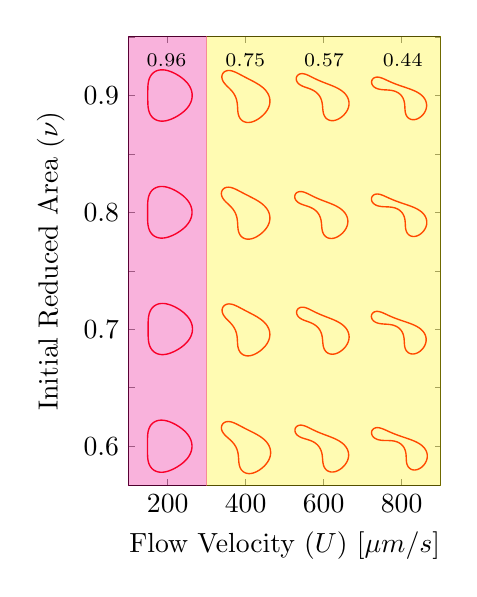
\begin{tikzpicture}[scale=1.0]

\pgfmathsetlengthmacro\MajorTickLength{
      \pgfkeysvalueof{/pgfplots/major tick length} * 0.5
    }

  \begin{axis}[
    major tick length=\MajorTickLength,
    compat=newest,
    axis equal image,
    xmin = -2,
    xmax = 30,
    ymin = -2,
    ymax = 44,
    xtick = {2,10,18,26},
    xticklabels = {$200$,$400$,$600$,$800$},
    xlabel = {Flow Velocity ($U$) [$\mu m/s$]},
    ytick = {2,8,14,20,26,32,38,44},
    yticklabels = {$0.6$,,$0.7$,,$0.8$,,$0.9$,},
    ylabel = {Initial Reduced Area ($\nu$)},
    ylabel near ticks,
%    ylabel shift = {-0.3cm},
  ]

% RA = 0.60,flow rate = 200
\addplot[red,line width=0.5pt] coordinates{
(4.4637e+00,2.3139e+00)
(4.4540e+00,2.3639e+00)
(4.4426e+00,2.4150e+00)
(4.4291e+00,2.4682e+00)
(4.4129e+00,2.5245e+00)
(4.3934e+00,2.5846e+00)
(4.3702e+00,2.6489e+00)
(4.3426e+00,2.7174e+00)
(4.3099e+00,2.7903e+00)
(4.2715e+00,2.8674e+00)
(4.2270e+00,2.9482e+00)
(4.1758e+00,3.0324e+00)
(4.1175e+00,3.1195e+00)
(4.0517e+00,3.2090e+00)
(3.9784e+00,3.3002e+00)
(3.8973e+00,3.3926e+00)
(3.8085e+00,3.4857e+00)
(3.7120e+00,3.5790e+00)
(3.6081e+00,3.6719e+00)
(3.4970e+00,3.7641e+00)
(3.3790e+00,3.8552e+00)
(3.2544e+00,3.9449e+00)
(3.1236e+00,4.0329e+00)
(2.9870e+00,4.1187e+00)
(2.8448e+00,4.2020e+00)
(2.6974e+00,4.2822e+00)
(2.5449e+00,4.3586e+00)
(2.3876e+00,4.4303e+00)
(2.2257e+00,4.4962e+00)
(2.0594e+00,4.5548e+00)
(1.8889e+00,4.6045e+00)
(1.7148e+00,4.6430e+00)
(1.5378e+00,4.6681e+00)
(1.3594e+00,4.6772e+00)
(1.1814e+00,4.6680e+00)
(1.0063e+00,4.6386e+00)
(8.3760e-01,4.5877e+00)
(6.7865e-01,4.5153e+00)
(5.3294e-01,4.4225e+00)
(4.0333e-01,4.3119e+00)
(2.9164e-01,4.1868e+00)
(1.9847e-01,4.0511e+00)
(1.2326e-01,3.9084e+00)
(6.4522e-02,3.7623e+00)
(2.0152e-02,3.6154e+00)
(-1.2200e-02,3.4699e+00)
(-3.4892e-02,3.3273e+00)
(-5.0101e-02,3.1887e+00)
(-5.9730e-02,3.0549e+00)
(-6.5363e-02,2.9263e+00)
(-6.8267e-02,2.8034e+00)
(-6.9417e-02,2.6863e+00)
(-6.9531e-02,2.5753e+00)
(-6.9115e-02,2.4705e+00)
(-6.8504e-02,2.3719e+00)
(-6.7904e-02,2.2796e+00)
(-6.7423e-02,2.1935e+00)
(-6.7106e-02,2.1136e+00)
(-6.6955e-02,2.0397e+00)
(-6.6950e-02,1.9713e+00)
(-6.7061e-02,1.9082e+00)
(-6.7257e-02,1.8496e+00)
(-6.7512e-02,1.7946e+00)
(-6.7806e-02,1.7423e+00)
(-6.8126e-02,1.6914e+00)
(-6.8462e-02,1.6404e+00)
(-6.8802e-02,1.5881e+00)
(-6.9127e-02,1.5332e+00)
(-6.9401e-02,1.4746e+00)
(-6.9561e-02,1.4114e+00)
(-6.9506e-02,1.3431e+00)
(-6.9079e-02,1.2691e+00)
(-6.8049e-02,1.1892e+00)
(-6.6087e-02,1.1032e+00)
(-6.2740e-02,1.0109e+00)
(-5.7399e-02,9.1249e-01)
(-4.9269e-02,8.0795e-01)
(-3.7337e-02,6.9757e-01)
(-2.0353e-02,5.8173e-01)
(3.1833e-03,4.6103e-01)
(3.5002e-02,3.3635e-01)
(7.7010e-02,2.0894e-01)
(1.3118e-01,8.0509e-02)
(1.9939e-01,-4.6728e-02)
(2.8317e-01,-1.7001e-01)
(3.8346e-01,-2.8614e-01)
(5.0038e-01,-3.9171e-01)
(6.3304e-01,-4.8342e-01)
(7.7965e-01,-5.5846e-01)
(9.3765e-01,-6.1490e-01)
(1.1041e+00,-6.5185e-01)
(1.2760e+00,-6.6945e-01)
(1.4508e+00,-6.6878e-01)
(1.6264e+00,-6.5150e-01)
(1.8011e+00,-6.1963e-01)
(1.9739e+00,-5.7523e-01)
(2.1441e+00,-5.2029e-01)
(2.3112e+00,-4.5656e-01)
(2.4749e+00,-3.8553e-01)
(2.6349e+00,-3.0838e-01)
(2.7910e+00,-2.2607e-01)
(2.9429e+00,-1.3931e-01)
(3.0901e+00,-4.8601e-02)
(3.2323e+00,4.5669e-02)
(3.3690e+00,1.4322e-01)
(3.4995e+00,2.4384e-01)
(3.6234e+00,3.4728e-01)
(3.7401e+00,4.5331e-01)
(3.8489e+00,5.6161e-01)
(3.9495e+00,6.7177e-01)
(4.0412e+00,7.8329e-01)
(4.1239e+00,8.9556e-01)
(4.1973e+00,1.0079e+00)
(4.2614e+00,1.1194e+00)
(4.3164e+00,1.2294e+00)
(4.3625e+00,1.3371e+00)
(4.4002e+00,1.4415e+00)
(4.4302e+00,1.5419e+00)
(4.4532e+00,1.6378e+00)
(4.4699e+00,1.7286e+00)
(4.4813e+00,1.8138e+00)
(4.4881e+00,1.8935e+00)
(4.4912e+00,1.9673e+00)
(4.4912e+00,2.0356e+00)
(4.4889e+00,2.0987e+00)
(4.4847e+00,2.1572e+00)
(4.4790e+00,2.2118e+00)
(4.4720e+00,2.2637e+00)
(4.4637e+00,2.3139e+00)
};

% RA = 0.70,flow rate = 200
\addplot[red,line width=0.5pt] coordinates{
(9.0104e-01,1.1507e+01)
(9.5947e-01,1.1485e+01)
(1.0198e+00,1.1465e+01)
(1.0827e+00,1.1448e+01)
(1.1490e+00,1.1433e+01)
(1.2192e+00,1.1421e+01)
(1.2939e+00,1.1411e+01)
(1.3732e+00,1.1405e+01)
(1.4575e+00,1.1403e+01)
(1.5468e+00,1.1404e+01)
(1.6410e+00,1.1411e+01)
(1.7400e+00,1.1423e+01)
(1.8435e+00,1.1440e+01)
(1.9513e+00,1.1463e+01)
(2.0630e+00,1.1492e+01)
(2.1783e+00,1.1526e+01)
(2.2969e+00,1.1567e+01)
(2.4184e+00,1.1614e+01)
(2.5424e+00,1.1667e+01)
(2.6687e+00,1.1725e+01)
(2.7968e+00,1.1789e+01)
(2.9263e+00,1.1859e+01)
(3.0567e+00,1.1935e+01)
(3.1877e+00,1.2016e+01)
(3.3184e+00,1.2103e+01)
(3.4484e+00,1.2196e+01)
(3.5767e+00,1.2295e+01)
(3.7024e+00,1.2401e+01)
(3.8244e+00,1.2514e+01)
(3.9416e+00,1.2634e+01)
(4.0525e+00,1.2760e+01)
(4.1557e+00,1.2894e+01)
(4.2497e+00,1.3035e+01)
(4.3330e+00,1.3183e+01)
(4.4039e+00,1.3337e+01)
(4.4612e+00,1.3495e+01)
(4.5039e+00,1.3657e+01)
(4.5312e+00,1.3821e+01)
(4.5429e+00,1.3985e+01)
(4.5393e+00,1.4147e+01)
(4.5211e+00,1.4305e+01)
(4.4893e+00,1.4459e+01)
(4.4455e+00,1.4607e+01)
(4.3912e+00,1.4747e+01)
(4.3281e+00,1.4880e+01)
(4.2579e+00,1.5005e+01)
(4.1824e+00,1.5122e+01)
(4.1028e+00,1.5231e+01)
(4.0208e+00,1.5332e+01)
(3.9373e+00,1.5425e+01)
(3.8535e+00,1.5512e+01)
(3.7703e+00,1.5591e+01)
(3.6884e+00,1.5665e+01)
(3.6083e+00,1.5733e+01)
(3.5306e+00,1.5795e+01)
(3.4556e+00,1.5853e+01)
(3.3835e+00,1.5905e+01)
(3.3145e+00,1.5954e+01)
(3.2486e+00,1.5998e+01)
(3.1856e+00,1.6039e+01)
(3.1253e+00,1.6078e+01)
(3.0673e+00,1.6113e+01)
(3.0112e+00,1.6146e+01)
(2.9562e+00,1.6178e+01)
(2.9017e+00,1.6209e+01)
(2.8468e+00,1.6238e+01)
(2.7907e+00,1.6268e+01)
(2.7325e+00,1.6298e+01)
(2.6716e+00,1.6328e+01)
(2.6071e+00,1.6358e+01)
(2.5386e+00,1.6389e+01)
(2.4655e+00,1.6421e+01)
(2.3875e+00,1.6453e+01)
(2.3040e+00,1.6484e+01)
(2.2150e+00,1.6516e+01)
(2.1200e+00,1.6546e+01)
(2.0191e+00,1.6574e+01)
(1.9120e+00,1.6600e+01)
(1.7988e+00,1.6622e+01)
(1.6796e+00,1.6639e+01)
(1.5547e+00,1.6649e+01)
(1.4246e+00,1.6651e+01)
(1.2902e+00,1.6642e+01)
(1.1528e+00,1.6622e+01)
(1.0139e+00,1.6587e+01)
(8.7594e-01,1.6536e+01)
(7.4137e-01,1.6468e+01)
(6.1309e-01,1.6383e+01)
(4.9394e-01,1.6281e+01)
(3.8644e-01,1.6163e+01)
(2.9249e-01,1.6031e+01)
(2.1314e-01,1.5887e+01)
(1.4850e-01,1.5734e+01)
(9.7889e-02,1.5575e+01)
(5.9914e-02,1.5411e+01)
(3.2772e-02,1.5244e+01)
(1.4445e-02,1.5075e+01)
(2.9083e-03,1.4906e+01)
(-3.7244e-03,1.4737e+01)
(-7.0909e-03,1.4568e+01)
(-8.5139e-03,1.4401e+01)
(-8.9644e-03,1.4235e+01)
(-9.0511e-03,1.4070e+01)
(-9.0320e-03,1.3908e+01)
(-8.8434e-03,1.3748e+01)
(-8.1438e-03,1.3591e+01)
(-6.3705e-03,1.3437e+01)
(-2.8029e-03,1.3286e+01)
(3.3682e-03,1.3139e+01)
(1.2970e-02,1.2996e+01)
(2.6777e-02,1.2858e+01)
(4.5448e-02,1.2725e+01)
(6.9469e-02,1.2597e+01)
(9.9105e-02,1.2475e+01)
(1.3438e-01,1.2360e+01)
(1.7506e-01,1.2252e+01)
(2.2069e-01,1.2151e+01)
(2.7061e-01,1.2059e+01)
(3.2402e-01,1.1975e+01)
(3.8004e-01,1.1899e+01)
(4.3782e-01,1.1831e+01)
(4.9653e-01,1.1770e+01)
(5.5550e-01,1.1717e+01)
(6.1421e-01,1.1670e+01)
(6.7235e-01,1.1629e+01)
(7.2985e-01,1.1592e+01)
(7.8686e-01,1.1561e+01)
(8.4373e-01,1.1532e+01)
(9.0104e-01,1.1507e+01)
};

% RA = 0.80,flow rate = 200
\addplot[red,line width=0.5pt] coordinates{
(-5.9686e-02,2.5616e+01)
(-5.9666e-02,2.5542e+01)
(-5.9452e-02,2.5468e+01)
(-5.8940e-02,2.5392e+01)
(-5.7992e-02,2.5314e+01)
(-5.6422e-02,2.5233e+01)
(-5.3984e-02,2.5150e+01)
(-5.0358e-02,2.5063e+01)
(-4.5129e-02,2.4973e+01)
(-3.7771e-02,2.4878e+01)
(-2.7629e-02,2.4780e+01)
(-1.3901e-02,2.4678e+01)
(4.3702e-03,2.4572e+01)
(2.8302e-02,2.4462e+01)
(5.9156e-02,2.4350e+01)
(9.8306e-02,2.4236e+01)
(1.4717e-01,2.4121e+01)
(2.0713e-01,2.4007e+01)
(2.7937e-01,2.3895e+01)
(3.6475e-01,2.3788e+01)
(4.6366e-01,2.3688e+01)
(5.7586e-01,2.3598e+01)
(7.0050e-01,2.3520e+01)
(8.3610e-01,2.3456e+01)
(9.8076e-01,2.3407e+01)
(1.1323e+00,2.3374e+01)
(1.2886e+00,2.3357e+01)
(1.4477e+00,2.3355e+01)
(1.6079e+00,2.3367e+01)
(1.7680e+00,2.3392e+01)
(1.9269e+00,2.3427e+01)
(2.0840e+00,2.3473e+01)
(2.2388e+00,2.3526e+01)
(2.3911e+00,2.3587e+01)
(2.5405e+00,2.3653e+01)
(2.6869e+00,2.3725e+01)
(2.8299e+00,2.3800e+01)
(2.9694e+00,2.3880e+01)
(3.1050e+00,2.3964e+01)
(3.2364e+00,2.4050e+01)
(3.3631e+00,2.4140e+01)
(3.4848e+00,2.4232e+01)
(3.6010e+00,2.4327e+01)
(3.7112e+00,2.4424e+01)
(3.8150e+00,2.4524e+01)
(3.9120e+00,2.4626e+01)
(4.0017e+00,2.4729e+01)
(4.0838e+00,2.4834e+01)
(4.1581e+00,2.4940e+01)
(4.2245e+00,2.5046e+01)
(4.2829e+00,2.5151e+01)
(4.3335e+00,2.5256e+01)
(4.3763e+00,2.5359e+01)
(4.4119e+00,2.5461e+01)
(4.4404e+00,2.5560e+01)
(4.4625e+00,2.5656e+01)
(4.4787e+00,2.5749e+01)
(4.4896e+00,2.5839e+01)
(4.4956e+00,2.5926e+01)
(4.4973e+00,2.6010e+01)
(4.4952e+00,2.6090e+01)
(4.4896e+00,2.6168e+01)
(4.4809e+00,2.6243e+01)
(4.4691e+00,2.6317e+01)
(4.4545e+00,2.6389e+01)
(4.4370e+00,2.6461e+01)
(4.4163e+00,2.6532e+01)
(4.3924e+00,2.6604e+01)
(4.3649e+00,2.6677e+01)
(4.3336e+00,2.6751e+01)
(4.2979e+00,2.6827e+01)
(4.2577e+00,2.6904e+01)
(4.2124e+00,2.6982e+01)
(4.1619e+00,2.7062e+01)
(4.1057e+00,2.7143e+01)
(4.0437e+00,2.7226e+01)
(3.9757e+00,2.7309e+01)
(3.9015e+00,2.7393e+01)
(3.8211e+00,2.7477e+01)
(3.7346e+00,2.7561e+01)
(3.6420e+00,2.7645e+01)
(3.5434e+00,2.7728e+01)
(3.4390e+00,2.7811e+01)
(3.3290e+00,2.7892e+01)
(3.2137e+00,2.7973e+01)
(3.0932e+00,2.8051e+01)
(2.9677e+00,2.8128e+01)
(2.8375e+00,2.8203e+01)
(2.7028e+00,2.8275e+01)
(2.5638e+00,2.8343e+01)
(2.4205e+00,2.8408e+01)
(2.2731e+00,2.8468e+01)
(2.1219e+00,2.8522e+01)
(1.9670e+00,2.8569e+01)
(1.8087e+00,2.8608e+01)
(1.6477e+00,2.8635e+01)
(1.4847e+00,2.8651e+01)
(1.3209e+00,2.8652e+01)
(1.1582e+00,2.8637e+01)
(9.9868e-01,2.8605e+01)
(8.4486e-01,2.8555e+01)
(6.9951e-01,2.8487e+01)
(5.6524e-01,2.8402e+01)
(4.4425e-01,2.8301e+01)
(3.3804e-01,2.8188e+01)
(2.4725e-01,2.8066e+01)
(1.7170e-01,2.7936e+01)
(1.1047e-01,2.7802e+01)
(6.2142e-02,2.7667e+01)
(2.5006e-02,2.7531e+01)
(-2.7489e-03,2.7397e+01)
(-2.2883e-02,2.7266e+01)
(-3.7010e-02,2.7137e+01)
(-4.6543e-02,2.7013e+01)
(-5.2674e-02,2.6892e+01)
(-5.6374e-02,2.6776e+01)
(-5.8410e-02,2.6664e+01)
(-5.9368e-02,2.6556e+01)
(-5.9680e-02,2.6453e+01)
(-5.9649e-02,2.6354e+01)
(-5.9481e-02,2.6260e+01)
(-5.9301e-02,2.6169e+01)
(-5.9177e-02,2.6082e+01)
(-5.9138e-02,2.5999e+01)
(-5.9184e-02,2.5918e+01)
(-5.9297e-02,2.5840e+01)
(-5.9446e-02,2.5765e+01)
(-5.9592e-02,2.5690e+01)
(-5.9686e-02,2.5616e+01)
};

% RA = 0.90,flow rate = 200
\addplot[red,line width=0.5pt] coordinates{
(-8.5612e-03,3.9169e+01)
(-1.7779e-02,3.9080e+01)
(-2.5016e-02,3.8990e+01)
(-3.0572e-02,3.8899e+01)
(-3.4712e-02,3.8807e+01)
(-3.7677e-02,3.8714e+01)
(-3.9686e-02,3.8618e+01)
(-4.0944e-02,3.8521e+01)
(-4.1641e-02,3.8421e+01)
(-4.1955e-02,3.8318e+01)
(-4.2042e-02,3.8213e+01)
(-4.2032e-02,3.8105e+01)
(-4.2016e-02,3.7994e+01)
(-4.2031e-02,3.7880e+01)
(-4.2042e-02,3.7763e+01)
(-4.1923e-02,3.7643e+01)
(-4.1435e-02,3.7520e+01)
(-4.0202e-02,3.7394e+01)
(-3.7691e-02,3.7265e+01)
(-3.3194e-02,3.7134e+01)
(-2.5810e-02,3.7000e+01)
(-1.4443e-02,3.6864e+01)
(2.1944e-03,3.6726e+01)
(2.5552e-02,3.6587e+01)
(5.7194e-02,3.6447e+01)
(9.8715e-02,3.6308e+01)
(1.5162e-01,3.6172e+01)
(2.1719e-01,3.6039e+01)
(2.9626e-01,3.5913e+01)
(3.8913e-01,3.5795e+01)
(4.9541e-01,3.5688e+01)
(6.1401e-01,3.5595e+01)
(7.4320e-01,3.5516e+01)
(8.8083e-01,3.5453e+01)
(1.0245e+00,3.5406e+01)
(1.1720e+00,3.5375e+01)
(1.3211e+00,3.5359e+01)
(1.4701e+00,3.5357e+01)
(1.6177e+00,3.5366e+01)
(1.7629e+00,3.5386e+01)
(1.9049e+00,3.5415e+01)
(2.0434e+00,3.5451e+01)
(2.1781e+00,3.5494e+01)
(2.3089e+00,3.5541e+01)
(2.4356e+00,3.5592e+01)
(2.5583e+00,3.5647e+01)
(2.6769e+00,3.5703e+01)
(2.7915e+00,3.5762e+01)
(2.9020e+00,3.5823e+01)
(3.0084e+00,3.5884e+01)
(3.1108e+00,3.5947e+01)
(3.2091e+00,3.6011e+01)
(3.3033e+00,3.6075e+01)
(3.3935e+00,3.6139e+01)
(3.4797e+00,3.6205e+01)
(3.5621e+00,3.6270e+01)
(3.6405e+00,3.6336e+01)
(3.7153e+00,3.6402e+01)
(3.7865e+00,3.6469e+01)
(3.8542e+00,3.6536e+01)
(3.9186e+00,3.6604e+01)
(3.9799e+00,3.6673e+01)
(4.0381e+00,3.6743e+01)
(4.0935e+00,3.6814e+01)
(4.1461e+00,3.6887e+01)
(4.1959e+00,3.6961e+01)
(4.2430e+00,3.7038e+01)
(4.2874e+00,3.7118e+01)
(4.3288e+00,3.7200e+01)
(4.3670e+00,3.7285e+01)
(4.4019e+00,3.7374e+01)
(4.4328e+00,3.7467e+01)
(4.4595e+00,3.7563e+01)
(4.4814e+00,3.7663e+01)
(4.4979e+00,3.7767e+01)
(4.5083e+00,3.7874e+01)
(4.5121e+00,3.7985e+01)
(4.5086e+00,3.8099e+01)
(4.4973e+00,3.8216e+01)
(4.4778e+00,3.8334e+01)
(4.4496e+00,3.8454e+01)
(4.4126e+00,3.8574e+01)
(4.3666e+00,3.8694e+01)
(4.3116e+00,3.8814e+01)
(4.2480e+00,3.8932e+01)
(4.1759e+00,3.9048e+01)
(4.0958e+00,3.9161e+01)
(4.0083e+00,3.9272e+01)
(3.9138e+00,3.9380e+01)
(3.8130e+00,3.9484e+01)
(3.7065e+00,3.9584e+01)
(3.5949e+00,3.9681e+01)
(3.4787e+00,3.9775e+01)
(3.3585e+00,3.9865e+01)
(3.2348e+00,3.9951e+01)
(3.1081e+00,4.0033e+01)
(2.9787e+00,4.0112e+01)
(2.8470e+00,4.0186e+01)
(2.7133e+00,4.0257e+01)
(2.5778e+00,4.0323e+01)
(2.4409e+00,4.0384e+01)
(2.3027e+00,4.0440e+01)
(2.1635e+00,4.0490e+01)
(2.0234e+00,4.0533e+01)
(1.8830e+00,4.0568e+01)
(1.7425e+00,4.0596e+01)
(1.6025e+00,4.0614e+01)
(1.4639e+00,4.0622e+01)
(1.3273e+00,4.0620e+01)
(1.1938e+00,4.0607e+01)
(1.0646e+00,4.0583e+01)
(9.4077e-01,4.0548e+01)
(8.2346e-01,4.0502e+01)
(7.1366e-01,4.0447e+01)
(6.1219e-01,4.0383e+01)
(5.1958e-01,4.0311e+01)
(4.3610e-01,4.0234e+01)
(3.6173e-01,4.0152e+01)
(2.9622e-01,4.0066e+01)
(2.3908e-01,3.9978e+01)
(1.8972e-01,3.9888e+01)
(1.4744e-01,3.9797e+01)
(1.1151e-01,3.9707e+01)
(8.1192e-02,3.9616e+01)
(5.5796e-02,3.9526e+01)
(3.4673e-02,3.9437e+01)
(1.7241e-02,3.9347e+01)
(2.9806e-03,3.9258e+01)
(-8.5612e-03,3.9169e+01)
};

% RA = 0.60,flow rate = 400
\addplot[red,line width=0.5pt] coordinates{
(7.6317e+00,4.2622e+00)
(7.6034e+00,4.2195e+00)
(7.5781e+00,4.1732e+00)
(7.5560e+00,4.1225e+00)
(7.5375e+00,4.0665e+00)
(7.5235e+00,4.0045e+00)
(7.5151e+00,3.9362e+00)
(7.5139e+00,3.8618e+00)
(7.5212e+00,3.7817e+00)
(7.5383e+00,3.6968e+00)
(7.5662e+00,3.6082e+00)
(7.6056e+00,3.5170e+00)
(7.6566e+00,3.4246e+00)
(7.7189e+00,3.3319e+00)
(7.7921e+00,3.2394e+00)
(7.8750e+00,3.1474e+00)
(7.9666e+00,3.0558e+00)
(8.0656e+00,2.9637e+00)
(8.1704e+00,2.8703e+00)
(8.2796e+00,2.7743e+00)
(8.3915e+00,2.6740e+00)
(8.5041e+00,2.5680e+00)
(8.6154e+00,2.4549e+00)
(8.7233e+00,2.3334e+00)
(8.8256e+00,2.2027e+00)
(8.9200e+00,2.0625e+00)
(9.0046e+00,1.9131e+00)
(9.0776e+00,1.7550e+00)
(9.1382e+00,1.5897e+00)
(9.1860e+00,1.4186e+00)
(9.2217e+00,1.2434e+00)
(9.2468e+00,1.0655e+00)
(9.2639e+00,8.8621e-01)
(9.2762e+00,7.0655e-01)
(9.2878e+00,5.2725e-01)
(9.3032e+00,3.4904e-01)
(9.3273e+00,1.7302e-01)
(9.3648e+00,1.0196e-03)
(9.4198e+00,-1.6408e-01)
(9.4952e+00,-3.1828e-01)
(9.5917e+00,-4.5686e-01)
(9.7078e+00,-5.7517e-01)
(9.8398e+00,-6.6968e-01)
(9.9825e+00,-7.3875e-01)
(1.0131e+01,-7.8285e-01)
(1.0279e+01,-8.0417e-01)
(1.0424e+01,-8.0600e-01)
(1.0564e+01,-7.9200e-01)
(1.0697e+01,-7.6569e-01)
(1.0821e+01,-7.3023e-01)
(1.0938e+01,-6.8825e-01)
(1.1046e+01,-6.4192e-01)
(1.1147e+01,-5.9295e-01)
(1.1239e+01,-5.4270e-01)
(1.1325e+01,-4.9225e-01)
(1.1403e+01,-4.4244e-01)
(1.1475e+01,-3.9388e-01)
(1.1541e+01,-3.4707e-01)
(1.1600e+01,-3.0231e-01)
(1.1654e+01,-2.5977e-01)
(1.1703e+01,-2.1946e-01)
(1.1748e+01,-1.8119e-01)
(1.1790e+01,-1.4458e-01)
(1.1829e+01,-1.0907e-01)
(1.1866e+01,-7.3859e-02)
(1.1903e+01,-3.8038e-02)
(1.1940e+01,-6.1479e-04)
(1.1978e+01,3.9385e-02)
(1.2018e+01,8.2865e-02)
(1.2060e+01,1.3063e-01)
(1.2104e+01,1.8341e-01)
(1.2150e+01,2.4182e-01)
(1.2198e+01,3.0645e-01)
(1.2247e+01,3.7781e-01)
(1.2297e+01,4.5639e-01)
(1.2346e+01,5.4259e-01)
(1.2394e+01,6.3678e-01)
(1.2439e+01,7.3919e-01)
(1.2479e+01,8.4994e-01)
(1.2514e+01,9.6892e-01)
(1.2540e+01,1.0958e+00)
(1.2556e+01,1.2299e+00)
(1.2561e+01,1.3702e+00)
(1.2552e+01,1.5153e+00)
(1.2529e+01,1.6636e+00)
(1.2490e+01,1.8131e+00)
(1.2435e+01,1.9620e+00)
(1.2364e+01,2.1084e+00)
(1.2279e+01,2.2505e+00)
(1.2180e+01,2.3872e+00)
(1.2068e+01,2.5176e+00)
(1.1945e+01,2.6411e+00)
(1.1813e+01,2.7577e+00)
(1.1673e+01,2.8675e+00)
(1.1528e+01,2.9711e+00)
(1.1377e+01,3.0689e+00)
(1.1223e+01,3.1618e+00)
(1.1066e+01,3.2505e+00)
(1.0908e+01,3.3357e+00)
(1.0749e+01,3.4181e+00)
(1.0591e+01,3.4984e+00)
(1.0433e+01,3.5772e+00)
(1.0277e+01,3.6549e+00)
(1.0124e+01,3.7318e+00)
(9.9728e+00,3.8081e+00)
(9.8251e+00,3.8837e+00)
(9.6809e+00,3.9586e+00)
(9.5403e+00,4.0323e+00)
(9.4035e+00,4.1043e+00)
(9.2704e+00,4.1739e+00)
(9.1410e+00,4.2402e+00)
(9.0150e+00,4.3023e+00)
(8.8924e+00,4.3590e+00)
(8.7730e+00,4.4093e+00)
(8.6568e+00,4.4522e+00)
(8.5441e+00,4.4866e+00)
(8.4352e+00,4.5119e+00)
(8.3308e+00,4.5276e+00)
(8.2318e+00,4.5337e+00)
(8.1389e+00,4.5306e+00)
(8.0531e+00,4.5190e+00)
(7.9749e+00,4.5001e+00)
(7.9048e+00,4.4752e+00)
(7.8426e+00,4.4456e+00)
(7.7882e+00,4.4128e+00)
(7.7408e+00,4.3777e+00)
(7.6995e+00,4.3409e+00)
(7.6635e+00,4.3025e+00)
(7.6317e+00,4.2622e+00)
};

% RA = 0.70,flow rate = 400
\addplot[red,line width=0.5pt] coordinates{
(9.2832e+00,1.1931e+01)
(9.3071e+00,1.1873e+01)
(9.3344e+00,1.1815e+01)
(9.3658e+00,1.1757e+01)
(9.4021e+00,1.1699e+01)
(9.4442e+00,1.1641e+01)
(9.4930e+00,1.1583e+01)
(9.5495e+00,1.1526e+01)
(9.6143e+00,1.1471e+01)
(9.6882e+00,1.1420e+01)
(9.7712e+00,1.1373e+01)
(9.8635e+00,1.1334e+01)
(9.9644e+00,1.1303e+01)
(1.0073e+01,1.1281e+01)
(1.0189e+01,1.1271e+01)
(1.0310e+01,1.1273e+01)
(1.0436e+01,1.1286e+01)
(1.0564e+01,1.1312e+01)
(1.0695e+01,1.1349e+01)
(1.0827e+01,1.1397e+01)
(1.0959e+01,1.1456e+01)
(1.1090e+01,1.1523e+01)
(1.1222e+01,1.1600e+01)
(1.1352e+01,1.1685e+01)
(1.1480e+01,1.1777e+01)
(1.1606e+01,1.1877e+01)
(1.1729e+01,1.1985e+01)
(1.1848e+01,1.2100e+01)
(1.1962e+01,1.2222e+01)
(1.2069e+01,1.2353e+01)
(1.2168e+01,1.2491e+01)
(1.2257e+01,1.2636e+01)
(1.2333e+01,1.2789e+01)
(1.2395e+01,1.2948e+01)
(1.2442e+01,1.3112e+01)
(1.2471e+01,1.3279e+01)
(1.2482e+01,1.3447e+01)
(1.2475e+01,1.3614e+01)
(1.2450e+01,1.3778e+01)
(1.2409e+01,1.3936e+01)
(1.2352e+01,1.4087e+01)
(1.2283e+01,1.4229e+01)
(1.2203e+01,1.4362e+01)
(1.2115e+01,1.4486e+01)
(1.2021e+01,1.4600e+01)
(1.1922e+01,1.4705e+01)
(1.1821e+01,1.4802e+01)
(1.1718e+01,1.4891e+01)
(1.1616e+01,1.4973e+01)
(1.1514e+01,1.5048e+01)
(1.1415e+01,1.5117e+01)
(1.1318e+01,1.5181e+01)
(1.1224e+01,1.5240e+01)
(1.1133e+01,1.5295e+01)
(1.1047e+01,1.5345e+01)
(1.0964e+01,1.5392e+01)
(1.0885e+01,1.5436e+01)
(1.0811e+01,1.5477e+01)
(1.0740e+01,1.5515e+01)
(1.0673e+01,1.5551e+01)
(1.0610e+01,1.5584e+01)
(1.0549e+01,1.5616e+01)
(1.0491e+01,1.5646e+01)
(1.0434e+01,1.5676e+01)
(1.0378e+01,1.5705e+01)
(1.0322e+01,1.5734e+01)
(1.0265e+01,1.5763e+01)
(1.0207e+01,1.5793e+01)
(1.0146e+01,1.5825e+01)
(1.0083e+01,1.5858e+01)
(1.0015e+01,1.5893e+01)
(9.9444e+00,1.5930e+01)
(9.8692e+00,1.5970e+01)
(9.7896e+00,1.6012e+01)
(9.7056e+00,1.6057e+01)
(9.6169e+00,1.6104e+01)
(9.5236e+00,1.6153e+01)
(9.4255e+00,1.6205e+01)
(9.3225e+00,1.6259e+01)
(9.2145e+00,1.6314e+01)
(9.1011e+00,1.6370e+01)
(8.9821e+00,1.6425e+01)
(8.8570e+00,1.6477e+01)
(8.7253e+00,1.6525e+01)
(8.5866e+00,1.6565e+01)
(8.4410e+00,1.6592e+01)
(8.2896e+00,1.6602e+01)
(8.1353e+00,1.6587e+01)
(7.9836e+00,1.6543e+01)
(7.8432e+00,1.6465e+01)
(7.7247e+00,1.6353e+01)
(7.6383e+00,1.6212e+01)
(7.5908e+00,1.6052e+01)
(7.5836e+00,1.5884e+01)
(7.6133e+00,1.5717e+01)
(7.6736e+00,1.5558e+01)
(7.7571e+00,1.5409e+01)
(7.8569e+00,1.5271e+01)
(7.9674e+00,1.5141e+01)
(8.0839e+00,1.5017e+01)
(8.2026e+00,1.4898e+01)
(8.3204e+00,1.4779e+01)
(8.4349e+00,1.4659e+01)
(8.5438e+00,1.4537e+01)
(8.6454e+00,1.4412e+01)
(8.7381e+00,1.4284e+01)
(8.8210e+00,1.4153e+01)
(8.8932e+00,1.4019e+01)
(8.9547e+00,1.3885e+01)
(9.0057e+00,1.3750e+01)
(9.0467e+00,1.3616e+01)
(9.0788e+00,1.3484e+01)
(9.1031e+00,1.3355e+01)
(9.1210e+00,1.3230e+01)
(9.1339e+00,1.3109e+01)
(9.1431e+00,1.2993e+01)
(9.1498e+00,1.2883e+01)
(9.1552e+00,1.2777e+01)
(9.1602e+00,1.2677e+01)
(9.1656e+00,1.2582e+01)
(9.1720e+00,1.2492e+01)
(9.1796e+00,1.2407e+01)
(9.1888e+00,1.2328e+01)
(9.1997e+00,1.2253e+01)
(9.2124e+00,1.2182e+01)
(9.2270e+00,1.2115e+01)
(9.2435e+00,1.2051e+01)
(9.2622e+00,1.1990e+01)
(9.2832e+00,1.1931e+01)
};

% RA = 0.80,flow rate = 400
\addplot[red,line width=0.5pt] coordinates{
(1.0564e+01,2.7552e+01)
(1.0498e+01,2.7585e+01)
(1.0431e+01,2.7620e+01)
(1.0363e+01,2.7654e+01)
(1.0293e+01,2.7690e+01)
(1.0221e+01,2.7726e+01)
(1.0146e+01,2.7765e+01)
(1.0068e+01,2.7804e+01)
(9.9864e+00,2.7846e+01)
(9.9016e+00,2.7890e+01)
(9.8133e+00,2.7936e+01)
(9.7212e+00,2.7984e+01)
(9.6253e+00,2.8034e+01)
(9.5255e+00,2.8087e+01)
(9.4218e+00,2.8142e+01)
(9.3142e+00,2.8198e+01)
(9.2024e+00,2.8256e+01)
(9.0863e+00,2.8315e+01)
(8.9654e+00,2.8373e+01)
(8.8395e+00,2.8429e+01)
(8.7078e+00,2.8481e+01)
(8.5700e+00,2.8526e+01)
(8.4258e+00,2.8560e+01)
(8.2759e+00,2.8579e+01)
(8.1222e+00,2.8576e+01)
(7.9691e+00,2.8545e+01)
(7.8238e+00,2.8483e+01)
(7.6960e+00,2.8387e+01)
(7.5959e+00,2.8260e+01)
(7.5318e+00,2.8111e+01)
(7.5070e+00,2.7949e+01)
(7.5202e+00,2.7785e+01)
(7.5661e+00,2.7627e+01)
(7.6377e+00,2.7478e+01)
(7.7284e+00,2.7341e+01)
(7.8319e+00,2.7213e+01)
(7.9435e+00,2.7095e+01)
(8.0593e+00,2.6981e+01)
(8.1762e+00,2.6872e+01)
(8.2917e+00,2.6763e+01)
(8.4038e+00,2.6654e+01)
(8.5106e+00,2.6543e+01)
(8.6108e+00,2.6430e+01)
(8.7031e+00,2.6314e+01)
(8.7867e+00,2.6196e+01)
(8.8610e+00,2.6075e+01)
(8.9258e+00,2.5953e+01)
(8.9812e+00,2.5831e+01)
(9.0275e+00,2.5710e+01)
(9.0655e+00,2.5590e+01)
(9.0959e+00,2.5472e+01)
(9.1198e+00,2.5357e+01)
(9.1382e+00,2.5246e+01)
(9.1521e+00,2.5138e+01)
(9.1626e+00,2.5035e+01)
(9.1706e+00,2.4936e+01)
(9.1769e+00,2.4840e+01)
(9.1822e+00,2.4749e+01)
(9.1872e+00,2.4662e+01)
(9.1924e+00,2.4578e+01)
(9.1983e+00,2.4497e+01)
(9.2051e+00,2.4419e+01)
(9.2133e+00,2.4343e+01)
(9.2233e+00,2.4269e+01)
(9.2354e+00,2.4195e+01)
(9.2501e+00,2.4122e+01)
(9.2680e+00,2.4049e+01)
(9.2896e+00,2.3976e+01)
(9.3159e+00,2.3902e+01)
(9.3475e+00,2.3827e+01)
(9.3856e+00,2.3752e+01)
(9.4311e+00,2.3678e+01)
(9.4850e+00,2.3604e+01)
(9.5482e+00,2.3533e+01)
(9.6214e+00,2.3465e+01)
(9.7050e+00,2.3404e+01)
(9.7989e+00,2.3350e+01)
(9.9025e+00,2.3305e+01)
(1.0015e+01,2.3272e+01)
(1.0135e+01,2.3251e+01)
(1.0260e+01,2.3244e+01)
(1.0390e+01,2.3250e+01)
(1.0523e+01,2.3269e+01)
(1.0657e+01,2.3301e+01)
(1.0792e+01,2.3345e+01)
(1.0926e+01,2.3399e+01)
(1.1060e+01,2.3463e+01)
(1.1192e+01,2.3537e+01)
(1.1322e+01,2.3618e+01)
(1.1451e+01,2.3708e+01)
(1.1576e+01,2.3804e+01)
(1.1699e+01,2.3908e+01)
(1.1817e+01,2.4018e+01)
(1.1930e+01,2.4136e+01)
(1.2037e+01,2.4260e+01)
(1.2136e+01,2.4392e+01)
(1.2226e+01,2.4530e+01)
(1.2305e+01,2.4675e+01)
(1.2372e+01,2.4826e+01)
(1.2424e+01,2.4981e+01)
(1.2461e+01,2.5140e+01)
(1.2482e+01,2.5300e+01)
(1.2486e+01,2.5461e+01)
(1.2473e+01,2.5618e+01)
(1.2445e+01,2.5772e+01)
(1.2402e+01,2.5920e+01)
(1.2347e+01,2.6061e+01)
(1.2281e+01,2.6193e+01)
(1.2206e+01,2.6317e+01)
(1.2123e+01,2.6432e+01)
(1.2036e+01,2.6539e+01)
(1.1945e+01,2.6637e+01)
(1.1852e+01,2.6728e+01)
(1.1757e+01,2.6812e+01)
(1.1663e+01,2.6889e+01)
(1.1570e+01,2.6960e+01)
(1.1478e+01,2.7025e+01)
(1.1388e+01,2.7086e+01)
(1.1301e+01,2.7142e+01)
(1.1216e+01,2.7194e+01)
(1.1134e+01,2.7243e+01)
(1.1055e+01,2.7289e+01)
(1.0979e+01,2.7332e+01)
(1.0905e+01,2.7372e+01)
(1.0834e+01,2.7411e+01)
(1.0765e+01,2.7447e+01)
(1.0697e+01,2.7483e+01)
(1.0630e+01,2.7518e+01)
(1.0564e+01,2.7552e+01)
};

% RA = 0.90,flow rate = 400
\addplot[red,line width=0.5pt] coordinates{
(7.6988e+00,4.0300e+01)
(7.6475e+00,4.0226e+01)
(7.6073e+00,4.0144e+01)
(7.5790e+00,4.0057e+01)
(7.5630e+00,3.9966e+01)
(7.5594e+00,3.9872e+01)
(7.5681e+00,3.9776e+01)
(7.5886e+00,3.9680e+01)
(7.6204e+00,3.9584e+01)
(7.6627e+00,3.9490e+01)
(7.7145e+00,3.9398e+01)
(7.7750e+00,3.9307e+01)
(7.8431e+00,3.9219e+01)
(7.9178e+00,3.9131e+01)
(7.9981e+00,3.9045e+01)
(8.0830e+00,3.8959e+01)
(8.1714e+00,3.8872e+01)
(8.2622e+00,3.8783e+01)
(8.3544e+00,3.8692e+01)
(8.4468e+00,3.8597e+01)
(8.5381e+00,3.8497e+01)
(8.6271e+00,3.8392e+01)
(8.7124e+00,3.8281e+01)
(8.7926e+00,3.8163e+01)
(8.8665e+00,3.8040e+01)
(8.9330e+00,3.7909e+01)
(8.9911e+00,3.7774e+01)
(9.0404e+00,3.7633e+01)
(9.0806e+00,3.7488e+01)
(9.1121e+00,3.7341e+01)
(9.1355e+00,3.7190e+01)
(9.1522e+00,3.7039e+01)
(9.1638e+00,3.6887e+01)
(9.1725e+00,3.6734e+01)
(9.1807e+00,3.6582e+01)
(9.1913e+00,3.6431e+01)
(9.2071e+00,3.6280e+01)
(9.2311e+00,3.6132e+01)
(9.2663e+00,3.5987e+01)
(9.3149e+00,3.5848e+01)
(9.3786e+00,3.5717e+01)
(9.4579e+00,3.5596e+01)
(9.5521e+00,3.5490e+01)
(9.6593e+00,3.5400e+01)
(9.7767e+00,3.5328e+01)
(9.9009e+00,3.5275e+01)
(1.0029e+01,3.5240e+01)
(1.0157e+01,3.5221e+01)
(1.0284e+01,3.5218e+01)
(1.0407e+01,3.5227e+01)
(1.0527e+01,3.5246e+01)
(1.0641e+01,3.5274e+01)
(1.0751e+01,3.5308e+01)
(1.0855e+01,3.5348e+01)
(1.0955e+01,3.5392e+01)
(1.1050e+01,3.5438e+01)
(1.1141e+01,3.5488e+01)
(1.1228e+01,3.5539e+01)
(1.1311e+01,3.5591e+01)
(1.1390e+01,3.5645e+01)
(1.1467e+01,3.5701e+01)
(1.1541e+01,3.5757e+01)
(1.1612e+01,3.5814e+01)
(1.1681e+01,3.5873e+01)
(1.1749e+01,3.5934e+01)
(1.1814e+01,3.5996e+01)
(1.1878e+01,3.6061e+01)
(1.1941e+01,3.6128e+01)
(1.2002e+01,3.6197e+01)
(1.2061e+01,3.6271e+01)
(1.2119e+01,3.6347e+01)
(1.2175e+01,3.6428e+01)
(1.2229e+01,3.6513e+01)
(1.2280e+01,3.6603e+01)
(1.2328e+01,3.6698e+01)
(1.2371e+01,3.6798e+01)
(1.2409e+01,3.6903e+01)
(1.2441e+01,3.7013e+01)
(1.2466e+01,3.7128e+01)
(1.2483e+01,3.7248e+01)
(1.2491e+01,3.7371e+01)
(1.2488e+01,3.7498e+01)
(1.2475e+01,3.7627e+01)
(1.2450e+01,3.7758e+01)
(1.2413e+01,3.7888e+01)
(1.2365e+01,3.8017e+01)
(1.2305e+01,3.8143e+01)
(1.2234e+01,3.8266e+01)
(1.2153e+01,3.8386e+01)
(1.2063e+01,3.8500e+01)
(1.1964e+01,3.8610e+01)
(1.1857e+01,3.8714e+01)
(1.1745e+01,3.8814e+01)
(1.1627e+01,3.8908e+01)
(1.1505e+01,3.8998e+01)
(1.1379e+01,3.9084e+01)
(1.1250e+01,3.9166e+01)
(1.1119e+01,3.9245e+01)
(1.0987e+01,3.9320e+01)
(1.0854e+01,3.9394e+01)
(1.0721e+01,3.9465e+01)
(1.0588e+01,3.9535e+01)
(1.0455e+01,3.9603e+01)
(1.0324e+01,3.9671e+01)
(1.0194e+01,3.9738e+01)
(1.0066e+01,3.9804e+01)
(9.9397e+00,3.9869e+01)
(9.8156e+00,3.9934e+01)
(9.6938e+00,3.9999e+01)
(9.5744e+00,4.0062e+01)
(9.4572e+00,4.0124e+01)
(9.3423e+00,4.0184e+01)
(9.2296e+00,4.0243e+01)
(9.1187e+00,4.0298e+01)
(9.0095e+00,4.0350e+01)
(8.9018e+00,4.0398e+01)
(8.7953e+00,4.0441e+01)
(8.6898e+00,4.0478e+01)
(8.5853e+00,4.0508e+01)
(8.4819e+00,4.0531e+01)
(8.3797e+00,4.0546e+01)
(8.2792e+00,4.0551e+01)
(8.1811e+00,4.0547e+01)
(8.0861e+00,4.0532e+01)
(7.9953e+00,4.0506e+01)
(7.9100e+00,4.0470e+01)
(7.8312e+00,4.0423e+01)
(7.7604e+00,4.0366e+01)
(7.6988e+00,4.0300e+01)
};

% RA = 0.60,flow rate = 600
\addplot[red,line width=0.5pt] coordinates{
(1.5607e+01,2.9374e+00)
(1.5653e+01,2.9158e+00)
(1.5702e+01,2.8949e+00)
(1.5753e+01,2.8742e+00)
(1.5808e+01,2.8534e+00)
(1.5868e+01,2.8322e+00)
(1.5934e+01,2.8104e+00)
(1.6005e+01,2.7879e+00)
(1.6082e+01,2.7645e+00)
(1.6165e+01,2.7398e+00)
(1.6254e+01,2.7135e+00)
(1.6349e+01,2.6848e+00)
(1.6450e+01,2.6531e+00)
(1.6555e+01,2.6172e+00)
(1.6666e+01,2.5761e+00)
(1.6780e+01,2.5283e+00)
(1.6897e+01,2.4724e+00)
(1.7015e+01,2.4071e+00)
(1.7133e+01,2.3309e+00)
(1.7249e+01,2.2427e+00)
(1.7360e+01,2.1416e+00)
(1.7464e+01,2.0275e+00)
(1.7559e+01,1.9004e+00)
(1.7643e+01,1.7613e+00)
(1.7714e+01,1.6115e+00)
(1.7772e+01,1.4527e+00)
(1.7817e+01,1.2868e+00)
(1.7849e+01,1.1157e+00)
(1.7871e+01,9.4108e-01)
(1.7887e+01,7.6411e-01)
(1.7901e+01,5.8577e-01)
(1.7918e+01,4.0692e-01)
(1.7945e+01,2.2881e-01)
(1.7986e+01,5.3738e-02)
(1.8049e+01,-1.1436e-01)
(1.8138e+01,-2.6967e-01)
(1.8252e+01,-4.0509e-01)
(1.8390e+01,-5.1374e-01)
(1.8546e+01,-5.9090e-01)
(1.8712e+01,-6.3521e-01)
(1.8880e+01,-6.4863e-01)
(1.9045e+01,-6.3530e-01)
(1.9204e+01,-6.0022e-01)
(1.9354e+01,-5.4824e-01)
(1.9494e+01,-4.8352e-01)
(1.9625e+01,-4.0941e-01)
(1.9746e+01,-3.2852e-01)
(1.9857e+01,-2.4286e-01)
(1.9959e+01,-1.5399e-01)
(2.0051e+01,-6.3187e-02)
(2.0134e+01,2.8480e-02)
(2.0209e+01,1.2007e-01)
(2.0274e+01,2.1071e-01)
(2.0331e+01,2.9962e-01)
(2.0380e+01,3.8603e-01)
(2.0421e+01,4.6930e-01)
(2.0456e+01,5.4886e-01)
(2.0484e+01,6.2428e-01)
(2.0506e+01,6.9527e-01)
(2.0524e+01,7.6177e-01)
(2.0537e+01,8.2389e-01)
(2.0547e+01,8.8204e-01)
(2.0555e+01,9.3687e-01)
(2.0560e+01,9.8931e-01)
(2.0563e+01,1.0405e+00)
(2.0564e+01,1.0918e+00)
(2.0563e+01,1.1445e+00)
(2.0559e+01,1.1997e+00)
(2.0554e+01,1.2584e+00)
(2.0544e+01,1.3214e+00)
(2.0531e+01,1.3889e+00)
(2.0513e+01,1.4611e+00)
(2.0489e+01,1.5379e+00)
(2.0459e+01,1.6190e+00)
(2.0421e+01,1.7038e+00)
(2.0374e+01,1.7915e+00)
(2.0319e+01,1.8813e+00)
(2.0254e+01,1.9724e+00)
(2.0179e+01,2.0636e+00)
(2.0095e+01,2.1542e+00)
(2.0001e+01,2.2433e+00)
(1.9897e+01,2.3302e+00)
(1.9785e+01,2.4143e+00)
(1.9664e+01,2.4954e+00)
(1.9536e+01,2.5733e+00)
(1.9400e+01,2.6479e+00)
(1.9259e+01,2.7194e+00)
(1.9111e+01,2.7880e+00)
(1.8959e+01,2.8542e+00)
(1.8803e+01,2.9184e+00)
(1.8643e+01,2.9812e+00)
(1.8480e+01,3.0430e+00)
(1.8315e+01,3.1046e+00)
(1.8148e+01,3.1666e+00)
(1.7981e+01,3.2294e+00)
(1.7813e+01,3.2937e+00)
(1.7646e+01,3.3599e+00)
(1.7479e+01,3.4284e+00)
(1.7314e+01,3.4994e+00)
(1.7151e+01,3.5727e+00)
(1.6990e+01,3.6483e+00)
(1.6832e+01,3.7254e+00)
(1.6676e+01,3.8031e+00)
(1.6522e+01,3.8800e+00)
(1.6370e+01,3.9541e+00)
(1.6219e+01,4.0226e+00)
(1.6068e+01,4.0823e+00)
(1.5917e+01,4.1289e+00)
(1.5765e+01,4.1579e+00)
(1.5615e+01,4.1642e+00)
(1.5471e+01,4.1439e+00)
(1.5340e+01,4.0952e+00)
(1.5228e+01,4.0197e+00)
(1.5142e+01,3.9229e+00)
(1.5086e+01,3.8130e+00)
(1.5059e+01,3.6985e+00)
(1.5058e+01,3.5869e+00)
(1.5077e+01,3.4832e+00)
(1.5111e+01,3.3901e+00)
(1.5155e+01,3.3084e+00)
(1.5205e+01,3.2380e+00)
(1.5259e+01,3.1777e+00)
(1.5313e+01,3.1265e+00)
(1.5366e+01,3.0828e+00)
(1.5417e+01,3.0455e+00)
(1.5467e+01,3.0134e+00)
(1.5515e+01,2.9853e+00)
(1.5561e+01,2.9603e+00)
(1.5607e+01,2.9374e+00)
};

% RA = 0.70,flow rate = 600
\addplot[red,line width=0.5pt] coordinates{
(1.7089e+01,1.5780e+01)
(1.7033e+01,1.5808e+01)
(1.6975e+01,1.5836e+01)
(1.6917e+01,1.5866e+01)
(1.6856e+01,1.5897e+01)
(1.6791e+01,1.5929e+01)
(1.6724e+01,1.5963e+01)
(1.6652e+01,1.5999e+01)
(1.6576e+01,1.6037e+01)
(1.6495e+01,1.6075e+01)
(1.6408e+01,1.6115e+01)
(1.6315e+01,1.6154e+01)
(1.6216e+01,1.6191e+01)
(1.6110e+01,1.6224e+01)
(1.5997e+01,1.6250e+01)
(1.5877e+01,1.6265e+01)
(1.5751e+01,1.6264e+01)
(1.5622e+01,1.6241e+01)
(1.5496e+01,1.6191e+01)
(1.5383e+01,1.6109e+01)
(1.5293e+01,1.5997e+01)
(1.5238e+01,1.5860e+01)
(1.5224e+01,1.5709e+01)
(1.5252e+01,1.5557e+01)
(1.5318e+01,1.5413e+01)
(1.5415e+01,1.5285e+01)
(1.5536e+01,1.5175e+01)
(1.5672e+01,1.5082e+01)
(1.5820e+01,1.5003e+01)
(1.5974e+01,1.4935e+01)
(1.6133e+01,1.4875e+01)
(1.6294e+01,1.4818e+01)
(1.6455e+01,1.4761e+01)
(1.6614e+01,1.4700e+01)
(1.6771e+01,1.4632e+01)
(1.6923e+01,1.4557e+01)
(1.7068e+01,1.4470e+01)
(1.7204e+01,1.4374e+01)
(1.7330e+01,1.4266e+01)
(1.7443e+01,1.4148e+01)
(1.7543e+01,1.4022e+01)
(1.7628e+01,1.3888e+01)
(1.7699e+01,1.3750e+01)
(1.7756e+01,1.3610e+01)
(1.7801e+01,1.3469e+01)
(1.7835e+01,1.3328e+01)
(1.7860e+01,1.3190e+01)
(1.7878e+01,1.3056e+01)
(1.7891e+01,1.2925e+01)
(1.7901e+01,1.2800e+01)
(1.7911e+01,1.2679e+01)
(1.7922e+01,1.2563e+01)
(1.7935e+01,1.2453e+01)
(1.7951e+01,1.2348e+01)
(1.7970e+01,1.2250e+01)
(1.7994e+01,1.2158e+01)
(1.8022e+01,1.2072e+01)
(1.8054e+01,1.1993e+01)
(1.8089e+01,1.1921e+01)
(1.8127e+01,1.1856e+01)
(1.8168e+01,1.1797e+01)
(1.8211e+01,1.1743e+01)
(1.8256e+01,1.1695e+01)
(1.8302e+01,1.1652e+01)
(1.8352e+01,1.1613e+01)
(1.8404e+01,1.1577e+01)
(1.8459e+01,1.1545e+01)
(1.8518e+01,1.1517e+01)
(1.8582e+01,1.1492e+01)
(1.8651e+01,1.1472e+01)
(1.8725e+01,1.1456e+01)
(1.8805e+01,1.1446e+01)
(1.8890e+01,1.1442e+01)
(1.8979e+01,1.1446e+01)
(1.9074e+01,1.1458e+01)
(1.9172e+01,1.1478e+01)
(1.9274e+01,1.1507e+01)
(1.9378e+01,1.1545e+01)
(1.9484e+01,1.1592e+01)
(1.9591e+01,1.1649e+01)
(1.9699e+01,1.1715e+01)
(1.9806e+01,1.1790e+01)
(1.9913e+01,1.1874e+01)
(2.0018e+01,1.1967e+01)
(2.0119e+01,1.2070e+01)
(2.0217e+01,1.2181e+01)
(2.0308e+01,1.2303e+01)
(2.0392e+01,1.2433e+01)
(2.0466e+01,1.2573e+01)
(2.0527e+01,1.2722e+01)
(2.0574e+01,1.2878e+01)
(2.0603e+01,1.3041e+01)
(2.0614e+01,1.3208e+01)
(2.0604e+01,1.3376e+01)
(2.0573e+01,1.3543e+01)
(2.0521e+01,1.3706e+01)
(2.0451e+01,1.3861e+01)
(2.0363e+01,1.4008e+01)
(2.0261e+01,1.4144e+01)
(2.0148e+01,1.4270e+01)
(2.0025e+01,1.4386e+01)
(1.9895e+01,1.4491e+01)
(1.9760e+01,1.4587e+01)
(1.9622e+01,1.4674e+01)
(1.9482e+01,1.4754e+01)
(1.9341e+01,1.4827e+01)
(1.9201e+01,1.4894e+01)
(1.9063e+01,1.4957e+01)
(1.8927e+01,1.5015e+01)
(1.8793e+01,1.5070e+01)
(1.8663e+01,1.5122e+01)
(1.8537e+01,1.5171e+01)
(1.8414e+01,1.5218e+01)
(1.8296e+01,1.5264e+01)
(1.8183e+01,1.5307e+01)
(1.8075e+01,1.5350e+01)
(1.7972e+01,1.5390e+01)
(1.7874e+01,1.5430e+01)
(1.7781e+01,1.5468e+01)
(1.7693e+01,1.5504e+01)
(1.7610e+01,1.5540e+01)
(1.7532e+01,1.5574e+01)
(1.7459e+01,1.5606e+01)
(1.7390e+01,1.5637e+01)
(1.7325e+01,1.5667e+01)
(1.7263e+01,1.5696e+01)
(1.7203e+01,1.5725e+01)
(1.7146e+01,1.5752e+01)
(1.7089e+01,1.5780e+01)
};

% RA = 0.80,flow rate = 600
\addplot[red,line width=0.5pt] coordinates{
(1.9536e+01,2.6504e+01)
(1.9473e+01,2.6542e+01)
(1.9407e+01,2.6579e+01)
(1.9340e+01,2.6616e+01)
(1.9271e+01,2.6653e+01)
(1.9198e+01,2.6689e+01)
(1.9123e+01,2.6726e+01)
(1.9043e+01,2.6762e+01)
(1.8960e+01,2.6800e+01)
(1.8872e+01,2.6837e+01)
(1.8780e+01,2.6876e+01)
(1.8684e+01,2.6915e+01)
(1.8583e+01,2.6955e+01)
(1.8478e+01,2.6995e+01)
(1.8369e+01,2.7037e+01)
(1.8255e+01,2.7080e+01)
(1.8137e+01,2.7125e+01)
(1.8016e+01,2.7171e+01)
(1.7890e+01,2.7219e+01)
(1.7762e+01,2.7269e+01)
(1.7630e+01,2.7322e+01)
(1.7496e+01,2.7377e+01)
(1.7360e+01,2.7435e+01)
(1.7222e+01,2.7496e+01)
(1.7082e+01,2.7560e+01)
(1.6941e+01,2.7628e+01)
(1.6798e+01,2.7697e+01)
(1.6655e+01,2.7769e+01)
(1.6510e+01,2.7842e+01)
(1.6364e+01,2.7914e+01)
(1.6215e+01,2.7983e+01)
(1.6062e+01,2.8044e+01)
(1.5905e+01,2.8094e+01)
(1.5743e+01,2.8126e+01)
(1.5579e+01,2.8132e+01)
(1.5417e+01,2.8104e+01)
(1.5270e+01,2.8036e+01)
(1.5149e+01,2.7930e+01)
(1.5068e+01,2.7792e+01)
(1.5034e+01,2.7638e+01)
(1.5046e+01,2.7483e+01)
(1.5097e+01,2.7338e+01)
(1.5178e+01,2.7210e+01)
(1.5279e+01,2.7102e+01)
(1.5392e+01,2.7012e+01)
(1.5512e+01,2.6937e+01)
(1.5636e+01,2.6875e+01)
(1.5759e+01,2.6823e+01)
(1.5881e+01,2.6778e+01)
(1.6000e+01,2.6737e+01)
(1.6116e+01,2.6700e+01)
(1.6228e+01,2.6664e+01)
(1.6335e+01,2.6629e+01)
(1.6437e+01,2.6593e+01)
(1.6534e+01,2.6556e+01)
(1.6626e+01,2.6518e+01)
(1.6713e+01,2.6479e+01)
(1.6795e+01,2.6438e+01)
(1.6872e+01,2.6397e+01)
(1.6944e+01,2.6354e+01)
(1.7012e+01,2.6309e+01)
(1.7076e+01,2.6264e+01)
(1.7136e+01,2.6216e+01)
(1.7193e+01,2.6168e+01)
(1.7248e+01,2.6117e+01)
(1.7300e+01,2.6064e+01)
(1.7350e+01,2.6008e+01)
(1.7398e+01,2.5948e+01)
(1.7445e+01,2.5885e+01)
(1.7489e+01,2.5818e+01)
(1.7532e+01,2.5745e+01)
(1.7573e+01,2.5668e+01)
(1.7611e+01,2.5585e+01)
(1.7646e+01,2.5496e+01)
(1.7678e+01,2.5402e+01)
(1.7706e+01,2.5302e+01)
(1.7730e+01,2.5196e+01)
(1.7750e+01,2.5085e+01)
(1.7766e+01,2.4969e+01)
(1.7780e+01,2.4848e+01)
(1.7791e+01,2.4723e+01)
(1.7801e+01,2.4593e+01)
(1.7812e+01,2.4459e+01)
(1.7828e+01,2.4322e+01)
(1.7850e+01,2.4183e+01)
(1.7883e+01,2.4041e+01)
(1.7931e+01,2.3901e+01)
(1.7996e+01,2.3765e+01)
(1.8083e+01,2.3638e+01)
(1.8192e+01,2.3526e+01)
(1.8320e+01,2.3434e+01)
(1.8466e+01,2.3367e+01)
(1.8622e+01,2.3327e+01)
(1.8785e+01,2.3314e+01)
(1.8948e+01,2.3327e+01)
(1.9109e+01,2.3362e+01)
(1.9265e+01,2.3416e+01)
(1.9415e+01,2.3486e+01)
(1.9557e+01,2.3568e+01)
(1.9692e+01,2.3662e+01)
(1.9819e+01,2.3764e+01)
(1.9938e+01,2.3874e+01)
(2.0047e+01,2.3991e+01)
(2.0146e+01,2.4115e+01)
(2.0235e+01,2.4244e+01)
(2.0311e+01,2.4377e+01)
(2.0374e+01,2.4515e+01)
(2.0424e+01,2.4654e+01)
(2.0459e+01,2.4795e+01)
(2.0479e+01,2.4935e+01)
(2.0486e+01,2.5073e+01)
(2.0479e+01,2.5207e+01)
(2.0459e+01,2.5335e+01)
(2.0429e+01,2.5457e+01)
(2.0390e+01,2.5572e+01)
(2.0343e+01,2.5680e+01)
(2.0289e+01,2.5779e+01)
(2.0232e+01,2.5871e+01)
(2.0171e+01,2.5955e+01)
(2.0108e+01,2.6032e+01)
(2.0044e+01,2.6103e+01)
(1.9979e+01,2.6167e+01)
(1.9915e+01,2.6227e+01)
(1.9851e+01,2.6281e+01)
(1.9787e+01,2.6332e+01)
(1.9724e+01,2.6379e+01)
(1.9662e+01,2.6423e+01)
(1.9599e+01,2.6464e+01)
(1.9536e+01,2.6504e+01)
};

% RA = 0.90,flow rate = 600
\addplot[red,line width=0.5pt] coordinates{
(1.9382e+01,3.5512e+01)
(1.9465e+01,3.5548e+01)
(1.9546e+01,3.5590e+01)
(1.9626e+01,3.5635e+01)
(1.9704e+01,3.5685e+01)
(1.9782e+01,3.5738e+01)
(1.9858e+01,3.5796e+01)
(1.9934e+01,3.5859e+01)
(2.0009e+01,3.5927e+01)
(2.0082e+01,3.5999e+01)
(2.0154e+01,3.6077e+01)
(2.0224e+01,3.6161e+01)
(2.0291e+01,3.6250e+01)
(2.0355e+01,3.6345e+01)
(2.0414e+01,3.6447e+01)
(2.0468e+01,3.6556e+01)
(2.0515e+01,3.6670e+01)
(2.0553e+01,3.6791e+01)
(2.0582e+01,3.6918e+01)
(2.0600e+01,3.7049e+01)
(2.0605e+01,3.7184e+01)
(2.0596e+01,3.7322e+01)
(2.0573e+01,3.7460e+01)
(2.0536e+01,3.7597e+01)
(2.0484e+01,3.7732e+01)
(2.0419e+01,3.7862e+01)
(2.0340e+01,3.7987e+01)
(2.0250e+01,3.8106e+01)
(2.0150e+01,3.8217e+01)
(2.0041e+01,3.8322e+01)
(1.9924e+01,3.8419e+01)
(1.9802e+01,3.8510e+01)
(1.9674e+01,3.8594e+01)
(1.9543e+01,3.8672e+01)
(1.9409e+01,3.8745e+01)
(1.9274e+01,3.8813e+01)
(1.9137e+01,3.8877e+01)
(1.8999e+01,3.8937e+01)
(1.8861e+01,3.8995e+01)
(1.8725e+01,3.9050e+01)
(1.8589e+01,3.9103e+01)
(1.8454e+01,3.9155e+01)
(1.8321e+01,3.9206e+01)
(1.8190e+01,3.9256e+01)
(1.8062e+01,3.9306e+01)
(1.7936e+01,3.9355e+01)
(1.7813e+01,3.9404e+01)
(1.7693e+01,3.9454e+01)
(1.7576e+01,3.9503e+01)
(1.7462e+01,3.9553e+01)
(1.7352e+01,3.9602e+01)
(1.7245e+01,3.9652e+01)
(1.7141e+01,3.9701e+01)
(1.7041e+01,3.9750e+01)
(1.6943e+01,3.9798e+01)
(1.6848e+01,3.9846e+01)
(1.6756e+01,3.9892e+01)
(1.6666e+01,3.9938e+01)
(1.6578e+01,3.9981e+01)
(1.6492e+01,4.0023e+01)
(1.6406e+01,4.0063e+01)
(1.6321e+01,4.0100e+01)
(1.6236e+01,4.0133e+01)
(1.6150e+01,4.0164e+01)
(1.6063e+01,4.0189e+01)
(1.5975e+01,4.0210e+01)
(1.5885e+01,4.0223e+01)
(1.5794e+01,4.0229e+01)
(1.5701e+01,4.0224e+01)
(1.5608e+01,4.0208e+01)
(1.5517e+01,4.0179e+01)
(1.5430e+01,4.0133e+01)
(1.5350e+01,4.0072e+01)
(1.5282e+01,3.9994e+01)
(1.5231e+01,3.9902e+01)
(1.5199e+01,3.9798e+01)
(1.5190e+01,3.9687e+01)
(1.5204e+01,3.9573e+01)
(1.5240e+01,3.9461e+01)
(1.5298e+01,3.9355e+01)
(1.5374e+01,3.9257e+01)
(1.5465e+01,3.9169e+01)
(1.5569e+01,3.9091e+01)
(1.5682e+01,3.9022e+01)
(1.5802e+01,3.8961e+01)
(1.5929e+01,3.8907e+01)
(1.6060e+01,3.8857e+01)
(1.6194e+01,3.8810e+01)
(1.6331e+01,3.8764e+01)
(1.6469e+01,3.8716e+01)
(1.6607e+01,3.8664e+01)
(1.6745e+01,3.8607e+01)
(1.6880e+01,3.8542e+01)
(1.7012e+01,3.8469e+01)
(1.7140e+01,3.8386e+01)
(1.7260e+01,3.8292e+01)
(1.7372e+01,3.8189e+01)
(1.7474e+01,3.8076e+01)
(1.7565e+01,3.7953e+01)
(1.7644e+01,3.7824e+01)
(1.7711e+01,3.7688e+01)
(1.7765e+01,3.7548e+01)
(1.7808e+01,3.7405e+01)
(1.7841e+01,3.7261e+01)
(1.7865e+01,3.7117e+01)
(1.7882e+01,3.6974e+01)
(1.7895e+01,3.6833e+01)
(1.7906e+01,3.6693e+01)
(1.7918e+01,3.6556e+01)
(1.7933e+01,3.6421e+01)
(1.7953e+01,3.6290e+01)
(1.7981e+01,3.6164e+01)
(1.8019e+01,3.6042e+01)
(1.8066e+01,3.5928e+01)
(1.8124e+01,3.5822e+01)
(1.8193e+01,3.5726e+01)
(1.8271e+01,3.5643e+01)
(1.8357e+01,3.5571e+01)
(1.8450e+01,3.5513e+01)
(1.8546e+01,3.5469e+01)
(1.8644e+01,3.5437e+01)
(1.8742e+01,3.5417e+01)
(1.8840e+01,3.5407e+01)
(1.8936e+01,3.5407e+01)
(1.9030e+01,3.5415e+01)
(1.9122e+01,3.5431e+01)
(1.9211e+01,3.5452e+01)
(1.9298e+01,3.5480e+01)
(1.9382e+01,3.5512e+01)
};

% RA = 0.60,flow rate = 800
\addplot[red,line width=0.5pt] coordinates{
(2.8635e+01,9.1922e-01)
(2.8637e+01,9.7048e-01)
(2.8637e+01,1.0232e+00)
(2.8634e+01,1.0784e+00)
(2.8629e+01,1.1372e+00)
(2.8620e+01,1.2001e+00)
(2.8606e+01,1.2676e+00)
(2.8587e+01,1.3396e+00)
(2.8562e+01,1.4161e+00)
(2.8530e+01,1.4965e+00)
(2.8490e+01,1.5803e+00)
(2.8441e+01,1.6665e+00)
(2.8382e+01,1.7543e+00)
(2.8313e+01,1.8425e+00)
(2.8235e+01,1.9302e+00)
(2.8146e+01,2.0165e+00)
(2.8047e+01,2.1005e+00)
(2.7939e+01,2.1817e+00)
(2.7822e+01,2.2595e+00)
(2.7697e+01,2.3339e+00)
(2.7565e+01,2.4048e+00)
(2.7426e+01,2.4723e+00)
(2.7281e+01,2.5368e+00)
(2.7131e+01,2.5986e+00)
(2.6976e+01,2.6583e+00)
(2.6817e+01,2.7164e+00)
(2.6655e+01,2.7734e+00)
(2.6490e+01,2.8300e+00)
(2.6323e+01,2.8865e+00)
(2.6155e+01,2.9435e+00)
(2.5986e+01,3.0014e+00)
(2.5816e+01,3.0605e+00)
(2.5647e+01,3.1211e+00)
(2.5478e+01,3.1835e+00)
(2.5310e+01,3.2477e+00)
(2.5144e+01,3.3139e+00)
(2.4980e+01,3.3818e+00)
(2.4818e+01,3.4514e+00)
(2.4659e+01,3.5219e+00)
(2.4502e+01,3.5926e+00)
(2.4348e+01,3.6622e+00)
(2.4196e+01,3.7287e+00)
(2.4045e+01,3.7898e+00)
(2.3896e+01,3.8421e+00)
(2.3746e+01,3.8819e+00)
(2.3598e+01,3.9047e+00)
(2.3453e+01,3.9063e+00)
(2.3314e+01,3.8831e+00)
(2.3189e+01,3.8337e+00)
(2.3083e+01,3.7601e+00)
(2.3001e+01,3.6674e+00)
(2.2947e+01,3.5631e+00)
(2.2919e+01,3.4550e+00)
(2.2915e+01,3.3496e+00)
(2.2930e+01,3.2516e+00)
(2.2960e+01,3.1635e+00)
(2.2998e+01,3.0861e+00)
(2.3043e+01,3.0193e+00)
(2.3091e+01,2.9622e+00)
(2.3140e+01,2.9138e+00)
(2.3188e+01,2.8726e+00)
(2.3236e+01,2.8376e+00)
(2.3282e+01,2.8075e+00)
(2.3328e+01,2.7811e+00)
(2.3373e+01,2.7576e+00)
(2.3420e+01,2.7361e+00)
(2.3469e+01,2.7160e+00)
(2.3521e+01,2.6971e+00)
(2.3577e+01,2.6791e+00)
(2.3638e+01,2.6621e+00)
(2.3705e+01,2.6464e+00)
(2.3778e+01,2.6322e+00)
(2.3858e+01,2.6197e+00)
(2.3944e+01,2.6093e+00)
(2.4036e+01,2.6010e+00)
(2.4135e+01,2.5949e+00)
(2.4241e+01,2.5908e+00)
(2.4353e+01,2.5882e+00)
(2.4471e+01,2.5865e+00)
(2.4595e+01,2.5847e+00)
(2.4724e+01,2.5814e+00)
(2.4859e+01,2.5752e+00)
(2.4999e+01,2.5639e+00)
(2.5143e+01,2.5456e+00)
(2.5291e+01,2.5177e+00)
(2.5440e+01,2.4777e+00)
(2.5589e+01,2.4233e+00)
(2.5735e+01,2.3525e+00)
(2.5876e+01,2.2637e+00)
(2.6006e+01,2.1566e+00)
(2.6124e+01,2.0316e+00)
(2.6225e+01,1.8903e+00)
(2.6309e+01,1.7353e+00)
(2.6373e+01,1.5698e+00)
(2.6419e+01,1.3969e+00)
(2.6448e+01,1.2197e+00)
(2.6464e+01,1.0404e+00)
(2.6473e+01,8.6048e-01)
(2.6479e+01,6.8090e-01)
(2.6489e+01,5.0235e-01)
(2.6511e+01,3.2610e-01)
(2.6552e+01,1.5489e-01)
(2.6617e+01,-6.4129e-03)
(2.6709e+01,-1.5091e-01)
(2.6828e+01,-2.7090e-01)
(2.6968e+01,-3.6009e-01)
(2.7120e+01,-4.1551e-01)
(2.7277e+01,-4.3813e-01)
(2.7431e+01,-4.3188e-01)
(2.7578e+01,-4.0209e-01)
(2.7716e+01,-3.5416e-01)
(2.7842e+01,-2.9281e-01)
(2.7957e+01,-2.2189e-01)
(2.8061e+01,-1.4442e-01)
(2.8154e+01,-6.2745e-02)
(2.8236e+01,2.1281e-02)
(2.8309e+01,1.0616e-01)
(2.8372e+01,1.9065e-01)
(2.8427e+01,2.7369e-01)
(2.8473e+01,3.5439e-01)
(2.8511e+01,4.3202e-01)
(2.8543e+01,5.0601e-01)
(2.8568e+01,5.7597e-01)
(2.8589e+01,6.4173e-01)
(2.8604e+01,7.0334e-01)
(2.8616e+01,7.6115e-01)
(2.8625e+01,8.1576e-01)
(2.8631e+01,8.6807e-01)
(2.8635e+01,9.1922e-01)
};

% RA = 0.70,flow rate = 800
\addplot[red,line width=0.5pt] coordinates{
(2.5965e+01,1.3865e+01)
(2.6000e+01,1.3813e+01)
(2.6034e+01,1.3759e+01)
(2.6066e+01,1.3701e+01)
(2.6097e+01,1.3640e+01)
(2.6126e+01,1.3574e+01)
(2.6153e+01,1.3503e+01)
(2.6178e+01,1.3427e+01)
(2.6200e+01,1.3345e+01)
(2.6220e+01,1.3258e+01)
(2.6237e+01,1.3164e+01)
(2.6251e+01,1.3065e+01)
(2.6261e+01,1.2959e+01)
(2.6269e+01,1.2849e+01)
(2.6275e+01,1.2733e+01)
(2.6281e+01,1.2611e+01)
(2.6290e+01,1.2485e+01)
(2.6302e+01,1.2355e+01)
(2.6323e+01,1.2221e+01)
(2.6356e+01,1.2085e+01)
(2.6406e+01,1.1949e+01)
(2.6477e+01,1.1819e+01)
(2.6571e+01,1.1701e+01)
(2.6689e+01,1.1600e+01)
(2.6828e+01,1.1524e+01)
(2.6982e+01,1.1477e+01)
(2.7144e+01,1.1462e+01)
(2.7309e+01,1.1476e+01)
(2.7471e+01,1.1517e+01)
(2.7627e+01,1.1581e+01)
(2.7775e+01,1.1664e+01)
(2.7913e+01,1.1763e+01)
(2.8041e+01,1.1876e+01)
(2.8158e+01,1.2001e+01)
(2.8261e+01,1.2137e+01)
(2.8350e+01,1.2281e+01)
(2.8421e+01,1.2434e+01)
(2.8475e+01,1.2592e+01)
(2.8508e+01,1.2754e+01)
(2.8521e+01,1.2917e+01)
(2.8513e+01,1.3078e+01)
(2.8484e+01,1.3233e+01)
(2.8438e+01,1.3381e+01)
(2.8375e+01,1.3520e+01)
(2.8300e+01,1.3647e+01)
(2.8215e+01,1.3764e+01)
(2.8122e+01,1.3869e+01)
(2.8025e+01,1.3964e+01)
(2.7925e+01,1.4049e+01)
(2.7824e+01,1.4124e+01)
(2.7724e+01,1.4192e+01)
(2.7624e+01,1.4253e+01)
(2.7528e+01,1.4307e+01)
(2.7434e+01,1.4356e+01)
(2.7344e+01,1.4400e+01)
(2.7257e+01,1.4440e+01)
(2.7175e+01,1.4476e+01)
(2.7097e+01,1.4509e+01)
(2.7022e+01,1.4539e+01)
(2.6952e+01,1.4566e+01)
(2.6884e+01,1.4592e+01)
(2.6820e+01,1.4616e+01)
(2.6758e+01,1.4638e+01)
(2.6698e+01,1.4660e+01)
(2.6639e+01,1.4681e+01)
(2.6579e+01,1.4701e+01)
(2.6519e+01,1.4722e+01)
(2.6457e+01,1.4744e+01)
(2.6392e+01,1.4765e+01)
(2.6324e+01,1.4788e+01)
(2.6252e+01,1.4813e+01)
(2.6176e+01,1.4838e+01)
(2.6095e+01,1.4865e+01)
(2.6010e+01,1.4894e+01)
(2.5920e+01,1.4925e+01)
(2.5825e+01,1.4958e+01)
(2.5725e+01,1.4993e+01)
(2.5621e+01,1.5030e+01)
(2.5512e+01,1.5070e+01)
(2.5398e+01,1.5112e+01)
(2.5280e+01,1.5158e+01)
(2.5159e+01,1.5206e+01)
(2.5033e+01,1.5258e+01)
(2.4904e+01,1.5313e+01)
(2.4772e+01,1.5371e+01)
(2.4637e+01,1.5432e+01)
(2.4499e+01,1.5496e+01)
(2.4359e+01,1.5562e+01)
(2.4215e+01,1.5628e+01)
(2.4067e+01,1.5692e+01)
(2.3915e+01,1.5751e+01)
(2.3757e+01,1.5799e+01)
(2.3592e+01,1.5831e+01)
(2.3424e+01,1.5836e+01)
(2.3258e+01,1.5805e+01)
(2.3106e+01,1.5729e+01)
(2.2985e+01,1.5609e+01)
(2.2913e+01,1.5455e+01)
(2.2898e+01,1.5286e+01)
(2.2936e+01,1.5121e+01)
(2.3019e+01,1.4975e+01)
(2.3133e+01,1.4853e+01)
(2.3267e+01,1.4757e+01)
(2.3414e+01,1.4684e+01)
(2.3565e+01,1.4631e+01)
(2.3719e+01,1.4593e+01)
(2.3872e+01,1.4568e+01)
(2.4023e+01,1.4551e+01)
(2.4171e+01,1.4539e+01)
(2.4315e+01,1.4529e+01)
(2.4455e+01,1.4520e+01)
(2.4590e+01,1.4510e+01)
(2.4721e+01,1.4497e+01)
(2.4846e+01,1.4481e+01)
(2.4965e+01,1.4460e+01)
(2.5079e+01,1.4435e+01)
(2.5186e+01,1.4405e+01)
(2.5286e+01,1.4371e+01)
(2.5379e+01,1.4333e+01)
(2.5465e+01,1.4292e+01)
(2.5543e+01,1.4248e+01)
(2.5615e+01,1.4203e+01)
(2.5680e+01,1.4156e+01)
(2.5739e+01,1.4109e+01)
(2.5793e+01,1.4061e+01)
(2.5842e+01,1.4013e+01)
(2.5886e+01,1.3964e+01)
(2.5927e+01,1.3915e+01)
(2.5965e+01,1.3865e+01)
};

% RA = 0.80,flow rate = 800
\addplot[red,line width=0.5pt] coordinates{
(2.8509e+01,2.5398e+01)
(2.8481e+01,2.5467e+01)
(2.8450e+01,2.5535e+01)
(2.8413e+01,2.5603e+01)
(2.8373e+01,2.5670e+01)
(2.8327e+01,2.5737e+01)
(2.8276e+01,2.5803e+01)
(2.8219e+01,2.5870e+01)
(2.8156e+01,2.5936e+01)
(2.8086e+01,2.6001e+01)
(2.8011e+01,2.6066e+01)
(2.7929e+01,2.6130e+01)
(2.7840e+01,2.6192e+01)
(2.7745e+01,2.6253e+01)
(2.7644e+01,2.6313e+01)
(2.7537e+01,2.6371e+01)
(2.7424e+01,2.6427e+01)
(2.7306e+01,2.6481e+01)
(2.7183e+01,2.6534e+01)
(2.7055e+01,2.6586e+01)
(2.6923e+01,2.6636e+01)
(2.6787e+01,2.6686e+01)
(2.6647e+01,2.6735e+01)
(2.6504e+01,2.6784e+01)
(2.6358e+01,2.6833e+01)
(2.6210e+01,2.6883e+01)
(2.6060e+01,2.6934e+01)
(2.5908e+01,2.6986e+01)
(2.5755e+01,2.7039e+01)
(2.5602e+01,2.7095e+01)
(2.5448e+01,2.7152e+01)
(2.5294e+01,2.7211e+01)
(2.5141e+01,2.7272e+01)
(2.4988e+01,2.7335e+01)
(2.4837e+01,2.7400e+01)
(2.4687e+01,2.7467e+01)
(2.4539e+01,2.7535e+01)
(2.4391e+01,2.7602e+01)
(2.4245e+01,2.7668e+01)
(2.4100e+01,2.7731e+01)
(2.3954e+01,2.7787e+01)
(2.3807e+01,2.7834e+01)
(2.3660e+01,2.7866e+01)
(2.3512e+01,2.7880e+01)
(2.3368e+01,2.7869e+01)
(2.3232e+01,2.7831e+01)
(2.3111e+01,2.7764e+01)
(2.3015e+01,2.7672e+01)
(2.2948e+01,2.7561e+01)
(2.2913e+01,2.7440e+01)
(2.2908e+01,2.7319e+01)
(2.2930e+01,2.7204e+01)
(2.2972e+01,2.7100e+01)
(2.3030e+01,2.7008e+01)
(2.3097e+01,2.6929e+01)
(2.3171e+01,2.6862e+01)
(2.3249e+01,2.6807e+01)
(2.3327e+01,2.6760e+01)
(2.3406e+01,2.6722e+01)
(2.3484e+01,2.6691e+01)
(2.3561e+01,2.6666e+01)
(2.3637e+01,2.6645e+01)
(2.3711e+01,2.6628e+01)
(2.3785e+01,2.6614e+01)
(2.3859e+01,2.6603e+01)
(2.3933e+01,2.6594e+01)
(2.4007e+01,2.6586e+01)
(2.4084e+01,2.6580e+01)
(2.4162e+01,2.6575e+01)
(2.4243e+01,2.6571e+01)
(2.4327e+01,2.6568e+01)
(2.4414e+01,2.6565e+01)
(2.4506e+01,2.6561e+01)
(2.4601e+01,2.6557e+01)
(2.4700e+01,2.6552e+01)
(2.4804e+01,2.6544e+01)
(2.4912e+01,2.6532e+01)
(2.5023e+01,2.6517e+01)
(2.5139e+01,2.6495e+01)
(2.5257e+01,2.6467e+01)
(2.5377e+01,2.6430e+01)
(2.5498e+01,2.6382e+01)
(2.5619e+01,2.6323e+01)
(2.5736e+01,2.6252e+01)
(2.5849e+01,2.6166e+01)
(2.5955e+01,2.6067e+01)
(2.6052e+01,2.5955e+01)
(2.6137e+01,2.5830e+01)
(2.6209e+01,2.5694e+01)
(2.6268e+01,2.5549e+01)
(2.6312e+01,2.5397e+01)
(2.6343e+01,2.5240e+01)
(2.6363e+01,2.5079e+01)
(2.6375e+01,2.4917e+01)
(2.6383e+01,2.4753e+01)
(2.6390e+01,2.4588e+01)
(2.6404e+01,2.4424e+01)
(2.6428e+01,2.4261e+01)
(2.6470e+01,2.4101e+01)
(2.6533e+01,2.3950e+01)
(2.6621e+01,2.3813e+01)
(2.6734e+01,2.3697e+01)
(2.6866e+01,2.3608e+01)
(2.7013e+01,2.3550e+01)
(2.7167e+01,2.3522e+01)
(2.7321e+01,2.3523e+01)
(2.7470e+01,2.3548e+01)
(2.7611e+01,2.3592e+01)
(2.7743e+01,2.3652e+01)
(2.7865e+01,2.3724e+01)
(2.7977e+01,2.3804e+01)
(2.8079e+01,2.3891e+01)
(2.8172e+01,2.3983e+01)
(2.8254e+01,2.4078e+01)
(2.8326e+01,2.4176e+01)
(2.8389e+01,2.4275e+01)
(2.8443e+01,2.4374e+01)
(2.8487e+01,2.4473e+01)
(2.8522e+01,2.4571e+01)
(2.8549e+01,2.4666e+01)
(2.8568e+01,2.4760e+01)
(2.8580e+01,2.4850e+01)
(2.8585e+01,2.4938e+01)
(2.8584e+01,2.5022e+01)
(2.8578e+01,2.5103e+01)
(2.8567e+01,2.5180e+01)
(2.8552e+01,2.5255e+01)
(2.8532e+01,2.5328e+01)
(2.8509e+01,2.5398e+01)
};

% RA = 0.90,flow rate = 800
\addplot[red,line width=0.5pt] coordinates{
(2.8272e+01,3.7780e+01)
(2.8215e+01,3.7850e+01)
(2.8153e+01,3.7917e+01)
(2.8087e+01,3.7981e+01)
(2.8018e+01,3.8042e+01)
(2.7944e+01,3.8101e+01)
(2.7867e+01,3.8158e+01)
(2.7785e+01,3.8214e+01)
(2.7700e+01,3.8267e+01)
(2.7611e+01,3.8319e+01)
(2.7517e+01,3.8369e+01)
(2.7420e+01,3.8417e+01)
(2.7319e+01,3.8465e+01)
(2.7213e+01,3.8511e+01)
(2.7105e+01,3.8556e+01)
(2.6992e+01,3.8600e+01)
(2.6876e+01,3.8644e+01)
(2.6757e+01,3.8687e+01)
(2.6634e+01,3.8730e+01)
(2.6509e+01,3.8773e+01)
(2.6381e+01,3.8817e+01)
(2.6250e+01,3.8861e+01)
(2.6118e+01,3.8905e+01)
(2.5983e+01,3.8951e+01)
(2.5846e+01,3.8998e+01)
(2.5709e+01,3.9047e+01)
(2.5570e+01,3.9097e+01)
(2.5430e+01,3.9149e+01)
(2.5290e+01,3.9203e+01)
(2.5150e+01,3.9259e+01)
(2.5009e+01,3.9317e+01)
(2.4869e+01,3.9378e+01)
(2.4730e+01,3.9440e+01)
(2.4591e+01,3.9503e+01)
(2.4453e+01,3.9567e+01)
(2.4315e+01,3.9631e+01)
(2.4177e+01,3.9693e+01)
(2.4038e+01,3.9750e+01)
(2.3898e+01,3.9801e+01)
(2.3756e+01,3.9842e+01)
(2.3613e+01,3.9867e+01)
(2.3469e+01,3.9872e+01)
(2.3328e+01,3.9853e+01)
(2.3197e+01,3.9804e+01)
(2.3083e+01,3.9727e+01)
(2.2996e+01,3.9624e+01)
(2.2941e+01,3.9504e+01)
(2.2919e+01,3.9377e+01)
(2.2930e+01,3.9251e+01)
(2.2968e+01,3.9133e+01)
(2.3028e+01,3.9028e+01)
(2.3102e+01,3.8936e+01)
(2.3187e+01,3.8859e+01)
(2.3279e+01,3.8795e+01)
(2.3374e+01,3.8743e+01)
(2.3472e+01,3.8701e+01)
(2.3569e+01,3.8668e+01)
(2.3666e+01,3.8641e+01)
(2.3763e+01,3.8621e+01)
(2.3857e+01,3.8605e+01)
(2.3951e+01,3.8593e+01)
(2.4043e+01,3.8583e+01)
(2.4135e+01,3.8576e+01)
(2.4225e+01,3.8570e+01)
(2.4316e+01,3.8565e+01)
(2.4406e+01,3.8561e+01)
(2.4497e+01,3.8556e+01)
(2.4588e+01,3.8550e+01)
(2.4681e+01,3.8543e+01)
(2.4775e+01,3.8534e+01)
(2.4870e+01,3.8523e+01)
(2.4968e+01,3.8508e+01)
(2.5066e+01,3.8490e+01)
(2.5167e+01,3.8466e+01)
(2.5269e+01,3.8437e+01)
(2.5372e+01,3.8401e+01)
(2.5474e+01,3.8357e+01)
(2.5577e+01,3.8305e+01)
(2.5677e+01,3.8244e+01)
(2.5775e+01,3.8172e+01)
(2.5868e+01,3.8090e+01)
(2.5955e+01,3.7998e+01)
(2.6035e+01,3.7896e+01)
(2.6106e+01,3.7784e+01)
(2.6167e+01,3.7663e+01)
(2.6218e+01,3.7536e+01)
(2.6258e+01,3.7402e+01)
(2.6289e+01,3.7263e+01)
(2.6310e+01,3.7120e+01)
(2.6324e+01,3.6975e+01)
(2.6333e+01,3.6827e+01)
(2.6340e+01,3.6678e+01)
(2.6349e+01,3.6528e+01)
(2.6364e+01,3.6378e+01)
(2.6389e+01,3.6228e+01)
(2.6429e+01,3.6081e+01)
(2.6488e+01,3.5941e+01)
(2.6569e+01,3.5812e+01)
(2.6672e+01,3.5700e+01)
(2.6794e+01,3.5610e+01)
(2.6932e+01,3.5547e+01)
(2.7077e+01,3.5512e+01)
(2.7226e+01,3.5503e+01)
(2.7373e+01,3.5519e+01)
(2.7514e+01,3.5555e+01)
(2.7649e+01,3.5607e+01)
(2.7775e+01,3.5673e+01)
(2.7892e+01,3.5749e+01)
(2.8001e+01,3.5834e+01)
(2.8100e+01,3.5925e+01)
(2.8191e+01,3.6022e+01)
(2.8272e+01,3.6123e+01)
(2.8343e+01,3.6228e+01)
(2.8405e+01,3.6336e+01)
(2.8457e+01,3.6445e+01)
(2.8498e+01,3.6555e+01)
(2.8530e+01,3.6666e+01)
(2.8551e+01,3.6775e+01)
(2.8563e+01,3.6883e+01)
(2.8565e+01,3.6989e+01)
(2.8559e+01,3.7092e+01)
(2.8545e+01,3.7192e+01)
(2.8523e+01,3.7288e+01)
(2.8495e+01,3.7380e+01)
(2.8460e+01,3.7468e+01)
(2.8420e+01,3.7551e+01)
(2.8375e+01,3.7631e+01)
(2.8326e+01,3.7708e+01)
(2.8272e+01,3.7780e+01)
};

\addplot[fill,yellow,line width=0pt, opacity=0.3] coordinates{
  (6,-2)
  (30,-2)
  (30,44)
  (6,44)
  (6,-2)
};

\addplot[fill,magenta,line width=0pt, opacity=0.3] coordinates{
  (-2,-2)
  (6,-2)
  (6,44)
  (-2,44)
  (-2,-2)
};

\end{axis}

\node at (0.48,5.40) {\scriptsize $0.96$};
\node at (1.48,5.40) {\scriptsize $0.75$};
\node at (2.48,5.40) {\scriptsize $0.57$};
\node at (3.48,5.40) {\scriptsize $0.44$};


\end{tikzpicture}

  \fi
  \caption{\label{fig:parabolicOffCenterSemipermeablePhaseDiagram} Phase
  diagram of an semi-permeable vesicle, with $\beta = 10^{-3}$, with
  several different flow rates $U$ and reduced areas $\nu$. The
  steady state reduced area for each flow rate, which is reported along
  the top of the vesicles, is nearly independent of the initial reduced
  area. Low flow rates result in axisymmetric vesicles with large
  reduced area, and high flow rates result in asymmetric vesicles with
  low reduced area. Results at higher flow rates are not eporeted since
  the vesicle self-intersects.}
\end{figure}



\begin{itemize}
  \item If the flow rate is too small, the vesicle only migrates part
    way before it turns into a circle. Once it's a circle, it acts like
    a rigid body, so it no longer migrates towards the center line
\end{itemize}

%%%%%%%%%%%%%%%%%%%%%%%%%%%%%%%%%%%%%%%%%%%%%%%%%%%%%%%%%%%%%%%%%%%%%%%%
\subsection*{Semi-Permeable Vesicle in Stenosis}
Inspired by an experiment that measures the effects of cells on 
dynamical pressure-drop variations along a micrometer-sized
channel~\cite{abk-fai-sto2006}, we consider a numerical experiment where
a semi-permeable vesicle passes through a constriction. We also measure
the pressure-drop variation by measuring the pressure at the inlet and
outlet of the constriction. 

In each experiment, we initialize an elliptical vesicle with longest
diameter of 9$\mu$m. We use a length scale of $R_0 = 10^{-6}$m, a
bending stiffness of $k_b = 10^{-19}$J, and fluid viscosity of $\mu=5
\times 10^{-2}$kg/ms. Using the relaxation time scale $\tau = \mu
R_0^3/k_b = 5 \times 10^{-1}$s, the pressure scale is $P = k_b/R_0^3 =
10^{-1}$Pa. The geometry is similar to an
experiment~\cite{abk-fai-sto2006} where the membrane starts in a channel
with diameter $25\mu$m and passes into a channel with length $45\mu$m
and diameter $5\mu$m (Figure~\ref{fig:stenosisGeom}. We impose a
Poiseuille flow at an inlet and outlet and a no-slip boundary condition
on the upper and lower walls. The flow rate is chosen so that the
residency time of the vesicle in the constriction agrees with the
experimental results.

\begin{figure}[htp]
  \ifTikz
  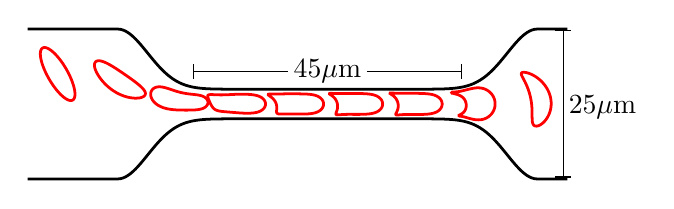
\begin{tikzpicture}[scale=1.0]

\begin{axis}[
  hide axis,
  axis equal image,
  xmin = -50,
  xmax = 40,
  ymin = -13,
  ymax = 13,
  xtick = \empty,
  ytick = \empty,
]


\addplot[black,line width=1pt] coordinates{
(1.0000e+02,0.0000e+00)
(1.0000e+02,4.3979e-01)
(1.0000e+02,8.7957e-01)
(1.0000e+02,1.3193e+00)
(1.0000e+02,1.7591e+00)
(1.0000e+02,2.1989e+00)
(1.0000e+02,2.6387e+00)
(1.0000e+02,3.0785e+00)
(1.0000e+02,3.5183e+00)
(9.9999e+01,3.9580e+00)
(9.9997e+01,4.3978e+00)
(9.9994e+01,4.8376e+00)
(9.9987e+01,5.2773e+00)
(9.9976e+01,5.7170e+00)
(9.9957e+01,6.1563e+00)
(9.9925e+01,6.5949e+00)
(9.9874e+01,7.0317e+00)
(9.9796e+01,7.4645e+00)
(9.9682e+01,7.8889e+00)
(9.9521e+01,8.2978e+00)
(9.9307e+01,8.6816e+00)
(9.9040e+01,9.0311e+00)
(9.8729e+01,9.3413e+00)
(9.8383e+01,9.6123e+00)
(9.8012e+01,9.8479e+00)
(9.7623e+01,1.0053e+01)
(9.7222e+01,1.0233e+01)
(9.6812e+01,1.0393e+01)
(9.6396e+01,1.0535e+01)
(9.5975e+01,1.0662e+01)
(9.5550e+01,1.0777e+01)
(9.5123e+01,1.0881e+01)
(9.4694e+01,1.0976e+01)
(9.4263e+01,1.1064e+01)
(9.3830e+01,1.1144e+01)
(9.3397e+01,1.1219e+01)
(9.2963e+01,1.1288e+01)
(9.2528e+01,1.1352e+01)
(9.2092e+01,1.1412e+01)
(9.1656e+01,1.1468e+01)
(9.1219e+01,1.1521e+01)
(9.0782e+01,1.1570e+01)
(9.0345e+01,1.1616e+01)
(8.9907e+01,1.1660e+01)
(8.9469e+01,1.1701e+01)
(8.9031e+01,1.1740e+01)
(8.8593e+01,1.1776e+01)
(8.8155e+01,1.1811e+01)
(8.7716e+01,1.1844e+01)
(8.7277e+01,1.1875e+01)
(8.6839e+01,1.1904e+01)
(8.6400e+01,1.1932e+01)
(8.5961e+01,1.1959e+01)
(8.5522e+01,1.1984e+01)
(8.5082e+01,1.2008e+01)
(8.4643e+01,1.2031e+01)
(8.4204e+01,1.2053e+01)
(8.3765e+01,1.2074e+01)
(8.3325e+01,1.2094e+01)
(8.2886e+01,1.2112e+01)
(8.2447e+01,1.2130e+01)
(8.2007e+01,1.2147e+01)
(8.1568e+01,1.2164e+01)
(8.1128e+01,1.2179e+01)
(8.0689e+01,1.2194e+01)
(8.0249e+01,1.2209e+01)
(7.9810e+01,1.2222e+01)
(7.9370e+01,1.2235e+01)
(7.8930e+01,1.2247e+01)
(7.8491e+01,1.2259e+01)
(7.8051e+01,1.2271e+01)
(7.7611e+01,1.2281e+01)
(7.7172e+01,1.2292e+01)
(7.6732e+01,1.2302e+01)
(7.6292e+01,1.2311e+01)
(7.5853e+01,1.2320e+01)
(7.5413e+01,1.2329e+01)
(7.4973e+01,1.2337e+01)
(7.4534e+01,1.2345e+01)
(7.4094e+01,1.2352e+01)
(7.3654e+01,1.2359e+01)
(7.3214e+01,1.2366e+01)
(7.2775e+01,1.2373e+01)
(7.2335e+01,1.2379e+01)
(7.1895e+01,1.2385e+01)
(7.1456e+01,1.2391e+01)
(7.1016e+01,1.2396e+01)
(7.0576e+01,1.2401e+01)
(7.0136e+01,1.2406e+01)
(6.9697e+01,1.2411e+01)
(6.9257e+01,1.2415e+01)
(6.8817e+01,1.2420e+01)
(6.8377e+01,1.2424e+01)
(6.7937e+01,1.2428e+01)
(6.7498e+01,1.2431e+01)
(6.7058e+01,1.2435e+01)
(6.6618e+01,1.2438e+01)
(6.6178e+01,1.2442e+01)
(6.5739e+01,1.2445e+01)
(6.5299e+01,1.2448e+01)
(6.4859e+01,1.2450e+01)
(6.4419e+01,1.2453e+01)
(6.3980e+01,1.2456e+01)
(6.3540e+01,1.2458e+01)
(6.3100e+01,1.2460e+01)
(6.2660e+01,1.2462e+01)
(6.2220e+01,1.2465e+01)
(6.1781e+01,1.2467e+01)
(6.1341e+01,1.2468e+01)
(6.0901e+01,1.2470e+01)
(6.0461e+01,1.2472e+01)
(6.0021e+01,1.2473e+01)
(5.9582e+01,1.2475e+01)
(5.9142e+01,1.2476e+01)
(5.8702e+01,1.2478e+01)
(5.8262e+01,1.2479e+01)
(5.7823e+01,1.2480e+01)
(5.7383e+01,1.2482e+01)
(5.6943e+01,1.2483e+01)
(5.6503e+01,1.2484e+01)
(5.6064e+01,1.2485e+01)
(5.5624e+01,1.2486e+01)
(5.5184e+01,1.2487e+01)
(5.4744e+01,1.2487e+01)
(5.4304e+01,1.2488e+01)
(5.3865e+01,1.2489e+01)
(5.3425e+01,1.2490e+01)
(5.2985e+01,1.2490e+01)
(5.2545e+01,1.2491e+01)
(5.2105e+01,1.2491e+01)
(5.1666e+01,1.2492e+01)
(5.1226e+01,1.2493e+01)
(5.0786e+01,1.2493e+01)
(5.0346e+01,1.2494e+01)
(4.9907e+01,1.2494e+01)
(4.9467e+01,1.2494e+01)
(4.9027e+01,1.2495e+01)
(4.8587e+01,1.2495e+01)
(4.8147e+01,1.2495e+01)
(4.7708e+01,1.2496e+01)
(4.7268e+01,1.2496e+01)
(4.6828e+01,1.2496e+01)
(4.6388e+01,1.2497e+01)
(4.5948e+01,1.2497e+01)
(4.5509e+01,1.2497e+01)
(4.5069e+01,1.2497e+01)
(4.4629e+01,1.2498e+01)
(4.4189e+01,1.2498e+01)
(4.3750e+01,1.2498e+01)
(4.3310e+01,1.2498e+01)
(4.2870e+01,1.2498e+01)
(4.2430e+01,1.2498e+01)
(4.1991e+01,1.2498e+01)
(4.1551e+01,1.2499e+01)
(4.1111e+01,1.2499e+01)
(4.0671e+01,1.2499e+01)
(4.0231e+01,1.2499e+01)
(3.9791e+01,1.2499e+01)
(3.9352e+01,1.2499e+01)
(3.8912e+01,1.2499e+01)
(3.8472e+01,1.2499e+01)
(3.8033e+01,1.2499e+01)
(3.7593e+01,1.2499e+01)
(3.7153e+01,1.2499e+01)
(3.6713e+01,1.2499e+01)
(3.6273e+01,1.2500e+01)
(3.5833e+01,1.2500e+01)
(3.5394e+01,1.2500e+01)
(3.4954e+01,1.2499e+01)
(3.4517e+01,1.2453e+01)
(3.4093e+01,1.2335e+01)
(3.3691e+01,1.2159e+01)
(3.3311e+01,1.1939e+01)
(3.2951e+01,1.1685e+01)
(3.2610e+01,1.1407e+01)
(3.2284e+01,1.1112e+01)
(3.1972e+01,1.0803e+01)
(3.1669e+01,1.0484e+01)
(3.1374e+01,1.0157e+01)
(3.1086e+01,9.8251e+00)
(3.0803e+01,9.4890e+00)
(3.0523e+01,9.1500e+00)
(3.0245e+01,8.8089e+00)
(2.9968e+01,8.4668e+00)
(2.9692e+01,8.1250e+00)
(2.9414e+01,7.7842e+00)
(2.9134e+01,7.4450e+00)
(2.8852e+01,7.1080e+00)
(2.8565e+01,6.7743e+00)
(2.8273e+01,6.4450e+00)
(2.7976e+01,6.1211e+00)
(2.7672e+01,5.8034e+00)
(2.7360e+01,5.4930e+00)
(2.7040e+01,5.1916e+00)
(2.6710e+01,4.9010e+00)
(2.6370e+01,4.6222e+00)
(2.6019e+01,4.3571e+00)
(2.5657e+01,4.1077e+00)
(2.5284e+01,3.8757e+00)
(2.4899e+01,3.6625e+00)
(2.4504e+01,3.4693e+00)
(2.4099e+01,3.2971e+00)
(2.3686e+01,3.1460e+00)
(2.3266e+01,3.0155e+00)
(2.2841e+01,2.9048e+00)
(2.2411e+01,2.8122e+00)
(2.1978e+01,2.7360e+00)
(2.1542e+01,2.6743e+00)
(2.1105e+01,2.6250e+00)
(2.0667e+01,2.5861e+00)
(2.0229e+01,2.5559e+00)
(1.9790e+01,2.5328e+00)
(1.9350e+01,2.5153e+00)
(1.8910e+01,2.5022e+00)
(1.8471e+01,2.4926e+00)
(1.8031e+01,2.4857e+00)
(1.7591e+01,2.4807e+00)
(1.7152e+01,2.4772e+00)
(1.6712e+01,2.4748e+00)
(1.6272e+01,2.4731e+00)
(1.5832e+01,2.4720e+00)
(1.5392e+01,2.4713e+00)
(1.4953e+01,2.4708e+00)
(1.4513e+01,2.4705e+00)
(1.4073e+01,2.4703e+00)
(1.3633e+01,2.4702e+00)
(1.3193e+01,2.4701e+00)
(1.2754e+01,2.4701e+00)
(1.2314e+01,2.4701e+00)
(1.1874e+01,2.4701e+00)
(1.1434e+01,2.4701e+00)
(1.0995e+01,2.4701e+00)
(1.0555e+01,2.4701e+00)
(1.0115e+01,2.4701e+00)
(9.6752e+00,2.4701e+00)
(9.2354e+00,2.4701e+00)
(8.7956e+00,2.4701e+00)
(8.3559e+00,2.4701e+00)
(7.9161e+00,2.4701e+00)
(7.4763e+00,2.4701e+00)
(7.0365e+00,2.4701e+00)
(6.5967e+00,2.4701e+00)
(6.1570e+00,2.4701e+00)
(5.7172e+00,2.4701e+00)
(5.2774e+00,2.4701e+00)
(4.8376e+00,2.4701e+00)
(4.3978e+00,2.4701e+00)
(3.9580e+00,2.4701e+00)
(3.5183e+00,2.4701e+00)
(3.0785e+00,2.4701e+00)
(2.6387e+00,2.4701e+00)
(2.1989e+00,2.4701e+00)
(1.7591e+00,2.4701e+00)
(1.3193e+00,2.4701e+00)
(8.7959e-01,2.4701e+00)
(4.3976e-01,2.4701e+00)
(-3.8286e-14,2.4701e+00)
(-4.3976e-01,2.4701e+00)
(-8.7959e-01,2.4701e+00)
(-1.3193e+00,2.4701e+00)
(-1.7591e+00,2.4701e+00)
(-2.1989e+00,2.4701e+00)
(-2.6387e+00,2.4701e+00)
(-3.0785e+00,2.4701e+00)
(-3.5183e+00,2.4701e+00)
(-3.9580e+00,2.4701e+00)
(-4.3978e+00,2.4701e+00)
(-4.8376e+00,2.4701e+00)
(-5.2774e+00,2.4701e+00)
(-5.7172e+00,2.4701e+00)
(-6.1570e+00,2.4701e+00)
(-6.5967e+00,2.4701e+00)
(-7.0365e+00,2.4701e+00)
(-7.4763e+00,2.4701e+00)
(-7.9161e+00,2.4701e+00)
(-8.3559e+00,2.4701e+00)
(-8.7956e+00,2.4701e+00)
(-9.2354e+00,2.4701e+00)
(-9.6752e+00,2.4701e+00)
(-1.0115e+01,2.4701e+00)
(-1.0555e+01,2.4701e+00)
(-1.0995e+01,2.4701e+00)
(-1.1434e+01,2.4701e+00)
(-1.1874e+01,2.4701e+00)
(-1.2314e+01,2.4701e+00)
(-1.2754e+01,2.4701e+00)
(-1.3193e+01,2.4701e+00)
(-1.3633e+01,2.4702e+00)
(-1.4073e+01,2.4703e+00)
(-1.4513e+01,2.4705e+00)
(-1.4953e+01,2.4708e+00)
(-1.5392e+01,2.4713e+00)
(-1.5832e+01,2.4720e+00)
(-1.6272e+01,2.4731e+00)
(-1.6712e+01,2.4748e+00)
(-1.7152e+01,2.4772e+00)
(-1.7591e+01,2.4807e+00)
(-1.8031e+01,2.4857e+00)
(-1.8471e+01,2.4926e+00)
(-1.8910e+01,2.5022e+00)
(-1.9350e+01,2.5153e+00)
(-1.9790e+01,2.5328e+00)
(-2.0229e+01,2.5559e+00)
(-2.0667e+01,2.5861e+00)
(-2.1105e+01,2.6250e+00)
(-2.1542e+01,2.6743e+00)
(-2.1978e+01,2.7360e+00)
(-2.2411e+01,2.8122e+00)
(-2.2841e+01,2.9048e+00)
(-2.3266e+01,3.0155e+00)
(-2.3686e+01,3.1460e+00)
(-2.4099e+01,3.2971e+00)
(-2.4504e+01,3.4693e+00)
(-2.4899e+01,3.6625e+00)
(-2.5284e+01,3.8757e+00)
(-2.5657e+01,4.1077e+00)
(-2.6019e+01,4.3571e+00)
(-2.6370e+01,4.6222e+00)
(-2.6710e+01,4.9010e+00)
(-2.7040e+01,5.1916e+00)
(-2.7360e+01,5.4930e+00)
(-2.7672e+01,5.8034e+00)
(-2.7976e+01,6.1211e+00)
(-2.8273e+01,6.4450e+00)
(-2.8565e+01,6.7743e+00)
(-2.8852e+01,7.1080e+00)
(-2.9134e+01,7.4450e+00)
(-2.9414e+01,7.7842e+00)
(-2.9692e+01,8.1250e+00)
(-2.9968e+01,8.4668e+00)
(-3.0245e+01,8.8089e+00)
(-3.0523e+01,9.1500e+00)
(-3.0803e+01,9.4890e+00)
(-3.1086e+01,9.8251e+00)
(-3.1374e+01,1.0157e+01)
(-3.1669e+01,1.0484e+01)
(-3.1972e+01,1.0803e+01)
(-3.2284e+01,1.1112e+01)
(-3.2610e+01,1.1407e+01)
(-3.2951e+01,1.1685e+01)
(-3.3311e+01,1.1939e+01)
(-3.3691e+01,1.2159e+01)
(-3.4093e+01,1.2335e+01)
(-3.4517e+01,1.2453e+01)
(-3.4954e+01,1.2499e+01)
(-3.5394e+01,1.2500e+01)
(-3.5833e+01,1.2500e+01)
(-3.6273e+01,1.2500e+01)
(-3.6713e+01,1.2499e+01)
(-3.7153e+01,1.2499e+01)
(-3.7593e+01,1.2499e+01)
(-3.8033e+01,1.2499e+01)
(-3.8472e+01,1.2499e+01)
(-3.8912e+01,1.2499e+01)
(-3.9352e+01,1.2499e+01)
(-3.9791e+01,1.2499e+01)
(-4.0231e+01,1.2499e+01)
(-4.0671e+01,1.2499e+01)
(-4.1111e+01,1.2499e+01)
(-4.1551e+01,1.2499e+01)
(-4.1991e+01,1.2498e+01)
(-4.2430e+01,1.2498e+01)
(-4.2870e+01,1.2498e+01)
(-4.3310e+01,1.2498e+01)
(-4.3750e+01,1.2498e+01)
(-4.4189e+01,1.2498e+01)
(-4.4629e+01,1.2498e+01)
(-4.5069e+01,1.2497e+01)
(-4.5509e+01,1.2497e+01)
(-4.5948e+01,1.2497e+01)
(-4.6388e+01,1.2497e+01)
(-4.6828e+01,1.2496e+01)
(-4.7268e+01,1.2496e+01)
(-4.7708e+01,1.2496e+01)
(-4.8147e+01,1.2495e+01)
(-4.8587e+01,1.2495e+01)
(-4.9027e+01,1.2495e+01)
(-4.9467e+01,1.2494e+01)
(-4.9907e+01,1.2494e+01)
(-5.0346e+01,1.2494e+01)
(-5.0786e+01,1.2493e+01)
(-5.1226e+01,1.2493e+01)
(-5.1666e+01,1.2492e+01)
(-5.2105e+01,1.2491e+01)
(-5.2545e+01,1.2491e+01)
(-5.2985e+01,1.2490e+01)
(-5.3425e+01,1.2490e+01)
(-5.3865e+01,1.2489e+01)
(-5.4304e+01,1.2488e+01)
(-5.4744e+01,1.2487e+01)
(-5.5184e+01,1.2487e+01)
(-5.5624e+01,1.2486e+01)
(-5.6064e+01,1.2485e+01)
(-5.6503e+01,1.2484e+01)
(-5.6943e+01,1.2483e+01)
(-5.7383e+01,1.2482e+01)
(-5.7823e+01,1.2480e+01)
(-5.8262e+01,1.2479e+01)
(-5.8702e+01,1.2478e+01)
(-5.9142e+01,1.2476e+01)
(-5.9582e+01,1.2475e+01)
(-6.0021e+01,1.2473e+01)
(-6.0461e+01,1.2472e+01)
(-6.0901e+01,1.2470e+01)
(-6.1341e+01,1.2468e+01)
(-6.1781e+01,1.2467e+01)
(-6.2220e+01,1.2465e+01)
(-6.2660e+01,1.2462e+01)
(-6.3100e+01,1.2460e+01)
(-6.3540e+01,1.2458e+01)
(-6.3980e+01,1.2456e+01)
(-6.4419e+01,1.2453e+01)
(-6.4859e+01,1.2450e+01)
(-6.5299e+01,1.2448e+01)
(-6.5739e+01,1.2445e+01)
(-6.6178e+01,1.2442e+01)
(-6.6618e+01,1.2438e+01)
(-6.7058e+01,1.2435e+01)
(-6.7498e+01,1.2431e+01)
(-6.7937e+01,1.2428e+01)
(-6.8377e+01,1.2424e+01)
(-6.8817e+01,1.2420e+01)
(-6.9257e+01,1.2415e+01)
(-6.9697e+01,1.2411e+01)
(-7.0136e+01,1.2406e+01)
(-7.0576e+01,1.2401e+01)
(-7.1016e+01,1.2396e+01)
(-7.1456e+01,1.2391e+01)
(-7.1895e+01,1.2385e+01)
(-7.2335e+01,1.2379e+01)
(-7.2775e+01,1.2373e+01)
(-7.3214e+01,1.2366e+01)
(-7.3654e+01,1.2359e+01)
(-7.4094e+01,1.2352e+01)
(-7.4534e+01,1.2345e+01)
(-7.4973e+01,1.2337e+01)
(-7.5413e+01,1.2329e+01)
(-7.5853e+01,1.2320e+01)
(-7.6292e+01,1.2311e+01)
(-7.6732e+01,1.2302e+01)
(-7.7172e+01,1.2292e+01)
(-7.7611e+01,1.2281e+01)
(-7.8051e+01,1.2271e+01)
(-7.8491e+01,1.2259e+01)
(-7.8930e+01,1.2247e+01)
(-7.9370e+01,1.2235e+01)
(-7.9810e+01,1.2222e+01)
(-8.0249e+01,1.2209e+01)
(-8.0689e+01,1.2194e+01)
(-8.1128e+01,1.2179e+01)
(-8.1568e+01,1.2164e+01)
(-8.2007e+01,1.2147e+01)
(-8.2447e+01,1.2130e+01)
(-8.2886e+01,1.2112e+01)
(-8.3325e+01,1.2094e+01)
(-8.3765e+01,1.2074e+01)
(-8.4204e+01,1.2053e+01)
(-8.4643e+01,1.2031e+01)
(-8.5082e+01,1.2008e+01)
(-8.5522e+01,1.1984e+01)
(-8.5961e+01,1.1959e+01)
(-8.6400e+01,1.1932e+01)
(-8.6839e+01,1.1904e+01)
(-8.7277e+01,1.1875e+01)
(-8.7716e+01,1.1844e+01)
(-8.8155e+01,1.1811e+01)
(-8.8593e+01,1.1776e+01)
(-8.9031e+01,1.1740e+01)
(-8.9469e+01,1.1701e+01)
(-8.9907e+01,1.1660e+01)
(-9.0345e+01,1.1616e+01)
(-9.0782e+01,1.1570e+01)
(-9.1219e+01,1.1521e+01)
(-9.1656e+01,1.1468e+01)
(-9.2092e+01,1.1412e+01)
(-9.2528e+01,1.1352e+01)
(-9.2963e+01,1.1288e+01)
(-9.3397e+01,1.1219e+01)
(-9.3830e+01,1.1144e+01)
(-9.4263e+01,1.1064e+01)
(-9.4694e+01,1.0976e+01)
(-9.5123e+01,1.0881e+01)
(-9.5550e+01,1.0777e+01)
(-9.5975e+01,1.0662e+01)
(-9.6396e+01,1.0535e+01)
(-9.6812e+01,1.0393e+01)
(-9.7222e+01,1.0233e+01)
(-9.7623e+01,1.0053e+01)
(-9.8012e+01,9.8479e+00)
(-9.8383e+01,9.6123e+00)
(-9.8729e+01,9.3413e+00)
(-9.9040e+01,9.0311e+00)
(-9.9307e+01,8.6816e+00)
(-9.9521e+01,8.2978e+00)
(-9.9682e+01,7.8889e+00)
(-9.9796e+01,7.4645e+00)
(-9.9874e+01,7.0317e+00)
(-9.9925e+01,6.5949e+00)
(-9.9957e+01,6.1563e+00)
(-9.9976e+01,5.7170e+00)
(-9.9987e+01,5.2773e+00)
(-9.9994e+01,4.8376e+00)
(-9.9997e+01,4.3978e+00)
(-9.9999e+01,3.9580e+00)
(-1.0000e+02,3.5183e+00)
(-1.0000e+02,3.0785e+00)
(-1.0000e+02,2.6387e+00)
(-1.0000e+02,2.1989e+00)
(-1.0000e+02,1.7591e+00)
(-1.0000e+02,1.3193e+00)
(-1.0000e+02,8.7957e-01)
(-1.0000e+02,4.3979e-01)
(-1.0000e+02,-4.0203e-15)
(-1.0000e+02,-4.3979e-01)
(-1.0000e+02,-8.7957e-01)
(-1.0000e+02,-1.3193e+00)
(-1.0000e+02,-1.7591e+00)
(-1.0000e+02,-2.1989e+00)
(-1.0000e+02,-2.6387e+00)
(-1.0000e+02,-3.0785e+00)
(-1.0000e+02,-3.5183e+00)
(-9.9999e+01,-3.9580e+00)
(-9.9997e+01,-4.3978e+00)
(-9.9994e+01,-4.8376e+00)
(-9.9987e+01,-5.2773e+00)
(-9.9976e+01,-5.7170e+00)
(-9.9957e+01,-6.1563e+00)
(-9.9925e+01,-6.5949e+00)
(-9.9874e+01,-7.0317e+00)
(-9.9796e+01,-7.4645e+00)
(-9.9682e+01,-7.8889e+00)
(-9.9521e+01,-8.2978e+00)
(-9.9307e+01,-8.6816e+00)
(-9.9040e+01,-9.0311e+00)
(-9.8729e+01,-9.3413e+00)
(-9.8383e+01,-9.6123e+00)
(-9.8012e+01,-9.8479e+00)
(-9.7623e+01,-1.0053e+01)
(-9.7222e+01,-1.0233e+01)
(-9.6812e+01,-1.0393e+01)
(-9.6396e+01,-1.0535e+01)
(-9.5975e+01,-1.0662e+01)
(-9.5550e+01,-1.0777e+01)
(-9.5123e+01,-1.0881e+01)
(-9.4694e+01,-1.0976e+01)
(-9.4263e+01,-1.1064e+01)
(-9.3830e+01,-1.1144e+01)
(-9.3397e+01,-1.1219e+01)
(-9.2963e+01,-1.1288e+01)
(-9.2528e+01,-1.1352e+01)
(-9.2092e+01,-1.1412e+01)
(-9.1656e+01,-1.1468e+01)
(-9.1219e+01,-1.1521e+01)
(-9.0782e+01,-1.1570e+01)
(-9.0345e+01,-1.1616e+01)
(-8.9907e+01,-1.1660e+01)
(-8.9469e+01,-1.1701e+01)
(-8.9031e+01,-1.1740e+01)
(-8.8593e+01,-1.1776e+01)
(-8.8155e+01,-1.1811e+01)
(-8.7716e+01,-1.1844e+01)
(-8.7277e+01,-1.1875e+01)
(-8.6839e+01,-1.1904e+01)
(-8.6400e+01,-1.1932e+01)
(-8.5961e+01,-1.1959e+01)
(-8.5522e+01,-1.1984e+01)
(-8.5082e+01,-1.2008e+01)
(-8.4643e+01,-1.2031e+01)
(-8.4204e+01,-1.2053e+01)
(-8.3765e+01,-1.2074e+01)
(-8.3325e+01,-1.2094e+01)
(-8.2886e+01,-1.2112e+01)
(-8.2447e+01,-1.2130e+01)
(-8.2007e+01,-1.2147e+01)
(-8.1568e+01,-1.2164e+01)
(-8.1128e+01,-1.2179e+01)
(-8.0689e+01,-1.2194e+01)
(-8.0249e+01,-1.2209e+01)
(-7.9810e+01,-1.2222e+01)
(-7.9370e+01,-1.2235e+01)
(-7.8930e+01,-1.2247e+01)
(-7.8491e+01,-1.2259e+01)
(-7.8051e+01,-1.2271e+01)
(-7.7611e+01,-1.2281e+01)
(-7.7172e+01,-1.2292e+01)
(-7.6732e+01,-1.2302e+01)
(-7.6292e+01,-1.2311e+01)
(-7.5853e+01,-1.2320e+01)
(-7.5413e+01,-1.2329e+01)
(-7.4973e+01,-1.2337e+01)
(-7.4534e+01,-1.2345e+01)
(-7.4094e+01,-1.2352e+01)
(-7.3654e+01,-1.2359e+01)
(-7.3214e+01,-1.2366e+01)
(-7.2775e+01,-1.2373e+01)
(-7.2335e+01,-1.2379e+01)
(-7.1895e+01,-1.2385e+01)
(-7.1456e+01,-1.2391e+01)
(-7.1016e+01,-1.2396e+01)
(-7.0576e+01,-1.2401e+01)
(-7.0136e+01,-1.2406e+01)
(-6.9697e+01,-1.2411e+01)
(-6.9257e+01,-1.2415e+01)
(-6.8817e+01,-1.2420e+01)
(-6.8377e+01,-1.2424e+01)
(-6.7937e+01,-1.2428e+01)
(-6.7498e+01,-1.2431e+01)
(-6.7058e+01,-1.2435e+01)
(-6.6618e+01,-1.2438e+01)
(-6.6178e+01,-1.2442e+01)
(-6.5739e+01,-1.2445e+01)
(-6.5299e+01,-1.2448e+01)
(-6.4859e+01,-1.2450e+01)
(-6.4419e+01,-1.2453e+01)
(-6.3980e+01,-1.2456e+01)
(-6.3540e+01,-1.2458e+01)
(-6.3100e+01,-1.2460e+01)
(-6.2660e+01,-1.2462e+01)
(-6.2220e+01,-1.2465e+01)
(-6.1781e+01,-1.2467e+01)
(-6.1341e+01,-1.2468e+01)
(-6.0901e+01,-1.2470e+01)
(-6.0461e+01,-1.2472e+01)
(-6.0021e+01,-1.2473e+01)
(-5.9582e+01,-1.2475e+01)
(-5.9142e+01,-1.2476e+01)
(-5.8702e+01,-1.2478e+01)
(-5.8262e+01,-1.2479e+01)
(-5.7823e+01,-1.2480e+01)
(-5.7383e+01,-1.2482e+01)
(-5.6943e+01,-1.2483e+01)
(-5.6503e+01,-1.2484e+01)
(-5.6064e+01,-1.2485e+01)
(-5.5624e+01,-1.2486e+01)
(-5.5184e+01,-1.2487e+01)
(-5.4744e+01,-1.2487e+01)
(-5.4304e+01,-1.2488e+01)
(-5.3865e+01,-1.2489e+01)
(-5.3425e+01,-1.2490e+01)
(-5.2985e+01,-1.2490e+01)
(-5.2545e+01,-1.2491e+01)
(-5.2105e+01,-1.2491e+01)
(-5.1666e+01,-1.2492e+01)
(-5.1226e+01,-1.2493e+01)
(-5.0786e+01,-1.2493e+01)
(-5.0346e+01,-1.2494e+01)
(-4.9907e+01,-1.2494e+01)
(-4.9467e+01,-1.2494e+01)
(-4.9027e+01,-1.2495e+01)
(-4.8587e+01,-1.2495e+01)
(-4.8147e+01,-1.2495e+01)
(-4.7708e+01,-1.2496e+01)
(-4.7268e+01,-1.2496e+01)
(-4.6828e+01,-1.2496e+01)
(-4.6388e+01,-1.2497e+01)
(-4.5948e+01,-1.2497e+01)
(-4.5509e+01,-1.2497e+01)
(-4.5069e+01,-1.2497e+01)
(-4.4629e+01,-1.2498e+01)
(-4.4189e+01,-1.2498e+01)
(-4.3750e+01,-1.2498e+01)
(-4.3310e+01,-1.2498e+01)
(-4.2870e+01,-1.2498e+01)
(-4.2430e+01,-1.2498e+01)
(-4.1991e+01,-1.2498e+01)
(-4.1551e+01,-1.2499e+01)
(-4.1111e+01,-1.2499e+01)
(-4.0671e+01,-1.2499e+01)
(-4.0231e+01,-1.2499e+01)
(-3.9791e+01,-1.2499e+01)
(-3.9352e+01,-1.2499e+01)
(-3.8912e+01,-1.2499e+01)
(-3.8472e+01,-1.2499e+01)
(-3.8033e+01,-1.2499e+01)
(-3.7593e+01,-1.2499e+01)
(-3.7153e+01,-1.2499e+01)
(-3.6713e+01,-1.2499e+01)
(-3.6273e+01,-1.2500e+01)
(-3.5833e+01,-1.2500e+01)
(-3.5394e+01,-1.2500e+01)
(-3.4954e+01,-1.2499e+01)
(-3.4517e+01,-1.2453e+01)
(-3.4093e+01,-1.2335e+01)
(-3.3691e+01,-1.2159e+01)
(-3.3311e+01,-1.1939e+01)
(-3.2951e+01,-1.1685e+01)
(-3.2610e+01,-1.1407e+01)
(-3.2284e+01,-1.1112e+01)
(-3.1972e+01,-1.0803e+01)
(-3.1669e+01,-1.0484e+01)
(-3.1374e+01,-1.0157e+01)
(-3.1086e+01,-9.8251e+00)
(-3.0803e+01,-9.4890e+00)
(-3.0523e+01,-9.1500e+00)
(-3.0245e+01,-8.8089e+00)
(-2.9968e+01,-8.4668e+00)
(-2.9692e+01,-8.1250e+00)
(-2.9414e+01,-7.7842e+00)
(-2.9134e+01,-7.4450e+00)
(-2.8852e+01,-7.1080e+00)
(-2.8565e+01,-6.7743e+00)
(-2.8273e+01,-6.4450e+00)
(-2.7976e+01,-6.1211e+00)
(-2.7672e+01,-5.8034e+00)
(-2.7360e+01,-5.4930e+00)
(-2.7040e+01,-5.1916e+00)
(-2.6710e+01,-4.9010e+00)
(-2.6370e+01,-4.6222e+00)
(-2.6019e+01,-4.3571e+00)
(-2.5657e+01,-4.1077e+00)
(-2.5284e+01,-3.8757e+00)
(-2.4899e+01,-3.6625e+00)
(-2.4504e+01,-3.4693e+00)
(-2.4099e+01,-3.2971e+00)
(-2.3686e+01,-3.1460e+00)
(-2.3266e+01,-3.0155e+00)
(-2.2841e+01,-2.9048e+00)
(-2.2411e+01,-2.8122e+00)
(-2.1978e+01,-2.7360e+00)
(-2.1542e+01,-2.6743e+00)
(-2.1105e+01,-2.6250e+00)
(-2.0667e+01,-2.5861e+00)
(-2.0229e+01,-2.5559e+00)
(-1.9790e+01,-2.5328e+00)
(-1.9350e+01,-2.5153e+00)
(-1.8910e+01,-2.5022e+00)
(-1.8471e+01,-2.4926e+00)
(-1.8031e+01,-2.4857e+00)
(-1.7591e+01,-2.4807e+00)
(-1.7152e+01,-2.4772e+00)
(-1.6712e+01,-2.4748e+00)
(-1.6272e+01,-2.4731e+00)
(-1.5832e+01,-2.4720e+00)
(-1.5392e+01,-2.4713e+00)
(-1.4953e+01,-2.4708e+00)
(-1.4513e+01,-2.4705e+00)
(-1.4073e+01,-2.4703e+00)
(-1.3633e+01,-2.4702e+00)
(-1.3193e+01,-2.4701e+00)
(-1.2754e+01,-2.4701e+00)
(-1.2314e+01,-2.4701e+00)
(-1.1874e+01,-2.4701e+00)
(-1.1434e+01,-2.4701e+00)
(-1.0995e+01,-2.4701e+00)
(-1.0555e+01,-2.4701e+00)
(-1.0115e+01,-2.4701e+00)
(-9.6752e+00,-2.4701e+00)
(-9.2354e+00,-2.4701e+00)
(-8.7956e+00,-2.4701e+00)
(-8.3559e+00,-2.4701e+00)
(-7.9161e+00,-2.4701e+00)
(-7.4763e+00,-2.4701e+00)
(-7.0365e+00,-2.4701e+00)
(-6.5967e+00,-2.4701e+00)
(-6.1570e+00,-2.4701e+00)
(-5.7172e+00,-2.4701e+00)
(-5.2774e+00,-2.4701e+00)
(-4.8376e+00,-2.4701e+00)
(-4.3978e+00,-2.4701e+00)
(-3.9580e+00,-2.4701e+00)
(-3.5183e+00,-2.4701e+00)
(-3.0785e+00,-2.4701e+00)
(-2.6387e+00,-2.4701e+00)
(-2.1989e+00,-2.4701e+00)
(-1.7591e+00,-2.4701e+00)
(-1.3193e+00,-2.4701e+00)
(-8.7959e-01,-2.4701e+00)
(-4.3976e-01,-2.4701e+00)
(7.0448e-14,-2.4701e+00)
(4.3976e-01,-2.4701e+00)
(8.7959e-01,-2.4701e+00)
(1.3193e+00,-2.4701e+00)
(1.7591e+00,-2.4701e+00)
(2.1989e+00,-2.4701e+00)
(2.6387e+00,-2.4701e+00)
(3.0785e+00,-2.4701e+00)
(3.5183e+00,-2.4701e+00)
(3.9580e+00,-2.4701e+00)
(4.3978e+00,-2.4701e+00)
(4.8376e+00,-2.4701e+00)
(5.2774e+00,-2.4701e+00)
(5.7172e+00,-2.4701e+00)
(6.1570e+00,-2.4701e+00)
(6.5967e+00,-2.4701e+00)
(7.0365e+00,-2.4701e+00)
(7.4763e+00,-2.4701e+00)
(7.9161e+00,-2.4701e+00)
(8.3559e+00,-2.4701e+00)
(8.7956e+00,-2.4701e+00)
(9.2354e+00,-2.4701e+00)
(9.6752e+00,-2.4701e+00)
(1.0115e+01,-2.4701e+00)
(1.0555e+01,-2.4701e+00)
(1.0995e+01,-2.4701e+00)
(1.1434e+01,-2.4701e+00)
(1.1874e+01,-2.4701e+00)
(1.2314e+01,-2.4701e+00)
(1.2754e+01,-2.4701e+00)
(1.3193e+01,-2.4701e+00)
(1.3633e+01,-2.4702e+00)
(1.4073e+01,-2.4703e+00)
(1.4513e+01,-2.4705e+00)
(1.4953e+01,-2.4708e+00)
(1.5392e+01,-2.4713e+00)
(1.5832e+01,-2.4720e+00)
(1.6272e+01,-2.4731e+00)
(1.6712e+01,-2.4748e+00)
(1.7152e+01,-2.4772e+00)
(1.7591e+01,-2.4807e+00)
(1.8031e+01,-2.4857e+00)
(1.8471e+01,-2.4926e+00)
(1.8910e+01,-2.5022e+00)
(1.9350e+01,-2.5153e+00)
(1.9790e+01,-2.5328e+00)
(2.0229e+01,-2.5559e+00)
(2.0667e+01,-2.5861e+00)
(2.1105e+01,-2.6250e+00)
(2.1542e+01,-2.6743e+00)
(2.1978e+01,-2.7360e+00)
(2.2411e+01,-2.8122e+00)
(2.2841e+01,-2.9048e+00)
(2.3266e+01,-3.0155e+00)
(2.3686e+01,-3.1460e+00)
(2.4099e+01,-3.2971e+00)
(2.4504e+01,-3.4693e+00)
(2.4899e+01,-3.6625e+00)
(2.5284e+01,-3.8757e+00)
(2.5657e+01,-4.1077e+00)
(2.6019e+01,-4.3571e+00)
(2.6370e+01,-4.6222e+00)
(2.6710e+01,-4.9010e+00)
(2.7040e+01,-5.1916e+00)
(2.7360e+01,-5.4930e+00)
(2.7672e+01,-5.8034e+00)
(2.7976e+01,-6.1211e+00)
(2.8273e+01,-6.4450e+00)
(2.8565e+01,-6.7743e+00)
(2.8852e+01,-7.1080e+00)
(2.9134e+01,-7.4450e+00)
(2.9414e+01,-7.7842e+00)
(2.9692e+01,-8.1250e+00)
(2.9968e+01,-8.4668e+00)
(3.0245e+01,-8.8089e+00)
(3.0523e+01,-9.1500e+00)
(3.0803e+01,-9.4890e+00)
(3.1086e+01,-9.8251e+00)
(3.1374e+01,-1.0157e+01)
(3.1669e+01,-1.0484e+01)
(3.1972e+01,-1.0803e+01)
(3.2284e+01,-1.1112e+01)
(3.2610e+01,-1.1407e+01)
(3.2951e+01,-1.1685e+01)
(3.3311e+01,-1.1939e+01)
(3.3691e+01,-1.2159e+01)
(3.4093e+01,-1.2335e+01)
(3.4517e+01,-1.2453e+01)
(3.4954e+01,-1.2499e+01)
(3.5394e+01,-1.2500e+01)
(3.5833e+01,-1.2500e+01)
(3.6273e+01,-1.2500e+01)
(3.6713e+01,-1.2499e+01)
(3.7153e+01,-1.2499e+01)
(3.7593e+01,-1.2499e+01)
(3.8033e+01,-1.2499e+01)
(3.8472e+01,-1.2499e+01)
(3.8912e+01,-1.2499e+01)
(3.9352e+01,-1.2499e+01)
(3.9791e+01,-1.2499e+01)
(4.0231e+01,-1.2499e+01)
(4.0671e+01,-1.2499e+01)
(4.1111e+01,-1.2499e+01)
(4.1551e+01,-1.2499e+01)
(4.1991e+01,-1.2498e+01)
(4.2430e+01,-1.2498e+01)
(4.2870e+01,-1.2498e+01)
(4.3310e+01,-1.2498e+01)
(4.3750e+01,-1.2498e+01)
(4.4189e+01,-1.2498e+01)
(4.4629e+01,-1.2498e+01)
(4.5069e+01,-1.2497e+01)
(4.5509e+01,-1.2497e+01)
(4.5948e+01,-1.2497e+01)
(4.6388e+01,-1.2497e+01)
(4.6828e+01,-1.2496e+01)
(4.7268e+01,-1.2496e+01)
(4.7708e+01,-1.2496e+01)
(4.8147e+01,-1.2495e+01)
(4.8587e+01,-1.2495e+01)
(4.9027e+01,-1.2495e+01)
(4.9467e+01,-1.2494e+01)
(4.9907e+01,-1.2494e+01)
(5.0346e+01,-1.2494e+01)
(5.0786e+01,-1.2493e+01)
(5.1226e+01,-1.2493e+01)
(5.1666e+01,-1.2492e+01)
(5.2105e+01,-1.2491e+01)
(5.2545e+01,-1.2491e+01)
(5.2985e+01,-1.2490e+01)
(5.3425e+01,-1.2490e+01)
(5.3865e+01,-1.2489e+01)
(5.4304e+01,-1.2488e+01)
(5.4744e+01,-1.2487e+01)
(5.5184e+01,-1.2487e+01)
(5.5624e+01,-1.2486e+01)
(5.6064e+01,-1.2485e+01)
(5.6503e+01,-1.2484e+01)
(5.6943e+01,-1.2483e+01)
(5.7383e+01,-1.2482e+01)
(5.7823e+01,-1.2480e+01)
(5.8262e+01,-1.2479e+01)
(5.8702e+01,-1.2478e+01)
(5.9142e+01,-1.2476e+01)
(5.9582e+01,-1.2475e+01)
(6.0021e+01,-1.2473e+01)
(6.0461e+01,-1.2472e+01)
(6.0901e+01,-1.2470e+01)
(6.1341e+01,-1.2468e+01)
(6.1781e+01,-1.2467e+01)
(6.2220e+01,-1.2465e+01)
(6.2660e+01,-1.2462e+01)
(6.3100e+01,-1.2460e+01)
(6.3540e+01,-1.2458e+01)
(6.3980e+01,-1.2456e+01)
(6.4419e+01,-1.2453e+01)
(6.4859e+01,-1.2450e+01)
(6.5299e+01,-1.2448e+01)
(6.5739e+01,-1.2445e+01)
(6.6178e+01,-1.2442e+01)
(6.6618e+01,-1.2438e+01)
(6.7058e+01,-1.2435e+01)
(6.7498e+01,-1.2431e+01)
(6.7937e+01,-1.2428e+01)
(6.8377e+01,-1.2424e+01)
(6.8817e+01,-1.2420e+01)
(6.9257e+01,-1.2415e+01)
(6.9697e+01,-1.2411e+01)
(7.0136e+01,-1.2406e+01)
(7.0576e+01,-1.2401e+01)
(7.1016e+01,-1.2396e+01)
(7.1456e+01,-1.2391e+01)
(7.1895e+01,-1.2385e+01)
(7.2335e+01,-1.2379e+01)
(7.2775e+01,-1.2373e+01)
(7.3214e+01,-1.2366e+01)
(7.3654e+01,-1.2359e+01)
(7.4094e+01,-1.2352e+01)
(7.4534e+01,-1.2345e+01)
(7.4973e+01,-1.2337e+01)
(7.5413e+01,-1.2329e+01)
(7.5853e+01,-1.2320e+01)
(7.6292e+01,-1.2311e+01)
(7.6732e+01,-1.2302e+01)
(7.7172e+01,-1.2292e+01)
(7.7611e+01,-1.2281e+01)
(7.8051e+01,-1.2271e+01)
(7.8491e+01,-1.2259e+01)
(7.8930e+01,-1.2247e+01)
(7.9370e+01,-1.2235e+01)
(7.9810e+01,-1.2222e+01)
(8.0249e+01,-1.2209e+01)
(8.0689e+01,-1.2194e+01)
(8.1128e+01,-1.2179e+01)
(8.1568e+01,-1.2164e+01)
(8.2007e+01,-1.2147e+01)
(8.2447e+01,-1.2130e+01)
(8.2886e+01,-1.2112e+01)
(8.3325e+01,-1.2094e+01)
(8.3765e+01,-1.2074e+01)
(8.4204e+01,-1.2053e+01)
(8.4643e+01,-1.2031e+01)
(8.5082e+01,-1.2008e+01)
(8.5522e+01,-1.1984e+01)
(8.5961e+01,-1.1959e+01)
(8.6400e+01,-1.1932e+01)
(8.6839e+01,-1.1904e+01)
(8.7277e+01,-1.1875e+01)
(8.7716e+01,-1.1844e+01)
(8.8155e+01,-1.1811e+01)
(8.8593e+01,-1.1776e+01)
(8.9031e+01,-1.1740e+01)
(8.9469e+01,-1.1701e+01)
(8.9907e+01,-1.1660e+01)
(9.0345e+01,-1.1616e+01)
(9.0782e+01,-1.1570e+01)
(9.1219e+01,-1.1521e+01)
(9.1656e+01,-1.1468e+01)
(9.2092e+01,-1.1412e+01)
(9.2528e+01,-1.1352e+01)
(9.2963e+01,-1.1288e+01)
(9.3397e+01,-1.1219e+01)
(9.3830e+01,-1.1144e+01)
(9.4263e+01,-1.1064e+01)
(9.4694e+01,-1.0976e+01)
(9.5123e+01,-1.0881e+01)
(9.5550e+01,-1.0777e+01)
(9.5975e+01,-1.0662e+01)
(9.6396e+01,-1.0535e+01)
(9.6812e+01,-1.0393e+01)
(9.7222e+01,-1.0233e+01)
(9.7623e+01,-1.0053e+01)
(9.8012e+01,-9.8479e+00)
(9.8383e+01,-9.6123e+00)
(9.8729e+01,-9.3413e+00)
(9.9040e+01,-9.0311e+00)
(9.9307e+01,-8.6816e+00)
(9.9521e+01,-8.2978e+00)
(9.9682e+01,-7.8889e+00)
(9.9796e+01,-7.4645e+00)
(9.9874e+01,-7.0317e+00)
(9.9925e+01,-6.5949e+00)
(9.9957e+01,-6.1563e+00)
(9.9976e+01,-5.7170e+00)
(9.9987e+01,-5.2773e+00)
(9.9994e+01,-4.8376e+00)
(9.9997e+01,-4.3978e+00)
(9.9999e+01,-3.9580e+00)
(1.0000e+02,-3.5183e+00)
(1.0000e+02,-3.0785e+00)
(1.0000e+02,-2.6387e+00)
(1.0000e+02,-2.1989e+00)
(1.0000e+02,-1.7591e+00)
(1.0000e+02,-1.3193e+00)
(1.0000e+02,-8.7957e-01)
(1.0000e+02,-4.3979e-01)
};

%\addplot[red,line width=1pt] coordinates{
%(-4.7507e+01,9.3429e+00)
%(-4.7553e+01,9.3135e+00)
%(-4.7596e+01,9.2795e+00)
%(-4.7636e+01,9.2410e+00)
%(-4.7673e+01,9.1978e+00)
%(-4.7707e+01,9.1502e+00)
%(-4.7739e+01,9.0981e+00)
%(-4.7767e+01,9.0417e+00)
%(-4.7793e+01,8.9809e+00)
%(-4.7815e+01,8.9159e+00)
%(-4.7835e+01,8.8466e+00)
%(-4.7851e+01,8.7733e+00)
%(-4.7865e+01,8.6959e+00)
%(-4.7875e+01,8.6145e+00)
%(-4.7882e+01,8.5293e+00)
%(-4.7887e+01,8.4403e+00)
%(-4.7888e+01,8.3476e+00)
%(-4.7886e+01,8.2513e+00)
%(-4.7881e+01,8.1516e+00)
%(-4.7872e+01,8.0484e+00)
%(-4.7861e+01,7.9420e+00)
%(-4.7847e+01,7.8325e+00)
%(-4.7830e+01,7.7199e+00)
%(-4.7809e+01,7.6044e+00)
%(-4.7786e+01,7.4861e+00)
%(-4.7759e+01,7.3652e+00)
%(-4.7730e+01,7.2417e+00)
%(-4.7698e+01,7.1159e+00)
%(-4.7663e+01,6.9877e+00)
%(-4.7625e+01,6.8574e+00)
%(-4.7584e+01,6.7252e+00)
%(-4.7540e+01,6.5911e+00)
%(-4.7494e+01,6.4553e+00)
%(-4.7445e+01,6.3179e+00)
%(-4.7394e+01,6.1791e+00)
%(-4.7340e+01,6.0391e+00)
%(-4.7283e+01,5.8979e+00)
%(-4.7224e+01,5.7558e+00)
%(-4.7162e+01,5.6129e+00)
%(-4.7099e+01,5.4693e+00)
%(-4.7033e+01,5.3252e+00)
%(-4.6964e+01,5.1808e+00)
%(-4.6894e+01,5.0362e+00)
%(-4.6822e+01,4.8915e+00)
%(-4.6747e+01,4.7469e+00)
%(-4.6671e+01,4.6027e+00)
%(-4.6593e+01,4.4588e+00)
%(-4.6514e+01,4.3155e+00)
%(-4.6432e+01,4.1730e+00)
%(-4.6350e+01,4.0314e+00)
%(-4.6265e+01,3.8907e+00)
%(-4.6180e+01,3.7513e+00)
%(-4.6093e+01,3.6132e+00)
%(-4.6005e+01,3.4766e+00)
%(-4.5916e+01,3.3416e+00)
%(-4.5826e+01,3.2084e+00)
%(-4.5735e+01,3.0772e+00)
%(-4.5643e+01,2.9479e+00)
%(-4.5550e+01,2.8209e+00)
%(-4.5457e+01,2.6962e+00)
%(-4.5364e+01,2.5740e+00)
%(-4.5270e+01,2.4544e+00)
%(-4.5176e+01,2.3375e+00)
%(-4.5081e+01,2.2234e+00)
%(-4.4987e+01,2.1123e+00)
%(-4.4892e+01,2.0044e+00)
%(-4.4798e+01,1.8996e+00)
%(-4.4704e+01,1.7981e+00)
%(-4.4610e+01,1.7001e+00)
%(-4.4517e+01,1.6056e+00)
%(-4.4424e+01,1.5147e+00)
%(-4.4331e+01,1.4276e+00)
%(-4.4240e+01,1.3443e+00)
%(-4.4149e+01,1.2649e+00)
%(-4.4059e+01,1.1895e+00)
%(-4.3970e+01,1.1182e+00)
%(-4.3883e+01,1.0511e+00)
%(-4.3796e+01,9.8816e-01)
%(-4.3711e+01,9.2953e-01)
%(-4.3627e+01,8.7526e-01)
%(-4.3545e+01,8.2541e-01)
%(-4.3464e+01,7.8003e-01)
%(-4.3385e+01,7.3917e-01)
%(-4.3307e+01,7.0288e-01)
%(-4.3232e+01,6.7118e-01)
%(-4.3158e+01,6.4412e-01)
%(-4.3086e+01,6.2172e-01)
%(-4.3016e+01,6.0401e-01)
%(-4.2949e+01,5.9101e-01)
%(-4.2883e+01,5.8273e-01)
%(-4.2820e+01,5.7918e-01)
%(-4.2759e+01,5.8036e-01)
%(-4.2701e+01,5.8628e-01)
%(-4.2645e+01,5.9692e-01)
%(-4.2592e+01,6.1228e-01)
%(-4.2541e+01,6.3234e-01)
%(-4.2493e+01,6.5707e-01)
%(-4.2447e+01,6.8645e-01)
%(-4.2404e+01,7.2046e-01)
%(-4.2364e+01,7.5904e-01)
%(-4.2327e+01,8.0217e-01)
%(-4.2293e+01,8.4979e-01)
%(-4.2261e+01,9.0186e-01)
%(-4.2233e+01,9.5831e-01)
%(-4.2207e+01,1.0191e+00)
%(-4.2185e+01,1.0841e+00)
%(-4.2165e+01,1.1534e+00)
%(-4.2149e+01,1.2267e+00)
%(-4.2135e+01,1.3041e+00)
%(-4.2125e+01,1.3855e+00)
%(-4.2118e+01,1.4707e+00)
%(-4.2113e+01,1.5597e+00)
%(-4.2112e+01,1.6524e+00)
%(-4.2114e+01,1.7487e+00)
%(-4.2119e+01,1.8484e+00)
%(-4.2128e+01,1.9516e+00)
%(-4.2139e+01,2.0580e+00)
%(-4.2153e+01,2.1675e+00)
%(-4.2170e+01,2.2801e+00)
%(-4.2191e+01,2.3956e+00)
%(-4.2214e+01,2.5139e+00)
%(-4.2241e+01,2.6348e+00)
%(-4.2270e+01,2.7583e+00)
%(-4.2302e+01,2.8841e+00)
%(-4.2337e+01,3.0123e+00)
%(-4.2375e+01,3.1426e+00)
%(-4.2416e+01,3.2748e+00)
%(-4.2460e+01,3.4089e+00)
%(-4.2506e+01,3.5447e+00)
%(-4.2555e+01,3.6821e+00)
%(-4.2606e+01,3.8209e+00)
%(-4.2660e+01,3.9609e+00)
%(-4.2717e+01,4.1021e+00)
%(-4.2776e+01,4.2442e+00)
%(-4.2838e+01,4.3871e+00)
%(-4.2901e+01,4.5307e+00)
%(-4.2967e+01,4.6748e+00)
%(-4.3036e+01,4.8192e+00)
%(-4.3106e+01,4.9638e+00)
%(-4.3178e+01,5.1085e+00)
%(-4.3253e+01,5.2531e+00)
%(-4.3329e+01,5.3973e+00)
%(-4.3407e+01,5.5412e+00)
%(-4.3486e+01,5.6845e+00)
%(-4.3568e+01,5.8270e+00)
%(-4.3650e+01,5.9686e+00)
%(-4.3735e+01,6.1093e+00)
%(-4.3820e+01,6.2487e+00)
%(-4.3907e+01,6.3868e+00)
%(-4.3995e+01,6.5234e+00)
%(-4.4084e+01,6.6584e+00)
%(-4.4174e+01,6.7916e+00)
%(-4.4265e+01,6.9228e+00)
%(-4.4357e+01,7.0521e+00)
%(-4.4450e+01,7.1791e+00)
%(-4.4543e+01,7.3038e+00)
%(-4.4636e+01,7.4260e+00)
%(-4.4730e+01,7.5456e+00)
%(-4.4824e+01,7.6625e+00)
%(-4.4919e+01,7.7766e+00)
%(-4.5013e+01,7.8877e+00)
%(-4.5108e+01,7.9956e+00)
%(-4.5202e+01,8.1004e+00)
%(-4.5296e+01,8.2019e+00)
%(-4.5390e+01,8.2999e+00)
%(-4.5483e+01,8.3944e+00)
%(-4.5576e+01,8.4853e+00)
%(-4.5669e+01,8.5724e+00)
%(-4.5760e+01,8.6557e+00)
%(-4.5851e+01,8.7351e+00)
%(-4.5941e+01,8.8105e+00)
%(-4.6030e+01,8.8818e+00)
%(-4.6117e+01,8.9489e+00)
%(-4.6204e+01,9.0118e+00)
%(-4.6289e+01,9.0705e+00)
%(-4.6373e+01,9.1247e+00)
%(-4.6455e+01,9.1746e+00)
%(-4.6536e+01,9.2200e+00)
%(-4.6615e+01,9.2608e+00)
%(-4.6693e+01,9.2971e+00)
%(-4.6768e+01,9.3288e+00)
%(-4.6842e+01,9.3559e+00)
%(-4.6914e+01,9.3783e+00)
%(-4.6984e+01,9.3960e+00)
%(-4.7051e+01,9.4090e+00)
%(-4.7117e+01,9.4173e+00)
%(-4.7180e+01,9.4208e+00)
%(-4.7241e+01,9.4196e+00)
%(-4.7299e+01,9.4137e+00)
%(-4.7355e+01,9.4031e+00)
%(-4.7408e+01,9.3877e+00)
%(-4.7459e+01,9.3677e+00)
%};

\addplot[red,line width=1pt] coordinates{
(-4.7507e+01,9.3429e+00)
(-4.7553e+01,9.3135e+00)
(-4.7596e+01,9.2795e+00)
(-4.7636e+01,9.2410e+00)
(-4.7673e+01,9.1978e+00)
(-4.7707e+01,9.1502e+00)
(-4.7739e+01,9.0981e+00)
(-4.7767e+01,9.0417e+00)
(-4.7793e+01,8.9809e+00)
(-4.7815e+01,8.9159e+00)
(-4.7835e+01,8.8466e+00)
(-4.7851e+01,8.7733e+00)
(-4.7865e+01,8.6959e+00)
(-4.7875e+01,8.6145e+00)
(-4.7882e+01,8.5293e+00)
(-4.7887e+01,8.4403e+00)
(-4.7888e+01,8.3476e+00)
(-4.7886e+01,8.2513e+00)
(-4.7881e+01,8.1516e+00)
(-4.7872e+01,8.0484e+00)
(-4.7861e+01,7.9420e+00)
(-4.7847e+01,7.8325e+00)
(-4.7830e+01,7.7199e+00)
(-4.7809e+01,7.6044e+00)
(-4.7786e+01,7.4861e+00)
(-4.7759e+01,7.3652e+00)
(-4.7730e+01,7.2417e+00)
(-4.7698e+01,7.1159e+00)
(-4.7663e+01,6.9877e+00)
(-4.7625e+01,6.8574e+00)
(-4.7584e+01,6.7252e+00)
(-4.7540e+01,6.5911e+00)
(-4.7494e+01,6.4553e+00)
(-4.7445e+01,6.3179e+00)
(-4.7394e+01,6.1791e+00)
(-4.7340e+01,6.0391e+00)
(-4.7283e+01,5.8979e+00)
(-4.7224e+01,5.7558e+00)
(-4.7162e+01,5.6129e+00)
(-4.7099e+01,5.4693e+00)
(-4.7033e+01,5.3252e+00)
(-4.6964e+01,5.1808e+00)
(-4.6894e+01,5.0362e+00)
(-4.6822e+01,4.8915e+00)
(-4.6747e+01,4.7469e+00)
(-4.6671e+01,4.6027e+00)
(-4.6593e+01,4.4588e+00)
(-4.6514e+01,4.3155e+00)
(-4.6432e+01,4.1730e+00)
(-4.6350e+01,4.0314e+00)
(-4.6265e+01,3.8907e+00)
(-4.6180e+01,3.7513e+00)
(-4.6093e+01,3.6132e+00)
(-4.6005e+01,3.4766e+00)
(-4.5916e+01,3.3416e+00)
(-4.5826e+01,3.2084e+00)
(-4.5735e+01,3.0772e+00)
(-4.5643e+01,2.9479e+00)
(-4.5550e+01,2.8209e+00)
(-4.5457e+01,2.6962e+00)
(-4.5364e+01,2.5740e+00)
(-4.5270e+01,2.4544e+00)
(-4.5176e+01,2.3375e+00)
(-4.5081e+01,2.2234e+00)
(-4.4987e+01,2.1123e+00)
(-4.4892e+01,2.0044e+00)
(-4.4798e+01,1.8996e+00)
(-4.4704e+01,1.7981e+00)
(-4.4610e+01,1.7001e+00)
(-4.4517e+01,1.6056e+00)
(-4.4424e+01,1.5147e+00)
(-4.4331e+01,1.4276e+00)
(-4.4240e+01,1.3443e+00)
(-4.4149e+01,1.2649e+00)
(-4.4059e+01,1.1895e+00)
(-4.3970e+01,1.1182e+00)
(-4.3883e+01,1.0511e+00)
(-4.3796e+01,9.8816e-01)
(-4.3711e+01,9.2953e-01)
(-4.3627e+01,8.7526e-01)
(-4.3545e+01,8.2541e-01)
(-4.3464e+01,7.8003e-01)
(-4.3385e+01,7.3917e-01)
(-4.3307e+01,7.0288e-01)
(-4.3232e+01,6.7118e-01)
(-4.3158e+01,6.4412e-01)
(-4.3086e+01,6.2172e-01)
(-4.3016e+01,6.0401e-01)
(-4.2949e+01,5.9101e-01)
(-4.2883e+01,5.8273e-01)
(-4.2820e+01,5.7918e-01)
(-4.2759e+01,5.8036e-01)
(-4.2701e+01,5.8628e-01)
(-4.2645e+01,5.9692e-01)
(-4.2592e+01,6.1228e-01)
(-4.2541e+01,6.3234e-01)
(-4.2493e+01,6.5707e-01)
(-4.2447e+01,6.8645e-01)
(-4.2404e+01,7.2046e-01)
(-4.2364e+01,7.5904e-01)
(-4.2327e+01,8.0217e-01)
(-4.2293e+01,8.4979e-01)
(-4.2261e+01,9.0186e-01)
(-4.2233e+01,9.5831e-01)
(-4.2207e+01,1.0191e+00)
(-4.2185e+01,1.0841e+00)
(-4.2165e+01,1.1534e+00)
(-4.2149e+01,1.2267e+00)
(-4.2135e+01,1.3041e+00)
(-4.2125e+01,1.3855e+00)
(-4.2118e+01,1.4707e+00)
(-4.2113e+01,1.5597e+00)
(-4.2112e+01,1.6524e+00)
(-4.2114e+01,1.7487e+00)
(-4.2119e+01,1.8484e+00)
(-4.2128e+01,1.9516e+00)
(-4.2139e+01,2.0580e+00)
(-4.2153e+01,2.1675e+00)
(-4.2170e+01,2.2801e+00)
(-4.2191e+01,2.3956e+00)
(-4.2214e+01,2.5139e+00)
(-4.2241e+01,2.6348e+00)
(-4.2270e+01,2.7583e+00)
(-4.2302e+01,2.8841e+00)
(-4.2337e+01,3.0123e+00)
(-4.2375e+01,3.1426e+00)
(-4.2416e+01,3.2748e+00)
(-4.2460e+01,3.4089e+00)
(-4.2506e+01,3.5447e+00)
(-4.2555e+01,3.6821e+00)
(-4.2606e+01,3.8209e+00)
(-4.2660e+01,3.9609e+00)
(-4.2717e+01,4.1021e+00)
(-4.2776e+01,4.2442e+00)
(-4.2838e+01,4.3871e+00)
(-4.2901e+01,4.5307e+00)
(-4.2967e+01,4.6748e+00)
(-4.3036e+01,4.8192e+00)
(-4.3106e+01,4.9638e+00)
(-4.3178e+01,5.1085e+00)
(-4.3253e+01,5.2531e+00)
(-4.3329e+01,5.3973e+00)
(-4.3407e+01,5.5412e+00)
(-4.3486e+01,5.6845e+00)
(-4.3568e+01,5.8270e+00)
(-4.3650e+01,5.9686e+00)
(-4.3735e+01,6.1093e+00)
(-4.3820e+01,6.2487e+00)
(-4.3907e+01,6.3868e+00)
(-4.3995e+01,6.5234e+00)
(-4.4084e+01,6.6584e+00)
(-4.4174e+01,6.7916e+00)
(-4.4265e+01,6.9228e+00)
(-4.4357e+01,7.0521e+00)
(-4.4450e+01,7.1791e+00)
(-4.4543e+01,7.3038e+00)
(-4.4636e+01,7.4260e+00)
(-4.4730e+01,7.5456e+00)
(-4.4824e+01,7.6625e+00)
(-4.4919e+01,7.7766e+00)
(-4.5013e+01,7.8877e+00)
(-4.5108e+01,7.9956e+00)
(-4.5202e+01,8.1004e+00)
(-4.5296e+01,8.2019e+00)
(-4.5390e+01,8.2999e+00)
(-4.5483e+01,8.3944e+00)
(-4.5576e+01,8.4853e+00)
(-4.5669e+01,8.5724e+00)
(-4.5760e+01,8.6557e+00)
(-4.5851e+01,8.7351e+00)
(-4.5941e+01,8.8105e+00)
(-4.6030e+01,8.8818e+00)
(-4.6117e+01,8.9489e+00)
(-4.6204e+01,9.0118e+00)
(-4.6289e+01,9.0705e+00)
(-4.6373e+01,9.1247e+00)
(-4.6455e+01,9.1746e+00)
(-4.6536e+01,9.2200e+00)
(-4.6615e+01,9.2608e+00)
(-4.6693e+01,9.2971e+00)
(-4.6768e+01,9.3288e+00)
(-4.6842e+01,9.3559e+00)
(-4.6914e+01,9.3783e+00)
(-4.6984e+01,9.3960e+00)
(-4.7051e+01,9.4090e+00)
(-4.7117e+01,9.4173e+00)
(-4.7180e+01,9.4208e+00)
(-4.7241e+01,9.4196e+00)
(-4.7299e+01,9.4137e+00)
(-4.7355e+01,9.4031e+00)
(-4.7408e+01,9.3877e+00)
(-4.7459e+01,9.3677e+00)
(-4.7507e+01,9.3429e+00)
};

\addplot[red,line width=1pt] coordinates{
(-3.8782e+01,6.8837e+00)
(-3.8805e+01,6.8344e+00)
(-3.8824e+01,6.7830e+00)
(-3.8840e+01,6.7294e+00)
(-3.8852e+01,6.6736e+00)
(-3.8860e+01,6.6154e+00)
(-3.8866e+01,6.5547e+00)
(-3.8868e+01,6.4915e+00)
(-3.8866e+01,6.4256e+00)
(-3.8862e+01,6.3569e+00)
(-3.8854e+01,6.2854e+00)
(-3.8842e+01,6.2110e+00)
(-3.8827e+01,6.1339e+00)
(-3.8809e+01,6.0540e+00)
(-3.8787e+01,5.9714e+00)
(-3.8761e+01,5.8860e+00)
(-3.8732e+01,5.7981e+00)
(-3.8699e+01,5.7076e+00)
(-3.8662e+01,5.6146e+00)
(-3.8622e+01,5.5193e+00)
(-3.8578e+01,5.4217e+00)
(-3.8531e+01,5.3219e+00)
(-3.8479e+01,5.2202e+00)
(-3.8425e+01,5.1165e+00)
(-3.8366e+01,5.0111e+00)
(-3.8304e+01,4.9041e+00)
(-3.8238e+01,4.7956e+00)
(-3.8168e+01,4.6858e+00)
(-3.8095e+01,4.5748e+00)
(-3.8019e+01,4.4628e+00)
(-3.7939e+01,4.3499e+00)
(-3.7855e+01,4.2364e+00)
(-3.7768e+01,4.1223e+00)
(-3.7677e+01,4.0080e+00)
(-3.7583e+01,3.8935e+00)
(-3.7486e+01,3.7790e+00)
(-3.7386e+01,3.6648e+00)
(-3.7282e+01,3.5510e+00)
(-3.7175e+01,3.4377e+00)
(-3.7066e+01,3.3253e+00)
(-3.6953e+01,3.2139e+00)
(-3.6837e+01,3.1036e+00)
(-3.6719e+01,2.9947e+00)
(-3.6598e+01,2.8874e+00)
(-3.6474e+01,2.7818e+00)
(-3.6348e+01,2.6781e+00)
(-3.6220e+01,2.5765e+00)
(-3.6090e+01,2.4771e+00)
(-3.5957e+01,2.3802e+00)
(-3.5823e+01,2.2859e+00)
(-3.5687e+01,2.1943e+00)
(-3.5550e+01,2.1055e+00)
(-3.5411e+01,2.0198e+00)
(-3.5271e+01,1.9372e+00)
(-3.5130e+01,1.8577e+00)
(-3.4988e+01,1.7817e+00)
(-3.4846e+01,1.7089e+00)
(-3.4704e+01,1.6397e+00)
(-3.4561e+01,1.5740e+00)
(-3.4418e+01,1.5118e+00)
(-3.4276e+01,1.4533e+00)
(-3.4134e+01,1.3983e+00)
(-3.3993e+01,1.3469e+00)
(-3.3853e+01,1.2992e+00)
(-3.3714e+01,1.2550e+00)
(-3.3576e+01,1.2143e+00)
(-3.3440e+01,1.1771e+00)
(-3.3306e+01,1.1433e+00)
(-3.3174e+01,1.1129e+00)
(-3.3044e+01,1.0857e+00)
(-3.2916e+01,1.0619e+00)
(-3.2791e+01,1.0414e+00)
(-3.2669e+01,1.0239e+00)
(-3.2549e+01,1.0092e+00)
(-3.2432e+01,9.9678e-01)
(-3.2319e+01,9.8645e-01)
(-3.2209e+01,9.7850e-01)
(-3.2102e+01,9.7361e-01)
(-3.1998e+01,9.7235e-01)
(-3.1898e+01,9.7462e-01)
(-3.1802e+01,9.7953e-01)
(-3.1709e+01,9.8573e-01)
(-3.1620e+01,9.9207e-01)
(-3.1535e+01,9.9819e-01)
(-3.1453e+01,1.0046e+00)
(-3.1374e+01,1.0121e+00)
(-3.1299e+01,1.0218e+00)
(-3.1228e+01,1.0342e+00)
(-3.1160e+01,1.0493e+00)
(-3.1097e+01,1.0667e+00)
(-3.1036e+01,1.0860e+00)
(-3.0979e+01,1.1066e+00)
(-3.0924e+01,1.1282e+00)
(-3.0871e+01,1.1506e+00)
(-3.0820e+01,1.1738e+00)
(-3.0770e+01,1.1981e+00)
(-3.0723e+01,1.2238e+00)
(-3.0676e+01,1.2515e+00)
(-3.0630e+01,1.2817e+00)
(-3.0585e+01,1.3151e+00)
(-3.0542e+01,1.3524e+00)
(-3.0501e+01,1.3943e+00)
(-3.0463e+01,1.4415e+00)
(-3.0428e+01,1.4946e+00)
(-3.0400e+01,1.5540e+00)
(-3.0379e+01,1.6195e+00)
(-3.0366e+01,1.6904e+00)
(-3.0364e+01,1.7656e+00)
(-3.0372e+01,1.8439e+00)
(-3.0390e+01,1.9240e+00)
(-3.0418e+01,2.0052e+00)
(-3.0454e+01,2.0868e+00)
(-3.0498e+01,2.1686e+00)
(-3.0549e+01,2.2504e+00)
(-3.0606e+01,2.3324e+00)
(-3.0669e+01,2.4148e+00)
(-3.0737e+01,2.4976e+00)
(-3.0809e+01,2.5809e+00)
(-3.0886e+01,2.6646e+00)
(-3.0968e+01,2.7486e+00)
(-3.1054e+01,2.8330e+00)
(-3.1144e+01,2.9179e+00)
(-3.1238e+01,3.0033e+00)
(-3.1336e+01,3.0894e+00)
(-3.1436e+01,3.1760e+00)
(-3.1540e+01,3.2632e+00)
(-3.1647e+01,3.3509e+00)
(-3.1757e+01,3.4391e+00)
(-3.1870e+01,3.5280e+00)
(-3.1985e+01,3.6173e+00)
(-3.2103e+01,3.7073e+00)
(-3.2223e+01,3.7977e+00)
(-3.2345e+01,3.8887e+00)
(-3.2468e+01,3.9801e+00)
(-3.2594e+01,4.0719e+00)
(-3.2721e+01,4.1641e+00)
(-3.2850e+01,4.2567e+00)
(-3.2980e+01,4.3496e+00)
(-3.3111e+01,4.4427e+00)
(-3.3243e+01,4.5361e+00)
(-3.3376e+01,4.6295e+00)
(-3.3510e+01,4.7230e+00)
(-3.3644e+01,4.8164e+00)
(-3.3779e+01,4.9098e+00)
(-3.3914e+01,5.0029e+00)
(-3.4049e+01,5.0958e+00)
(-3.4184e+01,5.1883e+00)
(-3.4320e+01,5.2803e+00)
(-3.4455e+01,5.3717e+00)
(-3.4590e+01,5.4624e+00)
(-3.4724e+01,5.5523e+00)
(-3.4858e+01,5.6412e+00)
(-3.4992e+01,5.7292e+00)
(-3.5124e+01,5.8159e+00)
(-3.5256e+01,5.9013e+00)
(-3.5387e+01,5.9853e+00)
(-3.5517e+01,6.0677e+00)
(-3.5646e+01,6.1484e+00)
(-3.5774e+01,6.2273e+00)
(-3.5900e+01,6.3042e+00)
(-3.6026e+01,6.3790e+00)
(-3.6150e+01,6.4515e+00)
(-3.6272e+01,6.5216e+00)
(-3.6393e+01,6.5892e+00)
(-3.6512e+01,6.6541e+00)
(-3.6630e+01,6.7161e+00)
(-3.6745e+01,6.7752e+00)
(-3.6859e+01,6.8312e+00)
(-3.6971e+01,6.8839e+00)
(-3.7081e+01,6.9333e+00)
(-3.7189e+01,6.9791e+00)
(-3.7295e+01,7.0213e+00)
(-3.7399e+01,7.0597e+00)
(-3.7500e+01,7.0941e+00)
(-3.7599e+01,7.1245e+00)
(-3.7695e+01,7.1506e+00)
(-3.7789e+01,7.1724e+00)
(-3.7880e+01,7.1897e+00)
(-3.7968e+01,7.2024e+00)
(-3.8054e+01,7.2103e+00)
(-3.8136e+01,7.2132e+00)
(-3.8214e+01,7.2112e+00)
(-3.8289e+01,7.2040e+00)
(-3.8360e+01,7.1917e+00)
(-3.8427e+01,7.1742e+00)
(-3.8489e+01,7.1517e+00)
(-3.8546e+01,7.1244e+00)
(-3.8598e+01,7.0927e+00)
(-3.8645e+01,7.0570e+00)
(-3.8687e+01,7.0178e+00)
(-3.8723e+01,6.9756e+00)
(-3.8755e+01,6.9309e+00)
(-3.8782e+01,6.8837e+00)
};

\addplot[red,line width=1pt] coordinates{
(-2.9467e+01,1.3943e+00)
(-2.9458e+01,1.3406e+00)
(-2.9447e+01,1.2869e+00)
(-2.9433e+01,1.2327e+00)
(-2.9418e+01,1.1777e+00)
(-2.9400e+01,1.1217e+00)
(-2.9380e+01,1.0643e+00)
(-2.9357e+01,1.0054e+00)
(-2.9331e+01,9.4481e-01)
(-2.9301e+01,8.8260e-01)
(-2.9268e+01,8.1868e-01)
(-2.9231e+01,7.5315e-01)
(-2.9190e+01,6.8608e-01)
(-2.9145e+01,6.1765e-01)
(-2.9095e+01,5.4800e-01)
(-2.9041e+01,4.7739e-01)
(-2.8982e+01,4.0600e-01)
(-2.8918e+01,3.3415e-01)
(-2.8849e+01,2.6206e-01)
(-2.8774e+01,1.9006e-01)
(-2.8695e+01,1.1839e-01)
(-2.8610e+01,4.7396e-02)
(-2.8520e+01,-2.2696e-02)
(-2.8425e+01,-9.1548e-02)
(-2.8325e+01,-1.5894e-01)
(-2.8220e+01,-2.2456e-01)
(-2.8111e+01,-2.8823e-01)
(-2.7996e+01,-3.4966e-01)
(-2.7877e+01,-4.0871e-01)
(-2.7754e+01,-4.6513e-01)
(-2.7626e+01,-5.1885e-01)
(-2.7495e+01,-5.6966e-01)
(-2.7359e+01,-6.1754e-01)
(-2.7220e+01,-6.6234e-01)
(-2.7078e+01,-7.0410e-01)
(-2.6933e+01,-7.4271e-01)
(-2.6785e+01,-7.7828e-01)
(-2.6635e+01,-8.1076e-01)
(-2.6482e+01,-8.4030e-01)
(-2.6327e+01,-8.6688e-01)
(-2.6171e+01,-8.9074e-01)
(-2.6012e+01,-9.1188e-01)
(-2.5853e+01,-9.3056e-01)
(-2.5692e+01,-9.4681e-01)
(-2.5530e+01,-9.6095e-01)
(-2.5367e+01,-9.7299e-01)
(-2.5204e+01,-9.8329e-01)
(-2.5040e+01,-9.9183e-01)
(-2.4876e+01,-9.9900e-01)
(-2.4712e+01,-1.0047e+00)
(-2.4548e+01,-1.0095e+00)
(-2.4385e+01,-1.0131e+00)
(-2.4222e+01,-1.0159e+00)
(-2.4059e+01,-1.0179e+00)
(-2.3897e+01,-1.0194e+00)
(-2.3736e+01,-1.0201e+00)
(-2.3577e+01,-1.0205e+00)
(-2.3418e+01,-1.0202e+00)
(-2.3261e+01,-1.0195e+00)
(-2.3105e+01,-1.0182e+00)
(-2.2951e+01,-1.0163e+00)
(-2.2799e+01,-1.0136e+00)
(-2.2649e+01,-1.0101e+00)
(-2.2501e+01,-1.0056e+00)
(-2.2355e+01,-9.9987e-01)
(-2.2211e+01,-9.9294e-01)
(-2.2070e+01,-9.8413e-01)
(-2.1932e+01,-9.7392e-01)
(-2.1796e+01,-9.6113e-01)
(-2.1664e+01,-9.4673e-01)
(-2.1534e+01,-9.2898e-01)
(-2.1408e+01,-9.0923e-01)
(-2.1286e+01,-8.8574e-01)
(-2.1167e+01,-8.5979e-01)
(-2.1052e+01,-8.2979e-01)
(-2.0942e+01,-7.9706e-01)
(-2.0837e+01,-7.6042e-01)
(-2.0736e+01,-7.2046e-01)
(-2.0642e+01,-6.7745e-01)
(-2.0553e+01,-6.3086e-01)
(-2.0469e+01,-5.8119e-01)
(-2.0391e+01,-5.2878e-01)
(-2.0321e+01,-4.7442e-01)
(-2.0256e+01,-4.1746e-01)
(-2.0197e+01,-3.5863e-01)
(-2.0145e+01,-2.9836e-01)
(-2.0099e+01,-2.3770e-01)
(-2.0060e+01,-1.7690e-01)
(-2.0027e+01,-1.1633e-01)
(-2.0000e+01,-5.6053e-02)
(-1.9978e+01,3.6287e-03)
(-1.9961e+01,6.2520e-02)
(-1.9948e+01,1.2041e-01)
(-1.9940e+01,1.7725e-01)
(-1.9936e+01,2.3307e-01)
(-1.9936e+01,2.8802e-01)
(-1.9940e+01,3.4234e-01)
(-1.9947e+01,3.9624e-01)
(-1.9957e+01,4.5003e-01)
(-1.9971e+01,5.0386e-01)
(-1.9989e+01,5.5798e-01)
(-2.0012e+01,6.1241e-01)
(-2.0038e+01,6.6725e-01)
(-2.0069e+01,7.2236e-01)
(-2.0105e+01,7.7772e-01)
(-2.0146e+01,8.3300e-01)
(-2.0192e+01,8.8812e-01)
(-2.0244e+01,9.4258e-01)
(-2.0302e+01,9.9626e-01)
(-2.0365e+01,1.0486e+00)
(-2.0434e+01,1.0994e+00)
(-2.0509e+01,1.1482e+00)
(-2.0590e+01,1.1948e+00)
(-2.0675e+01,1.2389e+00)
(-2.0766e+01,1.2803e+00)
(-2.0862e+01,1.3189e+00)
(-2.0963e+01,1.3546e+00)
(-2.1069e+01,1.3874e+00)
(-2.1179e+01,1.4173e+00)
(-2.1293e+01,1.4446e+00)
(-2.1411e+01,1.4693e+00)
(-2.1532e+01,1.4917e+00)
(-2.1658e+01,1.5119e+00)
(-2.1786e+01,1.5306e+00)
(-2.1918e+01,1.5477e+00)
(-2.2053e+01,1.5638e+00)
(-2.2190e+01,1.5791e+00)
(-2.2331e+01,1.5941e+00)
(-2.2473e+01,1.6091e+00)
(-2.2618e+01,1.6244e+00)
(-2.2765e+01,1.6403e+00)
(-2.2915e+01,1.6573e+00)
(-2.3066e+01,1.6755e+00)
(-2.3218e+01,1.6952e+00)
(-2.3372e+01,1.7165e+00)
(-2.3528e+01,1.7399e+00)
(-2.3684e+01,1.7652e+00)
(-2.3842e+01,1.7928e+00)
(-2.4000e+01,1.8227e+00)
(-2.4158e+01,1.8549e+00)
(-2.4317e+01,1.8894e+00)
(-2.4476e+01,1.9263e+00)
(-2.4635e+01,1.9655e+00)
(-2.4793e+01,2.0069e+00)
(-2.4951e+01,2.0503e+00)
(-2.5109e+01,2.0957e+00)
(-2.5266e+01,2.1427e+00)
(-2.5423e+01,2.1912e+00)
(-2.5578e+01,2.2409e+00)
(-2.5732e+01,2.2914e+00)
(-2.5886e+01,2.3426e+00)
(-2.6038e+01,2.3939e+00)
(-2.6190e+01,2.4449e+00)
(-2.6340e+01,2.4954e+00)
(-2.6489e+01,2.5447e+00)
(-2.6637e+01,2.5924e+00)
(-2.6784e+01,2.6381e+00)
(-2.6930e+01,2.6811e+00)
(-2.7075e+01,2.7210e+00)
(-2.7219e+01,2.7572e+00)
(-2.7361e+01,2.7892e+00)
(-2.7502e+01,2.8164e+00)
(-2.7641e+01,2.8382e+00)
(-2.7779e+01,2.8542e+00)
(-2.7914e+01,2.8640e+00)
(-2.8047e+01,2.8669e+00)
(-2.8177e+01,2.8628e+00)
(-2.8303e+01,2.8513e+00)
(-2.8426e+01,2.8322e+00)
(-2.8543e+01,2.8055e+00)
(-2.8655e+01,2.7712e+00)
(-2.8761e+01,2.7297e+00)
(-2.8861e+01,2.6814e+00)
(-2.8953e+01,2.6268e+00)
(-2.9037e+01,2.5668e+00)
(-2.9113e+01,2.5022e+00)
(-2.9181e+01,2.4339e+00)
(-2.9241e+01,2.3631e+00)
(-2.9292e+01,2.2906e+00)
(-2.9337e+01,2.2173e+00)
(-2.9374e+01,2.1441e+00)
(-2.9404e+01,2.0717e+00)
(-2.9429e+01,2.0006e+00)
(-2.9448e+01,1.9313e+00)
(-2.9463e+01,1.8639e+00)
(-2.9473e+01,1.7987e+00)
(-2.9480e+01,1.7356e+00)
(-2.9484e+01,1.6747e+00)
(-2.9485e+01,1.6158e+00)
(-2.9484e+01,1.5586e+00)
(-2.9480e+01,1.5029e+00)
(-2.9475e+01,1.4482e+00)
(-2.9467e+01,1.3943e+00)
};

\addplot[red,line width=1pt] coordinates{
(-1.9505e+01,4.8393e-02)
(-1.9480e+01,-3.5017e-04)
(-1.9456e+01,-4.9287e-02)
(-1.9430e+01,-9.8827e-02)
(-1.9403e+01,-1.4926e-01)
(-1.9375e+01,-2.0092e-01)
(-1.9345e+01,-2.5400e-01)
(-1.9313e+01,-3.0869e-01)
(-1.9279e+01,-3.6504e-01)
(-1.9242e+01,-4.2308e-01)
(-1.9202e+01,-4.8265e-01)
(-1.9158e+01,-5.4354e-01)
(-1.9109e+01,-6.0532e-01)
(-1.9055e+01,-6.6747e-01)
(-1.8996e+01,-7.2924e-01)
(-1.8931e+01,-7.8976e-01)
(-1.8859e+01,-8.4808e-01)
(-1.8780e+01,-9.0321e-01)
(-1.8694e+01,-9.5443e-01)
(-1.8602e+01,-1.0011e+00)
(-1.8503e+01,-1.0431e+00)
(-1.8399e+01,-1.0805e+00)
(-1.8290e+01,-1.1135e+00)
(-1.8177e+01,-1.1424e+00)
(-1.8059e+01,-1.1679e+00)
(-1.7937e+01,-1.1903e+00)
(-1.7812e+01,-1.2101e+00)
(-1.7683e+01,-1.2277e+00)
(-1.7551e+01,-1.2436e+00)
(-1.7416e+01,-1.2582e+00)
(-1.7278e+01,-1.2717e+00)
(-1.7138e+01,-1.2845e+00)
(-1.6995e+01,-1.2969e+00)
(-1.6850e+01,-1.3090e+00)
(-1.6702e+01,-1.3211e+00)
(-1.6552e+01,-1.3333e+00)
(-1.6401e+01,-1.3456e+00)
(-1.6247e+01,-1.3583e+00)
(-1.6092e+01,-1.3712e+00)
(-1.5936e+01,-1.3843e+00)
(-1.5778e+01,-1.3976e+00)
(-1.5619e+01,-1.4111e+00)
(-1.5458e+01,-1.4246e+00)
(-1.5297e+01,-1.4380e+00)
(-1.5135e+01,-1.4512e+00)
(-1.4972e+01,-1.4639e+00)
(-1.4809e+01,-1.4762e+00)
(-1.4646e+01,-1.4877e+00)
(-1.4482e+01,-1.4985e+00)
(-1.4318e+01,-1.5082e+00)
(-1.4155e+01,-1.5169e+00)
(-1.3991e+01,-1.5242e+00)
(-1.3828e+01,-1.5302e+00)
(-1.3666e+01,-1.5346e+00)
(-1.3504e+01,-1.5373e+00)
(-1.3343e+01,-1.5381e+00)
(-1.3183e+01,-1.5369e+00)
(-1.3025e+01,-1.5335e+00)
(-1.2868e+01,-1.5276e+00)
(-1.2712e+01,-1.5191e+00)
(-1.2559e+01,-1.5076e+00)
(-1.2407e+01,-1.4930e+00)
(-1.2258e+01,-1.4748e+00)
(-1.2112e+01,-1.4529e+00)
(-1.1968e+01,-1.4269e+00)
(-1.1827e+01,-1.3965e+00)
(-1.1690e+01,-1.3614e+00)
(-1.1557e+01,-1.3216e+00)
(-1.1429e+01,-1.2767e+00)
(-1.1305e+01,-1.2268e+00)
(-1.1187e+01,-1.1714e+00)
(-1.1074e+01,-1.1108e+00)
(-1.0968e+01,-1.0453e+00)
(-1.0869e+01,-9.7480e-01)
(-1.0777e+01,-8.9970e-01)
(-1.0694e+01,-8.2096e-01)
(-1.0619e+01,-7.3857e-01)
(-1.0552e+01,-6.5326e-01)
(-1.0495e+01,-5.6660e-01)
(-1.0447e+01,-4.7820e-01)
(-1.0407e+01,-3.8898e-01)
(-1.0377e+01,-3.0071e-01)
(-1.0355e+01,-2.1411e-01)
(-1.0340e+01,-1.2906e-01)
(-1.0333e+01,-4.6161e-02)
(-1.0333e+01,3.3540e-02)
(-1.0338e+01,1.0925e-01)
(-1.0348e+01,1.8082e-01)
(-1.0362e+01,2.4838e-01)
(-1.0380e+01,3.1219e-01)
(-1.0400e+01,3.7243e-01)
(-1.0423e+01,4.2929e-01)
(-1.0448e+01,4.8297e-01)
(-1.0475e+01,5.3378e-01)
(-1.0503e+01,5.8207e-01)
(-1.0533e+01,6.2824e-01)
(-1.0564e+01,6.7269e-01)
(-1.0597e+01,7.1582e-01)
(-1.0632e+01,7.5798e-01)
(-1.0670e+01,7.9945e-01)
(-1.0709e+01,8.4049e-01)
(-1.0752e+01,8.8132e-01)
(-1.0797e+01,9.2198e-01)
(-1.0846e+01,9.6240e-01)
(-1.0898e+01,1.0028e+00)
(-1.0955e+01,1.0431e+00)
(-1.1015e+01,1.0834e+00)
(-1.1081e+01,1.1233e+00)
(-1.1150e+01,1.1624e+00)
(-1.1224e+01,1.2007e+00)
(-1.1302e+01,1.2374e+00)
(-1.1384e+01,1.2733e+00)
(-1.1471e+01,1.3075e+00)
(-1.1561e+01,1.3403e+00)
(-1.1657e+01,1.3714e+00)
(-1.1756e+01,1.4007e+00)
(-1.1860e+01,1.4282e+00)
(-1.1967e+01,1.4538e+00)
(-1.2079e+01,1.4775e+00)
(-1.2194e+01,1.4992e+00)
(-1.2313e+01,1.5192e+00)
(-1.2435e+01,1.5373e+00)
(-1.2561e+01,1.5536e+00)
(-1.2690e+01,1.5682e+00)
(-1.2822e+01,1.5812e+00)
(-1.2958e+01,1.5926e+00)
(-1.3096e+01,1.6026e+00)
(-1.3237e+01,1.6111e+00)
(-1.3380e+01,1.6184e+00)
(-1.3526e+01,1.6243e+00)
(-1.3674e+01,1.6290e+00)
(-1.3824e+01,1.6325e+00)
(-1.3976e+01,1.6348e+00)
(-1.4130e+01,1.6360e+00)
(-1.4285e+01,1.6361e+00)
(-1.4442e+01,1.6351e+00)
(-1.4601e+01,1.6331e+00)
(-1.4760e+01,1.6300e+00)
(-1.4921e+01,1.6260e+00)
(-1.5083e+01,1.6210e+00)
(-1.5245e+01,1.6153e+00)
(-1.5408e+01,1.6088e+00)
(-1.5572e+01,1.6016e+00)
(-1.5736e+01,1.5940e+00)
(-1.5899e+01,1.5861e+00)
(-1.6063e+01,1.5779e+00)
(-1.6227e+01,1.5697e+00)
(-1.6390e+01,1.5617e+00)
(-1.6553e+01,1.5540e+00)
(-1.6716e+01,1.5469e+00)
(-1.6878e+01,1.5403e+00)
(-1.7038e+01,1.5346e+00)
(-1.7198e+01,1.5298e+00)
(-1.7356e+01,1.5261e+00)
(-1.7514e+01,1.5236e+00)
(-1.7669e+01,1.5223e+00)
(-1.7823e+01,1.5224e+00)
(-1.7975e+01,1.5237e+00)
(-1.8125e+01,1.5264e+00)
(-1.8273e+01,1.5302e+00)
(-1.8419e+01,1.5351e+00)
(-1.8563e+01,1.5409e+00)
(-1.8704e+01,1.5472e+00)
(-1.8842e+01,1.5539e+00)
(-1.8977e+01,1.5603e+00)
(-1.9110e+01,1.5660e+00)
(-1.9240e+01,1.5703e+00)
(-1.9367e+01,1.5724e+00)
(-1.9491e+01,1.5712e+00)
(-1.9611e+01,1.5651e+00)
(-1.9728e+01,1.5509e+00)
(-1.9838e+01,1.5224e+00)
(-1.9930e+01,1.4633e+00)
(-1.9979e+01,1.3697e+00)
(-1.9982e+01,1.2666e+00)
(-1.9965e+01,1.1684e+00)
(-1.9939e+01,1.0756e+00)
(-1.9910e+01,9.8749e-01)
(-1.9880e+01,9.0366e-01)
(-1.9850e+01,8.2375e-01)
(-1.9819e+01,7.4757e-01)
(-1.9789e+01,6.7488e-01)
(-1.9760e+01,6.0555e-01)
(-1.9731e+01,5.3939e-01)
(-1.9704e+01,4.7623e-01)
(-1.9677e+01,4.1584e-01)
(-1.9651e+01,3.5804e-01)
(-1.9626e+01,3.0252e-01)
(-1.9601e+01,2.4904e-01)
(-1.9577e+01,1.9723e-01)
(-1.9553e+01,1.4679e-01)
(-1.9529e+01,9.7295e-02)
(-1.9505e+01,4.8393e-02)
};

\addplot[red,line width=1pt] coordinates{
(-8.5318e+00,-4.4028e-02)
(-8.5182e+00,-9.6492e-02)
(-8.5050e+00,-1.5000e-01)
(-8.4940e+00,-2.0446e-01)
(-8.4833e+00,-2.6077e-01)
(-8.4749e+00,-3.1879e-01)
(-8.4670e+00,-3.7935e-01)
(-8.4616e+00,-4.4224e-01)
(-8.4568e+00,-5.0817e-01)
(-8.4550e+00,-5.7687e-01)
(-8.4541e+00,-6.4892e-01)
(-8.4564e+00,-7.2398e-01)
(-8.4599e+00,-8.0252e-01)
(-8.4666e+00,-8.8423e-01)
(-8.4742e+00,-9.6941e-01)
(-8.4839e+00,-1.0581e+00)
(-8.4929e+00,-1.1501e+00)
(-8.4995e+00,-1.2465e+00)
(-8.4974e+00,-1.3458e+00)
(-8.4742e+00,-1.4471e+00)
(-8.4192e+00,-1.5367e+00)
(-8.3283e+00,-1.6005e+00)
(-8.2227e+00,-1.6401e+00)
(-8.1068e+00,-1.6624e+00)
(-7.9876e+00,-1.6758e+00)
(-7.8634e+00,-1.6823e+00)
(-7.7370e+00,-1.6853e+00)
(-7.6066e+00,-1.6853e+00)
(-7.4741e+00,-1.6841e+00)
(-7.3380e+00,-1.6817e+00)
(-7.2000e+00,-1.6793e+00)
(-7.0586e+00,-1.6767e+00)
(-6.9155e+00,-1.6746e+00)
(-6.7693e+00,-1.6729e+00)
(-6.6215e+00,-1.6718e+00)
(-6.4711e+00,-1.6712e+00)
(-6.3192e+00,-1.6713e+00)
(-6.1651e+00,-1.6718e+00)
(-6.0097e+00,-1.6729e+00)
(-5.8524e+00,-1.6743e+00)
(-5.6941e+00,-1.6760e+00)
(-5.5342e+00,-1.6777e+00)
(-5.3735e+00,-1.6796e+00)
(-5.2116e+00,-1.6814e+00)
(-5.0493e+00,-1.6830e+00)
(-4.8859e+00,-1.6842e+00)
(-4.7225e+00,-1.6852e+00)
(-4.5584e+00,-1.6855e+00)
(-4.3945e+00,-1.6853e+00)
(-4.2302e+00,-1.6842e+00)
(-4.0664e+00,-1.6822e+00)
(-3.9027e+00,-1.6791e+00)
(-3.7397e+00,-1.6747e+00)
(-3.5772e+00,-1.6688e+00)
(-3.4158e+00,-1.6611e+00)
(-3.2551e+00,-1.6514e+00)
(-3.0959e+00,-1.6395e+00)
(-2.9380e+00,-1.6248e+00)
(-2.7819e+00,-1.6071e+00)
(-2.6277e+00,-1.5860e+00)
(-2.4758e+00,-1.5611e+00)
(-2.3263e+00,-1.5319e+00)
(-2.1800e+00,-1.4980e+00)
(-2.0368e+00,-1.4591e+00)
(-1.8976e+00,-1.4149e+00)
(-1.7627e+00,-1.3649e+00)
(-1.6327e+00,-1.3090e+00)
(-1.5084e+00,-1.2472e+00)
(-1.3905e+00,-1.1794e+00)
(-1.2796e+00,-1.1059e+00)
(-1.1759e+00,-1.0265e+00)
(-1.0801e+00,-9.4171e-01)
(-9.9345e-01,-8.5226e-01)
(-9.1582e-01,-7.5866e-01)
(-8.4798e-01,-6.6133e-01)
(-7.9039e-01,-5.6220e-01)
(-7.4307e-01,-4.6112e-01)
(-7.0571e-01,-3.5963e-01)
(-6.7881e-01,-2.5930e-01)
(-6.6097e-01,-1.6019e-01)
(-6.5233e-01,-6.2856e-02)
(-6.5153e-01,3.0438e-02)
(-6.5830e-01,1.1969e-01)
(-6.7099e-01,2.0488e-01)
(-6.8959e-01,2.8613e-01)
(-7.1229e-01,3.6239e-01)
(-7.3892e-01,4.3363e-01)
(-7.6784e-01,4.9969e-01)
(-7.9931e-01,5.6132e-01)
(-8.3207e-01,6.1867e-01)
(-8.6654e-01,6.7236e-01)
(-9.0163e-01,7.2245e-01)
(-9.3788e-01,7.6947e-01)
(-9.7440e-01,8.1357e-01)
(-1.0119e+00,8.5532e-01)
(-1.0498e+00,8.9493e-01)
(-1.0891e+00,9.3293e-01)
(-1.1290e+00,9.6959e-01)
(-1.1708e+00,1.0053e+00)
(-1.2141e+00,1.0402e+00)
(-1.2597e+00,1.0747e+00)
(-1.3077e+00,1.1088e+00)
(-1.3589e+00,1.1428e+00)
(-1.4131e+00,1.1767e+00)
(-1.4714e+00,1.2103e+00)
(-1.5331e+00,1.2440e+00)
(-1.5995e+00,1.2770e+00)
(-1.6692e+00,1.3097e+00)
(-1.7431e+00,1.3411e+00)
(-1.8201e+00,1.3716e+00)
(-1.9015e+00,1.4008e+00)
(-1.9864e+00,1.4290e+00)
(-2.0760e+00,1.4557e+00)
(-2.1692e+00,1.4810e+00)
(-2.2668e+00,1.5047e+00)
(-2.3679e+00,1.5269e+00)
(-2.4732e+00,1.5474e+00)
(-2.5819e+00,1.5663e+00)
(-2.6948e+00,1.5835e+00)
(-2.8109e+00,1.5992e+00)
(-2.9309e+00,1.6131e+00)
(-3.0538e+00,1.6257e+00)
(-3.1805e+00,1.6367e+00)
(-3.3099e+00,1.6465e+00)
(-3.4428e+00,1.6549e+00)
(-3.5781e+00,1.6622e+00)
(-3.7166e+00,1.6684e+00)
(-3.8573e+00,1.6738e+00)
(-4.0009e+00,1.6782e+00)
(-4.1465e+00,1.6820e+00)
(-4.2947e+00,1.6850e+00)
(-4.4446e+00,1.6876e+00)
(-4.5969e+00,1.6896e+00)
(-4.7506e+00,1.6913e+00)
(-4.9064e+00,1.6925e+00)
(-5.0632e+00,1.6936e+00)
(-5.2220e+00,1.6943e+00)
(-5.3814e+00,1.6950e+00)
(-5.5426e+00,1.6954e+00)
(-5.7040e+00,1.6957e+00)
(-5.8668e+00,1.6957e+00)
(-6.0296e+00,1.6958e+00)
(-6.1936e+00,1.6955e+00)
(-6.3572e+00,1.6953e+00)
(-6.5216e+00,1.6946e+00)
(-6.6853e+00,1.6939e+00)
(-6.8497e+00,1.6928e+00)
(-7.0129e+00,1.6916e+00)
(-7.1765e+00,1.6898e+00)
(-7.3385e+00,1.6879e+00)
(-7.5008e+00,1.6855e+00)
(-7.6611e+00,1.6829e+00)
(-7.8214e+00,1.6799e+00)
(-7.9792e+00,1.6769e+00)
(-8.1370e+00,1.6736e+00)
(-8.2919e+00,1.6706e+00)
(-8.4466e+00,1.6678e+00)
(-8.5978e+00,1.6658e+00)
(-8.7490e+00,1.6644e+00)
(-8.8960e+00,1.6643e+00)
(-9.0431e+00,1.6650e+00)
(-9.1851e+00,1.6672e+00)
(-9.3280e+00,1.6693e+00)
(-9.4641e+00,1.6722e+00)
(-9.6028e+00,1.6709e+00)
(-9.7315e+00,1.6676e+00)
(-9.8597e+00,1.6264e+00)
(-9.8781e+00,1.5228e+00)
(-9.7838e+00,1.4330e+00)
(-9.6905e+00,1.3636e+00)
(-9.5896e+00,1.2980e+00)
(-9.4993e+00,1.2324e+00)
(-9.4078e+00,1.1672e+00)
(-9.3256e+00,1.1011e+00)
(-9.2443e+00,1.0350e+00)
(-9.1715e+00,9.6829e-01)
(-9.1005e+00,9.0172e-01)
(-9.0373e+00,8.3509e-01)
(-8.9765e+00,7.6889e-01)
(-8.9227e+00,7.0328e-01)
(-8.8714e+00,6.3843e-01)
(-8.8264e+00,5.7476e-01)
(-8.7837e+00,5.1212e-01)
(-8.7464e+00,4.5106e-01)
(-8.7113e+00,3.9118e-01)
(-8.6809e+00,3.3305e-01)
(-8.6522e+00,2.7607e-01)
(-8.6273e+00,2.2073e-01)
(-8.6039e+00,1.6630e-01)
(-8.5836e+00,1.1314e-01)
(-8.5643e+00,6.0396e-02)
(-8.5478e+00,8.3099e-03)
(-8.5318e+00,-4.4028e-02)
};

\addplot[red,line width=1pt] coordinates{
(1.6889e+00,-4.7027e-01)
(1.6855e+00,-5.2448e-01)
(1.6814e+00,-5.7932e-01)
(1.6751e+00,-6.3465e-01)
(1.6681e+00,-6.9140e-01)
(1.6585e+00,-7.4937e-01)
(1.6480e+00,-8.0939e-01)
(1.6345e+00,-8.7119e-01)
(1.6198e+00,-9.3550e-01)
(1.6017e+00,-1.0019e+00)
(1.5821e+00,-1.0711e+00)
(1.5590e+00,-1.1427e+00)
(1.5343e+00,-1.2172e+00)
(1.5062e+00,-1.2944e+00)
(1.4774e+00,-1.3747e+00)
(1.4467e+00,-1.4588e+00)
(1.4201e+00,-1.5468e+00)
(1.4040e+00,-1.6428e+00)
(1.4312e+00,-1.7346e+00)
(1.5179e+00,-1.7920e+00)
(1.6217e+00,-1.8096e+00)
(1.7332e+00,-1.8119e+00)
(1.8462e+00,-1.8068e+00)
(1.9639e+00,-1.7989e+00)
(2.0835e+00,-1.7889e+00)
(2.2075e+00,-1.7790e+00)
(2.3335e+00,-1.7689e+00)
(2.4636e+00,-1.7599e+00)
(2.5958e+00,-1.7515e+00)
(2.7318e+00,-1.7446e+00)
(2.8697e+00,-1.7387e+00)
(3.0110e+00,-1.7343e+00)
(3.1541e+00,-1.7307e+00)
(3.3003e+00,-1.7285e+00)
(3.4480e+00,-1.7270e+00)
(3.5985e+00,-1.7264e+00)
(3.7503e+00,-1.7263e+00)
(3.9045e+00,-1.7268e+00)
(4.0599e+00,-1.7275e+00)
(4.2172e+00,-1.7285e+00)
(4.3755e+00,-1.7294e+00)
(4.5355e+00,-1.7303e+00)
(4.6961e+00,-1.7309e+00)
(4.8580e+00,-1.7313e+00)
(5.0204e+00,-1.7312e+00)
(5.1837e+00,-1.7306e+00)
(5.3472e+00,-1.7294e+00)
(5.5113e+00,-1.7275e+00)
(5.6752e+00,-1.7247e+00)
(5.8394e+00,-1.7209e+00)
(6.0031e+00,-1.7159e+00)
(6.1667e+00,-1.7096e+00)
(6.3295e+00,-1.7017e+00)
(6.4919e+00,-1.6919e+00)
(6.6531e+00,-1.6800e+00)
(6.8134e+00,-1.6655e+00)
(6.9721e+00,-1.6483e+00)
(7.1294e+00,-1.6277e+00)
(7.2845e+00,-1.6035e+00)
(7.4376e+00,-1.5750e+00)
(7.5879e+00,-1.5421e+00)
(7.7354e+00,-1.5039e+00)
(7.8791e+00,-1.4604e+00)
(8.0190e+00,-1.4109e+00)
(8.1541e+00,-1.3554e+00)
(8.2840e+00,-1.2934e+00)
(8.4078e+00,-1.2251e+00)
(8.5248e+00,-1.1504e+00)
(8.6342e+00,-1.0696e+00)
(8.7353e+00,-9.8313e-01)
(8.8278e+00,-8.9090e-01)
(8.9110e+00,-7.9376e-01)
(8.9838e+00,-6.9272e-01)
(9.0463e+00,-5.8842e-01)
(9.0980e+00,-4.8161e-01)
(9.1387e+00,-3.7443e-01)
(9.1685e+00,-2.6686e-01)
(9.1881e+00,-1.6052e-01)
(9.1976e+00,-5.7051e-02)
(9.1983e+00,4.3642e-02)
(9.1905e+00,1.4108e-01)
(9.1760e+00,2.3324e-01)
(9.1551e+00,3.2031e-01)
(9.1294e+00,4.0251e-01)
(9.0990e+00,4.8014e-01)
(9.0656e+00,5.5238e-01)
(9.0295e+00,6.1935e-01)
(8.9922e+00,6.8105e-01)
(8.9533e+00,7.3828e-01)
(8.9139e+00,7.9127e-01)
(8.8735e+00,8.4067e-01)
(8.8331e+00,8.8659e-01)
(8.7920e+00,9.2956e-01)
(8.7512e+00,9.6976e-01)
(8.7097e+00,1.0077e+00)
(8.6682e+00,1.0436e+00)
(8.6257e+00,1.0779e+00)
(8.5827e+00,1.1109e+00)
(8.5380e+00,1.1431e+00)
(8.4920e+00,1.1744e+00)
(8.4432e+00,1.2057e+00)
(8.3918e+00,1.2368e+00)
(8.3368e+00,1.2677e+00)
(8.2793e+00,1.2984e+00)
(8.2183e+00,1.3284e+00)
(8.1543e+00,1.3582e+00)
(8.0860e+00,1.3873e+00)
(8.0146e+00,1.4159e+00)
(7.9391e+00,1.4435e+00)
(7.8606e+00,1.4702e+00)
(7.7779e+00,1.4957e+00)
(7.6917e+00,1.5202e+00)
(7.6011e+00,1.5435e+00)
(7.5071e+00,1.5655e+00)
(7.4087e+00,1.5862e+00)
(7.3070e+00,1.6055e+00)
(7.2011e+00,1.6233e+00)
(7.0920e+00,1.6398e+00)
(6.9788e+00,1.6548e+00)
(6.8625e+00,1.6685e+00)
(6.7423e+00,1.6809e+00)
(6.6192e+00,1.6920e+00)
(6.4924e+00,1.7019e+00)
(6.3630e+00,1.7107e+00)
(6.2300e+00,1.7184e+00)
(6.0948e+00,1.7253e+00)
(5.9562e+00,1.7312e+00)
(5.8156e+00,1.7364e+00)
(5.6718e+00,1.7409e+00)
(5.5264e+00,1.7448e+00)
(5.3780e+00,1.7481e+00)
(5.2283e+00,1.7510e+00)
(5.0758e+00,1.7534e+00)
(4.9223e+00,1.7555e+00)
(4.7664e+00,1.7572e+00)
(4.6096e+00,1.7587e+00)
(4.4507e+00,1.7598e+00)
(4.2914e+00,1.7609e+00)
(4.1302e+00,1.7615e+00)
(3.9689e+00,1.7621e+00)
(3.8059e+00,1.7622e+00)
(3.6433e+00,1.7623e+00)
(3.4791e+00,1.7619e+00)
(3.3157e+00,1.7615e+00)
(3.1511e+00,1.7606e+00)
(2.9876e+00,1.7597e+00)
(2.8230e+00,1.7581e+00)
(2.6601e+00,1.7567e+00)
(2.4962e+00,1.7546e+00)
(2.3345e+00,1.7530e+00)
(2.1718e+00,1.7507e+00)
(2.0120e+00,1.7493e+00)
(1.8512e+00,1.7474e+00)
(1.6938e+00,1.7473e+00)
(1.5354e+00,1.7469e+00)
(1.3812e+00,1.7494e+00)
(1.2256e+00,1.7517e+00)
(1.0756e+00,1.7583e+00)
(9.2315e-01,1.7638e+00)
(7.7841e-01,1.7751e+00)
(6.2879e-01,1.7807e+00)
(4.9106e-01,1.7960e+00)
(3.5195e-01,1.7488e+00)
(3.5571e-01,1.6466e+00)
(4.8299e-01,1.5727e+00)
(5.8463e-01,1.4962e+00)
(6.9819e-01,1.4251e+00)
(7.9549e-01,1.3481e+00)
(8.9603e-01,1.2719e+00)
(9.8310e-01,1.1912e+00)
(1.0703e+00,1.1104e+00)
(1.1456e+00,1.0267e+00)
(1.2193e+00,9.4293e-01)
(1.2826e+00,8.5792e-01)
(1.3434e+00,7.7313e-01)
(1.3950e+00,6.8855e-01)
(1.4438e+00,6.0472e-01)
(1.4846e+00,5.2222e-01)
(1.5226e+00,4.4098e-01)
(1.5539e+00,3.6191e-01)
(1.5824e+00,2.8452e-01)
(1.6055e+00,2.0981e-01)
(1.6261e+00,1.3706e-01)
(1.6422e+00,6.7227e-02)
(1.6564e+00,-5.6415e-04)
(1.6669e+00,-6.5498e-02)
(1.6758e+00,-1.2852e-01)
(1.6819e+00,-1.8900e-01)
(1.6867e+00,-2.4794e-01)
(1.6892e+00,-3.0490e-01)
(1.6907e+00,-3.6091e-01)
(1.6901e+00,-4.1569e-01)
(1.6889e+00,-4.7027e-01)
};

\addplot[red,line width=1pt] coordinates{
(1.1750e+01,-7.7026e-01)
(1.1737e+01,-8.2373e-01)
(1.1723e+01,-8.7622e-01)
(1.1708e+01,-9.3029e-01)
(1.1690e+01,-9.8414e-01)
(1.1671e+01,-1.0403e+00)
(1.1650e+01,-1.0968e+00)
(1.1626e+01,-1.1561e+00)
(1.1600e+01,-1.2162e+00)
(1.1572e+01,-1.2793e+00)
(1.1541e+01,-1.3437e+00)
(1.1507e+01,-1.4115e+00)
(1.1472e+01,-1.4811e+00)
(1.1435e+01,-1.5547e+00)
(1.1401e+01,-1.6327e+00)
(1.1383e+01,-1.7190e+00)
(1.1427e+01,-1.7986e+00)
(1.1515e+01,-1.8335e+00)
(1.1615e+01,-1.8372e+00)
(1.1718e+01,-1.8334e+00)
(1.1825e+01,-1.8255e+00)
(1.1935e+01,-1.8161e+00)
(1.2049e+01,-1.8061e+00)
(1.2166e+01,-1.7960e+00)
(1.2286e+01,-1.7867e+00)
(1.2409e+01,-1.7780e+00)
(1.2536e+01,-1.7707e+00)
(1.2666e+01,-1.7642e+00)
(1.2799e+01,-1.7592e+00)
(1.2934e+01,-1.7550e+00)
(1.3073e+01,-1.7521e+00)
(1.3214e+01,-1.7499e+00)
(1.3357e+01,-1.7488e+00)
(1.3503e+01,-1.7480e+00)
(1.3651e+01,-1.7481e+00)
(1.3801e+01,-1.7482e+00)
(1.3954e+01,-1.7489e+00)
(1.4107e+01,-1.7494e+00)
(1.4263e+01,-1.7502e+00)
(1.4420e+01,-1.7507e+00)
(1.4579e+01,-1.7512e+00)
(1.4738e+01,-1.7512e+00)
(1.4899e+01,-1.7511e+00)
(1.5061e+01,-1.7503e+00)
(1.5224e+01,-1.7492e+00)
(1.5387e+01,-1.7473e+00)
(1.5550e+01,-1.7448e+00)
(1.5714e+01,-1.7414e+00)
(1.5878e+01,-1.7370e+00)
(1.6042e+01,-1.7312e+00)
(1.6206e+01,-1.7241e+00)
(1.6369e+01,-1.7151e+00)
(1.6532e+01,-1.7042e+00)
(1.6694e+01,-1.6908e+00)
(1.6855e+01,-1.6747e+00)
(1.7015e+01,-1.6552e+00)
(1.7173e+01,-1.6320e+00)
(1.7329e+01,-1.6046e+00)
(1.7483e+01,-1.5723e+00)
(1.7634e+01,-1.5347e+00)
(1.7781e+01,-1.4914e+00)
(1.7925e+01,-1.4417e+00)
(1.8065e+01,-1.3854e+00)
(1.8199e+01,-1.3221e+00)
(1.8327e+01,-1.2518e+00)
(1.8448e+01,-1.1742e+00)
(1.8561e+01,-1.0899e+00)
(1.8666e+01,-9.9876e-01)
(1.8762e+01,-9.0197e-01)
(1.8847e+01,-7.9944e-01)
(1.8921e+01,-6.9243e-01)
(1.8985e+01,-5.8101e-01)
(1.9036e+01,-4.6798e-01)
(1.9076e+01,-3.5268e-01)
(1.9104e+01,-2.3785e-01)
(1.9121e+01,-1.2399e-01)
(1.9127e+01,-1.2980e-02)
(1.9123e+01,9.5558e-02)
(1.9111e+01,1.9825e-01)
(1.9090e+01,2.9733e-01)
(1.9063e+01,3.9081e-01)
(1.9030e+01,4.7869e-01)
(1.8994e+01,5.5992e-01)
(1.8953e+01,6.3635e-01)
(1.8910e+01,7.0720e-01)
(1.8864e+01,7.7299e-01)
(1.8818e+01,8.3303e-01)
(1.8771e+01,8.8831e-01)
(1.8725e+01,9.3888e-01)
(1.8677e+01,9.8570e-01)
(1.8631e+01,1.0289e+00)
(1.8584e+01,1.0690e+00)
(1.8538e+01,1.1061e+00)
(1.8492e+01,1.1409e+00)
(1.8447e+01,1.1734e+00)
(1.8401e+01,1.2042e+00)
(1.8355e+01,1.2334e+00)
(1.8308e+01,1.2615e+00)
(1.8260e+01,1.2889e+00)
(1.8209e+01,1.3159e+00)
(1.8156e+01,1.3424e+00)
(1.8100e+01,1.3691e+00)
(1.8042e+01,1.3947e+00)
(1.7981e+01,1.4203e+00)
(1.7918e+01,1.4446e+00)
(1.7852e+01,1.4690e+00)
(1.7782e+01,1.4923e+00)
(1.7708e+01,1.5155e+00)
(1.7631e+01,1.5375e+00)
(1.7550e+01,1.5588e+00)
(1.7466e+01,1.5790e+00)
(1.7378e+01,1.5983e+00)
(1.7287e+01,1.6165e+00)
(1.7191e+01,1.6338e+00)
(1.7093e+01,1.6498e+00)
(1.6990e+01,1.6647e+00)
(1.6884e+01,1.6784e+00)
(1.6773e+01,1.6911e+00)
(1.6660e+01,1.7026e+00)
(1.6543e+01,1.7132e+00)
(1.6423e+01,1.7226e+00)
(1.6299e+01,1.7312e+00)
(1.6173e+01,1.7388e+00)
(1.6043e+01,1.7456e+00)
(1.5910e+01,1.7517e+00)
(1.5774e+01,1.7572e+00)
(1.5636e+01,1.7620e+00)
(1.5495e+01,1.7664e+00)
(1.5352e+01,1.7701e+00)
(1.5206e+01,1.7737e+00)
(1.5058e+01,1.7768e+00)
(1.4908e+01,1.7797e+00)
(1.4756e+01,1.7822e+00)
(1.4602e+01,1.7846e+00)
(1.4447e+01,1.7867e+00)
(1.4289e+01,1.7888e+00)
(1.4131e+01,1.7905e+00)
(1.3971e+01,1.7923e+00)
(1.3811e+01,1.7936e+00)
(1.3648e+01,1.7951e+00)
(1.3486e+01,1.7960e+00)
(1.3323e+01,1.7971e+00)
(1.3160e+01,1.7976e+00)
(1.2995e+01,1.7981e+00)
(1.2832e+01,1.7981e+00)
(1.2667e+01,1.7982e+00)
(1.2504e+01,1.7978e+00)
(1.2339e+01,1.7976e+00)
(1.2177e+01,1.7969e+00)
(1.2013e+01,1.7968e+00)
(1.1853e+01,1.7966e+00)
(1.1690e+01,1.7977e+00)
(1.1533e+01,1.7991e+00)
(1.1372e+01,1.8027e+00)
(1.1218e+01,1.8072e+00)
(1.1059e+01,1.8150e+00)
(1.0909e+01,1.8243e+00)
(1.0752e+01,1.8369e+00)
(1.0611e+01,1.8511e+00)
(1.0450e+01,1.8372e+00)
(1.0428e+01,1.7462e+00)
(1.0559e+01,1.6550e+00)
(1.0669e+01,1.5833e+00)
(1.0794e+01,1.5086e+00)
(1.0898e+01,1.4301e+00)
(1.1007e+01,1.3475e+00)
(1.1100e+01,1.2616e+00)
(1.1195e+01,1.1724e+00)
(1.1274e+01,1.0813e+00)
(1.1354e+01,9.8776e-01)
(1.1421e+01,8.9377e-01)
(1.1486e+01,7.9806e-01)
(1.1539e+01,7.0344e-01)
(1.1591e+01,6.0786e-01)
(1.1632e+01,5.1466e-01)
(1.1671e+01,4.2122e-01)
(1.1701e+01,3.3120e-01)
(1.1729e+01,2.4156e-01)
(1.1750e+01,1.5606e-01)
(1.1768e+01,7.1468e-02)
(1.1781e+01,-8.5884e-03)
(1.1791e+01,-8.7366e-02)
(1.1798e+01,-1.6150e-01)
(1.1802e+01,-2.3416e-01)
(1.1803e+01,-3.0235e-01)
(1.1802e+01,-3.6908e-01)
(1.1799e+01,-4.3173e-01)
(1.1794e+01,-4.9319e-01)
(1.1788e+01,-5.5118e-01)
(1.1780e+01,-6.0845e-01)
(1.1771e+01,-6.6302e-01)
(1.1762e+01,-7.1756e-01)
(1.1750e+01,-7.7026e-01)
};

\addplot[red,line width=1pt] coordinates{
(2.3067e+01,-7.6250e-01)
(2.3050e+01,-8.1304e-01)
(2.3031e+01,-8.6563e-01)
(2.3010e+01,-9.1609e-01)
(2.2986e+01,-9.6931e-01)
(2.2960e+01,-1.0208e+00)
(2.2931e+01,-1.0755e+00)
(2.2898e+01,-1.1286e+00)
(2.2862e+01,-1.1851e+00)
(2.2822e+01,-1.2395e+00)
(2.2777e+01,-1.2974e+00)
(2.2727e+01,-1.3524e+00)
(2.2673e+01,-1.4105e+00)
(2.2613e+01,-1.4645e+00)
(2.2548e+01,-1.5212e+00)
(2.2475e+01,-1.5724e+00)
(2.2399e+01,-1.6263e+00)
(2.2315e+01,-1.6730e+00)
(2.2229e+01,-1.7232e+00)
(2.2134e+01,-1.7650e+00)
(2.2042e+01,-1.8148e+00)
(2.1943e+01,-1.8715e+00)
(2.1933e+01,-1.9701e+00)
(2.2037e+01,-2.0225e+00)
(2.2154e+01,-2.0370e+00)
(2.2279e+01,-2.0514e+00)
(2.2403e+01,-2.0671e+00)
(2.2533e+01,-2.0884e+00)
(2.2661e+01,-2.1165e+00)
(2.2794e+01,-2.1504e+00)
(2.2925e+01,-2.1866e+00)
(2.3062e+01,-2.2277e+00)
(2.3199e+01,-2.2660e+00)
(2.3339e+01,-2.3094e+00)
(2.3481e+01,-2.3474e+00)
(2.3626e+01,-2.3904e+00)
(2.3772e+01,-2.4272e+00)
(2.3922e+01,-2.4680e+00)
(2.4073e+01,-2.5019e+00)
(2.4226e+01,-2.5384e+00)
(2.4382e+01,-2.5669e+00)
(2.4539e+01,-2.5961e+00)
(2.4698e+01,-2.6160e+00)
(2.4859e+01,-2.6346e+00)
(2.5021e+01,-2.6426e+00)
(2.5185e+01,-2.6473e+00)
(2.5348e+01,-2.6405e+00)
(2.5512e+01,-2.6291e+00)
(2.5674e+01,-2.6054e+00)
(2.5836e+01,-2.5764e+00)
(2.5994e+01,-2.5350e+00)
(2.6151e+01,-2.4879e+00)
(2.6303e+01,-2.4289e+00)
(2.6452e+01,-2.3642e+00)
(2.6595e+01,-2.2885e+00)
(2.6734e+01,-2.2075e+00)
(2.6865e+01,-2.1166e+00)
(2.6991e+01,-2.0211e+00)
(2.7110e+01,-1.9171e+00)
(2.7222e+01,-1.8093e+00)
(2.7325e+01,-1.6947e+00)
(2.7421e+01,-1.5773e+00)
(2.7509e+01,-1.4546e+00)
(2.7589e+01,-1.3303e+00)
(2.7660e+01,-1.2022e+00)
(2.7723e+01,-1.0736e+00)
(2.7779e+01,-9.4283e-01)
(2.7826e+01,-8.1288e-01)
(2.7866e+01,-6.8223e-01)
(2.7898e+01,-5.5359e-01)
(2.7923e+01,-4.2483e-01)
(2.7941e+01,-2.9867e-01)
(2.7953e+01,-1.7417e-01)
(2.7959e+01,-5.3024e-02)
(2.7959e+01,6.6129e-02)
(2.7954e+01,1.8038e-01)
(2.7945e+01,2.9205e-01)
(2.7931e+01,3.9901e-01)
(2.7914e+01,5.0186e-01)
(2.7893e+01,6.0016e-01)
(2.7869e+01,6.9555e-01)
(2.7843e+01,7.8519e-01)
(2.7815e+01,8.7106e-01)
(2.7785e+01,9.5194e-01)
(2.7754e+01,1.0298e+00)
(2.7722e+01,1.1023e+00)
(2.7689e+01,1.1715e+00)
(2.7656e+01,1.2355e+00)
(2.7623e+01,1.2968e+00)
(2.7590e+01,1.3538e+00)
(2.7556e+01,1.4087e+00)
(2.7523e+01,1.4599e+00)
(2.7490e+01,1.5096e+00)
(2.7456e+01,1.5561e+00)
(2.7423e+01,1.6017e+00)
(2.7389e+01,1.6448e+00)
(2.7355e+01,1.6877e+00)
(2.7319e+01,1.7291e+00)
(2.7283e+01,1.7714e+00)
(2.7244e+01,1.8133e+00)
(2.7202e+01,1.8570e+00)
(2.7158e+01,1.9004e+00)
(2.7112e+01,1.9452e+00)
(2.7062e+01,1.9891e+00)
(2.7011e+01,2.0341e+00)
(2.6956e+01,2.0784e+00)
(2.6897e+01,2.1243e+00)
(2.6835e+01,2.1694e+00)
(2.6769e+01,2.2154e+00)
(2.6699e+01,2.2599e+00)
(2.6625e+01,2.3051e+00)
(2.6546e+01,2.3484e+00)
(2.6463e+01,2.3919e+00)
(2.6376e+01,2.4329e+00)
(2.6284e+01,2.4734e+00)
(2.6187e+01,2.5105e+00)
(2.6086e+01,2.5465e+00)
(2.5980e+01,2.5783e+00)
(2.5870e+01,2.6085e+00)
(2.5756e+01,2.6334e+00)
(2.5637e+01,2.6562e+00)
(2.5514e+01,2.6729e+00)
(2.5388e+01,2.6871e+00)
(2.5259e+01,2.6945e+00)
(2.5126e+01,2.6991e+00)
(2.4990e+01,2.6965e+00)
(2.4852e+01,2.6912e+00)
(2.4711e+01,2.6785e+00)
(2.4569e+01,2.6637e+00)
(2.4424e+01,2.6418e+00)
(2.4278e+01,2.6185e+00)
(2.4131e+01,2.5889e+00)
(2.3982e+01,2.5591e+00)
(2.3832e+01,2.5237e+00)
(2.3681e+01,2.4895e+00)
(2.3528e+01,2.4504e+00)
(2.3374e+01,2.4140e+00)
(2.3219e+01,2.3729e+00)
(2.3063e+01,2.3360e+00)
(2.2906e+01,2.2940e+00)
(2.2749e+01,2.2580e+00)
(2.2590e+01,2.2158e+00)
(2.2431e+01,2.1818e+00)
(2.2271e+01,2.1421e+00)
(2.2110e+01,2.1123e+00)
(2.1949e+01,2.0802e+00)
(2.1787e+01,2.0592e+00)
(2.1624e+01,2.0377e+00)
(2.1462e+01,2.0273e+00)
(2.1299e+01,2.0099e+00)
(2.1138e+01,2.0065e+00)
(2.0978e+01,1.9786e+00)
(2.0816e+01,1.9826e+00)
(2.0707e+01,1.8882e+00)
(2.0782e+01,1.7843e+00)
(2.0944e+01,1.7738e+00)
(2.1088e+01,1.7272e+00)
(2.1239e+01,1.7014e+00)
(2.1383e+01,1.6573e+00)
(2.1527e+01,1.6235e+00)
(2.1665e+01,1.5762e+00)
(2.1802e+01,1.5340e+00)
(2.1933e+01,1.4796e+00)
(2.2060e+01,1.4267e+00)
(2.2180e+01,1.3623e+00)
(2.2296e+01,1.2976e+00)
(2.2403e+01,1.2226e+00)
(2.2504e+01,1.1468e+00)
(2.2595e+01,1.0626e+00)
(2.2680e+01,9.7822e-01)
(2.2756e+01,8.8766e-01)
(2.2825e+01,7.9789e-01)
(2.2885e+01,7.0412e-01)
(2.2938e+01,6.1235e-01)
(2.2984e+01,5.1839e-01)
(2.3023e+01,4.2753e-01)
(2.3055e+01,3.3586e-01)
(2.3082e+01,2.4817e-01)
(2.3104e+01,1.6065e-01)
(2.3120e+01,7.7737e-02)
(2.3133e+01,-4.4009e-03)
(2.3141e+01,-8.1564e-02)
(2.3146e+01,-1.5767e-01)
(2.3147e+01,-2.2868e-01)
(2.3146e+01,-2.9863e-01)
(2.3143e+01,-3.6360e-01)
(2.3137e+01,-4.2778e-01)
(2.3129e+01,-4.8730e-01)
(2.3120e+01,-5.4654e-01)
(2.3109e+01,-6.0164e-01)
(2.3097e+01,-6.5716e-01)
(2.3083e+01,-7.0922e-01)
(2.3067e+01,-7.6250e-01)
};

\addplot[red,line width=1pt] coordinates{
(3.4082e+01,-4.1337e-01)
(3.4086e+01,-4.6770e-01)
(3.4090e+01,-5.2242e-01)
(3.4094e+01,-5.7813e-01)
(3.4097e+01,-6.3509e-01)
(3.4101e+01,-6.9386e-01)
(3.4104e+01,-7.5464e-01)
(3.4107e+01,-8.1791e-01)
(3.4110e+01,-8.8377e-01)
(3.4113e+01,-9.5262e-01)
(3.4116e+01,-1.0245e+00)
(3.4118e+01,-1.0997e+00)
(3.4120e+01,-1.1782e+00)
(3.4122e+01,-1.2603e+00)
(3.4124e+01,-1.3458e+00)
(3.4125e+01,-1.4349e+00)
(3.4126e+01,-1.5276e+00)
(3.4127e+01,-1.6240e+00)
(3.4128e+01,-1.7238e+00)
(3.4128e+01,-1.8268e+00)
(3.4128e+01,-1.9334e+00)
(3.4129e+01,-2.0437e+00)
(3.4129e+01,-2.1572e+00)
(3.4131e+01,-2.2742e+00)
(3.4133e+01,-2.3942e+00)
(3.4137e+01,-2.5178e+00)
(3.4143e+01,-2.6441e+00)
(3.4152e+01,-2.7736e+00)
(3.4166e+01,-2.9058e+00)
(3.4187e+01,-3.0401e+00)
(3.4218e+01,-3.1749e+00)
(3.4263e+01,-3.3084e+00)
(3.4330e+01,-3.4353e+00)
(3.4423e+01,-3.5473e+00)
(3.4544e+01,-3.6312e+00)
(3.4686e+01,-3.6791e+00)
(3.4837e+01,-3.6910e+00)
(3.4990e+01,-3.6740e+00)
(3.5141e+01,-3.6350e+00)
(3.5288e+01,-3.5789e+00)
(3.5430e+01,-3.5094e+00)
(3.5568e+01,-3.4287e+00)
(3.5701e+01,-3.3386e+00)
(3.5829e+01,-3.2401e+00)
(3.5953e+01,-3.1346e+00)
(3.6071e+01,-3.0226e+00)
(3.6185e+01,-2.9049e+00)
(3.6294e+01,-2.7819e+00)
(3.6397e+01,-2.6545e+00)
(3.6495e+01,-2.5228e+00)
(3.6587e+01,-2.3875e+00)
(3.6674e+01,-2.2488e+00)
(3.6756e+01,-2.1075e+00)
(3.6832e+01,-1.9635e+00)
(3.6902e+01,-1.8177e+00)
(3.6966e+01,-1.6702e+00)
(3.7025e+01,-1.5216e+00)
(3.7077e+01,-1.3720e+00)
(3.7125e+01,-1.2220e+00)
(3.7166e+01,-1.0719e+00)
(3.7202e+01,-9.2217e-01)
(3.7232e+01,-7.7294e-01)
(3.7258e+01,-6.2477e-01)
(3.7278e+01,-4.7776e-01)
(3.7293e+01,-3.3237e-01)
(3.7303e+01,-1.8873e-01)
(3.7309e+01,-4.7245e-02)
(3.7311e+01,9.1862e-02)
(3.7308e+01,2.2819e-01)
(3.7302e+01,3.6162e-01)
(3.7292e+01,4.9242e-01)
(3.7278e+01,6.2014e-01)
(3.7262e+01,7.4401e-01)
(3.7244e+01,8.6450e-01)
(3.7222e+01,9.8132e-01)
(3.7199e+01,1.0938e+00)
(3.7174e+01,1.2026e+00)
(3.7147e+01,1.3077e+00)
(3.7119e+01,1.4079e+00)
(3.7090e+01,1.5047e+00)
(3.7059e+01,1.5979e+00)
(3.7029e+01,1.6868e+00)
(3.6998e+01,1.7713e+00)
(3.6967e+01,1.8523e+00)
(3.6936e+01,1.9296e+00)
(3.6905e+01,2.0032e+00)
(3.6874e+01,2.0728e+00)
(3.6844e+01,2.1388e+00)
(3.6815e+01,2.2014e+00)
(3.6786e+01,2.2612e+00)
(3.6757e+01,2.3181e+00)
(3.6729e+01,2.3728e+00)
(3.6701e+01,2.4252e+00)
(3.6673e+01,2.4759e+00)
(3.6646e+01,2.5249e+00)
(3.6618e+01,2.5728e+00)
(3.6591e+01,2.6199e+00)
(3.6563e+01,2.6669e+00)
(3.6534e+01,2.7144e+00)
(3.6503e+01,2.7632e+00)
(3.6471e+01,2.8135e+00)
(3.6436e+01,2.8655e+00)
(3.6401e+01,2.9188e+00)
(3.6363e+01,2.9733e+00)
(3.6324e+01,3.0289e+00)
(3.6282e+01,3.0863e+00)
(3.6238e+01,3.1457e+00)
(3.6191e+01,3.2070e+00)
(3.6141e+01,3.2701e+00)
(3.6088e+01,3.3347e+00)
(3.6033e+01,3.4011e+00)
(3.5974e+01,3.4692e+00)
(3.5912e+01,3.5391e+00)
(3.5847e+01,3.6105e+00)
(3.5778e+01,3.6833e+00)
(3.5705e+01,3.7574e+00)
(3.5629e+01,3.8326e+00)
(3.5549e+01,3.9088e+00)
(3.5464e+01,3.9857e+00)
(3.5376e+01,4.0633e+00)
(3.5284e+01,4.1412e+00)
(3.5188e+01,4.2193e+00)
(3.5088e+01,4.2973e+00)
(3.4984e+01,4.3750e+00)
(3.4875e+01,4.4521e+00)
(3.4763e+01,4.5283e+00)
(3.4647e+01,4.6033e+00)
(3.4526e+01,4.6770e+00)
(3.4402e+01,4.7487e+00)
(3.4274e+01,4.8185e+00)
(3.4142e+01,4.8858e+00)
(3.4007e+01,4.9503e+00)
(3.3867e+01,5.0114e+00)
(3.3725e+01,5.0690e+00)
(3.3578e+01,5.1220e+00)
(3.3429e+01,5.1705e+00)
(3.3276e+01,5.2126e+00)
(3.3120e+01,5.2483e+00)
(3.2962e+01,5.2745e+00)
(3.2801e+01,5.2902e+00)
(3.2638e+01,5.2882e+00)
(3.2479e+01,5.2553e+00)
(3.2356e+01,5.1514e+00)
(3.2325e+01,4.9932e+00)
(3.2365e+01,4.8339e+00)
(3.2428e+01,4.6825e+00)
(3.2500e+01,4.5355e+00)
(3.2575e+01,4.3920e+00)
(3.2650e+01,4.2505e+00)
(3.2726e+01,4.1076e+00)
(3.2801e+01,3.9657e+00)
(3.2874e+01,3.8234e+00)
(3.2946e+01,3.6815e+00)
(3.3015e+01,3.5395e+00)
(3.3082e+01,3.3980e+00)
(3.3146e+01,3.2572e+00)
(3.3208e+01,3.1176e+00)
(3.3267e+01,2.9777e+00)
(3.3325e+01,2.8389e+00)
(3.3379e+01,2.7011e+00)
(3.3431e+01,2.5648e+00)
(3.3480e+01,2.4299e+00)
(3.3527e+01,2.2968e+00)
(3.3571e+01,2.1654e+00)
(3.3613e+01,2.0363e+00)
(3.3652e+01,1.9091e+00)
(3.3689e+01,1.7845e+00)
(3.3723e+01,1.6622e+00)
(3.3755e+01,1.5426e+00)
(3.3785e+01,1.4257e+00)
(3.3813e+01,1.3117e+00)
(3.3839e+01,1.2007e+00)
(3.3863e+01,1.0928e+00)
(3.3885e+01,9.8806e-01)
(3.3906e+01,8.8665e-01)
(3.3924e+01,7.8847e-01)
(3.3942e+01,6.9375e-01)
(3.3958e+01,6.0234e-01)
(3.3972e+01,5.1444e-01)
(3.3985e+01,4.2985e-01)
(3.3997e+01,3.4872e-01)
(3.4008e+01,2.7083e-01)
(3.4018e+01,1.9628e-01)
(3.4027e+01,1.2478e-01)
(3.4036e+01,5.6350e-02)
(3.4043e+01,-9.3353e-03)
(3.4050e+01,-7.2343e-02)
(3.4057e+01,-1.3308e-01)
(3.4062e+01,-1.9171e-01)
(3.4068e+01,-2.4871e-01)
(3.4073e+01,-3.0432e-01)
(3.4077e+01,-3.5911e-01)
(3.4082e+01,-4.1337e-01)
};

\addplot[red,line width=1pt] coordinates{
(4.2990e+01,3.0430e-03)
(4.3000e+01,-5.0507e-02)
(4.3010e+01,-1.0453e-01)
(4.3019e+01,-1.5950e-01)
(4.3029e+01,-2.1581e-01)
(4.3038e+01,-2.7387e-01)
(4.3048e+01,-3.3403e-01)
(4.3057e+01,-3.9661e-01)
(4.3067e+01,-4.6188e-01)
(4.3077e+01,-5.3008e-01)
(4.3086e+01,-6.0139e-01)
(4.3096e+01,-6.7598e-01)
(4.3105e+01,-7.5397e-01)
(4.3115e+01,-8.3544e-01)
(4.3124e+01,-9.2048e-01)
(4.3134e+01,-1.0091e+00)
(4.3143e+01,-1.1014e+00)
(4.3152e+01,-1.1973e+00)
(4.3161e+01,-1.2967e+00)
(4.3170e+01,-1.3993e+00)
(4.3179e+01,-1.5055e+00)
(4.3188e+01,-1.6155e+00)
(4.3198e+01,-1.7286e+00)
(4.3208e+01,-1.8451e+00)
(4.3220e+01,-1.9646e+00)
(4.3232e+01,-2.0875e+00)
(4.3248e+01,-2.2131e+00)
(4.3266e+01,-2.3416e+00)
(4.3290e+01,-2.4725e+00)
(4.3322e+01,-2.6045e+00)
(4.3365e+01,-2.7361e+00)
(4.3425e+01,-2.8636e+00)
(4.3509e+01,-2.9797e+00)
(4.3620e+01,-3.0727e+00)
(4.3756e+01,-3.1307e+00)
(4.3905e+01,-3.1495e+00)
(4.4056e+01,-3.1347e+00)
(4.4205e+01,-3.0949e+00)
(4.4349e+01,-3.0370e+00)
(4.4489e+01,-2.9657e+00)
(4.4624e+01,-2.8836e+00)
(4.4756e+01,-2.7926e+00)
(4.4883e+01,-2.6940e+00)
(4.5006e+01,-2.5887e+00)
(4.5124e+01,-2.4772e+00)
(4.5238e+01,-2.3603e+00)
(4.5347e+01,-2.2383e+00)
(4.5451e+01,-2.1116e+00)
(4.5550e+01,-1.9807e+00)
(4.5643e+01,-1.8458e+00)
(4.5731e+01,-1.7074e+00)
(4.5813e+01,-1.5657e+00)
(4.5889e+01,-1.4212e+00)
(4.5958e+01,-1.2742e+00)
(4.6021e+01,-1.1252e+00)
(4.6078e+01,-9.7447e-01)
(4.6127e+01,-8.2257e-01)
(4.6170e+01,-6.6985e-01)
(4.6206e+01,-5.1682e-01)
(4.6235e+01,-3.6386e-01)
(4.6258e+01,-2.1148e-01)
(4.6274e+01,-6.0042e-02)
(4.6283e+01,8.9996e-02)
(4.6287e+01,2.3829e-01)
(4.6284e+01,3.8448e-01)
(4.6276e+01,5.2825e-01)
(4.6263e+01,6.6927e-01)
(4.6245e+01,8.0721e-01)
(4.6223e+01,9.4176e-01)
(4.6197e+01,1.0727e+00)
(4.6167e+01,1.2004e+00)
(4.6134e+01,1.3245e+00)
(4.6098e+01,1.4441e+00)
(4.6060e+01,1.5599e+00)
(4.6019e+01,1.6716e+00)
(4.5977e+01,1.7786e+00)
(4.5934e+01,1.8816e+00)
(4.5890e+01,1.9807e+00)
(4.5846e+01,2.0748e+00)
(4.5801e+01,2.1653e+00)
(4.5755e+01,2.2522e+00)
(4.5710e+01,2.3346e+00)
(4.5666e+01,2.4129e+00)
(4.5622e+01,2.4876e+00)
(4.5579e+01,2.5588e+00)
(4.5536e+01,2.6264e+00)
(4.5495e+01,2.6902e+00)
(4.5454e+01,2.7505e+00)
(4.5415e+01,2.8077e+00)
(4.5377e+01,2.8621e+00)
(4.5340e+01,2.9140e+00)
(4.5304e+01,2.9636e+00)
(4.5268e+01,3.0113e+00)
(4.5233e+01,3.0572e+00)
(4.5199e+01,3.1016e+00)
(4.5165e+01,3.1450e+00)
(4.5131e+01,3.1876e+00)
(4.5096e+01,3.2301e+00)
(4.5061e+01,3.2731e+00)
(4.5024e+01,3.3171e+00)
(4.4985e+01,3.3626e+00)
(4.4944e+01,3.4095e+00)
(4.4901e+01,3.4576e+00)
(4.4857e+01,3.5067e+00)
(4.4811e+01,3.5569e+00)
(4.4762e+01,3.6086e+00)
(4.4711e+01,3.6622e+00)
(4.4657e+01,3.7176e+00)
(4.4601e+01,3.7745e+00)
(4.4541e+01,3.8329e+00)
(4.4479e+01,3.8930e+00)
(4.4414e+01,3.9547e+00)
(4.4345e+01,4.0180e+00)
(4.4273e+01,4.0829e+00)
(4.4198e+01,4.1491e+00)
(4.4119e+01,4.2167e+00)
(4.4037e+01,4.2855e+00)
(4.3951e+01,4.3554e+00)
(4.3862e+01,4.4263e+00)
(4.3769e+01,4.4981e+00)
(4.3672e+01,4.5705e+00)
(4.3572e+01,4.6435e+00)
(4.3469e+01,4.7168e+00)
(4.3361e+01,4.7904e+00)
(4.3251e+01,4.8639e+00)
(4.3136e+01,4.9371e+00)
(4.3019e+01,5.0099e+00)
(4.2897e+01,5.0821e+00)
(4.2773e+01,5.1533e+00)
(4.2645e+01,5.2232e+00)
(4.2514e+01,5.2917e+00)
(4.2379e+01,5.3583e+00)
(4.2241e+01,5.4226e+00)
(4.2100e+01,5.4841e+00)
(4.1956e+01,5.5422e+00)
(4.1808e+01,5.5960e+00)
(4.1657e+01,5.6448e+00)
(4.1503e+01,5.6865e+00)
(4.1345e+01,5.7183e+00)
(4.1184e+01,5.7311e+00)
(4.1024e+01,5.7048e+00)
(4.0894e+01,5.6102e+00)
(4.0838e+01,5.4588e+00)
(4.0850e+01,5.2957e+00)
(4.0897e+01,5.1378e+00)
(4.0959e+01,4.9860e+00)
(4.1028e+01,4.8371e+00)
(4.1100e+01,4.6924e+00)
(4.1173e+01,4.5497e+00)
(4.1249e+01,4.4064e+00)
(4.1324e+01,4.2645e+00)
(4.1399e+01,4.1235e+00)
(4.1474e+01,3.9831e+00)
(4.1547e+01,3.8435e+00)
(4.1620e+01,3.7048e+00)
(4.1691e+01,3.5674e+00)
(4.1761e+01,3.4312e+00)
(4.1829e+01,3.2955e+00)
(4.1895e+01,3.1608e+00)
(4.1960e+01,3.0275e+00)
(4.2023e+01,2.8957e+00)
(4.2083e+01,2.7655e+00)
(4.2141e+01,2.6370e+00)
(4.2198e+01,2.5104e+00)
(4.2251e+01,2.3858e+00)
(4.2303e+01,2.2633e+00)
(4.2352e+01,2.1430e+00)
(4.2400e+01,2.0250e+00)
(4.2444e+01,1.9096e+00)
(4.2487e+01,1.7967e+00)
(4.2527e+01,1.6865e+00)
(4.2566e+01,1.5791e+00)
(4.2602e+01,1.4746e+00)
(4.2636e+01,1.3731e+00)
(4.2668e+01,1.2747e+00)
(4.2698e+01,1.1793e+00)
(4.2726e+01,1.0872e+00)
(4.2752e+01,9.9826e-01)
(4.2777e+01,9.1259e-01)
(4.2799e+01,8.3012e-01)
(4.2821e+01,7.5089e-01)
(4.2841e+01,6.7481e-01)
(4.2859e+01,6.0185e-01)
(4.2876e+01,5.3188e-01)
(4.2892e+01,4.6481e-01)
(4.2907e+01,4.0042e-01)
(4.2921e+01,3.3856e-01)
(4.2934e+01,2.7893e-01)
(4.2946e+01,2.2128e-01)
(4.2958e+01,1.6524e-01)
(4.2969e+01,1.1048e-01)
(4.2980e+01,5.6545e-02)
(4.2990e+01,3.0430e-03)
};


\end{axis}

% length of the constriction
\draw[|-] (2.095,1.4) -- (3.8065-0.5,1.4);
\draw[-|] (3.8065+0.5,1.4) -- (5.518,1.4);
\node at (3.8065,1.4) {45$\mu$m};

%% diameter of the constriction
%\draw[|-|] (5,0.8195) -- (5,1.1605);
%\node at (5.4,0.95) {5$\mu$m};

% diameter of the channel exit
\draw[|-|,black] (6.8,0.0554) -- (6.8,1.9248);
\node at (7.3,0.95) {25$\mu$m};



\end{tikzpicture}

  \fi
%  \includegraphics[width=0.8\linewidth]{figures/parabolicPhaseDiagram.pdf}
  \caption{\label{fig:stenosisGeom} A single semi-permeable vesicle
  passing through a constriction. The geometry and parameters are chosen
  to replicate the experiments of Abkarian et
  al.~\cite{abk-fai-sto2006}.}
\end{figure}

\begin{figure}[htp]
  \ifTikz
  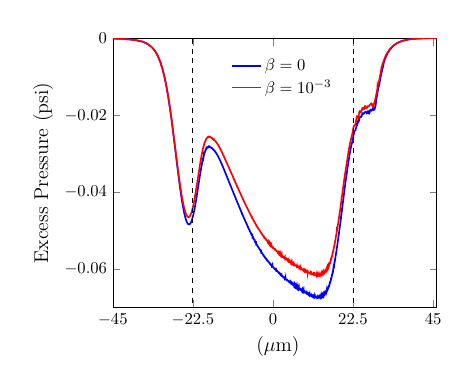
\begin{tikzpicture}[scale=0.6]

  \begin{axis}[
    scaled y ticks=false,
    xmin = -45,
    xmax = 46,
    ymin = -0.07,
    ymax = 0,
    xtick = {-45,-22.5,0,22.5,45},
    ylabel near ticks,
    xlabel = {\large $\xx$ ($\mu$m)},
    ylabel = {\large Excess Pressure (psi)},
    ytick = {-0.06,-0.04,-0.02,0},
    yticklabels = {$-0.06$,$-0.04$,$-0.02$,$0$},
    legend entries = {$\beta=0$,$\beta = 10^{-3}$},
    legend cell align=left,
    legend style={draw=none},
    legend style={at={(0.35,0.95)},anchor=north west}
  ]


\addplot[blue,line width=1pt] coordinates{
(-4.5000e+01,0.0000e+00)
(-4.4997e+01,-8.7460e-08)
(-4.4992e+01,-2.5521e-07)
(-4.4985e+01,-4.7224e-07)
(-4.4976e+01,-7.9185e-07)
(-4.4963e+01,-1.2411e-06)
(-4.4944e+01,-1.8827e-06)
(-4.4916e+01,-2.7939e-06)
(-4.4878e+01,-4.0902e-06)
(-4.4823e+01,-5.9326e-06)
(-4.4744e+01,-8.5518e-06)
(-4.4633e+01,-1.2276e-05)
(-4.4474e+01,-1.7578e-05)
(-4.4248e+01,-2.5154e-05)
(-4.3927e+01,-3.6076e-05)
(-4.3468e+01,-5.2171e-05)
(-4.2813e+01,-7.7039e-05)
(-4.1876e+01,-1.1925e-04)
(-4.0526e+01,-2.0308e-04)
(-3.8553e+01,-4.0943e-04)
(-3.6658e+01,-8.0040e-04)
(-3.5392e+01,-1.3060e-03)
(-3.4782e+01,-1.7054e-03)
(-3.4277e+01,-2.0557e-03)
(-3.3851e+01,-2.4522e-03)
(-3.3477e+01,-2.8474e-03)
(-3.3146e+01,-3.2684e-03)
(-3.2842e+01,-3.7048e-03)
(-3.2572e+01,-4.1560e-03)
(-3.2307e+01,-4.6371e-03)
(-3.2093e+01,-5.1006e-03)
(-3.1884e+01,-5.5610e-03)
(-3.1643e+01,-6.1393e-03)
(-3.1477e+01,-6.6381e-03)
(-3.1317e+01,-7.0839e-03)
(-3.1083e+01,-7.7654e-03)
(-3.0959e+01,-8.2844e-03)
(-3.0840e+01,-8.6678e-03)
(-3.0667e+01,-9.2827e-03)
(-3.0443e+01,-1.0132e-02)
(-3.0339e+01,-1.0696e-02)
(-3.0240e+01,-1.1099e-02)
(-3.0095e+01,-1.1734e-02)
(-2.9918e+01,-1.2554e-02)
(-2.9832e+01,-1.3100e-02)
(-2.9749e+01,-1.3497e-02)
(-2.9630e+01,-1.4104e-02)
(-2.9456e+01,-1.4998e-02)
(-2.9358e+01,-1.5680e-02)
(-2.9262e+01,-1.6198e-02)
(-2.9141e+01,-1.6916e-02)
(-2.9053e+01,-1.7512e-02)
(-2.8968e+01,-1.8040e-02)
(-2.8846e+01,-1.8775e-02)
(-2.8765e+01,-1.9388e-02)
(-2.8688e+01,-1.9885e-02)
(-2.8576e+01,-2.0599e-02)
(-2.8488e+01,-2.1260e-02)
(-2.8403e+01,-2.1839e-02)
(-2.8301e+01,-2.2536e-02)
(-2.8233e+01,-2.3088e-02)
(-2.8168e+01,-2.3558e-02)
(-2.8075e+01,-2.4197e-02)
(-2.7972e+01,-2.4949e-02)
(-2.7907e+01,-2.5489e-02)
(-2.7845e+01,-2.5952e-02)
(-2.7757e+01,-2.6574e-02)
(-2.7664e+01,-2.7277e-02)
(-2.7599e+01,-2.7804e-02)
(-2.7538e+01,-2.8277e-02)
(-2.7450e+01,-2.8897e-02)
(-2.7381e+01,-2.9468e-02)
(-2.7316e+01,-2.9958e-02)
(-2.7232e+01,-3.0566e-02)
(-2.7175e+01,-3.1053e-02)
(-2.7121e+01,-3.1470e-02)
(-2.7044e+01,-3.2017e-02)
(-2.6963e+01,-3.2624e-02)
(-2.6905e+01,-3.3090e-02)
(-2.6850e+01,-3.3517e-02)
(-2.6771e+01,-3.4058e-02)
(-2.6712e+01,-3.4543e-02)
(-2.6655e+01,-3.4957e-02)
(-2.6577e+01,-3.5491e-02)
(-2.6524e+01,-3.5926e-02)
(-2.6474e+01,-3.6293e-02)
(-2.6402e+01,-3.6767e-02)
(-2.6330e+01,-3.7274e-02)
(-2.6275e+01,-3.7679e-02)
(-2.6221e+01,-3.8063e-02)
(-2.6151e+01,-3.8504e-02)
(-2.6097e+01,-3.8904e-02)
(-2.6044e+01,-3.9259e-02)
(-2.5973e+01,-3.9690e-02)
(-2.5922e+01,-4.0056e-02)
(-2.5874e+01,-4.0375e-02)
(-2.5805e+01,-4.0768e-02)
(-2.5747e+01,-4.1146e-02)
(-2.5691e+01,-4.1479e-02)
(-2.5628e+01,-4.1838e-02)
(-2.5580e+01,-4.2144e-02)
(-2.5534e+01,-4.2430e-02)
(-2.5469e+01,-4.2758e-02)
(-2.5413e+01,-4.3080e-02)
(-2.5359e+01,-4.3364e-02)
(-2.5298e+01,-4.3666e-02)
(-2.5251e+01,-4.3926e-02)
(-2.5207e+01,-4.4174e-02)
(-2.5143e+01,-4.4445e-02)
(-2.5091e+01,-4.4708e-02)
(-2.5040e+01,-4.4941e-02)
(-2.4980e+01,-4.5189e-02)
(-2.4935e+01,-4.5402e-02)
(-2.4892e+01,-4.5607e-02)
(-2.4831e+01,-4.5819e-02)
(-2.4778e+01,-4.6031e-02)
(-2.4727e+01,-4.6219e-02)
(-2.4671e+01,-4.6405e-02)
(-2.4627e+01,-4.6571e-02)
(-2.4585e+01,-4.6739e-02)
(-2.4525e+01,-4.6895e-02)
(-2.4477e+01,-4.7046e-02)
(-2.4432e+01,-4.7188e-02)
(-2.4373e+01,-4.7320e-02)
(-2.4331e+01,-4.7439e-02)
(-2.4291e+01,-4.7566e-02)
(-2.4233e+01,-4.7665e-02)
(-2.4183e+01,-4.7767e-02)
(-2.4135e+01,-4.7857e-02)
(-2.4084e+01,-4.7936e-02)
(-2.4041e+01,-4.8012e-02)
(-2.4001e+01,-4.8098e-02)
(-2.3947e+01,-4.8146e-02)
(-2.3901e+01,-4.8195e-02)
(-2.3858e+01,-4.8251e-02)
(-2.3807e+01,-4.8278e-02)
(-2.3765e+01,-4.8305e-02)
(-2.3725e+01,-4.8352e-02)
(-2.3673e+01,-4.8351e-02)
(-2.3630e+01,-4.8353e-02)
(-2.3589e+01,-4.8375e-02)
(-2.3539e+01,-4.8355e-02)
(-2.3498e+01,-4.8338e-02)
(-2.3459e+01,-4.8345e-02)
(-2.3410e+01,-4.8304e-02)
(-2.3368e+01,-4.8265e-02)
(-2.3329e+01,-4.8248e-02)
(-2.3283e+01,-4.8193e-02)
(-2.3241e+01,-4.8137e-02)
(-2.3202e+01,-4.8100e-02)
(-2.3158e+01,-4.8032e-02)
(-2.3116e+01,-4.7956e-02)
(-2.3077e+01,-4.7897e-02)
(-2.3035e+01,-4.7817e-02)
(-2.2993e+01,-4.7728e-02)
(-2.2954e+01,-4.7649e-02)
(-2.2913e+01,-4.7558e-02)
(-2.2870e+01,-4.7444e-02)
(-2.2834e+01,-4.7353e-02)
(-2.2800e+01,-4.7293e-02)
(-2.2755e+01,-4.7160e-02)
(-2.2712e+01,-4.7013e-02)
(-2.2675e+01,-4.6900e-02)
(-2.2639e+01,-4.6804e-02)
(-2.2598e+01,-4.6667e-02)
(-2.2556e+01,-4.6508e-02)
(-2.2519e+01,-4.6377e-02)
(-2.2484e+01,-4.6265e-02)
(-2.2443e+01,-4.6114e-02)
(-2.2401e+01,-4.5936e-02)
(-2.2365e+01,-4.5790e-02)
(-2.2331e+01,-4.5670e-02)
(-2.2290e+01,-4.5501e-02)
(-2.2249e+01,-4.5304e-02)
(-2.2213e+01,-4.5146e-02)
(-2.2179e+01,-4.5019e-02)
(-2.2139e+01,-4.4833e-02)
(-2.2097e+01,-4.4618e-02)
(-2.2062e+01,-4.4449e-02)
(-2.2029e+01,-4.4317e-02)
(-2.1989e+01,-4.4115e-02)
(-2.1947e+01,-4.3883e-02)
(-2.1913e+01,-4.3704e-02)
(-2.1881e+01,-4.3570e-02)
(-2.1839e+01,-4.3353e-02)
(-2.1797e+01,-4.3104e-02)
(-2.1764e+01,-4.2918e-02)
(-2.1732e+01,-4.2784e-02)
(-2.1691e+01,-4.2553e-02)
(-2.1648e+01,-4.2287e-02)
(-2.1615e+01,-4.2094e-02)
(-2.1585e+01,-4.1964e-02)
(-2.1542e+01,-4.1718e-02)
(-2.1499e+01,-4.1437e-02)
(-2.1467e+01,-4.1240e-02)
(-2.1437e+01,-4.1115e-02)
(-2.1394e+01,-4.0857e-02)
(-2.1349e+01,-4.0559e-02)
(-2.1318e+01,-4.0357e-02)
(-2.1289e+01,-4.0247e-02)
(-2.1248e+01,-3.9990e-02)
(-2.1195e+01,-3.9648e-02)
(-2.1168e+01,-3.9423e-02)
(-2.1143e+01,-3.9394e-02)
(-2.1107e+01,-3.9140e-02)
(-2.1056e+01,-3.8848e-02)
(-2.1004e+01,-3.8476e-02)
(-2.0977e+01,-3.8277e-02)
(-2.0952e+01,-3.8226e-02)
(-2.0915e+01,-3.7979e-02)
(-2.0863e+01,-3.7679e-02)
(-2.0813e+01,-3.7317e-02)
(-2.0785e+01,-3.7121e-02)
(-2.0758e+01,-3.7051e-02)
(-2.0720e+01,-3.6804e-02)
(-2.0666e+01,-3.6488e-02)
(-2.0623e+01,-3.6171e-02)
(-2.0589e+01,-3.5993e-02)
(-2.0557e+01,-3.5828e-02)
(-2.0514e+01,-3.5588e-02)
(-2.0468e+01,-3.5290e-02)
(-2.0435e+01,-3.5085e-02)
(-2.0403e+01,-3.4962e-02)
(-2.0358e+01,-3.4709e-02)
(-2.0308e+01,-3.4402e-02)
(-2.0277e+01,-3.4197e-02)
(-2.0247e+01,-3.4118e-02)
(-2.0205e+01,-3.3878e-02)
(-2.0145e+01,-3.3560e-02)
(-2.0112e+01,-3.3307e-02)
(-2.0081e+01,-3.3254e-02)
(-2.0037e+01,-3.3004e-02)
(-1.9974e+01,-3.2686e-02)
(-1.9945e+01,-3.2444e-02)
(-1.9918e+01,-3.2479e-02)
(-1.9879e+01,-3.2246e-02)
(-1.9824e+01,-3.2026e-02)
(-1.9760e+01,-3.1692e-02)
(-1.9732e+01,-3.1504e-02)
(-1.9704e+01,-3.1521e-02)
(-1.9665e+01,-3.1318e-02)
(-1.9610e+01,-3.1119e-02)
(-1.9531e+01,-3.0781e-02)
(-1.9504e+01,-3.0560e-02)
(-1.9479e+01,-3.0673e-02)
(-1.9444e+01,-3.0469e-02)
(-1.9393e+01,-3.0339e-02)
(-1.9321e+01,-3.0081e-02)
(-1.9261e+01,-2.9845e-02)
(-1.9227e+01,-2.9731e-02)
(-1.9195e+01,-2.9718e-02)
(-1.9149e+01,-2.9575e-02)
(-1.9084e+01,-2.9411e-02)
(-1.9026e+01,-2.9218e-02)
(-1.8987e+01,-2.9131e-02)
(-1.8950e+01,-2.9099e-02)
(-1.8897e+01,-2.8986e-02)
(-1.8822e+01,-2.8826e-02)
(-1.8787e+01,-2.8691e-02)
(-1.8753e+01,-2.8760e-02)
(-1.8704e+01,-2.8645e-02)
(-1.8636e+01,-2.8566e-02)
(-1.8567e+01,-2.8430e-02)
(-1.8528e+01,-2.8373e-02)
(-1.8491e+01,-2.8412e-02)
(-1.8439e+01,-2.8345e-02)
(-1.8364e+01,-2.8291e-02)
(-1.8300e+01,-2.8202e-02)
(-1.8256e+01,-2.8190e-02)
(-1.8214e+01,-2.8214e-02)
(-1.8154e+01,-2.8190e-02)
(-1.8069e+01,-2.8153e-02)
(-1.8028e+01,-2.8093e-02)
(-1.7990e+01,-2.8205e-02)
(-1.7935e+01,-2.8169e-02)
(-1.7858e+01,-2.8193e-02)
(-1.7779e+01,-2.8166e-02)
(-1.7736e+01,-2.8170e-02)
(-1.7695e+01,-2.8258e-02)
(-1.7638e+01,-2.8259e-02)
(-1.7555e+01,-2.8300e-02)
(-1.7481e+01,-2.8298e-02)
(-1.7434e+01,-2.8330e-02)
(-1.7390e+01,-2.8409e-02)
(-1.7327e+01,-2.8436e-02)
(-1.7237e+01,-2.8485e-02)
(-1.7185e+01,-2.8483e-02)
(-1.7136e+01,-2.8585e-02)
(-1.7069e+01,-2.8614e-02)
(-1.6993e+01,-2.8660e-02)
(-1.6945e+01,-2.8684e-02)
(-1.6899e+01,-2.8779e-02)
(-1.6834e+01,-2.8817e-02)
(-1.6741e+01,-2.8881e-02)
(-1.6696e+01,-2.8879e-02)
(-1.6654e+01,-2.9019e-02)
(-1.6593e+01,-2.9041e-02)
(-1.6508e+01,-2.9127e-02)
(-1.6450e+01,-2.9150e-02)
(-1.6396e+01,-2.9247e-02)
(-1.6337e+01,-2.9303e-02)
(-1.6271e+01,-2.9373e-02)
(-1.6220e+01,-2.9427e-02)
(-1.6172e+01,-2.9523e-02)
(-1.6106e+01,-2.9593e-02)
(-1.6038e+01,-2.9663e-02)
(-1.5989e+01,-2.9729e-02)
(-1.5942e+01,-2.9832e-02)
(-1.5876e+01,-2.9911e-02)
(-1.5808e+01,-2.9991e-02)
(-1.5761e+01,-3.0062e-02)
(-1.5716e+01,-3.0175e-02)
(-1.5653e+01,-3.0257e-02)
(-1.5577e+01,-3.0357e-02)
(-1.5536e+01,-3.0417e-02)
(-1.5496e+01,-3.0554e-02)
(-1.5440e+01,-3.0621e-02)
(-1.5361e+01,-3.0752e-02)
(-1.5302e+01,-3.0828e-02)
(-1.5252e+01,-3.0941e-02)
(-1.5205e+01,-3.1042e-02)
(-1.5145e+01,-3.1150e-02)
(-1.5084e+01,-3.1246e-02)
(-1.5036e+01,-3.1342e-02)
(-1.4990e+01,-3.1459e-02)
(-1.4930e+01,-3.1565e-02)
(-1.4869e+01,-3.1668e-02)
(-1.4822e+01,-3.1765e-02)
(-1.4778e+01,-3.1887e-02)
(-1.4717e+01,-3.1995e-02)
(-1.4656e+01,-3.2101e-02)
(-1.4610e+01,-3.2198e-02)
(-1.4567e+01,-3.2324e-02)
(-1.4507e+01,-3.2433e-02)
(-1.4446e+01,-3.2543e-02)
(-1.4401e+01,-3.2640e-02)
(-1.4359e+01,-3.2768e-02)
(-1.4299e+01,-3.2878e-02)
(-1.4237e+01,-3.2990e-02)
(-1.4194e+01,-3.3086e-02)
(-1.4153e+01,-3.3217e-02)
(-1.4094e+01,-3.3324e-02)
(-1.4028e+01,-3.3445e-02)
(-1.3989e+01,-3.3529e-02)
(-1.3951e+01,-3.3673e-02)
(-1.3898e+01,-3.3765e-02)
(-1.3822e+01,-3.3913e-02)
(-1.3779e+01,-3.3985e-02)
(-1.3739e+01,-3.4141e-02)
(-1.3682e+01,-3.4237e-02)
(-1.3620e+01,-3.4359e-02)
(-1.3580e+01,-3.4446e-02)
(-1.3542e+01,-3.4586e-02)
(-1.3487e+01,-3.4684e-02)
(-1.3410e+01,-3.4826e-02)
(-1.3377e+01,-3.4876e-02)
(-1.3345e+01,-3.5063e-02)
(-1.3300e+01,-3.5115e-02)
(-1.3236e+01,-3.5266e-02)
(-1.3154e+01,-3.5404e-02)
(-1.3123e+01,-3.5455e-02)
(-1.3093e+01,-3.5648e-02)
(-1.3050e+01,-3.5690e-02)
(-1.2990e+01,-3.5838e-02)
(-1.2904e+01,-3.5988e-02)
(-1.2870e+01,-3.6049e-02)
(-1.2838e+01,-3.6225e-02)
(-1.2792e+01,-3.6284e-02)
(-1.2727e+01,-3.6433e-02)
(-1.2660e+01,-3.6545e-02)
(-1.2627e+01,-3.6622e-02)
(-1.2595e+01,-3.6776e-02)
(-1.2549e+01,-3.6845e-02)
(-1.2485e+01,-3.6988e-02)
(-1.2419e+01,-3.7100e-02)
(-1.2385e+01,-3.7176e-02)
(-1.2354e+01,-3.7330e-02)
(-1.2309e+01,-3.7398e-02)
(-1.2245e+01,-3.7540e-02)
(-1.2180e+01,-3.7649e-02)
(-1.2147e+01,-3.7726e-02)
(-1.2115e+01,-3.7877e-02)
(-1.2070e+01,-3.7947e-02)
(-1.2006e+01,-3.8088e-02)
(-1.1947e+01,-3.8189e-02)
(-1.1912e+01,-3.8275e-02)
(-1.1879e+01,-3.8414e-02)
(-1.1832e+01,-3.8495e-02)
(-1.1765e+01,-3.8633e-02)
(-1.1722e+01,-3.8705e-02)
(-1.1682e+01,-3.8840e-02)
(-1.1634e+01,-3.8933e-02)
(-1.1584e+01,-3.9036e-02)
(-1.1543e+01,-3.9125e-02)
(-1.1505e+01,-3.9243e-02)
(-1.1455e+01,-3.9344e-02)
(-1.1404e+01,-3.9439e-02)
(-1.1365e+01,-3.9529e-02)
(-1.1327e+01,-3.9647e-02)
(-1.1277e+01,-3.9746e-02)
(-1.1226e+01,-3.9840e-02)
(-1.1187e+01,-3.9927e-02)
(-1.1151e+01,-4.0047e-02)
(-1.1100e+01,-4.0144e-02)
(-1.1049e+01,-4.0238e-02)
(-1.1011e+01,-4.0322e-02)
(-1.0976e+01,-4.0445e-02)
(-1.0926e+01,-4.0539e-02)
(-1.0872e+01,-4.0635e-02)
(-1.0837e+01,-4.0713e-02)
(-1.0803e+01,-4.0843e-02)
(-1.0755e+01,-4.0929e-02)
(-1.0691e+01,-4.1044e-02)
(-1.0661e+01,-4.1092e-02)
(-1.0633e+01,-4.1258e-02)
(-1.0592e+01,-4.1307e-02)
(-1.0535e+01,-4.1439e-02)
(-1.0467e+01,-4.1545e-02)
(-1.0437e+01,-4.1591e-02)
(-1.0408e+01,-4.1773e-02)
(-1.0367e+01,-4.1819e-02)
(-1.0309e+01,-4.1952e-02)
(-1.0254e+01,-4.2034e-02)
(-1.0222e+01,-4.2113e-02)
(-1.0191e+01,-4.2251e-02)
(-1.0148e+01,-4.2321e-02)
(-1.0087e+01,-4.2444e-02)
(-1.0043e+01,-4.2509e-02)
(-1.0004e+01,-4.2621e-02)
(-9.9669e+00,-4.2714e-02)
(-9.9223e+00,-4.2815e-02)
(-9.8750e+00,-4.2896e-02)
(-9.8378e+00,-4.2980e-02)
(-9.8025e+00,-4.3092e-02)
(-9.7559e+00,-4.3182e-02)
(-9.7074e+00,-4.3265e-02)
(-9.6718e+00,-4.3343e-02)
(-9.6380e+00,-4.3461e-02)
(-9.5901e+00,-4.3547e-02)
(-9.5402e+00,-4.3631e-02)
(-9.5062e+00,-4.3704e-02)
(-9.4740e+00,-4.3828e-02)
(-9.4282e+00,-4.3908e-02)
(-9.3695e+00,-4.4007e-02)
(-9.3403e+00,-4.4052e-02)
(-9.3127e+00,-4.4210e-02)
(-9.2733e+00,-4.4257e-02)
(-9.2174e+00,-4.4380e-02)
(-9.1603e+00,-4.4463e-02)
(-9.1316e+00,-4.4521e-02)
(-9.1044e+00,-4.4671e-02)
(-9.0657e+00,-4.4720e-02)
(-9.0108e+00,-4.4841e-02)
(-8.9516e+00,-4.4929e-02)
(-8.9241e+00,-4.4977e-02)
(-8.8980e+00,-4.5137e-02)
(-8.8608e+00,-4.5176e-02)
(-8.8081e+00,-4.5297e-02)
(-8.7393e+00,-4.5402e-02)
(-8.7142e+00,-4.5418e-02)
(-8.6903e+00,-4.5618e-02)
(-8.6564e+00,-4.5629e-02)
(-8.6082e+00,-4.5751e-02)
(-8.5398e+00,-4.5862e-02)
(-8.5058e+00,-4.5917e-02)
(-8.4735e+00,-4.6052e-02)
(-8.4276e+00,-4.6120e-02)
(-8.3806e+00,-4.6202e-02)
(-8.3477e+00,-4.6266e-02)
(-8.3164e+00,-4.6383e-02)
(-8.2720e+00,-4.6456e-02)
(-8.2199e+00,-4.6539e-02)
(-8.1903e+00,-4.6586e-02)
(-8.1622e+00,-4.6723e-02)
(-8.1223e+00,-4.6775e-02)
(-8.0655e+00,-4.6882e-02)
(-8.0269e+00,-4.6926e-02)
(-7.9902e+00,-4.7035e-02)
(-7.9528e+00,-4.7105e-02)
(-7.9120e+00,-4.7190e-02)
(-7.8739e+00,-4.7257e-02)
(-7.8378e+00,-4.7344e-02)
(-7.7988e+00,-4.7424e-02)
(-7.7555e+00,-4.7496e-02)
(-7.7226e+00,-4.7562e-02)
(-7.6914e+00,-4.7670e-02)
(-7.6473e+00,-4.7743e-02)
(-7.6000e+00,-4.7812e-02)
(-7.5692e+00,-4.7870e-02)
(-7.5400e+00,-4.7993e-02)
(-7.4985e+00,-4.8055e-02)
(-7.4396e+00,-4.8146e-02)
(-7.4126e+00,-4.8166e-02)
(-7.3870e+00,-4.8338e-02)
(-7.3506e+00,-4.8366e-02)
(-7.2989e+00,-4.8476e-02)
(-7.2445e+00,-4.8536e-02)
(-7.2182e+00,-4.8583e-02)
(-7.1933e+00,-4.8738e-02)
(-7.1578e+00,-4.8770e-02)
(-7.1074e+00,-4.8875e-02)
(-7.0457e+00,-4.8948e-02)
(-7.0213e+00,-4.8967e-02)
(-6.9981e+00,-4.9158e-02)
(-6.9652e+00,-4.9167e-02)
(-6.9184e+00,-4.9275e-02)
(-6.8521e+00,-4.9363e-02)
(-6.8237e+00,-4.9392e-02)
(-6.7967e+00,-4.9550e-02)
(-6.7585e+00,-4.9584e-02)
(-6.7041e+00,-4.9683e-02)
(-6.6656e+00,-4.9714e-02)
(-6.6313e+00,-4.9813e-02)
(-6.5987e+00,-4.9886e-02)
(-6.5589e+00,-4.9966e-02)
(-6.5159e+00,-5.0020e-02)
(-6.4839e+00,-5.0080e-02)
(-6.4534e+00,-5.0183e-02)
(-6.4113e+00,-5.0246e-02)
(-6.3657e+00,-5.0302e-02)
(-6.3360e+00,-5.0352e-02)
(-6.3078e+00,-5.0470e-02)
(-6.2677e+00,-5.0522e-02)
(-6.2108e+00,-5.0597e-02)
(-6.1849e+00,-5.0606e-02)
(-6.1602e+00,-5.0774e-02)
(-6.1252e+00,-5.0791e-02)
(-6.0755e+00,-5.0888e-02)
(-6.0219e+00,-5.0937e-02)
(-5.9970e+00,-5.0966e-02)
(-5.9734e+00,-5.1121e-02)
(-5.9399e+00,-5.1139e-02)
(-5.8922e+00,-5.1233e-02)
(-5.8245e+00,-5.1305e-02)
(-5.8040e+00,-5.1277e-02)
(-5.7841e+00,-5.1512e-02)
(-5.7557e+00,-5.1478e-02)
(-5.7155e+00,-5.1583e-02)
(-5.6583e+00,-5.1653e-02)
(-5.5992e+00,-5.1735e-02)
(-5.5764e+00,-5.1730e-02)
(-5.5547e+00,-5.1923e-02)
(-5.5239e+00,-5.1915e-02)
(-5.4801e+00,-5.2014e-02)
(-5.4180e+00,-5.2090e-02)
(-5.3870e+00,-5.2120e-02)
(-5.3575e+00,-5.2243e-02)
(-5.3164e+00,-5.2287e-02)
(-5.2727e+00,-5.2346e-02)
(-5.2436e+00,-5.2386e-02)
(-5.2159e+00,-5.2495e-02)
(-5.1766e+00,-5.2543e-02)
(-5.1208e+00,-5.2611e-02)
(-5.0973e+00,-5.2601e-02)
(-5.0751e+00,-5.2782e-02)
(-5.0435e+00,-5.2777e-02)
(-4.9987e+00,-5.2871e-02)
(-4.9349e+00,-5.2938e-02)
(-4.9111e+00,-5.2935e-02)
(-4.8885e+00,-5.3108e-02)
(-4.8564e+00,-5.3105e-02)
(-4.8108e+00,-5.3196e-02)
(-4.7460e+00,-5.3256e-02)
(-4.7249e+00,-5.3231e-02)
(-4.7048e+00,-5.3439e-02)
(-4.6763e+00,-5.3409e-02)
(-4.6357e+00,-5.3501e-02)
(-4.5782e+00,-5.3561e-02)
(-4.5359e+00,-5.3606e-02)
(-4.5066e+00,-5.3656e-02)
(-4.4788e+00,-5.3748e-02)
(-4.4393e+00,-5.3793e-02)
(-4.3922e+00,-5.3837e-02)
(-4.3662e+00,-5.3855e-02)
(-4.3415e+00,-5.3984e-02)
(-4.3063e+00,-5.4004e-02)
(-4.2564e+00,-5.4075e-02)
(-4.2202e+00,-5.4091e-02)
(-4.1858e+00,-5.4163e-02)
(-4.1526e+00,-5.4208e-02)
(-4.1192e+00,-5.4270e-02)
(-4.0834e+00,-5.4318e-02)
(-4.0484e+00,-5.4363e-02)
(-4.0153e+00,-5.4416e-02)
(-3.9813e+00,-5.4473e-02)
(-3.9451e+00,-5.4520e-02)
(-3.9118e+00,-5.4564e-02)
(-3.8802e+00,-5.4628e-02)
(-3.8449e+00,-5.4682e-02)
(-3.8062e+00,-5.4721e-02)
(-3.7755e+00,-5.4761e-02)
(-3.7463e+00,-5.4844e-02)
(-3.7086e+00,-5.4890e-02)
(-3.6663e+00,-5.4924e-02)
(-3.6383e+00,-5.4955e-02)
(-3.6118e+00,-5.5063e-02)
(-3.5741e+00,-5.5097e-02)
(-3.5206e+00,-5.5143e-02)
(-3.4975e+00,-5.5132e-02)
(-3.4756e+00,-5.5307e-02)
(-3.4445e+00,-5.5299e-02)
(-3.4003e+00,-5.5378e-02)
(-3.3375e+00,-5.5417e-02)
(-3.3161e+00,-5.5397e-02)
(-3.2959e+00,-5.5597e-02)
(-3.2670e+00,-5.5571e-02)
(-3.2261e+00,-5.5653e-02)
(-3.1679e+00,-5.5700e-02)
(-3.1328e+00,-5.5718e-02)
(-3.0996e+00,-5.5793e-02)
(-3.0665e+00,-5.5833e-02)
(-3.0324e+00,-5.5888e-02)
(-2.9967e+00,-5.5927e-02)
(-2.9650e+00,-5.5972e-02)
(-2.9350e+00,-5.6039e-02)
(-2.8991e+00,-5.6088e-02)
(-2.8594e+00,-5.6117e-02)
(-2.8304e+00,-5.6150e-02)
(-2.8029e+00,-5.6242e-02)
(-2.7644e+00,-5.6278e-02)
(-2.7205e+00,-5.6303e-02)
(-2.6946e+00,-5.6323e-02)
(-2.6700e+00,-5.6444e-02)
(-2.6350e+00,-5.6462e-02)
(-2.5854e+00,-5.6515e-02)
(-2.5542e+00,-5.6513e-02)
(-2.5246e+00,-5.6609e-02)
(-2.4889e+00,-5.6637e-02)
(-2.4493e+00,-5.6670e-02)
(-2.4208e+00,-5.6695e-02)
(-2.3937e+00,-5.6786e-02)
(-2.3555e+00,-5.6817e-02)
(-2.3116e+00,-5.6839e-02)
(-2.2861e+00,-5.6852e-02)
(-2.2620e+00,-5.6973e-02)
(-2.2277e+00,-5.6986e-02)
(-2.1789e+00,-5.7037e-02)
(-2.1464e+00,-5.7033e-02)
(-2.1156e+00,-5.7113e-02)
(-2.0818e+00,-5.7142e-02)
(-2.0433e+00,-5.7175e-02)
(-2.0154e+00,-5.7196e-02)
(-1.9890e+00,-5.7286e-02)
(-1.9514e+00,-5.7313e-02)
(-1.9056e+00,-5.7337e-02)
(-1.8813e+00,-5.7335e-02)
(-1.8582e+00,-5.7467e-02)
(-1.8254e+00,-5.7468e-02)
(-1.7788e+00,-5.7524e-02)
(-1.7390e+00,-5.7525e-02)
(-1.7113e+00,-5.7563e-02)
(-1.6850e+00,-5.7642e-02)
(-1.6476e+00,-5.7671e-02)
(-1.6022e+00,-5.7693e-02)
(-1.5779e+00,-5.7691e-02)
(-1.5549e+00,-5.7819e-02)
(-1.5221e+00,-5.7819e-02)
(-1.4756e+00,-5.7874e-02)
(-1.4370e+00,-5.7876e-02)
(-1.4088e+00,-5.7917e-02)
(-1.3819e+00,-5.7986e-02)
(-1.3448e+00,-5.8019e-02)
(-1.3020e+00,-5.8038e-02)
(-1.2768e+00,-5.8045e-02)
(-1.2529e+00,-5.8156e-02)
(-1.2189e+00,-5.8165e-02)
(-1.1706e+00,-5.8214e-02)
(-1.1403e+00,-5.8206e-02)
(-1.1115e+00,-5.8293e-02)
(-1.0768e+00,-5.8315e-02)
(-1.0380e+00,-5.8344e-02)
(-1.0103e+00,-5.8359e-02)
(-9.8402e-01,-5.8443e-02)
(-9.4670e-01,-5.8467e-02)
(-9.0324e-01,-5.8490e-02)
(-8.7864e-01,-5.8489e-02)
(-8.5531e-01,-5.8606e-02)
(-8.2214e-01,-5.8610e-02)
(-7.7502e-01,-5.8661e-02)
(-7.4174e-01,-5.8656e-02)
(-7.1017e-01,-5.8719e-02)
(-6.7852e-01,-5.8745e-02)
(-6.4537e-01,-5.8786e-02)
(-6.1083e-01,-5.8809e-02)
(-5.8166e-01,-5.8840e-02)
(-5.5397e-01,-5.8900e-02)
(-5.1868e-01,-5.8933e-02)
(-4.7858e-01,-5.8950e-02)
(-4.5227e-01,-5.8961e-02)
(-4.2731e-01,-5.9053e-02)
(-3.9184e-01,-5.9069e-02)
(-3.4146e-01,-5.9100e-02)
(-3.1946e-01,-5.9064e-02)
(-2.9859e-01,-5.9223e-02)
(-2.6892e-01,-5.9198e-02)
(-2.2676e-01,-5.9259e-02)
(-1.6691e-01,-5.9275e-02)
(-1.3824e-01,-5.9179e-02)
(-1.1854e-01,-5.9390e-02)
(-9.4361e-02,-5.9394e-02)
(-5.9996e-02,-5.9440e-02)
(-1.1180e-02,-5.9463e-02)
(2.1106e-02,-5.9462e-02)
(5.1739e-02,-5.9522e-02)
(8.3486e-02,-5.9545e-02)
(1.1776e-01,-5.9576e-02)
(1.4811e-01,-5.9595e-02)
(1.7691e-01,-5.9646e-02)
(2.1022e-01,-5.9676e-02)
(2.4730e-01,-5.9692e-02)
(2.7508e-01,-5.9706e-02)
(3.0143e-01,-5.9779e-02)
(3.3717e-01,-5.9799e-02)
(3.7855e-01,-5.9809e-02)
(4.0332e-01,-5.9809e-02)
(4.2682e-01,-5.9915e-02)
(4.6022e-01,-5.9918e-02)
(5.0768e-01,-5.9951e-02)
(5.3554e-01,-5.9929e-02)
(5.6198e-01,-6.0027e-02)
(5.9751e-01,-6.0033e-02)
(6.3834e-01,-6.0047e-02)
(6.6329e-01,-6.0045e-02)
(6.8695e-01,-6.0151e-02)
(7.2059e-01,-6.0153e-02)
(7.6838e-01,-6.0182e-02)
(7.9481e-01,-6.0156e-02)
(8.1989e-01,-6.0267e-02)
(8.5554e-01,-6.0267e-02)
(9.0129e-01,-6.0283e-02)
(9.2414e-01,-6.0258e-02)
(9.4583e-01,-6.0400e-02)
(9.7665e-01,-6.0383e-02)
(1.0204e+00,-6.0428e-02)
(1.0636e+00,-6.0414e-02)
(1.0877e+00,-6.0420e-02)
(1.1105e+00,-6.0533e-02)
(1.1430e+00,-6.0533e-02)
(1.1891e+00,-6.0566e-02)
(1.2209e+00,-6.0545e-02)
(1.2512e+00,-6.0607e-02)
(1.2825e+00,-6.0626e-02)
(1.3164e+00,-6.0653e-02)
(1.3465e+00,-6.0668e-02)
(1.3751e+00,-6.0719e-02)
(1.4079e+00,-6.0747e-02)
(1.4447e+00,-6.0758e-02)
(1.4722e+00,-6.0771e-02)
(1.4983e+00,-6.0847e-02)
(1.5337e+00,-6.0865e-02)
(1.5750e+00,-6.0869e-02)
(1.5994e+00,-6.0867e-02)
(1.6225e+00,-6.0982e-02)
(1.6554e+00,-6.0983e-02)
(1.7021e+00,-6.1013e-02)
(1.7313e+00,-6.0990e-02)
(1.7589e+00,-6.1077e-02)
(1.7926e+00,-6.1089e-02)
(1.8306e+00,-6.1102e-02)
(1.8571e+00,-6.1109e-02)
(1.8821e+00,-6.1199e-02)
(1.9178e+00,-6.1212e-02)
(1.9623e+00,-6.1217e-02)
(1.9852e+00,-6.1202e-02)
(2.0070e+00,-6.1341e-02)
(2.0380e+00,-6.1329e-02)
(2.0819e+00,-6.1371e-02)
(2.1226e+00,-6.1353e-02)
(2.1475e+00,-6.1370e-02)
(2.1712e+00,-6.1470e-02)
(2.2047e+00,-6.1478e-02)
(2.2524e+00,-6.1498e-02)
(2.2775e+00,-6.1471e-02)
(2.3014e+00,-6.1595e-02)
(2.3352e+00,-6.1591e-02)
(2.3833e+00,-6.1614e-02)
(2.4071e+00,-6.1580e-02)
(2.4296e+00,-6.1721e-02)
(2.4616e+00,-6.1707e-02)
(2.5071e+00,-6.1744e-02)
(2.5393e+00,-6.1719e-02)
(2.5699e+00,-6.1774e-02)
(2.6002e+00,-6.1793e-02)
(2.6316e+00,-6.1827e-02)
(2.6646e+00,-6.1842e-02)
(2.6937e+00,-6.1865e-02)
(2.7214e+00,-6.1916e-02)
(2.7543e+00,-6.1943e-02)
(2.7914e+00,-6.1947e-02)
(2.8178e+00,-6.1956e-02)
(2.8429e+00,-6.2039e-02)
(2.8784e+00,-6.2051e-02)
(2.9205e+00,-6.2050e-02)
(2.9437e+00,-6.2041e-02)
(2.9657e+00,-6.2166e-02)
(2.9970e+00,-6.2157e-02)
(3.0415e+00,-6.2190e-02)
(3.0759e+00,-6.2166e-02)
(3.1039e+00,-6.2207e-02)
(3.1305e+00,-6.2254e-02)
(3.1641e+00,-6.2281e-02)
(3.2025e+00,-6.2278e-02)
(3.2276e+00,-6.2282e-02)
(3.2515e+00,-6.2375e-02)
(3.2854e+00,-6.2380e-02)
(3.3335e+00,-6.2387e-02)
(3.3548e+00,-6.2347e-02)
(3.3750e+00,-6.2507e-02)
(3.4037e+00,-6.2475e-02)
(3.4445e+00,-6.2520e-02)
(3.5025e+00,-6.2506e-02)
(3.5293e+00,-6.2376e-02)
(3.5489e+00,-6.2620e-02)
(3.5716e+00,-6.2609e-02)
(3.6040e+00,-6.2653e-02)
(3.6499e+00,-6.2656e-02)
(3.6827e+00,-6.2642e-02)
(3.7115e+00,-6.2681e-02)
(3.7388e+00,-6.2714e-02)
(3.7711e+00,-6.2742e-02)
(3.8073e+00,-6.2740e-02)
(3.8335e+00,-6.2746e-02)
(3.8584e+00,-6.2818e-02)
(3.8931e+00,-6.2827e-02)
(3.9339e+00,-6.2824e-02)
(3.9571e+00,-6.2810e-02)
(3.9790e+00,-6.2924e-02)
(4.0102e+00,-6.2913e-02)
(4.0546e+00,-6.2940e-02)
(4.0860e+00,-6.2913e-02)
(4.1159e+00,-6.2961e-02)
(4.1455e+00,-6.2973e-02)
(4.1761e+00,-6.3001e-02)
(4.2085e+00,-6.3010e-02)
(4.2370e+00,-6.3025e-02)
(4.2640e+00,-6.3068e-02)
(4.2962e+00,-6.3089e-02)
(4.3326e+00,-6.3089e-02)
(4.3584e+00,-6.3090e-02)
(4.3829e+00,-6.3165e-02)
(4.4177e+00,-6.3172e-02)
(4.4591e+00,-6.3170e-02)
(4.4818e+00,-6.3151e-02)
(4.5033e+00,-6.3269e-02)
(4.5339e+00,-6.3254e-02)
(4.5774e+00,-6.3285e-02)
(4.6115e+00,-6.3261e-02)
(4.6388e+00,-6.3294e-02)
(4.6647e+00,-6.3337e-02)
(4.6979e+00,-6.3359e-02)
(4.7360e+00,-6.3355e-02)
(4.7605e+00,-6.3350e-02)
(4.7837e+00,-6.3439e-02)
(4.8167e+00,-6.3439e-02)
(4.8635e+00,-6.3453e-02)
(4.8856e+00,-6.3410e-02)
(4.9066e+00,-6.3548e-02)
(4.9365e+00,-6.3522e-02)
(4.9789e+00,-6.3562e-02)
(5.0179e+00,-6.3541e-02)
(5.0421e+00,-6.3549e-02)
(5.0650e+00,-6.3635e-02)
(5.0975e+00,-6.3636e-02)
(5.1437e+00,-6.3653e-02)
(5.1672e+00,-6.3614e-02)
(5.1895e+00,-6.3735e-02)
(5.2212e+00,-6.3719e-02)
(5.2662e+00,-6.3749e-02)
(5.2932e+00,-6.3716e-02)
(5.3188e+00,-6.3804e-02)
(5.3522e+00,-6.3803e-02)
(5.3903e+00,-6.3812e-02)
(5.4145e+00,-6.3801e-02)
(5.4375e+00,-6.3894e-02)
(5.4701e+00,-6.3892e-02)
(5.5165e+00,-6.3909e-02)
(5.5391e+00,-6.3867e-02)
(5.5605e+00,-6.3998e-02)
(5.5910e+00,-6.3975e-02)
(5.6342e+00,-6.4012e-02)
(5.6675e+00,-6.3987e-02)
(5.6950e+00,-6.4024e-02)
(5.7211e+00,-6.4061e-02)
(5.7536e+00,-6.4086e-02)
(5.7906e+00,-6.4083e-02)
(5.8154e+00,-6.4082e-02)
(5.8389e+00,-6.4163e-02)
(5.8724e+00,-6.4167e-02)
(5.9199e+00,-6.4172e-02)
(5.9415e+00,-6.4107e-02)
(5.9610e+00,-6.4284e-02)
(5.9888e+00,-6.4243e-02)
(6.0284e+00,-6.4290e-02)
(6.0775e+00,-6.4273e-02)
(6.0996e+00,-6.4215e-02)
(6.1192e+00,-6.4391e-02)
(6.1470e+00,-6.4355e-02)
(6.1865e+00,-6.4399e-02)
(6.2326e+00,-6.4379e-02)
(6.2535e+00,-6.4342e-02)
(6.2732e+00,-6.4497e-02)
(6.3013e+00,-6.4463e-02)
(6.3412e+00,-6.4505e-02)
(6.3906e+00,-6.4488e-02)
(6.4128e+00,-6.4426e-02)
(6.4324e+00,-6.4606e-02)
(6.4602e+00,-6.4569e-02)
(6.4997e+00,-6.4611e-02)
(6.5439e+00,-6.4586e-02)
(6.5644e+00,-6.4561e-02)
(6.5840e+00,-6.4703e-02)
(6.6118e+00,-6.4672e-02)
(6.6513e+00,-6.4712e-02)
(6.7040e+00,-6.4697e-02)
(6.7279e+00,-6.4606e-02)
(6.7474e+00,-6.4810e-02)
(6.7748e+00,-6.4776e-02)
(6.8138e+00,-6.4815e-02)
(6.8507e+00,-6.4786e-02)
(6.8752e+00,-6.4798e-02)
(6.8985e+00,-6.4872e-02)
(6.9315e+00,-6.4876e-02)
(6.9784e+00,-6.4872e-02)
(6.9997e+00,-6.4807e-02)
(7.0192e+00,-6.4986e-02)
(7.0470e+00,-6.4943e-02)
(7.0865e+00,-6.4985e-02)
(7.1327e+00,-6.4956e-02)
(7.1524e+00,-6.4920e-02)
(7.1719e+00,-6.5080e-02)
(7.1997e+00,-6.5039e-02)
(7.2392e+00,-6.5079e-02)
(7.2911e+00,-6.5054e-02)
(7.3145e+00,-6.4965e-02)
(7.3341e+00,-6.5168e-02)
(7.3618e+00,-6.5131e-02)
(7.4013e+00,-6.5166e-02)
(7.4363e+00,-6.5132e-02)
(7.4617e+00,-6.5152e-02)
(7.4859e+00,-6.5211e-02)
(7.5194e+00,-6.5220e-02)
(7.5584e+00,-6.5206e-02)
(7.5810e+00,-6.5191e-02)
(7.6025e+00,-6.5299e-02)
(7.6331e+00,-6.5286e-02)
(7.6765e+00,-6.5302e-02)
(7.7049e+00,-6.5264e-02)
(7.7320e+00,-6.5329e-02)
(7.7624e+00,-6.5331e-02)
(7.7962e+00,-6.5336e-02)
(7.8223e+00,-6.5333e-02)
(7.8471e+00,-6.5396e-02)
(7.8797e+00,-6.5402e-02)
(7.9177e+00,-6.5391e-02)
(7.9409e+00,-6.5378e-02)
(7.9630e+00,-6.5478e-02)
(7.9943e+00,-6.5468e-02)
(8.0389e+00,-6.5476e-02)
(8.0633e+00,-6.5434e-02)
(8.0865e+00,-6.5541e-02)
(8.1194e+00,-6.5527e-02)
(8.1636e+00,-6.5524e-02)
(8.1844e+00,-6.5476e-02)
(8.2042e+00,-6.5629e-02)
(8.2323e+00,-6.5593e-02)
(8.2723e+00,-6.5626e-02)
(8.3201e+00,-6.5592e-02)
(8.3416e+00,-6.5533e-02)
(8.3611e+00,-6.5715e-02)
(8.3889e+00,-6.5676e-02)
(8.4283e+00,-6.5711e-02)
(8.4721e+00,-6.5672e-02)
(8.4923e+00,-6.5647e-02)
(8.5118e+00,-6.5797e-02)
(8.5396e+00,-6.5763e-02)
(8.5790e+00,-6.5796e-02)
(8.6304e+00,-6.5766e-02)
(8.6536e+00,-6.5674e-02)
(8.6731e+00,-6.5883e-02)
(8.7008e+00,-6.5846e-02)
(8.7403e+00,-6.5879e-02)
(8.7753e+00,-6.5840e-02)
(8.8005e+00,-6.5860e-02)
(8.8244e+00,-6.5924e-02)
(8.8579e+00,-6.5932e-02)
(8.8973e+00,-6.5916e-02)
(8.9196e+00,-6.5899e-02)
(8.9408e+00,-6.6015e-02)
(8.9709e+00,-6.6000e-02)
(9.0137e+00,-6.6018e-02)
(9.0442e+00,-6.5980e-02)
(9.0731e+00,-6.6023e-02)
(9.1015e+00,-6.6031e-02)
(9.1308e+00,-6.6058e-02)
(9.1619e+00,-6.6063e-02)
(9.1901e+00,-6.6073e-02)
(9.2168e+00,-6.6109e-02)
(9.2472e+00,-6.6128e-02)
(9.2831e+00,-6.6121e-02)
(9.3065e+00,-6.6116e-02)
(9.3287e+00,-6.6211e-02)
(9.3603e+00,-6.6207e-02)
(9.4052e+00,-6.6210e-02)
(9.4282e+00,-6.6166e-02)
(9.4499e+00,-6.6292e-02)
(9.4809e+00,-6.6272e-02)
(9.5249e+00,-6.6286e-02)
(9.5505e+00,-6.6243e-02)
(9.5749e+00,-6.6340e-02)
(9.6077e+00,-6.6331e-02)
(9.6462e+00,-6.6324e-02)
(9.6688e+00,-6.6306e-02)
(9.6903e+00,-6.6419e-02)
(9.7208e+00,-6.6406e-02)
(9.7642e+00,-6.6419e-02)
(9.7915e+00,-6.6380e-02)
(9.8174e+00,-6.6456e-02)
(9.8484e+00,-6.6455e-02)
(9.8835e+00,-6.6454e-02)
(9.9082e+00,-6.6447e-02)
(9.9316e+00,-6.6528e-02)
(9.9649e+00,-6.6527e-02)
(1.0006e+01,-6.6513e-02)
(1.0027e+01,-6.6485e-02)
(1.0048e+01,-6.6617e-02)
(1.0076e+01,-6.6593e-02)
(1.0118e+01,-6.6617e-02)
(1.0154e+01,-6.6579e-02)
(1.0178e+01,-6.6591e-02)
(1.0201e+01,-6.6670e-02)
(1.0233e+01,-6.6670e-02)
(1.0279e+01,-6.6657e-02)
(1.0300e+01,-6.6594e-02)
(1.0320e+01,-6.6766e-02)
(1.0347e+01,-6.6728e-02)
(1.0387e+01,-6.6759e-02)
(1.0427e+01,-6.6719e-02)
(1.0449e+01,-6.6708e-02)
(1.0470e+01,-6.6825e-02)
(1.0499e+01,-6.6806e-02)
(1.0541e+01,-6.6823e-02)
(1.0573e+01,-6.6784e-02)
(1.0599e+01,-6.6812e-02)
(1.0624e+01,-6.6855e-02)
(1.0656e+01,-6.6869e-02)
(1.0693e+01,-6.6849e-02)
(1.0716e+01,-6.6838e-02)
(1.0738e+01,-6.6933e-02)
(1.0769e+01,-6.6923e-02)
(1.0813e+01,-6.6920e-02)
(1.0835e+01,-6.6872e-02)
(1.0857e+01,-6.6999e-02)
(1.0887e+01,-6.6972e-02)
(1.0929e+01,-6.6985e-02)
(1.0957e+01,-6.6940e-02)
(1.0983e+01,-6.7009e-02)
(1.1013e+01,-6.7005e-02)
(1.1047e+01,-6.7002e-02)
(1.1072e+01,-6.6992e-02)
(1.1095e+01,-6.7062e-02)
(1.1128e+01,-6.7059e-02)
(1.1167e+01,-6.7039e-02)
(1.1188e+01,-6.7012e-02)
(1.1209e+01,-6.7129e-02)
(1.1238e+01,-6.7104e-02)
(1.1279e+01,-6.7117e-02)
(1.1311e+01,-6.7073e-02)
(1.1337e+01,-6.7101e-02)
(1.1362e+01,-6.7131e-02)
(1.1393e+01,-6.7144e-02)
(1.1429e+01,-6.7122e-02)
(1.1452e+01,-6.7110e-02)
(1.1475e+01,-6.7192e-02)
(1.1506e+01,-6.7181e-02)
(1.1551e+01,-6.7164e-02)
(1.1573e+01,-6.7093e-02)
(1.1592e+01,-6.7254e-02)
(1.1620e+01,-6.7211e-02)
(1.1659e+01,-6.7232e-02)
(1.1696e+01,-6.7184e-02)
(1.1719e+01,-6.7181e-02)
(1.1741e+01,-6.7261e-02)
(1.1772e+01,-6.7249e-02)
(1.1816e+01,-6.7236e-02)
(1.1837e+01,-6.7181e-02)
(1.1858e+01,-6.7306e-02)
(1.1887e+01,-6.7270e-02)
(1.1929e+01,-6.7280e-02)
(1.1959e+01,-6.7229e-02)
(1.1987e+01,-6.7256e-02)
(1.2014e+01,-6.7252e-02)
(1.2042e+01,-6.7274e-02)
(1.2071e+01,-6.7273e-02)
(1.2102e+01,-6.7263e-02)
(1.2129e+01,-6.7261e-02)
(1.2154e+01,-6.7288e-02)
(1.2184e+01,-6.7292e-02)
(1.2218e+01,-6.7270e-02)
(1.2243e+01,-6.7254e-02)
(1.2266e+01,-6.7318e-02)
(1.2298e+01,-6.7305e-02)
(1.2337e+01,-6.7275e-02)
(1.2359e+01,-6.7236e-02)
(1.2379e+01,-6.7350e-02)
(1.2407e+01,-6.7314e-02)
(1.2448e+01,-6.7319e-02)
(1.2481e+01,-6.7266e-02)
(1.2506e+01,-6.7274e-02)
(1.2529e+01,-6.7317e-02)
(1.2561e+01,-6.7310e-02)
(1.2600e+01,-6.7275e-02)
(1.2621e+01,-6.7239e-02)
(1.2642e+01,-6.7343e-02)
(1.2671e+01,-6.7308e-02)
(1.2712e+01,-6.7307e-02)
(1.2743e+01,-6.7252e-02)
(1.2769e+01,-6.7275e-02)
(1.2795e+01,-6.7282e-02)
(1.2825e+01,-6.7288e-02)
(1.2859e+01,-6.7256e-02)
(1.2883e+01,-6.7237e-02)
(1.2906e+01,-6.7293e-02)
(1.2939e+01,-6.7275e-02)
(1.2978e+01,-6.7239e-02)
(1.2999e+01,-6.7195e-02)
(1.3019e+01,-6.7302e-02)
(1.3048e+01,-6.7261e-02)
(1.3089e+01,-6.7258e-02)
(1.3121e+01,-6.7200e-02)
(1.3147e+01,-6.7208e-02)
(1.3171e+01,-6.7234e-02)
(1.3202e+01,-6.7226e-02)
(1.3239e+01,-6.7186e-02)
(1.3262e+01,-6.7152e-02)
(1.3283e+01,-6.7233e-02)
(1.3313e+01,-6.7200e-02)
(1.3357e+01,-6.7178e-02)
(1.3380e+01,-6.7113e-02)
(1.3403e+01,-6.7201e-02)
(1.3434e+01,-6.7159e-02)
(1.3480e+01,-6.7125e-02)
(1.3500e+01,-6.7031e-02)
(1.3520e+01,-6.7188e-02)
(1.3548e+01,-6.7121e-02)
(1.3587e+01,-6.7125e-02)
(1.3623e+01,-6.7056e-02)
(1.3646e+01,-6.7039e-02)
(1.3668e+01,-6.7097e-02)
(1.3700e+01,-6.7067e-02)
(1.3744e+01,-6.7026e-02)
(1.3765e+01,-6.6951e-02)
(1.3784e+01,-6.7074e-02)
(1.3812e+01,-6.7011e-02)
(1.3851e+01,-6.7006e-02)
(1.3893e+01,-6.6934e-02)
(1.3914e+01,-6.6888e-02)
(1.3934e+01,-6.6987e-02)
(1.3962e+01,-6.6934e-02)
(1.4002e+01,-6.6917e-02)
(1.4038e+01,-6.6845e-02)
(1.4062e+01,-6.6826e-02)
(1.4084e+01,-6.6869e-02)
(1.4116e+01,-6.6834e-02)
(1.4159e+01,-6.6776e-02)
(1.4180e+01,-6.6699e-02)
(1.4199e+01,-6.6821e-02)
(1.4227e+01,-6.6749e-02)
(1.4266e+01,-6.6735e-02)
(1.4311e+01,-6.6646e-02)
(1.4331e+01,-6.6571e-02)
(1.4350e+01,-6.6704e-02)
(1.4378e+01,-6.6625e-02)
(1.4417e+01,-6.6608e-02)
(1.4458e+01,-6.6519e-02)
(1.4479e+01,-6.6466e-02)
(1.4500e+01,-6.6551e-02)
(1.4529e+01,-6.6488e-02)
(1.4570e+01,-6.6450e-02)
(1.4603e+01,-6.6364e-02)
(1.4628e+01,-6.6342e-02)
(1.4652e+01,-6.6355e-02)
(1.4685e+01,-6.6312e-02)
(1.4723e+01,-6.6235e-02)
(1.4745e+01,-6.6174e-02)
(1.4766e+01,-6.6243e-02)
(1.4796e+01,-6.6175e-02)
(1.4839e+01,-6.6119e-02)
(1.4867e+01,-6.6028e-02)
(1.4893e+01,-6.6040e-02)
(1.4923e+01,-6.5985e-02)
(1.4958e+01,-6.5923e-02)
(1.4982e+01,-6.5862e-02)
(1.5004e+01,-6.5897e-02)
(1.5037e+01,-6.5829e-02)
(1.5083e+01,-6.5732e-02)
(1.5104e+01,-6.5612e-02)
(1.5123e+01,-6.5743e-02)
(1.5151e+01,-6.5640e-02)
(1.5190e+01,-6.5593e-02)
(1.5231e+01,-6.5470e-02)
(1.5253e+01,-6.5398e-02)
(1.5273e+01,-6.5466e-02)
(1.5303e+01,-6.5378e-02)
(1.5344e+01,-6.5304e-02)
(1.5378e+01,-6.5187e-02)
(1.5404e+01,-6.5144e-02)
(1.5428e+01,-6.5131e-02)
(1.5461e+01,-6.5060e-02)
(1.5499e+01,-6.4947e-02)
(1.5522e+01,-6.4863e-02)
(1.5543e+01,-6.4910e-02)
(1.5574e+01,-6.4813e-02)
(1.5617e+01,-6.4713e-02)
(1.5645e+01,-6.4592e-02)
(1.5671e+01,-6.4586e-02)
(1.5702e+01,-6.4496e-02)
(1.5737e+01,-6.4397e-02)
(1.5762e+01,-6.4309e-02)
(1.5786e+01,-6.4307e-02)
(1.5819e+01,-6.4207e-02)
(1.5860e+01,-6.4072e-02)
(1.5882e+01,-6.3967e-02)
(1.5903e+01,-6.4017e-02)
(1.5933e+01,-6.3899e-02)
(1.5975e+01,-6.3784e-02)
(1.6009e+01,-6.3634e-02)
(1.6035e+01,-6.3569e-02)
(1.6061e+01,-6.3518e-02)
(1.6093e+01,-6.3422e-02)
(1.6131e+01,-6.3274e-02)
(1.6155e+01,-6.3169e-02)
(1.6178e+01,-6.3179e-02)
(1.6210e+01,-6.3054e-02)
(1.6255e+01,-6.2891e-02)
(1.6279e+01,-6.2748e-02)
(1.6301e+01,-6.2778e-02)
(1.6333e+01,-6.2634e-02)
(1.6378e+01,-6.2472e-02)
(1.6404e+01,-6.2315e-02)
(1.6429e+01,-6.2308e-02)
(1.6463e+01,-6.2157e-02)
(1.6504e+01,-6.1980e-02)
(1.6527e+01,-6.1847e-02)
(1.6549e+01,-6.1870e-02)
(1.6579e+01,-6.1717e-02)
(1.6623e+01,-6.1547e-02)
(1.6656e+01,-6.1357e-02)
(1.6685e+01,-6.1262e-02)
(1.6711e+01,-6.1166e-02)
(1.6744e+01,-6.1036e-02)
(1.6782e+01,-6.0843e-02)
(1.6807e+01,-6.0707e-02)
(1.6831e+01,-6.0673e-02)
(1.6865e+01,-6.0506e-02)
(1.6914e+01,-6.0264e-02)
(1.6935e+01,-6.0093e-02)
(1.6955e+01,-6.0153e-02)
(1.6983e+01,-5.9967e-02)
(1.7023e+01,-5.9802e-02)
(1.7080e+01,-5.9493e-02)
(1.7102e+01,-5.9307e-02)
(1.7123e+01,-5.9344e-02)
(1.7154e+01,-5.9145e-02)
(1.7197e+01,-5.8946e-02)
(1.7248e+01,-5.8628e-02)
(1.7268e+01,-5.8457e-02)
(1.7287e+01,-5.8521e-02)
(1.7315e+01,-5.8316e-02)
(1.7354e+01,-5.8137e-02)
(1.7409e+01,-5.7812e-02)
(1.7441e+01,-5.7580e-02)
(1.7472e+01,-5.7451e-02)
(1.7504e+01,-5.7264e-02)
(1.7538e+01,-5.7073e-02)
(1.7570e+01,-5.6874e-02)
(1.7601e+01,-5.6715e-02)
(1.7634e+01,-5.6529e-02)
(1.7671e+01,-5.6300e-02)
(1.7701e+01,-5.6106e-02)
(1.7729e+01,-5.5979e-02)
(1.7764e+01,-5.5765e-02)
(1.7807e+01,-5.5483e-02)
(1.7834e+01,-5.5286e-02)
(1.7859e+01,-5.5218e-02)
(1.7895e+01,-5.4979e-02)
(1.7946e+01,-5.4655e-02)
(1.7973e+01,-5.4420e-02)
(1.7999e+01,-5.4354e-02)
(1.8036e+01,-5.4095e-02)
(1.8089e+01,-5.3751e-02)
(1.8114e+01,-5.3516e-02)
(1.8139e+01,-5.3472e-02)
(1.8174e+01,-5.3212e-02)
(1.8224e+01,-5.2895e-02)
(1.8264e+01,-5.2575e-02)
(1.8295e+01,-5.2382e-02)
(1.8324e+01,-5.2223e-02)
(1.8362e+01,-5.1969e-02)
(1.8411e+01,-5.1615e-02)
(1.8438e+01,-5.1391e-02)
(1.8463e+01,-5.1317e-02)
(1.8500e+01,-5.1044e-02)
(1.8552e+01,-5.0691e-02)
(1.8591e+01,-5.0367e-02)
(1.8624e+01,-5.0154e-02)
(1.8656e+01,-4.9945e-02)
(1.8695e+01,-4.9688e-02)
(1.8741e+01,-4.9337e-02)
(1.8772e+01,-4.9098e-02)
(1.8800e+01,-4.8966e-02)
(1.8841e+01,-4.8665e-02)
(1.8899e+01,-4.8234e-02)
(1.8926e+01,-4.7980e-02)
(1.8951e+01,-4.7925e-02)
(1.8987e+01,-4.7629e-02)
(1.9038e+01,-4.7278e-02)
(1.9110e+01,-4.6712e-02)
(1.9132e+01,-4.6458e-02)
(1.9153e+01,-4.6500e-02)
(1.9183e+01,-4.6208e-02)
(1.9225e+01,-4.5936e-02)
(1.9285e+01,-4.5473e-02)
(1.9371e+01,-4.4833e-02)
(1.9395e+01,-4.4544e-02)
(1.9418e+01,-4.4566e-02)
(1.9451e+01,-4.4249e-02)
(1.9497e+01,-4.3940e-02)
(1.9563e+01,-4.3425e-02)
(1.9626e+01,-4.2925e-02)
(1.9656e+01,-4.2658e-02)
(1.9683e+01,-4.2569e-02)
(1.9723e+01,-4.2241e-02)
(1.9779e+01,-4.1841e-02)
(1.9849e+01,-4.1273e-02)
(1.9876e+01,-4.1013e-02)
(1.9901e+01,-4.0970e-02)
(1.9936e+01,-4.0656e-02)
(1.9987e+01,-4.0310e-02)
(2.0059e+01,-3.9770e-02)
(2.0117e+01,-3.9311e-02)
(2.0152e+01,-3.9043e-02)
(2.0184e+01,-3.8877e-02)
(2.0231e+01,-3.8533e-02)
(2.0297e+01,-3.8068e-02)
(2.0340e+01,-3.7718e-02)
(2.0381e+01,-3.7475e-02)
(2.0429e+01,-3.7143e-02)
(2.0487e+01,-3.6741e-02)
(2.0527e+01,-3.6448e-02)
(2.0564e+01,-3.6259e-02)
(2.0616e+01,-3.5906e-02)
(2.0691e+01,-3.5416e-02)
(2.0725e+01,-3.5142e-02)
(2.0756e+01,-3.5043e-02)
(2.0801e+01,-3.4725e-02)
(2.0865e+01,-3.4347e-02)
(2.0955e+01,-3.3778e-02)
(2.0994e+01,-3.3480e-02)
(2.1032e+01,-3.3338e-02)
(2.1084e+01,-3.2991e-02)
(2.1159e+01,-3.2551e-02)
(2.1221e+01,-3.2133e-02)
(2.1268e+01,-3.1851e-02)
(2.1312e+01,-3.1608e-02)
(2.1371e+01,-3.1254e-02)
(2.1455e+01,-3.0741e-02)
(2.1493e+01,-3.0459e-02)
(2.1528e+01,-3.0347e-02)
(2.1578e+01,-3.0025e-02)
(2.1649e+01,-2.9645e-02)
(2.1749e+01,-2.9099e-02)
(2.1812e+01,-2.8738e-02)
(2.1867e+01,-2.8494e-02)
(2.1920e+01,-2.8262e-02)
(2.1985e+01,-2.8005e-02)
(2.2071e+01,-2.7654e-02)
(2.2118e+01,-2.7450e-02)
(2.2162e+01,-2.7364e-02)
(2.2224e+01,-2.7125e-02)
(2.2313e+01,-2.6813e-02)
(2.2437e+01,-2.6281e-02)
(2.2474e+01,-2.5979e-02)
(2.2509e+01,-2.5969e-02)
(2.2558e+01,-2.5655e-02)
(2.2628e+01,-2.5328e-02)
(2.2727e+01,-2.4827e-02)
(2.2867e+01,-2.4306e-02)
(2.2932e+01,-2.4112e-02)
(2.2993e+01,-2.4068e-02)
(2.3077e+01,-2.3965e-02)
(2.3196e+01,-2.3813e-02)
(2.3250e+01,-2.3594e-02)
(2.3301e+01,-2.3521e-02)
(2.3372e+01,-2.3209e-02)
(2.3474e+01,-2.2763e-02)
(2.3585e+01,-2.2232e-02)
(2.3690e+01,-2.1915e-02)
(2.3838e+01,-2.1759e-02)
(2.3871e+01,-2.1656e-02)
(2.3903e+01,-2.1879e-02)
(2.3948e+01,-2.1758e-02)
(2.4012e+01,-2.1746e-02)
(2.4102e+01,-2.1566e-02)
(2.4192e+01,-2.1301e-02)
(2.4283e+01,-2.0962e-02)
(2.4373e+01,-2.0628e-02)
(2.4458e+01,-2.0395e-02)
(2.4541e+01,-2.0301e-02)
(2.4624e+01,-2.0311e-02)
(2.4707e+01,-2.0367e-02)
(2.4790e+01,-2.0389e-02)
(2.4873e+01,-2.0301e-02)
(2.4954e+01,-2.0085e-02)
(2.5032e+01,-1.9797e-02)
(2.5107e+01,-1.9548e-02)
(2.5180e+01,-1.9413e-02)
(2.5254e+01,-1.9407e-02)
(2.5330e+01,-1.9486e-02)
(2.5407e+01,-1.9573e-02)
(2.5483e+01,-1.9600e-02)
(2.5557e+01,-1.9539e-02)
(2.5627e+01,-1.9433e-02)
(2.5694e+01,-1.9338e-02)
(2.5763e+01,-1.9262e-02)
(2.5833e+01,-1.9191e-02)
(2.5905e+01,-1.9139e-02)
(2.5977e+01,-1.9120e-02)
(2.6049e+01,-1.9120e-02)
(2.6120e+01,-1.9126e-02)
(2.6187e+01,-1.9170e-02)
(2.6252e+01,-1.9275e-02)
(2.6318e+01,-1.9401e-02)
(2.6385e+01,-1.9471e-02)
(2.6455e+01,-1.9416e-02)
(2.6528e+01,-1.9242e-02)
(2.6601e+01,-1.9041e-02)
(2.6673e+01,-1.8910e-02)
(2.6743e+01,-1.8897e-02)
(2.6811e+01,-1.9021e-02)
(2.6880e+01,-1.9236e-02)
(2.6951e+01,-1.9443e-02)
(2.7027e+01,-1.9526e-02)
(2.7108e+01,-1.9414e-02)
(2.7196e+01,-1.9119e-02)
(2.7279e+01,-1.8790e-02)
(2.7357e+01,-1.8588e-02)
(2.7440e+01,-1.8547e-02)
(2.7524e+01,-1.8639e-02)
(2.7616e+01,-1.8764e-02)
(2.7719e+01,-1.8793e-02)
(2.7842e+01,-1.8616e-02)
(2.7984e+01,-1.8236e-02)
(2.8117e+01,-1.8105e-02)
(2.8226e+01,-1.8382e-02)
(2.8296e+01,-1.8532e-02)
(2.8362e+01,-1.8585e-02)
(2.8455e+01,-1.8541e-02)
(2.8586e+01,-1.8343e-02)
(2.8653e+01,-1.8100e-02)
(2.8716e+01,-1.7937e-02)
(2.8805e+01,-1.7582e-02)
(2.8931e+01,-1.6881e-02)
(2.8989e+01,-1.6255e-02)
(2.9044e+01,-1.5998e-02)
(2.9122e+01,-1.5523e-02)
(2.9233e+01,-1.4992e-02)
(2.9390e+01,-1.4152e-02)
(2.9611e+01,-1.2899e-02)
(2.9640e+01,-1.2371e-02)
(2.9666e+01,-1.2755e-02)
(2.9704e+01,-1.2494e-02)
(2.9758e+01,-1.2451e-02)
(2.9835e+01,-1.2148e-02)
(2.9944e+01,-1.1675e-02)
(3.0098e+01,-1.0889e-02)
(3.0316e+01,-9.8210e-03)
(3.0623e+01,-8.4690e-03)
(3.1050e+01,-6.8934e-03)
(3.1167e+01,-6.1341e-03)
(3.1278e+01,-5.9907e-03)
(3.1434e+01,-5.4897e-03)
(3.1653e+01,-4.9949e-03)
(3.1960e+01,-4.3243e-03)
(3.2387e+01,-3.5765e-03)
(3.2976e+01,-2.7550e-03)
(3.3777e+01,-1.9421e-03)
(3.4853e+01,-1.2069e-03)
(3.6285e+01,-6.1818e-04)
(3.8185e+01,-2.1089e-04)
(4.0730e+01,1.8941e-05)
(4.4200e+01,1.1704e-04)
(4.8544e+01,1.4509e-04)
};

\addplot[red,line width=1pt] coordinates{
(-4.5000e+01,0.0000e+00)
(-4.4997e+01,-8.7287e-08)
(-4.4992e+01,-2.5477e-07)
(-4.4985e+01,-4.7137e-07)
(-4.4976e+01,-7.9040e-07)
(-4.4963e+01,-1.2388e-06)
(-4.4944e+01,-1.8793e-06)
(-4.4916e+01,-2.7887e-06)
(-4.4878e+01,-4.0825e-06)
(-4.4823e+01,-5.9214e-06)
(-4.4744e+01,-8.5355e-06)
(-4.4633e+01,-1.2252e-05)
(-4.4474e+01,-1.7543e-05)
(-4.4248e+01,-2.5103e-05)
(-4.3926e+01,-3.6001e-05)
(-4.3468e+01,-5.2057e-05)
(-4.2813e+01,-7.6859e-05)
(-4.1875e+01,-1.1895e-04)
(-4.0526e+01,-2.0254e-04)
(-3.8552e+01,-4.0836e-04)
(-3.6662e+01,-7.9723e-04)
(-3.5438e+01,-1.2848e-03)
(-3.4850e+01,-1.6582e-03)
(-3.4329e+01,-2.0046e-03)
(-3.3946e+01,-2.3650e-03)
(-3.3569e+01,-2.7288e-03)
(-3.3250e+01,-3.1286e-03)
(-3.2936e+01,-3.5433e-03)
(-3.2690e+01,-3.9532e-03)
(-3.2450e+01,-4.3567e-03)
(-3.2186e+01,-4.8573e-03)
(-3.1996e+01,-5.3000e-03)
(-3.1811e+01,-5.7166e-03)
(-3.1559e+01,-6.3166e-03)
(-3.1436e+01,-6.7515e-03)
(-3.1317e+01,-7.0656e-03)
(-3.1144e+01,-7.5731e-03)
(-3.0891e+01,-8.3539e-03)
(-3.0771e+01,-8.9110e-03)
(-3.0655e+01,-9.2976e-03)
(-3.0487e+01,-9.9354e-03)
(-3.0358e+01,-1.0514e-02)
(-3.0234e+01,-1.1038e-02)
(-3.0098e+01,-1.1646e-02)
(-2.9992e+01,-1.2180e-02)
(-2.9889e+01,-1.2678e-02)
(-2.9756e+01,-1.3314e-02)
(-2.9665e+01,-1.3852e-02)
(-2.9577e+01,-1.4307e-02)
(-2.9450e+01,-1.4962e-02)
(-2.9356e+01,-1.5554e-02)
(-2.9264e+01,-1.6066e-02)
(-2.9149e+01,-1.6724e-02)
(-2.9075e+01,-1.7242e-02)
(-2.9003e+01,-1.7675e-02)
(-2.8900e+01,-1.8284e-02)
(-2.8789e+01,-1.8996e-02)
(-2.8719e+01,-1.9508e-02)
(-2.8653e+01,-1.9946e-02)
(-2.8557e+01,-2.0548e-02)
(-2.8455e+01,-2.1241e-02)
(-2.8388e+01,-2.1750e-02)
(-2.8324e+01,-2.2199e-02)
(-2.8232e+01,-2.2803e-02)
(-2.8150e+01,-2.3411e-02)
(-2.8072e+01,-2.3957e-02)
(-2.8003e+01,-2.4477e-02)
(-2.7937e+01,-2.4959e-02)
(-2.7856e+01,-2.5524e-02)
(-2.7791e+01,-2.6038e-02)
(-2.7728e+01,-2.6500e-02)
(-2.7646e+01,-2.7071e-02)
(-2.7586e+01,-2.7563e-02)
(-2.7528e+01,-2.7990e-02)
(-2.7445e+01,-2.8559e-02)
(-2.7385e+01,-2.9055e-02)
(-2.7327e+01,-2.9477e-02)
(-2.7246e+01,-3.0039e-02)
(-2.7191e+01,-3.0500e-02)
(-2.7138e+01,-3.0886e-02)
(-2.7064e+01,-3.1400e-02)
(-2.6995e+01,-3.1919e-02)
(-2.6932e+01,-3.2368e-02)
(-2.6873e+01,-3.2809e-02)
(-2.6810e+01,-3.3256e-02)
(-2.6750e+01,-3.3691e-02)
(-2.6693e+01,-3.4103e-02)
(-2.6629e+01,-3.4540e-02)
(-2.6572e+01,-3.4956e-02)
(-2.6517e+01,-3.5345e-02)
(-2.6452e+01,-3.5769e-02)
(-2.6397e+01,-3.6163e-02)
(-2.6344e+01,-3.6526e-02)
(-2.6279e+01,-3.6937e-02)
(-2.6226e+01,-3.7309e-02)
(-2.6175e+01,-3.7648e-02)
(-2.6108e+01,-3.8044e-02)
(-2.6058e+01,-3.8394e-02)
(-2.6009e+01,-3.8706e-02)
(-2.5941e+01,-3.9088e-02)
(-2.5892e+01,-3.9414e-02)
(-2.5846e+01,-3.9701e-02)
(-2.5780e+01,-4.0052e-02)
(-2.5727e+01,-4.0373e-02)
(-2.5677e+01,-4.0657e-02)
(-2.5614e+01,-4.0979e-02)
(-2.5568e+01,-4.1251e-02)
(-2.5524e+01,-4.1503e-02)
(-2.5461e+01,-4.1793e-02)
(-2.5408e+01,-4.2074e-02)
(-2.5357e+01,-4.2322e-02)
(-2.5300e+01,-4.2582e-02)
(-2.5254e+01,-4.2809e-02)
(-2.5211e+01,-4.3029e-02)
(-2.5150e+01,-4.3265e-02)
(-2.5102e+01,-4.3484e-02)
(-2.5057e+01,-4.3684e-02)
(-2.4997e+01,-4.3897e-02)
(-2.4953e+01,-4.4082e-02)
(-2.4911e+01,-4.4261e-02)
(-2.4851e+01,-4.4446e-02)
(-2.4804e+01,-4.4616e-02)
(-2.4760e+01,-4.4775e-02)
(-2.4703e+01,-4.4934e-02)
(-2.4660e+01,-4.5074e-02)
(-2.4619e+01,-4.5216e-02)
(-2.4561e+01,-4.5346e-02)
(-2.4517e+01,-4.5466e-02)
(-2.4475e+01,-4.5587e-02)
(-2.4419e+01,-4.5692e-02)
(-2.4377e+01,-4.5787e-02)
(-2.4336e+01,-4.5891e-02)
(-2.4282e+01,-4.5970e-02)
(-2.4239e+01,-4.6043e-02)
(-2.4198e+01,-4.6125e-02)
(-2.4147e+01,-4.6182e-02)
(-2.4104e+01,-4.6233e-02)
(-2.4063e+01,-4.6295e-02)
(-2.4015e+01,-4.6331e-02)
(-2.3972e+01,-4.6361e-02)
(-2.3931e+01,-4.6401e-02)
(-2.3886e+01,-4.6419e-02)
(-2.3843e+01,-4.6430e-02)
(-2.3802e+01,-4.6449e-02)
(-2.3759e+01,-4.6451e-02)
(-2.3716e+01,-4.6443e-02)
(-2.3676e+01,-4.6441e-02)
(-2.3634e+01,-4.6428e-02)
(-2.3590e+01,-4.6397e-02)
(-2.3553e+01,-4.6379e-02)
(-2.3518e+01,-4.6381e-02)
(-2.3472e+01,-4.6331e-02)
(-2.3428e+01,-4.6268e-02)
(-2.3390e+01,-4.6225e-02)
(-2.3354e+01,-4.6196e-02)
(-2.3311e+01,-4.6132e-02)
(-2.3269e+01,-4.6051e-02)
(-2.3231e+01,-4.5988e-02)
(-2.3195e+01,-4.5937e-02)
(-2.3154e+01,-4.5857e-02)
(-2.3112e+01,-4.5755e-02)
(-2.3075e+01,-4.5673e-02)
(-2.3040e+01,-4.5608e-02)
(-2.2999e+01,-4.5507e-02)
(-2.2958e+01,-4.5385e-02)
(-2.2922e+01,-4.5286e-02)
(-2.2888e+01,-4.5208e-02)
(-2.2847e+01,-4.5088e-02)
(-2.2806e+01,-4.4945e-02)
(-2.2771e+01,-4.4831e-02)
(-2.2737e+01,-4.4742e-02)
(-2.2697e+01,-4.4605e-02)
(-2.2656e+01,-4.4442e-02)
(-2.2621e+01,-4.4314e-02)
(-2.2588e+01,-4.4216e-02)
(-2.2548e+01,-4.4061e-02)
(-2.2507e+01,-4.3880e-02)
(-2.2474e+01,-4.3740e-02)
(-2.2441e+01,-4.3633e-02)
(-2.2401e+01,-4.3463e-02)
(-2.2360e+01,-4.3264e-02)
(-2.2327e+01,-4.3112e-02)
(-2.2295e+01,-4.3000e-02)
(-2.2255e+01,-4.2814e-02)
(-2.2214e+01,-4.2598e-02)
(-2.2182e+01,-4.2437e-02)
(-2.2151e+01,-4.2320e-02)
(-2.2110e+01,-4.2120e-02)
(-2.2069e+01,-4.1888e-02)
(-2.2037e+01,-4.1717e-02)
(-2.2007e+01,-4.1599e-02)
(-2.1966e+01,-4.1384e-02)
(-2.1925e+01,-4.1137e-02)
(-2.1893e+01,-4.0959e-02)
(-2.1864e+01,-4.0842e-02)
(-2.1822e+01,-4.0613e-02)
(-2.1780e+01,-4.0350e-02)
(-2.1750e+01,-4.0166e-02)
(-2.1721e+01,-4.0052e-02)
(-2.1679e+01,-3.9814e-02)
(-2.1635e+01,-3.9529e-02)
(-2.1606e+01,-3.9337e-02)
(-2.1579e+01,-3.9248e-02)
(-2.1540e+01,-3.9011e-02)
(-2.1485e+01,-3.8676e-02)
(-2.1457e+01,-3.8425e-02)
(-2.1431e+01,-3.8395e-02)
(-2.1394e+01,-3.8138e-02)
(-2.1341e+01,-3.7828e-02)
(-2.1311e+01,-3.7569e-02)
(-2.1283e+01,-3.7493e-02)
(-2.1242e+01,-3.7226e-02)
(-2.1193e+01,-3.6912e-02)
(-2.1166e+01,-3.6691e-02)
(-2.1141e+01,-3.6643e-02)
(-2.1105e+01,-3.6398e-02)
(-2.1054e+01,-3.6102e-02)
(-2.1010e+01,-3.5774e-02)
(-2.0981e+01,-3.5597e-02)
(-2.0953e+01,-3.5479e-02)
(-2.0913e+01,-3.5238e-02)
(-2.0856e+01,-3.4881e-02)
(-2.0829e+01,-3.4623e-02)
(-2.0804e+01,-3.4611e-02)
(-2.0767e+01,-3.4354e-02)
(-2.0715e+01,-3.4068e-02)
(-2.0673e+01,-3.3752e-02)
(-2.0641e+01,-3.3584e-02)
(-2.0611e+01,-3.3438e-02)
(-2.0568e+01,-3.3198e-02)
(-2.0521e+01,-3.2896e-02)
(-2.0491e+01,-3.2697e-02)
(-2.0462e+01,-3.2605e-02)
(-2.0421e+01,-3.2369e-02)
(-2.0363e+01,-3.2043e-02)
(-2.0333e+01,-3.1792e-02)
(-2.0305e+01,-3.1755e-02)
(-2.0264e+01,-3.1510e-02)
(-2.0207e+01,-3.1217e-02)
(-2.0174e+01,-3.0965e-02)
(-2.0143e+01,-3.0901e-02)
(-2.0098e+01,-3.0657e-02)
(-2.0045e+01,-3.0383e-02)
(-2.0015e+01,-3.0184e-02)
(-1.9986e+01,-3.0141e-02)
(-1.9946e+01,-2.9929e-02)
(-1.9888e+01,-2.9674e-02)
(-1.9846e+01,-2.9421e-02)
(-1.9806e+01,-2.9279e-02)
(-1.9766e+01,-2.9099e-02)
(-1.9724e+01,-2.8937e-02)
(-1.9680e+01,-2.8747e-02)
(-1.9640e+01,-2.8583e-02)
(-1.9603e+01,-2.8459e-02)
(-1.9558e+01,-2.8298e-02)
(-1.9508e+01,-2.8096e-02)
(-1.9471e+01,-2.7943e-02)
(-1.9436e+01,-2.7873e-02)
(-1.9386e+01,-2.7706e-02)
(-1.9327e+01,-2.7497e-02)
(-1.9293e+01,-2.7353e-02)
(-1.9261e+01,-2.7341e-02)
(-1.9215e+01,-2.7192e-02)
(-1.9150e+01,-2.7022e-02)
(-1.9103e+01,-2.6845e-02)
(-1.9059e+01,-2.6772e-02)
(-1.9013e+01,-2.6658e-02)
(-1.8964e+01,-2.6557e-02)
(-1.8916e+01,-2.6446e-02)
(-1.8870e+01,-2.6363e-02)
(-1.8823e+01,-2.6283e-02)
(-1.8772e+01,-2.6193e-02)
(-1.8723e+01,-2.6107e-02)
(-1.8676e+01,-2.6047e-02)
(-1.8627e+01,-2.5987e-02)
(-1.8571e+01,-2.5913e-02)
(-1.8523e+01,-2.5848e-02)
(-1.8477e+01,-2.5824e-02)
(-1.8424e+01,-2.5779e-02)
(-1.8358e+01,-2.5714e-02)
(-1.8317e+01,-2.5660e-02)
(-1.8277e+01,-2.5703e-02)
(-1.8221e+01,-2.5660e-02)
(-1.8142e+01,-2.5628e-02)
(-1.8094e+01,-2.5568e-02)
(-1.8050e+01,-2.5623e-02)
(-1.7988e+01,-2.5599e-02)
(-1.7913e+01,-2.5585e-02)
(-1.7871e+01,-2.5557e-02)
(-1.7830e+01,-2.5635e-02)
(-1.7772e+01,-2.5624e-02)
(-1.7690e+01,-2.5646e-02)
(-1.7632e+01,-2.5624e-02)
(-1.7577e+01,-2.5675e-02)
(-1.7520e+01,-2.5691e-02)
(-1.7457e+01,-2.5721e-02)
(-1.7401e+01,-2.5738e-02)
(-1.7348e+01,-2.5783e-02)
(-1.7288e+01,-2.5817e-02)
(-1.7217e+01,-2.5845e-02)
(-1.7168e+01,-2.5862e-02)
(-1.7123e+01,-2.5938e-02)
(-1.7058e+01,-2.5968e-02)
(-1.6965e+01,-2.6011e-02)
(-1.6926e+01,-2.5994e-02)
(-1.6888e+01,-2.6126e-02)
(-1.6834e+01,-2.6125e-02)
(-1.6758e+01,-2.6194e-02)
(-1.6650e+01,-2.6244e-02)
(-1.6614e+01,-2.6224e-02)
(-1.6580e+01,-2.6378e-02)
(-1.6531e+01,-2.6368e-02)
(-1.6461e+01,-2.6447e-02)
(-1.6362e+01,-2.6511e-02)
(-1.6305e+01,-2.6541e-02)
(-1.6250e+01,-2.6625e-02)
(-1.6192e+01,-2.6675e-02)
(-1.6129e+01,-2.6736e-02)
(-1.6079e+01,-2.6787e-02)
(-1.6031e+01,-2.6870e-02)
(-1.5968e+01,-2.6934e-02)
(-1.5900e+01,-2.6997e-02)
(-1.5853e+01,-2.7051e-02)
(-1.5809e+01,-2.7150e-02)
(-1.5747e+01,-2.7216e-02)
(-1.5668e+01,-2.7299e-02)
(-1.5628e+01,-2.7339e-02)
(-1.5590e+01,-2.7467e-02)
(-1.5536e+01,-2.7517e-02)
(-1.5458e+01,-2.7629e-02)
(-1.5394e+01,-2.7698e-02)
(-1.5347e+01,-2.7779e-02)
(-1.5303e+01,-2.7880e-02)
(-1.5241e+01,-2.7967e-02)
(-1.5173e+01,-2.8056e-02)
(-1.5131e+01,-2.8123e-02)
(-1.5091e+01,-2.8242e-02)
(-1.5033e+01,-2.8320e-02)
(-1.4952e+01,-2.8440e-02)
(-1.4912e+01,-2.8489e-02)
(-1.4874e+01,-2.8632e-02)
(-1.4819e+01,-2.8698e-02)
(-1.4742e+01,-2.8829e-02)
(-1.4694e+01,-2.8894e-02)
(-1.4648e+01,-2.9017e-02)
(-1.4592e+01,-2.9106e-02)
(-1.4533e+01,-2.9206e-02)
(-1.4488e+01,-2.9288e-02)
(-1.4445e+01,-2.9403e-02)
(-1.4387e+01,-2.9499e-02)
(-1.4323e+01,-2.9601e-02)
(-1.4283e+01,-2.9677e-02)
(-1.4244e+01,-2.9802e-02)
(-1.4189e+01,-2.9889e-02)
(-1.4110e+01,-3.0018e-02)
(-1.4074e+01,-3.0067e-02)
(-1.4040e+01,-3.0223e-02)
(-1.3992e+01,-3.0281e-02)
(-1.3924e+01,-3.0418e-02)
(-1.3852e+01,-3.0522e-02)
(-1.3818e+01,-3.0588e-02)
(-1.3785e+01,-3.0733e-02)
(-1.3739e+01,-3.0794e-02)
(-1.3672e+01,-3.0926e-02)
(-1.3594e+01,-3.1045e-02)
(-1.3562e+01,-3.1093e-02)
(-1.3531e+01,-3.1260e-02)
(-1.3488e+01,-3.1303e-02)
(-1.3427e+01,-3.1435e-02)
(-1.3340e+01,-3.1574e-02)
(-1.3306e+01,-3.1626e-02)
(-1.3274e+01,-3.1786e-02)
(-1.3229e+01,-3.1839e-02)
(-1.3164e+01,-3.1974e-02)
(-1.3089e+01,-3.2086e-02)
(-1.3057e+01,-3.2137e-02)
(-1.3027e+01,-3.2301e-02)
(-1.2984e+01,-3.2347e-02)
(-1.2923e+01,-3.2479e-02)
(-1.2837e+01,-3.2613e-02)
(-1.2808e+01,-3.2645e-02)
(-1.2781e+01,-3.2830e-02)
(-1.2742e+01,-3.2855e-02)
(-1.2687e+01,-3.2984e-02)
(-1.2609e+01,-3.3114e-02)
(-1.2558e+01,-3.3206e-02)
(-1.2516e+01,-3.3304e-02)
(-1.2476e+01,-3.3406e-02)
(-1.2426e+01,-3.3504e-02)
(-1.2371e+01,-3.3594e-02)
(-1.2333e+01,-3.3673e-02)
(-1.2296e+01,-3.3790e-02)
(-1.2244e+01,-3.3880e-02)
(-1.2184e+01,-3.3978e-02)
(-1.2150e+01,-3.4041e-02)
(-1.2117e+01,-3.4175e-02)
(-1.2070e+01,-3.4245e-02)
(-1.2004e+01,-3.4370e-02)
(-1.1962e+01,-3.4433e-02)
(-1.1921e+01,-3.4553e-02)
(-1.1875e+01,-3.4637e-02)
(-1.1824e+01,-3.4731e-02)
(-1.1785e+01,-3.4808e-02)
(-1.1748e+01,-3.4920e-02)
(-1.1698e+01,-3.5010e-02)
(-1.1644e+01,-3.5102e-02)
(-1.1608e+01,-3.5171e-02)
(-1.1575e+01,-3.5295e-02)
(-1.1527e+01,-3.5374e-02)
(-1.1459e+01,-3.5491e-02)
(-1.1428e+01,-3.5528e-02)
(-1.1399e+01,-3.5687e-02)
(-1.1358e+01,-3.5733e-02)
(-1.1300e+01,-3.5859e-02)
(-1.1232e+01,-3.5958e-02)
(-1.1203e+01,-3.5997e-02)
(-1.1177e+01,-3.6162e-02)
(-1.1138e+01,-3.6196e-02)
(-1.1084e+01,-3.6317e-02)
(-1.1007e+01,-3.6437e-02)
(-1.0978e+01,-3.6471e-02)
(-1.0950e+01,-3.6635e-02)
(-1.0911e+01,-3.6669e-02)
(-1.0856e+01,-3.6790e-02)
(-1.0778e+01,-3.6903e-02)
(-1.0753e+01,-3.6911e-02)
(-1.0730e+01,-3.7113e-02)
(-1.0698e+01,-3.7112e-02)
(-1.0651e+01,-3.7229e-02)
(-1.0585e+01,-3.7334e-02)
(-1.0518e+01,-3.7450e-02)
(-1.0490e+01,-3.7477e-02)
(-1.0465e+01,-3.7648e-02)
(-1.0428e+01,-3.7675e-02)
(-1.0375e+01,-3.7794e-02)
(-1.0301e+01,-3.7906e-02)
(-1.0273e+01,-3.7940e-02)
(-1.0246e+01,-3.8104e-02)
(-1.0208e+01,-3.8139e-02)
(-1.0153e+01,-3.8258e-02)
(-1.0082e+01,-3.8358e-02)
(-1.0057e+01,-3.8379e-02)
(-1.0034e+01,-3.8567e-02)
(-1.0000e+01,-3.8579e-02)
(-9.9525e+00,-3.8695e-02)
(-9.8849e+00,-3.8804e-02)
(-9.8380e+00,-3.8882e-02)
(-9.8030e+00,-3.8964e-02)
(-9.7697e+00,-3.9066e-02)
(-9.7242e+00,-3.9148e-02)
(-9.6737e+00,-3.9224e-02)
(-9.6419e+00,-3.9284e-02)
(-9.6118e+00,-3.9407e-02)
(-9.5689e+00,-3.9472e-02)
(-9.5080e+00,-3.9572e-02)
(-9.4775e+00,-3.9606e-02)
(-9.4486e+00,-3.9749e-02)
(-9.4076e+00,-3.9799e-02)
(-9.3492e+00,-3.9906e-02)
(-9.3127e+00,-3.9948e-02)
(-9.2780e+00,-4.0063e-02)
(-9.2361e+00,-4.0131e-02)
(-9.1900e+00,-4.0207e-02)
(-9.1565e+00,-4.0268e-02)
(-9.1248e+00,-4.0376e-02)
(-9.0802e+00,-4.0448e-02)
(-9.0294e+00,-4.0524e-02)
(-8.9996e+00,-4.0573e-02)
(-8.9714e+00,-4.0701e-02)
(-8.9312e+00,-4.0756e-02)
(-8.8741e+00,-4.0860e-02)
(-8.8381e+00,-4.0904e-02)
(-8.8039e+00,-4.1016e-02)
(-8.7631e+00,-4.1085e-02)
(-8.7182e+00,-4.1163e-02)
(-8.6853e+00,-4.1223e-02)
(-8.6540e+00,-4.1330e-02)
(-8.6106e+00,-4.1403e-02)
(-8.5609e+00,-4.1480e-02)
(-8.5317e+00,-4.1528e-02)
(-8.5039e+00,-4.1655e-02)
(-8.4644e+00,-4.1709e-02)
(-8.4083e+00,-4.1813e-02)
(-8.3737e+00,-4.1854e-02)
(-8.3409e+00,-4.1967e-02)
(-8.3003e+00,-4.2033e-02)
(-8.2550e+00,-4.2108e-02)
(-8.2236e+00,-4.2161e-02)
(-8.1938e+00,-4.2270e-02)
(-8.1515e+00,-4.2335e-02)
(-8.0993e+00,-4.2413e-02)
(-8.0720e+00,-4.2444e-02)
(-8.0461e+00,-4.2582e-02)
(-8.0093e+00,-4.2619e-02)
(-7.9569e+00,-4.2720e-02)
(-7.9125e+00,-4.2770e-02)
(-7.8813e+00,-4.2836e-02)
(-7.8517e+00,-4.2932e-02)
(-7.8096e+00,-4.2998e-02)
(-7.7601e+00,-4.3064e-02)
(-7.7325e+00,-4.3099e-02)
(-7.7064e+00,-4.3227e-02)
(-7.6691e+00,-4.3268e-02)
(-7.6162e+00,-4.3360e-02)
(-7.5784e+00,-4.3399e-02)
(-7.5425e+00,-4.3484e-02)
(-7.5074e+00,-4.3546e-02)
(-7.4715e+00,-4.3621e-02)
(-7.4334e+00,-4.3684e-02)
(-7.3982e+00,-4.3747e-02)
(-7.3648e+00,-4.3824e-02)
(-7.3279e+00,-4.3895e-02)
(-7.2853e+00,-4.3956e-02)
(-7.2553e+00,-4.4008e-02)
(-7.2267e+00,-4.4114e-02)
(-7.1862e+00,-4.4173e-02)
(-7.1343e+00,-4.4243e-02)
(-7.1084e+00,-4.4267e-02)
(-7.0838e+00,-4.4415e-02)
(-7.0488e+00,-4.4445e-02)
(-6.9991e+00,-4.4542e-02)
(-6.9508e+00,-4.4592e-02)
(-6.9234e+00,-4.4639e-02)
(-6.8974e+00,-4.4764e-02)
(-6.8605e+00,-4.4810e-02)
(-6.8080e+00,-4.4898e-02)
(-6.7740e+00,-4.4929e-02)
(-6.7417e+00,-4.5030e-02)
(-6.7048e+00,-4.5089e-02)
(-6.6637e+00,-4.5152e-02)
(-6.6327e+00,-4.5202e-02)
(-6.6033e+00,-4.5301e-02)
(-6.5638e+00,-4.5361e-02)
(-6.5175e+00,-4.5417e-02)
(-6.4903e+00,-4.5454e-02)
(-6.4644e+00,-4.5578e-02)
(-6.4276e+00,-4.5619e-02)
(-6.3754e+00,-4.5700e-02)
(-6.3432e+00,-4.5723e-02)
(-6.3127e+00,-4.5828e-02)
(-6.2750e+00,-4.5878e-02)
(-6.2322e+00,-4.5934e-02)
(-6.2033e+00,-4.5973e-02)
(-6.1759e+00,-4.6079e-02)
(-6.1368e+00,-4.6127e-02)
(-6.0850e+00,-4.6187e-02)
(-6.0604e+00,-4.6195e-02)
(-6.0371e+00,-4.6347e-02)
(-6.0040e+00,-4.6362e-02)
(-5.9569e+00,-4.6448e-02)
(-5.9010e+00,-4.6493e-02)
(-5.8789e+00,-4.6496e-02)
(-5.8580e+00,-4.6668e-02)
(-5.8283e+00,-4.6664e-02)
(-5.7860e+00,-4.6752e-02)
(-5.7260e+00,-4.6821e-02)
(-5.6937e+00,-4.6849e-02)
(-5.6632e+00,-4.6949e-02)
(-5.6269e+00,-4.6996e-02)
(-5.5865e+00,-4.7051e-02)
(-5.5571e+00,-4.7090e-02)
(-5.5292e+00,-4.7185e-02)
(-5.4903e+00,-4.7236e-02)
(-5.4450e+00,-4.7288e-02)
(-5.4191e+00,-4.7313e-02)
(-5.3944e+00,-4.7435e-02)
(-5.3594e+00,-4.7467e-02)
(-5.3097e+00,-4.7547e-02)
(-5.2758e+00,-4.7570e-02)
(-5.2437e+00,-4.7655e-02)
(-5.2098e+00,-4.7706e-02)
(-5.1725e+00,-4.7764e-02)
(-5.1414e+00,-4.7808e-02)
(-5.1119e+00,-4.7888e-02)
(-5.0757e+00,-4.7943e-02)
(-5.0345e+00,-4.7992e-02)
(-5.0065e+00,-4.8026e-02)
(-4.9800e+00,-4.8126e-02)
(-4.9424e+00,-4.8170e-02)
(-4.8926e+00,-4.8228e-02)
(-4.8687e+00,-4.8228e-02)
(-4.8460e+00,-4.8374e-02)
(-4.8138e+00,-4.8384e-02)
(-4.7681e+00,-4.8465e-02)
(-4.7164e+00,-4.8504e-02)
(-4.6945e+00,-4.8504e-02)
(-4.6738e+00,-4.8662e-02)
(-4.6443e+00,-4.8657e-02)
(-4.6023e+00,-4.8737e-02)
(-4.5428e+00,-4.8795e-02)
(-4.5173e+00,-4.8798e-02)
(-4.4931e+00,-4.8930e-02)
(-4.4587e+00,-4.8945e-02)
(-4.4098e+00,-4.9015e-02)
(-4.3787e+00,-4.9022e-02)
(-4.3492e+00,-4.9111e-02)
(-4.3144e+00,-4.9148e-02)
(-4.2756e+00,-4.9190e-02)
(-4.2473e+00,-4.9218e-02)
(-4.2205e+00,-4.9304e-02)
(-4.1834e+00,-4.9342e-02)
(-4.1394e+00,-4.9378e-02)
(-4.1146e+00,-4.9390e-02)
(-4.0910e+00,-4.9509e-02)
(-4.0575e+00,-4.9527e-02)
(-4.0099e+00,-4.9589e-02)
(-3.9766e+00,-4.9597e-02)
(-3.9450e+00,-4.9667e-02)
(-3.9130e+00,-4.9706e-02)
(-3.8791e+00,-4.9756e-02)
(-3.8464e+00,-4.9792e-02)
(-3.8154e+00,-4.9844e-02)
(-3.7830e+00,-4.9894e-02)
(-3.7477e+00,-4.9934e-02)
(-3.7170e+00,-4.9971e-02)
(-3.6878e+00,-5.0035e-02)
(-3.6539e+00,-5.0083e-02)
(-3.6152e+00,-5.0117e-02)
(-3.5875e+00,-5.0145e-02)
(-3.5611e+00,-5.0235e-02)
(-3.5245e+00,-5.0273e-02)
(-3.4800e+00,-5.0306e-02)
(-3.4558e+00,-5.0316e-02)
(-3.4328e+00,-5.0444e-02)
(-3.4002e+00,-5.0460e-02)
(-3.3538e+00,-5.0523e-02)
(-3.3170e+00,-5.0533e-02)
(-3.2883e+00,-5.0586e-02)
(-3.2610e+00,-5.0656e-02)
(-3.2255e+00,-5.0703e-02)
(-3.1835e+00,-5.0731e-02)
(-3.1582e+00,-5.0750e-02)
(-3.1342e+00,-5.0863e-02)
(-3.1001e+00,-5.0887e-02)
(-3.0516e+00,-5.0940e-02)
(-3.0240e+00,-5.0938e-02)
(-2.9978e+00,-5.1047e-02)
(-2.9611e+00,-5.1072e-02)
(-2.9174e+00,-5.1105e-02)
(-2.8934e+00,-5.1112e-02)
(-2.8705e+00,-5.1239e-02)
(-2.8380e+00,-5.1252e-02)
(-2.7919e+00,-5.1309e-02)
(-2.7561e+00,-5.1312e-02)
(-2.7272e+00,-5.1365e-02)
(-2.6998e+00,-5.1427e-02)
(-2.6650e+00,-5.1470e-02)
(-2.6246e+00,-5.1491e-02)
(-2.5989e+00,-5.1509e-02)
(-2.5746e+00,-5.1612e-02)
(-2.5401e+00,-5.1634e-02)
(-2.4910e+00,-5.1672e-02)
(-2.4671e+00,-5.1659e-02)
(-2.4445e+00,-5.1792e-02)
(-2.4123e+00,-5.1795e-02)
(-2.3666e+00,-5.1849e-02)
(-2.3310e+00,-5.1846e-02)
(-2.3025e+00,-5.1894e-02)
(-2.2755e+00,-5.1952e-02)
(-2.2410e+00,-5.1992e-02)
(-2.2009e+00,-5.2008e-02)
(-2.1756e+00,-5.2021e-02)
(-2.1517e+00,-5.2121e-02)
(-2.1176e+00,-5.2139e-02)
(-2.0692e+00,-5.2174e-02)
(-2.0452e+00,-5.2157e-02)
(-2.0225e+00,-5.2284e-02)
(-1.9901e+00,-5.2285e-02)
(-1.9442e+00,-5.2335e-02)
(-1.9122e+00,-5.2327e-02)
(-1.8818e+00,-5.2389e-02)
(-1.8511e+00,-5.2416e-02)
(-1.8186e+00,-5.2456e-02)
(-1.7870e+00,-5.2481e-02)
(-1.7570e+00,-5.2520e-02)
(-1.7261e+00,-5.2560e-02)
(-1.6927e+00,-5.2590e-02)
(-1.6625e+00,-5.2616e-02)
(-1.6339e+00,-5.2665e-02)
(-1.6019e+00,-5.2703e-02)
(-1.5645e+00,-5.2726e-02)
(-1.5387e+00,-5.2740e-02)
(-1.5143e+00,-5.2826e-02)
(-1.4795e+00,-5.2849e-02)
(-1.4301e+00,-5.2877e-02)
(-1.4102e+00,-5.2840e-02)
(-1.3904e+00,-5.3009e-02)
(-1.3622e+00,-5.2981e-02)
(-1.3222e+00,-5.3048e-02)
(-1.2654e+00,-5.3075e-02)
(-1.2435e+00,-5.3049e-02)
(-1.2227e+00,-5.3197e-02)
(-1.1932e+00,-5.3181e-02)
(-1.1512e+00,-5.3243e-02)
(-1.0984e+00,-5.3258e-02)
(-1.0746e+00,-5.3206e-02)
(-1.0548e+00,-5.3388e-02)
(-1.0267e+00,-5.3371e-02)
(-9.8668e-01,-5.3432e-02)
(-9.3760e-01,-5.3441e-02)
(-9.1743e-01,-5.3417e-02)
(-8.9764e-01,-5.3573e-02)
(-8.6951e-01,-5.3550e-02)
(-8.2953e-01,-5.3612e-02)
(-7.7275e-01,-5.3637e-02)
(-7.5236e-01,-5.3600e-02)
(-7.3258e-01,-5.3763e-02)
(-7.0446e-01,-5.3734e-02)
(-6.6450e-01,-5.3797e-02)
(-6.0775e-01,-5.3818e-02)
(-5.8759e-01,-5.3780e-02)
(-5.6781e-01,-5.3944e-02)
(-5.3971e-01,-5.3913e-02)
(-4.9977e-01,-5.3975e-02)
(-4.4304e-01,-5.3992e-02)
(-4.1324e-01,-5.3917e-02)
(-3.9347e-01,-5.4067e-02)
(-3.7190e-01,-5.4106e-02)
(-3.4124e-01,-5.4135e-02)
(-2.9767e-01,-5.4165e-02)
(-2.5725e-01,-5.4171e-02)
(-2.3339e-01,-5.4177e-02)
(-2.1076e-01,-5.4273e-02)
(-1.7859e-01,-5.4279e-02)
(-1.3288e-01,-5.4312e-02)
(-1.0679e-01,-5.4293e-02)
(-8.2051e-02,-5.4386e-02)
(-4.7411e-02,-5.4393e-02)
(-6.6175e-03,-5.4409e-02)
(1.6328e-02,-5.4398e-02)
(3.8097e-02,-5.4508e-02)
(6.9042e-02,-5.4505e-02)
(1.1301e-01,-5.4542e-02)
(1.4446e-01,-5.4527e-02)
(1.7429e-01,-5.4575e-02)
(2.0341e-01,-5.4594e-02)
(2.3323e-01,-5.4630e-02)
(2.6515e-01,-5.4649e-02)
(2.9470e-01,-5.4668e-02)
(3.2275e-01,-5.4704e-02)
(3.5330e-01,-5.4734e-02)
(3.8822e-01,-5.4747e-02)
(4.1436e-01,-5.4756e-02)
(4.3917e-01,-5.4825e-02)
(4.7273e-01,-5.4842e-02)
(5.1349e-01,-5.4848e-02)
(5.3626e-01,-5.4836e-02)
(5.5785e-01,-5.4949e-02)
(5.8856e-01,-5.4945e-02)
(6.3218e-01,-5.4979e-02)
(6.6377e-01,-5.4959e-02)
(6.9373e-01,-5.5003e-02)
(7.2234e-01,-5.5023e-02)
(7.5109e-01,-5.5062e-02)
(7.8255e-01,-5.5084e-02)
(8.1413e-01,-5.5099e-02)
(8.4409e-01,-5.5119e-02)
(8.7270e-01,-5.5151e-02)
(9.0142e-01,-5.5185e-02)
(9.3283e-01,-5.5210e-02)
(9.6449e-01,-5.5224e-02)
(9.9453e-01,-5.5244e-02)
(1.0230e+00,-5.5276e-02)
(1.0515e+00,-5.5312e-02)
(1.0828e+00,-5.5339e-02)
(1.1151e+00,-5.5352e-02)
(1.1431e+00,-5.5374e-02)
(1.1696e+00,-5.5423e-02)
(1.2013e+00,-5.5451e-02)
(1.2382e+00,-5.5459e-02)
(1.2631e+00,-5.5464e-02)
(1.2868e+00,-5.5551e-02)
(1.3205e+00,-5.5564e-02)
(1.3652e+00,-5.5572e-02)
(1.3866e+00,-5.5545e-02)
(1.4070e+00,-5.5690e-02)
(1.4359e+00,-5.5674e-02)
(1.4770e+00,-5.5719e-02)
(1.5218e+00,-5.5705e-02)
(1.5432e+00,-5.5692e-02)
(1.5635e+00,-5.5831e-02)
(1.5924e+00,-5.5818e-02)
(1.6334e+00,-5.5861e-02)
(1.6806e+00,-5.5846e-02)
(1.7019e+00,-5.5813e-02)
(1.7216e+00,-5.5982e-02)
(1.7496e+00,-5.5958e-02)
(1.7894e+00,-5.6006e-02)
(1.8389e+00,-5.5990e-02)
(1.8612e+00,-5.5940e-02)
(1.8809e+00,-5.6122e-02)
(1.9089e+00,-5.6098e-02)
(1.9487e+00,-5.6144e-02)
(1.9930e+00,-5.6122e-02)
(2.0135e+00,-5.6109e-02)
(2.0332e+00,-5.6254e-02)
(2.0612e+00,-5.6234e-02)
(2.1009e+00,-5.6278e-02)
(2.1544e+00,-5.6266e-02)
(2.1785e+00,-5.6178e-02)
(2.1982e+00,-5.6386e-02)
(2.2242e+00,-5.6366e-02)
(2.2613e+00,-5.6411e-02)
(2.3067e+00,-5.6390e-02)
(2.3271e+00,-5.6367e-02)
(2.3468e+00,-5.6517e-02)
(2.3748e+00,-5.6493e-02)
(2.4146e+00,-5.6535e-02)
(2.4655e+00,-5.6517e-02)
(2.4885e+00,-5.6447e-02)
(2.5081e+00,-5.6640e-02)
(2.5361e+00,-5.6613e-02)
(2.5759e+00,-5.6654e-02)
(2.6110e+00,-5.6627e-02)
(2.6362e+00,-5.6650e-02)
(2.6600e+00,-5.6716e-02)
(2.6934e+00,-5.6730e-02)
(2.7337e+00,-5.6724e-02)
(2.7556e+00,-5.6710e-02)
(2.7763e+00,-5.6828e-02)
(2.8058e+00,-5.6817e-02)
(2.8478e+00,-5.6846e-02)
(2.8815e+00,-5.6820e-02)
(2.9072e+00,-5.6848e-02)
(2.9316e+00,-5.6902e-02)
(2.9640e+00,-5.6920e-02)
(3.0028e+00,-5.6914e-02)
(3.0252e+00,-5.6903e-02)
(3.0465e+00,-5.7009e-02)
(3.0767e+00,-5.7002e-02)
(3.1197e+00,-5.7024e-02)
(3.1479e+00,-5.6995e-02)
(3.1747e+00,-5.7057e-02)
(3.2045e+00,-5.7066e-02)
(3.2394e+00,-5.7075e-02)
(3.2635e+00,-5.7071e-02)
(3.2863e+00,-5.7151e-02)
(3.3189e+00,-5.7155e-02)
(3.3650e+00,-5.7155e-02)
(3.3860e+00,-5.7093e-02)
(3.4057e+00,-5.7264e-02)
(3.4336e+00,-5.7229e-02)
(3.4734e+00,-5.7270e-02)
(3.5119e+00,-5.7244e-02)
(3.5346e+00,-5.7245e-02)
(3.5560e+00,-5.7337e-02)
(3.5866e+00,-5.7335e-02)
(3.6299e+00,-5.7354e-02)
(3.6555e+00,-5.7323e-02)
(3.6797e+00,-5.7407e-02)
(3.7120e+00,-5.7407e-02)
(3.7503e+00,-5.7412e-02)
(3.7726e+00,-5.7393e-02)
(3.7938e+00,-5.7497e-02)
(3.8240e+00,-5.7489e-02)
(3.8668e+00,-5.7515e-02)
(3.8941e+00,-5.7486e-02)
(3.9200e+00,-5.7554e-02)
(3.9504e+00,-5.7561e-02)
(3.9852e+00,-5.7572e-02)
(4.0097e+00,-5.7567e-02)
(4.0330e+00,-5.7640e-02)
(4.0658e+00,-5.7648e-02)
(4.1065e+00,-5.7651e-02)
(4.1278e+00,-5.7623e-02)
(4.1480e+00,-5.7743e-02)
(4.1767e+00,-5.7727e-02)
(4.2175e+00,-5.7763e-02)
(4.2535e+00,-5.7744e-02)
(4.2772e+00,-5.7755e-02)
(4.2997e+00,-5.7828e-02)
(4.3317e+00,-5.7836e-02)
(4.3772e+00,-5.7846e-02)
(4.3987e+00,-5.7790e-02)
(4.4184e+00,-5.7940e-02)
(4.4463e+00,-5.7913e-02)
(4.4860e+00,-5.7954e-02)
(4.5231e+00,-5.7935e-02)
(4.5462e+00,-5.7941e-02)
(4.5682e+00,-5.8021e-02)
(4.5994e+00,-5.8025e-02)
(4.6437e+00,-5.8041e-02)
(4.6654e+00,-5.8003e-02)
(4.6861e+00,-5.8120e-02)
(4.7154e+00,-5.8103e-02)
(4.7571e+00,-5.8137e-02)
(4.7884e+00,-5.8113e-02)
(4.8149e+00,-5.8149e-02)
(4.8400e+00,-5.8180e-02)
(4.8707e+00,-5.8205e-02)
(4.9064e+00,-5.8204e-02)
(4.9300e+00,-5.8198e-02)
(4.9524e+00,-5.8276e-02)
(4.9842e+00,-5.8279e-02)
(5.0295e+00,-5.8287e-02)
(5.0506e+00,-5.8227e-02)
(5.0703e+00,-5.8381e-02)
(5.0982e+00,-5.8349e-02)
(5.1378e+00,-5.8389e-02)
(5.1732e+00,-5.8365e-02)
(5.1968e+00,-5.8377e-02)
(5.2193e+00,-5.8443e-02)
(5.2512e+00,-5.8451e-02)
(5.2966e+00,-5.8452e-02)
(5.3171e+00,-5.8387e-02)
(5.3367e+00,-5.8553e-02)
(5.3646e+00,-5.8513e-02)
(5.4043e+00,-5.8554e-02)
(5.4387e+00,-5.8526e-02)
(5.4627e+00,-5.8543e-02)
(5.4854e+00,-5.8603e-02)
(5.5178e+00,-5.8612e-02)
(5.5579e+00,-5.8608e-02)
(5.5788e+00,-5.8578e-02)
(5.5986e+00,-5.8697e-02)
(5.6267e+00,-5.8676e-02)
(5.6667e+00,-5.8706e-02)
(5.7022e+00,-5.8682e-02)
(5.7254e+00,-5.8690e-02)
(5.7473e+00,-5.8761e-02)
(5.7786e+00,-5.8764e-02)
(5.8229e+00,-5.8766e-02)
(5.8443e+00,-5.8709e-02)
(5.8639e+00,-5.8854e-02)
(5.8918e+00,-5.8825e-02)
(5.9314e+00,-5.8857e-02)
(5.9641e+00,-5.8827e-02)
(5.9888e+00,-5.8849e-02)
(6.0122e+00,-5.8897e-02)
(6.0434e+00,-5.8910e-02)
(6.0816e+00,-5.8901e-02)
(6.1030e+00,-5.8879e-02)
(6.1233e+00,-5.8985e-02)
(6.1522e+00,-5.8970e-02)
(6.1932e+00,-5.8991e-02)
(6.2225e+00,-5.8959e-02)
(6.2502e+00,-5.8997e-02)
(6.2772e+00,-5.9005e-02)
(6.3048e+00,-5.9031e-02)
(6.3347e+00,-5.9038e-02)
(6.3627e+00,-5.9044e-02)
(6.3891e+00,-5.9068e-02)
(6.4172e+00,-5.9087e-02)
(6.4486e+00,-5.9092e-02)
(6.4747e+00,-5.9092e-02)
(6.4994e+00,-5.9137e-02)
(6.5290e+00,-5.9150e-02)
(6.5642e+00,-5.9146e-02)
(6.5873e+00,-5.9132e-02)
(6.6092e+00,-5.9215e-02)
(6.6403e+00,-5.9212e-02)
(6.6846e+00,-5.9211e-02)
(6.7057e+00,-5.9149e-02)
(6.7253e+00,-5.9301e-02)
(6.7532e+00,-5.9271e-02)
(6.7928e+00,-5.9300e-02)
(6.8252e+00,-5.9264e-02)
(6.8498e+00,-5.9288e-02)
(6.8733e+00,-5.9336e-02)
(6.9043e+00,-5.9351e-02)
(6.9426e+00,-5.9339e-02)
(6.9640e+00,-5.9316e-02)
(6.9842e+00,-5.9429e-02)
(7.0130e+00,-5.9414e-02)
(7.0539e+00,-5.9435e-02)
(7.0838e+00,-5.9401e-02)
(7.1102e+00,-5.9439e-02)
(7.1352e+00,-5.9464e-02)
(7.1648e+00,-5.9489e-02)
(7.1993e+00,-5.9481e-02)
(7.2228e+00,-5.9476e-02)
(7.2451e+00,-5.9555e-02)
(7.2768e+00,-5.9558e-02)
(7.3186e+00,-5.9552e-02)
(7.3389e+00,-5.9511e-02)
(7.3585e+00,-5.9652e-02)
(7.3863e+00,-5.9626e-02)
(7.4259e+00,-5.9658e-02)
(7.4627e+00,-5.9625e-02)
(7.4849e+00,-5.9627e-02)
(7.5061e+00,-5.9719e-02)
(7.5361e+00,-5.9718e-02)
(7.5787e+00,-5.9727e-02)
(7.6020e+00,-5.9690e-02)
(7.6240e+00,-5.9792e-02)
(7.6554e+00,-5.9784e-02)
(7.7000e+00,-5.9785e-02)
(7.7209e+00,-5.9720e-02)
(7.7405e+00,-5.9886e-02)
(7.7684e+00,-5.9854e-02)
(7.8080e+00,-5.9887e-02)
(7.8401e+00,-5.9850e-02)
(7.8649e+00,-5.9877e-02)
(7.8884e+00,-5.9926e-02)
(7.9192e+00,-5.9943e-02)
(7.9571e+00,-5.9931e-02)
(7.9786e+00,-5.9911e-02)
(7.9989e+00,-6.0024e-02)
(8.0278e+00,-6.0012e-02)
(8.0689e+00,-6.0031e-02)
(8.0972e+00,-5.9995e-02)
(8.1241e+00,-6.0043e-02)
(8.1516e+00,-6.0052e-02)
(8.1812e+00,-6.0070e-02)
(8.2091e+00,-6.0071e-02)
(8.2355e+00,-6.0099e-02)
(8.2633e+00,-6.0119e-02)
(8.2942e+00,-6.0125e-02)
(8.3205e+00,-6.0127e-02)
(8.3454e+00,-6.0170e-02)
(8.3743e+00,-6.0185e-02)
(8.4100e+00,-6.0178e-02)
(8.4319e+00,-6.0163e-02)
(8.4526e+00,-6.0264e-02)
(8.4822e+00,-6.0256e-02)
(8.5241e+00,-6.0264e-02)
(8.5479e+00,-6.0224e-02)
(8.5705e+00,-6.0317e-02)
(8.6019e+00,-6.0309e-02)
(8.6412e+00,-6.0301e-02)
(8.6616e+00,-6.0266e-02)
(8.6812e+00,-6.0396e-02)
(8.7090e+00,-6.0373e-02)
(8.7485e+00,-6.0396e-02)
(8.7818e+00,-6.0357e-02)
(8.8052e+00,-6.0373e-02)
(8.8273e+00,-6.0436e-02)
(8.8585e+00,-6.0442e-02)
(8.8985e+00,-6.0426e-02)
(8.9185e+00,-6.0390e-02)
(8.9381e+00,-6.0523e-02)
(8.9659e+00,-6.0497e-02)
(9.0054e+00,-6.0519e-02)
(9.0376e+00,-6.0479e-02)
(9.0614e+00,-6.0499e-02)
(9.0840e+00,-6.0553e-02)
(9.1146e+00,-6.0562e-02)
(9.1531e+00,-6.0544e-02)
(9.1735e+00,-6.0513e-02)
(9.1930e+00,-6.0636e-02)
(9.2208e+00,-6.0613e-02)
(9.2604e+00,-6.0631e-02)
(9.2913e+00,-6.0591e-02)
(9.3157e+00,-6.0615e-02)
(9.3388e+00,-6.0657e-02)
(9.3687e+00,-6.0670e-02)
(9.4054e+00,-6.0652e-02)
(9.4264e+00,-6.0628e-02)
(9.4464e+00,-6.0734e-02)
(9.4748e+00,-6.0718e-02)
(9.5152e+00,-6.0727e-02)
(9.5415e+00,-6.0685e-02)
(9.5664e+00,-6.0743e-02)
(9.5943e+00,-6.0742e-02)
(9.6274e+00,-6.0740e-02)
(9.6502e+00,-6.0723e-02)
(9.6717e+00,-6.0801e-02)
(9.7024e+00,-6.0795e-02)
(9.7432e+00,-6.0781e-02)
(9.7820e+00,-6.0622e-02)
(9.8015e+00,-6.0499e-02)
(9.8211e+00,-6.0905e-02)
(9.8407e+00,-6.0808e-02)
(9.8685e+00,-6.0892e-02)
(9.9080e+00,-6.0851e-02)
(9.9365e+00,-6.0835e-02)
(9.9636e+00,-6.0852e-02)
(9.9894e+00,-6.0861e-02)
(1.0016e+01,-6.0882e-02)
(1.0044e+01,-6.0887e-02)
(1.0073e+01,-6.0882e-02)
(1.0100e+01,-6.0887e-02)
(1.0126e+01,-6.0902e-02)
(1.0152e+01,-6.0918e-02)
(1.0181e+01,-6.0924e-02)
(1.0209e+01,-6.0920e-02)
(1.0235e+01,-6.0930e-02)
(1.0262e+01,-6.0945e-02)
(1.0289e+01,-6.0955e-02)
(1.0319e+01,-6.0954e-02)
(1.0344e+01,-6.0954e-02)
(1.0368e+01,-6.0992e-02)
(1.0396e+01,-6.1001e-02)
(1.0431e+01,-6.0987e-02)
(1.0453e+01,-6.0965e-02)
(1.0474e+01,-6.1051e-02)
(1.0504e+01,-6.1040e-02)
(1.0546e+01,-6.1037e-02)
(1.0566e+01,-6.0983e-02)
(1.0585e+01,-6.1109e-02)
(1.0613e+01,-6.1076e-02)
(1.0653e+01,-6.1098e-02)
(1.0684e+01,-6.1056e-02)
(1.0708e+01,-6.1076e-02)
(1.0730e+01,-6.1115e-02)
(1.0760e+01,-6.1125e-02)
(1.0797e+01,-6.1108e-02)
(1.0818e+01,-6.1076e-02)
(1.0838e+01,-6.1183e-02)
(1.0866e+01,-6.1162e-02)
(1.0905e+01,-6.1177e-02)
(1.0934e+01,-6.1137e-02)
(1.0960e+01,-6.1171e-02)
(1.0987e+01,-6.1174e-02)
(1.1013e+01,-6.1195e-02)
(1.1043e+01,-6.1195e-02)
(1.1069e+01,-6.1195e-02)
(1.1095e+01,-6.1218e-02)
(1.1122e+01,-6.1232e-02)
(1.1154e+01,-6.1229e-02)
(1.1178e+01,-6.1220e-02)
(1.1201e+01,-6.1271e-02)
(1.1230e+01,-6.1275e-02)
(1.1267e+01,-6.1264e-02)
(1.1288e+01,-6.1232e-02)
(1.1308e+01,-6.1332e-02)
(1.1337e+01,-6.1314e-02)
(1.1377e+01,-6.1324e-02)
(1.1402e+01,-6.1279e-02)
(1.1425e+01,-6.1352e-02)
(1.1454e+01,-6.1343e-02)
(1.1491e+01,-6.1337e-02)
(1.1512e+01,-6.1304e-02)
(1.1532e+01,-6.1402e-02)
(1.1560e+01,-6.1383e-02)
(1.1601e+01,-6.1392e-02)
(1.1625e+01,-6.1346e-02)
(1.1648e+01,-6.1421e-02)
(1.1678e+01,-6.1410e-02)
(1.1715e+01,-6.1401e-02)
(1.1735e+01,-6.1364e-02)
(1.1755e+01,-6.1467e-02)
(1.1783e+01,-6.1443e-02)
(1.1823e+01,-6.1454e-02)
(1.1850e+01,-6.1410e-02)
(1.1875e+01,-6.1457e-02)
(1.1902e+01,-6.1453e-02)
(1.1933e+01,-6.1455e-02)
(1.1958e+01,-6.1440e-02)
(1.1981e+01,-6.1486e-02)
(1.2010e+01,-6.1487e-02)
(1.2046e+01,-6.1472e-02)
(1.2067e+01,-6.1440e-02)
(1.2087e+01,-6.1531e-02)
(1.2116e+01,-6.1511e-02)
(1.2157e+01,-6.1511e-02)
(1.2180e+01,-6.1460e-02)
(1.2201e+01,-6.1548e-02)
(1.2231e+01,-6.1525e-02)
(1.2274e+01,-6.1513e-02)
(1.2294e+01,-6.1429e-02)
(1.2314e+01,-6.1588e-02)
(1.2341e+01,-6.1536e-02)
(1.2381e+01,-6.1553e-02)
(1.2406e+01,-6.1498e-02)
(1.2429e+01,-6.1561e-02)
(1.2458e+01,-6.1548e-02)
(1.2492e+01,-6.1536e-02)
(1.2514e+01,-6.1507e-02)
(1.2535e+01,-6.1583e-02)
(1.2565e+01,-6.1565e-02)
(1.2607e+01,-6.1548e-02)
(1.2627e+01,-6.1474e-02)
(1.2647e+01,-6.1609e-02)
(1.2675e+01,-6.1566e-02)
(1.2714e+01,-6.1572e-02)
(1.2739e+01,-6.1517e-02)
(1.2762e+01,-6.1579e-02)
(1.2791e+01,-6.1562e-02)
(1.2825e+01,-6.1546e-02)
(1.2847e+01,-6.1512e-02)
(1.2867e+01,-6.1592e-02)
(1.2896e+01,-6.1569e-02)
(1.2938e+01,-6.1553e-02)
(1.2958e+01,-6.1492e-02)
(1.2977e+01,-6.1604e-02)
(1.3005e+01,-6.1562e-02)
(1.3044e+01,-6.1563e-02)
(1.3073e+01,-6.1507e-02)
(1.3098e+01,-6.1530e-02)
(1.3122e+01,-6.1532e-02)
(1.3150e+01,-6.1539e-02)
(1.3184e+01,-6.1504e-02)
(1.3205e+01,-6.1471e-02)
(1.3225e+01,-6.1556e-02)
(1.3253e+01,-6.1526e-02)
(1.3293e+01,-6.1513e-02)
(1.3318e+01,-6.1455e-02)
(1.3342e+01,-6.1506e-02)
(1.3370e+01,-6.1485e-02)
(1.3403e+01,-6.1461e-02)
(1.3425e+01,-6.1424e-02)
(1.3446e+01,-6.1490e-02)
(1.3476e+01,-6.1463e-02)
(1.3519e+01,-6.1424e-02)
(1.3539e+01,-6.1334e-02)
(1.3558e+01,-6.1480e-02)
(1.3586e+01,-6.1417e-02)
(1.3625e+01,-6.1411e-02)
(1.3650e+01,-6.1340e-02)
(1.3673e+01,-6.1394e-02)
(1.3702e+01,-6.1365e-02)
(1.3736e+01,-6.1334e-02)
(1.3758e+01,-6.1289e-02)
(1.3779e+01,-6.1360e-02)
(1.3808e+01,-6.1325e-02)
(1.3850e+01,-6.1287e-02)
(1.3871e+01,-6.1204e-02)
(1.3891e+01,-6.1314e-02)
(1.3919e+01,-6.1265e-02)
(1.3958e+01,-6.1242e-02)
(1.3983e+01,-6.1171e-02)
(1.4007e+01,-6.1215e-02)
(1.4035e+01,-6.1184e-02)
(1.4069e+01,-6.1147e-02)
(1.4092e+01,-6.1100e-02)
(1.4113e+01,-6.1163e-02)
(1.4143e+01,-6.1125e-02)
(1.4185e+01,-6.1075e-02)
(1.4206e+01,-6.0982e-02)
(1.4225e+01,-6.1107e-02)
(1.4253e+01,-6.1045e-02)
(1.4292e+01,-6.1022e-02)
(1.4319e+01,-6.0943e-02)
(1.4344e+01,-6.0968e-02)
(1.4372e+01,-6.0936e-02)
(1.4403e+01,-6.0906e-02)
(1.4428e+01,-6.0863e-02)
(1.4451e+01,-6.0883e-02)
(1.4480e+01,-6.0856e-02)
(1.4517e+01,-6.0799e-02)
(1.4538e+01,-6.0736e-02)
(1.4557e+01,-6.0826e-02)
(1.4585e+01,-6.0770e-02)
(1.4625e+01,-6.0736e-02)
(1.4655e+01,-6.0652e-02)
(1.4680e+01,-6.0646e-02)
(1.4703e+01,-6.0645e-02)
(1.4733e+01,-6.0621e-02)
(1.4769e+01,-6.0552e-02)
(1.4791e+01,-6.0492e-02)
(1.4811e+01,-6.0563e-02)
(1.4840e+01,-6.0506e-02)
(1.4882e+01,-6.0452e-02)
(1.4906e+01,-6.0366e-02)
(1.4928e+01,-6.0416e-02)
(1.4959e+01,-6.0358e-02)
(1.4998e+01,-6.0287e-02)
(1.5018e+01,-6.0207e-02)
(1.5038e+01,-6.0303e-02)
(1.5066e+01,-6.0230e-02)
(1.5105e+01,-6.0185e-02)
(1.5139e+01,-6.0083e-02)
(1.5162e+01,-6.0047e-02)
(1.5184e+01,-6.0075e-02)
(1.5215e+01,-6.0020e-02)
(1.5259e+01,-5.9924e-02)
(1.5279e+01,-5.9810e-02)
(1.5299e+01,-5.9932e-02)
(1.5326e+01,-5.9841e-02)
(1.5366e+01,-5.9788e-02)
(1.5398e+01,-5.9675e-02)
(1.5422e+01,-5.9644e-02)
(1.5445e+01,-5.9641e-02)
(1.5476e+01,-5.9587e-02)
(1.5516e+01,-5.9483e-02)
(1.5535e+01,-5.9400e-02)
(1.5555e+01,-5.9482e-02)
(1.5582e+01,-5.9390e-02)
(1.5622e+01,-5.9322e-02)
(1.5663e+01,-5.9184e-02)
(1.5683e+01,-5.9100e-02)
(1.5703e+01,-5.9178e-02)
(1.5730e+01,-5.9084e-02)
(1.5770e+01,-5.9005e-02)
(1.5808e+01,-5.8866e-02)
(1.5829e+01,-5.8791e-02)
(1.5850e+01,-5.8835e-02)
(1.5879e+01,-5.8744e-02)
(1.5921e+01,-5.8640e-02)
(1.5948e+01,-5.8516e-02)
(1.5974e+01,-5.8497e-02)
(1.6003e+01,-5.8415e-02)
(1.6036e+01,-5.8320e-02)
(1.6061e+01,-5.8227e-02)
(1.6085e+01,-5.8217e-02)
(1.6115e+01,-5.8126e-02)
(1.6155e+01,-5.7991e-02)
(1.6176e+01,-5.7879e-02)
(1.6197e+01,-5.7932e-02)
(1.6226e+01,-5.7816e-02)
(1.6267e+01,-5.7698e-02)
(1.6298e+01,-5.7547e-02)
(1.6324e+01,-5.7486e-02)
(1.6348e+01,-5.7432e-02)
(1.6379e+01,-5.7343e-02)
(1.6417e+01,-5.7191e-02)
(1.6439e+01,-5.7080e-02)
(1.6461e+01,-5.7103e-02)
(1.6491e+01,-5.6979e-02)
(1.6534e+01,-5.6827e-02)
(1.6559e+01,-5.6681e-02)
(1.6583e+01,-5.6668e-02)
(1.6615e+01,-5.6538e-02)
(1.6655e+01,-5.6372e-02)
(1.6677e+01,-5.6240e-02)
(1.6697e+01,-5.6275e-02)
(1.6727e+01,-5.6134e-02)
(1.6768e+01,-5.5981e-02)
(1.6801e+01,-5.5799e-02)
(1.6827e+01,-5.5710e-02)
(1.6851e+01,-5.5643e-02)
(1.6883e+01,-5.5520e-02)
(1.6923e+01,-5.5326e-02)
(1.6945e+01,-5.5186e-02)
(1.6966e+01,-5.5203e-02)
(1.6996e+01,-5.5047e-02)
(1.7039e+01,-5.4868e-02)
(1.7071e+01,-5.4673e-02)
(1.7098e+01,-5.4573e-02)
(1.7123e+01,-5.4474e-02)
(1.7155e+01,-5.4340e-02)
(1.7194e+01,-5.4136e-02)
(1.7217e+01,-5.3989e-02)
(1.7240e+01,-5.3967e-02)
(1.7272e+01,-5.3798e-02)
(1.7317e+01,-5.3574e-02)
(1.7341e+01,-5.3395e-02)
(1.7364e+01,-5.3374e-02)
(1.7397e+01,-5.3189e-02)
(1.7443e+01,-5.2954e-02)
(1.7467e+01,-5.2766e-02)
(1.7490e+01,-5.2746e-02)
(1.7523e+01,-5.2552e-02)
(1.7569e+01,-5.2315e-02)
(1.7595e+01,-5.2114e-02)
(1.7621e+01,-5.2052e-02)
(1.7655e+01,-5.1854e-02)
(1.7699e+01,-5.1605e-02)
(1.7721e+01,-5.1431e-02)
(1.7742e+01,-5.1429e-02)
(1.7772e+01,-5.1233e-02)
(1.7814e+01,-5.1020e-02)
(1.7874e+01,-5.0656e-02)
(1.7902e+01,-5.0349e-02)
(1.7921e+01,-5.0429e-02)
(1.7944e+01,-5.0280e-02)
(1.7977e+01,-5.0116e-02)
(1.8023e+01,-4.9841e-02)
(1.8072e+01,-4.9534e-02)
(1.8094e+01,-4.9352e-02)
(1.8115e+01,-4.9348e-02)
(1.8145e+01,-4.9136e-02)
(1.8187e+01,-4.8912e-02)
(1.8247e+01,-4.8541e-02)
(1.8271e+01,-4.8324e-02)
(1.8295e+01,-4.8297e-02)
(1.8328e+01,-4.8061e-02)
(1.8375e+01,-4.7795e-02)
(1.8420e+01,-4.7476e-02)
(1.8447e+01,-4.7289e-02)
(1.8472e+01,-4.7206e-02)
(1.8508e+01,-4.6969e-02)
(1.8559e+01,-4.6657e-02)
(1.8591e+01,-4.6405e-02)
(1.8621e+01,-4.6264e-02)
(1.8658e+01,-4.6021e-02)
(1.8705e+01,-4.5712e-02)
(1.8732e+01,-4.5489e-02)
(1.8758e+01,-4.5411e-02)
(1.8794e+01,-4.5151e-02)
(1.8846e+01,-4.4824e-02)
(1.8885e+01,-4.4519e-02)
(1.8918e+01,-4.4315e-02)
(1.8949e+01,-4.4115e-02)
(1.8988e+01,-4.3867e-02)
(1.9038e+01,-4.3509e-02)
(1.9064e+01,-4.3283e-02)
(1.9089e+01,-4.3205e-02)
(1.9125e+01,-4.2936e-02)
(1.9175e+01,-4.2608e-02)
(1.9246e+01,-4.2094e-02)
(1.9267e+01,-4.1837e-02)
(1.9287e+01,-4.1876e-02)
(1.9316e+01,-4.1602e-02)
(1.9357e+01,-4.1357e-02)
(1.9415e+01,-4.0937e-02)
(1.9497e+01,-4.0373e-02)
(1.9527e+01,-4.0077e-02)
(1.9555e+01,-4.0003e-02)
(1.9595e+01,-3.9684e-02)
(1.9651e+01,-3.9311e-02)
(1.9700e+01,-3.8926e-02)
(1.9735e+01,-3.8687e-02)
(1.9767e+01,-3.8502e-02)
(1.9813e+01,-3.8192e-02)
(1.9877e+01,-3.7745e-02)
(1.9906e+01,-3.7490e-02)
(1.9933e+01,-3.7416e-02)
(1.9971e+01,-3.7127e-02)
(2.0026e+01,-3.6792e-02)
(2.0103e+01,-3.6283e-02)
(2.0145e+01,-3.5968e-02)
(2.0184e+01,-3.5773e-02)
(2.0230e+01,-3.5480e-02)
(2.0289e+01,-3.5118e-02)
(2.0328e+01,-3.4848e-02)
(2.0364e+01,-3.4687e-02)
(2.0415e+01,-3.4372e-02)
(2.0489e+01,-3.3937e-02)
(2.0526e+01,-3.3653e-02)
(2.0562e+01,-3.3520e-02)
(2.0613e+01,-3.3200e-02)
(2.0685e+01,-3.2780e-02)
(2.0741e+01,-3.2391e-02)
(2.0786e+01,-3.2128e-02)
(2.0829e+01,-3.1887e-02)
(2.0884e+01,-3.1564e-02)
(2.0961e+01,-3.1080e-02)
(2.0996e+01,-3.0799e-02)
(2.1030e+01,-3.0695e-02)
(2.1077e+01,-3.0375e-02)
(2.1145e+01,-2.9984e-02)
(2.1241e+01,-2.9397e-02)
(2.1285e+01,-2.9087e-02)
(2.1327e+01,-2.8933e-02)
(2.1386e+01,-2.8598e-02)
(2.1469e+01,-2.8173e-02)
(2.1519e+01,-2.7885e-02)
(2.1566e+01,-2.7717e-02)
(2.1630e+01,-2.7429e-02)
(2.1720e+01,-2.7051e-02)
(2.1765e+01,-2.6813e-02)
(2.1808e+01,-2.6718e-02)
(2.1868e+01,-2.6468e-02)
(2.1954e+01,-2.6160e-02)
(2.2076e+01,-2.5702e-02)
(2.2120e+01,-2.5436e-02)
(2.2162e+01,-2.5376e-02)
(2.2222e+01,-2.5096e-02)
(2.2307e+01,-2.4756e-02)
(2.2426e+01,-2.4195e-02)
(2.2551e+01,-2.3561e-02)
(2.2587e+01,-2.3295e-02)
(2.2621e+01,-2.3304e-02)
(2.2670e+01,-2.3062e-02)
(2.2738e+01,-2.2868e-02)
(2.2836e+01,-2.2629e-02)
(2.2942e+01,-2.2519e-02)
(2.3042e+01,-2.2470e-02)
(2.3173e+01,-2.2317e-02)
(2.3243e+01,-2.1937e-02)
(2.3308e+01,-2.1718e-02)
(2.3401e+01,-2.1188e-02)
(2.3512e+01,-2.0576e-02)
(2.3617e+01,-2.0224e-02)
(2.3764e+01,-2.0279e-02)
(2.3801e+01,-2.0340e-02)
(2.3835e+01,-2.0611e-02)
(2.3884e+01,-2.0588e-02)
(2.3953e+01,-2.0633e-02)
(2.4031e+01,-2.0411e-02)
(2.4104e+01,-2.0051e-02)
(2.4187e+01,-1.9594e-02)
(2.4264e+01,-1.9181e-02)
(2.4346e+01,-1.8928e-02)
(2.4427e+01,-1.8872e-02)
(2.4510e+01,-1.8972e-02)
(2.4591e+01,-1.9116e-02)
(2.4668e+01,-1.9182e-02)
(2.4742e+01,-1.9148e-02)
(2.4813e+01,-1.9031e-02)
(2.4885e+01,-1.8851e-02)
(2.4958e+01,-1.8622e-02)
(2.5033e+01,-1.8363e-02)
(2.5108e+01,-1.8135e-02)
(2.5183e+01,-1.8015e-02)
(2.5258e+01,-1.8019e-02)
(2.5332e+01,-1.8119e-02)
(2.5404e+01,-1.8261e-02)
(2.5475e+01,-1.8382e-02)
(2.5546e+01,-1.8422e-02)
(2.5616e+01,-1.8344e-02)
(2.5686e+01,-1.8151e-02)
(2.5757e+01,-1.7895e-02)
(2.5828e+01,-1.7672e-02)
(2.5899e+01,-1.7573e-02)
(2.5972e+01,-1.7625e-02)
(2.6046e+01,-1.7782e-02)
(2.6119e+01,-1.7963e-02)
(2.6192e+01,-1.8102e-02)
(2.6264e+01,-1.8151e-02)
(2.6335e+01,-1.8101e-02)
(2.6406e+01,-1.7985e-02)
(2.6479e+01,-1.7851e-02)
(2.6556e+01,-1.7722e-02)
(2.6637e+01,-1.7613e-02)
(2.6723e+01,-1.7568e-02)
(2.6812e+01,-1.7583e-02)
(2.6903e+01,-1.7596e-02)
(2.6992e+01,-1.7552e-02)
(2.7077e+01,-1.7458e-02)
(2.7164e+01,-1.7355e-02)
(2.7258e+01,-1.7260e-02)
(2.7360e+01,-1.7148e-02)
(2.7473e+01,-1.7013e-02)
(2.7593e+01,-1.6912e-02)
(2.7717e+01,-1.6882e-02)
(2.7843e+01,-1.7048e-02)
(2.7902e+01,-1.7343e-02)
(2.7958e+01,-1.7567e-02)
(2.8037e+01,-1.7775e-02)
(2.8148e+01,-1.7813e-02)
(2.8290e+01,-1.7542e-02)
(2.8364e+01,-1.7170e-02)
(2.8434e+01,-1.6934e-02)
(2.8534e+01,-1.6567e-02)
(2.8675e+01,-1.6130e-02)
(2.8731e+01,-1.5790e-02)
(2.8785e+01,-1.5687e-02)
(2.8860e+01,-1.5364e-02)
(2.8966e+01,-1.4929e-02)
(2.9116e+01,-1.4215e-02)
(2.9329e+01,-1.3179e-02)
(2.9362e+01,-1.2679e-02)
(2.9394e+01,-1.2845e-02)
(2.9440e+01,-1.2535e-02)
(2.9504e+01,-1.2355e-02)
(2.9595e+01,-1.1981e-02)
(2.9724e+01,-1.1496e-02)
(2.9905e+01,-1.0709e-02)
(3.0163e+01,-9.4335e-03)
(3.0427e+01,-8.0584e-03)
(3.0527e+01,-7.4795e-03)
(3.0620e+01,-7.2828e-03)
(3.0751e+01,-6.8445e-03)
(3.0935e+01,-6.3302e-03)
(3.1191e+01,-5.6276e-03)
(3.1497e+01,-4.8920e-03)
(3.1783e+01,-4.2880e-03)
(3.2076e+01,-3.8161e-03)
(3.2484e+01,-3.2607e-03)
(3.2871e+01,-2.7186e-03)
(3.3405e+01,-2.1870e-03)
(3.4137e+01,-1.5884e-03)
(3.5128e+01,-1.0355e-03)
(3.6459e+01,-5.6157e-04)
(3.8239e+01,-2.1512e-04)
(4.0638e+01,-2.2157e-06)
(4.3920e+01,9.9798e-05)
(4.8390e+01,1.3490e-04)
};

\addplot[black,dashed,line width=0.5pt] coordinates{
%  (-22.5,-4.6e-02)
  (-22.5,0)
  (-22.5,-0.07)
};

\addplot[black,dashed,line width=0.5pt] coordinates{
%  (+22.5,-2.6e-02)
  (+22.5,0)
  (+22.5,-0.07)
};

\end{axis}


\end{tikzpicture}

  \fi
  \caption{\label{fig:stenosisPressure} The excess pressure across the
  constriction in Figure~\ref{fig:stenosisGeom}. The black dashed lines
  denote the start and end of the constriction. The results are
  qualitative agreement with~\cite{abk-fai-sto2006}.}
\end{figure}




% \bibliographystyle{plain}
 \bibliography{refs}




% \newpage
% \paragraph{\bf \Huge OLD STUFF}
%
%%%%%%%%%%%%%%%
%\section{{$\Theta-L$} formulation}
%Here, we attempt to apply the formulation described by Sohn et
%al.~\cite{soh-tse-li-voi-low2010} to a semi-permeable vesicle.  In the
%semi-permeable formulation, the vesicle velocity is
%\begin{align}
%  \pderiv{\XX}{t} = \uu(\XX(t)) + \beta (\ff \cdot \nn) \nn.
%\end{align}
%In the {$\Theta-L$} variables, we require a normal velocity $V$, and a
%tangential velocity $T$. Since the inextensibility condition is $T_s +
%\kappa V = 0$, a condition for the vesicle velocity is
%\begin{align}
%  (\uu \cdot \ss)_s = -\kappa(\beta (\ff \cdot \nn) + 
%      \uu \cdot \nn).
%\end{align}
%This equation can be solved following equations (32)--(39)
%in~\cite{soh-tse-li-voi-low2010}, with the only difference being that
%$\tilde{\uu}$ satisfies
%\begin{align}
%  (\tilde{\uu} \cdot \ss)_s + \kappa(\tilde{\uu} \cdot \nn) =
%    -(\vv \cdot \ss)_s - \kappa(\vv \cdot \nn) 
%    - \beta\kappa(\ff \cdot \nn).
%\end{align}
%Compared to equation (40), only the last term is new.
%
%
%%%%%%%%%%%%%%%
%Finally, we write the time stepping method in matrix form as
%\begin{align}
%  A \left(
%    \begin{array}{c}
%      \xx^{N+1} \\ \sigma^{N+1}
%    \end{array}
%  \right) = 
%  \left(
%    \begin{array}{c}
%      \xx^{N} + \Delta t \uu_\infty(\xx^N) \\ \mathbf{1}
%    \end{array}
%  \right),
%\end{align}
%where
%\begin{align}
% A = \left(
%  \begin{array}{cc}
%    I + \Delta t \beta P^N B^N + \Delta t \SS^N B^N & 
%    -\Delta t P^N T^N - \Delta t \SS^N T^N \\
%    D^N & 0
%  \end{array}
%  \right).
%\end{align}
%
%\section{Area of a Vesicle}
%The area inside a single vesicle $\gamma$ parameterized with $\xx$ is
%\begin{align}
%  A(t) = \int_{\gamma} (\xx \cdot \nn)\, ds = 
%    \int_{0}^{2\pi} \left(\xx \cdot \pderiv{\xx}{\theta}^\perp\right)
%    \, d\theta.
%\end{align}
%Taking the time derivative of $A(t)$,
%\begin{align}
%  \dot{A}(t) &= \int_{0}^{2\pi} \left(
%    \dot{\xx} \cdot \pderiv{\xx}{\theta}^{\perp} + 
%    \xx \cdot \pderiv{\dot{\xx}}{\theta}^{\perp}\right) \\
%    \, d\theta.
%  &= \int_{0}^{2\pi} \left(
%    (\dot{\xx} \cdot \nn)\|\xx'(\theta)\| \right) d\theta +
%     \int_{0}^{2\pi}
%    \xx \cdot \frac{d}{dt}\left(\nn |\frac{d\xx}{d\theta}| \right)
%\end{align}
%
%
%
%\begin{align}
%  A(t) = \frac{1}{2}\int_{\gamma} (\xx \cdot \nn)\, ds = 
%    \frac{1}{2}\int_{0}^{2\pi} \left(\xx \cdot \pderiv{\xx}{\theta}^\perp\right)
%    \, d\theta.
%\end{align}
%Taking the time derivative of $A(t)$,
%\begin{align}
%  \dot{A}(t) &= \frac{1}{2}\int_{0}^{2\pi} \left(\dot{\xx} \cdot
%  \pderiv{\xx}{\theta}^{\perp} + 
%    \xx \cdot \pderiv{\dot{\xx}}{\theta}^{\perp}\right) d\theta, \\
%  &= \frac{1}{2}
%  \int_{0}^{2\pi}(\dot{\xx}\cdot\nn)\left\|\pderiv{\xx}{\theta}\right\|d\theta +
%     \frac{1}{2}\int_{0}^{2\pi}
%    \left(\xx \cdot \pderiv{\dot{\xx}}{\theta}^{\perp}\right)d\theta, \\
%  &= \frac{\beta}{2} \int_{\gamma}\left(\ff\cdot\nn\right)ds +
%  \frac{1}{2}\int_{0}^{2\pi}\left(\xx \cdot \pderiv{}{t}\left(\nn
%  \left\|\pderiv{\xx}{\theta}\right\|\right)\right)d\theta, \\
%  &= \frac{\beta}{2} \int_{\gamma}\left(\ff\cdot\nn\right)ds + \frac{1}{2}
%  \int_{\gamma}\left(\xx\cdot\dot{\nn}\right)ds + \frac{1}{2}\int_{0}^{2\pi}
%  \frac{\xx\cdot\nn}{\left\|\pderiv{\xx}{\theta}\right\|}
%  \left(\pderiv{\xx}{\theta}\cdot
%  \pderiv{\dot{\xx}}{\theta}\right)d\theta \\
%  &= \frac{\beta}{2} \int_{\gamma}\left(\ff\cdot\nn\right)ds + \frac{1}{2}
%  \int_{\gamma}\left(\xx\cdot\dot{\nn}\right)ds + \frac{1}{2}\int_{\gamma}
%  (\xx\cdot\nn) (\xx_s \cdot \dot{\xx}_s)\, ds.
%\end{align}
%To satisfy the inextensibilty condition, $\xx_s \cdot \dot{\xx}_s = 0$.
%Therefore the time derivative of $A(t)$ is
%\begin{align}
%     \dot{A}(t) &= \frac{\beta}{2} \int_{\gamma}\left(\ff\cdot\nn\right)ds
%     + \frac{1}{2} \int_{\gamma}\left(\xx\cdot\dot{\nn}\right)ds.
%\end{align}
%which we re-write as
%\begin{align}
%    \dot{A}(t) &= \frac{\beta}{2}
%    \int_{\gamma}\left(\ff\cdot\nn\right)ds-\frac{1}{2}\int_{\gamma}\left(\xx^{\perp}\cdot\dot{\xx}_s\right) ds.
%\end{align}
%Applying integration by parts,
%\begin{align}
%    \dot{A}(t) &= \frac{\beta}{2}
%    \int_{\gamma}\left(\ff\cdot\nn\right)ds+\frac{1}{2}\int_{\gamma}\left(\xx^{\perp}_s\cdot\dot{\xx}\right) ds,
%\end{align}
%which we re-write as
%\begin{align}
%    \dot{A}(t) &= \frac{\beta}{2}
%    \int_{\gamma}\left(\ff\cdot\nn\right)ds+\frac{1}{2}\int_{\gamma}\left(\dot{\xx}\cdot\nn\right),\\
%    \dot{A}(t) &= \beta \int_{\gamma}\left(\ff\cdot\nn\right)ds.
%\end{align}
%
%
%At steady state,
%\begin{align}
%    \dot{A}(t) &= \beta \int_{\gamma}\left(\ff\cdot\nn\right)ds =0.
%\end{align}
%We now replace $\ff$ with its definition and apply integration by parts
%\begin{align}
%   0=\beta\int_{\gamma} 
%    (-k_b\xx_{ssss}+(\sigma\xx_s)_s)\cdot\nn\, ds =
%   \beta\int_{\gamma}\left(k_b\xx_{sss}-\sigma\xx_s\right)\cdot
%     \nn_s\, ds
%\end{align}
%From the Frenet-Serret formulas, we have 
%\begin{align}
%     -\beta\int_{\gamma}
%     \left(k_b\xx_{sss}-\sigma\xx_s\right)\cdot\kappa\xx_s ds &=0.
%\end{align}
%
%Applying integration by parts and Frenet-Serret again
%\begin{align}
%     \beta\int_{\gamma}
%     k_b\kappa\left(\xx_{ss}\cdot\xx_{ss}\right)ds + \beta
%     \int_{\gamma} k_b \kappa_s(\xx_{ss} \cdot \xx_s)ds +\beta\int_{\gamma}\kappa\sigma ds  &= 0,\\
%    \beta\int_{\gamma} k_b\kappa(\kappa\nn \cdot
%     \kappa\nn)+ \beta \int_{\gamma} k_b \kappa_s(\xx_{ss} \cdot
%     \xx_s)ds +\beta\int_{\gamma}\kappa\sigma ds &= 0,
%\end{align}
%which we re-write as
%\begin{align}
%   \beta\int_{\gamma}k_b\kappa^3 ds + \beta \int_{\gamma} k_b
%   \kappa_s(\xx_{ss} \cdot \xx_s)ds +\beta\int_{\gamma} \kappa\sigma ds = 0.
%\end{align}
%Applying Frenet-serret again,
%\begin{align}
%    \beta\int_{\gamma}k_b\kappa^3 ds + \beta \int_{\gamma} k_b
%    \kappa_s(\kappa\nn \cdot \TT)ds +\beta\int_{\gamma} \kappa\sigma ds = 0, \\
%    \beta\int_{\gamma}k_b\kappa^3 ds +\beta\int_{\gamma} \kappa\sigma ds  = 0.
%\end{align}
%
%
%\section{Including a concentration field}
%Based on the work of Yao and Mori~\cite{yao-mor2017}, we introduce a
%chemical concentration field $c$.  The concentration field is governed
%by the advection-diffusion equation
%\begin{align}
%  \pderiv{c}{t} + \nabla \cdot (\uu c) = D\Delta c.
%\end{align}
%If the concentration is diffusion dominated (zero Peclet number), then
%the concentration satisfies
%\begin{align}
%  \Delta c = 0, \quad \xx \in \RR^2.
%\end{align}
%The boundary conditions of the concentration field on the vesicle
%$\gamma$ are
%\begin{align}
%  (\uu c - D\nabla c) \cdot \nn = c \pderiv{\xx}{t} \cdot \nn + 
%    j_c + j_p,
%\end{align}
%where $j_c$ and $j_p$ are the transmembrane chemical flux due to passive
%transport and active transport (pumps), respectively.  In the zero
%Peclet number limit, the absence of an active transport mechanism, and
%the choice for the passive flux, the boundary condition of the
%concentration field is
%\begin{align}
%  -D\pderiv{c}{\nn} = c \pderiv{\xx}{t} + 
%    k_c \jump{c}, \quad \xx \in \gamma.
%\end{align}
%To couple the vesicle dynamics to the concentration, there is a
%difference between the fluid velocity and vesicle velocity
%\begin{align}
%  \uu - \pderiv{\xx}{t} = j_w \nn,
%\end{align}
%where $j_w$ is the water flux through the vesicle.  This is the
%osmophoretic flow.  In~\cite{yao-mor2017}, this flux is
%\begin{align}
%  j_w = -k_w(RT\jump{c} + \ff_\text{mem} \cdot \nn).
%\end{align}
%In our current implementation, we drop the $RT\jump{c}$ term, and
%let $\beta = k_w$.
%
%\section{Preliminary results}
%
%
%\begin{figure}
%	\centering
%	\includegraphics[width=.9\textwidth]{figures/1.jpg}
%	\includegraphics[width=.9\textwidth]{figures/2.jpg}
%	\includegraphics[width=.9\textwidth]{figures/3.jpg}
%	\caption{Reduced area as a function of time for $\beta = [0, 10^{-2},10^{-1}, 1]$ with a shear flow rate $\chi = 0$.}
%%	\label{Shear0}
%\end{figure}
%
%\begin{figure}
%	\centering
%	\includegraphics[width=.9\textwidth]{figures/4.jpg}
%	\includegraphics[width=.9\textwidth]{figures/5.jpg}
%	\includegraphics[width=.9\textwidth]{figures/6.jpg}
%	\caption{Reduced area as a function of time for $\beta = [0, 10^{-2},10^{-1}, 1]$ with a shear flow rate $\chi = 0.5$.}
%%	\label{Shear0}
%\end{figure}
%
%\begin{figure}
%	\centering
%	\includegraphics[width=.9\textwidth]{figures/7.jpg}
%	\includegraphics[width=.9\textwidth]{figures/8.jpg}
%	\includegraphics[width=.9\textwidth]{figures/9.jpg}
%	\caption{Reduced area as a function of time for $\beta = [0, 10^{-2},10^{-1}, 1]$ with a shear flow rate $\chi = 1$.}
%%	\label{Shear0}
%\end{figure}
%
%\begin{figure}
%	\centering
%	\includegraphics[width=.9\textwidth]{figures/10.jpg}
%	\includegraphics[width=.9\textwidth]{figures/11.jpg}
%	\includegraphics[width=.9\textwidth]{figures/12.jpg}
%	\caption{Reduced area as a function of time for $\beta = [0, 10^{-2},10^{-1}, 1]$ with a shear flow rate $\chi = 2$.}
%%	\label{Shear0}
%\end{figure}
% 
% 
% \begin{figure}
% 	\centering
% 	\includegraphics[width=.9\textwidth]{figures/BE1.jpg}
% 	\includegraphics[width=.9\textwidth]{figures/BE2.jpg}
% 	\includegraphics[width=.9\textwidth]{figures/BE3.jpg}
% 	\caption{Bending energy as a function of time for $\beta = [0, 10^{-2},10^{-1}, 1]$ with a shear flow rate $\chi = 0$.}
%% 	\label{Shear0}
% \end{figure}
% 
% \begin{figure}
% 	\centering
% 	\includegraphics[width=.9\textwidth]{figures/BE4.jpg}
% 	\includegraphics[width=.9\textwidth]{figures/BE5.jpg}
% 	\includegraphics[width=.9\textwidth]{figures/BE6.jpg}
% 	\caption{Bending energy as a function of time for $\beta = [0, 10^{-2},10^{-1}, 1]$ with a shear flow rate $\chi = 0.5$.}
%% 	\label{Shear0}
% \end{figure}
% 
% \begin{figure}
% 	\centering
% 	\includegraphics[width=.9\textwidth]{figures/BE7.jpg}
% 	\includegraphics[width=.9\textwidth]{figures/BE8.jpg}
% 	\includegraphics[width=.9\textwidth]{figures/BE9.jpg}
% 	\caption{Bending energy as a function of time for $\beta = [0, 10^{-2},10^{-1}, 1]$ with a shear flow rate $\chi = 1$.}
%% 	\label{Shear0}
% \end{figure}
% 
% \begin{figure}
% 	\centering
% 	\includegraphics[width=.9\textwidth]{figures/BE10.jpg}
% 	\includegraphics[width=.9\textwidth]{figures/BE11.jpg}
% 	\includegraphics[width=.9\textwidth]{figures/BE12.jpg}
% 	\caption{Bending energy as a function of time for $\beta = [0, 10^{-2},10^{-1}, 1]$ with a shear flow rate $\chi = 2$.}
% 	\label{Shear0}
% \end{figure}
%
%When the semi-permeable vesicle reaches a steady-state shape, we have
%\begin{align}
%  \int_{\gamma} \left(-\frac{\kappa^3}{2} + \kappa \Lambda \right) \, ds
%  = 0.
%\end{align}
%Based on numerical observations, the steady-state shape is a circular
%vesicle with constant tension. Since the tension and curvature are
%constant, we can solve for the curvature in terms of the tension $\kappa
%= \sqrt{2\Lambda}$. Therefore, the steady state shape is a circle of
%radius $r = 1/\sqrt{2\Lambda}$, and therefore the length is
%\begin{align}
%  L = \frac{\sqrt{2}\pi}{\sqrt{\Lambda}},
%\end{align}
%which is constant by the local inextensibility constraint. Finally, we
%can compute the final tension in terms of the length using the formula
%\begin{align}
%  \Lambda = \frac{2\pi^2}{L^2}.
%\end{align}
%Therefore, in contrast to a impermeable vesicle, the final tension is
%positive rather than negative.
%
%We start by simulating a star-shaped vesicle in a quiescent flow with
%semi-permeability rate $\beta=1$ (Figure~\ref{fig:starShape}). To
%perform this simulation, we use an adaptive second-order time stepping
%method~\cite{qua-bir2016}. The times and reduced areas are in the
%titles, and note that the shapes are not eqiuspaced in time.
%\begin{figure}[htp]
%  \begin{minipage}{0.55\textwidth}
%%    \ifTikz
%    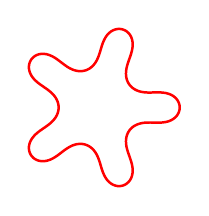
\begin{tikzpicture}[scale=0.45]

  \begin{axis}[
    hide axis,
    axis equal image,
    xmin = -1.42,
    xmax = 1.42,
    ymin = -1.42,
    ymax = 1.42,
    xtick = \empty,
    ytick = \empty,
    title style={align=left},
%    title={\Large $t = 2.99 \times 10^{-2}$ \\ \\ \Large $\nu = 0.38$}
  ]

\addplot[red,line width=2pt] coordinates{
(1.1542e+00,-1.5683e-12)
(1.1521e+00,2.7715e-02)
(1.1455e+00,5.5460e-02)
(1.1342e+00,8.3060e-02)
(1.1178e+00,1.1001e-01)
(1.0958e+00,1.3550e-01)
(1.0683e+00,1.5849e-01)
(1.0358e+00,1.7798e-01)
(9.9887e-01,1.9322e-01)
(9.5866e-01,2.0389e-01)
(9.1618e-01,2.1021e-01)
(8.7237e-01,2.1289e-01)
(8.2802e-01,2.1300e-01)
(7.8370e-01,2.1188e-01)
(7.3992e-01,2.1090e-01)
(6.9718e-01,2.1133e-01)
(6.5612e-01,2.1417e-01)
(6.1746e-01,2.2002e-01)
(5.8201e-01,2.2898e-01)
(5.5047e-01,2.4064e-01)
(5.2334e-01,2.5420e-01)
(5.0081e-01,2.6862e-01)
(4.8274e-01,2.8284e-01)
(4.6868e-01,2.9600e-01)
(4.5795e-01,3.0761e-01)
(4.4962e-01,3.1777e-01)
(4.4254e-01,3.2742e-01)
(4.3553e-01,3.3808e-01)
(4.2794e-01,3.5124e-01)
(4.1981e-01,3.6790e-01)
(4.1176e-01,3.8863e-01)
(4.0468e-01,4.1366e-01)
(3.9964e-01,4.4286e-01)
(3.9760e-01,4.7578e-01)
(3.9926e-01,5.1176e-01)
(4.0486e-01,5.4998e-01)
(4.1418e-01,5.8969e-01)
(4.2649e-01,6.3032e-01)
(4.4073e-01,6.7156e-01)
(4.5554e-01,7.1327e-01)
(4.6949e-01,7.5542e-01)
(4.8111e-01,7.9787e-01)
(4.8909e-01,8.4030e-01)
(4.9239e-01,8.8207e-01)
(4.9039e-01,9.2230e-01)
(4.8297e-01,9.5992e-01)
(4.7051e-01,9.9397e-01)
(4.5380e-01,1.0237e+00)
(4.3380e-01,1.0486e+00)
(4.1143e-01,1.0688e+00)
(3.8735e-01,1.0845e+00)
(3.6191e-01,1.0959e+00)
(3.3516e-01,1.1033e+00)
(3.0704e-01,1.1065e+00)
(2.7755e-01,1.1052e+00)
(2.4697e-01,1.0990e+00)
(2.1593e-01,1.0871e+00)
(1.8536e-01,1.0693e+00)
(1.5633e-01,1.0455e+00)
(1.2983e-01,1.0162e+00)
(1.0657e-01,9.8205e-01)
(8.6754e-02,9.4421e-01)
(7.0115e-02,9.0377e-01)
(5.5924e-02,8.6180e-01)
(4.3149e-02,8.1930e-01)
(3.0636e-02,7.7718e-01)
(1.7298e-02,7.3631e-01)
(2.3040e-03,6.9759e-01)
(-1.4778e-02,6.6193e-01)
(-3.3895e-02,6.3012e-01)
(-5.4525e-02,6.0278e-01)
(-7.5796e-02,5.8022e-01)
(-9.6673e-02,5.6235e-01)
(-1.1616e-01,5.4877e-01)
(-1.3351e-01,5.3883e-01)
(-1.4836e-01,5.3174e-01)
(-1.6095e-01,5.2666e-01)
(-1.7236e-01,5.2276e-01)
(-1.8433e-01,5.1934e-01)
(-1.9858e-01,5.1613e-01)
(-2.1619e-01,5.1339e-01)
(-2.3762e-01,5.1180e-01)
(-2.6288e-01,5.1228e-01)
(-2.9158e-01,5.1579e-01)
(-3.2307e-01,5.2317e-01)
(-3.5650e-01,5.3496e-01)
(-3.9099e-01,5.5123e-01)
(-4.2586e-01,5.7162e-01)
(-4.6072e-01,5.9535e-01)
(-4.9553e-01,6.2132e-01)
(-5.3053e-01,6.4828e-01)
(-5.6614e-01,6.7481e-01)
(-6.0270e-01,6.9952e-01)
(-6.4038e-01,7.2102e-01)
(-6.7896e-01,7.3808e-01)
(-7.1787e-01,7.4976e-01)
(-7.5619e-01,7.5553e-01)
(-7.9288e-01,7.5536e-01)
(-8.2692e-01,7.4966e-01)
(-8.5758e-01,7.3921e-01)
(-8.8447e-01,7.2485e-01)
(-9.0755e-01,7.0735e-01)
(-9.2697e-01,6.8718e-01)
(-9.4291e-01,6.6451e-01)
(-9.5538e-01,6.3929e-01)
(-9.6411e-01,6.1140e-01)
(-9.6854e-01,5.8087e-01)
(-9.6795e-01,5.4807e-01)
(-9.6166e-01,5.1369e-01)
(-9.4925e-01,4.7872e-01)
(-9.3072e-01,4.4424e-01)
(-9.0651e-01,4.1119e-01)
(-8.7748e-01,3.8021e-01)
(-8.4475e-01,3.5146e-01)
(-8.0956e-01,3.2467e-01)
(-7.7318e-01,2.9922e-01)
(-7.3683e-01,2.7429e-01)
(-7.0170e-01,2.4911e-01)
(-6.6892e-01,2.2309e-01)
(-6.3950e-01,1.9602e-01)
(-6.1425e-01,1.6811e-01)
(-5.9367e-01,1.3999e-01)
(-5.7786e-01,1.1254e-01)
(-5.6649e-01,8.6721e-02)
(-5.5894e-01,6.3407e-02)
(-5.5435e-01,4.3180e-02)
(-5.5187e-01,2.6233e-02)
(-5.5074e-01,1.2209e-02)
(-5.5043e-01,1.8275e-12)
(-5.5074e-01,-1.2209e-02)
(-5.5187e-01,-2.6233e-02)
(-5.5435e-01,-4.3180e-02)
(-5.5894e-01,-6.3407e-02)
(-5.6649e-01,-8.6721e-02)
(-5.7786e-01,-1.1254e-01)
(-5.9367e-01,-1.3999e-01)
(-6.1425e-01,-1.6811e-01)
(-6.3950e-01,-1.9602e-01)
(-6.6892e-01,-2.2309e-01)
(-7.0170e-01,-2.4911e-01)
(-7.3683e-01,-2.7429e-01)
(-7.7318e-01,-2.9922e-01)
(-8.0956e-01,-3.2467e-01)
(-8.4475e-01,-3.5146e-01)
(-8.7748e-01,-3.8021e-01)
(-9.0651e-01,-4.1119e-01)
(-9.3072e-01,-4.4424e-01)
(-9.4925e-01,-4.7872e-01)
(-9.6166e-01,-5.1369e-01)
(-9.6795e-01,-5.4807e-01)
(-9.6854e-01,-5.8087e-01)
(-9.6411e-01,-6.1140e-01)
(-9.5538e-01,-6.3929e-01)
(-9.4291e-01,-6.6451e-01)
(-9.2697e-01,-6.8718e-01)
(-9.0755e-01,-7.0735e-01)
(-8.8447e-01,-7.2485e-01)
(-8.5758e-01,-7.3921e-01)
(-8.2692e-01,-7.4966e-01)
(-7.9288e-01,-7.5536e-01)
(-7.5619e-01,-7.5553e-01)
(-7.1787e-01,-7.4976e-01)
(-6.7896e-01,-7.3808e-01)
(-6.4038e-01,-7.2102e-01)
(-6.0270e-01,-6.9952e-01)
(-5.6614e-01,-6.7481e-01)
(-5.3053e-01,-6.4828e-01)
(-4.9553e-01,-6.2132e-01)
(-4.6072e-01,-5.9535e-01)
(-4.2586e-01,-5.7162e-01)
(-3.9099e-01,-5.5123e-01)
(-3.5650e-01,-5.3496e-01)
(-3.2307e-01,-5.2317e-01)
(-2.9158e-01,-5.1579e-01)
(-2.6288e-01,-5.1228e-01)
(-2.3762e-01,-5.1180e-01)
(-2.1619e-01,-5.1339e-01)
(-1.9858e-01,-5.1613e-01)
(-1.8433e-01,-5.1934e-01)
(-1.7236e-01,-5.2276e-01)
(-1.6095e-01,-5.2666e-01)
(-1.4836e-01,-5.3174e-01)
(-1.3351e-01,-5.3883e-01)
(-1.1616e-01,-5.4877e-01)
(-9.6673e-02,-5.6235e-01)
(-7.5796e-02,-5.8022e-01)
(-5.4525e-02,-6.0278e-01)
(-3.3895e-02,-6.3012e-01)
(-1.4778e-02,-6.6193e-01)
(2.3040e-03,-6.9759e-01)
(1.7298e-02,-7.3631e-01)
(3.0636e-02,-7.7718e-01)
(4.3149e-02,-8.1930e-01)
(5.5924e-02,-8.6180e-01)
(7.0115e-02,-9.0377e-01)
(8.6754e-02,-9.4421e-01)
(1.0657e-01,-9.8205e-01)
(1.2983e-01,-1.0162e+00)
(1.5633e-01,-1.0455e+00)
(1.8536e-01,-1.0693e+00)
(2.1593e-01,-1.0871e+00)
(2.4697e-01,-1.0990e+00)
(2.7755e-01,-1.1052e+00)
(3.0704e-01,-1.1065e+00)
(3.3516e-01,-1.1033e+00)
(3.6191e-01,-1.0959e+00)
(3.8735e-01,-1.0845e+00)
(4.1143e-01,-1.0688e+00)
(4.3380e-01,-1.0486e+00)
(4.5380e-01,-1.0237e+00)
(4.7051e-01,-9.9397e-01)
(4.8297e-01,-9.5992e-01)
(4.9039e-01,-9.2230e-01)
(4.9239e-01,-8.8207e-01)
(4.8909e-01,-8.4030e-01)
(4.8111e-01,-7.9787e-01)
(4.6949e-01,-7.5542e-01)
(4.5554e-01,-7.1327e-01)
(4.4073e-01,-6.7156e-01)
(4.2649e-01,-6.3032e-01)
(4.1418e-01,-5.8969e-01)
(4.0486e-01,-5.4998e-01)
(3.9926e-01,-5.1176e-01)
(3.9760e-01,-4.7578e-01)
(3.9964e-01,-4.4286e-01)
(4.0468e-01,-4.1366e-01)
(4.1176e-01,-3.8863e-01)
(4.1981e-01,-3.6790e-01)
(4.2794e-01,-3.5124e-01)
(4.3553e-01,-3.3808e-01)
(4.4254e-01,-3.2742e-01)
(4.4962e-01,-3.1777e-01)
(4.5795e-01,-3.0761e-01)
(4.6868e-01,-2.9600e-01)
(4.8274e-01,-2.8284e-01)
(5.0081e-01,-2.6862e-01)
(5.2334e-01,-2.5420e-01)
(5.5047e-01,-2.4064e-01)
(5.8201e-01,-2.2898e-01)
(6.1746e-01,-2.2002e-01)
(6.5612e-01,-2.1417e-01)
(6.9718e-01,-2.1133e-01)
(7.3992e-01,-2.1090e-01)
(7.8370e-01,-2.1188e-01)
(8.2802e-01,-2.1300e-01)
(8.7237e-01,-2.1289e-01)
(9.1618e-01,-2.1021e-01)
(9.5866e-01,-2.0389e-01)
(9.9887e-01,-1.9322e-01)
(1.0358e+00,-1.7798e-01)
(1.0683e+00,-1.5849e-01)
(1.0958e+00,-1.3550e-01)
(1.1178e+00,-1.1001e-01)
(1.1342e+00,-8.3060e-02)
(1.1455e+00,-5.5460e-02)
(1.1521e+00,-2.7715e-02)
(1.1542e+00,-1.5683e-12)
};


\end{axis}

\end{tikzpicture}

%    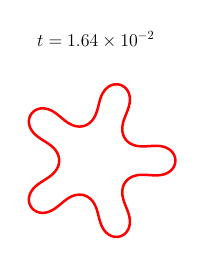
\begin{tikzpicture}[scale=0.45]

  \begin{axis}[
    hide axis,
    axis equal image,
    xmin = -2.1,
    xmax = 2.1,
    ymin = -2.1,
    ymax = 2.1,
    xtick = \empty,
    ytick = \empty,
    title style={align=left},
    title={\Large $t = 1.64 \times 10^{-2}$}
  ]

\addplot[red,line width=2pt] coordinates{
(1.6571e+00,-2.4995e-13)
(1.6540e+00,4.0568e-02)
(1.6446e+00,8.1200e-02)
(1.6282e+00,1.2166e-01)
(1.6043e+00,1.6121e-01)
(1.5722e+00,1.9863e-01)
(1.5321e+00,2.3234e-01)
(1.4844e+00,2.6078e-01)
(1.4303e+00,2.8269e-01)
(1.3712e+00,2.9752e-01)
(1.3088e+00,3.0550e-01)
(1.2447e+00,3.0765e-01)
(1.1798e+00,3.0562e-01)
(1.1150e+00,3.0146e-01)
(1.0511e+00,2.9730e-01)
(9.8855e-01,2.9516e-01)
(9.2832e-01,2.9667e-01)
(8.7143e-01,3.0283e-01)
(8.1907e-01,3.1391e-01)
(7.7235e-01,3.2939e-01)
(7.3210e-01,3.4809e-01)
(6.9865e-01,3.6843e-01)
(6.7184e-01,3.8879e-01)
(6.5103e-01,4.0781e-01)
(6.3518e-01,4.2470e-01)
(6.2292e-01,4.3956e-01)
(6.1255e-01,4.5367e-01)
(6.0232e-01,4.6933e-01)
(5.9132e-01,4.8869e-01)
(5.7970e-01,5.1321e-01)
(5.6840e-01,5.4374e-01)
(5.5884e-01,5.8058e-01)
(5.5264e-01,6.2350e-01)
(5.5125e-01,6.7177e-01)
(5.5567e-01,7.2429e-01)
(5.6620e-01,7.7984e-01)
(5.8238e-01,8.3730e-01)
(6.0302e-01,8.9592e-01)
(6.2643e-01,9.5532e-01)
(6.5053e-01,1.0155e+00)
(6.7308e-01,1.0764e+00)
(6.9187e-01,1.1380e+00)
(7.0491e-01,1.1998e+00)
(7.1065e-01,1.2609e+00)
(7.0821e-01,1.3198e+00)
(6.9750e-01,1.3749e+00)
(6.7921e-01,1.4247e+00)
(6.5461e-01,1.4681e+00)
(6.2519e-01,1.5045e+00)
(5.9232e-01,1.5339e+00)
(5.5701e-01,1.5567e+00)
(5.1976e-01,1.5734e+00)
(4.8061e-01,1.5842e+00)
(4.3946e-01,1.5890e+00)
(3.9629e-01,1.5873e+00)
(3.5151e-01,1.5783e+00)
(3.0601e-01,1.5611e+00)
(2.6120e-01,1.5352e+00)
(2.1875e-01,1.5003e+00)
(1.8023e-01,1.4572e+00)
(1.4679e-01,1.4068e+00)
(1.1886e-01,1.3509e+00)
(9.6059e-02,1.2911e+00)
(7.7305e-02,1.2290e+00)
(6.0987e-02,1.1662e+00)
(4.5272e-02,1.1038e+00)
(2.8403e-02,1.0432e+00)
(8.9895e-03,9.8560e-01)
(-1.3754e-02,9.3237e-01)
(-3.9864e-02,8.8474e-01)
(-6.8632e-02,8.4370e-01)
(-9.8765e-02,8.0976e-01)
(-1.2869e-01,7.8288e-01)
(-1.5685e-01,7.6249e-01)
(-1.8205e-01,7.4761e-01)
(-2.0372e-01,7.3704e-01)
(-2.2214e-01,7.2952e-01)
(-2.3883e-01,7.2379e-01)
(-2.5638e-01,7.1883e-01)
(-2.7730e-01,7.1424e-01)
(-3.0312e-01,7.1049e-01)
(-3.3453e-01,7.0863e-01)
(-3.7147e-01,7.1008e-01)
(-4.1334e-01,7.1633e-01)
(-4.5905e-01,7.2861e-01)
(-5.0730e-01,7.4766e-01)
(-5.5676e-01,7.7353e-01)
(-6.0644e-01,8.0557e-01)
(-6.5587e-01,8.4253e-01)
(-7.0512e-01,8.8272e-01)
(-7.5471e-01,9.2421e-01)
(-8.0539e-01,9.6491e-01)
(-8.5779e-01,1.0027e+00)
(-9.1218e-01,1.0354e+00)
(-9.6824e-01,1.0613e+00)
(-1.0250e+00,1.0789e+00)
(-1.0811e+00,1.0876e+00)
(-1.1348e+00,1.0873e+00)
(-1.1845e+00,1.0788e+00)
(-1.2294e+00,1.0633e+00)
(-1.2686e+00,1.0422e+00)
(-1.3023e+00,1.0164e+00)
(-1.3307e+00,9.8687e-01)
(-1.3541e+00,9.5370e-01)
(-1.3724e+00,9.1682e-01)
(-1.3853e+00,8.7603e-01)
(-1.3920e+00,8.3139e-01)
(-1.3913e+00,7.8337e-01)
(-1.3822e+00,7.3304e-01)
(-1.3640e+00,6.8186e-01)
(-1.3367e+00,6.3152e-01)
(-1.3007e+00,5.8355e-01)
(-1.2574e+00,5.3896e-01)
(-1.2085e+00,4.9808e-01)
(-1.1558e+00,4.6051e-01)
(-1.1012e+00,4.2525e-01)
(-1.0466e+00,3.9099e-01)
(-9.9359e-01,3.5642e-01)
(-9.4396e-01,3.2051e-01)
(-8.9923e-01,2.8279e-01)
(-8.6065e-01,2.4347e-01)
(-8.2907e-01,2.0343e-01)
(-8.0469e-01,1.6398e-01)
(-7.8711e-01,1.2663e-01)
(-7.7539e-01,9.2723e-02)
(-7.6827e-01,6.3215e-02)
(-7.6441e-01,3.8427e-02)
(-7.6264e-01,1.7877e-02)
(-7.6216e-01,-1.0277e-13)
(-7.6264e-01,-1.7877e-02)
(-7.6441e-01,-3.8427e-02)
(-7.6827e-01,-6.3215e-02)
(-7.7539e-01,-9.2723e-02)
(-7.8711e-01,-1.2663e-01)
(-8.0469e-01,-1.6398e-01)
(-8.2907e-01,-2.0343e-01)
(-8.6065e-01,-2.4347e-01)
(-8.9923e-01,-2.8279e-01)
(-9.4396e-01,-3.2051e-01)
(-9.9359e-01,-3.5642e-01)
(-1.0466e+00,-3.9099e-01)
(-1.1012e+00,-4.2525e-01)
(-1.1558e+00,-4.6051e-01)
(-1.2085e+00,-4.9808e-01)
(-1.2574e+00,-5.3896e-01)
(-1.3007e+00,-5.8355e-01)
(-1.3367e+00,-6.3152e-01)
(-1.3640e+00,-6.8186e-01)
(-1.3822e+00,-7.3304e-01)
(-1.3913e+00,-7.8337e-01)
(-1.3920e+00,-8.3139e-01)
(-1.3853e+00,-8.7603e-01)
(-1.3724e+00,-9.1682e-01)
(-1.3541e+00,-9.5370e-01)
(-1.3307e+00,-9.8687e-01)
(-1.3023e+00,-1.0164e+00)
(-1.2686e+00,-1.0422e+00)
(-1.2294e+00,-1.0633e+00)
(-1.1845e+00,-1.0788e+00)
(-1.1348e+00,-1.0873e+00)
(-1.0811e+00,-1.0876e+00)
(-1.0250e+00,-1.0789e+00)
(-9.6824e-01,-1.0613e+00)
(-9.1218e-01,-1.0354e+00)
(-8.5779e-01,-1.0027e+00)
(-8.0539e-01,-9.6491e-01)
(-7.5471e-01,-9.2421e-01)
(-7.0512e-01,-8.8272e-01)
(-6.5587e-01,-8.4253e-01)
(-6.0644e-01,-8.0557e-01)
(-5.5676e-01,-7.7353e-01)
(-5.0730e-01,-7.4766e-01)
(-4.5905e-01,-7.2861e-01)
(-4.1334e-01,-7.1633e-01)
(-3.7147e-01,-7.1008e-01)
(-3.3453e-01,-7.0863e-01)
(-3.0312e-01,-7.1049e-01)
(-2.7730e-01,-7.1424e-01)
(-2.5638e-01,-7.1883e-01)
(-2.3883e-01,-7.2379e-01)
(-2.2214e-01,-7.2952e-01)
(-2.0372e-01,-7.3704e-01)
(-1.8205e-01,-7.4761e-01)
(-1.5685e-01,-7.6249e-01)
(-1.2869e-01,-7.8288e-01)
(-9.8765e-02,-8.0976e-01)
(-6.8632e-02,-8.4370e-01)
(-3.9864e-02,-8.8474e-01)
(-1.3754e-02,-9.3237e-01)
(8.9895e-03,-9.8560e-01)
(2.8403e-02,-1.0432e+00)
(4.5272e-02,-1.1038e+00)
(6.0987e-02,-1.1662e+00)
(7.7305e-02,-1.2290e+00)
(9.6059e-02,-1.2911e+00)
(1.1886e-01,-1.3509e+00)
(1.4679e-01,-1.4068e+00)
(1.8023e-01,-1.4572e+00)
(2.1875e-01,-1.5003e+00)
(2.6120e-01,-1.5352e+00)
(3.0601e-01,-1.5611e+00)
(3.5151e-01,-1.5783e+00)
(3.9629e-01,-1.5873e+00)
(4.3946e-01,-1.5890e+00)
(4.8061e-01,-1.5842e+00)
(5.1976e-01,-1.5734e+00)
(5.5701e-01,-1.5567e+00)
(5.9232e-01,-1.5339e+00)
(6.2519e-01,-1.5045e+00)
(6.5461e-01,-1.4681e+00)
(6.7921e-01,-1.4247e+00)
(6.9750e-01,-1.3749e+00)
(7.0821e-01,-1.3198e+00)
(7.1065e-01,-1.2609e+00)
(7.0491e-01,-1.1998e+00)
(6.9187e-01,-1.1380e+00)
(6.7308e-01,-1.0764e+00)
(6.5053e-01,-1.0155e+00)
(6.2643e-01,-9.5532e-01)
(6.0302e-01,-8.9592e-01)
(5.8238e-01,-8.3730e-01)
(5.6620e-01,-7.7984e-01)
(5.5567e-01,-7.2429e-01)
(5.5125e-01,-6.7177e-01)
(5.5264e-01,-6.2350e-01)
(5.5884e-01,-5.8058e-01)
(5.6840e-01,-5.4374e-01)
(5.7970e-01,-5.1321e-01)
(5.9132e-01,-4.8869e-01)
(6.0232e-01,-4.6933e-01)
(6.1255e-01,-4.5367e-01)
(6.2292e-01,-4.3956e-01)
(6.3518e-01,-4.2470e-01)
(6.5103e-01,-4.0781e-01)
(6.7184e-01,-3.8879e-01)
(6.9865e-01,-3.6843e-01)
(7.3210e-01,-3.4809e-01)
(7.7235e-01,-3.2939e-01)
(8.1907e-01,-3.1391e-01)
(8.7143e-01,-3.0283e-01)
(9.2832e-01,-2.9667e-01)
(9.8855e-01,-2.9516e-01)
(1.0511e+00,-2.9730e-01)
(1.1150e+00,-3.0146e-01)
(1.1798e+00,-3.0562e-01)
(1.2447e+00,-3.0765e-01)
(1.3088e+00,-3.0550e-01)
(1.3712e+00,-2.9752e-01)
(1.4303e+00,-2.8269e-01)
(1.4844e+00,-2.6078e-01)
(1.5321e+00,-2.3234e-01)
(1.5722e+00,-1.9863e-01)
(1.6043e+00,-1.6121e-01)
(1.6282e+00,-1.2166e-01)
(1.6446e+00,-8.1200e-02)
(1.6540e+00,-4.0568e-02)
(1.6571e+00,-2.4995e-13)
};



\end{axis}

\end{tikzpicture}

%    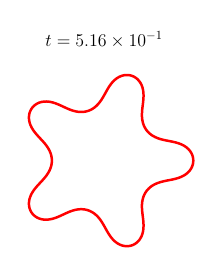
\begin{tikzpicture}[scale=0.45]

  \begin{axis}[
    hide axis,
    axis equal image,
    xmin = -2.1,
    xmax = 2.1,
    ymin = -2.1,
    ymax = 2.1,
    xtick = \empty,
    ytick = \empty,
    title style={align=left},
    title={\Large $t = 5.16 \times 10^{-1}$}
  ]

\addplot[red,line width=2pt] coordinates{
(1.8573e+00,-9.0339e-12)
(1.8547e+00,4.0614e-02)
(1.8468e+00,8.1577e-02)
(1.8329e+00,1.2298e-01)
(1.8125e+00,1.6450e-01)
(1.7849e+00,2.0534e-01)
(1.7499e+00,2.4438e-01)
(1.7076e+00,2.8039e-01)
(1.6587e+00,3.1229e-01)
(1.6042e+00,3.3941e-01)
(1.5454e+00,3.6165e-01)
(1.4837e+00,3.7953e-01)
(1.4204e+00,3.9408e-01)
(1.3568e+00,4.0669e-01)
(1.2938e+00,4.1888e-01)
(1.2327e+00,4.3205e-01)
(1.1744e+00,4.4730e-01)
(1.1200e+00,4.6519e-01)
(1.0706e+00,4.8573e-01)
(1.0269e+00,5.0836e-01)
(9.8935e-01,5.3209e-01)
(9.5812e-01,5.5570e-01)
(9.3291e-01,5.7802e-01)
(9.1310e-01,5.9809e-01)
(8.9780e-01,6.1548e-01)
(8.8578e-01,6.3053e-01)
(8.7542e-01,6.4466e-01)
(8.6500e-01,6.6019e-01)
(8.5345e-01,6.7922e-01)
(8.4067e-01,7.0316e-01)
(8.2726e-01,7.3284e-01)
(8.1423e-01,7.6861e-01)
(8.0279e-01,8.1045e-01)
(7.9411e-01,8.5796e-01)
(7.8906e-01,9.1044e-01)
(7.8804e-01,9.6697e-01)
(7.9086e-01,1.0266e+00)
(7.9675e-01,1.0885e+00)
(8.0444e-01,1.1519e+00)
(8.1229e-01,1.2162e+00)
(8.1853e-01,1.2808e+00)
(8.2145e-01,1.3452e+00)
(8.1957e-01,1.4084e+00)
(8.1186e-01,1.4692e+00)
(7.9790e-01,1.5265e+00)
(7.7786e-01,1.5789e+00)
(7.5249e-01,1.6256e+00)
(7.2287e-01,1.6657e+00)
(6.9018e-01,1.6993e+00)
(6.5541e-01,1.7264e+00)
(6.1917e-01,1.7478e+00)
(5.8162e-01,1.7638e+00)
(5.4255e-01,1.7749e+00)
(5.0156e-01,1.7810e+00)
(4.5835e-01,1.7817e+00)
(4.1296e-01,1.7765e+00)
(3.6585e-01,1.7643e+00)
(3.1792e-01,1.7447e+00)
(2.7038e-01,1.7172e+00)
(2.2445e-01,1.6819e+00)
(1.8119e-01,1.6397e+00)
(1.4119e-01,1.5917e+00)
(1.0450e-01,1.5392e+00)
(7.0641e-02,1.4839e+00)
(3.8719e-02,1.4274e+00)
(7.6439e-03,1.3711e+00)
(-2.3635e-02,1.3165e+00)
(-5.5892e-02,1.2650e+00)
(-8.9454e-02,1.2178e+00)
(-1.2412e-01,1.1760e+00)
(-1.5918e-01,1.1401e+00)
(-1.9361e-01,1.1105e+00)
(-2.2623e-01,1.0870e+00)
(-2.5593e-01,1.0689e+00)
(-2.8193e-01,1.0555e+00)
(-3.0396e-01,1.0457e+00)
(-3.2253e-01,1.0385e+00)
(-3.3924e-01,1.0328e+00)
(-3.5674e-01,1.0277e+00)
(-3.7754e-01,1.0226e+00)
(-4.0318e-01,1.0177e+00)
(-4.3440e-01,1.0138e+00)
(-4.7133e-01,1.0119e+00)
(-5.1365e-01,1.0132e+00)
(-5.6068e-01,1.0187e+00)
(-6.1151e-01,1.0291e+00)
(-6.6515e-01,1.0446e+00)
(-7.2070e-01,1.0648e+00)
(-7.7752e-01,1.0890e+00)
(-8.3526e-01,1.1155e+00)
(-8.9383e-01,1.1429e+00)
(-9.5324e-01,1.1693e+00)
(-1.0134e+00,1.1928e+00)
(-1.0741e+00,1.2116e+00)
(-1.1345e+00,1.2244e+00)
(-1.1936e+00,1.2303e+00)
(-1.2504e+00,1.2289e+00)
(-1.3034e+00,1.2204e+00)
(-1.3518e+00,1.2058e+00)
(-1.3949e+00,1.1860e+00)
(-1.4325e+00,1.1620e+00)
(-1.4650e+00,1.1348e+00)
(-1.4927e+00,1.1046e+00)
(-1.5161e+00,1.0715e+00)
(-1.5355e+00,1.0351e+00)
(-1.5505e+00,9.9499e-01)
(-1.5606e+00,9.5098e-01)
(-1.5649e+00,9.0314e-01)
(-1.5624e+00,8.5203e-01)
(-1.5525e+00,7.9862e-01)
(-1.5347e+00,7.4413e-01)
(-1.5094e+00,6.8978e-01)
(-1.4773e+00,6.3657e-01)
(-1.4397e+00,5.8510e-01)
(-1.3981e+00,5.3547e-01)
(-1.3544e+00,4.8738e-01)
(-1.3103e+00,4.4029e-01)
(-1.2676e+00,3.9364e-01)
(-1.2278e+00,3.4705e-01)
(-1.1923e+00,3.0051e-01)
(-1.1621e+00,2.5444e-01)
(-1.1377e+00,2.0964e-01)
(-1.1191e+00,1.6716e-01)
(-1.1058e+00,1.2807e-01)
(-1.0970e+00,9.3280e-02)
(-1.0917e+00,6.3390e-02)
(-1.0888e+00,3.8466e-02)
(-1.0875e+00,1.7880e-02)
(-1.0871e+00,1.1759e-11)
(-1.0875e+00,-1.7880e-02)
(-1.0888e+00,-3.8466e-02)
(-1.0917e+00,-6.3390e-02)
(-1.0970e+00,-9.3280e-02)
(-1.1058e+00,-1.2807e-01)
(-1.1191e+00,-1.6716e-01)
(-1.1377e+00,-2.0964e-01)
(-1.1621e+00,-2.5444e-01)
(-1.1923e+00,-3.0051e-01)
(-1.2278e+00,-3.4705e-01)
(-1.2676e+00,-3.9364e-01)
(-1.3103e+00,-4.4029e-01)
(-1.3544e+00,-4.8738e-01)
(-1.3981e+00,-5.3547e-01)
(-1.4397e+00,-5.8510e-01)
(-1.4773e+00,-6.3657e-01)
(-1.5094e+00,-6.8978e-01)
(-1.5347e+00,-7.4413e-01)
(-1.5525e+00,-7.9862e-01)
(-1.5624e+00,-8.5203e-01)
(-1.5649e+00,-9.0314e-01)
(-1.5606e+00,-9.5098e-01)
(-1.5505e+00,-9.9499e-01)
(-1.5355e+00,-1.0351e+00)
(-1.5161e+00,-1.0715e+00)
(-1.4927e+00,-1.1046e+00)
(-1.4650e+00,-1.1348e+00)
(-1.4325e+00,-1.1620e+00)
(-1.3949e+00,-1.1860e+00)
(-1.3518e+00,-1.2058e+00)
(-1.3034e+00,-1.2204e+00)
(-1.2504e+00,-1.2289e+00)
(-1.1936e+00,-1.2303e+00)
(-1.1345e+00,-1.2244e+00)
(-1.0741e+00,-1.2116e+00)
(-1.0134e+00,-1.1928e+00)
(-9.5324e-01,-1.1693e+00)
(-8.9383e-01,-1.1429e+00)
(-8.3526e-01,-1.1155e+00)
(-7.7752e-01,-1.0890e+00)
(-7.2070e-01,-1.0648e+00)
(-6.6515e-01,-1.0446e+00)
(-6.1151e-01,-1.0291e+00)
(-5.6068e-01,-1.0187e+00)
(-5.1365e-01,-1.0132e+00)
(-4.7133e-01,-1.0119e+00)
(-4.3440e-01,-1.0138e+00)
(-4.0318e-01,-1.0177e+00)
(-3.7754e-01,-1.0226e+00)
(-3.5674e-01,-1.0277e+00)
(-3.3924e-01,-1.0328e+00)
(-3.2253e-01,-1.0385e+00)
(-3.0396e-01,-1.0457e+00)
(-2.8193e-01,-1.0555e+00)
(-2.5593e-01,-1.0689e+00)
(-2.2623e-01,-1.0870e+00)
(-1.9361e-01,-1.1105e+00)
(-1.5918e-01,-1.1401e+00)
(-1.2412e-01,-1.1760e+00)
(-8.9454e-02,-1.2178e+00)
(-5.5892e-02,-1.2650e+00)
(-2.3635e-02,-1.3165e+00)
(7.6439e-03,-1.3711e+00)
(3.8719e-02,-1.4274e+00)
(7.0641e-02,-1.4839e+00)
(1.0450e-01,-1.5392e+00)
(1.4119e-01,-1.5917e+00)
(1.8119e-01,-1.6397e+00)
(2.2445e-01,-1.6819e+00)
(2.7038e-01,-1.7172e+00)
(3.1792e-01,-1.7447e+00)
(3.6585e-01,-1.7643e+00)
(4.1296e-01,-1.7765e+00)
(4.5835e-01,-1.7817e+00)
(5.0156e-01,-1.7810e+00)
(5.4255e-01,-1.7749e+00)
(5.8162e-01,-1.7638e+00)
(6.1917e-01,-1.7478e+00)
(6.5541e-01,-1.7264e+00)
(6.9018e-01,-1.6993e+00)
(7.2287e-01,-1.6657e+00)
(7.5249e-01,-1.6256e+00)
(7.7786e-01,-1.5789e+00)
(7.9790e-01,-1.5265e+00)
(8.1186e-01,-1.4692e+00)
(8.1957e-01,-1.4084e+00)
(8.2145e-01,-1.3452e+00)
(8.1853e-01,-1.2808e+00)
(8.1229e-01,-1.2162e+00)
(8.0444e-01,-1.1519e+00)
(7.9675e-01,-1.0885e+00)
(7.9086e-01,-1.0266e+00)
(7.8804e-01,-9.6697e-01)
(7.8906e-01,-9.1044e-01)
(7.9411e-01,-8.5796e-01)
(8.0279e-01,-8.1045e-01)
(8.1423e-01,-7.6861e-01)
(8.2726e-01,-7.3284e-01)
(8.4067e-01,-7.0316e-01)
(8.5345e-01,-6.7922e-01)
(8.6500e-01,-6.6019e-01)
(8.7542e-01,-6.4466e-01)
(8.8578e-01,-6.3053e-01)
(8.9780e-01,-6.1548e-01)
(9.1310e-01,-5.9809e-01)
(9.3291e-01,-5.7802e-01)
(9.5812e-01,-5.5570e-01)
(9.8935e-01,-5.3209e-01)
(1.0269e+00,-5.0836e-01)
(1.0706e+00,-4.8573e-01)
(1.1200e+00,-4.6519e-01)
(1.1744e+00,-4.4730e-01)
(1.2327e+00,-4.3205e-01)
(1.2938e+00,-4.1888e-01)
(1.3568e+00,-4.0669e-01)
(1.4204e+00,-3.9408e-01)
(1.4837e+00,-3.7953e-01)
(1.5454e+00,-3.6165e-01)
(1.6042e+00,-3.3941e-01)
(1.6587e+00,-3.1229e-01)
(1.7076e+00,-2.8039e-01)
(1.7499e+00,-2.4438e-01)
(1.7849e+00,-2.0534e-01)
(1.8125e+00,-1.6450e-01)
(1.8329e+00,-1.2298e-01)
(1.8468e+00,-8.1577e-02)
(1.8547e+00,-4.0614e-02)
(1.8573e+00,-9.0339e-12)
};



\end{axis}

\end{tikzpicture}

%    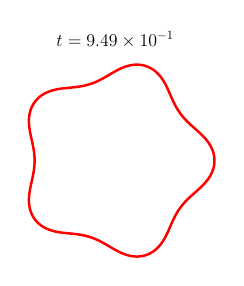
\begin{tikzpicture}[scale=0.45]

  \begin{axis}[
    hide axis,
    axis equal image,
    xmin = -2.1,
    xmax = 2.1,
    ymin = -2.1,
    ymax = 2.1,
    xtick = \empty,
    ytick = \empty,
    title style={align=left},
    title={\Large $t = 9.49 \times 10^{-1}$}
  ]

\addplot[red,line width=2pt] coordinates{
(2.0699e+00,-5.6473e-11)
(2.0685e+00,4.0691e-02)
(2.0641e+00,8.2211e-02)
(2.0564e+00,1.2521e-01)
(2.0450e+00,1.7005e-01)
(2.0292e+00,2.1674e-01)
(2.0085e+00,2.6499e-01)
(1.9828e+00,3.1424e-01)
(1.9519e+00,3.6386e-01)
(1.9161e+00,4.1317e-01)
(1.8760e+00,4.6160e-01)
(1.8324e+00,5.0875e-01)
(1.7863e+00,5.5443e-01)
(1.7387e+00,5.9859e-01)
(1.6909e+00,6.4131e-01)
(1.6440e+00,6.8270e-01)
(1.5990e+00,7.2276e-01)
(1.5568e+00,7.6141e-01)
(1.5181e+00,7.9839e-01)
(1.4833e+00,8.3329e-01)
(1.4529e+00,8.6561e-01)
(1.4268e+00,8.9485e-01)
(1.4051e+00,9.2056e-01)
(1.3873e+00,9.4249e-01)
(1.3731e+00,9.6079e-01)
(1.3616e+00,9.7620e-01)
(1.3513e+00,9.9036e-01)
(1.3405e+00,1.0056e+00)
(1.3279e+00,1.0240e+00)
(1.3130e+00,1.0467e+00)
(1.2957e+00,1.0743e+00)
(1.2763e+00,1.1071e+00)
(1.2553e+00,1.1450e+00)
(1.2330e+00,1.1879e+00)
(1.2099e+00,1.2353e+00)
(1.1863e+00,1.2867e+00)
(1.1622e+00,1.3413e+00)
(1.1375e+00,1.3984e+00)
(1.1119e+00,1.4568e+00)
(1.0849e+00,1.5157e+00)
(1.0561e+00,1.5740e+00)
(1.0252e+00,1.6305e+00)
(9.9198e-01,1.6843e+00)
(9.5655e-01,1.7344e+00)
(9.1923e-01,1.7800e+00)
(8.8054e-01,1.8208e+00)
(8.4111e-01,1.8563e+00)
(8.0155e-01,1.8868e+00)
(7.6235e-01,1.9125e+00)
(7.2371e-01,1.9338e+00)
(6.8552e-01,1.9515e+00)
(6.4734e-01,1.9660e+00)
(6.0845e-01,1.9777e+00)
(5.6801e-01,1.9869e+00)
(5.2528e-01,1.9935e+00)
(4.7970e-01,1.9971e+00)
(4.3103e-01,1.9972e+00)
(3.7934e-01,1.9934e+00)
(3.2500e-01,1.9851e+00)
(2.6860e-01,1.9720e+00)
(2.1083e-01,1.9542e+00)
(1.5243e-01,1.9318e+00)
(9.4027e-02,1.9056e+00)
(3.6168e-02,1.8763e+00)
(-2.0752e-02,1.8450e+00)
(-7.6433e-02,1.8129e+00)
(-1.3062e-01,1.7809e+00)
(-1.8303e-01,1.7501e+00)
(-2.3332e-01,1.7214e+00)
(-2.8103e-01,1.6954e+00)
(-3.2564e-01,1.6725e+00)
(-3.6659e-01,1.6529e+00)
(-4.0334e-01,1.6365e+00)
(-4.3548e-01,1.6232e+00)
(-4.6277e-01,1.6126e+00)
(-4.8543e-01,1.6043e+00)
(-5.0424e-01,1.5978e+00)
(-5.2100e-01,1.5923e+00)
(-5.3840e-01,1.5868e+00)
(-5.5893e-01,1.5807e+00)
(-5.8408e-01,1.5737e+00)
(-6.1457e-01,1.5660e+00)
(-6.5062e-01,1.5577e+00)
(-6.9215e-01,1.5494e+00)
(-7.3882e-01,1.5413e+00)
(-7.9018e-01,1.5339e+00)
(-8.4562e-01,1.5272e+00)
(-9.0443e-01,1.5210e+00)
(-9.6588e-01,1.5152e+00)
(-1.0291e+00,1.5090e+00)
(-1.0934e+00,1.5018e+00)
(-1.1578e+00,1.4929e+00)
(-1.2214e+00,1.4815e+00)
(-1.2832e+00,1.4672e+00)
(-1.3424e+00,1.4496e+00)
(-1.3982e+00,1.4288e+00)
(-1.4498e+00,1.4051e+00)
(-1.4967e+00,1.3790e+00)
(-1.5389e+00,1.3511e+00)
(-1.5763e+00,1.3219e+00)
(-1.6094e+00,1.2919e+00)
(-1.6387e+00,1.2612e+00)
(-1.6648e+00,1.2296e+00)
(-1.6884e+00,1.1966e+00)
(-1.7100e+00,1.1615e+00)
(-1.7298e+00,1.1236e+00)
(-1.7478e+00,1.0821e+00)
(-1.7635e+00,1.0367e+00)
(-1.7764e+00,9.8714e-01)
(-1.7860e+00,9.3364e-01)
(-1.7918e+00,8.7660e-01)
(-1.7935e+00,8.1664e-01)
(-1.7911e+00,7.5452e-01)
(-1.7849e+00,6.9105e-01)
(-1.7755e+00,6.2701e-01)
(-1.7637e+00,5.6310e-01)
(-1.7505e+00,4.9997e-01)
(-1.7368e+00,4.3821e-01)
(-1.7236e+00,3.7839e-01)
(-1.7115e+00,3.2111e-01)
(-1.7011e+00,2.6699e-01)
(-1.6927e+00,2.1666e-01)
(-1.6863e+00,1.7071e-01)
(-1.6818e+00,1.2966e-01)
(-1.6788e+00,9.3894e-02)
(-1.6770e+00,6.3583e-02)
(-1.6760e+00,3.8509e-02)
(-1.6755e+00,1.7885e-02)
(-1.6754e+00,-9.7486e-12)
(-1.6755e+00,-1.7885e-02)
(-1.6760e+00,-3.8509e-02)
(-1.6770e+00,-6.3583e-02)
(-1.6788e+00,-9.3894e-02)
(-1.6818e+00,-1.2966e-01)
(-1.6863e+00,-1.7071e-01)
(-1.6927e+00,-2.1666e-01)
(-1.7011e+00,-2.6699e-01)
(-1.7115e+00,-3.2111e-01)
(-1.7236e+00,-3.7839e-01)
(-1.7368e+00,-4.3821e-01)
(-1.7505e+00,-4.9997e-01)
(-1.7637e+00,-5.6310e-01)
(-1.7755e+00,-6.2701e-01)
(-1.7849e+00,-6.9105e-01)
(-1.7911e+00,-7.5452e-01)
(-1.7935e+00,-8.1664e-01)
(-1.7918e+00,-8.7660e-01)
(-1.7860e+00,-9.3364e-01)
(-1.7764e+00,-9.8714e-01)
(-1.7635e+00,-1.0367e+00)
(-1.7478e+00,-1.0821e+00)
(-1.7298e+00,-1.1236e+00)
(-1.7100e+00,-1.1615e+00)
(-1.6884e+00,-1.1966e+00)
(-1.6648e+00,-1.2296e+00)
(-1.6387e+00,-1.2612e+00)
(-1.6094e+00,-1.2919e+00)
(-1.5763e+00,-1.3219e+00)
(-1.5389e+00,-1.3511e+00)
(-1.4967e+00,-1.3790e+00)
(-1.4498e+00,-1.4051e+00)
(-1.3982e+00,-1.4288e+00)
(-1.3424e+00,-1.4496e+00)
(-1.2832e+00,-1.4672e+00)
(-1.2214e+00,-1.4815e+00)
(-1.1578e+00,-1.4929e+00)
(-1.0934e+00,-1.5018e+00)
(-1.0291e+00,-1.5090e+00)
(-9.6588e-01,-1.5152e+00)
(-9.0443e-01,-1.5210e+00)
(-8.4562e-01,-1.5272e+00)
(-7.9018e-01,-1.5339e+00)
(-7.3882e-01,-1.5413e+00)
(-6.9215e-01,-1.5494e+00)
(-6.5062e-01,-1.5577e+00)
(-6.1457e-01,-1.5660e+00)
(-5.8408e-01,-1.5737e+00)
(-5.5893e-01,-1.5807e+00)
(-5.3840e-01,-1.5868e+00)
(-5.2100e-01,-1.5923e+00)
(-5.0424e-01,-1.5978e+00)
(-4.8543e-01,-1.6043e+00)
(-4.6277e-01,-1.6126e+00)
(-4.3548e-01,-1.6232e+00)
(-4.0334e-01,-1.6365e+00)
(-3.6659e-01,-1.6529e+00)
(-3.2564e-01,-1.6725e+00)
(-2.8103e-01,-1.6954e+00)
(-2.3332e-01,-1.7214e+00)
(-1.8303e-01,-1.7501e+00)
(-1.3062e-01,-1.7809e+00)
(-7.6433e-02,-1.8129e+00)
(-2.0752e-02,-1.8450e+00)
(3.6168e-02,-1.8763e+00)
(9.4027e-02,-1.9056e+00)
(1.5243e-01,-1.9318e+00)
(2.1083e-01,-1.9542e+00)
(2.6860e-01,-1.9720e+00)
(3.2500e-01,-1.9851e+00)
(3.7934e-01,-1.9934e+00)
(4.3103e-01,-1.9972e+00)
(4.7970e-01,-1.9971e+00)
(5.2528e-01,-1.9935e+00)
(5.6801e-01,-1.9869e+00)
(6.0845e-01,-1.9777e+00)
(6.4734e-01,-1.9660e+00)
(6.8552e-01,-1.9515e+00)
(7.2371e-01,-1.9338e+00)
(7.6235e-01,-1.9125e+00)
(8.0155e-01,-1.8868e+00)
(8.4111e-01,-1.8563e+00)
(8.8054e-01,-1.8208e+00)
(9.1923e-01,-1.7800e+00)
(9.5655e-01,-1.7344e+00)
(9.9198e-01,-1.6843e+00)
(1.0252e+00,-1.6305e+00)
(1.0561e+00,-1.5740e+00)
(1.0849e+00,-1.5157e+00)
(1.1119e+00,-1.4568e+00)
(1.1375e+00,-1.3984e+00)
(1.1622e+00,-1.3413e+00)
(1.1863e+00,-1.2867e+00)
(1.2099e+00,-1.2353e+00)
(1.2330e+00,-1.1879e+00)
(1.2553e+00,-1.1450e+00)
(1.2763e+00,-1.1071e+00)
(1.2957e+00,-1.0743e+00)
(1.3130e+00,-1.0467e+00)
(1.3279e+00,-1.0240e+00)
(1.3405e+00,-1.0056e+00)
(1.3513e+00,-9.9036e-01)
(1.3616e+00,-9.7620e-01)
(1.3731e+00,-9.6079e-01)
(1.3873e+00,-9.4249e-01)
(1.4051e+00,-9.2056e-01)
(1.4268e+00,-8.9485e-01)
(1.4529e+00,-8.6561e-01)
(1.4833e+00,-8.3329e-01)
(1.5181e+00,-7.9839e-01)
(1.5568e+00,-7.6141e-01)
(1.5990e+00,-7.2276e-01)
(1.6440e+00,-6.8270e-01)
(1.6909e+00,-6.4131e-01)
(1.7387e+00,-5.9859e-01)
(1.7863e+00,-5.5443e-01)
(1.8324e+00,-5.0875e-01)
(1.8760e+00,-4.6160e-01)
(1.9161e+00,-4.1317e-01)
(1.9519e+00,-3.6386e-01)
(1.9828e+00,-3.1424e-01)
(2.0085e+00,-2.6499e-01)
(2.0292e+00,-2.1674e-01)
(2.0450e+00,-1.7005e-01)
(2.0564e+00,-1.2521e-01)
(2.0641e+00,-8.2211e-02)
(2.0685e+00,-4.0691e-02)
(2.0699e+00,-5.6473e-11)
};


\end{axis}

\end{tikzpicture}

%    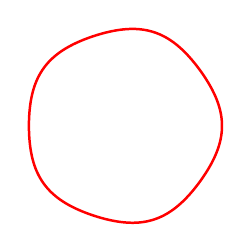
\begin{tikzpicture}[scale=0.45]

  \begin{axis}[
    hide axis,
    axis equal image,
    xmin = -1.42,
    xmax = 1.42,
    ymin = -1.42,
    ymax = 1.42,
    xtick = \empty,
    ytick = \empty,
    title style={align=left},
%    title={\Large $t = 3.17 \times 10^{-1}$ \\ \\ \Large $\nu = 0.99$}
  ]

\addplot[red,line width=2pt] coordinates{
(1.3864e+00,-4.3575e-10)
(1.3860e+00,2.7820e-02)
(1.3847e+00,5.6320e-02)
(1.3823e+00,8.6084e-02)
(1.3788e+00,1.1752e-01)
(1.3739e+00,1.5087e-01)
(1.3674e+00,1.8615e-01)
(1.3591e+00,2.2325e-01)
(1.3488e+00,2.6191e-01)
(1.3367e+00,3.0178e-01)
(1.3226e+00,3.4244e-01)
(1.3068e+00,3.8343e-01)
(1.2894e+00,4.2430e-01)
(1.2707e+00,4.6458e-01)
(1.2512e+00,5.0382e-01)
(1.2311e+00,5.4160e-01)
(1.2109e+00,5.7754e-01)
(1.1911e+00,6.1127e-01)
(1.1719e+00,6.4247e-01)
(1.1539e+00,6.7088e-01)
(1.1372e+00,6.9627e-01)
(1.1223e+00,7.1848e-01)
(1.1093e+00,7.3745e-01)
(1.0982e+00,7.5324e-01)
(1.0891e+00,7.6613e-01)
(1.0814e+00,7.7680e-01)
(1.0744e+00,7.8649e-01)
(1.0668e+00,7.9678e-01)
(1.0578e+00,8.0899e-01)
(1.0466e+00,8.2380e-01)
(1.0331e+00,8.4148e-01)
(1.0171e+00,8.6199e-01)
(9.9861e-01,8.8515e-01)
(9.7765e-01,9.1067e-01)
(9.5434e-01,9.3817e-01)
(9.2882e-01,9.6722e-01)
(9.0126e-01,9.9735e-01)
(8.7187e-01,1.0281e+00)
(8.4088e-01,1.0588e+00)
(8.0857e-01,1.0892e+00)
(7.7524e-01,1.1186e+00)
(7.4124e-01,1.1467e+00)
(7.0693e-01,1.1730e+00)
(6.7270e-01,1.1973e+00)
(6.3895e-01,1.2194e+00)
(6.0603e-01,1.2392e+00)
(5.7424e-01,1.2568e+00)
(5.4378e-01,1.2722e+00)
(5.1469e-01,1.2856e+00)
(4.8689e-01,1.2973e+00)
(4.6005e-01,1.3077e+00)
(4.3370e-01,1.3169e+00)
(4.0721e-01,1.3252e+00)
(3.7993e-01,1.3329e+00)
(3.5125e-01,1.3399e+00)
(3.2068e-01,1.3464e+00)
(2.8790e-01,1.3522e+00)
(2.5280e-01,1.3571e+00)
(2.1539e-01,1.3609e+00)
(1.7586e-01,1.3634e+00)
(1.3451e-01,1.3645e+00)
(9.1724e-02,1.3640e+00)
(4.7970e-02,1.3619e+00)
(3.7546e-03,1.3583e+00)
(-4.0394e-02,1.3532e+00)
(-8.3942e-02,1.3470e+00)
(-1.2636e-01,1.3397e+00)
(-1.6716e-01,1.3318e+00)
(-2.0585e-01,1.3234e+00)
(-2.4200e-01,1.3148e+00)
(-2.7522e-01,1.3064e+00)
(-3.0519e-01,1.2983e+00)
(-3.3165e-01,1.2908e+00)
(-3.5445e-01,1.2841e+00)
(-3.7359e-01,1.2783e+00)
(-3.8931e-01,1.2734e+00)
(-4.0225e-01,1.2693e+00)
(-4.1371e-01,1.2656e+00)
(-4.2554e-01,1.2617e+00)
(-4.3940e-01,1.2571e+00)
(-4.5627e-01,1.2513e+00)
(-4.7656e-01,1.2442e+00)
(-5.0033e-01,1.2356e+00)
(-5.2744e-01,1.2255e+00)
(-5.5761e-01,1.2137e+00)
(-5.9048e-01,1.2004e+00)
(-6.2561e-01,1.1854e+00)
(-6.6249e-01,1.1689e+00)
(-7.0061e-01,1.1507e+00)
(-7.3939e-01,1.1310e+00)
(-7.7827e-01,1.1099e+00)
(-8.1670e-01,1.0876e+00)
(-8.5415e-01,1.0641e+00)
(-8.9013e-01,1.0398e+00)
(-9.2424e-01,1.0148e+00)
(-9.5617e-01,9.8955e-01)
(-9.8569e-01,9.6433e-01)
(-1.0127e+00,9.3942e-01)
(-1.0373e+00,9.1507e-01)
(-1.0595e+00,8.9142e-01)
(-1.0796e+00,8.6848e-01)
(-1.0980e+00,8.4607e-01)
(-1.1151e+00,8.2386e-01)
(-1.1313e+00,8.0137e-01)
(-1.1471e+00,7.7803e-01)
(-1.1627e+00,7.5329e-01)
(-1.1783e+00,7.2664e-01)
(-1.1939e+00,6.9774e-01)
(-1.2095e+00,6.6637e-01)
(-1.2247e+00,6.3247e-01)
(-1.2395e+00,5.9612e-01)
(-1.2535e+00,5.5754e-01)
(-1.2664e+00,5.1703e-01)
(-1.2782e+00,4.7502e-01)
(-1.2887e+00,4.3199e-01)
(-1.2978e+00,3.8847e-01)
(-1.3056e+00,3.4504e-01)
(-1.3121e+00,3.0225e-01)
(-1.3173e+00,2.6068e-01)
(-1.3215e+00,2.2087e-01)
(-1.3247e+00,1.8334e-01)
(-1.3271e+00,1.4853e-01)
(-1.3288e+00,1.1687e-01)
(-1.3299e+00,8.8668e-02)
(-1.3307e+00,6.4158e-02)
(-1.3311e+00,4.3415e-02)
(-1.3314e+00,2.6286e-02)
(-1.3315e+00,1.2214e-02)
(-1.3315e+00,2.3306e-10)
(-1.3315e+00,-1.2214e-02)
(-1.3314e+00,-2.6286e-02)
(-1.3311e+00,-4.3415e-02)
(-1.3307e+00,-6.4158e-02)
(-1.3299e+00,-8.8668e-02)
(-1.3288e+00,-1.1687e-01)
(-1.3271e+00,-1.4853e-01)
(-1.3247e+00,-1.8334e-01)
(-1.3215e+00,-2.2087e-01)
(-1.3173e+00,-2.6068e-01)
(-1.3121e+00,-3.0225e-01)
(-1.3056e+00,-3.4504e-01)
(-1.2978e+00,-3.8847e-01)
(-1.2887e+00,-4.3199e-01)
(-1.2782e+00,-4.7502e-01)
(-1.2664e+00,-5.1703e-01)
(-1.2535e+00,-5.5754e-01)
(-1.2395e+00,-5.9612e-01)
(-1.2247e+00,-6.3247e-01)
(-1.2095e+00,-6.6637e-01)
(-1.1939e+00,-6.9774e-01)
(-1.1783e+00,-7.2664e-01)
(-1.1627e+00,-7.5329e-01)
(-1.1471e+00,-7.7803e-01)
(-1.1313e+00,-8.0137e-01)
(-1.1151e+00,-8.2386e-01)
(-1.0980e+00,-8.4607e-01)
(-1.0796e+00,-8.6848e-01)
(-1.0595e+00,-8.9142e-01)
(-1.0373e+00,-9.1507e-01)
(-1.0127e+00,-9.3942e-01)
(-9.8569e-01,-9.6433e-01)
(-9.5617e-01,-9.8955e-01)
(-9.2424e-01,-1.0148e+00)
(-8.9013e-01,-1.0398e+00)
(-8.5415e-01,-1.0641e+00)
(-8.1670e-01,-1.0876e+00)
(-7.7827e-01,-1.1099e+00)
(-7.3939e-01,-1.1310e+00)
(-7.0061e-01,-1.1507e+00)
(-6.6249e-01,-1.1689e+00)
(-6.2561e-01,-1.1854e+00)
(-5.9048e-01,-1.2004e+00)
(-5.5761e-01,-1.2137e+00)
(-5.2744e-01,-1.2255e+00)
(-5.0033e-01,-1.2356e+00)
(-4.7656e-01,-1.2442e+00)
(-4.5627e-01,-1.2513e+00)
(-4.3940e-01,-1.2571e+00)
(-4.2554e-01,-1.2617e+00)
(-4.1371e-01,-1.2656e+00)
(-4.0225e-01,-1.2693e+00)
(-3.8931e-01,-1.2734e+00)
(-3.7359e-01,-1.2783e+00)
(-3.5445e-01,-1.2841e+00)
(-3.3165e-01,-1.2908e+00)
(-3.0519e-01,-1.2983e+00)
(-2.7522e-01,-1.3064e+00)
(-2.4200e-01,-1.3148e+00)
(-2.0585e-01,-1.3234e+00)
(-1.6716e-01,-1.3318e+00)
(-1.2636e-01,-1.3397e+00)
(-8.3942e-02,-1.3470e+00)
(-4.0394e-02,-1.3532e+00)
(3.7546e-03,-1.3583e+00)
(4.7970e-02,-1.3619e+00)
(9.1724e-02,-1.3640e+00)
(1.3451e-01,-1.3645e+00)
(1.7586e-01,-1.3634e+00)
(2.1539e-01,-1.3609e+00)
(2.5280e-01,-1.3571e+00)
(2.8790e-01,-1.3522e+00)
(3.2068e-01,-1.3464e+00)
(3.5125e-01,-1.3399e+00)
(3.7993e-01,-1.3329e+00)
(4.0721e-01,-1.3252e+00)
(4.3370e-01,-1.3169e+00)
(4.6005e-01,-1.3077e+00)
(4.8689e-01,-1.2973e+00)
(5.1469e-01,-1.2856e+00)
(5.4378e-01,-1.2722e+00)
(5.7424e-01,-1.2568e+00)
(6.0603e-01,-1.2392e+00)
(6.3895e-01,-1.2194e+00)
(6.7270e-01,-1.1973e+00)
(7.0693e-01,-1.1730e+00)
(7.4124e-01,-1.1467e+00)
(7.7524e-01,-1.1186e+00)
(8.0857e-01,-1.0892e+00)
(8.4088e-01,-1.0588e+00)
(8.7187e-01,-1.0281e+00)
(9.0126e-01,-9.9735e-01)
(9.2882e-01,-9.6722e-01)
(9.5434e-01,-9.3817e-01)
(9.7765e-01,-9.1067e-01)
(9.9861e-01,-8.8515e-01)
(1.0171e+00,-8.6199e-01)
(1.0331e+00,-8.4148e-01)
(1.0466e+00,-8.2380e-01)
(1.0578e+00,-8.0899e-01)
(1.0668e+00,-7.9678e-01)
(1.0744e+00,-7.8649e-01)
(1.0814e+00,-7.7680e-01)
(1.0891e+00,-7.6613e-01)
(1.0982e+00,-7.5324e-01)
(1.1093e+00,-7.3745e-01)
(1.1223e+00,-7.1848e-01)
(1.1372e+00,-6.9627e-01)
(1.1539e+00,-6.7088e-01)
(1.1719e+00,-6.4247e-01)
(1.1911e+00,-6.1127e-01)
(1.2109e+00,-5.7754e-01)
(1.2311e+00,-5.4160e-01)
(1.2512e+00,-5.0382e-01)
(1.2707e+00,-4.6458e-01)
(1.2894e+00,-4.2430e-01)
(1.3068e+00,-3.8343e-01)
(1.3226e+00,-3.4244e-01)
(1.3367e+00,-3.0178e-01)
(1.3488e+00,-2.6191e-01)
(1.3591e+00,-2.2325e-01)
(1.3674e+00,-1.8615e-01)
(1.3739e+00,-1.5087e-01)
(1.3788e+00,-1.1752e-01)
(1.3823e+00,-8.6084e-02)
(1.3847e+00,-5.6320e-02)
(1.3860e+00,-2.7820e-02)
(1.3864e+00,-4.3575e-10)
};



\end{axis}

\end{tikzpicture}

%    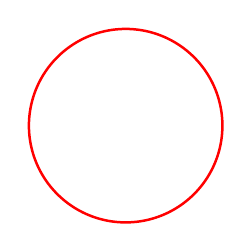
\begin{tikzpicture}[scale=0.45]

  \begin{axis}[
    hide axis,
    axis equal image,
    xmin = -1.42,
    xmax = 1.42,
    ymin = -1.42,
    ymax = 1.42,
    xtick = \empty,
    ytick = \empty,
    title style={align=left},
%    title={\Large $t = 1.00 \times 10^{0}$ \\ \\ \Large $\nu = 1.00$}
  ]

\addplot[red,line width=2pt] coordinates{
(1.3619e+00,-2.0922e-10)
(1.3616e+00,2.7822e-02)
(1.3608e+00,5.6341e-02)
(1.3592e+00,8.6156e-02)
(1.3568e+00,1.1771e-01)
(1.3535e+00,1.5125e-01)
(1.3490e+00,1.8685e-01)
(1.3433e+00,2.2444e-01)
(1.3361e+00,2.6377e-01)
(1.3274e+00,3.0454e-01)
(1.3172e+00,3.4632e-01)
(1.3053e+00,3.8864e-01)
(1.2919e+00,4.3100e-01)
(1.2772e+00,4.7288e-01)
(1.2613e+00,5.1374e-01)
(1.2446e+00,5.5311e-01)
(1.2273e+00,5.9051e-01)
(1.2098e+00,6.2553e-01)
(1.1925e+00,6.5782e-01)
(1.1759e+00,6.8709e-01)
(1.1603e+00,7.1312e-01)
(1.1461e+00,7.3578e-01)
(1.1335e+00,7.5504e-01)
(1.1227e+00,7.7100e-01)
(1.1137e+00,7.8398e-01)
(1.1060e+00,7.9469e-01)
(1.0990e+00,8.0438e-01)
(1.0914e+00,8.1464e-01)
(1.0823e+00,8.2676e-01)
(1.0709e+00,8.4142e-01)
(1.0570e+00,8.5881e-01)
(1.0404e+00,8.7884e-01)
(1.0210e+00,9.0128e-01)
(9.9889e-01,9.2577e-01)
(9.7404e-01,9.5189e-01)
(9.4662e-01,9.7916e-01)
(9.1684e-01,1.0071e+00)
(8.8497e-01,1.0352e+00)
(8.5132e-01,1.0631e+00)
(8.1628e-01,1.0902e+00)
(7.8026e-01,1.1163e+00)
(7.4372e-01,1.1409e+00)
(7.0712e-01,1.1640e+00)
(6.7091e-01,1.1852e+00)
(6.3551e-01,1.2046e+00)
(6.0127e-01,1.2220e+00)
(5.6847e-01,1.2376e+00)
(5.3727e-01,1.2515e+00)
(5.0769e-01,1.2638e+00)
(4.7956e-01,1.2747e+00)
(4.5254e-01,1.2845e+00)
(4.2613e-01,1.2935e+00)
(3.9967e-01,1.3020e+00)
(3.7249e-01,1.3100e+00)
(3.4398e-01,1.3178e+00)
(3.1365e-01,1.3253e+00)
(2.8118e-01,1.3326e+00)
(2.4640e-01,1.3395e+00)
(2.0933e-01,1.3457e+00)
(1.7011e-01,1.3513e+00)
(1.2899e-01,1.3558e+00)
(8.6333e-02,1.3592e+00)
(4.2577e-02,1.3613e+00)
(-1.7828e-03,1.3619e+00)
(-4.6212e-02,1.3611e+00)
(-9.0152e-02,1.3589e+00)
(-1.3305e-01,1.3554e+00)
(-1.7434e-01,1.3507e+00)
(-2.1353e-01,1.3451e+00)
(-2.5014e-01,1.3388e+00)
(-2.8375e-01,1.3320e+00)
(-3.1403e-01,1.3252e+00)
(-3.4072e-01,1.3186e+00)
(-3.6368e-01,1.3125e+00)
(-3.8292e-01,1.3070e+00)
(-3.9868e-01,1.3023e+00)
(-4.1165e-01,1.2982e+00)
(-4.2312e-01,1.2945e+00)
(-4.3494e-01,1.2906e+00)
(-4.4876e-01,1.2859e+00)
(-4.6555e-01,1.2799e+00)
(-4.8570e-01,1.2724e+00)
(-5.0922e-01,1.2631e+00)
(-5.3595e-01,1.2520e+00)
(-5.6556e-01,1.2389e+00)
(-5.9763e-01,1.2238e+00)
(-6.3170e-01,1.2066e+00)
(-6.6725e-01,1.1873e+00)
(-7.0372e-01,1.1660e+00)
(-7.4059e-01,1.1430e+00)
(-7.7731e-01,1.1183e+00)
(-8.1341e-01,1.0923e+00)
(-8.4843e-01,1.0654e+00)
(-8.8198e-01,1.0378e+00)
(-9.1376e-01,1.0099e+00)
(-9.4353e-01,9.8214e-01)
(-9.7114e-01,9.5484e-01)
(-9.9655e-01,9.2829e-01)
(-1.0198e+00,9.0270e-01)
(-1.0410e+00,8.7815e-01)
(-1.0604e+00,8.5460e-01)
(-1.0784e+00,8.3183e-01)
(-1.0953e+00,8.0946e-01)
(-1.1115e+00,7.8699e-01)
(-1.1276e+00,7.6384e-01)
(-1.1437e+00,7.3944e-01)
(-1.1602e+00,7.1331e-01)
(-1.1771e+00,6.8512e-01)
(-1.1943e+00,6.5464e-01)
(-1.2117e+00,6.2179e-01)
(-1.2291e+00,5.8664e-01)
(-1.2462e+00,5.4934e-01)
(-1.2628e+00,5.1015e-01)
(-1.2785e+00,4.6944e-01)
(-1.2931e+00,4.2762e-01)
(-1.3063e+00,3.8518e-01)
(-1.3181e+00,3.4266e-01)
(-1.3283e+00,3.0061e-01)
(-1.3370e+00,2.5961e-01)
(-1.3440e+00,2.2021e-01)
(-1.3496e+00,1.8295e-01)
(-1.3538e+00,1.4833e-01)
(-1.3569e+00,1.1677e-01)
(-1.3590e+00,8.8624e-02)
(-1.3604e+00,6.4142e-02)
(-1.3612e+00,4.3410e-02)
(-1.3617e+00,2.6284e-02)
(-1.3619e+00,1.2214e-02)
(-1.3619e+00,2.2277e-10)
(-1.3619e+00,-1.2214e-02)
(-1.3617e+00,-2.6284e-02)
(-1.3612e+00,-4.3410e-02)
(-1.3604e+00,-6.4142e-02)
(-1.3590e+00,-8.8624e-02)
(-1.3569e+00,-1.1677e-01)
(-1.3538e+00,-1.4833e-01)
(-1.3496e+00,-1.8295e-01)
(-1.3440e+00,-2.2021e-01)
(-1.3370e+00,-2.5961e-01)
(-1.3283e+00,-3.0061e-01)
(-1.3181e+00,-3.4266e-01)
(-1.3063e+00,-3.8518e-01)
(-1.2931e+00,-4.2762e-01)
(-1.2785e+00,-4.6944e-01)
(-1.2628e+00,-5.1015e-01)
(-1.2462e+00,-5.4934e-01)
(-1.2291e+00,-5.8664e-01)
(-1.2117e+00,-6.2179e-01)
(-1.1943e+00,-6.5464e-01)
(-1.1771e+00,-6.8512e-01)
(-1.1602e+00,-7.1331e-01)
(-1.1437e+00,-7.3944e-01)
(-1.1276e+00,-7.6384e-01)
(-1.1115e+00,-7.8699e-01)
(-1.0953e+00,-8.0946e-01)
(-1.0784e+00,-8.3183e-01)
(-1.0604e+00,-8.5460e-01)
(-1.0410e+00,-8.7815e-01)
(-1.0198e+00,-9.0270e-01)
(-9.9655e-01,-9.2829e-01)
(-9.7114e-01,-9.5484e-01)
(-9.4353e-01,-9.8214e-01)
(-9.1376e-01,-1.0099e+00)
(-8.8198e-01,-1.0378e+00)
(-8.4843e-01,-1.0654e+00)
(-8.1341e-01,-1.0923e+00)
(-7.7731e-01,-1.1183e+00)
(-7.4059e-01,-1.1430e+00)
(-7.0372e-01,-1.1660e+00)
(-6.6725e-01,-1.1873e+00)
(-6.3170e-01,-1.2066e+00)
(-5.9763e-01,-1.2238e+00)
(-5.6556e-01,-1.2389e+00)
(-5.3595e-01,-1.2520e+00)
(-5.0922e-01,-1.2631e+00)
(-4.8570e-01,-1.2724e+00)
(-4.6555e-01,-1.2799e+00)
(-4.4876e-01,-1.2859e+00)
(-4.3494e-01,-1.2906e+00)
(-4.2312e-01,-1.2945e+00)
(-4.1165e-01,-1.2982e+00)
(-3.9868e-01,-1.3023e+00)
(-3.8292e-01,-1.3070e+00)
(-3.6368e-01,-1.3125e+00)
(-3.4072e-01,-1.3186e+00)
(-3.1403e-01,-1.3252e+00)
(-2.8375e-01,-1.3320e+00)
(-2.5014e-01,-1.3388e+00)
(-2.1353e-01,-1.3451e+00)
(-1.7434e-01,-1.3507e+00)
(-1.3305e-01,-1.3554e+00)
(-9.0152e-02,-1.3589e+00)
(-4.6212e-02,-1.3611e+00)
(-1.7828e-03,-1.3619e+00)
(4.2577e-02,-1.3613e+00)
(8.6333e-02,-1.3592e+00)
(1.2899e-01,-1.3558e+00)
(1.7011e-01,-1.3513e+00)
(2.0933e-01,-1.3457e+00)
(2.4640e-01,-1.3395e+00)
(2.8118e-01,-1.3326e+00)
(3.1365e-01,-1.3253e+00)
(3.4398e-01,-1.3178e+00)
(3.7249e-01,-1.3100e+00)
(3.9967e-01,-1.3020e+00)
(4.2613e-01,-1.2935e+00)
(4.5254e-01,-1.2845e+00)
(4.7956e-01,-1.2747e+00)
(5.0769e-01,-1.2638e+00)
(5.3727e-01,-1.2515e+00)
(5.6847e-01,-1.2376e+00)
(6.0127e-01,-1.2220e+00)
(6.3551e-01,-1.2046e+00)
(6.7091e-01,-1.1852e+00)
(7.0712e-01,-1.1640e+00)
(7.4372e-01,-1.1409e+00)
(7.8026e-01,-1.1163e+00)
(8.1628e-01,-1.0902e+00)
(8.5132e-01,-1.0631e+00)
(8.8497e-01,-1.0352e+00)
(9.1684e-01,-1.0071e+00)
(9.4662e-01,-9.7916e-01)
(9.7404e-01,-9.5189e-01)
(9.9889e-01,-9.2577e-01)
(1.0210e+00,-9.0128e-01)
(1.0404e+00,-8.7884e-01)
(1.0570e+00,-8.5881e-01)
(1.0709e+00,-8.4142e-01)
(1.0823e+00,-8.2676e-01)
(1.0914e+00,-8.1464e-01)
(1.0990e+00,-8.0438e-01)
(1.1060e+00,-7.9469e-01)
(1.1137e+00,-7.8398e-01)
(1.1227e+00,-7.7100e-01)
(1.1335e+00,-7.5504e-01)
(1.1461e+00,-7.3578e-01)
(1.1603e+00,-7.1312e-01)
(1.1759e+00,-6.8709e-01)
(1.1925e+00,-6.5782e-01)
(1.2098e+00,-6.2553e-01)
(1.2273e+00,-5.9051e-01)
(1.2446e+00,-5.5311e-01)
(1.2613e+00,-5.1374e-01)
(1.2772e+00,-4.7288e-01)
(1.2919e+00,-4.3100e-01)
(1.3053e+00,-3.8864e-01)
(1.3172e+00,-3.4632e-01)
(1.3274e+00,-3.0454e-01)
(1.3361e+00,-2.6377e-01)
(1.3433e+00,-2.2444e-01)
(1.3490e+00,-1.8685e-01)
(1.3535e+00,-1.5125e-01)
(1.3568e+00,-1.1771e-01)
(1.3592e+00,-8.6156e-02)
(1.3608e+00,-5.6341e-02)
(1.3616e+00,-2.7822e-02)
(1.3619e+00,-2.0922e-10)
};



\end{axis}

\end{tikzpicture}

%%    \fi
%  \end{minipage}
%  \hfill
%  \begin{minipage}{0.4\textwidth}
%%  \ifTikz
%  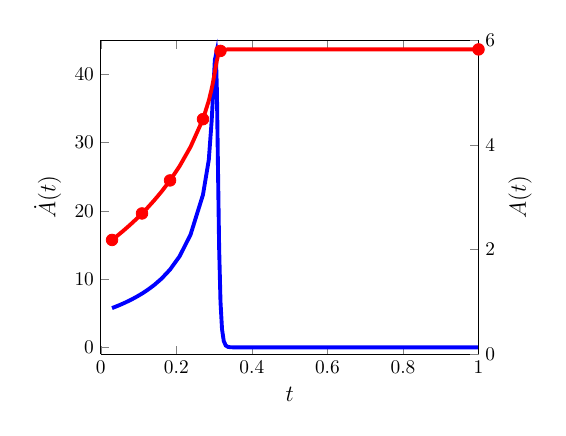
\begin{tikzpicture}[scale=0.7]

  \begin{axis}[
    label = area,
    axis y line*=left,
    xmin = 0,
    xmax = 1,
    ymin = -1,
    ymax = 45,
%    xtick = \empty,
%    ytick = \empty,
    xlabel = {\large $t$},
    ylabel = {\large $\dot{A}(t)$},
    ylabel near ticks,
    clip = false,
  ]

\addplot[blue, line width=2pt] coordinates{
(2.9870e-02,5.7561e+00)
(3.4004e-02,5.8445e+00)
(3.8711e-02,5.9473e+00)
(4.4069e-02,6.0675e+00)
(5.0169e-02,6.2087e+00)
(5.7113e-02,6.3756e+00)
(6.5018e-02,6.5740e+00)
(7.4018e-02,6.8114e+00)
(8.4263e-02,7.0984e+00)
(9.5927e-02,7.4491e+00)
(1.0920e-01,7.8837e+00)
(1.2432e-01,8.4323e+00)
(1.4153e-01,9.1412e+00)
(1.6112e-01,1.0086e+01)
(1.8342e-01,1.1403e+01)
(2.0881e-01,1.3355e+01)
(2.3771e-01,1.6528e+01)
(2.7062e-01,2.2375e+01)
(2.8600e-01,2.7491e+01)
(2.9355e-01,3.3172e+01)
(2.9843e-01,3.8204e+01)
(3.0194e-01,4.2097e+01)
(3.0477e-01,4.2847e+01)
(3.0746e-01,3.7637e+01)
(3.1022e-01,2.6545e+01)
(3.1336e-01,1.4603e+01)
(3.1693e-01,6.7105e+00)
(3.2099e-01,2.6631e+00)
(3.2562e-01,9.1879e-01)
(3.3089e-01,2.7242e-01)
(3.3689e-01,6.8267e-02)
(3.4372e-01,1.4117e-02)
(3.5149e-01,2.3475e-03)
(3.6034e-01,3.0278e-04)
(3.7042e-01,2.9334e-05)
(3.8189e-01,1.8397e-06)
(3.9495e-01,2.9182e-08)
(4.0981e-01,-1.1297e-07)
(4.2673e-01,-8.9110e-08)
(4.4600e-01,-1.0247e-07)
(4.6793e-01,-9.5801e-08)
(4.9290e-01,-9.8909e-08)
(5.2132e-01,-9.7487e-08)
(5.5368e-01,-9.8115e-08)
(5.9052e-01,-9.7979e-08)
(6.3245e-01,-9.8076e-08)
(6.8019e-01,-9.8003e-08)
(7.3454e-01,-9.7982e-08)
(7.9642e-01,-9.8078e-08)
(8.6685e-01,-9.7981e-08)
(9.4704e-01,-9.8083e-08)
(1.0000e+00,-9.7890e-08)
};

%\node at (axis cs:0,45) [anchor=south east] {(a)};

\end{axis}

  \begin{axis}[
    axis y line*=right,
    axis x line=none,
    xmin = 0,
    xmax = 1,
    ymin = 0,
    ymax = 6,
%    xtick = \empty,
%    ytick = \empty,
    ylabel = {\large $A(t)$},
    ylabel near ticks,
  ]


\addplot[red,line width=2pt] coordinates{
(2.9870e-02,2.1842e+00)
(3.4004e-02,2.2076e+00)
(3.8711e-02,2.2346e+00)
(4.4069e-02,2.2658e+00)
(5.0169e-02,2.3019e+00)
(5.7113e-02,2.3438e+00)
(6.5018e-02,2.3927e+00)
(7.4018e-02,2.4498e+00)
(8.4263e-02,2.5170e+00)
(9.5927e-02,2.5963e+00)
(1.0920e-01,2.6907e+00)
(1.2432e-01,2.8039e+00)
(1.4153e-01,2.9413e+00)
(1.6112e-01,3.1103e+00)
(1.8342e-01,3.3225e+00)
(2.0881e-01,3.5962e+00)
(2.3771e-01,3.9645e+00)
(2.7062e-01,4.4934e+00)
(2.8600e-01,4.8471e+00)
(2.9355e-01,5.0730e+00)
(2.9843e-01,5.2478e+00)
(3.0194e-01,5.3903e+00)
(3.0477e-01,5.5117e+00)
(3.0746e-01,5.6188e+00)
(3.1022e-01,5.7036e+00)
(3.1336e-01,5.7637e+00)
(3.1693e-01,5.7985e+00)
(3.2099e-01,5.8158e+00)
(3.2562e-01,5.8232e+00)
(3.3089e-01,5.8260e+00)
(3.3689e-01,5.8269e+00)
(3.4372e-01,5.8271e+00)
(3.5149e-01,5.8272e+00)
(3.6034e-01,5.8272e+00)
(3.7042e-01,5.8272e+00)
(3.8189e-01,5.8272e+00)
(3.9495e-01,5.8272e+00)
(4.0981e-01,5.8272e+00)
(4.2673e-01,5.8272e+00)
(4.4600e-01,5.8272e+00)
(4.6793e-01,5.8272e+00)
(4.9290e-01,5.8272e+00)
(5.2132e-01,5.8272e+00)
(5.5368e-01,5.8272e+00)
(5.9052e-01,5.8272e+00)
(6.3245e-01,5.8272e+00)
(6.8019e-01,5.8272e+00)
(7.3454e-01,5.8272e+00)
(7.9642e-01,5.8272e+00)
(8.6685e-01,5.8272e+00)
(9.4704e-01,5.8272e+00)
(1.0000e+00,5.8272e+00)
};

\addplot[red,only marks,mark size=3pt] coordinates{
(2.9870e-02,2.1842e+00)
(1.0920e-01,2.6907e+00)
(1.8342e-01,3.3225e+00)
(2.7062e-01,4.4934e+00)
(3.1693e-01,5.7985e+00)
(1.0000e+00,5.8272e+00)
};



\end{axis}



\end{tikzpicture}

%%  \fi
%  \end{minipage}
%%  \caption{\label{fig:starShape} A initially star-shaped semi-permeable
%%  vesicle in a shear quiescent flow with $\beta=1$. Note that the time
%%  steps are not equispaced. The area (red) and its derivative (blue) of
%%  an initially star-shaped vesicle as a function of time. The dots
%%  correspond to the time steps shown in six time steps
%%  show on the left.}
%\end{figure}
%
%\begin{table}[htp]
%  \centering
%  \begin{tabular}{|C{1cm}|*{6}{C{2cm}}|}
%    \hline
%    $\beta$ & $10^{0}$ & $10^{-1}$ & $10^{-2}$ & 
%             $10^{-3}$ & $10^{-4}$ & $10^{-5}$ \\
%    $t_\mathrm{SS}$ & $6.45 \times 10^{0}$ & $2.00 \times 10^{1}$ & 
%                      $9.61 \times 10^{1}$ & $8.36 \times 10^{2}$ & 
%                      $8.15 \times 10^{3}$ & $8.03 \times 10^{4}$ \\
%    ratio & --- & 3.10 & 4.81 & 8.71 & 9.74 & 9.85 \\
%    \hline
%  \end{tabular}
%  \caption{\label{tbl:ellipseRelaxTime} The time, $t_{\mathrm{SS}}$, for
%  a semi-permeable vesicle to reach steady state.}
%\end{table}
%
%\begin{table}[htp]
%  \centering
%  \begin{tabular}{|C{1cm}|*{6}{C{2cm}}|}
%    \hline
%    $\beta$ & $10^{0}$ & $10^{-1}$ & $10^{-2}$ & 
%             $10^{-3}$ & $10^{-4}$ & $10^{-5}$ \\
%    $t_\mathrm{SP}$ & $2.17 \times 10^{-2}$ & $1.25 \times 10^{-1}$ & 
%                      $1.59 \times 10^{0}$ & $2.19 \times 10^{1}$ & 
%                      $2.14 \times 10^{2}$ & $2.20 \times 10^{3}$ \\
%    ratio & --- & 5.76 & 12.72 & 13.77 & 9.77 & 10.14 \\
%    \hline
%  \end{tabular}
%  \caption{\label{tbl:ellipseBLTime} The time, $t_\mathrm{SP}$, for a
%  semi-permeable vesicle to begin inflating.}
%\end{table}
%
%%\begin{figure}[htp]
%%\begin{minipage}{0.40\textwidth}
%%\ifTikz
%%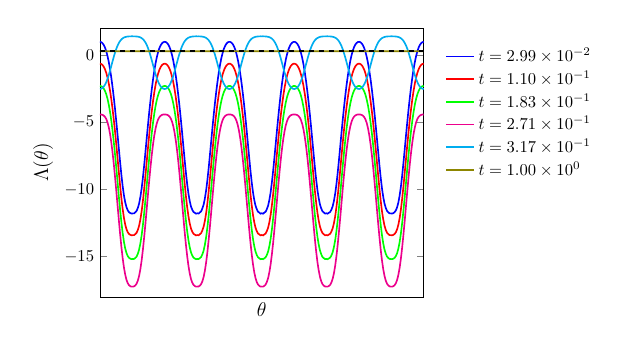
\begin{tikzpicture}[scale=0.6]

  \begin{axis}[
    xmin = 0,
    xmax = 6.2832,
    ymin = -18,
    ymax = 2,
    xtick = \empty,
    ylabel near ticks,
    xlabel = {\large $\theta$},
    ylabel = {\large $\Lambda(\theta)$},
    clip = false,
    legend entries = {$t=2.99 \times 10^{-2}$,
    $t = 1.10 \times 10^{-1}$,
    $t = 1.83 \times 10^{-1}$,
    $t = 2.71 \times 10^{-1}$,
    $t = 3.17 \times 10^{-1}$,
    $t = 1.00 \times 10^{0}$},
    legend cell align=left,
    legend style={draw=none},
    legend style={at={(1.05,0.95)},anchor=north west}
  ]


\addplot[blue,line width=1pt] coordinates{
(0.0000e+00,9.7332e-01)
(2.4544e-02,9.5053e-01)
(4.9087e-02,8.7407e-01)
(7.3631e-02,7.4345e-01)
(9.8175e-02,5.4519e-01)
(1.2272e-01,2.7392e-01)
(1.4726e-01,-8.1963e-02)
(1.7181e-01,-5.2587e-01)
(1.9635e-01,-1.0619e+00)
(2.2089e-01,-1.6879e+00)
(2.4544e-01,-2.4009e+00)
(2.6998e-01,-3.1957e+00)
(2.9452e-01,-4.0665e+00)
(3.1907e-01,-5.0048e+00)
(3.4361e-01,-5.9949e+00)
(3.6816e-01,-7.0104e+00)
(3.9270e-01,-8.0105e+00)
(4.1724e-01,-8.9464e+00)
(4.4179e-01,-9.7689e+00)
(4.6633e-01,-1.0445e+01)
(4.9087e-01,-1.0959e+01)
(5.1542e-01,-1.1322e+01)
(5.3996e-01,-1.1556e+01)
(5.6450e-01,-1.1694e+01)
(5.8905e-01,-1.1761e+01)
(6.1359e-01,-1.1796e+01)
(6.3814e-01,-1.1785e+01)
(6.6268e-01,-1.1781e+01)
(6.8722e-01,-1.1703e+01)
(7.1177e-01,-1.1598e+01)
(7.3631e-01,-1.1373e+01)
(7.6085e-01,-1.1048e+01)
(7.8540e-01,-1.0556e+01)
(8.0994e-01,-9.9198e+00)
(8.3449e-01,-9.1187e+00)
(8.5903e-01,-8.2065e+00)
(8.8357e-01,-7.2117e+00)
(9.0812e-01,-6.1982e+00)
(9.3266e-01,-5.1986e+00)
(9.5720e-01,-4.2496e+00)
(9.8175e-01,-3.3638e+00)
(1.0063e+00,-2.5535e+00)
(1.0308e+00,-1.8239e+00)
(1.0554e+00,-1.1796e+00)
(1.0799e+00,-6.2629e-01)
(1.1045e+00,-1.6283e-01)
(1.1290e+00,2.0889e-01)
(1.1536e+00,4.9796e-01)
(1.1781e+00,7.0867e-01)
(1.2026e+00,8.5323e-01)
(1.2272e+00,9.3921e-01)
(1.2517e+00,9.7257e-01)
(1.2763e+00,9.5943e-01)
(1.3008e+00,8.9299e-01)
(1.3254e+00,7.7536e-01)
(1.3499e+00,5.8960e-01)
(1.3744e+00,3.3549e-01)
(1.3990e+00,-4.6191e-03)
(1.4235e+00,-4.2912e-01)
(1.4481e+00,-9.4790e-01)
(1.4726e+00,-1.5553e+00)
(1.4972e+00,-2.2517e+00)
(1.5217e+00,-3.0306e+00)
(1.5463e+00,-3.8863e+00)
(1.5708e+00,-4.8130e+00)
(1.5953e+00,-5.7928e+00)
(1.6199e+00,-6.8084e+00)
(1.6444e+00,-7.8122e+00)
(1.6690e+00,-8.7692e+00)
(1.6935e+00,-9.6124e+00)
(1.7181e+00,-1.0326e+01)
(1.7426e+00,-1.0865e+01)
(1.7671e+00,-1.1267e+01)
(1.7917e+00,-1.1512e+01)
(1.8162e+00,-1.1681e+01)
(1.8408e+00,-1.1741e+01)
(1.8653e+00,-1.1804e+01)
(1.8899e+00,-1.1776e+01)
(1.9144e+00,-1.1797e+01)
(1.9390e+00,-1.1712e+01)
(1.9635e+00,-1.1634e+01)
(1.9880e+00,-1.1420e+01)
(2.0126e+00,-1.1130e+01)
(2.0371e+00,-1.0663e+01)
(2.0617e+00,-1.0064e+01)
(2.0862e+00,-9.2869e+00)
(2.1108e+00,-8.3989e+00)
(2.1353e+00,-7.4123e+00)
(2.1598e+00,-6.4020e+00)
(2.1844e+00,-5.3945e+00)
(2.2089e+00,-4.4353e+00)
(2.2335e+00,-3.5349e+00)
(2.2580e+00,-2.7094e+00)
(2.2826e+00,-1.9632e+00)
(2.3071e+00,-1.3010e+00)
(2.3317e+00,-7.3017e-01)
(2.3562e+00,-2.4753e-01)
(2.3807e+00,1.4070e-01)
(2.4053e+00,4.4747e-01)
(2.4298e+00,6.7129e-01)
(2.4544e+00,8.3009e-01)
(2.4789e+00,9.2567e-01)
(2.5035e+00,9.7019e-01)
(2.5280e+00,9.6592e-01)
(2.5525e+00,9.1019e-01)
(2.5771e+00,8.0422e-01)
(2.6016e+00,6.3158e-01)
(2.6262e+00,3.9337e-01)
(2.6507e+00,6.9535e-02)
(2.6753e+00,-3.3629e-01)
(2.6998e+00,-8.3736e-01)
(2.7243e+00,-1.4263e+00)
(2.7489e+00,-2.1058e+00)
(2.7734e+00,-2.8684e+00)
(2.7980e+00,-3.7090e+00)
(2.8225e+00,-4.6232e+00)
(2.8471e+00,-5.5926e+00)
(2.8716e+00,-6.6055e+00)
(2.8962e+00,-7.6126e+00)
(2.9207e+00,-8.5866e+00)
(2.9452e+00,-9.4515e+00)
(2.9698e+00,-1.0199e+01)
(2.9943e+00,-1.0766e+01)
(3.0189e+00,-1.1203e+01)
(3.0434e+00,-1.1466e+01)
(3.0680e+00,-1.1661e+01)
(3.0925e+00,-1.1724e+01)
(3.1170e+00,-1.1805e+01)
(3.1416e+00,-1.1772e+01)
(3.1661e+00,-1.1805e+01)
(3.1907e+00,-1.1724e+01)
(3.2152e+00,-1.1661e+01)
(3.2398e+00,-1.1466e+01)
(3.2643e+00,-1.1203e+01)
(3.2889e+00,-1.0766e+01)
(3.3134e+00,-1.0199e+01)
(3.3379e+00,-9.4515e+00)
(3.3625e+00,-8.5866e+00)
(3.3870e+00,-7.6126e+00)
(3.4116e+00,-6.6055e+00)
(3.4361e+00,-5.5926e+00)
(3.4607e+00,-4.6232e+00)
(3.4852e+00,-3.7090e+00)
(3.5097e+00,-2.8684e+00)
(3.5343e+00,-2.1058e+00)
(3.5588e+00,-1.4263e+00)
(3.5834e+00,-8.3736e-01)
(3.6079e+00,-3.3629e-01)
(3.6325e+00,6.9535e-02)
(3.6570e+00,3.9337e-01)
(3.6816e+00,6.3158e-01)
(3.7061e+00,8.0422e-01)
(3.7306e+00,9.1019e-01)
(3.7552e+00,9.6592e-01)
(3.7797e+00,9.7019e-01)
(3.8043e+00,9.2567e-01)
(3.8288e+00,8.3009e-01)
(3.8534e+00,6.7129e-01)
(3.8779e+00,4.4747e-01)
(3.9024e+00,1.4070e-01)
(3.9270e+00,-2.4753e-01)
(3.9515e+00,-7.3017e-01)
(3.9761e+00,-1.3010e+00)
(4.0006e+00,-1.9632e+00)
(4.0252e+00,-2.7094e+00)
(4.0497e+00,-3.5349e+00)
(4.0743e+00,-4.4353e+00)
(4.0988e+00,-5.3945e+00)
(4.1233e+00,-6.4020e+00)
(4.1479e+00,-7.4123e+00)
(4.1724e+00,-8.3989e+00)
(4.1970e+00,-9.2869e+00)
(4.2215e+00,-1.0064e+01)
(4.2461e+00,-1.0663e+01)
(4.2706e+00,-1.1130e+01)
(4.2951e+00,-1.1420e+01)
(4.3197e+00,-1.1634e+01)
(4.3442e+00,-1.1712e+01)
(4.3688e+00,-1.1797e+01)
(4.3933e+00,-1.1776e+01)
(4.4179e+00,-1.1804e+01)
(4.4424e+00,-1.1741e+01)
(4.4670e+00,-1.1681e+01)
(4.4915e+00,-1.1512e+01)
(4.5160e+00,-1.1267e+01)
(4.5406e+00,-1.0865e+01)
(4.5651e+00,-1.0326e+01)
(4.5897e+00,-9.6124e+00)
(4.6142e+00,-8.7692e+00)
(4.6388e+00,-7.8122e+00)
(4.6633e+00,-6.8084e+00)
(4.6878e+00,-5.7928e+00)
(4.7124e+00,-4.8130e+00)
(4.7369e+00,-3.8863e+00)
(4.7615e+00,-3.0306e+00)
(4.7860e+00,-2.2517e+00)
(4.8106e+00,-1.5553e+00)
(4.8351e+00,-9.4790e-01)
(4.8597e+00,-4.2912e-01)
(4.8842e+00,-4.6191e-03)
(4.9087e+00,3.3549e-01)
(4.9333e+00,5.8960e-01)
(4.9578e+00,7.7536e-01)
(4.9824e+00,8.9299e-01)
(5.0069e+00,9.5943e-01)
(5.0315e+00,9.7257e-01)
(5.0560e+00,9.3921e-01)
(5.0805e+00,8.5323e-01)
(5.1051e+00,7.0867e-01)
(5.1296e+00,4.9796e-01)
(5.1542e+00,2.0889e-01)
(5.1787e+00,-1.6283e-01)
(5.2033e+00,-6.2629e-01)
(5.2278e+00,-1.1796e+00)
(5.2524e+00,-1.8239e+00)
(5.2769e+00,-2.5535e+00)
(5.3014e+00,-3.3638e+00)
(5.3260e+00,-4.2496e+00)
(5.3505e+00,-5.1986e+00)
(5.3751e+00,-6.1982e+00)
(5.3996e+00,-7.2117e+00)
(5.4242e+00,-8.2065e+00)
(5.4487e+00,-9.1187e+00)
(5.4732e+00,-9.9198e+00)
(5.4978e+00,-1.0556e+01)
(5.5223e+00,-1.1048e+01)
(5.5469e+00,-1.1373e+01)
(5.5714e+00,-1.1598e+01)
(5.5960e+00,-1.1703e+01)
(5.6205e+00,-1.1781e+01)
(5.6450e+00,-1.1785e+01)
(5.6696e+00,-1.1796e+01)
(5.6941e+00,-1.1761e+01)
(5.7187e+00,-1.1694e+01)
(5.7432e+00,-1.1556e+01)
(5.7678e+00,-1.1322e+01)
(5.7923e+00,-1.0959e+01)
(5.8169e+00,-1.0445e+01)
(5.8414e+00,-9.7689e+00)
(5.8659e+00,-8.9464e+00)
(5.8905e+00,-8.0105e+00)
(5.9150e+00,-7.0104e+00)
(5.9396e+00,-5.9949e+00)
(5.9641e+00,-5.0048e+00)
(5.9887e+00,-4.0665e+00)
(6.0132e+00,-3.1957e+00)
(6.0377e+00,-2.4009e+00)
(6.0623e+00,-1.6879e+00)
(6.0868e+00,-1.0619e+00)
(6.1114e+00,-5.2587e-01)
(6.1359e+00,-8.1963e-02)
(6.1605e+00,2.7392e-01)
(6.1850e+00,5.4519e-01)
(6.2096e+00,7.4345e-01)
(6.2341e+00,8.7407e-01)
(6.2586e+00,9.5053e-01)
(6.2832e+00,9.7332e-01)
};

\addplot[red,line width=1pt] coordinates{
(0.0000e+00,-6.5079e-01)
(2.4544e-02,-6.7293e-01)
(4.9087e-02,-7.4659e-01)
(7.3631e-02,-8.7322e-01)
(9.8175e-02,-1.0660e+00)
(1.2272e-01,-1.3316e+00)
(1.4726e-01,-1.6823e+00)
(1.7181e-01,-2.1235e+00)
(1.9635e-01,-2.6612e+00)
(2.2089e-01,-3.2953e+00)
(2.4544e-01,-4.0249e+00)
(2.6998e-01,-4.8447e+00)
(2.9452e-01,-5.7468e+00)
(3.1907e-01,-6.7172e+00)
(3.4361e-01,-7.7329e+00)
(3.6816e-01,-8.7606e+00)
(3.9270e-01,-9.7566e+00)
(4.1724e-01,-1.0674e+01)
(4.4179e-01,-1.1471e+01)
(4.6633e-01,-1.2120e+01)
(4.9087e-01,-1.2613e+01)
(5.1542e-01,-1.2960e+01)
(5.3996e-01,-1.3183e+01)
(5.6450e-01,-1.3314e+01)
(5.8905e-01,-1.3379e+01)
(6.1359e-01,-1.3411e+01)
(6.3814e-01,-1.3402e+01)
(6.6268e-01,-1.3396e+01)
(6.8722e-01,-1.3324e+01)
(7.1177e-01,-1.3222e+01)
(7.3631e-01,-1.3008e+01)
(7.6085e-01,-1.2697e+01)
(7.8540e-01,-1.2228e+01)
(8.0994e-01,-1.1616e+01)
(8.3449e-01,-1.0842e+01)
(8.5903e-01,-9.9495e+00)
(8.8357e-01,-8.9626e+00)
(9.0812e-01,-7.9396e+00)
(9.3266e-01,-6.9170e+00)
(9.5720e-01,-5.9364e+00)
(9.8175e-01,-5.0188e+00)
(1.0063e+00,-4.1817e+00)
(1.0308e+00,-3.4339e+00)
(1.0554e+00,-2.7799e+00)
(1.0799e+00,-2.2238e+00)
(1.1045e+00,-1.7625e+00)
(1.1290e+00,-1.3954e+00)
(1.1536e+00,-1.1123e+00)
(1.1781e+00,-9.0686e-01)
(1.2026e+00,-7.6685e-01)
(1.2272e+00,-6.8376e-01)
(1.2517e+00,-6.5155e-01)
(1.2763e+00,-6.6437e-01)
(1.3008e+00,-7.2824e-01)
(1.3254e+00,-8.4238e-01)
(1.3499e+00,-1.0226e+00)
(1.3744e+00,-1.2713e+00)
(1.3990e+00,-1.6058e+00)
(1.4235e+00,-2.0271e+00)
(1.4481e+00,-2.5464e+00)
(1.4726e+00,-3.1605e+00)
(1.4972e+00,-3.8717e+00)
(1.5217e+00,-4.6739e+00)
(1.5463e+00,-5.5601e+00)
(1.5708e+00,-6.5191e+00)
(1.5953e+00,-7.5268e+00)
(1.6199e+00,-8.5572e+00)
(1.6444e+00,-9.5607e+00)
(1.6690e+00,-1.0501e+01)
(1.6935e+00,-1.1321e+01)
(1.7181e+00,-1.2006e+01)
(1.7426e+00,-1.2523e+01)
(1.7671e+00,-1.2906e+01)
(1.7917e+00,-1.3141e+01)
(1.8162e+00,-1.3301e+01)
(1.8408e+00,-1.3361e+01)
(1.8653e+00,-1.3418e+01)
(1.8899e+00,-1.3395e+01)
(1.9144e+00,-1.3410e+01)
(1.9390e+00,-1.3334e+01)
(1.9635e+00,-1.3255e+01)
(1.9880e+00,-1.3054e+01)
(2.0126e+00,-1.2775e+01)
(2.0371e+00,-1.2331e+01)
(2.0617e+00,-1.1754e+01)
(2.0862e+00,-1.1006e+01)
(2.1108e+00,-1.0138e+01)
(2.1353e+00,-9.1633e+00)
(2.1598e+00,-8.1463e+00)
(2.1844e+00,-7.1186e+00)
(2.2089e+00,-6.1285e+00)
(2.2335e+00,-5.1961e+00)
(2.2580e+00,-4.3423e+00)
(2.2826e+00,-3.5762e+00)
(2.3071e+00,-2.9027e+00)
(2.3317e+00,-2.3278e+00)
(2.3562e+00,-1.8466e+00)
(2.3807e+00,-1.4624e+00)
(2.4053e+00,-1.1617e+00)
(2.4298e+00,-9.4307e-01)
(2.4544e+00,-7.8935e-01)
(2.4789e+00,-6.9674e-01)
(2.5035e+00,-6.5390e-01)
(2.5280e+00,-6.5809e-01)
(2.5525e+00,-7.1162e-01)
(2.5771e+00,-8.1444e-01)
(2.6016e+00,-9.8166e-01)
(2.6262e+00,-1.2146e+00)
(2.6507e+00,-1.5325e+00)
(2.6753e+00,-1.9348e+00)
(2.6998e+00,-2.4353e+00)
(2.7243e+00,-3.0296e+00)
(2.7489e+00,-3.7221e+00)
(2.7734e+00,-4.5064e+00)
(2.7980e+00,-5.3765e+00)
(2.8225e+00,-6.3228e+00)
(2.8471e+00,-7.3219e+00)
(2.8716e+00,-8.3524e+00)
(2.8962e+00,-9.3628e+00)
(2.9207e+00,-1.0323e+01)
(2.9452e+00,-1.1165e+01)
(2.9698e+00,-1.1884e+01)
(2.9943e+00,-1.2429e+01)
(3.0189e+00,-1.2844e+01)
(3.0434e+00,-1.3098e+01)
(3.0680e+00,-1.3281e+01)
(3.0925e+00,-1.3346e+01)
(3.1170e+00,-1.3417e+01)
(3.1416e+00,-1.3392e+01)
(3.1661e+00,-1.3417e+01)
(3.1907e+00,-1.3346e+01)
(3.2152e+00,-1.3281e+01)
(3.2398e+00,-1.3098e+01)
(3.2643e+00,-1.2844e+01)
(3.2889e+00,-1.2429e+01)
(3.3134e+00,-1.1884e+01)
(3.3379e+00,-1.1165e+01)
(3.3625e+00,-1.0323e+01)
(3.3870e+00,-9.3628e+00)
(3.4116e+00,-8.3524e+00)
(3.4361e+00,-7.3219e+00)
(3.4607e+00,-6.3228e+00)
(3.4852e+00,-5.3765e+00)
(3.5097e+00,-4.5064e+00)
(3.5343e+00,-3.7221e+00)
(3.5588e+00,-3.0296e+00)
(3.5834e+00,-2.4353e+00)
(3.6079e+00,-1.9348e+00)
(3.6325e+00,-1.5325e+00)
(3.6570e+00,-1.2146e+00)
(3.6816e+00,-9.8166e-01)
(3.7061e+00,-8.1444e-01)
(3.7306e+00,-7.1162e-01)
(3.7552e+00,-6.5809e-01)
(3.7797e+00,-6.5390e-01)
(3.8043e+00,-6.9674e-01)
(3.8288e+00,-7.8935e-01)
(3.8534e+00,-9.4307e-01)
(3.8779e+00,-1.1617e+00)
(3.9024e+00,-1.4624e+00)
(3.9270e+00,-1.8466e+00)
(3.9515e+00,-2.3278e+00)
(3.9761e+00,-2.9027e+00)
(4.0006e+00,-3.5762e+00)
(4.0252e+00,-4.3423e+00)
(4.0497e+00,-5.1961e+00)
(4.0743e+00,-6.1285e+00)
(4.0988e+00,-7.1186e+00)
(4.1233e+00,-8.1463e+00)
(4.1479e+00,-9.1633e+00)
(4.1724e+00,-1.0138e+01)
(4.1970e+00,-1.1006e+01)
(4.2215e+00,-1.1754e+01)
(4.2461e+00,-1.2331e+01)
(4.2706e+00,-1.2775e+01)
(4.2951e+00,-1.3054e+01)
(4.3197e+00,-1.3255e+01)
(4.3442e+00,-1.3334e+01)
(4.3688e+00,-1.3410e+01)
(4.3933e+00,-1.3395e+01)
(4.4179e+00,-1.3418e+01)
(4.4424e+00,-1.3361e+01)
(4.4670e+00,-1.3301e+01)
(4.4915e+00,-1.3141e+01)
(4.5160e+00,-1.2906e+01)
(4.5406e+00,-1.2523e+01)
(4.5651e+00,-1.2006e+01)
(4.5897e+00,-1.1321e+01)
(4.6142e+00,-1.0501e+01)
(4.6388e+00,-9.5607e+00)
(4.6633e+00,-8.5572e+00)
(4.6878e+00,-7.5268e+00)
(4.7124e+00,-6.5191e+00)
(4.7369e+00,-5.5601e+00)
(4.7615e+00,-4.6739e+00)
(4.7860e+00,-3.8717e+00)
(4.8106e+00,-3.1605e+00)
(4.8351e+00,-2.5464e+00)
(4.8597e+00,-2.0271e+00)
(4.8842e+00,-1.6058e+00)
(4.9087e+00,-1.2713e+00)
(4.9333e+00,-1.0226e+00)
(4.9578e+00,-8.4238e-01)
(4.9824e+00,-7.2824e-01)
(5.0069e+00,-6.6437e-01)
(5.0315e+00,-6.5155e-01)
(5.0560e+00,-6.8376e-01)
(5.0805e+00,-7.6685e-01)
(5.1051e+00,-9.0686e-01)
(5.1296e+00,-1.1123e+00)
(5.1542e+00,-1.3954e+00)
(5.1787e+00,-1.7625e+00)
(5.2033e+00,-2.2238e+00)
(5.2278e+00,-2.7799e+00)
(5.2524e+00,-3.4339e+00)
(5.2769e+00,-4.1817e+00)
(5.3014e+00,-5.0188e+00)
(5.3260e+00,-5.9364e+00)
(5.3505e+00,-6.9170e+00)
(5.3751e+00,-7.9396e+00)
(5.3996e+00,-8.9626e+00)
(5.4242e+00,-9.9495e+00)
(5.4487e+00,-1.0842e+01)
(5.4732e+00,-1.1616e+01)
(5.4978e+00,-1.2228e+01)
(5.5223e+00,-1.2697e+01)
(5.5469e+00,-1.3008e+01)
(5.5714e+00,-1.3222e+01)
(5.5960e+00,-1.3324e+01)
(5.6205e+00,-1.3396e+01)
(5.6450e+00,-1.3402e+01)
(5.6696e+00,-1.3411e+01)
(5.6941e+00,-1.3379e+01)
(5.7187e+00,-1.3314e+01)
(5.7432e+00,-1.3183e+01)
(5.7678e+00,-1.2960e+01)
(5.7923e+00,-1.2613e+01)
(5.8169e+00,-1.2120e+01)
(5.8414e+00,-1.1471e+01)
(5.8659e+00,-1.0674e+01)
(5.8905e+00,-9.7566e+00)
(5.9150e+00,-8.7606e+00)
(5.9396e+00,-7.7329e+00)
(5.9641e+00,-6.7172e+00)
(5.9887e+00,-5.7468e+00)
(6.0132e+00,-4.8447e+00)
(6.0377e+00,-4.0249e+00)
(6.0623e+00,-3.2953e+00)
(6.0868e+00,-2.6612e+00)
(6.1114e+00,-2.1235e+00)
(6.1359e+00,-1.6823e+00)
(6.1605e+00,-1.3316e+00)
(6.1850e+00,-1.0660e+00)
(6.2096e+00,-8.7322e-01)
(6.2341e+00,-7.4659e-01)
(6.2586e+00,-6.7293e-01)
(6.2832e+00,-6.5079e-01)
};

\addplot[green,line width=1pt] coordinates{
(0.0000e+00,-2.3061e+00)
(2.4544e-02,-2.3254e+00)
(4.9087e-02,-2.3896e+00)
(7.3631e-02,-2.5021e+00)
(9.8175e-02,-2.6769e+00)
(1.2272e-01,-2.9246e+00)
(1.4726e-01,-3.2610e+00)
(1.7181e-01,-3.6958e+00)
(1.9635e-01,-4.2380e+00)
(2.2089e-01,-4.8890e+00)
(2.4544e-01,-5.6470e+00)
(2.6998e-01,-6.5042e+00)
(2.9452e-01,-7.4479e+00)
(3.1907e-01,-8.4580e+00)
(3.4361e-01,-9.5050e+00)
(3.6816e-01,-1.0551e+01)
(3.9270e-01,-1.1553e+01)
(4.1724e-01,-1.2467e+01)
(4.4179e-01,-1.3257e+01)
(4.6633e-01,-1.3899e+01)
(4.9087e-01,-1.4388e+01)
(5.1542e-01,-1.4733e+01)
(5.3996e-01,-1.4956e+01)
(5.6450e-01,-1.5087e+01)
(5.8905e-01,-1.5152e+01)
(6.1359e-01,-1.5184e+01)
(6.3814e-01,-1.5178e+01)
(6.6268e-01,-1.5168e+01)
(6.8722e-01,-1.5099e+01)
(7.1177e-01,-1.4993e+01)
(7.3631e-01,-1.4783e+01)
(7.6085e-01,-1.4471e+01)
(7.8540e-01,-1.4007e+01)
(8.0994e-01,-1.3399e+01)
(8.3449e-01,-1.2634e+01)
(8.5903e-01,-1.1745e+01)
(8.8357e-01,-1.0756e+01)
(9.0812e-01,-9.7163e+00)
(9.3266e-01,-8.6651e+00)
(9.5720e-01,-7.6457e+00)
(9.8175e-01,-6.6865e+00)
(1.0063e+00,-5.8107e+00)
(1.0308e+00,-5.0324e+00)
(1.0554e+00,-4.3591e+00)
(1.0799e+00,-3.7959e+00)
(1.1045e+00,-3.3392e+00)
(1.1290e+00,-2.9849e+00)
(1.1536e+00,-2.7196e+00)
(1.1781e+00,-2.5322e+00)
(1.2026e+00,-2.4075e+00)
(1.2272e+00,-2.3347e+00)
(1.2517e+00,-2.3068e+00)
(1.2763e+00,-2.3180e+00)
(1.3008e+00,-2.3735e+00)
(1.3254e+00,-2.4746e+00)
(1.3499e+00,-2.6371e+00)
(1.3744e+00,-2.8679e+00)
(1.3990e+00,-3.1867e+00)
(1.4235e+00,-3.6000e+00)
(1.4481e+00,-4.1212e+00)
(1.4726e+00,-4.7498e+00)
(1.4972e+00,-5.4873e+00)
(1.5217e+00,-6.3253e+00)
(1.5463e+00,-7.2530e+00)
(1.5708e+00,-8.2523e+00)
(1.5953e+00,-9.2938e+00)
(1.6199e+00,-1.0345e+01)
(1.6444e+00,-1.1357e+01)
(1.6690e+00,-1.2295e+01)
(1.6935e+00,-1.3108e+01)
(1.7181e+00,-1.3785e+01)
(1.7426e+00,-1.4300e+01)
(1.7671e+00,-1.4678e+01)
(1.7917e+00,-1.4916e+01)
(1.8162e+00,-1.5072e+01)
(1.8408e+00,-1.5136e+01)
(1.8653e+00,-1.5188e+01)
(1.8899e+00,-1.5172e+01)
(1.9144e+00,-1.5180e+01)
(1.9390e+00,-1.5110e+01)
(1.9635e+00,-1.5026e+01)
(1.9880e+00,-1.4829e+01)
(2.0126e+00,-1.4547e+01)
(2.0371e+00,-1.4109e+01)
(2.0617e+00,-1.3535e+01)
(2.0862e+00,-1.2797e+01)
(2.1108e+00,-1.1933e+01)
(2.1353e+00,-1.0958e+01)
(2.1598e+00,-9.9271e+00)
(2.1844e+00,-8.8736e+00)
(2.2089e+00,-7.8458e+00)
(2.2335e+00,-6.8722e+00)
(2.2580e+00,-5.9784e+00)
(2.2826e+00,-5.1800e+00)
(2.3071e+00,-4.4848e+00)
(2.3317e+00,-3.9003e+00)
(2.3562e+00,-3.4217e+00)
(2.3807e+00,-3.0487e+00)
(2.4053e+00,-2.7655e+00)
(2.4298e+00,-2.5647e+00)
(2.4544e+00,-2.4275e+00)
(2.4789e+00,-2.3460e+00)
(2.5035e+00,-2.3089e+00)
(2.5280e+00,-2.3125e+00)
(2.5525e+00,-2.3589e+00)
(2.5771e+00,-2.4497e+00)
(2.6016e+00,-2.5997e+00)
(2.6262e+00,-2.8149e+00)
(2.6507e+00,-3.1160e+00)
(2.6753e+00,-3.5086e+00)
(2.6998e+00,-4.0087e+00)
(2.7243e+00,-4.6150e+00)
(2.7489e+00,-5.3316e+00)
(2.7734e+00,-6.1500e+00)
(2.7980e+00,-7.0610e+00)
(2.8225e+00,-8.0481e+00)
(2.8471e+00,-9.0832e+00)
(2.8716e+00,-1.0137e+01)
(2.8962e+00,-1.1159e+01)
(2.9207e+00,-1.2117e+01)
(2.9452e+00,-1.2955e+01)
(2.9698e+00,-1.3664e+01)
(2.9943e+00,-1.4206e+01)
(3.0189e+00,-1.4616e+01)
(3.0434e+00,-1.4873e+01)
(3.0680e+00,-1.5052e+01)
(3.0925e+00,-1.5122e+01)
(3.1170e+00,-1.5187e+01)
(3.1416e+00,-1.5170e+01)
(3.1661e+00,-1.5187e+01)
(3.1907e+00,-1.5122e+01)
(3.2152e+00,-1.5052e+01)
(3.2398e+00,-1.4873e+01)
(3.2643e+00,-1.4616e+01)
(3.2889e+00,-1.4206e+01)
(3.3134e+00,-1.3664e+01)
(3.3379e+00,-1.2955e+01)
(3.3625e+00,-1.2117e+01)
(3.3870e+00,-1.1159e+01)
(3.4116e+00,-1.0137e+01)
(3.4361e+00,-9.0832e+00)
(3.4607e+00,-8.0481e+00)
(3.4852e+00,-7.0610e+00)
(3.5097e+00,-6.1500e+00)
(3.5343e+00,-5.3316e+00)
(3.5588e+00,-4.6150e+00)
(3.5834e+00,-4.0087e+00)
(3.6079e+00,-3.5086e+00)
(3.6325e+00,-3.1160e+00)
(3.6570e+00,-2.8149e+00)
(3.6816e+00,-2.5997e+00)
(3.7061e+00,-2.4497e+00)
(3.7306e+00,-2.3589e+00)
(3.7552e+00,-2.3125e+00)
(3.7797e+00,-2.3089e+00)
(3.8043e+00,-2.3460e+00)
(3.8288e+00,-2.4275e+00)
(3.8534e+00,-2.5647e+00)
(3.8779e+00,-2.7655e+00)
(3.9024e+00,-3.0487e+00)
(3.9270e+00,-3.4217e+00)
(3.9515e+00,-3.9003e+00)
(3.9761e+00,-4.4848e+00)
(4.0006e+00,-5.1800e+00)
(4.0252e+00,-5.9784e+00)
(4.0497e+00,-6.8722e+00)
(4.0743e+00,-7.8458e+00)
(4.0988e+00,-8.8736e+00)
(4.1233e+00,-9.9271e+00)
(4.1479e+00,-1.0958e+01)
(4.1724e+00,-1.1933e+01)
(4.1970e+00,-1.2797e+01)
(4.2215e+00,-1.3535e+01)
(4.2461e+00,-1.4109e+01)
(4.2706e+00,-1.4547e+01)
(4.2951e+00,-1.4829e+01)
(4.3197e+00,-1.5026e+01)
(4.3442e+00,-1.5110e+01)
(4.3688e+00,-1.5180e+01)
(4.3933e+00,-1.5172e+01)
(4.4179e+00,-1.5188e+01)
(4.4424e+00,-1.5136e+01)
(4.4670e+00,-1.5072e+01)
(4.4915e+00,-1.4916e+01)
(4.5160e+00,-1.4678e+01)
(4.5406e+00,-1.4300e+01)
(4.5651e+00,-1.3785e+01)
(4.5897e+00,-1.3108e+01)
(4.6142e+00,-1.2295e+01)
(4.6388e+00,-1.1357e+01)
(4.6633e+00,-1.0345e+01)
(4.6878e+00,-9.2938e+00)
(4.7124e+00,-8.2523e+00)
(4.7369e+00,-7.2530e+00)
(4.7615e+00,-6.3253e+00)
(4.7860e+00,-5.4873e+00)
(4.8106e+00,-4.7498e+00)
(4.8351e+00,-4.1212e+00)
(4.8597e+00,-3.6000e+00)
(4.8842e+00,-3.1867e+00)
(4.9087e+00,-2.8679e+00)
(4.9333e+00,-2.6371e+00)
(4.9578e+00,-2.4746e+00)
(4.9824e+00,-2.3735e+00)
(5.0069e+00,-2.3180e+00)
(5.0315e+00,-2.3068e+00)
(5.0560e+00,-2.3347e+00)
(5.0805e+00,-2.4075e+00)
(5.1051e+00,-2.5322e+00)
(5.1296e+00,-2.7196e+00)
(5.1542e+00,-2.9849e+00)
(5.1787e+00,-3.3392e+00)
(5.2033e+00,-3.7959e+00)
(5.2278e+00,-4.3591e+00)
(5.2524e+00,-5.0324e+00)
(5.2769e+00,-5.8107e+00)
(5.3014e+00,-6.6865e+00)
(5.3260e+00,-7.6457e+00)
(5.3505e+00,-8.6651e+00)
(5.3751e+00,-9.7163e+00)
(5.3996e+00,-1.0756e+01)
(5.4242e+00,-1.1745e+01)
(5.4487e+00,-1.2634e+01)
(5.4732e+00,-1.3399e+01)
(5.4978e+00,-1.4007e+01)
(5.5223e+00,-1.4471e+01)
(5.5469e+00,-1.4783e+01)
(5.5714e+00,-1.4993e+01)
(5.5960e+00,-1.5099e+01)
(5.6205e+00,-1.5168e+01)
(5.6450e+00,-1.5178e+01)
(5.6696e+00,-1.5184e+01)
(5.6941e+00,-1.5152e+01)
(5.7187e+00,-1.5087e+01)
(5.7432e+00,-1.4956e+01)
(5.7678e+00,-1.4733e+01)
(5.7923e+00,-1.4388e+01)
(5.8169e+00,-1.3899e+01)
(5.8414e+00,-1.3257e+01)
(5.8659e+00,-1.2467e+01)
(5.8905e+00,-1.1553e+01)
(5.9150e+00,-1.0551e+01)
(5.9396e+00,-9.5050e+00)
(5.9641e+00,-8.4580e+00)
(5.9887e+00,-7.4479e+00)
(6.0132e+00,-6.5042e+00)
(6.0377e+00,-5.6470e+00)
(6.0623e+00,-4.8890e+00)
(6.0868e+00,-4.2380e+00)
(6.1114e+00,-3.6958e+00)
(6.1359e+00,-3.2610e+00)
(6.1605e+00,-2.9246e+00)
(6.1850e+00,-2.6769e+00)
(6.2096e+00,-2.5021e+00)
(6.2341e+00,-2.3896e+00)
(6.2586e+00,-2.3254e+00)
(6.2832e+00,-2.3061e+00)
};

\addplot[magenta,line width=1pt] coordinates{
(0.0000e+00,-4.4254e+00)
(2.4544e-02,-4.4321e+00)
(4.9087e-02,-4.4579e+00)
(7.3631e-02,-4.5093e+00)
(9.8175e-02,-4.6044e+00)
(1.2272e-01,-4.7634e+00)
(1.4726e-01,-5.0137e+00)
(1.7181e-01,-5.3778e+00)
(1.9635e-01,-5.8732e+00)
(2.2089e-01,-6.5036e+00)
(2.4544e-01,-7.2639e+00)
(2.6998e-01,-8.1400e+00)
(2.9452e-01,-9.1129e+00)
(3.1907e-01,-1.0157e+01)
(3.4361e-01,-1.1237e+01)
(3.6816e-01,-1.2314e+01)
(3.9270e-01,-1.3345e+01)
(4.1724e-01,-1.4292e+01)
(4.4179e-01,-1.5120e+01)
(4.6633e-01,-1.5806e+01)
(4.9087e-01,-1.6339e+01)
(5.1542e-01,-1.6722e+01)
(5.3996e-01,-1.6973e+01)
(5.6450e-01,-1.7122e+01)
(5.8905e-01,-1.7197e+01)
(6.1359e-01,-1.7231e+01)
(6.3814e-01,-1.7229e+01)
(6.6268e-01,-1.7210e+01)
(6.8722e-01,-1.7139e+01)
(7.1177e-01,-1.7012e+01)
(7.3631e-01,-1.6780e+01)
(7.6085e-01,-1.6428e+01)
(7.8540e-01,-1.5924e+01)
(8.0994e-01,-1.5270e+01)
(8.3449e-01,-1.4467e+01)
(8.5903e-01,-1.3543e+01)
(8.8357e-01,-1.2525e+01)
(9.0812e-01,-1.1454e+01)
(9.3266e-01,-1.0371e+01)
(9.5720e-01,-9.3169e+00)
(9.8175e-01,-8.3277e+00)
(1.0063e+00,-7.4302e+00)
(1.0308e+00,-6.6458e+00)
(1.0554e+00,-5.9882e+00)
(1.0799e+00,-5.4664e+00)
(1.1045e+00,-5.0764e+00)
(1.1290e+00,-4.8056e+00)
(1.1536e+00,-4.6300e+00)
(1.1781e+00,-4.5245e+00)
(1.2026e+00,-4.4655e+00)
(1.2272e+00,-4.4357e+00)
(1.2517e+00,-4.4256e+00)
(1.2763e+00,-4.4294e+00)
(1.3008e+00,-4.4512e+00)
(1.3254e+00,-4.4960e+00)
(1.3499e+00,-4.5813e+00)
(1.3744e+00,-4.7249e+00)
(1.3990e+00,-4.9555e+00)
(1.4235e+00,-5.2946e+00)
(1.4481e+00,-5.7635e+00)
(1.4726e+00,-6.3666e+00)
(1.4972e+00,-7.1022e+00)
(1.5217e+00,-7.9562e+00)
(1.5463e+00,-8.9118e+00)
(1.5708e+00,-9.9437e+00)
(1.5953e+00,-1.1020e+01)
(1.6199e+00,-1.2102e+01)
(1.6444e+00,-1.3144e+01)
(1.6690e+00,-1.4112e+01)
(1.6935e+00,-1.4964e+01)
(1.7181e+00,-1.5682e+01)
(1.7426e+00,-1.6243e+01)
(1.7671e+00,-1.6658e+01)
(1.7917e+00,-1.6930e+01)
(1.8162e+00,-1.7101e+01)
(1.8408e+00,-1.7183e+01)
(1.8653e+00,-1.7231e+01)
(1.8899e+00,-1.7226e+01)
(1.9144e+00,-1.7220e+01)
(1.9390e+00,-1.7154e+01)
(1.9635e+00,-1.7047e+01)
(1.9880e+00,-1.6834e+01)
(2.0126e+00,-1.6512e+01)
(2.0371e+00,-1.6036e+01)
(2.0617e+00,-1.5414e+01)
(2.0862e+00,-1.4638e+01)
(2.1108e+00,-1.3737e+01)
(2.1353e+00,-1.2734e+01)
(2.1598e+00,-1.1671e+01)
(2.1844e+00,-1.0586e+01)
(2.2089e+00,-9.5236e+00)
(2.2335e+00,-8.5190e+00)
(2.2580e+00,-7.6011e+00)
(2.2826e+00,-6.7931e+00)
(2.3071e+00,-6.1088e+00)
(2.3317e+00,-5.5602e+00)
(2.3562e+00,-5.1440e+00)
(2.3807e+00,-4.8516e+00)
(2.4053e+00,-4.6584e+00)
(2.4298e+00,-4.5415e+00)
(2.4544e+00,-4.4742e+00)
(2.4789e+00,-4.4401e+00)
(2.5035e+00,-4.4262e+00)
(2.5280e+00,-4.4274e+00)
(2.5525e+00,-4.4453e+00)
(2.5771e+00,-4.4843e+00)
(2.6016e+00,-4.5604e+00)
(2.6262e+00,-4.6899e+00)
(2.6507e+00,-4.9015e+00)
(2.6753e+00,-5.2167e+00)
(2.6998e+00,-5.6592e+00)
(2.7243e+00,-6.2349e+00)
(2.7489e+00,-6.9453e+00)
(2.7734e+00,-7.7765e+00)
(2.7980e+00,-8.7137e+00)
(2.8225e+00,-9.7326e+00)
(2.8471e+00,-1.0803e+01)
(2.8716e+00,-1.1887e+01)
(2.8962e+00,-1.2941e+01)
(2.9207e+00,-1.3927e+01)
(2.9452e+00,-1.4803e+01)
(2.9698e+00,-1.5551e+01)
(2.9943e+00,-1.6142e+01)
(3.0189e+00,-1.6588e+01)
(3.0434e+00,-1.6884e+01)
(3.0680e+00,-1.7077e+01)
(3.0925e+00,-1.7169e+01)
(3.1170e+00,-1.7228e+01)
(3.1416e+00,-1.7225e+01)
(3.1661e+00,-1.7228e+01)
(3.1907e+00,-1.7169e+01)
(3.2152e+00,-1.7077e+01)
(3.2398e+00,-1.6884e+01)
(3.2643e+00,-1.6588e+01)
(3.2889e+00,-1.6142e+01)
(3.3134e+00,-1.5551e+01)
(3.3379e+00,-1.4803e+01)
(3.3625e+00,-1.3927e+01)
(3.3870e+00,-1.2941e+01)
(3.4116e+00,-1.1887e+01)
(3.4361e+00,-1.0803e+01)
(3.4607e+00,-9.7326e+00)
(3.4852e+00,-8.7137e+00)
(3.5097e+00,-7.7765e+00)
(3.5343e+00,-6.9453e+00)
(3.5588e+00,-6.2349e+00)
(3.5834e+00,-5.6592e+00)
(3.6079e+00,-5.2167e+00)
(3.6325e+00,-4.9015e+00)
(3.6570e+00,-4.6899e+00)
(3.6816e+00,-4.5604e+00)
(3.7061e+00,-4.4843e+00)
(3.7306e+00,-4.4453e+00)
(3.7552e+00,-4.4274e+00)
(3.7797e+00,-4.4262e+00)
(3.8043e+00,-4.4401e+00)
(3.8288e+00,-4.4742e+00)
(3.8534e+00,-4.5415e+00)
(3.8779e+00,-4.6584e+00)
(3.9024e+00,-4.8516e+00)
(3.9270e+00,-5.1440e+00)
(3.9515e+00,-5.5602e+00)
(3.9761e+00,-6.1088e+00)
(4.0006e+00,-6.7931e+00)
(4.0252e+00,-7.6011e+00)
(4.0497e+00,-8.5190e+00)
(4.0743e+00,-9.5236e+00)
(4.0988e+00,-1.0586e+01)
(4.1233e+00,-1.1671e+01)
(4.1479e+00,-1.2734e+01)
(4.1724e+00,-1.3737e+01)
(4.1970e+00,-1.4638e+01)
(4.2215e+00,-1.5414e+01)
(4.2461e+00,-1.6036e+01)
(4.2706e+00,-1.6512e+01)
(4.2951e+00,-1.6834e+01)
(4.3197e+00,-1.7047e+01)
(4.3442e+00,-1.7154e+01)
(4.3688e+00,-1.7220e+01)
(4.3933e+00,-1.7226e+01)
(4.4179e+00,-1.7231e+01)
(4.4424e+00,-1.7183e+01)
(4.4670e+00,-1.7101e+01)
(4.4915e+00,-1.6930e+01)
(4.5160e+00,-1.6658e+01)
(4.5406e+00,-1.6243e+01)
(4.5651e+00,-1.5682e+01)
(4.5897e+00,-1.4964e+01)
(4.6142e+00,-1.4112e+01)
(4.6388e+00,-1.3144e+01)
(4.6633e+00,-1.2102e+01)
(4.6878e+00,-1.1020e+01)
(4.7124e+00,-9.9437e+00)
(4.7369e+00,-8.9118e+00)
(4.7615e+00,-7.9562e+00)
(4.7860e+00,-7.1022e+00)
(4.8106e+00,-6.3666e+00)
(4.8351e+00,-5.7635e+00)
(4.8597e+00,-5.2946e+00)
(4.8842e+00,-4.9555e+00)
(4.9087e+00,-4.7249e+00)
(4.9333e+00,-4.5813e+00)
(4.9578e+00,-4.4960e+00)
(4.9824e+00,-4.4512e+00)
(5.0069e+00,-4.4294e+00)
(5.0315e+00,-4.4256e+00)
(5.0560e+00,-4.4357e+00)
(5.0805e+00,-4.4655e+00)
(5.1051e+00,-4.5245e+00)
(5.1296e+00,-4.6300e+00)
(5.1542e+00,-4.8056e+00)
(5.1787e+00,-5.0764e+00)
(5.2033e+00,-5.4664e+00)
(5.2278e+00,-5.9882e+00)
(5.2524e+00,-6.6458e+00)
(5.2769e+00,-7.4302e+00)
(5.3014e+00,-8.3277e+00)
(5.3260e+00,-9.3169e+00)
(5.3505e+00,-1.0371e+01)
(5.3751e+00,-1.1454e+01)
(5.3996e+00,-1.2525e+01)
(5.4242e+00,-1.3543e+01)
(5.4487e+00,-1.4467e+01)
(5.4732e+00,-1.5270e+01)
(5.4978e+00,-1.5924e+01)
(5.5223e+00,-1.6428e+01)
(5.5469e+00,-1.6780e+01)
(5.5714e+00,-1.7012e+01)
(5.5960e+00,-1.7139e+01)
(5.6205e+00,-1.7210e+01)
(5.6450e+00,-1.7229e+01)
(5.6696e+00,-1.7231e+01)
(5.6941e+00,-1.7197e+01)
(5.7187e+00,-1.7122e+01)
(5.7432e+00,-1.6973e+01)
(5.7678e+00,-1.6722e+01)
(5.7923e+00,-1.6339e+01)
(5.8169e+00,-1.5806e+01)
(5.8414e+00,-1.5120e+01)
(5.8659e+00,-1.4292e+01)
(5.8905e+00,-1.3345e+01)
(5.9150e+00,-1.2314e+01)
(5.9396e+00,-1.1237e+01)
(5.9641e+00,-1.0157e+01)
(5.9887e+00,-9.1129e+00)
(6.0132e+00,-8.1400e+00)
(6.0377e+00,-7.2639e+00)
(6.0623e+00,-6.5036e+00)
(6.0868e+00,-5.8732e+00)
(6.1114e+00,-5.3778e+00)
(6.1359e+00,-5.0137e+00)
(6.1605e+00,-4.7634e+00)
(6.1850e+00,-4.6044e+00)
(6.2096e+00,-4.5093e+00)
(6.2341e+00,-4.4579e+00)
(6.2586e+00,-4.4321e+00)
(6.2832e+00,-4.4254e+00)
};

\addplot[cyan,line width=1pt] coordinates{
(0.0000e+00,-2.5354e+00)
(2.4544e-02,-2.5168e+00)
(4.9087e-02,-2.4605e+00)
(7.3631e-02,-2.3622e+00)
(9.8175e-02,-2.2184e+00)
(1.2272e-01,-2.0252e+00)
(1.4726e-01,-1.7829e+00)
(1.7181e-01,-1.4950e+00)
(1.9635e-01,-1.1711e+00)
(2.2089e-01,-8.2426e-01)
(2.4544e-01,-4.7136e-01)
(2.6998e-01,-1.2908e-01)
(2.9452e-01,1.8714e-01)
(3.1907e-01,4.6632e-01)
(3.4361e-01,7.0189e-01)
(3.6816e-01,8.9273e-01)
(3.9270e-01,1.0412e+00)
(4.1724e-01,1.1527e+00)
(4.4179e-01,1.2333e+00)
(4.6633e-01,1.2899e+00)
(4.9087e-01,1.3278e+00)
(5.1542e-01,1.3524e+00)
(5.3996e-01,1.3670e+00)
(5.6450e-01,1.3756e+00)
(5.8905e-01,1.3793e+00)
(6.1359e-01,1.3816e+00)
(6.3814e-01,1.3811e+00)
(6.6268e-01,1.3803e+00)
(6.8722e-01,1.3764e+00)
(7.1177e-01,1.3693e+00)
(7.3631e-01,1.3558e+00)
(7.6085e-01,1.3337e+00)
(7.8540e-01,1.2987e+00)
(8.0994e-01,1.2464e+00)
(8.3449e-01,1.1710e+00)
(8.5903e-01,1.0663e+00)
(8.8357e-01,9.2562e-01)
(9.0812e-01,7.4365e-01)
(9.3266e-01,5.1700e-01)
(9.5720e-01,2.4626e-01)
(9.8175e-01,-6.3364e-02)
(1.0063e+00,-4.0149e-01)
(1.0308e+00,-7.5365e-01)
(1.0554e+00,-1.1030e+00)
(1.0799e+00,-1.4327e+00)
(1.1045e+00,-1.7287e+00)
(1.1290e+00,-1.9806e+00)
(1.1536e+00,-2.1837e+00)
(1.1781e+00,-2.3372e+00)
(1.2026e+00,-2.4443e+00)
(1.2272e+00,-2.5087e+00)
(1.2517e+00,-2.5346e+00)
(1.2763e+00,-2.5235e+00)
(1.3008e+00,-2.4750e+00)
(1.3254e+00,-2.3854e+00)
(1.3499e+00,-2.2510e+00)
(1.3744e+00,-2.0678e+00)
(1.3990e+00,-1.8352e+00)
(1.4235e+00,-1.5558e+00)
(1.4481e+00,-1.2382e+00)
(1.4726e+00,-8.9463e-01)
(1.4972e+00,-5.4165e-01)
(1.5217e+00,-1.9586e-01)
(1.5463e+00,1.2654e-01)
(1.5708e+00,4.1389e-01)
(1.5953e+00,6.5834e-01)
(1.6199e+00,8.5812e-01)
(1.6444e+00,1.0146e+00)
(1.6690e+00,1.1331e+00)
(1.6935e+00,1.2193e+00)
(1.7181e+00,1.2803e+00)
(1.7426e+00,1.3213e+00)
(1.7671e+00,1.3484e+00)
(1.7917e+00,1.3645e+00)
(1.8162e+00,1.3745e+00)
(1.8408e+00,1.3785e+00)
(1.8653e+00,1.3818e+00)
(1.8899e+00,1.3807e+00)
(1.9144e+00,1.3811e+00)
(1.9390e+00,1.3771e+00)
(1.9635e+00,1.3713e+00)
(1.9880e+00,1.3590e+00)
(2.0126e+00,1.3391e+00)
(2.0371e+00,1.3068e+00)
(2.0617e+00,1.2586e+00)
(2.0862e+00,1.1882e+00)
(2.1108e+00,1.0900e+00)
(2.1353e+00,9.5686e-01)
(2.1598e+00,7.8360e-01)
(2.1844e+00,5.6589e-01)
(2.2089e+00,3.0380e-01)
(2.2335e+00,1.1986e-03)
(2.2580e+00,-3.3218e-01)
(2.2826e+00,-6.8293e-01)
(2.3071e+00,-1.0341e+00)
(2.3317e+00,-1.3691e+00)
(2.3562e+00,-1.6727e+00)
(2.3807e+00,-1.9341e+00)
(2.4053e+00,-2.1471e+00)
(2.4298e+00,-2.3104e+00)
(2.4544e+00,-2.4264e+00)
(2.4789e+00,-2.4990e+00)
(2.5035e+00,-2.5324e+00)
(2.5280e+00,-2.5287e+00)
(2.5525e+00,-2.4878e+00)
(2.5771e+00,-2.4067e+00)
(2.6016e+00,-2.2817e+00)
(2.6262e+00,-2.1084e+00)
(2.6507e+00,-1.8856e+00)
(2.6753e+00,-1.6150e+00)
(2.6998e+00,-1.3043e+00)
(2.7243e+00,-9.6463e-01)
(2.7489e+00,-6.1222e-01)
(2.7734e+00,-2.6360e-01)
(2.7980e+00,6.4526e-02)
(2.8225e+00,3.5970e-01)
(2.8471e+00,6.1300e-01)
(2.8716e+00,8.2176e-01)
(2.8962e+00,9.8650e-01)
(2.9207e+00,1.1122e+00)
(2.9452e+00,1.2043e+00)
(2.9698e+00,1.2699e+00)
(2.9943e+00,1.3144e+00)
(3.0189e+00,1.3440e+00)
(3.0434e+00,1.3618e+00)
(3.0680e+00,1.3731e+00)
(3.0925e+00,1.3777e+00)
(3.1170e+00,1.3817e+00)
(3.1416e+00,1.3805e+00)
(3.1661e+00,1.3817e+00)
(3.1907e+00,1.3777e+00)
(3.2152e+00,1.3731e+00)
(3.2398e+00,1.3618e+00)
(3.2643e+00,1.3440e+00)
(3.2889e+00,1.3144e+00)
(3.3134e+00,1.2699e+00)
(3.3379e+00,1.2043e+00)
(3.3625e+00,1.1122e+00)
(3.3870e+00,9.8650e-01)
(3.4116e+00,8.2176e-01)
(3.4361e+00,6.1300e-01)
(3.4607e+00,3.5970e-01)
(3.4852e+00,6.4526e-02)
(3.5097e+00,-2.6360e-01)
(3.5343e+00,-6.1222e-01)
(3.5588e+00,-9.6463e-01)
(3.5834e+00,-1.3043e+00)
(3.6079e+00,-1.6150e+00)
(3.6325e+00,-1.8856e+00)
(3.6570e+00,-2.1084e+00)
(3.6816e+00,-2.2817e+00)
(3.7061e+00,-2.4067e+00)
(3.7306e+00,-2.4878e+00)
(3.7552e+00,-2.5287e+00)
(3.7797e+00,-2.5324e+00)
(3.8043e+00,-2.4990e+00)
(3.8288e+00,-2.4264e+00)
(3.8534e+00,-2.3104e+00)
(3.8779e+00,-2.1471e+00)
(3.9024e+00,-1.9341e+00)
(3.9270e+00,-1.6727e+00)
(3.9515e+00,-1.3691e+00)
(3.9761e+00,-1.0341e+00)
(4.0006e+00,-6.8293e-01)
(4.0252e+00,-3.3218e-01)
(4.0497e+00,1.1986e-03)
(4.0743e+00,3.0380e-01)
(4.0988e+00,5.6589e-01)
(4.1233e+00,7.8360e-01)
(4.1479e+00,9.5686e-01)
(4.1724e+00,1.0900e+00)
(4.1970e+00,1.1882e+00)
(4.2215e+00,1.2586e+00)
(4.2461e+00,1.3068e+00)
(4.2706e+00,1.3391e+00)
(4.2951e+00,1.3590e+00)
(4.3197e+00,1.3713e+00)
(4.3442e+00,1.3771e+00)
(4.3688e+00,1.3811e+00)
(4.3933e+00,1.3807e+00)
(4.4179e+00,1.3818e+00)
(4.4424e+00,1.3785e+00)
(4.4670e+00,1.3745e+00)
(4.4915e+00,1.3645e+00)
(4.5160e+00,1.3484e+00)
(4.5406e+00,1.3213e+00)
(4.5651e+00,1.2803e+00)
(4.5897e+00,1.2193e+00)
(4.6142e+00,1.1331e+00)
(4.6388e+00,1.0146e+00)
(4.6633e+00,8.5812e-01)
(4.6878e+00,6.5834e-01)
(4.7124e+00,4.1389e-01)
(4.7369e+00,1.2654e-01)
(4.7615e+00,-1.9586e-01)
(4.7860e+00,-5.4165e-01)
(4.8106e+00,-8.9463e-01)
(4.8351e+00,-1.2382e+00)
(4.8597e+00,-1.5558e+00)
(4.8842e+00,-1.8352e+00)
(4.9087e+00,-2.0678e+00)
(4.9333e+00,-2.2510e+00)
(4.9578e+00,-2.3854e+00)
(4.9824e+00,-2.4750e+00)
(5.0069e+00,-2.5235e+00)
(5.0315e+00,-2.5346e+00)
(5.0560e+00,-2.5087e+00)
(5.0805e+00,-2.4443e+00)
(5.1051e+00,-2.3372e+00)
(5.1296e+00,-2.1837e+00)
(5.1542e+00,-1.9806e+00)
(5.1787e+00,-1.7287e+00)
(5.2033e+00,-1.4327e+00)
(5.2278e+00,-1.1030e+00)
(5.2524e+00,-7.5365e-01)
(5.2769e+00,-4.0149e-01)
(5.3014e+00,-6.3364e-02)
(5.3260e+00,2.4626e-01)
(5.3505e+00,5.1700e-01)
(5.3751e+00,7.4365e-01)
(5.3996e+00,9.2562e-01)
(5.4242e+00,1.0663e+00)
(5.4487e+00,1.1710e+00)
(5.4732e+00,1.2464e+00)
(5.4978e+00,1.2987e+00)
(5.5223e+00,1.3337e+00)
(5.5469e+00,1.3558e+00)
(5.5714e+00,1.3693e+00)
(5.5960e+00,1.3764e+00)
(5.6205e+00,1.3803e+00)
(5.6450e+00,1.3811e+00)
(5.6696e+00,1.3816e+00)
(5.6941e+00,1.3793e+00)
(5.7187e+00,1.3756e+00)
(5.7432e+00,1.3670e+00)
(5.7678e+00,1.3524e+00)
(5.7923e+00,1.3278e+00)
(5.8169e+00,1.2899e+00)
(5.8414e+00,1.2333e+00)
(5.8659e+00,1.1527e+00)
(5.8905e+00,1.0412e+00)
(5.9150e+00,8.9273e-01)
(5.9396e+00,7.0189e-01)
(5.9641e+00,4.6632e-01)
(5.9887e+00,1.8714e-01)
(6.0132e+00,-1.2908e-01)
(6.0377e+00,-4.7136e-01)
(6.0623e+00,-8.2426e-01)
(6.0868e+00,-1.1711e+00)
(6.1114e+00,-1.4950e+00)
(6.1359e+00,-1.7829e+00)
(6.1605e+00,-2.0252e+00)
(6.1850e+00,-2.2184e+00)
(6.2096e+00,-2.3622e+00)
(6.2341e+00,-2.4605e+00)
(6.2586e+00,-2.5168e+00)
(6.2832e+00,-2.5354e+00)
};

\addplot[olive,line width=1pt] coordinates{
(0.0000e+00,2.6950e-01)
(2.4544e-02,2.6963e-01)
(4.9087e-02,2.6950e-01)
(7.3631e-02,2.6962e-01)
(9.8175e-02,2.6951e-01)
(1.2272e-01,2.6961e-01)
(1.4726e-01,2.6952e-01)
(1.7181e-01,2.6961e-01)
(1.9635e-01,2.6952e-01)
(2.2089e-01,2.6960e-01)
(2.4544e-01,2.6953e-01)
(2.6998e-01,2.6960e-01)
(2.9452e-01,2.6952e-01)
(3.1907e-01,2.6961e-01)
(3.4361e-01,2.6952e-01)
(3.6816e-01,2.6962e-01)
(3.9270e-01,2.6950e-01)
(4.1724e-01,2.6963e-01)
(4.4179e-01,2.6948e-01)
(4.6633e-01,2.6967e-01)
(4.9087e-01,2.6943e-01)
(5.1542e-01,2.6975e-01)
(5.3996e-01,2.6931e-01)
(5.6450e-01,2.6992e-01)
(5.8905e-01,2.6908e-01)
(6.1359e-01,2.7015e-01)
(6.3814e-01,2.6907e-01)
(6.6268e-01,2.6985e-01)
(6.8722e-01,2.6943e-01)
(7.1177e-01,2.6962e-01)
(7.3631e-01,2.6954e-01)
(7.6085e-01,2.6957e-01)
(7.8540e-01,2.6957e-01)
(8.0994e-01,2.6955e-01)
(8.3449e-01,2.6958e-01)
(8.5903e-01,2.6955e-01)
(8.8357e-01,2.6958e-01)
(9.0812e-01,2.6954e-01)
(9.3266e-01,2.6959e-01)
(9.5720e-01,2.6954e-01)
(9.8175e-01,2.6959e-01)
(1.0063e+00,2.6954e-01)
(1.0308e+00,2.6959e-01)
(1.0554e+00,2.6953e-01)
(1.0799e+00,2.6960e-01)
(1.1045e+00,2.6953e-01)
(1.1290e+00,2.6961e-01)
(1.1536e+00,2.6952e-01)
(1.1781e+00,2.6961e-01)
(1.2026e+00,2.6951e-01)
(1.2272e+00,2.6962e-01)
(1.2517e+00,2.6951e-01)
(1.2763e+00,2.6962e-01)
(1.3008e+00,2.6952e-01)
(1.3254e+00,2.6961e-01)
(1.3499e+00,2.6952e-01)
(1.3744e+00,2.6960e-01)
(1.3990e+00,2.6953e-01)
(1.4235e+00,2.6960e-01)
(1.4481e+00,2.6953e-01)
(1.4726e+00,2.6960e-01)
(1.4972e+00,2.6953e-01)
(1.5217e+00,2.6960e-01)
(1.5463e+00,2.6952e-01)
(1.5708e+00,2.6961e-01)
(1.5953e+00,2.6951e-01)
(1.6199e+00,2.6963e-01)
(1.6444e+00,2.6949e-01)
(1.6690e+00,2.6966e-01)
(1.6935e+00,2.6945e-01)
(1.7181e+00,2.6972e-01)
(1.7426e+00,2.6936e-01)
(1.7671e+00,2.6985e-01)
(1.7917e+00,2.6915e-01)
(1.8162e+00,2.7019e-01)
(1.8408e+00,2.6861e-01)
(1.8653e+00,2.7090e-01)
(1.8899e+00,2.6815e-01)
(1.9144e+00,2.7063e-01)
(1.9390e+00,2.6891e-01)
(1.9635e+00,2.6996e-01)
(1.9880e+00,2.6932e-01)
(2.0126e+00,2.6972e-01)
(2.0371e+00,2.6946e-01)
(2.0617e+00,2.6964e-01)
(2.0862e+00,2.6951e-01)
(2.1108e+00,2.6960e-01)
(2.1353e+00,2.6954e-01)
(2.1598e+00,2.6958e-01)
(2.1844e+00,2.6955e-01)
(2.2089e+00,2.6957e-01)
(2.2335e+00,2.6956e-01)
(2.2580e+00,2.6956e-01)
(2.2826e+00,2.6957e-01)
(2.3071e+00,2.6956e-01)
(2.3317e+00,2.6958e-01)
(2.3562e+00,2.6955e-01)
(2.3807e+00,2.6958e-01)
(2.4053e+00,2.6954e-01)
(2.4298e+00,2.6959e-01)
(2.4544e+00,2.6954e-01)
(2.4789e+00,2.6959e-01)
(2.5035e+00,2.6954e-01)
(2.5280e+00,2.6958e-01)
(2.5525e+00,2.6955e-01)
(2.5771e+00,2.6958e-01)
(2.6016e+00,2.6955e-01)
(2.6262e+00,2.6958e-01)
(2.6507e+00,2.6955e-01)
(2.6753e+00,2.6958e-01)
(2.6998e+00,2.6955e-01)
(2.7243e+00,2.6958e-01)
(2.7489e+00,2.6955e-01)
(2.7734e+00,2.6959e-01)
(2.7980e+00,2.6954e-01)
(2.8225e+00,2.6960e-01)
(2.8471e+00,2.6952e-01)
(2.8716e+00,2.6961e-01)
(2.8962e+00,2.6950e-01)
(2.9207e+00,2.6964e-01)
(2.9452e+00,2.6946e-01)
(2.9698e+00,2.6970e-01)
(2.9943e+00,2.6937e-01)
(3.0189e+00,2.6984e-01)
(3.0434e+00,2.6916e-01)
(3.0680e+00,2.7019e-01)
(3.0925e+00,2.6857e-01)
(3.1170e+00,2.7106e-01)
(3.1416e+00,2.6778e-01)
(3.1661e+00,2.7106e-01)
(3.1907e+00,2.6857e-01)
(3.2152e+00,2.7019e-01)
(3.2398e+00,2.6916e-01)
(3.2643e+00,2.6984e-01)
(3.2889e+00,2.6937e-01)
(3.3134e+00,2.6970e-01)
(3.3379e+00,2.6946e-01)
(3.3625e+00,2.6964e-01)
(3.3870e+00,2.6950e-01)
(3.4116e+00,2.6961e-01)
(3.4361e+00,2.6952e-01)
(3.4607e+00,2.6960e-01)
(3.4852e+00,2.6954e-01)
(3.5097e+00,2.6959e-01)
(3.5343e+00,2.6955e-01)
(3.5588e+00,2.6958e-01)
(3.5834e+00,2.6955e-01)
(3.6079e+00,2.6958e-01)
(3.6325e+00,2.6955e-01)
(3.6570e+00,2.6958e-01)
(3.6816e+00,2.6955e-01)
(3.7061e+00,2.6958e-01)
(3.7306e+00,2.6955e-01)
(3.7552e+00,2.6958e-01)
(3.7797e+00,2.6954e-01)
(3.8043e+00,2.6959e-01)
(3.8288e+00,2.6954e-01)
(3.8534e+00,2.6959e-01)
(3.8779e+00,2.6954e-01)
(3.9024e+00,2.6958e-01)
(3.9270e+00,2.6955e-01)
(3.9515e+00,2.6958e-01)
(3.9761e+00,2.6956e-01)
(4.0006e+00,2.6957e-01)
(4.0252e+00,2.6956e-01)
(4.0497e+00,2.6956e-01)
(4.0743e+00,2.6957e-01)
(4.0988e+00,2.6955e-01)
(4.1233e+00,2.6958e-01)
(4.1479e+00,2.6954e-01)
(4.1724e+00,2.6960e-01)
(4.1970e+00,2.6951e-01)
(4.2215e+00,2.6964e-01)
(4.2461e+00,2.6946e-01)
(4.2706e+00,2.6972e-01)
(4.2951e+00,2.6932e-01)
(4.3197e+00,2.6996e-01)
(4.3442e+00,2.6891e-01)
(4.3688e+00,2.7063e-01)
(4.3933e+00,2.6815e-01)
(4.4179e+00,2.7090e-01)
(4.4424e+00,2.6861e-01)
(4.4670e+00,2.7019e-01)
(4.4915e+00,2.6915e-01)
(4.5160e+00,2.6985e-01)
(4.5406e+00,2.6936e-01)
(4.5651e+00,2.6972e-01)
(4.5897e+00,2.6945e-01)
(4.6142e+00,2.6966e-01)
(4.6388e+00,2.6949e-01)
(4.6633e+00,2.6963e-01)
(4.6878e+00,2.6951e-01)
(4.7124e+00,2.6961e-01)
(4.7369e+00,2.6952e-01)
(4.7615e+00,2.6960e-01)
(4.7860e+00,2.6953e-01)
(4.8106e+00,2.6960e-01)
(4.8351e+00,2.6953e-01)
(4.8597e+00,2.6960e-01)
(4.8842e+00,2.6953e-01)
(4.9087e+00,2.6960e-01)
(4.9333e+00,2.6952e-01)
(4.9578e+00,2.6961e-01)
(4.9824e+00,2.6952e-01)
(5.0069e+00,2.6962e-01)
(5.0315e+00,2.6951e-01)
(5.0560e+00,2.6962e-01)
(5.0805e+00,2.6951e-01)
(5.1051e+00,2.6961e-01)
(5.1296e+00,2.6952e-01)
(5.1542e+00,2.6961e-01)
(5.1787e+00,2.6953e-01)
(5.2033e+00,2.6960e-01)
(5.2278e+00,2.6953e-01)
(5.2524e+00,2.6959e-01)
(5.2769e+00,2.6954e-01)
(5.3014e+00,2.6959e-01)
(5.3260e+00,2.6954e-01)
(5.3505e+00,2.6959e-01)
(5.3751e+00,2.6954e-01)
(5.3996e+00,2.6958e-01)
(5.4242e+00,2.6955e-01)
(5.4487e+00,2.6958e-01)
(5.4732e+00,2.6955e-01)
(5.4978e+00,2.6957e-01)
(5.5223e+00,2.6957e-01)
(5.5469e+00,2.6954e-01)
(5.5714e+00,2.6962e-01)
(5.5960e+00,2.6943e-01)
(5.6205e+00,2.6985e-01)
(5.6450e+00,2.6907e-01)
(5.6696e+00,2.7015e-01)
(5.6941e+00,2.6908e-01)
(5.7187e+00,2.6992e-01)
(5.7432e+00,2.6931e-01)
(5.7678e+00,2.6975e-01)
(5.7923e+00,2.6943e-01)
(5.8169e+00,2.6967e-01)
(5.8414e+00,2.6948e-01)
(5.8659e+00,2.6963e-01)
(5.8905e+00,2.6950e-01)
(5.9150e+00,2.6962e-01)
(5.9396e+00,2.6952e-01)
(5.9641e+00,2.6961e-01)
(5.9887e+00,2.6952e-01)
(6.0132e+00,2.6960e-01)
(6.0377e+00,2.6953e-01)
(6.0623e+00,2.6960e-01)
(6.0868e+00,2.6952e-01)
(6.1114e+00,2.6961e-01)
(6.1359e+00,2.6952e-01)
(6.1605e+00,2.6961e-01)
(6.1850e+00,2.6951e-01)
(6.2096e+00,2.6962e-01)
(6.2341e+00,2.6950e-01)
(6.2586e+00,2.6963e-01)
(6.2832e+00,2.6950e-01)
};

\addplot[black,dashed,line width=1pt] coordinates{
  (0,2.6999e-1)
  (6.2832,2.6999e-1)
};

%\node at (axis cs:0,2) [anchor=south east] {(b)};

\end{axis}


\end{tikzpicture}

%%\fi
%%\end{minipage}
%%\hfill
%%\begin{minipage}{0.55\textwidth}
%%  \centering
%%\includegraphics[width=0.32\textwidth]{figures/StarTensionTime1.pdf}
%%\includegraphics[width=0.32\textwidth]{figures/StarTensionTime2.pdf}
%%\includegraphics[width=0.32\textwidth]{figures/StarTensionTime3.pdf} \\
%%\includegraphics[width=0.32\textwidth]{figures/StarTensionTime4.pdf}
%%\includegraphics[width=0.32\textwidth]{figures/StarTensionTime5.pdf}
%%\includegraphics[width=0.32\textwidth]{figures/StarTensionTime6.pdf}
%%\end{minipage}
%%  \caption{\label{fig:starTension} The tension of the time steps shown
%%  in Figure~\ref{fig:starShape}. The tension at the time horizon $T=1$
%%  is also included. At this point, the vesicle is nearly circular and
%%  the tension is constant and positive. The constant is given by
%%  equation~\eqref{eqn:SSshape}, and this value corresponds to the
%%  dashed black line.}
%%\end{figure}
%
%%\begin{figure}[htp]
%%\begin{minipage}{0.40\textwidth}
%%%\ifTikz
%%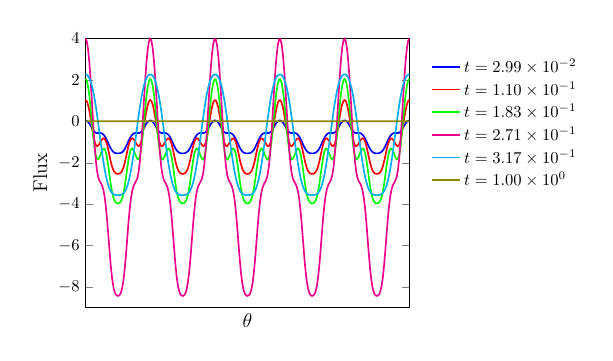
\begin{tikzpicture}[scale=0.6]

  \begin{axis}[
    xmin = 0,
    xmax = 6.2832,
    ymin = -9,
    ymax = 4,
    xtick = \empty,
    ylabel near ticks,
    xlabel = {\large $\theta$},
    ylabel = {\large Flux},
    clip = false,
    legend entries = {$t=2.99 \times 10^{-2}$,
    $t = 1.10 \times 10^{-1}$,
    $t = 1.83 \times 10^{-1}$,
    $t = 2.71 \times 10^{-1}$,
    $t = 3.17 \times 10^{-1}$,
    $t = 1.00 \times 10^{0}$},
    legend cell align=left,
    legend style={draw=none},
    legend style={at={(1.05,0.95)},anchor=north west}
  ]


\addplot[blue,line width=1pt] coordinates{
(0.0000e+00,4.3317e-02)
(2.4544e-02,2.5998e-02)
(4.9087e-02,-2.5040e-02)
(7.3631e-02,-1.0592e-01)
(9.8175e-02,-2.0844e-01)
(1.2272e-01,-3.1903e-01)
(1.4726e-01,-4.2115e-01)
(1.7181e-01,-4.9983e-01)
(1.9635e-01,-5.4734e-01)
(2.2089e-01,-5.6568e-01)
(2.4544e-01,-5.6530e-01)
(2.6998e-01,-5.6032e-01)
(2.9452e-01,-5.6394e-01)
(3.1907e-01,-5.8571e-01)
(3.4361e-01,-6.3142e-01)
(3.6816e-01,-7.0394e-01)
(3.9270e-01,-8.0342e-01)
(4.1724e-01,-9.2582e-01)
(4.4179e-01,-1.0617e+00)
(4.6633e-01,-1.1970e+00)
(4.9087e-01,-1.3173e+00)
(5.1542e-01,-1.4120e+00)
(5.3996e-01,-1.4782e+00)
(5.6450e-01,-1.5185e+00)
(5.8905e-01,-1.5399e+00)
(6.1359e-01,-1.5484e+00)
(6.3814e-01,-1.5494e+00)
(6.6268e-01,-1.5422e+00)
(6.8722e-01,-1.5242e+00)
(7.1177e-01,-1.4880e+00)
(7.3631e-01,-1.4276e+00)
(7.6085e-01,-1.3384e+00)
(7.8540e-01,-1.2228e+00)
(8.0994e-01,-1.0893e+00)
(8.3449e-01,-9.5236e-01)
(8.5903e-01,-8.2627e-01)
(8.8357e-01,-7.2174e-01)
(9.0812e-01,-6.4373e-01)
(9.3266e-01,-5.9279e-01)
(9.5720e-01,-5.6663e-01)
(9.8175e-01,-5.5996e-01)
(1.0063e+00,-5.6425e-01)
(1.0308e+00,-5.6662e-01)
(1.0554e+00,-5.5315e-01)
(1.0799e+00,-5.1185e-01)
(1.1045e+00,-4.3921e-01)
(1.1290e+00,-3.4060e-01)
(1.1536e+00,-2.3049e-01)
(1.1781e+00,-1.2499e-01)
(1.2026e+00,-3.9071e-02)
(1.2272e+00,1.8448e-02)
(1.2517e+00,4.2616e-02)
(1.2763e+00,3.2199e-02)
(1.3008e+00,-1.2223e-02)
(1.3254e+00,-8.7735e-02)
(1.3499e+00,-1.8672e-01)
(1.3744e+00,-2.9711e-01)
(1.3990e+00,-4.0213e-01)
(1.4235e+00,-4.8654e-01)
(1.4481e+00,-5.4032e-01)
(1.4726e+00,-5.6398e-01)
(1.4972e+00,-5.6616e-01)
(1.5217e+00,-5.6104e-01)
(1.5463e+00,-5.6198e-01)
(1.5708e+00,-5.7959e-01)
(1.5953e+00,-6.2017e-01)
(1.6199e+00,-6.8723e-01)
(1.6444e+00,-7.8150e-01)
(1.6690e+00,-8.9986e-01)
(1.6935e+00,-1.0342e+00)
(1.7181e+00,-1.1707e+00)
(1.7426e+00,-1.2951e+00)
(1.7671e+00,-1.3952e+00)
(1.7917e+00,-1.4673e+00)
(1.8162e+00,-1.5120e+00)
(1.8408e+00,-1.5370e+00)
(1.8653e+00,-1.5472e+00)
(1.8899e+00,-1.5500e+00)
(1.9144e+00,-1.5441e+00)
(1.9390e+00,-1.5292e+00)
(1.9635e+00,-1.4968e+00)
(1.9880e+00,-1.4420e+00)
(2.0126e+00,-1.3584e+00)
(2.0371e+00,-1.2478e+00)
(2.0617e+00,-1.1167e+00)
(2.0862e+00,-9.7934e-01)
(2.1108e+00,-8.5000e-01)
(2.1353e+00,-7.4061e-01)
(2.1598e+00,-6.5714e-01)
(2.1844e+00,-6.0088e-01)
(2.2089e+00,-5.7010e-01)
(2.2335e+00,-5.6006e-01)
(2.2580e+00,-5.6311e-01)
(2.2826e+00,-5.6694e-01)
(2.3071e+00,-5.5782e-01)
(2.3317e+00,-5.2259e-01)
(2.3562e+00,-4.5618e-01)
(2.3807e+00,-3.6172e-01)
(2.4053e+00,-2.5272e-01)
(2.4298e+00,-1.4487e-01)
(2.4544e+00,-5.4244e-02)
(2.4789e+00,9.5525e-03)
(2.5035e+00,4.0521e-02)
(2.5280e+00,3.7044e-02)
(2.5525e+00,-6.7853e-04)
(2.5771e+00,-7.0488e-02)
(2.6016e+00,-1.6549e-01)
(2.6262e+00,-2.7497e-01)
(2.6507e+00,-3.8227e-01)
(2.6753e+00,-4.7198e-01)
(2.6998e+00,-5.3208e-01)
(2.7243e+00,-5.6140e-01)
(2.7489e+00,-5.6675e-01)
(2.7734e+00,-5.6201e-01)
(2.7980e+00,-5.6071e-01)
(2.8225e+00,-5.7441e-01)
(2.8471e+00,-6.1000e-01)
(2.8716e+00,-6.7163e-01)
(2.8962e+00,-7.6055e-01)
(2.9207e+00,-8.7456e-01)
(2.9452e+00,-1.0066e+00)
(2.9698e+00,-1.1439e+00)
(2.9943e+00,-1.2719e+00)
(3.0189e+00,-1.3774e+00)
(3.0434e+00,-1.4552e+00)
(3.0680e+00,-1.5048e+00)
(3.0925e+00,-1.5335e+00)
(3.1170e+00,-1.5458e+00)
(3.1416e+00,-1.5502e+00)
(3.1661e+00,-1.5458e+00)
(3.1907e+00,-1.5335e+00)
(3.2152e+00,-1.5048e+00)
(3.2398e+00,-1.4552e+00)
(3.2643e+00,-1.3774e+00)
(3.2889e+00,-1.2719e+00)
(3.3134e+00,-1.1439e+00)
(3.3379e+00,-1.0066e+00)
(3.3625e+00,-8.7455e-01)
(3.3870e+00,-7.6055e-01)
(3.4116e+00,-6.7163e-01)
(3.4361e+00,-6.1000e-01)
(3.4607e+00,-5.7441e-01)
(3.4852e+00,-5.6071e-01)
(3.5097e+00,-5.6201e-01)
(3.5343e+00,-5.6675e-01)
(3.5588e+00,-5.6140e-01)
(3.5834e+00,-5.3208e-01)
(3.6079e+00,-4.7198e-01)
(3.6325e+00,-3.8227e-01)
(3.6570e+00,-2.7497e-01)
(3.6816e+00,-1.6549e-01)
(3.7061e+00,-7.0488e-02)
(3.7306e+00,-6.7871e-04)
(3.7552e+00,3.7044e-02)
(3.7797e+00,4.0521e-02)
(3.8043e+00,9.5528e-03)
(3.8288e+00,-5.4244e-02)
(3.8534e+00,-1.4487e-01)
(3.8779e+00,-2.5272e-01)
(3.9024e+00,-3.6172e-01)
(3.9270e+00,-4.5618e-01)
(3.9515e+00,-5.2259e-01)
(3.9761e+00,-5.5782e-01)
(4.0006e+00,-5.6694e-01)
(4.0252e+00,-5.6311e-01)
(4.0497e+00,-5.6006e-01)
(4.0743e+00,-5.7010e-01)
(4.0988e+00,-6.0088e-01)
(4.1233e+00,-6.5714e-01)
(4.1479e+00,-7.4062e-01)
(4.1724e+00,-8.5000e-01)
(4.1970e+00,-9.7934e-01)
(4.2215e+00,-1.1167e+00)
(4.2461e+00,-1.2478e+00)
(4.2706e+00,-1.3584e+00)
(4.2951e+00,-1.4420e+00)
(4.3197e+00,-1.4968e+00)
(4.3442e+00,-1.5292e+00)
(4.3688e+00,-1.5441e+00)
(4.3933e+00,-1.5500e+00)
(4.4179e+00,-1.5472e+00)
(4.4424e+00,-1.5370e+00)
(4.4670e+00,-1.5120e+00)
(4.4915e+00,-1.4673e+00)
(4.5160e+00,-1.3952e+00)
(4.5406e+00,-1.2951e+00)
(4.5651e+00,-1.1707e+00)
(4.5897e+00,-1.0342e+00)
(4.6142e+00,-8.9986e-01)
(4.6388e+00,-7.8150e-01)
(4.6633e+00,-6.8723e-01)
(4.6878e+00,-6.2017e-01)
(4.7124e+00,-5.7959e-01)
(4.7369e+00,-5.6198e-01)
(4.7615e+00,-5.6104e-01)
(4.7860e+00,-5.6616e-01)
(4.8106e+00,-5.6398e-01)
(4.8351e+00,-5.4032e-01)
(4.8597e+00,-4.8654e-01)
(4.8842e+00,-4.0213e-01)
(4.9087e+00,-2.9711e-01)
(4.9333e+00,-1.8672e-01)
(4.9578e+00,-8.7735e-02)
(4.9824e+00,-1.2223e-02)
(5.0069e+00,3.2199e-02)
(5.0315e+00,4.2616e-02)
(5.0560e+00,1.8448e-02)
(5.0805e+00,-3.9071e-02)
(5.1051e+00,-1.2499e-01)
(5.1296e+00,-2.3049e-01)
(5.1542e+00,-3.4060e-01)
(5.1787e+00,-4.3921e-01)
(5.2033e+00,-5.1185e-01)
(5.2278e+00,-5.5315e-01)
(5.2524e+00,-5.6662e-01)
(5.2769e+00,-5.6425e-01)
(5.3014e+00,-5.5996e-01)
(5.3260e+00,-5.6663e-01)
(5.3505e+00,-5.9279e-01)
(5.3751e+00,-6.4373e-01)
(5.3996e+00,-7.2174e-01)
(5.4242e+00,-8.2627e-01)
(5.4487e+00,-9.5236e-01)
(5.4732e+00,-1.0893e+00)
(5.4978e+00,-1.2228e+00)
(5.5223e+00,-1.3384e+00)
(5.5469e+00,-1.4276e+00)
(5.5714e+00,-1.4880e+00)
(5.5960e+00,-1.5242e+00)
(5.6205e+00,-1.5422e+00)
(5.6450e+00,-1.5494e+00)
(5.6696e+00,-1.5484e+00)
(5.6941e+00,-1.5399e+00)
(5.7187e+00,-1.5185e+00)
(5.7432e+00,-1.4782e+00)
(5.7678e+00,-1.4120e+00)
(5.7923e+00,-1.3173e+00)
(5.8169e+00,-1.1970e+00)
(5.8414e+00,-1.0617e+00)
(5.8659e+00,-9.2582e-01)
(5.8905e+00,-8.0342e-01)
(5.9150e+00,-7.0394e-01)
(5.9396e+00,-6.3142e-01)
(5.9641e+00,-5.8571e-01)
(5.9887e+00,-5.6394e-01)
(6.0132e+00,-5.6032e-01)
(6.0377e+00,-5.6530e-01)
(6.0623e+00,-5.6568e-01)
(6.0868e+00,-5.4734e-01)
(6.1114e+00,-4.9983e-01)
(6.1359e+00,-4.2115e-01)
(6.1605e+00,-3.1903e-01)
(6.1850e+00,-2.0844e-01)
(6.2096e+00,-1.0592e-01)
(6.2341e+00,-2.5040e-02)
(6.2586e+00,2.5998e-02)
(6.2832e+00,4.3317e-02)
};

\addplot[red,line width=1pt] coordinates{
(0.0000e+00,1.0315e+00)
(2.4544e-02,9.7196e-01)
(4.9087e-02,7.9557e-01)
(7.3631e-02,5.1327e-01)
(9.8175e-02,1.4973e-01)
(1.2272e-01,-2.5148e-01)
(1.4726e-01,-6.3351e-01)
(1.7181e-01,-9.3940e-01)
(1.9635e-01,-1.1313e+00)
(2.2089e-01,-1.2017e+00)
(2.4544e-01,-1.1725e+00)
(2.6998e-01,-1.0823e+00)
(2.9452e-01,-9.7242e-01)
(3.1907e-01,-8.7733e-01)
(3.4361e-01,-8.2501e-01)
(3.6816e-01,-8.3886e-01)
(3.9270e-01,-9.3717e-01)
(4.1724e-01,-1.1244e+00)
(4.4179e-01,-1.3839e+00)
(4.6633e-01,-1.6771e+00)
(4.9087e-01,-1.9585e+00)
(5.1542e-01,-2.1904e+00)
(5.3996e-01,-2.3570e+00)
(5.6450e-01,-2.4599e+00)
(5.8905e-01,-2.5151e+00)
(6.1359e-01,-2.5370e+00)
(6.3814e-01,-2.5398e+00)
(6.6268e-01,-2.5209e+00)
(6.8722e-01,-2.4749e+00)
(7.1177e-01,-2.3818e+00)
(7.3631e-01,-2.2295e+00)
(7.6085e-01,-2.0094e+00)
(7.8540e-01,-1.7360e+00)
(8.0994e-01,-1.4411e+00)
(8.3449e-01,-1.1716e+00)
(8.5903e-01,-9.6761e-01)
(8.8357e-01,-8.5140e-01)
(9.0812e-01,-8.2180e-01)
(9.3266e-01,-8.6260e-01)
(9.5720e-01,-9.5131e-01)
(9.8175e-01,-1.0606e+00)
(1.0063e+00,-1.1581e+00)
(1.0308e+00,-1.2025e+00)
(1.0554e+00,-1.1550e+00)
(1.0799e+00,-9.8741e-01)
(1.1045e+00,-7.0261e-01)
(1.1290e+00,-3.3111e-01)
(1.1536e+00,7.0559e-02)
(1.1781e+00,4.4617e-01)
(1.2026e+00,7.4685e-01)
(1.2272e+00,9.4595e-01)
(1.2517e+00,1.0291e+00)
(1.2763e+00,9.9330e-01)
(1.3008e+00,8.3999e-01)
(1.3254e+00,5.7706e-01)
(1.3499e+00,2.2734e-01)
(1.3744e+00,-1.7109e-01)
(1.3990e+00,-5.6129e-01)
(1.4235e+00,-8.8675e-01)
(1.4481e+00,-1.1027e+00)
(1.4726e+00,-1.1968e+00)
(1.4972e+00,-1.1844e+00)
(1.5217e+00,-1.1033e+00)
(1.5463e+00,-9.9412e-01)
(1.5708e+00,-8.9380e-01)
(1.5953e+00,-8.3086e-01)
(1.6199e+00,-8.2977e-01)
(1.6444e+00,-9.1033e-01)
(1.6690e+00,-1.0802e+00)
(1.6935e+00,-1.3280e+00)
(1.7181e+00,-1.6177e+00)
(1.7426e+00,-1.9056e+00)
(1.7671e+00,-2.1486e+00)
(1.7917e+00,-2.3296e+00)
(1.8162e+00,-2.4431e+00)
(1.8408e+00,-2.5079e+00)
(1.8653e+00,-2.5337e+00)
(1.8899e+00,-2.5416e+00)
(1.9144e+00,-2.5257e+00)
(1.9390e+00,-2.4879e+00)
(1.9635e+00,-2.4042e+00)
(1.9880e+00,-2.2658e+00)
(2.0126e+00,-2.0580e+00)
(2.0371e+00,-1.7940e+00)
(2.0617e+00,-1.4994e+00)
(2.0862e+00,-1.2215e+00)
(2.1108e+00,-1.0016e+00)
(2.1353e+00,-8.6746e-01)
(2.1598e+00,-8.2140e-01)
(2.1844e+00,-8.4982e-01)
(2.2089e+00,-9.3102e-01)
(2.2335e+00,-1.0385e+00)
(2.2580e+00,-1.1415e+00)
(2.2826e+00,-1.1997e+00)
(2.3071e+00,-1.1737e+00)
(2.3317e+00,-1.0307e+00)
(2.3562e+00,-7.6810e-01)
(2.3807e+00,-4.0959e-01)
(2.4053e+00,-9.6323e-03)
(2.4298e+00,3.7596e-01)
(2.4544e+00,6.9405e-01)
(2.4789e+00,9.1527e-01)
(2.5035e+00,1.0219e+00)
(2.5280e+00,1.0100e+00)
(2.5525e+00,8.7993e-01)
(2.5771e+00,6.3738e-01)
(2.6016e+00,3.0290e-01)
(2.6262e+00,-9.0337e-02)
(2.6507e+00,-4.8648e-01)
(2.6753e+00,-8.2958e-01)
(2.6998e+00,-1.0691e+00)
(2.7243e+00,-1.1876e+00)
(2.7489e+00,-1.1936e+00)
(2.7734e+00,-1.1231e+00)
(2.7980e+00,-1.0162e+00)
(2.8225e+00,-9.1177e-01)
(2.8471e+00,-8.3919e-01)
(2.8716e+00,-8.2400e-01)
(2.8962e+00,-8.8710e-01)
(2.9207e+00,-1.0392e+00)
(2.9452e+00,-1.2738e+00)
(2.9698e+00,-1.5584e+00)
(2.9943e+00,-1.8507e+00)
(3.0189e+00,-2.1045e+00)
(3.0434e+00,-2.2992e+00)
(3.0680e+00,-2.4246e+00)
(3.0925e+00,-2.4989e+00)
(3.1170e+00,-2.5299e+00)
(3.1416e+00,-2.5423e+00)
(3.1661e+00,-2.5299e+00)
(3.1907e+00,-2.4989e+00)
(3.2152e+00,-2.4246e+00)
(3.2398e+00,-2.2992e+00)
(3.2643e+00,-2.1045e+00)
(3.2889e+00,-1.8507e+00)
(3.3134e+00,-1.5584e+00)
(3.3379e+00,-1.2738e+00)
(3.3625e+00,-1.0392e+00)
(3.3870e+00,-8.8710e-01)
(3.4116e+00,-8.2400e-01)
(3.4361e+00,-8.3919e-01)
(3.4607e+00,-9.1177e-01)
(3.4852e+00,-1.0162e+00)
(3.5097e+00,-1.1231e+00)
(3.5343e+00,-1.1936e+00)
(3.5588e+00,-1.1876e+00)
(3.5834e+00,-1.0691e+00)
(3.6079e+00,-8.2958e-01)
(3.6325e+00,-4.8648e-01)
(3.6570e+00,-9.0337e-02)
(3.6816e+00,3.0290e-01)
(3.7061e+00,6.3738e-01)
(3.7306e+00,8.7993e-01)
(3.7552e+00,1.0100e+00)
(3.7797e+00,1.0219e+00)
(3.8043e+00,9.1527e-01)
(3.8288e+00,6.9405e-01)
(3.8534e+00,3.7596e-01)
(3.8779e+00,-9.6323e-03)
(3.9024e+00,-4.0959e-01)
(3.9270e+00,-7.6810e-01)
(3.9515e+00,-1.0307e+00)
(3.9761e+00,-1.1737e+00)
(4.0006e+00,-1.1997e+00)
(4.0252e+00,-1.1415e+00)
(4.0497e+00,-1.0385e+00)
(4.0743e+00,-9.3102e-01)
(4.0988e+00,-8.4982e-01)
(4.1233e+00,-8.2140e-01)
(4.1479e+00,-8.6746e-01)
(4.1724e+00,-1.0016e+00)
(4.1970e+00,-1.2215e+00)
(4.2215e+00,-1.4994e+00)
(4.2461e+00,-1.7940e+00)
(4.2706e+00,-2.0580e+00)
(4.2951e+00,-2.2658e+00)
(4.3197e+00,-2.4042e+00)
(4.3442e+00,-2.4879e+00)
(4.3688e+00,-2.5257e+00)
(4.3933e+00,-2.5416e+00)
(4.4179e+00,-2.5337e+00)
(4.4424e+00,-2.5079e+00)
(4.4670e+00,-2.4431e+00)
(4.4915e+00,-2.3296e+00)
(4.5160e+00,-2.1486e+00)
(4.5406e+00,-1.9056e+00)
(4.5651e+00,-1.6177e+00)
(4.5897e+00,-1.3280e+00)
(4.6142e+00,-1.0802e+00)
(4.6388e+00,-9.1033e-01)
(4.6633e+00,-8.2977e-01)
(4.6878e+00,-8.3086e-01)
(4.7124e+00,-8.9380e-01)
(4.7369e+00,-9.9412e-01)
(4.7615e+00,-1.1033e+00)
(4.7860e+00,-1.1844e+00)
(4.8106e+00,-1.1968e+00)
(4.8351e+00,-1.1027e+00)
(4.8597e+00,-8.8675e-01)
(4.8842e+00,-5.6129e-01)
(4.9087e+00,-1.7109e-01)
(4.9333e+00,2.2734e-01)
(4.9578e+00,5.7706e-01)
(4.9824e+00,8.3999e-01)
(5.0069e+00,9.9330e-01)
(5.0315e+00,1.0291e+00)
(5.0560e+00,9.4595e-01)
(5.0805e+00,7.4685e-01)
(5.1051e+00,4.4617e-01)
(5.1296e+00,7.0559e-02)
(5.1542e+00,-3.3111e-01)
(5.1787e+00,-7.0261e-01)
(5.2033e+00,-9.8741e-01)
(5.2278e+00,-1.1550e+00)
(5.2524e+00,-1.2025e+00)
(5.2769e+00,-1.1581e+00)
(5.3014e+00,-1.0606e+00)
(5.3260e+00,-9.5131e-01)
(5.3505e+00,-8.6260e-01)
(5.3751e+00,-8.2180e-01)
(5.3996e+00,-8.5140e-01)
(5.4242e+00,-9.6761e-01)
(5.4487e+00,-1.1716e+00)
(5.4732e+00,-1.4411e+00)
(5.4978e+00,-1.7360e+00)
(5.5223e+00,-2.0094e+00)
(5.5469e+00,-2.2295e+00)
(5.5714e+00,-2.3818e+00)
(5.5960e+00,-2.4749e+00)
(5.6205e+00,-2.5209e+00)
(5.6450e+00,-2.5398e+00)
(5.6696e+00,-2.5370e+00)
(5.6941e+00,-2.5151e+00)
(5.7187e+00,-2.4599e+00)
(5.7432e+00,-2.3570e+00)
(5.7678e+00,-2.1904e+00)
(5.7923e+00,-1.9585e+00)
(5.8169e+00,-1.6771e+00)
(5.8414e+00,-1.3839e+00)
(5.8659e+00,-1.1244e+00)
(5.8905e+00,-9.3717e-01)
(5.9150e+00,-8.3886e-01)
(5.9396e+00,-8.2501e-01)
(5.9641e+00,-8.7733e-01)
(5.9887e+00,-9.7242e-01)
(6.0132e+00,-1.0823e+00)
(6.0377e+00,-1.1725e+00)
(6.0623e+00,-1.2017e+00)
(6.0868e+00,-1.1313e+00)
(6.1114e+00,-9.3940e-01)
(6.1359e+00,-6.3351e-01)
(6.1605e+00,-2.5148e-01)
(6.1850e+00,1.4973e-01)
(6.2096e+00,5.1327e-01)
(6.2341e+00,7.9557e-01)
(6.2586e+00,9.7196e-01)
(6.2832e+00,1.0315e+00)
};

\addplot[green,line width=1pt] coordinates{
(0.0000e+00,2.0503e+00)
(2.4544e-02,1.9579e+00)
(4.9087e-02,1.6826e+00)
(7.3631e-02,1.2369e+00)
(9.8175e-02,6.5244e-01)
(1.2272e-01,-1.0525e-02)
(1.4726e-01,-6.6768e-01)
(1.7181e-01,-1.2271e+00)
(1.9635e-01,-1.6187e+00)
(2.2089e-01,-1.8145e+00)
(2.4544e-01,-1.8351e+00)
(2.6998e-01,-1.7337e+00)
(2.9452e-01,-1.5761e+00)
(3.1907e-01,-1.4227e+00)
(3.4361e-01,-1.3265e+00)
(3.6816e-01,-1.3323e+00)
(3.9270e-01,-1.4744e+00)
(4.1724e-01,-1.7612e+00)
(4.4179e-01,-2.1652e+00)
(4.6633e-01,-2.6230e+00)
(4.9087e-01,-3.0621e+00)
(5.1542e-01,-3.4228e+00)
(5.3996e-01,-3.6817e+00)
(5.6450e-01,-3.8410e+00)
(5.8905e-01,-3.9267e+00)
(6.1359e-01,-3.9605e+00)
(6.3814e-01,-3.9649e+00)
(6.6268e-01,-3.9355e+00)
(6.8722e-01,-3.8644e+00)
(7.1177e-01,-3.7199e+00)
(7.3631e-01,-3.4837e+00)
(7.6085e-01,-3.1411e+00)
(7.8540e-01,-2.7151e+00)
(8.0994e-01,-2.2545e+00)
(8.3449e-01,-1.8345e+00)
(8.5903e-01,-1.5203e+00)
(8.8357e-01,-1.3491e+00)
(9.0812e-01,-1.3182e+00)
(9.3266e-01,-1.3973e+00)
(9.5720e-01,-1.5434e+00)
(9.8175e-01,-1.7045e+00)
(1.0063e+00,-1.8227e+00)
(1.0308e+00,-1.8310e+00)
(1.0554e+00,-1.6739e+00)
(1.0799e+00,-1.3201e+00)
(1.1045e+00,-7.9051e-01)
(1.1290e+00,-1.4500e-01)
(1.1536e+00,5.2329e-01)
(1.1781e+00,1.1300e+00)
(1.2026e+00,1.6061e+00)
(1.2272e+00,1.9174e+00)
(1.2517e+00,2.0466e+00)
(1.2763e+00,1.9910e+00)
(1.3008e+00,1.7521e+00)
(1.3254e+00,1.3382e+00)
(1.3499e+00,7.7837e-01)
(1.3744e+00,1.2414e-01)
(1.3990e+00,-5.4084e-01)
(1.4235e+00,-1.1273e+00)
(1.4481e+00,-1.5556e+00)
(1.4726e+00,-1.7909e+00)
(1.4972e+00,-1.8425e+00)
(1.5217e+00,-1.7608e+00)
(1.5463e+00,-1.6090e+00)
(1.5708e+00,-1.4505e+00)
(1.5953e+00,-1.3390e+00)
(1.6199e+00,-1.3210e+00)
(1.6444e+00,-1.4343e+00)
(1.6690e+00,-1.6927e+00)
(1.6935e+00,-2.0781e+00)
(1.7181e+00,-2.5302e+00)
(1.7426e+00,-2.9797e+00)
(1.7671e+00,-3.3577e+00)
(1.7917e+00,-3.6392e+00)
(1.8162e+00,-3.8149e+00)
(1.8408e+00,-3.9157e+00)
(1.8653e+00,-3.9552e+00)
(1.8899e+00,-3.9678e+00)
(1.9144e+00,-3.9428e+00)
(1.9390e+00,-3.8847e+00)
(1.9635e+00,-3.7545e+00)
(1.9880e+00,-3.5403e+00)
(2.0126e+00,-3.2168e+00)
(2.0371e+00,-2.8057e+00)
(2.0617e+00,-2.3454e+00)
(2.0862e+00,-1.9122e+00)
(2.1108e+00,-1.5721e+00)
(2.1353e+00,-1.3717e+00)
(2.1598e+00,-1.3142e+00)
(2.1844e+00,-1.3747e+00)
(2.2089e+00,-1.5113e+00)
(2.2335e+00,-1.6736e+00)
(2.2580e+00,-1.8059e+00)
(2.2826e+00,-1.8409e+00)
(2.3071e+00,-1.7209e+00)
(2.3317e+00,-1.4060e+00)
(2.3562e+00,-9.0851e-01)
(2.3807e+00,-2.7869e-01)
(2.4053e+00,3.9170e-01)
(2.4298e+00,1.0177e+00)
(2.4544e+00,1.5230e+00)
(2.4789e+00,1.8696e+00)
(2.5035e+00,2.0354e+00)
(2.5280e+00,2.0169e+00)
(2.5525e+00,1.8145e+00)
(2.5771e+00,1.4336e+00)
(2.6016e+00,9.0034e-01)
(2.6262e+00,2.5842e-01)
(2.6507e+00,-4.1089e-01)
(2.6753e+00,-1.0210e+00)
(2.6998e+00,-1.4846e+00)
(2.7243e+00,-1.7598e+00)
(2.7489e+00,-1.8446e+00)
(2.7734e+00,-1.7850e+00)
(2.7980e+00,-1.6416e+00)
(2.8225e+00,-1.4801e+00)
(2.8471e+00,-1.3551e+00)
(2.8716e+00,-1.3150e+00)
(2.8962e+00,-1.4001e+00)
(2.9207e+00,-1.6296e+00)
(2.9452e+00,-1.9936e+00)
(2.9698e+00,-2.4375e+00)
(2.9943e+00,-2.8941e+00)
(3.0189e+00,-3.2890e+00)
(3.0434e+00,-3.5921e+00)
(3.0680e+00,-3.7861e+00)
(3.0925e+00,-3.9018e+00)
(3.1170e+00,-3.9493e+00)
(3.1416e+00,-3.9688e+00)
(3.1661e+00,-3.9493e+00)
(3.1907e+00,-3.9018e+00)
(3.2152e+00,-3.7861e+00)
(3.2398e+00,-3.5921e+00)
(3.2643e+00,-3.2890e+00)
(3.2889e+00,-2.8941e+00)
(3.3134e+00,-2.4375e+00)
(3.3379e+00,-1.9936e+00)
(3.3625e+00,-1.6296e+00)
(3.3870e+00,-1.4001e+00)
(3.4116e+00,-1.3150e+00)
(3.4361e+00,-1.3551e+00)
(3.4607e+00,-1.4801e+00)
(3.4852e+00,-1.6416e+00)
(3.5097e+00,-1.7850e+00)
(3.5343e+00,-1.8446e+00)
(3.5588e+00,-1.7598e+00)
(3.5834e+00,-1.4846e+00)
(3.6079e+00,-1.0210e+00)
(3.6325e+00,-4.1090e-01)
(3.6570e+00,2.5842e-01)
(3.6816e+00,9.0034e-01)
(3.7061e+00,1.4336e+00)
(3.7306e+00,1.8145e+00)
(3.7552e+00,2.0169e+00)
(3.7797e+00,2.0354e+00)
(3.8043e+00,1.8696e+00)
(3.8288e+00,1.5230e+00)
(3.8534e+00,1.0177e+00)
(3.8779e+00,3.9170e-01)
(3.9024e+00,-2.7869e-01)
(3.9270e+00,-9.0851e-01)
(3.9515e+00,-1.4060e+00)
(3.9761e+00,-1.7209e+00)
(4.0006e+00,-1.8409e+00)
(4.0252e+00,-1.8059e+00)
(4.0497e+00,-1.6736e+00)
(4.0743e+00,-1.5113e+00)
(4.0988e+00,-1.3747e+00)
(4.1233e+00,-1.3142e+00)
(4.1479e+00,-1.3717e+00)
(4.1724e+00,-1.5721e+00)
(4.1970e+00,-1.9122e+00)
(4.2215e+00,-2.3454e+00)
(4.2461e+00,-2.8057e+00)
(4.2706e+00,-3.2168e+00)
(4.2951e+00,-3.5403e+00)
(4.3197e+00,-3.7545e+00)
(4.3442e+00,-3.8847e+00)
(4.3688e+00,-3.9428e+00)
(4.3933e+00,-3.9678e+00)
(4.4179e+00,-3.9552e+00)
(4.4424e+00,-3.9157e+00)
(4.4670e+00,-3.8149e+00)
(4.4915e+00,-3.6392e+00)
(4.5160e+00,-3.3577e+00)
(4.5406e+00,-2.9797e+00)
(4.5651e+00,-2.5302e+00)
(4.5897e+00,-2.0781e+00)
(4.6142e+00,-1.6927e+00)
(4.6388e+00,-1.4343e+00)
(4.6633e+00,-1.3210e+00)
(4.6878e+00,-1.3390e+00)
(4.7124e+00,-1.4505e+00)
(4.7369e+00,-1.6090e+00)
(4.7615e+00,-1.7608e+00)
(4.7860e+00,-1.8425e+00)
(4.8106e+00,-1.7909e+00)
(4.8351e+00,-1.5556e+00)
(4.8597e+00,-1.1273e+00)
(4.8842e+00,-5.4084e-01)
(4.9087e+00,1.2414e-01)
(4.9333e+00,7.7837e-01)
(4.9578e+00,1.3382e+00)
(4.9824e+00,1.7521e+00)
(5.0069e+00,1.9910e+00)
(5.0315e+00,2.0466e+00)
(5.0560e+00,1.9174e+00)
(5.0805e+00,1.6061e+00)
(5.1051e+00,1.1300e+00)
(5.1296e+00,5.2329e-01)
(5.1542e+00,-1.4500e-01)
(5.1787e+00,-7.9051e-01)
(5.2033e+00,-1.3201e+00)
(5.2278e+00,-1.6739e+00)
(5.2524e+00,-1.8310e+00)
(5.2769e+00,-1.8227e+00)
(5.3014e+00,-1.7045e+00)
(5.3260e+00,-1.5434e+00)
(5.3505e+00,-1.3973e+00)
(5.3751e+00,-1.3182e+00)
(5.3996e+00,-1.3491e+00)
(5.4242e+00,-1.5203e+00)
(5.4487e+00,-1.8345e+00)
(5.4732e+00,-2.2545e+00)
(5.4978e+00,-2.7151e+00)
(5.5223e+00,-3.1411e+00)
(5.5469e+00,-3.4837e+00)
(5.5714e+00,-3.7199e+00)
(5.5960e+00,-3.8644e+00)
(5.6205e+00,-3.9355e+00)
(5.6450e+00,-3.9649e+00)
(5.6696e+00,-3.9605e+00)
(5.6941e+00,-3.9267e+00)
(5.7187e+00,-3.8410e+00)
(5.7432e+00,-3.6817e+00)
(5.7678e+00,-3.4228e+00)
(5.7923e+00,-3.0621e+00)
(5.8169e+00,-2.6230e+00)
(5.8414e+00,-2.1652e+00)
(5.8659e+00,-1.7612e+00)
(5.8905e+00,-1.4744e+00)
(5.9150e+00,-1.3323e+00)
(5.9396e+00,-1.3265e+00)
(5.9641e+00,-1.4227e+00)
(5.9887e+00,-1.5761e+00)
(6.0132e+00,-1.7337e+00)
(6.0377e+00,-1.8351e+00)
(6.0623e+00,-1.8145e+00)
(6.0868e+00,-1.6187e+00)
(6.1114e+00,-1.2271e+00)
(6.1359e+00,-6.6768e-01)
(6.1605e+00,-1.0525e-02)
(6.1850e+00,6.5244e-01)
(6.2096e+00,1.2369e+00)
(6.2341e+00,1.6826e+00)
(6.2586e+00,1.9579e+00)
(6.2832e+00,2.0503e+00)
};

\addplot[magenta,line width=1pt] coordinates{
(0.0000e+00,3.9993e+00)
(2.4544e-02,3.8712e+00)
(4.9087e-02,3.4877e+00)
(7.3631e-02,2.8573e+00)
(9.8175e-02,2.0100e+00)
(1.2272e-01,1.0122e+00)
(1.4726e-01,-3.3804e-02)
(1.7181e-01,-1.0057e+00)
(1.9635e-01,-1.7982e+00)
(2.2089e-01,-2.3554e+00)
(2.4544e-01,-2.6897e+00)
(2.6998e-01,-2.8661e+00)
(2.9452e-01,-2.9732e+00)
(3.1907e-01,-3.0909e+00)
(3.4361e-01,-3.2837e+00)
(3.6816e-01,-3.6001e+00)
(3.9270e-01,-4.0770e+00)
(4.1724e-01,-4.7175e+00)
(4.4179e-01,-5.4796e+00)
(4.6633e-01,-6.2730e+00)
(4.9087e-01,-6.9993e+00)
(5.1542e-01,-7.5802e+00)
(5.3996e-01,-7.9905e+00)
(5.6450e-01,-8.2411e+00)
(5.8905e-01,-8.3747e+00)
(6.1359e-01,-8.4281e+00)
(6.3814e-01,-8.4340e+00)
(6.6268e-01,-8.3891e+00)
(6.8722e-01,-8.2773e+00)
(7.1177e-01,-8.0510e+00)
(7.3631e-01,-7.6771e+00)
(7.6085e-01,-7.1278e+00)
(7.8540e-01,-6.4275e+00)
(8.0994e-01,-5.6385e+00)
(8.3449e-01,-4.8630e+00)
(8.5903e-01,-4.1923e+00)
(8.8357e-01,-3.6822e+00)
(9.0812e-01,-3.3355e+00)
(9.3266e-01,-3.1217e+00)
(9.5720e-01,-2.9937e+00)
(9.8175e-01,-2.8900e+00)
(1.0063e+00,-2.7351e+00)
(1.0308e+00,-2.4382e+00)
(1.0554e+00,-1.9294e+00)
(1.0799e+00,-1.1808e+00)
(1.1045e+00,-2.3848e-01)
(1.1290e+00,8.0355e-01)
(1.1536e+00,1.8192e+00)
(1.1781e+00,2.7041e+00)
(1.2026e+00,3.3804e+00)
(1.2272e+00,3.8151e+00)
(1.2517e+00,3.9941e+00)
(1.2763e+00,3.9172e+00)
(1.3008e+00,3.5850e+00)
(1.3254e+00,3.0017e+00)
(1.3499e+00,2.1947e+00)
(1.3744e+00,1.2188e+00)
(1.3990e+00,1.7391e-01)
(1.4235e+00,-8.2334e-01)
(1.4481e+00,-1.6572e+00)
(1.4726e+00,-2.2634e+00)
(1.4972e+00,-2.6378e+00)
(1.5217e+00,-2.8394e+00)
(1.5463e+00,-2.9531e+00)
(1.5708e+00,-3.0632e+00)
(1.5953e+00,-3.2367e+00)
(1.6199e+00,-3.5247e+00)
(1.6444e+00,-3.9684e+00)
(1.6690e+00,-4.5771e+00)
(1.6935e+00,-5.3219e+00)
(1.7181e+00,-6.1160e+00)
(1.7426e+00,-6.8648e+00)
(1.7671e+00,-7.4764e+00)
(1.7917e+00,-7.9234e+00)
(1.8162e+00,-8.2003e+00)
(1.8408e+00,-8.3570e+00)
(1.8653e+00,-8.4205e+00)
(1.8899e+00,-8.4378e+00)
(1.9144e+00,-8.4011e+00)
(1.9390e+00,-8.3087e+00)
(1.9635e+00,-8.1057e+00)
(1.9880e+00,-7.7668e+00)
(2.0126e+00,-7.2501e+00)
(2.0371e+00,-6.5782e+00)
(2.0617e+00,-5.7979e+00)
(2.0862e+00,-5.0128e+00)
(2.1108e+00,-4.3142e+00)
(2.1353e+00,-3.7709e+00)
(2.1598e+00,-3.3927e+00)
(2.1844e+00,-3.1560e+00)
(2.2089e+00,-3.0151e+00)
(2.2335e+00,-2.9121e+00)
(2.2580e+00,-2.7748e+00)
(2.2826e+00,-2.5126e+00)
(2.3071e+00,-2.0507e+00)
(2.3317e+00,-1.3480e+00)
(2.3562e+00,-4.3895e-01)
(2.3807e+00,5.9368e-01)
(2.4053e+00,1.6231e+00)
(2.4298e+00,2.5424e+00)
(2.4544e+00,3.2635e+00)
(2.4789e+00,3.7487e+00)
(2.5035e+00,3.9787e+00)
(2.5280e+00,3.9530e+00)
(2.5525e+00,3.6720e+00)
(2.5771e+00,3.1371e+00)
(2.6016e+00,2.3724e+00)
(2.6262e+00,1.4227e+00)
(2.6507e+00,3.8346e-01)
(2.6753e+00,-6.3419e-01)
(2.6998e+00,-1.5070e+00)
(2.7243e+00,-2.1620e+00)
(2.7489e+00,-2.5789e+00)
(2.7734e+00,-2.8093e+00)
(2.7980e+00,-2.9329e+00)
(2.8225e+00,-3.0381e+00)
(2.8471e+00,-3.1943e+00)
(2.8716e+00,-3.4557e+00)
(2.8962e+00,-3.8663e+00)
(2.9207e+00,-4.4425e+00)
(2.9452e+00,-5.1661e+00)
(2.9698e+00,-5.9573e+00)
(2.9943e+00,-6.7242e+00)
(3.0189e+00,-7.3663e+00)
(3.0434e+00,-7.8489e+00)
(3.0680e+00,-8.1553e+00)
(3.0925e+00,-8.3352e+00)
(3.1170e+00,-8.4114e+00)
(3.1416e+00,-8.4391e+00)
(3.1661e+00,-8.4114e+00)
(3.1907e+00,-8.3353e+00)
(3.2152e+00,-8.1553e+00)
(3.2398e+00,-7.8489e+00)
(3.2643e+00,-7.3663e+00)
(3.2889e+00,-6.7242e+00)
(3.3134e+00,-5.9573e+00)
(3.3379e+00,-5.1661e+00)
(3.3625e+00,-4.4425e+00)
(3.3870e+00,-3.8663e+00)
(3.4116e+00,-3.4557e+00)
(3.4361e+00,-3.1943e+00)
(3.4607e+00,-3.0381e+00)
(3.4852e+00,-2.9329e+00)
(3.5097e+00,-2.8093e+00)
(3.5343e+00,-2.5789e+00)
(3.5588e+00,-2.1620e+00)
(3.5834e+00,-1.5070e+00)
(3.6079e+00,-6.3419e-01)
(3.6325e+00,3.8346e-01)
(3.6570e+00,1.4227e+00)
(3.6816e+00,2.3724e+00)
(3.7061e+00,3.1371e+00)
(3.7306e+00,3.6720e+00)
(3.7552e+00,3.9530e+00)
(3.7797e+00,3.9787e+00)
(3.8043e+00,3.7487e+00)
(3.8288e+00,3.2635e+00)
(3.8534e+00,2.5424e+00)
(3.8779e+00,1.6231e+00)
(3.9024e+00,5.9368e-01)
(3.9270e+00,-4.3895e-01)
(3.9515e+00,-1.3480e+00)
(3.9761e+00,-2.0507e+00)
(4.0006e+00,-2.5126e+00)
(4.0252e+00,-2.7748e+00)
(4.0497e+00,-2.9121e+00)
(4.0743e+00,-3.0151e+00)
(4.0988e+00,-3.1560e+00)
(4.1233e+00,-3.3927e+00)
(4.1479e+00,-3.7709e+00)
(4.1724e+00,-4.3142e+00)
(4.1970e+00,-5.0128e+00)
(4.2215e+00,-5.7979e+00)
(4.2461e+00,-6.5782e+00)
(4.2706e+00,-7.2501e+00)
(4.2951e+00,-7.7668e+00)
(4.3197e+00,-8.1057e+00)
(4.3442e+00,-8.3087e+00)
(4.3688e+00,-8.4011e+00)
(4.3933e+00,-8.4378e+00)
(4.4179e+00,-8.4205e+00)
(4.4424e+00,-8.3570e+00)
(4.4670e+00,-8.2003e+00)
(4.4915e+00,-7.9234e+00)
(4.5160e+00,-7.4764e+00)
(4.5406e+00,-6.8648e+00)
(4.5651e+00,-6.1160e+00)
(4.5897e+00,-5.3219e+00)
(4.6142e+00,-4.5771e+00)
(4.6388e+00,-3.9684e+00)
(4.6633e+00,-3.5247e+00)
(4.6878e+00,-3.2367e+00)
(4.7124e+00,-3.0632e+00)
(4.7369e+00,-2.9531e+00)
(4.7615e+00,-2.8394e+00)
(4.7860e+00,-2.6378e+00)
(4.8106e+00,-2.2634e+00)
(4.8351e+00,-1.6572e+00)
(4.8597e+00,-8.2334e-01)
(4.8842e+00,1.7391e-01)
(4.9087e+00,1.2188e+00)
(4.9333e+00,2.1947e+00)
(4.9578e+00,3.0017e+00)
(4.9824e+00,3.5850e+00)
(5.0069e+00,3.9172e+00)
(5.0315e+00,3.9941e+00)
(5.0560e+00,3.8151e+00)
(5.0805e+00,3.3804e+00)
(5.1051e+00,2.7041e+00)
(5.1296e+00,1.8192e+00)
(5.1542e+00,8.0355e-01)
(5.1787e+00,-2.3848e-01)
(5.2033e+00,-1.1808e+00)
(5.2278e+00,-1.9294e+00)
(5.2524e+00,-2.4382e+00)
(5.2769e+00,-2.7351e+00)
(5.3014e+00,-2.8900e+00)
(5.3260e+00,-2.9937e+00)
(5.3505e+00,-3.1217e+00)
(5.3751e+00,-3.3355e+00)
(5.3996e+00,-3.6822e+00)
(5.4242e+00,-4.1923e+00)
(5.4487e+00,-4.8630e+00)
(5.4732e+00,-5.6385e+00)
(5.4978e+00,-6.4275e+00)
(5.5223e+00,-7.1278e+00)
(5.5469e+00,-7.6771e+00)
(5.5714e+00,-8.0510e+00)
(5.5960e+00,-8.2773e+00)
(5.6205e+00,-8.3891e+00)
(5.6450e+00,-8.4340e+00)
(5.6696e+00,-8.4281e+00)
(5.6941e+00,-8.3747e+00)
(5.7187e+00,-8.2411e+00)
(5.7432e+00,-7.9905e+00)
(5.7678e+00,-7.5802e+00)
(5.7923e+00,-6.9993e+00)
(5.8169e+00,-6.2730e+00)
(5.8414e+00,-5.4796e+00)
(5.8659e+00,-4.7175e+00)
(5.8905e+00,-4.0770e+00)
(5.9150e+00,-3.6001e+00)
(5.9396e+00,-3.2837e+00)
(5.9641e+00,-3.0909e+00)
(5.9887e+00,-2.9732e+00)
(6.0132e+00,-2.8661e+00)
(6.0377e+00,-2.6897e+00)
(6.0623e+00,-2.3554e+00)
(6.0868e+00,-1.7982e+00)
(6.1114e+00,-1.0057e+00)
(6.1359e+00,-3.3804e-02)
(6.1605e+00,1.0122e+00)
(6.1850e+00,2.0100e+00)
(6.2096e+00,2.8573e+00)
(6.2341e+00,3.4877e+00)
(6.2586e+00,3.8712e+00)
(6.2832e+00,3.9993e+00)
};

\addplot[cyan,line width=1pt] coordinates{
(0.0000e+00,2.2712e+00)
(2.4544e-02,2.2523e+00)
(4.9087e-02,2.1939e+00)
(7.3631e-02,2.0920e+00)
(9.8175e-02,1.9409e+00)
(1.2272e-01,1.7354e+00)
(1.4726e-01,1.4720e+00)
(1.7181e-01,1.1508e+00)
(1.9635e-01,7.7631e-01)
(2.2089e-01,3.5743e-01)
(2.4544e-01,-9.3181e-02)
(2.6998e-01,-5.6018e-01)
(2.9452e-01,-1.0272e+00)
(3.1907e-01,-1.4781e+00)
(3.4361e-01,-1.8986e+00)
(3.6816e-01,-2.2769e+00)
(3.9270e-01,-2.6049e+00)
(4.1724e-01,-2.8783e+00)
(4.4179e-01,-3.0966e+00)
(4.6633e-01,-3.2630e+00)
(4.9087e-01,-3.3831e+00)
(5.1542e-01,-3.4648e+00)
(5.3996e-01,-3.5162e+00)
(5.6450e-01,-3.5459e+00)
(5.8905e-01,-3.5608e+00)
(6.1359e-01,-3.5670e+00)
(6.3814e-01,-3.5674e+00)
(6.6268e-01,-3.5627e+00)
(6.8722e-01,-3.5498e+00)
(7.1177e-01,-3.5237e+00)
(7.3631e-01,-3.4772e+00)
(7.6085e-01,-3.4023e+00)
(7.8540e-01,-3.2905e+00)
(8.0994e-01,-3.1339e+00)
(8.3449e-01,-2.9263e+00)
(8.5903e-01,-2.6641e+00)
(8.8357e-01,-2.3467e+00)
(9.0812e-01,-1.9779e+00)
(9.3266e-01,-1.5650e+00)
(9.5720e-01,-1.1191e+00)
(9.8175e-01,-6.5410e-01)
(1.0063e+00,-1.8579e-01)
(1.0308e+00,2.6938e-01)
(1.0554e+00,6.9573e-01)
(1.0799e+00,1.0799e+00)
(1.1045e+00,1.4123e+00)
(1.1290e+00,1.6874e+00)
(1.1536e+00,1.9043e+00)
(1.1781e+00,2.0659e+00)
(1.2026e+00,2.1772e+00)
(1.2272e+00,2.2439e+00)
(1.2517e+00,2.2705e+00)
(1.2763e+00,2.2591e+00)
(1.3008e+00,2.2089e+00)
(1.3254e+00,2.1162e+00)
(1.3499e+00,1.9753e+00)
(1.3744e+00,1.7811e+00)
(1.3990e+00,1.5293e+00)
(1.4235e+00,1.2195e+00)
(1.4481e+00,8.5510e-01)
(1.4726e+00,4.4419e-01)
(1.4972e+00,-1.2315e-03)
(1.5217e+00,-4.6625e-01)
(1.5463e+00,-9.3456e-01)
(1.5708e+00,-1.3899e+00)
(1.5953e+00,-1.8175e+00)
(1.6199e+00,-2.2051e+00)
(1.6444e+00,-2.5436e+00)
(1.6690e+00,-2.8281e+00)
(1.6935e+00,-3.0573e+00)
(1.7181e+00,-3.2336e+00)
(1.7426e+00,-3.3624e+00)
(1.7671e+00,-3.4511e+00)
(1.7917e+00,-3.5079e+00)
(1.8162e+00,-3.5413e+00)
(1.8408e+00,-3.5586e+00)
(1.8653e+00,-3.5663e+00)
(1.8899e+00,-3.5676e+00)
(1.9144e+00,-3.5642e+00)
(1.9390e+00,-3.5532e+00)
(1.9635e+00,-3.5303e+00)
(1.9880e+00,-3.4885e+00)
(2.0126e+00,-3.4200e+00)
(2.0371e+00,-3.3162e+00)
(2.0617e+00,-3.1692e+00)
(2.0862e+00,-2.9721e+00)
(2.1108e+00,-2.7210e+00)
(2.1353e+00,-2.4145e+00)
(2.1598e+00,-2.0555e+00)
(2.1844e+00,-1.6507e+00)
(2.2089e+00,-1.2103e+00)
(2.2335e+00,-7.4789e-01)
(2.2580e+00,-2.7892e-01)
(2.2826e+00,1.8018e-01)
(2.3071e+00,6.1345e-01)
(2.3317e+00,1.0070e+00)
(2.3562e+00,1.3503e+00)
(2.3807e+00,1.6370e+00)
(2.4053e+00,1.8655e+00)
(2.4298e+00,2.0378e+00)
(2.4544e+00,2.1587e+00)
(2.4789e+00,2.2339e+00)
(2.5035e+00,2.2682e+00)
(2.5280e+00,2.2644e+00)
(2.5525e+00,2.2222e+00)
(2.5771e+00,2.1384e+00)
(2.6016e+00,2.0076e+00)
(2.6262e+00,1.8244e+00)
(2.6507e+00,1.5844e+00)
(2.6753e+00,1.2860e+00)
(2.6998e+00,9.3203e-01)
(2.7243e+00,5.2957e-01)
(2.7489e+00,8.9930e-02)
(2.7734e+00,-3.7245e-01)
(2.7980e+00,-8.4142e-01)
(2.8225e+00,-1.3006e+00)
(2.8471e+00,-1.7349e+00)
(2.8716e+00,-2.1313e+00)
(2.8962e+00,-2.4801e+00)
(2.9207e+00,-2.7757e+00)
(2.9452e+00,-3.0158e+00)
(2.9698e+00,-3.2024e+00)
(2.9943e+00,-3.3401e+00)
(3.0189e+00,-3.4362e+00)
(3.0434e+00,-3.4987e+00)
(3.0680e+00,-3.5362e+00)
(3.0925e+00,-3.5561e+00)
(3.1170e+00,-3.5654e+00)
(3.1416e+00,-3.5677e+00)
(3.1661e+00,-3.5654e+00)
(3.1907e+00,-3.5561e+00)
(3.2152e+00,-3.5362e+00)
(3.2398e+00,-3.4987e+00)
(3.2643e+00,-3.4362e+00)
(3.2889e+00,-3.3401e+00)
(3.3134e+00,-3.2024e+00)
(3.3379e+00,-3.0158e+00)
(3.3625e+00,-2.7757e+00)
(3.3870e+00,-2.4801e+00)
(3.4116e+00,-2.1313e+00)
(3.4361e+00,-1.7349e+00)
(3.4607e+00,-1.3006e+00)
(3.4852e+00,-8.4142e-01)
(3.5097e+00,-3.7245e-01)
(3.5343e+00,8.9930e-02)
(3.5588e+00,5.2957e-01)
(3.5834e+00,9.3203e-01)
(3.6079e+00,1.2860e+00)
(3.6325e+00,1.5844e+00)
(3.6570e+00,1.8244e+00)
(3.6816e+00,2.0076e+00)
(3.7061e+00,2.1384e+00)
(3.7306e+00,2.2222e+00)
(3.7552e+00,2.2644e+00)
(3.7797e+00,2.2682e+00)
(3.8043e+00,2.2339e+00)
(3.8288e+00,2.1587e+00)
(3.8534e+00,2.0378e+00)
(3.8779e+00,1.8655e+00)
(3.9024e+00,1.6370e+00)
(3.9270e+00,1.3503e+00)
(3.9515e+00,1.0070e+00)
(3.9761e+00,6.1345e-01)
(4.0006e+00,1.8018e-01)
(4.0252e+00,-2.7892e-01)
(4.0497e+00,-7.4789e-01)
(4.0743e+00,-1.2103e+00)
(4.0988e+00,-1.6507e+00)
(4.1233e+00,-2.0555e+00)
(4.1479e+00,-2.4145e+00)
(4.1724e+00,-2.7210e+00)
(4.1970e+00,-2.9721e+00)
(4.2215e+00,-3.1692e+00)
(4.2461e+00,-3.3162e+00)
(4.2706e+00,-3.4200e+00)
(4.2951e+00,-3.4885e+00)
(4.3197e+00,-3.5303e+00)
(4.3442e+00,-3.5532e+00)
(4.3688e+00,-3.5642e+00)
(4.3933e+00,-3.5676e+00)
(4.4179e+00,-3.5663e+00)
(4.4424e+00,-3.5586e+00)
(4.4670e+00,-3.5413e+00)
(4.4915e+00,-3.5079e+00)
(4.5160e+00,-3.4511e+00)
(4.5406e+00,-3.3624e+00)
(4.5651e+00,-3.2336e+00)
(4.5897e+00,-3.0573e+00)
(4.6142e+00,-2.8281e+00)
(4.6388e+00,-2.5436e+00)
(4.6633e+00,-2.2051e+00)
(4.6878e+00,-1.8175e+00)
(4.7124e+00,-1.3899e+00)
(4.7369e+00,-9.3456e-01)
(4.7615e+00,-4.6625e-01)
(4.7860e+00,-1.2315e-03)
(4.8106e+00,4.4419e-01)
(4.8351e+00,8.5510e-01)
(4.8597e+00,1.2195e+00)
(4.8842e+00,1.5293e+00)
(4.9087e+00,1.7811e+00)
(4.9333e+00,1.9753e+00)
(4.9578e+00,2.1162e+00)
(4.9824e+00,2.2089e+00)
(5.0069e+00,2.2591e+00)
(5.0315e+00,2.2705e+00)
(5.0560e+00,2.2439e+00)
(5.0805e+00,2.1772e+00)
(5.1051e+00,2.0659e+00)
(5.1296e+00,1.9043e+00)
(5.1542e+00,1.6874e+00)
(5.1787e+00,1.4123e+00)
(5.2033e+00,1.0799e+00)
(5.2278e+00,6.9573e-01)
(5.2524e+00,2.6938e-01)
(5.2769e+00,-1.8579e-01)
(5.3014e+00,-6.5410e-01)
(5.3260e+00,-1.1191e+00)
(5.3505e+00,-1.5650e+00)
(5.3751e+00,-1.9779e+00)
(5.3996e+00,-2.3467e+00)
(5.4242e+00,-2.6641e+00)
(5.4487e+00,-2.9263e+00)
(5.4732e+00,-3.1339e+00)
(5.4978e+00,-3.2905e+00)
(5.5223e+00,-3.4023e+00)
(5.5469e+00,-3.4772e+00)
(5.5714e+00,-3.5237e+00)
(5.5960e+00,-3.5498e+00)
(5.6205e+00,-3.5627e+00)
(5.6450e+00,-3.5674e+00)
(5.6696e+00,-3.5670e+00)
(5.6941e+00,-3.5608e+00)
(5.7187e+00,-3.5459e+00)
(5.7432e+00,-3.5162e+00)
(5.7678e+00,-3.4648e+00)
(5.7923e+00,-3.3831e+00)
(5.8169e+00,-3.2630e+00)
(5.8414e+00,-3.0966e+00)
(5.8659e+00,-2.8783e+00)
(5.8905e+00,-2.6049e+00)
(5.9150e+00,-2.2769e+00)
(5.9396e+00,-1.8986e+00)
(5.9641e+00,-1.4781e+00)
(5.9887e+00,-1.0272e+00)
(6.0132e+00,-5.6018e-01)
(6.0377e+00,-9.3181e-02)
(6.0623e+00,3.5743e-01)
(6.0868e+00,7.7631e-01)
(6.1114e+00,1.1508e+00)
(6.1359e+00,1.4720e+00)
(6.1605e+00,1.7354e+00)
(6.1850e+00,1.9409e+00)
(6.2096e+00,2.0920e+00)
(6.2341e+00,2.1939e+00)
(6.2586e+00,2.2523e+00)
(6.2832e+00,2.2712e+00)
};

\addplot[olive,line width=1pt] coordinates{
(0.0000e+00,-4.3550e-07)
(2.4544e-02,3.6987e-07)
(4.9087e-02,-1.1991e-07)
(7.3631e-02,4.6720e-08)
(9.8175e-02,4.6041e-08)
(1.2272e-01,-1.0800e-07)
(1.4726e-01,-5.2480e-09)
(1.7181e-01,-7.3151e-08)
(1.9635e-01,-6.0083e-08)
(2.2089e-01,8.3804e-08)
(2.4544e-01,7.5354e-08)
(2.6998e-01,4.9937e-08)
(2.9452e-01,-1.1957e-07)
(3.1907e-01,9.1930e-08)
(3.4361e-01,-4.1957e-08)
(3.6816e-01,-1.5824e-08)
(3.9270e-01,-3.2627e-08)
(4.1724e-01,4.9627e-08)
(4.4179e-01,-3.7927e-08)
(4.6633e-01,8.9775e-08)
(4.9087e-01,-1.3385e-07)
(5.1542e-01,1.7392e-07)
(5.3996e-01,-2.4173e-07)
(5.6450e-01,2.9603e-07)
(5.8905e-01,-2.8817e-07)
(6.1359e-01,-6.7500e-08)
(6.3814e-01,3.2705e-07)
(6.6268e-01,-2.7956e-07)
(6.8722e-01,1.5014e-07)
(7.1177e-01,-9.5852e-08)
(7.3631e-01,7.4828e-08)
(7.6085e-01,-5.8079e-08)
(7.8540e-01,4.9564e-08)
(8.0994e-01,-4.3744e-08)
(8.3449e-01,7.3859e-08)
(8.5903e-01,-5.3305e-08)
(8.8357e-01,2.3512e-08)
(9.0812e-01,-6.6422e-08)
(9.3266e-01,3.5644e-08)
(9.5720e-01,2.8862e-08)
(9.8175e-01,2.5512e-08)
(1.0063e+00,-1.7723e-08)
(1.0308e+00,1.5727e-08)
(1.0554e+00,-2.0703e-08)
(1.0799e+00,1.8823e-08)
(1.1045e+00,-1.8310e-08)
(1.1290e+00,3.2869e-08)
(1.1536e+00,-6.8139e-08)
(1.1781e+00,5.8059e-08)
(1.2026e+00,-5.3260e-08)
(1.2272e+00,1.3963e-08)
(1.2517e+00,-1.6916e-08)
(1.2763e+00,-3.5763e-09)
(1.3008e+00,-3.6340e-08)
(1.3254e+00,4.9204e-08)
(1.3499e+00,-1.9254e-08)
(1.3744e+00,3.2531e-08)
(1.3990e+00,-2.1027e-08)
(1.4235e+00,-4.9917e-08)
(1.4481e+00,4.2571e-08)
(1.4726e+00,4.2179e-08)
(1.4972e+00,-6.8454e-09)
(1.5217e+00,4.6743e-08)
(1.5463e+00,-2.8851e-08)
(1.5708e+00,4.7220e-08)
(1.5953e+00,-3.4383e-08)
(1.6199e+00,1.0582e-08)
(1.6444e+00,-3.9630e-08)
(1.6690e+00,-1.5651e-08)
(1.6935e+00,2.9787e-08)
(1.7181e+00,3.2793e-08)
(1.7426e+00,-4.0578e-08)
(1.7671e+00,8.1758e-08)
(1.7917e+00,-1.1881e-07)
(1.8162e+00,1.1990e-07)
(1.8408e+00,5.6815e-08)
(1.8653e+00,-2.8862e-07)
(1.8899e+00,1.3894e-07)
(1.9144e+00,1.5932e-07)
(1.9390e+00,-2.4112e-07)
(1.9635e+00,1.2000e-07)
(1.9880e+00,-5.7572e-08)
(2.0126e+00,-1.8119e-09)
(2.0371e+00,-1.1200e-08)
(2.0617e+00,-7.1141e-09)
(2.0862e+00,-8.1212e-09)
(2.1108e+00,-5.1754e-09)
(2.1353e+00,-2.4205e-09)
(2.1598e+00,-7.2946e-09)
(2.1844e+00,-7.5198e-09)
(2.2089e+00,-3.4887e-09)
(2.2335e+00,4.9820e-09)
(2.2580e+00,-4.8591e-09)
(2.2826e+00,1.8429e-08)
(2.3071e+00,-2.0754e-08)
(2.3317e+00,-2.8789e-08)
(2.3562e+00,9.0301e-08)
(2.3807e+00,-7.6497e-08)
(2.4053e+00,-1.0807e-08)
(2.4298e+00,3.2362e-08)
(2.4544e+00,1.5958e-08)
(2.4789e+00,4.5337e-08)
(2.5035e+00,-4.6188e-08)
(2.5280e+00,1.1212e-08)
(2.5525e+00,3.3700e-09)
(2.5771e+00,-4.4598e-08)
(2.6016e+00,2.8513e-08)
(2.6262e+00,2.3591e-08)
(2.6507e+00,3.1983e-09)
(2.6753e+00,-2.6057e-08)
(2.6998e+00,-4.0079e-08)
(2.7243e+00,4.1224e-09)
(2.7489e+00,4.6198e-08)
(2.7734e+00,-2.3281e-08)
(2.7980e+00,1.4850e-09)
(2.8225e+00,1.4644e-08)
(2.8471e+00,6.3814e-09)
(2.8716e+00,-1.6131e-08)
(2.8962e+00,-3.9833e-09)
(2.9207e+00,3.2086e-08)
(2.9452e+00,-6.8063e-09)
(2.9698e+00,1.0633e-07)
(2.9943e+00,-5.5054e-08)
(3.0189e+00,-5.2035e-08)
(3.0434e+00,3.6232e-08)
(3.0680e+00,-2.0002e-08)
(3.0925e+00,-1.1269e-08)
(3.1170e+00,1.6398e-07)
(3.1416e+00,-3.3806e-07)
(3.1661e+00,1.2625e-07)
(3.1907e+00,4.9118e-08)
(3.2152e+00,-9.7387e-08)
(3.2398e+00,8.0550e-08)
(3.2643e+00,-5.7585e-08)
(3.2889e+00,3.9139e-08)
(3.3134e+00,-2.9213e-08)
(3.3379e+00,2.3353e-08)
(3.3625e+00,-3.1551e-08)
(3.3870e+00,2.6688e-08)
(3.4116e+00,1.8224e-09)
(3.4361e+00,-2.4380e-08)
(3.4607e+00,9.4807e-10)
(3.4852e+00,4.1259e-09)
(3.5097e+00,1.5568e-08)
(3.5343e+00,-2.1198e-08)
(3.5588e+00,7.0239e-09)
(3.5834e+00,-7.6989e-09)
(3.6079e+00,9.6859e-09)
(3.6325e+00,-1.3302e-08)
(3.6570e+00,1.2320e-08)
(3.6816e+00,-1.1562e-08)
(3.7061e+00,2.0758e-08)
(3.7306e+00,-1.8118e-08)
(3.7552e+00,3.1728e-09)
(3.7797e+00,6.9985e-09)
(3.8043e+00,-1.8653e-08)
(3.8288e+00,1.2379e-08)
(3.8534e+00,-1.2375e-08)
(3.8779e+00,4.6458e-09)
(3.9024e+00,1.0940e-09)
(3.9270e+00,4.8177e-09)
(3.9515e+00,-1.0739e-08)
(3.9761e+00,1.9641e-08)
(4.0006e+00,-1.3632e-08)
(4.0252e+00,2.0194e-08)
(4.0497e+00,-1.0380e-08)
(4.0743e+00,3.9735e-08)
(4.0988e+00,-1.9405e-08)
(4.1233e+00,9.3442e-09)
(4.1479e+00,-1.8367e-08)
(4.1724e+00,1.3999e-08)
(4.1970e+00,-3.8480e-08)
(4.2215e+00,5.0198e-08)
(4.2461e+00,-5.0766e-08)
(4.2706e+00,9.5377e-08)
(4.2951e+00,-1.5215e-07)
(4.3197e+00,1.5121e-07)
(4.3442e+00,-8.3498e-08)
(4.3688e+00,-2.9599e-07)
(4.3933e+00,6.0790e-07)
(4.4179e+00,-5.0072e-07)
(4.4424e+00,3.1212e-07)
(4.4670e+00,-1.8712e-07)
(4.4915e+00,9.2919e-08)
(4.5160e+00,-3.1093e-08)
(4.5406e+00,1.7475e-08)
(4.5651e+00,-2.0241e-08)
(4.5897e+00,4.2398e-08)
(4.6142e+00,-5.1708e-08)
(4.6388e+00,3.6548e-08)
(4.6633e+00,4.1127e-09)
(4.6878e+00,1.4499e-08)
(4.7124e+00,-4.9619e-08)
(4.7369e+00,-8.3537e-08)
(4.7615e+00,3.5175e-08)
(4.7860e+00,-3.8472e-09)
(4.8106e+00,1.2345e-08)
(4.8351e+00,8.1958e-09)
(4.8597e+00,5.9805e-09)
(4.8842e+00,-4.4635e-09)
(4.9087e+00,2.0699e-08)
(4.9333e+00,-1.3999e-08)
(4.9578e+00,1.8660e-08)
(4.9824e+00,9.4206e-09)
(5.0069e+00,-5.0956e-09)
(5.0315e+00,5.8354e-09)
(5.0560e+00,2.0750e-08)
(5.0805e+00,-2.0741e-08)
(5.1051e+00,2.8438e-08)
(5.1296e+00,-1.2699e-08)
(5.1542e+00,1.6525e-08)
(5.1787e+00,-5.2555e-09)
(5.2033e+00,1.8630e-08)
(5.2278e+00,-7.6833e-09)
(5.2524e+00,1.6610e-08)
(5.2769e+00,-1.4707e-08)
(5.3014e+00,4.9834e-09)
(5.3260e+00,-3.4873e-09)
(5.3505e+00,1.2382e-08)
(5.3751e+00,3.0971e-09)
(5.3996e+00,-3.0781e-08)
(5.4242e+00,-2.9617e-08)
(5.4487e+00,4.5303e-08)
(5.4732e+00,-3.1290e-08)
(5.4978e+00,9.2357e-08)
(5.5223e+00,-1.0546e-07)
(5.5469e+00,1.1710e-07)
(5.5714e+00,-1.2972e-07)
(5.5960e+00,1.4333e-07)
(5.6205e+00,-5.7405e-08)
(5.6450e+00,-1.4553e-07)
(5.6696e+00,2.1807e-07)
(5.6941e+00,-1.3974e-07)
(5.7187e+00,3.5319e-08)
(5.7432e+00,-2.2480e-08)
(5.7678e+00,2.9715e-08)
(5.7923e+00,-4.7648e-08)
(5.8169e+00,4.7787e-08)
(5.8414e+00,-3.8014e-08)
(5.8659e+00,2.4884e-08)
(5.8905e+00,-2.1008e-08)
(5.9150e+00,1.5488e-08)
(5.9396e+00,-1.6041e-08)
(5.9641e+00,1.5121e-08)
(5.9887e+00,-1.4092e-08)
(6.0132e+00,8.4430e-09)
(6.0377e+00,-3.4611e-09)
(6.0623e+00,-1.4188e-09)
(6.0868e+00,4.0771e-09)
(6.1114e+00,-8.8679e-09)
(6.1359e+00,8.0838e-09)
(6.1605e+00,-7.0533e-09)
(6.1850e+00,-2.1431e-09)
(6.2096e+00,2.6927e-08)
(6.2341e+00,-1.2020e-07)
(6.2586e+00,3.0526e-07)
(6.2832e+00,-4.3550e-07)
};

%\node at (axis cs:0,2) [anchor=south east] {(b)};

\end{axis}


\end{tikzpicture}

%%%\fi
%%\end{minipage}
%%\hfill
%%\begin{minipage}{0.55\textwidth}
%%\includegraphics[width=0.32\textwidth]{figures/StarFluxTime1.pdf}
%%\includegraphics[width=0.32\textwidth]{figures/StarFluxTime2.pdf}
%%\includegraphics[width=0.32\textwidth]{figures/StarFluxTime3.pdf} \\
%%\includegraphics[width=0.32\textwidth]{figures/StarFluxTime4.pdf}
%%\includegraphics[width=0.32\textwidth]{figures/StarFluxTime5.pdf}
%%\includegraphics[width=0.32\textwidth]{figures/StarFluxTime6.pdf}
%%\end{minipage}
%%  \caption{\label{fig:starFlux} The flux of the time steps shown in
%%  Figure~\ref{fig:starShape}. The tension at the time horizon $T=1$ is
%%  also included. At this point, the vesicle is nearly circular and there
%%  is no flux.}
%%\end{figure}
%\begin{figure}[htp]
%    \ifTikz
%    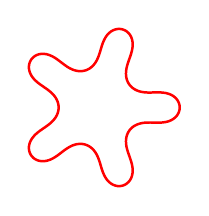
\begin{tikzpicture}[scale=0.45]

  \begin{axis}[
    hide axis,
    axis equal image,
    xmin = -1.42,
    xmax = 1.42,
    ymin = -1.42,
    ymax = 1.42,
    xtick = \empty,
    ytick = \empty,
    title style={align=left},
%    title={\Large $t = 2.99 \times 10^{-2}$ \\ \\ \Large $\nu = 0.38$}
  ]

\addplot[red,line width=2pt] coordinates{
(1.1542e+00,-1.5683e-12)
(1.1521e+00,2.7715e-02)
(1.1455e+00,5.5460e-02)
(1.1342e+00,8.3060e-02)
(1.1178e+00,1.1001e-01)
(1.0958e+00,1.3550e-01)
(1.0683e+00,1.5849e-01)
(1.0358e+00,1.7798e-01)
(9.9887e-01,1.9322e-01)
(9.5866e-01,2.0389e-01)
(9.1618e-01,2.1021e-01)
(8.7237e-01,2.1289e-01)
(8.2802e-01,2.1300e-01)
(7.8370e-01,2.1188e-01)
(7.3992e-01,2.1090e-01)
(6.9718e-01,2.1133e-01)
(6.5612e-01,2.1417e-01)
(6.1746e-01,2.2002e-01)
(5.8201e-01,2.2898e-01)
(5.5047e-01,2.4064e-01)
(5.2334e-01,2.5420e-01)
(5.0081e-01,2.6862e-01)
(4.8274e-01,2.8284e-01)
(4.6868e-01,2.9600e-01)
(4.5795e-01,3.0761e-01)
(4.4962e-01,3.1777e-01)
(4.4254e-01,3.2742e-01)
(4.3553e-01,3.3808e-01)
(4.2794e-01,3.5124e-01)
(4.1981e-01,3.6790e-01)
(4.1176e-01,3.8863e-01)
(4.0468e-01,4.1366e-01)
(3.9964e-01,4.4286e-01)
(3.9760e-01,4.7578e-01)
(3.9926e-01,5.1176e-01)
(4.0486e-01,5.4998e-01)
(4.1418e-01,5.8969e-01)
(4.2649e-01,6.3032e-01)
(4.4073e-01,6.7156e-01)
(4.5554e-01,7.1327e-01)
(4.6949e-01,7.5542e-01)
(4.8111e-01,7.9787e-01)
(4.8909e-01,8.4030e-01)
(4.9239e-01,8.8207e-01)
(4.9039e-01,9.2230e-01)
(4.8297e-01,9.5992e-01)
(4.7051e-01,9.9397e-01)
(4.5380e-01,1.0237e+00)
(4.3380e-01,1.0486e+00)
(4.1143e-01,1.0688e+00)
(3.8735e-01,1.0845e+00)
(3.6191e-01,1.0959e+00)
(3.3516e-01,1.1033e+00)
(3.0704e-01,1.1065e+00)
(2.7755e-01,1.1052e+00)
(2.4697e-01,1.0990e+00)
(2.1593e-01,1.0871e+00)
(1.8536e-01,1.0693e+00)
(1.5633e-01,1.0455e+00)
(1.2983e-01,1.0162e+00)
(1.0657e-01,9.8205e-01)
(8.6754e-02,9.4421e-01)
(7.0115e-02,9.0377e-01)
(5.5924e-02,8.6180e-01)
(4.3149e-02,8.1930e-01)
(3.0636e-02,7.7718e-01)
(1.7298e-02,7.3631e-01)
(2.3040e-03,6.9759e-01)
(-1.4778e-02,6.6193e-01)
(-3.3895e-02,6.3012e-01)
(-5.4525e-02,6.0278e-01)
(-7.5796e-02,5.8022e-01)
(-9.6673e-02,5.6235e-01)
(-1.1616e-01,5.4877e-01)
(-1.3351e-01,5.3883e-01)
(-1.4836e-01,5.3174e-01)
(-1.6095e-01,5.2666e-01)
(-1.7236e-01,5.2276e-01)
(-1.8433e-01,5.1934e-01)
(-1.9858e-01,5.1613e-01)
(-2.1619e-01,5.1339e-01)
(-2.3762e-01,5.1180e-01)
(-2.6288e-01,5.1228e-01)
(-2.9158e-01,5.1579e-01)
(-3.2307e-01,5.2317e-01)
(-3.5650e-01,5.3496e-01)
(-3.9099e-01,5.5123e-01)
(-4.2586e-01,5.7162e-01)
(-4.6072e-01,5.9535e-01)
(-4.9553e-01,6.2132e-01)
(-5.3053e-01,6.4828e-01)
(-5.6614e-01,6.7481e-01)
(-6.0270e-01,6.9952e-01)
(-6.4038e-01,7.2102e-01)
(-6.7896e-01,7.3808e-01)
(-7.1787e-01,7.4976e-01)
(-7.5619e-01,7.5553e-01)
(-7.9288e-01,7.5536e-01)
(-8.2692e-01,7.4966e-01)
(-8.5758e-01,7.3921e-01)
(-8.8447e-01,7.2485e-01)
(-9.0755e-01,7.0735e-01)
(-9.2697e-01,6.8718e-01)
(-9.4291e-01,6.6451e-01)
(-9.5538e-01,6.3929e-01)
(-9.6411e-01,6.1140e-01)
(-9.6854e-01,5.8087e-01)
(-9.6795e-01,5.4807e-01)
(-9.6166e-01,5.1369e-01)
(-9.4925e-01,4.7872e-01)
(-9.3072e-01,4.4424e-01)
(-9.0651e-01,4.1119e-01)
(-8.7748e-01,3.8021e-01)
(-8.4475e-01,3.5146e-01)
(-8.0956e-01,3.2467e-01)
(-7.7318e-01,2.9922e-01)
(-7.3683e-01,2.7429e-01)
(-7.0170e-01,2.4911e-01)
(-6.6892e-01,2.2309e-01)
(-6.3950e-01,1.9602e-01)
(-6.1425e-01,1.6811e-01)
(-5.9367e-01,1.3999e-01)
(-5.7786e-01,1.1254e-01)
(-5.6649e-01,8.6721e-02)
(-5.5894e-01,6.3407e-02)
(-5.5435e-01,4.3180e-02)
(-5.5187e-01,2.6233e-02)
(-5.5074e-01,1.2209e-02)
(-5.5043e-01,1.8275e-12)
(-5.5074e-01,-1.2209e-02)
(-5.5187e-01,-2.6233e-02)
(-5.5435e-01,-4.3180e-02)
(-5.5894e-01,-6.3407e-02)
(-5.6649e-01,-8.6721e-02)
(-5.7786e-01,-1.1254e-01)
(-5.9367e-01,-1.3999e-01)
(-6.1425e-01,-1.6811e-01)
(-6.3950e-01,-1.9602e-01)
(-6.6892e-01,-2.2309e-01)
(-7.0170e-01,-2.4911e-01)
(-7.3683e-01,-2.7429e-01)
(-7.7318e-01,-2.9922e-01)
(-8.0956e-01,-3.2467e-01)
(-8.4475e-01,-3.5146e-01)
(-8.7748e-01,-3.8021e-01)
(-9.0651e-01,-4.1119e-01)
(-9.3072e-01,-4.4424e-01)
(-9.4925e-01,-4.7872e-01)
(-9.6166e-01,-5.1369e-01)
(-9.6795e-01,-5.4807e-01)
(-9.6854e-01,-5.8087e-01)
(-9.6411e-01,-6.1140e-01)
(-9.5538e-01,-6.3929e-01)
(-9.4291e-01,-6.6451e-01)
(-9.2697e-01,-6.8718e-01)
(-9.0755e-01,-7.0735e-01)
(-8.8447e-01,-7.2485e-01)
(-8.5758e-01,-7.3921e-01)
(-8.2692e-01,-7.4966e-01)
(-7.9288e-01,-7.5536e-01)
(-7.5619e-01,-7.5553e-01)
(-7.1787e-01,-7.4976e-01)
(-6.7896e-01,-7.3808e-01)
(-6.4038e-01,-7.2102e-01)
(-6.0270e-01,-6.9952e-01)
(-5.6614e-01,-6.7481e-01)
(-5.3053e-01,-6.4828e-01)
(-4.9553e-01,-6.2132e-01)
(-4.6072e-01,-5.9535e-01)
(-4.2586e-01,-5.7162e-01)
(-3.9099e-01,-5.5123e-01)
(-3.5650e-01,-5.3496e-01)
(-3.2307e-01,-5.2317e-01)
(-2.9158e-01,-5.1579e-01)
(-2.6288e-01,-5.1228e-01)
(-2.3762e-01,-5.1180e-01)
(-2.1619e-01,-5.1339e-01)
(-1.9858e-01,-5.1613e-01)
(-1.8433e-01,-5.1934e-01)
(-1.7236e-01,-5.2276e-01)
(-1.6095e-01,-5.2666e-01)
(-1.4836e-01,-5.3174e-01)
(-1.3351e-01,-5.3883e-01)
(-1.1616e-01,-5.4877e-01)
(-9.6673e-02,-5.6235e-01)
(-7.5796e-02,-5.8022e-01)
(-5.4525e-02,-6.0278e-01)
(-3.3895e-02,-6.3012e-01)
(-1.4778e-02,-6.6193e-01)
(2.3040e-03,-6.9759e-01)
(1.7298e-02,-7.3631e-01)
(3.0636e-02,-7.7718e-01)
(4.3149e-02,-8.1930e-01)
(5.5924e-02,-8.6180e-01)
(7.0115e-02,-9.0377e-01)
(8.6754e-02,-9.4421e-01)
(1.0657e-01,-9.8205e-01)
(1.2983e-01,-1.0162e+00)
(1.5633e-01,-1.0455e+00)
(1.8536e-01,-1.0693e+00)
(2.1593e-01,-1.0871e+00)
(2.4697e-01,-1.0990e+00)
(2.7755e-01,-1.1052e+00)
(3.0704e-01,-1.1065e+00)
(3.3516e-01,-1.1033e+00)
(3.6191e-01,-1.0959e+00)
(3.8735e-01,-1.0845e+00)
(4.1143e-01,-1.0688e+00)
(4.3380e-01,-1.0486e+00)
(4.5380e-01,-1.0237e+00)
(4.7051e-01,-9.9397e-01)
(4.8297e-01,-9.5992e-01)
(4.9039e-01,-9.2230e-01)
(4.9239e-01,-8.8207e-01)
(4.8909e-01,-8.4030e-01)
(4.8111e-01,-7.9787e-01)
(4.6949e-01,-7.5542e-01)
(4.5554e-01,-7.1327e-01)
(4.4073e-01,-6.7156e-01)
(4.2649e-01,-6.3032e-01)
(4.1418e-01,-5.8969e-01)
(4.0486e-01,-5.4998e-01)
(3.9926e-01,-5.1176e-01)
(3.9760e-01,-4.7578e-01)
(3.9964e-01,-4.4286e-01)
(4.0468e-01,-4.1366e-01)
(4.1176e-01,-3.8863e-01)
(4.1981e-01,-3.6790e-01)
(4.2794e-01,-3.5124e-01)
(4.3553e-01,-3.3808e-01)
(4.4254e-01,-3.2742e-01)
(4.4962e-01,-3.1777e-01)
(4.5795e-01,-3.0761e-01)
(4.6868e-01,-2.9600e-01)
(4.8274e-01,-2.8284e-01)
(5.0081e-01,-2.6862e-01)
(5.2334e-01,-2.5420e-01)
(5.5047e-01,-2.4064e-01)
(5.8201e-01,-2.2898e-01)
(6.1746e-01,-2.2002e-01)
(6.5612e-01,-2.1417e-01)
(6.9718e-01,-2.1133e-01)
(7.3992e-01,-2.1090e-01)
(7.8370e-01,-2.1188e-01)
(8.2802e-01,-2.1300e-01)
(8.7237e-01,-2.1289e-01)
(9.1618e-01,-2.1021e-01)
(9.5866e-01,-2.0389e-01)
(9.9887e-01,-1.9322e-01)
(1.0358e+00,-1.7798e-01)
(1.0683e+00,-1.5849e-01)
(1.0958e+00,-1.3550e-01)
(1.1178e+00,-1.1001e-01)
(1.1342e+00,-8.3060e-02)
(1.1455e+00,-5.5460e-02)
(1.1521e+00,-2.7715e-02)
(1.1542e+00,-1.5683e-12)
};


\end{axis}

\end{tikzpicture}

%    \quad
%    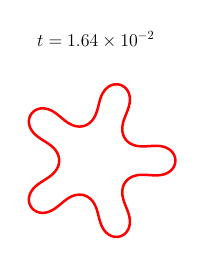
\begin{tikzpicture}[scale=0.45]

  \begin{axis}[
    hide axis,
    axis equal image,
    xmin = -2.1,
    xmax = 2.1,
    ymin = -2.1,
    ymax = 2.1,
    xtick = \empty,
    ytick = \empty,
    title style={align=left},
    title={\Large $t = 1.64 \times 10^{-2}$}
  ]

\addplot[red,line width=2pt] coordinates{
(1.6571e+00,-2.4995e-13)
(1.6540e+00,4.0568e-02)
(1.6446e+00,8.1200e-02)
(1.6282e+00,1.2166e-01)
(1.6043e+00,1.6121e-01)
(1.5722e+00,1.9863e-01)
(1.5321e+00,2.3234e-01)
(1.4844e+00,2.6078e-01)
(1.4303e+00,2.8269e-01)
(1.3712e+00,2.9752e-01)
(1.3088e+00,3.0550e-01)
(1.2447e+00,3.0765e-01)
(1.1798e+00,3.0562e-01)
(1.1150e+00,3.0146e-01)
(1.0511e+00,2.9730e-01)
(9.8855e-01,2.9516e-01)
(9.2832e-01,2.9667e-01)
(8.7143e-01,3.0283e-01)
(8.1907e-01,3.1391e-01)
(7.7235e-01,3.2939e-01)
(7.3210e-01,3.4809e-01)
(6.9865e-01,3.6843e-01)
(6.7184e-01,3.8879e-01)
(6.5103e-01,4.0781e-01)
(6.3518e-01,4.2470e-01)
(6.2292e-01,4.3956e-01)
(6.1255e-01,4.5367e-01)
(6.0232e-01,4.6933e-01)
(5.9132e-01,4.8869e-01)
(5.7970e-01,5.1321e-01)
(5.6840e-01,5.4374e-01)
(5.5884e-01,5.8058e-01)
(5.5264e-01,6.2350e-01)
(5.5125e-01,6.7177e-01)
(5.5567e-01,7.2429e-01)
(5.6620e-01,7.7984e-01)
(5.8238e-01,8.3730e-01)
(6.0302e-01,8.9592e-01)
(6.2643e-01,9.5532e-01)
(6.5053e-01,1.0155e+00)
(6.7308e-01,1.0764e+00)
(6.9187e-01,1.1380e+00)
(7.0491e-01,1.1998e+00)
(7.1065e-01,1.2609e+00)
(7.0821e-01,1.3198e+00)
(6.9750e-01,1.3749e+00)
(6.7921e-01,1.4247e+00)
(6.5461e-01,1.4681e+00)
(6.2519e-01,1.5045e+00)
(5.9232e-01,1.5339e+00)
(5.5701e-01,1.5567e+00)
(5.1976e-01,1.5734e+00)
(4.8061e-01,1.5842e+00)
(4.3946e-01,1.5890e+00)
(3.9629e-01,1.5873e+00)
(3.5151e-01,1.5783e+00)
(3.0601e-01,1.5611e+00)
(2.6120e-01,1.5352e+00)
(2.1875e-01,1.5003e+00)
(1.8023e-01,1.4572e+00)
(1.4679e-01,1.4068e+00)
(1.1886e-01,1.3509e+00)
(9.6059e-02,1.2911e+00)
(7.7305e-02,1.2290e+00)
(6.0987e-02,1.1662e+00)
(4.5272e-02,1.1038e+00)
(2.8403e-02,1.0432e+00)
(8.9895e-03,9.8560e-01)
(-1.3754e-02,9.3237e-01)
(-3.9864e-02,8.8474e-01)
(-6.8632e-02,8.4370e-01)
(-9.8765e-02,8.0976e-01)
(-1.2869e-01,7.8288e-01)
(-1.5685e-01,7.6249e-01)
(-1.8205e-01,7.4761e-01)
(-2.0372e-01,7.3704e-01)
(-2.2214e-01,7.2952e-01)
(-2.3883e-01,7.2379e-01)
(-2.5638e-01,7.1883e-01)
(-2.7730e-01,7.1424e-01)
(-3.0312e-01,7.1049e-01)
(-3.3453e-01,7.0863e-01)
(-3.7147e-01,7.1008e-01)
(-4.1334e-01,7.1633e-01)
(-4.5905e-01,7.2861e-01)
(-5.0730e-01,7.4766e-01)
(-5.5676e-01,7.7353e-01)
(-6.0644e-01,8.0557e-01)
(-6.5587e-01,8.4253e-01)
(-7.0512e-01,8.8272e-01)
(-7.5471e-01,9.2421e-01)
(-8.0539e-01,9.6491e-01)
(-8.5779e-01,1.0027e+00)
(-9.1218e-01,1.0354e+00)
(-9.6824e-01,1.0613e+00)
(-1.0250e+00,1.0789e+00)
(-1.0811e+00,1.0876e+00)
(-1.1348e+00,1.0873e+00)
(-1.1845e+00,1.0788e+00)
(-1.2294e+00,1.0633e+00)
(-1.2686e+00,1.0422e+00)
(-1.3023e+00,1.0164e+00)
(-1.3307e+00,9.8687e-01)
(-1.3541e+00,9.5370e-01)
(-1.3724e+00,9.1682e-01)
(-1.3853e+00,8.7603e-01)
(-1.3920e+00,8.3139e-01)
(-1.3913e+00,7.8337e-01)
(-1.3822e+00,7.3304e-01)
(-1.3640e+00,6.8186e-01)
(-1.3367e+00,6.3152e-01)
(-1.3007e+00,5.8355e-01)
(-1.2574e+00,5.3896e-01)
(-1.2085e+00,4.9808e-01)
(-1.1558e+00,4.6051e-01)
(-1.1012e+00,4.2525e-01)
(-1.0466e+00,3.9099e-01)
(-9.9359e-01,3.5642e-01)
(-9.4396e-01,3.2051e-01)
(-8.9923e-01,2.8279e-01)
(-8.6065e-01,2.4347e-01)
(-8.2907e-01,2.0343e-01)
(-8.0469e-01,1.6398e-01)
(-7.8711e-01,1.2663e-01)
(-7.7539e-01,9.2723e-02)
(-7.6827e-01,6.3215e-02)
(-7.6441e-01,3.8427e-02)
(-7.6264e-01,1.7877e-02)
(-7.6216e-01,-1.0277e-13)
(-7.6264e-01,-1.7877e-02)
(-7.6441e-01,-3.8427e-02)
(-7.6827e-01,-6.3215e-02)
(-7.7539e-01,-9.2723e-02)
(-7.8711e-01,-1.2663e-01)
(-8.0469e-01,-1.6398e-01)
(-8.2907e-01,-2.0343e-01)
(-8.6065e-01,-2.4347e-01)
(-8.9923e-01,-2.8279e-01)
(-9.4396e-01,-3.2051e-01)
(-9.9359e-01,-3.5642e-01)
(-1.0466e+00,-3.9099e-01)
(-1.1012e+00,-4.2525e-01)
(-1.1558e+00,-4.6051e-01)
(-1.2085e+00,-4.9808e-01)
(-1.2574e+00,-5.3896e-01)
(-1.3007e+00,-5.8355e-01)
(-1.3367e+00,-6.3152e-01)
(-1.3640e+00,-6.8186e-01)
(-1.3822e+00,-7.3304e-01)
(-1.3913e+00,-7.8337e-01)
(-1.3920e+00,-8.3139e-01)
(-1.3853e+00,-8.7603e-01)
(-1.3724e+00,-9.1682e-01)
(-1.3541e+00,-9.5370e-01)
(-1.3307e+00,-9.8687e-01)
(-1.3023e+00,-1.0164e+00)
(-1.2686e+00,-1.0422e+00)
(-1.2294e+00,-1.0633e+00)
(-1.1845e+00,-1.0788e+00)
(-1.1348e+00,-1.0873e+00)
(-1.0811e+00,-1.0876e+00)
(-1.0250e+00,-1.0789e+00)
(-9.6824e-01,-1.0613e+00)
(-9.1218e-01,-1.0354e+00)
(-8.5779e-01,-1.0027e+00)
(-8.0539e-01,-9.6491e-01)
(-7.5471e-01,-9.2421e-01)
(-7.0512e-01,-8.8272e-01)
(-6.5587e-01,-8.4253e-01)
(-6.0644e-01,-8.0557e-01)
(-5.5676e-01,-7.7353e-01)
(-5.0730e-01,-7.4766e-01)
(-4.5905e-01,-7.2861e-01)
(-4.1334e-01,-7.1633e-01)
(-3.7147e-01,-7.1008e-01)
(-3.3453e-01,-7.0863e-01)
(-3.0312e-01,-7.1049e-01)
(-2.7730e-01,-7.1424e-01)
(-2.5638e-01,-7.1883e-01)
(-2.3883e-01,-7.2379e-01)
(-2.2214e-01,-7.2952e-01)
(-2.0372e-01,-7.3704e-01)
(-1.8205e-01,-7.4761e-01)
(-1.5685e-01,-7.6249e-01)
(-1.2869e-01,-7.8288e-01)
(-9.8765e-02,-8.0976e-01)
(-6.8632e-02,-8.4370e-01)
(-3.9864e-02,-8.8474e-01)
(-1.3754e-02,-9.3237e-01)
(8.9895e-03,-9.8560e-01)
(2.8403e-02,-1.0432e+00)
(4.5272e-02,-1.1038e+00)
(6.0987e-02,-1.1662e+00)
(7.7305e-02,-1.2290e+00)
(9.6059e-02,-1.2911e+00)
(1.1886e-01,-1.3509e+00)
(1.4679e-01,-1.4068e+00)
(1.8023e-01,-1.4572e+00)
(2.1875e-01,-1.5003e+00)
(2.6120e-01,-1.5352e+00)
(3.0601e-01,-1.5611e+00)
(3.5151e-01,-1.5783e+00)
(3.9629e-01,-1.5873e+00)
(4.3946e-01,-1.5890e+00)
(4.8061e-01,-1.5842e+00)
(5.1976e-01,-1.5734e+00)
(5.5701e-01,-1.5567e+00)
(5.9232e-01,-1.5339e+00)
(6.2519e-01,-1.5045e+00)
(6.5461e-01,-1.4681e+00)
(6.7921e-01,-1.4247e+00)
(6.9750e-01,-1.3749e+00)
(7.0821e-01,-1.3198e+00)
(7.1065e-01,-1.2609e+00)
(7.0491e-01,-1.1998e+00)
(6.9187e-01,-1.1380e+00)
(6.7308e-01,-1.0764e+00)
(6.5053e-01,-1.0155e+00)
(6.2643e-01,-9.5532e-01)
(6.0302e-01,-8.9592e-01)
(5.8238e-01,-8.3730e-01)
(5.6620e-01,-7.7984e-01)
(5.5567e-01,-7.2429e-01)
(5.5125e-01,-6.7177e-01)
(5.5264e-01,-6.2350e-01)
(5.5884e-01,-5.8058e-01)
(5.6840e-01,-5.4374e-01)
(5.7970e-01,-5.1321e-01)
(5.9132e-01,-4.8869e-01)
(6.0232e-01,-4.6933e-01)
(6.1255e-01,-4.5367e-01)
(6.2292e-01,-4.3956e-01)
(6.3518e-01,-4.2470e-01)
(6.5103e-01,-4.0781e-01)
(6.7184e-01,-3.8879e-01)
(6.9865e-01,-3.6843e-01)
(7.3210e-01,-3.4809e-01)
(7.7235e-01,-3.2939e-01)
(8.1907e-01,-3.1391e-01)
(8.7143e-01,-3.0283e-01)
(9.2832e-01,-2.9667e-01)
(9.8855e-01,-2.9516e-01)
(1.0511e+00,-2.9730e-01)
(1.1150e+00,-3.0146e-01)
(1.1798e+00,-3.0562e-01)
(1.2447e+00,-3.0765e-01)
(1.3088e+00,-3.0550e-01)
(1.3712e+00,-2.9752e-01)
(1.4303e+00,-2.8269e-01)
(1.4844e+00,-2.6078e-01)
(1.5321e+00,-2.3234e-01)
(1.5722e+00,-1.9863e-01)
(1.6043e+00,-1.6121e-01)
(1.6282e+00,-1.2166e-01)
(1.6446e+00,-8.1200e-02)
(1.6540e+00,-4.0568e-02)
(1.6571e+00,-2.4995e-13)
};



\end{axis}

\end{tikzpicture}

%    \quad
%    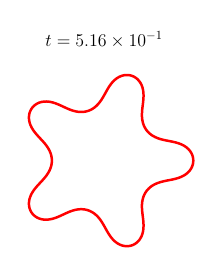
\begin{tikzpicture}[scale=0.45]

  \begin{axis}[
    hide axis,
    axis equal image,
    xmin = -2.1,
    xmax = 2.1,
    ymin = -2.1,
    ymax = 2.1,
    xtick = \empty,
    ytick = \empty,
    title style={align=left},
    title={\Large $t = 5.16 \times 10^{-1}$}
  ]

\addplot[red,line width=2pt] coordinates{
(1.8573e+00,-9.0339e-12)
(1.8547e+00,4.0614e-02)
(1.8468e+00,8.1577e-02)
(1.8329e+00,1.2298e-01)
(1.8125e+00,1.6450e-01)
(1.7849e+00,2.0534e-01)
(1.7499e+00,2.4438e-01)
(1.7076e+00,2.8039e-01)
(1.6587e+00,3.1229e-01)
(1.6042e+00,3.3941e-01)
(1.5454e+00,3.6165e-01)
(1.4837e+00,3.7953e-01)
(1.4204e+00,3.9408e-01)
(1.3568e+00,4.0669e-01)
(1.2938e+00,4.1888e-01)
(1.2327e+00,4.3205e-01)
(1.1744e+00,4.4730e-01)
(1.1200e+00,4.6519e-01)
(1.0706e+00,4.8573e-01)
(1.0269e+00,5.0836e-01)
(9.8935e-01,5.3209e-01)
(9.5812e-01,5.5570e-01)
(9.3291e-01,5.7802e-01)
(9.1310e-01,5.9809e-01)
(8.9780e-01,6.1548e-01)
(8.8578e-01,6.3053e-01)
(8.7542e-01,6.4466e-01)
(8.6500e-01,6.6019e-01)
(8.5345e-01,6.7922e-01)
(8.4067e-01,7.0316e-01)
(8.2726e-01,7.3284e-01)
(8.1423e-01,7.6861e-01)
(8.0279e-01,8.1045e-01)
(7.9411e-01,8.5796e-01)
(7.8906e-01,9.1044e-01)
(7.8804e-01,9.6697e-01)
(7.9086e-01,1.0266e+00)
(7.9675e-01,1.0885e+00)
(8.0444e-01,1.1519e+00)
(8.1229e-01,1.2162e+00)
(8.1853e-01,1.2808e+00)
(8.2145e-01,1.3452e+00)
(8.1957e-01,1.4084e+00)
(8.1186e-01,1.4692e+00)
(7.9790e-01,1.5265e+00)
(7.7786e-01,1.5789e+00)
(7.5249e-01,1.6256e+00)
(7.2287e-01,1.6657e+00)
(6.9018e-01,1.6993e+00)
(6.5541e-01,1.7264e+00)
(6.1917e-01,1.7478e+00)
(5.8162e-01,1.7638e+00)
(5.4255e-01,1.7749e+00)
(5.0156e-01,1.7810e+00)
(4.5835e-01,1.7817e+00)
(4.1296e-01,1.7765e+00)
(3.6585e-01,1.7643e+00)
(3.1792e-01,1.7447e+00)
(2.7038e-01,1.7172e+00)
(2.2445e-01,1.6819e+00)
(1.8119e-01,1.6397e+00)
(1.4119e-01,1.5917e+00)
(1.0450e-01,1.5392e+00)
(7.0641e-02,1.4839e+00)
(3.8719e-02,1.4274e+00)
(7.6439e-03,1.3711e+00)
(-2.3635e-02,1.3165e+00)
(-5.5892e-02,1.2650e+00)
(-8.9454e-02,1.2178e+00)
(-1.2412e-01,1.1760e+00)
(-1.5918e-01,1.1401e+00)
(-1.9361e-01,1.1105e+00)
(-2.2623e-01,1.0870e+00)
(-2.5593e-01,1.0689e+00)
(-2.8193e-01,1.0555e+00)
(-3.0396e-01,1.0457e+00)
(-3.2253e-01,1.0385e+00)
(-3.3924e-01,1.0328e+00)
(-3.5674e-01,1.0277e+00)
(-3.7754e-01,1.0226e+00)
(-4.0318e-01,1.0177e+00)
(-4.3440e-01,1.0138e+00)
(-4.7133e-01,1.0119e+00)
(-5.1365e-01,1.0132e+00)
(-5.6068e-01,1.0187e+00)
(-6.1151e-01,1.0291e+00)
(-6.6515e-01,1.0446e+00)
(-7.2070e-01,1.0648e+00)
(-7.7752e-01,1.0890e+00)
(-8.3526e-01,1.1155e+00)
(-8.9383e-01,1.1429e+00)
(-9.5324e-01,1.1693e+00)
(-1.0134e+00,1.1928e+00)
(-1.0741e+00,1.2116e+00)
(-1.1345e+00,1.2244e+00)
(-1.1936e+00,1.2303e+00)
(-1.2504e+00,1.2289e+00)
(-1.3034e+00,1.2204e+00)
(-1.3518e+00,1.2058e+00)
(-1.3949e+00,1.1860e+00)
(-1.4325e+00,1.1620e+00)
(-1.4650e+00,1.1348e+00)
(-1.4927e+00,1.1046e+00)
(-1.5161e+00,1.0715e+00)
(-1.5355e+00,1.0351e+00)
(-1.5505e+00,9.9499e-01)
(-1.5606e+00,9.5098e-01)
(-1.5649e+00,9.0314e-01)
(-1.5624e+00,8.5203e-01)
(-1.5525e+00,7.9862e-01)
(-1.5347e+00,7.4413e-01)
(-1.5094e+00,6.8978e-01)
(-1.4773e+00,6.3657e-01)
(-1.4397e+00,5.8510e-01)
(-1.3981e+00,5.3547e-01)
(-1.3544e+00,4.8738e-01)
(-1.3103e+00,4.4029e-01)
(-1.2676e+00,3.9364e-01)
(-1.2278e+00,3.4705e-01)
(-1.1923e+00,3.0051e-01)
(-1.1621e+00,2.5444e-01)
(-1.1377e+00,2.0964e-01)
(-1.1191e+00,1.6716e-01)
(-1.1058e+00,1.2807e-01)
(-1.0970e+00,9.3280e-02)
(-1.0917e+00,6.3390e-02)
(-1.0888e+00,3.8466e-02)
(-1.0875e+00,1.7880e-02)
(-1.0871e+00,1.1759e-11)
(-1.0875e+00,-1.7880e-02)
(-1.0888e+00,-3.8466e-02)
(-1.0917e+00,-6.3390e-02)
(-1.0970e+00,-9.3280e-02)
(-1.1058e+00,-1.2807e-01)
(-1.1191e+00,-1.6716e-01)
(-1.1377e+00,-2.0964e-01)
(-1.1621e+00,-2.5444e-01)
(-1.1923e+00,-3.0051e-01)
(-1.2278e+00,-3.4705e-01)
(-1.2676e+00,-3.9364e-01)
(-1.3103e+00,-4.4029e-01)
(-1.3544e+00,-4.8738e-01)
(-1.3981e+00,-5.3547e-01)
(-1.4397e+00,-5.8510e-01)
(-1.4773e+00,-6.3657e-01)
(-1.5094e+00,-6.8978e-01)
(-1.5347e+00,-7.4413e-01)
(-1.5525e+00,-7.9862e-01)
(-1.5624e+00,-8.5203e-01)
(-1.5649e+00,-9.0314e-01)
(-1.5606e+00,-9.5098e-01)
(-1.5505e+00,-9.9499e-01)
(-1.5355e+00,-1.0351e+00)
(-1.5161e+00,-1.0715e+00)
(-1.4927e+00,-1.1046e+00)
(-1.4650e+00,-1.1348e+00)
(-1.4325e+00,-1.1620e+00)
(-1.3949e+00,-1.1860e+00)
(-1.3518e+00,-1.2058e+00)
(-1.3034e+00,-1.2204e+00)
(-1.2504e+00,-1.2289e+00)
(-1.1936e+00,-1.2303e+00)
(-1.1345e+00,-1.2244e+00)
(-1.0741e+00,-1.2116e+00)
(-1.0134e+00,-1.1928e+00)
(-9.5324e-01,-1.1693e+00)
(-8.9383e-01,-1.1429e+00)
(-8.3526e-01,-1.1155e+00)
(-7.7752e-01,-1.0890e+00)
(-7.2070e-01,-1.0648e+00)
(-6.6515e-01,-1.0446e+00)
(-6.1151e-01,-1.0291e+00)
(-5.6068e-01,-1.0187e+00)
(-5.1365e-01,-1.0132e+00)
(-4.7133e-01,-1.0119e+00)
(-4.3440e-01,-1.0138e+00)
(-4.0318e-01,-1.0177e+00)
(-3.7754e-01,-1.0226e+00)
(-3.5674e-01,-1.0277e+00)
(-3.3924e-01,-1.0328e+00)
(-3.2253e-01,-1.0385e+00)
(-3.0396e-01,-1.0457e+00)
(-2.8193e-01,-1.0555e+00)
(-2.5593e-01,-1.0689e+00)
(-2.2623e-01,-1.0870e+00)
(-1.9361e-01,-1.1105e+00)
(-1.5918e-01,-1.1401e+00)
(-1.2412e-01,-1.1760e+00)
(-8.9454e-02,-1.2178e+00)
(-5.5892e-02,-1.2650e+00)
(-2.3635e-02,-1.3165e+00)
(7.6439e-03,-1.3711e+00)
(3.8719e-02,-1.4274e+00)
(7.0641e-02,-1.4839e+00)
(1.0450e-01,-1.5392e+00)
(1.4119e-01,-1.5917e+00)
(1.8119e-01,-1.6397e+00)
(2.2445e-01,-1.6819e+00)
(2.7038e-01,-1.7172e+00)
(3.1792e-01,-1.7447e+00)
(3.6585e-01,-1.7643e+00)
(4.1296e-01,-1.7765e+00)
(4.5835e-01,-1.7817e+00)
(5.0156e-01,-1.7810e+00)
(5.4255e-01,-1.7749e+00)
(5.8162e-01,-1.7638e+00)
(6.1917e-01,-1.7478e+00)
(6.5541e-01,-1.7264e+00)
(6.9018e-01,-1.6993e+00)
(7.2287e-01,-1.6657e+00)
(7.5249e-01,-1.6256e+00)
(7.7786e-01,-1.5789e+00)
(7.9790e-01,-1.5265e+00)
(8.1186e-01,-1.4692e+00)
(8.1957e-01,-1.4084e+00)
(8.2145e-01,-1.3452e+00)
(8.1853e-01,-1.2808e+00)
(8.1229e-01,-1.2162e+00)
(8.0444e-01,-1.1519e+00)
(7.9675e-01,-1.0885e+00)
(7.9086e-01,-1.0266e+00)
(7.8804e-01,-9.6697e-01)
(7.8906e-01,-9.1044e-01)
(7.9411e-01,-8.5796e-01)
(8.0279e-01,-8.1045e-01)
(8.1423e-01,-7.6861e-01)
(8.2726e-01,-7.3284e-01)
(8.4067e-01,-7.0316e-01)
(8.5345e-01,-6.7922e-01)
(8.6500e-01,-6.6019e-01)
(8.7542e-01,-6.4466e-01)
(8.8578e-01,-6.3053e-01)
(8.9780e-01,-6.1548e-01)
(9.1310e-01,-5.9809e-01)
(9.3291e-01,-5.7802e-01)
(9.5812e-01,-5.5570e-01)
(9.8935e-01,-5.3209e-01)
(1.0269e+00,-5.0836e-01)
(1.0706e+00,-4.8573e-01)
(1.1200e+00,-4.6519e-01)
(1.1744e+00,-4.4730e-01)
(1.2327e+00,-4.3205e-01)
(1.2938e+00,-4.1888e-01)
(1.3568e+00,-4.0669e-01)
(1.4204e+00,-3.9408e-01)
(1.4837e+00,-3.7953e-01)
(1.5454e+00,-3.6165e-01)
(1.6042e+00,-3.3941e-01)
(1.6587e+00,-3.1229e-01)
(1.7076e+00,-2.8039e-01)
(1.7499e+00,-2.4438e-01)
(1.7849e+00,-2.0534e-01)
(1.8125e+00,-1.6450e-01)
(1.8329e+00,-1.2298e-01)
(1.8468e+00,-8.1577e-02)
(1.8547e+00,-4.0614e-02)
(1.8573e+00,-9.0339e-12)
};



\end{axis}

\end{tikzpicture}

%    \quad
%    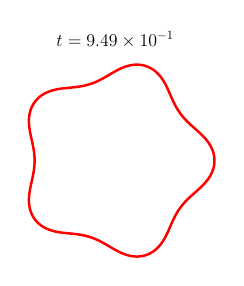
\begin{tikzpicture}[scale=0.45]

  \begin{axis}[
    hide axis,
    axis equal image,
    xmin = -2.1,
    xmax = 2.1,
    ymin = -2.1,
    ymax = 2.1,
    xtick = \empty,
    ytick = \empty,
    title style={align=left},
    title={\Large $t = 9.49 \times 10^{-1}$}
  ]

\addplot[red,line width=2pt] coordinates{
(2.0699e+00,-5.6473e-11)
(2.0685e+00,4.0691e-02)
(2.0641e+00,8.2211e-02)
(2.0564e+00,1.2521e-01)
(2.0450e+00,1.7005e-01)
(2.0292e+00,2.1674e-01)
(2.0085e+00,2.6499e-01)
(1.9828e+00,3.1424e-01)
(1.9519e+00,3.6386e-01)
(1.9161e+00,4.1317e-01)
(1.8760e+00,4.6160e-01)
(1.8324e+00,5.0875e-01)
(1.7863e+00,5.5443e-01)
(1.7387e+00,5.9859e-01)
(1.6909e+00,6.4131e-01)
(1.6440e+00,6.8270e-01)
(1.5990e+00,7.2276e-01)
(1.5568e+00,7.6141e-01)
(1.5181e+00,7.9839e-01)
(1.4833e+00,8.3329e-01)
(1.4529e+00,8.6561e-01)
(1.4268e+00,8.9485e-01)
(1.4051e+00,9.2056e-01)
(1.3873e+00,9.4249e-01)
(1.3731e+00,9.6079e-01)
(1.3616e+00,9.7620e-01)
(1.3513e+00,9.9036e-01)
(1.3405e+00,1.0056e+00)
(1.3279e+00,1.0240e+00)
(1.3130e+00,1.0467e+00)
(1.2957e+00,1.0743e+00)
(1.2763e+00,1.1071e+00)
(1.2553e+00,1.1450e+00)
(1.2330e+00,1.1879e+00)
(1.2099e+00,1.2353e+00)
(1.1863e+00,1.2867e+00)
(1.1622e+00,1.3413e+00)
(1.1375e+00,1.3984e+00)
(1.1119e+00,1.4568e+00)
(1.0849e+00,1.5157e+00)
(1.0561e+00,1.5740e+00)
(1.0252e+00,1.6305e+00)
(9.9198e-01,1.6843e+00)
(9.5655e-01,1.7344e+00)
(9.1923e-01,1.7800e+00)
(8.8054e-01,1.8208e+00)
(8.4111e-01,1.8563e+00)
(8.0155e-01,1.8868e+00)
(7.6235e-01,1.9125e+00)
(7.2371e-01,1.9338e+00)
(6.8552e-01,1.9515e+00)
(6.4734e-01,1.9660e+00)
(6.0845e-01,1.9777e+00)
(5.6801e-01,1.9869e+00)
(5.2528e-01,1.9935e+00)
(4.7970e-01,1.9971e+00)
(4.3103e-01,1.9972e+00)
(3.7934e-01,1.9934e+00)
(3.2500e-01,1.9851e+00)
(2.6860e-01,1.9720e+00)
(2.1083e-01,1.9542e+00)
(1.5243e-01,1.9318e+00)
(9.4027e-02,1.9056e+00)
(3.6168e-02,1.8763e+00)
(-2.0752e-02,1.8450e+00)
(-7.6433e-02,1.8129e+00)
(-1.3062e-01,1.7809e+00)
(-1.8303e-01,1.7501e+00)
(-2.3332e-01,1.7214e+00)
(-2.8103e-01,1.6954e+00)
(-3.2564e-01,1.6725e+00)
(-3.6659e-01,1.6529e+00)
(-4.0334e-01,1.6365e+00)
(-4.3548e-01,1.6232e+00)
(-4.6277e-01,1.6126e+00)
(-4.8543e-01,1.6043e+00)
(-5.0424e-01,1.5978e+00)
(-5.2100e-01,1.5923e+00)
(-5.3840e-01,1.5868e+00)
(-5.5893e-01,1.5807e+00)
(-5.8408e-01,1.5737e+00)
(-6.1457e-01,1.5660e+00)
(-6.5062e-01,1.5577e+00)
(-6.9215e-01,1.5494e+00)
(-7.3882e-01,1.5413e+00)
(-7.9018e-01,1.5339e+00)
(-8.4562e-01,1.5272e+00)
(-9.0443e-01,1.5210e+00)
(-9.6588e-01,1.5152e+00)
(-1.0291e+00,1.5090e+00)
(-1.0934e+00,1.5018e+00)
(-1.1578e+00,1.4929e+00)
(-1.2214e+00,1.4815e+00)
(-1.2832e+00,1.4672e+00)
(-1.3424e+00,1.4496e+00)
(-1.3982e+00,1.4288e+00)
(-1.4498e+00,1.4051e+00)
(-1.4967e+00,1.3790e+00)
(-1.5389e+00,1.3511e+00)
(-1.5763e+00,1.3219e+00)
(-1.6094e+00,1.2919e+00)
(-1.6387e+00,1.2612e+00)
(-1.6648e+00,1.2296e+00)
(-1.6884e+00,1.1966e+00)
(-1.7100e+00,1.1615e+00)
(-1.7298e+00,1.1236e+00)
(-1.7478e+00,1.0821e+00)
(-1.7635e+00,1.0367e+00)
(-1.7764e+00,9.8714e-01)
(-1.7860e+00,9.3364e-01)
(-1.7918e+00,8.7660e-01)
(-1.7935e+00,8.1664e-01)
(-1.7911e+00,7.5452e-01)
(-1.7849e+00,6.9105e-01)
(-1.7755e+00,6.2701e-01)
(-1.7637e+00,5.6310e-01)
(-1.7505e+00,4.9997e-01)
(-1.7368e+00,4.3821e-01)
(-1.7236e+00,3.7839e-01)
(-1.7115e+00,3.2111e-01)
(-1.7011e+00,2.6699e-01)
(-1.6927e+00,2.1666e-01)
(-1.6863e+00,1.7071e-01)
(-1.6818e+00,1.2966e-01)
(-1.6788e+00,9.3894e-02)
(-1.6770e+00,6.3583e-02)
(-1.6760e+00,3.8509e-02)
(-1.6755e+00,1.7885e-02)
(-1.6754e+00,-9.7486e-12)
(-1.6755e+00,-1.7885e-02)
(-1.6760e+00,-3.8509e-02)
(-1.6770e+00,-6.3583e-02)
(-1.6788e+00,-9.3894e-02)
(-1.6818e+00,-1.2966e-01)
(-1.6863e+00,-1.7071e-01)
(-1.6927e+00,-2.1666e-01)
(-1.7011e+00,-2.6699e-01)
(-1.7115e+00,-3.2111e-01)
(-1.7236e+00,-3.7839e-01)
(-1.7368e+00,-4.3821e-01)
(-1.7505e+00,-4.9997e-01)
(-1.7637e+00,-5.6310e-01)
(-1.7755e+00,-6.2701e-01)
(-1.7849e+00,-6.9105e-01)
(-1.7911e+00,-7.5452e-01)
(-1.7935e+00,-8.1664e-01)
(-1.7918e+00,-8.7660e-01)
(-1.7860e+00,-9.3364e-01)
(-1.7764e+00,-9.8714e-01)
(-1.7635e+00,-1.0367e+00)
(-1.7478e+00,-1.0821e+00)
(-1.7298e+00,-1.1236e+00)
(-1.7100e+00,-1.1615e+00)
(-1.6884e+00,-1.1966e+00)
(-1.6648e+00,-1.2296e+00)
(-1.6387e+00,-1.2612e+00)
(-1.6094e+00,-1.2919e+00)
(-1.5763e+00,-1.3219e+00)
(-1.5389e+00,-1.3511e+00)
(-1.4967e+00,-1.3790e+00)
(-1.4498e+00,-1.4051e+00)
(-1.3982e+00,-1.4288e+00)
(-1.3424e+00,-1.4496e+00)
(-1.2832e+00,-1.4672e+00)
(-1.2214e+00,-1.4815e+00)
(-1.1578e+00,-1.4929e+00)
(-1.0934e+00,-1.5018e+00)
(-1.0291e+00,-1.5090e+00)
(-9.6588e-01,-1.5152e+00)
(-9.0443e-01,-1.5210e+00)
(-8.4562e-01,-1.5272e+00)
(-7.9018e-01,-1.5339e+00)
(-7.3882e-01,-1.5413e+00)
(-6.9215e-01,-1.5494e+00)
(-6.5062e-01,-1.5577e+00)
(-6.1457e-01,-1.5660e+00)
(-5.8408e-01,-1.5737e+00)
(-5.5893e-01,-1.5807e+00)
(-5.3840e-01,-1.5868e+00)
(-5.2100e-01,-1.5923e+00)
(-5.0424e-01,-1.5978e+00)
(-4.8543e-01,-1.6043e+00)
(-4.6277e-01,-1.6126e+00)
(-4.3548e-01,-1.6232e+00)
(-4.0334e-01,-1.6365e+00)
(-3.6659e-01,-1.6529e+00)
(-3.2564e-01,-1.6725e+00)
(-2.8103e-01,-1.6954e+00)
(-2.3332e-01,-1.7214e+00)
(-1.8303e-01,-1.7501e+00)
(-1.3062e-01,-1.7809e+00)
(-7.6433e-02,-1.8129e+00)
(-2.0752e-02,-1.8450e+00)
(3.6168e-02,-1.8763e+00)
(9.4027e-02,-1.9056e+00)
(1.5243e-01,-1.9318e+00)
(2.1083e-01,-1.9542e+00)
(2.6860e-01,-1.9720e+00)
(3.2500e-01,-1.9851e+00)
(3.7934e-01,-1.9934e+00)
(4.3103e-01,-1.9972e+00)
(4.7970e-01,-1.9971e+00)
(5.2528e-01,-1.9935e+00)
(5.6801e-01,-1.9869e+00)
(6.0845e-01,-1.9777e+00)
(6.4734e-01,-1.9660e+00)
(6.8552e-01,-1.9515e+00)
(7.2371e-01,-1.9338e+00)
(7.6235e-01,-1.9125e+00)
(8.0155e-01,-1.8868e+00)
(8.4111e-01,-1.8563e+00)
(8.8054e-01,-1.8208e+00)
(9.1923e-01,-1.7800e+00)
(9.5655e-01,-1.7344e+00)
(9.9198e-01,-1.6843e+00)
(1.0252e+00,-1.6305e+00)
(1.0561e+00,-1.5740e+00)
(1.0849e+00,-1.5157e+00)
(1.1119e+00,-1.4568e+00)
(1.1375e+00,-1.3984e+00)
(1.1622e+00,-1.3413e+00)
(1.1863e+00,-1.2867e+00)
(1.2099e+00,-1.2353e+00)
(1.2330e+00,-1.1879e+00)
(1.2553e+00,-1.1450e+00)
(1.2763e+00,-1.1071e+00)
(1.2957e+00,-1.0743e+00)
(1.3130e+00,-1.0467e+00)
(1.3279e+00,-1.0240e+00)
(1.3405e+00,-1.0056e+00)
(1.3513e+00,-9.9036e-01)
(1.3616e+00,-9.7620e-01)
(1.3731e+00,-9.6079e-01)
(1.3873e+00,-9.4249e-01)
(1.4051e+00,-9.2056e-01)
(1.4268e+00,-8.9485e-01)
(1.4529e+00,-8.6561e-01)
(1.4833e+00,-8.3329e-01)
(1.5181e+00,-7.9839e-01)
(1.5568e+00,-7.6141e-01)
(1.5990e+00,-7.2276e-01)
(1.6440e+00,-6.8270e-01)
(1.6909e+00,-6.4131e-01)
(1.7387e+00,-5.9859e-01)
(1.7863e+00,-5.5443e-01)
(1.8324e+00,-5.0875e-01)
(1.8760e+00,-4.6160e-01)
(1.9161e+00,-4.1317e-01)
(1.9519e+00,-3.6386e-01)
(1.9828e+00,-3.1424e-01)
(2.0085e+00,-2.6499e-01)
(2.0292e+00,-2.1674e-01)
(2.0450e+00,-1.7005e-01)
(2.0564e+00,-1.2521e-01)
(2.0641e+00,-8.2211e-02)
(2.0685e+00,-4.0691e-02)
(2.0699e+00,-5.6473e-11)
};


\end{axis}

\end{tikzpicture}

%    \quad
%    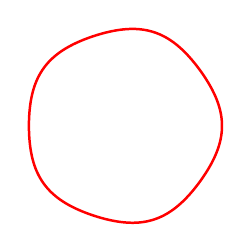
\begin{tikzpicture}[scale=0.45]

  \begin{axis}[
    hide axis,
    axis equal image,
    xmin = -1.42,
    xmax = 1.42,
    ymin = -1.42,
    ymax = 1.42,
    xtick = \empty,
    ytick = \empty,
    title style={align=left},
%    title={\Large $t = 3.17 \times 10^{-1}$ \\ \\ \Large $\nu = 0.99$}
  ]

\addplot[red,line width=2pt] coordinates{
(1.3864e+00,-4.3575e-10)
(1.3860e+00,2.7820e-02)
(1.3847e+00,5.6320e-02)
(1.3823e+00,8.6084e-02)
(1.3788e+00,1.1752e-01)
(1.3739e+00,1.5087e-01)
(1.3674e+00,1.8615e-01)
(1.3591e+00,2.2325e-01)
(1.3488e+00,2.6191e-01)
(1.3367e+00,3.0178e-01)
(1.3226e+00,3.4244e-01)
(1.3068e+00,3.8343e-01)
(1.2894e+00,4.2430e-01)
(1.2707e+00,4.6458e-01)
(1.2512e+00,5.0382e-01)
(1.2311e+00,5.4160e-01)
(1.2109e+00,5.7754e-01)
(1.1911e+00,6.1127e-01)
(1.1719e+00,6.4247e-01)
(1.1539e+00,6.7088e-01)
(1.1372e+00,6.9627e-01)
(1.1223e+00,7.1848e-01)
(1.1093e+00,7.3745e-01)
(1.0982e+00,7.5324e-01)
(1.0891e+00,7.6613e-01)
(1.0814e+00,7.7680e-01)
(1.0744e+00,7.8649e-01)
(1.0668e+00,7.9678e-01)
(1.0578e+00,8.0899e-01)
(1.0466e+00,8.2380e-01)
(1.0331e+00,8.4148e-01)
(1.0171e+00,8.6199e-01)
(9.9861e-01,8.8515e-01)
(9.7765e-01,9.1067e-01)
(9.5434e-01,9.3817e-01)
(9.2882e-01,9.6722e-01)
(9.0126e-01,9.9735e-01)
(8.7187e-01,1.0281e+00)
(8.4088e-01,1.0588e+00)
(8.0857e-01,1.0892e+00)
(7.7524e-01,1.1186e+00)
(7.4124e-01,1.1467e+00)
(7.0693e-01,1.1730e+00)
(6.7270e-01,1.1973e+00)
(6.3895e-01,1.2194e+00)
(6.0603e-01,1.2392e+00)
(5.7424e-01,1.2568e+00)
(5.4378e-01,1.2722e+00)
(5.1469e-01,1.2856e+00)
(4.8689e-01,1.2973e+00)
(4.6005e-01,1.3077e+00)
(4.3370e-01,1.3169e+00)
(4.0721e-01,1.3252e+00)
(3.7993e-01,1.3329e+00)
(3.5125e-01,1.3399e+00)
(3.2068e-01,1.3464e+00)
(2.8790e-01,1.3522e+00)
(2.5280e-01,1.3571e+00)
(2.1539e-01,1.3609e+00)
(1.7586e-01,1.3634e+00)
(1.3451e-01,1.3645e+00)
(9.1724e-02,1.3640e+00)
(4.7970e-02,1.3619e+00)
(3.7546e-03,1.3583e+00)
(-4.0394e-02,1.3532e+00)
(-8.3942e-02,1.3470e+00)
(-1.2636e-01,1.3397e+00)
(-1.6716e-01,1.3318e+00)
(-2.0585e-01,1.3234e+00)
(-2.4200e-01,1.3148e+00)
(-2.7522e-01,1.3064e+00)
(-3.0519e-01,1.2983e+00)
(-3.3165e-01,1.2908e+00)
(-3.5445e-01,1.2841e+00)
(-3.7359e-01,1.2783e+00)
(-3.8931e-01,1.2734e+00)
(-4.0225e-01,1.2693e+00)
(-4.1371e-01,1.2656e+00)
(-4.2554e-01,1.2617e+00)
(-4.3940e-01,1.2571e+00)
(-4.5627e-01,1.2513e+00)
(-4.7656e-01,1.2442e+00)
(-5.0033e-01,1.2356e+00)
(-5.2744e-01,1.2255e+00)
(-5.5761e-01,1.2137e+00)
(-5.9048e-01,1.2004e+00)
(-6.2561e-01,1.1854e+00)
(-6.6249e-01,1.1689e+00)
(-7.0061e-01,1.1507e+00)
(-7.3939e-01,1.1310e+00)
(-7.7827e-01,1.1099e+00)
(-8.1670e-01,1.0876e+00)
(-8.5415e-01,1.0641e+00)
(-8.9013e-01,1.0398e+00)
(-9.2424e-01,1.0148e+00)
(-9.5617e-01,9.8955e-01)
(-9.8569e-01,9.6433e-01)
(-1.0127e+00,9.3942e-01)
(-1.0373e+00,9.1507e-01)
(-1.0595e+00,8.9142e-01)
(-1.0796e+00,8.6848e-01)
(-1.0980e+00,8.4607e-01)
(-1.1151e+00,8.2386e-01)
(-1.1313e+00,8.0137e-01)
(-1.1471e+00,7.7803e-01)
(-1.1627e+00,7.5329e-01)
(-1.1783e+00,7.2664e-01)
(-1.1939e+00,6.9774e-01)
(-1.2095e+00,6.6637e-01)
(-1.2247e+00,6.3247e-01)
(-1.2395e+00,5.9612e-01)
(-1.2535e+00,5.5754e-01)
(-1.2664e+00,5.1703e-01)
(-1.2782e+00,4.7502e-01)
(-1.2887e+00,4.3199e-01)
(-1.2978e+00,3.8847e-01)
(-1.3056e+00,3.4504e-01)
(-1.3121e+00,3.0225e-01)
(-1.3173e+00,2.6068e-01)
(-1.3215e+00,2.2087e-01)
(-1.3247e+00,1.8334e-01)
(-1.3271e+00,1.4853e-01)
(-1.3288e+00,1.1687e-01)
(-1.3299e+00,8.8668e-02)
(-1.3307e+00,6.4158e-02)
(-1.3311e+00,4.3415e-02)
(-1.3314e+00,2.6286e-02)
(-1.3315e+00,1.2214e-02)
(-1.3315e+00,2.3306e-10)
(-1.3315e+00,-1.2214e-02)
(-1.3314e+00,-2.6286e-02)
(-1.3311e+00,-4.3415e-02)
(-1.3307e+00,-6.4158e-02)
(-1.3299e+00,-8.8668e-02)
(-1.3288e+00,-1.1687e-01)
(-1.3271e+00,-1.4853e-01)
(-1.3247e+00,-1.8334e-01)
(-1.3215e+00,-2.2087e-01)
(-1.3173e+00,-2.6068e-01)
(-1.3121e+00,-3.0225e-01)
(-1.3056e+00,-3.4504e-01)
(-1.2978e+00,-3.8847e-01)
(-1.2887e+00,-4.3199e-01)
(-1.2782e+00,-4.7502e-01)
(-1.2664e+00,-5.1703e-01)
(-1.2535e+00,-5.5754e-01)
(-1.2395e+00,-5.9612e-01)
(-1.2247e+00,-6.3247e-01)
(-1.2095e+00,-6.6637e-01)
(-1.1939e+00,-6.9774e-01)
(-1.1783e+00,-7.2664e-01)
(-1.1627e+00,-7.5329e-01)
(-1.1471e+00,-7.7803e-01)
(-1.1313e+00,-8.0137e-01)
(-1.1151e+00,-8.2386e-01)
(-1.0980e+00,-8.4607e-01)
(-1.0796e+00,-8.6848e-01)
(-1.0595e+00,-8.9142e-01)
(-1.0373e+00,-9.1507e-01)
(-1.0127e+00,-9.3942e-01)
(-9.8569e-01,-9.6433e-01)
(-9.5617e-01,-9.8955e-01)
(-9.2424e-01,-1.0148e+00)
(-8.9013e-01,-1.0398e+00)
(-8.5415e-01,-1.0641e+00)
(-8.1670e-01,-1.0876e+00)
(-7.7827e-01,-1.1099e+00)
(-7.3939e-01,-1.1310e+00)
(-7.0061e-01,-1.1507e+00)
(-6.6249e-01,-1.1689e+00)
(-6.2561e-01,-1.1854e+00)
(-5.9048e-01,-1.2004e+00)
(-5.5761e-01,-1.2137e+00)
(-5.2744e-01,-1.2255e+00)
(-5.0033e-01,-1.2356e+00)
(-4.7656e-01,-1.2442e+00)
(-4.5627e-01,-1.2513e+00)
(-4.3940e-01,-1.2571e+00)
(-4.2554e-01,-1.2617e+00)
(-4.1371e-01,-1.2656e+00)
(-4.0225e-01,-1.2693e+00)
(-3.8931e-01,-1.2734e+00)
(-3.7359e-01,-1.2783e+00)
(-3.5445e-01,-1.2841e+00)
(-3.3165e-01,-1.2908e+00)
(-3.0519e-01,-1.2983e+00)
(-2.7522e-01,-1.3064e+00)
(-2.4200e-01,-1.3148e+00)
(-2.0585e-01,-1.3234e+00)
(-1.6716e-01,-1.3318e+00)
(-1.2636e-01,-1.3397e+00)
(-8.3942e-02,-1.3470e+00)
(-4.0394e-02,-1.3532e+00)
(3.7546e-03,-1.3583e+00)
(4.7970e-02,-1.3619e+00)
(9.1724e-02,-1.3640e+00)
(1.3451e-01,-1.3645e+00)
(1.7586e-01,-1.3634e+00)
(2.1539e-01,-1.3609e+00)
(2.5280e-01,-1.3571e+00)
(2.8790e-01,-1.3522e+00)
(3.2068e-01,-1.3464e+00)
(3.5125e-01,-1.3399e+00)
(3.7993e-01,-1.3329e+00)
(4.0721e-01,-1.3252e+00)
(4.3370e-01,-1.3169e+00)
(4.6005e-01,-1.3077e+00)
(4.8689e-01,-1.2973e+00)
(5.1469e-01,-1.2856e+00)
(5.4378e-01,-1.2722e+00)
(5.7424e-01,-1.2568e+00)
(6.0603e-01,-1.2392e+00)
(6.3895e-01,-1.2194e+00)
(6.7270e-01,-1.1973e+00)
(7.0693e-01,-1.1730e+00)
(7.4124e-01,-1.1467e+00)
(7.7524e-01,-1.1186e+00)
(8.0857e-01,-1.0892e+00)
(8.4088e-01,-1.0588e+00)
(8.7187e-01,-1.0281e+00)
(9.0126e-01,-9.9735e-01)
(9.2882e-01,-9.6722e-01)
(9.5434e-01,-9.3817e-01)
(9.7765e-01,-9.1067e-01)
(9.9861e-01,-8.8515e-01)
(1.0171e+00,-8.6199e-01)
(1.0331e+00,-8.4148e-01)
(1.0466e+00,-8.2380e-01)
(1.0578e+00,-8.0899e-01)
(1.0668e+00,-7.9678e-01)
(1.0744e+00,-7.8649e-01)
(1.0814e+00,-7.7680e-01)
(1.0891e+00,-7.6613e-01)
(1.0982e+00,-7.5324e-01)
(1.1093e+00,-7.3745e-01)
(1.1223e+00,-7.1848e-01)
(1.1372e+00,-6.9627e-01)
(1.1539e+00,-6.7088e-01)
(1.1719e+00,-6.4247e-01)
(1.1911e+00,-6.1127e-01)
(1.2109e+00,-5.7754e-01)
(1.2311e+00,-5.4160e-01)
(1.2512e+00,-5.0382e-01)
(1.2707e+00,-4.6458e-01)
(1.2894e+00,-4.2430e-01)
(1.3068e+00,-3.8343e-01)
(1.3226e+00,-3.4244e-01)
(1.3367e+00,-3.0178e-01)
(1.3488e+00,-2.6191e-01)
(1.3591e+00,-2.2325e-01)
(1.3674e+00,-1.8615e-01)
(1.3739e+00,-1.5087e-01)
(1.3788e+00,-1.1752e-01)
(1.3823e+00,-8.6084e-02)
(1.3847e+00,-5.6320e-02)
(1.3860e+00,-2.7820e-02)
(1.3864e+00,-4.3575e-10)
};



\end{axis}

\end{tikzpicture}

%    \fi
%  \caption{\label{fig:starShape} An initially star-shaped semi-permeable
%  vesicle in a quiescent flow with $\beta=1$. Note that the time steps
%  are not equispaced.}
%\end{figure}
%\begin{figure}[htp]
%  \centering
%%  \ifTikz
%  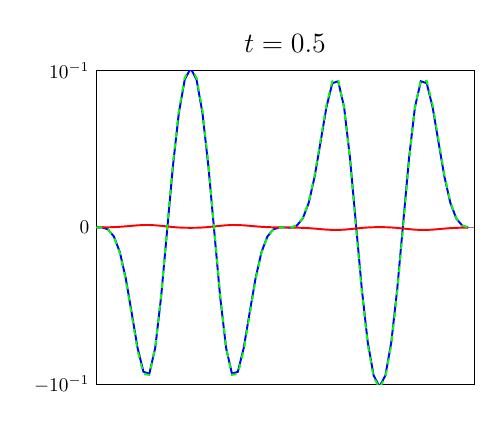
\begin{tikzpicture}[scale=0.7]

\begin{axis}[
    xtick = \empty,
    xmin = 0,
    xmax = 6.2832,
    ymin = -0.1,
    ymax = +0.1,
    ytick = {-0.1,0,0.1},
    yticklabels = {$-10^{-1}$,$0$,$10^{-1}$},
    scaled y ticks = false,
    scaled y ticks = false,
    title = {\Large $t = 0.5$},
  ]

\addplot[blue, line width=1pt] coordinates{
(0.0000e+00,6.0582e-12)
(9.8175e-02,6.4493e-05)
(1.9635e-01,-1.2452e-03)
(2.9452e-01,-5.7788e-03)
(3.9270e-01,-1.5693e-02)
(4.9087e-01,-3.2280e-02)
(5.8905e-01,-5.4213e-02)
(6.8722e-01,-7.6587e-02)
(7.8540e-01,-9.1961e-02)
(8.8357e-01,-9.3196e-02)
(9.8175e-01,-7.6651e-02)
(1.0799e+00,-4.4122e-02)
(1.1781e+00,-2.4484e-03)
(1.2763e+00,3.9226e-02)
(1.3744e+00,7.2989e-02)
(1.4726e+00,9.4253e-02)
(1.5708e+00,1.0142e-01)
(1.6690e+00,9.4253e-02)
(1.7671e+00,7.2989e-02)
(1.8653e+00,3.9226e-02)
(1.9635e+00,-2.4484e-03)
(2.0617e+00,-4.4122e-02)
(2.1598e+00,-7.6651e-02)
(2.2580e+00,-9.3196e-02)
(2.3562e+00,-9.1961e-02)
(2.4544e+00,-7.6587e-02)
(2.5525e+00,-5.4213e-02)
(2.6507e+00,-3.2280e-02)
(2.7489e+00,-1.5693e-02)
(2.8471e+00,-5.7788e-03)
(2.9452e+00,-1.2452e-03)
(3.0434e+00,6.4493e-05)
(3.1416e+00,6.6748e-12)
(3.2398e+00,-6.4493e-05)
(3.3379e+00,1.2452e-03)
(3.4361e+00,5.7788e-03)
(3.5343e+00,1.5693e-02)
(3.6325e+00,3.2280e-02)
(3.7306e+00,5.4213e-02)
(3.8288e+00,7.6587e-02)
(3.9270e+00,9.1961e-02)
(4.0252e+00,9.3196e-02)
(4.1233e+00,7.6651e-02)
(4.2215e+00,4.4122e-02)
(4.3197e+00,2.4484e-03)
(4.4179e+00,-3.9226e-02)
(4.5160e+00,-7.2989e-02)
(4.6142e+00,-9.4253e-02)
(4.7124e+00,-1.0142e-01)
(4.8106e+00,-9.4253e-02)
(4.9087e+00,-7.2989e-02)
(5.0069e+00,-3.9226e-02)
(5.1051e+00,2.4484e-03)
(5.2033e+00,4.4122e-02)
(5.3014e+00,7.6651e-02)
(5.3996e+00,9.3196e-02)
(5.4978e+00,9.1961e-02)
(5.5960e+00,7.6587e-02)
(5.6941e+00,5.4213e-02)
(5.7923e+00,3.2280e-02)
(5.8905e+00,1.5693e-02)
(5.9887e+00,5.7788e-03)
(6.0868e+00,1.2452e-03)
(6.1850e+00,-6.4493e-05)
};

\addplot[red, line width=1pt] coordinates{
(0.0000e+00,6.7339e-18)
(9.8175e-02,4.3333e-05)
(1.9635e-01,1.1058e-04)
(2.9452e-01,2.3031e-04)
(3.9270e-01,4.2984e-04)
(4.9087e-01,7.1540e-04)
(5.8905e-01,1.0514e-03)
(6.8722e-01,1.3614e-03)
(7.8540e-01,1.5567e-03)
(8.8357e-01,1.5722e-03)
(9.8175e-01,1.3903e-03)
(1.0799e+00,1.0511e-03)
(1.1781e+00,6.4307e-04)
(1.2763e+00,2.6721e-04)
(1.3744e+00,-7.6823e-06)
(1.4726e+00,-1.6322e-04)
(1.5708e+00,-2.1189e-04)
(1.6690e+00,-1.6322e-04)
(1.7671e+00,-7.6823e-06)
(1.8653e+00,2.6721e-04)
(1.9635e+00,6.4307e-04)
(2.0617e+00,1.0511e-03)
(2.1598e+00,1.3903e-03)
(2.2580e+00,1.5722e-03)
(2.3562e+00,1.5567e-03)
(2.4544e+00,1.3614e-03)
(2.5525e+00,1.0514e-03)
(2.6507e+00,7.1540e-04)
(2.7489e+00,4.2984e-04)
(2.8471e+00,2.3031e-04)
(2.9452e+00,1.1058e-04)
(3.0434e+00,4.3333e-05)
(3.1416e+00,-2.9592e-17)
(3.2398e+00,-4.3333e-05)
(3.3379e+00,-1.1058e-04)
(3.4361e+00,-2.3031e-04)
(3.5343e+00,-4.2984e-04)
(3.6325e+00,-7.1540e-04)
(3.7306e+00,-1.0514e-03)
(3.8288e+00,-1.3614e-03)
(3.9270e+00,-1.5567e-03)
(4.0252e+00,-1.5722e-03)
(4.1233e+00,-1.3903e-03)
(4.2215e+00,-1.0511e-03)
(4.3197e+00,-6.4307e-04)
(4.4179e+00,-2.6721e-04)
(4.5160e+00,7.6823e-06)
(4.6142e+00,1.6322e-04)
(4.7124e+00,2.1189e-04)
(4.8106e+00,1.6322e-04)
(4.9087e+00,7.6823e-06)
(5.0069e+00,-2.6721e-04)
(5.1051e+00,-6.4307e-04)
(5.2033e+00,-1.0511e-03)
(5.3014e+00,-1.3903e-03)
(5.3996e+00,-1.5722e-03)
(5.4978e+00,-1.5567e-03)
(5.5960e+00,-1.3614e-03)
(5.6941e+00,-1.0514e-03)
(5.7923e+00,-7.1540e-04)
(5.8905e+00,-4.2984e-04)
(5.9887e+00,-2.3031e-04)
(6.0868e+00,-1.1058e-04)
(6.1850e+00,-4.3333e-05)
};

\addplot[green, dashed, line width=1pt] coordinates{
(0.0000e+00,-3.9124e-12)
(9.8175e-02,2.0720e-05)
(1.9635e-01,-1.3715e-03)
(2.9452e-01,-6.0708e-03)
(3.9270e-01,-1.6268e-02)
(4.9087e-01,-3.3236e-02)
(5.8905e-01,-5.5539e-02)
(6.8722e-01,-7.8093e-02)
(7.8540e-01,-9.3289e-02)
(8.8357e-01,-9.3941e-02)
(9.8175e-01,-7.6532e-02)
(1.0799e+00,-4.3130e-02)
(1.1781e+00,-8.7651e-04)
(1.2763e+00,4.0917e-02)
(1.3744e+00,7.4420e-02)
(1.4726e+00,9.5324e-02)
(1.5708e+00,1.0233e-01)
(1.6690e+00,9.5324e-02)
(1.7671e+00,7.4420e-02)
(1.8653e+00,4.0917e-02)
(1.9635e+00,-8.7651e-04)
(2.0617e+00,-4.3130e-02)
(2.1598e+00,-7.6532e-02)
(2.2580e+00,-9.3941e-02)
(2.3562e+00,-9.3289e-02)
(2.4544e+00,-7.8093e-02)
(2.5525e+00,-5.5539e-02)
(2.6507e+00,-3.3236e-02)
(2.7489e+00,-1.6268e-02)
(2.8471e+00,-6.0708e-03)
(2.9452e+00,-1.3715e-03)
(3.0434e+00,2.0720e-05)
(3.1416e+00,5.6502e-13)
(3.2398e+00,-2.0720e-05)
(3.3379e+00,1.3715e-03)
(3.4361e+00,6.0708e-03)
(3.5343e+00,1.6268e-02)
(3.6325e+00,3.3236e-02)
(3.7306e+00,5.5539e-02)
(3.8288e+00,7.8093e-02)
(3.9270e+00,9.3289e-02)
(4.0252e+00,9.3941e-02)
(4.1233e+00,7.6532e-02)
(4.2215e+00,4.3130e-02)
(4.3197e+00,8.7651e-04)
(4.4179e+00,-4.0917e-02)
(4.5160e+00,-7.4420e-02)
(4.6142e+00,-9.5324e-02)
(4.7124e+00,-1.0233e-01)
(4.8106e+00,-9.5324e-02)
(4.9087e+00,-7.4420e-02)
(5.0069e+00,-4.0917e-02)
(5.1051e+00,8.7651e-04)
(5.2033e+00,4.3130e-02)
(5.3014e+00,7.6532e-02)
(5.3996e+00,9.3941e-02)
(5.4978e+00,9.3289e-02)
(5.5960e+00,7.8093e-02)
(5.6941e+00,5.5539e-02)
(5.7923e+00,3.3236e-02)
(5.8905e+00,1.6268e-02)
(5.9887e+00,6.0708e-03)
(6.0868e+00,1.3715e-03)
(6.1850e+00,-2.0720e-05)
};

\end{axis}



\end{tikzpicture}

%  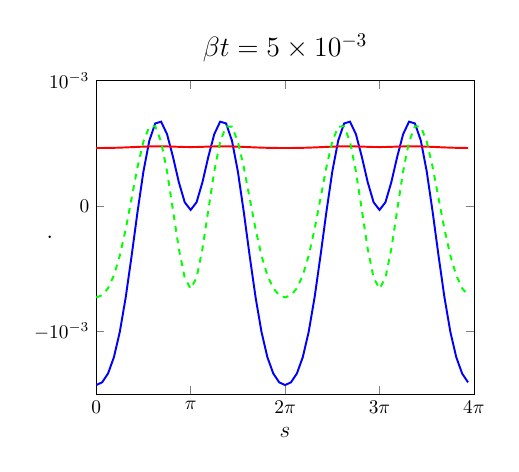
\begin{tikzpicture}[scale=0.7]

\begin{axis}[
    xmin = 0,
    xmax = 6.2832,
    xtick = {0,1.5708,3.1416,4.7124,6.2832},
    xticklabels = {$0$, $\pi$, $2\pi$, $3\pi$, $4\pi$},
    xlabel = {\large $s$},
    ymin = -0.0015,
    ymax = +0.001,
    ytick = {-0.001,0,0.001},
    yticklabels = {$-10^{-3}$,$0$,$10^{-3}$},
    ylabel = {\large $\uu \cdot \nn$},
    ylabel near ticks,
    ylabel shift = {-18pt},
    scaled y ticks = false,
    title = {\Large $\beta t = 5 \times 10^{-3}$},
  ]

\addplot[blue, line width=1pt] coordinates{
(0.0000e+00,-1.4252e-03)
(9.8175e-02,-1.4035e-03)
(1.9635e-01,-1.3334e-03)
(2.9452e-01,-1.2031e-03)
(3.9270e-01,-1.0011e-03)
(4.9087e-01,-7.2625e-04)
(5.8905e-01,-3.9562e-04)
(6.8722e-01,-4.5522e-05)
(7.8540e-01,2.7595e-04)
(8.8357e-01,5.2203e-04)
(9.8175e-01,6.5904e-04)
(1.0799e+00,6.7307e-04)
(1.1781e+00,5.7336e-04)
(1.2763e+00,3.9382e-04)
(1.3744e+00,1.9062e-04)
(1.4726e+00,3.0662e-05)
(1.5708e+00,-3.0007e-05)
(1.6690e+00,3.0662e-05)
(1.7671e+00,1.9062e-04)
(1.8653e+00,3.9382e-04)
(1.9635e+00,5.7336e-04)
(2.0617e+00,6.7307e-04)
(2.1598e+00,6.5904e-04)
(2.2580e+00,5.2203e-04)
(2.3562e+00,2.7595e-04)
(2.4544e+00,-4.5522e-05)
(2.5525e+00,-3.9562e-04)
(2.6507e+00,-7.2625e-04)
(2.7489e+00,-1.0011e-03)
(2.8471e+00,-1.2031e-03)
(2.9452e+00,-1.3334e-03)
(3.0434e+00,-1.4035e-03)
(3.1416e+00,-1.4252e-03)
(3.2398e+00,-1.4035e-03)
(3.3379e+00,-1.3334e-03)
(3.4361e+00,-1.2031e-03)
(3.5343e+00,-1.0011e-03)
(3.6325e+00,-7.2625e-04)
(3.7306e+00,-3.9562e-04)
(3.8288e+00,-4.5522e-05)
(3.9270e+00,2.7595e-04)
(4.0252e+00,5.2203e-04)
(4.1233e+00,6.5904e-04)
(4.2215e+00,6.7307e-04)
(4.3197e+00,5.7336e-04)
(4.4179e+00,3.9382e-04)
(4.5160e+00,1.9062e-04)
(4.6142e+00,3.0662e-05)
(4.7124e+00,-3.0007e-05)
(4.8106e+00,3.0662e-05)
(4.9087e+00,1.9062e-04)
(5.0069e+00,3.9382e-04)
(5.1051e+00,5.7336e-04)
(5.2033e+00,6.7307e-04)
(5.3014e+00,6.5904e-04)
(5.3996e+00,5.2203e-04)
(5.4978e+00,2.7595e-04)
(5.5960e+00,-4.5522e-05)
(5.6941e+00,-3.9562e-04)
(5.7923e+00,-7.2625e-04)
(5.8905e+00,-1.0011e-03)
(5.9887e+00,-1.2031e-03)
(6.0868e+00,-1.3334e-03)
(6.1850e+00,-1.4035e-03)
};

\addplot[red, line width=1pt] coordinates{
(0.0000e+00,4.6324e-04)
(9.8175e-02,4.6339e-04)
(1.9635e-01,4.6387e-04)
(2.9452e-01,4.6475e-04)
(3.9270e-01,4.6609e-04)
(4.9087e-01,4.6787e-04)
(5.8905e-01,4.6994e-04)
(6.8722e-01,4.7207e-04)
(7.8540e-01,4.7399e-04)
(8.8357e-01,4.7546e-04)
(9.8175e-01,4.7630e-04)
(1.0799e+00,4.7637e-04)
(1.1781e+00,4.7565e-04)
(1.2763e+00,4.7429e-04)
(1.3744e+00,4.7265e-04)
(1.4726e+00,4.7130e-04)
(1.5708e+00,4.7077e-04)
(1.6690e+00,4.7130e-04)
(1.7671e+00,4.7265e-04)
(1.8653e+00,4.7429e-04)
(1.9635e+00,4.7565e-04)
(2.0617e+00,4.7637e-04)
(2.1598e+00,4.7630e-04)
(2.2580e+00,4.7546e-04)
(2.3562e+00,4.7399e-04)
(2.4544e+00,4.7207e-04)
(2.5525e+00,4.6994e-04)
(2.6507e+00,4.6787e-04)
(2.7489e+00,4.6609e-04)
(2.8471e+00,4.6475e-04)
(2.9452e+00,4.6387e-04)
(3.0434e+00,4.6339e-04)
(3.1416e+00,4.6324e-04)
(3.2398e+00,4.6339e-04)
(3.3379e+00,4.6387e-04)
(3.4361e+00,4.6475e-04)
(3.5343e+00,4.6609e-04)
(3.6325e+00,4.6787e-04)
(3.7306e+00,4.6994e-04)
(3.8288e+00,4.7207e-04)
(3.9270e+00,4.7399e-04)
(4.0252e+00,4.7546e-04)
(4.1233e+00,4.7630e-04)
(4.2215e+00,4.7637e-04)
(4.3197e+00,4.7565e-04)
(4.4179e+00,4.7429e-04)
(4.5160e+00,4.7265e-04)
(4.6142e+00,4.7130e-04)
(4.7124e+00,4.7077e-04)
(4.8106e+00,4.7130e-04)
(4.9087e+00,4.7265e-04)
(5.0069e+00,4.7429e-04)
(5.1051e+00,4.7565e-04)
(5.2033e+00,4.7637e-04)
(5.3014e+00,4.7630e-04)
(5.3996e+00,4.7546e-04)
(5.4978e+00,4.7399e-04)
(5.5960e+00,4.7207e-04)
(5.6941e+00,4.6994e-04)
(5.7923e+00,4.6787e-04)
(5.8905e+00,4.6609e-04)
(5.9887e+00,4.6475e-04)
(6.0868e+00,4.6387e-04)
(6.1850e+00,4.6339e-04)
};

\addplot[green, dashed, line width=1pt] coordinates{
(0.0000e+00,-7.2674e-04)
(9.8175e-02,-7.0951e-04)
(1.9635e-01,-6.5403e-04)
(2.9452e-01,-5.5135e-04)
(3.9270e-01,-3.9376e-04)
(4.9087e-01,-1.8298e-04)
(5.8905e-01,6.3302e-05)
(6.8722e-01,3.1063e-04)
(7.8540e-01,5.1478e-04)
(8.8357e-01,6.3332e-04)
(9.8175e-01,6.3615e-04)
(1.0799e+00,5.1265e-04)
(1.1781e+00,2.7661e-04)
(1.2763e+00,-3.0169e-05)
(1.3744e+00,-3.3971e-04)
(1.4726e+00,-5.7126e-04)
(1.5708e+00,-6.5729e-04)
(1.6690e+00,-5.7126e-04)
(1.7671e+00,-3.3971e-04)
(1.8653e+00,-3.0169e-05)
(1.9635e+00,2.7661e-04)
(2.0617e+00,5.1265e-04)
(2.1598e+00,6.3615e-04)
(2.2580e+00,6.3332e-04)
(2.3562e+00,5.1478e-04)
(2.4544e+00,3.1063e-04)
(2.5525e+00,6.3302e-05)
(2.6507e+00,-1.8298e-04)
(2.7489e+00,-3.9376e-04)
(2.8471e+00,-5.5135e-04)
(2.9452e+00,-6.5403e-04)
(3.0434e+00,-7.0951e-04)
(3.1416e+00,-7.2674e-04)
(3.2398e+00,-7.0951e-04)
(3.3379e+00,-6.5403e-04)
(3.4361e+00,-5.5135e-04)
(3.5343e+00,-3.9376e-04)
(3.6325e+00,-1.8298e-04)
(3.7306e+00,6.3302e-05)
(3.8288e+00,3.1063e-04)
(3.9270e+00,5.1478e-04)
(4.0252e+00,6.3332e-04)
(4.1233e+00,6.3615e-04)
(4.2215e+00,5.1265e-04)
(4.3197e+00,2.7661e-04)
(4.4179e+00,-3.0169e-05)
(4.5160e+00,-3.3971e-04)
(4.6142e+00,-5.7126e-04)
(4.7124e+00,-6.5729e-04)
(4.8106e+00,-5.7126e-04)
(4.9087e+00,-3.3971e-04)
(5.0069e+00,-3.0169e-05)
(5.1051e+00,2.7661e-04)
(5.2033e+00,5.1265e-04)
(5.3014e+00,6.3615e-04)
(5.3996e+00,6.3332e-04)
(5.4978e+00,5.1478e-04)
(5.5960e+00,3.1063e-04)
(5.6941e+00,6.3302e-05)
(5.7923e+00,-1.8298e-04)
(5.8905e+00,-3.9376e-04)
(5.9887e+00,-5.5135e-04)
(6.0868e+00,-6.5403e-04)
(6.1850e+00,-7.0951e-04)
};

\end{axis}


\end{tikzpicture}

%  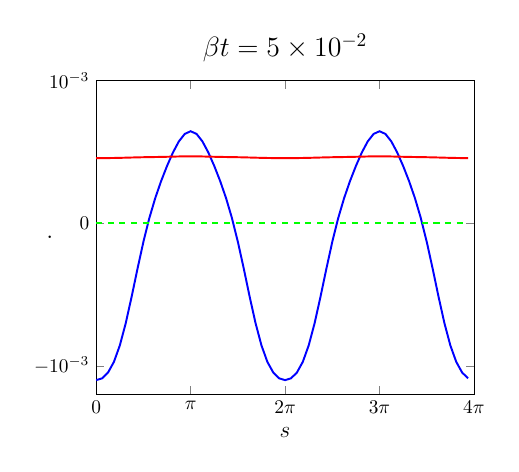
\begin{tikzpicture}[scale=0.7]


\begin{axis}[
    xmin = 0,
    xmax = 6.2832,
    xtick = {0,1.5708,3.1416,4.7124,6.2832},
    xticklabels = {$0$, $\pi$, $2\pi$, $3\pi$, $4\pi$},
    xlabel = {\large $s$},
    ymin = -0.0012,
    ymax = +0.001,
    ytick = {-0.001,0,0.001},
    yticklabels = {$-10^{-3}$,$0$,$10^{-3}$},
    ylabel = {\large $\uu \cdot \nn$},
    ylabel near ticks,
    ylabel shift = {-18pt},
    scaled y ticks = false,
    title = {\Large $\beta t = 5 \times 10^{-2}$},
  ]

\addplot[blue, line width=1pt] coordinates{
(0.0000e+00,-1.0996e-03)
(9.8175e-02,-1.0870e-03)
(1.9635e-01,-1.0466e-03)
(2.9452e-01,-9.7170e-04)
(3.9270e-01,-8.5638e-04)
(4.9087e-01,-7.0082e-04)
(5.8905e-01,-5.1507e-04)
(6.8722e-01,-3.1782e-04)
(7.8540e-01,-1.2954e-04)
(8.8357e-01,3.6091e-05)
(9.8175e-01,1.7622e-04)
(1.0799e+00,2.9597e-04)
(1.1781e+00,4.0183e-04)
(1.2763e+00,4.9586e-04)
(1.3744e+00,5.7370e-04)
(1.4726e+00,6.2639e-04)
(1.5708e+00,6.4517e-04)
(1.6690e+00,6.2639e-04)
(1.7671e+00,5.7370e-04)
(1.8653e+00,4.9586e-04)
(1.9635e+00,4.0183e-04)
(2.0617e+00,2.9597e-04)
(2.1598e+00,1.7622e-04)
(2.2580e+00,3.6091e-05)
(2.3562e+00,-1.2954e-04)
(2.4544e+00,-3.1782e-04)
(2.5525e+00,-5.1507e-04)
(2.6507e+00,-7.0082e-04)
(2.7489e+00,-8.5638e-04)
(2.8471e+00,-9.7170e-04)
(2.9452e+00,-1.0466e-03)
(3.0434e+00,-1.0870e-03)
(3.1416e+00,-1.0996e-03)
(3.2398e+00,-1.0870e-03)
(3.3379e+00,-1.0466e-03)
(3.4361e+00,-9.7170e-04)
(3.5343e+00,-8.5638e-04)
(3.6325e+00,-7.0082e-04)
(3.7306e+00,-5.1507e-04)
(3.8288e+00,-3.1782e-04)
(3.9270e+00,-1.2954e-04)
(4.0252e+00,3.6091e-05)
(4.1233e+00,1.7622e-04)
(4.2215e+00,2.9597e-04)
(4.3197e+00,4.0183e-04)
(4.4179e+00,4.9586e-04)
(4.5160e+00,5.7370e-04)
(4.6142e+00,6.2639e-04)
(4.7124e+00,6.4517e-04)
(4.8106e+00,6.2639e-04)
(4.9087e+00,5.7370e-04)
(5.0069e+00,4.9586e-04)
(5.1051e+00,4.0183e-04)
(5.2033e+00,2.9597e-04)
(5.3014e+00,1.7622e-04)
(5.3996e+00,3.6091e-05)
(5.4978e+00,-1.2954e-04)
(5.5960e+00,-3.1782e-04)
(5.6941e+00,-5.1507e-04)
(5.7923e+00,-7.0082e-04)
(5.8905e+00,-8.5638e-04)
(5.9887e+00,-9.7170e-04)
(6.0868e+00,-1.0466e-03)
(6.1850e+00,-1.0870e-03)
};

\addplot[red, line width=1pt] coordinates{
(0.0000e+00,4.5667e-04)
(9.8175e-02,4.5678e-04)
(1.9635e-01,4.5711e-04)
(2.9452e-01,4.5772e-04)
(3.9270e-01,4.5862e-04)
(4.9087e-01,4.5975e-04)
(5.8905e-01,4.6097e-04)
(6.8722e-01,4.6210e-04)
(7.8540e-01,4.6302e-04)
(8.8357e-01,4.6376e-04)
(9.8175e-01,4.6444e-04)
(1.0799e+00,4.6521e-04)
(1.1781e+00,4.6616e-04)
(1.2763e+00,4.6723e-04)
(1.3744e+00,4.6829e-04)
(1.4726e+00,4.6908e-04)
(1.5708e+00,4.6938e-04)
(1.6690e+00,4.6908e-04)
(1.7671e+00,4.6829e-04)
(1.8653e+00,4.6723e-04)
(1.9635e+00,4.6616e-04)
(2.0617e+00,4.6521e-04)
(2.1598e+00,4.6444e-04)
(2.2580e+00,4.6376e-04)
(2.3562e+00,4.6302e-04)
(2.4544e+00,4.6210e-04)
(2.5525e+00,4.6097e-04)
(2.6507e+00,4.5975e-04)
(2.7489e+00,4.5862e-04)
(2.8471e+00,4.5772e-04)
(2.9452e+00,4.5711e-04)
(3.0434e+00,4.5678e-04)
(3.1416e+00,4.5667e-04)
(3.2398e+00,4.5678e-04)
(3.3379e+00,4.5711e-04)
(3.4361e+00,4.5772e-04)
(3.5343e+00,4.5862e-04)
(3.6325e+00,4.5975e-04)
(3.7306e+00,4.6097e-04)
(3.8288e+00,4.6210e-04)
(3.9270e+00,4.6302e-04)
(4.0252e+00,4.6376e-04)
(4.1233e+00,4.6444e-04)
(4.2215e+00,4.6521e-04)
(4.3197e+00,4.6616e-04)
(4.4179e+00,4.6723e-04)
(4.5160e+00,4.6829e-04)
(4.6142e+00,4.6908e-04)
(4.7124e+00,4.6938e-04)
(4.8106e+00,4.6908e-04)
(4.9087e+00,4.6829e-04)
(5.0069e+00,4.6723e-04)
(5.1051e+00,4.6616e-04)
(5.2033e+00,4.6521e-04)
(5.3014e+00,4.6444e-04)
(5.3996e+00,4.6376e-04)
(5.4978e+00,4.6302e-04)
(5.5960e+00,4.6210e-04)
(5.6941e+00,4.6097e-04)
(5.7923e+00,4.5975e-04)
(5.8905e+00,4.5862e-04)
(5.9887e+00,4.5772e-04)
(6.0868e+00,4.5711e-04)
(6.1850e+00,4.5678e-04)
};

\addplot[green, dashed, line width=1pt] coordinates{
(0.0000e+00,-2.3701e-12)
(9.8175e-02,-5.1013e-12)
(1.9635e-01,-2.1890e-12)
(2.9452e-01,-3.5219e-12)
(3.9270e-01,-1.5410e-12)
(4.9087e-01,-1.8243e-12)
(5.8905e-01,-4.6256e-13)
(6.8722e-01,8.3140e-13)
(7.8540e-01,1.0570e-12)
(8.8357e-01,2.3248e-12)
(9.8175e-01,2.1470e-12)
(1.0799e+00,3.2332e-12)
(1.1781e+00,2.3841e-12)
(1.2763e+00,3.6752e-12)
(1.3744e+00,2.7500e-12)
(1.4726e+00,3.8911e-12)
(1.5708e+00,3.0465e-12)
(1.6690e+00,3.7839e-12)
(1.7671e+00,2.9670e-12)
(1.8653e+00,3.3832e-12)
(1.9635e+00,2.5833e-12)
(2.0617e+00,3.1272e-12)
(2.1598e+00,1.9943e-12)
(2.2580e+00,2.8072e-12)
(2.3562e+00,4.5835e-13)
(2.4544e+00,1.8049e-12)
(2.5525e+00,-1.7784e-12)
(2.6507e+00,4.5430e-13)
(2.7489e+00,-4.4271e-12)
(2.8471e+00,-1.2356e-12)
(2.9452e+00,-4.6053e-12)
(3.0434e+00,-2.1283e-12)
(3.1416e+00,-5.5059e-12)
(3.2398e+00,-3.2576e-12)
(3.3379e+00,-2.5917e-12)
(3.4361e+00,-3.6846e-12)
(3.5343e+00,-1.2203e-12)
(3.6325e+00,-2.5257e-12)
(3.7306e+00,4.3051e-13)
(3.8288e+00,-1.0295e-13)
(3.9270e+00,2.0464e-12)
(4.0252e+00,1.3831e-12)
(4.1233e+00,3.1439e-12)
(4.2215e+00,2.1068e-12)
(4.3197e+00,3.5191e-12)
(4.4179e+00,2.5897e-12)
(4.5160e+00,3.8035e-12)
(4.6142e+00,2.9385e-12)
(4.7124e+00,3.9496e-12)
(4.8106e+00,2.9646e-12)
(4.9087e+00,3.7350e-12)
(5.0069e+00,2.6137e-12)
(5.1051e+00,3.3981e-12)
(5.2033e+00,2.3594e-12)
(5.3014e+00,2.9610e-12)
(5.3996e+00,1.6281e-12)
(5.4978e+00,1.7719e-12)
(5.5960e+00,1.6160e-13)
(5.6941e+00,-2.2854e-13)
(5.7923e+00,-1.1349e-12)
(5.8905e+00,-2.8796e-12)
(5.9887e+00,-2.9905e-12)
(6.0868e+00,-2.1672e-12)
(6.1850e+00,-5.0508e-12)
};

\end{axis}

\end{tikzpicture}

%%  \fi
%  \caption{\label{fig:vesVelocity} The velocity contributions due to
%  semi-permeability (red) and force balance (blue). The green dashed
%  line is the velocity of an impermeable vesicle with the same initial
%  shape as the semi-permeable vesicle.}
%\end{figure}
%
%\begin{figure}[htp]
%%  \ifTikz
%  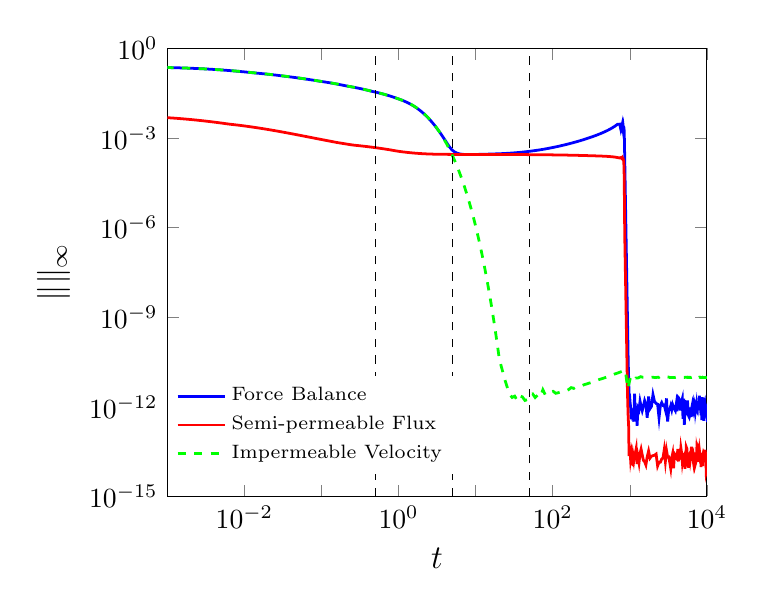
\begin{tikzpicture}[scale=1]

  \begin{axis}[
    name = maxPlot,
    xmin = 1e-3,
    xmax = 10000,
    ymin = 1e-15,
    ymax = 1e0,
    xmode = log,
    ymode = log,
    xminorticks = false,
    yminorticks = false,
    xtick = {1e-3,1e-2,1e-1,1e0,1e1,1e2,1e3,1e4},
    xticklabels = {,$10^{-2}$,,$10^0$,,$10^2$,,$10^4$},
    xlabel = {\large $t$},
    ylabel = {\large $\|\uu\|_\infty$},
    ylabel near ticks,
    legend entries = {Force Balance,
    Semi-permeable Flux,Impermeable Velocity},
    legend cell align=left,
    legend style={draw=none,font=\scriptsize},
    legend style={at={(0.0,0.05)},anchor=south west}
  ]

\addplot[blue, line width=1pt] coordinates{
(0.0000e+00,2.5143e-01)
(6.4149e-05,2.4906e-01)
(1.2188e-04,2.4693e-01)
(1.8424e-04,2.4478e-01)
(2.5158e-04,2.4254e-01)
(3.2431e-04,2.4022e-01)
(4.0286e-04,2.3783e-01)
(4.8769e-04,2.3537e-01)
(5.7930e-04,2.3284e-01)
(6.7825e-04,2.3024e-01)
(7.8511e-04,2.2773e-01)
(9.0052e-04,2.2619e-01)
(1.0252e-03,2.2455e-01)
(1.1598e-03,2.2283e-01)
(1.3052e-03,2.2100e-01)
(1.4622e-03,2.1908e-01)
(1.6318e-03,2.1706e-01)
(1.8149e-03,2.1494e-01)
(2.0127e-03,2.1273e-01)
(2.2263e-03,2.1043e-01)
(2.4570e-03,2.0804e-01)
(2.7062e-03,2.0557e-01)
(2.9753e-03,2.0301e-01)
(3.2659e-03,2.0037e-01)
(3.5798e-03,1.9766e-01)
(3.9188e-03,1.9487e-01)
(4.2849e-03,1.9201e-01)
(4.6803e-03,1.8909e-01)
(5.1073e-03,1.8610e-01)
(5.5685e-03,1.8306e-01)
(6.0666e-03,1.7997e-01)
(6.6045e-03,1.7683e-01)
(7.1855e-03,1.7365e-01)
(7.8129e-03,1.7043e-01)
(8.4905e-03,1.6718e-01)
(9.2224e-03,1.6390e-01)
(9.9991e-03,1.6066e-01)
(1.0827e-02,1.5743e-01)
(1.1702e-02,1.5426e-01)
(1.2641e-02,1.5108e-01)
(1.3621e-02,1.4800e-01)
(1.4679e-02,1.4543e-01)
(1.5779e-02,1.4296e-01)
(1.6968e-02,1.4043e-01)
(1.8208e-02,1.3794e-01)
(1.9547e-02,1.3539e-01)
(2.0933e-02,1.3290e-01)
(2.2430e-02,1.3035e-01)
(2.3996e-02,1.2782e-01)
(2.5687e-02,1.2523e-01)
(2.7422e-02,1.2273e-01)
(2.9295e-02,1.2015e-01)
(3.1276e-02,1.1758e-01)
(3.3376e-02,1.1510e-01)
(3.5593e-02,1.1281e-01)
(3.7949e-02,1.1053e-01)
(4.0425e-02,1.0827e-01)
(4.3074e-02,1.0599e-01)
(4.5826e-02,1.0377e-01)
(4.8797e-02,1.0149e-01)
(5.1865e-02,9.9283e-02)
(5.5178e-02,9.7024e-02)
(5.8630e-02,9.4806e-02)
(6.2358e-02,9.2538e-02)
(6.6187e-02,9.0543e-02)
(7.0322e-02,8.8527e-02)
(7.4666e-02,8.6516e-02)
(7.9318e-02,8.4459e-02)
(8.4141e-02,8.2434e-02)
(8.9350e-02,8.0349e-02)
(9.4748e-02,7.8401e-02)
(1.0058e-01,7.6656e-02)
(1.0663e-01,7.4942e-02)
(1.1316e-01,7.3178e-02)
(1.1994e-01,7.1447e-02)
(1.2725e-01,6.9669e-02)
(1.3486e-01,6.7918e-02)
(1.4308e-01,6.6121e-02)
(1.5159e-01,6.4360e-02)
(1.6079e-01,6.2557e-02)
(1.7039e-01,6.0778e-02)
(1.8076e-01,5.8961e-02)
(1.9148e-01,5.7215e-02)
(2.0304e-01,5.5535e-02)
(2.1521e-01,5.3906e-02)
(2.2829e-01,5.2503e-02)
(2.4187e-01,5.1119e-02)
(2.5654e-01,4.9696e-02)
(2.7191e-01,4.8285e-02)
(2.8850e-01,4.6839e-02)
(3.0579e-01,4.5415e-02)
(3.2446e-01,4.3960e-02)
(3.4425e-01,4.2507e-02)
(3.6555e-01,4.1032e-02)
(3.8802e-01,3.9571e-02)
(4.1229e-01,3.8090e-02)
(4.3823e-01,3.6663e-02)
(4.6618e-01,3.5256e-02)
(4.9600e-01,3.4003e-02)
(5.2821e-01,3.2752e-02)
(5.6259e-01,3.1488e-02)
(5.9972e-01,3.0196e-02)
(6.3901e-01,2.8902e-02)
(6.8145e-01,2.7582e-02)
(7.2600e-01,2.6334e-02)
(7.7412e-01,2.5064e-02)
(8.2397e-01,2.3816e-02)
(8.7782e-01,2.2537e-02)
(9.3363e-01,2.1296e-02)
(9.9391e-01,2.0088e-02)
(1.0560e+00,1.8988e-02)
(1.1231e+00,1.7874e-02)
(1.1935e+00,1.6761e-02)
(1.2696e+00,1.5602e-02)
(1.3493e+00,1.4457e-02)
(1.4353e+00,1.3282e-02)
(1.5282e+00,1.2101e-02)
(1.6286e+00,1.0921e-02)
(1.7370e+00,9.7569e-03)
(1.8540e+00,8.6206e-03)
(1.9805e+00,7.5269e-03)
(2.1170e+00,6.4886e-03)
(2.2645e+00,5.5180e-03)
(2.4237e+00,4.6252e-03)
(2.5957e+00,3.8178e-03)
(2.7815e+00,3.1018e-03)
(2.9821e+00,2.4840e-03)
(3.1988e+00,1.9590e-03)
(3.4328e+00,1.5197e-03)
(3.6855e+00,1.1615e-03)
(3.9584e+00,8.7926e-04)
(4.2532e+00,6.5945e-04)
(4.5716e+00,4.9988e-04)
(4.9154e+00,3.9480e-04)
(5.2868e+00,3.4142e-04)
(5.6878e+00,3.0992e-04)
(6.1209e+00,2.9209e-04)
(6.5887e+00,2.8332e-04)
(7.0939e+00,2.7818e-04)
(7.6395e+00,2.7687e-04)
(8.2288e+00,2.7653e-04)
(8.8652e+00,2.7680e-04)
(9.5525e+00,2.7748e-04)
(1.0295e+01,2.7843e-04)
(1.1096e+01,2.7956e-04)
(1.1962e+01,2.8085e-04)
(1.2897e+01,2.8227e-04)
(1.3907e+01,2.8381e-04)
(1.4998e+01,2.8549e-04)
(1.6176e+01,2.8731e-04)
(1.7448e+01,2.8927e-04)
(1.8822e+01,2.9140e-04)
(2.0306e+01,2.9371e-04)
(2.1908e+01,2.9620e-04)
(2.3639e+01,2.9906e-04)
(2.5509e+01,3.0232e-04)
(2.7527e+01,3.0615e-04)
(2.9708e+01,3.1030e-04)
(3.2062e+01,3.1485e-04)
(3.4605e+01,3.2004e-04)
(3.7352e+01,3.2577e-04)
(4.0318e+01,3.3238e-04)
(4.3522e+01,3.3966e-04)
(4.6982e+01,3.4754e-04)
(5.0718e+01,3.5606e-04)
(5.4754e+01,3.6529e-04)
(5.9112e+01,3.7527e-04)
(6.3819e+01,3.8609e-04)
(6.8903e+01,3.9780e-04)
(7.4393e+01,4.1106e-04)
(8.0323e+01,4.2566e-04)
(8.6727e+01,4.4148e-04)
(9.3643e+01,4.5860e-04)
(1.0111e+02,4.7716e-04)
(1.0918e+02,4.9728e-04)
(1.1789e+02,5.1910e-04)
(1.2730e+02,5.4279e-04)
(1.3746e+02,5.6851e-04)
(1.4844e+02,5.9648e-04)
(1.6029e+02,6.2690e-04)
(1.7309e+02,6.6004e-04)
(1.8692e+02,6.9619e-04)
(2.0185e+02,7.3567e-04)
(2.1798e+02,7.7888e-04)
(2.3539e+02,8.2627e-04)
(2.5420e+02,8.7860e-04)
(2.7452e+02,9.3646e-04)
(2.9646e+02,1.0004e-03)
(3.2015e+02,1.0713e-03)
(3.4574e+02,1.1504e-03)
(3.7338e+02,1.2392e-03)
(4.0323e+02,1.3396e-03)
(4.3546e+02,1.4544e-03)
(4.7028e+02,1.5874e-03)
(5.0788e+02,1.7443e-03)
(5.4849e+02,1.9321e-03)
(5.9234e+02,2.1625e-03)
(6.3971e+02,2.4532e-03)
(6.9087e+02,2.8309e-03)
(7.3860e+02,2.8717e-03)
(7.6471e+02,1.8870e-03)
(7.8821e+02,2.5831e-03)
(7.9978e+02,1.5132e-03)
(8.1019e+02,2.1951e-03)
(8.1786e+02,1.8397e-03)
(8.2476e+02,2.1848e-03)
(8.2894e+02,1.9639e-03)
(8.3270e+02,2.1935e-03)
(8.3676e+02,2.1955e-03)
(8.4008e+02,2.0963e-03)
(8.4307e+02,1.8359e-03)
(8.4630e+02,1.3692e-03)
(8.4979e+02,8.5321e-04)
(8.5355e+02,4.6151e-04)
(8.5762e+02,2.2880e-04)
(8.6201e+02,1.0623e-04)
(8.6676e+02,4.6574e-05)
(8.7188e+02,1.9205e-05)
(8.7741e+02,7.4416e-06)
(8.8339e+02,2.6891e-06)
(8.8984e+02,9.0581e-07)
(8.9681e+02,2.8105e-07)
(9.0434e+02,8.0677e-08)
(9.1247e+02,2.0930e-08)
(9.2125e+02,5.0195e-09)
(9.3074e+02,1.0411e-09)
(9.4098e+02,2.1553e-10)
(9.5204e+02,3.3127e-11)
(9.6399e+02,1.0173e-11)
(9.7689e+02,2.6156e-12)
(9.9082e+02,2.5647e-12)
(1.0059e+03,1.4604e-12)
(1.0221e+03,1.0297e-12)
(1.0397e+03,3.8532e-13)
(1.0586e+03,8.7966e-13)
(1.0791e+03,5.6448e-13)
(1.1012e+03,6.7332e-13)
(1.1251e+03,3.1864e-13)
(1.1509e+03,2.7655e-12)
(1.1787e+03,4.3047e-13)
(1.2088e+03,9.2874e-13)
(1.2413e+03,2.3389e-13)
(1.2764e+03,9.1925e-13)
(1.3143e+03,7.9248e-13)
(1.3552e+03,1.5394e-12)
(1.3994e+03,1.0368e-12)
(1.4472e+03,7.4452e-13)
(1.4987e+03,1.0463e-12)
(1.5544e+03,1.6068e-12)
(1.6145e+03,1.2030e-12)
(1.6795e+03,4.3113e-13)
(1.7496e+03,2.2264e-12)
(1.8254e+03,8.6291e-13)
(1.9072e+03,1.0332e-12)
(1.9955e+03,2.5592e-12)
(2.0910e+03,1.4926e-12)
(2.1910e+03,1.3019e-12)
(2.2910e+03,1.2244e-12)
(2.3910e+03,4.2932e-13)
(2.4910e+03,1.1290e-12)
(2.5910e+03,1.3855e-12)
(2.6910e+03,1.1209e-12)
(2.7910e+03,1.1519e-12)
(2.8910e+03,7.9919e-13)
(2.9910e+03,1.9182e-12)
(3.0910e+03,3.2355e-13)
(3.1910e+03,7.8306e-13)
(3.2910e+03,8.0543e-13)
(3.3910e+03,1.0720e-12)
(3.4910e+03,7.9869e-13)
(3.5910e+03,1.1848e-12)
(3.6910e+03,9.7610e-13)
(3.7910e+03,8.4733e-13)
(3.8910e+03,7.4753e-13)
(3.9910e+03,1.1734e-12)
(4.0910e+03,7.0933e-13)
(4.1910e+03,2.1420e-12)
(4.2910e+03,2.0005e-12)
(4.3910e+03,1.7126e-12)
(4.4910e+03,8.2398e-13)
(4.5910e+03,8.2245e-13)
(4.6910e+03,1.5379e-12)
(4.7910e+03,1.8778e-12)
(4.8910e+03,3.9299e-13)
(4.9910e+03,1.8851e-12)
(5.0910e+03,2.5074e-13)
(5.1910e+03,9.8207e-13)
(5.2910e+03,9.0016e-13)
(5.3910e+03,1.6474e-12)
(5.4910e+03,5.2017e-13)
(5.5910e+03,1.6420e-12)
(5.6910e+03,7.9097e-13)
(5.7910e+03,4.9046e-13)
(5.8910e+03,4.4748e-13)
(5.9910e+03,5.4278e-13)
(6.0910e+03,9.5033e-13)
(6.1910e+03,4.5112e-13)
(6.2910e+03,8.8500e-13)
(6.3910e+03,1.0037e-12)
(6.4910e+03,1.2334e-12)
(6.5910e+03,9.5577e-13)
(6.6910e+03,1.4078e-12)
(6.7910e+03,4.8365e-13)
(6.8910e+03,1.3804e-12)
(6.9910e+03,1.2211e-12)
(7.0910e+03,7.2179e-13)
(7.1910e+03,9.3724e-13)
(7.2910e+03,1.1978e-12)
(7.3910e+03,7.6460e-13)
(7.4910e+03,7.1138e-13)
(7.5910e+03,1.4478e-12)
(7.6910e+03,9.7540e-13)
(7.7910e+03,9.4444e-13)
(7.8910e+03,7.7455e-13)
(7.9910e+03,2.3758e-12)
(8.0910e+03,1.3559e-12)
(8.1910e+03,8.2851e-13)
(8.2910e+03,7.7395e-13)
(8.3910e+03,5.2508e-13)
(8.4910e+03,1.5877e-12)
(8.5910e+03,3.6241e-13)
(8.6910e+03,2.0898e-12)
(8.7910e+03,1.1283e-12)
(8.8910e+03,5.7107e-13)
(8.9910e+03,8.8000e-13)
(9.0910e+03,3.4033e-13)
(9.1910e+03,1.9988e-12)
(9.2910e+03,1.2492e-12)
(9.3910e+03,1.3974e-12)
(9.4910e+03,1.1016e-12)
(9.5910e+03,8.3162e-13)
(9.6910e+03,9.6957e-13)
(9.7910e+03,9.9004e-13)
(9.8910e+03,1.1992e-12)
(9.9910e+03,7.0748e-13)
(1.0091e+04,8.0575e-13)
(1.0191e+04,4.0864e-13)
(1.0291e+04,3.1129e-13)
(1.0391e+04,5.2996e-13)
(1.0491e+04,2.2481e-12)
(1.0591e+04,7.9016e-13)
(1.0691e+04,9.1354e-13)
(1.0791e+04,4.7389e-13)
(1.0891e+04,6.1893e-13)
(1.0991e+04,1.8346e-12)
(1.1091e+04,1.5432e-12)
(1.1191e+04,9.1388e-13)
(1.1291e+04,8.0937e-13)
(1.1391e+04,1.5291e-12)
(1.1491e+04,8.5536e-13)
(1.1591e+04,1.9577e-12)
(1.1691e+04,8.2352e-13)
(1.1791e+04,1.0942e-12)
(1.1891e+04,9.8388e-13)
(1.1991e+04,1.6554e-12)
(1.2091e+04,1.3927e-12)
(1.2191e+04,9.2175e-13)
(1.2291e+04,1.0800e-12)
(1.2391e+04,6.8912e-13)
(1.2491e+04,6.7045e-13)
(1.2591e+04,1.3170e-12)
(1.2691e+04,1.0000e-12)
(1.2791e+04,6.0368e-13)
(1.2891e+04,4.6551e-13)
(1.2991e+04,4.2708e-13)
(1.3091e+04,7.9265e-13)
(1.3191e+04,1.0978e-12)
(1.3291e+04,1.0257e-12)
(1.3391e+04,5.0769e-13)
(1.3491e+04,1.4083e-12)
(1.3591e+04,8.9094e-13)
(1.3691e+04,1.4698e-12)
(1.3791e+04,9.7415e-13)
(1.3891e+04,8.7689e-13)
(1.3991e+04,6.3129e-13)
(1.4091e+04,7.5509e-13)
(1.4191e+04,1.8049e-12)
(1.4291e+04,5.0680e-13)
(1.4391e+04,1.2294e-12)
(1.4491e+04,1.5597e-12)
(1.4591e+04,5.4681e-13)
(1.4691e+04,9.8953e-13)
(1.4791e+04,1.1934e-12)
(1.4891e+04,1.7594e-12)
(1.4991e+04,1.6216e-12)
(1.5091e+04,7.2236e-13)
(1.5191e+04,1.9573e-12)
(1.5291e+04,4.4939e-13)
(1.5391e+04,1.4691e-12)
(1.5491e+04,1.2943e-12)
(1.5591e+04,2.4329e-12)
(1.5691e+04,1.6416e-12)
(1.5791e+04,1.2694e-12)
(1.5891e+04,8.1613e-13)
(1.5991e+04,6.8194e-13)
(1.6091e+04,1.5994e-12)
(1.6191e+04,3.7993e-13)
(1.6291e+04,1.3779e-12)
(1.6391e+04,1.2776e-12)
(1.6491e+04,5.6385e-13)
(1.6591e+04,1.6089e-12)
(1.6691e+04,2.0244e-12)
(1.6791e+04,2.0989e-12)
(1.6891e+04,1.7240e-12)
(1.6991e+04,1.4830e-12)
(1.7091e+04,1.5747e-12)
(1.7191e+04,1.5543e-12)
(1.7291e+04,7.0006e-13)
(1.7391e+04,1.3472e-12)
(1.7491e+04,3.4862e-13)
(1.7591e+04,1.2367e-12)
(1.7691e+04,7.0192e-13)
(1.7791e+04,6.6082e-13)
(1.7891e+04,4.8511e-13)
(1.7991e+04,1.3491e-12)
(1.8091e+04,6.3469e-13)
(1.8191e+04,1.9423e-12)
(1.8291e+04,1.2199e-12)
(1.8391e+04,8.7569e-13)
(1.8491e+04,8.7707e-13)
(1.8591e+04,1.4653e-12)
(1.8691e+04,1.7261e-12)
(1.8791e+04,1.2364e-12)
(1.8891e+04,7.5528e-13)
(1.8991e+04,4.3179e-13)
(1.9091e+04,6.1800e-13)
(1.9191e+04,1.5140e-12)
(1.9291e+04,9.4249e-13)
(1.9391e+04,9.7265e-13)
(1.9491e+04,1.2219e-12)
(1.9591e+04,5.4964e-13)
(1.9691e+04,1.7148e-12)
(1.9791e+04,9.5472e-13)
(1.9891e+04,8.7837e-13)
(1.9991e+04,3.7547e-13)
(2.0000e+04,4.7031e-13)
};

\addplot[red, line width=1pt] coordinates{
(0.0000e+00,5.6693e-03)
(6.4149e-05,5.6070e-03)
(1.2188e-04,5.5480e-03)
(1.8424e-04,5.4839e-03)
(2.5158e-04,5.4139e-03)
(3.2431e-04,5.3388e-03)
(4.0286e-04,5.2588e-03)
(4.8769e-04,5.1745e-03)
(5.7930e-04,5.0862e-03)
(6.7825e-04,4.9945e-03)
(7.8511e-04,4.8999e-03)
(9.0052e-04,4.8029e-03)
(1.0252e-03,4.7041e-03)
(1.1598e-03,4.6038e-03)
(1.3052e-03,4.5025e-03)
(1.4622e-03,4.4006e-03)
(1.6318e-03,4.2983e-03)
(1.8149e-03,4.1958e-03)
(2.0127e-03,4.0934e-03)
(2.2263e-03,3.9913e-03)
(2.4570e-03,3.8896e-03)
(2.7062e-03,3.7884e-03)
(2.9753e-03,3.6879e-03)
(3.2659e-03,3.5882e-03)
(3.5798e-03,3.4893e-03)
(3.9188e-03,3.3914e-03)
(4.2849e-03,3.2947e-03)
(4.6803e-03,3.1991e-03)
(5.1073e-03,3.1048e-03)
(5.5685e-03,3.0120e-03)
(6.0666e-03,2.9206e-03)
(6.6045e-03,2.8397e-03)
(7.1855e-03,2.7728e-03)
(7.8129e-03,2.7048e-03)
(8.4905e-03,2.6360e-03)
(9.2224e-03,2.5666e-03)
(9.9991e-03,2.4980e-03)
(1.0827e-02,2.4299e-03)
(1.1702e-02,2.3632e-03)
(1.2641e-02,2.2969e-03)
(1.3621e-02,2.2328e-03)
(1.4679e-02,2.1688e-03)
(1.5779e-02,2.1072e-03)
(1.6968e-02,2.0459e-03)
(1.8208e-02,1.9868e-03)
(1.9547e-02,1.9280e-03)
(2.0933e-02,1.8720e-03)
(2.2430e-02,1.8163e-03)
(2.3996e-02,1.7626e-03)
(2.5687e-02,1.7094e-03)
(2.7422e-02,1.6591e-03)
(2.9295e-02,1.6092e-03)
(3.1276e-02,1.5608e-03)
(3.3376e-02,1.5136e-03)
(3.5593e-02,1.4679e-03)
(3.7949e-02,1.4234e-03)
(4.0425e-02,1.3804e-03)
(4.3074e-02,1.3383e-03)
(4.5826e-02,1.2981e-03)
(4.8797e-02,1.2584e-03)
(5.1865e-02,1.2207e-03)
(5.5178e-02,1.1835e-03)
(5.8630e-02,1.1479e-03)
(6.2358e-02,1.1129e-03)
(6.6187e-02,1.0797e-03)
(7.0322e-02,1.0471e-03)
(7.4666e-02,1.0156e-03)
(7.9318e-02,9.8477e-04)
(8.4141e-02,9.5547e-04)
(8.9350e-02,9.2771e-04)
(9.4748e-02,9.0119e-04)
(1.0058e-01,8.7493e-04)
(1.0663e-01,8.4973e-04)
(1.1316e-01,8.2472e-04)
(1.1994e-01,8.0175e-04)
(1.2725e-01,7.7887e-04)
(1.3486e-01,7.5669e-04)
(1.4308e-01,7.3449e-04)
(1.5159e-01,7.1299e-04)
(1.6079e-01,6.9400e-04)
(1.7039e-01,6.7759e-04)
(1.8076e-01,6.6117e-04)
(1.9148e-01,6.4538e-04)
(2.0304e-01,6.2948e-04)
(2.1521e-01,6.1393e-04)
(2.2829e-01,5.9921e-04)
(2.4187e-01,5.8578e-04)
(2.5654e-01,5.7434e-04)
(2.7191e-01,5.6389e-04)
(2.8850e-01,5.5493e-04)
(3.0579e-01,5.4624e-04)
(3.2446e-01,5.3727e-04)
(3.4425e-01,5.2835e-04)
(3.6555e-01,5.1914e-04)
(3.8802e-01,5.0994e-04)
(4.1229e-01,5.0036e-04)
(4.3823e-01,4.9059e-04)
(4.6618e-01,4.8044e-04)
(4.9600e-01,4.7006e-04)
(5.2821e-01,4.5973e-04)
(5.6259e-01,4.4973e-04)
(5.9972e-01,4.3934e-04)
(6.3901e-01,4.2889e-04)
(6.8145e-01,4.1805e-04)
(7.2600e-01,4.0731e-04)
(7.7412e-01,3.9623e-04)
(8.2397e-01,3.8552e-04)
(8.7782e-01,3.7451e-04)
(9.3363e-01,3.6409e-04)
(9.9391e-01,3.5501e-04)
(1.0560e+00,3.4721e-04)
(1.1231e+00,3.3996e-04)
(1.1935e+00,3.3369e-04)
(1.2696e+00,3.2756e-04)
(1.3493e+00,3.2206e-04)
(1.4353e+00,3.1687e-04)
(1.5282e+00,3.1206e-04)
(1.6286e+00,3.0756e-04)
(1.7370e+00,3.0343e-04)
(1.8540e+00,2.9968e-04)
(1.9805e+00,2.9630e-04)
(2.1170e+00,2.9331e-04)
(2.2645e+00,2.9068e-04)
(2.4237e+00,2.8840e-04)
(2.5957e+00,2.8645e-04)
(2.7815e+00,2.8481e-04)
(2.9821e+00,2.8345e-04)
(3.1988e+00,2.8233e-04)
(3.4328e+00,2.8143e-04)
(3.6855e+00,2.8072e-04)
(3.9584e+00,2.8016e-04)
(4.2532e+00,2.7973e-04)
(4.5716e+00,2.7940e-04)
(4.9154e+00,2.7916e-04)
(5.2868e+00,2.7897e-04)
(5.6878e+00,2.7883e-04)
(6.1209e+00,2.7872e-04)
(6.5887e+00,2.7863e-04)
(7.0939e+00,2.7855e-04)
(7.6395e+00,2.7847e-04)
(8.2288e+00,2.7840e-04)
(8.8652e+00,2.7833e-04)
(9.5525e+00,2.7825e-04)
(1.0295e+01,2.7817e-04)
(1.1096e+01,2.7808e-04)
(1.1962e+01,2.7799e-04)
(1.2897e+01,2.7788e-04)
(1.3907e+01,2.7777e-04)
(1.4998e+01,2.7765e-04)
(1.6176e+01,2.7753e-04)
(1.7448e+01,2.7739e-04)
(1.8822e+01,2.7724e-04)
(2.0306e+01,2.7708e-04)
(2.1908e+01,2.7690e-04)
(2.3639e+01,2.7671e-04)
(2.5509e+01,2.7651e-04)
(2.7527e+01,2.7629e-04)
(2.9708e+01,2.7605e-04)
(3.2062e+01,2.7580e-04)
(3.4605e+01,2.7552e-04)
(3.7352e+01,2.7523e-04)
(4.0318e+01,2.7490e-04)
(4.3522e+01,2.7456e-04)
(4.6982e+01,2.7419e-04)
(5.0718e+01,2.7378e-04)
(5.4754e+01,2.7335e-04)
(5.9112e+01,2.7288e-04)
(6.3819e+01,2.7238e-04)
(6.8903e+01,2.7183e-04)
(7.4393e+01,2.7124e-04)
(8.0323e+01,2.7065e-04)
(8.6727e+01,2.7007e-04)
(9.3643e+01,2.6944e-04)
(1.0111e+02,2.6876e-04)
(1.0918e+02,2.6803e-04)
(1.1789e+02,2.6724e-04)
(1.2730e+02,2.6639e-04)
(1.3746e+02,2.6548e-04)
(1.4844e+02,2.6449e-04)
(1.6029e+02,2.6342e-04)
(1.7309e+02,2.6227e-04)
(1.8692e+02,2.6103e-04)
(2.0185e+02,2.5986e-04)
(2.1798e+02,2.5863e-04)
(2.3539e+02,2.5730e-04)
(2.5420e+02,2.5586e-04)
(2.7452e+02,2.5437e-04)
(2.9646e+02,2.5292e-04)
(3.2015e+02,2.5134e-04)
(3.4574e+02,2.4980e-04)
(3.7338e+02,2.4820e-04)
(4.0323e+02,2.4643e-04)
(4.3546e+02,2.4443e-04)
(4.7028e+02,2.4214e-04)
(5.0788e+02,2.3947e-04)
(5.4849e+02,2.3624e-04)
(5.9234e+02,2.3218e-04)
(6.3971e+02,2.2674e-04)
(6.9087e+02,2.1876e-04)
(7.3860e+02,2.1165e-04)
(7.6471e+02,2.1850e-04)
(7.8821e+02,2.0199e-04)
(7.9978e+02,2.1512e-04)
(8.1019e+02,1.9615e-04)
(8.1786e+02,1.9725e-04)
(8.2476e+02,1.7795e-04)
(8.2894e+02,1.7558e-04)
(8.3270e+02,1.5295e-04)
(8.3676e+02,1.2683e-04)
(8.4008e+02,9.5715e-05)
(8.4307e+02,6.1539e-05)
(8.4630e+02,2.9768e-05)
(8.4979e+02,1.0317e-05)
(8.5355e+02,2.7336e-06)
(8.5762e+02,6.9224e-07)
(8.6201e+02,3.0044e-07)
(8.6676e+02,1.3603e-07)
(8.7188e+02,5.7548e-08)
(8.7741e+02,2.2651e-08)
(8.8339e+02,8.2446e-09)
(8.8984e+02,2.8171e-09)
(8.9681e+02,8.7232e-10)
(9.0434e+02,2.5644e-10)
(9.1247e+02,6.5383e-11)
(9.2125e+02,1.6783e-11)
(9.3074e+02,3.2506e-12)
(9.4098e+02,1.1296e-12)
(9.5204e+02,4.3169e-13)
(9.6399e+02,2.3733e-13)
(9.7689e+02,2.2621e-14)
(9.9082e+02,4.3649e-14)
(1.0059e+03,3.4117e-14)
(1.0221e+03,1.7449e-14)
(1.0397e+03,2.3844e-14)
(1.0586e+03,1.2719e-14)
(1.0791e+03,1.2123e-14)
(1.1012e+03,2.3179e-14)
(1.1251e+03,1.6207e-14)
(1.1509e+03,2.5628e-14)
(1.1787e+03,2.8429e-14)
(1.2088e+03,3.9962e-14)
(1.2413e+03,1.2196e-14)
(1.2764e+03,2.0626e-14)
(1.3143e+03,1.3292e-14)
(1.3552e+03,2.7086e-14)
(1.3994e+03,3.8263e-14)
(1.4472e+03,2.4673e-14)
(1.4987e+03,1.6260e-14)
(1.5544e+03,1.4749e-14)
(1.6145e+03,1.1371e-14)
(1.6795e+03,2.1419e-14)
(1.7496e+03,3.2947e-14)
(1.8254e+03,1.9222e-14)
(1.9072e+03,2.2400e-14)
(1.9955e+03,2.3172e-14)
(2.0910e+03,2.3993e-14)
(2.1910e+03,2.6299e-14)
(2.2910e+03,1.0545e-14)
(2.3910e+03,1.4095e-14)
(2.4910e+03,1.4118e-14)
(2.5910e+03,1.7952e-14)
(2.6910e+03,1.9555e-14)
(2.7910e+03,3.6036e-14)
(2.8910e+03,1.4932e-14)
(2.9910e+03,3.4162e-14)
(3.0910e+03,2.0982e-14)
(3.1910e+03,2.1237e-14)
(3.2910e+03,1.4081e-14)
(3.3910e+03,8.7783e-15)
(3.4910e+03,1.9536e-14)
(3.5910e+03,2.7275e-14)
(3.6910e+03,8.7754e-15)
(3.7910e+03,2.6815e-14)
(3.8910e+03,2.4278e-14)
(3.9910e+03,1.8711e-14)
(4.0910e+03,1.7574e-14)
(4.1910e+03,3.8939e-14)
(4.2910e+03,2.1952e-14)
(4.3910e+03,1.8438e-14)
(4.4910e+03,2.0446e-14)
(4.5910e+03,4.2310e-14)
(4.6910e+03,2.9090e-14)
(4.7910e+03,1.4671e-14)
(4.8910e+03,2.1928e-14)
(4.9910e+03,2.3796e-14)
(5.0910e+03,1.5050e-14)
(5.1910e+03,8.4461e-15)
(5.2910e+03,1.4975e-14)
(5.3910e+03,4.5208e-14)
(5.4910e+03,3.9769e-14)
(5.5910e+03,1.0303e-14)
(5.6910e+03,1.5348e-14)
(5.7910e+03,9.1048e-15)
(5.8910e+03,2.4236e-14)
(5.9910e+03,2.6767e-14)
(6.0910e+03,1.7249e-14)
(6.1910e+03,2.3393e-14)
(6.2910e+03,4.6190e-14)
(6.3910e+03,2.4691e-14)
(6.4910e+03,2.4260e-14)
(6.5910e+03,2.7087e-14)
(6.6910e+03,1.3509e-14)
(6.7910e+03,1.0599e-14)
(6.8910e+03,1.3049e-14)
(6.9910e+03,2.9886e-14)
(7.0910e+03,1.2369e-14)
(7.1910e+03,1.4245e-14)
(7.2910e+03,1.6823e-14)
(7.3910e+03,3.9814e-14)
(7.4910e+03,3.2972e-14)
(7.5910e+03,2.5795e-14)
(7.6910e+03,1.4391e-14)
(7.7910e+03,2.9495e-14)
(7.8910e+03,2.5102e-14)
(7.9910e+03,3.4773e-14)
(8.0910e+03,2.6366e-14)
(8.1910e+03,2.5085e-14)
(8.2910e+03,2.4418e-14)
(8.3910e+03,9.6396e-15)
(8.4910e+03,2.8596e-14)
(8.5910e+03,2.3453e-14)
(8.6910e+03,2.3874e-14)
(8.7910e+03,1.0467e-14)
(8.8910e+03,2.5197e-14)
(8.9910e+03,2.9020e-14)
(9.0910e+03,2.6943e-14)
(9.1910e+03,2.1377e-14)
(9.2910e+03,1.3795e-14)
(9.3910e+03,3.0234e-14)
(9.4910e+03,3.6269e-14)
(9.5910e+03,1.7869e-14)
(9.6910e+03,1.7195e-14)
(9.7910e+03,6.6374e-15)
(9.8910e+03,7.4312e-15)
(9.9910e+03,3.1134e-14)
(1.0091e+04,1.2721e-14)
(1.0191e+04,2.3357e-14)
(1.0291e+04,2.4906e-14)
(1.0391e+04,1.9568e-14)
(1.0491e+04,2.3754e-14)
(1.0591e+04,3.1157e-14)
(1.0691e+04,2.5085e-14)
(1.0791e+04,2.9293e-14)
(1.0891e+04,2.2021e-14)
(1.0991e+04,2.2934e-14)
(1.1091e+04,1.5633e-14)
(1.1191e+04,2.1718e-14)
(1.1291e+04,4.8615e-14)
(1.1391e+04,2.5722e-14)
(1.1491e+04,1.2631e-14)
(1.1591e+04,3.6677e-14)
(1.1691e+04,1.7100e-14)
(1.1791e+04,3.8447e-14)
(1.1891e+04,4.4168e-14)
(1.1991e+04,3.8039e-14)
(1.2091e+04,1.3166e-14)
(1.2191e+04,1.0820e-14)
(1.2291e+04,1.5829e-14)
(1.2391e+04,1.7789e-14)
(1.2491e+04,7.2545e-15)
(1.2591e+04,1.8568e-14)
(1.2691e+04,3.0936e-14)
(1.2791e+04,2.0484e-14)
(1.2891e+04,1.6596e-14)
(1.2991e+04,2.9214e-14)
(1.3091e+04,2.0248e-14)
(1.3191e+04,3.6711e-14)
(1.3291e+04,2.9857e-14)
(1.3391e+04,9.6160e-15)
(1.3491e+04,2.0237e-14)
(1.3591e+04,2.2302e-14)
(1.3691e+04,2.3002e-14)
(1.3791e+04,2.7511e-14)
(1.3891e+04,1.6357e-14)
(1.3991e+04,1.9212e-14)
(1.4091e+04,2.5781e-14)
(1.4191e+04,3.2396e-14)
(1.4291e+04,1.5631e-14)
(1.4391e+04,1.2267e-14)
(1.4491e+04,1.9854e-14)
(1.4591e+04,1.7628e-14)
(1.4691e+04,3.4073e-14)
(1.4791e+04,4.2443e-14)
(1.4891e+04,3.0432e-14)
(1.4991e+04,4.2351e-14)
(1.5091e+04,4.1907e-14)
(1.5191e+04,2.3215e-14)
(1.5291e+04,2.3100e-14)
(1.5391e+04,1.8164e-14)
(1.5491e+04,2.9011e-14)
(1.5591e+04,2.1870e-14)
(1.5691e+04,2.2520e-14)
(1.5791e+04,1.4747e-14)
(1.5891e+04,2.4073e-14)
(1.5991e+04,3.7654e-14)
(1.6091e+04,2.4416e-14)
(1.6191e+04,1.1497e-14)
(1.6291e+04,1.7328e-14)
(1.6391e+04,4.3015e-14)
(1.6491e+04,1.8581e-14)
(1.6591e+04,1.5256e-14)
(1.6691e+04,2.5442e-14)
(1.6791e+04,1.7565e-14)
(1.6891e+04,1.6557e-14)
(1.6991e+04,2.0475e-14)
(1.7091e+04,1.5720e-14)
(1.7191e+04,8.4512e-15)
(1.7291e+04,1.4006e-14)
(1.7391e+04,1.8519e-14)
(1.7491e+04,7.7379e-15)
(1.7591e+04,2.8026e-14)
(1.7691e+04,2.6360e-14)
(1.7791e+04,1.4545e-14)
(1.7891e+04,2.5924e-14)
(1.7991e+04,1.9612e-14)
(1.8091e+04,1.2754e-14)
(1.8191e+04,8.6501e-15)
(1.8291e+04,2.3384e-14)
(1.8391e+04,2.9081e-14)
(1.8491e+04,2.0677e-14)
(1.8591e+04,1.1112e-14)
(1.8691e+04,2.8848e-14)
(1.8791e+04,1.9517e-14)
(1.8891e+04,1.4772e-14)
(1.8991e+04,2.1345e-14)
(1.9091e+04,2.9260e-14)
(1.9191e+04,1.3769e-14)
(1.9291e+04,1.1431e-14)
(1.9391e+04,3.7128e-14)
(1.9491e+04,2.4117e-14)
(1.9591e+04,1.2209e-14)
(1.9691e+04,3.2980e-14)
(1.9791e+04,1.7004e-14)
(1.9891e+04,7.7523e-15)
(1.9991e+04,2.1033e-14)
(2.0000e+04,3.4849e-14)
};

\addplot[green, dashed, line width=1pt] coordinates{
(0.0000e+00,2.5098e-01)
(7.9049e-05,2.4823e-01)
(1.5019e-04,2.4578e-01)
(2.2703e-04,2.4332e-01)
(3.1001e-04,2.4076e-01)
(3.9963e-04,2.3814e-01)
(4.9642e-04,2.3544e-01)
(6.0096e-04,2.3267e-01)
(7.1386e-04,2.2984e-01)
(8.3578e-04,2.2695e-01)
(9.6747e-04,2.2505e-01)
(1.1097e-03,2.2328e-01)
(1.2633e-03,2.2141e-01)
(1.4292e-03,2.1945e-01)
(1.6083e-03,2.1738e-01)
(1.8018e-03,2.1521e-01)
(2.0108e-03,2.1294e-01)
(2.2364e-03,2.1058e-01)
(2.4802e-03,2.0813e-01)
(2.7434e-03,2.0559e-01)
(3.0277e-03,2.0297e-01)
(3.3348e-03,2.0026e-01)
(3.6664e-03,1.9748e-01)
(4.0245e-03,1.9462e-01)
(4.4113e-03,1.9170e-01)
(4.8290e-03,1.8871e-01)
(5.2801e-03,1.8566e-01)
(5.7674e-03,1.8256e-01)
(6.2936e-03,1.7940e-01)
(6.8619e-03,1.7620e-01)
(7.4756e-03,1.7296e-01)
(8.1385e-03,1.6969e-01)
(8.8544e-03,1.6639e-01)
(9.6276e-03,1.6306e-01)
(1.0429e-02,1.5984e-01)
(1.1295e-02,1.5660e-01)
(1.2214e-02,1.5340e-01)
(1.3192e-02,1.5022e-01)
(1.4225e-02,1.4709e-01)
(1.5331e-02,1.4437e-01)
(1.6488e-02,1.4187e-01)
(1.7738e-02,1.3932e-01)
(1.9029e-02,1.3683e-01)
(2.0424e-02,1.3428e-01)
(2.1890e-02,1.3174e-01)
(2.3464e-02,1.2917e-01)
(2.5097e-02,1.2664e-01)
(2.6859e-02,1.2406e-01)
(2.8694e-02,1.2151e-01)
(3.0676e-02,1.1890e-01)
(3.2723e-02,1.1635e-01)
(3.4934e-02,1.1395e-01)
(3.7243e-02,1.1167e-01)
(3.9737e-02,1.0936e-01)
(4.2293e-02,1.0713e-01)
(4.5055e-02,1.0486e-01)
(4.7967e-02,1.0260e-01)
(5.1066e-02,1.0034e-01)
(5.4316e-02,9.8096e-02)
(5.7805e-02,9.5823e-02)
(6.1408e-02,9.3609e-02)
(6.5298e-02,9.1347e-02)
(6.9355e-02,8.9278e-02)
(7.3737e-02,8.7235e-02)
(7.8235e-02,8.5243e-02)
(8.3094e-02,8.3187e-02)
(8.8208e-02,8.1133e-02)
(9.3669e-02,7.9046e-02)
(9.9365e-02,7.7232e-02)
(1.0552e-01,7.5475e-02)
(1.1184e-01,7.3764e-02)
(1.1868e-01,7.2004e-02)
(1.2587e-01,7.0250e-02)
(1.3357e-01,6.8467e-02)
(1.4158e-01,6.6710e-02)
(1.5024e-01,6.4908e-02)
(1.5921e-01,6.3143e-02)
(1.6889e-01,6.1337e-02)
(1.7902e-01,5.9555e-02)
(1.8995e-01,5.7736e-02)
(2.0124e-01,5.5975e-02)
(2.1344e-01,5.4293e-02)
(2.2629e-01,5.2798e-02)
(2.4007e-01,5.1392e-02)
(2.5445e-01,5.0000e-02)
(2.6998e-01,4.8570e-02)
(2.8618e-01,4.7158e-02)
(3.0368e-01,4.5712e-02)
(3.2208e-01,4.4277e-02)
(3.4196e-01,4.2812e-02)
(3.6284e-01,4.1364e-02)
(3.8539e-01,3.9891e-02)
(4.0944e-01,3.8418e-02)
(4.3536e-01,3.6930e-02)
(4.6292e-01,3.5511e-02)
(4.9269e-01,3.4157e-02)
(5.2462e-01,3.2921e-02)
(5.5898e-01,3.1659e-02)
(5.9572e-01,3.0383e-02)
(6.3524e-01,2.9084e-02)
(6.7718e-01,2.7782e-02)
(7.2235e-01,2.6465e-02)
(7.6958e-01,2.5224e-02)
(8.2059e-01,2.3952e-02)
(8.7343e-01,2.2703e-02)
(9.3049e-01,2.1424e-02)
(9.8957e-01,2.0216e-02)
(1.0534e+00,1.9058e-02)
(1.1195e+00,1.7981e-02)
(1.1909e+00,1.6853e-02)
(1.2660e+00,1.5728e-02)
(1.3470e+00,1.4563e-02)
(1.4332e+00,1.3401e-02)
(1.5262e+00,1.2221e-02)
(1.6266e+00,1.1043e-02)
(1.7351e+00,9.8758e-03)
(1.8523e+00,8.7355e-03)
(1.9788e+00,7.6349e-03)
(2.1155e+00,6.5880e-03)
(2.2631e+00,5.6074e-03)
(2.4225e+00,4.7028e-03)
(2.5946e+00,3.8825e-03)
(2.7805e+00,3.1517e-03)
(2.9813e+00,2.5129e-03)
(3.1982e+00,1.9657e-03)
(3.4324e+00,1.5067e-03)
(3.6854e+00,1.1301e-03)
(3.9585e+00,8.2839e-04)
(4.2536e+00,5.9253e-04)
(4.5722e+00,4.1293e-04)
(4.9163e+00,2.7991e-04)
(5.2880e+00,1.8423e-04)
(5.6894e+00,1.1754e-04)
(6.1229e+00,7.2550e-05)
(6.5911e+00,4.3221e-05)
(7.0967e+00,2.4795e-05)
(7.6428e+00,1.3666e-05)
(8.2326e+00,7.2190e-06)
(8.8696e+00,3.6443e-06)
(9.5575e+00,1.7531e-06)
(1.0300e+01,8.0117e-07)
(1.1103e+01,3.4671e-07)
(1.1969e+01,1.4160e-07)
(1.2905e+01,5.4375e-08)
(1.3916e+01,1.9557e-08)
(1.5008e+01,6.5601e-09)
(1.6187e+01,2.0439e-09)
(1.7460e+01,5.8862e-10)
(1.8835e+01,1.5597e-10)
(2.0320e+01,3.8143e-11)
(2.1924e+01,1.8633e-11)
(2.3657e+01,8.7763e-12)
(2.5528e+01,4.7407e-12)
(2.7548e+01,2.6355e-12)
(2.9730e+01,2.0559e-12)
(3.2087e+01,2.2771e-12)
(3.4632e+01,1.6226e-12)
(3.7381e+01,2.3248e-12)
(4.0350e+01,2.1554e-12)
(4.3557e+01,1.6344e-12)
(4.7020e+01,1.7455e-12)
(5.0759e+01,2.5639e-12)
(5.4799e+01,2.7186e-12)
(5.9161e+01,2.0402e-12)
(6.3872e+01,2.4824e-12)
(6.8960e+01,2.1381e-12)
(7.4455e+01,3.7182e-12)
(8.0390e+01,2.4513e-12)
(8.6800e+01,2.8169e-12)
(9.3722e+01,3.0758e-12)
(1.0120e+02,3.3028e-12)
(1.0927e+02,2.8365e-12)
(1.1799e+02,2.9590e-12)
(1.2741e+02,3.1587e-12)
(1.3758e+02,3.2125e-12)
(1.4857e+02,3.4191e-12)
(1.6043e+02,3.7651e-12)
(1.7324e+02,4.3911e-12)
(1.8708e+02,4.1412e-12)
(2.0203e+02,4.6815e-12)
(2.1817e+02,4.8861e-12)
(2.3560e+02,5.0417e-12)
(2.5442e+02,5.4703e-12)
(2.7476e+02,5.8246e-12)
(2.9671e+02,6.1999e-12)
(3.2043e+02,6.5984e-12)
(3.4604e+02,7.1861e-12)
(3.7370e+02,7.6200e-12)
(4.0358e+02,8.2710e-12)
(4.3584e+02,8.7611e-12)
(4.7069e+02,9.3601e-12)
(5.0832e+02,1.0088e-11)
(5.4897e+02,1.1181e-11)
(5.9286e+02,1.1686e-11)
(6.4027e+02,1.2610e-11)
(6.9147e+02,1.3457e-11)
(7.4677e+02,1.4485e-11)
(8.0649e+02,1.5671e-11)
(8.7098e+02,1.6867e-11)
(9.4064e+02,4.0698e-12)
(1.0159e+03,9.3937e-12)
(1.0971e+03,7.3120e-12)
(1.1849e+03,9.1161e-12)
(1.2796e+03,9.2852e-12)
(1.3796e+03,1.0204e-11)
(1.4796e+03,9.7565e-12)
(1.5796e+03,9.7371e-12)
(1.6796e+03,9.6417e-12)
(1.7796e+03,9.9750e-12)
(1.8796e+03,9.6146e-12)
(1.9796e+03,9.8207e-12)
(2.0796e+03,9.5693e-12)
(2.1796e+03,9.5532e-12)
(2.2796e+03,9.7414e-12)
(2.3796e+03,9.6510e-12)
(2.4796e+03,1.0366e-11)
(2.5796e+03,9.7363e-12)
(2.6796e+03,9.7004e-12)
(2.7796e+03,9.5434e-12)
(2.8796e+03,9.5641e-12)
(2.9796e+03,9.6679e-12)
(3.0796e+03,9.9416e-12)
(3.1796e+03,9.8994e-12)
(3.2796e+03,9.6315e-12)
(3.3796e+03,9.5663e-12)
(3.4796e+03,9.5860e-12)
(3.5796e+03,9.6156e-12)
(3.6796e+03,9.5202e-12)
(3.7796e+03,9.6394e-12)
(3.8796e+03,9.6259e-12)
(3.9796e+03,9.8050e-12)
(4.0796e+03,9.7616e-12)
(4.1796e+03,9.5942e-12)
(4.2796e+03,9.8353e-12)
(4.3796e+03,9.7715e-12)
(4.4796e+03,9.5369e-12)
(4.5796e+03,9.5675e-12)
(4.6796e+03,9.5829e-12)
(4.7796e+03,9.7260e-12)
(4.8796e+03,9.6628e-12)
(4.9796e+03,9.5908e-12)
(5.0796e+03,9.5705e-12)
(5.1796e+03,9.7122e-12)
(5.2796e+03,9.8086e-12)
(5.3796e+03,9.7163e-12)
(5.4796e+03,9.6569e-12)
(5.5796e+03,9.7917e-12)
(5.6796e+03,9.5615e-12)
(5.7796e+03,9.6810e-12)
(5.8796e+03,9.5562e-12)
(5.9796e+03,9.7869e-12)
(6.0796e+03,9.6950e-12)
(6.1796e+03,9.5704e-12)
(6.2796e+03,9.5730e-12)
(6.3796e+03,9.7137e-12)
(6.4796e+03,9.5541e-12)
(6.5796e+03,9.5534e-12)
(6.6796e+03,9.5564e-12)
(6.7796e+03,9.5413e-12)
(6.8796e+03,9.5431e-12)
(6.9796e+03,9.8308e-12)
(7.0796e+03,9.8837e-12)
(7.1796e+03,1.0448e-11)
(7.2796e+03,9.7986e-12)
(7.3796e+03,9.6981e-12)
(7.4796e+03,9.5304e-12)
(7.5796e+03,9.5552e-12)
(7.6796e+03,9.6131e-12)
(7.7796e+03,9.5730e-12)
(7.8796e+03,9.7423e-12)
(7.9796e+03,9.7285e-12)
(8.0796e+03,9.8376e-12)
(8.1796e+03,9.5912e-12)
(8.2796e+03,9.5550e-12)
(8.3796e+03,9.5594e-12)
(8.4796e+03,9.5739e-12)
(8.5796e+03,9.6410e-12)
(8.6796e+03,9.6251e-12)
(8.7796e+03,9.7819e-12)
(8.8796e+03,9.6298e-12)
(8.9796e+03,9.5849e-12)
(9.0796e+03,9.5444e-12)
(9.1796e+03,9.5641e-12)
(9.2796e+03,9.5916e-12)
(9.3796e+03,9.6237e-12)
(9.4796e+03,9.5538e-12)
(9.5796e+03,9.6400e-12)
(9.6796e+03,9.5797e-12)
(9.7796e+03,9.5703e-12)
(9.8796e+03,9.6225e-12)
(9.9796e+03,9.6496e-12)
(1.0080e+04,9.8844e-12)
(1.0180e+04,9.5379e-12)
(1.0280e+04,9.5550e-12)
(1.0380e+04,9.5713e-12)
(1.0480e+04,9.6333e-12)
(1.0580e+04,9.5724e-12)
(1.0680e+04,9.5701e-12)
(1.0780e+04,9.5285e-12)
(1.0880e+04,9.8690e-12)
(1.0980e+04,9.8649e-12)
(1.1080e+04,1.0032e-11)
(1.1180e+04,1.0056e-11)
(1.1280e+04,9.5417e-12)
(1.1380e+04,9.7058e-12)
(1.1480e+04,9.5483e-12)
(1.1580e+04,9.6052e-12)
(1.1680e+04,9.5557e-12)
(1.1780e+04,9.6531e-12)
(1.1880e+04,9.5540e-12)
(1.1980e+04,9.6653e-12)
(1.2080e+04,9.5918e-12)
(1.2180e+04,9.6198e-12)
(1.2280e+04,9.5496e-12)
(1.2380e+04,9.7144e-12)
(1.2480e+04,9.5753e-12)
(1.2580e+04,9.6531e-12)
(1.2680e+04,9.5840e-12)
(1.2780e+04,9.5498e-12)
(1.2880e+04,9.6000e-12)
(1.2980e+04,9.5583e-12)
(1.3080e+04,9.5210e-12)
(1.3180e+04,9.5396e-12)
(1.3280e+04,9.5434e-12)
(1.3380e+04,9.9768e-12)
(1.3480e+04,9.7135e-12)
(1.3580e+04,9.5574e-12)
(1.3680e+04,9.6302e-12)
(1.3780e+04,9.5745e-12)
(1.3880e+04,9.6905e-12)
(1.3980e+04,9.5725e-12)
(1.4080e+04,9.6554e-12)
(1.4180e+04,9.5887e-12)
(1.4280e+04,9.6255e-12)
(1.4380e+04,9.7616e-12)
(1.4480e+04,9.8713e-12)
(1.4580e+04,9.5477e-12)
(1.4680e+04,9.7461e-12)
(1.4780e+04,9.7021e-12)
(1.4880e+04,9.5554e-12)
(1.4980e+04,9.6217e-12)
(1.5080e+04,9.5405e-12)
(1.5180e+04,9.6090e-12)
(1.5280e+04,9.5911e-12)
(1.5380e+04,9.5638e-12)
(1.5480e+04,9.7680e-12)
(1.5580e+04,9.5617e-12)
(1.5680e+04,9.5644e-12)
(1.5780e+04,9.6752e-12)
(1.5880e+04,9.7885e-12)
(1.5980e+04,9.5624e-12)
(1.6080e+04,9.6919e-12)
(1.6180e+04,9.6169e-12)
(1.6280e+04,9.6907e-12)
(1.6380e+04,9.5615e-12)
(1.6480e+04,9.8517e-12)
(1.6580e+04,9.6741e-12)
(1.6680e+04,9.7514e-12)
(1.6780e+04,9.7950e-12)
(1.6880e+04,9.7215e-12)
(1.6980e+04,9.9650e-12)
(1.7080e+04,9.7248e-12)
(1.7180e+04,9.6043e-12)
(1.7280e+04,9.5804e-12)
(1.7380e+04,9.5615e-12)
(1.7480e+04,9.7110e-12)
(1.7580e+04,9.5265e-12)
(1.7680e+04,9.5805e-12)
(1.7780e+04,1.0197e-11)
(1.7880e+04,9.7436e-12)
(1.7980e+04,9.6708e-12)
(1.8080e+04,9.5530e-12)
(1.8180e+04,9.5492e-12)
(1.8280e+04,9.6187e-12)
(1.8380e+04,9.6512e-12)
(1.8480e+04,9.6485e-12)
(1.8580e+04,9.6259e-12)
(1.8680e+04,9.5648e-12)
(1.8780e+04,9.5386e-12)
(1.8880e+04,9.5722e-12)
(1.8980e+04,9.6344e-12)
(1.9080e+04,9.5776e-12)
(1.9180e+04,9.7229e-12)
(1.9280e+04,9.7991e-12)
(1.9380e+04,9.5130e-12)
(1.9480e+04,9.6170e-12)
(1.9580e+04,9.6116e-12)
(1.9680e+04,9.5596e-12)
(1.9780e+04,9.5719e-12)
(1.9880e+04,9.5480e-12)
(1.9980e+04,9.6638e-12)
(2.0000e+04,6.3391e-12)
};

\addplot[black, dashed, line width=0.4pt] coordinates{
  (0.5,1e-15)
  (0.5,1)
};

\addplot[black, dashed, line width=0.4pt] coordinates{
  (5,1e-15)
  (5,1)
};

\addplot[black, dashed, line width=0.4pt] coordinates{
  (50,1e-15)
  (50,1)
};

\end{axis}


\end{tikzpicture}

%%  \fi
%  \caption{\label{fig:vesVelocityNorm} The max norm of the velocity due
%  to the force balance (blue) and semi-permeability. Also included is
%  the velocity of an impermeable vesicle (green). The three black lines
%  correspond to the times reported in Figure~\ref{fig:vesVelocity}.}
%\end{figure}

% \newpage
%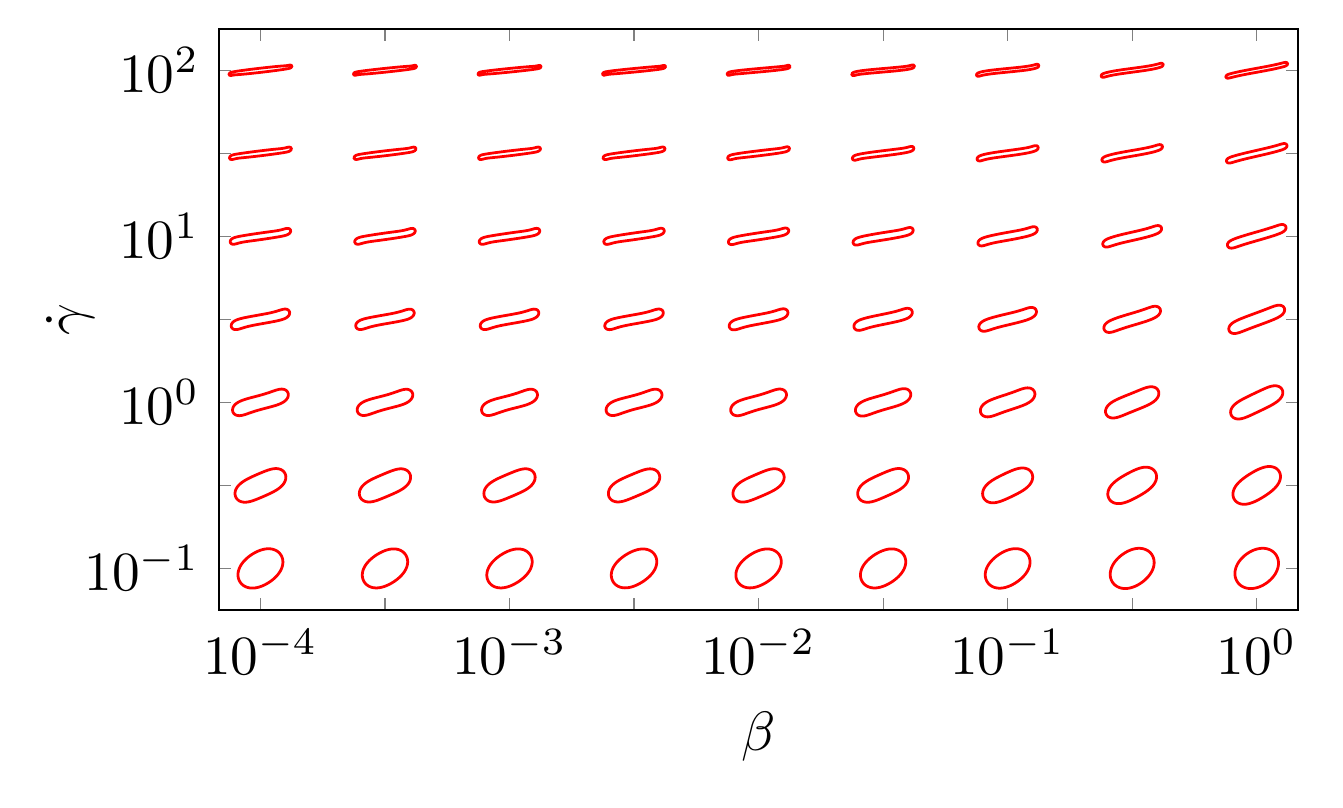
\begin{tikzpicture}[scale=2.0]

\pgfmathsetlengthmacro\MajorTickLength{
      \pgfkeysvalueof{/pgfplots/major tick length} * 0.5
    }

  \begin{axis}[
    major tick length=\MajorTickLength,
    compat=newest,
    axis equal image,
    xmin = 12,
    xmax = 64,
    ymin = 0,
    ymax = 28,
    xtick = {14,20,26,32,38,44,50,56,62},
    xticklabels = {$10^{-4}$,,$10^{-3}$,,$10^{-2}$,,
                    $10^{-1}$,,$10^{0}$},
    xlabel = {$\beta$},
    ytick = {2,6,10,14,18,22,26},
    yticklabels = {$10^{-1}$,,$10^{0}$,,$10^{1}$,,$10^2$},
    ylabel = {$\dot{\gamma}$},
    ylabel near ticks,
    ylabel shift = {-0.3cm},
  ]

%% beta = 1e-5,shear rate = 1e-1
%\addplot[red,line width=0.5pt] coordinates{
%(1.3082e+00,2.4832e+00)
%(1.2919e+00,2.4670e+00)
%(1.2754e+00,2.4502e+00)
%(1.2586e+00,2.4327e+00)
%(1.2413e+00,2.4139e+00)
%(1.2233e+00,2.3937e+00)
%(1.2044e+00,2.3719e+00)
%(1.1848e+00,2.3481e+00)
%(1.1643e+00,2.3223e+00)
%(1.1432e+00,2.2942e+00)
%(1.1215e+00,2.2638e+00)
%(1.0995e+00,2.2308e+00)
%(1.0773e+00,2.1952e+00)
%(1.0552e+00,2.1569e+00)
%(1.0337e+00,2.1158e+00)
%(1.0130e+00,2.0718e+00)
%(9.9361e-01,2.0249e+00)
%(9.7599e-01,1.9751e+00)
%(9.6068e-01,1.9226e+00)
%(9.4824e-01,1.8674e+00)
%(9.3928e-01,1.8097e+00)
%(9.3443e-01,1.7499e+00)
%(9.3429e-01,1.6884e+00)
%(9.3945e-01,1.6257e+00)
%(9.5045e-01,1.5624e+00)
%(9.6770e-01,1.4994e+00)
%(9.9148e-01,1.4374e+00)
%(1.0219e+00,1.3774e+00)
%(1.0589e+00,1.3204e+00)
%(1.1022e+00,1.2672e+00)
%(1.1513e+00,1.2186e+00)
%(1.2055e+00,1.1754e+00)
%(1.2640e+00,1.1380e+00)
%(1.3261e+00,1.1068e+00)
%(1.3908e+00,1.0818e+00)
%(1.4572e+00,1.0629e+00)
%(1.5246e+00,1.0500e+00)
%(1.5922e+00,1.0427e+00)
%(1.6594e+00,1.0405e+00)
%(1.7257e+00,1.0429e+00)
%(1.7908e+00,1.0495e+00)
%(1.8542e+00,1.0596e+00)
%(1.9158e+00,1.0729e+00)
%(1.9752e+00,1.0888e+00)
%(2.0324e+00,1.1068e+00)
%(2.0873e+00,1.1266e+00)
%(2.1398e+00,1.1478e+00)
%(2.1898e+00,1.1701e+00)
%(2.2373e+00,1.1931e+00)
%(2.2823e+00,1.2166e+00)
%(2.3248e+00,1.2402e+00)
%(2.3647e+00,1.2639e+00)
%(2.4022e+00,1.2873e+00)
%(2.4372e+00,1.3104e+00)
%(2.4699e+00,1.3329e+00)
%(2.5002e+00,1.3547e+00)
%(2.5283e+00,1.3758e+00)
%(2.5543e+00,1.3960e+00)
%(2.5783e+00,1.4154e+00)
%(2.6005e+00,1.4338e+00)
%(2.6210e+00,1.4515e+00)
%(2.6401e+00,1.4685e+00)
%(2.6581e+00,1.4848e+00)
%(2.6752e+00,1.5009e+00)
%(2.6918e+00,1.5168e+00)
%(2.7081e+00,1.5330e+00)
%(2.7246e+00,1.5498e+00)
%(2.7414e+00,1.5673e+00)
%(2.7587e+00,1.5861e+00)
%(2.7767e+00,1.6063e+00)
%(2.7956e+00,1.6281e+00)
%(2.8152e+00,1.6519e+00)
%(2.8357e+00,1.6777e+00)
%(2.8568e+00,1.7058e+00)
%(2.8785e+00,1.7362e+00)
%(2.9005e+00,1.7692e+00)
%(2.9227e+00,1.8048e+00)
%(2.9448e+00,1.8431e+00)
%(2.9663e+00,1.8842e+00)
%(2.9870e+00,1.9282e+00)
%(3.0064e+00,1.9751e+00)
%(3.0240e+00,2.0249e+00)
%(3.0393e+00,2.0774e+00)
%(3.0518e+00,2.1326e+00)
%(3.0607e+00,2.1903e+00)
%(3.0656e+00,2.2501e+00)
%(3.0657e+00,2.3116e+00)
%(3.0605e+00,2.3743e+00)
%(3.0496e+00,2.4376e+00)
%(3.0323e+00,2.5006e+00)
%(3.0085e+00,2.5626e+00)
%(2.9781e+00,2.6226e+00)
%(2.9411e+00,2.6796e+00)
%(2.8978e+00,2.7328e+00)
%(2.8487e+00,2.7814e+00)
%(2.7945e+00,2.8246e+00)
%(2.7360e+00,2.8620e+00)
%(2.6739e+00,2.8932e+00)
%(2.6092e+00,2.9182e+00)
%(2.5428e+00,2.9371e+00)
%(2.4754e+00,2.9500e+00)
%(2.4078e+00,2.9573e+00)
%(2.3406e+00,2.9595e+00)
%(2.2743e+00,2.9571e+00)
%(2.2092e+00,2.9505e+00)
%(2.1458e+00,2.9404e+00)
%(2.0842e+00,2.9271e+00)
%(2.0248e+00,2.9112e+00)
%(1.9676e+00,2.8932e+00)
%(1.9127e+00,2.8734e+00)
%(1.8602e+00,2.8522e+00)
%(1.8102e+00,2.8299e+00)
%(1.7627e+00,2.8069e+00)
%(1.7177e+00,2.7834e+00)
%(1.6752e+00,2.7598e+00)
%(1.6353e+00,2.7361e+00)
%(1.5978e+00,2.7127e+00)
%(1.5628e+00,2.6896e+00)
%(1.5301e+00,2.6671e+00)
%(1.4998e+00,2.6453e+00)
%(1.4717e+00,2.6242e+00)
%(1.4457e+00,2.6040e+00)
%(1.4217e+00,2.5846e+00)
%(1.3995e+00,2.5662e+00)
%(1.3790e+00,2.5485e+00)
%(1.3599e+00,2.5315e+00)
%(1.3419e+00,2.5152e+00)
%(1.3248e+00,2.4991e+00)
%(1.3082e+00,2.4832e+00)
%};
%
%% beta = 1e-5,shear rate = 1e-0.5
%\addplot[red,line width=0.5pt] coordinates{
%(2.5471e+00,6.8094e+00)
%(2.5246e+00,6.8052e+00)
%(2.5017e+00,6.8005e+00)
%(2.4780e+00,6.7951e+00)
%(2.4533e+00,6.7891e+00)
%(2.4272e+00,6.7823e+00)
%(2.3994e+00,6.7746e+00)
%(2.3700e+00,6.7658e+00)
%(2.3386e+00,6.7561e+00)
%(2.3054e+00,6.7451e+00)
%(2.2702e+00,6.7330e+00)
%(2.2329e+00,6.7196e+00)
%(2.1938e+00,6.7050e+00)
%(2.1526e+00,6.6891e+00)
%(2.1096e+00,6.6720e+00)
%(2.0647e+00,6.6537e+00)
%(2.0181e+00,6.6343e+00)
%(1.9697e+00,6.6136e+00)
%(1.9196e+00,6.5919e+00)
%(1.8680e+00,6.5690e+00)
%(1.8150e+00,6.5451e+00)
%(1.7606e+00,6.5202e+00)
%(1.7050e+00,6.4942e+00)
%(1.6484e+00,6.4671e+00)
%(1.5909e+00,6.4390e+00)
%(1.5327e+00,6.4096e+00)
%(1.4740e+00,6.3790e+00)
%(1.4150e+00,6.3470e+00)
%(1.3561e+00,6.3134e+00)
%(1.2974e+00,6.2782e+00)
%(1.2394e+00,6.2412e+00)
%(1.1824e+00,6.2020e+00)
%(1.1269e+00,6.1606e+00)
%(1.0733e+00,6.1166e+00)
%(1.0223e+00,6.0700e+00)
%(9.7444e-01,6.0205e+00)
%(9.3048e-01,5.9681e+00)
%(8.9122e-01,5.9129e+00)
%(8.5749e-01,5.8549e+00)
%(8.3016e-01,5.7946e+00)
%(8.1001e-01,5.7327e+00)
%(7.9770e-01,5.6699e+00)
%(7.9368e-01,5.6073e+00)
%(7.9806e-01,5.5462e+00)
%(8.1063e-01,5.4877e+00)
%(8.3076e-01,5.4332e+00)
%(8.5751e-01,5.3836e+00)
%(8.8969e-01,5.3395e+00)
%(9.2601e-01,5.3015e+00)
%(9.6514e-01,5.2695e+00)
%(1.0059e+00,5.2433e+00)
%(1.0472e+00,5.2224e+00)
%(1.0882e+00,5.2063e+00)
%(1.1282e+00,5.1943e+00)
%(1.1668e+00,5.1858e+00)
%(1.2037e+00,5.1801e+00)
%(1.2385e+00,5.1768e+00)
%(1.2713e+00,5.1753e+00)
%(1.3020e+00,5.1752e+00)
%(1.3308e+00,5.1762e+00)
%(1.3577e+00,5.1780e+00)
%(1.3831e+00,5.1805e+00)
%(1.4071e+00,5.1834e+00)
%(1.4303e+00,5.1868e+00)
%(1.4529e+00,5.1906e+00)
%(1.4754e+00,5.1948e+00)
%(1.4983e+00,5.1995e+00)
%(1.5220e+00,5.2049e+00)
%(1.5467e+00,5.2109e+00)
%(1.5728e+00,5.2177e+00)
%(1.6006e+00,5.2254e+00)
%(1.6300e+00,5.2342e+00)
%(1.6614e+00,5.2439e+00)
%(1.6946e+00,5.2549e+00)
%(1.7298e+00,5.2670e+00)
%(1.7671e+00,5.2804e+00)
%(1.8062e+00,5.2950e+00)
%(1.8474e+00,5.3109e+00)
%(1.8904e+00,5.3280e+00)
%(1.9353e+00,5.3463e+00)
%(1.9819e+00,5.3657e+00)
%(2.0303e+00,5.3864e+00)
%(2.0804e+00,5.4081e+00)
%(2.1320e+00,5.4310e+00)
%(2.1850e+00,5.4549e+00)
%(2.2394e+00,5.4798e+00)
%(2.2950e+00,5.5058e+00)
%(2.3516e+00,5.5329e+00)
%(2.4091e+00,5.5610e+00)
%(2.4673e+00,5.5904e+00)
%(2.5260e+00,5.6210e+00)
%(2.5850e+00,5.6530e+00)
%(2.6439e+00,5.6866e+00)
%(2.7026e+00,5.7218e+00)
%(2.7606e+00,5.7588e+00)
%(2.8176e+00,5.7980e+00)
%(2.8731e+00,5.8394e+00)
%(2.9267e+00,5.8834e+00)
%(2.9777e+00,5.9300e+00)
%(3.0256e+00,5.9795e+00)
%(3.0695e+00,6.0319e+00)
%(3.1088e+00,6.0871e+00)
%(3.1425e+00,6.1451e+00)
%(3.1698e+00,6.2054e+00)
%(3.1900e+00,6.2673e+00)
%(3.2023e+00,6.3301e+00)
%(3.2063e+00,6.3927e+00)
%(3.2019e+00,6.4538e+00)
%(3.1894e+00,6.5123e+00)
%(3.1692e+00,6.5668e+00)
%(3.1425e+00,6.6164e+00)
%(3.1103e+00,6.6605e+00)
%(3.0740e+00,6.6985e+00)
%(3.0349e+00,6.7305e+00)
%(2.9941e+00,6.7567e+00)
%(2.9528e+00,6.7776e+00)
%(2.9118e+00,6.7937e+00)
%(2.8718e+00,6.8057e+00)
%(2.8332e+00,6.8142e+00)
%(2.7963e+00,6.8199e+00)
%(2.7615e+00,6.8232e+00)
%(2.7287e+00,6.8247e+00)
%(2.6980e+00,6.8248e+00)
%(2.6692e+00,6.8238e+00)
%(2.6423e+00,6.8220e+00)
%(2.6169e+00,6.8195e+00)
%(2.5929e+00,6.8166e+00)
%(2.5697e+00,6.8132e+00)
%(2.5471e+00,6.8094e+00)
%};
%
%% beta = 1e-5,shear rate = 1e0
%\addplot[red,line width=0.5pt] coordinates{
%(7.4250e-01,9.8323e+00)
%(7.2969e-01,9.8134e+00)
%(7.1771e-01,9.7934e+00)
%(7.0652e-01,9.7720e+00)
%(6.9625e-01,9.7488e+00)
%(6.8719e-01,9.7235e+00)
%(6.7978e-01,9.6958e+00)
%(6.7465e-01,9.6656e+00)
%(6.7258e-01,9.6330e+00)
%(6.7446e-01,9.5982e+00)
%(6.8128e-01,9.5617e+00)
%(6.9398e-01,9.5245e+00)
%(7.1333e-01,9.4876e+00)
%(7.3977e-01,9.4527e+00)
%(7.7331e-01,9.4211e+00)
%(8.1347e-01,9.3944e+00)
%(8.5935e-01,9.3736e+00)
%(9.0980e-01,9.3596e+00)
%(9.6363e-01,9.3522e+00)
%(1.0198e+00,9.3513e+00)
%(1.0776e+00,9.3561e+00)
%(1.1364e+00,9.3658e+00)
%(1.1959e+00,9.3794e+00)
%(1.2562e+00,9.3960e+00)
%(1.3172e+00,9.4149e+00)
%(1.3788e+00,9.4352e+00)
%(1.4412e+00,9.4566e+00)
%(1.5044e+00,9.4784e+00)
%(1.5683e+00,9.5003e+00)
%(1.6329e+00,9.5222e+00)
%(1.6980e+00,9.5437e+00)
%(1.7636e+00,9.5648e+00)
%(1.8294e+00,9.5854e+00)
%(1.8955e+00,9.6055e+00)
%(1.9615e+00,9.6251e+00)
%(2.0274e+00,9.6442e+00)
%(2.0930e+00,9.6629e+00)
%(2.1580e+00,9.6812e+00)
%(2.2224e+00,9.6991e+00)
%(2.2859e+00,9.7167e+00)
%(2.3485e+00,9.7341e+00)
%(2.4099e+00,9.7513e+00)
%(2.4701e+00,9.7685e+00)
%(2.5288e+00,9.7855e+00)
%(2.5859e+00,9.8026e+00)
%(2.6412e+00,9.8197e+00)
%(2.6947e+00,9.8370e+00)
%(2.7462e+00,9.8545e+00)
%(2.7956e+00,9.8721e+00)
%(2.8427e+00,9.8901e+00)
%(2.8874e+00,9.9082e+00)
%(2.9297e+00,9.9267e+00)
%(2.9694e+00,9.9454e+00)
%(3.0066e+00,9.9642e+00)
%(3.0410e+00,9.9833e+00)
%(3.0729e+00,1.0002e+01)
%(3.1021e+00,1.0021e+01)
%(3.1288e+00,1.0040e+01)
%(3.1530e+00,1.0059e+01)
%(3.1749e+00,1.0077e+01)
%(3.1947e+00,1.0096e+01)
%(3.2126e+00,1.0114e+01)
%(3.2289e+00,1.0132e+01)
%(3.2438e+00,1.0149e+01)
%(3.2575e+00,1.0168e+01)
%(3.2703e+00,1.0187e+01)
%(3.2823e+00,1.0207e+01)
%(3.2935e+00,1.0228e+01)
%(3.3038e+00,1.0251e+01)
%(3.3128e+00,1.0277e+01)
%(3.3202e+00,1.0304e+01)
%(3.3253e+00,1.0334e+01)
%(3.3274e+00,1.0367e+01)
%(3.3255e+00,1.0402e+01)
%(3.3187e+00,1.0438e+01)
%(3.3060e+00,1.0476e+01)
%(3.2867e+00,1.0512e+01)
%(3.2602e+00,1.0547e+01)
%(3.2267e+00,1.0579e+01)
%(3.1865e+00,1.0606e+01)
%(3.1406e+00,1.0626e+01)
%(3.0902e+00,1.0640e+01)
%(3.0364e+00,1.0648e+01)
%(2.9802e+00,1.0649e+01)
%(2.9224e+00,1.0644e+01)
%(2.8636e+00,1.0634e+01)
%(2.8041e+00,1.0621e+01)
%(2.7438e+00,1.0604e+01)
%(2.6828e+00,1.0585e+01)
%(2.6212e+00,1.0565e+01)
%(2.5588e+00,1.0543e+01)
%(2.4956e+00,1.0522e+01)
%(2.4317e+00,1.0500e+01)
%(2.3671e+00,1.0478e+01)
%(2.3020e+00,1.0456e+01)
%(2.2364e+00,1.0435e+01)
%(2.1706e+00,1.0415e+01)
%(2.1045e+00,1.0394e+01)
%(2.0385e+00,1.0375e+01)
%(1.9726e+00,1.0356e+01)
%(1.9071e+00,1.0337e+01)
%(1.8420e+00,1.0319e+01)
%(1.7776e+00,1.0301e+01)
%(1.7141e+00,1.0283e+01)
%(1.6515e+00,1.0266e+01)
%(1.5901e+00,1.0249e+01)
%(1.5299e+00,1.0232e+01)
%(1.4712e+00,1.0214e+01)
%(1.4141e+00,1.0197e+01)
%(1.3588e+00,1.0180e+01)
%(1.3053e+00,1.0163e+01)
%(1.2538e+00,1.0146e+01)
%(1.2044e+00,1.0128e+01)
%(1.1573e+00,1.0110e+01)
%(1.1126e+00,1.0092e+01)
%(1.0703e+00,1.0073e+01)
%(1.0306e+00,1.0055e+01)
%(9.9345e-01,1.0036e+01)
%(9.5895e-01,1.0017e+01)
%(9.2710e-01,9.9977e+00)
%(8.9788e-01,9.9786e+00)
%(8.7120e-01,9.9597e+00)
%(8.4698e-01,9.9410e+00)
%(8.2507e-01,9.9225e+00)
%(8.0527e-01,9.9043e+00)
%(7.8737e-01,9.8863e+00)
%(7.7111e-01,9.8685e+00)
%(7.5623e-01,9.8505e+00)
%(7.4250e-01,9.8323e+00)
%};
%
%% beta = 1e-5,shear rate = 1e0.5
%\addplot[red,line width=0.5pt] coordinates{
%(1.3090e+00,1.3613e+01)
%(1.3310e+00,1.3619e+01)
%(1.3535e+00,1.3625e+01)
%(1.3769e+00,1.3631e+01)
%(1.4014e+00,1.3637e+01)
%(1.4275e+00,1.3644e+01)
%(1.4553e+00,1.3651e+01)
%(1.4851e+00,1.3658e+01)
%(1.5169e+00,1.3665e+01)
%(1.5509e+00,1.3673e+01)
%(1.5871e+00,1.3681e+01)
%(1.6256e+00,1.3689e+01)
%(1.6663e+00,1.3697e+01)
%(1.7092e+00,1.3706e+01)
%(1.7544e+00,1.3715e+01)
%(1.8017e+00,1.3724e+01)
%(1.8511e+00,1.3734e+01)
%(1.9025e+00,1.3744e+01)
%(1.9558e+00,1.3754e+01)
%(2.0109e+00,1.3765e+01)
%(2.0678e+00,1.3776e+01)
%(2.1262e+00,1.3787e+01)
%(2.1862e+00,1.3798e+01)
%(2.2475e+00,1.3810e+01)
%(2.3100e+00,1.3823e+01)
%(2.3736e+00,1.3835e+01)
%(2.4382e+00,1.3848e+01)
%(2.5036e+00,1.3861e+01)
%(2.5696e+00,1.3875e+01)
%(2.6362e+00,1.3889e+01)
%(2.7031e+00,1.3904e+01)
%(2.7702e+00,1.3919e+01)
%(2.8373e+00,1.3935e+01)
%(2.9041e+00,1.3952e+01)
%(2.9703e+00,1.3970e+01)
%(3.0357e+00,1.3991e+01)
%(3.0998e+00,1.4014e+01)
%(3.1620e+00,1.4040e+01)
%(3.2213e+00,1.4070e+01)
%(3.2763e+00,1.4106e+01)
%(3.3251e+00,1.4149e+01)
%(3.3648e+00,1.4199e+01)
%(3.3917e+00,1.4255e+01)
%(3.4021e+00,1.4315e+01)
%(3.3939e+00,1.4374e+01)
%(3.3679e+00,1.4425e+01)
%(3.3282e+00,1.4464e+01)
%(3.2806e+00,1.4490e+01)
%(3.2301e+00,1.4504e+01)
%(3.1800e+00,1.4508e+01)
%(3.1319e+00,1.4505e+01)
%(3.0863e+00,1.4498e+01)
%(3.0435e+00,1.4489e+01)
%(3.0032e+00,1.4479e+01)
%(2.9653e+00,1.4468e+01)
%(2.9298e+00,1.4458e+01)
%(2.8965e+00,1.4447e+01)
%(2.8652e+00,1.4438e+01)
%(2.8360e+00,1.4429e+01)
%(2.8086e+00,1.4421e+01)
%(2.7829e+00,1.4413e+01)
%(2.7585e+00,1.4406e+01)
%(2.7354e+00,1.4399e+01)
%(2.7130e+00,1.4393e+01)
%(2.6910e+00,1.4387e+01)
%(2.6690e+00,1.4381e+01)
%(2.6465e+00,1.4375e+01)
%(2.6231e+00,1.4369e+01)
%(2.5986e+00,1.4363e+01)
%(2.5725e+00,1.4356e+01)
%(2.5447e+00,1.4349e+01)
%(2.5149e+00,1.4342e+01)
%(2.4831e+00,1.4335e+01)
%(2.4491e+00,1.4327e+01)
%(2.4129e+00,1.4319e+01)
%(2.3744e+00,1.4311e+01)
%(2.3337e+00,1.4303e+01)
%(2.2908e+00,1.4294e+01)
%(2.2456e+00,1.4285e+01)
%(2.1983e+00,1.4276e+01)
%(2.1489e+00,1.4266e+01)
%(2.0975e+00,1.4256e+01)
%(2.0442e+00,1.4246e+01)
%(1.9891e+00,1.4235e+01)
%(1.9322e+00,1.4224e+01)
%(1.8738e+00,1.4213e+01)
%(1.8138e+00,1.4202e+01)
%(1.7525e+00,1.4190e+01)
%(1.6900e+00,1.4177e+01)
%(1.6264e+00,1.4165e+01)
%(1.5618e+00,1.4152e+01)
%(1.4964e+00,1.4139e+01)
%(1.4304e+00,1.4125e+01)
%(1.3638e+00,1.4111e+01)
%(1.2969e+00,1.4096e+01)
%(1.2298e+00,1.4081e+01)
%(1.1627e+00,1.4065e+01)
%(1.0959e+00,1.4048e+01)
%(1.0297e+00,1.4030e+01)
%(9.6426e-01,1.4009e+01)
%(9.0016e-01,1.3986e+01)
%(8.3801e-01,1.3960e+01)
%(7.7872e-01,1.3930e+01)
%(7.2367e-01,1.3894e+01)
%(6.7488e-01,1.3851e+01)
%(6.3523e-01,1.3801e+01)
%(6.0833e-01,1.3745e+01)
%(5.9787e-01,1.3685e+01)
%(6.0610e-01,1.3626e+01)
%(6.3214e-01,1.3575e+01)
%(6.7181e-01,1.3536e+01)
%(7.1940e-01,1.3510e+01)
%(7.6988e-01,1.3496e+01)
%(8.1999e-01,1.3492e+01)
%(8.6812e-01,1.3495e+01)
%(9.1367e-01,1.3502e+01)
%(9.5655e-01,1.3511e+01)
%(9.9684e-01,1.3521e+01)
%(1.0347e+00,1.3532e+01)
%(1.0702e+00,1.3542e+01)
%(1.1035e+00,1.3553e+01)
%(1.1348e+00,1.3562e+01)
%(1.1640e+00,1.3571e+01)
%(1.1914e+00,1.3579e+01)
%(1.2171e+00,1.3587e+01)
%(1.2415e+00,1.3594e+01)
%(1.2646e+00,1.3601e+01)
%(1.2870e+00,1.3607e+01)
%(1.3090e+00,1.3613e+01)
%};
%
%% beta = 1e-5,shear rate = 1e1
%\addplot[red,line width=0.5pt] coordinates{
%(2.3881e+00,1.7877e+01)
%(2.4105e+00,1.7881e+01)
%(2.4333e+00,1.7885e+01)
%(2.4570e+00,1.7890e+01)
%(2.4818e+00,1.7895e+01)
%(2.5082e+00,1.7900e+01)
%(2.5362e+00,1.7905e+01)
%(2.5662e+00,1.7911e+01)
%(2.5982e+00,1.7918e+01)
%(2.6323e+00,1.7925e+01)
%(2.6686e+00,1.7932e+01)
%(2.7071e+00,1.7940e+01)
%(2.7478e+00,1.7949e+01)
%(2.7906e+00,1.7958e+01)
%(2.8356e+00,1.7968e+01)
%(2.8827e+00,1.7978e+01)
%(2.9317e+00,1.7989e+01)
%(2.9826e+00,1.8001e+01)
%(3.0353e+00,1.8014e+01)
%(3.0896e+00,1.8028e+01)
%(3.1452e+00,1.8044e+01)
%(3.2018e+00,1.8063e+01)
%(3.2587e+00,1.8085e+01)
%(3.3147e+00,1.8112e+01)
%(3.3675e+00,1.8147e+01)
%(3.4125e+00,1.8194e+01)
%(3.4411e+00,1.8253e+01)
%(3.4419e+00,1.8319e+01)
%(3.4090e+00,1.8376e+01)
%(3.3511e+00,1.8411e+01)
%(3.2836e+00,1.8421e+01)
%(3.2152e+00,1.8415e+01)
%(3.1477e+00,1.8401e+01)
%(3.0808e+00,1.8384e+01)
%(3.0140e+00,1.8368e+01)
%(2.9472e+00,1.8353e+01)
%(2.8805e+00,1.8340e+01)
%(2.8142e+00,1.8328e+01)
%(2.7485e+00,1.8316e+01)
%(2.6835e+00,1.8306e+01)
%(2.6195e+00,1.8295e+01)
%(2.5566e+00,1.8285e+01)
%(2.4950e+00,1.8276e+01)
%(2.4347e+00,1.8266e+01)
%(2.3760e+00,1.8257e+01)
%(2.3189e+00,1.8248e+01)
%(2.2635e+00,1.8239e+01)
%(2.2099e+00,1.8230e+01)
%(2.1583e+00,1.8222e+01)
%(2.1088e+00,1.8213e+01)
%(2.0613e+00,1.8205e+01)
%(2.0159e+00,1.8197e+01)
%(1.9727e+00,1.8190e+01)
%(1.9318e+00,1.8182e+01)
%(1.8931e+00,1.8176e+01)
%(1.8566e+00,1.8169e+01)
%(1.8224e+00,1.8163e+01)
%(1.7903e+00,1.8157e+01)
%(1.7602e+00,1.8151e+01)
%(1.7321e+00,1.8146e+01)
%(1.7057e+00,1.8141e+01)
%(1.6808e+00,1.8137e+01)
%(1.6571e+00,1.8132e+01)
%(1.6343e+00,1.8128e+01)
%(1.6119e+00,1.8123e+01)
%(1.5895e+00,1.8119e+01)
%(1.5667e+00,1.8115e+01)
%(1.5430e+00,1.8110e+01)
%(1.5182e+00,1.8105e+01)
%(1.4918e+00,1.8100e+01)
%(1.4638e+00,1.8095e+01)
%(1.4338e+00,1.8089e+01)
%(1.4018e+00,1.8082e+01)
%(1.3677e+00,1.8075e+01)
%(1.3314e+00,1.8068e+01)
%(1.2929e+00,1.8060e+01)
%(1.2522e+00,1.8051e+01)
%(1.2094e+00,1.8042e+01)
%(1.1644e+00,1.8032e+01)
%(1.1173e+00,1.8022e+01)
%(1.0683e+00,1.8011e+01)
%(1.0174e+00,1.7999e+01)
%(9.6467e-01,1.7986e+01)
%(9.1039e-01,1.7972e+01)
%(8.5478e-01,1.7956e+01)
%(7.9822e-01,1.7937e+01)
%(7.4133e-01,1.7915e+01)
%(6.8532e-01,1.7888e+01)
%(6.3251e-01,1.7853e+01)
%(5.8755e-01,1.7806e+01)
%(5.5890e-01,1.7747e+01)
%(5.5806e-01,1.7681e+01)
%(5.9103e-01,1.7624e+01)
%(6.4895e-01,1.7589e+01)
%(7.1640e-01,1.7579e+01)
%(7.8479e-01,1.7585e+01)
%(8.5226e-01,1.7599e+01)
%(9.1921e-01,1.7616e+01)
%(9.8604e-01,1.7632e+01)
%(1.0528e+00,1.7647e+01)
%(1.1195e+00,1.7660e+01)
%(1.1858e+00,1.7672e+01)
%(1.2515e+00,1.7684e+01)
%(1.3165e+00,1.7694e+01)
%(1.3805e+00,1.7705e+01)
%(1.4434e+00,1.7715e+01)
%(1.5050e+00,1.7724e+01)
%(1.5653e+00,1.7734e+01)
%(1.6240e+00,1.7743e+01)
%(1.6811e+00,1.7752e+01)
%(1.7365e+00,1.7761e+01)
%(1.7901e+00,1.7770e+01)
%(1.8417e+00,1.7778e+01)
%(1.8912e+00,1.7787e+01)
%(1.9387e+00,1.7795e+01)
%(1.9841e+00,1.7803e+01)
%(2.0273e+00,1.7810e+01)
%(2.0682e+00,1.7818e+01)
%(2.1069e+00,1.7824e+01)
%(2.1434e+00,1.7831e+01)
%(2.1776e+00,1.7837e+01)
%(2.2097e+00,1.7843e+01)
%(2.2398e+00,1.7849e+01)
%(2.2679e+00,1.7854e+01)
%(2.2943e+00,1.7859e+01)
%(2.3192e+00,1.7863e+01)
%(2.3429e+00,1.7868e+01)
%(2.3657e+00,1.7872e+01)
%(2.3881e+00,1.7877e+01)
%};
%
%% beta = 1e-5,shear rate = 1e1.5
%\addplot[red,line width=0.5pt] coordinates{
%(3.3517e+00,2.2105e+01)
%(3.3727e+00,2.2114e+01)
%(3.3936e+00,2.2124e+01)
%(3.4143e+00,2.2136e+01)
%(3.4347e+00,2.2151e+01)
%(3.4539e+00,2.2170e+01)
%(3.4703e+00,2.2193e+01)
%(3.4812e+00,2.2222e+01)
%(3.4825e+00,2.2254e+01)
%(3.4705e+00,2.2287e+01)
%(3.4445e+00,2.2313e+01)
%(3.4084e+00,2.2328e+01)
%(3.3671e+00,2.2332e+01)
%(3.3235e+00,2.2328e+01)
%(3.2783e+00,2.2319e+01)
%(3.2311e+00,2.2309e+01)
%(3.1818e+00,2.2299e+01)
%(3.1303e+00,2.2290e+01)
%(3.0766e+00,2.2282e+01)
%(3.0210e+00,2.2275e+01)
%(2.9636e+00,2.2268e+01)
%(2.9044e+00,2.2261e+01)
%(2.8438e+00,2.2254e+01)
%(2.7818e+00,2.2247e+01)
%(2.7185e+00,2.2240e+01)
%(2.6541e+00,2.2232e+01)
%(2.5887e+00,2.2224e+01)
%(2.5226e+00,2.2216e+01)
%(2.4557e+00,2.2208e+01)
%(2.3882e+00,2.2199e+01)
%(2.3203e+00,2.2190e+01)
%(2.2522e+00,2.2180e+01)
%(2.1839e+00,2.2171e+01)
%(2.1157e+00,2.2161e+01)
%(2.0476e+00,2.2152e+01)
%(1.9799e+00,2.2142e+01)
%(1.9126e+00,2.2132e+01)
%(1.8459e+00,2.2122e+01)
%(1.7799e+00,2.2112e+01)
%(1.7149e+00,2.2102e+01)
%(1.6508e+00,2.2092e+01)
%(1.5879e+00,2.2082e+01)
%(1.5263e+00,2.2072e+01)
%(1.4661e+00,2.2062e+01)
%(1.4074e+00,2.2052e+01)
%(1.3503e+00,2.2042e+01)
%(1.2950e+00,2.2033e+01)
%(1.2415e+00,2.2024e+01)
%(1.1900e+00,2.2015e+01)
%(1.1405e+00,2.2006e+01)
%(1.0931e+00,2.1997e+01)
%(1.0478e+00,2.1989e+01)
%(1.0047e+00,2.1981e+01)
%(9.6388e-01,2.1973e+01)
%(9.2529e-01,2.1965e+01)
%(8.8896e-01,2.1958e+01)
%(8.5487e-01,2.1951e+01)
%(8.2295e-01,2.1944e+01)
%(7.9313e-01,2.1937e+01)
%(7.6529e-01,2.1931e+01)
%(7.3927e-01,2.1924e+01)
%(7.1484e-01,2.1917e+01)
%(6.9174e-01,2.1910e+01)
%(6.6967e-01,2.1903e+01)
%(6.4828e-01,2.1895e+01)
%(6.2728e-01,2.1886e+01)
%(6.0643e-01,2.1876e+01)
%(5.8570e-01,2.1864e+01)
%(5.6534e-01,2.1849e+01)
%(5.4613e-01,2.1830e+01)
%(5.2968e-01,2.1807e+01)
%(5.1882e-01,2.1778e+01)
%(5.1752e-01,2.1746e+01)
%(5.2953e-01,2.1713e+01)
%(5.5546e-01,2.1687e+01)
%(5.9156e-01,2.1672e+01)
%(6.3286e-01,2.1668e+01)
%(6.7647e-01,2.1672e+01)
%(7.2172e-01,2.1681e+01)
%(7.6887e-01,2.1691e+01)
%(8.1818e-01,2.1701e+01)
%(8.6971e-01,2.1710e+01)
%(9.2336e-01,2.1718e+01)
%(9.7900e-01,2.1725e+01)
%(1.0365e+00,2.1732e+01)
%(1.0956e+00,2.1739e+01)
%(1.1562e+00,2.1746e+01)
%(1.2182e+00,2.1753e+01)
%(1.2815e+00,2.1760e+01)
%(1.3459e+00,2.1768e+01)
%(1.4113e+00,2.1776e+01)
%(1.4775e+00,2.1784e+01)
%(1.5443e+00,2.1792e+01)
%(1.6118e+00,2.1801e+01)
%(1.6797e+00,2.1810e+01)
%(1.7478e+00,2.1820e+01)
%(1.8161e+00,2.1829e+01)
%(1.8843e+00,2.1839e+01)
%(1.9524e+00,2.1848e+01)
%(2.0201e+00,2.1858e+01)
%(2.0874e+00,2.1868e+01)
%(2.1541e+00,2.1878e+01)
%(2.2201e+00,2.1888e+01)
%(2.2851e+00,2.1898e+01)
%(2.3492e+00,2.1908e+01)
%(2.4121e+00,2.1918e+01)
%(2.4737e+00,2.1928e+01)
%(2.5339e+00,2.1938e+01)
%(2.5926e+00,2.1948e+01)
%(2.6497e+00,2.1958e+01)
%(2.7050e+00,2.1967e+01)
%(2.7585e+00,2.1976e+01)
%(2.8100e+00,2.1985e+01)
%(2.8595e+00,2.1994e+01)
%(2.9069e+00,2.2003e+01)
%(2.9522e+00,2.2011e+01)
%(2.9953e+00,2.2019e+01)
%(3.0361e+00,2.2027e+01)
%(3.0747e+00,2.2035e+01)
%(3.1110e+00,2.2042e+01)
%(3.1451e+00,2.2049e+01)
%(3.1771e+00,2.2056e+01)
%(3.2069e+00,2.2063e+01)
%(3.2347e+00,2.2069e+01)
%(3.2607e+00,2.2076e+01)
%(3.2852e+00,2.2083e+01)
%(3.3083e+00,2.2090e+01)
%(3.3303e+00,2.2097e+01)
%(3.3517e+00,2.2105e+01)
%};
%
%% beta = 1e-5,shear rate = 1e2
%\addplot[red,line width=0.5pt] coordinates{
%(1.1063e+00,2.5989e+01)
%(1.0841e+00,2.5984e+01)
%(1.0614e+00,2.5979e+01)
%(1.0381e+00,2.5974e+01)
%(1.0134e+00,2.5969e+01)
%(9.8737e-01,2.5963e+01)
%(9.5954e-01,2.5956e+01)
%(9.2996e-01,2.5950e+01)
%(8.9827e-01,2.5942e+01)
%(8.6465e-01,2.5934e+01)
%(8.2879e-01,2.5925e+01)
%(7.9097e-01,2.5915e+01)
%(7.5094e-01,2.5904e+01)
%(7.0915e-01,2.5892e+01)
%(6.6544e-01,2.5877e+01)
%(6.2084e-01,2.5860e+01)
%(5.7627e-01,2.5837e+01)
%(5.3697e-01,2.5803e+01)
%(5.1549e-01,2.5754e+01)
%(5.3367e-01,2.5704e+01)
%(5.8473e-01,2.5678e+01)
%(6.4358e-01,2.5675e+01)
%(7.0440e-01,2.5679e+01)
%(7.6628e-01,2.5683e+01)
%(8.2968e-01,2.5686e+01)
%(8.9395e-01,2.5691e+01)
%(9.5934e-01,2.5696e+01)
%(1.0253e+00,2.5703e+01)
%(1.0922e+00,2.5710e+01)
%(1.1593e+00,2.5717e+01)
%(1.2270e+00,2.5725e+01)
%(1.2948e+00,2.5734e+01)
%(1.3628e+00,2.5743e+01)
%(1.4307e+00,2.5752e+01)
%(1.4985e+00,2.5762e+01)
%(1.5658e+00,2.5772e+01)
%(1.6328e+00,2.5782e+01)
%(1.6990e+00,2.5792e+01)
%(1.7647e+00,2.5802e+01)
%(1.8293e+00,2.5813e+01)
%(1.8930e+00,2.5823e+01)
%(1.9555e+00,2.5833e+01)
%(2.0168e+00,2.5844e+01)
%(2.0767e+00,2.5854e+01)
%(2.1351e+00,2.5864e+01)
%(2.1918e+00,2.5874e+01)
%(2.2468e+00,2.5884e+01)
%(2.2999e+00,2.5894e+01)
%(2.3512e+00,2.5903e+01)
%(2.4005e+00,2.5912e+01)
%(2.4477e+00,2.5921e+01)
%(2.4927e+00,2.5930e+01)
%(2.5356e+00,2.5938e+01)
%(2.5762e+00,2.5946e+01)
%(2.6147e+00,2.5953e+01)
%(2.6509e+00,2.5960e+01)
%(2.6849e+00,2.5967e+01)
%(2.7167e+00,2.5974e+01)
%(2.7466e+00,2.5980e+01)
%(2.7745e+00,2.5985e+01)
%(2.8007e+00,2.5991e+01)
%(2.8253e+00,2.5996e+01)
%(2.8489e+00,2.6001e+01)
%(2.8715e+00,2.6006e+01)
%(2.8937e+00,2.6011e+01)
%(2.9159e+00,2.6016e+01)
%(2.9385e+00,2.6021e+01)
%(2.9619e+00,2.6026e+01)
%(2.9866e+00,2.6031e+01)
%(3.0126e+00,2.6037e+01)
%(3.0405e+00,2.6044e+01)
%(3.0700e+00,2.6050e+01)
%(3.1017e+00,2.6058e+01)
%(3.1353e+00,2.6066e+01)
%(3.1712e+00,2.6075e+01)
%(3.2090e+00,2.6085e+01)
%(3.2491e+00,2.6096e+01)
%(3.2908e+00,2.6108e+01)
%(3.3346e+00,2.6123e+01)
%(3.3792e+00,2.6140e+01)
%(3.4237e+00,2.6163e+01)
%(3.4630e+00,2.6197e+01)
%(3.4845e+00,2.6246e+01)
%(3.4663e+00,2.6296e+01)
%(3.4153e+00,2.6322e+01)
%(3.3564e+00,2.6325e+01)
%(3.2956e+00,2.6321e+01)
%(3.2337e+00,2.6317e+01)
%(3.1703e+00,2.6314e+01)
%(3.1061e+00,2.6309e+01)
%(3.0407e+00,2.6304e+01)
%(2.9747e+00,2.6297e+01)
%(2.9078e+00,2.6290e+01)
%(2.8407e+00,2.6283e+01)
%(2.7730e+00,2.6275e+01)
%(2.7052e+00,2.6266e+01)
%(2.6372e+00,2.6257e+01)
%(2.5693e+00,2.6248e+01)
%(2.5015e+00,2.6238e+01)
%(2.4342e+00,2.6228e+01)
%(2.3672e+00,2.6218e+01)
%(2.3010e+00,2.6208e+01)
%(2.2353e+00,2.6198e+01)
%(2.1707e+00,2.6187e+01)
%(2.1070e+00,2.6177e+01)
%(2.0445e+00,2.6167e+01)
%(1.9832e+00,2.6156e+01)
%(1.9233e+00,2.6146e+01)
%(1.8649e+00,2.6136e+01)
%(1.8082e+00,2.6126e+01)
%(1.7532e+00,2.6116e+01)
%(1.7001e+00,2.6106e+01)
%(1.6488e+00,2.6097e+01)
%(1.5995e+00,2.6088e+01)
%(1.5523e+00,2.6079e+01)
%(1.5073e+00,2.6070e+01)
%(1.4644e+00,2.6062e+01)
%(1.4238e+00,2.6054e+01)
%(1.3853e+00,2.6047e+01)
%(1.3491e+00,2.6040e+01)
%(1.3151e+00,2.6033e+01)
%(1.2833e+00,2.6026e+01)
%(1.2534e+00,2.6020e+01)
%(1.2255e+00,2.6015e+01)
%(1.1993e+00,2.6009e+01)
%(1.1747e+00,2.6004e+01)
%(1.1511e+00,2.5999e+01)
%(1.1285e+00,2.5994e+01)
%(1.1063e+00,2.5989e+01)
%};
%
%% beta = 1e-4.5,shear rate = 1e-1
%\addplot[red,line width=0.5pt] coordinates{
%(7.8403e+00,2.8763e+00)
%(7.8191e+00,2.8675e+00)
%(7.7976e+00,2.8581e+00)
%(7.7755e+00,2.8480e+00)
%(7.7524e+00,2.8370e+00)
%(7.7282e+00,2.8249e+00)
%(7.7026e+00,2.8116e+00)
%(7.6755e+00,2.7968e+00)
%(7.6469e+00,2.7805e+00)
%(7.6168e+00,2.7624e+00)
%(7.5852e+00,2.7425e+00)
%(7.5521e+00,2.7206e+00)
%(7.5177e+00,2.6966e+00)
%(7.4821e+00,2.6704e+00)
%(7.4455e+00,2.6418e+00)
%(7.4081e+00,2.6108e+00)
%(7.3700e+00,2.5772e+00)
%(7.3315e+00,2.5411e+00)
%(7.2929e+00,2.5023e+00)
%(7.2545e+00,2.4608e+00)
%(7.2165e+00,2.4165e+00)
%(7.1794e+00,2.3693e+00)
%(7.1434e+00,2.3194e+00)
%(7.1091e+00,2.2666e+00)
%(7.0768e+00,2.2111e+00)
%(7.0471e+00,2.1529e+00)
%(7.0203e+00,2.0921e+00)
%(6.9971e+00,2.0290e+00)
%(6.9780e+00,1.9637e+00)
%(6.9635e+00,1.8966e+00)
%(6.9541e+00,1.8282e+00)
%(6.9503e+00,1.7590e+00)
%(6.9524e+00,1.6895e+00)
%(6.9607e+00,1.6206e+00)
%(6.9754e+00,1.5528e+00)
%(6.9964e+00,1.4870e+00)
%(7.0236e+00,1.4241e+00)
%(7.0566e+00,1.3646e+00)
%(7.0949e+00,1.3094e+00)
%(7.1380e+00,1.2588e+00)
%(7.1850e+00,1.2134e+00)
%(7.2352e+00,1.1734e+00)
%(7.2877e+00,1.1387e+00)
%(7.3418e+00,1.1095e+00)
%(7.3968e+00,1.0854e+00)
%(7.4519e+00,1.0661e+00)
%(7.5065e+00,1.0514e+00)
%(7.5602e+00,1.0408e+00)
%(7.6125e+00,1.0338e+00)
%(7.6631e+00,1.0300e+00)
%(7.7117e+00,1.0289e+00)
%(7.7581e+00,1.0301e+00)
%(7.8022e+00,1.0332e+00)
%(7.8439e+00,1.0378e+00)
%(7.8831e+00,1.0437e+00)
%(7.9199e+00,1.0504e+00)
%(7.9542e+00,1.0578e+00)
%(7.9862e+00,1.0656e+00)
%(8.0159e+00,1.0737e+00)
%(8.0436e+00,1.0820e+00)
%(8.0694e+00,1.0902e+00)
%(8.0935e+00,1.0985e+00)
%(8.1164e+00,1.1067e+00)
%(8.1383e+00,1.1151e+00)
%(8.1597e+00,1.1237e+00)
%(8.1809e+00,1.1325e+00)
%(8.2024e+00,1.1419e+00)
%(8.2245e+00,1.1520e+00)
%(8.2476e+00,1.1630e+00)
%(8.2718e+00,1.1751e+00)
%(8.2974e+00,1.1884e+00)
%(8.3245e+00,1.2032e+00)
%(8.3531e+00,1.2195e+00)
%(8.3832e+00,1.2376e+00)
%(8.4148e+00,1.2575e+00)
%(8.4479e+00,1.2794e+00)
%(8.4823e+00,1.3034e+00)
%(8.5179e+00,1.3296e+00)
%(8.5545e+00,1.3582e+00)
%(8.5919e+00,1.3892e+00)
%(8.6300e+00,1.4228e+00)
%(8.6685e+00,1.4589e+00)
%(8.7071e+00,1.4977e+00)
%(8.7455e+00,1.5392e+00)
%(8.7835e+00,1.5835e+00)
%(8.8206e+00,1.6307e+00)
%(8.8566e+00,1.6806e+00)
%(8.8909e+00,1.7334e+00)
%(8.9232e+00,1.7889e+00)
%(8.9529e+00,1.8471e+00)
%(8.9797e+00,1.9079e+00)
%(9.0029e+00,1.9710e+00)
%(9.0220e+00,2.0363e+00)
%(9.0365e+00,2.1034e+00)
%(9.0459e+00,2.1718e+00)
%(9.0497e+00,2.2410e+00)
%(9.0476e+00,2.3105e+00)
%(9.0393e+00,2.3794e+00)
%(9.0246e+00,2.4472e+00)
%(9.0036e+00,2.5130e+00)
%(8.9764e+00,2.5759e+00)
%(8.9434e+00,2.6354e+00)
%(8.9051e+00,2.6906e+00)
%(8.8620e+00,2.7412e+00)
%(8.8150e+00,2.7866e+00)
%(8.7648e+00,2.8266e+00)
%(8.7123e+00,2.8613e+00)
%(8.6582e+00,2.8905e+00)
%(8.6032e+00,2.9146e+00)
%(8.5481e+00,2.9339e+00)
%(8.4935e+00,2.9486e+00)
%(8.4398e+00,2.9592e+00)
%(8.3875e+00,2.9662e+00)
%(8.3369e+00,2.9700e+00)
%(8.2883e+00,2.9711e+00)
%(8.2419e+00,2.9699e+00)
%(8.1978e+00,2.9668e+00)
%(8.1561e+00,2.9622e+00)
%(8.1169e+00,2.9563e+00)
%(8.0801e+00,2.9496e+00)
%(8.0458e+00,2.9422e+00)
%(8.0138e+00,2.9344e+00)
%(7.9841e+00,2.9263e+00)
%(7.9564e+00,2.9180e+00)
%(7.9306e+00,2.9098e+00)
%(7.9065e+00,2.9015e+00)
%(7.8836e+00,2.8933e+00)
%(7.8617e+00,2.8849e+00)
%(7.8403e+00,2.8763e+00)
%};
%
%% beta = 1e-4.5,shear rate = 1e-0.5
%\addplot[red,line width=0.5pt] coordinates{
%(6.8580e+00,5.8393e+00)
%(6.8488e+00,5.8182e+00)
%(6.8402e+00,5.7963e+00)
%(6.8322e+00,5.7734e+00)
%(6.8248e+00,5.7490e+00)
%(6.8181e+00,5.7227e+00)
%(6.8124e+00,5.6944e+00)
%(6.8081e+00,5.6639e+00)
%(6.8055e+00,5.6311e+00)
%(6.8052e+00,5.5960e+00)
%(6.8077e+00,5.5587e+00)
%(6.8136e+00,5.5195e+00)
%(6.8237e+00,5.4788e+00)
%(6.8386e+00,5.4372e+00)
%(6.8587e+00,5.3954e+00)
%(6.8846e+00,5.3542e+00)
%(6.9165e+00,5.3148e+00)
%(6.9543e+00,5.2780e+00)
%(6.9979e+00,5.2450e+00)
%(7.0468e+00,5.2165e+00)
%(7.1002e+00,5.1932e+00)
%(7.1576e+00,5.1756e+00)
%(7.2179e+00,5.1638e+00)
%(7.2806e+00,5.1576e+00)
%(7.3448e+00,5.1569e+00)
%(7.4100e+00,5.1612e+00)
%(7.4758e+00,5.1700e+00)
%(7.5419e+00,5.1826e+00)
%(7.6080e+00,5.1986e+00)
%(7.6740e+00,5.2174e+00)
%(7.7398e+00,5.2385e+00)
%(7.8052e+00,5.2615e+00)
%(7.8703e+00,5.2860e+00)
%(7.9348e+00,5.3117e+00)
%(7.9988e+00,5.3384e+00)
%(8.0622e+00,5.3658e+00)
%(8.1248e+00,5.3939e+00)
%(8.1866e+00,5.4224e+00)
%(8.2474e+00,5.4512e+00)
%(8.3071e+00,5.4804e+00)
%(8.3655e+00,5.5098e+00)
%(8.4225e+00,5.5394e+00)
%(8.4779e+00,5.5692e+00)
%(8.5317e+00,5.5991e+00)
%(8.5836e+00,5.6292e+00)
%(8.6336e+00,5.6593e+00)
%(8.6815e+00,5.6895e+00)
%(8.7271e+00,5.7198e+00)
%(8.7703e+00,5.7500e+00)
%(8.8112e+00,5.7801e+00)
%(8.8495e+00,5.8100e+00)
%(8.8853e+00,5.8397e+00)
%(8.9184e+00,5.8689e+00)
%(8.9490e+00,5.8977e+00)
%(8.9769e+00,5.9258e+00)
%(9.0024e+00,5.9531e+00)
%(9.0254e+00,5.9797e+00)
%(9.0461e+00,6.0052e+00)
%(9.0647e+00,6.0298e+00)
%(9.0813e+00,6.0535e+00)
%(9.0961e+00,6.0761e+00)
%(9.1094e+00,6.0980e+00)
%(9.1213e+00,6.1192e+00)
%(9.1321e+00,6.1400e+00)
%(9.1420e+00,6.1607e+00)
%(9.1512e+00,6.1818e+00)
%(9.1598e+00,6.2037e+00)
%(9.1678e+00,6.2266e+00)
%(9.1752e+00,6.2510e+00)
%(9.1819e+00,6.2773e+00)
%(9.1876e+00,6.3056e+00)
%(9.1919e+00,6.3361e+00)
%(9.1945e+00,6.3689e+00)
%(9.1948e+00,6.4040e+00)
%(9.1923e+00,6.4413e+00)
%(9.1864e+00,6.4805e+00)
%(9.1763e+00,6.5212e+00)
%(9.1614e+00,6.5628e+00)
%(9.1413e+00,6.6046e+00)
%(9.1154e+00,6.6458e+00)
%(9.0835e+00,6.6852e+00)
%(9.0457e+00,6.7220e+00)
%(9.0021e+00,6.7550e+00)
%(8.9532e+00,6.7835e+00)
%(8.8998e+00,6.8068e+00)
%(8.8424e+00,6.8244e+00)
%(8.7821e+00,6.8362e+00)
%(8.7194e+00,6.8424e+00)
%(8.6552e+00,6.8431e+00)
%(8.5900e+00,6.8388e+00)
%(8.5242e+00,6.8300e+00)
%(8.4581e+00,6.8174e+00)
%(8.3920e+00,6.8014e+00)
%(8.3260e+00,6.7826e+00)
%(8.2602e+00,6.7615e+00)
%(8.1948e+00,6.7385e+00)
%(8.1297e+00,6.7140e+00)
%(8.0652e+00,6.6883e+00)
%(8.0012e+00,6.6616e+00)
%(7.9378e+00,6.6342e+00)
%(7.8752e+00,6.6061e+00)
%(7.8134e+00,6.5776e+00)
%(7.7526e+00,6.5488e+00)
%(7.6929e+00,6.5196e+00)
%(7.6345e+00,6.4902e+00)
%(7.5775e+00,6.4606e+00)
%(7.5221e+00,6.4308e+00)
%(7.4683e+00,6.4009e+00)
%(7.4164e+00,6.3708e+00)
%(7.3664e+00,6.3407e+00)
%(7.3185e+00,6.3105e+00)
%(7.2729e+00,6.2802e+00)
%(7.2297e+00,6.2500e+00)
%(7.1888e+00,6.2199e+00)
%(7.1505e+00,6.1900e+00)
%(7.1147e+00,6.1603e+00)
%(7.0816e+00,6.1311e+00)
%(7.0510e+00,6.1023e+00)
%(7.0231e+00,6.0742e+00)
%(6.9976e+00,6.0469e+00)
%(6.9746e+00,6.0203e+00)
%(6.9539e+00,5.9948e+00)
%(6.9353e+00,5.9702e+00)
%(6.9187e+00,5.9465e+00)
%(6.9039e+00,5.9239e+00)
%(6.8906e+00,5.9020e+00)
%(6.8787e+00,5.8808e+00)
%(6.8679e+00,5.8600e+00)
%(6.8580e+00,5.8393e+00)
%};
%
%% beta = 1e-4.5,shear rate = 1e0
%\addplot[red,line width=0.5pt] coordinates{
%(8.4228e+00,1.0516e+01)
%(8.4011e+00,1.0509e+01)
%(8.3789e+00,1.0502e+01)
%(8.3559e+00,1.0494e+01)
%(8.3317e+00,1.0486e+01)
%(8.3060e+00,1.0478e+01)
%(8.2786e+00,1.0469e+01)
%(8.2493e+00,1.0459e+01)
%(8.2180e+00,1.0449e+01)
%(8.1846e+00,1.0439e+01)
%(8.1490e+00,1.0427e+01)
%(8.1112e+00,1.0416e+01)
%(8.0712e+00,1.0404e+01)
%(8.0289e+00,1.0391e+01)
%(7.9846e+00,1.0377e+01)
%(7.9380e+00,1.0364e+01)
%(7.8895e+00,1.0349e+01)
%(7.8389e+00,1.0335e+01)
%(7.7865e+00,1.0319e+01)
%(7.7323e+00,1.0303e+01)
%(7.6764e+00,1.0287e+01)
%(7.6190e+00,1.0270e+01)
%(7.5601e+00,1.0252e+01)
%(7.5001e+00,1.0234e+01)
%(7.4389e+00,1.0215e+01)
%(7.3768e+00,1.0195e+01)
%(7.3141e+00,1.0173e+01)
%(7.2509e+00,1.0151e+01)
%(7.1875e+00,1.0126e+01)
%(7.1242e+00,1.0100e+01)
%(7.0615e+00,1.0071e+01)
%(6.9999e+00,1.0040e+01)
%(6.9399e+00,1.0005e+01)
%(6.8824e+00,9.9664e+00)
%(6.8285e+00,9.9230e+00)
%(6.7795e+00,9.8746e+00)
%(6.7373e+00,9.8208e+00)
%(6.7038e+00,9.7618e+00)
%(6.6814e+00,9.6986e+00)
%(6.6721e+00,9.6331e+00)
%(6.6773e+00,9.5682e+00)
%(6.6970e+00,9.5074e+00)
%(6.7299e+00,9.4540e+00)
%(6.7731e+00,9.4105e+00)
%(6.8232e+00,9.3779e+00)
%(6.8770e+00,9.3559e+00)
%(6.9320e+00,9.3431e+00)
%(6.9864e+00,9.3379e+00)
%(7.0390e+00,9.3384e+00)
%(7.0894e+00,9.3430e+00)
%(7.1373e+00,9.3506e+00)
%(7.1827e+00,9.3601e+00)
%(7.2255e+00,9.3706e+00)
%(7.2659e+00,9.3817e+00)
%(7.3038e+00,9.3930e+00)
%(7.3395e+00,9.4041e+00)
%(7.3728e+00,9.4148e+00)
%(7.4040e+00,9.4251e+00)
%(7.4332e+00,9.4348e+00)
%(7.4605e+00,9.4440e+00)
%(7.4861e+00,9.4527e+00)
%(7.5103e+00,9.4609e+00)
%(7.5332e+00,9.4687e+00)
%(7.5554e+00,9.4762e+00)
%(7.5772e+00,9.4835e+00)
%(7.5989e+00,9.4908e+00)
%(7.6211e+00,9.4983e+00)
%(7.6441e+00,9.5059e+00)
%(7.6683e+00,9.5140e+00)
%(7.6940e+00,9.5224e+00)
%(7.7214e+00,9.5313e+00)
%(7.7507e+00,9.5408e+00)
%(7.7820e+00,9.5508e+00)
%(7.8154e+00,9.5614e+00)
%(7.8510e+00,9.5725e+00)
%(7.8888e+00,9.5842e+00)
%(7.9288e+00,9.5965e+00)
%(7.9711e+00,9.6092e+00)
%(8.0154e+00,9.6225e+00)
%(8.0620e+00,9.6364e+00)
%(8.1105e+00,9.6507e+00)
%(8.1611e+00,9.6655e+00)
%(8.2135e+00,9.6808e+00)
%(8.2677e+00,9.6966e+00)
%(8.3236e+00,9.7130e+00)
%(8.3810e+00,9.7300e+00)
%(8.4399e+00,9.7477e+00)
%(8.4999e+00,9.7660e+00)
%(8.5611e+00,9.7852e+00)
%(8.6232e+00,9.8054e+00)
%(8.6859e+00,9.8267e+00)
%(8.7491e+00,9.8494e+00)
%(8.8125e+00,9.8737e+00)
%(8.8758e+00,9.8999e+00)
%(8.9385e+00,9.9285e+00)
%(9.0001e+00,9.9600e+00)
%(9.0601e+00,9.9948e+00)
%(9.1176e+00,1.0034e+01)
%(9.1715e+00,1.0077e+01)
%(9.2205e+00,1.0125e+01)
%(9.2627e+00,1.0179e+01)
%(9.2962e+00,1.0238e+01)
%(9.3186e+00,1.0301e+01)
%(9.3279e+00,1.0367e+01)
%(9.3227e+00,1.0432e+01)
%(9.3030e+00,1.0493e+01)
%(9.2701e+00,1.0546e+01)
%(9.2269e+00,1.0589e+01)
%(9.1768e+00,1.0622e+01)
%(9.1230e+00,1.0644e+01)
%(9.0680e+00,1.0657e+01)
%(9.0136e+00,1.0662e+01)
%(8.9610e+00,1.0662e+01)
%(8.9106e+00,1.0657e+01)
%(8.8627e+00,1.0649e+01)
%(8.8173e+00,1.0640e+01)
%(8.7745e+00,1.0629e+01)
%(8.7341e+00,1.0618e+01)
%(8.6962e+00,1.0607e+01)
%(8.6605e+00,1.0596e+01)
%(8.6272e+00,1.0585e+01)
%(8.5960e+00,1.0575e+01)
%(8.5668e+00,1.0565e+01)
%(8.5395e+00,1.0556e+01)
%(8.5139e+00,1.0547e+01)
%(8.4897e+00,1.0539e+01)
%(8.4668e+00,1.0531e+01)
%(8.4446e+00,1.0524e+01)
%(8.4228e+00,1.0516e+01)
%};
%
%% beta = 1e-4.5,shear rate = 1e0.5
%\addplot[red,line width=0.5pt] coordinates{
%(8.9402e+00,1.4456e+01)
%(8.9183e+00,1.4449e+01)
%(8.8960e+00,1.4442e+01)
%(8.8729e+00,1.4435e+01)
%(8.8486e+00,1.4427e+01)
%(8.8228e+00,1.4420e+01)
%(8.7953e+00,1.4411e+01)
%(8.7658e+00,1.4403e+01)
%(8.7343e+00,1.4394e+01)
%(8.7007e+00,1.4384e+01)
%(8.6647e+00,1.4375e+01)
%(8.6265e+00,1.4365e+01)
%(8.5860e+00,1.4354e+01)
%(8.5433e+00,1.4344e+01)
%(8.4982e+00,1.4334e+01)
%(8.4510e+00,1.4323e+01)
%(8.4016e+00,1.4312e+01)
%(8.3502e+00,1.4302e+01)
%(8.2968e+00,1.4291e+01)
%(8.2415e+00,1.4280e+01)
%(8.1845e+00,1.4269e+01)
%(8.1258e+00,1.4258e+01)
%(8.0656e+00,1.4246e+01)
%(8.0040e+00,1.4235e+01)
%(7.9412e+00,1.4223e+01)
%(7.8772e+00,1.4211e+01)
%(7.8123e+00,1.4199e+01)
%(7.7465e+00,1.4186e+01)
%(7.6800e+00,1.4173e+01)
%(7.6129e+00,1.4160e+01)
%(7.5454e+00,1.4147e+01)
%(7.4777e+00,1.4134e+01)
%(7.4099e+00,1.4120e+01)
%(7.3422e+00,1.4106e+01)
%(7.2747e+00,1.4091e+01)
%(7.2076e+00,1.4076e+01)
%(7.1412e+00,1.4060e+01)
%(7.0756e+00,1.4044e+01)
%(7.0111e+00,1.4026e+01)
%(6.9480e+00,1.4006e+01)
%(6.8867e+00,1.3984e+01)
%(6.8278e+00,1.3959e+01)
%(6.7721e+00,1.3930e+01)
%(6.7206e+00,1.3897e+01)
%(6.6749e+00,1.3859e+01)
%(6.6369e+00,1.3815e+01)
%(6.6090e+00,1.3766e+01)
%(6.5935e+00,1.3714e+01)
%(6.5921e+00,1.3662e+01)
%(6.6048e+00,1.3613e+01)
%(6.6294e+00,1.3571e+01)
%(6.6625e+00,1.3539e+01)
%(6.7003e+00,1.3517e+01)
%(6.7397e+00,1.3503e+01)
%(6.7785e+00,1.3496e+01)
%(6.8157e+00,1.3495e+01)
%(6.8506e+00,1.3496e+01)
%(6.8831e+00,1.3500e+01)
%(6.9133e+00,1.3505e+01)
%(6.9414e+00,1.3512e+01)
%(6.9676e+00,1.3518e+01)
%(6.9922e+00,1.3525e+01)
%(7.0154e+00,1.3531e+01)
%(7.0378e+00,1.3538e+01)
%(7.0598e+00,1.3544e+01)
%(7.0817e+00,1.3551e+01)
%(7.1040e+00,1.3558e+01)
%(7.1271e+00,1.3565e+01)
%(7.1514e+00,1.3573e+01)
%(7.1772e+00,1.3580e+01)
%(7.2047e+00,1.3589e+01)
%(7.2342e+00,1.3597e+01)
%(7.2657e+00,1.3606e+01)
%(7.2993e+00,1.3616e+01)
%(7.3353e+00,1.3625e+01)
%(7.3735e+00,1.3635e+01)
%(7.4140e+00,1.3646e+01)
%(7.4567e+00,1.3656e+01)
%(7.5018e+00,1.3666e+01)
%(7.5490e+00,1.3677e+01)
%(7.5984e+00,1.3688e+01)
%(7.6498e+00,1.3698e+01)
%(7.7032e+00,1.3709e+01)
%(7.7585e+00,1.3720e+01)
%(7.8155e+00,1.3731e+01)
%(7.8742e+00,1.3742e+01)
%(7.9344e+00,1.3754e+01)
%(7.9960e+00,1.3765e+01)
%(8.0588e+00,1.3777e+01)
%(8.1228e+00,1.3789e+01)
%(8.1877e+00,1.3801e+01)
%(8.2535e+00,1.3814e+01)
%(8.3200e+00,1.3827e+01)
%(8.3871e+00,1.3840e+01)
%(8.4546e+00,1.3853e+01)
%(8.5223e+00,1.3866e+01)
%(8.5901e+00,1.3880e+01)
%(8.6578e+00,1.3894e+01)
%(8.7253e+00,1.3909e+01)
%(8.7924e+00,1.3924e+01)
%(8.8588e+00,1.3940e+01)
%(8.9244e+00,1.3956e+01)
%(8.9889e+00,1.3974e+01)
%(9.0520e+00,1.3994e+01)
%(9.1133e+00,1.4016e+01)
%(9.1722e+00,1.4041e+01)
%(9.2279e+00,1.4070e+01)
%(9.2794e+00,1.4103e+01)
%(9.3251e+00,1.4141e+01)
%(9.3631e+00,1.4185e+01)
%(9.3910e+00,1.4234e+01)
%(9.4065e+00,1.4286e+01)
%(9.4079e+00,1.4338e+01)
%(9.3952e+00,1.4387e+01)
%(9.3706e+00,1.4429e+01)
%(9.3375e+00,1.4461e+01)
%(9.2997e+00,1.4483e+01)
%(9.2603e+00,1.4497e+01)
%(9.2215e+00,1.4504e+01)
%(9.1843e+00,1.4505e+01)
%(9.1494e+00,1.4504e+01)
%(9.1169e+00,1.4500e+01)
%(9.0867e+00,1.4495e+01)
%(9.0586e+00,1.4488e+01)
%(9.0324e+00,1.4482e+01)
%(9.0078e+00,1.4475e+01)
%(8.9846e+00,1.4469e+01)
%(8.9622e+00,1.4462e+01)
%(8.9402e+00,1.4456e+01)
%};
%
%% beta = 1e-4.5,shear rate = 1e1
%\addplot[red,line width=0.5pt] coordinates{
%(7.3554e+00,1.7747e+01)
%(7.3781e+00,1.7751e+01)
%(7.4011e+00,1.7754e+01)
%(7.4250e+00,1.7757e+01)
%(7.4501e+00,1.7761e+01)
%(7.4768e+00,1.7764e+01)
%(7.5052e+00,1.7768e+01)
%(7.5355e+00,1.7772e+01)
%(7.5679e+00,1.7777e+01)
%(7.6024e+00,1.7782e+01)
%(7.6392e+00,1.7786e+01)
%(7.6782e+00,1.7792e+01)
%(7.7195e+00,1.7797e+01)
%(7.7630e+00,1.7803e+01)
%(7.8086e+00,1.7810e+01)
%(7.8564e+00,1.7816e+01)
%(7.9063e+00,1.7824e+01)
%(7.9582e+00,1.7831e+01)
%(8.0120e+00,1.7839e+01)
%(8.0675e+00,1.7847e+01)
%(8.1249e+00,1.7855e+01)
%(8.1838e+00,1.7864e+01)
%(8.2442e+00,1.7873e+01)
%(8.3060e+00,1.7883e+01)
%(8.3690e+00,1.7893e+01)
%(8.4331e+00,1.7903e+01)
%(8.4982e+00,1.7913e+01)
%(8.5641e+00,1.7924e+01)
%(8.6308e+00,1.7935e+01)
%(8.6980e+00,1.7946e+01)
%(8.7656e+00,1.7957e+01)
%(8.8334e+00,1.7969e+01)
%(8.9014e+00,1.7981e+01)
%(8.9692e+00,1.7994e+01)
%(9.0368e+00,1.8007e+01)
%(9.1039e+00,1.8021e+01)
%(9.1701e+00,1.8037e+01)
%(9.2349e+00,1.8056e+01)
%(9.2974e+00,1.8080e+01)
%(9.3557e+00,1.8110e+01)
%(9.4065e+00,1.8150e+01)
%(9.4435e+00,1.8202e+01)
%(9.4578e+00,1.8262e+01)
%(9.4427e+00,1.8321e+01)
%(9.4020e+00,1.8363e+01)
%(9.3484e+00,1.8384e+01)
%(9.2925e+00,1.8388e+01)
%(9.2386e+00,1.8381e+01)
%(9.1876e+00,1.8369e+01)
%(9.1390e+00,1.8356e+01)
%(9.0926e+00,1.8343e+01)
%(9.0481e+00,1.8331e+01)
%(9.0056e+00,1.8320e+01)
%(8.9652e+00,1.8310e+01)
%(8.9268e+00,1.8301e+01)
%(8.8904e+00,1.8294e+01)
%(8.8562e+00,1.8287e+01)
%(8.8241e+00,1.8281e+01)
%(8.7939e+00,1.8276e+01)
%(8.7657e+00,1.8271e+01)
%(8.7391e+00,1.8267e+01)
%(8.7141e+00,1.8263e+01)
%(8.6902e+00,1.8259e+01)
%(8.6672e+00,1.8256e+01)
%(8.6446e+00,1.8253e+01)
%(8.6219e+00,1.8249e+01)
%(8.5989e+00,1.8246e+01)
%(8.5750e+00,1.8243e+01)
%(8.5499e+00,1.8239e+01)
%(8.5232e+00,1.8236e+01)
%(8.4948e+00,1.8232e+01)
%(8.4645e+00,1.8228e+01)
%(8.4321e+00,1.8223e+01)
%(8.3976e+00,1.8218e+01)
%(8.3608e+00,1.8214e+01)
%(8.3218e+00,1.8208e+01)
%(8.2805e+00,1.8203e+01)
%(8.2370e+00,1.8197e+01)
%(8.1914e+00,1.8190e+01)
%(8.1436e+00,1.8184e+01)
%(8.0937e+00,1.8176e+01)
%(8.0418e+00,1.8169e+01)
%(7.9880e+00,1.8161e+01)
%(7.9324e+00,1.8153e+01)
%(7.8751e+00,1.8145e+01)
%(7.8162e+00,1.8136e+01)
%(7.7558e+00,1.8127e+01)
%(7.6940e+00,1.8117e+01)
%(7.6310e+00,1.8107e+01)
%(7.5669e+00,1.8097e+01)
%(7.5018e+00,1.8087e+01)
%(7.4359e+00,1.8076e+01)
%(7.3692e+00,1.8065e+01)
%(7.3020e+00,1.8054e+01)
%(7.2344e+00,1.8043e+01)
%(7.1666e+00,1.8031e+01)
%(7.0986e+00,1.8019e+01)
%(7.0308e+00,1.8006e+01)
%(6.9632e+00,1.7993e+01)
%(6.8961e+00,1.7979e+01)
%(6.8299e+00,1.7963e+01)
%(6.7651e+00,1.7944e+01)
%(6.7026e+00,1.7920e+01)
%(6.6443e+00,1.7890e+01)
%(6.5935e+00,1.7850e+01)
%(6.5565e+00,1.7798e+01)
%(6.5422e+00,1.7738e+01)
%(6.5573e+00,1.7679e+01)
%(6.5980e+00,1.7637e+01)
%(6.6516e+00,1.7616e+01)
%(6.7075e+00,1.7612e+01)
%(6.7614e+00,1.7619e+01)
%(6.8124e+00,1.7631e+01)
%(6.8610e+00,1.7644e+01)
%(6.9074e+00,1.7657e+01)
%(6.9519e+00,1.7669e+01)
%(6.9944e+00,1.7680e+01)
%(7.0348e+00,1.7690e+01)
%(7.0732e+00,1.7699e+01)
%(7.1096e+00,1.7706e+01)
%(7.1438e+00,1.7713e+01)
%(7.1759e+00,1.7719e+01)
%(7.2061e+00,1.7724e+01)
%(7.2343e+00,1.7729e+01)
%(7.2609e+00,1.7733e+01)
%(7.2859e+00,1.7737e+01)
%(7.3098e+00,1.7741e+01)
%(7.3328e+00,1.7744e+01)
%(7.3554e+00,1.7747e+01)
%};
%
%% beta = 1e-4.5,shear rate = 1e1.5
%\addplot[red,line width=0.5pt] coordinates{
%(6.7048e+00,2.1930e+01)
%(6.6828e+00,2.1924e+01)
%(6.6605e+00,2.1918e+01)
%(6.6377e+00,2.1910e+01)
%(6.6142e+00,2.1900e+01)
%(6.5901e+00,2.1889e+01)
%(6.5659e+00,2.1873e+01)
%(6.5429e+00,2.1853e+01)
%(6.5233e+00,2.1827e+01)
%(6.5116e+00,2.1795e+01)
%(6.5134e+00,2.1758e+01)
%(6.5329e+00,2.1724e+01)
%(6.5676e+00,2.1702e+01)
%(6.6106e+00,2.1695e+01)
%(6.6564e+00,2.1698e+01)
%(6.7036e+00,2.1708e+01)
%(6.7523e+00,2.1721e+01)
%(6.8032e+00,2.1733e+01)
%(6.8564e+00,2.1744e+01)
%(6.9117e+00,2.1753e+01)
%(6.9690e+00,2.1761e+01)
%(7.0280e+00,2.1769e+01)
%(7.0887e+00,2.1775e+01)
%(7.1508e+00,2.1782e+01)
%(7.2142e+00,2.1788e+01)
%(7.2787e+00,2.1794e+01)
%(7.3442e+00,2.1801e+01)
%(7.4105e+00,2.1808e+01)
%(7.4776e+00,2.1816e+01)
%(7.5452e+00,2.1823e+01)
%(7.6132e+00,2.1831e+01)
%(7.6815e+00,2.1839e+01)
%(7.7500e+00,2.1847e+01)
%(7.8184e+00,2.1855e+01)
%(7.8867e+00,2.1863e+01)
%(7.9546e+00,2.1871e+01)
%(8.0221e+00,2.1880e+01)
%(8.0891e+00,2.1888e+01)
%(8.1552e+00,2.1897e+01)
%(8.2205e+00,2.1905e+01)
%(8.2848e+00,2.1914e+01)
%(8.3480e+00,2.1922e+01)
%(8.4098e+00,2.1930e+01)
%(8.4703e+00,2.1939e+01)
%(8.5292e+00,2.1947e+01)
%(8.5865e+00,2.1955e+01)
%(8.6421e+00,2.1963e+01)
%(8.6958e+00,2.1970e+01)
%(8.7476e+00,2.1978e+01)
%(8.7974e+00,2.1985e+01)
%(8.8451e+00,2.1992e+01)
%(8.8906e+00,2.1999e+01)
%(8.9339e+00,2.2006e+01)
%(8.9750e+00,2.2012e+01)
%(9.0139e+00,2.2018e+01)
%(9.0505e+00,2.2024e+01)
%(9.0848e+00,2.2030e+01)
%(9.1170e+00,2.2035e+01)
%(9.1472e+00,2.2040e+01)
%(9.1754e+00,2.2045e+01)
%(9.2018e+00,2.2050e+01)
%(9.2266e+00,2.2055e+01)
%(9.2503e+00,2.2060e+01)
%(9.2730e+00,2.2065e+01)
%(9.2952e+00,2.2070e+01)
%(9.3172e+00,2.2076e+01)
%(9.3395e+00,2.2082e+01)
%(9.3623e+00,2.2090e+01)
%(9.3858e+00,2.2100e+01)
%(9.4099e+00,2.2111e+01)
%(9.4341e+00,2.2127e+01)
%(9.4571e+00,2.2147e+01)
%(9.4767e+00,2.2173e+01)
%(9.4884e+00,2.2205e+01)
%(9.4866e+00,2.2242e+01)
%(9.4671e+00,2.2276e+01)
%(9.4324e+00,2.2298e+01)
%(9.3894e+00,2.2305e+01)
%(9.3436e+00,2.2302e+01)
%(9.2964e+00,2.2292e+01)
%(9.2477e+00,2.2279e+01)
%(9.1968e+00,2.2267e+01)
%(9.1436e+00,2.2256e+01)
%(9.0883e+00,2.2247e+01)
%(9.0310e+00,2.2239e+01)
%(8.9720e+00,2.2231e+01)
%(8.9113e+00,2.2225e+01)
%(8.8492e+00,2.2218e+01)
%(8.7858e+00,2.2212e+01)
%(8.7213e+00,2.2206e+01)
%(8.6558e+00,2.2199e+01)
%(8.5895e+00,2.2192e+01)
%(8.5224e+00,2.2184e+01)
%(8.4548e+00,2.2177e+01)
%(8.3868e+00,2.2169e+01)
%(8.3185e+00,2.2161e+01)
%(8.2500e+00,2.2153e+01)
%(8.1816e+00,2.2145e+01)
%(8.1133e+00,2.2137e+01)
%(8.0454e+00,2.2129e+01)
%(7.9778e+00,2.2120e+01)
%(7.9109e+00,2.2112e+01)
%(7.8448e+00,2.2103e+01)
%(7.7795e+00,2.2095e+01)
%(7.7152e+00,2.2086e+01)
%(7.6520e+00,2.2078e+01)
%(7.5902e+00,2.2070e+01)
%(7.5297e+00,2.2061e+01)
%(7.4708e+00,2.2053e+01)
%(7.4135e+00,2.2045e+01)
%(7.3579e+00,2.2037e+01)
%(7.3042e+00,2.2030e+01)
%(7.2524e+00,2.2022e+01)
%(7.2026e+00,2.2015e+01)
%(7.1549e+00,2.2008e+01)
%(7.1094e+00,2.2001e+01)
%(7.0661e+00,2.1994e+01)
%(7.0250e+00,2.1988e+01)
%(6.9861e+00,2.1982e+01)
%(6.9495e+00,2.1976e+01)
%(6.9152e+00,2.1970e+01)
%(6.8830e+00,2.1965e+01)
%(6.8528e+00,2.1960e+01)
%(6.8246e+00,2.1955e+01)
%(6.7982e+00,2.1950e+01)
%(6.7734e+00,2.1945e+01)
%(6.7497e+00,2.1940e+01)
%(6.7270e+00,2.1935e+01)
%(6.7048e+00,2.1930e+01)
%};
%
%% beta = 1e-4.5,shear rate = 1e2
%\addplot[red,line width=0.5pt] coordinates{
%(7.7778e+00,2.5851e+01)
%(7.8006e+00,2.5853e+01)
%(7.8236e+00,2.5856e+01)
%(7.8477e+00,2.5860e+01)
%(7.8727e+00,2.5863e+01)
%(7.8995e+00,2.5866e+01)
%(7.9279e+00,2.5870e+01)
%(7.9584e+00,2.5874e+01)
%(7.9907e+00,2.5878e+01)
%(8.0254e+00,2.5883e+01)
%(8.0621e+00,2.5888e+01)
%(8.1013e+00,2.5893e+01)
%(8.1425e+00,2.5899e+01)
%(8.1861e+00,2.5905e+01)
%(8.2317e+00,2.5912e+01)
%(8.2797e+00,2.5918e+01)
%(8.3295e+00,2.5925e+01)
%(8.3815e+00,2.5933e+01)
%(8.4352e+00,2.5941e+01)
%(8.4910e+00,2.5949e+01)
%(8.5482e+00,2.5958e+01)
%(8.6074e+00,2.5966e+01)
%(8.6676e+00,2.5976e+01)
%(8.7296e+00,2.5985e+01)
%(8.7924e+00,2.5995e+01)
%(8.8568e+00,2.6006e+01)
%(8.9216e+00,2.6016e+01)
%(8.9878e+00,2.6027e+01)
%(9.0540e+00,2.6039e+01)
%(9.1214e+00,2.6051e+01)
%(9.1883e+00,2.6064e+01)
%(9.2563e+00,2.6077e+01)
%(9.3231e+00,2.6092e+01)
%(9.3904e+00,2.6110e+01)
%(9.4524e+00,2.6137e+01)
%(9.5021e+00,2.6185e+01)
%(9.4969e+00,2.6247e+01)
%(9.4373e+00,2.6277e+01)
%(9.3714e+00,2.6273e+01)
%(9.3056e+00,2.6263e+01)
%(9.2416e+00,2.6256e+01)
%(9.1776e+00,2.6251e+01)
%(9.1156e+00,2.6246e+01)
%(9.0543e+00,2.6241e+01)
%(8.9952e+00,2.6236e+01)
%(8.9372e+00,2.6231e+01)
%(8.8814e+00,2.6226e+01)
%(8.8271e+00,2.6220e+01)
%(8.7751e+00,2.6215e+01)
%(8.7248e+00,2.6209e+01)
%(8.6769e+00,2.6204e+01)
%(8.6309e+00,2.6199e+01)
%(8.5874e+00,2.6194e+01)
%(8.5458e+00,2.6189e+01)
%(8.5068e+00,2.6185e+01)
%(8.4698e+00,2.6180e+01)
%(8.4353e+00,2.6176e+01)
%(8.4027e+00,2.6172e+01)
%(8.3724e+00,2.6168e+01)
%(8.3438e+00,2.6165e+01)
%(8.3172e+00,2.6161e+01)
%(8.2919e+00,2.6158e+01)
%(8.2680e+00,2.6155e+01)
%(8.2448e+00,2.6152e+01)
%(8.2222e+00,2.6149e+01)
%(8.1994e+00,2.6147e+01)
%(8.1764e+00,2.6144e+01)
%(8.1523e+00,2.6140e+01)
%(8.1273e+00,2.6137e+01)
%(8.1005e+00,2.6134e+01)
%(8.0721e+00,2.6130e+01)
%(8.0416e+00,2.6126e+01)
%(8.0093e+00,2.6122e+01)
%(7.9746e+00,2.6117e+01)
%(7.9379e+00,2.6112e+01)
%(7.8987e+00,2.6107e+01)
%(7.8575e+00,2.6101e+01)
%(7.8139e+00,2.6095e+01)
%(7.7683e+00,2.6088e+01)
%(7.7203e+00,2.6082e+01)
%(7.6705e+00,2.6075e+01)
%(7.6185e+00,2.6067e+01)
%(7.5648e+00,2.6059e+01)
%(7.5090e+00,2.6051e+01)
%(7.4518e+00,2.6042e+01)
%(7.3926e+00,2.6034e+01)
%(7.3324e+00,2.6024e+01)
%(7.2704e+00,2.6015e+01)
%(7.2076e+00,2.6005e+01)
%(7.1432e+00,2.5994e+01)
%(7.0784e+00,2.5984e+01)
%(7.0122e+00,2.5973e+01)
%(6.9460e+00,2.5961e+01)
%(6.8786e+00,2.5949e+01)
%(6.8117e+00,2.5936e+01)
%(6.7437e+00,2.5923e+01)
%(6.6769e+00,2.5908e+01)
%(6.6096e+00,2.5890e+01)
%(6.5476e+00,2.5863e+01)
%(6.4979e+00,2.5815e+01)
%(6.5031e+00,2.5753e+01)
%(6.5627e+00,2.5723e+01)
%(6.6286e+00,2.5727e+01)
%(6.6944e+00,2.5737e+01)
%(6.7584e+00,2.5744e+01)
%(6.8224e+00,2.5749e+01)
%(6.8844e+00,2.5754e+01)
%(6.9457e+00,2.5759e+01)
%(7.0048e+00,2.5764e+01)
%(7.0628e+00,2.5769e+01)
%(7.1186e+00,2.5774e+01)
%(7.1729e+00,2.5780e+01)
%(7.2249e+00,2.5785e+01)
%(7.2752e+00,2.5791e+01)
%(7.3231e+00,2.5796e+01)
%(7.3691e+00,2.5801e+01)
%(7.4126e+00,2.5806e+01)
%(7.4542e+00,2.5811e+01)
%(7.4932e+00,2.5815e+01)
%(7.5302e+00,2.5820e+01)
%(7.5647e+00,2.5824e+01)
%(7.5973e+00,2.5828e+01)
%(7.6276e+00,2.5832e+01)
%(7.6562e+00,2.5835e+01)
%(7.6828e+00,2.5839e+01)
%(7.7081e+00,2.5842e+01)
%(7.7320e+00,2.5845e+01)
%(7.7552e+00,2.5848e+01)
%(7.7778e+00,2.5851e+01)
%};

% beta = 1e-4,shear rate = 1e-1
\addplot[red,line width=0.5pt] coordinates{
(1.3015e+01,1.3514e+00)
(1.3028e+01,1.3322e+00)
(1.3041e+01,1.3132e+00)
(1.3056e+01,1.2940e+00)
(1.3073e+01,1.2745e+00)
(1.3091e+01,1.2546e+00)
(1.3112e+01,1.2344e+00)
(1.3135e+01,1.2139e+00)
(1.3160e+01,1.1932e+00)
(1.3189e+01,1.1727e+00)
(1.3220e+01,1.1527e+00)
(1.3255e+01,1.1334e+00)
(1.3293e+01,1.1154e+00)
(1.3334e+01,1.0989e+00)
(1.3378e+01,1.0843e+00)
(1.3425e+01,1.0721e+00)
(1.3475e+01,1.0626e+00)
(1.3527e+01,1.0560e+00)
(1.3582e+01,1.0526e+00)
(1.3638e+01,1.0525e+00)
(1.3697e+01,1.0559e+00)
(1.3756e+01,1.0628e+00)
(1.3817e+01,1.0731e+00)
(1.3878e+01,1.0868e+00)
(1.3940e+01,1.1037e+00)
(1.4003e+01,1.1238e+00)
(1.4065e+01,1.1469e+00)
(1.4127e+01,1.1728e+00)
(1.4189e+01,1.2013e+00)
(1.4250e+01,1.2323e+00)
(1.4310e+01,1.2656e+00)
(1.4370e+01,1.3010e+00)
(1.4429e+01,1.3385e+00)
(1.4486e+01,1.3779e+00)
(1.4542e+01,1.4190e+00)
(1.4596e+01,1.4618e+00)
(1.4648e+01,1.5062e+00)
(1.4698e+01,1.5520e+00)
(1.4746e+01,1.5992e+00)
(1.4792e+01,1.6476e+00)
(1.4835e+01,1.6971e+00)
(1.4874e+01,1.7476e+00)
(1.4911e+01,1.7988e+00)
(1.4944e+01,1.8507e+00)
(1.4974e+01,1.9028e+00)
(1.5000e+01,1.9550e+00)
(1.5022e+01,2.0070e+00)
(1.5041e+01,2.0584e+00)
(1.5056e+01,2.1090e+00)
(1.5067e+01,2.1584e+00)
(1.5075e+01,2.2064e+00)
(1.5080e+01,2.2526e+00)
(1.5082e+01,2.2967e+00)
(1.5081e+01,2.3386e+00)
(1.5078e+01,2.3782e+00)
(1.5073e+01,2.4152e+00)
(1.5067e+01,2.4497e+00)
(1.5059e+01,2.4817e+00)
(1.5050e+01,2.5112e+00)
(1.5040e+01,2.5384e+00)
(1.5030e+01,2.5635e+00)
(1.5019e+01,2.5868e+00)
(1.5009e+01,2.6084e+00)
(1.4997e+01,2.6289e+00)
(1.4985e+01,2.6486e+00)
(1.4972e+01,2.6678e+00)
(1.4959e+01,2.6868e+00)
(1.4944e+01,2.7060e+00)
(1.4927e+01,2.7255e+00)
(1.4909e+01,2.7454e+00)
(1.4888e+01,2.7656e+00)
(1.4865e+01,2.7861e+00)
(1.4840e+01,2.8068e+00)
(1.4811e+01,2.8273e+00)
(1.4780e+01,2.8473e+00)
(1.4745e+01,2.8666e+00)
(1.4707e+01,2.8846e+00)
(1.4666e+01,2.9011e+00)
(1.4622e+01,2.9157e+00)
(1.4575e+01,2.9279e+00)
(1.4525e+01,2.9374e+00)
(1.4473e+01,2.9440e+00)
(1.4418e+01,2.9474e+00)
(1.4362e+01,2.9475e+00)
(1.4303e+01,2.9441e+00)
(1.4244e+01,2.9372e+00)
(1.4183e+01,2.9269e+00)
(1.4122e+01,2.9132e+00)
(1.4060e+01,2.8963e+00)
(1.3997e+01,2.8762e+00)
(1.3935e+01,2.8531e+00)
(1.3873e+01,2.8272e+00)
(1.3811e+01,2.7987e+00)
(1.3750e+01,2.7677e+00)
(1.3690e+01,2.7344e+00)
(1.3630e+01,2.6990e+00)
(1.3571e+01,2.6615e+00)
(1.3514e+01,2.6221e+00)
(1.3458e+01,2.5810e+00)
(1.3404e+01,2.5382e+00)
(1.3352e+01,2.4938e+00)
(1.3302e+01,2.4480e+00)
(1.3254e+01,2.4008e+00)
(1.3208e+01,2.3524e+00)
(1.3165e+01,2.3029e+00)
(1.3126e+01,2.2524e+00)
(1.3089e+01,2.2012e+00)
(1.3056e+01,2.1493e+00)
(1.3026e+01,2.0972e+00)
(1.3000e+01,2.0450e+00)
(1.2978e+01,1.9930e+00)
(1.2959e+01,1.9416e+00)
(1.2944e+01,1.8910e+00)
(1.2933e+01,1.8416e+00)
(1.2925e+01,1.7936e+00)
(1.2920e+01,1.7474e+00)
(1.2918e+01,1.7033e+00)
(1.2919e+01,1.6614e+00)
(1.2922e+01,1.6218e+00)
(1.2927e+01,1.5848e+00)
(1.2933e+01,1.5503e+00)
(1.2941e+01,1.5183e+00)
(1.2950e+01,1.4888e+00)
(1.2960e+01,1.4616e+00)
(1.2970e+01,1.4365e+00)
(1.2981e+01,1.4132e+00)
(1.2991e+01,1.3916e+00)
(1.3003e+01,1.3711e+00)
(1.3015e+01,1.3514e+00)
};

% beta = 1e-4,shear rate = 1e-0.5
\addplot[red,line width=0.5pt] coordinates{
(1.3902e+01,5.3643e+00)
(1.3923e+01,5.3730e+00)
(1.3944e+01,5.3820e+00)
(1.3967e+01,5.3913e+00)
(1.3990e+01,5.4012e+00)
(1.4015e+01,5.4117e+00)
(1.4042e+01,5.4230e+00)
(1.4070e+01,5.4351e+00)
(1.4101e+01,5.4481e+00)
(1.4133e+01,5.4620e+00)
(1.4167e+01,5.4769e+00)
(1.4203e+01,5.4928e+00)
(1.4242e+01,5.5098e+00)
(1.4282e+01,5.5278e+00)
(1.4325e+01,5.5468e+00)
(1.4369e+01,5.5670e+00)
(1.4415e+01,5.5884e+00)
(1.4463e+01,5.6110e+00)
(1.4512e+01,5.6349e+00)
(1.4562e+01,5.6601e+00)
(1.4614e+01,5.6869e+00)
(1.4667e+01,5.7154e+00)
(1.4721e+01,5.7458e+00)
(1.4775e+01,5.7783e+00)
(1.4829e+01,5.8131e+00)
(1.4882e+01,5.8506e+00)
(1.4935e+01,5.8910e+00)
(1.4986e+01,5.9346e+00)
(1.5035e+01,5.9819e+00)
(1.5081e+01,6.0329e+00)
(1.5122e+01,6.0880e+00)
(1.5159e+01,6.1470e+00)
(1.5188e+01,6.2098e+00)
(1.5210e+01,6.2758e+00)
(1.5223e+01,6.3440e+00)
(1.5225e+01,6.4129e+00)
(1.5216e+01,6.4809e+00)
(1.5196e+01,6.5459e+00)
(1.5166e+01,6.6058e+00)
(1.5126e+01,6.6591e+00)
(1.5079e+01,6.7043e+00)
(1.5026e+01,6.7410e+00)
(1.4970e+01,6.7692e+00)
(1.4912e+01,6.7892e+00)
(1.4853e+01,6.8021e+00)
(1.4796e+01,6.8088e+00)
(1.4739e+01,6.8103e+00)
(1.4684e+01,6.8078e+00)
(1.4632e+01,6.8021e+00)
(1.4582e+01,6.7940e+00)
(1.4534e+01,6.7842e+00)
(1.4489e+01,6.7732e+00)
(1.4446e+01,6.7615e+00)
(1.4406e+01,6.7495e+00)
(1.4368e+01,6.7374e+00)
(1.4333e+01,6.7254e+00)
(1.4300e+01,6.7138e+00)
(1.4269e+01,6.7025e+00)
(1.4240e+01,6.6917e+00)
(1.4213e+01,6.6814e+00)
(1.4188e+01,6.6716e+00)
(1.4164e+01,6.6622e+00)
(1.4142e+01,6.6532e+00)
(1.4120e+01,6.6444e+00)
(1.4098e+01,6.6357e+00)
(1.4077e+01,6.6270e+00)
(1.4056e+01,6.6180e+00)
(1.4033e+01,6.6087e+00)
(1.4010e+01,6.5988e+00)
(1.3985e+01,6.5883e+00)
(1.3958e+01,6.5770e+00)
(1.3930e+01,6.5649e+00)
(1.3899e+01,6.5519e+00)
(1.3867e+01,6.5380e+00)
(1.3833e+01,6.5231e+00)
(1.3797e+01,6.5072e+00)
(1.3758e+01,6.4902e+00)
(1.3718e+01,6.4722e+00)
(1.3675e+01,6.4532e+00)
(1.3631e+01,6.4330e+00)
(1.3585e+01,6.4116e+00)
(1.3537e+01,6.3890e+00)
(1.3488e+01,6.3651e+00)
(1.3438e+01,6.3399e+00)
(1.3386e+01,6.3131e+00)
(1.3333e+01,6.2846e+00)
(1.3279e+01,6.2542e+00)
(1.3225e+01,6.2217e+00)
(1.3171e+01,6.1869e+00)
(1.3118e+01,6.1494e+00)
(1.3065e+01,6.1090e+00)
(1.3014e+01,6.0654e+00)
(1.2965e+01,6.0181e+00)
(1.2919e+01,5.9671e+00)
(1.2878e+01,5.9120e+00)
(1.2841e+01,5.8530e+00)
(1.2812e+01,5.7902e+00)
(1.2790e+01,5.7242e+00)
(1.2777e+01,5.6560e+00)
(1.2775e+01,5.5871e+00)
(1.2784e+01,5.5191e+00)
(1.2804e+01,5.4541e+00)
(1.2834e+01,5.3942e+00)
(1.2874e+01,5.3409e+00)
(1.2921e+01,5.2957e+00)
(1.2974e+01,5.2590e+00)
(1.3030e+01,5.2308e+00)
(1.3088e+01,5.2108e+00)
(1.3147e+01,5.1979e+00)
(1.3204e+01,5.1912e+00)
(1.3261e+01,5.1897e+00)
(1.3316e+01,5.1922e+00)
(1.3368e+01,5.1979e+00)
(1.3418e+01,5.2060e+00)
(1.3466e+01,5.2158e+00)
(1.3511e+01,5.2268e+00)
(1.3554e+01,5.2385e+00)
(1.3594e+01,5.2505e+00)
(1.3632e+01,5.2626e+00)
(1.3667e+01,5.2746e+00)
(1.3700e+01,5.2862e+00)
(1.3731e+01,5.2975e+00)
(1.3760e+01,5.3083e+00)
(1.3787e+01,5.3186e+00)
(1.3812e+01,5.3284e+00)
(1.3836e+01,5.3378e+00)
(1.3858e+01,5.3468e+00)
(1.3880e+01,5.3556e+00)
(1.3902e+01,5.3643e+00)
};

% beta = 1e-4,shear rate = 1e0
\addplot[red,line width=0.5pt] coordinates{
(1.2997e+01,1.0043e+01)
(1.2976e+01,1.0032e+01)
(1.2955e+01,1.0022e+01)
(1.2934e+01,1.0010e+01)
(1.2912e+01,9.9968e+00)
(1.2889e+01,9.9825e+00)
(1.2865e+01,9.9664e+00)
(1.2840e+01,9.9483e+00)
(1.2815e+01,9.9277e+00)
(1.2788e+01,9.9044e+00)
(1.2762e+01,9.8778e+00)
(1.2736e+01,9.8477e+00)
(1.2712e+01,9.8135e+00)
(1.2690e+01,9.7750e+00)
(1.2673e+01,9.7321e+00)
(1.2661e+01,9.6851e+00)
(1.2656e+01,9.6346e+00)
(1.2661e+01,9.5821e+00)
(1.2677e+01,9.5299e+00)
(1.2705e+01,9.4808e+00)
(1.2744e+01,9.4377e+00)
(1.2793e+01,9.4032e+00)
(1.2850e+01,9.3787e+00)
(1.2911e+01,9.3645e+00)
(1.2975e+01,9.3599e+00)
(1.3040e+01,9.3635e+00)
(1.3106e+01,9.3736e+00)
(1.3171e+01,9.3887e+00)
(1.3237e+01,9.4073e+00)
(1.3302e+01,9.4281e+00)
(1.3368e+01,9.4503e+00)
(1.3433e+01,9.4732e+00)
(1.3499e+01,9.4961e+00)
(1.3564e+01,9.5188e+00)
(1.3630e+01,9.5409e+00)
(1.3696e+01,9.5624e+00)
(1.3761e+01,9.5831e+00)
(1.3826e+01,9.6030e+00)
(1.3891e+01,9.6221e+00)
(1.3955e+01,9.6403e+00)
(1.4018e+01,9.6579e+00)
(1.4080e+01,9.6748e+00)
(1.4140e+01,9.6910e+00)
(1.4200e+01,9.7067e+00)
(1.4258e+01,9.7219e+00)
(1.4315e+01,9.7366e+00)
(1.4369e+01,9.7508e+00)
(1.4422e+01,9.7647e+00)
(1.4473e+01,9.7783e+00)
(1.4522e+01,9.7915e+00)
(1.4569e+01,9.8044e+00)
(1.4614e+01,9.8170e+00)
(1.4656e+01,9.8294e+00)
(1.4696e+01,9.8415e+00)
(1.4734e+01,9.8533e+00)
(1.4770e+01,9.8649e+00)
(1.4803e+01,9.8761e+00)
(1.4834e+01,9.8870e+00)
(1.4863e+01,9.8977e+00)
(1.4890e+01,9.9080e+00)
(1.4915e+01,9.9181e+00)
(1.4939e+01,9.9280e+00)
(1.4961e+01,9.9377e+00)
(1.4982e+01,9.9474e+00)
(1.5003e+01,9.9573e+00)
(1.5024e+01,9.9676e+00)
(1.5045e+01,9.9785e+00)
(1.5066e+01,9.9903e+00)
(1.5088e+01,1.0003e+01)
(1.5111e+01,1.0017e+01)
(1.5135e+01,1.0034e+01)
(1.5160e+01,1.0052e+01)
(1.5185e+01,1.0072e+01)
(1.5212e+01,1.0096e+01)
(1.5238e+01,1.0122e+01)
(1.5264e+01,1.0152e+01)
(1.5288e+01,1.0187e+01)
(1.5310e+01,1.0225e+01)
(1.5327e+01,1.0268e+01)
(1.5339e+01,1.0315e+01)
(1.5344e+01,1.0365e+01)
(1.5339e+01,1.0418e+01)
(1.5323e+01,1.0470e+01)
(1.5295e+01,1.0519e+01)
(1.5256e+01,1.0562e+01)
(1.5207e+01,1.0597e+01)
(1.5150e+01,1.0621e+01)
(1.5089e+01,1.0635e+01)
(1.5025e+01,1.0640e+01)
(1.4960e+01,1.0636e+01)
(1.4894e+01,1.0626e+01)
(1.4829e+01,1.0611e+01)
(1.4763e+01,1.0593e+01)
(1.4698e+01,1.0572e+01)
(1.4632e+01,1.0550e+01)
(1.4567e+01,1.0527e+01)
(1.4501e+01,1.0504e+01)
(1.4436e+01,1.0481e+01)
(1.4370e+01,1.0459e+01)
(1.4304e+01,1.0438e+01)
(1.4239e+01,1.0417e+01)
(1.4174e+01,1.0397e+01)
(1.4109e+01,1.0378e+01)
(1.4045e+01,1.0360e+01)
(1.3982e+01,1.0342e+01)
(1.3920e+01,1.0325e+01)
(1.3860e+01,1.0309e+01)
(1.3800e+01,1.0293e+01)
(1.3742e+01,1.0278e+01)
(1.3685e+01,1.0263e+01)
(1.3631e+01,1.0249e+01)
(1.3578e+01,1.0235e+01)
(1.3527e+01,1.0222e+01)
(1.3478e+01,1.0209e+01)
(1.3431e+01,1.0196e+01)
(1.3386e+01,1.0183e+01)
(1.3344e+01,1.0171e+01)
(1.3304e+01,1.0159e+01)
(1.3266e+01,1.0147e+01)
(1.3230e+01,1.0135e+01)
(1.3197e+01,1.0124e+01)
(1.3166e+01,1.0113e+01)
(1.3137e+01,1.0102e+01)
(1.3110e+01,1.0092e+01)
(1.3085e+01,1.0082e+01)
(1.3061e+01,1.0072e+01)
(1.3039e+01,1.0062e+01)
(1.3018e+01,1.0053e+01)
(1.2997e+01,1.0043e+01)
};

% beta = 1e-4,shear rate = 1e0.5
\addplot[red,line width=0.5pt] coordinates{
(1.2982e+01,1.4018e+01)
(1.2961e+01,1.4012e+01)
(1.2938e+01,1.4005e+01)
(1.2916e+01,1.3997e+01)
(1.2892e+01,1.3988e+01)
(1.2867e+01,1.3979e+01)
(1.2840e+01,1.3968e+01)
(1.2812e+01,1.3955e+01)
(1.2783e+01,1.3940e+01)
(1.2753e+01,1.3923e+01)
(1.2722e+01,1.3903e+01)
(1.2691e+01,1.3878e+01)
(1.2661e+01,1.3849e+01)
(1.2634e+01,1.3815e+01)
(1.2611e+01,1.3775e+01)
(1.2596e+01,1.3729e+01)
(1.2593e+01,1.3679e+01)
(1.2603e+01,1.3628e+01)
(1.2630e+01,1.3581e+01)
(1.2671e+01,1.3543e+01)
(1.2723e+01,1.3518e+01)
(1.2781e+01,1.3506e+01)
(1.2842e+01,1.3506e+01)
(1.2904e+01,1.3515e+01)
(1.2966e+01,1.3529e+01)
(1.3028e+01,1.3547e+01)
(1.3091e+01,1.3567e+01)
(1.3155e+01,1.3587e+01)
(1.3219e+01,1.3607e+01)
(1.3285e+01,1.3626e+01)
(1.3351e+01,1.3644e+01)
(1.3418e+01,1.3661e+01)
(1.3485e+01,1.3677e+01)
(1.3552e+01,1.3692e+01)
(1.3619e+01,1.3706e+01)
(1.3687e+01,1.3720e+01)
(1.3754e+01,1.3732e+01)
(1.3820e+01,1.3745e+01)
(1.3886e+01,1.3757e+01)
(1.3950e+01,1.3769e+01)
(1.4014e+01,1.3780e+01)
(1.4077e+01,1.3791e+01)
(1.4139e+01,1.3802e+01)
(1.4199e+01,1.3813e+01)
(1.4257e+01,1.3823e+01)
(1.4314e+01,1.3834e+01)
(1.4370e+01,1.3844e+01)
(1.4423e+01,1.3853e+01)
(1.4475e+01,1.3863e+01)
(1.4524e+01,1.3872e+01)
(1.4572e+01,1.3881e+01)
(1.4617e+01,1.3890e+01)
(1.4660e+01,1.3898e+01)
(1.4701e+01,1.3907e+01)
(1.4739e+01,1.3914e+01)
(1.4776e+01,1.3922e+01)
(1.4810e+01,1.3929e+01)
(1.4841e+01,1.3937e+01)
(1.4871e+01,1.3943e+01)
(1.4899e+01,1.3950e+01)
(1.4925e+01,1.3957e+01)
(1.4950e+01,1.3963e+01)
(1.4973e+01,1.3969e+01)
(1.4996e+01,1.3975e+01)
(1.5018e+01,1.3982e+01)
(1.5039e+01,1.3988e+01)
(1.5062e+01,1.3995e+01)
(1.5084e+01,1.4003e+01)
(1.5108e+01,1.4012e+01)
(1.5133e+01,1.4021e+01)
(1.5160e+01,1.4032e+01)
(1.5188e+01,1.4045e+01)
(1.5217e+01,1.4060e+01)
(1.5247e+01,1.4077e+01)
(1.5278e+01,1.4097e+01)
(1.5309e+01,1.4122e+01)
(1.5339e+01,1.4151e+01)
(1.5366e+01,1.4185e+01)
(1.5389e+01,1.4225e+01)
(1.5404e+01,1.4271e+01)
(1.5407e+01,1.4321e+01)
(1.5397e+01,1.4372e+01)
(1.5370e+01,1.4419e+01)
(1.5329e+01,1.4457e+01)
(1.5277e+01,1.4482e+01)
(1.5219e+01,1.4494e+01)
(1.5158e+01,1.4494e+01)
(1.5096e+01,1.4485e+01)
(1.5034e+01,1.4471e+01)
(1.4972e+01,1.4453e+01)
(1.4909e+01,1.4433e+01)
(1.4845e+01,1.4413e+01)
(1.4781e+01,1.4393e+01)
(1.4715e+01,1.4374e+01)
(1.4649e+01,1.4356e+01)
(1.4582e+01,1.4339e+01)
(1.4515e+01,1.4323e+01)
(1.4448e+01,1.4308e+01)
(1.4381e+01,1.4294e+01)
(1.4313e+01,1.4280e+01)
(1.4246e+01,1.4268e+01)
(1.4180e+01,1.4255e+01)
(1.4114e+01,1.4243e+01)
(1.4050e+01,1.4231e+01)
(1.3986e+01,1.4220e+01)
(1.3923e+01,1.4209e+01)
(1.3861e+01,1.4198e+01)
(1.3801e+01,1.4187e+01)
(1.3743e+01,1.4177e+01)
(1.3686e+01,1.4166e+01)
(1.3630e+01,1.4156e+01)
(1.3577e+01,1.4147e+01)
(1.3525e+01,1.4137e+01)
(1.3476e+01,1.4128e+01)
(1.3428e+01,1.4119e+01)
(1.3383e+01,1.4110e+01)
(1.3340e+01,1.4102e+01)
(1.3299e+01,1.4093e+01)
(1.3261e+01,1.4086e+01)
(1.3224e+01,1.4078e+01)
(1.3190e+01,1.4071e+01)
(1.3159e+01,1.4063e+01)
(1.3129e+01,1.4057e+01)
(1.3101e+01,1.4050e+01)
(1.3075e+01,1.4043e+01)
(1.3050e+01,1.4037e+01)
(1.3027e+01,1.4031e+01)
(1.3004e+01,1.4025e+01)
(1.2982e+01,1.4018e+01)
};

% beta = 1e-4,shear rate = 1e1
\addplot[red,line width=0.5pt] coordinates{
(1.4597e+01,1.7930e+01)
(1.4619e+01,1.7934e+01)
(1.4642e+01,1.7938e+01)
(1.4666e+01,1.7941e+01)
(1.4691e+01,1.7945e+01)
(1.4718e+01,1.7950e+01)
(1.4746e+01,1.7954e+01)
(1.4776e+01,1.7959e+01)
(1.4808e+01,1.7965e+01)
(1.4842e+01,1.7971e+01)
(1.4879e+01,1.7977e+01)
(1.4918e+01,1.7984e+01)
(1.4959e+01,1.7991e+01)
(1.5002e+01,1.7999e+01)
(1.5047e+01,1.8008e+01)
(1.5094e+01,1.8018e+01)
(1.5143e+01,1.8029e+01)
(1.5194e+01,1.8042e+01)
(1.5246e+01,1.8058e+01)
(1.5298e+01,1.8078e+01)
(1.5350e+01,1.8104e+01)
(1.5397e+01,1.8140e+01)
(1.5436e+01,1.8187e+01)
(1.5456e+01,1.8245e+01)
(1.5447e+01,1.8308e+01)
(1.5406e+01,1.8357e+01)
(1.5345e+01,1.8381e+01)
(1.5279e+01,1.8383e+01)
(1.5212e+01,1.8372e+01)
(1.5147e+01,1.8354e+01)
(1.5081e+01,1.8335e+01)
(1.5015e+01,1.8317e+01)
(1.4948e+01,1.8301e+01)
(1.4880e+01,1.8287e+01)
(1.4813e+01,1.8274e+01)
(1.4745e+01,1.8263e+01)
(1.4678e+01,1.8253e+01)
(1.4611e+01,1.8243e+01)
(1.4545e+01,1.8234e+01)
(1.4480e+01,1.8225e+01)
(1.4415e+01,1.8217e+01)
(1.4352e+01,1.8208e+01)
(1.4290e+01,1.8200e+01)
(1.4230e+01,1.8192e+01)
(1.4171e+01,1.8184e+01)
(1.4114e+01,1.8176e+01)
(1.4058e+01,1.8168e+01)
(1.4004e+01,1.8160e+01)
(1.3952e+01,1.8153e+01)
(1.3903e+01,1.8146e+01)
(1.3855e+01,1.8139e+01)
(1.3809e+01,1.8132e+01)
(1.3766e+01,1.8126e+01)
(1.3725e+01,1.8120e+01)
(1.3686e+01,1.8114e+01)
(1.3649e+01,1.8108e+01)
(1.3615e+01,1.8103e+01)
(1.3583e+01,1.8098e+01)
(1.3552e+01,1.8093e+01)
(1.3524e+01,1.8089e+01)
(1.3498e+01,1.8085e+01)
(1.3473e+01,1.8081e+01)
(1.3449e+01,1.8077e+01)
(1.3426e+01,1.8073e+01)
(1.3403e+01,1.8070e+01)
(1.3381e+01,1.8066e+01)
(1.3358e+01,1.8062e+01)
(1.3334e+01,1.8059e+01)
(1.3309e+01,1.8055e+01)
(1.3282e+01,1.8050e+01)
(1.3254e+01,1.8046e+01)
(1.3224e+01,1.8041e+01)
(1.3192e+01,1.8035e+01)
(1.3158e+01,1.8029e+01)
(1.3121e+01,1.8023e+01)
(1.3082e+01,1.8016e+01)
(1.3041e+01,1.8009e+01)
(1.2998e+01,1.8001e+01)
(1.2953e+01,1.7992e+01)
(1.2906e+01,1.7982e+01)
(1.2857e+01,1.7971e+01)
(1.2806e+01,1.7958e+01)
(1.2754e+01,1.7942e+01)
(1.2702e+01,1.7922e+01)
(1.2650e+01,1.7896e+01)
(1.2603e+01,1.7860e+01)
(1.2564e+01,1.7813e+01)
(1.2544e+01,1.7755e+01)
(1.2553e+01,1.7692e+01)
(1.2594e+01,1.7643e+01)
(1.2655e+01,1.7619e+01)
(1.2721e+01,1.7617e+01)
(1.2788e+01,1.7628e+01)
(1.2853e+01,1.7646e+01)
(1.2919e+01,1.7665e+01)
(1.2985e+01,1.7683e+01)
(1.3052e+01,1.7699e+01)
(1.3120e+01,1.7713e+01)
(1.3187e+01,1.7726e+01)
(1.3255e+01,1.7737e+01)
(1.3322e+01,1.7747e+01)
(1.3389e+01,1.7757e+01)
(1.3455e+01,1.7766e+01)
(1.3520e+01,1.7775e+01)
(1.3585e+01,1.7783e+01)
(1.3648e+01,1.7792e+01)
(1.3710e+01,1.7800e+01)
(1.3770e+01,1.7808e+01)
(1.3829e+01,1.7816e+01)
(1.3886e+01,1.7824e+01)
(1.3942e+01,1.7832e+01)
(1.3996e+01,1.7840e+01)
(1.4048e+01,1.7847e+01)
(1.4097e+01,1.7854e+01)
(1.4145e+01,1.7861e+01)
(1.4191e+01,1.7868e+01)
(1.4234e+01,1.7874e+01)
(1.4275e+01,1.7880e+01)
(1.4314e+01,1.7886e+01)
(1.4351e+01,1.7892e+01)
(1.4385e+01,1.7897e+01)
(1.4417e+01,1.7902e+01)
(1.4448e+01,1.7907e+01)
(1.4476e+01,1.7911e+01)
(1.4502e+01,1.7915e+01)
(1.4527e+01,1.7919e+01)
(1.4551e+01,1.7923e+01)
(1.4574e+01,1.7927e+01)
(1.4597e+01,1.7930e+01)
};

% beta = 1e-4,shear rate = 1e1.5
\addplot[red,line width=0.5pt] coordinates{
(1.4044e+01,2.2125e+01)
(1.4021e+01,2.2122e+01)
(1.3998e+01,2.2119e+01)
(1.3974e+01,2.2116e+01)
(1.3949e+01,2.2113e+01)
(1.3923e+01,2.2110e+01)
(1.3894e+01,2.2106e+01)
(1.3864e+01,2.2103e+01)
(1.3831e+01,2.2099e+01)
(1.3797e+01,2.2094e+01)
(1.3760e+01,2.2090e+01)
(1.3721e+01,2.2085e+01)
(1.3680e+01,2.2079e+01)
(1.3636e+01,2.2074e+01)
(1.3591e+01,2.2068e+01)
(1.3543e+01,2.2061e+01)
(1.3493e+01,2.2055e+01)
(1.3441e+01,2.2048e+01)
(1.3388e+01,2.2041e+01)
(1.3332e+01,2.2033e+01)
(1.3275e+01,2.2025e+01)
(1.3216e+01,2.2017e+01)
(1.3155e+01,2.2008e+01)
(1.3094e+01,2.1999e+01)
(1.3031e+01,2.1990e+01)
(1.2967e+01,2.1980e+01)
(1.2902e+01,2.1970e+01)
(1.2836e+01,2.1959e+01)
(1.2769e+01,2.1947e+01)
(1.2703e+01,2.1932e+01)
(1.2637e+01,2.1913e+01)
(1.2575e+01,2.1883e+01)
(1.2526e+01,2.1836e+01)
(1.2511e+01,2.1770e+01)
(1.2548e+01,2.1715e+01)
(1.2614e+01,2.1699e+01)
(1.2681e+01,2.1708e+01)
(1.2747e+01,2.1725e+01)
(1.2811e+01,2.1741e+01)
(1.2876e+01,2.1754e+01)
(1.2940e+01,2.1764e+01)
(1.3003e+01,2.1772e+01)
(1.3065e+01,2.1779e+01)
(1.3126e+01,2.1785e+01)
(1.3185e+01,2.1791e+01)
(1.3242e+01,2.1797e+01)
(1.3298e+01,2.1802e+01)
(1.3352e+01,2.1808e+01)
(1.3404e+01,2.1813e+01)
(1.3454e+01,2.1818e+01)
(1.3502e+01,2.1823e+01)
(1.3548e+01,2.1828e+01)
(1.3592e+01,2.1833e+01)
(1.3633e+01,2.1838e+01)
(1.3672e+01,2.1842e+01)
(1.3709e+01,2.1846e+01)
(1.3743e+01,2.1850e+01)
(1.3776e+01,2.1854e+01)
(1.3806e+01,2.1858e+01)
(1.3835e+01,2.1861e+01)
(1.3861e+01,2.1864e+01)
(1.3886e+01,2.1867e+01)
(1.3910e+01,2.1870e+01)
(1.3933e+01,2.1873e+01)
(1.3956e+01,2.1875e+01)
(1.3979e+01,2.1878e+01)
(1.4002e+01,2.1881e+01)
(1.4026e+01,2.1884e+01)
(1.4051e+01,2.1887e+01)
(1.4077e+01,2.1890e+01)
(1.4106e+01,2.1894e+01)
(1.4136e+01,2.1897e+01)
(1.4169e+01,2.1901e+01)
(1.4203e+01,2.1906e+01)
(1.4240e+01,2.1910e+01)
(1.4279e+01,2.1915e+01)
(1.4320e+01,2.1921e+01)
(1.4364e+01,2.1926e+01)
(1.4409e+01,2.1932e+01)
(1.4457e+01,2.1939e+01)
(1.4507e+01,2.1945e+01)
(1.4559e+01,2.1952e+01)
(1.4612e+01,2.1959e+01)
(1.4668e+01,2.1967e+01)
(1.4725e+01,2.1975e+01)
(1.4784e+01,2.1983e+01)
(1.4845e+01,2.1992e+01)
(1.4906e+01,2.2001e+01)
(1.4969e+01,2.2010e+01)
(1.5033e+01,2.2020e+01)
(1.5098e+01,2.2030e+01)
(1.5164e+01,2.2041e+01)
(1.5231e+01,2.2053e+01)
(1.5297e+01,2.2068e+01)
(1.5363e+01,2.2087e+01)
(1.5425e+01,2.2117e+01)
(1.5474e+01,2.2164e+01)
(1.5489e+01,2.2230e+01)
(1.5452e+01,2.2285e+01)
(1.5386e+01,2.2301e+01)
(1.5319e+01,2.2292e+01)
(1.5253e+01,2.2275e+01)
(1.5189e+01,2.2259e+01)
(1.5124e+01,2.2246e+01)
(1.5060e+01,2.2236e+01)
(1.4997e+01,2.2228e+01)
(1.4935e+01,2.2221e+01)
(1.4874e+01,2.2215e+01)
(1.4815e+01,2.2209e+01)
(1.4758e+01,2.2203e+01)
(1.4702e+01,2.2198e+01)
(1.4648e+01,2.2192e+01)
(1.4596e+01,2.2187e+01)
(1.4546e+01,2.2182e+01)
(1.4498e+01,2.2177e+01)
(1.4452e+01,2.2172e+01)
(1.4408e+01,2.2167e+01)
(1.4367e+01,2.2162e+01)
(1.4328e+01,2.2158e+01)
(1.4291e+01,2.2154e+01)
(1.4257e+01,2.2150e+01)
(1.4224e+01,2.2146e+01)
(1.4194e+01,2.2142e+01)
(1.4165e+01,2.2139e+01)
(1.4139e+01,2.2136e+01)
(1.4114e+01,2.2133e+01)
(1.4090e+01,2.2130e+01)
(1.4067e+01,2.2127e+01)
(1.4044e+01,2.2125e+01)
};

% beta = 1e-4,shear rate = 1e2
\addplot[red,line width=0.5pt] coordinates{
(1.4596e+01,2.6166e+01)
(1.4573e+01,2.6163e+01)
(1.4550e+01,2.6161e+01)
(1.4526e+01,2.6158e+01)
(1.4501e+01,2.6156e+01)
(1.4474e+01,2.6153e+01)
(1.4445e+01,2.6150e+01)
(1.4415e+01,2.6147e+01)
(1.4383e+01,2.6143e+01)
(1.4348e+01,2.6140e+01)
(1.4311e+01,2.6136e+01)
(1.4272e+01,2.6131e+01)
(1.4230e+01,2.6127e+01)
(1.4187e+01,2.6122e+01)
(1.4141e+01,2.6117e+01)
(1.4093e+01,2.6112e+01)
(1.4043e+01,2.6106e+01)
(1.3991e+01,2.6100e+01)
(1.3937e+01,2.6094e+01)
(1.3881e+01,2.6087e+01)
(1.3824e+01,2.6080e+01)
(1.3764e+01,2.6073e+01)
(1.3704e+01,2.6066e+01)
(1.3642e+01,2.6058e+01)
(1.3578e+01,2.6051e+01)
(1.3514e+01,2.6043e+01)
(1.3449e+01,2.6034e+01)
(1.3382e+01,2.6026e+01)
(1.3316e+01,2.6017e+01)
(1.3248e+01,2.6008e+01)
(1.3180e+01,2.5999e+01)
(1.3112e+01,2.5990e+01)
(1.3044e+01,2.5980e+01)
(1.2975e+01,2.5970e+01)
(1.2907e+01,2.5961e+01)
(1.2839e+01,2.5950e+01)
(1.2772e+01,2.5939e+01)
(1.2706e+01,2.5928e+01)
(1.2641e+01,2.5915e+01)
(1.2577e+01,2.5897e+01)
(1.2520e+01,2.5867e+01)
(1.2488e+01,2.5812e+01)
(1.2513e+01,2.5761e+01)
(1.2573e+01,2.5748e+01)
(1.2631e+01,2.5757e+01)
(1.2689e+01,2.5768e+01)
(1.2744e+01,2.5776e+01)
(1.2798e+01,2.5782e+01)
(1.2850e+01,2.5786e+01)
(1.2901e+01,2.5790e+01)
(1.2949e+01,2.5793e+01)
(1.2995e+01,2.5797e+01)
(1.3038e+01,2.5800e+01)
(1.3080e+01,2.5804e+01)
(1.3119e+01,2.5807e+01)
(1.3156e+01,2.5811e+01)
(1.3191e+01,2.5814e+01)
(1.3223e+01,2.5817e+01)
(1.3254e+01,2.5820e+01)
(1.3282e+01,2.5822e+01)
(1.3309e+01,2.5825e+01)
(1.3334e+01,2.5827e+01)
(1.3358e+01,2.5830e+01)
(1.3382e+01,2.5832e+01)
(1.3404e+01,2.5834e+01)
(1.3427e+01,2.5837e+01)
(1.3450e+01,2.5839e+01)
(1.3474e+01,2.5842e+01)
(1.3499e+01,2.5844e+01)
(1.3526e+01,2.5847e+01)
(1.3555e+01,2.5850e+01)
(1.3585e+01,2.5853e+01)
(1.3617e+01,2.5857e+01)
(1.3652e+01,2.5860e+01)
(1.3689e+01,2.5864e+01)
(1.3728e+01,2.5869e+01)
(1.3770e+01,2.5873e+01)
(1.3813e+01,2.5878e+01)
(1.3859e+01,2.5883e+01)
(1.3907e+01,2.5888e+01)
(1.3957e+01,2.5894e+01)
(1.4009e+01,2.5900e+01)
(1.4063e+01,2.5906e+01)
(1.4119e+01,2.5913e+01)
(1.4176e+01,2.5920e+01)
(1.4236e+01,2.5927e+01)
(1.4296e+01,2.5934e+01)
(1.4358e+01,2.5942e+01)
(1.4422e+01,2.5949e+01)
(1.4486e+01,2.5957e+01)
(1.4551e+01,2.5966e+01)
(1.4618e+01,2.5974e+01)
(1.4684e+01,2.5983e+01)
(1.4752e+01,2.5992e+01)
(1.4820e+01,2.6001e+01)
(1.4888e+01,2.6010e+01)
(1.4956e+01,2.6020e+01)
(1.5025e+01,2.6030e+01)
(1.5093e+01,2.6039e+01)
(1.5161e+01,2.6050e+01)
(1.5228e+01,2.6061e+01)
(1.5294e+01,2.6072e+01)
(1.5359e+01,2.6085e+01)
(1.5423e+01,2.6103e+01)
(1.5480e+01,2.6133e+01)
(1.5512e+01,2.6188e+01)
(1.5487e+01,2.6239e+01)
(1.5427e+01,2.6252e+01)
(1.5369e+01,2.6243e+01)
(1.5311e+01,2.6232e+01)
(1.5256e+01,2.6224e+01)
(1.5202e+01,2.6218e+01)
(1.5150e+01,2.6214e+01)
(1.5099e+01,2.6210e+01)
(1.5051e+01,2.6207e+01)
(1.5005e+01,2.6203e+01)
(1.4962e+01,2.6200e+01)
(1.4920e+01,2.6196e+01)
(1.4881e+01,2.6193e+01)
(1.4844e+01,2.6189e+01)
(1.4809e+01,2.6186e+01)
(1.4777e+01,2.6183e+01)
(1.4746e+01,2.6180e+01)
(1.4718e+01,2.6178e+01)
(1.4691e+01,2.6175e+01)
(1.4666e+01,2.6173e+01)
(1.4642e+01,2.6170e+01)
(1.4618e+01,2.6168e+01)
(1.4596e+01,2.6166e+01)
};

% beta = 1e-3.5,shear rate = 1e-1
\addplot[red,line width=0.5pt] coordinates{
(1.9858e+01,2.7992e+00)
(1.9838e+01,2.7894e+00)
(1.9816e+01,2.7791e+00)
(1.9795e+01,2.7683e+00)
(1.9772e+01,2.7566e+00)
(1.9748e+01,2.7440e+00)
(1.9723e+01,2.7302e+00)
(1.9696e+01,2.7151e+00)
(1.9667e+01,2.6985e+00)
(1.9637e+01,2.6804e+00)
(1.9606e+01,2.6607e+00)
(1.9572e+01,2.6392e+00)
(1.9537e+01,2.6158e+00)
(1.9501e+01,2.5905e+00)
(1.9464e+01,2.5632e+00)
(1.9425e+01,2.5338e+00)
(1.9385e+01,2.5021e+00)
(1.9345e+01,2.4682e+00)
(1.9304e+01,2.4318e+00)
(1.9263e+01,2.3930e+00)
(1.9222e+01,2.3516e+00)
(1.9181e+01,2.3076e+00)
(1.9141e+01,2.2607e+00)
(1.9102e+01,2.2110e+00)
(1.9065e+01,2.1585e+00)
(1.9031e+01,2.1030e+00)
(1.8999e+01,2.0447e+00)
(1.8971e+01,1.9836e+00)
(1.8947e+01,1.9199e+00)
(1.8928e+01,1.8539e+00)
(1.8915e+01,1.7862e+00)
(1.8908e+01,1.7172e+00)
(1.8908e+01,1.6477e+00)
(1.8915e+01,1.5786e+00)
(1.8930e+01,1.5109e+00)
(1.8952e+01,1.4455e+00)
(1.8981e+01,1.3835e+00)
(1.9017e+01,1.3258e+00)
(1.9059e+01,1.2733e+00)
(1.9106e+01,1.2265e+00)
(1.9157e+01,1.1858e+00)
(1.9212e+01,1.1514e+00)
(1.9268e+01,1.1231e+00)
(1.9325e+01,1.1007e+00)
(1.9383e+01,1.0838e+00)
(1.9440e+01,1.0719e+00)
(1.9496e+01,1.0645e+00)
(1.9550e+01,1.0610e+00)
(1.9603e+01,1.0607e+00)
(1.9654e+01,1.0632e+00)
(1.9702e+01,1.0680e+00)
(1.9748e+01,1.0746e+00)
(1.9792e+01,1.0825e+00)
(1.9833e+01,1.0915e+00)
(1.9871e+01,1.1012e+00)
(1.9907e+01,1.1114e+00)
(1.9941e+01,1.1217e+00)
(1.9972e+01,1.1321e+00)
(2.0001e+01,1.1425e+00)
(2.0028e+01,1.1526e+00)
(2.0053e+01,1.1625e+00)
(2.0077e+01,1.1722e+00)
(2.0099e+01,1.1818e+00)
(2.0121e+01,1.1913e+00)
(2.0142e+01,1.2008e+00)
(2.0162e+01,1.2106e+00)
(2.0184e+01,1.2209e+00)
(2.0205e+01,1.2317e+00)
(2.0228e+01,1.2434e+00)
(2.0252e+01,1.2560e+00)
(2.0277e+01,1.2698e+00)
(2.0304e+01,1.2849e+00)
(2.0333e+01,1.3015e+00)
(2.0363e+01,1.3196e+00)
(2.0394e+01,1.3393e+00)
(2.0428e+01,1.3608e+00)
(2.0463e+01,1.3842e+00)
(2.0499e+01,1.4095e+00)
(2.0536e+01,1.4368e+00)
(2.0575e+01,1.4662e+00)
(2.0615e+01,1.4979e+00)
(2.0655e+01,1.5318e+00)
(2.0696e+01,1.5682e+00)
(2.0737e+01,1.6070e+00)
(2.0778e+01,1.6484e+00)
(2.0819e+01,1.6924e+00)
(2.0859e+01,1.7393e+00)
(2.0898e+01,1.7890e+00)
(2.0935e+01,1.8415e+00)
(2.0969e+01,1.8970e+00)
(2.1001e+01,1.9553e+00)
(2.1029e+01,2.0164e+00)
(2.1053e+01,2.0801e+00)
(2.1072e+01,2.1461e+00)
(2.1085e+01,2.2138e+00)
(2.1092e+01,2.2828e+00)
(2.1092e+01,2.3523e+00)
(2.1085e+01,2.4214e+00)
(2.1070e+01,2.4891e+00)
(2.1048e+01,2.5545e+00)
(2.1019e+01,2.6165e+00)
(2.0983e+01,2.6742e+00)
(2.0941e+01,2.7267e+00)
(2.0894e+01,2.7735e+00)
(2.0843e+01,2.8142e+00)
(2.0788e+01,2.8486e+00)
(2.0732e+01,2.8769e+00)
(2.0675e+01,2.8993e+00)
(2.0617e+01,2.9162e+00)
(2.0560e+01,2.9281e+00)
(2.0504e+01,2.9355e+00)
(2.0450e+01,2.9390e+00)
(2.0397e+01,2.9393e+00)
(2.0346e+01,2.9368e+00)
(2.0298e+01,2.9320e+00)
(2.0252e+01,2.9254e+00)
(2.0208e+01,2.9175e+00)
(2.0167e+01,2.9085e+00)
(2.0129e+01,2.8988e+00)
(2.0093e+01,2.8886e+00)
(2.0059e+01,2.8783e+00)
(2.0028e+01,2.8679e+00)
(1.9999e+01,2.8575e+00)
(1.9972e+01,2.8474e+00)
(1.9947e+01,2.8375e+00)
(1.9923e+01,2.8278e+00)
(1.9901e+01,2.8182e+00)
(1.9879e+01,2.8087e+00)
(1.9858e+01,2.7992e+00)
};

% beta = 1e-3.5,shear rate = 1e-0.5
\addplot[red,line width=0.5pt] coordinates{
(1.8803e+01,5.7907e+00)
(1.8795e+01,5.7692e+00)
(1.8787e+01,5.7470e+00)
(1.8780e+01,5.7237e+00)
(1.8775e+01,5.6988e+00)
(1.8770e+01,5.6721e+00)
(1.8767e+01,5.6435e+00)
(1.8765e+01,5.6127e+00)
(1.8766e+01,5.5798e+00)
(1.8770e+01,5.5449e+00)
(1.8778e+01,5.5083e+00)
(1.8789e+01,5.4704e+00)
(1.8806e+01,5.4319e+00)
(1.8828e+01,5.3935e+00)
(1.8855e+01,5.3562e+00)
(1.8889e+01,5.3210e+00)
(1.8928e+01,5.2889e+00)
(1.8973e+01,5.2609e+00)
(1.9022e+01,5.2378e+00)
(1.9076e+01,5.2201e+00)
(1.9133e+01,5.2081e+00)
(1.9193e+01,5.2019e+00)
(1.9254e+01,5.2012e+00)
(1.9317e+01,5.2056e+00)
(1.9381e+01,5.2146e+00)
(1.9445e+01,5.2277e+00)
(1.9509e+01,5.2441e+00)
(1.9574e+01,5.2634e+00)
(1.9638e+01,5.2849e+00)
(1.9703e+01,5.3081e+00)
(1.9767e+01,5.3326e+00)
(1.9832e+01,5.3581e+00)
(1.9896e+01,5.3842e+00)
(1.9960e+01,5.4107e+00)
(2.0024e+01,5.4374e+00)
(2.0088e+01,5.4642e+00)
(2.0151e+01,5.4909e+00)
(2.0214e+01,5.5176e+00)
(2.0276e+01,5.5442e+00)
(2.0337e+01,5.5706e+00)
(2.0396e+01,5.5970e+00)
(2.0455e+01,5.6234e+00)
(2.0512e+01,5.6498e+00)
(2.0568e+01,5.6763e+00)
(2.0622e+01,5.7029e+00)
(2.0673e+01,5.7296e+00)
(2.0723e+01,5.7565e+00)
(2.0771e+01,5.7837e+00)
(2.0816e+01,5.8110e+00)
(2.0858e+01,5.8385e+00)
(2.0899e+01,5.8661e+00)
(2.0936e+01,5.8937e+00)
(2.0970e+01,5.9212e+00)
(2.1002e+01,5.9486e+00)
(2.1031e+01,5.9756e+00)
(2.1058e+01,6.0021e+00)
(2.1081e+01,6.0280e+00)
(2.1103e+01,6.0532e+00)
(2.1121e+01,6.0776e+00)
(2.1138e+01,6.1011e+00)
(2.1153e+01,6.1238e+00)
(2.1166e+01,6.1458e+00)
(2.1177e+01,6.1672e+00)
(2.1188e+01,6.1883e+00)
(2.1197e+01,6.2093e+00)
(2.1205e+01,6.2308e+00)
(2.1213e+01,6.2530e+00)
(2.1220e+01,6.2763e+00)
(2.1225e+01,6.3012e+00)
(2.1230e+01,6.3279e+00)
(2.1233e+01,6.3565e+00)
(2.1235e+01,6.3873e+00)
(2.1234e+01,6.4202e+00)
(2.1230e+01,6.4551e+00)
(2.1222e+01,6.4917e+00)
(2.1211e+01,6.5296e+00)
(2.1194e+01,6.5681e+00)
(2.1172e+01,6.6065e+00)
(2.1145e+01,6.6438e+00)
(2.1111e+01,6.6790e+00)
(2.1072e+01,6.7111e+00)
(2.1027e+01,6.7391e+00)
(2.0978e+01,6.7622e+00)
(2.0924e+01,6.7799e+00)
(2.0867e+01,6.7919e+00)
(2.0807e+01,6.7981e+00)
(2.0746e+01,6.7988e+00)
(2.0683e+01,6.7944e+00)
(2.0619e+01,6.7854e+00)
(2.0555e+01,6.7723e+00)
(2.0491e+01,6.7559e+00)
(2.0426e+01,6.7366e+00)
(2.0362e+01,6.7151e+00)
(2.0297e+01,6.6919e+00)
(2.0233e+01,6.6674e+00)
(2.0168e+01,6.6419e+00)
(2.0104e+01,6.6158e+00)
(2.0040e+01,6.5893e+00)
(1.9976e+01,6.5626e+00)
(1.9912e+01,6.5358e+00)
(1.9849e+01,6.5091e+00)
(1.9786e+01,6.4824e+00)
(1.9724e+01,6.4558e+00)
(1.9663e+01,6.4294e+00)
(1.9604e+01,6.4030e+00)
(1.9545e+01,6.3766e+00)
(1.9488e+01,6.3502e+00)
(1.9432e+01,6.3237e+00)
(1.9378e+01,6.2971e+00)
(1.9327e+01,6.2704e+00)
(1.9277e+01,6.2435e+00)
(1.9229e+01,6.2163e+00)
(1.9184e+01,6.1890e+00)
(1.9142e+01,6.1615e+00)
(1.9101e+01,6.1339e+00)
(1.9064e+01,6.1063e+00)
(1.9030e+01,6.0788e+00)
(1.8998e+01,6.0514e+00)
(1.8969e+01,6.0244e+00)
(1.8942e+01,5.9979e+00)
(1.8919e+01,5.9720e+00)
(1.8897e+01,5.9468e+00)
(1.8879e+01,5.9224e+00)
(1.8862e+01,5.8989e+00)
(1.8847e+01,5.8762e+00)
(1.8834e+01,5.8542e+00)
(1.8823e+01,5.8328e+00)
(1.8812e+01,5.8117e+00)
(1.8803e+01,5.7907e+00)
};

% beta = 1e-3.5,shear rate = 1e0
\addplot[red,line width=0.5pt] coordinates{
(2.0051e+01,1.0351e+01)
(2.0029e+01,1.0345e+01)
(2.0006e+01,1.0339e+01)
(1.9983e+01,1.0332e+01)
(1.9958e+01,1.0326e+01)
(1.9932e+01,1.0319e+01)
(1.9905e+01,1.0311e+01)
(1.9875e+01,1.0304e+01)
(1.9843e+01,1.0295e+01)
(1.9809e+01,1.0287e+01)
(1.9773e+01,1.0278e+01)
(1.9735e+01,1.0268e+01)
(1.9694e+01,1.0258e+01)
(1.9652e+01,1.0247e+01)
(1.9607e+01,1.0236e+01)
(1.9560e+01,1.0224e+01)
(1.9511e+01,1.0211e+01)
(1.9460e+01,1.0198e+01)
(1.9408e+01,1.0184e+01)
(1.9353e+01,1.0169e+01)
(1.9298e+01,1.0153e+01)
(1.9241e+01,1.0135e+01)
(1.9182e+01,1.0116e+01)
(1.9123e+01,1.0095e+01)
(1.9064e+01,1.0071e+01)
(1.9004e+01,1.0045e+01)
(1.8946e+01,1.0015e+01)
(1.8888e+01,9.9810e+00)
(1.8833e+01,9.9419e+00)
(1.8781e+01,9.8969e+00)
(1.8736e+01,9.8455e+00)
(1.8699e+01,9.7876e+00)
(1.8672e+01,9.7236e+00)
(1.8661e+01,9.6556e+00)
(1.8665e+01,9.5870e+00)
(1.8688e+01,9.5222e+00)
(1.8726e+01,9.4660e+00)
(1.8778e+01,9.4221e+00)
(1.8837e+01,9.3918e+00)
(1.8901e+01,9.3745e+00)
(1.8965e+01,9.3683e+00)
(1.9029e+01,9.3707e+00)
(1.9091e+01,9.3794e+00)
(1.9151e+01,9.3923e+00)
(1.9209e+01,9.4079e+00)
(1.9264e+01,9.4251e+00)
(1.9318e+01,9.4429e+00)
(1.9369e+01,9.4608e+00)
(1.9419e+01,9.4783e+00)
(1.9466e+01,9.4952e+00)
(1.9512e+01,9.5112e+00)
(1.9556e+01,9.5264e+00)
(1.9597e+01,9.5407e+00)
(1.9637e+01,9.5540e+00)
(1.9674e+01,9.5663e+00)
(1.9710e+01,9.5777e+00)
(1.9743e+01,9.5883e+00)
(1.9774e+01,9.5980e+00)
(1.9804e+01,9.6069e+00)
(1.9831e+01,9.6152e+00)
(1.9857e+01,9.6228e+00)
(1.9881e+01,9.6299e+00)
(1.9905e+01,9.6366e+00)
(1.9927e+01,9.6430e+00)
(1.9949e+01,9.6492e+00)
(1.9971e+01,9.6553e+00)
(1.9994e+01,9.6615e+00)
(2.0017e+01,9.6678e+00)
(2.0042e+01,9.6744e+00)
(2.0068e+01,9.6813e+00)
(2.0095e+01,9.6886e+00)
(2.0125e+01,9.6964e+00)
(2.0157e+01,9.7046e+00)
(2.0191e+01,9.7132e+00)
(2.0227e+01,9.7224e+00)
(2.0265e+01,9.7321e+00)
(2.0306e+01,9.7422e+00)
(2.0348e+01,9.7530e+00)
(2.0393e+01,9.7643e+00)
(2.0440e+01,9.7761e+00)
(2.0489e+01,9.7887e+00)
(2.0540e+01,9.8020e+00)
(2.0592e+01,9.8161e+00)
(2.0647e+01,9.8312e+00)
(2.0702e+01,9.8474e+00)
(2.0759e+01,9.8649e+00)
(2.0818e+01,9.8840e+00)
(2.0877e+01,9.9051e+00)
(2.0936e+01,9.9286e+00)
(2.0996e+01,9.9550e+00)
(2.1054e+01,9.9848e+00)
(2.1112e+01,1.0019e+01)
(2.1167e+01,1.0058e+01)
(2.1219e+01,1.0103e+01)
(2.1264e+01,1.0154e+01)
(2.1301e+01,1.0212e+01)
(2.1328e+01,1.0276e+01)
(2.1339e+01,1.0344e+01)
(2.1335e+01,1.0413e+01)
(2.1312e+01,1.0478e+01)
(2.1274e+01,1.0534e+01)
(2.1222e+01,1.0578e+01)
(2.1163e+01,1.0608e+01)
(2.1099e+01,1.0626e+01)
(2.1035e+01,1.0632e+01)
(2.0971e+01,1.0629e+01)
(2.0909e+01,1.0621e+01)
(2.0849e+01,1.0608e+01)
(2.0791e+01,1.0592e+01)
(2.0736e+01,1.0575e+01)
(2.0682e+01,1.0557e+01)
(2.0631e+01,1.0539e+01)
(2.0581e+01,1.0522e+01)
(2.0534e+01,1.0505e+01)
(2.0488e+01,1.0489e+01)
(2.0444e+01,1.0474e+01)
(2.0403e+01,1.0459e+01)
(2.0363e+01,1.0446e+01)
(2.0326e+01,1.0434e+01)
(2.0290e+01,1.0422e+01)
(2.0257e+01,1.0412e+01)
(2.0226e+01,1.0402e+01)
(2.0196e+01,1.0393e+01)
(2.0169e+01,1.0385e+01)
(2.0143e+01,1.0377e+01)
(2.0119e+01,1.0370e+01)
(2.0095e+01,1.0363e+01)
(2.0073e+01,1.0357e+01)
(2.0051e+01,1.0351e+01)
};

% beta = 1e-3.5,shear rate = 1e0.5
\addplot[red,line width=0.5pt] coordinates{
(1.8977e+01,1.4017e+01)
(1.8955e+01,1.4011e+01)
(1.8933e+01,1.4004e+01)
(1.8910e+01,1.3996e+01)
(1.8886e+01,1.3988e+01)
(1.8861e+01,1.3978e+01)
(1.8835e+01,1.3967e+01)
(1.8807e+01,1.3954e+01)
(1.8778e+01,1.3939e+01)
(1.8748e+01,1.3922e+01)
(1.8717e+01,1.3901e+01)
(1.8686e+01,1.3876e+01)
(1.8657e+01,1.3847e+01)
(1.8630e+01,1.3812e+01)
(1.8608e+01,1.3772e+01)
(1.8595e+01,1.3726e+01)
(1.8593e+01,1.3676e+01)
(1.8605e+01,1.3625e+01)
(1.8633e+01,1.3579e+01)
(1.8676e+01,1.3543e+01)
(1.8729e+01,1.3519e+01)
(1.8787e+01,1.3509e+01)
(1.8848e+01,1.3510e+01)
(1.8910e+01,1.3520e+01)
(1.8972e+01,1.3535e+01)
(1.9034e+01,1.3553e+01)
(1.9097e+01,1.3573e+01)
(1.9160e+01,1.3594e+01)
(1.9225e+01,1.3614e+01)
(1.9290e+01,1.3633e+01)
(1.9356e+01,1.3651e+01)
(1.9423e+01,1.3667e+01)
(1.9490e+01,1.3683e+01)
(1.9557e+01,1.3698e+01)
(1.9625e+01,1.3712e+01)
(1.9692e+01,1.3725e+01)
(1.9759e+01,1.3738e+01)
(1.9825e+01,1.3750e+01)
(1.9891e+01,1.3762e+01)
(1.9956e+01,1.3774e+01)
(2.0020e+01,1.3785e+01)
(2.0083e+01,1.3796e+01)
(2.0144e+01,1.3806e+01)
(2.0204e+01,1.3817e+01)
(2.0263e+01,1.3827e+01)
(2.0320e+01,1.3837e+01)
(2.0375e+01,1.3847e+01)
(2.0429e+01,1.3857e+01)
(2.0480e+01,1.3866e+01)
(2.0530e+01,1.3875e+01)
(2.0577e+01,1.3884e+01)
(2.0622e+01,1.3892e+01)
(2.0665e+01,1.3901e+01)
(2.0706e+01,1.3909e+01)
(2.0745e+01,1.3916e+01)
(2.0781e+01,1.3924e+01)
(2.0815e+01,1.3931e+01)
(2.0847e+01,1.3938e+01)
(2.0877e+01,1.3945e+01)
(2.0905e+01,1.3951e+01)
(2.0931e+01,1.3958e+01)
(2.0955e+01,1.3964e+01)
(2.0979e+01,1.3970e+01)
(2.1001e+01,1.3976e+01)
(2.1023e+01,1.3983e+01)
(2.1045e+01,1.3989e+01)
(2.1067e+01,1.3996e+01)
(2.1090e+01,1.4004e+01)
(2.1114e+01,1.4012e+01)
(2.1139e+01,1.4022e+01)
(2.1165e+01,1.4033e+01)
(2.1193e+01,1.4046e+01)
(2.1222e+01,1.4061e+01)
(2.1252e+01,1.4078e+01)
(2.1283e+01,1.4099e+01)
(2.1314e+01,1.4124e+01)
(2.1343e+01,1.4153e+01)
(2.1370e+01,1.4188e+01)
(2.1392e+01,1.4228e+01)
(2.1405e+01,1.4274e+01)
(2.1407e+01,1.4324e+01)
(2.1395e+01,1.4375e+01)
(2.1367e+01,1.4421e+01)
(2.1324e+01,1.4457e+01)
(2.1271e+01,1.4481e+01)
(2.1213e+01,1.4491e+01)
(2.1152e+01,1.4490e+01)
(2.1090e+01,1.4480e+01)
(2.1028e+01,1.4465e+01)
(2.0966e+01,1.4447e+01)
(2.0903e+01,1.4427e+01)
(2.0840e+01,1.4406e+01)
(2.0775e+01,1.4386e+01)
(2.0710e+01,1.4367e+01)
(2.0644e+01,1.4349e+01)
(2.0577e+01,1.4333e+01)
(2.0510e+01,1.4317e+01)
(2.0443e+01,1.4302e+01)
(2.0375e+01,1.4288e+01)
(2.0308e+01,1.4275e+01)
(2.0241e+01,1.4262e+01)
(2.0175e+01,1.4250e+01)
(2.0109e+01,1.4238e+01)
(2.0044e+01,1.4226e+01)
(1.9980e+01,1.4215e+01)
(1.9917e+01,1.4204e+01)
(1.9856e+01,1.4194e+01)
(1.9796e+01,1.4183e+01)
(1.9737e+01,1.4173e+01)
(1.9680e+01,1.4163e+01)
(1.9625e+01,1.4153e+01)
(1.9571e+01,1.4143e+01)
(1.9520e+01,1.4134e+01)
(1.9470e+01,1.4125e+01)
(1.9423e+01,1.4116e+01)
(1.9378e+01,1.4108e+01)
(1.9335e+01,1.4099e+01)
(1.9294e+01,1.4091e+01)
(1.9255e+01,1.4084e+01)
(1.9219e+01,1.4076e+01)
(1.9185e+01,1.4069e+01)
(1.9153e+01,1.4062e+01)
(1.9123e+01,1.4055e+01)
(1.9095e+01,1.4049e+01)
(1.9069e+01,1.4042e+01)
(1.9045e+01,1.4036e+01)
(1.9021e+01,1.4030e+01)
(1.8999e+01,1.4024e+01)
(1.8977e+01,1.4017e+01)
};

% beta = 1e-3.5,shear rate = 1e1
\addplot[red,line width=0.5pt] coordinates{
(2.0819e+01,1.7967e+01)
(2.0842e+01,1.7971e+01)
(2.0865e+01,1.7975e+01)
(2.0889e+01,1.7979e+01)
(2.0914e+01,1.7983e+01)
(2.0940e+01,1.7988e+01)
(2.0968e+01,1.7993e+01)
(2.0998e+01,1.7998e+01)
(2.1030e+01,1.8004e+01)
(2.1064e+01,1.8011e+01)
(2.1101e+01,1.8019e+01)
(2.1139e+01,1.8027e+01)
(2.1179e+01,1.8037e+01)
(2.1222e+01,1.8049e+01)
(2.1265e+01,1.8064e+01)
(2.1310e+01,1.8082e+01)
(2.1354e+01,1.8106e+01)
(2.1396e+01,1.8137e+01)
(2.1432e+01,1.8178e+01)
(2.1454e+01,1.8229e+01)
(2.1454e+01,1.8286e+01)
(2.1426e+01,1.8338e+01)
(2.1375e+01,1.8372e+01)
(2.1314e+01,1.8383e+01)
(2.1251e+01,1.8378e+01)
(2.1187e+01,1.8363e+01)
(2.1124e+01,1.8345e+01)
(2.1060e+01,1.8327e+01)
(2.0995e+01,1.8310e+01)
(2.0929e+01,1.8294e+01)
(2.0861e+01,1.8280e+01)
(2.0794e+01,1.8268e+01)
(2.0726e+01,1.8257e+01)
(2.0658e+01,1.8247e+01)
(2.0590e+01,1.8237e+01)
(2.0522e+01,1.8228e+01)
(2.0454e+01,1.8219e+01)
(2.0387e+01,1.8210e+01)
(2.0321e+01,1.8202e+01)
(2.0256e+01,1.8193e+01)
(2.0192e+01,1.8184e+01)
(2.0129e+01,1.8176e+01)
(2.0067e+01,1.8167e+01)
(2.0006e+01,1.8159e+01)
(1.9947e+01,1.8151e+01)
(1.9890e+01,1.8142e+01)
(1.9835e+01,1.8134e+01)
(1.9781e+01,1.8127e+01)
(1.9729e+01,1.8119e+01)
(1.9679e+01,1.8112e+01)
(1.9632e+01,1.8104e+01)
(1.9586e+01,1.8098e+01)
(1.9543e+01,1.8091e+01)
(1.9502e+01,1.8085e+01)
(1.9463e+01,1.8079e+01)
(1.9426e+01,1.8073e+01)
(1.9392e+01,1.8067e+01)
(1.9360e+01,1.8062e+01)
(1.9330e+01,1.8057e+01)
(1.9301e+01,1.8053e+01)
(1.9275e+01,1.8049e+01)
(1.9250e+01,1.8045e+01)
(1.9226e+01,1.8041e+01)
(1.9203e+01,1.8037e+01)
(1.9181e+01,1.8033e+01)
(1.9158e+01,1.8029e+01)
(1.9135e+01,1.8025e+01)
(1.9111e+01,1.8021e+01)
(1.9086e+01,1.8017e+01)
(1.9060e+01,1.8012e+01)
(1.9032e+01,1.8007e+01)
(1.9002e+01,1.8002e+01)
(1.8970e+01,1.7996e+01)
(1.8936e+01,1.7989e+01)
(1.8899e+01,1.7981e+01)
(1.8861e+01,1.7973e+01)
(1.8821e+01,1.7963e+01)
(1.8778e+01,1.7951e+01)
(1.8735e+01,1.7936e+01)
(1.8690e+01,1.7918e+01)
(1.8646e+01,1.7894e+01)
(1.8604e+01,1.7863e+01)
(1.8568e+01,1.7822e+01)
(1.8546e+01,1.7771e+01)
(1.8546e+01,1.7714e+01)
(1.8574e+01,1.7662e+01)
(1.8625e+01,1.7628e+01)
(1.8686e+01,1.7617e+01)
(1.8749e+01,1.7622e+01)
(1.8813e+01,1.7637e+01)
(1.8876e+01,1.7655e+01)
(1.8940e+01,1.7673e+01)
(1.9005e+01,1.7690e+01)
(1.9071e+01,1.7706e+01)
(1.9139e+01,1.7720e+01)
(1.9206e+01,1.7732e+01)
(1.9274e+01,1.7743e+01)
(1.9342e+01,1.7753e+01)
(1.9410e+01,1.7763e+01)
(1.9478e+01,1.7772e+01)
(1.9546e+01,1.7781e+01)
(1.9613e+01,1.7790e+01)
(1.9679e+01,1.7798e+01)
(1.9744e+01,1.7807e+01)
(1.9808e+01,1.7816e+01)
(1.9871e+01,1.7824e+01)
(1.9933e+01,1.7833e+01)
(1.9994e+01,1.7841e+01)
(2.0053e+01,1.7849e+01)
(2.0110e+01,1.7858e+01)
(2.0165e+01,1.7866e+01)
(2.0219e+01,1.7873e+01)
(2.0271e+01,1.7881e+01)
(2.0321e+01,1.7888e+01)
(2.0368e+01,1.7896e+01)
(2.0414e+01,1.7902e+01)
(2.0457e+01,1.7909e+01)
(2.0498e+01,1.7915e+01)
(2.0537e+01,1.7921e+01)
(2.0574e+01,1.7927e+01)
(2.0608e+01,1.7933e+01)
(2.0640e+01,1.7938e+01)
(2.0670e+01,1.7943e+01)
(2.0699e+01,1.7947e+01)
(2.0725e+01,1.7951e+01)
(2.0750e+01,1.7955e+01)
(2.0774e+01,1.7959e+01)
(2.0797e+01,1.7963e+01)
(2.0819e+01,1.7967e+01)
};

% beta = 1e-3.5,shear rate = 1e1.5
\addplot[red,line width=0.5pt] coordinates{
(2.0564e+01,2.2181e+01)
(2.0541e+01,2.2179e+01)
(2.0518e+01,2.2176e+01)
(2.0494e+01,2.2174e+01)
(2.0469e+01,2.2171e+01)
(2.0442e+01,2.2168e+01)
(2.0414e+01,2.2165e+01)
(2.0384e+01,2.2162e+01)
(2.0351e+01,2.2158e+01)
(2.0317e+01,2.2154e+01)
(2.0280e+01,2.2150e+01)
(2.0241e+01,2.2146e+01)
(2.0199e+01,2.2141e+01)
(2.0156e+01,2.2136e+01)
(2.0110e+01,2.2131e+01)
(2.0062e+01,2.2125e+01)
(2.0012e+01,2.2119e+01)
(1.9960e+01,2.2113e+01)
(1.9907e+01,2.2107e+01)
(1.9851e+01,2.2100e+01)
(1.9793e+01,2.2093e+01)
(1.9734e+01,2.2085e+01)
(1.9674e+01,2.2078e+01)
(1.9612e+01,2.2070e+01)
(1.9549e+01,2.2062e+01)
(1.9485e+01,2.2053e+01)
(1.9419e+01,2.2045e+01)
(1.9353e+01,2.2036e+01)
(1.9286e+01,2.2026e+01)
(1.9219e+01,2.2017e+01)
(1.9151e+01,2.2007e+01)
(1.9083e+01,2.1998e+01)
(1.9015e+01,2.1988e+01)
(1.8947e+01,2.1977e+01)
(1.8879e+01,2.1967e+01)
(1.8812e+01,2.1955e+01)
(1.8745e+01,2.1943e+01)
(1.8679e+01,2.1927e+01)
(1.8616e+01,2.1906e+01)
(1.8559e+01,2.1873e+01)
(1.8518e+01,2.1824e+01)
(1.8513e+01,2.1762e+01)
(1.8552e+01,2.1715e+01)
(1.8611e+01,2.1701e+01)
(1.8670e+01,2.1708e+01)
(1.8726e+01,2.1721e+01)
(1.8780e+01,2.1735e+01)
(1.8833e+01,2.1748e+01)
(1.8884e+01,2.1758e+01)
(1.8934e+01,2.1766e+01)
(1.8982e+01,2.1772e+01)
(1.9027e+01,2.1777e+01)
(1.9071e+01,2.1782e+01)
(1.9112e+01,2.1787e+01)
(1.9151e+01,2.1790e+01)
(1.9188e+01,2.1794e+01)
(1.9223e+01,2.1797e+01)
(1.9255e+01,2.1801e+01)
(1.9286e+01,2.1804e+01)
(1.9314e+01,2.1806e+01)
(1.9341e+01,2.1809e+01)
(1.9366e+01,2.1812e+01)
(1.9390e+01,2.1814e+01)
(1.9413e+01,2.1816e+01)
(1.9436e+01,2.1819e+01)
(1.9459e+01,2.1821e+01)
(1.9482e+01,2.1824e+01)
(1.9506e+01,2.1826e+01)
(1.9531e+01,2.1829e+01)
(1.9558e+01,2.1832e+01)
(1.9586e+01,2.1835e+01)
(1.9616e+01,2.1838e+01)
(1.9649e+01,2.1842e+01)
(1.9683e+01,2.1846e+01)
(1.9720e+01,2.1850e+01)
(1.9759e+01,2.1854e+01)
(1.9801e+01,2.1859e+01)
(1.9844e+01,2.1864e+01)
(1.9890e+01,2.1869e+01)
(1.9938e+01,2.1875e+01)
(1.9988e+01,2.1881e+01)
(2.0040e+01,2.1887e+01)
(2.0093e+01,2.1893e+01)
(2.0149e+01,2.1900e+01)
(2.0207e+01,2.1907e+01)
(2.0266e+01,2.1915e+01)
(2.0326e+01,2.1922e+01)
(2.0388e+01,2.1930e+01)
(2.0451e+01,2.1938e+01)
(2.0515e+01,2.1947e+01)
(2.0581e+01,2.1955e+01)
(2.0647e+01,2.1964e+01)
(2.0714e+01,2.1974e+01)
(2.0781e+01,2.1983e+01)
(2.0849e+01,2.1993e+01)
(2.0917e+01,2.2002e+01)
(2.0985e+01,2.2012e+01)
(2.1053e+01,2.2023e+01)
(2.1121e+01,2.2033e+01)
(2.1188e+01,2.2045e+01)
(2.1255e+01,2.2057e+01)
(2.1321e+01,2.2073e+01)
(2.1384e+01,2.2094e+01)
(2.1441e+01,2.2127e+01)
(2.1482e+01,2.2176e+01)
(2.1487e+01,2.2238e+01)
(2.1448e+01,2.2285e+01)
(2.1389e+01,2.2299e+01)
(2.1330e+01,2.2292e+01)
(2.1274e+01,2.2279e+01)
(2.1220e+01,2.2265e+01)
(2.1167e+01,2.2252e+01)
(2.1116e+01,2.2242e+01)
(2.1066e+01,2.2234e+01)
(2.1018e+01,2.2228e+01)
(2.0973e+01,2.2223e+01)
(2.0929e+01,2.2218e+01)
(2.0888e+01,2.2213e+01)
(2.0849e+01,2.2210e+01)
(2.0812e+01,2.2206e+01)
(2.0777e+01,2.2203e+01)
(2.0745e+01,2.2199e+01)
(2.0714e+01,2.2196e+01)
(2.0686e+01,2.2194e+01)
(2.0659e+01,2.2191e+01)
(2.0634e+01,2.2188e+01)
(2.0610e+01,2.2186e+01)
(2.0587e+01,2.2184e+01)
(2.0564e+01,2.2181e+01)
};

% beta = 1e-3.5,shear rate = 1e2
\addplot[red,line width=0.5pt] coordinates{
(2.1156e+01,2.6044e+01)
(2.1179e+01,2.6048e+01)
(2.1202e+01,2.6051e+01)
(2.1226e+01,2.6055e+01)
(2.1251e+01,2.6058e+01)
(2.1277e+01,2.6062e+01)
(2.1306e+01,2.6067e+01)
(2.1336e+01,2.6072e+01)
(2.1368e+01,2.6079e+01)
(2.1402e+01,2.6087e+01)
(2.1437e+01,2.6098e+01)
(2.1472e+01,2.6116e+01)
(2.1502e+01,2.6144e+01)
(2.1515e+01,2.6185e+01)
(2.1494e+01,2.6225e+01)
(2.1449e+01,2.6240e+01)
(2.1399e+01,2.6235e+01)
(2.1348e+01,2.6223e+01)
(2.1295e+01,2.6213e+01)
(2.1239e+01,2.6205e+01)
(2.1182e+01,2.6199e+01)
(2.1122e+01,2.6194e+01)
(2.1061e+01,2.6190e+01)
(2.0999e+01,2.6185e+01)
(2.0935e+01,2.6181e+01)
(2.0870e+01,2.6175e+01)
(2.0805e+01,2.6170e+01)
(2.0738e+01,2.6164e+01)
(2.0671e+01,2.6158e+01)
(2.0603e+01,2.6152e+01)
(2.0535e+01,2.6145e+01)
(2.0466e+01,2.6139e+01)
(2.0398e+01,2.6132e+01)
(2.0329e+01,2.6125e+01)
(2.0261e+01,2.6119e+01)
(2.0192e+01,2.6112e+01)
(2.0125e+01,2.6105e+01)
(2.0057e+01,2.6098e+01)
(1.9991e+01,2.6091e+01)
(1.9925e+01,2.6084e+01)
(1.9861e+01,2.6077e+01)
(1.9797e+01,2.6070e+01)
(1.9735e+01,2.6063e+01)
(1.9675e+01,2.6057e+01)
(1.9615e+01,2.6050e+01)
(1.9558e+01,2.6044e+01)
(1.9502e+01,2.6037e+01)
(1.9448e+01,2.6031e+01)
(1.9396e+01,2.6025e+01)
(1.9346e+01,2.6019e+01)
(1.9298e+01,2.6014e+01)
(1.9252e+01,2.6008e+01)
(1.9208e+01,2.6003e+01)
(1.9167e+01,2.5998e+01)
(1.9128e+01,2.5993e+01)
(1.9091e+01,2.5988e+01)
(1.9057e+01,2.5984e+01)
(1.9024e+01,2.5980e+01)
(1.8994e+01,2.5976e+01)
(1.8965e+01,2.5972e+01)
(1.8939e+01,2.5969e+01)
(1.8914e+01,2.5965e+01)
(1.8890e+01,2.5962e+01)
(1.8867e+01,2.5959e+01)
(1.8844e+01,2.5956e+01)
(1.8821e+01,2.5952e+01)
(1.8798e+01,2.5949e+01)
(1.8774e+01,2.5945e+01)
(1.8749e+01,2.5942e+01)
(1.8723e+01,2.5938e+01)
(1.8694e+01,2.5933e+01)
(1.8664e+01,2.5928e+01)
(1.8632e+01,2.5921e+01)
(1.8598e+01,2.5913e+01)
(1.8563e+01,2.5902e+01)
(1.8528e+01,2.5884e+01)
(1.8498e+01,2.5856e+01)
(1.8485e+01,2.5815e+01)
(1.8506e+01,2.5775e+01)
(1.8551e+01,2.5760e+01)
(1.8601e+01,2.5765e+01)
(1.8652e+01,2.5777e+01)
(1.8705e+01,2.5787e+01)
(1.8761e+01,2.5795e+01)
(1.8818e+01,2.5801e+01)
(1.8878e+01,2.5806e+01)
(1.8939e+01,2.5810e+01)
(1.9001e+01,2.5815e+01)
(1.9065e+01,2.5819e+01)
(1.9130e+01,2.5825e+01)
(1.9195e+01,2.5830e+01)
(1.9262e+01,2.5836e+01)
(1.9329e+01,2.5842e+01)
(1.9397e+01,2.5848e+01)
(1.9465e+01,2.5855e+01)
(1.9534e+01,2.5861e+01)
(1.9602e+01,2.5868e+01)
(1.9671e+01,2.5875e+01)
(1.9739e+01,2.5881e+01)
(1.9808e+01,2.5888e+01)
(1.9875e+01,2.5895e+01)
(1.9943e+01,2.5902e+01)
(2.0009e+01,2.5909e+01)
(2.0075e+01,2.5916e+01)
(2.0139e+01,2.5923e+01)
(2.0203e+01,2.5930e+01)
(2.0265e+01,2.5937e+01)
(2.0325e+01,2.5943e+01)
(2.0385e+01,2.5950e+01)
(2.0442e+01,2.5956e+01)
(2.0498e+01,2.5963e+01)
(2.0552e+01,2.5969e+01)
(2.0604e+01,2.5975e+01)
(2.0654e+01,2.5981e+01)
(2.0702e+01,2.5986e+01)
(2.0748e+01,2.5992e+01)
(2.0792e+01,2.5997e+01)
(2.0833e+01,2.6002e+01)
(2.0872e+01,2.6007e+01)
(2.0909e+01,2.6012e+01)
(2.0943e+01,2.6016e+01)
(2.0976e+01,2.6020e+01)
(2.1006e+01,2.6024e+01)
(2.1035e+01,2.6028e+01)
(2.1061e+01,2.6031e+01)
(2.1086e+01,2.6035e+01)
(2.1110e+01,2.6038e+01)
(2.1133e+01,2.6041e+01)
(2.1156e+01,2.6044e+01)
};

% beta = 1e-3,shear rate = 1e-1
\addplot[red,line width=0.5pt] coordinates{
(2.6818e+01,1.6907e+00)
(2.6833e+01,1.7080e+00)
(2.6848e+01,1.7259e+00)
(2.6864e+01,1.7447e+00)
(2.6880e+01,1.7647e+00)
(2.6896e+01,1.7863e+00)
(2.6913e+01,1.8096e+00)
(2.6931e+01,1.8350e+00)
(2.6949e+01,1.8625e+00)
(2.6967e+01,1.8925e+00)
(2.6985e+01,1.9250e+00)
(2.7004e+01,1.9602e+00)
(2.7021e+01,1.9981e+00)
(2.7038e+01,2.0390e+00)
(2.7054e+01,2.0827e+00)
(2.7068e+01,2.1293e+00)
(2.7079e+01,2.1788e+00)
(2.7088e+01,2.2309e+00)
(2.7092e+01,2.2854e+00)
(2.7093e+01,2.3420e+00)
(2.7088e+01,2.4001e+00)
(2.7078e+01,2.4592e+00)
(2.7061e+01,2.5185e+00)
(2.7038e+01,2.5771e+00)
(2.7009e+01,2.6340e+00)
(2.6972e+01,2.6883e+00)
(2.6929e+01,2.7389e+00)
(2.6880e+01,2.7849e+00)
(2.6826e+01,2.8255e+00)
(2.6767e+01,2.8602e+00)
(2.6704e+01,2.8886e+00)
(2.6638e+01,2.9105e+00)
(2.6570e+01,2.9261e+00)
(2.6501e+01,2.9356e+00)
(2.6432e+01,2.9393e+00)
(2.6363e+01,2.9378e+00)
(2.6295e+01,2.9315e+00)
(2.6228e+01,2.9211e+00)
(2.6162e+01,2.9071e+00)
(2.6098e+01,2.8900e+00)
(2.6035e+01,2.8704e+00)
(2.5975e+01,2.8486e+00)
(2.5916e+01,2.8250e+00)
(2.5860e+01,2.8001e+00)
(2.5806e+01,2.7741e+00)
(2.5754e+01,2.7474e+00)
(2.5705e+01,2.7202e+00)
(2.5657e+01,2.6927e+00)
(2.5612e+01,2.6651e+00)
(2.5570e+01,2.6377e+00)
(2.5529e+01,2.6105e+00)
(2.5491e+01,2.5838e+00)
(2.5456e+01,2.5576e+00)
(2.5422e+01,2.5321e+00)
(2.5391e+01,2.5074e+00)
(2.5363e+01,2.4836e+00)
(2.5336e+01,2.4607e+00)
(2.5311e+01,2.4388e+00)
(2.5289e+01,2.4180e+00)
(2.5268e+01,2.3981e+00)
(2.5248e+01,2.3792e+00)
(2.5230e+01,2.3610e+00)
(2.5213e+01,2.3435e+00)
(2.5197e+01,2.3263e+00)
(2.5182e+01,2.3093e+00)
(2.5167e+01,2.2920e+00)
(2.5152e+01,2.2741e+00)
(2.5136e+01,2.2553e+00)
(2.5120e+01,2.2353e+00)
(2.5104e+01,2.2137e+00)
(2.5087e+01,2.1904e+00)
(2.5069e+01,2.1650e+00)
(2.5051e+01,2.1375e+00)
(2.5033e+01,2.1075e+00)
(2.5015e+01,2.0750e+00)
(2.4996e+01,2.0398e+00)
(2.4979e+01,2.0019e+00)
(2.4962e+01,1.9610e+00)
(2.4946e+01,1.9173e+00)
(2.4932e+01,1.8707e+00)
(2.4921e+01,1.8212e+00)
(2.4912e+01,1.7691e+00)
(2.4908e+01,1.7146e+00)
(2.4907e+01,1.6580e+00)
(2.4912e+01,1.5999e+00)
(2.4922e+01,1.5408e+00)
(2.4939e+01,1.4815e+00)
(2.4962e+01,1.4229e+00)
(2.4991e+01,1.3660e+00)
(2.5028e+01,1.3117e+00)
(2.5071e+01,1.2611e+00)
(2.5120e+01,1.2151e+00)
(2.5174e+01,1.1745e+00)
(2.5233e+01,1.1398e+00)
(2.5296e+01,1.1114e+00)
(2.5362e+01,1.0895e+00)
(2.5430e+01,1.0739e+00)
(2.5499e+01,1.0644e+00)
(2.5568e+01,1.0607e+00)
(2.5637e+01,1.0622e+00)
(2.5705e+01,1.0685e+00)
(2.5772e+01,1.0789e+00)
(2.5838e+01,1.0929e+00)
(2.5902e+01,1.1100e+00)
(2.5965e+01,1.1296e+00)
(2.6025e+01,1.1514e+00)
(2.6084e+01,1.1750e+00)
(2.6140e+01,1.1999e+00)
(2.6194e+01,1.2259e+00)
(2.6246e+01,1.2526e+00)
(2.6295e+01,1.2798e+00)
(2.6343e+01,1.3073e+00)
(2.6388e+01,1.3349e+00)
(2.6430e+01,1.3623e+00)
(2.6471e+01,1.3895e+00)
(2.6509e+01,1.4162e+00)
(2.6544e+01,1.4424e+00)
(2.6578e+01,1.4679e+00)
(2.6609e+01,1.4926e+00)
(2.6637e+01,1.5164e+00)
(2.6664e+01,1.5393e+00)
(2.6689e+01,1.5612e+00)
(2.6711e+01,1.5820e+00)
(2.6732e+01,1.6019e+00)
(2.6752e+01,1.6208e+00)
(2.6770e+01,1.6390e+00)
(2.6787e+01,1.6565e+00)
(2.6803e+01,1.6737e+00)
(2.6818e+01,1.6907e+00)
};

% beta = 1e-3,shear rate = 1e-0.5
\addplot[red,line width=0.5pt] coordinates{
(2.7186e+01,6.1842e+00)
(2.7195e+01,6.2052e+00)
(2.7204e+01,6.2270e+00)
(2.7212e+01,6.2499e+00)
(2.7219e+01,6.2744e+00)
(2.7225e+01,6.3008e+00)
(2.7230e+01,6.3292e+00)
(2.7233e+01,6.3599e+00)
(2.7235e+01,6.3928e+00)
(2.7233e+01,6.4279e+00)
(2.7228e+01,6.4649e+00)
(2.7219e+01,6.5035e+00)
(2.7205e+01,6.5431e+00)
(2.7186e+01,6.5829e+00)
(2.7161e+01,6.6221e+00)
(2.7130e+01,6.6597e+00)
(2.7094e+01,6.6944e+00)
(2.7051e+01,6.7253e+00)
(2.7003e+01,6.7515e+00)
(2.6950e+01,6.7723e+00)
(2.6894e+01,6.7873e+00)
(2.6834e+01,6.7963e+00)
(2.6773e+01,6.7995e+00)
(2.6710e+01,6.7973e+00)
(2.6646e+01,6.7902e+00)
(2.6582e+01,6.7787e+00)
(2.6517e+01,6.7636e+00)
(2.6453e+01,6.7453e+00)
(2.6388e+01,6.7246e+00)
(2.6323e+01,6.7020e+00)
(2.6258e+01,6.6779e+00)
(2.6194e+01,6.6527e+00)
(2.6129e+01,6.6268e+00)
(2.6065e+01,6.6004e+00)
(2.6001e+01,6.5738e+00)
(2.5937e+01,6.5471e+00)
(2.5874e+01,6.5203e+00)
(2.5811e+01,6.4937e+00)
(2.5749e+01,6.4672e+00)
(2.5689e+01,6.4408e+00)
(2.5629e+01,6.4145e+00)
(2.5570e+01,6.3883e+00)
(2.5513e+01,6.3622e+00)
(2.5457e+01,6.3360e+00)
(2.5403e+01,6.3097e+00)
(2.5351e+01,6.2834e+00)
(2.5301e+01,6.2569e+00)
(2.5253e+01,6.2303e+00)
(2.5208e+01,6.2036e+00)
(2.5165e+01,6.1767e+00)
(2.5124e+01,6.1498e+00)
(2.5086e+01,6.1229e+00)
(2.5051e+01,6.0961e+00)
(2.5019e+01,6.0696e+00)
(2.4989e+01,6.0433e+00)
(2.4962e+01,6.0176e+00)
(2.4937e+01,5.9924e+00)
(2.4915e+01,5.9679e+00)
(2.4896e+01,5.9442e+00)
(2.4878e+01,5.9214e+00)
(2.4862e+01,5.8992e+00)
(2.4848e+01,5.8778e+00)
(2.4836e+01,5.8570e+00)
(2.4825e+01,5.8364e+00)
(2.4814e+01,5.8158e+00)
(2.4805e+01,5.7948e+00)
(2.4796e+01,5.7730e+00)
(2.4788e+01,5.7501e+00)
(2.4781e+01,5.7256e+00)
(2.4775e+01,5.6992e+00)
(2.4770e+01,5.6708e+00)
(2.4767e+01,5.6401e+00)
(2.4765e+01,5.6072e+00)
(2.4767e+01,5.5721e+00)
(2.4772e+01,5.5351e+00)
(2.4781e+01,5.4965e+00)
(2.4795e+01,5.4569e+00)
(2.4814e+01,5.4171e+00)
(2.4839e+01,5.3779e+00)
(2.4870e+01,5.3403e+00)
(2.4906e+01,5.3056e+00)
(2.4949e+01,5.2747e+00)
(2.4997e+01,5.2485e+00)
(2.5050e+01,5.2277e+00)
(2.5106e+01,5.2127e+00)
(2.5166e+01,5.2037e+00)
(2.5227e+01,5.2005e+00)
(2.5290e+01,5.2027e+00)
(2.5354e+01,5.2098e+00)
(2.5418e+01,5.2213e+00)
(2.5483e+01,5.2364e+00)
(2.5547e+01,5.2547e+00)
(2.5612e+01,5.2754e+00)
(2.5677e+01,5.2980e+00)
(2.5742e+01,5.3221e+00)
(2.5806e+01,5.3473e+00)
(2.5871e+01,5.3732e+00)
(2.5935e+01,5.3996e+00)
(2.5999e+01,5.4262e+00)
(2.6063e+01,5.4529e+00)
(2.6126e+01,5.4797e+00)
(2.6189e+01,5.5063e+00)
(2.6251e+01,5.5328e+00)
(2.6311e+01,5.5592e+00)
(2.6371e+01,5.5855e+00)
(2.6430e+01,5.6117e+00)
(2.6487e+01,5.6378e+00)
(2.6543e+01,5.6640e+00)
(2.6597e+01,5.6903e+00)
(2.6649e+01,5.7166e+00)
(2.6699e+01,5.7431e+00)
(2.6747e+01,5.7697e+00)
(2.6792e+01,5.7964e+00)
(2.6835e+01,5.8233e+00)
(2.6876e+01,5.8502e+00)
(2.6914e+01,5.8771e+00)
(2.6949e+01,5.9039e+00)
(2.6981e+01,5.9304e+00)
(2.7011e+01,5.9567e+00)
(2.7038e+01,5.9824e+00)
(2.7063e+01,6.0076e+00)
(2.7085e+01,6.0321e+00)
(2.7104e+01,6.0558e+00)
(2.7122e+01,6.0786e+00)
(2.7138e+01,6.1008e+00)
(2.7152e+01,6.1222e+00)
(2.7164e+01,6.1430e+00)
(2.7175e+01,6.1636e+00)
(2.7186e+01,6.1842e+00)
};

% beta = 1e-3,shear rate = 1e0
\addplot[red,line width=0.5pt] coordinates{
(2.5450e+01,1.0196e+01)
(2.5428e+01,1.0190e+01)
(2.5406e+01,1.0184e+01)
(2.5382e+01,1.0178e+01)
(2.5357e+01,1.0171e+01)
(2.5331e+01,1.0163e+01)
(2.5304e+01,1.0155e+01)
(2.5274e+01,1.0147e+01)
(2.5243e+01,1.0137e+01)
(2.5209e+01,1.0126e+01)
(2.5174e+01,1.0114e+01)
(2.5136e+01,1.0101e+01)
(2.5097e+01,1.0086e+01)
(2.5056e+01,1.0070e+01)
(2.5014e+01,1.0051e+01)
(2.4970e+01,1.0030e+01)
(2.4925e+01,1.0006e+01)
(2.4880e+01,9.9790e+00)
(2.4835e+01,9.9477e+00)
(2.4791e+01,9.9117e+00)
(2.4750e+01,9.8702e+00)
(2.4713e+01,9.8229e+00)
(2.4683e+01,9.7694e+00)
(2.4662e+01,9.7102e+00)
(2.4653e+01,9.6467e+00)
(2.4659e+01,9.5818e+00)
(2.4681e+01,9.5194e+00)
(2.4719e+01,9.4642e+00)
(2.4771e+01,9.4200e+00)
(2.4832e+01,9.3892e+00)
(2.4899e+01,9.3717e+00)
(2.4968e+01,9.3661e+00)
(2.5037e+01,9.3702e+00)
(2.5106e+01,9.3814e+00)
(2.5173e+01,9.3976e+00)
(2.5239e+01,9.4171e+00)
(2.5304e+01,9.4385e+00)
(2.5369e+01,9.4607e+00)
(2.5432e+01,9.4832e+00)
(2.5495e+01,9.5053e+00)
(2.5557e+01,9.5268e+00)
(2.5617e+01,9.5474e+00)
(2.5677e+01,9.5671e+00)
(2.5736e+01,9.5858e+00)
(2.5793e+01,9.6035e+00)
(2.5849e+01,9.6201e+00)
(2.5903e+01,9.6358e+00)
(2.5956e+01,9.6506e+00)
(2.6007e+01,9.6646e+00)
(2.6056e+01,9.6777e+00)
(2.6103e+01,9.6900e+00)
(2.6148e+01,9.7017e+00)
(2.6191e+01,9.7126e+00)
(2.6232e+01,9.7229e+00)
(2.6270e+01,9.7326e+00)
(2.6306e+01,9.7417e+00)
(2.6340e+01,9.7503e+00)
(2.6372e+01,9.7583e+00)
(2.6402e+01,9.7658e+00)
(2.6430e+01,9.7729e+00)
(2.6456e+01,9.7796e+00)
(2.6481e+01,9.7859e+00)
(2.6505e+01,9.7920e+00)
(2.6527e+01,9.7979e+00)
(2.6550e+01,9.8038e+00)
(2.6572e+01,9.8097e+00)
(2.6594e+01,9.8158e+00)
(2.6618e+01,9.8223e+00)
(2.6643e+01,9.8291e+00)
(2.6669e+01,9.8365e+00)
(2.6696e+01,9.8446e+00)
(2.6726e+01,9.8534e+00)
(2.6757e+01,9.8631e+00)
(2.6791e+01,9.8738e+00)
(2.6826e+01,9.8857e+00)
(2.6864e+01,9.8989e+00)
(2.6903e+01,9.9136e+00)
(2.6944e+01,9.9301e+00)
(2.6986e+01,9.9487e+00)
(2.7030e+01,9.9697e+00)
(2.7075e+01,9.9936e+00)
(2.7120e+01,1.0021e+01)
(2.7165e+01,1.0052e+01)
(2.7209e+01,1.0088e+01)
(2.7250e+01,1.0130e+01)
(2.7287e+01,1.0177e+01)
(2.7317e+01,1.0231e+01)
(2.7338e+01,1.0290e+01)
(2.7347e+01,1.0353e+01)
(2.7341e+01,1.0418e+01)
(2.7319e+01,1.0481e+01)
(2.7281e+01,1.0536e+01)
(2.7229e+01,1.0580e+01)
(2.7168e+01,1.0611e+01)
(2.7101e+01,1.0628e+01)
(2.7032e+01,1.0634e+01)
(2.6963e+01,1.0630e+01)
(2.6894e+01,1.0619e+01)
(2.6827e+01,1.0602e+01)
(2.6761e+01,1.0583e+01)
(2.6696e+01,1.0562e+01)
(2.6631e+01,1.0539e+01)
(2.6568e+01,1.0517e+01)
(2.6505e+01,1.0495e+01)
(2.6443e+01,1.0473e+01)
(2.6383e+01,1.0453e+01)
(2.6323e+01,1.0433e+01)
(2.6264e+01,1.0414e+01)
(2.6207e+01,1.0397e+01)
(2.6151e+01,1.0380e+01)
(2.6097e+01,1.0364e+01)
(2.6044e+01,1.0349e+01)
(2.5993e+01,1.0335e+01)
(2.5944e+01,1.0322e+01)
(2.5897e+01,1.0310e+01)
(2.5852e+01,1.0298e+01)
(2.5809e+01,1.0287e+01)
(2.5768e+01,1.0277e+01)
(2.5730e+01,1.0267e+01)
(2.5694e+01,1.0258e+01)
(2.5660e+01,1.0250e+01)
(2.5628e+01,1.0242e+01)
(2.5598e+01,1.0234e+01)
(2.5570e+01,1.0227e+01)
(2.5544e+01,1.0220e+01)
(2.5519e+01,1.0214e+01)
(2.5495e+01,1.0208e+01)
(2.5473e+01,1.0202e+01)
(2.5450e+01,1.0196e+01)
};

% beta = 1e-3,shear rate = 1e0.5
\addplot[red,line width=0.5pt] coordinates{
(2.5118e+01,1.4054e+01)
(2.5095e+01,1.4049e+01)
(2.5073e+01,1.4043e+01)
(2.5049e+01,1.4037e+01)
(2.5025e+01,1.4031e+01)
(2.4999e+01,1.4024e+01)
(2.4971e+01,1.4016e+01)
(2.4942e+01,1.4007e+01)
(2.4911e+01,1.3997e+01)
(2.4878e+01,1.3985e+01)
(2.4843e+01,1.3971e+01)
(2.4807e+01,1.3955e+01)
(2.4770e+01,1.3936e+01)
(2.4733e+01,1.3913e+01)
(2.4696e+01,1.3886e+01)
(2.4660e+01,1.3853e+01)
(2.4629e+01,1.3814e+01)
(2.4604e+01,1.3767e+01)
(2.4590e+01,1.3715e+01)
(2.4592e+01,1.3659e+01)
(2.4612e+01,1.3605e+01)
(2.4649e+01,1.3559e+01)
(2.4701e+01,1.3527e+01)
(2.4761e+01,1.3510e+01)
(2.4825e+01,1.3507e+01)
(2.4889e+01,1.3515e+01)
(2.4954e+01,1.3529e+01)
(2.5018e+01,1.3547e+01)
(2.5083e+01,1.3568e+01)
(2.5148e+01,1.3589e+01)
(2.5213e+01,1.3609e+01)
(2.5279e+01,1.3628e+01)
(2.5346e+01,1.3647e+01)
(2.5413e+01,1.3664e+01)
(2.5480e+01,1.3680e+01)
(2.5547e+01,1.3695e+01)
(2.5614e+01,1.3709e+01)
(2.5680e+01,1.3722e+01)
(2.5746e+01,1.3734e+01)
(2.5811e+01,1.3746e+01)
(2.5875e+01,1.3758e+01)
(2.5937e+01,1.3769e+01)
(2.5999e+01,1.3780e+01)
(2.6059e+01,1.3791e+01)
(2.6118e+01,1.3801e+01)
(2.6175e+01,1.3811e+01)
(2.6231e+01,1.3821e+01)
(2.6284e+01,1.3830e+01)
(2.6336e+01,1.3839e+01)
(2.6386e+01,1.3848e+01)
(2.6433e+01,1.3857e+01)
(2.6479e+01,1.3865e+01)
(2.6522e+01,1.3873e+01)
(2.6563e+01,1.3881e+01)
(2.6602e+01,1.3888e+01)
(2.6638e+01,1.3895e+01)
(2.6672e+01,1.3901e+01)
(2.6704e+01,1.3908e+01)
(2.6734e+01,1.3914e+01)
(2.6763e+01,1.3920e+01)
(2.6789e+01,1.3925e+01)
(2.6814e+01,1.3930e+01)
(2.6837e+01,1.3936e+01)
(2.6860e+01,1.3941e+01)
(2.6882e+01,1.3946e+01)
(2.6905e+01,1.3951e+01)
(2.6927e+01,1.3957e+01)
(2.6951e+01,1.3963e+01)
(2.6975e+01,1.3969e+01)
(2.7001e+01,1.3976e+01)
(2.7029e+01,1.3984e+01)
(2.7058e+01,1.3993e+01)
(2.7089e+01,1.4003e+01)
(2.7122e+01,1.4015e+01)
(2.7157e+01,1.4029e+01)
(2.7193e+01,1.4045e+01)
(2.7230e+01,1.4064e+01)
(2.7267e+01,1.4087e+01)
(2.7304e+01,1.4114e+01)
(2.7340e+01,1.4147e+01)
(2.7371e+01,1.4186e+01)
(2.7396e+01,1.4233e+01)
(2.7410e+01,1.4285e+01)
(2.7408e+01,1.4341e+01)
(2.7388e+01,1.4395e+01)
(2.7351e+01,1.4441e+01)
(2.7299e+01,1.4473e+01)
(2.7239e+01,1.4490e+01)
(2.7175e+01,1.4493e+01)
(2.7111e+01,1.4485e+01)
(2.7046e+01,1.4471e+01)
(2.6982e+01,1.4453e+01)
(2.6917e+01,1.4432e+01)
(2.6852e+01,1.4411e+01)
(2.6787e+01,1.4391e+01)
(2.6721e+01,1.4372e+01)
(2.6654e+01,1.4353e+01)
(2.6587e+01,1.4336e+01)
(2.6520e+01,1.4320e+01)
(2.6453e+01,1.4305e+01)
(2.6386e+01,1.4291e+01)
(2.6320e+01,1.4278e+01)
(2.6254e+01,1.4266e+01)
(2.6189e+01,1.4254e+01)
(2.6125e+01,1.4242e+01)
(2.6063e+01,1.4231e+01)
(2.6001e+01,1.4220e+01)
(2.5941e+01,1.4209e+01)
(2.5882e+01,1.4199e+01)
(2.5825e+01,1.4189e+01)
(2.5769e+01,1.4179e+01)
(2.5716e+01,1.4170e+01)
(2.5664e+01,1.4161e+01)
(2.5614e+01,1.4152e+01)
(2.5567e+01,1.4143e+01)
(2.5521e+01,1.4135e+01)
(2.5478e+01,1.4127e+01)
(2.5437e+01,1.4119e+01)
(2.5398e+01,1.4112e+01)
(2.5362e+01,1.4105e+01)
(2.5328e+01,1.4099e+01)
(2.5296e+01,1.4092e+01)
(2.5266e+01,1.4086e+01)
(2.5237e+01,1.4080e+01)
(2.5211e+01,1.4075e+01)
(2.5186e+01,1.4070e+01)
(2.5163e+01,1.4064e+01)
(2.5140e+01,1.4059e+01)
(2.5118e+01,1.4054e+01)
};

% beta = 1e-3,shear rate = 1e1
\addplot[red,line width=0.5pt] coordinates{
(2.7105e+01,1.8342e+01)
(2.7083e+01,1.8335e+01)
(2.7061e+01,1.8329e+01)
(2.7038e+01,1.8323e+01)
(2.7013e+01,1.8316e+01)
(2.6987e+01,1.8310e+01)
(2.6959e+01,1.8303e+01)
(2.6930e+01,1.8296e+01)
(2.6898e+01,1.8289e+01)
(2.6863e+01,1.8282e+01)
(2.6827e+01,1.8276e+01)
(2.6788e+01,1.8269e+01)
(2.6747e+01,1.8262e+01)
(2.6704e+01,1.8255e+01)
(2.6658e+01,1.8248e+01)
(2.6611e+01,1.8242e+01)
(2.6561e+01,1.8235e+01)
(2.6509e+01,1.8228e+01)
(2.6455e+01,1.8221e+01)
(2.6399e+01,1.8213e+01)
(2.6342e+01,1.8206e+01)
(2.6283e+01,1.8198e+01)
(2.6223e+01,1.8190e+01)
(2.6161e+01,1.8181e+01)
(2.6098e+01,1.8173e+01)
(2.6033e+01,1.8164e+01)
(2.5968e+01,1.8154e+01)
(2.5902e+01,1.8145e+01)
(2.5835e+01,1.8135e+01)
(2.5768e+01,1.8125e+01)
(2.5700e+01,1.8115e+01)
(2.5632e+01,1.8105e+01)
(2.5564e+01,1.8095e+01)
(2.5496e+01,1.8084e+01)
(2.5428e+01,1.8074e+01)
(2.5360e+01,1.8063e+01)
(2.5293e+01,1.8052e+01)
(2.5227e+01,1.8041e+01)
(2.5161e+01,1.8030e+01)
(2.5096e+01,1.8019e+01)
(2.5032e+01,1.8007e+01)
(2.4969e+01,1.7996e+01)
(2.4908e+01,1.7983e+01)
(2.4849e+01,1.7969e+01)
(2.4791e+01,1.7954e+01)
(2.4736e+01,1.7936e+01)
(2.4685e+01,1.7914e+01)
(2.4637e+01,1.7888e+01)
(2.4596e+01,1.7855e+01)
(2.4565e+01,1.7816e+01)
(2.4547e+01,1.7772e+01)
(2.4544e+01,1.7726e+01)
(2.4557e+01,1.7684e+01)
(2.4583e+01,1.7652e+01)
(2.4616e+01,1.7631e+01)
(2.4651e+01,1.7620e+01)
(2.4686e+01,1.7616e+01)
(2.4718e+01,1.7617e+01)
(2.4749e+01,1.7621e+01)
(2.4777e+01,1.7626e+01)
(2.4803e+01,1.7632e+01)
(2.4827e+01,1.7639e+01)
(2.4851e+01,1.7645e+01)
(2.4873e+01,1.7652e+01)
(2.4895e+01,1.7658e+01)
(2.4917e+01,1.7665e+01)
(2.4939e+01,1.7671e+01)
(2.4962e+01,1.7677e+01)
(2.4987e+01,1.7684e+01)
(2.5013e+01,1.7690e+01)
(2.5041e+01,1.7697e+01)
(2.5070e+01,1.7704e+01)
(2.5102e+01,1.7711e+01)
(2.5137e+01,1.7718e+01)
(2.5173e+01,1.7724e+01)
(2.5212e+01,1.7731e+01)
(2.5253e+01,1.7738e+01)
(2.5296e+01,1.7745e+01)
(2.5342e+01,1.7752e+01)
(2.5389e+01,1.7758e+01)
(2.5439e+01,1.7765e+01)
(2.5491e+01,1.7772e+01)
(2.5545e+01,1.7779e+01)
(2.5601e+01,1.7787e+01)
(2.5658e+01,1.7794e+01)
(2.5717e+01,1.7802e+01)
(2.5777e+01,1.7810e+01)
(2.5839e+01,1.7819e+01)
(2.5902e+01,1.7827e+01)
(2.5967e+01,1.7836e+01)
(2.6032e+01,1.7846e+01)
(2.6098e+01,1.7855e+01)
(2.6165e+01,1.7865e+01)
(2.6232e+01,1.7875e+01)
(2.6300e+01,1.7885e+01)
(2.6368e+01,1.7895e+01)
(2.6436e+01,1.7905e+01)
(2.6504e+01,1.7916e+01)
(2.6572e+01,1.7926e+01)
(2.6640e+01,1.7937e+01)
(2.6707e+01,1.7948e+01)
(2.6773e+01,1.7959e+01)
(2.6839e+01,1.7970e+01)
(2.6904e+01,1.7981e+01)
(2.6968e+01,1.7993e+01)
(2.7031e+01,1.8004e+01)
(2.7092e+01,1.8017e+01)
(2.7151e+01,1.8031e+01)
(2.7209e+01,1.8046e+01)
(2.7264e+01,1.8064e+01)
(2.7315e+01,1.8086e+01)
(2.7363e+01,1.8112e+01)
(2.7404e+01,1.8145e+01)
(2.7435e+01,1.8184e+01)
(2.7453e+01,1.8228e+01)
(2.7456e+01,1.8274e+01)
(2.7443e+01,1.8316e+01)
(2.7417e+01,1.8348e+01)
(2.7384e+01,1.8369e+01)
(2.7349e+01,1.8380e+01)
(2.7314e+01,1.8384e+01)
(2.7282e+01,1.8383e+01)
(2.7251e+01,1.8379e+01)
(2.7223e+01,1.8374e+01)
(2.7197e+01,1.8368e+01)
(2.7173e+01,1.8361e+01)
(2.7149e+01,1.8355e+01)
(2.7127e+01,1.8348e+01)
(2.7105e+01,1.8342e+01)
};

% beta = 1e-3,shear rate = 1e1.5
\addplot[red,line width=0.5pt] coordinates{
(2.5170e+01,2.1791e+01)
(2.5192e+01,2.1794e+01)
(2.5215e+01,2.1796e+01)
(2.5239e+01,2.1798e+01)
(2.5265e+01,2.1801e+01)
(2.5291e+01,2.1804e+01)
(2.5320e+01,2.1806e+01)
(2.5350e+01,2.1809e+01)
(2.5383e+01,2.1813e+01)
(2.5417e+01,2.1816e+01)
(2.5454e+01,2.1820e+01)
(2.5493e+01,2.1824e+01)
(2.5535e+01,2.1829e+01)
(2.5578e+01,2.1834e+01)
(2.5624e+01,2.1839e+01)
(2.5672e+01,2.1844e+01)
(2.5722e+01,2.1850e+01)
(2.5774e+01,2.1855e+01)
(2.5828e+01,2.1862e+01)
(2.5883e+01,2.1868e+01)
(2.5941e+01,2.1875e+01)
(2.6000e+01,2.1882e+01)
(2.6060e+01,2.1889e+01)
(2.6122e+01,2.1897e+01)
(2.6186e+01,2.1904e+01)
(2.6250e+01,2.1912e+01)
(2.6315e+01,2.1921e+01)
(2.6381e+01,2.1929e+01)
(2.6448e+01,2.1938e+01)
(2.6516e+01,2.1947e+01)
(2.6584e+01,2.1956e+01)
(2.6652e+01,2.1965e+01)
(2.6720e+01,2.1974e+01)
(2.6788e+01,2.1984e+01)
(2.6856e+01,2.1993e+01)
(2.6924e+01,2.2003e+01)
(2.6991e+01,2.2013e+01)
(2.7058e+01,2.2023e+01)
(2.7124e+01,2.2034e+01)
(2.7189e+01,2.2045e+01)
(2.7252e+01,2.2057e+01)
(2.7314e+01,2.2071e+01)
(2.7374e+01,2.2090e+01)
(2.7428e+01,2.2118e+01)
(2.7471e+01,2.2159e+01)
(2.7490e+01,2.2212e+01)
(2.7473e+01,2.2265e+01)
(2.7429e+01,2.2295e+01)
(2.7377e+01,2.2300e+01)
(2.7327e+01,2.2293e+01)
(2.7280e+01,2.2282e+01)
(2.7236e+01,2.2270e+01)
(2.7193e+01,2.2259e+01)
(2.7153e+01,2.2251e+01)
(2.7114e+01,2.2243e+01)
(2.7078e+01,2.2237e+01)
(2.7043e+01,2.2232e+01)
(2.7011e+01,2.2228e+01)
(2.6980e+01,2.2224e+01)
(2.6952e+01,2.2221e+01)
(2.6925e+01,2.2218e+01)
(2.6900e+01,2.2216e+01)
(2.6876e+01,2.2213e+01)
(2.6853e+01,2.2211e+01)
(2.6830e+01,2.2209e+01)
(2.6808e+01,2.2206e+01)
(2.6785e+01,2.2204e+01)
(2.6761e+01,2.2202e+01)
(2.6735e+01,2.2199e+01)
(2.6709e+01,2.2196e+01)
(2.6680e+01,2.2194e+01)
(2.6650e+01,2.2191e+01)
(2.6617e+01,2.2187e+01)
(2.6583e+01,2.2184e+01)
(2.6546e+01,2.2180e+01)
(2.6507e+01,2.2176e+01)
(2.6465e+01,2.2171e+01)
(2.6422e+01,2.2166e+01)
(2.6376e+01,2.2161e+01)
(2.6328e+01,2.2156e+01)
(2.6278e+01,2.2150e+01)
(2.6226e+01,2.2145e+01)
(2.6172e+01,2.2138e+01)
(2.6117e+01,2.2132e+01)
(2.6059e+01,2.2125e+01)
(2.6000e+01,2.2118e+01)
(2.5940e+01,2.2111e+01)
(2.5878e+01,2.2103e+01)
(2.5814e+01,2.2096e+01)
(2.5750e+01,2.2088e+01)
(2.5685e+01,2.2079e+01)
(2.5619e+01,2.2071e+01)
(2.5552e+01,2.2062e+01)
(2.5484e+01,2.2053e+01)
(2.5416e+01,2.2044e+01)
(2.5348e+01,2.2035e+01)
(2.5280e+01,2.2026e+01)
(2.5212e+01,2.2016e+01)
(2.5144e+01,2.2007e+01)
(2.5076e+01,2.1997e+01)
(2.5009e+01,2.1987e+01)
(2.4942e+01,2.1977e+01)
(2.4876e+01,2.1966e+01)
(2.4811e+01,2.1955e+01)
(2.4748e+01,2.1943e+01)
(2.4686e+01,2.1929e+01)
(2.4626e+01,2.1910e+01)
(2.4572e+01,2.1882e+01)
(2.4529e+01,2.1841e+01)
(2.4510e+01,2.1788e+01)
(2.4527e+01,2.1735e+01)
(2.4571e+01,2.1705e+01)
(2.4623e+01,2.1700e+01)
(2.4673e+01,2.1707e+01)
(2.4720e+01,2.1718e+01)
(2.4764e+01,2.1730e+01)
(2.4807e+01,2.1741e+01)
(2.4847e+01,2.1749e+01)
(2.4886e+01,2.1757e+01)
(2.4922e+01,2.1763e+01)
(2.4957e+01,2.1768e+01)
(2.4989e+01,2.1772e+01)
(2.5020e+01,2.1776e+01)
(2.5048e+01,2.1779e+01)
(2.5075e+01,2.1782e+01)
(2.5100e+01,2.1784e+01)
(2.5124e+01,2.1787e+01)
(2.5147e+01,2.1789e+01)
(2.5170e+01,2.1791e+01)
};

% beta = 1e-3,shear rate = 1e2
\addplot[red,line width=0.5pt] coordinates{
(2.7420e+01,2.6235e+01)
(2.7397e+01,2.6231e+01)
(2.7375e+01,2.6225e+01)
(2.7351e+01,2.6220e+01)
(2.7327e+01,2.6214e+01)
(2.7300e+01,2.6209e+01)
(2.7272e+01,2.6204e+01)
(2.7242e+01,2.6200e+01)
(2.7209e+01,2.6196e+01)
(2.7175e+01,2.6192e+01)
(2.7138e+01,2.6189e+01)
(2.7099e+01,2.6187e+01)
(2.7057e+01,2.6184e+01)
(2.7013e+01,2.6180e+01)
(2.6967e+01,2.6177e+01)
(2.6919e+01,2.6173e+01)
(2.6869e+01,2.6169e+01)
(2.6817e+01,2.6165e+01)
(2.6763e+01,2.6160e+01)
(2.6707e+01,2.6156e+01)
(2.6649e+01,2.6150e+01)
(2.6590e+01,2.6145e+01)
(2.6529e+01,2.6140e+01)
(2.6467e+01,2.6134e+01)
(2.6404e+01,2.6128e+01)
(2.6339e+01,2.6122e+01)
(2.6274e+01,2.6115e+01)
(2.6207e+01,2.6109e+01)
(2.6140e+01,2.6102e+01)
(2.6073e+01,2.6096e+01)
(2.6004e+01,2.6089e+01)
(2.5936e+01,2.6082e+01)
(2.5867e+01,2.6075e+01)
(2.5799e+01,2.6068e+01)
(2.5731e+01,2.6061e+01)
(2.5662e+01,2.6054e+01)
(2.5595e+01,2.6046e+01)
(2.5528e+01,2.6039e+01)
(2.5461e+01,2.6032e+01)
(2.5396e+01,2.6025e+01)
(2.5332e+01,2.6017e+01)
(2.5268e+01,2.6010e+01)
(2.5206e+01,2.6003e+01)
(2.5146e+01,2.5996e+01)
(2.5087e+01,2.5989e+01)
(2.5029e+01,2.5982e+01)
(2.4974e+01,2.5975e+01)
(2.4920e+01,2.5968e+01)
(2.4868e+01,2.5961e+01)
(2.4818e+01,2.5954e+01)
(2.4770e+01,2.5947e+01)
(2.4725e+01,2.5940e+01)
(2.4681e+01,2.5934e+01)
(2.4641e+01,2.5926e+01)
(2.4602e+01,2.5917e+01)
(2.4567e+01,2.5906e+01)
(2.4535e+01,2.5891e+01)
(2.4509e+01,2.5872e+01)
(2.4492e+01,2.5847e+01)
(2.4487e+01,2.5819e+01)
(2.4495e+01,2.5793e+01)
(2.4512e+01,2.5775e+01)
(2.4534e+01,2.5766e+01)
(2.4558e+01,2.5764e+01)
(2.4580e+01,2.5765e+01)
(2.4603e+01,2.5769e+01)
(2.4625e+01,2.5775e+01)
(2.4649e+01,2.5780e+01)
(2.4673e+01,2.5786e+01)
(2.4700e+01,2.5791e+01)
(2.4728e+01,2.5796e+01)
(2.4758e+01,2.5800e+01)
(2.4791e+01,2.5804e+01)
(2.4825e+01,2.5808e+01)
(2.4862e+01,2.5811e+01)
(2.4901e+01,2.5813e+01)
(2.4943e+01,2.5816e+01)
(2.4987e+01,2.5820e+01)
(2.5033e+01,2.5823e+01)
(2.5081e+01,2.5827e+01)
(2.5131e+01,2.5831e+01)
(2.5183e+01,2.5835e+01)
(2.5237e+01,2.5840e+01)
(2.5293e+01,2.5844e+01)
(2.5351e+01,2.5850e+01)
(2.5410e+01,2.5855e+01)
(2.5471e+01,2.5860e+01)
(2.5533e+01,2.5866e+01)
(2.5596e+01,2.5872e+01)
(2.5661e+01,2.5878e+01)
(2.5726e+01,2.5885e+01)
(2.5793e+01,2.5891e+01)
(2.5860e+01,2.5898e+01)
(2.5927e+01,2.5904e+01)
(2.5996e+01,2.5911e+01)
(2.6064e+01,2.5918e+01)
(2.6133e+01,2.5925e+01)
(2.6201e+01,2.5932e+01)
(2.6269e+01,2.5939e+01)
(2.6338e+01,2.5946e+01)
(2.6405e+01,2.5954e+01)
(2.6472e+01,2.5961e+01)
(2.6539e+01,2.5968e+01)
(2.6604e+01,2.5975e+01)
(2.6668e+01,2.5983e+01)
(2.6732e+01,2.5990e+01)
(2.6794e+01,2.5997e+01)
(2.6854e+01,2.6004e+01)
(2.6913e+01,2.6011e+01)
(2.6971e+01,2.6018e+01)
(2.7026e+01,2.6025e+01)
(2.7080e+01,2.6032e+01)
(2.7132e+01,2.6039e+01)
(2.7182e+01,2.6046e+01)
(2.7230e+01,2.6053e+01)
(2.7275e+01,2.6060e+01)
(2.7319e+01,2.6066e+01)
(2.7359e+01,2.6074e+01)
(2.7398e+01,2.6083e+01)
(2.7433e+01,2.6094e+01)
(2.7465e+01,2.6109e+01)
(2.7491e+01,2.6128e+01)
(2.7508e+01,2.6153e+01)
(2.7513e+01,2.6181e+01)
(2.7505e+01,2.6207e+01)
(2.7488e+01,2.6225e+01)
(2.7466e+01,2.6234e+01)
(2.7442e+01,2.6236e+01)
(2.7420e+01,2.6235e+01)
};

% beta = 1e-2.5,shear rate = 1e-1
\addplot[red,line width=0.5pt] coordinates{
(3.1654e+01,2.6848e+00)
(3.1635e+01,2.6729e+00)
(3.1615e+01,2.6606e+00)
(3.1594e+01,2.6476e+00)
(3.1573e+01,2.6337e+00)
(3.1550e+01,2.6187e+00)
(3.1526e+01,2.6025e+00)
(3.1501e+01,2.5848e+00)
(3.1474e+01,2.5656e+00)
(3.1446e+01,2.5446e+00)
(3.1417e+01,2.5219e+00)
(3.1386e+01,2.4972e+00)
(3.1353e+01,2.4704e+00)
(3.1320e+01,2.4415e+00)
(3.1285e+01,2.4103e+00)
(3.1250e+01,2.3767e+00)
(3.1215e+01,2.3406e+00)
(3.1179e+01,2.3019e+00)
(3.1143e+01,2.2604e+00)
(3.1108e+01,2.2162e+00)
(3.1073e+01,2.1690e+00)
(3.1040e+01,2.1188e+00)
(3.1010e+01,2.0656e+00)
(3.0981e+01,2.0093e+00)
(3.0956e+01,1.9501e+00)
(3.0935e+01,1.8882e+00)
(3.0919e+01,1.8238e+00)
(3.0909e+01,1.7574e+00)
(3.0904e+01,1.6896e+00)
(3.0907e+01,1.6210e+00)
(3.0916e+01,1.5527e+00)
(3.0934e+01,1.4856e+00)
(3.0959e+01,1.4208e+00)
(3.0991e+01,1.3595e+00)
(3.1031e+01,1.3026e+00)
(3.1077e+01,1.2510e+00)
(3.1128e+01,1.2055e+00)
(3.1184e+01,1.1664e+00)
(3.1243e+01,1.1339e+00)
(3.1304e+01,1.1081e+00)
(3.1366e+01,1.0885e+00)
(3.1429e+01,1.0748e+00)
(3.1491e+01,1.0665e+00)
(3.1553e+01,1.0630e+00)
(3.1613e+01,1.0636e+00)
(3.1671e+01,1.0677e+00)
(3.1727e+01,1.0747e+00)
(3.1781e+01,1.0842e+00)
(3.1832e+01,1.0956e+00)
(3.1882e+01,1.1085e+00)
(3.1928e+01,1.1225e+00)
(3.1972e+01,1.1372e+00)
(3.2014e+01,1.1523e+00)
(3.2053e+01,1.1677e+00)
(3.2089e+01,1.1830e+00)
(3.2123e+01,1.1982e+00)
(3.2155e+01,1.2130e+00)
(3.2185e+01,1.2274e+00)
(3.2212e+01,1.2412e+00)
(3.2238e+01,1.2546e+00)
(3.2262e+01,1.2674e+00)
(3.2284e+01,1.2797e+00)
(3.2305e+01,1.2917e+00)
(3.2326e+01,1.3034e+00)
(3.2346e+01,1.3152e+00)
(3.2365e+01,1.3271e+00)
(3.2385e+01,1.3394e+00)
(3.2406e+01,1.3524e+00)
(3.2427e+01,1.3663e+00)
(3.2450e+01,1.3813e+00)
(3.2474e+01,1.3975e+00)
(3.2499e+01,1.4152e+00)
(3.2526e+01,1.4344e+00)
(3.2554e+01,1.4554e+00)
(3.2583e+01,1.4781e+00)
(3.2614e+01,1.5028e+00)
(3.2647e+01,1.5296e+00)
(3.2680e+01,1.5585e+00)
(3.2715e+01,1.5897e+00)
(3.2750e+01,1.6233e+00)
(3.2785e+01,1.6594e+00)
(3.2821e+01,1.6981e+00)
(3.2857e+01,1.7396e+00)
(3.2892e+01,1.7838e+00)
(3.2927e+01,1.8310e+00)
(3.2960e+01,1.8812e+00)
(3.2990e+01,1.9344e+00)
(3.3019e+01,1.9907e+00)
(3.3044e+01,2.0499e+00)
(3.3065e+01,2.1118e+00)
(3.3081e+01,2.1762e+00)
(3.3091e+01,2.2426e+00)
(3.3096e+01,2.3104e+00)
(3.3093e+01,2.3790e+00)
(3.3084e+01,2.4473e+00)
(3.3066e+01,2.5144e+00)
(3.3041e+01,2.5792e+00)
(3.3009e+01,2.6405e+00)
(3.2969e+01,2.6974e+00)
(3.2923e+01,2.7490e+00)
(3.2872e+01,2.7945e+00)
(3.2816e+01,2.8336e+00)
(3.2757e+01,2.8661e+00)
(3.2696e+01,2.8919e+00)
(3.2634e+01,2.9115e+00)
(3.2571e+01,2.9252e+00)
(3.2509e+01,2.9335e+00)
(3.2447e+01,2.9370e+00)
(3.2387e+01,2.9364e+00)
(3.2329e+01,2.9323e+00)
(3.2273e+01,2.9253e+00)
(3.2219e+01,2.9158e+00)
(3.2168e+01,2.9044e+00)
(3.2118e+01,2.8915e+00)
(3.2072e+01,2.8775e+00)
(3.2028e+01,2.8628e+00)
(3.1986e+01,2.8477e+00)
(3.1947e+01,2.8323e+00)
(3.1911e+01,2.8170e+00)
(3.1877e+01,2.8018e+00)
(3.1845e+01,2.7870e+00)
(3.1815e+01,2.7726e+00)
(3.1788e+01,2.7588e+00)
(3.1762e+01,2.7454e+00)
(3.1738e+01,2.7326e+00)
(3.1716e+01,2.7203e+00)
(3.1695e+01,2.7083e+00)
(3.1674e+01,2.6966e+00)
(3.1654e+01,2.6848e+00)
};

% beta = 1e-2.5,shear rate = 1e-0.5
\addplot[red,line width=0.5pt] coordinates{
(3.3124e+01,6.0803e+00)
(3.3138e+01,6.0990e+00)
(3.3151e+01,6.1185e+00)
(3.3163e+01,6.1393e+00)
(3.3176e+01,6.1616e+00)
(3.3188e+01,6.1858e+00)
(3.3200e+01,6.2122e+00)
(3.3211e+01,6.2410e+00)
(3.3220e+01,6.2725e+00)
(3.3228e+01,6.3067e+00)
(3.3234e+01,6.3436e+00)
(3.3236e+01,6.3832e+00)
(3.3235e+01,6.4251e+00)
(3.3229e+01,6.4689e+00)
(3.3218e+01,6.5138e+00)
(3.3200e+01,6.5591e+00)
(3.3175e+01,6.6035e+00)
(3.3144e+01,6.6458e+00)
(3.3106e+01,6.6847e+00)
(3.3061e+01,6.7190e+00)
(3.3010e+01,6.7477e+00)
(3.2954e+01,6.7701e+00)
(3.2895e+01,6.7857e+00)
(3.2832e+01,6.7947e+00)
(3.2768e+01,6.7974e+00)
(3.2703e+01,6.7942e+00)
(3.2637e+01,6.7858e+00)
(3.2571e+01,6.7731e+00)
(3.2505e+01,6.7567e+00)
(3.2439e+01,6.7373e+00)
(3.2374e+01,6.7156e+00)
(3.2308e+01,6.6922e+00)
(3.2243e+01,6.6675e+00)
(3.2179e+01,6.6420e+00)
(3.2115e+01,6.6159e+00)
(3.2051e+01,6.5896e+00)
(3.1987e+01,6.5632e+00)
(3.1925e+01,6.5369e+00)
(3.1863e+01,6.5107e+00)
(3.1801e+01,6.4848e+00)
(3.1741e+01,6.4591e+00)
(3.1682e+01,6.4337e+00)
(3.1625e+01,6.4086e+00)
(3.1568e+01,6.3836e+00)
(3.1514e+01,6.3589e+00)
(3.1461e+01,6.3343e+00)
(3.1410e+01,6.3098e+00)
(3.1361e+01,6.2855e+00)
(3.1314e+01,6.2612e+00)
(3.1269e+01,6.2371e+00)
(3.1227e+01,6.2131e+00)
(3.1187e+01,6.1892e+00)
(3.1150e+01,6.1656e+00)
(3.1115e+01,6.1422e+00)
(3.1083e+01,6.1193e+00)
(3.1053e+01,6.0968e+00)
(3.1025e+01,6.0748e+00)
(3.1000e+01,6.0534e+00)
(3.0977e+01,6.0328e+00)
(3.0957e+01,6.0127e+00)
(3.0938e+01,5.9934e+00)
(3.0920e+01,5.9746e+00)
(3.0904e+01,5.9562e+00)
(3.0890e+01,5.9380e+00)
(3.0876e+01,5.9197e+00)
(3.0862e+01,5.9010e+00)
(3.0849e+01,5.8815e+00)
(3.0837e+01,5.8607e+00)
(3.0824e+01,5.8384e+00)
(3.0812e+01,5.8142e+00)
(3.0800e+01,5.7878e+00)
(3.0789e+01,5.7590e+00)
(3.0780e+01,5.7275e+00)
(3.0772e+01,5.6933e+00)
(3.0766e+01,5.6564e+00)
(3.0764e+01,5.6168e+00)
(3.0765e+01,5.5749e+00)
(3.0771e+01,5.5311e+00)
(3.0782e+01,5.4862e+00)
(3.0800e+01,5.4409e+00)
(3.0825e+01,5.3965e+00)
(3.0856e+01,5.3542e+00)
(3.0894e+01,5.3153e+00)
(3.0939e+01,5.2810e+00)
(3.0990e+01,5.2523e+00)
(3.1046e+01,5.2299e+00)
(3.1105e+01,5.2143e+00)
(3.1168e+01,5.2053e+00)
(3.1232e+01,5.2026e+00)
(3.1297e+01,5.2058e+00)
(3.1363e+01,5.2142e+00)
(3.1429e+01,5.2269e+00)
(3.1495e+01,5.2433e+00)
(3.1561e+01,5.2627e+00)
(3.1626e+01,5.2844e+00)
(3.1692e+01,5.3078e+00)
(3.1757e+01,5.3325e+00)
(3.1821e+01,5.3580e+00)
(3.1885e+01,5.3841e+00)
(3.1949e+01,5.4104e+00)
(3.2013e+01,5.4368e+00)
(3.2075e+01,5.4631e+00)
(3.2137e+01,5.4893e+00)
(3.2199e+01,5.5152e+00)
(3.2259e+01,5.5409e+00)
(3.2318e+01,5.5663e+00)
(3.2375e+01,5.5914e+00)
(3.2432e+01,5.6164e+00)
(3.2486e+01,5.6411e+00)
(3.2539e+01,5.6657e+00)
(3.2590e+01,5.6902e+00)
(3.2639e+01,5.7145e+00)
(3.2686e+01,5.7388e+00)
(3.2731e+01,5.7629e+00)
(3.2773e+01,5.7869e+00)
(3.2813e+01,5.8108e+00)
(3.2850e+01,5.8344e+00)
(3.2885e+01,5.8578e+00)
(3.2917e+01,5.8807e+00)
(3.2947e+01,5.9032e+00)
(3.2975e+01,5.9252e+00)
(3.3000e+01,5.9466e+00)
(3.3023e+01,5.9672e+00)
(3.3043e+01,5.9873e+00)
(3.3062e+01,6.0066e+00)
(3.3080e+01,6.0254e+00)
(3.3096e+01,6.0438e+00)
(3.3110e+01,6.0620e+00)
(3.3124e+01,6.0803e+00)
};

% beta = 1e-2.5,shear rate = 1e0
\addplot[red,line width=0.5pt] coordinates{
(3.2234e+01,9.7243e+00)
(3.2257e+01,9.7299e+00)
(3.2279e+01,9.7356e+00)
(3.2303e+01,9.7415e+00)
(3.2328e+01,9.7477e+00)
(3.2354e+01,9.7543e+00)
(3.2382e+01,9.7613e+00)
(3.2412e+01,9.7689e+00)
(3.2444e+01,9.7770e+00)
(3.2478e+01,9.7857e+00)
(3.2514e+01,9.7950e+00)
(3.2552e+01,9.8051e+00)
(3.2593e+01,9.8159e+00)
(3.2636e+01,9.8277e+00)
(3.2680e+01,9.8404e+00)
(3.2727e+01,9.8542e+00)
(3.2775e+01,9.8693e+00)
(3.2825e+01,9.8858e+00)
(3.2877e+01,9.9042e+00)
(3.2930e+01,9.9247e+00)
(3.2983e+01,9.9476e+00)
(3.3037e+01,9.9737e+00)
(3.3091e+01,1.0003e+01)
(3.3144e+01,1.0037e+01)
(3.3195e+01,1.0077e+01)
(3.3242e+01,1.0122e+01)
(3.3284e+01,1.0174e+01)
(3.3317e+01,1.0232e+01)
(3.3339e+01,1.0296e+01)
(3.3347e+01,1.0364e+01)
(3.3338e+01,1.0432e+01)
(3.3310e+01,1.0496e+01)
(3.3267e+01,1.0550e+01)
(3.3211e+01,1.0591e+01)
(3.3147e+01,1.0618e+01)
(3.3080e+01,1.0632e+01)
(3.3011e+01,1.0634e+01)
(3.2944e+01,1.0628e+01)
(3.2877e+01,1.0615e+01)
(3.2813e+01,1.0599e+01)
(3.2751e+01,1.0580e+01)
(3.2690e+01,1.0560e+01)
(3.2630e+01,1.0539e+01)
(3.2572e+01,1.0518e+01)
(3.2516e+01,1.0498e+01)
(3.2461e+01,1.0479e+01)
(3.2407e+01,1.0460e+01)
(3.2355e+01,1.0443e+01)
(3.2305e+01,1.0427e+01)
(3.2257e+01,1.0411e+01)
(3.2210e+01,1.0397e+01)
(3.2166e+01,1.0384e+01)
(3.2123e+01,1.0371e+01)
(3.2083e+01,1.0360e+01)
(3.2045e+01,1.0349e+01)
(3.2009e+01,1.0339e+01)
(3.1975e+01,1.0330e+01)
(3.1943e+01,1.0321e+01)
(3.1913e+01,1.0314e+01)
(3.1885e+01,1.0306e+01)
(3.1859e+01,1.0300e+01)
(3.1834e+01,1.0293e+01)
(3.1811e+01,1.0287e+01)
(3.1788e+01,1.0281e+01)
(3.1766e+01,1.0276e+01)
(3.1743e+01,1.0270e+01)
(3.1721e+01,1.0264e+01)
(3.1697e+01,1.0258e+01)
(3.1672e+01,1.0252e+01)
(3.1646e+01,1.0246e+01)
(3.1618e+01,1.0239e+01)
(3.1588e+01,1.0231e+01)
(3.1556e+01,1.0223e+01)
(3.1522e+01,1.0214e+01)
(3.1486e+01,1.0205e+01)
(3.1448e+01,1.0195e+01)
(3.1407e+01,1.0184e+01)
(3.1364e+01,1.0172e+01)
(3.1320e+01,1.0160e+01)
(3.1273e+01,1.0146e+01)
(3.1225e+01,1.0131e+01)
(3.1175e+01,1.0114e+01)
(3.1123e+01,1.0096e+01)
(3.1070e+01,1.0075e+01)
(3.1017e+01,1.0052e+01)
(3.0963e+01,1.0026e+01)
(3.0909e+01,9.9966e+00)
(3.0856e+01,9.9625e+00)
(3.0805e+01,9.9233e+00)
(3.0758e+01,9.8781e+00)
(3.0716e+01,9.8264e+00)
(3.0683e+01,9.7681e+00)
(3.0661e+01,9.7039e+00)
(3.0653e+01,9.6358e+00)
(3.0662e+01,9.5676e+00)
(3.0690e+01,9.5040e+00)
(3.0733e+01,9.4499e+00)
(3.0789e+01,9.4088e+00)
(3.0853e+01,9.3819e+00)
(3.0920e+01,9.3684e+00)
(3.0989e+01,9.3661e+00)
(3.1056e+01,9.3724e+00)
(3.1123e+01,9.3848e+00)
(3.1187e+01,9.4012e+00)
(3.1249e+01,9.4202e+00)
(3.1310e+01,9.4404e+00)
(3.1370e+01,9.4611e+00)
(3.1428e+01,9.4817e+00)
(3.1484e+01,9.5018e+00)
(3.1539e+01,9.5211e+00)
(3.1593e+01,9.5395e+00)
(3.1645e+01,9.5569e+00)
(3.1695e+01,9.5733e+00)
(3.1743e+01,9.5886e+00)
(3.1790e+01,9.6030e+00)
(3.1834e+01,9.6163e+00)
(3.1877e+01,9.6287e+00)
(3.1917e+01,9.6403e+00)
(3.1955e+01,9.6510e+00)
(3.1991e+01,9.6609e+00)
(3.2025e+01,9.6701e+00)
(3.2057e+01,9.6786e+00)
(3.2087e+01,9.6864e+00)
(3.2115e+01,9.6937e+00)
(3.2141e+01,9.7005e+00)
(3.2166e+01,9.7068e+00)
(3.2189e+01,9.7129e+00)
(3.2212e+01,9.7186e+00)
(3.2234e+01,9.7243e+00)
};

% beta = 1e-2.5,shear rate = 1e0.5
\addplot[red,line width=0.5pt] coordinates{
(3.2599e+01,1.4342e+01)
(3.2577e+01,1.4337e+01)
(3.2554e+01,1.4331e+01)
(3.2531e+01,1.4326e+01)
(3.2506e+01,1.4320e+01)
(3.2480e+01,1.4314e+01)
(3.2452e+01,1.4308e+01)
(3.2422e+01,1.4302e+01)
(3.2390e+01,1.4295e+01)
(3.2356e+01,1.4288e+01)
(3.2319e+01,1.4281e+01)
(3.2281e+01,1.4273e+01)
(3.2240e+01,1.4265e+01)
(3.2196e+01,1.4257e+01)
(3.2151e+01,1.4249e+01)
(3.2103e+01,1.4240e+01)
(3.2054e+01,1.4231e+01)
(3.2002e+01,1.4222e+01)
(3.1949e+01,1.4213e+01)
(3.1893e+01,1.4203e+01)
(3.1836e+01,1.4193e+01)
(3.1777e+01,1.4182e+01)
(3.1717e+01,1.4171e+01)
(3.1655e+01,1.4160e+01)
(3.1593e+01,1.4149e+01)
(3.1529e+01,1.4137e+01)
(3.1464e+01,1.4125e+01)
(3.1398e+01,1.4113e+01)
(3.1332e+01,1.4100e+01)
(3.1265e+01,1.4086e+01)
(3.1198e+01,1.4072e+01)
(3.1130e+01,1.4057e+01)
(3.1063e+01,1.4041e+01)
(3.0997e+01,1.4023e+01)
(3.0931e+01,1.4002e+01)
(3.0866e+01,1.3979e+01)
(3.0804e+01,1.3952e+01)
(3.0745e+01,1.3919e+01)
(3.0691e+01,1.3879e+01)
(3.0644e+01,1.3832e+01)
(3.0610e+01,1.3777e+01)
(3.0592e+01,1.3716e+01)
(3.0593e+01,1.3654e+01)
(3.0615e+01,1.3597e+01)
(3.0655e+01,1.3553e+01)
(3.0704e+01,1.3523e+01)
(3.0758e+01,1.3508e+01)
(3.0812e+01,1.3504e+01)
(3.0865e+01,1.3508e+01)
(3.0914e+01,1.3516e+01)
(3.0961e+01,1.3528e+01)
(3.1006e+01,1.3540e+01)
(3.1048e+01,1.3553e+01)
(3.1088e+01,1.3566e+01)
(3.1125e+01,1.3578e+01)
(3.1161e+01,1.3589e+01)
(3.1194e+01,1.3600e+01)
(3.1225e+01,1.3609e+01)
(3.1255e+01,1.3618e+01)
(3.1282e+01,1.3626e+01)
(3.1308e+01,1.3633e+01)
(3.1333e+01,1.3640e+01)
(3.1356e+01,1.3646e+01)
(3.1378e+01,1.3652e+01)
(3.1401e+01,1.3658e+01)
(3.1423e+01,1.3663e+01)
(3.1446e+01,1.3669e+01)
(3.1469e+01,1.3674e+01)
(3.1494e+01,1.3680e+01)
(3.1520e+01,1.3686e+01)
(3.1548e+01,1.3692e+01)
(3.1578e+01,1.3698e+01)
(3.1610e+01,1.3705e+01)
(3.1644e+01,1.3712e+01)
(3.1681e+01,1.3719e+01)
(3.1719e+01,1.3727e+01)
(3.1760e+01,1.3735e+01)
(3.1804e+01,1.3743e+01)
(3.1849e+01,1.3751e+01)
(3.1897e+01,1.3760e+01)
(3.1946e+01,1.3769e+01)
(3.1998e+01,1.3778e+01)
(3.2051e+01,1.3787e+01)
(3.2107e+01,1.3797e+01)
(3.2164e+01,1.3807e+01)
(3.2223e+01,1.3818e+01)
(3.2283e+01,1.3829e+01)
(3.2345e+01,1.3840e+01)
(3.2407e+01,1.3851e+01)
(3.2471e+01,1.3863e+01)
(3.2536e+01,1.3875e+01)
(3.2602e+01,1.3887e+01)
(3.2668e+01,1.3900e+01)
(3.2735e+01,1.3914e+01)
(3.2802e+01,1.3928e+01)
(3.2870e+01,1.3943e+01)
(3.2937e+01,1.3959e+01)
(3.3003e+01,1.3977e+01)
(3.3069e+01,1.3998e+01)
(3.3134e+01,1.4021e+01)
(3.3196e+01,1.4048e+01)
(3.3255e+01,1.4081e+01)
(3.3309e+01,1.4121e+01)
(3.3356e+01,1.4168e+01)
(3.3390e+01,1.4223e+01)
(3.3408e+01,1.4284e+01)
(3.3407e+01,1.4346e+01)
(3.3385e+01,1.4403e+01)
(3.3345e+01,1.4447e+01)
(3.3296e+01,1.4477e+01)
(3.3242e+01,1.4492e+01)
(3.3188e+01,1.4496e+01)
(3.3135e+01,1.4492e+01)
(3.3086e+01,1.4484e+01)
(3.3039e+01,1.4472e+01)
(3.2994e+01,1.4460e+01)
(3.2952e+01,1.4447e+01)
(3.2912e+01,1.4434e+01)
(3.2875e+01,1.4422e+01)
(3.2839e+01,1.4411e+01)
(3.2806e+01,1.4400e+01)
(3.2775e+01,1.4391e+01)
(3.2745e+01,1.4382e+01)
(3.2718e+01,1.4374e+01)
(3.2692e+01,1.4367e+01)
(3.2667e+01,1.4360e+01)
(3.2644e+01,1.4354e+01)
(3.2622e+01,1.4348e+01)
(3.2599e+01,1.4342e+01)
};

% beta = 1e-2.5,shear rate = 1e1
\addplot[red,line width=0.5pt] coordinates{
(3.3083e+01,1.8340e+01)
(3.3061e+01,1.8334e+01)
(3.3038e+01,1.8328e+01)
(3.3015e+01,1.8321e+01)
(3.2991e+01,1.8315e+01)
(3.2964e+01,1.8309e+01)
(3.2937e+01,1.8302e+01)
(3.2907e+01,1.8296e+01)
(3.2875e+01,1.8289e+01)
(3.2841e+01,1.8282e+01)
(3.2804e+01,1.8276e+01)
(3.2765e+01,1.8269e+01)
(3.2724e+01,1.8262e+01)
(3.2681e+01,1.8256e+01)
(3.2635e+01,1.8249e+01)
(3.2588e+01,1.8242e+01)
(3.2538e+01,1.8235e+01)
(3.2486e+01,1.8228e+01)
(3.2432e+01,1.8221e+01)
(3.2376e+01,1.8213e+01)
(3.2319e+01,1.8206e+01)
(3.2260e+01,1.8198e+01)
(3.2200e+01,1.8189e+01)
(3.2138e+01,1.8181e+01)
(3.2075e+01,1.8172e+01)
(3.2010e+01,1.8163e+01)
(3.1945e+01,1.8153e+01)
(3.1879e+01,1.8144e+01)
(3.1813e+01,1.8134e+01)
(3.1745e+01,1.8124e+01)
(3.1677e+01,1.8114e+01)
(3.1609e+01,1.8103e+01)
(3.1541e+01,1.8093e+01)
(3.1473e+01,1.8082e+01)
(3.1405e+01,1.8071e+01)
(3.1338e+01,1.8060e+01)
(3.1271e+01,1.8049e+01)
(3.1204e+01,1.8037e+01)
(3.1138e+01,1.8026e+01)
(3.1073e+01,1.8015e+01)
(3.1010e+01,1.8003e+01)
(3.0947e+01,1.7990e+01)
(3.0886e+01,1.7977e+01)
(3.0827e+01,1.7962e+01)
(3.0770e+01,1.7946e+01)
(3.0715e+01,1.7926e+01)
(3.0665e+01,1.7902e+01)
(3.0620e+01,1.7872e+01)
(3.0582e+01,1.7836e+01)
(3.0556e+01,1.7793e+01)
(3.0544e+01,1.7746e+01)
(3.0550e+01,1.7701e+01)
(3.0571e+01,1.7663e+01)
(3.0602e+01,1.7635e+01)
(3.0638e+01,1.7619e+01)
(3.0674e+01,1.7613e+01)
(3.0709e+01,1.7612e+01)
(3.0741e+01,1.7615e+01)
(3.0771e+01,1.7621e+01)
(3.0799e+01,1.7627e+01)
(3.0825e+01,1.7634e+01)
(3.0850e+01,1.7641e+01)
(3.0873e+01,1.7647e+01)
(3.0895e+01,1.7654e+01)
(3.0917e+01,1.7660e+01)
(3.0939e+01,1.7666e+01)
(3.0962e+01,1.7672e+01)
(3.0985e+01,1.7679e+01)
(3.1009e+01,1.7685e+01)
(3.1036e+01,1.7691e+01)
(3.1063e+01,1.7698e+01)
(3.1093e+01,1.7704e+01)
(3.1125e+01,1.7711e+01)
(3.1159e+01,1.7718e+01)
(3.1196e+01,1.7724e+01)
(3.1235e+01,1.7731e+01)
(3.1276e+01,1.7738e+01)
(3.1319e+01,1.7744e+01)
(3.1365e+01,1.7751e+01)
(3.1412e+01,1.7758e+01)
(3.1462e+01,1.7765e+01)
(3.1514e+01,1.7772e+01)
(3.1568e+01,1.7779e+01)
(3.1624e+01,1.7787e+01)
(3.1681e+01,1.7794e+01)
(3.1740e+01,1.7802e+01)
(3.1800e+01,1.7811e+01)
(3.1862e+01,1.7819e+01)
(3.1925e+01,1.7828e+01)
(3.1990e+01,1.7837e+01)
(3.2055e+01,1.7847e+01)
(3.2121e+01,1.7856e+01)
(3.2187e+01,1.7866e+01)
(3.2255e+01,1.7876e+01)
(3.2323e+01,1.7886e+01)
(3.2391e+01,1.7897e+01)
(3.2459e+01,1.7907e+01)
(3.2527e+01,1.7918e+01)
(3.2595e+01,1.7929e+01)
(3.2662e+01,1.7940e+01)
(3.2729e+01,1.7951e+01)
(3.2796e+01,1.7963e+01)
(3.2862e+01,1.7974e+01)
(3.2927e+01,1.7985e+01)
(3.2990e+01,1.7997e+01)
(3.3053e+01,1.8010e+01)
(3.3114e+01,1.8023e+01)
(3.3173e+01,1.8038e+01)
(3.3230e+01,1.8054e+01)
(3.3285e+01,1.8074e+01)
(3.3335e+01,1.8098e+01)
(3.3380e+01,1.8128e+01)
(3.3418e+01,1.8164e+01)
(3.3444e+01,1.8207e+01)
(3.3456e+01,1.8254e+01)
(3.3450e+01,1.8299e+01)
(3.3429e+01,1.8337e+01)
(3.3398e+01,1.8365e+01)
(3.3362e+01,1.8381e+01)
(3.3326e+01,1.8387e+01)
(3.3291e+01,1.8388e+01)
(3.3259e+01,1.8385e+01)
(3.3229e+01,1.8379e+01)
(3.3201e+01,1.8373e+01)
(3.3175e+01,1.8366e+01)
(3.3150e+01,1.8359e+01)
(3.3127e+01,1.8353e+01)
(3.3105e+01,1.8346e+01)
(3.3083e+01,1.8340e+01)
};

% beta = 1e-2.5,shear rate = 1e1.5
\addplot[red,line width=0.5pt] coordinates{
(3.1138e+01,2.2007e+01)
(3.1116e+01,2.2003e+01)
(3.1093e+01,2.2000e+01)
(3.1069e+01,2.1996e+01)
(3.1044e+01,2.1993e+01)
(3.1017e+01,2.1989e+01)
(3.0989e+01,2.1984e+01)
(3.0959e+01,2.1980e+01)
(3.0927e+01,2.1974e+01)
(3.0892e+01,2.1969e+01)
(3.0856e+01,2.1963e+01)
(3.0817e+01,2.1956e+01)
(3.0776e+01,2.1948e+01)
(3.0733e+01,2.1939e+01)
(3.0689e+01,2.1928e+01)
(3.0643e+01,2.1914e+01)
(3.0596e+01,2.1894e+01)
(3.0553e+01,2.1865e+01)
(3.0520e+01,2.1822e+01)
(3.0512e+01,2.1768e+01)
(3.0541e+01,2.1719e+01)
(3.0596e+01,2.1697e+01)
(3.0656e+01,2.1700e+01)
(3.0717e+01,2.1714e+01)
(3.0779e+01,2.1730e+01)
(3.0842e+01,2.1745e+01)
(3.0907e+01,2.1757e+01)
(3.0973e+01,2.1767e+01)
(3.1039e+01,2.1776e+01)
(3.1107e+01,2.1783e+01)
(3.1175e+01,2.1790e+01)
(3.1243e+01,2.1797e+01)
(3.1312e+01,2.1804e+01)
(3.1381e+01,2.1811e+01)
(3.1449e+01,2.1819e+01)
(3.1517e+01,2.1826e+01)
(3.1585e+01,2.1833e+01)
(3.1652e+01,2.1841e+01)
(3.1718e+01,2.1848e+01)
(3.1783e+01,2.1856e+01)
(3.1848e+01,2.1863e+01)
(3.1911e+01,2.1870e+01)
(3.1973e+01,2.1878e+01)
(3.2033e+01,2.1885e+01)
(3.2093e+01,2.1892e+01)
(3.2150e+01,2.1899e+01)
(3.2206e+01,2.1906e+01)
(3.2259e+01,2.1913e+01)
(3.2311e+01,2.1919e+01)
(3.2361e+01,2.1926e+01)
(3.2409e+01,2.1932e+01)
(3.2455e+01,2.1938e+01)
(3.2498e+01,2.1943e+01)
(3.2539e+01,2.1949e+01)
(3.2578e+01,2.1954e+01)
(3.2615e+01,2.1959e+01)
(3.2650e+01,2.1964e+01)
(3.2682e+01,2.1968e+01)
(3.2712e+01,2.1972e+01)
(3.2741e+01,2.1976e+01)
(3.2767e+01,2.1980e+01)
(3.2792e+01,2.1983e+01)
(3.2816e+01,2.1987e+01)
(3.2839e+01,2.1990e+01)
(3.2862e+01,2.1993e+01)
(3.2884e+01,2.1997e+01)
(3.2907e+01,2.2000e+01)
(3.2931e+01,2.2004e+01)
(3.2956e+01,2.2007e+01)
(3.2983e+01,2.2011e+01)
(3.3011e+01,2.2016e+01)
(3.3041e+01,2.2020e+01)
(3.3073e+01,2.2026e+01)
(3.3108e+01,2.2031e+01)
(3.3144e+01,2.2037e+01)
(3.3183e+01,2.2044e+01)
(3.3224e+01,2.2052e+01)
(3.3267e+01,2.2061e+01)
(3.3311e+01,2.2072e+01)
(3.3357e+01,2.2086e+01)
(3.3404e+01,2.2106e+01)
(3.3447e+01,2.2135e+01)
(3.3480e+01,2.2178e+01)
(3.3488e+01,2.2232e+01)
(3.3459e+01,2.2281e+01)
(3.3404e+01,2.2303e+01)
(3.3344e+01,2.2300e+01)
(3.3283e+01,2.2286e+01)
(3.3221e+01,2.2270e+01)
(3.3158e+01,2.2255e+01)
(3.3093e+01,2.2243e+01)
(3.3027e+01,2.2233e+01)
(3.2961e+01,2.2224e+01)
(3.2893e+01,2.2217e+01)
(3.2825e+01,2.2210e+01)
(3.2757e+01,2.2203e+01)
(3.2688e+01,2.2196e+01)
(3.2619e+01,2.2189e+01)
(3.2551e+01,2.2181e+01)
(3.2483e+01,2.2174e+01)
(3.2415e+01,2.2167e+01)
(3.2348e+01,2.2159e+01)
(3.2282e+01,2.2152e+01)
(3.2217e+01,2.2144e+01)
(3.2152e+01,2.2137e+01)
(3.2089e+01,2.2130e+01)
(3.2027e+01,2.2122e+01)
(3.1967e+01,2.2115e+01)
(3.1907e+01,2.2108e+01)
(3.1850e+01,2.2101e+01)
(3.1794e+01,2.2094e+01)
(3.1741e+01,2.2087e+01)
(3.1689e+01,2.2081e+01)
(3.1639e+01,2.2074e+01)
(3.1591e+01,2.2068e+01)
(3.1545e+01,2.2062e+01)
(3.1502e+01,2.2057e+01)
(3.1461e+01,2.2051e+01)
(3.1422e+01,2.2046e+01)
(3.1385e+01,2.2041e+01)
(3.1350e+01,2.2036e+01)
(3.1318e+01,2.2032e+01)
(3.1288e+01,2.2028e+01)
(3.1259e+01,2.2024e+01)
(3.1233e+01,2.2020e+01)
(3.1208e+01,2.2017e+01)
(3.1184e+01,2.2013e+01)
(3.1161e+01,2.2010e+01)
(3.1138e+01,2.2007e+01)
};

% beta = 1e-2.5,shear rate = 1e2
\addplot[red,line width=0.5pt] coordinates{
(3.3010e+01,2.6177e+01)
(3.2987e+01,2.6175e+01)
(3.2964e+01,2.6173e+01)
(3.2940e+01,2.6171e+01)
(3.2915e+01,2.6169e+01)
(3.2888e+01,2.6167e+01)
(3.2859e+01,2.6165e+01)
(3.2829e+01,2.6162e+01)
(3.2796e+01,2.6159e+01)
(3.2762e+01,2.6156e+01)
(3.2725e+01,2.6153e+01)
(3.2685e+01,2.6150e+01)
(3.2644e+01,2.6146e+01)
(3.2600e+01,2.6142e+01)
(3.2554e+01,2.6138e+01)
(3.2506e+01,2.6134e+01)
(3.2456e+01,2.6129e+01)
(3.2404e+01,2.6124e+01)
(3.2350e+01,2.6120e+01)
(3.2294e+01,2.6114e+01)
(3.2237e+01,2.6109e+01)
(3.2177e+01,2.6103e+01)
(3.2117e+01,2.6098e+01)
(3.2054e+01,2.6092e+01)
(3.1991e+01,2.6086e+01)
(3.1926e+01,2.6079e+01)
(3.1861e+01,2.6073e+01)
(3.1795e+01,2.6066e+01)
(3.1727e+01,2.6060e+01)
(3.1660e+01,2.6053e+01)
(3.1592e+01,2.6046e+01)
(3.1523e+01,2.6039e+01)
(3.1455e+01,2.6032e+01)
(3.1386e+01,2.6024e+01)
(3.1318e+01,2.6017e+01)
(3.1250e+01,2.6009e+01)
(3.1182e+01,2.6002e+01)
(3.1115e+01,2.5994e+01)
(3.1049e+01,2.5986e+01)
(3.0983e+01,2.5978e+01)
(3.0919e+01,2.5970e+01)
(3.0856e+01,2.5962e+01)
(3.0794e+01,2.5953e+01)
(3.0734e+01,2.5944e+01)
(3.0675e+01,2.5934e+01)
(3.0618e+01,2.5923e+01)
(3.0564e+01,2.5906e+01)
(3.0518e+01,2.5880e+01)
(3.0489e+01,2.5837e+01)
(3.0498e+01,2.5789e+01)
(3.0538e+01,2.5765e+01)
(3.0584e+01,2.5766e+01)
(3.0627e+01,2.5775e+01)
(3.0667e+01,2.5785e+01)
(3.0706e+01,2.5793e+01)
(3.0742e+01,2.5800e+01)
(3.0777e+01,2.5804e+01)
(3.0809e+01,2.5808e+01)
(3.0840e+01,2.5811e+01)
(3.0868e+01,2.5814e+01)
(3.0895e+01,2.5816e+01)
(3.0920e+01,2.5818e+01)
(3.0944e+01,2.5820e+01)
(3.0967e+01,2.5822e+01)
(3.0990e+01,2.5823e+01)
(3.1013e+01,2.5825e+01)
(3.1036e+01,2.5827e+01)
(3.1060e+01,2.5829e+01)
(3.1085e+01,2.5831e+01)
(3.1112e+01,2.5833e+01)
(3.1141e+01,2.5835e+01)
(3.1171e+01,2.5838e+01)
(3.1204e+01,2.5841e+01)
(3.1238e+01,2.5844e+01)
(3.1275e+01,2.5847e+01)
(3.1315e+01,2.5850e+01)
(3.1356e+01,2.5854e+01)
(3.1400e+01,2.5858e+01)
(3.1446e+01,2.5862e+01)
(3.1494e+01,2.5866e+01)
(3.1544e+01,2.5871e+01)
(3.1596e+01,2.5876e+01)
(3.1650e+01,2.5880e+01)
(3.1706e+01,2.5886e+01)
(3.1763e+01,2.5891e+01)
(3.1823e+01,2.5897e+01)
(3.1883e+01,2.5902e+01)
(3.1946e+01,2.5908e+01)
(3.2009e+01,2.5914e+01)
(3.2074e+01,2.5921e+01)
(3.2139e+01,2.5927e+01)
(3.2205e+01,2.5934e+01)
(3.2273e+01,2.5940e+01)
(3.2340e+01,2.5947e+01)
(3.2408e+01,2.5954e+01)
(3.2477e+01,2.5961e+01)
(3.2545e+01,2.5968e+01)
(3.2614e+01,2.5976e+01)
(3.2682e+01,2.5983e+01)
(3.2750e+01,2.5991e+01)
(3.2818e+01,2.5998e+01)
(3.2885e+01,2.6006e+01)
(3.2951e+01,2.6014e+01)
(3.3017e+01,2.6022e+01)
(3.3081e+01,2.6030e+01)
(3.3144e+01,2.6038e+01)
(3.3206e+01,2.6047e+01)
(3.3266e+01,2.6056e+01)
(3.3325e+01,2.6066e+01)
(3.3382e+01,2.6077e+01)
(3.3436e+01,2.6094e+01)
(3.3482e+01,2.6120e+01)
(3.3511e+01,2.6163e+01)
(3.3502e+01,2.6211e+01)
(3.3462e+01,2.6235e+01)
(3.3416e+01,2.6234e+01)
(3.3373e+01,2.6225e+01)
(3.3333e+01,2.6215e+01)
(3.3294e+01,2.6207e+01)
(3.3258e+01,2.6200e+01)
(3.3223e+01,2.6196e+01)
(3.3191e+01,2.6192e+01)
(3.3160e+01,2.6189e+01)
(3.3132e+01,2.6186e+01)
(3.3105e+01,2.6184e+01)
(3.3080e+01,2.6182e+01)
(3.3056e+01,2.6180e+01)
(3.3033e+01,2.6178e+01)
(3.3010e+01,2.6177e+01)
};


% beta = 1e-2,shear rate = 1e-1
\addplot[red,line width=0.5pt] coordinates{
(3.8053e+01,2.8748e+00)
(3.8031e+01,2.8675e+00)
(3.8009e+01,2.8598e+00)
(3.7986e+01,2.8514e+00)
(3.7962e+01,2.8422e+00)
(3.7936e+01,2.8320e+00)
(3.7909e+01,2.8208e+00)
(3.7881e+01,2.8083e+00)
(3.7851e+01,2.7946e+00)
(3.7819e+01,2.7794e+00)
(3.7785e+01,2.7626e+00)
(3.7750e+01,2.7442e+00)
(3.7713e+01,2.7241e+00)
(3.7675e+01,2.7022e+00)
(3.7635e+01,2.6784e+00)
(3.7594e+01,2.6526e+00)
(3.7551e+01,2.6248e+00)
(3.7508e+01,2.5949e+00)
(3.7464e+01,2.5629e+00)
(3.7419e+01,2.5286e+00)
(3.7373e+01,2.4920e+00)
(3.7327e+01,2.4531e+00)
(3.7282e+01,2.4117e+00)
(3.7237e+01,2.3677e+00)
(3.7192e+01,2.3212e+00)
(3.7149e+01,2.2720e+00)
(3.7108e+01,2.2201e+00)
(3.7069e+01,2.1654e+00)
(3.7032e+01,2.1080e+00)
(3.6999e+01,2.0479e+00)
(3.6970e+01,1.9853e+00)
(3.6946e+01,1.9204e+00)
(3.6927e+01,1.8537e+00)
(3.6913e+01,1.7855e+00)
(3.6907e+01,1.7167e+00)
(3.6907e+01,1.6478e+00)
(3.6914e+01,1.5797e+00)
(3.6928e+01,1.5135e+00)
(3.6949e+01,1.4499e+00)
(3.6977e+01,1.3899e+00)
(3.7011e+01,1.3343e+00)
(3.7050e+01,1.2837e+00)
(3.7094e+01,1.2385e+00)
(3.7141e+01,1.1990e+00)
(3.7190e+01,1.1652e+00)
(3.7241e+01,1.1369e+00)
(3.7293e+01,1.1140e+00)
(3.7344e+01,1.0959e+00)
(3.7395e+01,1.0823e+00)
(3.7445e+01,1.0726e+00)
(3.7493e+01,1.0663e+00)
(3.7539e+01,1.0629e+00)
(3.7584e+01,1.0620e+00)
(3.7625e+01,1.0630e+00)
(3.7665e+01,1.0656e+00)
(3.7702e+01,1.0695e+00)
(3.7737e+01,1.0743e+00)
(3.7770e+01,1.0797e+00)
(3.7800e+01,1.0857e+00)
(3.7828e+01,1.0919e+00)
(3.7855e+01,1.0983e+00)
(3.7880e+01,1.1048e+00)
(3.7903e+01,1.1114e+00)
(3.7925e+01,1.1182e+00)
(3.7947e+01,1.1252e+00)
(3.7969e+01,1.1325e+00)
(3.7991e+01,1.1402e+00)
(3.8014e+01,1.1486e+00)
(3.8038e+01,1.1578e+00)
(3.8064e+01,1.1680e+00)
(3.8091e+01,1.1792e+00)
(3.8119e+01,1.1917e+00)
(3.8149e+01,1.2054e+00)
(3.8181e+01,1.2206e+00)
(3.8215e+01,1.2374e+00)
(3.8250e+01,1.2558e+00)
(3.8287e+01,1.2759e+00)
(3.8325e+01,1.2978e+00)
(3.8365e+01,1.3216e+00)
(3.8406e+01,1.3474e+00)
(3.8449e+01,1.3752e+00)
(3.8492e+01,1.4051e+00)
(3.8536e+01,1.4371e+00)
(3.8581e+01,1.4714e+00)
(3.8627e+01,1.5080e+00)
(3.8673e+01,1.5469e+00)
(3.8718e+01,1.5883e+00)
(3.8763e+01,1.6323e+00)
(3.8808e+01,1.6788e+00)
(3.8851e+01,1.7280e+00)
(3.8892e+01,1.7799e+00)
(3.8931e+01,1.8346e+00)
(3.8968e+01,1.8920e+00)
(3.9001e+01,1.9521e+00)
(3.9030e+01,2.0147e+00)
(3.9054e+01,2.0796e+00)
(3.9073e+01,2.1463e+00)
(3.9087e+01,2.2145e+00)
(3.9093e+01,2.2833e+00)
(3.9093e+01,2.3522e+00)
(3.9086e+01,2.4203e+00)
(3.9072e+01,2.4865e+00)
(3.9051e+01,2.5501e+00)
(3.9023e+01,2.6101e+00)
(3.8989e+01,2.6657e+00)
(3.8950e+01,2.7163e+00)
(3.8906e+01,2.7615e+00)
(3.8859e+01,2.8010e+00)
(3.8810e+01,2.8348e+00)
(3.8759e+01,2.8631e+00)
(3.8707e+01,2.8860e+00)
(3.8656e+01,2.9041e+00)
(3.8605e+01,2.9177e+00)
(3.8555e+01,2.9274e+00)
(3.8507e+01,2.9337e+00)
(3.8461e+01,2.9371e+00)
(3.8416e+01,2.9380e+00)
(3.8375e+01,2.9370e+00)
(3.8335e+01,2.9344e+00)
(3.8298e+01,2.9305e+00)
(3.8263e+01,2.9257e+00)
(3.8230e+01,2.9203e+00)
(3.8200e+01,2.9143e+00)
(3.8172e+01,2.9081e+00)
(3.8145e+01,2.9017e+00)
(3.8120e+01,2.8952e+00)
(3.8097e+01,2.8886e+00)
(3.8075e+01,2.8818e+00)
(3.8053e+01,2.8748e+00)
};

% beta = 1e-2,shear rate = 1e-0.5
\addplot[red,line width=0.5pt] coordinates{
(3.6874e+01,5.3358e+00)
(3.6891e+01,5.3196e+00)
(3.6908e+01,5.3041e+00)
(3.6928e+01,5.2892e+00)
(3.6949e+01,5.2747e+00)
(3.6972e+01,5.2608e+00)
(3.6997e+01,5.2475e+00)
(3.7026e+01,5.2352e+00)
(3.7057e+01,5.2241e+00)
(3.7091e+01,5.2146e+00)
(3.7127e+01,5.2070e+00)
(3.7166e+01,5.2015e+00)
(3.7208e+01,5.1985e+00)
(3.7252e+01,5.1981e+00)
(3.7299e+01,5.2005e+00)
(3.7347e+01,5.2058e+00)
(3.7397e+01,5.2138e+00)
(3.7449e+01,5.2246e+00)
(3.7502e+01,5.2379e+00)
(3.7556e+01,5.2536e+00)
(3.7612e+01,5.2714e+00)
(3.7669e+01,5.2911e+00)
(3.7726e+01,5.3124e+00)
(3.7785e+01,5.3352e+00)
(3.7845e+01,5.3590e+00)
(3.7905e+01,5.3838e+00)
(3.7966e+01,5.4093e+00)
(3.8028e+01,5.4355e+00)
(3.8091e+01,5.4621e+00)
(3.8154e+01,5.4890e+00)
(3.8218e+01,5.5164e+00)
(3.8281e+01,5.5440e+00)
(3.8345e+01,5.5720e+00)
(3.8408e+01,5.6004e+00)
(3.8471e+01,5.6293e+00)
(3.8534e+01,5.6587e+00)
(3.8595e+01,5.6888e+00)
(3.8656e+01,5.7198e+00)
(3.8715e+01,5.7517e+00)
(3.8773e+01,5.7848e+00)
(3.8828e+01,5.8191e+00)
(3.8882e+01,5.8548e+00)
(3.8933e+01,5.8920e+00)
(3.8980e+01,5.9306e+00)
(3.9025e+01,5.9709e+00)
(3.9066e+01,6.0125e+00)
(3.9103e+01,6.0554e+00)
(3.9135e+01,6.0995e+00)
(3.9163e+01,6.1442e+00)
(3.9186e+01,6.1893e+00)
(3.9205e+01,6.2343e+00)
(3.9218e+01,6.2787e+00)
(3.9227e+01,6.3220e+00)
(3.9232e+01,6.3636e+00)
(3.9233e+01,6.4033e+00)
(3.9230e+01,6.4406e+00)
(3.9224e+01,6.4752e+00)
(3.9216e+01,6.5072e+00)
(3.9207e+01,6.5364e+00)
(3.9195e+01,6.5629e+00)
(3.9183e+01,6.5870e+00)
(3.9170e+01,6.6088e+00)
(3.9156e+01,6.6287e+00)
(3.9141e+01,6.6471e+00)
(3.9126e+01,6.6642e+00)
(3.9109e+01,6.6804e+00)
(3.9092e+01,6.6959e+00)
(3.9072e+01,6.7108e+00)
(3.9051e+01,6.7253e+00)
(3.9028e+01,6.7392e+00)
(3.9003e+01,6.7525e+00)
(3.8974e+01,6.7648e+00)
(3.8943e+01,6.7759e+00)
(3.8909e+01,6.7854e+00)
(3.8873e+01,6.7930e+00)
(3.8834e+01,6.7985e+00)
(3.8792e+01,6.8015e+00)
(3.8748e+01,6.8019e+00)
(3.8701e+01,6.7995e+00)
(3.8653e+01,6.7942e+00)
(3.8603e+01,6.7862e+00)
(3.8551e+01,6.7754e+00)
(3.8498e+01,6.7621e+00)
(3.8444e+01,6.7464e+00)
(3.8388e+01,6.7286e+00)
(3.8331e+01,6.7089e+00)
(3.8274e+01,6.6876e+00)
(3.8215e+01,6.6648e+00)
(3.8155e+01,6.6410e+00)
(3.8095e+01,6.6162e+00)
(3.8034e+01,6.5907e+00)
(3.7972e+01,6.5645e+00)
(3.7909e+01,6.5379e+00)
(3.7846e+01,6.5110e+00)
(3.7782e+01,6.4836e+00)
(3.7719e+01,6.4560e+00)
(3.7655e+01,6.4280e+00)
(3.7592e+01,6.3996e+00)
(3.7529e+01,6.3707e+00)
(3.7466e+01,6.3413e+00)
(3.7405e+01,6.3112e+00)
(3.7344e+01,6.2802e+00)
(3.7285e+01,6.2483e+00)
(3.7227e+01,6.2152e+00)
(3.7172e+01,6.1809e+00)
(3.7118e+01,6.1452e+00)
(3.7067e+01,6.1080e+00)
(3.7020e+01,6.0694e+00)
(3.6975e+01,6.0291e+00)
(3.6934e+01,5.9875e+00)
(3.6897e+01,5.9446e+00)
(3.6865e+01,5.9005e+00)
(3.6837e+01,5.8558e+00)
(3.6814e+01,5.8107e+00)
(3.6795e+01,5.7657e+00)
(3.6782e+01,5.7213e+00)
(3.6773e+01,5.6780e+00)
(3.6768e+01,5.6364e+00)
(3.6767e+01,5.5967e+00)
(3.6770e+01,5.5594e+00)
(3.6776e+01,5.5248e+00)
(3.6784e+01,5.4928e+00)
(3.6793e+01,5.4636e+00)
(3.6805e+01,5.4371e+00)
(3.6817e+01,5.4130e+00)
(3.6830e+01,5.3912e+00)
(3.6844e+01,5.3713e+00)
(3.6859e+01,5.3529e+00)
(3.6874e+01,5.3358e+00)
};

% beta = 1e-2,shear rate = 1e0
\addplot[red,line width=0.5pt] coordinates{
(3.9046e+01,9.9811e+00)
(3.9066e+01,9.9923e+00)
(3.9087e+01,1.0004e+01)
(3.9107e+01,1.0017e+01)
(3.9129e+01,1.0031e+01)
(3.9151e+01,1.0047e+01)
(3.9173e+01,1.0064e+01)
(3.9197e+01,1.0084e+01)
(3.9221e+01,1.0107e+01)
(3.9245e+01,1.0132e+01)
(3.9269e+01,1.0161e+01)
(3.9291e+01,1.0194e+01)
(3.9311e+01,1.0231e+01)
(3.9328e+01,1.0272e+01)
(3.9339e+01,1.0317e+01)
(3.9343e+01,1.0365e+01)
(3.9339e+01,1.0416e+01)
(3.9324e+01,1.0466e+01)
(3.9298e+01,1.0514e+01)
(3.9262e+01,1.0558e+01)
(3.9215e+01,1.0593e+01)
(3.9161e+01,1.0619e+01)
(3.9102e+01,1.0635e+01)
(3.9040e+01,1.0642e+01)
(3.8975e+01,1.0640e+01)
(3.8911e+01,1.0632e+01)
(3.8846e+01,1.0618e+01)
(3.8781e+01,1.0600e+01)
(3.8716e+01,1.0580e+01)
(3.8651e+01,1.0558e+01)
(3.8586e+01,1.0535e+01)
(3.8520e+01,1.0512e+01)
(3.8455e+01,1.0489e+01)
(3.8389e+01,1.0466e+01)
(3.8323e+01,1.0444e+01)
(3.8258e+01,1.0422e+01)
(3.8192e+01,1.0402e+01)
(3.8127e+01,1.0382e+01)
(3.8062e+01,1.0363e+01)
(3.7999e+01,1.0345e+01)
(3.7936e+01,1.0328e+01)
(3.7874e+01,1.0311e+01)
(3.7813e+01,1.0295e+01)
(3.7753e+01,1.0279e+01)
(3.7695e+01,1.0264e+01)
(3.7639e+01,1.0249e+01)
(3.7584e+01,1.0235e+01)
(3.7531e+01,1.0221e+01)
(3.7480e+01,1.0207e+01)
(3.7431e+01,1.0194e+01)
(3.7384e+01,1.0181e+01)
(3.7340e+01,1.0168e+01)
(3.7297e+01,1.0155e+01)
(3.7257e+01,1.0142e+01)
(3.7220e+01,1.0130e+01)
(3.7184e+01,1.0118e+01)
(3.7151e+01,1.0106e+01)
(3.7121e+01,1.0094e+01)
(3.7092e+01,1.0083e+01)
(3.7065e+01,1.0072e+01)
(3.7040e+01,1.0061e+01)
(3.7017e+01,1.0051e+01)
(3.6995e+01,1.0040e+01)
(3.6974e+01,1.0030e+01)
(3.6954e+01,1.0019e+01)
(3.6934e+01,1.0008e+01)
(3.6913e+01,9.9959e+00)
(3.6893e+01,9.9831e+00)
(3.6871e+01,9.9690e+00)
(3.6849e+01,9.9533e+00)
(3.6827e+01,9.9357e+00)
(3.6803e+01,9.9158e+00)
(3.6779e+01,9.8933e+00)
(3.6755e+01,9.8678e+00)
(3.6731e+01,9.8388e+00)
(3.6709e+01,9.8060e+00)
(3.6689e+01,9.7692e+00)
(3.6672e+01,9.7282e+00)
(3.6661e+01,9.6832e+00)
(3.6657e+01,9.6348e+00)
(3.6661e+01,9.5843e+00)
(3.6676e+01,9.5337e+00)
(3.6702e+01,9.4855e+00)
(3.6738e+01,9.4425e+00)
(3.6785e+01,9.4071e+00)
(3.6839e+01,9.3810e+00)
(3.6898e+01,9.3648e+00)
(3.6960e+01,9.3580e+00)
(3.7025e+01,9.3596e+00)
(3.7089e+01,9.3681e+00)
(3.7154e+01,9.3819e+00)
(3.7219e+01,9.3997e+00)
(3.7284e+01,9.4201e+00)
(3.7349e+01,9.4421e+00)
(3.7414e+01,9.4651e+00)
(3.7480e+01,9.4884e+00)
(3.7545e+01,9.5115e+00)
(3.7611e+01,9.5342e+00)
(3.7677e+01,9.5562e+00)
(3.7742e+01,9.5775e+00)
(3.7808e+01,9.5980e+00)
(3.7873e+01,9.6177e+00)
(3.7938e+01,9.6366e+00)
(3.8001e+01,9.6547e+00)
(3.8064e+01,9.6721e+00)
(3.8126e+01,9.6888e+00)
(3.8187e+01,9.7050e+00)
(3.8247e+01,9.7206e+00)
(3.8305e+01,9.7358e+00)
(3.8361e+01,9.7505e+00)
(3.8416e+01,9.7649e+00)
(3.8469e+01,9.7789e+00)
(3.8520e+01,9.7927e+00)
(3.8569e+01,9.8061e+00)
(3.8616e+01,9.8194e+00)
(3.8660e+01,9.8324e+00)
(3.8703e+01,9.8452e+00)
(3.8743e+01,9.8577e+00)
(3.8780e+01,9.8701e+00)
(3.8816e+01,9.8822e+00)
(3.8849e+01,9.8941e+00)
(3.8879e+01,9.9057e+00)
(3.8908e+01,9.9170e+00)
(3.8935e+01,9.9280e+00)
(3.8960e+01,9.9388e+00)
(3.8983e+01,9.9494e+00)
(3.9005e+01,9.9599e+00)
(3.9026e+01,9.9704e+00)
(3.9046e+01,9.9811e+00)
};

% beta = 1e-2,shear rate = 1e0.5
\addplot[red,line width=0.5pt] coordinates{
(3.7093e+01,1.4048e+01)
(3.7071e+01,1.4042e+01)
(3.7048e+01,1.4036e+01)
(3.7025e+01,1.4029e+01)
(3.7000e+01,1.4022e+01)
(3.6974e+01,1.4015e+01)
(3.6947e+01,1.4006e+01)
(3.6917e+01,1.3996e+01)
(3.6886e+01,1.3985e+01)
(3.6854e+01,1.3972e+01)
(3.6820e+01,1.3957e+01)
(3.6784e+01,1.3939e+01)
(3.6748e+01,1.3918e+01)
(3.6711e+01,1.3894e+01)
(3.6675e+01,1.3864e+01)
(3.6642e+01,1.3829e+01)
(3.6613e+01,1.3787e+01)
(3.6593e+01,1.3738e+01)
(3.6585e+01,1.3684e+01)
(3.6592e+01,1.3628e+01)
(3.6618e+01,1.3576e+01)
(3.6660e+01,1.3534e+01)
(3.6715e+01,1.3506e+01)
(3.6776e+01,1.3494e+01)
(3.6841e+01,1.3494e+01)
(3.6905e+01,1.3503e+01)
(3.6970e+01,1.3518e+01)
(3.7034e+01,1.3537e+01)
(3.7099e+01,1.3558e+01)
(3.7165e+01,1.3578e+01)
(3.7231e+01,1.3599e+01)
(3.7297e+01,1.3618e+01)
(3.7364e+01,1.3636e+01)
(3.7432e+01,1.3653e+01)
(3.7499e+01,1.3669e+01)
(3.7567e+01,1.3685e+01)
(3.7634e+01,1.3699e+01)
(3.7700e+01,1.3712e+01)
(3.7766e+01,1.3725e+01)
(3.7832e+01,1.3738e+01)
(3.7896e+01,1.3750e+01)
(3.7959e+01,1.3762e+01)
(3.8021e+01,1.3773e+01)
(3.8081e+01,1.3785e+01)
(3.8140e+01,1.3796e+01)
(3.8198e+01,1.3806e+01)
(3.8253e+01,1.3817e+01)
(3.8307e+01,1.3827e+01)
(3.8359e+01,1.3837e+01)
(3.8409e+01,1.3846e+01)
(3.8457e+01,1.3855e+01)
(3.8502e+01,1.3864e+01)
(3.8546e+01,1.3873e+01)
(3.8587e+01,1.3881e+01)
(3.8626e+01,1.3889e+01)
(3.8662e+01,1.3897e+01)
(3.8697e+01,1.3904e+01)
(3.8729e+01,1.3911e+01)
(3.8759e+01,1.3917e+01)
(3.8787e+01,1.3924e+01)
(3.8813e+01,1.3930e+01)
(3.8838e+01,1.3935e+01)
(3.8862e+01,1.3941e+01)
(3.8885e+01,1.3947e+01)
(3.8907e+01,1.3952e+01)
(3.8929e+01,1.3958e+01)
(3.8952e+01,1.3964e+01)
(3.8975e+01,1.3971e+01)
(3.9000e+01,1.3978e+01)
(3.9026e+01,1.3985e+01)
(3.9053e+01,1.3994e+01)
(3.9083e+01,1.4004e+01)
(3.9114e+01,1.4015e+01)
(3.9146e+01,1.4028e+01)
(3.9180e+01,1.4043e+01)
(3.9216e+01,1.4061e+01)
(3.9252e+01,1.4082e+01)
(3.9289e+01,1.4106e+01)
(3.9325e+01,1.4136e+01)
(3.9358e+01,1.4171e+01)
(3.9387e+01,1.4213e+01)
(3.9407e+01,1.4262e+01)
(3.9415e+01,1.4316e+01)
(3.9408e+01,1.4372e+01)
(3.9382e+01,1.4424e+01)
(3.9340e+01,1.4466e+01)
(3.9285e+01,1.4494e+01)
(3.9224e+01,1.4506e+01)
(3.9159e+01,1.4506e+01)
(3.9095e+01,1.4497e+01)
(3.9030e+01,1.4482e+01)
(3.8966e+01,1.4463e+01)
(3.8901e+01,1.4442e+01)
(3.8835e+01,1.4422e+01)
(3.8769e+01,1.4401e+01)
(3.8703e+01,1.4382e+01)
(3.8636e+01,1.4364e+01)
(3.8568e+01,1.4347e+01)
(3.8501e+01,1.4331e+01)
(3.8433e+01,1.4315e+01)
(3.8366e+01,1.4301e+01)
(3.8300e+01,1.4288e+01)
(3.8234e+01,1.4275e+01)
(3.8168e+01,1.4262e+01)
(3.8104e+01,1.4250e+01)
(3.8041e+01,1.4238e+01)
(3.7979e+01,1.4227e+01)
(3.7919e+01,1.4215e+01)
(3.7860e+01,1.4204e+01)
(3.7802e+01,1.4194e+01)
(3.7747e+01,1.4183e+01)
(3.7693e+01,1.4173e+01)
(3.7641e+01,1.4163e+01)
(3.7591e+01,1.4154e+01)
(3.7543e+01,1.4145e+01)
(3.7498e+01,1.4136e+01)
(3.7454e+01,1.4127e+01)
(3.7413e+01,1.4119e+01)
(3.7374e+01,1.4111e+01)
(3.7338e+01,1.4103e+01)
(3.7303e+01,1.4096e+01)
(3.7271e+01,1.4089e+01)
(3.7241e+01,1.4083e+01)
(3.7213e+01,1.4076e+01)
(3.7187e+01,1.4070e+01)
(3.7162e+01,1.4065e+01)
(3.7138e+01,1.4059e+01)
(3.7115e+01,1.4053e+01)
(3.7093e+01,1.4048e+01)
};

% beta = 1e-2,shear rate = 1e1
\addplot[red,line width=0.5pt] coordinates{
(3.8942e+01,1.7989e+01)
(3.8965e+01,1.7994e+01)
(3.8987e+01,1.7998e+01)
(3.9011e+01,1.8003e+01)
(3.9036e+01,1.8008e+01)
(3.9062e+01,1.8014e+01)
(3.9090e+01,1.8020e+01)
(3.9120e+01,1.8028e+01)
(3.9151e+01,1.8036e+01)
(3.9185e+01,1.8045e+01)
(3.9220e+01,1.8056e+01)
(3.9257e+01,1.8069e+01)
(3.9296e+01,1.8086e+01)
(3.9335e+01,1.8106e+01)
(3.9373e+01,1.8131e+01)
(3.9409e+01,1.8164e+01)
(3.9437e+01,1.8205e+01)
(3.9452e+01,1.8255e+01)
(3.9447e+01,1.8309e+01)
(3.9419e+01,1.8356e+01)
(3.9370e+01,1.8387e+01)
(3.9312e+01,1.8399e+01)
(3.9251e+01,1.8396e+01)
(3.9190e+01,1.8384e+01)
(3.9129e+01,1.8367e+01)
(3.9066e+01,1.8349e+01)
(3.9003e+01,1.8331e+01)
(3.8938e+01,1.8315e+01)
(3.8872e+01,1.8301e+01)
(3.8805e+01,1.8288e+01)
(3.8738e+01,1.8276e+01)
(3.8670e+01,1.8265e+01)
(3.8602e+01,1.8254e+01)
(3.8533e+01,1.8244e+01)
(3.8465e+01,1.8235e+01)
(3.8397e+01,1.8225e+01)
(3.8330e+01,1.8215e+01)
(3.8263e+01,1.8206e+01)
(3.8197e+01,1.8196e+01)
(3.8132e+01,1.8187e+01)
(3.8068e+01,1.8178e+01)
(3.8004e+01,1.8168e+01)
(3.7943e+01,1.8159e+01)
(3.7882e+01,1.8150e+01)
(3.7823e+01,1.8141e+01)
(3.7766e+01,1.8132e+01)
(3.7711e+01,1.8123e+01)
(3.7657e+01,1.8115e+01)
(3.7605e+01,1.8106e+01)
(3.7556e+01,1.8098e+01)
(3.7508e+01,1.8091e+01)
(3.7463e+01,1.8083e+01)
(3.7419e+01,1.8076e+01)
(3.7378e+01,1.8069e+01)
(3.7339e+01,1.8062e+01)
(3.7303e+01,1.8056e+01)
(3.7269e+01,1.8050e+01)
(3.7236e+01,1.8044e+01)
(3.7206e+01,1.8039e+01)
(3.7178e+01,1.8034e+01)
(3.7152e+01,1.8029e+01)
(3.7127e+01,1.8024e+01)
(3.7103e+01,1.8020e+01)
(3.7080e+01,1.8015e+01)
(3.7058e+01,1.8011e+01)
(3.7035e+01,1.8006e+01)
(3.7013e+01,1.8002e+01)
(3.6989e+01,1.7997e+01)
(3.6964e+01,1.7992e+01)
(3.6938e+01,1.7986e+01)
(3.6910e+01,1.7980e+01)
(3.6880e+01,1.7972e+01)
(3.6849e+01,1.7964e+01)
(3.6815e+01,1.7955e+01)
(3.6780e+01,1.7944e+01)
(3.6743e+01,1.7931e+01)
(3.6704e+01,1.7914e+01)
(3.6665e+01,1.7894e+01)
(3.6627e+01,1.7869e+01)
(3.6591e+01,1.7836e+01)
(3.6563e+01,1.7795e+01)
(3.6548e+01,1.7745e+01)
(3.6553e+01,1.7691e+01)
(3.6581e+01,1.7644e+01)
(3.6630e+01,1.7613e+01)
(3.6688e+01,1.7601e+01)
(3.6749e+01,1.7604e+01)
(3.6810e+01,1.7616e+01)
(3.6871e+01,1.7633e+01)
(3.6934e+01,1.7651e+01)
(3.6997e+01,1.7669e+01)
(3.7062e+01,1.7685e+01)
(3.7128e+01,1.7699e+01)
(3.7195e+01,1.7712e+01)
(3.7262e+01,1.7724e+01)
(3.7330e+01,1.7735e+01)
(3.7398e+01,1.7746e+01)
(3.7467e+01,1.7756e+01)
(3.7535e+01,1.7765e+01)
(3.7603e+01,1.7775e+01)
(3.7670e+01,1.7785e+01)
(3.7737e+01,1.7794e+01)
(3.7803e+01,1.7804e+01)
(3.7868e+01,1.7813e+01)
(3.7932e+01,1.7822e+01)
(3.7996e+01,1.7832e+01)
(3.8057e+01,1.7841e+01)
(3.8118e+01,1.7850e+01)
(3.8177e+01,1.7859e+01)
(3.8234e+01,1.7868e+01)
(3.8289e+01,1.7877e+01)
(3.8343e+01,1.7885e+01)
(3.8395e+01,1.7894e+01)
(3.8444e+01,1.7902e+01)
(3.8492e+01,1.7909e+01)
(3.8537e+01,1.7917e+01)
(3.8581e+01,1.7924e+01)
(3.8622e+01,1.7931e+01)
(3.8661e+01,1.7938e+01)
(3.8697e+01,1.7944e+01)
(3.8731e+01,1.7950e+01)
(3.8764e+01,1.7956e+01)
(3.8794e+01,1.7961e+01)
(3.8822e+01,1.7966e+01)
(3.8848e+01,1.7971e+01)
(3.8873e+01,1.7976e+01)
(3.8897e+01,1.7980e+01)
(3.8920e+01,1.7985e+01)
(3.8942e+01,1.7989e+01)
};

% beta = 1e-2,shear rate = 1e1.5
\addplot[red,line width=0.5pt] coordinates{
(3.8752e+01,2.2207e+01)
(3.8729e+01,2.2205e+01)
(3.8706e+01,2.2202e+01)
(3.8682e+01,2.2200e+01)
(3.8657e+01,2.2197e+01)
(3.8630e+01,2.2194e+01)
(3.8602e+01,2.2191e+01)
(3.8571e+01,2.2188e+01)
(3.8539e+01,2.2184e+01)
(3.8504e+01,2.2180e+01)
(3.8468e+01,2.2176e+01)
(3.8428e+01,2.2172e+01)
(3.8387e+01,2.2167e+01)
(3.8343e+01,2.2162e+01)
(3.8298e+01,2.2157e+01)
(3.8250e+01,2.2151e+01)
(3.8200e+01,2.2145e+01)
(3.8148e+01,2.2139e+01)
(3.8094e+01,2.2133e+01)
(3.8038e+01,2.2126e+01)
(3.7981e+01,2.2119e+01)
(3.7921e+01,2.2112e+01)
(3.7861e+01,2.2105e+01)
(3.7799e+01,2.2097e+01)
(3.7736e+01,2.2089e+01)
(3.7671e+01,2.2081e+01)
(3.7606e+01,2.2073e+01)
(3.7540e+01,2.2064e+01)
(3.7473e+01,2.2055e+01)
(3.7405e+01,2.2046e+01)
(3.7337e+01,2.2037e+01)
(3.7269e+01,2.2027e+01)
(3.7201e+01,2.2017e+01)
(3.7133e+01,2.2007e+01)
(3.7065e+01,2.1997e+01)
(3.6997e+01,2.1986e+01)
(3.6930e+01,2.1975e+01)
(3.6863e+01,2.1963e+01)
(3.6798e+01,2.1951e+01)
(3.6733e+01,2.1937e+01)
(3.6671e+01,2.1919e+01)
(3.6612e+01,2.1896e+01)
(3.6559e+01,2.1863e+01)
(3.6521e+01,2.1815e+01)
(3.6514e+01,2.1757e+01)
(3.6544e+01,2.1709e+01)
(3.6596e+01,2.1688e+01)
(3.6650e+01,2.1689e+01)
(3.6701e+01,2.1699e+01)
(3.6750e+01,2.1712e+01)
(3.6796e+01,2.1724e+01)
(3.6841e+01,2.1735e+01)
(3.6884e+01,2.1744e+01)
(3.6925e+01,2.1752e+01)
(3.6964e+01,2.1758e+01)
(3.7001e+01,2.1763e+01)
(3.7035e+01,2.1768e+01)
(3.7067e+01,2.1772e+01)
(3.7098e+01,2.1776e+01)
(3.7126e+01,2.1779e+01)
(3.7153e+01,2.1782e+01)
(3.7178e+01,2.1785e+01)
(3.7202e+01,2.1788e+01)
(3.7225e+01,2.1790e+01)
(3.7248e+01,2.1793e+01)
(3.7271e+01,2.1795e+01)
(3.7294e+01,2.1798e+01)
(3.7318e+01,2.1800e+01)
(3.7343e+01,2.1803e+01)
(3.7370e+01,2.1806e+01)
(3.7398e+01,2.1809e+01)
(3.7429e+01,2.1812e+01)
(3.7461e+01,2.1816e+01)
(3.7496e+01,2.1820e+01)
(3.7532e+01,2.1824e+01)
(3.7572e+01,2.1828e+01)
(3.7613e+01,2.1833e+01)
(3.7657e+01,2.1838e+01)
(3.7702e+01,2.1843e+01)
(3.7750e+01,2.1849e+01)
(3.7800e+01,2.1855e+01)
(3.7852e+01,2.1861e+01)
(3.7906e+01,2.1867e+01)
(3.7962e+01,2.1874e+01)
(3.8019e+01,2.1881e+01)
(3.8079e+01,2.1888e+01)
(3.8139e+01,2.1895e+01)
(3.8201e+01,2.1903e+01)
(3.8264e+01,2.1911e+01)
(3.8329e+01,2.1919e+01)
(3.8394e+01,2.1927e+01)
(3.8460e+01,2.1936e+01)
(3.8527e+01,2.1945e+01)
(3.8595e+01,2.1954e+01)
(3.8663e+01,2.1963e+01)
(3.8731e+01,2.1973e+01)
(3.8799e+01,2.1983e+01)
(3.8867e+01,2.1993e+01)
(3.8935e+01,2.2003e+01)
(3.9003e+01,2.2014e+01)
(3.9070e+01,2.2025e+01)
(3.9137e+01,2.2037e+01)
(3.9202e+01,2.2049e+01)
(3.9267e+01,2.2063e+01)
(3.9329e+01,2.2081e+01)
(3.9388e+01,2.2104e+01)
(3.9441e+01,2.2137e+01)
(3.9479e+01,2.2185e+01)
(3.9486e+01,2.2243e+01)
(3.9456e+01,2.2291e+01)
(3.9404e+01,2.2312e+01)
(3.9350e+01,2.2311e+01)
(3.9299e+01,2.2301e+01)
(3.9250e+01,2.2288e+01)
(3.9204e+01,2.2276e+01)
(3.9159e+01,2.2265e+01)
(3.9116e+01,2.2256e+01)
(3.9075e+01,2.2248e+01)
(3.9036e+01,2.2242e+01)
(3.8999e+01,2.2237e+01)
(3.8965e+01,2.2232e+01)
(3.8933e+01,2.2228e+01)
(3.8902e+01,2.2224e+01)
(3.8874e+01,2.2221e+01)
(3.8847e+01,2.2218e+01)
(3.8822e+01,2.2215e+01)
(3.8798e+01,2.2212e+01)
(3.8775e+01,2.2210e+01)
(3.8752e+01,2.2207e+01)
};

% beta = 1e-2,shear rate = 1e2
\addplot[red,line width=0.5pt] coordinates{
(3.6935e+01,2.5820e+01)
(3.6957e+01,2.5822e+01)
(3.6980e+01,2.5824e+01)
(3.7005e+01,2.5827e+01)
(3.7030e+01,2.5829e+01)
(3.7056e+01,2.5831e+01)
(3.7085e+01,2.5834e+01)
(3.7115e+01,2.5836e+01)
(3.7148e+01,2.5839e+01)
(3.7183e+01,2.5842e+01)
(3.7220e+01,2.5846e+01)
(3.7259e+01,2.5849e+01)
(3.7300e+01,2.5853e+01)
(3.7344e+01,2.5857e+01)
(3.7390e+01,2.5861e+01)
(3.7438e+01,2.5865e+01)
(3.7488e+01,2.5870e+01)
(3.7540e+01,2.5874e+01)
(3.7594e+01,2.5879e+01)
(3.7650e+01,2.5884e+01)
(3.7707e+01,2.5889e+01)
(3.7767e+01,2.5894e+01)
(3.7827e+01,2.5900e+01)
(3.7890e+01,2.5905e+01)
(3.7953e+01,2.5911e+01)
(3.8018e+01,2.5917e+01)
(3.8083e+01,2.5923e+01)
(3.8150e+01,2.5929e+01)
(3.8217e+01,2.5935e+01)
(3.8284e+01,2.5941e+01)
(3.8353e+01,2.5948e+01)
(3.8421e+01,2.5955e+01)
(3.8490e+01,2.5961e+01)
(3.8558e+01,2.5968e+01)
(3.8627e+01,2.5975e+01)
(3.8695e+01,2.5982e+01)
(3.8762e+01,2.5989e+01)
(3.8829e+01,2.5996e+01)
(3.8896e+01,2.6004e+01)
(3.8961e+01,2.6012e+01)
(3.9025e+01,2.6019e+01)
(3.9089e+01,2.6028e+01)
(3.9150e+01,2.6036e+01)
(3.9211e+01,2.6045e+01)
(3.9269e+01,2.6054e+01)
(3.9326e+01,2.6065e+01)
(3.9381e+01,2.6077e+01)
(3.9433e+01,2.6094e+01)
(3.9477e+01,2.6120e+01)
(3.9507e+01,2.6161e+01)
(3.9504e+01,2.6207e+01)
(3.9470e+01,2.6237e+01)
(3.9426e+01,2.6241e+01)
(3.9385e+01,2.6235e+01)
(3.9347e+01,2.6225e+01)
(3.9311e+01,2.6216e+01)
(3.9278e+01,2.6208e+01)
(3.9245e+01,2.6202e+01)
(3.9215e+01,2.6197e+01)
(3.9187e+01,2.6193e+01)
(3.9160e+01,2.6190e+01)
(3.9135e+01,2.6187e+01)
(3.9111e+01,2.6184e+01)
(3.9088e+01,2.6182e+01)
(3.9065e+01,2.6180e+01)
(3.9043e+01,2.6178e+01)
(3.9020e+01,2.6176e+01)
(3.8995e+01,2.6173e+01)
(3.8970e+01,2.6171e+01)
(3.8944e+01,2.6169e+01)
(3.8915e+01,2.6166e+01)
(3.8885e+01,2.6164e+01)
(3.8852e+01,2.6161e+01)
(3.8817e+01,2.6158e+01)
(3.8780e+01,2.6154e+01)
(3.8741e+01,2.6151e+01)
(3.8700e+01,2.6147e+01)
(3.8656e+01,2.6143e+01)
(3.8610e+01,2.6139e+01)
(3.8562e+01,2.6135e+01)
(3.8512e+01,2.6130e+01)
(3.8460e+01,2.6126e+01)
(3.8406e+01,2.6121e+01)
(3.8350e+01,2.6116e+01)
(3.8293e+01,2.6111e+01)
(3.8233e+01,2.6106e+01)
(3.8173e+01,2.6100e+01)
(3.8110e+01,2.6095e+01)
(3.8047e+01,2.6089e+01)
(3.7982e+01,2.6083e+01)
(3.7917e+01,2.6077e+01)
(3.7850e+01,2.6071e+01)
(3.7783e+01,2.6065e+01)
(3.7716e+01,2.6059e+01)
(3.7647e+01,2.6052e+01)
(3.7579e+01,2.6045e+01)
(3.7510e+01,2.6039e+01)
(3.7442e+01,2.6032e+01)
(3.7373e+01,2.6025e+01)
(3.7305e+01,2.6018e+01)
(3.7238e+01,2.6011e+01)
(3.7171e+01,2.6004e+01)
(3.7104e+01,2.5996e+01)
(3.7039e+01,2.5988e+01)
(3.6975e+01,2.5981e+01)
(3.6911e+01,2.5972e+01)
(3.6850e+01,2.5964e+01)
(3.6789e+01,2.5955e+01)
(3.6731e+01,2.5946e+01)
(3.6674e+01,2.5935e+01)
(3.6619e+01,2.5923e+01)
(3.6567e+01,2.5906e+01)
(3.6523e+01,2.5880e+01)
(3.6493e+01,2.5839e+01)
(3.6496e+01,2.5793e+01)
(3.6530e+01,2.5763e+01)
(3.6574e+01,2.5759e+01)
(3.6615e+01,2.5765e+01)
(3.6653e+01,2.5775e+01)
(3.6689e+01,2.5784e+01)
(3.6722e+01,2.5792e+01)
(3.6755e+01,2.5798e+01)
(3.6785e+01,2.5803e+01)
(3.6813e+01,2.5807e+01)
(3.6840e+01,2.5810e+01)
(3.6865e+01,2.5813e+01)
(3.6889e+01,2.5816e+01)
(3.6912e+01,2.5818e+01)
(3.6935e+01,2.5820e+01)
};


% beta = 1e-1.5,shear rate = 1e-1
\addplot[red,line width=0.5pt] coordinates{
(4.4788e+01,2.8469e+00)
(4.4768e+01,2.8581e+00)
(4.4747e+01,2.8687e+00)
(4.4725e+01,2.8789e+00)
(4.4702e+01,2.8888e+00)
(4.4676e+01,2.8983e+00)
(4.4649e+01,2.9074e+00)
(4.4619e+01,2.9158e+00)
(4.4587e+01,2.9234e+00)
(4.4553e+01,2.9300e+00)
(4.4516e+01,2.9354e+00)
(4.4476e+01,2.9392e+00)
(4.4434e+01,2.9412e+00)
(4.4390e+01,2.9413e+00)
(4.4344e+01,2.9392e+00)
(4.4295e+01,2.9347e+00)
(4.4245e+01,2.9276e+00)
(4.4193e+01,2.9180e+00)
(4.4140e+01,2.9057e+00)
(4.4085e+01,2.8907e+00)
(4.4030e+01,2.8730e+00)
(4.3973e+01,2.8527e+00)
(4.3916e+01,2.8297e+00)
(4.3859e+01,2.8043e+00)
(4.3801e+01,2.7764e+00)
(4.3743e+01,2.7463e+00)
(4.3685e+01,2.7138e+00)
(4.3627e+01,2.6792e+00)
(4.3570e+01,2.6425e+00)
(4.3513e+01,2.6038e+00)
(4.3458e+01,2.5631e+00)
(4.3403e+01,2.5205e+00)
(4.3349e+01,2.4760e+00)
(4.3298e+01,2.4297e+00)
(4.3248e+01,2.3815e+00)
(4.3200e+01,2.3316e+00)
(4.3155e+01,2.2800e+00)
(4.3113e+01,2.2268e+00)
(4.3074e+01,2.1720e+00)
(4.3038e+01,2.1160e+00)
(4.3006e+01,2.0588e+00)
(4.2979e+01,2.0008e+00)
(4.2956e+01,1.9422e+00)
(4.2937e+01,1.8836e+00)
(4.2923e+01,1.8252e+00)
(4.2914e+01,1.7676e+00)
(4.2910e+01,1.7112e+00)
(4.2910e+01,1.6564e+00)
(4.2914e+01,1.6039e+00)
(4.2922e+01,1.5538e+00)
(4.2934e+01,1.5066e+00)
(4.2948e+01,1.4625e+00)
(4.2965e+01,1.4217e+00)
(4.2984e+01,1.3842e+00)
(4.3004e+01,1.3501e+00)
(4.3026e+01,1.3192e+00)
(4.3047e+01,1.2915e+00)
(4.3069e+01,1.2667e+00)
(4.3090e+01,1.2447e+00)
(4.3112e+01,1.2250e+00)
(4.3132e+01,1.2076e+00)
(4.3152e+01,1.1919e+00)
(4.3172e+01,1.1778e+00)
(4.3192e+01,1.1650e+00)
(4.3212e+01,1.1531e+00)
(4.3232e+01,1.1419e+00)
(4.3253e+01,1.1313e+00)
(4.3275e+01,1.1211e+00)
(4.3298e+01,1.1112e+00)
(4.3324e+01,1.1017e+00)
(4.3351e+01,1.0926e+00)
(4.3381e+01,1.0842e+00)
(4.3413e+01,1.0766e+00)
(4.3447e+01,1.0700e+00)
(4.3484e+01,1.0646e+00)
(4.3524e+01,1.0608e+00)
(4.3566e+01,1.0588e+00)
(4.3610e+01,1.0587e+00)
(4.3656e+01,1.0608e+00)
(4.3705e+01,1.0653e+00)
(4.3755e+01,1.0724e+00)
(4.3807e+01,1.0820e+00)
(4.3860e+01,1.0943e+00)
(4.3915e+01,1.1093e+00)
(4.3970e+01,1.1270e+00)
(4.4027e+01,1.1473e+00)
(4.4084e+01,1.1703e+00)
(4.4141e+01,1.1957e+00)
(4.4199e+01,1.2236e+00)
(4.4257e+01,1.2537e+00)
(4.4315e+01,1.2862e+00)
(4.4373e+01,1.3208e+00)
(4.4430e+01,1.3575e+00)
(4.4487e+01,1.3962e+00)
(4.4542e+01,1.4369e+00)
(4.4597e+01,1.4795e+00)
(4.4651e+01,1.5240e+00)
(4.4702e+01,1.5703e+00)
(4.4752e+01,1.6185e+00)
(4.4800e+01,1.6684e+00)
(4.4845e+01,1.7200e+00)
(4.4887e+01,1.7732e+00)
(4.4926e+01,1.8280e+00)
(4.4962e+01,1.8840e+00)
(4.4994e+01,1.9412e+00)
(4.5021e+01,1.9992e+00)
(4.5044e+01,2.0578e+00)
(4.5063e+01,2.1164e+00)
(4.5077e+01,2.1748e+00)
(4.5086e+01,2.2324e+00)
(4.5090e+01,2.2888e+00)
(4.5090e+01,2.3436e+00)
(4.5086e+01,2.3961e+00)
(4.5078e+01,2.4462e+00)
(4.5066e+01,2.4934e+00)
(4.5052e+01,2.5375e+00)
(4.5035e+01,2.5783e+00)
(4.5016e+01,2.6158e+00)
(4.4996e+01,2.6499e+00)
(4.4974e+01,2.6808e+00)
(4.4953e+01,2.7085e+00)
(4.4931e+01,2.7333e+00)
(4.4910e+01,2.7553e+00)
(4.4888e+01,2.7750e+00)
(4.4868e+01,2.7924e+00)
(4.4848e+01,2.8081e+00)
(4.4828e+01,2.8222e+00)
(4.4808e+01,2.8350e+00)
(4.4788e+01,2.8469e+00)
};

% beta = 1e-1.5,shear rate = 1e-0.5
\addplot[red,line width=0.5pt] coordinates{
(4.4267e+01,6.6998e+00)
(4.4245e+01,6.6916e+00)
(4.4223e+01,6.6830e+00)
(4.4201e+01,6.6740e+00)
(4.4177e+01,6.6645e+00)
(4.4152e+01,6.6542e+00)
(4.4125e+01,6.6432e+00)
(4.4097e+01,6.6313e+00)
(4.4067e+01,6.6185e+00)
(4.4034e+01,6.6047e+00)
(4.4000e+01,6.5900e+00)
(4.3964e+01,6.5742e+00)
(4.3925e+01,6.5575e+00)
(4.3885e+01,6.5397e+00)
(4.3842e+01,6.5210e+00)
(4.3798e+01,6.5013e+00)
(4.3751e+01,6.4806e+00)
(4.3703e+01,6.4589e+00)
(4.3653e+01,6.4362e+00)
(4.3602e+01,6.4124e+00)
(4.3549e+01,6.3875e+00)
(4.3495e+01,6.3615e+00)
(4.3440e+01,6.3341e+00)
(4.3384e+01,6.3053e+00)
(4.3328e+01,6.2749e+00)
(4.3271e+01,6.2426e+00)
(4.3214e+01,6.2083e+00)
(4.3157e+01,6.1716e+00)
(4.3102e+01,6.1323e+00)
(4.3048e+01,6.0899e+00)
(4.2996e+01,6.0443e+00)
(4.2947e+01,5.9951e+00)
(4.2902e+01,5.9422e+00)
(4.2862e+01,5.8854e+00)
(4.2828e+01,5.8249e+00)
(4.2802e+01,5.7613e+00)
(4.2784e+01,5.6951e+00)
(4.2775e+01,5.6277e+00)
(4.2777e+01,5.5605e+00)
(4.2789e+01,5.4953e+00)
(4.2811e+01,5.4339e+00)
(4.2843e+01,5.3781e+00)
(4.2882e+01,5.3291e+00)
(4.2928e+01,5.2877e+00)
(4.2978e+01,5.2543e+00)
(4.3030e+01,5.2285e+00)
(4.3083e+01,5.2098e+00)
(4.3137e+01,5.1974e+00)
(4.3189e+01,5.1904e+00)
(4.3239e+01,5.1877e+00)
(4.3288e+01,5.1886e+00)
(4.3334e+01,5.1922e+00)
(4.3378e+01,5.1979e+00)
(4.3419e+01,5.2051e+00)
(4.3458e+01,5.2132e+00)
(4.3495e+01,5.2220e+00)
(4.3529e+01,5.2311e+00)
(4.3560e+01,5.2403e+00)
(4.3590e+01,5.2495e+00)
(4.3617e+01,5.2584e+00)
(4.3643e+01,5.2671e+00)
(4.3667e+01,5.2756e+00)
(4.3690e+01,5.2839e+00)
(4.3712e+01,5.2920e+00)
(4.3733e+01,5.3002e+00)
(4.3755e+01,5.3084e+00)
(4.3777e+01,5.3170e+00)
(4.3799e+01,5.3260e+00)
(4.3823e+01,5.3355e+00)
(4.3848e+01,5.3458e+00)
(4.3875e+01,5.3568e+00)
(4.3903e+01,5.3687e+00)
(4.3933e+01,5.3815e+00)
(4.3966e+01,5.3953e+00)
(4.4000e+01,5.4100e+00)
(4.4036e+01,5.4258e+00)
(4.4075e+01,5.4425e+00)
(4.4115e+01,5.4603e+00)
(4.4158e+01,5.4790e+00)
(4.4202e+01,5.4987e+00)
(4.4249e+01,5.5194e+00)
(4.4297e+01,5.5411e+00)
(4.4347e+01,5.5638e+00)
(4.4398e+01,5.5876e+00)
(4.4451e+01,5.6125e+00)
(4.4505e+01,5.6385e+00)
(4.4560e+01,5.6659e+00)
(4.4616e+01,5.6947e+00)
(4.4672e+01,5.7251e+00)
(4.4729e+01,5.7574e+00)
(4.4786e+01,5.7917e+00)
(4.4843e+01,5.8284e+00)
(4.4898e+01,5.8677e+00)
(4.4952e+01,5.9101e+00)
(4.5004e+01,5.9557e+00)
(4.5053e+01,6.0049e+00)
(4.5098e+01,6.0578e+00)
(4.5138e+01,6.1146e+00)
(4.5172e+01,6.1751e+00)
(4.5198e+01,6.2387e+00)
(4.5216e+01,6.3049e+00)
(4.5225e+01,6.3723e+00)
(4.5223e+01,6.4395e+00)
(4.5211e+01,6.5047e+00)
(4.5189e+01,6.5661e+00)
(4.5157e+01,6.6219e+00)
(4.5118e+01,6.6709e+00)
(4.5072e+01,6.7123e+00)
(4.5022e+01,6.7457e+00)
(4.4970e+01,6.7715e+00)
(4.4917e+01,6.7902e+00)
(4.4863e+01,6.8026e+00)
(4.4811e+01,6.8096e+00)
(4.4761e+01,6.8123e+00)
(4.4712e+01,6.8114e+00)
(4.4666e+01,6.8078e+00)
(4.4622e+01,6.8021e+00)
(4.4581e+01,6.7949e+00)
(4.4542e+01,6.7868e+00)
(4.4505e+01,6.7780e+00)
(4.4471e+01,6.7689e+00)
(4.4440e+01,6.7597e+00)
(4.4410e+01,6.7505e+00)
(4.4383e+01,6.7416e+00)
(4.4357e+01,6.7329e+00)
(4.4333e+01,6.7244e+00)
(4.4310e+01,6.7161e+00)
(4.4288e+01,6.7080e+00)
(4.4267e+01,6.6998e+00)
};

% beta = 1e-1.5,shear rate = 1e0
\addplot[red,line width=0.5pt] coordinates{
(4.3530e+01,9.4812e+00)
(4.3551e+01,9.4890e+00)
(4.3574e+01,9.4968e+00)
(4.3597e+01,9.5049e+00)
(4.3621e+01,9.5134e+00)
(4.3646e+01,9.5223e+00)
(4.3673e+01,9.5317e+00)
(4.3703e+01,9.5417e+00)
(4.3734e+01,9.5522e+00)
(4.3767e+01,9.5632e+00)
(4.3803e+01,9.5748e+00)
(4.3840e+01,9.5869e+00)
(4.3880e+01,9.5995e+00)
(4.3923e+01,9.6126e+00)
(4.3967e+01,9.6261e+00)
(4.4014e+01,9.6401e+00)
(4.4062e+01,9.6544e+00)
(4.4113e+01,9.6691e+00)
(4.4166e+01,9.6842e+00)
(4.4220e+01,9.6996e+00)
(4.4276e+01,9.7155e+00)
(4.4334e+01,9.7318e+00)
(4.4393e+01,9.7486e+00)
(4.4454e+01,9.7660e+00)
(4.4515e+01,9.7840e+00)
(4.4578e+01,9.8028e+00)
(4.4642e+01,9.8225e+00)
(4.4705e+01,9.8433e+00)
(4.4770e+01,9.8655e+00)
(4.4834e+01,9.8895e+00)
(4.4898e+01,9.9155e+00)
(4.4961e+01,9.9440e+00)
(4.5023e+01,9.9755e+00)
(4.5083e+01,1.0011e+01)
(4.5140e+01,1.0050e+01)
(4.5193e+01,1.0095e+01)
(4.5240e+01,1.0144e+01)
(4.5280e+01,1.0199e+01)
(4.5310e+01,1.0259e+01)
(4.5329e+01,1.0323e+01)
(4.5333e+01,1.0388e+01)
(4.5324e+01,1.0451e+01)
(4.5300e+01,1.0510e+01)
(4.5264e+01,1.0559e+01)
(4.5219e+01,1.0599e+01)
(4.5169e+01,1.0628e+01)
(4.5115e+01,1.0647e+01)
(4.5062e+01,1.0657e+01)
(4.5009e+01,1.0661e+01)
(4.4958e+01,1.0659e+01)
(4.4910e+01,1.0653e+01)
(4.4864e+01,1.0645e+01)
(4.4821e+01,1.0635e+01)
(4.4781e+01,1.0625e+01)
(4.4743e+01,1.0613e+01)
(4.4707e+01,1.0602e+01)
(4.4674e+01,1.0591e+01)
(4.4643e+01,1.0580e+01)
(4.4614e+01,1.0570e+01)
(4.4586e+01,1.0561e+01)
(4.4561e+01,1.0551e+01)
(4.4537e+01,1.0543e+01)
(4.4514e+01,1.0535e+01)
(4.4492e+01,1.0527e+01)
(4.4470e+01,1.0519e+01)
(4.4449e+01,1.0511e+01)
(4.4426e+01,1.0503e+01)
(4.4403e+01,1.0495e+01)
(4.4379e+01,1.0487e+01)
(4.4354e+01,1.0478e+01)
(4.4327e+01,1.0468e+01)
(4.4297e+01,1.0458e+01)
(4.4266e+01,1.0448e+01)
(4.4233e+01,1.0437e+01)
(4.4197e+01,1.0425e+01)
(4.4160e+01,1.0413e+01)
(4.4120e+01,1.0400e+01)
(4.4077e+01,1.0387e+01)
(4.4033e+01,1.0374e+01)
(4.3986e+01,1.0360e+01)
(4.3938e+01,1.0346e+01)
(4.3887e+01,1.0331e+01)
(4.3834e+01,1.0316e+01)
(4.3780e+01,1.0300e+01)
(4.3724e+01,1.0284e+01)
(4.3666e+01,1.0268e+01)
(4.3607e+01,1.0251e+01)
(4.3546e+01,1.0234e+01)
(4.3485e+01,1.0216e+01)
(4.3422e+01,1.0197e+01)
(4.3358e+01,1.0178e+01)
(4.3295e+01,1.0157e+01)
(4.3230e+01,1.0134e+01)
(4.3166e+01,1.0111e+01)
(4.3102e+01,1.0085e+01)
(4.3039e+01,1.0056e+01)
(4.2977e+01,1.0024e+01)
(4.2917e+01,9.9893e+00)
(4.2860e+01,9.9498e+00)
(4.2807e+01,9.9055e+00)
(4.2760e+01,9.8558e+00)
(4.2720e+01,9.8008e+00)
(4.2690e+01,9.7407e+00)
(4.2671e+01,9.6770e+00)
(4.2667e+01,9.6119e+00)
(4.2676e+01,9.5486e+00)
(4.2700e+01,9.4905e+00)
(4.2736e+01,9.4406e+00)
(4.2781e+01,9.4009e+00)
(4.2831e+01,9.3719e+00)
(4.2885e+01,9.3529e+00)
(4.2938e+01,9.3426e+00)
(4.2991e+01,9.3391e+00)
(4.3042e+01,9.3409e+00)
(4.3090e+01,9.3465e+00)
(4.3136e+01,9.3547e+00)
(4.3179e+01,9.3646e+00)
(4.3219e+01,9.3754e+00)
(4.3257e+01,9.3866e+00)
(4.3293e+01,9.3978e+00)
(4.3326e+01,9.4089e+00)
(4.3357e+01,9.4196e+00)
(4.3386e+01,9.4298e+00)
(4.3414e+01,9.4394e+00)
(4.3439e+01,9.4486e+00)
(4.3463e+01,9.4572e+00)
(4.3486e+01,9.4655e+00)
(4.3508e+01,9.4734e+00)
(4.3530e+01,9.4812e+00)
};

% beta = 1e-1.5,shear rate = 1e0.5
\addplot[red,line width=0.5pt] coordinates{
(4.5247e+01,1.4094e+01)
(4.5266e+01,1.4107e+01)
(4.5285e+01,1.4122e+01)
(4.5303e+01,1.4137e+01)
(4.5322e+01,1.4155e+01)
(4.5340e+01,1.4174e+01)
(4.5358e+01,1.4197e+01)
(4.5375e+01,1.4223e+01)
(4.5389e+01,1.4253e+01)
(4.5400e+01,1.4286e+01)
(4.5406e+01,1.4323e+01)
(4.5405e+01,1.4362e+01)
(4.5394e+01,1.4403e+01)
(4.5374e+01,1.4442e+01)
(4.5343e+01,1.4476e+01)
(4.5302e+01,1.4504e+01)
(4.5255e+01,1.4522e+01)
(4.5203e+01,1.4530e+01)
(4.5148e+01,1.4531e+01)
(4.5092e+01,1.4524e+01)
(4.5035e+01,1.4512e+01)
(4.4977e+01,1.4496e+01)
(4.4918e+01,1.4478e+01)
(4.4858e+01,1.4459e+01)
(4.4797e+01,1.4439e+01)
(4.4735e+01,1.4420e+01)
(4.4671e+01,1.4401e+01)
(4.4606e+01,1.4383e+01)
(4.4540e+01,1.4366e+01)
(4.4474e+01,1.4350e+01)
(4.4407e+01,1.4334e+01)
(4.4339e+01,1.4318e+01)
(4.4271e+01,1.4304e+01)
(4.4203e+01,1.4289e+01)
(4.4135e+01,1.4275e+01)
(4.4068e+01,1.4261e+01)
(4.4000e+01,1.4247e+01)
(4.3934e+01,1.4234e+01)
(4.3868e+01,1.4220e+01)
(4.3803e+01,1.4207e+01)
(4.3739e+01,1.4194e+01)
(4.3676e+01,1.4181e+01)
(4.3614e+01,1.4168e+01)
(4.3554e+01,1.4155e+01)
(4.3495e+01,1.4142e+01)
(4.3438e+01,1.4130e+01)
(4.3383e+01,1.4117e+01)
(4.3330e+01,1.4105e+01)
(4.3278e+01,1.4093e+01)
(4.3229e+01,1.4081e+01)
(4.3182e+01,1.4069e+01)
(4.3137e+01,1.4057e+01)
(4.3095e+01,1.4045e+01)
(4.3054e+01,1.4033e+01)
(4.3016e+01,1.4022e+01)
(4.2981e+01,1.4010e+01)
(4.2948e+01,1.3998e+01)
(4.2917e+01,1.3987e+01)
(4.2888e+01,1.3975e+01)
(4.2862e+01,1.3964e+01)
(4.2837e+01,1.3953e+01)
(4.2814e+01,1.3941e+01)
(4.2793e+01,1.3930e+01)
(4.2773e+01,1.3918e+01)
(4.2753e+01,1.3906e+01)
(4.2734e+01,1.3893e+01)
(4.2715e+01,1.3878e+01)
(4.2697e+01,1.3863e+01)
(4.2678e+01,1.3845e+01)
(4.2660e+01,1.3826e+01)
(4.2642e+01,1.3803e+01)
(4.2625e+01,1.3777e+01)
(4.2611e+01,1.3747e+01)
(4.2600e+01,1.3714e+01)
(4.2594e+01,1.3677e+01)
(4.2595e+01,1.3638e+01)
(4.2606e+01,1.3597e+01)
(4.2626e+01,1.3558e+01)
(4.2657e+01,1.3524e+01)
(4.2698e+01,1.3496e+01)
(4.2745e+01,1.3478e+01)
(4.2797e+01,1.3470e+01)
(4.2852e+01,1.3469e+01)
(4.2908e+01,1.3476e+01)
(4.2965e+01,1.3488e+01)
(4.3023e+01,1.3504e+01)
(4.3082e+01,1.3522e+01)
(4.3142e+01,1.3541e+01)
(4.3203e+01,1.3561e+01)
(4.3265e+01,1.3580e+01)
(4.3329e+01,1.3599e+01)
(4.3394e+01,1.3617e+01)
(4.3460e+01,1.3634e+01)
(4.3526e+01,1.3650e+01)
(4.3593e+01,1.3666e+01)
(4.3661e+01,1.3682e+01)
(4.3729e+01,1.3696e+01)
(4.3797e+01,1.3711e+01)
(4.3865e+01,1.3725e+01)
(4.3932e+01,1.3739e+01)
(4.4000e+01,1.3753e+01)
(4.4066e+01,1.3766e+01)
(4.4132e+01,1.3780e+01)
(4.4197e+01,1.3793e+01)
(4.4261e+01,1.3806e+01)
(4.4324e+01,1.3819e+01)
(4.4386e+01,1.3832e+01)
(4.4446e+01,1.3845e+01)
(4.4505e+01,1.3858e+01)
(4.4562e+01,1.3870e+01)
(4.4617e+01,1.3883e+01)
(4.4670e+01,1.3895e+01)
(4.4722e+01,1.3907e+01)
(4.4771e+01,1.3919e+01)
(4.4818e+01,1.3931e+01)
(4.4863e+01,1.3943e+01)
(4.4905e+01,1.3955e+01)
(4.4946e+01,1.3967e+01)
(4.4984e+01,1.3978e+01)
(4.5019e+01,1.3990e+01)
(4.5052e+01,1.4002e+01)
(4.5083e+01,1.4013e+01)
(4.5112e+01,1.4025e+01)
(4.5138e+01,1.4036e+01)
(4.5163e+01,1.4047e+01)
(4.5186e+01,1.4059e+01)
(4.5207e+01,1.4070e+01)
(4.5227e+01,1.4082e+01)
(4.5247e+01,1.4094e+01)
};

% beta = 1e-1.5,shear rate = 1e1
\addplot[red,line width=0.5pt] coordinates{
(4.4862e+01,1.8323e+01)
(4.4840e+01,1.8318e+01)
(4.4817e+01,1.8313e+01)
(4.4793e+01,1.8308e+01)
(4.4768e+01,1.8303e+01)
(4.4742e+01,1.8298e+01)
(4.4714e+01,1.8293e+01)
(4.4683e+01,1.8287e+01)
(4.4651e+01,1.8282e+01)
(4.4617e+01,1.8276e+01)
(4.4580e+01,1.8270e+01)
(4.4541e+01,1.8263e+01)
(4.4500e+01,1.8257e+01)
(4.4457e+01,1.8250e+01)
(4.4411e+01,1.8243e+01)
(4.4363e+01,1.8235e+01)
(4.4313e+01,1.8228e+01)
(4.4262e+01,1.8220e+01)
(4.4208e+01,1.8211e+01)
(4.4152e+01,1.8202e+01)
(4.4095e+01,1.8193e+01)
(4.4036e+01,1.8184e+01)
(4.3975e+01,1.8175e+01)
(4.3914e+01,1.8165e+01)
(4.3851e+01,1.8154e+01)
(4.3786e+01,1.8144e+01)
(4.3721e+01,1.8133e+01)
(4.3655e+01,1.8122e+01)
(4.3589e+01,1.8110e+01)
(4.3522e+01,1.8098e+01)
(4.3454e+01,1.8086e+01)
(4.3386e+01,1.8074e+01)
(4.3318e+01,1.8061e+01)
(4.3250e+01,1.8048e+01)
(4.3183e+01,1.8035e+01)
(4.3115e+01,1.8021e+01)
(4.3049e+01,1.8007e+01)
(4.2983e+01,1.7991e+01)
(4.2918e+01,1.7975e+01)
(4.2854e+01,1.7958e+01)
(4.2792e+01,1.7938e+01)
(4.2733e+01,1.7914e+01)
(4.2677e+01,1.7886e+01)
(4.2627e+01,1.7851e+01)
(4.2586e+01,1.7808e+01)
(4.2559e+01,1.7757e+01)
(4.2552e+01,1.7701e+01)
(4.2567e+01,1.7650e+01)
(4.2601e+01,1.7610e+01)
(4.2645e+01,1.7586e+01)
(4.2693e+01,1.7577e+01)
(4.2739e+01,1.7577e+01)
(4.2782e+01,1.7584e+01)
(4.2823e+01,1.7593e+01)
(4.2861e+01,1.7603e+01)
(4.2897e+01,1.7613e+01)
(4.2930e+01,1.7623e+01)
(4.2962e+01,1.7632e+01)
(4.2991e+01,1.7641e+01)
(4.3019e+01,1.7648e+01)
(4.3045e+01,1.7655e+01)
(4.3069e+01,1.7661e+01)
(4.3093e+01,1.7667e+01)
(4.3116e+01,1.7672e+01)
(4.3138e+01,1.7677e+01)
(4.3160e+01,1.7682e+01)
(4.3183e+01,1.7687e+01)
(4.3207e+01,1.7692e+01)
(4.3232e+01,1.7697e+01)
(4.3258e+01,1.7702e+01)
(4.3286e+01,1.7707e+01)
(4.3317e+01,1.7713e+01)
(4.3349e+01,1.7718e+01)
(4.3383e+01,1.7724e+01)
(4.3420e+01,1.7730e+01)
(4.3459e+01,1.7737e+01)
(4.3500e+01,1.7743e+01)
(4.3543e+01,1.7750e+01)
(4.3589e+01,1.7757e+01)
(4.3637e+01,1.7765e+01)
(4.3687e+01,1.7772e+01)
(4.3738e+01,1.7780e+01)
(4.3792e+01,1.7789e+01)
(4.3848e+01,1.7798e+01)
(4.3905e+01,1.7807e+01)
(4.3964e+01,1.7816e+01)
(4.4025e+01,1.7825e+01)
(4.4086e+01,1.7835e+01)
(4.4149e+01,1.7846e+01)
(4.4214e+01,1.7856e+01)
(4.4279e+01,1.7867e+01)
(4.4345e+01,1.7878e+01)
(4.4411e+01,1.7890e+01)
(4.4478e+01,1.7902e+01)
(4.4546e+01,1.7914e+01)
(4.4614e+01,1.7926e+01)
(4.4682e+01,1.7939e+01)
(4.4750e+01,1.7952e+01)
(4.4817e+01,1.7965e+01)
(4.4885e+01,1.7979e+01)
(4.4951e+01,1.7993e+01)
(4.5017e+01,1.8009e+01)
(4.5082e+01,1.8025e+01)
(4.5146e+01,1.8042e+01)
(4.5208e+01,1.8062e+01)
(4.5267e+01,1.8086e+01)
(4.5323e+01,1.8114e+01)
(4.5373e+01,1.8149e+01)
(4.5414e+01,1.8192e+01)
(4.5441e+01,1.8243e+01)
(4.5448e+01,1.8299e+01)
(4.5433e+01,1.8350e+01)
(4.5399e+01,1.8390e+01)
(4.5355e+01,1.8414e+01)
(4.5307e+01,1.8423e+01)
(4.5261e+01,1.8423e+01)
(4.5218e+01,1.8416e+01)
(4.5177e+01,1.8407e+01)
(4.5139e+01,1.8397e+01)
(4.5103e+01,1.8387e+01)
(4.5070e+01,1.8377e+01)
(4.5038e+01,1.8368e+01)
(4.5009e+01,1.8359e+01)
(4.4981e+01,1.8352e+01)
(4.4955e+01,1.8345e+01)
(4.4931e+01,1.8339e+01)
(4.4907e+01,1.8333e+01)
(4.4884e+01,1.8328e+01)
(4.4862e+01,1.8323e+01)
};

% beta = 1e-1.5,shear rate = 1e1.5
\addplot[red,line width=0.5pt] coordinates{
(4.5108e+01,2.2034e+01)
(4.5130e+01,2.2039e+01)
(4.5153e+01,2.2044e+01)
(4.5177e+01,2.2049e+01)
(4.5201e+01,2.2054e+01)
(4.5228e+01,2.2061e+01)
(4.5255e+01,2.2068e+01)
(4.5285e+01,2.2076e+01)
(4.5316e+01,2.2086e+01)
(4.5348e+01,2.2099e+01)
(4.5382e+01,2.2114e+01)
(4.5416e+01,2.2135e+01)
(4.5447e+01,2.2162e+01)
(4.5471e+01,2.2198e+01)
(4.5481e+01,2.2243e+01)
(4.5467e+01,2.2288e+01)
(4.5430e+01,2.2321e+01)
(4.5379e+01,2.2333e+01)
(4.5325e+01,2.2329e+01)
(4.5270e+01,2.2317e+01)
(4.5215e+01,2.2301e+01)
(4.5157e+01,2.2285e+01)
(4.5098e+01,2.2271e+01)
(4.5037e+01,2.2259e+01)
(4.4974e+01,2.2248e+01)
(4.4910e+01,2.2238e+01)
(4.4845e+01,2.2229e+01)
(4.4778e+01,2.2220e+01)
(4.4711e+01,2.2212e+01)
(4.4644e+01,2.2204e+01)
(4.4576e+01,2.2195e+01)
(4.4508e+01,2.2187e+01)
(4.4439e+01,2.2179e+01)
(4.4371e+01,2.2170e+01)
(4.4302e+01,2.2162e+01)
(4.4234e+01,2.2154e+01)
(4.4167e+01,2.2146e+01)
(4.4100e+01,2.2138e+01)
(4.4034e+01,2.2130e+01)
(4.3968e+01,2.2122e+01)
(4.3904e+01,2.2114e+01)
(4.3841e+01,2.2106e+01)
(4.3779e+01,2.2098e+01)
(4.3718e+01,2.2090e+01)
(4.3659e+01,2.2083e+01)
(4.3602e+01,2.2075e+01)
(4.3546e+01,2.2068e+01)
(4.3492e+01,2.2061e+01)
(4.3440e+01,2.2054e+01)
(4.3391e+01,2.2047e+01)
(4.3343e+01,2.2040e+01)
(4.3297e+01,2.2033e+01)
(4.3254e+01,2.2027e+01)
(4.3213e+01,2.2021e+01)
(4.3174e+01,2.2015e+01)
(4.3137e+01,2.2009e+01)
(4.3103e+01,2.2003e+01)
(4.3071e+01,2.1998e+01)
(4.3041e+01,2.1993e+01)
(4.3012e+01,2.1988e+01)
(4.2986e+01,2.1983e+01)
(4.2961e+01,2.1979e+01)
(4.2937e+01,2.1974e+01)
(4.2914e+01,2.1970e+01)
(4.2892e+01,2.1966e+01)
(4.2870e+01,2.1961e+01)
(4.2847e+01,2.1956e+01)
(4.2823e+01,2.1951e+01)
(4.2799e+01,2.1946e+01)
(4.2772e+01,2.1939e+01)
(4.2745e+01,2.1932e+01)
(4.2715e+01,2.1924e+01)
(4.2684e+01,2.1914e+01)
(4.2652e+01,2.1901e+01)
(4.2618e+01,2.1886e+01)
(4.2584e+01,2.1865e+01)
(4.2553e+01,2.1838e+01)
(4.2529e+01,2.1802e+01)
(4.2519e+01,2.1757e+01)
(4.2533e+01,2.1712e+01)
(4.2570e+01,2.1679e+01)
(4.2621e+01,2.1667e+01)
(4.2675e+01,2.1671e+01)
(4.2730e+01,2.1683e+01)
(4.2785e+01,2.1699e+01)
(4.2843e+01,2.1715e+01)
(4.2902e+01,2.1729e+01)
(4.2963e+01,2.1741e+01)
(4.3026e+01,2.1752e+01)
(4.3090e+01,2.1762e+01)
(4.3155e+01,2.1771e+01)
(4.3222e+01,2.1780e+01)
(4.3289e+01,2.1788e+01)
(4.3356e+01,2.1796e+01)
(4.3424e+01,2.1805e+01)
(4.3492e+01,2.1813e+01)
(4.3561e+01,2.1821e+01)
(4.3629e+01,2.1830e+01)
(4.3698e+01,2.1838e+01)
(4.3766e+01,2.1846e+01)
(4.3833e+01,2.1854e+01)
(4.3900e+01,2.1862e+01)
(4.3966e+01,2.1870e+01)
(4.4032e+01,2.1878e+01)
(4.4096e+01,2.1886e+01)
(4.4159e+01,2.1894e+01)
(4.4221e+01,2.1902e+01)
(4.4282e+01,2.1910e+01)
(4.4341e+01,2.1917e+01)
(4.4398e+01,2.1925e+01)
(4.4454e+01,2.1932e+01)
(4.4508e+01,2.1939e+01)
(4.4560e+01,2.1946e+01)
(4.4609e+01,2.1953e+01)
(4.4657e+01,2.1960e+01)
(4.4703e+01,2.1967e+01)
(4.4746e+01,2.1973e+01)
(4.4787e+01,2.1979e+01)
(4.4826e+01,2.1985e+01)
(4.4863e+01,2.1991e+01)
(4.4897e+01,2.1997e+01)
(4.4929e+01,2.2002e+01)
(4.4959e+01,2.2007e+01)
(4.4988e+01,2.2012e+01)
(4.5014e+01,2.2017e+01)
(4.5039e+01,2.2021e+01)
(4.5063e+01,2.2026e+01)
(4.5086e+01,2.2030e+01)
(4.5108e+01,2.2034e+01)
};

% beta = 1e-1.5,shear rate = 1e2
\addplot[red,line width=0.5pt] coordinates{
(4.4154e+01,2.5929e+01)
(4.4177e+01,2.5931e+01)
(4.4200e+01,2.5933e+01)
(4.4224e+01,2.5935e+01)
(4.4249e+01,2.5937e+01)
(4.4276e+01,2.5940e+01)
(4.4305e+01,2.5942e+01)
(4.4335e+01,2.5945e+01)
(4.4368e+01,2.5948e+01)
(4.4402e+01,2.5951e+01)
(4.4439e+01,2.5955e+01)
(4.4478e+01,2.5958e+01)
(4.4520e+01,2.5962e+01)
(4.4563e+01,2.5967e+01)
(4.4609e+01,2.5971e+01)
(4.4657e+01,2.5976e+01)
(4.4707e+01,2.5981e+01)
(4.4759e+01,2.5987e+01)
(4.4813e+01,2.5993e+01)
(4.4869e+01,2.5999e+01)
(4.4926e+01,2.6006e+01)
(4.4985e+01,2.6013e+01)
(4.5046e+01,2.6021e+01)
(4.5108e+01,2.6030e+01)
(4.5171e+01,2.6040e+01)
(4.5234e+01,2.6050e+01)
(4.5299e+01,2.6064e+01)
(4.5364e+01,2.6079e+01)
(4.5427e+01,2.6102e+01)
(4.5483e+01,2.6139e+01)
(4.5505e+01,2.6203e+01)
(4.5464e+01,2.6252e+01)
(4.5394e+01,2.6253e+01)
(4.5328e+01,2.6237e+01)
(4.5261e+01,2.6219e+01)
(4.5194e+01,2.6206e+01)
(4.5127e+01,2.6195e+01)
(4.5060e+01,2.6186e+01)
(4.4994e+01,2.6178e+01)
(4.4929e+01,2.6171e+01)
(4.4864e+01,2.6164e+01)
(4.4801e+01,2.6157e+01)
(4.4738e+01,2.6151e+01)
(4.4678e+01,2.6146e+01)
(4.4619e+01,2.6140e+01)
(4.4561e+01,2.6135e+01)
(4.4505e+01,2.6129e+01)
(4.4451e+01,2.6125e+01)
(4.4399e+01,2.6120e+01)
(4.4349e+01,2.6115e+01)
(4.4301e+01,2.6111e+01)
(4.4255e+01,2.6107e+01)
(4.4211e+01,2.6103e+01)
(4.4170e+01,2.6100e+01)
(4.4131e+01,2.6096e+01)
(4.4094e+01,2.6093e+01)
(4.4059e+01,2.6090e+01)
(4.4027e+01,2.6087e+01)
(4.3996e+01,2.6084e+01)
(4.3968e+01,2.6082e+01)
(4.3941e+01,2.6080e+01)
(4.3916e+01,2.6077e+01)
(4.3892e+01,2.6075e+01)
(4.3868e+01,2.6073e+01)
(4.3846e+01,2.6071e+01)
(4.3823e+01,2.6069e+01)
(4.3800e+01,2.6067e+01)
(4.3776e+01,2.6065e+01)
(4.3751e+01,2.6063e+01)
(4.3724e+01,2.6060e+01)
(4.3695e+01,2.6058e+01)
(4.3665e+01,2.6055e+01)
(4.3632e+01,2.6052e+01)
(4.3598e+01,2.6049e+01)
(4.3561e+01,2.6045e+01)
(4.3522e+01,2.6042e+01)
(4.3480e+01,2.6038e+01)
(4.3437e+01,2.6033e+01)
(4.3391e+01,2.6029e+01)
(4.3343e+01,2.6024e+01)
(4.3293e+01,2.6019e+01)
(4.3241e+01,2.6013e+01)
(4.3187e+01,2.6007e+01)
(4.3131e+01,2.6001e+01)
(4.3074e+01,2.5994e+01)
(4.3015e+01,2.5987e+01)
(4.2954e+01,2.5979e+01)
(4.2892e+01,2.5970e+01)
(4.2829e+01,2.5960e+01)
(4.2766e+01,2.5950e+01)
(4.2701e+01,2.5936e+01)
(4.2636e+01,2.5921e+01)
(4.2573e+01,2.5898e+01)
(4.2517e+01,2.5861e+01)
(4.2495e+01,2.5797e+01)
(4.2536e+01,2.5748e+01)
(4.2606e+01,2.5747e+01)
(4.2672e+01,2.5763e+01)
(4.2739e+01,2.5781e+01)
(4.2806e+01,2.5794e+01)
(4.2873e+01,2.5805e+01)
(4.2940e+01,2.5814e+01)
(4.3006e+01,2.5822e+01)
(4.3071e+01,2.5829e+01)
(4.3136e+01,2.5836e+01)
(4.3199e+01,2.5843e+01)
(4.3262e+01,2.5849e+01)
(4.3322e+01,2.5854e+01)
(4.3381e+01,2.5860e+01)
(4.3439e+01,2.5865e+01)
(4.3495e+01,2.5871e+01)
(4.3549e+01,2.5875e+01)
(4.3601e+01,2.5880e+01)
(4.3651e+01,2.5885e+01)
(4.3699e+01,2.5889e+01)
(4.3745e+01,2.5893e+01)
(4.3789e+01,2.5897e+01)
(4.3830e+01,2.5900e+01)
(4.3869e+01,2.5904e+01)
(4.3906e+01,2.5907e+01)
(4.3941e+01,2.5910e+01)
(4.3973e+01,2.5913e+01)
(4.4004e+01,2.5916e+01)
(4.4032e+01,2.5918e+01)
(4.4059e+01,2.5920e+01)
(4.4084e+01,2.5923e+01)
(4.4108e+01,2.5925e+01)
(4.4132e+01,2.5927e+01)
(4.4154e+01,2.5929e+01)
};


% beta = 1e-1,shear rate = 1e-1
\addplot[red,line width=0.5pt] coordinates{
(5.1050e+01,2.1008e+00)
(5.1056e+01,2.1231e+00)
(5.1061e+01,2.1460e+00)
(5.1066e+01,2.1699e+00)
(5.1070e+01,2.1951e+00)
(5.1074e+01,2.2219e+00)
(5.1076e+01,2.2507e+00)
(5.1078e+01,2.2815e+00)
(5.1078e+01,2.3144e+00)
(5.1077e+01,2.3495e+00)
(5.1074e+01,2.3867e+00)
(5.1068e+01,2.4260e+00)
(5.1059e+01,2.4670e+00)
(5.1047e+01,2.5096e+00)
(5.1031e+01,2.5532e+00)
(5.1011e+01,2.5975e+00)
(5.0987e+01,2.6419e+00)
(5.0957e+01,2.6857e+00)
(5.0923e+01,2.7283e+00)
(5.0883e+01,2.7690e+00)
(5.0839e+01,2.8069e+00)
(5.0790e+01,2.8415e+00)
(5.0737e+01,2.8721e+00)
(5.0680e+01,2.8981e+00)
(5.0619e+01,2.9193e+00)
(5.0556e+01,2.9353e+00)
(5.0490e+01,2.9461e+00)
(5.0423e+01,2.9516e+00)
(5.0355e+01,2.9520e+00)
(5.0287e+01,2.9476e+00)
(5.0218e+01,2.9386e+00)
(5.0150e+01,2.9254e+00)
(5.0083e+01,2.9085e+00)
(5.0016e+01,2.8880e+00)
(4.9951e+01,2.8645e+00)
(4.9887e+01,2.8384e+00)
(4.9825e+01,2.8098e+00)
(4.9764e+01,2.7793e+00)
(4.9705e+01,2.7470e+00)
(4.9648e+01,2.7132e+00)
(4.9593e+01,2.6782e+00)
(4.9540e+01,2.6422e+00)
(4.9489e+01,2.6054e+00)
(4.9440e+01,2.5679e+00)
(4.9393e+01,2.5299e+00)
(4.9349e+01,2.4917e+00)
(4.9308e+01,2.4534e+00)
(4.9269e+01,2.4151e+00)
(4.9232e+01,2.3770e+00)
(4.9198e+01,2.3392e+00)
(4.9167e+01,2.3021e+00)
(4.9138e+01,2.2656e+00)
(4.9112e+01,2.2300e+00)
(4.9088e+01,2.1955e+00)
(4.9067e+01,2.1621e+00)
(4.9047e+01,2.1300e+00)
(4.9030e+01,2.0992e+00)
(4.9015e+01,2.0699e+00)
(4.9002e+01,2.0421e+00)
(4.8990e+01,2.0157e+00)
(4.8980e+01,1.9906e+00)
(4.8971e+01,1.9667e+00)
(4.8963e+01,1.9437e+00)
(4.8956e+01,1.9213e+00)
(4.8950e+01,1.8992e+00)
(4.8944e+01,1.8769e+00)
(4.8939e+01,1.8540e+00)
(4.8934e+01,1.8301e+00)
(4.8930e+01,1.8049e+00)
(4.8926e+01,1.7781e+00)
(4.8924e+01,1.7493e+00)
(4.8922e+01,1.7185e+00)
(4.8922e+01,1.6856e+00)
(4.8923e+01,1.6505e+00)
(4.8926e+01,1.6133e+00)
(4.8932e+01,1.5740e+00)
(4.8941e+01,1.5330e+00)
(4.8953e+01,1.4904e+00)
(4.8969e+01,1.4468e+00)
(4.8989e+01,1.4025e+00)
(4.9013e+01,1.3581e+00)
(4.9043e+01,1.3143e+00)
(4.9077e+01,1.2717e+00)
(4.9117e+01,1.2310e+00)
(4.9161e+01,1.1931e+00)
(4.9210e+01,1.1585e+00)
(4.9263e+01,1.1279e+00)
(4.9320e+01,1.1019e+00)
(4.9381e+01,1.0807e+00)
(4.9444e+01,1.0647e+00)
(4.9510e+01,1.0539e+00)
(4.9577e+01,1.0484e+00)
(4.9645e+01,1.0480e+00)
(4.9713e+01,1.0524e+00)
(4.9782e+01,1.0614e+00)
(4.9850e+01,1.0746e+00)
(4.9917e+01,1.0915e+00)
(4.9984e+01,1.1120e+00)
(5.0049e+01,1.1355e+00)
(5.0113e+01,1.1616e+00)
(5.0175e+01,1.1902e+00)
(5.0236e+01,1.2207e+00)
(5.0295e+01,1.2530e+00)
(5.0352e+01,1.2868e+00)
(5.0407e+01,1.3218e+00)
(5.0460e+01,1.3578e+00)
(5.0511e+01,1.3946e+00)
(5.0560e+01,1.4321e+00)
(5.0607e+01,1.4701e+00)
(5.0651e+01,1.5083e+00)
(5.0692e+01,1.5466e+00)
(5.0731e+01,1.5849e+00)
(5.0768e+01,1.6230e+00)
(5.0802e+01,1.6608e+00)
(5.0833e+01,1.6979e+00)
(5.0862e+01,1.7344e+00)
(5.0888e+01,1.7700e+00)
(5.0912e+01,1.8045e+00)
(5.0933e+01,1.8379e+00)
(5.0953e+01,1.8700e+00)
(5.0970e+01,1.9008e+00)
(5.0985e+01,1.9301e+00)
(5.0998e+01,1.9579e+00)
(5.1010e+01,1.9843e+00)
(5.1020e+01,2.0094e+00)
(5.1029e+01,2.0333e+00)
(5.1037e+01,2.0563e+00)
(5.1044e+01,2.0787e+00)
(5.1050e+01,2.1008e+00)
};

% beta = 1e-1,shear rate = 1e-0.5
\addplot[red,line width=0.5pt] coordinates{
(4.8901e+01,5.9160e+00)
(4.8889e+01,5.8967e+00)
(4.8876e+01,5.8768e+00)
(4.8864e+01,5.8556e+00)
(4.8853e+01,5.8330e+00)
(4.8841e+01,5.8085e+00)
(4.8830e+01,5.7818e+00)
(4.8820e+01,5.7528e+00)
(4.8810e+01,5.7212e+00)
(4.8803e+01,5.6869e+00)
(4.8797e+01,5.6499e+00)
(4.8794e+01,5.6104e+00)
(4.8795e+01,5.5685e+00)
(4.8800e+01,5.5245e+00)
(4.8810e+01,5.4792e+00)
(4.8826e+01,5.4333e+00)
(4.8848e+01,5.3877e+00)
(4.8877e+01,5.3436e+00)
(4.8913e+01,5.3021e+00)
(4.8955e+01,5.2646e+00)
(4.9003e+01,5.2319e+00)
(4.9057e+01,5.2051e+00)
(4.9115e+01,5.1845e+00)
(4.9176e+01,5.1706e+00)
(4.9240e+01,5.1631e+00)
(4.9305e+01,5.1618e+00)
(4.9372e+01,5.1662e+00)
(4.9438e+01,5.1756e+00)
(4.9505e+01,5.1893e+00)
(4.9571e+01,5.2067e+00)
(4.9637e+01,5.2270e+00)
(4.9703e+01,5.2498e+00)
(4.9768e+01,5.2744e+00)
(4.9832e+01,5.3004e+00)
(4.9896e+01,5.3275e+00)
(4.9959e+01,5.3553e+00)
(5.0022e+01,5.3835e+00)
(5.0084e+01,5.4120e+00)
(5.0144e+01,5.4406e+00)
(5.0204e+01,5.4691e+00)
(5.0263e+01,5.4976e+00)
(5.0321e+01,5.5260e+00)
(5.0377e+01,5.5542e+00)
(5.0432e+01,5.5822e+00)
(5.0485e+01,5.6100e+00)
(5.0537e+01,5.6376e+00)
(5.0586e+01,5.6651e+00)
(5.0634e+01,5.6923e+00)
(5.0679e+01,5.7193e+00)
(5.0722e+01,5.7461e+00)
(5.0763e+01,5.7726e+00)
(5.0801e+01,5.7988e+00)
(5.0837e+01,5.8246e+00)
(5.0870e+01,5.8499e+00)
(5.0901e+01,5.8746e+00)
(5.0930e+01,5.8987e+00)
(5.0956e+01,5.9221e+00)
(5.0980e+01,5.9448e+00)
(5.1002e+01,5.9666e+00)
(5.1022e+01,5.9876e+00)
(5.1040e+01,6.0078e+00)
(5.1056e+01,6.0274e+00)
(5.1071e+01,6.0464e+00)
(5.1085e+01,6.0652e+00)
(5.1099e+01,6.0840e+00)
(5.1111e+01,6.1033e+00)
(5.1124e+01,6.1232e+00)
(5.1136e+01,6.1444e+00)
(5.1147e+01,6.1670e+00)
(5.1159e+01,6.1915e+00)
(5.1170e+01,6.2182e+00)
(5.1180e+01,6.2472e+00)
(5.1190e+01,6.2788e+00)
(5.1197e+01,6.3131e+00)
(5.1203e+01,6.3501e+00)
(5.1206e+01,6.3896e+00)
(5.1205e+01,6.4315e+00)
(5.1200e+01,6.4755e+00)
(5.1190e+01,6.5208e+00)
(5.1174e+01,6.5667e+00)
(5.1152e+01,6.6123e+00)
(5.1123e+01,6.6564e+00)
(5.1087e+01,6.6979e+00)
(5.1045e+01,6.7354e+00)
(5.0997e+01,6.7681e+00)
(5.0943e+01,6.7949e+00)
(5.0885e+01,6.8155e+00)
(5.0824e+01,6.8294e+00)
(5.0760e+01,6.8369e+00)
(5.0695e+01,6.8382e+00)
(5.0628e+01,6.8338e+00)
(5.0562e+01,6.8244e+00)
(5.0495e+01,6.8107e+00)
(5.0429e+01,6.7933e+00)
(5.0363e+01,6.7730e+00)
(5.0297e+01,6.7502e+00)
(5.0232e+01,6.7256e+00)
(5.0168e+01,6.6996e+00)
(5.0104e+01,6.6725e+00)
(5.0041e+01,6.6447e+00)
(4.9978e+01,6.6165e+00)
(4.9916e+01,6.5880e+00)
(4.9856e+01,6.5594e+00)
(4.9796e+01,6.5309e+00)
(4.9737e+01,6.5024e+00)
(4.9679e+01,6.4740e+00)
(4.9623e+01,6.4458e+00)
(4.9568e+01,6.4178e+00)
(4.9515e+01,6.3900e+00)
(4.9463e+01,6.3624e+00)
(4.9414e+01,6.3349e+00)
(4.9366e+01,6.3077e+00)
(4.9321e+01,6.2807e+00)
(4.9278e+01,6.2539e+00)
(4.9237e+01,6.2274e+00)
(4.9199e+01,6.2012e+00)
(4.9163e+01,6.1754e+00)
(4.9130e+01,6.1501e+00)
(4.9099e+01,6.1254e+00)
(4.9070e+01,6.1013e+00)
(4.9044e+01,6.0779e+00)
(4.9020e+01,6.0552e+00)
(4.8998e+01,6.0334e+00)
(4.8978e+01,6.0124e+00)
(4.8960e+01,5.9922e+00)
(4.8944e+01,5.9726e+00)
(4.8929e+01,5.9536e+00)
(4.8915e+01,5.9348e+00)
(4.8901e+01,5.9160e+00)
};

% beta = 1e-1,shear rate = 1e0
\addplot[red,line width=0.5pt] coordinates{
(5.1188e+01,1.0122e+01)
(5.1203e+01,1.0139e+01)
(5.1219e+01,1.0157e+01)
(5.1233e+01,1.0176e+01)
(5.1248e+01,1.0197e+01)
(5.1262e+01,1.0220e+01)
(5.1276e+01,1.0246e+01)
(5.1288e+01,1.0274e+01)
(5.1299e+01,1.0305e+01)
(5.1308e+01,1.0339e+01)
(5.1313e+01,1.0376e+01)
(5.1313e+01,1.0416e+01)
(5.1308e+01,1.0457e+01)
(5.1296e+01,1.0500e+01)
(5.1277e+01,1.0542e+01)
(5.1249e+01,1.0582e+01)
(5.1214e+01,1.0618e+01)
(5.1171e+01,1.0649e+01)
(5.1122e+01,1.0673e+01)
(5.1068e+01,1.0689e+01)
(5.1010e+01,1.0697e+01)
(5.0950e+01,1.0699e+01)
(5.0889e+01,1.0694e+01)
(5.0827e+01,1.0684e+01)
(5.0764e+01,1.0669e+01)
(5.0701e+01,1.0651e+01)
(5.0638e+01,1.0630e+01)
(5.0575e+01,1.0608e+01)
(5.0511e+01,1.0585e+01)
(5.0446e+01,1.0561e+01)
(5.0382e+01,1.0536e+01)
(5.0317e+01,1.0512e+01)
(5.0252e+01,1.0488e+01)
(5.0186e+01,1.0465e+01)
(5.0121e+01,1.0442e+01)
(5.0056e+01,1.0419e+01)
(4.9991e+01,1.0397e+01)
(4.9926e+01,1.0375e+01)
(4.9862e+01,1.0354e+01)
(4.9799e+01,1.0333e+01)
(4.9737e+01,1.0313e+01)
(4.9676e+01,1.0293e+01)
(4.9616e+01,1.0273e+01)
(4.9558e+01,1.0254e+01)
(4.9501e+01,1.0234e+01)
(4.9446e+01,1.0215e+01)
(4.9393e+01,1.0196e+01)
(4.9341e+01,1.0177e+01)
(4.9292e+01,1.0158e+01)
(4.9245e+01,1.0140e+01)
(4.9200e+01,1.0121e+01)
(4.9157e+01,1.0102e+01)
(4.9117e+01,1.0084e+01)
(4.9080e+01,1.0065e+01)
(4.9045e+01,1.0047e+01)
(4.9012e+01,1.0029e+01)
(4.8982e+01,1.0011e+01)
(4.8954e+01,9.9931e+00)
(4.8928e+01,9.9758e+00)
(4.8905e+01,9.9589e+00)
(4.8883e+01,9.9424e+00)
(4.8864e+01,9.9262e+00)
(4.8845e+01,9.9101e+00)
(4.8828e+01,9.8941e+00)
(4.8812e+01,9.8777e+00)
(4.8797e+01,9.8608e+00)
(4.8781e+01,9.8429e+00)
(4.8767e+01,9.8236e+00)
(4.8752e+01,9.8027e+00)
(4.8738e+01,9.7796e+00)
(4.8724e+01,9.7542e+00)
(4.8712e+01,9.7260e+00)
(4.8701e+01,9.6950e+00)
(4.8692e+01,9.6609e+00)
(4.8687e+01,9.6239e+00)
(4.8687e+01,9.5842e+00)
(4.8692e+01,9.5426e+00)
(4.8704e+01,9.5001e+00)
(4.8723e+01,9.4579e+00)
(4.8751e+01,9.4179e+00)
(4.8786e+01,9.3818e+00)
(4.8829e+01,9.3512e+00)
(4.8878e+01,9.3274e+00)
(4.8932e+01,9.3112e+00)
(4.8990e+01,9.3025e+00)
(4.9050e+01,9.3010e+00)
(4.9111e+01,9.3059e+00)
(4.9173e+01,9.3162e+00)
(4.9236e+01,9.3309e+00)
(4.9299e+01,9.3490e+00)
(4.9362e+01,9.3696e+00)
(4.9425e+01,9.3919e+00)
(4.9489e+01,9.4153e+00)
(4.9554e+01,9.4393e+00)
(4.9618e+01,9.4636e+00)
(4.9683e+01,9.4878e+00)
(4.9748e+01,9.5117e+00)
(4.9814e+01,9.5353e+00)
(4.9879e+01,9.5584e+00)
(4.9944e+01,9.5810e+00)
(5.0009e+01,9.6031e+00)
(5.0074e+01,9.6247e+00)
(5.0138e+01,9.6459e+00)
(5.0201e+01,9.6667e+00)
(5.0263e+01,9.6870e+00)
(5.0324e+01,9.7071e+00)
(5.0384e+01,9.7268e+00)
(5.0442e+01,9.7463e+00)
(5.0499e+01,9.7656e+00)
(5.0554e+01,9.7848e+00)
(5.0607e+01,9.8038e+00)
(5.0659e+01,9.8227e+00)
(5.0708e+01,9.8416e+00)
(5.0755e+01,9.8604e+00)
(5.0800e+01,9.8791e+00)
(5.0843e+01,9.8978e+00)
(5.0883e+01,9.9164e+00)
(5.0920e+01,9.9349e+00)
(5.0955e+01,9.9533e+00)
(5.0988e+01,9.9714e+00)
(5.1018e+01,9.9893e+00)
(5.1046e+01,1.0007e+01)
(5.1072e+01,1.0024e+01)
(5.1095e+01,1.0041e+01)
(5.1117e+01,1.0058e+01)
(5.1136e+01,1.0074e+01)
(5.1155e+01,1.0090e+01)
(5.1172e+01,1.0106e+01)
(5.1188e+01,1.0122e+01)
};

% beta = 1e-1,shear rate = 1e0.5
\addplot[red,line width=0.5pt] coordinates{
(4.9922e+01,1.4254e+01)
(4.9899e+01,1.4249e+01)
(4.9876e+01,1.4243e+01)
(4.9853e+01,1.4237e+01)
(4.9828e+01,1.4232e+01)
(4.9801e+01,1.4225e+01)
(4.9773e+01,1.4219e+01)
(4.9743e+01,1.4211e+01)
(4.9711e+01,1.4204e+01)
(4.9677e+01,1.4195e+01)
(4.9641e+01,1.4186e+01)
(4.9602e+01,1.4177e+01)
(4.9562e+01,1.4167e+01)
(4.9519e+01,1.4156e+01)
(4.9474e+01,1.4144e+01)
(4.9427e+01,1.4132e+01)
(4.9378e+01,1.4119e+01)
(4.9327e+01,1.4105e+01)
(4.9274e+01,1.4090e+01)
(4.9220e+01,1.4074e+01)
(4.9164e+01,1.4057e+01)
(4.9107e+01,1.4039e+01)
(4.9049e+01,1.4019e+01)
(4.8990e+01,1.3997e+01)
(4.8930e+01,1.3972e+01)
(4.8871e+01,1.3945e+01)
(4.8813e+01,1.3913e+01)
(4.8757e+01,1.3875e+01)
(4.8705e+01,1.3831e+01)
(4.8661e+01,1.3779e+01)
(4.8628e+01,1.3719e+01)
(4.8611e+01,1.3652e+01)
(4.8617e+01,1.3583e+01)
(4.8646e+01,1.3520e+01)
(4.8695e+01,1.3471e+01)
(4.8756e+01,1.3441e+01)
(4.8823e+01,1.3427e+01)
(4.8891e+01,1.3427e+01)
(4.8958e+01,1.3437e+01)
(4.9022e+01,1.3452e+01)
(4.9085e+01,1.3471e+01)
(4.9146e+01,1.3490e+01)
(4.9206e+01,1.3510e+01)
(4.9265e+01,1.3529e+01)
(4.9322e+01,1.3548e+01)
(4.9377e+01,1.3565e+01)
(4.9432e+01,1.3581e+01)
(4.9484e+01,1.3597e+01)
(4.9535e+01,1.3611e+01)
(4.9584e+01,1.3624e+01)
(4.9631e+01,1.3637e+01)
(4.9676e+01,1.3649e+01)
(4.9719e+01,1.3659e+01)
(4.9759e+01,1.3670e+01)
(4.9798e+01,1.3679e+01)
(4.9834e+01,1.3688e+01)
(4.9868e+01,1.3696e+01)
(4.9900e+01,1.3704e+01)
(4.9930e+01,1.3711e+01)
(4.9958e+01,1.3718e+01)
(4.9985e+01,1.3724e+01)
(5.0010e+01,1.3730e+01)
(5.0033e+01,1.3735e+01)
(5.0056e+01,1.3741e+01)
(5.0078e+01,1.3746e+01)
(5.0101e+01,1.3751e+01)
(5.0124e+01,1.3757e+01)
(5.0147e+01,1.3763e+01)
(5.0172e+01,1.3768e+01)
(5.0199e+01,1.3775e+01)
(5.0227e+01,1.3781e+01)
(5.0257e+01,1.3789e+01)
(5.0289e+01,1.3796e+01)
(5.0323e+01,1.3805e+01)
(5.0359e+01,1.3814e+01)
(5.0398e+01,1.3823e+01)
(5.0438e+01,1.3833e+01)
(5.0481e+01,1.3844e+01)
(5.0526e+01,1.3856e+01)
(5.0573e+01,1.3868e+01)
(5.0622e+01,1.3881e+01)
(5.0673e+01,1.3895e+01)
(5.0726e+01,1.3910e+01)
(5.0780e+01,1.3926e+01)
(5.0836e+01,1.3943e+01)
(5.0893e+01,1.3961e+01)
(5.0951e+01,1.3981e+01)
(5.1010e+01,1.4003e+01)
(5.1070e+01,1.4028e+01)
(5.1129e+01,1.4055e+01)
(5.1187e+01,1.4087e+01)
(5.1243e+01,1.4125e+01)
(5.1295e+01,1.4169e+01)
(5.1339e+01,1.4221e+01)
(5.1372e+01,1.4281e+01)
(5.1389e+01,1.4348e+01)
(5.1383e+01,1.4417e+01)
(5.1354e+01,1.4480e+01)
(5.1305e+01,1.4529e+01)
(5.1244e+01,1.4559e+01)
(5.1177e+01,1.4573e+01)
(5.1109e+01,1.4573e+01)
(5.1042e+01,1.4563e+01)
(5.0978e+01,1.4548e+01)
(5.0915e+01,1.4529e+01)
(5.0854e+01,1.4510e+01)
(5.0794e+01,1.4490e+01)
(5.0735e+01,1.4471e+01)
(5.0678e+01,1.4452e+01)
(5.0623e+01,1.4435e+01)
(5.0568e+01,1.4419e+01)
(5.0516e+01,1.4403e+01)
(5.0465e+01,1.4389e+01)
(5.0416e+01,1.4376e+01)
(5.0369e+01,1.4363e+01)
(5.0324e+01,1.4351e+01)
(5.0281e+01,1.4341e+01)
(5.0241e+01,1.4330e+01)
(5.0202e+01,1.4321e+01)
(5.0166e+01,1.4312e+01)
(5.0132e+01,1.4304e+01)
(5.0100e+01,1.4296e+01)
(5.0070e+01,1.4289e+01)
(5.0042e+01,1.4282e+01)
(5.0015e+01,1.4276e+01)
(4.9990e+01,1.4270e+01)
(4.9967e+01,1.4265e+01)
(4.9944e+01,1.4259e+01)
(4.9922e+01,1.4254e+01)
};

% beta = 1e-1,shear rate = 1e1
\addplot[red,line width=0.5pt] coordinates{
(5.0533e+01,1.7910e+01)
(5.0555e+01,1.7914e+01)
(5.0578e+01,1.7919e+01)
(5.0601e+01,1.7924e+01)
(5.0626e+01,1.7929e+01)
(5.0652e+01,1.7935e+01)
(5.0680e+01,1.7941e+01)
(5.0710e+01,1.7947e+01)
(5.0742e+01,1.7954e+01)
(5.0776e+01,1.7962e+01)
(5.0812e+01,1.7970e+01)
(5.0851e+01,1.7979e+01)
(5.0891e+01,1.7989e+01)
(5.0934e+01,1.8000e+01)
(5.0978e+01,1.8012e+01)
(5.1025e+01,1.8025e+01)
(5.1073e+01,1.8039e+01)
(5.1123e+01,1.8055e+01)
(5.1174e+01,1.8074e+01)
(5.1226e+01,1.8095e+01)
(5.1278e+01,1.8121e+01)
(5.1328e+01,1.8152e+01)
(5.1374e+01,1.8192e+01)
(5.1411e+01,1.8242e+01)
(5.1431e+01,1.8302e+01)
(5.1425e+01,1.8366e+01)
(5.1389e+01,1.8420e+01)
(5.1331e+01,1.8453e+01)
(5.1264e+01,1.8463e+01)
(5.1197e+01,1.8457e+01)
(5.1130e+01,1.8442e+01)
(5.1064e+01,1.8422e+01)
(5.0998e+01,1.8402e+01)
(5.0932e+01,1.8382e+01)
(5.0866e+01,1.8364e+01)
(5.0799e+01,1.8347e+01)
(5.0733e+01,1.8331e+01)
(5.0667e+01,1.8316e+01)
(5.0602e+01,1.8302e+01)
(5.0537e+01,1.8289e+01)
(5.0474e+01,1.8277e+01)
(5.0411e+01,1.8265e+01)
(5.0350e+01,1.8254e+01)
(5.0289e+01,1.8243e+01)
(5.0231e+01,1.8233e+01)
(5.0174e+01,1.8222e+01)
(5.0119e+01,1.8212e+01)
(5.0065e+01,1.8203e+01)
(5.0014e+01,1.8194e+01)
(4.9964e+01,1.8185e+01)
(4.9917e+01,1.8176e+01)
(4.9871e+01,1.8168e+01)
(4.9828e+01,1.8160e+01)
(4.9787e+01,1.8152e+01)
(4.9748e+01,1.8145e+01)
(4.9712e+01,1.8138e+01)
(4.9678e+01,1.8132e+01)
(4.9646e+01,1.8126e+01)
(4.9616e+01,1.8120e+01)
(4.9587e+01,1.8114e+01)
(4.9561e+01,1.8109e+01)
(4.9536e+01,1.8104e+01)
(4.9513e+01,1.8100e+01)
(4.9490e+01,1.8095e+01)
(4.9467e+01,1.8090e+01)
(4.9445e+01,1.8086e+01)
(4.9422e+01,1.8081e+01)
(4.9399e+01,1.8076e+01)
(4.9374e+01,1.8071e+01)
(4.9348e+01,1.8065e+01)
(4.9320e+01,1.8059e+01)
(4.9290e+01,1.8053e+01)
(4.9258e+01,1.8046e+01)
(4.9224e+01,1.8038e+01)
(4.9188e+01,1.8030e+01)
(4.9149e+01,1.8021e+01)
(4.9109e+01,1.8011e+01)
(4.9066e+01,1.8000e+01)
(4.9022e+01,1.7988e+01)
(4.8975e+01,1.7975e+01)
(4.8927e+01,1.7961e+01)
(4.8877e+01,1.7945e+01)
(4.8826e+01,1.7926e+01)
(4.8774e+01,1.7905e+01)
(4.8722e+01,1.7879e+01)
(4.8672e+01,1.7848e+01)
(4.8626e+01,1.7808e+01)
(4.8589e+01,1.7758e+01)
(4.8569e+01,1.7698e+01)
(4.8575e+01,1.7634e+01)
(4.8611e+01,1.7580e+01)
(4.8669e+01,1.7547e+01)
(4.8736e+01,1.7537e+01)
(4.8803e+01,1.7543e+01)
(4.8870e+01,1.7558e+01)
(4.8936e+01,1.7578e+01)
(4.9002e+01,1.7598e+01)
(4.9068e+01,1.7618e+01)
(4.9134e+01,1.7636e+01)
(4.9201e+01,1.7653e+01)
(4.9267e+01,1.7669e+01)
(4.9333e+01,1.7684e+01)
(4.9398e+01,1.7698e+01)
(4.9463e+01,1.7711e+01)
(4.9526e+01,1.7723e+01)
(4.9589e+01,1.7735e+01)
(4.9650e+01,1.7746e+01)
(4.9711e+01,1.7757e+01)
(4.9769e+01,1.7767e+01)
(4.9826e+01,1.7778e+01)
(4.9881e+01,1.7788e+01)
(4.9935e+01,1.7797e+01)
(4.9986e+01,1.7806e+01)
(5.0036e+01,1.7815e+01)
(5.0083e+01,1.7824e+01)
(5.0129e+01,1.7832e+01)
(5.0172e+01,1.7840e+01)
(5.0213e+01,1.7848e+01)
(5.0252e+01,1.7855e+01)
(5.0288e+01,1.7862e+01)
(5.0322e+01,1.7868e+01)
(5.0354e+01,1.7874e+01)
(5.0384e+01,1.7880e+01)
(5.0413e+01,1.7886e+01)
(5.0439e+01,1.7891e+01)
(5.0464e+01,1.7896e+01)
(5.0487e+01,1.7900e+01)
(5.0510e+01,1.7905e+01)
(5.0533e+01,1.7910e+01)
};

% beta = 1e-1,shear rate = 1e1.5
\addplot[red,line width=0.5pt] coordinates{
(5.0817e+01,2.2248e+01)
(5.0794e+01,2.2244e+01)
(5.0771e+01,2.2240e+01)
(5.0747e+01,2.2236e+01)
(5.0722e+01,2.2232e+01)
(5.0696e+01,2.2228e+01)
(5.0667e+01,2.2224e+01)
(5.0637e+01,2.2219e+01)
(5.0605e+01,2.2214e+01)
(5.0570e+01,2.2209e+01)
(5.0534e+01,2.2204e+01)
(5.0495e+01,2.2198e+01)
(5.0453e+01,2.2193e+01)
(5.0410e+01,2.2187e+01)
(5.0364e+01,2.2180e+01)
(5.0316e+01,2.2174e+01)
(5.0266e+01,2.2167e+01)
(5.0215e+01,2.2160e+01)
(5.0161e+01,2.2153e+01)
(5.0105e+01,2.2145e+01)
(5.0047e+01,2.2137e+01)
(4.9988e+01,2.2129e+01)
(4.9928e+01,2.2121e+01)
(4.9866e+01,2.2113e+01)
(4.9803e+01,2.2104e+01)
(4.9738e+01,2.2095e+01)
(4.9673e+01,2.2086e+01)
(4.9607e+01,2.2077e+01)
(4.9540e+01,2.2067e+01)
(4.9473e+01,2.2057e+01)
(4.9405e+01,2.2047e+01)
(4.9337e+01,2.2036e+01)
(4.9269e+01,2.2025e+01)
(4.9201e+01,2.2013e+01)
(4.9133e+01,2.2001e+01)
(4.9065e+01,2.1988e+01)
(4.8999e+01,2.1975e+01)
(4.8933e+01,2.1961e+01)
(4.8868e+01,2.1945e+01)
(4.8804e+01,2.1929e+01)
(4.8742e+01,2.1910e+01)
(4.8682e+01,2.1888e+01)
(4.8625e+01,2.1861e+01)
(4.8576e+01,2.1826e+01)
(4.8539e+01,2.1779e+01)
(4.8527e+01,2.1723e+01)
(4.8547e+01,2.1671e+01)
(4.8590e+01,2.1640e+01)
(4.8641e+01,2.1631e+01)
(4.8692e+01,2.1635e+01)
(4.8739e+01,2.1646e+01)
(4.8783e+01,2.1658e+01)
(4.8825e+01,2.1671e+01)
(4.8865e+01,2.1682e+01)
(4.8903e+01,2.1693e+01)
(4.8939e+01,2.1702e+01)
(4.8973e+01,2.1710e+01)
(4.9005e+01,2.1718e+01)
(4.9035e+01,2.1724e+01)
(4.9063e+01,2.1730e+01)
(4.9089e+01,2.1735e+01)
(4.9114e+01,2.1740e+01)
(4.9138e+01,2.1744e+01)
(4.9161e+01,2.1748e+01)
(4.9183e+01,2.1752e+01)
(4.9206e+01,2.1756e+01)
(4.9229e+01,2.1760e+01)
(4.9253e+01,2.1764e+01)
(4.9278e+01,2.1768e+01)
(4.9304e+01,2.1772e+01)
(4.9333e+01,2.1776e+01)
(4.9363e+01,2.1781e+01)
(4.9395e+01,2.1786e+01)
(4.9430e+01,2.1791e+01)
(4.9466e+01,2.1796e+01)
(4.9505e+01,2.1802e+01)
(4.9547e+01,2.1807e+01)
(4.9590e+01,2.1813e+01)
(4.9636e+01,2.1820e+01)
(4.9684e+01,2.1826e+01)
(4.9734e+01,2.1833e+01)
(4.9785e+01,2.1840e+01)
(4.9839e+01,2.1847e+01)
(4.9895e+01,2.1855e+01)
(4.9953e+01,2.1863e+01)
(5.0012e+01,2.1871e+01)
(5.0072e+01,2.1879e+01)
(5.0134e+01,2.1887e+01)
(5.0197e+01,2.1896e+01)
(5.0262e+01,2.1905e+01)
(5.0327e+01,2.1914e+01)
(5.0393e+01,2.1923e+01)
(5.0460e+01,2.1933e+01)
(5.0527e+01,2.1943e+01)
(5.0595e+01,2.1953e+01)
(5.0663e+01,2.1964e+01)
(5.0731e+01,2.1975e+01)
(5.0799e+01,2.1987e+01)
(5.0867e+01,2.1999e+01)
(5.0935e+01,2.2012e+01)
(5.1001e+01,2.2025e+01)
(5.1067e+01,2.2039e+01)
(5.1132e+01,2.2055e+01)
(5.1196e+01,2.2071e+01)
(5.1258e+01,2.2090e+01)
(5.1318e+01,2.2112e+01)
(5.1375e+01,2.2139e+01)
(5.1424e+01,2.2174e+01)
(5.1461e+01,2.2221e+01)
(5.1473e+01,2.2277e+01)
(5.1453e+01,2.2329e+01)
(5.1410e+01,2.2360e+01)
(5.1359e+01,2.2369e+01)
(5.1308e+01,2.2365e+01)
(5.1261e+01,2.2354e+01)
(5.1217e+01,2.2342e+01)
(5.1175e+01,2.2329e+01)
(5.1135e+01,2.2318e+01)
(5.1097e+01,2.2307e+01)
(5.1061e+01,2.2298e+01)
(5.1027e+01,2.2290e+01)
(5.0995e+01,2.2282e+01)
(5.0965e+01,2.2276e+01)
(5.0937e+01,2.2270e+01)
(5.0911e+01,2.2265e+01)
(5.0886e+01,2.2260e+01)
(5.0862e+01,2.2256e+01)
(5.0839e+01,2.2252e+01)
(5.0817e+01,2.2248e+01)
};

% beta = 1e-1,shear rate = 1e2
\addplot[red,line width=0.5pt] coordinates{
(4.8935e+01,2.5964e+01)
(4.8912e+01,2.5960e+01)
(4.8889e+01,2.5956e+01)
(4.8866e+01,2.5952e+01)
(4.8841e+01,2.5947e+01)
(4.8814e+01,2.5942e+01)
(4.8786e+01,2.5936e+01)
(4.8756e+01,2.5929e+01)
(4.8724e+01,2.5922e+01)
(4.8691e+01,2.5913e+01)
(4.8655e+01,2.5903e+01)
(4.8618e+01,2.5890e+01)
(4.8580e+01,2.5874e+01)
(4.8542e+01,2.5851e+01)
(4.8511e+01,2.5817e+01)
(4.8499e+01,2.5771e+01)
(4.8522e+01,2.5728e+01)
(4.8570e+01,2.5709e+01)
(4.8624e+01,2.5714e+01)
(4.8678e+01,2.5728e+01)
(4.8734e+01,2.5744e+01)
(4.8792e+01,2.5759e+01)
(4.8851e+01,2.5772e+01)
(4.8913e+01,2.5784e+01)
(4.8975e+01,2.5795e+01)
(4.9040e+01,2.5805e+01)
(4.9105e+01,2.5814e+01)
(4.9171e+01,2.5823e+01)
(4.9238e+01,2.5832e+01)
(4.9306e+01,2.5840e+01)
(4.9374e+01,2.5848e+01)
(4.9442e+01,2.5855e+01)
(4.9511e+01,2.5863e+01)
(4.9580e+01,2.5870e+01)
(4.9648e+01,2.5877e+01)
(4.9716e+01,2.5884e+01)
(4.9784e+01,2.5891e+01)
(4.9851e+01,2.5897e+01)
(4.9918e+01,2.5904e+01)
(4.9983e+01,2.5910e+01)
(5.0048e+01,2.5917e+01)
(5.0112e+01,2.5923e+01)
(5.0174e+01,2.5929e+01)
(5.0235e+01,2.5935e+01)
(5.0294e+01,2.5941e+01)
(5.0352e+01,2.5947e+01)
(5.0407e+01,2.5953e+01)
(5.0462e+01,2.5959e+01)
(5.0514e+01,2.5964e+01)
(5.0564e+01,2.5970e+01)
(5.0612e+01,2.5975e+01)
(5.0658e+01,2.5980e+01)
(5.0701e+01,2.5985e+01)
(5.0743e+01,2.5990e+01)
(5.0782e+01,2.5995e+01)
(5.0818e+01,2.6000e+01)
(5.0853e+01,2.6004e+01)
(5.0885e+01,2.6009e+01)
(5.0916e+01,2.6013e+01)
(5.0944e+01,2.6017e+01)
(5.0971e+01,2.6021e+01)
(5.0996e+01,2.6025e+01)
(5.1020e+01,2.6029e+01)
(5.1043e+01,2.6032e+01)
(5.1065e+01,2.6036e+01)
(5.1088e+01,2.6040e+01)
(5.1111e+01,2.6044e+01)
(5.1134e+01,2.6048e+01)
(5.1159e+01,2.6053e+01)
(5.1186e+01,2.6058e+01)
(5.1214e+01,2.6064e+01)
(5.1244e+01,2.6071e+01)
(5.1276e+01,2.6078e+01)
(5.1309e+01,2.6087e+01)
(5.1345e+01,2.6097e+01)
(5.1382e+01,2.6110e+01)
(5.1420e+01,2.6126e+01)
(5.1458e+01,2.6149e+01)
(5.1489e+01,2.6183e+01)
(5.1501e+01,2.6229e+01)
(5.1478e+01,2.6272e+01)
(5.1430e+01,2.6291e+01)
(5.1376e+01,2.6286e+01)
(5.1322e+01,2.6272e+01)
(5.1266e+01,2.6256e+01)
(5.1208e+01,2.6241e+01)
(5.1149e+01,2.6228e+01)
(5.1087e+01,2.6216e+01)
(5.1025e+01,2.6205e+01)
(5.0960e+01,2.6195e+01)
(5.0895e+01,2.6186e+01)
(5.0829e+01,2.6177e+01)
(5.0762e+01,2.6168e+01)
(5.0694e+01,2.6160e+01)
(5.0626e+01,2.6152e+01)
(5.0558e+01,2.6145e+01)
(5.0489e+01,2.6137e+01)
(5.0420e+01,2.6130e+01)
(5.0352e+01,2.6123e+01)
(5.0284e+01,2.6116e+01)
(5.0216e+01,2.6109e+01)
(5.0149e+01,2.6103e+01)
(5.0082e+01,2.6096e+01)
(5.0017e+01,2.6090e+01)
(4.9952e+01,2.6083e+01)
(4.9888e+01,2.6077e+01)
(4.9826e+01,2.6071e+01)
(4.9765e+01,2.6065e+01)
(4.9706e+01,2.6059e+01)
(4.9648e+01,2.6053e+01)
(4.9593e+01,2.6047e+01)
(4.9538e+01,2.6041e+01)
(4.9486e+01,2.6036e+01)
(4.9436e+01,2.6030e+01)
(4.9388e+01,2.6025e+01)
(4.9342e+01,2.6020e+01)
(4.9299e+01,2.6015e+01)
(4.9257e+01,2.6010e+01)
(4.9218e+01,2.6005e+01)
(4.9182e+01,2.6000e+01)
(4.9147e+01,2.5996e+01)
(4.9115e+01,2.5991e+01)
(4.9084e+01,2.5987e+01)
(4.9056e+01,2.5983e+01)
(4.9029e+01,2.5979e+01)
(4.9004e+01,2.5975e+01)
(4.8980e+01,2.5971e+01)
(4.8957e+01,2.5968e+01)
(4.8935e+01,2.5964e+01)
};


% beta = 1e-0.5,shear rate = 1e-1
\addplot[red,line width=0.5pt] coordinates{
(5.6313e+01,1.2272e+00)
(5.6333e+01,1.2389e+00)
(5.6353e+01,1.2511e+00)
(5.6374e+01,1.2640e+00)
(5.6395e+01,1.2779e+00)
(5.6418e+01,1.2929e+00)
(5.6442e+01,1.3092e+00)
(5.6467e+01,1.3271e+00)
(5.6493e+01,1.3466e+00)
(5.6521e+01,1.3680e+00)
(5.6550e+01,1.3913e+00)
(5.6581e+01,1.4166e+00)
(5.6613e+01,1.4441e+00)
(5.6645e+01,1.4739e+00)
(5.6679e+01,1.5060e+00)
(5.6713e+01,1.5406e+00)
(5.6747e+01,1.5778e+00)
(5.6782e+01,1.6176e+00)
(5.6817e+01,1.6600e+00)
(5.6851e+01,1.7053e+00)
(5.6884e+01,1.7533e+00)
(5.6916e+01,1.8042e+00)
(5.6946e+01,1.8580e+00)
(5.6973e+01,1.9145e+00)
(5.6998e+01,1.9738e+00)
(5.7019e+01,2.0355e+00)
(5.7037e+01,2.0996e+00)
(5.7049e+01,2.1657e+00)
(5.7057e+01,2.2333e+00)
(5.7058e+01,2.3019e+00)
(5.7054e+01,2.3708e+00)
(5.7042e+01,2.4392e+00)
(5.7024e+01,2.5062e+00)
(5.6999e+01,2.5711e+00)
(5.6968e+01,2.6328e+00)
(5.6930e+01,2.6905e+00)
(5.6886e+01,2.7435e+00)
(5.6838e+01,2.7911e+00)
(5.6785e+01,2.8331e+00)
(5.6729e+01,2.8691e+00)
(5.6671e+01,2.8991e+00)
(5.6612e+01,2.9232e+00)
(5.6552e+01,2.9417e+00)
(5.6492e+01,2.9551e+00)
(5.6432e+01,2.9636e+00)
(5.6374e+01,2.9680e+00)
(5.6318e+01,2.9686e+00)
(5.6263e+01,2.9660e+00)
(5.6211e+01,2.9606e+00)
(5.6160e+01,2.9531e+00)
(5.6113e+01,2.9437e+00)
(5.6067e+01,2.9330e+00)
(5.6025e+01,2.9212e+00)
(5.5985e+01,2.9086e+00)
(5.5947e+01,2.8957e+00)
(5.5912e+01,2.8825e+00)
(5.5880e+01,2.8693e+00)
(5.5850e+01,2.8563e+00)
(5.5822e+01,2.8435e+00)
(5.5796e+01,2.8310e+00)
(5.5771e+01,2.8189e+00)
(5.5749e+01,2.8071e+00)
(5.5727e+01,2.7956e+00)
(5.5707e+01,2.7842e+00)
(5.5687e+01,2.7728e+00)
(5.5667e+01,2.7611e+00)
(5.5647e+01,2.7489e+00)
(5.5626e+01,2.7360e+00)
(5.5605e+01,2.7221e+00)
(5.5582e+01,2.7071e+00)
(5.5558e+01,2.6908e+00)
(5.5533e+01,2.6729e+00)
(5.5507e+01,2.6534e+00)
(5.5479e+01,2.6320e+00)
(5.5450e+01,2.6087e+00)
(5.5419e+01,2.5834e+00)
(5.5387e+01,2.5559e+00)
(5.5355e+01,2.5261e+00)
(5.5321e+01,2.4940e+00)
(5.5287e+01,2.4594e+00)
(5.5253e+01,2.4222e+00)
(5.5218e+01,2.3824e+00)
(5.5183e+01,2.3400e+00)
(5.5149e+01,2.2947e+00)
(5.5116e+01,2.2467e+00)
(5.5084e+01,2.1958e+00)
(5.5054e+01,2.1420e+00)
(5.5027e+01,2.0855e+00)
(5.5002e+01,2.0262e+00)
(5.4981e+01,1.9645e+00)
(5.4963e+01,1.9004e+00)
(5.4951e+01,1.8343e+00)
(5.4943e+01,1.7667e+00)
(5.4942e+01,1.6981e+00)
(5.4946e+01,1.6292e+00)
(5.4958e+01,1.5608e+00)
(5.4976e+01,1.4938e+00)
(5.5001e+01,1.4289e+00)
(5.5032e+01,1.3672e+00)
(5.5070e+01,1.3095e+00)
(5.5114e+01,1.2565e+00)
(5.5162e+01,1.2089e+00)
(5.5215e+01,1.1669e+00)
(5.5271e+01,1.1309e+00)
(5.5329e+01,1.1009e+00)
(5.5388e+01,1.0768e+00)
(5.5448e+01,1.0583e+00)
(5.5508e+01,1.0449e+00)
(5.5568e+01,1.0364e+00)
(5.5626e+01,1.0320e+00)
(5.5682e+01,1.0314e+00)
(5.5737e+01,1.0340e+00)
(5.5789e+01,1.0394e+00)
(5.5840e+01,1.0469e+00)
(5.5887e+01,1.0563e+00)
(5.5933e+01,1.0670e+00)
(5.5975e+01,1.0788e+00)
(5.6015e+01,1.0914e+00)
(5.6053e+01,1.1043e+00)
(5.6088e+01,1.1175e+00)
(5.6120e+01,1.1307e+00)
(5.6150e+01,1.1437e+00)
(5.6178e+01,1.1565e+00)
(5.6204e+01,1.1690e+00)
(5.6229e+01,1.1811e+00)
(5.6251e+01,1.1929e+00)
(5.6273e+01,1.2044e+00)
(5.6293e+01,1.2158e+00)
(5.6313e+01,1.2272e+00)
};

% beta = 1e-0.5,shear rate = 1e-0.5
\addplot[red,line width=0.5pt] coordinates{
(5.5442e+01,6.3732e+00)
(5.5423e+01,6.3608e+00)
(5.5403e+01,6.3480e+00)
(5.5383e+01,6.3346e+00)
(5.5361e+01,6.3204e+00)
(5.5339e+01,6.3051e+00)
(5.5315e+01,6.2886e+00)
(5.5290e+01,6.2707e+00)
(5.5264e+01,6.2512e+00)
(5.5236e+01,6.2300e+00)
(5.5206e+01,6.2070e+00)
(5.5176e+01,6.1819e+00)
(5.5144e+01,6.1546e+00)
(5.5111e+01,6.1250e+00)
(5.5077e+01,6.0929e+00)
(5.5044e+01,6.0580e+00)
(5.5010e+01,6.0202e+00)
(5.4976e+01,5.9792e+00)
(5.4944e+01,5.9348e+00)
(5.4914e+01,5.8869e+00)
(5.4887e+01,5.8354e+00)
(5.4863e+01,5.7803e+00)
(5.4844e+01,5.7217e+00)
(5.4832e+01,5.6601e+00)
(5.4826e+01,5.5961e+00)
(5.4829e+01,5.5309e+00)
(5.4841e+01,5.4656e+00)
(5.4863e+01,5.4020e+00)
(5.4894e+01,5.3419e+00)
(5.4936e+01,5.2871e+00)
(5.4985e+01,5.2390e+00)
(5.5042e+01,5.1989e+00)
(5.5103e+01,5.1674e+00)
(5.5169e+01,5.1445e+00)
(5.5237e+01,5.1299e+00)
(5.5305e+01,5.1229e+00)
(5.5374e+01,5.1227e+00)
(5.5442e+01,5.1283e+00)
(5.5508e+01,5.1386e+00)
(5.5573e+01,5.1529e+00)
(5.5636e+01,5.1701e+00)
(5.5697e+01,5.1898e+00)
(5.5756e+01,5.2111e+00)
(5.5814e+01,5.2337e+00)
(5.5869e+01,5.2570e+00)
(5.5922e+01,5.2807e+00)
(5.5974e+01,5.3046e+00)
(5.6023e+01,5.3284e+00)
(5.6070e+01,5.3518e+00)
(5.6115e+01,5.3749e+00)
(5.6159e+01,5.3973e+00)
(5.6200e+01,5.4190e+00)
(5.6238e+01,5.4400e+00)
(5.6275e+01,5.4601e+00)
(5.6310e+01,5.4794e+00)
(5.6343e+01,5.4977e+00)
(5.6373e+01,5.5151e+00)
(5.6402e+01,5.5316e+00)
(5.6428e+01,5.5472e+00)
(5.6453e+01,5.5620e+00)
(5.6476e+01,5.5760e+00)
(5.6498e+01,5.5892e+00)
(5.6519e+01,5.6020e+00)
(5.6539e+01,5.6144e+00)
(5.6558e+01,5.6268e+00)
(5.6577e+01,5.6392e+00)
(5.6597e+01,5.6520e+00)
(5.6617e+01,5.6654e+00)
(5.6639e+01,5.6796e+00)
(5.6661e+01,5.6949e+00)
(5.6685e+01,5.7114e+00)
(5.6710e+01,5.7293e+00)
(5.6736e+01,5.7488e+00)
(5.6764e+01,5.7700e+00)
(5.6794e+01,5.7930e+00)
(5.6824e+01,5.8181e+00)
(5.6856e+01,5.8454e+00)
(5.6889e+01,5.8750e+00)
(5.6923e+01,5.9071e+00)
(5.6956e+01,5.9420e+00)
(5.6990e+01,5.9798e+00)
(5.7024e+01,6.0208e+00)
(5.7056e+01,6.0652e+00)
(5.7086e+01,6.1131e+00)
(5.7113e+01,6.1646e+00)
(5.7137e+01,6.2197e+00)
(5.7156e+01,6.2783e+00)
(5.7168e+01,6.3399e+00)
(5.7174e+01,6.4039e+00)
(5.7171e+01,6.4691e+00)
(5.7159e+01,6.5344e+00)
(5.7137e+01,6.5980e+00)
(5.7106e+01,6.6581e+00)
(5.7064e+01,6.7129e+00)
(5.7015e+01,6.7610e+00)
(5.6958e+01,6.8011e+00)
(5.6897e+01,6.8326e+00)
(5.6831e+01,6.8555e+00)
(5.6763e+01,6.8701e+00)
(5.6695e+01,6.8771e+00)
(5.6626e+01,6.8773e+00)
(5.6558e+01,6.8717e+00)
(5.6492e+01,6.8614e+00)
(5.6427e+01,6.8471e+00)
(5.6364e+01,6.8299e+00)
(5.6303e+01,6.8102e+00)
(5.6244e+01,6.7889e+00)
(5.6186e+01,6.7663e+00)
(5.6131e+01,6.7430e+00)
(5.6078e+01,6.7193e+00)
(5.6026e+01,6.6954e+00)
(5.5977e+01,6.6716e+00)
(5.5930e+01,6.6482e+00)
(5.5885e+01,6.6251e+00)
(5.5841e+01,6.6027e+00)
(5.5800e+01,6.5810e+00)
(5.5762e+01,6.5600e+00)
(5.5725e+01,6.5399e+00)
(5.5690e+01,6.5206e+00)
(5.5657e+01,6.5023e+00)
(5.5627e+01,6.4849e+00)
(5.5598e+01,6.4684e+00)
(5.5572e+01,6.4528e+00)
(5.5547e+01,6.4380e+00)
(5.5524e+01,6.4240e+00)
(5.5502e+01,6.4108e+00)
(5.5481e+01,6.3980e+00)
(5.5461e+01,6.3856e+00)
(5.5442e+01,6.3732e+00)
};

% beta = 1e-0.5,shear rate = 1e0
\addplot[red,line width=0.5pt] coordinates{
(5.5166e+01,1.0089e+01)
(5.5145e+01,1.0078e+01)
(5.5125e+01,1.0067e+01)
(5.5104e+01,1.0055e+01)
(5.5082e+01,1.0042e+01)
(5.5059e+01,1.0028e+01)
(5.5034e+01,1.0012e+01)
(5.5008e+01,9.9955e+00)
(5.4981e+01,9.9766e+00)
(5.4953e+01,9.9556e+00)
(5.4924e+01,9.9323e+00)
(5.4894e+01,9.9063e+00)
(5.4864e+01,9.8773e+00)
(5.4834e+01,9.8448e+00)
(5.4805e+01,9.8087e+00)
(5.4777e+01,9.7684e+00)
(5.4753e+01,9.7238e+00)
(5.4734e+01,9.6748e+00)
(5.4721e+01,9.6217e+00)
(5.4715e+01,9.5654e+00)
(5.4720e+01,9.5074e+00)
(5.4737e+01,9.4497e+00)
(5.4765e+01,9.3952e+00)
(5.4805e+01,9.3468e+00)
(5.4855e+01,9.3068e+00)
(5.4913e+01,9.2769e+00)
(5.4977e+01,9.2576e+00)
(5.5043e+01,9.2483e+00)
(5.5111e+01,9.2480e+00)
(5.5179e+01,9.2551e+00)
(5.5247e+01,9.2681e+00)
(5.5314e+01,9.2856e+00)
(5.5381e+01,9.3064e+00)
(5.5446e+01,9.3295e+00)
(5.5511e+01,9.3541e+00)
(5.5575e+01,9.3796e+00)
(5.5639e+01,9.4054e+00)
(5.5702e+01,9.4313e+00)
(5.5764e+01,9.4570e+00)
(5.5825e+01,9.4824e+00)
(5.5886e+01,9.5072e+00)
(5.5945e+01,9.5315e+00)
(5.6004e+01,9.5552e+00)
(5.6061e+01,9.5782e+00)
(5.6116e+01,9.6005e+00)
(5.6170e+01,9.6222e+00)
(5.6223e+01,9.6432e+00)
(5.6274e+01,9.6636e+00)
(5.6323e+01,9.6833e+00)
(5.6370e+01,9.7023e+00)
(5.6415e+01,9.7206e+00)
(5.6458e+01,9.7383e+00)
(5.6499e+01,9.7553e+00)
(5.6537e+01,9.7717e+00)
(5.6574e+01,9.7873e+00)
(5.6608e+01,9.8023e+00)
(5.6640e+01,9.8165e+00)
(5.6670e+01,9.8301e+00)
(5.6698e+01,9.8431e+00)
(5.6724e+01,9.8554e+00)
(5.6749e+01,9.8671e+00)
(5.6771e+01,9.8784e+00)
(5.6793e+01,9.8893e+00)
(5.6814e+01,9.9001e+00)
(5.6834e+01,9.9108e+00)
(5.6855e+01,9.9217e+00)
(5.6875e+01,9.9330e+00)
(5.6896e+01,9.9451e+00)
(5.6918e+01,9.9580e+00)
(5.6941e+01,9.9721e+00)
(5.6966e+01,9.9875e+00)
(5.6992e+01,1.0005e+01)
(5.7019e+01,1.0023e+01)
(5.7047e+01,1.0044e+01)
(5.7076e+01,1.0068e+01)
(5.7106e+01,1.0094e+01)
(5.7136e+01,1.0123e+01)
(5.7166e+01,1.0155e+01)
(5.7195e+01,1.0191e+01)
(5.7223e+01,1.0232e+01)
(5.7247e+01,1.0276e+01)
(5.7266e+01,1.0325e+01)
(5.7279e+01,1.0378e+01)
(5.7285e+01,1.0435e+01)
(5.7280e+01,1.0493e+01)
(5.7263e+01,1.0550e+01)
(5.7235e+01,1.0605e+01)
(5.7195e+01,1.0653e+01)
(5.7145e+01,1.0693e+01)
(5.7087e+01,1.0723e+01)
(5.7023e+01,1.0742e+01)
(5.6957e+01,1.0752e+01)
(5.6889e+01,1.0752e+01)
(5.6821e+01,1.0745e+01)
(5.6753e+01,1.0732e+01)
(5.6686e+01,1.0714e+01)
(5.6619e+01,1.0694e+01)
(5.6554e+01,1.0670e+01)
(5.6489e+01,1.0646e+01)
(5.6425e+01,1.0620e+01)
(5.6361e+01,1.0595e+01)
(5.6298e+01,1.0569e+01)
(5.6236e+01,1.0543e+01)
(5.6175e+01,1.0518e+01)
(5.6114e+01,1.0493e+01)
(5.6055e+01,1.0468e+01)
(5.5996e+01,1.0445e+01)
(5.5939e+01,1.0422e+01)
(5.5884e+01,1.0399e+01)
(5.5830e+01,1.0378e+01)
(5.5777e+01,1.0357e+01)
(5.5726e+01,1.0336e+01)
(5.5677e+01,1.0317e+01)
(5.5630e+01,1.0298e+01)
(5.5585e+01,1.0279e+01)
(5.5542e+01,1.0262e+01)
(5.5501e+01,1.0245e+01)
(5.5463e+01,1.0228e+01)
(5.5426e+01,1.0213e+01)
(5.5392e+01,1.0198e+01)
(5.5360e+01,1.0183e+01)
(5.5330e+01,1.0170e+01)
(5.5302e+01,1.0157e+01)
(5.5276e+01,1.0145e+01)
(5.5251e+01,1.0133e+01)
(5.5229e+01,1.0122e+01)
(5.5207e+01,1.0111e+01)
(5.5186e+01,1.0100e+01)
(5.5166e+01,1.0089e+01)
};

% beta = 1e-0.5,shear rate = 1e0.5
\addplot[red,line width=0.5pt] coordinates{
(5.6594e+01,1.4487e+01)
(5.6573e+01,1.4480e+01)
(5.6551e+01,1.4472e+01)
(5.6528e+01,1.4464e+01)
(5.6503e+01,1.4456e+01)
(5.6478e+01,1.4447e+01)
(5.6451e+01,1.4438e+01)
(5.6421e+01,1.4429e+01)
(5.6390e+01,1.4418e+01)
(5.6357e+01,1.4407e+01)
(5.6321e+01,1.4396e+01)
(5.6283e+01,1.4384e+01)
(5.6243e+01,1.4372e+01)
(5.6201e+01,1.4359e+01)
(5.6157e+01,1.4345e+01)
(5.6110e+01,1.4331e+01)
(5.6062e+01,1.4317e+01)
(5.6011e+01,1.4302e+01)
(5.5959e+01,1.4286e+01)
(5.5905e+01,1.4270e+01)
(5.5849e+01,1.4254e+01)
(5.5791e+01,1.4237e+01)
(5.5733e+01,1.4219e+01)
(5.5672e+01,1.4201e+01)
(5.5611e+01,1.4182e+01)
(5.5549e+01,1.4163e+01)
(5.5485e+01,1.4143e+01)
(5.5421e+01,1.4123e+01)
(5.5357e+01,1.4102e+01)
(5.5292e+01,1.4080e+01)
(5.5227e+01,1.4057e+01)
(5.5162e+01,1.4033e+01)
(5.5097e+01,1.4008e+01)
(5.5033e+01,1.3981e+01)
(5.4970e+01,1.3953e+01)
(5.4909e+01,1.3922e+01)
(5.4849e+01,1.3887e+01)
(5.4793e+01,1.3848e+01)
(5.4742e+01,1.3805e+01)
(5.4698e+01,1.3756e+01)
(5.4664e+01,1.3700e+01)
(5.4642e+01,1.3640e+01)
(5.4636e+01,1.3578e+01)
(5.4647e+01,1.3518e+01)
(5.4675e+01,1.3465e+01)
(5.4716e+01,1.3423e+01)
(5.4764e+01,1.3394e+01)
(5.4816e+01,1.3378e+01)
(5.4868e+01,1.3370e+01)
(5.4919e+01,1.3370e+01)
(5.4967e+01,1.3375e+01)
(5.5013e+01,1.3384e+01)
(5.5056e+01,1.3394e+01)
(5.5096e+01,1.3405e+01)
(5.5134e+01,1.3417e+01)
(5.5169e+01,1.3429e+01)
(5.5202e+01,1.3440e+01)
(5.5233e+01,1.3451e+01)
(5.5262e+01,1.3461e+01)
(5.5290e+01,1.3471e+01)
(5.5315e+01,1.3480e+01)
(5.5339e+01,1.3489e+01)
(5.5362e+01,1.3497e+01)
(5.5384e+01,1.3505e+01)
(5.5406e+01,1.3513e+01)
(5.5427e+01,1.3520e+01)
(5.5449e+01,1.3528e+01)
(5.5472e+01,1.3536e+01)
(5.5497e+01,1.3544e+01)
(5.5522e+01,1.3553e+01)
(5.5549e+01,1.3562e+01)
(5.5579e+01,1.3571e+01)
(5.5610e+01,1.3582e+01)
(5.5643e+01,1.3593e+01)
(5.5679e+01,1.3604e+01)
(5.5717e+01,1.3616e+01)
(5.5757e+01,1.3628e+01)
(5.5799e+01,1.3641e+01)
(5.5843e+01,1.3655e+01)
(5.5890e+01,1.3669e+01)
(5.5938e+01,1.3683e+01)
(5.5989e+01,1.3698e+01)
(5.6041e+01,1.3714e+01)
(5.6095e+01,1.3730e+01)
(5.6151e+01,1.3746e+01)
(5.6209e+01,1.3763e+01)
(5.6267e+01,1.3781e+01)
(5.6328e+01,1.3799e+01)
(5.6389e+01,1.3818e+01)
(5.6451e+01,1.3837e+01)
(5.6515e+01,1.3857e+01)
(5.6579e+01,1.3877e+01)
(5.6643e+01,1.3898e+01)
(5.6708e+01,1.3920e+01)
(5.6773e+01,1.3943e+01)
(5.6838e+01,1.3967e+01)
(5.6903e+01,1.3992e+01)
(5.6967e+01,1.4019e+01)
(5.7030e+01,1.4047e+01)
(5.7091e+01,1.4078e+01)
(5.7151e+01,1.4113e+01)
(5.7207e+01,1.4152e+01)
(5.7258e+01,1.4195e+01)
(5.7302e+01,1.4244e+01)
(5.7336e+01,1.4300e+01)
(5.7358e+01,1.4360e+01)
(5.7364e+01,1.4422e+01)
(5.7353e+01,1.4482e+01)
(5.7325e+01,1.4535e+01)
(5.7284e+01,1.4577e+01)
(5.7236e+01,1.4606e+01)
(5.7184e+01,1.4622e+01)
(5.7132e+01,1.4630e+01)
(5.7081e+01,1.4630e+01)
(5.7033e+01,1.4625e+01)
(5.6987e+01,1.4616e+01)
(5.6944e+01,1.4606e+01)
(5.6904e+01,1.4595e+01)
(5.6866e+01,1.4583e+01)
(5.6831e+01,1.4571e+01)
(5.6798e+01,1.4560e+01)
(5.6767e+01,1.4549e+01)
(5.6738e+01,1.4539e+01)
(5.6710e+01,1.4529e+01)
(5.6685e+01,1.4520e+01)
(5.6661e+01,1.4511e+01)
(5.6638e+01,1.4503e+01)
(5.6616e+01,1.4495e+01)
(5.6594e+01,1.4487e+01)
};

% beta = 1e-0.5,shear rate = 1e1
\addplot[red,line width=0.5pt] coordinates{
(5.4612e+01,1.7726e+01)
(5.4601e+01,1.7706e+01)
(5.4592e+01,1.7685e+01)
(5.4586e+01,1.7661e+01)
(5.4583e+01,1.7636e+01)
(5.4585e+01,1.7609e+01)
(5.4592e+01,1.7582e+01)
(5.4606e+01,1.7554e+01)
(5.4627e+01,1.7529e+01)
(5.4655e+01,1.7509e+01)
(5.4689e+01,1.7493e+01)
(5.4727e+01,1.7485e+01)
(5.4769e+01,1.7482e+01)
(5.4812e+01,1.7486e+01)
(5.4858e+01,1.7494e+01)
(5.4905e+01,1.7506e+01)
(5.4953e+01,1.7520e+01)
(5.5003e+01,1.7536e+01)
(5.5054e+01,1.7553e+01)
(5.5108e+01,1.7570e+01)
(5.5163e+01,1.7587e+01)
(5.5220e+01,1.7605e+01)
(5.5279e+01,1.7622e+01)
(5.5339e+01,1.7639e+01)
(5.5401e+01,1.7655e+01)
(5.5463e+01,1.7672e+01)
(5.5527e+01,1.7688e+01)
(5.5592e+01,1.7703e+01)
(5.5658e+01,1.7719e+01)
(5.5724e+01,1.7734e+01)
(5.5791e+01,1.7750e+01)
(5.5858e+01,1.7765e+01)
(5.5926e+01,1.7780e+01)
(5.5993e+01,1.7795e+01)
(5.6060e+01,1.7810e+01)
(5.6127e+01,1.7825e+01)
(5.6194e+01,1.7841e+01)
(5.6259e+01,1.7856e+01)
(5.6325e+01,1.7871e+01)
(5.6389e+01,1.7886e+01)
(5.6452e+01,1.7901e+01)
(5.6514e+01,1.7916e+01)
(5.6574e+01,1.7931e+01)
(5.6634e+01,1.7946e+01)
(5.6691e+01,1.7961e+01)
(5.6747e+01,1.7976e+01)
(5.6801e+01,1.7991e+01)
(5.6854e+01,1.8006e+01)
(5.6904e+01,1.8021e+01)
(5.6952e+01,1.8036e+01)
(5.6998e+01,1.8051e+01)
(5.7042e+01,1.8065e+01)
(5.7083e+01,1.8080e+01)
(5.7122e+01,1.8095e+01)
(5.7158e+01,1.8110e+01)
(5.7192e+01,1.8125e+01)
(5.7224e+01,1.8140e+01)
(5.7253e+01,1.8156e+01)
(5.7279e+01,1.8171e+01)
(5.7303e+01,1.8187e+01)
(5.7324e+01,1.8203e+01)
(5.7343e+01,1.8220e+01)
(5.7360e+01,1.8237e+01)
(5.7375e+01,1.8255e+01)
(5.7388e+01,1.8274e+01)
(5.7399e+01,1.8294e+01)
(5.7408e+01,1.8315e+01)
(5.7414e+01,1.8339e+01)
(5.7417e+01,1.8364e+01)
(5.7415e+01,1.8391e+01)
(5.7408e+01,1.8418e+01)
(5.7394e+01,1.8446e+01)
(5.7373e+01,1.8471e+01)
(5.7345e+01,1.8491e+01)
(5.7311e+01,1.8507e+01)
(5.7273e+01,1.8515e+01)
(5.7231e+01,1.8518e+01)
(5.7188e+01,1.8514e+01)
(5.7142e+01,1.8506e+01)
(5.7095e+01,1.8494e+01)
(5.7047e+01,1.8480e+01)
(5.6997e+01,1.8464e+01)
(5.6946e+01,1.8447e+01)
(5.6892e+01,1.8430e+01)
(5.6837e+01,1.8413e+01)
(5.6780e+01,1.8395e+01)
(5.6721e+01,1.8378e+01)
(5.6661e+01,1.8361e+01)
(5.6599e+01,1.8345e+01)
(5.6537e+01,1.8328e+01)
(5.6473e+01,1.8312e+01)
(5.6408e+01,1.8297e+01)
(5.6342e+01,1.8281e+01)
(5.6276e+01,1.8266e+01)
(5.6209e+01,1.8250e+01)
(5.6142e+01,1.8235e+01)
(5.6074e+01,1.8220e+01)
(5.6007e+01,1.8205e+01)
(5.5940e+01,1.8190e+01)
(5.5873e+01,1.8175e+01)
(5.5806e+01,1.8159e+01)
(5.5741e+01,1.8144e+01)
(5.5675e+01,1.8129e+01)
(5.5611e+01,1.8114e+01)
(5.5548e+01,1.8099e+01)
(5.5486e+01,1.8084e+01)
(5.5426e+01,1.8069e+01)
(5.5366e+01,1.8054e+01)
(5.5309e+01,1.8039e+01)
(5.5253e+01,1.8024e+01)
(5.5199e+01,1.8009e+01)
(5.5146e+01,1.7994e+01)
(5.5096e+01,1.7979e+01)
(5.5048e+01,1.7964e+01)
(5.5002e+01,1.7949e+01)
(5.4958e+01,1.7935e+01)
(5.4917e+01,1.7920e+01)
(5.4878e+01,1.7905e+01)
(5.4842e+01,1.7890e+01)
(5.4808e+01,1.7875e+01)
(5.4776e+01,1.7860e+01)
(5.4747e+01,1.7844e+01)
(5.4721e+01,1.7829e+01)
(5.4697e+01,1.7813e+01)
(5.4676e+01,1.7797e+01)
(5.4657e+01,1.7780e+01)
(5.4640e+01,1.7763e+01)
(5.4625e+01,1.7745e+01)
(5.4612e+01,1.7726e+01)
};

% beta = 1e-0.5,shear rate = 1e1.5
\addplot[red,line width=0.5pt] coordinates{
(5.5457e+01,2.2041e+01)
(5.5435e+01,2.2036e+01)
(5.5412e+01,2.2032e+01)
(5.5388e+01,2.2027e+01)
(5.5363e+01,2.2022e+01)
(5.5337e+01,2.2017e+01)
(5.5309e+01,2.2012e+01)
(5.5279e+01,2.2005e+01)
(5.5247e+01,2.1999e+01)
(5.5213e+01,2.1991e+01)
(5.5177e+01,2.1984e+01)
(5.5139e+01,2.1975e+01)
(5.5098e+01,2.1966e+01)
(5.5055e+01,2.1956e+01)
(5.5011e+01,2.1945e+01)
(5.4964e+01,2.1933e+01)
(5.4915e+01,2.1920e+01)
(5.4865e+01,2.1905e+01)
(5.4813e+01,2.1889e+01)
(5.4760e+01,2.1872e+01)
(5.4706e+01,2.1851e+01)
(5.4652e+01,2.1825e+01)
(5.4602e+01,2.1791e+01)
(5.4560e+01,2.1745e+01)
(5.4541e+01,2.1685e+01)
(5.4560e+01,2.1625e+01)
(5.4614e+01,2.1588e+01)
(5.4679e+01,2.1580e+01)
(5.4746e+01,2.1590e+01)
(5.4812e+01,2.1608e+01)
(5.4877e+01,2.1628e+01)
(5.4943e+01,2.1647e+01)
(5.5010e+01,2.1666e+01)
(5.5076e+01,2.1683e+01)
(5.5143e+01,2.1699e+01)
(5.5210e+01,2.1715e+01)
(5.5276e+01,2.1729e+01)
(5.5342e+01,2.1743e+01)
(5.5408e+01,2.1756e+01)
(5.5472e+01,2.1768e+01)
(5.5536e+01,2.1780e+01)
(5.5599e+01,2.1792e+01)
(5.5660e+01,2.1803e+01)
(5.5720e+01,2.1814e+01)
(5.5779e+01,2.1824e+01)
(5.5836e+01,2.1834e+01)
(5.5891e+01,2.1844e+01)
(5.5945e+01,2.1853e+01)
(5.5996e+01,2.1862e+01)
(5.6046e+01,2.1870e+01)
(5.6093e+01,2.1879e+01)
(5.6139e+01,2.1886e+01)
(5.6182e+01,2.1894e+01)
(5.6223e+01,2.1901e+01)
(5.6261e+01,2.1908e+01)
(5.6298e+01,2.1914e+01)
(5.6332e+01,2.1920e+01)
(5.6364e+01,2.1926e+01)
(5.6394e+01,2.1932e+01)
(5.6423e+01,2.1937e+01)
(5.6449e+01,2.1942e+01)
(5.6474e+01,2.1946e+01)
(5.6498e+01,2.1951e+01)
(5.6520e+01,2.1955e+01)
(5.6543e+01,2.1959e+01)
(5.6565e+01,2.1964e+01)
(5.6588e+01,2.1968e+01)
(5.6612e+01,2.1973e+01)
(5.6637e+01,2.1978e+01)
(5.6663e+01,2.1983e+01)
(5.6691e+01,2.1988e+01)
(5.6721e+01,2.1995e+01)
(5.6753e+01,2.2001e+01)
(5.6787e+01,2.2009e+01)
(5.6823e+01,2.2016e+01)
(5.6861e+01,2.2025e+01)
(5.6902e+01,2.2034e+01)
(5.6945e+01,2.2044e+01)
(5.6989e+01,2.2055e+01)
(5.7036e+01,2.2067e+01)
(5.7085e+01,2.2080e+01)
(5.7135e+01,2.2095e+01)
(5.7187e+01,2.2111e+01)
(5.7240e+01,2.2128e+01)
(5.7294e+01,2.2149e+01)
(5.7348e+01,2.2175e+01)
(5.7398e+01,2.2209e+01)
(5.7440e+01,2.2255e+01)
(5.7459e+01,2.2315e+01)
(5.7440e+01,2.2375e+01)
(5.7386e+01,2.2412e+01)
(5.7321e+01,2.2420e+01)
(5.7254e+01,2.2410e+01)
(5.7188e+01,2.2392e+01)
(5.7123e+01,2.2372e+01)
(5.7057e+01,2.2353e+01)
(5.6990e+01,2.2334e+01)
(5.6924e+01,2.2317e+01)
(5.6857e+01,2.2301e+01)
(5.6790e+01,2.2285e+01)
(5.6724e+01,2.2271e+01)
(5.6658e+01,2.2257e+01)
(5.6592e+01,2.2244e+01)
(5.6528e+01,2.2232e+01)
(5.6464e+01,2.2220e+01)
(5.6401e+01,2.2208e+01)
(5.6340e+01,2.2197e+01)
(5.6280e+01,2.2186e+01)
(5.6221e+01,2.2176e+01)
(5.6164e+01,2.2166e+01)
(5.6109e+01,2.2156e+01)
(5.6055e+01,2.2147e+01)
(5.6004e+01,2.2138e+01)
(5.5954e+01,2.2130e+01)
(5.5907e+01,2.2121e+01)
(5.5861e+01,2.2114e+01)
(5.5818e+01,2.2106e+01)
(5.5777e+01,2.2099e+01)
(5.5739e+01,2.2092e+01)
(5.5702e+01,2.2086e+01)
(5.5668e+01,2.2080e+01)
(5.5636e+01,2.2074e+01)
(5.5606e+01,2.2068e+01)
(5.5577e+01,2.2063e+01)
(5.5551e+01,2.2058e+01)
(5.5526e+01,2.2054e+01)
(5.5502e+01,2.2049e+01)
(5.5480e+01,2.2045e+01)
(5.5457e+01,2.2041e+01)
};

% beta = 1e-0.5,shear rate = 1e2
\addplot[red,line width=0.5pt] coordinates{
(5.7470e+01,2.6317e+01)
(5.7451e+01,2.6329e+01)
(5.7429e+01,2.6336e+01)
(5.7405e+01,2.6339e+01)
(5.7380e+01,2.6337e+01)
(5.7353e+01,2.6333e+01)
(5.7326e+01,2.6327e+01)
(5.7296e+01,2.6319e+01)
(5.7265e+01,2.6310e+01)
(5.7231e+01,2.6300e+01)
(5.7195e+01,2.6291e+01)
(5.7157e+01,2.6281e+01)
(5.7117e+01,2.6271e+01)
(5.7074e+01,2.6261e+01)
(5.7029e+01,2.6251e+01)
(5.6982e+01,2.6242e+01)
(5.6932e+01,2.6232e+01)
(5.6881e+01,2.6222e+01)
(5.6827e+01,2.6213e+01)
(5.6772e+01,2.6203e+01)
(5.6715e+01,2.6194e+01)
(5.6656e+01,2.6185e+01)
(5.6596e+01,2.6175e+01)
(5.6534e+01,2.6166e+01)
(5.6471e+01,2.6157e+01)
(5.6406e+01,2.6148e+01)
(5.6341e+01,2.6139e+01)
(5.6275e+01,2.6130e+01)
(5.6208e+01,2.6121e+01)
(5.6141e+01,2.6112e+01)
(5.6073e+01,2.6103e+01)
(5.6005e+01,2.6093e+01)
(5.5936e+01,2.6084e+01)
(5.5868e+01,2.6075e+01)
(5.5800e+01,2.6066e+01)
(5.5732e+01,2.6057e+01)
(5.5664e+01,2.6048e+01)
(5.5597e+01,2.6039e+01)
(5.5531e+01,2.6029e+01)
(5.5466e+01,2.6020e+01)
(5.5402e+01,2.6010e+01)
(5.5339e+01,2.6001e+01)
(5.5277e+01,2.5991e+01)
(5.5217e+01,2.5981e+01)
(5.5158e+01,2.5971e+01)
(5.5101e+01,2.5961e+01)
(5.5046e+01,2.5951e+01)
(5.4992e+01,2.5941e+01)
(5.4941e+01,2.5930e+01)
(5.4892e+01,2.5920e+01)
(5.4845e+01,2.5909e+01)
(5.4800e+01,2.5899e+01)
(5.4758e+01,2.5888e+01)
(5.4717e+01,2.5877e+01)
(5.4680e+01,2.5865e+01)
(5.4644e+01,2.5854e+01)
(5.4612e+01,2.5841e+01)
(5.4583e+01,2.5827e+01)
(5.4557e+01,2.5811e+01)
(5.4535e+01,2.5792e+01)
(5.4519e+01,2.5771e+01)
(5.4510e+01,2.5747e+01)
(5.4509e+01,2.5723e+01)
(5.4516e+01,2.5701e+01)
(5.4530e+01,2.5683e+01)
(5.4549e+01,2.5671e+01)
(5.4571e+01,2.5664e+01)
(5.4595e+01,2.5661e+01)
(5.4620e+01,2.5663e+01)
(5.4647e+01,2.5667e+01)
(5.4674e+01,2.5673e+01)
(5.4704e+01,2.5681e+01)
(5.4735e+01,2.5690e+01)
(5.4769e+01,2.5700e+01)
(5.4805e+01,2.5709e+01)
(5.4843e+01,2.5719e+01)
(5.4883e+01,2.5729e+01)
(5.4926e+01,2.5739e+01)
(5.4971e+01,2.5749e+01)
(5.5018e+01,2.5758e+01)
(5.5068e+01,2.5768e+01)
(5.5119e+01,2.5778e+01)
(5.5173e+01,2.5787e+01)
(5.5228e+01,2.5797e+01)
(5.5285e+01,2.5806e+01)
(5.5344e+01,2.5815e+01)
(5.5404e+01,2.5825e+01)
(5.5466e+01,2.5834e+01)
(5.5529e+01,2.5843e+01)
(5.5594e+01,2.5852e+01)
(5.5659e+01,2.5861e+01)
(5.5725e+01,2.5870e+01)
(5.5792e+01,2.5879e+01)
(5.5859e+01,2.5888e+01)
(5.5927e+01,2.5897e+01)
(5.5995e+01,2.5907e+01)
(5.6064e+01,2.5916e+01)
(5.6132e+01,2.5925e+01)
(5.6200e+01,2.5934e+01)
(5.6268e+01,2.5943e+01)
(5.6336e+01,2.5952e+01)
(5.6403e+01,2.5961e+01)
(5.6469e+01,2.5971e+01)
(5.6534e+01,2.5980e+01)
(5.6598e+01,2.5990e+01)
(5.6661e+01,2.5999e+01)
(5.6723e+01,2.6009e+01)
(5.6783e+01,2.6019e+01)
(5.6842e+01,2.6029e+01)
(5.6899e+01,2.6039e+01)
(5.6954e+01,2.6049e+01)
(5.7008e+01,2.6059e+01)
(5.7059e+01,2.6070e+01)
(5.7108e+01,2.6080e+01)
(5.7155e+01,2.6091e+01)
(5.7200e+01,2.6101e+01)
(5.7242e+01,2.6112e+01)
(5.7283e+01,2.6123e+01)
(5.7320e+01,2.6135e+01)
(5.7356e+01,2.6146e+01)
(5.7388e+01,2.6159e+01)
(5.7417e+01,2.6173e+01)
(5.7443e+01,2.6189e+01)
(5.7465e+01,2.6208e+01)
(5.7481e+01,2.6229e+01)
(5.7490e+01,2.6253e+01)
(5.7491e+01,2.6277e+01)
(5.7484e+01,2.6299e+01)
(5.7470e+01,2.6317e+01)
};



% beta = 1e+0,shear rate = 1e-1
\addplot[red,line width=0.5pt] coordinates{
(6.0955e+01,1.8291e+00)
(6.0953e+01,1.8062e+00)
(6.0951e+01,1.7827e+00)
(6.0951e+01,1.7583e+00)
(6.0951e+01,1.7328e+00)
(6.0952e+01,1.7056e+00)
(6.0954e+01,1.6768e+00)
(6.0958e+01,1.6461e+00)
(6.0963e+01,1.6135e+00)
(6.0970e+01,1.5791e+00)
(6.0980e+01,1.5429e+00)
(6.0992e+01,1.5050e+00)
(6.1007e+01,1.4658e+00)
(6.1025e+01,1.4255e+00)
(6.1047e+01,1.3846e+00)
(6.1073e+01,1.3435e+00)
(6.1103e+01,1.3027e+00)
(6.1138e+01,1.2628e+00)
(6.1177e+01,1.2243e+00)
(6.1220e+01,1.1880e+00)
(6.1268e+01,1.1543e+00)
(6.1319e+01,1.1238e+00)
(6.1374e+01,1.0971e+00)
(6.1433e+01,1.0745e+00)
(6.1494e+01,1.0563e+00)
(6.1558e+01,1.0428e+00)
(6.1624e+01,1.0341e+00)
(6.1691e+01,1.0302e+00)
(6.1759e+01,1.0310e+00)
(6.1827e+01,1.0364e+00)
(6.1895e+01,1.0463e+00)
(6.1963e+01,1.0602e+00)
(6.2030e+01,1.0781e+00)
(6.2096e+01,1.0995e+00)
(6.2160e+01,1.1242e+00)
(6.2223e+01,1.1518e+00)
(6.2285e+01,1.1821e+00)
(6.2344e+01,1.2148e+00)
(6.2402e+01,1.2495e+00)
(6.2457e+01,1.2861e+00)
(6.2510e+01,1.3242e+00)
(6.2560e+01,1.3636e+00)
(6.2608e+01,1.4041e+00)
(6.2654e+01,1.4454e+00)
(6.2696e+01,1.4873e+00)
(6.2736e+01,1.5297e+00)
(6.2774e+01,1.5722e+00)
(6.2808e+01,1.6146e+00)
(6.2840e+01,1.6568e+00)
(6.2868e+01,1.6984e+00)
(6.2895e+01,1.7394e+00)
(6.2918e+01,1.7795e+00)
(6.2939e+01,1.8184e+00)
(6.2957e+01,1.8561e+00)
(6.2973e+01,1.8923e+00)
(6.2987e+01,1.9270e+00)
(6.2999e+01,1.9601e+00)
(6.3009e+01,1.9914e+00)
(6.3018e+01,2.0211e+00)
(6.3025e+01,2.0491e+00)
(6.3031e+01,2.0755e+00)
(6.3036e+01,2.1007e+00)
(6.3040e+01,2.1247e+00)
(6.3043e+01,2.1480e+00)
(6.3045e+01,2.1709e+00)
(6.3047e+01,2.1938e+00)
(6.3049e+01,2.2173e+00)
(6.3049e+01,2.2417e+00)
(6.3049e+01,2.2672e+00)
(6.3048e+01,2.2944e+00)
(6.3046e+01,2.3232e+00)
(6.3042e+01,2.3539e+00)
(6.3037e+01,2.3865e+00)
(6.3030e+01,2.4209e+00)
(6.3020e+01,2.4571e+00)
(6.3008e+01,2.4950e+00)
(6.2993e+01,2.5342e+00)
(6.2975e+01,2.5745e+00)
(6.2953e+01,2.6154e+00)
(6.2927e+01,2.6565e+00)
(6.2897e+01,2.6973e+00)
(6.2862e+01,2.7372e+00)
(6.2823e+01,2.7757e+00)
(6.2780e+01,2.8120e+00)
(6.2732e+01,2.8457e+00)
(6.2681e+01,2.8762e+00)
(6.2626e+01,2.9029e+00)
(6.2567e+01,2.9255e+00)
(6.2506e+01,2.9437e+00)
(6.2442e+01,2.9572e+00)
(6.2376e+01,2.9659e+00)
(6.2309e+01,2.9698e+00)
(6.2241e+01,2.9690e+00)
(6.2173e+01,2.9636e+00)
(6.2105e+01,2.9537e+00)
(6.2037e+01,2.9398e+00)
(6.1970e+01,2.9219e+00)
(6.1904e+01,2.9005e+00)
(6.1840e+01,2.8758e+00)
(6.1777e+01,2.8482e+00)
(6.1715e+01,2.8179e+00)
(6.1656e+01,2.7852e+00)
(6.1598e+01,2.7505e+00)
(6.1543e+01,2.7139e+00)
(6.1490e+01,2.6758e+00)
(6.1440e+01,2.6364e+00)
(6.1392e+01,2.5959e+00)
(6.1346e+01,2.5546e+00)
(6.1304e+01,2.5127e+00)
(6.1264e+01,2.4703e+00)
(6.1226e+01,2.4278e+00)
(6.1192e+01,2.3854e+00)
(6.1160e+01,2.3432e+00)
(6.1132e+01,2.3016e+00)
(6.1105e+01,2.2606e+00)
(6.1082e+01,2.2205e+00)
(6.1061e+01,2.1816e+00)
(6.1043e+01,2.1439e+00)
(6.1027e+01,2.1077e+00)
(6.1013e+01,2.0730e+00)
(6.1001e+01,2.0399e+00)
(6.0991e+01,2.0086e+00)
(6.0982e+01,1.9789e+00)
(6.0975e+01,1.9509e+00)
(6.0969e+01,1.9245e+00)
(6.0964e+01,1.8993e+00)
(6.0960e+01,1.8753e+00)
(6.0957e+01,1.8520e+00)
(6.0955e+01,1.8291e+00)
};

% beta = 1e+0,shear rate = 1e-0.5
\addplot[red,line width=0.5pt] coordinates{
(6.2645e+01,6.9089e+00)
(6.2622e+01,6.9097e+00)
(6.2599e+01,6.9098e+00)
(6.2574e+01,6.9092e+00)
(6.2549e+01,6.9078e+00)
(6.2522e+01,6.9054e+00)
(6.2493e+01,6.9020e+00)
(6.2463e+01,6.8975e+00)
(6.2430e+01,6.8916e+00)
(6.2396e+01,6.8842e+00)
(6.2360e+01,6.8752e+00)
(6.2322e+01,6.8646e+00)
(6.2282e+01,6.8521e+00)
(6.2240e+01,6.8378e+00)
(6.2196e+01,6.8216e+00)
(6.2151e+01,6.8034e+00)
(6.2104e+01,6.7834e+00)
(6.2056e+01,6.7615e+00)
(6.2007e+01,6.7377e+00)
(6.1957e+01,6.7122e+00)
(6.1905e+01,6.6850e+00)
(6.1852e+01,6.6562e+00)
(6.1799e+01,6.6258e+00)
(6.1745e+01,6.5939e+00)
(6.1690e+01,6.5606e+00)
(6.1634e+01,6.5259e+00)
(6.1579e+01,6.4898e+00)
(6.1523e+01,6.4524e+00)
(6.1467e+01,6.4137e+00)
(6.1411e+01,6.3737e+00)
(6.1356e+01,6.3322e+00)
(6.1301e+01,6.2893e+00)
(6.1248e+01,6.2448e+00)
(6.1196e+01,6.1986e+00)
(6.1146e+01,6.1508e+00)
(6.1098e+01,6.1011e+00)
(6.1053e+01,6.0495e+00)
(6.1011e+01,5.9960e+00)
(6.0973e+01,5.9407e+00)
(6.0939e+01,5.8835e+00)
(6.0910e+01,5.8248e+00)
(6.0887e+01,5.7650e+00)
(6.0870e+01,5.7044e+00)
(6.0859e+01,5.6439e+00)
(6.0855e+01,5.5841e+00)
(6.0857e+01,5.5258e+00)
(6.0866e+01,5.4700e+00)
(6.0881e+01,5.4173e+00)
(6.0900e+01,5.3685e+00)
(6.0925e+01,5.3240e+00)
(6.0952e+01,5.2841e+00)
(6.0983e+01,5.2490e+00)
(6.1015e+01,5.2186e+00)
(6.1048e+01,5.1926e+00)
(6.1081e+01,5.1707e+00)
(6.1113e+01,5.1526e+00)
(6.1145e+01,5.1377e+00)
(6.1176e+01,5.1257e+00)
(6.1205e+01,5.1161e+00)
(6.1233e+01,5.1086e+00)
(6.1259e+01,5.1028e+00)
(6.1284e+01,5.0983e+00)
(6.1309e+01,5.0950e+00)
(6.1332e+01,5.0927e+00)
(6.1355e+01,5.0911e+00)
(6.1378e+01,5.0903e+00)
(6.1401e+01,5.0902e+00)
(6.1426e+01,5.0908e+00)
(6.1451e+01,5.0922e+00)
(6.1478e+01,5.0946e+00)
(6.1507e+01,5.0980e+00)
(6.1537e+01,5.1025e+00)
(6.1570e+01,5.1084e+00)
(6.1604e+01,5.1158e+00)
(6.1640e+01,5.1248e+00)
(6.1678e+01,5.1354e+00)
(6.1718e+01,5.1479e+00)
(6.1760e+01,5.1622e+00)
(6.1804e+01,5.1784e+00)
(6.1849e+01,5.1966e+00)
(6.1896e+01,5.2166e+00)
(6.1944e+01,5.2385e+00)
(6.1993e+01,5.2623e+00)
(6.2043e+01,5.2878e+00)
(6.2095e+01,5.3150e+00)
(6.2148e+01,5.3438e+00)
(6.2201e+01,5.3742e+00)
(6.2255e+01,5.4061e+00)
(6.2310e+01,5.4394e+00)
(6.2366e+01,5.4741e+00)
(6.2421e+01,5.5102e+00)
(6.2477e+01,5.5476e+00)
(6.2533e+01,5.5863e+00)
(6.2589e+01,5.6263e+00)
(6.2644e+01,5.6678e+00)
(6.2699e+01,5.7107e+00)
(6.2752e+01,5.7552e+00)
(6.2804e+01,5.8014e+00)
(6.2854e+01,5.8492e+00)
(6.2902e+01,5.8989e+00)
(6.2947e+01,5.9505e+00)
(6.2989e+01,6.0040e+00)
(6.3027e+01,6.0593e+00)
(6.3061e+01,6.1165e+00)
(6.3090e+01,6.1752e+00)
(6.3113e+01,6.2350e+00)
(6.3130e+01,6.2956e+00)
(6.3141e+01,6.3561e+00)
(6.3145e+01,6.4159e+00)
(6.3143e+01,6.4742e+00)
(6.3134e+01,6.5300e+00)
(6.3119e+01,6.5827e+00)
(6.3100e+01,6.6315e+00)
(6.3075e+01,6.6760e+00)
(6.3048e+01,6.7159e+00)
(6.3017e+01,6.7510e+00)
(6.2985e+01,6.7814e+00)
(6.2952e+01,6.8074e+00)
(6.2919e+01,6.8293e+00)
(6.2887e+01,6.8474e+00)
(6.2855e+01,6.8623e+00)
(6.2824e+01,6.8743e+00)
(6.2795e+01,6.8839e+00)
(6.2767e+01,6.8914e+00)
(6.2741e+01,6.8972e+00)
(6.2716e+01,6.9017e+00)
(6.2691e+01,6.9050e+00)
(6.2668e+01,6.9073e+00)
(6.2645e+01,6.9089e+00)
};

% beta = 1e+0,shear rate = 1e0
\addplot[red,line width=0.5pt] coordinates{
(6.3249e+01,1.0397e+01)
(6.3253e+01,1.0419e+01)
(6.3256e+01,1.0443e+01)
(6.3257e+01,1.0467e+01)
(6.3257e+01,1.0492e+01)
(6.3254e+01,1.0519e+01)
(6.3249e+01,1.0548e+01)
(6.3240e+01,1.0577e+01)
(6.3228e+01,1.0608e+01)
(6.3211e+01,1.0639e+01)
(6.3190e+01,1.0669e+01)
(6.3163e+01,1.0699e+01)
(6.3131e+01,1.0726e+01)
(6.3094e+01,1.0750e+01)
(6.3052e+01,1.0770e+01)
(6.3006e+01,1.0785e+01)
(6.2957e+01,1.0795e+01)
(6.2904e+01,1.0800e+01)
(6.2849e+01,1.0800e+01)
(6.2793e+01,1.0794e+01)
(6.2736e+01,1.0785e+01)
(6.2677e+01,1.0771e+01)
(6.2618e+01,1.0754e+01)
(6.2558e+01,1.0733e+01)
(6.2498e+01,1.0711e+01)
(6.2438e+01,1.0686e+01)
(6.2377e+01,1.0660e+01)
(6.2315e+01,1.0633e+01)
(6.2253e+01,1.0605e+01)
(6.2191e+01,1.0576e+01)
(6.2129e+01,1.0547e+01)
(6.2066e+01,1.0517e+01)
(6.2003e+01,1.0487e+01)
(6.1940e+01,1.0457e+01)
(6.1878e+01,1.0428e+01)
(6.1815e+01,1.0398e+01)
(6.1753e+01,1.0368e+01)
(6.1692e+01,1.0339e+01)
(6.1631e+01,1.0310e+01)
(6.1572e+01,1.0281e+01)
(6.1513e+01,1.0251e+01)
(6.1456e+01,1.0223e+01)
(6.1400e+01,1.0194e+01)
(6.1345e+01,1.0165e+01)
(6.1293e+01,1.0137e+01)
(6.1242e+01,1.0108e+01)
(6.1193e+01,1.0080e+01)
(6.1146e+01,1.0051e+01)
(6.1102e+01,1.0022e+01)
(6.1060e+01,9.9937e+00)
(6.1021e+01,9.9650e+00)
(6.0984e+01,9.9363e+00)
(6.0951e+01,9.9077e+00)
(6.0920e+01,9.8793e+00)
(6.0892e+01,9.8511e+00)
(6.0867e+01,9.8233e+00)
(6.0845e+01,9.7960e+00)
(6.0825e+01,9.7694e+00)
(6.0808e+01,9.7435e+00)
(6.0794e+01,9.7185e+00)
(6.0782e+01,9.6943e+00)
(6.0772e+01,9.6708e+00)
(6.0763e+01,9.6480e+00)
(6.0756e+01,9.6256e+00)
(6.0751e+01,9.6033e+00)
(6.0747e+01,9.5806e+00)
(6.0744e+01,9.5573e+00)
(6.0743e+01,9.5331e+00)
(6.0743e+01,9.5075e+00)
(6.0746e+01,9.4806e+00)
(6.0751e+01,9.4522e+00)
(6.0760e+01,9.4226e+00)
(6.0772e+01,9.3921e+00)
(6.0789e+01,9.3612e+00)
(6.0810e+01,9.3306e+00)
(6.0837e+01,9.3013e+00)
(6.0869e+01,9.2741e+00)
(6.0906e+01,9.2501e+00)
(6.0948e+01,9.2302e+00)
(6.0994e+01,9.2149e+00)
(6.1043e+01,9.2047e+00)
(6.1096e+01,9.1999e+00)
(6.1151e+01,9.2003e+00)
(6.1207e+01,9.2056e+00)
(6.1264e+01,9.2154e+00)
(6.1323e+01,9.2292e+00)
(6.1382e+01,9.2465e+00)
(6.1442e+01,9.2667e+00)
(6.1502e+01,9.2893e+00)
(6.1562e+01,9.3138e+00)
(6.1623e+01,9.3399e+00)
(6.1685e+01,9.3672e+00)
(6.1747e+01,9.3954e+00)
(6.1809e+01,9.4242e+00)
(6.1871e+01,9.4535e+00)
(6.1934e+01,9.4830e+00)
(6.1997e+01,9.5128e+00)
(6.2060e+01,9.5425e+00)
(6.2122e+01,9.5723e+00)
(6.2185e+01,9.6020e+00)
(6.2247e+01,9.6316e+00)
(6.2308e+01,9.6610e+00)
(6.2369e+01,9.6903e+00)
(6.2428e+01,9.7195e+00)
(6.2487e+01,9.7485e+00)
(6.2544e+01,9.7774e+00)
(6.2600e+01,9.8061e+00)
(6.2655e+01,9.8348e+00)
(6.2707e+01,9.8634e+00)
(6.2758e+01,9.8919e+00)
(6.2807e+01,9.9205e+00)
(6.2854e+01,9.9490e+00)
(6.2898e+01,9.9777e+00)
(6.2940e+01,1.0006e+01)
(6.2979e+01,1.0035e+01)
(6.3016e+01,1.0064e+01)
(6.3049e+01,1.0092e+01)
(6.3080e+01,1.0121e+01)
(6.3108e+01,1.0149e+01)
(6.3133e+01,1.0177e+01)
(6.3155e+01,1.0204e+01)
(6.3175e+01,1.0231e+01)
(6.3192e+01,1.0257e+01)
(6.3206e+01,1.0282e+01)
(6.3218e+01,1.0306e+01)
(6.3228e+01,1.0329e+01)
(6.3237e+01,1.0352e+01)
(6.3244e+01,1.0374e+01)
(6.3249e+01,1.0397e+01)
};

% beta = 1e+0,shear rate = 1e0.5
\addplot[red,line width=0.5pt] coordinates{
(6.2428e+01,1.3839e+01)
(6.2449e+01,1.3847e+01)
(6.2471e+01,1.3856e+01)
(6.2494e+01,1.3864e+01)
(6.2518e+01,1.3873e+01)
(6.2543e+01,1.3883e+01)
(6.2570e+01,1.3894e+01)
(6.2599e+01,1.3905e+01)
(6.2629e+01,1.3917e+01)
(6.2662e+01,1.3930e+01)
(6.2697e+01,1.3943e+01)
(6.2734e+01,1.3958e+01)
(6.2772e+01,1.3974e+01)
(6.2813e+01,1.3991e+01)
(6.2856e+01,1.4010e+01)
(6.2900e+01,1.4030e+01)
(6.2946e+01,1.4051e+01)
(6.2994e+01,1.4074e+01)
(6.3042e+01,1.4100e+01)
(6.3091e+01,1.4128e+01)
(6.3141e+01,1.4159e+01)
(6.3189e+01,1.4194e+01)
(6.3235e+01,1.4235e+01)
(6.3278e+01,1.4281e+01)
(6.3313e+01,1.4335e+01)
(6.3337e+01,1.4396e+01)
(6.3346e+01,1.4461e+01)
(6.3335e+01,1.4527e+01)
(6.3303e+01,1.4587e+01)
(6.3254e+01,1.4634e+01)
(6.3192e+01,1.4665e+01)
(6.3125e+01,1.4680e+01)
(6.3055e+01,1.4682e+01)
(6.2986e+01,1.4674e+01)
(6.2919e+01,1.4659e+01)
(6.2852e+01,1.4640e+01)
(6.2787e+01,1.4618e+01)
(6.2723e+01,1.4595e+01)
(6.2661e+01,1.4571e+01)
(6.2599e+01,1.4547e+01)
(6.2538e+01,1.4523e+01)
(6.2478e+01,1.4499e+01)
(6.2419e+01,1.4477e+01)
(6.2362e+01,1.4454e+01)
(6.2306e+01,1.4433e+01)
(6.2251e+01,1.4412e+01)
(6.2198e+01,1.4392e+01)
(6.2147e+01,1.4373e+01)
(6.2098e+01,1.4355e+01)
(6.2050e+01,1.4337e+01)
(6.2005e+01,1.4320e+01)
(6.1961e+01,1.4304e+01)
(6.1919e+01,1.4289e+01)
(6.1880e+01,1.4275e+01)
(6.1843e+01,1.4261e+01)
(6.1808e+01,1.4248e+01)
(6.1775e+01,1.4236e+01)
(6.1744e+01,1.4224e+01)
(6.1715e+01,1.4214e+01)
(6.1688e+01,1.4204e+01)
(6.1663e+01,1.4194e+01)
(6.1639e+01,1.4185e+01)
(6.1616e+01,1.4177e+01)
(6.1594e+01,1.4169e+01)
(6.1572e+01,1.4161e+01)
(6.1551e+01,1.4153e+01)
(6.1529e+01,1.4144e+01)
(6.1506e+01,1.4136e+01)
(6.1482e+01,1.4127e+01)
(6.1457e+01,1.4117e+01)
(6.1430e+01,1.4106e+01)
(6.1401e+01,1.4095e+01)
(6.1371e+01,1.4083e+01)
(6.1338e+01,1.4070e+01)
(6.1303e+01,1.4057e+01)
(6.1266e+01,1.4042e+01)
(6.1228e+01,1.4026e+01)
(6.1187e+01,1.4009e+01)
(6.1144e+01,1.3990e+01)
(6.1100e+01,1.3970e+01)
(6.1054e+01,1.3949e+01)
(6.1006e+01,1.3926e+01)
(6.0958e+01,1.3900e+01)
(6.0909e+01,1.3872e+01)
(6.0859e+01,1.3841e+01)
(6.0811e+01,1.3806e+01)
(6.0765e+01,1.3765e+01)
(6.0722e+01,1.3719e+01)
(6.0687e+01,1.3665e+01)
(6.0663e+01,1.3604e+01)
(6.0654e+01,1.3539e+01)
(6.0665e+01,1.3473e+01)
(6.0697e+01,1.3413e+01)
(6.0746e+01,1.3366e+01)
(6.0808e+01,1.3335e+01)
(6.0875e+01,1.3320e+01)
(6.0945e+01,1.3318e+01)
(6.1014e+01,1.3326e+01)
(6.1081e+01,1.3341e+01)
(6.1148e+01,1.3360e+01)
(6.1213e+01,1.3382e+01)
(6.1277e+01,1.3405e+01)
(6.1339e+01,1.3429e+01)
(6.1401e+01,1.3453e+01)
(6.1462e+01,1.3477e+01)
(6.1522e+01,1.3501e+01)
(6.1581e+01,1.3523e+01)
(6.1638e+01,1.3546e+01)
(6.1694e+01,1.3567e+01)
(6.1749e+01,1.3588e+01)
(6.1802e+01,1.3608e+01)
(6.1853e+01,1.3627e+01)
(6.1902e+01,1.3645e+01)
(6.1950e+01,1.3663e+01)
(6.1995e+01,1.3680e+01)
(6.2039e+01,1.3696e+01)
(6.2081e+01,1.3711e+01)
(6.2120e+01,1.3725e+01)
(6.2157e+01,1.3739e+01)
(6.2192e+01,1.3752e+01)
(6.2225e+01,1.3764e+01)
(6.2256e+01,1.3776e+01)
(6.2285e+01,1.3786e+01)
(6.2312e+01,1.3796e+01)
(6.2337e+01,1.3806e+01)
(6.2361e+01,1.3815e+01)
(6.2384e+01,1.3823e+01)
(6.2406e+01,1.3831e+01)
(6.2428e+01,1.3839e+01)
};

% beta = 1e+0,shear rate = 1e1
\addplot[red,line width=0.5pt] coordinates{
(6.1843e+01,1.7742e+01)
(6.1865e+01,1.7749e+01)
(6.1888e+01,1.7755e+01)
(6.1911e+01,1.7762e+01)
(6.1936e+01,1.7769e+01)
(6.1962e+01,1.7777e+01)
(6.1990e+01,1.7785e+01)
(6.2019e+01,1.7793e+01)
(6.2051e+01,1.7802e+01)
(6.2085e+01,1.7812e+01)
(6.2121e+01,1.7822e+01)
(6.2159e+01,1.7833e+01)
(6.2199e+01,1.7845e+01)
(6.2241e+01,1.7857e+01)
(6.2286e+01,1.7870e+01)
(6.2333e+01,1.7884e+01)
(6.2381e+01,1.7898e+01)
(6.2432e+01,1.7913e+01)
(6.2484e+01,1.7929e+01)
(6.2539e+01,1.7945e+01)
(6.2595e+01,1.7962e+01)
(6.2652e+01,1.7980e+01)
(6.2711e+01,1.7998e+01)
(6.2771e+01,1.8017e+01)
(6.2832e+01,1.8037e+01)
(6.2894e+01,1.8058e+01)
(6.2956e+01,1.8079e+01)
(6.3020e+01,1.8102e+01)
(6.3083e+01,1.8126e+01)
(6.3147e+01,1.8153e+01)
(6.3209e+01,1.8182e+01)
(6.3270e+01,1.8216e+01)
(6.3326e+01,1.8257e+01)
(6.3374e+01,1.8307e+01)
(6.3405e+01,1.8368e+01)
(6.3412e+01,1.8437e+01)
(6.3387e+01,1.8500e+01)
(6.3336e+01,1.8544e+01)
(6.3273e+01,1.8566e+01)
(6.3207e+01,1.8570e+01)
(6.3142e+01,1.8562e+01)
(6.3079e+01,1.8547e+01)
(6.3019e+01,1.8529e+01)
(6.2960e+01,1.8510e+01)
(6.2904e+01,1.8491e+01)
(6.2848e+01,1.8472e+01)
(6.2795e+01,1.8454e+01)
(6.2743e+01,1.8437e+01)
(6.2693e+01,1.8421e+01)
(6.2644e+01,1.8405e+01)
(6.2598e+01,1.8390e+01)
(6.2554e+01,1.8376e+01)
(6.2511e+01,1.8363e+01)
(6.2471e+01,1.8351e+01)
(6.2433e+01,1.8339e+01)
(6.2398e+01,1.8329e+01)
(6.2364e+01,1.8318e+01)
(6.2332e+01,1.8309e+01)
(6.2303e+01,1.8300e+01)
(6.2275e+01,1.8292e+01)
(6.2249e+01,1.8285e+01)
(6.2225e+01,1.8277e+01)
(6.2201e+01,1.8271e+01)
(6.2179e+01,1.8264e+01)
(6.2157e+01,1.8258e+01)
(6.2135e+01,1.8251e+01)
(6.2112e+01,1.8245e+01)
(6.2089e+01,1.8238e+01)
(6.2064e+01,1.8231e+01)
(6.2038e+01,1.8223e+01)
(6.2010e+01,1.8215e+01)
(6.1981e+01,1.8207e+01)
(6.1949e+01,1.8198e+01)
(6.1915e+01,1.8188e+01)
(6.1879e+01,1.8178e+01)
(6.1841e+01,1.8167e+01)
(6.1801e+01,1.8155e+01)
(6.1759e+01,1.8143e+01)
(6.1714e+01,1.8130e+01)
(6.1667e+01,1.8116e+01)
(6.1619e+01,1.8102e+01)
(6.1568e+01,1.8087e+01)
(6.1516e+01,1.8071e+01)
(6.1461e+01,1.8055e+01)
(6.1405e+01,1.8038e+01)
(6.1348e+01,1.8020e+01)
(6.1289e+01,1.8002e+01)
(6.1229e+01,1.7983e+01)
(6.1168e+01,1.7963e+01)
(6.1106e+01,1.7942e+01)
(6.1044e+01,1.7921e+01)
(6.0980e+01,1.7898e+01)
(6.0917e+01,1.7874e+01)
(6.0853e+01,1.7847e+01)
(6.0791e+01,1.7818e+01)
(6.0730e+01,1.7784e+01)
(6.0674e+01,1.7743e+01)
(6.0626e+01,1.7693e+01)
(6.0595e+01,1.7632e+01)
(6.0588e+01,1.7563e+01)
(6.0613e+01,1.7500e+01)
(6.0664e+01,1.7456e+01)
(6.0727e+01,1.7434e+01)
(6.0793e+01,1.7430e+01)
(6.0858e+01,1.7438e+01)
(6.0921e+01,1.7453e+01)
(6.0981e+01,1.7471e+01)
(6.1040e+01,1.7490e+01)
(6.1096e+01,1.7509e+01)
(6.1152e+01,1.7528e+01)
(6.1205e+01,1.7546e+01)
(6.1257e+01,1.7563e+01)
(6.1307e+01,1.7579e+01)
(6.1356e+01,1.7595e+01)
(6.1402e+01,1.7610e+01)
(6.1446e+01,1.7624e+01)
(6.1489e+01,1.7637e+01)
(6.1529e+01,1.7649e+01)
(6.1567e+01,1.7661e+01)
(6.1602e+01,1.7671e+01)
(6.1636e+01,1.7682e+01)
(6.1668e+01,1.7691e+01)
(6.1697e+01,1.7700e+01)
(6.1725e+01,1.7708e+01)
(6.1751e+01,1.7715e+01)
(6.1775e+01,1.7723e+01)
(6.1799e+01,1.7729e+01)
(6.1821e+01,1.7736e+01)
(6.1843e+01,1.7742e+01)
};

% beta = 1e+0,shear rate = 1e1.5
\addplot[red,line width=0.5pt] coordinates{
(6.0915e+01,2.1584e+01)
(6.0937e+01,2.1591e+01)
(6.0960e+01,2.1598e+01)
(6.0983e+01,2.1605e+01)
(6.1007e+01,2.1612e+01)
(6.1033e+01,2.1619e+01)
(6.1061e+01,2.1627e+01)
(6.1091e+01,2.1636e+01)
(6.1122e+01,2.1644e+01)
(6.1156e+01,2.1654e+01)
(6.1192e+01,2.1663e+01)
(6.1230e+01,2.1673e+01)
(6.1271e+01,2.1684e+01)
(6.1314e+01,2.1695e+01)
(6.1359e+01,2.1706e+01)
(6.1406e+01,2.1718e+01)
(6.1455e+01,2.1730e+01)
(6.1506e+01,2.1743e+01)
(6.1559e+01,2.1755e+01)
(6.1614e+01,2.1768e+01)
(6.1671e+01,2.1782e+01)
(6.1729e+01,2.1795e+01)
(6.1789e+01,2.1809e+01)
(6.1850e+01,2.1823e+01)
(6.1913e+01,2.1837e+01)
(6.1976e+01,2.1852e+01)
(6.2041e+01,2.1867e+01)
(6.2106e+01,2.1882e+01)
(6.2173e+01,2.1897e+01)
(6.2239e+01,2.1912e+01)
(6.2306e+01,2.1928e+01)
(6.2374e+01,2.1943e+01)
(6.2441e+01,2.1959e+01)
(6.2509e+01,2.1975e+01)
(6.2576e+01,2.1991e+01)
(6.2643e+01,2.2008e+01)
(6.2710e+01,2.2024e+01)
(6.2775e+01,2.2041e+01)
(6.2840e+01,2.2058e+01)
(6.2904e+01,2.2075e+01)
(6.2967e+01,2.2092e+01)
(6.3029e+01,2.2110e+01)
(6.3089e+01,2.2127e+01)
(6.3148e+01,2.2145e+01)
(6.3205e+01,2.2164e+01)
(6.3260e+01,2.2183e+01)
(6.3312e+01,2.2205e+01)
(6.3361e+01,2.2230e+01)
(6.3404e+01,2.2260e+01)
(6.3437e+01,2.2298e+01)
(6.3457e+01,2.2342e+01)
(6.3456e+01,2.2388e+01)
(6.3436e+01,2.2427e+01)
(6.3403e+01,2.2452e+01)
(6.3366e+01,2.2466e+01)
(6.3329e+01,2.2469e+01)
(6.3294e+01,2.2468e+01)
(6.3261e+01,2.2463e+01)
(6.3231e+01,2.2457e+01)
(6.3203e+01,2.2450e+01)
(6.3177e+01,2.2443e+01)
(6.3153e+01,2.2436e+01)
(6.3129e+01,2.2429e+01)
(6.3107e+01,2.2422e+01)
(6.3085e+01,2.2416e+01)
(6.3063e+01,2.2409e+01)
(6.3040e+01,2.2402e+01)
(6.3017e+01,2.2395e+01)
(6.2993e+01,2.2388e+01)
(6.2967e+01,2.2381e+01)
(6.2939e+01,2.2373e+01)
(6.2909e+01,2.2364e+01)
(6.2878e+01,2.2356e+01)
(6.2844e+01,2.2346e+01)
(6.2808e+01,2.2337e+01)
(6.2770e+01,2.2327e+01)
(6.2729e+01,2.2316e+01)
(6.2686e+01,2.2305e+01)
(6.2641e+01,2.2294e+01)
(6.2594e+01,2.2282e+01)
(6.2545e+01,2.2270e+01)
(6.2494e+01,2.2257e+01)
(6.2441e+01,2.2245e+01)
(6.2386e+01,2.2232e+01)
(6.2329e+01,2.2218e+01)
(6.2271e+01,2.2205e+01)
(6.2211e+01,2.2191e+01)
(6.2150e+01,2.2177e+01)
(6.2087e+01,2.2163e+01)
(6.2024e+01,2.2148e+01)
(6.1959e+01,2.2133e+01)
(6.1894e+01,2.2118e+01)
(6.1827e+01,2.2103e+01)
(6.1761e+01,2.2088e+01)
(6.1694e+01,2.2072e+01)
(6.1626e+01,2.2057e+01)
(6.1559e+01,2.2041e+01)
(6.1491e+01,2.2025e+01)
(6.1424e+01,2.2009e+01)
(6.1357e+01,2.1992e+01)
(6.1290e+01,2.1976e+01)
(6.1225e+01,2.1959e+01)
(6.1160e+01,2.1942e+01)
(6.1096e+01,2.1925e+01)
(6.1033e+01,2.1908e+01)
(6.0971e+01,2.1890e+01)
(6.0911e+01,2.1873e+01)
(6.0852e+01,2.1855e+01)
(6.0795e+01,2.1836e+01)
(6.0740e+01,2.1817e+01)
(6.0688e+01,2.1795e+01)
(6.0639e+01,2.1770e+01)
(6.0596e+01,2.1740e+01)
(6.0563e+01,2.1702e+01)
(6.0543e+01,2.1658e+01)
(6.0544e+01,2.1612e+01)
(6.0564e+01,2.1573e+01)
(6.0597e+01,2.1548e+01)
(6.0634e+01,2.1534e+01)
(6.0671e+01,2.1531e+01)
(6.0706e+01,2.1532e+01)
(6.0739e+01,2.1537e+01)
(6.0769e+01,2.1543e+01)
(6.0797e+01,2.1550e+01)
(6.0823e+01,2.1557e+01)
(6.0847e+01,2.1564e+01)
(6.0871e+01,2.1571e+01)
(6.0893e+01,2.1578e+01)
(6.0915e+01,2.1584e+01)
};

% beta = 1e+0,shear rate = 1e2
\addplot[red,line width=0.5pt] coordinates{
(6.1268e+01,2.5958e+01)
(6.1246e+01,2.5953e+01)
(6.1223e+01,2.5949e+01)
(6.1199e+01,2.5944e+01)
(6.1175e+01,2.5938e+01)
(6.1148e+01,2.5933e+01)
(6.1120e+01,2.5927e+01)
(6.1090e+01,2.5920e+01)
(6.1058e+01,2.5913e+01)
(6.1024e+01,2.5906e+01)
(6.0988e+01,2.5898e+01)
(6.0950e+01,2.5889e+01)
(6.0909e+01,2.5879e+01)
(6.0866e+01,2.5869e+01)
(6.0822e+01,2.5858e+01)
(6.0775e+01,2.5845e+01)
(6.0726e+01,2.5832e+01)
(6.0676e+01,2.5817e+01)
(6.0625e+01,2.5800e+01)
(6.0574e+01,2.5776e+01)
(6.0530e+01,2.5738e+01)
(6.0514e+01,2.5682e+01)
(6.0546e+01,2.5633e+01)
(6.0607e+01,2.5618e+01)
(6.0670e+01,2.5625e+01)
(6.0733e+01,2.5640e+01)
(6.0797e+01,2.5656e+01)
(6.0861e+01,2.5673e+01)
(6.0927e+01,2.5689e+01)
(6.0993e+01,2.5705e+01)
(6.1060e+01,2.5720e+01)
(6.1127e+01,2.5735e+01)
(6.1195e+01,2.5750e+01)
(6.1263e+01,2.5764e+01)
(6.1330e+01,2.5777e+01)
(6.1397e+01,2.5791e+01)
(6.1464e+01,2.5804e+01)
(6.1531e+01,2.5817e+01)
(6.1596e+01,2.5829e+01)
(6.1661e+01,2.5842e+01)
(6.1725e+01,2.5853e+01)
(6.1788e+01,2.5865e+01)
(6.1849e+01,2.5876e+01)
(6.1909e+01,2.5887e+01)
(6.1968e+01,2.5898e+01)
(6.2025e+01,2.5908e+01)
(6.2080e+01,2.5918e+01)
(6.2134e+01,2.5928e+01)
(6.2185e+01,2.5938e+01)
(6.2235e+01,2.5947e+01)
(6.2282e+01,2.5956e+01)
(6.2328e+01,2.5964e+01)
(6.2371e+01,2.5972e+01)
(6.2412e+01,2.5980e+01)
(6.2451e+01,2.5987e+01)
(6.2487e+01,2.5994e+01)
(6.2521e+01,2.6001e+01)
(6.2553e+01,2.6007e+01)
(6.2583e+01,2.6013e+01)
(6.2612e+01,2.6018e+01)
(6.2638e+01,2.6023e+01)
(6.2663e+01,2.6028e+01)
(6.2687e+01,2.6033e+01)
(6.2709e+01,2.6038e+01)
(6.2732e+01,2.6042e+01)
(6.2754e+01,2.6047e+01)
(6.2777e+01,2.6051e+01)
(6.2801e+01,2.6056e+01)
(6.2825e+01,2.6062e+01)
(6.2852e+01,2.6067e+01)
(6.2880e+01,2.6073e+01)
(6.2910e+01,2.6080e+01)
(6.2942e+01,2.6087e+01)
(6.2976e+01,2.6094e+01)
(6.3012e+01,2.6102e+01)
(6.3050e+01,2.6111e+01)
(6.3091e+01,2.6121e+01)
(6.3134e+01,2.6131e+01)
(6.3178e+01,2.6142e+01)
(6.3225e+01,2.6155e+01)
(6.3274e+01,2.6168e+01)
(6.3324e+01,2.6183e+01)
(6.3375e+01,2.6200e+01)
(6.3426e+01,2.6224e+01)
(6.3470e+01,2.6262e+01)
(6.3486e+01,2.6318e+01)
(6.3454e+01,2.6367e+01)
(6.3393e+01,2.6382e+01)
(6.3330e+01,2.6375e+01)
(6.3267e+01,2.6360e+01)
(6.3203e+01,2.6344e+01)
(6.3139e+01,2.6327e+01)
(6.3073e+01,2.6311e+01)
(6.3007e+01,2.6295e+01)
(6.2940e+01,2.6280e+01)
(6.2873e+01,2.6265e+01)
(6.2805e+01,2.6250e+01)
(6.2737e+01,2.6236e+01)
(6.2670e+01,2.6223e+01)
(6.2603e+01,2.6209e+01)
(6.2536e+01,2.6196e+01)
(6.2469e+01,2.6183e+01)
(6.2404e+01,2.6171e+01)
(6.2339e+01,2.6158e+01)
(6.2275e+01,2.6147e+01)
(6.2212e+01,2.6135e+01)
(6.2151e+01,2.6124e+01)
(6.2091e+01,2.6113e+01)
(6.2032e+01,2.6102e+01)
(6.1975e+01,2.6092e+01)
(6.1920e+01,2.6082e+01)
(6.1866e+01,2.6072e+01)
(6.1815e+01,2.6062e+01)
(6.1765e+01,2.6053e+01)
(6.1718e+01,2.6044e+01)
(6.1672e+01,2.6036e+01)
(6.1629e+01,2.6028e+01)
(6.1588e+01,2.6020e+01)
(6.1549e+01,2.6013e+01)
(6.1513e+01,2.6006e+01)
(6.1479e+01,2.5999e+01)
(6.1447e+01,2.5993e+01)
(6.1417e+01,2.5987e+01)
(6.1388e+01,2.5982e+01)
(6.1362e+01,2.5977e+01)
(6.1337e+01,2.5972e+01)
(6.1313e+01,2.5967e+01)
(6.1291e+01,2.5962e+01)
(6.1268e+01,2.5958e+01)
};



\end{axis}


\end{tikzpicture}

%\input{figures/parabolicPhaseDiagram.tikz}
%\begin{figure}[htp]
%%  \ifTikz
%%  \input{figures/parabolicPhaseDiagram.tikz}
%%  \fi
%  \includegraphics[width=0.9\linewidth]{figures/parabolicPhaseDiagram.pdf}
%  \caption{\label{fig:parabolicPhaseDiagram} The steady state shape of a
%  semi-permeable vesicle with several different permeability rates
%  $\beta$ and flow rates $U$. The numbers reported above each vesicle is
%  its reduced area. At high flow rates, the vesicle self-intersects
%  before reaching a steady state configuration.}
%\end{figure}
%
%
%\begin{table}[htp]
%  \centering
%  \caption{\label{tbl:parabolicRelaxTimes1} The time for a
%  semi-permeable vesicle in a Poiseuille flow to reach its steady state
%  ($t_\mathrm{steady}$) and to begin inflating ($t_\mathrm{inflate}$).
%  The times are reported for the maximum velocities $0.1 \mu m/s$ and
%  $10 \mu m/s$.}
%  \begin{tabular}{C{0.8cm}C{2cm}C{0.8cm}C{2cm}C{0.8cm}}
%    \multicolumn{5}{c}{$U = 0.1 \mu m/s$} \\
%    $\beta$ & $t_\mathrm{steady}$ & ratio & $t_\mathrm{inflate}$ & ratio \\
%    \midrule
%    $10^{0}$  & $3.33 \times 10^{0}$ & ---  
%              & $1.67 \times 10^{-2}$ & --- \\ 
%    $10^{-1}$ & $1.37 \times 10^{1}$ & 4.12 & 
%                $8.73 \times 10^{-1}$ & 5.23 \\
%    $10^{-2}$ & $8.60 \times 10^{1}$ & 6.26 & 
%                $1.11 \times 10^{0}$ & 12.74 \\
%    $10^{-3}$ & $7.75 \times 10^{2}$ & 9.01 & 
%                $1.63 \times 10^{1}$ & 14.70 \\
%    $10^{-4}$ & $7.69 \times 10^{3}$ & 9.93 & 
%                $1.74 \times 10^{2}$ & 10.63 \\
%    $10^{-5}$ & $8.01 \times 10^{4}$ & 10.41 & 
%                $1.66 \times 10^{3}$ & 9.58 \\
%    \bottomrule
%  \end{tabular}
%
%  \begin{tabular}{C{0.8cm}C{2cm}C{0.8cm}C{2cm}C{0.8cm}}
%    \multicolumn{5}{c}{$U = 10 \mu m/s$} \\
%    $\beta$ & $t_\mathrm{steady}$ & ratio & $t_\mathrm{inflate}$ & ratio \\
%    \midrule
%    $10^{0}$  & $3.55 \times 10^{0}$ & ---  
%              & $1.67 \times 10^{-2}$ & --- \\ 
%    $10^{-1}$ & $1.87 \times 10^{1}$ & 5.27 & 
%                $9.01 \times 10^{-2}$ & 5.40 \\
%    $10^{-2}$ & $1.17 \times 10^{2}$ & 6.26 & 
%                $1.52 \times 10^{0}$ & 16.87 \\
%    $10^{-3}$ & $1.06 \times 10^{3}$ & 9.06 & 
%                $2.07 \times 10^{1}$ & 13.62 \\
%    $10^{-4}$ & $1.02 \times 10^{4}$ & 9.62 & 
%                $2.25 \times 10^{2}$ & 10.87 \\
%    $10^{-5}$ & $1.04 \times 10^{5}$ & 10.20 & 
%                $2.25 \times 10^{3}$ & 10.00 \\
%    \bottomrule
%  \end{tabular}
%\end{table}
%The width $W$ is chosen so that $W/R =
%10$, where $R$ is the radius of the vesicle. We investigate the effect
%of the maximum velocity $U$ and the permeability rate $\beta$ on the
%steady state shape of a vesicle initially placed on the center line
%$y=0$. Figure~\ref{fig:parabolicPhaseDiagram} shows the steady state
%configuration for a variety of maximum velocities and permeability
%rates. Similar to the shear example, the maximum velocity strongly
%affects the final shape while the permeability rate's effect is much
%weaker. Instead, the permeability rate determines the time required for
%the vesicle to reach a steady state. In
%Table~\ref{tbl:parabolicRelaxTimes1}, we consider two maximum velocities
%and report the time, $t_\mathrm{steady}$, required for the vesicle's
%area to be within 1.3\% of its maximum area, and the time,
%$t_\mathrm{inflate}$, required for the vesicle's area to exceed 1.3\% of
%its initial area. We see that both times scale with $\beta^{-1}$. 



\end{document}
